% Complete assembled native-LaTeX source for Volume II.
% Seven front leaves, printed pp.1-304, and a separate final erratum leaf.
% The original modular structure and build instructions are in the source ZIP.
% Complete native-TeX build master for LNM 283 / Volume II.
% Order: seven front leaves, printed pp.1-304, separate Springer erratum leaf.
\documentclass[12pt]{article}

% BEGIN ASSEMBLED SOURCE: tex/common/reader_preamble.tex
\usepackage[
  paperwidth=450.6bp,
  paperheight=707.6bp,
  margin=0bp,
  noheadfoot
]{geometry}
\usepackage{fontspec}
\usepackage{amsmath,amssymb}
\usepackage{graphicx}
\usepackage{xcolor}
\usepackage[normalem]{ulem}
\usepackage{tikz}
\usetikzlibrary{arrows,arrows.meta,calc,shapes.geometric}
\usepackage[unicode,hidelinks]{hyperref}

\definecolor{illusiecover}{HTML}{FADC3C}
\definecolor{illusieeditionpaper}{HTML}{F4E7CE}
\definecolor{illusieeditionink}{HTML}{2C211B}
\definecolor{illusieeditionaccent}{HTML}{A94F2A}
\setmainfont{Latin Modern Roman}
\setsansfont{TeX Gyre Heros}
\DeclareMathSizes{7.1}{7.1}{5}{5}
\DeclareMathSizes{8.15}{8.15}{6}{5}
\DeclareMathSizes{6.45}{6}{5}{5}
\DeclareMathSizes{6.75}{6.75}{4.725}{5}
\DeclareMathSizes{9.6}{10}{7}{5}
\DeclareMathSizes{9.3}{9}{7}{5}
\DeclareMathSizes{9.15}{9}{6}{5}
\DeclareMathSizes{8.4}{8}{6}{5}
\DeclareMathSizes{8.8}{9}{7}{5}
\DeclareMathSizes{7.8}{8}{6}{5}
\DeclareMathSizes{7.2}{7}{5}{5}
\DeclareMathSizes{7.4}{7}{5}{5}
\DeclareMathSizes{6.2}{6}{5}{5}
\DeclareMathSizes{10.8}{10}{7}{5}
\DeclareMathSizes{10.5}{10}{7}{5}
\DeclareMathSizes{10}{10}{7}{5}
\DeclareMathSizes{9.5}{9}{7}{5}
\DeclareMathSizes{8}{8}{6}{5}
\DeclareMathSizes{5.7}{6}{5}{5}
\DeclareMathSizes{5.2}{5}{5}{5}
\DeclareMathSizes{9}{9}{6}{5}
\pagestyle{empty}
\setlength{\parindent}{0pt}

% Text-extractable mathematical carriers used by the Volume II reader pages.
% These avoid unmapped legacy Type 1 glyphs while preserving the printed forms.
\providecommand{\IllusieVTwoExtractableMapsto}{%
  \mathrel{\vert\mkern-5mu\longrightarrow}}
\providecommand{\IllusieVTwoExtractableIntegral}{%
  \mathop{\text{\fontspec{Latin Modern Math}\fontsize{14}{14}\selectfont ∫}}\nolimits}
\providecommand{\IllusieVTwoExtractableHat}[1]{%
  \mathord{\overset{\scriptscriptstyle\wedge}{#1}}}
\providecommand{\IllusieVTwoExtractableSum}{%
  \mathop{\vcenter{\hbox{\fontspec{DejaVu Math TeX Gyre}∑}}}\limits}
\providecommand{\IllusieVTwoExtractableBigOplus}{%
  \mathop{\vcenter{\hbox{\fontspec{DejaVu Math TeX Gyre}⨁}}}\limits}
\providecommand{\IllusieVTwoExtractableBigCap}{%
  \mathop{\vcenter{\hbox{\fontspec{DejaVu Math TeX Gyre}⋂}}}\limits}


% BEGIN ASSEMBLED SOURCE: tex/common/springer_mark_1971.tex
% Native TikZ reconstruction of the small Springer-Verlag cover device on
% LNM 239 physical p.1.  Authority crop: PDF points [105,545]-[165,640],
% rendered directly at 6000 dpi-equivalent.  The scan resolves the device as
% a chess knight above an ornamental oval SPRINGER/VERLAG medallion with a
% central S; scan noise and paper damage are not reproduced.

\newcommand{\IllusieSpringerMark}{%
  
\begin{tikzpicture}[
    baseline=(current bounding box.south),
    x=1cm,
    y=1cm,
    scale=0.58,
    every path/.style={line cap=round,line join=round}
  ]
    % Ornamental flanks and upper scrolls.
    \foreach \mirror in {-1,1}{%
      \begin{scope}[xscale=\mirror]
        \path[fill=black]
          (0.42,0.58)
          .. controls (0.72,0.68) and (0.92,0.55) .. (0.88,0.31)
          .. controls (0.85,0.15) and (0.72,0.15) .. (0.67,0.28)
          .. controls (0.62,0.40) and (0.72,0.46) .. (0.78,0.38)
          .. controls (0.86,0.26) and (0.78,0.08) .. (0.69,0.02)
          .. controls (0.88,-0.20) and (0.89,-0.65) .. (0.75,-0.98)
          .. controls (0.68,-1.13) and (0.58,-1.18) .. (0.52,-1.04)
          .. controls (0.46,-0.88) and (0.52,-0.64) .. (0.57,-0.48)
          .. controls (0.49,-0.55) and (0.43,-0.67) .. (0.39,-0.82)
          -- (0.31,-0.73)
          .. controls (0.38,-0.34) and (0.34,0.22) .. (0.42,0.58)
          -- cycle;
        \draw[illusiecover,line width=0.055cm]
          (0.72,0.31) .. controls (0.61,0.19) and (0.64,0.05) .. (0.74,-0.02);
        \draw[illusiecover,line width=0.045cm]
          (0.69,-0.16) .. controls (0.78,-0.39) and (0.74,-0.72) .. (0.60,-0.93);
        \draw[illusiecover,line width=0.035cm]
          (0.55,-0.08) .. controls (0.48,-0.28) and (0.49,-0.49) .. (0.56,-0.67);
        \path[fill=black]
          (0.36,0.63) .. controls (0.51,0.79) and (0.68,0.87) .. (0.77,0.77)
          .. controls (0.83,0.70) and (0.76,0.60) .. (0.66,0.63)
          .. controls (0.59,0.65) and (0.61,0.73) .. (0.67,0.71)
          .. controls (0.61,0.63) and (0.49,0.58) .. (0.36,0.63) -- cycle;
      \end{scope}%
    }

    % Lower ribbon, knot, and small terminal flourish.
    \path[fill=black]
      (-0.64,-0.96)
      .. controls (-0.76,-1.03) and (-0.79,-1.17) .. (-0.67,-1.25)
      .. controls (-0.53,-1.34) and (-0.40,-1.27) .. (-0.31,-1.17)
      .. controls (-0.20,-1.32) and (-0.09,-1.29) .. (0,-1.14)
      .. controls (0.09,-1.29) and (0.20,-1.32) .. (0.31,-1.17)
      .. controls (0.40,-1.27) and (0.53,-1.34) .. (0.67,-1.25)
      .. controls (0.79,-1.17) and (0.76,-1.03) .. (0.64,-0.96)
      .. controls (0.55,-0.91) and (0.50,-1.00) .. (0.58,-1.06)
      .. controls (0.48,-1.04) and (0.41,-0.99) .. (0.35,-0.91)
      .. controls (0.25,-1.07) and (0.13,-1.03) .. (0,-0.91)
      .. controls (-0.13,-1.03) and (-0.25,-1.07) .. (-0.35,-0.91)
      .. controls (-0.41,-0.99) and (-0.48,-1.04) .. (-0.58,-1.06)
      .. controls (-0.50,-1.00) and (-0.55,-0.91) .. (-0.64,-0.96)
      -- cycle;
    \path[fill=black]
      (-0.18,-1.18) -- (-0.12,-1.42) -- (-0.24,-1.50)
      -- (0,-1.55) -- (0.24,-1.50) -- (0.12,-1.42) -- (0.18,-1.18)
      -- cycle;
    \draw[illusiecover,line width=0.04cm]
      (-0.10,-1.31) -- (0,-1.37) -- (0.10,-1.31);
    \draw[illusiecover,line width=0.04cm]
      (-0.11,-1.42) -- (0,-1.47) -- (0.11,-1.42);

    % Oval publisher medallion.
    \path[fill=black] (0,-0.25) ellipse [x radius=0.69,y radius=0.88];
    \draw[illusiecover,line width=0.045cm]
      (0,-0.25) ellipse [x radius=0.62,y radius=0.80];
    \draw[illusiecover,line width=0.045cm]
      (0,-0.25) ellipse [x radius=0.45,y radius=0.62];

    % Ring lettering.  Each glyph is native text placed on the scanned oval.
    \foreach \a/\glyph in {151/S,132/P,113/R,94/I,75/N,56/G,37/E,18/R}{%
      \node[
        text=illusiecover,
        font=\sffamily\bfseries\fontsize{2.7}{2.7}\selectfont,
        rotate=\a-90,
        inner sep=0pt
      ] at ({0.535*cos(\a)},{-0.25+0.705*sin(\a)}) {\glyph};
    }
    \foreach \a/\glyph in {205/V,230/E,255/R,280/L,305/A,330/G}{%
      \node[
        text=illusiecover,
        font=\sffamily\bfseries\fontsize{2.7}{2.7}\selectfont,
        rotate=\a+90,
        inner sep=0pt
      ] at ({0.535*cos(\a)},{-0.25+0.705*sin(\a)}) {\glyph};
    }
    \fill[illusiecover] (-0.54,-0.25) circle (0.035);
    \fill[illusiecover] (0.54,-0.25) circle (0.035);

    % Central S, intentionally serifed as on the historical device.
    \node[
      text=illusiecover,
      font=\rmfamily\fontsize{18}{18}\selectfont,
      inner sep=0pt
    ] at (0,-0.25) {S};

    % Chess knight and its stepped base.
    \path[fill=black]
      (-0.31,0.54)
      .. controls (-0.28,0.72) and (-0.22,0.86) .. (-0.13,0.96)
      .. controls (-0.27,0.93) and (-0.42,0.91) .. (-0.51,1.01)
      .. controls (-0.57,1.08) and (-0.53,1.18) .. (-0.43,1.23)
      .. controls (-0.31,1.29) and (-0.25,1.38) .. (-0.28,1.51)
      -- (-0.20,1.45)
      -- (-0.12,1.62)
      -- (-0.03,1.47)
      .. controls (0.15,1.48) and (0.30,1.38) .. (0.34,1.19)
      .. controls (0.37,1.02) and (0.31,0.80) .. (0.20,0.65)
      -- (0.31,0.54)
      -- cycle;
    \path[fill=illusiecover]
      (-0.10,1.38)
      .. controls (-0.14,1.25) and (-0.23,1.14) .. (-0.37,1.07)
      .. controls (-0.25,1.05) and (-0.13,1.08) .. (-0.02,1.16)
      .. controls (-0.02,1.02) and (-0.11,0.89) .. (-0.22,0.75)
      .. controls (-0.08,0.82) and (0.04,0.95) .. (0.11,1.10)
      .. controls (0.16,1.21) and (0.14,1.33) .. (-0.10,1.38)
      -- cycle;
    \fill[illusiecover] (-0.21,1.29) circle (0.027);
    \draw[illusiecover,line width=0.035cm]
      (-0.42,1.10) .. controls (-0.34,1.08) and (-0.28,1.09) .. (-0.22,1.13);
    \draw[black,line width=0.055cm] (-0.30,0.61) -- (0.28,0.61);
    \draw[black,line width=0.055cm] (-0.24,0.55) -- (0.24,0.55);

    % Small heraldic bars joining knight and medallion.
    \path[fill=black]
      (-0.35,0.53) -- (0.35,0.53) -- (0.30,0.43) -- (-0.30,0.43) -- cycle;
    \draw[illusiecover,line width=0.035cm] (-0.22,0.49) -- (0.22,0.49);
  \end{tikzpicture}%
}

% END ASSEMBLED SOURCE: tex/common/springer_mark_1971.tex


% BEGIN ASSEMBLED SOURCE: tex/common/publisher_p002_text.tex
% LNM 239 physical p.2 is publisher matter whose source language is English.
% Direct authority: Volume I PDF physical page 2, broad review at 1100
% dpi-equivalent; the obscured manuscript line and 10 1/2-inch measurement
% were separately inspected at 5500 dpi-equivalent. No OCR was generated.

\newcommand{\IllusiePublisherPtwoUpperSource}{%
  This series aims to report new developments in mathematical research and
  teaching - quickly, informally and at a high level. The type of material
  considered for publication includes:\par
  \vspace{0.50em}
  \begin{tabular}{@{}r@{\hspace{0.45em}}p{0.90\linewidth}@{}}
    1. & Preliminary drafts of original papers and monographs\\[0.18em]
    2. & Lectures on a new field, or presenting a new angle on a classical field\\[0.18em]
    3. & Seminar work-outs\\[0.18em]
    4. & Reports of meetings, provided they are\\[-0.05em]
       & \hspace{0.75em}a) of exceptional interest or\\[-0.05em]
       & \hspace{0.75em}b) devoted to a single topic.
  \end{tabular}\par
  \vspace{0.75em}
  Texts which are out of print but still in demand may also be considered if
  they fall within these categories.\par
  \vspace{0.75em}
  The timeliness of a manuscript is more important than its form, which may be
  unfinished or tentative. Thus, in some instances, proofs may be merely
  outlined and results presented which have been or will later be published
  elsewhere.\par
  \vspace{0.75em}
  Manuscripts should comprise not less than 100 pages.\par
  \vspace{0.75em}
  Publication of \textit{Lecture Notes} is intended as a service to the
  international mathematical community, in that a commercial publisher,
  Springer-Verlag, can offer a wider distribution to documents which would
  otherwise have a restricted readership. Once published and copyrighted,
  they can be documented in the scientific literature. -\par
  \vspace{0.75em}
  {\addfontfeatures{LetterSpace=10}Manuscripts}\par
  \vspace{0.20em}
  Manuscripts are reproduced by a photographic process; they must therefore be
  typed with extreme care. Symbols not on the typewriter should be inserted by
  hand in indelible black ink. Corrections to the typescript should be made by
  sticking the amended text over the old one, or by obliterating errors with
  white correcting fluid. Authors receive 75 free copies.\par
  \vspace{0.75em}
  The typescript is reduced slightly in size during reproduction; best results
  will not be obtained unless the text on any one page is kept within the
  overall limit of 18 x 26.5 cm (7 x 10{\char"00BD} inches). The publishers will be
  pleased to supply on request special stationery with the typing area
  outlined.\par
  \vspace{0.75em}
  Manuscripts in English, German or French should be sent to Prof. Dr. A. Dold,
  Mathematisches Institut der Universität Heidelberg, 69 Heidelberg/Germany,
  Tiergartenstraße or Prof. Dr. B. Eckmann, Eidgenössische Technische
  Hochschule, CH-8006 Zürich/Switzerland.%
}

\newcommand{\IllusiePublisherPtwoCatalogueSource}{%
  {{\fontspec{TeX Gyre Heros}\bfseries Bisher erschienen/Already published}}\par
  \vspace{1.30em}
  Vol. 1: J. C. Erdmann, Wärmeleitung in Kristallen, theoretische Grund-\\
  lagen und fortgeschrittene experimentelle Methoden. II, 283 Seiten.\\
  1969. DM 20,—\par
  \vspace{0em}
  Vol. 2: K. Hepp, Théorie de la renormalisation. III, 215 pages. 1969.\\
  DM 18,—\par
  \vspace{0.65em}
  Vol. 3: A. Martin, Scattering Theory: Unitarity, Analytic and Crossing.\\
  IV, 125 pages. 1969. DM 14,—\par
  \vspace{0.65em}
  Vol. 4: G. Ludwig, Deutung des Begriffs physikalische Theorie und\\
  axiomatische Grundlegung der Hilbertraumstruktur der Quantenme-\\
  chanik durch Hauptsätze des Messens. XI, 469 Seiten.1970. DM 28,—\par
  \vspace{0.65em}
  Vol. 5: M. Schaaf, The Reduction of the Product of Two Irreducible\\
  Unitary Representations of the Proper Orthochronous Quantumme-\\
  chanical Poincaré Group. IV, 120 pages. 1970. DM 14,—\par
  \vspace{0.65em}
  Vol. 6: Group Representations in Mathematics and Physics. Edited\\
  by V. Bargmann. V, 340 pages. 1970. DM 24,—\par
  \vspace{0.65em}
  Vol. 7: R. Balescu, J. L. Lebowitz, I. Prigogine, P. Résibois, Z. W. Sals-\\
  burg, Lectures in Statistical Physics. V, 181 pages. 1971. DM 18,—\par
  \vspace{0.65em}
  Vol. 8: Proceedings of the Second International Conference on Numer-\\
  ical Methods in Fluid Dynamics. Edited by M. Holt. IX, 462 pages. 1971.\\
  DM 28,—%
}

% The three textual lanes remain distinct entry points. Because this exact
% publisher page is already English and no correction is admitted, their
% current source text is intentionally identical.
\newcommand{\IllusiePublisherPtwoUpperDiplomatic}{\IllusiePublisherPtwoUpperSource}
\newcommand{\IllusiePublisherPtwoCatalogueDiplomatic}{\IllusiePublisherPtwoCatalogueSource}
\newcommand{\IllusiePublisherPtwoUpperCorrected}{\IllusiePublisherPtwoUpperSource}
\newcommand{\IllusiePublisherPtwoCatalogueCorrected}{\IllusiePublisherPtwoCatalogueSource}
\newcommand{\IllusiePublisherPtwoUpperEnglish}{\IllusiePublisherPtwoUpperSource}
\newcommand{\IllusiePublisherPtwoCatalogueEnglish}{\IllusiePublisherPtwoCatalogueSource}

% END ASSEMBLED SOURCE: tex/common/publisher_p002_text.tex


% BEGIN ASSEMBLED SOURCE: tex/common/publisher_p002_layout.tex
% Native TeX layout for LNM 239 physical p.2.

% LuaTeX's output-page primitives and LaTeX's layout lengths are distinct.
% Set both before a source leaf whose PDF stock differs from the preceding leaf.
\newcommand{\IllusieSetPhysicalPageSize}[2]{%
  \pagewidth=#1\relax
  \pageheight=#2\relax
  \setlength{\paperwidth}{#1}%
  \setlength{\paperheight}{#2}%
  \setlength{\textwidth}{#1}%
  \setlength{\textheight}{#2}%
  \setlength{\hoffset}{0pt}%
  \setlength{\voffset}{0pt}%
  \setlength{\oddsidemargin}{-1in}%
  \setlength{\evensidemargin}{-1in}%
  \setlength{\topmargin}{-1in}%
  \setlength{\headheight}{0pt}%
  \setlength{\headsep}{0pt}%
  \setlength{\footskip}{0pt}%
}

\newcommand{\IllusieVolumeOnePublisherMatterPage}[3]{%
  \phantomsection\hypertarget{#1}{}%
  \begin{tikzpicture}[remember picture,overlay]
    \fill[illusiecover] (current page.south west) rectangle (current page.north east);
    \node[
      anchor=north west,
      inner sep=0pt,
      text width=425bp
    ] at ($(current page.north west)+(10bp,-29bp)$)
      {\begin{minipage}{\linewidth}
        \fontspec[Scale=1.039]{TeX Gyre Termes}\fontsize{9.00}{11.40}\selectfont
        \setlength{\parindent}{0pt}\setlength{\parskip}{0pt}
        \spaceskip=4pt\relax\xspaceskip=4pt\relax
        \renewcommand{\arraystretch}{1}
        \raggedright
        #2
      \end{minipage}};
    \draw[line width=0.45pt]
      ($(current page.south west)+(10bp,250.6bp)$) --
      ($(current page.south east)+(-10bp,250.6bp)$);
    \node[
      anchor=west,
      inner sep=0pt,
      font=\sffamily\fontsize{14.7}{16.5}\selectfont
    ] at ($(current page.south west)+(10bp,241bp)$)
      {Lecture Notes in Physics};
    \draw[line width=0.45pt]
      ($(current page.south west)+(10bp,224.6bp)$) --
      ($(current page.south east)+(-10bp,224.6bp)$);
    \node[
      anchor=north west,
      inner sep=0pt,
      text width=210bp
    ] at ($(current page.south west)+(10bp,216bp)$)
      {\begin{minipage}{\linewidth}
        \fontspec{TeX Gyre Heros Cn}\fontsize{6.25}{7.10}\selectfont
        \setlength{\parindent}{0pt}\setlength{\parskip}{0pt}
        \spaceskip=4pt\relax\xspaceskip=4pt\relax
        \raggedright
        #3
      \end{minipage}};
  \end{tikzpicture}%
  \mbox{}\vfill\clearpage
}

\newcommand{\IllusieVolumeOnePublisherMatterBilingualPage}[3]{%
  \phantomsection\hypertarget{#1}{}%
  \begin{tikzpicture}[remember picture,overlay]
    \fill[illusiecover] (current page.south west) rectangle (current page.north east);
    \node[
      anchor=north west,
      inner sep=0pt,
      font=\sffamily\fontsize{18}{20}\selectfont
    ] at ($(current page.north west)+(0.045\paperwidth,-0.055\paperheight)$)
      {Publisher matter — Lecture Notes series statement};
    \node[
      anchor=north west,
      inner sep=0pt,
      text width=0.91\paperwidth,
      font=\sffamily\fontsize{7.5}{8.5}\selectfont
    ] at ($(current page.north west)+(0.045\paperwidth,-0.105\paperheight)$)
      {Source language: English. This page is common to the diplomatic,
       corrected, and English readings.};
    \draw[line width=0.45pt]
      ($(current page.north west)+(0.045\paperwidth,-0.142\paperheight)$) --
      ($(current page.north east)+(-0.045\paperwidth,-0.142\paperheight)$);
    \node[
      anchor=north west,
      inner sep=0pt,
      text width=0.485\paperwidth
    ] at ($(current page.north west)+(0.045\paperwidth,-0.170\paperheight)$)
      {\begin{minipage}{\linewidth}
        \fontspec{TeX Gyre Termes}\fontsize{6.65}{7.45}\selectfont
        \setlength{\parindent}{0pt}\setlength{\parskip}{0pt}
        \emergencystretch=1.2em
        #2
      \end{minipage}};
    \draw[line width=0.35pt]
      ($(current page.north west)+(0.552\paperwidth,-0.170\paperheight)$) --
      ($(current page.south west)+(0.552\paperwidth,0.055\paperheight)$);
    \node[
      anchor=north west,
      inner sep=0pt,
      text width=0.385\paperwidth
    ] at ($(current page.north west)+(0.575\paperwidth,-0.170\paperheight)$)
      {\begin{minipage}{\linewidth}
        {\sffamily\fontsize{14}{16}\selectfont Lecture Notes in Physics}\par
        \vspace{0.7em}
        \sffamily\fontsize{6.25}{7.05}\selectfont
        \setlength{\parindent}{0pt}\setlength{\parskip}{0pt}
        \emergencystretch=1.2em
        #3
      \end{minipage}};
  \end{tikzpicture}%
  \mbox{}\vfill\clearpage
}

% END ASSEMBLED SOURCE: tex/common/publisher_p002_layout.tex


% BEGIN ASSEMBLED SOURCE: tex/common/publisher_back_layout.tex
% Native TeX layouts for LNM 239 physical pp.377--380.

\newcommand{\IllusiePublisherCatalogueEntry}[1]{#1\par\vspace{0.16em}}
\newcommand{\IllusiePublisherTextSubscript}[1]{%
  \raisebox{-0.22ex}{\scalebox{0.72}{#1}}}
\newcommand{\IllusiePublisherTextSuperscript}[1]{%
  \raisebox{0.52ex}{\scalebox{0.72}{#1}}}

\newcommand{\IllusieVolumeOnePublisherCatalogueOpeningPage}[3]{%
  \phantomsection\hypertarget{#1}{}%
  \begin{tikzpicture}[remember picture,overlay]
    \fill[white] (current page.south west) rectangle (current page.north east);
    \node[
      anchor=north west,
      inner sep=0pt,
      font=\sffamily\fontsize{17.5}{19}\selectfont
    ] at ($(current page.north west)+(16bp,-25bp)$)
      {Lecture Notes in Mathematics};
    \draw[line width=0.35pt]
      ($(current page.north west)+(16bp,-57bp)$) --
      ($(current page.north east)+(-16bp,-57bp)$);
    \node[
      anchor=north west,
      inner sep=0pt,
      font=\sffamily\fontsize{6.2}{7}\selectfont
    ] at ($(current page.north west)+(16bp,-64bp)$)
      {Comprehensive leaflet on request};
    \node[anchor=north west,inner sep=0pt,text width=202bp]
      at ($(current page.north west)+(16bp,-82bp)$)
      {\begin{minipage}{\linewidth}
        \fontspec{TeX Gyre Heros Cn}\fontsize{5.05}{5.45}\selectfont
        \setlength{\parindent}{0pt}\setlength{\parskip}{0pt}
        \raggedright\sloppy #2
      \end{minipage}};
    \node[anchor=north west,inner sep=0pt,text width=202bp]
      at ($(current page.north west)+(232bp,-82bp)$)
      {\begin{minipage}{\linewidth}
        \fontspec{TeX Gyre Heros Cn}\fontsize{5.05}{5.45}\selectfont
        \setlength{\parindent}{0pt}\setlength{\parskip}{0pt}
        \raggedright\sloppy #3
      \end{minipage}};
    \draw[line width=0.35pt]
      ($(current page.south west)+(16bp,18bp)$) --
      ($(current page.south east)+(-16bp,18bp)$);
  \end{tikzpicture}%
  \mbox{}\vfill\clearpage
}

\newcommand{\IllusieVolumeOnePublisherCatalogueContinuationPage}[4]{%
  \phantomsection\hypertarget{#1}{}%
  \begin{tikzpicture}[remember picture,overlay]
    \fill[#2] (current page.south west) rectangle (current page.north east);
    \draw[line width=0.35pt]
      ($(current page.north west)+(16bp,-30bp)$) --
      ($(current page.north east)+(-16bp,-30bp)$);
    \node[anchor=north west,inner sep=0pt,text width=202bp]
      at ($(current page.north west)+(16bp,-42bp)$)
      {\begin{minipage}{\linewidth}
        \fontspec{TeX Gyre Heros Cn}\fontsize{5.15}{5.55}\selectfont
        \setlength{\parindent}{0pt}\setlength{\parskip}{0pt}
        \raggedright\sloppy #3
      \end{minipage}};
    \node[anchor=north west,inner sep=0pt,text width=202bp]
      at ($(current page.north west)+(232bp,-42bp)$)
      {\begin{minipage}{\linewidth}
        \fontspec{TeX Gyre Heros Cn}\fontsize{5.15}{5.55}\selectfont
        \setlength{\parindent}{0pt}\setlength{\parskip}{0pt}
        \raggedright\sloppy #4
      \end{minipage}};
    \draw[line width=0.35pt]
      ($(current page.south west)+(16bp,18bp)$) --
      ($(current page.south east)+(-16bp,18bp)$);
  \end{tikzpicture}%
  \mbox{}\vfill\clearpage
}

\newcommand{\IllusieVolumeOnePublisherBackCover}[1]{%
  \phantomsection\hypertarget{#1}{}%
  \begin{tikzpicture}[remember picture,overlay]
    \fill[illusiecover] (current page.south west) rectangle (current page.north east);
    \node[
      anchor=south west,
      inner sep=0pt,
      align=left,
      font=\sffamily\fontsize{10}{12}\selectfont
    ] at ($(current page.south west)+(15bp,27bp)$)
      {ISBN 3-540-05686-6\\ISBN 0-387-05686-6};
  \end{tikzpicture}%
  \mbox{}\vfill\clearpage
}

% END ASSEMBLED SOURCE: tex/common/publisher_back_layout.tex


% BEGIN ASSEMBLED SOURCE: tex/common/publisher_back_p377_text.tex
% LNM 239 physical p.377: publisher catalogue, source-language identity pass-through.
% Direct pixels are authority; line-end composition hyphens are silently rejoined.

\newcommand{\IllusiePublisherPthreeSevenSevenLeftSource}{%
  \IllusiePublisherCatalogueEntry{Vol. 38: R. Berger, R. Kiehl, E. Kunz und H.-J. Nastold, Differentialrechnung in der analytischen Geometrie IV, 134 Seiten. 1967 DM 12,—}
  \IllusiePublisherCatalogueEntry{Vol. 39: Séminaire de Probabilités I. II, 189 pages. 1967. DM14,—}
  \IllusiePublisherCatalogueEntry{Vol. 40: J. Tits, Tabellen zu den einfachen Lie Gruppen und ihren Darstellungen. VI, 53 Seiten. 1967. DM 6.80}
  \IllusiePublisherCatalogueEntry{Vol. 41: A. Grothendieck, Local Cohomology. VI, 106 pages. 1967. DM 10,—}
  \IllusiePublisherCatalogueEntry{Vol. 42: J. F. Berglund and K. H. Hofmann, Compact Semitopological Semigroups and Weakly Almost Periodic Functions. VI, 160 pages. 1967. DM 12,—}
  \IllusiePublisherCatalogueEntry{Vol. 43: D. G. Quillen, Homotopical Algebra. VI, 157 pages. 1967. DM14,—}
  \IllusiePublisherCatalogueEntry{Vol. 44: K. Urbanik, Lectures on Prediction Theory.IV, 50 pages. 1967. DM 5,80}
  \IllusiePublisherCatalogueEntry{Vol. 45: A. Wilansky, Topics in Functional Analysis. VI, 102 pages. 1967. DM 9,60}
  \IllusiePublisherCatalogueEntry{Vol. 46: P. E. Conner, Seminar on Periodic Maps.IV, 116 pages. 1967. DM 10,60}
  \IllusiePublisherCatalogueEntry{Vol. 47: Reports of the Midwest Category Seminar I. IV, 181 pages. 1967. DM14,80}
  \IllusiePublisherCatalogueEntry{Vol. 48: G. de Rham, S. Maumary et M. A. Kervaire, Torsion et Type Simple d'Homotopie. IV, 101 pages. 1967. DM 9,60}
  \IllusiePublisherCatalogueEntry{Vol. 49: C. Faith, Lectures on Injective Modules and Quotient Rings. XVI, 140 pages. 1967. DM12,80}
  \IllusiePublisherCatalogueEntry{Vol. 50: L. Zalcman, Analytic Capacity and Rational Approximation. VI, 155 pages. 1968. DM13.20}
  \IllusiePublisherCatalogueEntry{Vol. 51: Séminaire de Probabilités II. IV, 199 pages. 1968. DM14,—}
  \IllusiePublisherCatalogueEntry{Vol. 52: D. J. Simms, Lie Groups and Quantum Mechanics. IV, 90 pages. 1968. DM 8,—}
  \IllusiePublisherCatalogueEntry{Vol. 53: J. Cerf, Sur les difféomorphismes de la sphère de dimension trois (Γ\IllusiePublisherTextSubscript{4} = 0). XII, 133 pages. 1968. DM12,—}
  \IllusiePublisherCatalogueEntry{Vol. 54: G. Shimura, Automorphic Functions and Number Theory. VI, 69 pages. 1968. DM 8,—}
  \IllusiePublisherCatalogueEntry{Vol. 55: D. Gromoll, W. Klingenberg und W. Meyer, Riemannsche Geometrie im Großen. VI, 287 Seiten. 1968. DM 20,—}
  \IllusiePublisherCatalogueEntry{Vol. 56: K. Floret und J. Wloka, Einführung in die Theorie der lokalkonvexen Räume. VIII, 194 Seiten. 1968. DM16,—}
  \IllusiePublisherCatalogueEntry{Vol. 57: F. Hirzebruch und K. H. Mayer, O (n)-Mannigfaltigkeiten, exotische Sphären und Singularitäten. IV, 132 Seiten. 1968. DM10,80}
  \IllusiePublisherCatalogueEntry{Vol. 58: Kuramochi Boundaries of Riemann Surfaces. IV, 102 pages. 1968. DM9,60}
  \IllusiePublisherCatalogueEntry{Vol. 59: K. Jänich, Differenzierbare G-Mannigfaltigkeiten. VI, 89 Seiten. 1968. DM 8,—}
  \IllusiePublisherCatalogueEntry{Vol. 60: Seminar on Differential Equations and Dynamical Systems. Edited by G. S. Jones. VI, 106 pages. 1968. DM 9,60}
  \IllusiePublisherCatalogueEntry{Vol. 61: Reports of the Midwest Category Seminar II. IV, 91 pages. 1968. DM9,60}
  \IllusiePublisherCatalogueEntry{Vol. 62: Harish-Chandra, Automorphic Forms on Semisimple Lie Groups X, 138 pages. 1968. DM14,—}
  \IllusiePublisherCatalogueEntry{Vol. 63: F. Albrecht, Topics in Control Theory. IV, 65 pages. 1968. DM 6,80}
  \IllusiePublisherCatalogueEntry{Vol. 64: H. Berens, Interpolationsmethoden zur Behandlung von Approximationsprozessen auf Banachräumen. VI, 90 Seiten. 1968. DM8,—}
  \IllusiePublisherCatalogueEntry{Vol. 65: D. Kölzow, Differentiation von Maßen. XII, 102 Seiten. 1968. DM8,—}
  \IllusiePublisherCatalogueEntry{Vol. 66: D. Ferus, Totale Absolutkrümmung in Differentialgeometrie und -topologie. VI, 85 Seiten. 1968. DM 8,—}
  \IllusiePublisherCatalogueEntry{Vol. 67: F. Kamber and P. Tondeur, Flat Manifolds. IV, 53 pages. 1968. DM 5,80}
  \IllusiePublisherCatalogueEntry{Vol. 68: N. Boboc et P. Mustată, Espaces harmoniques associés aux opérateurs différentiels linéaires du second ordre de type elliptique. VI, 95 pages. 1968. DM 8,60}
  \IllusiePublisherCatalogueEntry{Vol. 69: Seminar über Potentialtheorie. Herausgegeben von H. Bauer. VI, 180 Seiten. 1968. DM14,80}
  \IllusiePublisherCatalogueEntry{Vol. 70: Proceedings of the Summer School in Logic. Edited by M. H. Löb. IV, 331 pages. 1968. DM 20,—}
  \IllusiePublisherCatalogueEntry{Vol. 71: Séminaire Pierre Lelong (Analyse), Année 1967 — 1968. VI, 190 pages. 1968. DM 14,—}
  \IllusiePublisherCatalogueEntry{Vol. 72: The Syntax and Semantics of Infinitary Languages. Edited by J. Barwise. IV, 268 pages. 1968. DM18,—}
  \IllusiePublisherCatalogueEntry{Vol. 73: P. E. Conner, Lectures on the Action of a Finite Group. IV, 123 pages. 1968. DM10,—}%
}

\newcommand{\IllusiePublisherPthreeSevenSevenRightSource}{%
  \IllusiePublisherCatalogueEntry{Vol. 74: A. Fröhlich, Formal Groups.IV, 140 pages. 1968. DM12,—}
  \IllusiePublisherCatalogueEntry{Vol. 75: G. Lumer, Algèbres de fonctions et espaces de Hardy. VI, 80 pages. 1968. DM 8,—}
  \IllusiePublisherCatalogueEntry{Vol. 76: R. G. Swan, Algebraic K-Theory. IV, 262 pages. 1968. DM18,—}
  \IllusiePublisherCatalogueEntry{Vol. 77: P.-A. Meyer, Processus de Markov: la frontière de Martin. IV, 123 pages. 1968. DM10,—}
  \IllusiePublisherCatalogueEntry{Vol. 78: H. Herrlich, Topologische Reflexionen und Coreflexionen. XVI, 166 Seiten. 1968. DM12,—}
  \IllusiePublisherCatalogueEntry{Vol. 79: A. Grothendieck, Catégories Cofibrées Additives et Complexe Cotangent Relatif. IV, 167 pages. 1968. DM12,—}
  \IllusiePublisherCatalogueEntry{Vol. 80: Seminar on Triples and Categorical Homology Theory. Edited by B. Eckmann. IV, 398 pages. 1969. DM 20,—}
  \IllusiePublisherCatalogueEntry{Vol. 81: J.-P. Eckmann et M. Guenin, Méthodes Algébriques en Mécanique Statistique. VI, 131 pages. 1969. DM12,—}
  \IllusiePublisherCatalogueEntry{Vol. 82: J. Wloka, Grundräume und verallgemeinerte Funktionen. VIII, 131 Seiten. 1969. DM 12,—}
  \IllusiePublisherCatalogueEntry{Vol. 83: O. Zariski, An Introduction to the Theory of Algebraic Surfaces. IV, 100 pages. 1969. DM 8,—}
  \IllusiePublisherCatalogueEntry{Vol. 84: H. Lüneburg, Transitive Erweiterungen endlicher Permutationsgruppen. IV, 119 Seiten. 1969. DM 10.—}
  \IllusiePublisherCatalogueEntry{Vol. 85: P. Cartier et D. Foata, Problèmes combinatoires de commutation et réarrangements. IV, 88 pages. 1969. DM 8,—}
  \IllusiePublisherCatalogueEntry{Vol. 86: Category Theory, Homology Theory and their Applications I. Edited by P. Hilton. VI, 216 pages. 1969. DM 16,—}
  \IllusiePublisherCatalogueEntry{Vol. 87: M. Tierney, Categorical Constructions in Stable Homotopy Theory. IV, 65 pages. 1969. DM 6,—}
  \IllusiePublisherCatalogueEntry{Vol. 88: Séminaire de Probabilités III. IV, 229 pages. 1969. DM18,—}
  \IllusiePublisherCatalogueEntry{Vol. 89: Probability and Information Theory. Edited by M. Behara, K. Krickeberg and J. Wolfowitz. IV, 256 pages. 1969. DM 18,—}
  \IllusiePublisherCatalogueEntry{Vol. 90: N. P. Bhatia and O. Hajek, Local Semi-Dynamical Systems. II, 157 pages. 1969. DM14,—}
  \IllusiePublisherCatalogueEntry{Vol. 91: N. N. Janenko, Die Zwischenschrittmethode zur Lösung mehrdimensionaler Probleme der mathematischen Physik. VIII, 194 Seiten. 1969. DM 16,80}
  \IllusiePublisherCatalogueEntry{Vol. 92: Category Theory, Homology Theory and their Applications II. Edited by P. Hilton. V, 308 pages. 1969. DM 20,—}
  \IllusiePublisherCatalogueEntry{Vol. 93: K. R. Parthasarathy, Multipliers on Locally Compact Groups. III, 54 pages. 1969. DM 5,60}
  \IllusiePublisherCatalogueEntry{Vol. 94: M. Machover and J. Hirschfeld, Lectures on Non-Standard Analysis. VI, 79 pages. 1969. DM 6,—}
  \IllusiePublisherCatalogueEntry{Vol. 95: A. S. Troelstra, Principles of Intuitionism. II, 111 pages. 1969. DM 10,—}
  \IllusiePublisherCatalogueEntry{Vol. 96: H.-B. Brinkmann und D. Puppe, Abelsche und exakte Kategorien, Korrespondenzen. V, 141 Seiten. 1969. DM10,—}
  \IllusiePublisherCatalogueEntry{Vol. 97: S. O. Chase and M. E. Sweedler, Hopf Algebras and Galois theory. II, 133 pages. 1969. DM 10,—}
  \IllusiePublisherCatalogueEntry{Vol. 98: M. Heins, Hardy Classes on Riemann Surfaces. III, 106 pages. 1969. DM 10,—}
  \IllusiePublisherCatalogueEntry{Vol. 99: Category Theory, Homology Theory and their Applications III. Edited by P. Hilton. IV, 489 pages. 1969. DM 24,—}
  \IllusiePublisherCatalogueEntry{Vol. 100: M. Artin and B. Mazur, Etale Homotopy. II, 196 Seiten. 1969. DM 12,—}
  \IllusiePublisherCatalogueEntry{Vol. 101: G. P. Szegö et G. Treccani, Semigruppi di Trasformazioni Multivoche. VI, 177 pages. 1969. DM 14,—}
  \IllusiePublisherCatalogueEntry{Vol. 102: F. Stummel, Rand- und Eigenwertaufgaben in Sobolewschen Räumen. VIII, 386 Seiten. 1969. DM 20,—}
  \IllusiePublisherCatalogueEntry{Vol. 103: Lectures in Modern Analysis and Applications I. Edited by C. T. Taam. VII, 162 pages. 1969. DM 12,—}
  \IllusiePublisherCatalogueEntry{Vol. 104: G. H. Pimbley, Jr., Eigenfunction Branches of Nonlinear Operators and their Bifurcations. II, 128 pages. 1969. DM10,—}
  \IllusiePublisherCatalogueEntry{Vol. 105: R. Larsen, The Multiplier Problem. VII, 284 pages. 1969. DM 18,—}
  \IllusiePublisherCatalogueEntry{Vol. 106: Reports of the Midwest Category Seminar III. Edited by S. Mac Lane. III, 247 pages. 1969. DM 16,—}
  \IllusiePublisherCatalogueEntry{Vol. 107: A. Peyerimhoff, Lectures on Summability. III, 111 pages. 1969. DM 8,—}
  \IllusiePublisherCatalogueEntry{Vol. 108: Algebraic K-Theory and its Geometric Applications. Edited by R. M. F. Moss and C. B. Thomas. IV, 86 pages. 1969. DM 6,—}
  \IllusiePublisherCatalogueEntry{Vol. 109: Conference on the Numerical Solution of Differential Equations. Edited by J. Ll. Morris. VI, 275 pages. 1969. DM 18,—}
  \IllusiePublisherCatalogueEntry{Vol. 110: The Many Facets of Graph Theory. Edited by G. Chartrand and S. F. Kapoor. VIII, 290 pages. 1969. DM 18,—}%
}

\newcommand{\IllusiePublisherPthreeSevenSevenLeftDiplomatic}{\IllusiePublisherPthreeSevenSevenLeftSource}
\newcommand{\IllusiePublisherPthreeSevenSevenRightDiplomatic}{\IllusiePublisherPthreeSevenSevenRightSource}
\newcommand{\IllusiePublisherPthreeSevenSevenLeftCorrected}{\IllusiePublisherPthreeSevenSevenLeftSource}
\newcommand{\IllusiePublisherPthreeSevenSevenRightCorrected}{\IllusiePublisherPthreeSevenSevenRightSource}
\newcommand{\IllusiePublisherPthreeSevenSevenLeftEnglish}{\IllusiePublisherPthreeSevenSevenLeftSource}
\newcommand{\IllusiePublisherPthreeSevenSevenRightEnglish}{\IllusiePublisherPthreeSevenSevenRightSource}

% END ASSEMBLED SOURCE: tex/common/publisher_back_p377_text.tex


% BEGIN ASSEMBLED SOURCE: tex/common/publisher_back_p378_text.tex
% LNM 239 physical p.378: publisher catalogue, source-language identity pass-through.
% Direct pixels are authority; line-end composition hyphens are silently rejoined.

\newcommand{\IllusiePublisherPthreeSevenEightLeftSource}{%
  \IllusiePublisherCatalogueEntry{Vol. 111: K. H. Mayer, Relationen zwischen charakteristischen Zahlen. III, 99 Seiten. 1969. DM 8,-}
  \IllusiePublisherCatalogueEntry{Vol. 112: Colloquium on Methods of Optimization. Edited by N. N. Moiseev. IV, 293 pages. 1970. DM 18,-}
  \IllusiePublisherCatalogueEntry{Vol. 113: R. Wille, Kongruenzklassengeometrien. III, 99 Seiten. 1970. DM 8,-}
  \IllusiePublisherCatalogueEntry{Vol. 114: H. Jacquet and R. P. Langlands, Automorphic Forms on GL (2). VII, 548 pages. 1970.DM 24,-}
  \IllusiePublisherCatalogueEntry{Vol. 115: K. H. Roggenkamp and V. Huber-Dyson, Lattices over Orders I. XIX, 290 pages. 1970. DM 18,-}
  \IllusiePublisherCatalogueEntry{Vol. 116: Séminaire Pierre Lelong (Analyse) Année 1969. IV, 195 pages. 1970. DM 14,-}
  \IllusiePublisherCatalogueEntry{Vol. 117: Y. Meyer, Nombres de Pisot, Nombres de Salem et Analyse Harmonique. 63 pages. 1970. DM 6.-}
  \IllusiePublisherCatalogueEntry{Vol. 118: Proceedings of the 15th Scandinavian Congress, Oslo 1968. Edited by K. E. Aubert and W. Ljunggren. IV, 162 pages. 1970. DM 12,-}
  \IllusiePublisherCatalogueEntry{Vol. 119: M. Raynaud, Faisceaux amples sur les schémas en groupes et les espaces homogènes. III, 219 pages. 1970. DM 14,-}
  \IllusiePublisherCatalogueEntry{Vol. 120: D. Siefkes, Büchi's Monadic Second Order Successor Arithmetic. XII, 130 Seiten. 1970. DM 12,-}
  \IllusiePublisherCatalogueEntry{Vol. 121: H. S. Bear, Lectures on Gleason Parts. III, 47 pages. 1970. DM 6,-}
  \IllusiePublisherCatalogueEntry{Vol. 122: H. Zieschang, E. Vogt und H.-D. Coldewey, Flächen und ebene diskontinuierliche Gruppen. VIII, 203 Seiten 1970. DM 16,-}
  \IllusiePublisherCatalogueEntry{Vol. 123: A. V. Jategaonkar, Left Principal Ideal Rings.VI, 145 pages. 1970. DM 12,-}
  \IllusiePublisherCatalogueEntry{Vol. 124: Séminare de Probabilités IV. Edited by P. A. Meyer. IV, 282 pages. 1970. DM 20,-}
  \IllusiePublisherCatalogueEntry{Vol. 125: Symposium on Automatic Demonstration. V, 310 pages.1970. DM 20,-}
  \IllusiePublisherCatalogueEntry{Vol. 126: P. Schapira, Théorie des Hyperfonctions. XI,157 pages.1970. DM 14,-}
  \IllusiePublisherCatalogueEntry{Vol. 127: I. Stewart, Lie Algebras. IV, 97 pages. 1970.DM 10,-}
  \IllusiePublisherCatalogueEntry{Vol. 128: M. Takesaki, Tomita's Theory of Modular Hilbert Algebras and its Applications. II, 123 pages. 1970. DM 10,-}
  \IllusiePublisherCatalogueEntry{Vol. 129: K. H. Hofmann, The Duality of Compact Semigroups and C*-Bigebras. XII, 142 pages. 1970. DM 14,-}
  \IllusiePublisherCatalogueEntry{Vol. 130: F. Lorenz, Quadratische Formen über Körpern. II, 77Seiten. 1970. DM 8,-}
  \IllusiePublisherCatalogueEntry{Vol. 131: A Borel et al., Seminar on Algebraic Groups and Related Finite Groups. VII, 321 pages. 1970. DM 22,-}
  \IllusiePublisherCatalogueEntry{Vol. 132: Symposium on Optimization. III, 348 pages. 1970. DM 22,-}
  \IllusiePublisherCatalogueEntry{Vol. 133: F. Topsøe, Topology and Measure. XIV, 79 pages. 1970. DM 8,-}
  \IllusiePublisherCatalogueEntry{Vol. 134: L. Smith, Lectures on the Eilenberg-Moore Spectral Sequence. VII, 142 pages. 1970. DM 14,-}
  \IllusiePublisherCatalogueEntry{Vol. 135: W. Stoll, Value Distribution of Holomorphic Maps into Compact Complex Manifolds. II, 267 pages. 1970. DM 18,-}
  \IllusiePublisherCatalogueEntry{Vol. 136: M. Karoubi et al., Séminaire Heidelberg-Saarbrücken-Strasbuorg sur la K-Théorie. IV, 264 pages. 1970. DM 18,-}
  \IllusiePublisherCatalogueEntry{Vol. 137: Reports of the Midwest Category Seminar IV. Edited by S. MacLane. III, 139 pages. 1970. DM 12,-}
  \IllusiePublisherCatalogueEntry{Vol. 138: D. Foata et M. Schützenberger, Théorie Géométrique des Polynômes Eulériens. V, 94 pages. 1970. DM 10,-}
  \IllusiePublisherCatalogueEntry{Vol. 139: A. Badrikian, Séminaire sur les Fonctions Aléatoires Linéaires et les Mesures Cylindriques. VII, 221 pages. 1970. DM 18,-}
  \IllusiePublisherCatalogueEntry{Vol. 140: Lectures in Modern Analysis and Applications II. Edited by C. T. Taam. VI, 119 pages. 1970. DM 10,-}
  \IllusiePublisherCatalogueEntry{Vol. 141: G. Jameson, Ordered Linear Spaces. XV, 194 pages. 1970. DM 16,-}
  \IllusiePublisherCatalogueEntry{Vol. 142: K. W. Roggenkamp, Lattices over Orders II. V, 388 pages. 1970. DM 22,-}
  \IllusiePublisherCatalogueEntry{Vol. 143: K. W. Gruenberg, Cohomological Topics in Group Theory. XIV, 275 pages. 1970. DM 20,-}
  \IllusiePublisherCatalogueEntry{Vol. 144: Seminar on Differential Equations and Dynamical Systems, II. Edited by J. A. Yorke. VIII, 268 pages. 1970. DM 20,-}
  \IllusiePublisherCatalogueEntry{Vol. 145: E. J. Dubuc, Kan Extensions in Enriched Category Theory. XVI, 173 pages. 1970. DM 16,-}
  \IllusiePublisherCatalogueEntry{Vol. 146: A. B. Altman and S. Kleiman, Introduction to Grothendieck Duality Theory. II, 192 pages. 1970. DM 18,-}
  \IllusiePublisherCatalogueEntry{Vol. 147: D. E. Dobbs, Cech Cohomological Dimensions for Commutative Rings. VI, 176 pages. 1970. DM 16,-}%
}

\newcommand{\IllusiePublisherPthreeSevenEightRightSource}{%
  \IllusiePublisherCatalogueEntry{Vol. 148: R. Azencott, Espaces de Poisson des Groupes Localement Compacts. IX, 141 pages. 1970. DM 14,-}
  \IllusiePublisherCatalogueEntry{Vol. 149: R. G. Swan and E. G. Evans, K-Theory of Finite Groups and Orders. IV, 237 pages. 1970. DM 20,-}
  \IllusiePublisherCatalogueEntry{Vol. 150: Heyer, Dualität lokalkompakter Gruppen. XIII, 372 Seiten. 1970. DM 20,-}
  \IllusiePublisherCatalogueEntry{Vol. 151: M. Demazure et A. Grothendieck, Schémas en Groupes I. (SGA 3). XV, 562 pages. 1970. DM 24,-}
  \IllusiePublisherCatalogueEntry{Vol. 152: M. Demazure et A. Grothendieck, Schémas en Groupes II. (SGA 3). IX, 654 pages. 1970. DM 24,-}
  \IllusiePublisherCatalogueEntry{Vol. 153: M. Demazure et A. Grothendieck, Schémas en Groupes III. (SGA 3). VIII, 529 pages. 1970. DM 24,-}
  \IllusiePublisherCatalogueEntry{Vol. 154: A. Lascoux et M. Berger, Variétés Kähleriennes Compactes. VII, 83 pages. 1970. DM 8,-}
  \IllusiePublisherCatalogueEntry{Vol. 155: Several Complex Variables I, Maryland 1970. Edited by J. Horváth. IV, 214 pages. 1970. DM 18,-}
  \IllusiePublisherCatalogueEntry{Vol. 156: R. Hartshorne, Ample Subvarieties of Algebraic Varieties. XIV, 256 pages. 1970. DM 20,-}
  \IllusiePublisherCatalogueEntry{Vol. 157: T. tom Dieck, K. H. Kamps und D. Puppe, Homotopietheorie. VI, 265 Seiten. 1970. DM 20,-}
  \IllusiePublisherCatalogueEntry{Vol. 158: T. G. Ostrom, Finite Translation Planes. IV. 112 pages. 1970. DM 10,-}
  \IllusiePublisherCatalogueEntry{Vol. 159: R. Ansorge und R. Hass. Konvergenz von Differenzenverfahren für lineare und nichtlineare Anfangswertaufgaben. VIII, 145 Seiten. 1970. DM 14,-}
  \IllusiePublisherCatalogueEntry{Vol. 160: L. Sucheston, Constributions to Ergodic Theory and Probability. VII, 277 pages. 1970. DM 20,-}
  \IllusiePublisherCatalogueEntry{Vol. 161: J. Stasheff, H-Spaces from a Homotopy Point of View. VI, 95 pages. 1970. DM 10,-}
  \IllusiePublisherCatalogueEntry{Vol. 162: Harish-Chandra and van Dijk, Harmonic Analysis on Reductive p-adic Groups. IV, 125 pages. 1970. DM 12,-}
  \IllusiePublisherCatalogueEntry{Vol. 163: P. Deligne, Equations Différentielles à Points Singuliers Reguliers. III, 133 pages. 1970. DM 12,-}
  \IllusiePublisherCatalogueEntry{Vol. 164: J. P. Ferrier, Séminaire sur les Algèbres Complètes. II, 69 pages. 1970. DM 8,-}
  \IllusiePublisherCatalogueEntry{Vol. 165: J. M. Cohen, Stable Homotopy. V, 194 pages. 1970. DM 16,-}
  \IllusiePublisherCatalogueEntry{Vol. 166: A. J. Silberger, PGL\IllusiePublisherTextSubscript{2} over the p-adics: its Representations, Spherical Functions, and Fourier Analysis. VII, 202 pages. 1970. DM 18,-}
  \IllusiePublisherCatalogueEntry{Vol. 167: Lavrentiev, Romanov and Vasiliev, Multidimensional Inverse Problems for Differential Equations. V, 59 pages. 1970. DM 10,-}
  \IllusiePublisherCatalogueEntry{Vol. 168: F. P. Peterson, The Steenrod Algebra and its Applications: A conference to Celebrate N. E. Steenrod's Sixtieth Birthday. VII, 317 pages. 1970. DM 22,-}
  \IllusiePublisherCatalogueEntry{Vol. 169: M. Raynaud, Anneaux Locaux Henséliens. V, 129 pages. 1970. DM 12,-}
  \IllusiePublisherCatalogueEntry{Vol. 170: Lectures in Modern Analysis and Applications III. Edited by C. T. Taam. VI, 213 pages. 1970. DM 18,-}
  \IllusiePublisherCatalogueEntry{Vol. 171: Set-Valued Mappings, Selections and Topological Properties of 2\IllusiePublisherTextSuperscript{X}. Edited by W. M. Fleischman. X, 110 pages. 1970. DM 12,-}
  \IllusiePublisherCatalogueEntry{Vol. 172: Y.-T. Siu and G. Trautmann, Gap-Sheaves and Extension of Coherent Analytic Subsheaves. V, 172 pages. 1971. DM 16,-}
  \IllusiePublisherCatalogueEntry{Vol. 173: J. N. Mordeson and B. Vinograde, Structure of Arbitrary Purely Inseparable Extension Fields. IV, 138 pages. 1970. DM 14,-}
  \IllusiePublisherCatalogueEntry{Vol. 174: B. iversen, Linear Determinants with Applications to the Picard Scheme of a Family of Algebraic Curves. VI, 69 pages. 1970. DM 8,-}
  \IllusiePublisherCatalogueEntry{Vol. 175: M. Brelot, On Topologies and Boundaries in Potential Theory. VI, 176 pages. 1971. DM 18,-}
  \IllusiePublisherCatalogueEntry{Vol. 176: H. Popp, Fundamentalgruppen algebraischer Mannigfaltigkeiten. IV, 154 Seiten. 1970. DM 16,-}
  \IllusiePublisherCatalogueEntry{Vol. 177: J. Lambek, Torsion Theories, Additive Semantics and Rings of Quotients. VI, 94 pages. 1971. DM 12,-}
  \IllusiePublisherCatalogueEntry{Vol. 178: Th. Bröcker und T. tom Dieck, Kobordismentheorie. XVI, 191 Seiten. 1970. DM 18,-}
  \IllusiePublisherCatalogueEntry{Vol. 179: Seminaire Bourbaki - vol. 1968/69. Exposés 347-363. IV. 295 pages. 1971. DM 22,-}
  \IllusiePublisherCatalogueEntry{Vol. 180: Séminaire Bourbaki - vol. 1969/70. Exposés 364-381. IV, 310 pages. 1971. DM 22,-}
  \IllusiePublisherCatalogueEntry{Vol. 181: F. DeMeyer and E. Ingraham, Separable Algebras over Commutative Rings. V, 157 pages. 1971. DM 16,-}%
}

\newcommand{\IllusiePublisherPthreeSevenEightLeftDiplomatic}{\IllusiePublisherPthreeSevenEightLeftSource}
\newcommand{\IllusiePublisherPthreeSevenEightRightDiplomatic}{\IllusiePublisherPthreeSevenEightRightSource}
\newcommand{\IllusiePublisherPthreeSevenEightLeftCorrected}{\IllusiePublisherPthreeSevenEightLeftSource}
\newcommand{\IllusiePublisherPthreeSevenEightRightCorrected}{\IllusiePublisherPthreeSevenEightRightSource}
\newcommand{\IllusiePublisherPthreeSevenEightLeftEnglish}{\IllusiePublisherPthreeSevenEightLeftSource}
\newcommand{\IllusiePublisherPthreeSevenEightRightEnglish}{\IllusiePublisherPthreeSevenEightRightSource}

% END ASSEMBLED SOURCE: tex/common/publisher_back_p378_text.tex


% BEGIN ASSEMBLED SOURCE: tex/common/publisher_back_p379_text.tex
% LNM 239 physical p.379: publisher catalogue, source-language identity pass-through.
% Direct pixels are authority; line-end composition hyphens are silently rejoined.

\newcommand{\IllusiePublisherPthreeSevenNineLeftSource}{%
  \IllusiePublisherCatalogueEntry{Vol. 182: L. D. Baumert. Cyclic Difference Sets. VI, 166 pages. 1971. DM 16,-}
  \IllusiePublisherCatalogueEntry{Vol. 183: Analytic Theory of Differential Equations. Edited by P. F. Hsieh and A. W. J. Stoddart. VI, 225 pages. 1971. DM 20,-}
  \IllusiePublisherCatalogueEntry{Vol. 184: Symposium on Several Complex Variables, Park City, Utah, 1970. Edited by R. M. Brooks. V, 234 pages. 1971. DM 20,-}
  \IllusiePublisherCatalogueEntry{Vol. 185: Several Complex Variables II, Maryland 1970. Edited by J. Horváth. III, 287 pages. 1971. DM 24,-}
  \IllusiePublisherCatalogueEntry{Vol. 186: Recent Trends in Graph Theory. Edited by M. Capobianco/J. B. Frechen/M. Krolik. VI, 219 pages. 1971. DM 18,-}
  \IllusiePublisherCatalogueEntry{Vol. 187: H. S. Shapiro, Topics in Approximation Theory. VIII, 275 pages. 1971. DM 22,-}
  \IllusiePublisherCatalogueEntry{Vol. 188: Symposium on Semantics of Algorithmic Languages. Edited by E. Engeler. VI, 372 pages. 1971. DM 26,-}
  \IllusiePublisherCatalogueEntry{Vol. 189: A. Weil, Dirichlet Series and Automorphic Forms. V, 164 pages. 1971. DM 16,-}
  \IllusiePublisherCatalogueEntry{Vol. 190: Martingales. A Report on a Meeting at Oberwolfach, May 17-23, 1970. Edited by H. Dinges. V, 75 pages. 1971. DM 12,-}
  \IllusiePublisherCatalogueEntry{Vol. 191: Séminaire de Probabilités V. Edited by P. A. Meyer. IV, 372 pages. 1971. DM 26,-}
  \IllusiePublisherCatalogueEntry{Vol. 192: Proceedings of Liverpool Singularities - Symposium I. Edited by C. T. C. Wall. V, 319 pages. 1971. DM 24,-}
  \IllusiePublisherCatalogueEntry{Vol. 193: Symposium on the Theory of Numerical Analysis. Edited by J. Ll. Morris. VI, 152 pages. 1971. DM 16,-}
  \IllusiePublisherCatalogueEntry{Vol. 194: M. Berger, P. Gauduchon et E. Mazet. Le Spectre d'une Variété Riemannienne. VII, 251 pages. 1971. DM 22,-}
  \IllusiePublisherCatalogueEntry{Vol. 195: Reports of the Midwest Category Seminar V. Edited by J.W. Gray and S. Mac Lane.III, 255 pages. 1971. DM 22,-}
  \IllusiePublisherCatalogueEntry{Vol. 196: H-spaces - Neuchâtel (Suisse)- Août 1970. Edited by F. Sigrist, V, 156 pages. 1971. DM 16,-}
  \IllusiePublisherCatalogueEntry{Vol. 197: Manifolds - Amsterdam 1970. Edited by N. H. Kuiper. V, 231 pages. 1971. DM 20,-}
  \IllusiePublisherCatalogueEntry{Vol. 198: M. Hervé, Analytic and Plurisubharmonic Functions in Finite and Infinite Dimensional Spaces. VI, 90 pages. 1971. DM 16.-}
  \IllusiePublisherCatalogueEntry{Vol. 199: Ch. J. Mozzochi, On the Pointwise Convergence of Fourier Series. VII, 87 pages. 1971. DM 16,-}
  \IllusiePublisherCatalogueEntry{Vol. 200: U. Neri, Singular Integrals. VII, 272 pages. 1971. DM 22,-}
  \IllusiePublisherCatalogueEntry{Vol. 201: J. H. van Lint, Coding Theory. VII, 136 pages. 1971. DM 16,-}
  \IllusiePublisherCatalogueEntry{Vol. 202: J. Benedetto, Harmonic Analysis on Totally Disconnected Sets. VIII, 261 pages. 1971. DM 22,-}
  \IllusiePublisherCatalogueEntry{Vol. 203: D. Knutson, Algebraic Spaces. VI, 261 pages. 1971. DM 22,-}
  \IllusiePublisherCatalogueEntry{Vol. 204: A. Zygmund, Intégrales Singulières. IV, 53 pages. 1971. DM 12,-}
  \IllusiePublisherCatalogueEntry{Vol. 205: Séminaire Pierre Lelong (Analyse) Année 1970. VI, 243 pages. 1971. DM 20,-}
  \IllusiePublisherCatalogueEntry{Vol. 206: Symposium on Differential Equations and Dynamical Systems. Edited by D. Chillingworth. XI, 173 pages. 1971. DM 16,-}
  \IllusiePublisherCatalogueEntry{Vol. 207: L. Bernstein, The Jacobi-Perron Algorithm - Its Theory and Application. IV, 161 pages. 1971. DM 16,-}
  \IllusiePublisherCatalogueEntry{Vol. 208: A. Grothendieck and J. P. Murre, The Tame Fundamental Group of a Formal Neighbourhood of a Divisor with Normal Crossings on a Scheme. VIII, 133 pages. 1971. DM 16,-}
  \IllusiePublisherCatalogueEntry{Vol. 209: Proceedings of Liverpool Singularities\hspace{1.5em}Symposium II. Edited by C. T. C. Wall. V, 280 pages. 1971. DM 22,-}
  \IllusiePublisherCatalogueEntry{Vol. 210: M. Eichler, Projective Varieties and Modular Forms. III, 118 pages. 1971. DM 16,-}
  \IllusiePublisherCatalogueEntry{Vol. 211: Théorie des Matroïdes. Edité par C. P. Bruter. III, 108 pages. 1971. DM 16,-}
  \IllusiePublisherCatalogueEntry{Vol. 212: B. Scarpellini, Proof Theory and Intuitionistic Systems. VII, 291 pages. 1971. DM 24,-}
  \IllusiePublisherCatalogueEntry{Vol. 213: H. Hogbe-Nlend, Théorie des Bornologies et Applications. V, 168 pages. 1971. DM 18,-}
  \IllusiePublisherCatalogueEntry{Vol. 214: M. Smorodinsky, Ergodic Theory, Entropy. V, 64 pages. 1971. DM 12,-}
  \IllusiePublisherCatalogueEntry{Vol. 215: P. Antonelli, D. Burghelea and P. J. Kahn, The Concordance-Homotopy Groups of Geometric Automorphism Groups. X, 140 pages. 1971. DM 16,-}
  \IllusiePublisherCatalogueEntry{Vol. 216: H. Maaß, Siegel's Modular Forms and Dirichlet Series. VII, 328 pages. 1971. DM 20,-}%
}

\newcommand{\IllusiePublisherPthreeSevenNineRightSource}{%
  \IllusiePublisherCatalogueEntry{Vol. 217: T. J. Jech, Lectures in Set Theory with Particular Emphasis on the Method of Forcing. V, 137 pages. 1971. DM 16,-}
  \IllusiePublisherCatalogueEntry{Vol. 218: C. P. Schnorr, Zufälligkeit und Wahrscheinlichkeit. IV, 212 Seiten 1971. DM 20,-}
  \IllusiePublisherCatalogueEntry{Vol. 219: N. L. Alling and N. Greenleaf, Foundations of the Theory of Klein Surfaces. IX, 117 pages. 1971. DM 16,-}
  \IllusiePublisherCatalogueEntry{Vol. 220: W. A. Coppel, Disconjugacy. V, 148 pages. 1971. DM 16,-}
  \IllusiePublisherCatalogueEntry{Vol. 221: P. Gabriel und F. Ulmer, Lokal präsentierbare Kategorien. V, 200 Seiten. 1971. DM 18,-}
  \IllusiePublisherCatalogueEntry{Vol. 222: C. Meghea, Compactification des Espaces Harmoniques. III, 108 pages. 1971. DM 16,-}
  \IllusiePublisherCatalogueEntry{Vol. 223: U. Felgner, Models of ZF-Set Theory. VI, 173 pages. 1971. DM 16,-}
  \IllusiePublisherCatalogueEntry{Vol. 224: Revêtements Etales et Groupe Fondamental. (SGA 1). Dirigé par A. Grothendieck XXII, 447 pages. 1971. DM 30,-}
  \IllusiePublisherCatalogueEntry{Vol. 225: Théorie des Intersections et Théorème de Riemann-Roch. (SGA 6). Dirigé par P. Berthelot, A. Grothendieck et L. Illusie. XII, 700 pages. 1971. DM 40,-}
  \IllusiePublisherCatalogueEntry{Vol. 226: Seminar on Potential Theory, II. Edited by H. Bauer. IV, 170 pages. 1971. DM 18,-}
  \IllusiePublisherCatalogueEntry{Vol. 227: H. L. Montgomery, Topics in Multiplicative Number Theory. IX, 178 pages. 1971. DM 18,-}
  \IllusiePublisherCatalogueEntry{Vol. 228: Conference on Applications of Numerical Analysis. Edited by J. Ll. Morris. X, 358 pages. 1971. DM 26,-}
  \IllusiePublisherCatalogueEntry{Vol. 229: J. Väisälä, Lectures on n-Dimensional Quasiconformal Mappings. XIV, 144 pages. 1971. DM 16,-}
  \IllusiePublisherCatalogueEntry{Vol. 230: L. Waelbroeck, Topological Vector Spaces and Algebras. VII, 158 pages. 1971. DM 16,-}
  \IllusiePublisherCatalogueEntry{Vol. 231: H. Reiter, L\IllusiePublisherTextSubscript{1}-Algebras and Segal Algebras. XI, 113 pages. 1971. DM 16,-}
  \IllusiePublisherCatalogueEntry{Vol. 232: T. H. Ganelius, Tauberian Remainder Theorems. VI, 75 pages. 1971. DM 14,-}
  \IllusiePublisherCatalogueEntry{Vol. 233: C. P. Tsokos and W. J. Padgett. Random Integral Equations with Applications to Stochastic Systems. VII, 174 pages. 1971. DM 18,-}
  \IllusiePublisherCatalogueEntry{Vol. 234: A. Andreotti and W. Stoll. Analytic and Algebraic Dependence of Meromorphic Functions. III, 390 pages. 1971. DM 26,-}
  \IllusiePublisherCatalogueEntry{Vol. 235: Global Differentiable Dynamics. Edited by O. Hájek, A. J. Lohwater, and R. McCann. X, 140 pages. 1971. DM 16,-}
  \IllusiePublisherCatalogueEntry{Vol. 236: M. Barr, P. A. Grillet, and D. H. van Osdol. Exact Categories and Categories of Sheaves. VII, 239 pages. 1971, DM 20,-}
  \IllusiePublisherCatalogueEntry{Vol. 237: B. Stenström. Rings and Modules of Quotients. VII, 136 pages. 1971. DM 16,-}
  \IllusiePublisherCatalogueEntry{Vol. 238: Der kanonische Modul eines Cohen-Macaulay-Rings. Herausgegeben von Jürgen Herzog und Ernst Kunz. VI, 103 Seiten. 1971. DM 16,-}
  \IllusiePublisherCatalogueEntry{Vol. 239: L. Illusie, Complexe Cotangent et Déformations I. XV, 355 pages. 1971. DM 26,-}%
}

\newcommand{\IllusiePublisherPthreeSevenNineLeftDiplomatic}{\IllusiePublisherPthreeSevenNineLeftSource}
\newcommand{\IllusiePublisherPthreeSevenNineRightDiplomatic}{\IllusiePublisherPthreeSevenNineRightSource}
\newcommand{\IllusiePublisherPthreeSevenNineLeftCorrected}{\IllusiePublisherPthreeSevenNineLeftSource}
\newcommand{\IllusiePublisherPthreeSevenNineRightCorrected}{\IllusiePublisherPthreeSevenNineRightSource}
\newcommand{\IllusiePublisherPthreeSevenNineLeftEnglish}{\IllusiePublisherPthreeSevenNineLeftSource}
\newcommand{\IllusiePublisherPthreeSevenNineRightEnglish}{\IllusiePublisherPthreeSevenNineRightSource}

% END ASSEMBLED SOURCE: tex/common/publisher_back_p379_text.tex


% BEGIN ASSEMBLED SOURCE: tex/common/title_p003_text.tex
% LNM 239 physical p.3, printed title page.
% Direct authority: whole page at 1100 dpi-equivalent; the publisher device,
% pencil price, and library label were separately inspected at 6000, 6000,
% and 5000 dpi-equivalent. No OCR was generated.

\newcommand{\IllusiePthreeSeries}{Lecture Notes in\\Mathematics}
\newcommand{\IllusiePthreeSeriesDescription}{A collection of informal reports and seminars}
\newcommand{\IllusiePthreeEditors}{Edited by A. Dold, Heidelberg and B. Eckmann, Zürich}
\newcommand{\IllusiePthreeNumber}{239}
\newcommand{\IllusiePthreeAuthor}{Luc Illusie}
\newcommand{\IllusiePthreeAffiliationSource}{Centre National de la Recherche Scientifique\\Paris/France}
\newcommand{\IllusiePthreeTitleSource}{Complexe Cotangent\\et Déformations I}
\newcommand{\IllusiePthreeTitleEnglish}{Cotangent Complex\\and Deformations I}
\newcommand{\IllusiePthreePublisher}{Springer-Verlag}
\newcommand{\IllusiePthreeImprint}{Berlin · Heidelberg · New York 1971}

% The corrected layer admits no source correction. The institutional proper
% name remains in French in the source-aligned English title page.
\newcommand{\IllusiePthreeAffiliationDiplomatic}{\IllusiePthreeAffiliationSource}
\newcommand{\IllusiePthreeAffiliationCorrected}{\IllusiePthreeAffiliationSource}
\newcommand{\IllusiePthreeAffiliationEnglish}{\IllusiePthreeAffiliationSource}
\newcommand{\IllusiePthreeTitleDiplomatic}{\IllusiePthreeTitleSource}
\newcommand{\IllusiePthreeTitleCorrected}{\IllusiePthreeTitleSource}

% END ASSEMBLED SOURCE: tex/common/title_p003_text.tex


% BEGIN ASSEMBLED SOURCE: tex/common/title_p003_layout.tex
% Native TeX layout for LNM 239 physical p.3.

\newcommand{\IllusiePthreeWhiteMark}{%
  \begingroup
  \colorlet{illusiecover}{white}%
  \resizebox{31bp}{57bp}{\IllusieSpringerMark}%
  \endgroup
}

\newcommand{\IllusieVolumeOneTitlePage}[3]{%
  \phantomsection\hypertarget{#1}{}%
  \begin{tikzpicture}[remember picture,overlay]
    \fill[white] (current page.south west) rectangle (current page.north east);
    \node[anchor=north west,inner sep=0pt,align=left,
      font=\sffamily\fontsize{32}{36.8}\selectfont]
      at ($(current page.north west)+(110.4bp,-32bp)$) {\IllusiePthreeSeries};
    \node[anchor=north west,inner sep=0pt,align=left,
      font=\sffamily\fontsize{11}{16}\selectfont]
      at ($(current page.north west)+(110.4bp,-110.6bp)$)
      {\IllusiePthreeSeriesDescription\\\IllusiePthreeEditors};
    \node[anchor=north west,inner sep=0pt,
      font=\sffamily\fontsize{25}{27}\selectfont]
      at ($(current page.north west)+(110.4bp,-243.2bp)$) {\IllusiePthreeNumber};
    \draw[line width=0.8bp]
      ($(current page.north west)+(0bp,-276.1bp)$) --
      ($(current page.north east)+(0bp,-276.1bp)$);
    \node[anchor=north west,inner sep=0pt,
      font=\sffamily\fontsize{25}{28}\selectfont]
      at ($(current page.north west)+(110.4bp,-298.4bp)$) {\IllusiePthreeAuthor};
    \node[anchor=north west,inner sep=0pt,align=left,
      font=\sffamily\fontsize{11}{12.8}\selectfont]
      at ($(current page.north west)+(110.4bp,-333bp)$) {#2};
    \node[anchor=north west,inner sep=0pt,align=left,
      font=\sffamily\fontsize{25}{30.2}\selectfont]
      at ($(current page.north west)+(110.4bp,-469.8bp)$) {#3};
    \draw[line width=0.8bp]
      ($(current page.north west)+(0bp,-542.2bp)$) --
      ($(current page.north east)+(0bp,-542.2bp)$);
    \node[anchor=north west,inner sep=0pt]
      at ($(current page.north west)+(110bp,-573.2bp)$) {\IllusiePthreeWhiteMark};
    \node[anchor=north west,inner sep=0pt,align=left,
      font=\sffamily\fontsize{18}{23}\selectfont]
      at ($(current page.north west)+(110.4bp,-642.8bp)$)
      {\IllusiePthreePublisher\\\IllusiePthreeImprint};
  \end{tikzpicture}%
  \mbox{}\vfill\clearpage
}

\newcommand{\IllusieVolumeOneTitleBilingualPage}{%
  \phantomsection\hypertarget{illusie:I:front:p003:bilingual}{}%
  \begin{tikzpicture}[remember picture,overlay]
    \fill[white] (current page.south west) rectangle (current page.north east);
    \node[anchor=north,inner sep=0pt,align=center,
      font=\sffamily\fontsize{24}{28}\selectfont]
      at ($(current page.north)+(0bp,-35bp)$)
      {Lecture Notes in Mathematics 239};
    \node[anchor=north,inner sep=0pt,align=center,
      font=\sffamily\fontsize{18}{22}\selectfont]
      at ($(current page.north)+(0bp,-82bp)$) {Luc Illusie};
    \node[anchor=north,inner sep=0pt,align=center,
      font=\sffamily\fontsize{9}{11}\selectfont]
      at ($(current page.north)+(0bp,-112bp)$)
      {Centre National de la Recherche Scientifique · Paris/France};
    \draw[line width=0.55bp]
      ($(current page.north west)+(45bp,-150bp)$) --
      ($(current page.north east)+(-45bp,-150bp)$);
    \node[anchor=north west,inner sep=0pt,align=left,
      text width=310bp,font=\sffamily\fontsize{10}{12}\selectfont]
      at ($(current page.north west)+(55bp,-190bp)$)
      {FRANÇAIS\\[12bp]{\fontsize{26}{31}\selectfont Complexe Cotangent\\et Déformations I}};
    \node[anchor=north west,inner sep=0pt,align=left,
      text width=310bp,font=\sffamily\fontsize{10}{12}\selectfont]
      at ($(current page.north west)+(427bp,-190bp)$)
      {ENGLISH\\[12bp]{\fontsize{26}{31}\selectfont Cotangent Complex\\and Deformations I}};
    \draw[line width=0.35bp]
      ($(current page.north)+(0bp,-175bp)$) --
      ($(current page.south)+(0bp,135bp)$);
    \node[anchor=north,inner sep=0pt]
      at ($(current page.south)+(0bp,170bp)$) {\IllusiePthreeWhiteMark};
    \node[anchor=south,inner sep=0pt,align=center,
      font=\sffamily\fontsize{15}{19}\selectfont]
      at ($(current page.south)+(0bp,55bp)$)
      {Springer-Verlag\\Berlin · Heidelberg · New York 1971};
  \end{tikzpicture}%
  \mbox{}\vfill\clearpage
}

% END ASSEMBLED SOURCE: tex/common/title_p003_layout.tex


% BEGIN ASSEMBLED SOURCE: tex/common/p004.tex
% LNM 239 physical p.4 / printed preliminary II.
% The holding-copy bookplate, stamps, and handwriting are non-authorial and
% are retained only in the bound source evidence.
\newcommand{\IllusiePfourPage}[1]{%
  \phantomsection\hypertarget{#1}{}%
  \begin{tikzpicture}[remember picture,overlay]
    \fill[white] (current page.south west) rectangle (current page.north east);
    \draw[line width=0.4bp]
      ($(current page.north west)+(29bp,-494.7bp)$) --
      ($(current page.north west)+(418bp,-494.7bp)$);
    \node[anchor=north west,inner sep=0pt,
      font=\rmfamily\fontsize{7.6}{9}\selectfont]
      at ($(current page.north west)+(29bp,-500.5bp)$)
      {AMS Subject Classifications (1970): 13 D 10, 14 F 10, 14 F 20, 18 G 10, 18 G 30, 18 H 20, 57 D 20};
    \draw[line width=0.4bp]
      ($(current page.north west)+(29bp,-517.4bp)$) --
      ($(current page.north west)+(418bp,-517.4bp)$);
    \node[anchor=north west,inner sep=0pt,
      font=\rmfamily\fontsize{7.6}{10.3}\selectfont]
      at ($(current page.north west)+(29bp,-543.7bp)$)
      {ISBN 3-540-05686-6 Springer-Verlag Berlin · Heidelberg · New York};
    \node[anchor=north west,inner sep=0pt,
      font=\rmfamily\fontsize{7.6}{10.3}\selectfont]
      at ($(current page.north west)+(29bp,-556.5bp)$)
      {ISBN 0-387-05686-6 Springer-Verlag New York · Heidelberg · Berlin};
    \node[anchor=north west,inner sep=0pt,
      font=\rmfamily\fontsize{5.4}{7}\selectfont]
      at ($(current page.north west)+(29bp,-590.3bp)$)
      {This work is subject to copyright. All rights are reserved, whether the whole or part of the material is concerned,};
    \node[anchor=north west,inner sep=0pt,
      font=\rmfamily\fontsize{5.4}{7}\selectfont]
      at ($(current page.north west)+(29bp,-600.4bp)$)
      {specifically those of translation, reprinting, re-use of illustrations, broadcasting, reproduction by photocopying machine};
    \node[anchor=north west,inner sep=0pt,
      font=\rmfamily\fontsize{5.4}{7}\selectfont]
      at ($(current page.north west)+(29bp,-610.7bp)$)
      {or similar means, and storage in data banks.};
    \node[anchor=north west,inner sep=0pt,
      font=\rmfamily\fontsize{5.4}{7}\selectfont]
      at ($(current page.north west)+(29bp,-622.1bp)$)
      {Under \S\ 54 of the German Copyright Law where copies are made for other than private use, a fee is payable to the publisher;};
    \node[anchor=north west,inner sep=0pt,
      font=\rmfamily\fontsize{5.4}{7}\selectfont]
      at ($(current page.north west)+(29bp,-632.0bp)$)
      {the amount of the fee to be determined by agreement with the publisher.};
    \node[anchor=north west,inner sep=0pt,
      font=\rmfamily\fontsize{5.65}{7}\selectfont]
      at ($(current page.north west)+(29bp,-648.2bp)$)
      {\textcopyright\ by Springer-Verlag Berlin · Heidelberg 1971. Library of Congress Catalog Card Number 79-182233. Printed in Germany.};
    \node[anchor=north west,inner sep=0pt,
      font=\rmfamily\fontsize{7.1}{9}\selectfont]
      at ($(current page.north west)+(29bp,-664.9bp)$)
      {Offsetdruck: Julius Beltz, Hemsbach/Bergstr.};
  \end{tikzpicture}%
  \mbox{}\vfill\clearpage
}

% END ASSEMBLED SOURCE: tex/common/p004.tex


% BEGIN ASSEMBLED SOURCE: tex/common/p005.tex
% LNM 239 physical p.5 / printed preliminary III: dedication.
% Direct authority: evidence/private/direct/v1p005/p5_1100.jpg.
\newcommand{\IllusiePfivePage}[2]{%
  \phantomsection\hypertarget{#1}{}%
  \begin{tikzpicture}[remember picture,overlay]
    \fill[white] (current page.south west) rectangle (current page.north east);
    \node[anchor=center,inner sep=0pt,
      font=\rmfamily\fontsize{8.5}{10}\selectfont]
      at ($(current page.north west)+(205bp,-229bp)$)
      {\hbox to 116.4bp{#2}};
  \end{tikzpicture}%
  \mbox{}\vfill\clearpage
}

% END ASSEMBLED SOURCE: tex/common/p005.tex


% BEGIN ASSEMBLED SOURCE: tex/common/p006.tex
% LNM 239 physical p.6 / printed preliminary IV.
% The scan contains a 2024 Internet Archive digitization insert over the
% original blank leaf. Edition readers retain the blank leaf only.
\newcommand{\IllusieBlankPage}[1]{%
  \phantomsection\hypertarget{#1}{}%
  \begin{tikzpicture}[remember picture,overlay]
    \fill[white] (current page.south west) rectangle (current page.north east);
  \end{tikzpicture}%
  \mbox{}\vfill\clearpage
}
\newcommand{\IllusiePsixBlank}[1]{\IllusieBlankPage{#1}}

% END ASSEMBLED SOURCE: tex/common/p006.tex


% BEGIN ASSEMBLED SOURCE: tex/common/toc1.tex
% Native-TeX carrier for the LNM 239 table of contents, physical pp.7-9.
\newenvironment{illusietocpage}[3]{%
  \phantomsection\hypertarget{#1}{}%
  \vspace*{20bp}\noindent\hspace*{24bp}%
      \begin{minipage}[t][650bp][t]{402bp}%
      \ttfamily\fontsize{7.1}{10}\selectfont
      \if\relax\detokenize{#2}\relax
        \vspace*{42bp}%
      \else
        \begin{center}#2\end{center}\vspace{14bp}%
      \fi
      \if\relax\detokenize{#3}\relax\else
        \begin{center}\underline{#3}\end{center}\vspace{16bp}%
      \fi
}{%
      \end{minipage}\par\clearpage
}

\newcommand{\ITocLinkedLine}[4]{%
  \noindent\hspace*{#2}%
  \parbox[t]{\dimexpr\linewidth-#2-28bp\relax}{%
    \hyperlink{#1}{#3}\nobreak\dotfill}%
  \makebox[28bp][r]{\hyperlink{#1}{#4}}\par\vspace{6.2bp}%
}

% Volume I's Arabic pagination begins on physical PDF page 19.  Link the
% faithfully transcribed contents directly to Hyperref's stable page anchors;
% the visible typography and printed page numbers remain unchanged.
\newcommand{\ITocLine}[3]{%
  \begingroup
  \edef\ITocPageDestination{page.\number\numexpr#3+18\relax}%
  \expandafter\ITocLinkedLine\expandafter{\ITocPageDestination}{#1}{#2}{#3}%
  \endgroup
}

\newcommand{\ITocFrontLine}[4]{%
  \ITocLinkedLine{#1}{#2}{#3}{#4}%
}

\newcommand{\ITocUnlinkedLine}[3]{%
  \noindent\hspace*{#1}%
  \parbox[t]{\dimexpr\linewidth-#1-28bp\relax}{#2\nobreak\dotfill}%
  \makebox[28bp][r]{#3}\par\vspace{6.2bp}%
}
\newcommand{\ITocGap}[1]{\vspace{#1}}

% END ASSEMBLED SOURCE: tex/common/toc1.tex


% BEGIN ASSEMBLED SOURCE: tex/common/front1.tex
% Reusable native-TeX front-matter page carrier for prose pages.
\newenvironment{illusiefrontpage}[2]{%
  \phantomsection\hypertarget{#1}{}%
  \vspace*{22bp}\noindent\hspace*{24bp}%
  \begin{minipage}[t][655bp][t]{402bp}%
  \rmfamily\fontsize{8.15}{11.15}\selectfont
  \if\relax\detokenize{#2}\relax\else
    \begin{center}\fontsize{10}{12}\selectfont\underline{#2}\end{center}
    \vspace{10bp}%
  \fi
}{%
  \end{minipage}\par\clearpage
}

\newcommand{\IllusieNoteRule}{\par\vspace{4bp}\noindent\rule{92bp}{0.45bp}\par\vspace{2bp}}
\newcommand{\IllusieNote}[2]{%
  \noindent\hangindent=15bp\hangafter=1\fontsize{6.45}{8.1}\selectfont
  \textsuperscript{(#1)}\,#2\par\vspace{3bp}%
}

% END ASSEMBLED SOURCE: tex/common/front1.tex


% BEGIN ASSEMBLED SOURCE: tex/common/body1.tex
% Reusable source-aligned body-page carrier for LNM 239.
\newenvironment{illusiebodypage}[1]{%
  \phantomsection\hypertarget{#1}{}%
  \vspace*{38bp}\noindent\hspace*{20bp}%
  \begin{minipage}[t][620bp][t]{410bp}%
  \rmfamily\fontsize{9.3}{12.4}\selectfont
  \setlength{\parindent}{18bp}%
  \setlength{\parskip}{0pt}%
}{%
  \end{minipage}\par\clearpage
}

\newcommand{\IllusieChapterHeading}[2]{%
  \begin{center}
    \fontsize{10.8}{13.5}\selectfont\underline{#1}\par
    \vspace{8bp}
    \fontsize{10.8}{13.5}\selectfont\underline{#2}
  \end{center}
  \vspace{17bp}%
}

\newcommand{\IllusieBodySection}[2]{%
  \noindent\fontsize{10}{12.5}\selectfont #1\quad\underline{#2}\par
  \vspace{13bp}\fontsize{9.3}{12.4}\selectfont
}

\newcommand{\IllusieBodySubsection}[2]{%
  \noindent\fontsize{9.5}{12}\selectfont #1\quad\underline{#2}\par
  \vspace{10bp}\fontsize{9.3}{12.4}\selectfont
}

% END ASSEMBLED SOURCE: tex/common/body1.tex


% BEGIN ASSEMBLED SOURCE: tex/common/eq1.tex
% Native TeX equalizer diagram for LNM 239 equation (1.1.3).
\newcommand{\IllusieExactDiagram}{%
  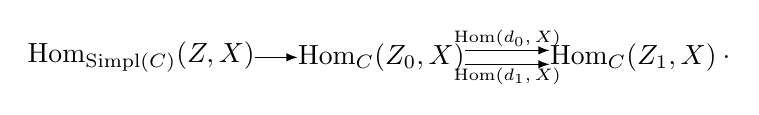
\begin{tikzpicture}[baseline=(b.base),>=latex]
    \node[inner sep=0pt] (a) at (0,0)
      {$\operatorname{Hom}_{\operatorname{Simpl}(C)}(Z,X)$};
    \node[inner sep=0pt] (b) at (3.05,0)
      {$\operatorname{Hom}_{C}(Z_0,X)$};
    \node[inner sep=0pt] (c) at (6.25,0)
      {$\operatorname{Hom}_{C}(Z_1,X)$};
    \draw[->] (a) -- (b);
    \draw[->]
      ([yshift=2.5bp]b.east) --
      node[above,inner sep=1bp,font=\fontsize{5.7}{6.4}\selectfont]
        {$\operatorname{Hom}(d_0,X)$}
      ([yshift=2.5bp]c.west);
    \draw[->]
      ([yshift=-2.5bp]b.east) --
      node[below,inner sep=1bp,font=\fontsize{5.7}{6.4}\selectfont]
        {$\operatorname{Hom}(d_1,X)$}
      ([yshift=-2.5bp]c.west);
    \node[anchor=west,inner sep=0pt,outer sep=0pt] at ([xshift=2bp]c.east) {.};
  \end{tikzpicture}%
}

% END ASSEMBLED SOURCE: tex/common/eq1.tex


% BEGIN ASSEMBLED SOURCE: tex/common/hom1.tex
% Native-TeX homotopy diagrams from LNM 239, physical p.21 / printed p.3.
\newcommand{\IllusieHomotopyTriangle}{%
  \begin{center}
  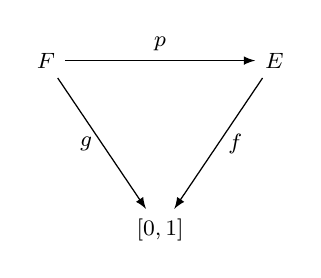
\begin{tikzpicture}[
    >=latex,
    line width=0.45pt,
    every node/.style={font=\rmfamily\fontsize{8}{9}\selectfont}
  ]
    \node (F) at (-1.45,1.0) {$F$};
    \node (E) at (1.45,1.0) {$E$};
    \node (I) at (0,-1.15) {$[0,1]$};
    \draw[->] (F) -- node[above] {$p$} (E);
    \draw[->] (F) -- node[left] {$g$} (I);
    \draw[->] (E) -- node[right] {$f$} (I);
  \end{tikzpicture}
  \end{center}%
}

\newcommand{\IllusieHomotopySquare}{%
  \begin{center}
  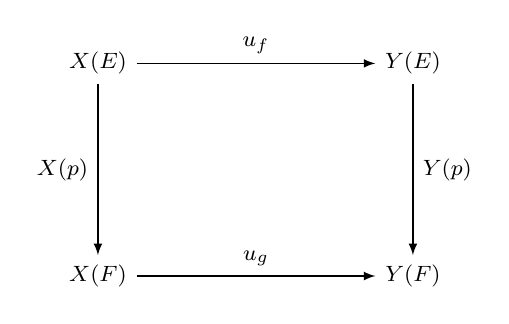
\begin{tikzpicture}[
    >=latex,
    line width=0.45pt,
    every node/.style={font=\rmfamily\fontsize{8}{9}\selectfont}
  ]
    \node (XE) at (-2.0,1.35) {$X(E)$};
    \node (YE) at (2.0,1.35) {$Y(E)$};
    \node (XF) at (-2.0,-1.35) {$X(F)$};
    \node (YF) at (2.0,-1.35) {$Y(F)$};
    \draw[->] (XE) -- node[above] {$u_f$} (YE);
    \draw[->] (XE) -- node[left] {$X(p)$} (XF);
    \draw[->] (YE) -- node[right] {$Y(p)$} (YF);
    \draw[->] (XF) -- node[above] {$u_g$} (YF);
  \end{tikzpicture}
  \end{center}%
}

% END ASSEMBLED SOURCE: tex/common/hom1.tex


% BEGIN ASSEMBLED SOURCE: tex/common/hom2.tex
% Native-TeX pullback square from LNM 239, physical p.58 / printed p.40.
\newcommand{\IllusieHomsPullbackSquare}{%
  \begin{center}
  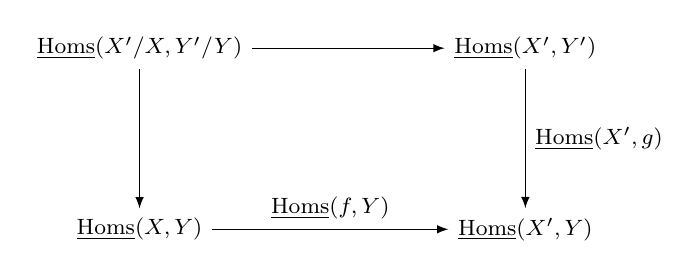
\begin{tikzpicture}[
    >=latex,
    line width=0.42pt,
    every node/.style={font=\rmfamily\fontsize{8.15}{8.8}\selectfont}
  ]
    \node (TL) at (-2.45, 1.15)
      {$\underline{\operatorname{Homs}}(X'/X,Y'/Y)$};
    \node (TR) at ( 2.45, 1.15)
      {$\underline{\operatorname{Homs}}(X',Y')$};
    \node (BL) at (-2.45,-1.15)
      {$\underline{\operatorname{Homs}}(X,Y)$};
    \node (BR) at ( 2.45,-1.15)
      {$\underline{\operatorname{Homs}}(X',Y)$};
    \draw[->] (TL) -- (TR);
    \draw[->] (TL) -- (BL);
    \draw[->] (TR) -- node[right]
      {$\underline{\operatorname{Homs}}(X',g)$} (BR);
    \draw[->] (BL) -- node[above]
      {$\underline{\operatorname{Homs}}(f,Y)$} (BR);
  \end{tikzpicture}
  \end{center}%
}

% END ASSEMBLED SOURCE: tex/common/hom2.tex


% BEGIN ASSEMBLED SOURCE: tex/common/hom3.tex
% Native-TeX mapping-cylinder diagrams from LNM 239, physical p.62 / printed p.44.
\newcommand{\IllusieMappingCylinderTriangle}{%
  \begin{center}
  \begin{tikzpicture}[
    >=latex,
    line width=0.44pt,
    every node/.style={font=\rmfamily\fontsize{8.4}{9}\selectfont}
  ]
    \node (Yp) at (0,1.18) {$Y'$};
    \node (X)  at (-1.65,-0.92) {$X$};
    \node (Y)  at ( 1.65,-0.92) {$Y$};
    \draw[right hook->] (X) -- node[left] {$i$} (Yp);
    \draw[->] (Yp) -- node[right] {$p$} (Y);
    \draw[->] (X) -- node[above] {$f$} (Y);
    \node at (2.35,-0.92) {,};
  \end{tikzpicture}
  \end{center}%
}

\newcommand{\IllusieMappingCylinderPushout}{%
  \begin{center}
  \begin{tikzpicture}[
    >=latex,
    line width=0.44pt,
    every node/.style={font=\rmfamily\fontsize{8.4}{9}\selectfont}
  ]
    \node (DX) at (-2.00, 1.08) {$\Delta(1)\times X$};
    \node (Yp) at ( 2.00, 1.08) {$Y'$};
    \node (X)  at (-2.00,-1.08) {$X$};
    \node (Y)  at ( 2.00,-1.08) {$Y$};
    \draw[->] (DX) -- node[above] {$f'$} (Yp);
    \draw[right hook->] (X) -- node[left] {$d^1$} (DX);
    \draw[right hook->] (Y) -- node[right] {$j$} (Yp);
    \draw[->] (X) -- node[above] {$f$} (Y);
    \node at (2.70,-1.08) {,};
  \end{tikzpicture}
  \end{center}%
}

% END ASSEMBLED SOURCE: tex/common/hom3.tex


% BEGIN ASSEMBLED SOURCE: tex/common/hom4.tex
% Native fraction-calculus diagrams from LNM 239, physical p.63 / printed p.45.
\newcommand{\IllusieFractionProofSource}{%
  \begin{center}
  \begin{tikzpicture}[
    >=latex,line width=0.44pt,
    every node/.style={font=\rmfamily\fontsize{8.4}{9}\selectfont,inner sep=1pt}
  ]
    \node (Xp) at (0,1.15) {$X'$};
    \node (X)  at (0,0) {$X$};
    \node (Y)  at (2.25,0) {$Y$};
    \draw[->] (X) -- node[left] {$s$} (Xp);
    \draw[->] (X) -- node[above] {$u$} (Y);
    \node at (2.85,0) {,};
  \end{tikzpicture}
  \end{center}%
}

\newcommand{\IllusieFractionProofPushout}{%
  \begin{center}
  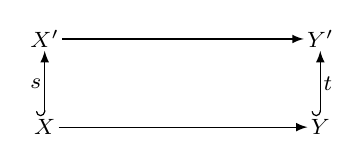
\begin{tikzpicture}[
    >=latex,line width=0.44pt,
    every node/.style={font=\rmfamily\fontsize{8.4}{9}\selectfont,inner sep=1pt}
  ]
    \node (Xp) at (-1.75,1.12) {$X'$};
    \node (Yp) at ( 1.75,1.12) {$Y'$};
    \node (X)  at (-1.75,0) {$X$};
    \node (Y)  at ( 1.75,0) {$Y$};
    \draw[->] (Xp) -- (Yp);
    \draw[right hook->] (X) -- node[left] {$s$} (Xp);
    \draw[right hook->] (Y) -- node[right] {$t$} (Yp);
    \draw[->] (X) -- (Y);
  \end{tikzpicture}
  \end{center}%
}

\newcommand{\IllusieFractionProofParallel}{%
  \begin{center}
  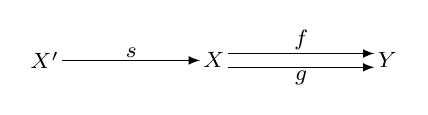
\begin{tikzpicture}[
    >=latex,line width=0.44pt,
    every node/.style={font=\rmfamily\fontsize{8.4}{9}\selectfont,inner sep=1pt}
  ]
    \node (Xp) at (-2.15,0) {$X'$};
    \node (X)  at (0,0) {$X$};
    \node (Y)  at (2.20,0) {$Y$};
    \draw[->] (Xp) -- node[above] {$s$} (X);
    \draw[->] ([yshift=2.5pt]X.east) -- node[above] {$f$} ([yshift=2.5pt]Y.west);
    \draw[->] ([yshift=-2.5pt]X.east) -- node[below] {$g$} ([yshift=-2.5pt]Y.west);
  \end{tikzpicture}
  \end{center}%
}

% END ASSEMBLED SOURCE: tex/common/hom4.tex


% BEGIN ASSEMBLED SOURCE: tex/common/hom5.tex
% Native pushout diagram from LNM 239, physical p.64 / printed p.46.
\newcommand{\IllusieCompositeHomotopyPushouts}{%
  \begin{center}
  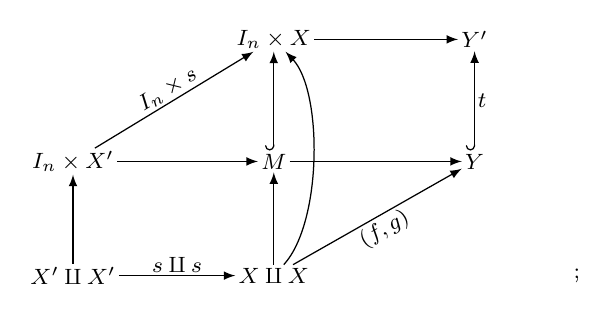
\begin{tikzpicture}[
    >=latex,x=1cm,y=1cm,line width=0.45pt,
    every node/.style={font=\rmfamily\fontsize{8}{9}\selectfont,inner sep=1pt}
  ]
    \node (IX)  at (0,1.55) {$I_n\times X$};
    \node (Yp)  at (2.55,1.55) {$Y'$};
    \node (IXp) at (-2.55,0) {$I_n\times X'$};
    \node (M)   at (0,0) {$M$};
    \node (Y)   at (2.55,0) {$Y$};
    \node (XXp) at (-2.55,-1.45) {$X'\amalg X'$};
    \node (XX)  at (0,-1.45) {$X\amalg X$};

    \draw[->] (IX) -- (Yp);
    \draw[right hook->] (Y) -- node[right] {$t$} (Yp);
    \draw[->] (IXp) -- (M);
    \draw[->] (M) -- (Y);
    \draw[->] (XXp) -- (IXp);
    \draw[->] (XXp) -- node[above] {$s\amalg s$} (XX);
    \draw[->] (XX) -- (M);
    \draw[->] (IXp) -- node[above,sloped] {$I_n\times s$} (IX);
    \draw[right hook->] (M) -- (IX);
    \draw[->] (XX) .. controls (0.62,-0.77) and (0.62,0.90) .. (IX);
    \draw[->] (XX) -- node[below,sloped] {$(f,g)$} (Y);
    \node at (3.85,-1.45) {$;$};
  \end{tikzpicture}
  \end{center}%
}

% END ASSEMBLED SOURCE: tex/common/hom5.tex


% BEGIN ASSEMBLED SOURCE: tex/common/hom6.tex
% Native lifting diagrams from LNM 239, physical p.65 / printed p.47.
\newcommand{\IllusieLocalLiftingSquare}{%
  \begin{center}
  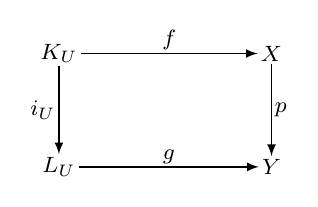
\begin{tikzpicture}[
    >=latex,x=1cm,y=1cm,line width=0.45pt,
    every node/.style={font=\rmfamily\fontsize{8}{9}\selectfont,inner sep=1pt}
  ]
    \node (KU) at (-1.35,0.72) {$K_U$};
    \node (X)  at (1.35,0.72) {$X$};
    \node (LU) at (-1.35,-0.72) {$L_U$};
    \node (Y)  at (1.35,-0.72) {$Y$};
    \draw[->] (KU) -- node[above] {$f$} (X);
    \draw[->] (KU) -- node[left] {$i_U$} (LU);
    \draw[->] (X) -- node[right] {$p$} (Y);
    \draw[->] (LU) -- node[above] {$g$} (Y);
  \end{tikzpicture}
  \end{center}%
}

\newcommand{\IllusieLocalLiftDiagram}{%
  \begin{center}
  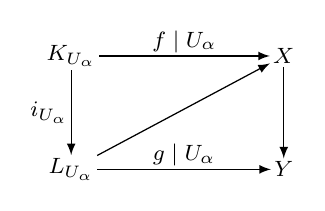
\begin{tikzpicture}[
    >=latex,x=1cm,y=1cm,line width=0.45pt,
    every node/.style={font=\rmfamily\fontsize{8}{9}\selectfont,inner sep=1pt}
  ]
    \node (KU) at (-1.35,0.72) {$K_{U_\alpha}$};
    \node (X)  at (1.35,0.72) {$X$};
    \node (LU) at (-1.35,-0.72) {$L_{U_\alpha}$};
    \node (Y)  at (1.35,-0.72) {$Y$};
    \draw[->] (KU) -- node[above] {$f\mid U_\alpha$} (X);
    \draw[->] (KU) -- node[left] {$i_{U_\alpha}$} (LU);
    \draw[->] (X) -- (Y);
    \draw[->] (LU) -- node[above] {$g\mid U_\alpha$} (Y);
    \draw[->] (LU) -- (X);
  \end{tikzpicture}
  \end{center}%
}

% END ASSEMBLED SOURCE: tex/common/hom6.tex


% BEGIN ASSEMBLED SOURCE: tex/common/tri1.tex
% Native-TeX transitivity triangle from LNM 239, physical p.12 / Roman X.
\newcommand{\IllusieTransitivityTriangle}{%
  \begin{center}
  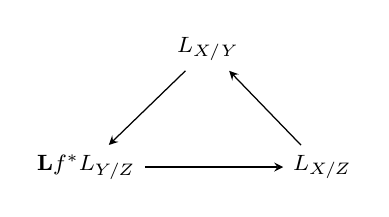
\begin{tikzpicture}[
    >=stealth,
    line width=0.45pt,
    every node/.style={font=\rmfamily\fontsize{8.15}{9}\selectfont}
  ]
    \node (xy) at (0,1.05) {$L_{X/Y}$};
    \node (fyz) at (-1.55,-0.45) {$\mathbf L f^{*}L_{Y/Z}$};
    \node (xz) at (1.45,-0.45) {$L_{X/Z}$};
    \draw[->] (xy) -- (fyz);
    \draw[->] (fyz) -- (xz);
    \draw[->] (xz) -- (xy);
  \end{tikzpicture}
  \end{center}%
}

% END ASSEMBLED SOURCE: tex/common/tri1.tex


% BEGIN ASSEMBLED SOURCE: tex/common/guide1.tex
% Native chapter-dependency guide from LNM 239 physical p.17 / Roman XV.
\newcommand{\IllusieChapterGuide}{%
  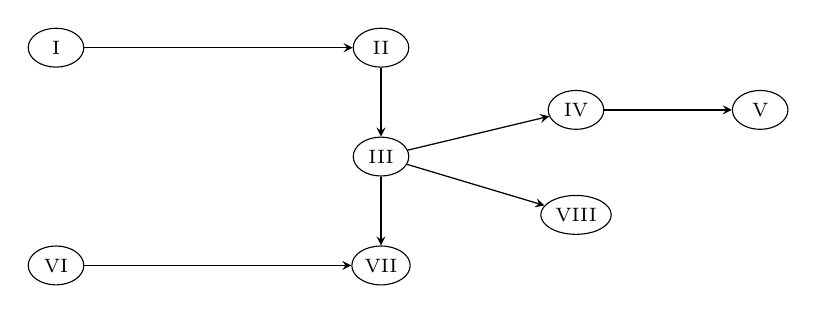
\begin{tikzpicture}[
    x=39bp,y=28bp,>=stealth,
    guide node/.style={draw,ellipse,minimum width=20bp,minimum height=14bp,
      inner sep=1.5bp,font=\fontsize{7}{7}\selectfont},
    guide arrow/.style={->,line width=0.45pt}
  ]
    \node[guide node] (I) at (0,2.8) {I};
    \node[guide node] (II) at (3,2.8) {II};
    \node[guide node] (III) at (3,1.4) {III};
    \node[guide node] (IV) at (4.8,2.0) {IV};
    \node[guide node] (V) at (6.5,2.0) {V};
    \node[guide node] (VIII) at (4.8,0.65) {VIII};
    \node[guide node] (VII) at (3,0) {VII};
    \node[guide node] (VI) at (0,0) {VI};
    \draw[guide arrow] (I) -- (II);
    \draw[guide arrow] (II) -- (III);
    \draw[guide arrow] (III) -- (IV);
    \draw[guide arrow] (IV) -- (V);
    \draw[guide arrow] (III) -- (VIII);
    \draw[guide arrow] (III) -- (VII);
    \draw[guide arrow] (VI) -- (VII);
  \end{tikzpicture}%
}

% END ASSEMBLED SOURCE: tex/common/guide1.tex


% BEGIN ASSEMBLED SOURCE: tex/common/assoc1.tex
% Native-TeX associativity/coassociativity squares from LNM 239,
% physical p.26 / printed p.8, formula (1.2.2.3).
\newcommand{\IllusieAssociativitySquares}{%
  \begin{center}
  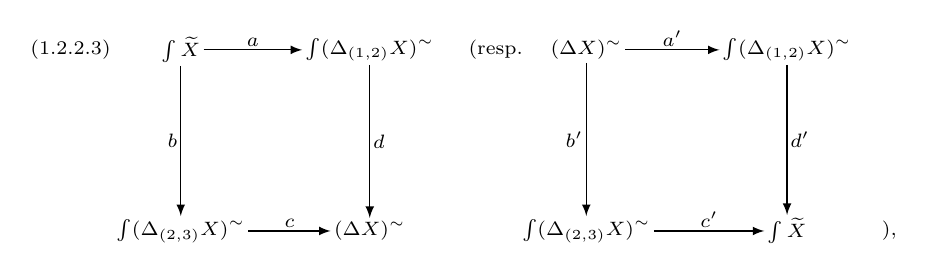
\begin{tikzpicture}[
    >=latex,
    x=1cm,
    y=1cm,
    line width=0.45pt,
    every node/.style={font=\rmfamily\fontsize{7.2}{8}\selectfont,inner sep=1pt}
  ]
    \node at (-6.35,1.15) {(1.2.2.3)};

    \node (LTL) at (-4.95,1.15) {$\int\widetilde X$};
    \node (LTR) at (-2.55,1.15) {$\int(\Delta_{(1,2)}X)^{\sim}$};
    \node (LBL) at (-4.95,-1.15) {$\int(\Delta_{(2,3)}X)^{\sim}$};
    \node (LBR) at (-2.55,-1.15) {$(\Delta X)^{\sim}$};
    \draw[->] (LTL) -- node[above] {$a$} (LTR);
    \draw[->] (LTL) -- node[left] {$b$} (LBL);
    \draw[->] (LBL) -- node[above] {$c$} (LBR);
    \draw[->] (LTR) -- node[right] {$d$} (LBR);

    \node at (-0.95,1.15) {(resp.};
    \node (RTL) at (0.20,1.15) {$(\Delta X)^{\sim}$};
    \node (RTR) at (2.75,1.15) {$\int(\Delta_{(1,2)}X)^{\sim}$};
    \node (RBL) at (0.20,-1.15) {$\int(\Delta_{(2,3)}X)^{\sim}$};
    \node (RBR) at (2.75,-1.15) {$\int\widetilde X$};
    \draw[->] (RTL) -- node[above] {$a'$} (RTR);
    \draw[->] (RTL) -- node[left] {$b'$} (RBL);
    \draw[->] (RBL) -- node[above] {$c'$} (RBR);
    \draw[->] (RTR) -- node[right] {$d'$} (RBR);
    \node at (4.05,-1.15) {),};
  \end{tikzpicture}
  \end{center}%
}

% END ASSEMBLED SOURCE: tex/common/assoc1.tex


% BEGIN ASSEMBLED SOURCE: tex/common/dold1.tex
% Native-TeX factorization square from LNM 239,
% physical p.27 / printed p.9, section 1.3.1.
\newcommand{\IllusieDoldPuppeSquare}{%
  \begin{center}
  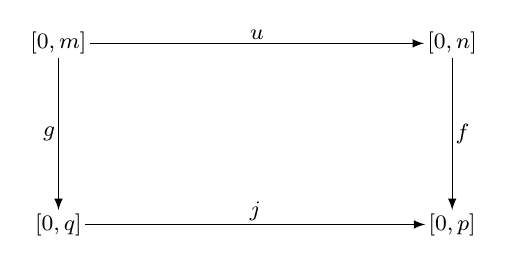
\begin{tikzpicture}[
    >=latex,
    x=1cm,
    y=1cm,
    line width=0.45pt,
    every node/.style={font=\rmfamily\fontsize{8}{9}\selectfont,inner sep=1pt}
  ]
    \node (TL) at (-2.5,1.15) {$[0,m]$};
    \node (TR) at (2.5,1.15) {$[0,n]$};
    \node (BL) at (-2.5,-1.15) {$[0,q]$};
    \node (BR) at (2.5,-1.15) {$[0,p]$};
    \draw[->] (TL) -- node[above] {$u$} (TR);
    \draw[->] (TL) -- node[left] {$g$} (BL);
    \draw[->] (TR) -- node[right] {$f$} (BR);
    \draw[->] (BL) -- node[above] {$j$} (BR);
  \end{tikzpicture}
  \end{center}%
}

% END ASSEMBLED SOURCE: tex/common/dold1.tex


% BEGIN ASSEMBLED SOURCE: tex/common/dold2.tex
% Native normal/degenerate restriction diagram from LNM 239,
% physical p.29 / printed p.11, section 1.3.5.
\newcommand{\IllusieNormalDegenerateDiagram}{%
  \begin{center}
  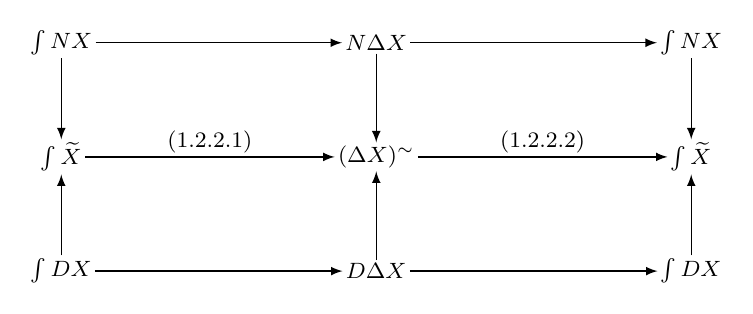
\begin{tikzpicture}[
    >=latex,
    x=1cm,
    y=1cm,
    line width=0.45pt,
    every node/.style={font=\rmfamily\fontsize{8}{9}\selectfont,inner sep=1pt}
  ]
    \node (TL) at (-4.0,1.45) {$\int NX$};
    \node (TC) at (0,1.45) {$N\Delta X$};
    \node (TR) at (4.0,1.45) {$\int NX$};
    \node (ML) at (-4.0,0) {$\int\widetilde X$};
    \node (MC) at (0,0) {$(\Delta X)^{\sim}$};
    \node (MR) at (4.0,0) {$\int\widetilde X$};
    \node (BL) at (-4.0,-1.45) {$\int DX$};
    \node (BC) at (0,-1.45) {$D\Delta X$};
    \node (BR) at (4.0,-1.45) {$\int DX$};

    \draw[->] (TL) -- (TC);
    \draw[->] (TC) -- (TR);
    \draw[->] (ML) -- node[above] {(1.2.2.1)} (MC);
    \draw[->] (MC) -- node[above] {(1.2.2.2)} (MR);
    \draw[->] (BL) -- (BC);
    \draw[->] (BC) -- (BR);
    \draw[->] (TL) -- (ML);
    \draw[->] (TC) -- (MC);
    \draw[->] (TR) -- (MR);
    \draw[->] (BL) -- (ML);
    \draw[->] (BC) -- (MC);
    \draw[->] (BR) -- (MR);
  \end{tikzpicture}
  \end{center}%
}

% END ASSEMBLED SOURCE: tex/common/dold2.tex


% BEGIN ASSEMBLED SOURCE: tex/common/fractions1.tex
% Native right/left calculus-of-fractions diagrams from LNM 239,
% physical p.30 / printed p.12, section 1.4.2.
\newcommand{\IllusieRightFractionFrThreeSource}{%
  \begin{center}
  \begin{tikzpicture}[
    >=latex,x=1cm,y=1cm,line width=0.45pt,
    every node/.style={font=\rmfamily\fontsize{8}{9}\selectfont,inner sep=1pt}
  ]
    \node (X) at (-1.7,0) {$X$};
    \node (Y) at (1.7,0) {$Y$};
    \node (Yp) at (1.7,1.35) {$Y'$};
    \draw[->] (X) -- node[above] {$u$} (Y);
    \draw[->] (Yp) -- node[right] {$t$} (Y);
  \end{tikzpicture}
  \end{center}%
}

\newcommand{\IllusieRightFractionFrThreeCompletion}{%
  \begin{center}
  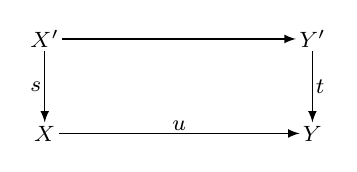
\begin{tikzpicture}[
    >=latex,x=1cm,y=1cm,line width=0.45pt,
    every node/.style={font=\rmfamily\fontsize{8}{9}\selectfont,inner sep=1pt}
  ]
    \node (Xp) at (-1.7,1.2) {$X'$};
    \node (Yp) at (1.7,1.2) {$Y'$};
    \node (X) at (-1.7,0) {$X$};
    \node (Y) at (1.7,0) {$Y$};
    \draw[->] (Xp) -- (Yp);
    \draw[->] (Xp) -- node[left] {$s$} (X);
    \draw[->] (Yp) -- node[right] {$t$} (Y);
    \draw[->] (X) -- node[above] {$u$} (Y);
  \end{tikzpicture}
  \end{center}%
}

\newcommand{\IllusieRightFractionFrFourSource}{%
  \begin{center}
  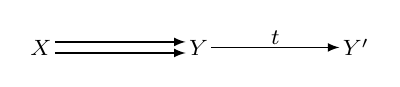
\begin{tikzpicture}[
    >=latex,x=1cm,y=1cm,line width=0.45pt,
    every node/.style={font=\rmfamily\fontsize{8}{9}\selectfont,inner sep=1pt}
  ]
    \node (X) at (-2.0,0) {$X$};
    \node (Y) at (0,0) {$Y$};
    \node (Yp) at (2.0,0) {$Y'$};
    \draw[->] ([yshift=2pt]X.east) -- ([yshift=2pt]Y.west);
    \draw[->] ([yshift=-2pt]X.east) -- ([yshift=-2pt]Y.west);
    \draw[->] (Y) -- node[above] {$t$} (Yp);
  \end{tikzpicture}
  \end{center}%
}

\newcommand{\IllusieRightFractionFrFourCompletion}{%
  \begin{center}
  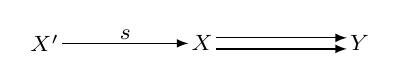
\begin{tikzpicture}[
    >=latex,x=1cm,y=1cm,line width=0.45pt,
    every node/.style={font=\rmfamily\fontsize{8}{9}\selectfont,inner sep=1pt}
  ]
    \node (Xp) at (-2.0,0) {$X'$};
    \node (X) at (0,0) {$X$};
    \node (Y) at (2.0,0) {$Y$};
    \draw[->] (Xp) -- node[above] {$s$} (X);
    \draw[->] ([yshift=2pt]X.east) -- ([yshift=2pt]Y.west);
    \draw[->] ([yshift=-2pt]X.east) -- ([yshift=-2pt]Y.west);
  \end{tikzpicture}
  \end{center}%
}

\newcommand{\IllusieLeftFractionFrThreeSource}{%
  \begin{center}
  \begin{tikzpicture}[
    >=latex,x=1cm,y=1cm,line width=0.45pt,
    every node/.style={font=\rmfamily\fontsize{8}{9}\selectfont,inner sep=1pt}
  ]
    \node (X) at (-1.5,0.8) {$X$};
    \node (Y) at (1.5,0.8) {$Y$};
    \node (Xp) at (-1.5,-0.65) {$X'$};
    \draw[->] (X) -- node[above] {$u$} (Y);
    \draw[->] (X) -- node[left] {$s$} (Xp);
  \end{tikzpicture}
  \end{center}%
}

\newcommand{\IllusieLeftFractionFrThreeCompletion}{%
  \begin{center}
  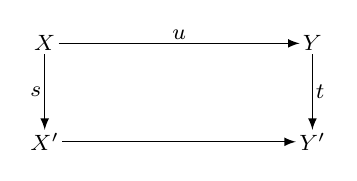
\begin{tikzpicture}[
    >=latex,x=1cm,y=1cm,line width=0.45pt,
    every node/.style={font=\rmfamily\fontsize{8}{9}\selectfont,inner sep=1pt}
  ]
    \node (X) at (-1.7,1.25) {$X$};
    \node (Y) at (1.7,1.25) {$Y$};
    \node (Xp) at (-1.7,0) {$X'$};
    \node (Yp) at (1.7,0) {$Y'$};
    \draw[->] (X) -- node[above] {$u$} (Y);
    \draw[->] (X) -- node[left] {$s$} (Xp);
    \draw[->] (Y) -- node[right] {$t$} (Yp);
    \draw[->] (Xp) -- (Yp);
  \end{tikzpicture}
  \end{center}%
}

\newcommand{\IllusieLeftFractionFrFourSource}{%
  \begin{center}
  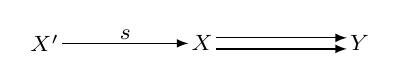
\begin{tikzpicture}[
    >=latex,x=1cm,y=1cm,line width=0.45pt,
    every node/.style={font=\rmfamily\fontsize{8}{9}\selectfont,inner sep=1pt}
  ]
    \node (Xp) at (-2.0,0) {$X'$};
    \node (X) at (0,0) {$X$};
    \node (Y) at (2.0,0) {$Y$};
    \draw[->] (Xp) -- node[above] {$s$} (X);
    \draw[->] ([yshift=2pt]X.east) -- ([yshift=2pt]Y.west);
    \draw[->] ([yshift=-2pt]X.east) -- ([yshift=-2pt]Y.west);
  \end{tikzpicture}
  \end{center}%
}

\newcommand{\IllusieLeftFractionFrFourCompletion}{%
  \begin{center}
  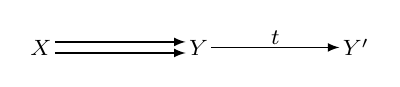
\begin{tikzpicture}[
    >=latex,x=1cm,y=1cm,line width=0.45pt,
    every node/.style={font=\rmfamily\fontsize{8}{9}\selectfont,inner sep=1pt}
  ]
    \node (X) at (-2.0,0) {$X$};
    \node (Y) at (0,0) {$Y$};
    \node (Yp) at (2.0,0) {$Y'$};
    \draw[->] ([yshift=2pt]X.east) -- ([yshift=2pt]Y.west);
    \draw[->] ([yshift=-2pt]X.east) -- ([yshift=-2pt]Y.west);
    \draw[->] (Y) -- node[above] {$t$} (Yp);
  \end{tikzpicture}
  \end{center}%
}

% END ASSEMBLED SOURCE: tex/common/fractions1.tex


% BEGIN ASSEMBLED SOURCE: tex/common/derived1.tex
% Native 2-cell diagram from LNM 239, physical p.32 / printed p.14,
% section 1.4.4. The 2-cell v has target F, as does u_F.
\newcommand{\IllusieLeftDerivedUniversalTriangle}{%
  \begin{center}
  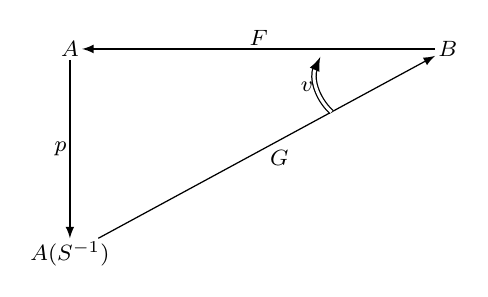
\begin{tikzpicture}[
    >=latex,x=1cm,y=1cm,line width=0.45pt,
    every node/.style={font=\rmfamily\fontsize{8}{9}\selectfont,inner sep=1pt}
  ]
    \node (A) at (-2.4,1.5) {$A$};
    \node (AS) at (-2.4,-1.1) {$A(S^{-1})$};
    \node (B) at (2.4,1.5) {$B$};
    \draw[->] (B) -- node[above] {$F$} (A);
    \draw[->] (A) -- node[left] {$p$} (AS);
    \draw[->] (AS) -- node[below right] {$G$} (B);
    \draw[double distance=1.1pt,->]
      (0.92,0.70) to[bend left=35] node[left] {$v$} (0.78,1.40);
  \end{tikzpicture}
  \end{center}%
}

% END ASSEMBLED SOURCE: tex/common/derived1.tex


% BEGIN ASSEMBLED SOURCE: tex/common/derived2.tex
% Native comparison grid from LNM 239, physical p.33 / printed p.15,
% section 1.4.5. Horizontal arrows are N and K; vertical arrows localize.
\newcommand{\IllusieDerivedComparisonGrid}{%
  \begin{center}
  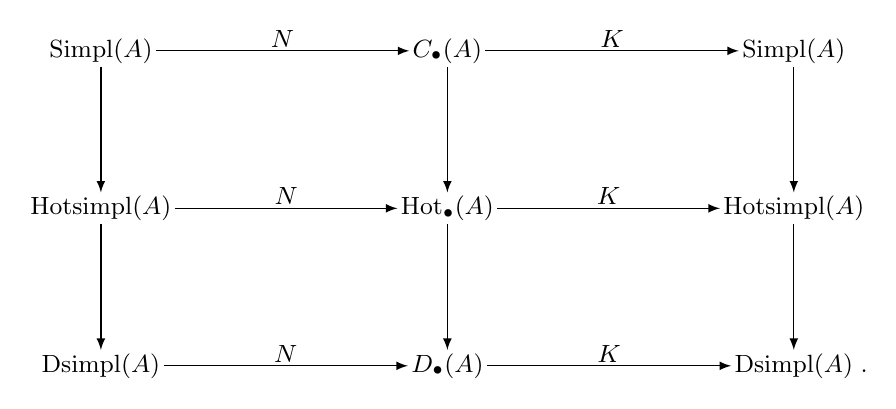
\begin{tikzpicture}[
    >=latex,x=1cm,y=1cm,line width=0.45pt,
    every node/.style={font=\rmfamily\fontsize{9}{10}\selectfont,inner sep=1pt}
  ]
    \node (s0) at (-4.4,2) {$\operatorname{Simpl}(A)$};
    \node (c0) at (0,2) {$C_{\bullet}(A)$};
    \node (s1) at (4.4,2) {$\operatorname{Simpl}(A)$};
    \node (hs0) at (-4.4,0) {$\operatorname{Hotsimpl}(A)$};
    \node (hc0) at (0,0) {$\operatorname{Hot}_{\bullet}(A)$};
    \node (hs1) at (4.4,0) {$\operatorname{Hotsimpl}(A)$};
    \node (ds0) at (-4.4,-2) {$\operatorname{Dsimpl}(A)$};
    \node (dc0) at (0,-2) {$D_{\bullet}(A)$};
    \node (ds1) at (4.4,-2) {$\operatorname{Dsimpl}(A)$};

    \draw[->] (s0) -- node[above] {$N$} (c0);
    \draw[->] (c0) -- node[above] {$K$} (s1);
    \draw[->] (hs0) -- node[above] {$N$} (hc0);
    \draw[->] (hc0) -- node[above] {$K$} (hs1);
    \draw[->] (ds0) -- node[above] {$N$} (dc0);
    \draw[->] (dc0) -- node[above] {$K$} (ds1);

    \draw[->] (s0) -- (hs0);
    \draw[->] (c0) -- (hc0);
    \draw[->] (s1) -- (hs1);
    \draw[->] (hs0) -- (ds0);
    \draw[->] (hc0) -- (dc0);
    \draw[->] (hs1) -- (ds1);
    \node[anchor=base west,inner sep=0pt,outer sep=0pt] at ([xshift=1.5pt]ds1.base east) {.};
  \end{tikzpicture}
  \end{center}%
}

% END ASSEMBLED SOURCE: tex/common/derived2.tex


% BEGIN ASSEMBLED SOURCE: tex/common/local2.tex
% Native-TeX diagrams for Lemma 2.2.6, LNM 239 physical p.47 / printed p.29.
\newcommand{\IllusieLocalObjectSquare}{%
  \begin{center}
  \begin{tikzpicture}[
    >=latex,
    line width=0.45pt,
    every node/.style={font=\rmfamily\fontsize{9.3}{10.4}\selectfont}
  ]
    \node (Ei) at (-2.0,1.55) {$E_i$};
    \node (Fi) at ( 2.0,1.55) {$F_i$};
    \node (EU) at (-2.0,-1.55) {$E(U)$};
    \node (FU) at ( 2.0,-1.55) {$F(U)$};
    \draw[->] (Ei) -- node[above] {$u_i$} (Fi);
    \draw[->] (Ei) -- (EU);
    \draw[->] (Fi) -- (FU);
    \draw[->] (EU) -- node[above] {$u(U)$} (FU);
    \node at (2.55,-1.55) {,};
  \end{tikzpicture}
  \end{center}%
}

\newcommand{\IllusieLocalRestrictionSquare}{%
  \begin{center}
  \begin{tikzpicture}[
    >=latex,
    line width=0.45pt,
    every node/.style={font=\rmfamily\fontsize{9.3}{10.4}\selectfont}
  ]
    \node (Ei) at (-2.0,1.55) {$E_i$};
    \node (Fi) at ( 2.0,1.55) {$F_i$};
    \node (EU) at (-2.0,-1.55) {$E\vert U$};
    \node (FU) at ( 2.0,-1.55) {$F\vert U$};
    \draw[->] (Ei) -- node[above] {$u_i$} (Fi);
    \draw[->] (Ei) -- (EU);
    \draw[->] (Fi) -- (FU);
    \draw (EU) -- node[above] {$u\vert U$} (FU);
    \node at (2.55,-1.55) {,};
  \end{tikzpicture}
  \end{center}%
}

\newcommand{\IllusieLocalMorphismTriangle}{%
  \begin{center}
  \begin{tikzpicture}[
    >=latex,
    line width=0.45pt,
    every node/.style={font=\rmfamily\fontsize{9.3}{10.4}\selectfont}
  ]
    \node (ui) at (-1.75,1.25) {$u_i$};
    \node (uj) at ( 1.75,1.25) {$u_j$};
    \node (u)  at (0,-1.25) {$u(U)$};
    \draw[->] (ui) -- node[above] {$f$} (uj);
    \draw[->] (ui) -- node[left] {$i$} (u);
    \draw[->] (uj) -- node[right] {$j$} (u);
    \node at (2.25,-1.25) {.};
  \end{tikzpicture}
  \end{center}%
}

% END ASSEMBLED SOURCE: tex/common/local2.tex


% BEGIN ASSEMBLED SOURCE: tex/common/local3.tex
% Native-TeX diagram for Lemma 2.2.6, LNM 239 physical p.48 / printed p.30.
\newcommand{\IllusieFinitePresentationCube}{%
  \begin{center}
  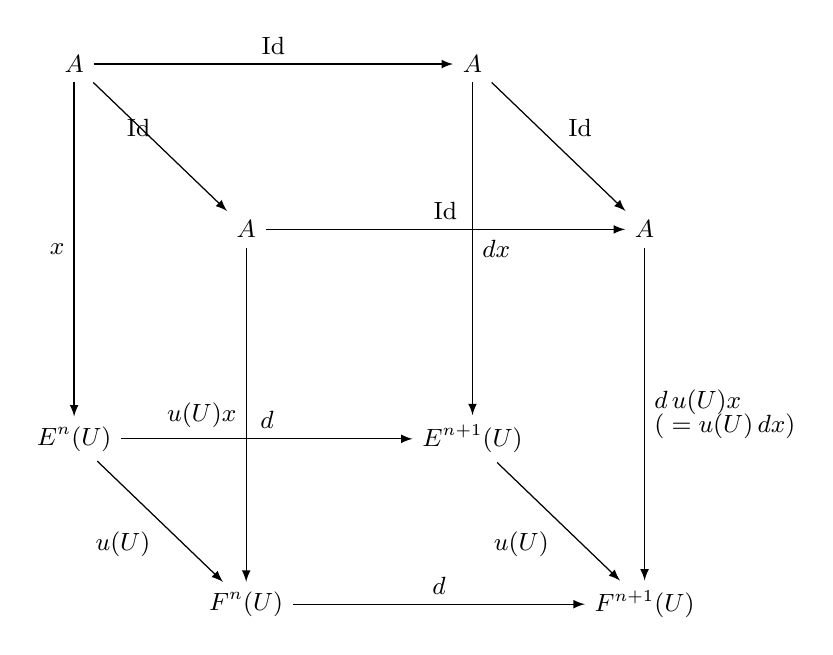
\begin{tikzpicture}[
    x=1.15cm,
    y=1.40cm,
    >=latex,
    line width=0.45pt,
    every node/.style={font=\rmfamily\fontsize{8.8}{9.8}\selectfont}
  ]
    \node (A0) at (-3.2, 2.6) {$A$};
    \node (A1) at ( 1.2, 2.6) {$A$};
    \node (B0) at (-1.3, 1.1) {$A$};
    \node (B1) at ( 3.1, 1.1) {$A$};
    \node (E0) at (-3.2,-0.8) {$E^n(U)$};
    \node (E1) at ( 1.2,-0.8) {$E^{n+1}(U)$};
    \node (F0) at (-1.3,-2.3) {$F^n(U)$};
    \node (F1) at ( 3.1,-2.3) {$F^{n+1}(U)$};
    \draw[->] (A0) -- node[above] {$\operatorname{Id}$} (A1);
    \draw[->] (A0) -- node[above left] {$\operatorname{Id}$} (B0);
    \draw[->] (A1) -- node[above right] {$\operatorname{Id}$} (B1);
    \draw[->] (B0) -- node[above] {$\operatorname{Id}$} (B1);
    \draw[->] (A0) -- node[left] {$x$} (E0);
    \draw[->] (A1) -- node[right] {$dx$} (E1);
    \draw[->] (B0) -- node[left] {$u(U)x$} (F0);
    \draw[->] (B1) -- node[right,align=left] {$d\,u(U)x$\\[-1pt]$({}=u(U)\,dx)$} (F1);
    \draw[->] (E0) -- node[above] {$d$} (E1);
    \draw[->] (F0) -- node[above] {$d$} (F1);
    \draw[->] (E0) -- node[below left] {$u(U)$} (F0);
    \draw[->] (E1) -- node[below left] {$u(U)$} (F1);
  \end{tikzpicture}
  \end{center}%
}

% END ASSEMBLED SOURCE: tex/common/local3.tex


% BEGIN ASSEMBLED SOURCE: tex/common/local4.tex
% Native-TeX diagram for Lemma 2.2.7, LNM 239 physical p.49 / printed p.31.
\newcommand{\IllusieExtensionLemmaTriangle}{%
  \begin{center}
  \begin{tikzpicture}[
    >=latex,
    line width=0.42pt,
    every node/.style={font=\rmfamily\fontsize{8.15}{9.2}\selectfont}
  ]
    \node (z0) at (-4.10, 1.15) {$0$};
    \node (up) at (-2.55, 1.15) {$u'$};
    \node (upp) at (-0.35, 1.15) {$u''_{\alpha}$};
    \node (va) at ( 1.95, 1.15) {$v_{\alpha}$};
    \node (z1) at ( 3.75, 1.15) {$0$};
    \node (ua) at (-1.20,-1.55) {$u(U_{\alpha})$};
    \draw[->] (z0) -- (up);
    \draw[->] (up) -- (upp);
    \draw[->] (upp) -- (va);
    \draw[->] (va) -- (z1);
    \draw[->] (up) -- node[below left] {$f\vert U_{\alpha}$} (ua);
    \draw[->] (upp) -- (ua);
    \node at (2.95,-1.10) {,};
  \end{tikzpicture}
  \end{center}%
}

% END ASSEMBLED SOURCE: tex/common/local4.tex


% BEGIN ASSEMBLED SOURCE: tex/common/local5.tex
% Native-TeX diagrams for Lemma 2.2.7, LNM 239 physical p.50 / printed p.32.
\newcommand{\IllusieRTSquare}{%
  \begin{center}
  \begin{tikzpicture}[>=latex,line width=0.42pt,every node/.style={font=\rmfamily\fontsize{8.15}{9.2}\selectfont}]
    \node (M)  at (-2.80, 1.15) {$M$};
    \node (ZE) at ( 1.75, 1.15) {$Z^{n+1}(E')$};
    \node (Fn) at (-2.80,-1.15) {$F'^{n}$};
    \node (ZF) at ( 1.75,-1.15) {$Z^{n+1}(F')$};
    \draw[->] (M) -- node[above] {$r$} (ZE);
    \draw[->] (M) -- node[left] {$t$} (Fn);
    \draw[->] (ZE) -- node[right] {$u'$} (ZF);
    \draw[->] (Fn) -- (ZF);
    \node at (3.35,-1.15) {.};
  \end{tikzpicture}
  \end{center}%
}

\newcommand{\IllusieCohomologyRectangle}{%
  \begin{center}
  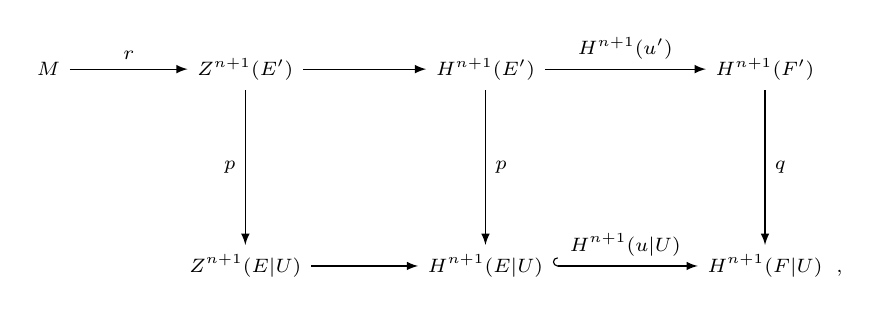
\begin{tikzpicture}[>=latex,line width=0.42pt,every node/.style={font=\rmfamily\fontsize{7.4}{8.5}\selectfont}]
    \node (M)   at (-5.65, 1.20) {$M$};
    \node (ZE)  at (-3.15, 1.20) {$Z^{n+1}(E')$};
    \node (HE)  at (-0.10, 1.20) {$H^{n+1}(E')$};
    \node (HF)  at ( 3.45, 1.20) {$H^{n+1}(F')$};
    \node (ZEU) at (-3.15,-1.30) {$Z^{n+1}(E\vert U)$};
    \node (HEU) at (-0.10,-1.30) {$H^{n+1}(E\vert U)$};
    \node (HFU) at ( 3.45,-1.30) {$H^{n+1}(F\vert U)$};
    \draw[->] (M) -- node[above] {$r$} (ZE);
    \draw[->] (ZE) -- (HE);
    \draw[->] (HE) -- node[above] {$H^{n+1}(u')$} (HF);
    \draw[->] (ZE) -- node[left] {$p$} (ZEU);
    \draw[->] (HE) -- node[right] {$p$} (HEU);
    \draw[->] (HF) -- node[right] {$q$} (HFU);
    \draw[->] (ZEU) -- (HEU);
    \draw[right hook->] (HEU) -- node[above] {$H^{n+1}(u\vert U)$} (HFU);
    \node[anchor=base west,inner sep=0pt,outer sep=0pt] at ([xshift=1.5pt]HFU.base east) {,};
  \end{tikzpicture}
  \end{center}%
}

\newcommand{\IllusieLocalizedSSquare}{%
  \begin{center}
  \begin{tikzpicture}[>=latex,line width=0.42pt,every node/.style={font=\rmfamily\fontsize{8.15}{9.2}\selectfont}]
    \node (M)   at (-2.80, 1.15) {$M$};
    \node (ZE)  at ( 1.75, 1.15) {$Z^{n+1}(E')$};
    \node (EnU) at (-2.80,-1.15) {$E^{n}\vert U$};
    \node (ZEU) at ( 1.75,-1.15) {$Z^{n+1}(E\vert U)$};
    \draw[->] (M) -- node[above] {$r$} (ZE);
    \draw[->] (M) -- node[left] {$s$} (EnU);
    \draw[->] (ZE) -- (ZEU);
    \draw[->] (EnU) -- (ZEU);
    \node[anchor=base west,inner sep=0pt,outer sep=0pt] at ([xshift=1.5pt]ZEU.base east) {.};
  \end{tikzpicture}
  \end{center}%
}

\newcommand{\IllusieTSQUquare}{%
  \begin{center}
  \begin{tikzpicture}[>=latex,line width=0.42pt,every node/.style={font=\rmfamily\fontsize{8.15}{9.2}\selectfont}]
    \node (M)   at (-2.80, 1.15) {$M$};
    \node (Fpn) at ( 1.75, 1.15) {$F'^{n}$};
    \node (EnU) at (-2.80,-1.15) {$E^{n}\vert U$};
    \node (FnU) at ( 1.75,-1.15) {$F^{n}\vert U$};
    \draw[->] (M) -- node[above] {$t$} (Fpn);
    \draw[->] (M) -- node[left] {$s$} (EnU);
    \draw[->] (Fpn) -- node[right] {$q$} (FnU);
    \draw[->] (EnU) -- node[above] {$u$} (FnU);
  \end{tikzpicture}
  \end{center}%
}

% END ASSEMBLED SOURCE: tex/common/local5.tex


% BEGIN ASSEMBLED SOURCE: tex/common/local6.tex
% Native-TeX diagrams for Lemma 2.2.7, LNM 239 physical p.51 / printed p.33.
\newcommand{\IllusieUDoublePrimeComplexMap}{%
  \begin{center}
  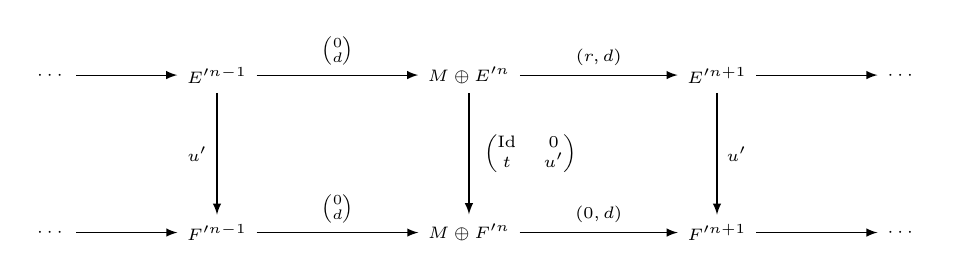
\begin{tikzpicture}[>=latex,line width=0.4pt,every node/.style={font=\rmfamily\fontsize{5.7}{6.2}\selectfont}]
    \node (ET0) at (-5.65, 1.00) {$\cdots$};
    \node (ET1) at (-3.55, 1.00) {$E'^{n-1}$};
    \node (ET2) at (-0.35, 1.00) {$M\oplus E'^n$};
    \node (ET3) at ( 2.80, 1.00) {$E'^{n+1}$};
    \node (ET4) at ( 5.15, 1.00) {$\cdots$};
    \node (FB0) at (-5.65,-1.00) {$\cdots$};
    \node (FB1) at (-3.55,-1.00) {$F'^{n-1}$};
    \node (FB2) at (-0.35,-1.00) {$M\oplus F'^n$};
    \node (FB3) at ( 2.80,-1.00) {$F'^{n+1}$};
    \node (FB4) at ( 5.15,-1.00) {$\cdots$};
    \draw[->] (ET0) -- (ET1); \draw[->] (ET1) -- node[above] {$\binom{0}{d}$} (ET2);
    \draw[->] (ET2) -- node[above] {$(r,d)$} (ET3); \draw[->] (ET3) -- (ET4);
    \draw[->] (FB0) -- (FB1); \draw[->] (FB1) -- node[above] {$\binom{0}{d}$} (FB2);
    \draw[->] (FB2) -- node[above] {$(0,d)$} (FB3); \draw[->] (FB3) -- (FB4);
    \draw[->] (ET1) -- node[left] {$u'$} (FB1);
    \draw[->] (ET2) -- node[right,xshift=2pt] {$\begin{pmatrix}\mathrm{Id}&0\\ t&u'\end{pmatrix}$} (FB2);
    \draw[->] (ET3) -- node[right] {$u'$} (FB3);
  \end{tikzpicture}
  \end{center}%
}

\newcommand{\IllusiePPrimeComplexMap}{%
  \begin{center}
  \begin{tikzpicture}[>=latex,line width=0.4pt,every node/.style={font=\rmfamily\fontsize{5.7}{6.2}\selectfont}]
    \node (ET0) at (-5.65, 1.00) {$\cdots$};
    \node (ET1) at (-3.55, 1.00) {$E'^{n-1}$};
    \node (ET2) at (-0.35, 1.00) {$M\oplus E'^n$};
    \node (ET3) at ( 2.80, 1.00) {$E'^{n+1}$};
    \node (ET4) at ( 5.15, 1.00) {$\cdots$};
    \node at (5.75,1.00) {,};
    \node (EB0) at (-5.65,-1.00) {$\cdots$};
    \node (EB1) at (-3.55,-1.00) {$E^{n-1}\vert U$};
    \node (EB2) at (-0.35,-1.00) {$E^n\vert U$};
    \node (EB3) at ( 2.80,-1.00) {$E^{n+1}\vert U$};
    \node (EB4) at ( 5.15,-1.00) {$\cdots$};
    \node at (5.75,-1.00) {,};
    \draw[->] (ET0) -- (ET1); \draw[->] (ET1) -- node[above] {$\binom{0}{d}$} (ET2);
    \draw[->] (ET2) -- node[above] {$(r,d)$} (ET3); \draw[->] (ET3) -- (ET4);
    \draw[->] (EB0) -- (EB1); \draw[->] (EB1) -- node[above] {$d$} (EB2);
    \draw[->] (EB2) -- node[above] {$d$} (EB3); \draw[->] (EB3) -- (EB4);
    \draw[->] (ET1) -- node[left] {$p$} (EB1);
    \draw[->] (ET2) -- node[right] {$(s,p)$} (EB2);
    \draw[->] (ET3) -- node[right] {$p$} (EB3);
  \end{tikzpicture}
  \end{center}%
}

\newcommand{\IllusieQPrimeComplexMap}{%
  \begin{center}
  \begin{tikzpicture}[>=latex,line width=0.4pt,every node/.style={font=\rmfamily\fontsize{5.7}{6.2}\selectfont}]
    \node (FT0) at (-5.65, 1.00) {$\cdots$};
    \node (FT1) at (-3.55, 1.00) {$F'^{n-1}$};
    \node (FT2) at (-0.35, 1.00) {$M\oplus F'^n$};
    \node (FT3) at ( 2.80, 1.00) {$F'^{n+1}$};
    \node (FT4) at ( 5.15, 1.00) {$\cdots$};
    \node (FB0) at (-5.65,-1.00) {$\cdots$};
    \node (FB1) at (-3.55,-1.00) {$F^{n-1}\vert U$};
    \node (FB2) at (-0.35,-1.00) {$F^n\vert U$};
    \node (FB3) at ( 2.80,-1.00) {$F^{n+1}\vert U$};
    \node (FB4) at ( 5.15,-1.00) {$\cdots$};
    \node at (5.75,-1.00) {.};
    \draw[->] (FT0) -- (FT1); \draw[->] (FT1) -- node[above] {$\binom{0}{d}$} (FT2);
    \draw[->] (FT2) -- node[above] {$(0,d)$} (FT3); \draw[->] (FT3) -- (FT4);
    \draw[->] (FB0) -- (FB1); \draw[->] (FB1) -- node[above] {$d$} (FB2);
    \draw[->] (FB2) -- node[above] {$d$} (FB3); \draw[->] (FB3) -- (FB4);
    \draw[->] (FT1) -- node[left] {$q$} (FB1);
    \draw[->] (FT2) -- node[right] {$(\delta,q)$} (FB2);
    \draw[->] (FT3) -- node[right] {$q$} (FB3);
  \end{tikzpicture}
  \end{center}%
}

\newcommand{\IllusieFinalPrimeSquare}{%
  \begin{center}
  \begin{tikzpicture}[>=latex,line width=0.42pt,every node/.style={font=\rmfamily\fontsize{7.4}{8.2}\selectfont}]
    \node (Epp) at (-2.10, 1.00) {$E''$};
    \node (Fpp) at ( 2.10, 1.00) {$F''$};
    \node (EU)  at (-2.10,-1.00) {$E\vert U$};
    \node (FU)  at ( 2.10,-1.00) {$F\vert U$};
    \draw[->] (Epp) -- node[above] {$u''$} (Fpp);
    \draw[->] (Epp) -- node[left] {$p'$} (EU);
    \draw[->] (Fpp) -- node[right] {$q'$} (FU);
    \draw[->] (EU) -- node[above] {$u\vert U$} (FU);
  \end{tikzpicture}
  \end{center}%
}

% END ASSEMBLED SOURCE: tex/common/local6.tex


% BEGIN ASSEMBLED SOURCE: tex/common/local7.tex
% Native-TeX diagram for Lemma 2.2.8, LNM 239 physical p.52 / printed p.34.
\newcommand{\IllusieVAlphaComplex}[1]{%
  \begin{center}
  \begin{tikzpicture}[>=latex,line width=0.4pt,every node/.style={font=\rmfamily\fontsize{6.2}{6.8}\selectfont}]
    \node (T0) at (-5.25, 1.00) {$\cdots$};
    \node (T1) at (-3.55, 1.00) {$0$};
    \node (T2) at (-1.75, 1.00) {$0$};
    \node (T3) at ( 0.20, 1.00) {$M_\alpha$};
    \node (T4) at ( 2.10, 1.00) {$0$};
    \node (T5) at ( 3.90, 1.00) {$\cdots$};
    \node[anchor=west] at (4.65,1.00) {$(M_\alpha\ \text{#1 }n)$};
    \node (B0) at (-5.25,-1.00) {$\cdots$};
    \node (B1) at (-3.55,-1.00) {$0$};
    \node (B2) at (-1.75,-1.00) {$M_\alpha$};
    \node (B3) at ( 0.20,-1.00) {$M_\alpha$};
    \node (B4) at ( 2.10,-1.00) {$0$};
    \node (B5) at ( 3.90,-1.00) {$\cdots$};
    \draw[->] (T0)--(T1); \draw[->] (T1)--(T2); \draw[->] (T2)--(T3); \draw[->] (T3)--(T4); \draw[->] (T4)--(T5);
    \draw[->] (B0)--(B1); \draw[->] (B1)--(B2); \draw[->] (B2)--node[above] {$\mathrm{Id}$}(B3); \draw[->] (B3)--(B4); \draw[->] (B4)--(B5);
    \draw[->] (T1)--(B1); \draw[->] (T2)--(B2); \draw[->] (T3)--node[right] {$\mathrm{Id}$}(B3); \draw[->] (T4)--(B4);
  \end{tikzpicture}
  \end{center}%
}

% END ASSEMBLED SOURCE: tex/common/local7.tex


% BEGIN ASSEMBLED SOURCE: tex/common/local8.tex
% Native-TeX diagrams for Lemma 2.2.8, LNM 239 physical p.53 / printed p.35.
\newcommand{\IllusieTUDifferentialSquare}{%
  \begin{center}
  \begin{tikzpicture}[>=latex,line width=0.42pt,every node/.style={font=\rmfamily\fontsize{7.4}{8.2}\selectfont}]
    \node (M) at (-2.45, 1.05) {$M$};
    \node (Ep) at ( 2.45, 1.05) {$E'^{n+1}$};
    \node (Fpn) at (-2.45,-1.05) {$F'^n$};
    \node (Fpnp) at ( 2.45,-1.05) {$F'^{n+1}$};
    \draw[->] (M) -- node[above] {$0$} (Ep);
    \draw[->] (M) -- node[left] {$t$} (Fpn);
    \draw[->] (Ep) -- node[right] {$u'$} (Fpnp);
    \draw[->] (Fpn) -- (Fpnp);
  \end{tikzpicture}
  \end{center}%
}

\newcommand{\IllusieCohomologyLiftDiagram}{%
  \begin{center}
  \begin{tikzpicture}[>=latex,line width=0.42pt,every node/.style={font=\rmfamily\fontsize{7.2}{8}\selectfont}]
    \node (M) at (0.20, 1.30) {$M$};
    \node (HFp) at (3.45,1.30) {$H^n(F')$};
    \node (ZE) at (-3.45,-1.20) {$Z^n(E\vert U)$};
    \node (HE) at (0.20,-1.20) {$H^n(E\vert U)$};
    \node (HF) at (3.45,-1.20) {$H^n(F\vert U)$};
    \draw[->] (M) -- node[above] {$t$} (HFp);
    \draw[->] (M) -- node[above left] {$s$} (ZE);
    \draw[->] (ZE) -- (HE);
    \draw[->] (HE) -- (HF);
    \draw[->] (HFp) -- (HF);
  \end{tikzpicture}
  \end{center}%
}

\newcommand{\IllusieSPDifferentialSquare}{%
  \begin{center}
  \begin{tikzpicture}[>=latex,line width=0.42pt,every node/.style={font=\rmfamily\fontsize{7.4}{8.2}\selectfont}]
    \node (M) at (-2.45, 1.05) {$M$};
    \node (Ep) at ( 2.45, 1.05) {$E'^{n+1}$};
    \node (En) at (-2.45,-1.05) {$E^n\vert U$};
    \node (Enp) at ( 2.45,-1.05) {$E^{n+1}\vert U$};
    \draw[->] (M) -- node[above] {$0$} (Ep);
    \draw[->] (M) -- node[left] {$s$} (En);
    \draw[->] (Ep) -- node[right] {$p$} (Enp);
    \draw[->] (En) -- (Enp);
  \end{tikzpicture}
  \end{center}%
}

\newcommand{\IllusieSTQUSquare}{%
  \begin{center}
  \begin{tikzpicture}[>=latex,line width=0.42pt,every node/.style={font=\rmfamily\fontsize{7.4}{8.2}\selectfont}]
    \node (M) at (-2.45, 1.05) {$M$};
    \node (Fpn) at ( 2.45, 1.05) {$F'^n$};
    \node (En) at (-2.45,-1.05) {$E^n\vert U$};
    \node (Fn) at ( 2.45,-1.05) {$F^n\vert U$};
    \draw[->] (M) -- node[above] {$t$} (Fpn);
    \draw[->] (M) -- node[left] {$s$} (En);
    \draw[->] (Fpn) -- node[right] {$q$} (Fn);
    \draw[->] (En) -- node[above] {$u$} (Fn);
  \end{tikzpicture}
  \end{center}%
}

% END ASSEMBLED SOURCE: tex/common/local8.tex


% BEGIN ASSEMBLED SOURCE: tex/common/local9.tex
% Native-TeX diagrams for Lemma 2.2.8, LNM 239 physical p.54 / printed p.36.
\newcommand{\IllusieDeltaUDoublePrimeMap}{%
  \begin{center}
  \begin{tikzpicture}[>=latex,line width=0.4pt,every node/.style={font=\rmfamily\fontsize{5.2}{5.8}\selectfont}]
    \node (T0) at (-5.75, 0.90) {$\cdots$};
    \node (T1) at (-4.25, 0.90) {$E'^{n-2}$};
    \node (T2) at (-1.85, 0.90) {$E'^{n-1}$};
    \node (T3) at ( 0.75, 0.90) {$M\oplus E'^n$};
    \node (T4) at ( 3.40, 0.90) {$E'^{n+1}$};
    \node (T5) at ( 5.40, 0.90) {$\cdots$};
    \node (B0) at (-5.75,-0.90) {$\cdots$};
    \node (B1) at (-4.25,-0.90) {$F'^{n-2}$};
    \node (B2) at (-1.85,-0.90) {$M\oplus F'^{n-1}$};
    \node (B3) at ( 0.75,-0.90) {$M\oplus F'^n$};
    \node (B4) at ( 3.40,-0.90) {$F'^{n+1}$};
    \node (B5) at ( 5.40,-0.90) {$\cdots$};
    \node at (5.95,-0.90) {,};
    \draw[->] (T0)--(T1); \draw[->] (T1)--node[above] {$d$}(T2);
    \draw[->] (T2)--node[above] {$\binom{0}{d}$}(T3);
    \draw[->] (T3)--node[above] {$(0,d)$}(T4); \draw[->] (T4)--(T5);
    \draw[->] (B0)--(B1); \draw[->] (B1)--node[above] {$\binom{0}{d}$}(B2);
    \draw[->] (B2)--node[above] {$\mathrm{Id}\oplus d$}(B3);
    \draw[->] (B3)--node[above] {$(0,d)$}(B4); \draw[->] (B4)--(B5);
    \draw[->] (T1)--node[left] {$u'$}(B1);
    \draw[->] (T2)--node[right,xshift=1pt] {$\binom{0}{u'}$}(B2);
    \draw[->] (T3)--node[right,xshift=1pt] {$\begin{pmatrix}\mathrm{Id}&0\\ t&u'\end{pmatrix}$}(B3);
    \draw[->] (T4)--node[right] {$u'$}(B4);
  \end{tikzpicture}
  \end{center}%
}

\newcommand{\IllusieDeltaPPrimeMap}{%
  \begin{center}
  \begin{tikzpicture}[>=latex,line width=0.4pt,every node/.style={font=\rmfamily\fontsize{5.7}{6.2}\selectfont}]
    \node (T0) at (-5.65, 0.82) {$\cdots$};
    \node (T1) at (-3.55, 0.82) {$E'^{n-1}$};
    \node (T2) at (-0.35, 0.82) {$M\oplus E'^n$};
    \node (T3) at ( 2.80, 0.82) {$E'^{n+1}$};
    \node (T4) at ( 5.15, 0.82) {$\cdots$};
    \node (B0) at (-5.65,-0.82) {$\cdots$};
    \node (B1) at (-3.55,-0.82) {$E^{n-1}\vert U$};
    \node (B2) at (-0.35,-0.82) {$E^n\vert U$};
    \node (B3) at ( 2.80,-0.82) {$E^{n+1}\vert U$};
    \node (B4) at ( 5.15,-0.82) {$\cdots$};
    \node at (5.75,-0.82) {,};
    \draw[->] (T0)--(T1); \draw[->] (T1)--node[above] {$\binom{0}{d}$}(T2);
    \draw[->] (T2)--node[above] {$(0,d)$}(T3); \draw[->] (T3)--(T4);
    \draw[->] (B0)--(B1); \draw[->] (B1)--node[above] {$d$}(B2);
    \draw[->] (B2)--node[above] {$d$}(B3); \draw[->] (B3)--(B4);
    \draw[->] (T1)--node[left] {$p$}(B1);
    \draw[->] (T2)--node[right] {$(s,p)$}(B2);
    \draw[->] (T3)--node[right] {$p$}(B3);
  \end{tikzpicture}
  \end{center}%
}

\newcommand{\IllusieDeltaQPrimeMap}{%
  \begin{center}
  \begin{tikzpicture}[>=latex,line width=0.4pt,every node/.style={font=\rmfamily\fontsize{5.2}{5.8}\selectfont}]
    \node (T0) at (-5.75, 0.84) {$\cdots$};
    \node (T1) at (-4.20, 0.84) {$F'^{n-2}$};
    \node (T2) at (-1.70, 0.84) {$M\oplus F'^{n-1}$};
    \node (T3) at ( 0.85, 0.84) {$M\oplus F'^n$};
    \node (T4) at ( 3.45, 0.84) {$F'^{n+1}$};
    \node (T5) at ( 5.45, 0.84) {$\cdots$};
    \node (B0) at (-5.75,-0.84) {$\cdots$};
    \node (B1) at (-4.20,-0.84) {$F^{n-2}\vert U$};
    \node (B2) at (-1.70,-0.84) {$F^{n-1}\vert U$};
    \node (B3) at ( 0.85,-0.84) {$F^n\vert U$};
    \node (B4) at ( 3.45,-0.84) {$F^{n+1}\vert U$};
    \node (B5) at ( 5.45,-0.84) {$\cdots$};
    \node at (6.00,-0.84) {.};
    \draw[->] (T0)--(T1); \draw[->] (T1)--node[above] {$\binom{0}{d}$}(T2);
    \draw[->] (T2)--node[above] {$\mathrm{Id}\oplus d$}(T3);
    \draw[->] (T3)--node[above] {$(0,d)$}(T4); \draw[->] (T4)--(T5);
    \draw[->] (B0)--(B1); \draw[->] (B1)--node[above] {$d$}(B2);
    \draw[->] (B2)--node[above] {$d$}(B3); \draw[->] (B3)--node[above] {$d$}(B4); \draw[->] (B4)--(B5);
    \draw[->] (T1)--node[left] {$q$}(B1);
    \draw[->] (T2)--node[right] {$(\varepsilon,q)$}(B2);
    \draw[->] (T3)--node[right] {$(\delta,q)$}(B3);
    \draw[->] (T4)--node[right] {$q$}(B4);
  \end{tikzpicture}
  \end{center}%
}

% END ASSEMBLED SOURCE: tex/common/local9.tex


% BEGIN ASSEMBLED SOURCE: tex/common/local10.tex
% Native-TeX quotient-complex diagram for LNM 239 physical p.55 / printed p.37.
\newcommand{\IllusieVQuotientComplex}[1]{%
  \begin{center}
  \begin{tikzpicture}[>=latex,line width=0.4pt,every node/.style={font=\rmfamily\fontsize{6.2}{6.8}\selectfont}]
    \node (T0) at (-5.55, 1.05) {$\cdots$};
    \node (T1) at (-4.10, 1.05) {$0$};
    \node (T2) at (-2.15, 1.05) {$0$};
    \node (T3) at ( 0.00, 1.05) {$M$};
    \node (T4) at ( 2.15, 1.05) {$0$};
    \node (T5) at ( 3.85, 1.05) {$\cdots$};
    \node[anchor=west] at (4.45,1.05) {(#1)};
    \node (B0) at (-5.55,-1.05) {$\cdots$};
    \node (B1) at (-4.10,-1.05) {$0$};
    \node (B2) at (-2.15,-1.05) {$M$};
    \node (B3) at ( 0.00,-1.05) {$M$};
    \node (B4) at ( 2.15,-1.05) {$0$};
    \node (B5) at ( 3.85,-1.05) {$\cdots$};
    \node at (4.45,-1.05) {,};
    \draw[->] (T0)--(T1); \draw[->] (T1)--(T2);
    \draw[->] (T2)--(T3); \draw[->] (T3)--(T4); \draw[->] (T4)--(T5);
    \draw[->] (B0)--(B1); \draw[->] (B1)--(B2);
    \draw[->] (B2)--node[above] {$\mathrm{Id}$}(B3);
    \draw[->] (B3)--(B4); \draw[->] (B4)--(B5);
    \draw[->] (T1)--(B1); \draw[->] (T2)--(B2);
    \draw[->] (T3)--node[right] {$\mathrm{Id}$}(B3); \draw[->] (T4)--(B4);
  \end{tikzpicture}
  \end{center}%
}

% END ASSEMBLED SOURCE: tex/common/local10.tex


\newcommand{\IllusieVolumeOneCover}[1]{%
  \phantomsection\hypertarget{illusie:I:cover}{}%
  \begin{tikzpicture}[remember picture,overlay]
    \fill[illusiecover] (current page.south west) rectangle (current page.north east);
    \fill[black]
      ($(current page.north west)+(0,-0.01\paperheight)$)
      rectangle
      ($(current page.north east)+(0,-0.18\paperheight)$);
    \node[
      anchor=north west,
      align=left,
      text=illusiecover,
      font=\sffamily\fontsize{29}{30}\selectfont
    ] at ($(current page.north west)+(0.245\paperwidth,-0.020\paperheight)$)
      {Lecture Notes in\\Mathematics};
    \node[
      anchor=north west,
      align=left,
      text=illusiecover,
      font=\sffamily\fontsize{8.2}{10}\selectfont
    ] at ($(current page.north west)+(0.247\paperwidth,-0.126\paperheight)$)
      {A collection of informal reports and seminars\\
       Edited by A. Dold, Heidelberg and B. Eckmann, Z\"urich};
    \node[
      anchor=west,
      font=\sffamily\fontsize{28}{29}\selectfont
    ] at ($(current page.west)+(0.245\paperwidth,0.155\paperheight)$) {239};
    \draw[line width=0.55pt]
      ($(current page.west)+(0,0.105\paperheight)$) --
      ($(current page.east)+(0,0.105\paperheight)$);
    \node[
      anchor=west,
      font=\sffamily\fontsize{29}{30}\selectfont
    ] at ($(current page.west)+(0.245\paperwidth,0.035\paperheight)$)
      {Luc Illusie};
    \node[
      anchor=west,
      align=left,
      font=\sffamily\fontsize{29}{32}\selectfont
    ] at ($(current page.west)+(0.245\paperwidth,-0.205\paperheight)$)
      {#1};
    \draw[line width=0.55pt]
      ($(current page.south west)+(0,0.205\paperheight)$) --
      ($(current page.south east)+(0,0.205\paperheight)$);
    \node[anchor=west] at
      ($(current page.south west)+(0.25\paperwidth,0.145\paperheight)$)
      {\IllusieSpringerMark};
    \node[
      anchor=north west,
      align=left,
      font=\sffamily\fontsize{20}{22}\selectfont
    ] at ($(current page.south west)+(0.245\paperwidth,0.115\paperheight)$)
      {Springer-Verlag\\Berlin · Heidelberg · New York};
  \end{tikzpicture}%
  \mbox{}\vfill\clearpage
}

% Public-edition cover: the user-directed autumn-road front with author and
% work title only. The source-cover reconstruction above remains available to
% the internal diplomatic witness; the French and English editions carry no
% LNM, series-number, editor, or publisher treatment.
\newcommand{\IllusieVolumeOneEditionCover}[1]{%
  \phantomsection\hypertarget{illusie:I:cover}{}%
  \begin{tikzpicture}[remember picture,overlay]
    \node[anchor=center,inner sep=0pt] at (current page.center)
      {\includegraphics[height=\paperheight]{assets/autumn-road-r1.png}};
    \fill[black,opacity=0.58]
      ($(current page.north west)+(0,-0.070\paperheight)$)
      rectangle
      ($(current page.north east)+(0,-0.390\paperheight)$);
    \draw[white,opacity=0.82,line width=0.65pt]
      ($(current page.north west)+(0.095\paperwidth,-0.183\paperheight)$) --
      ($(current page.north east)+(-0.095\paperwidth,-0.183\paperheight)$);
    \node[
      anchor=north west,
      text=white,
      font=\sffamily\fontsize{20}{22}\selectfont
    ] at ($(current page.north west)+(0.095\paperwidth,-0.115\paperheight)$)
      {Luc Illusie};
    \node[
      anchor=north west,
      align=left,
      text=white,
      text width=0.81\paperwidth,
      font=\sffamily\fontsize{29}{33}\selectfont
    ] at ($(current page.north west)+(0.095\paperwidth,-0.220\paperheight)$)
      {#1};
  \end{tikzpicture}%
  \mbox{}\vfill\clearpage
}

% END ASSEMBLED SOURCE: tex/common/reader_preamble.tex


% BEGIN ASSEMBLED SOURCE: tex/common/volume_II_front_carriers.tex
% Native carriers for LNM 283 / Volume II front matter (physical pp. 1--6
% plus the inferred structural blank Roman IV).  Text remains in lane files.

\newcommand{\IllusieVTwoSemanticAnchor}[1]{%
  \phantomsection\hypertarget{#1}{}%
}

\newcommand{\IllusieVTwoFinishLeaf}{%
  \mbox{}\vfill\clearpage
}

\newcommand{\IllusieVTwoTitlePage}[4]{%
  \IllusieVTwoSemanticAnchor{#1}%
  \begin{tikzpicture}[remember picture,overlay]
    \fill[white] (current page.south west) rectangle (current page.north east);
    \node[
      anchor=north west,
      align=left,
      inner sep=0pt,
      font=\sffamily\fontsize{29}{31}\selectfont
    ] at ($(current page.north west)+(144bp,-34bp)$)
      {Lecture Notes in\\Mathematics};
    \node[
      anchor=north west,
      align=left,
      inner sep=0pt,
      font=\sffamily\fontsize{8.8}{12.5}\selectfont
    ] at ($(current page.north west)+(145bp,-113bp)$)
      {A collection of informal reports and seminars\\
       Edited by A. Dold, Heidelberg and B. Eckmann, Z\"urich};
    \node[
      anchor=north west,
      inner sep=0pt,
      font=\sffamily\fontsize{27}{29}\selectfont
    ] at ($(current page.north west)+(144bp,-244bp)$) {283};
    \draw[line width=0.55pt]
      ($(current page.north west)+(0bp,-280bp)$) --
      ($(current page.north east)+(0bp,-280bp)$);
    \node[
      anchor=north west,
      inner sep=0pt,
      font=\sffamily\fontsize{27}{29}\selectfont
    ] at ($(current page.north west)+(144bp,-303bp)$) {Luc Illusie};
    \node[
      anchor=north west,
      align=left,
      inner sep=0pt,
      font=\sffamily\fontsize{10.2}{12.2}\selectfont
    ] at ($(current page.north west)+(145bp,-336bp)$)
      {#2\\Paris/France};
    \node[
      anchor=north west,
      align=left,
      inner sep=0pt,
      font=\sffamily\fontsize{27}{31}\selectfont
    ] at ($(current page.north west)+(144bp,-468bp)$)
      {#3\\#4};
    \draw[line width=0.55pt]
      ($(current page.north west)+(0bp,-552bp)$) --
      ($(current page.north east)+(0bp,-552bp)$);
    \node[anchor=center,inner sep=0pt]
      at ($(current page.north west)+(160bp,-600bp)$)
      {\begingroup\colorlet{illusiecover}{white}\IllusieSpringerMark\endgroup};
    \node[
      anchor=north west,
      align=left,
      inner sep=0pt,
      font=\sffamily\fontsize{18}{22}\selectfont
    ] at ($(current page.north west)+(144bp,-641bp)$)
      {Springer-Verlag\\Berlin · Heidelberg · New York 1972};
  \end{tikzpicture}%
  \IllusieVTwoFinishLeaf
}

\newcommand{\IllusieVTwoCopyrightPage}[1]{%
  \IllusieVTwoSemanticAnchor{#1}%
  \begin{tikzpicture}[remember picture,overlay]
    \fill[white] (current page.south west) rectangle (current page.north east);
    \draw[line width=0.35pt]
      ($(current page.south west)+(48bp,208bp)$) --
      ($(current page.south west)+(456bp,208bp)$);
    \node[
      anchor=north west,
      inner sep=0pt,
      text width=408bp,
      font=\rmfamily\fontsize{8.1}{9.6}\selectfont
    ] at ($(current page.south west)+(48bp,202bp)$)
      {AMS Subject Classifications (1970): 13 D 10, 14 F 10, 14 F 20,
       14 F 30, 14 L 15, 18 G 10, 18 G 30};
    \draw[line width=0.35pt]
      ($(current page.south west)+(48bp,178bp)$) --
      ($(current page.south west)+(456bp,178bp)$);
    \node[
      anchor=north west,
      align=left,
      inner sep=0pt,
      font=\rmfamily\fontsize{7.9}{10}\selectfont
    ] at ($(current page.south west)+(48bp,156bp)$)
      {ISBN 3-540-05976-8\quad Springer-Verlag Berlin · Heidelberg · New York\\
       ISBN 0-387-05976-8\quad Springer-Verlag New York · Heidelberg · Berlin};
    \node[
      anchor=north west,
      inner sep=0pt,
      text width=408bp
    ] at ($(current page.south west)+(48bp,129bp)$)
      {\begin{minipage}{\linewidth}
        \rmfamily\fontsize{6.25}{7.45}\selectfont
        \setlength{\parindent}{0pt}\setlength{\parskip}{2.1bp}
        \raggedright
        This work is subject to copyright. All rights are reserved, whether
        the whole or part of the material is concerned, specifically those of
        translation, reprinting, re-use of illustrations, broadcasting,
        reproduction by photocopying machine or similar means, and storage in
        data banks.\par
        Under § 54 of the German Copyright Law where copies are made for other
        than private use, a fee is payable to the publisher, the amount of the
        fee to be determined by agreement with the publisher.\par
        © by Springer-Verlag Berlin · Heidelberg 1972. Library of Congress
        Catalog Card Number 79-182233. Printed in Germany.\par
        Offsetdruck: Julius Beltz, Hemsbach/Bergstr.
      \end{minipage}};
  \end{tikzpicture}%
  \IllusieVTwoFinishLeaf
}

\newcommand{\IllusieVTwoNoticePage}[3]{%
  \IllusieVTwoSemanticAnchor{#1}%
  \begin{tikzpicture}[remember picture,overlay]
    \fill[white] (current page.south west) rectangle (current page.north east);
    \node[
      anchor=north,
      inner sep=0pt,
      font=\fontspec{TeX Gyre Cursor}\fontsize{8.3}{10}\selectfont
    ] at ($(current page.north)+(0bp,-212bp)$) {\uline{#2}};
    \node[
      anchor=north west,
      inner sep=0pt,
      text width=362bp,
      align=left,
      font=\fontspec{TeX Gyre Cursor}\fontsize{8.2}{18.7}\selectfont
    ] at ($(current page.north west)+(72bp,-280bp)$)
      {#3};
  \end{tikzpicture}%
  \IllusieVTwoFinishLeaf
}

% Roman IV is absent from the authority scan.  Disable Hyperref's automatic
% page destination for this one generated structural blank.  The stable ID
% ILL-CCD:LNM283:FM:blank-iv is provenance-only and is deliberately not used
% as a hypertarget here.
\newcommand{\IllusieVTwoBlankRomanIV}{%
  \hypersetup{pageanchor=false}%
  \null\clearpage
  \hypersetup{pageanchor=true}%
}

\newcommand{\IllusieVTwoTocHeading}[1]{%
  \noindent\uline{#1}\par
}

\newcommand{\IllusieVTwoTocTextLine}[2]{%
  \noindent\hspace*{#1}#2\par
}

\newcommand{\IllusieVTwoTocRow}[3]{%
  \begingroup
  \edef\IllusieVTwoTocDestination{page.\number\numexpr#3+7\relax}%
  \noindent\hspace*{#1}%
  \hbox to \dimexpr\linewidth-#1\relax{%
    \hyperlink{\IllusieVTwoTocDestination}{#2}\unskip\nobreak
    \leaders\hbox{\kern0.22em.\kern0.22em}\hfill
    \nobreak\hbox to 20bp{\hfill
      \hyperlink{\IllusieVTwoTocDestination}{#3}}}\par
  \endgroup
}

\newcommand{\IllusieVTwoTocChapterRow}[3]{%
  \begingroup
  \edef\IllusieVTwoTocDestination{page.\number\numexpr#3+7\relax}%
  \noindent\hspace*{#1}%
  \hbox to \dimexpr\linewidth-#1\relax{%
    \hyperlink{\IllusieVTwoTocDestination}{\uline{#2}}\unskip\nobreak
    \leaders\hbox{\kern0.22em.\kern0.22em}\hfill
    \nobreak\hbox to 20bp{\hfill
      \hyperlink{\IllusieVTwoTocDestination}{#3}}}\par
  \endgroup
}

\newcommand{\IllusieVTwoTocGap}[1]{\vspace{#1}}

\newcommand{\IllusieVTwoTocBody}[2]{%
  \node[
    anchor=north west,
    inner sep=0pt,
    text width=392bp
  ] at ($(current page.north west)+(56bp,-#1)$)
    {\begin{minipage}{\linewidth}
      \fontspec{TeX Gyre Cursor}\fontsize{7.15}{16.55}\selectfont
      \setlength{\parindent}{0pt}\setlength{\parskip}{0pt}
      \raggedright
      #2
    \end{minipage}};
}

\newcommand{\IllusieVTwoTocFirstPage}[1]{%
  \begin{tikzpicture}[remember picture,overlay]
    \fill[white] (current page.south west) rectangle (current page.north east);
    \IllusieVTwoTocBody{98bp}{#1}
  \end{tikzpicture}%
  \IllusieVTwoFinishLeaf
}

\newcommand{\IllusieVTwoTocRomanVIPage}[1]{%
  \begin{tikzpicture}[remember picture,overlay]
    \fill[white] (current page.south west) rectangle (current page.north east);
    \node[
      anchor=north,
      inner sep=0pt,
      font=\fontspec{TeX Gyre Cursor}\fontsize{8}{10}\selectfont
    ] at ($(current page.north)+(0bp,-62bp)$) {VI};
    \IllusieVTwoTocBody{92bp}{#1}
  \end{tikzpicture}%
  \IllusieVTwoFinishLeaf
}

\newcommand{\IllusieVTwoTocRomanVIIPage}[1]{%
  \begin{tikzpicture}[remember picture,overlay]
    \fill[white] (current page.south west) rectangle (current page.north east);
    \node[
      anchor=north west,
      inner sep=0pt,
      font=\fontspec{TeX Gyre Cursor}\fontsize{8}{10}\selectfont
    ] at ($(current page.north west)+(56bp,-62bp)$) {VII};
    \IllusieVTwoTocBody{62bp}{#1}
  \end{tikzpicture}%
  \IllusieVTwoFinishLeaf
}

% END ASSEMBLED SOURCE: tex/common/volume_II_front_carriers.tex


% BEGIN ASSEMBLED SOURCE: tex/common/volume_II_body_carriers.tex
% Native body-page carriers for LNM 283 / Volume II.
% This file is deliberately independent of the Volume I body1.tex helpers.

\newcommand{\IllusieVTwoIntroductionHeading}[2]{%
  \IllusieVTwoSemanticAnchor{#1}%
  \noindent\uline{#2}\par
}

\newcommand{\IllusieVTwoChapterOpeningPage}[5]{%
  \IllusieVTwoSemanticAnchor{#1}%
  \IllusieVTwoSemanticAnchor{#2}%
  \begin{tikzpicture}[remember picture,overlay]
    \fill[white] (current page.south west) rectangle (current page.north east);
    \node[
      anchor=north,
      inner sep=0pt,
      font=\fontspec{TeX Gyre Cursor}\fontsize{8.15}{18.72}\selectfont
    ] at ($(current page.north)+(0bp,-100.7bp)$) {\uline{#3}};
    \node[
      anchor=north,
      inner sep=0pt,
      font=\fontspec{TeX Gyre Cursor}\fontsize{8.15}{18.72}\selectfont
    ] at ($(current page.north)+(0bp,-128.8bp)$) {\uline{#4}};
    \node[
      anchor=north west,
      inner sep=0pt,
      text width=378bp
    ] at ($(current page.north west)+(68.5bp,-184.9bp)$)
      {\begin{minipage}{\linewidth}
        \fontspec{TeX Gyre Cursor}\fontsize{8.15}{18.72}\selectfont
        \frenchspacing
        \spaceskip=.60em plus .45em minus .18em
        \xspaceskip=\spaceskip
        \setlength{\parindent}{46.5bp}%
        \setlength{\parskip}{4.3bp}%
        \hyphenpenalty=10000
        \exhyphenpenalty=10000
        \pretolerance=10000
        \tolerance=10000
        \emergencystretch=16bp
        #5
      \end{minipage}};
  \end{tikzpicture}%
  \IllusieVTwoFinishLeaf
}

\newcommand{\IllusieVTwoRaisedNoteMark}[1]{\textsuperscript{(#1)}}

\newcommand{\IllusieVTwoRunningTextPage}[3]{%
  \IllusieVTwoSemanticAnchor{#1}%
  \begin{tikzpicture}[remember picture,overlay]
    \fill[white] (current page.south west) rectangle (current page.north east);
    \node[
      anchor=north,
      inner sep=0pt,
      font=\fontspec{TeX Gyre Cursor}\fontsize{8.15}{18.72}\selectfont
    ] at ($(current page.north)+(0bp,-61bp)$) {#2};
    \node[
      anchor=north west,
      inner sep=0pt,
      text width=396bp
    ] at ($(current page.north west)+(54bp,-94bp)$)
      {\begin{minipage}{\linewidth}
        \fontspec{TeX Gyre Cursor}\fontsize{8.15}{18.72}\selectfont
        \frenchspacing
        \spaceskip=.60em plus .45em minus .18em
        \xspaceskip=\spaceskip
        \setlength{\parindent}{0pt}%
        \setlength{\parskip}{0pt}%
        \setlength{\abovedisplayskip}{3bp}%
        \setlength{\belowdisplayskip}{3bp}%
        \setlength{\abovedisplayshortskip}{3bp}%
        \setlength{\belowdisplayshortskip}{3bp}%
        \setlength{\jot}{2bp}%
        \hyphenpenalty=10000
        \exhyphenpenalty=10000
        \pretolerance=10000
        \tolerance=10000
        \emergencystretch=16bp
        #3
      \end{minipage}};
  \end{tikzpicture}%
  \IllusieVTwoFinishLeaf
}

\newcommand{\IllusieVTwoRunningTextTwoNotesPage}[8]{%
  \IllusieVTwoSemanticAnchor{#1}%
  \IllusieVTwoSemanticAnchor{#2}%
  \begin{tikzpicture}[remember picture,overlay]
    \fill[white] (current page.south west) rectangle (current page.north east);
    \node[
      anchor=north,
      inner sep=0pt,
      font=\fontspec{TeX Gyre Cursor}\fontsize{8.15}{18.72}\selectfont
    ] at ($(current page.north)+(0bp,-61bp)$) {#3};
    \node[
      anchor=north west,
      inner sep=0pt,
      text width=396bp
    ] at ($(current page.north west)+(54bp,-94bp)$)
      {\begin{minipage}{\linewidth}
        \fontspec{TeX Gyre Cursor}\fontsize{8.15}{18.72}\selectfont
        \frenchspacing
        \spaceskip=.60em plus .45em minus .18em
        \xspaceskip=\spaceskip
        \setlength{\parindent}{0pt}%
        \setlength{\parskip}{0pt}%
        \hyphenpenalty=10000
        \exhyphenpenalty=10000
        \pretolerance=10000
        \tolerance=10000
        \emergencystretch=16bp
        #4
      \end{minipage}};
    \draw[line width=0.45pt]
      ($(current page.north west)+(54.7bp,-568bp)$) --
      ($(current page.north west)+(143.6bp,-568bp)$);
    \node[
      anchor=north west,
      inner sep=0pt,
      text width=395bp
    ] at ($(current page.north west)+(54.5bp,-573bp)$)
      {\begin{minipage}{\linewidth}
        \fontspec{TeX Gyre Cursor}\fontsize{8.15}{18.72}\selectfont
        \frenchspacing
        \setlength{\parindent}{0pt}%
        \setlength{\parskip}{0pt}%
        \IllusieVTwoSemanticAnchor{#5}%
        \noindent\IllusieVTwoRaisedNoteMark{1} #6\par
        \IllusieVTwoSemanticAnchor{#7}%
        \noindent\IllusieVTwoRaisedNoteMark{2} #8\par
      \end{minipage}};
  \end{tikzpicture}%
  \IllusieVTwoFinishLeaf
}

\newcommand{\IllusieVTwoDecOpSquare}{%
  \begin{tikzpicture}[baseline=(current bounding box.center)]
    \node[inner sep=0pt] (northwest) at (0bp,16bp) {$\bar{\Delta}$};
    \node[inner sep=0pt] (northeast) at (120bp,16bp) {$\bar{\Delta}$};
    \node[inner sep=0pt] (southwest) at (0bp,-16bp) {$\bar{\Delta}$};
    \node[inner sep=0pt] (southeast) at (120bp,-16bp) {$\bar{\Delta}$};
    \draw[->] (northwest) -- node[above] {$\operatorname{Dec}^{p}_{q}$} (northeast);
    \draw[->] (southwest) -- node[below] {$\operatorname{Dec}^{q}_{p}$} (southeast);
    \draw[->] (northwest) -- node[left] {$\scriptstyle\operatorname{op}$} (southwest);
    \draw[->] (northeast) -- node[right] {$\scriptstyle\operatorname{op}$} (southeast);
  \end{tikzpicture}%
}

% END ASSEMBLED SOURCE: tex/common/volume_II_body_carriers.tex


% BEGIN ASSEMBLED SOURCE: tex/common/volume_II_p046_morphism_square.tex
% Native reconstruction of the commutativity square on LNM 283, printed p.46.
\providecommand{\IllusieVTwoPFortySixMorphismSquare}{%
  \begin{tikzpicture}[
    x=1bp,
    y=1bp,
    >=latex,
    every node/.style={inner sep=0pt},
    pfortysixarrow/.style={->,line width=.45pt}
  ]
    \path[use as bounding box] (-22,-12) rectangle (126,78);
    \node (Xi) at (0,62) {$X_i$};
    \node (Yvi) at (96,62) {$Y_{v(i)}$};
    \node (Xj) at (0,0) {$X_j$};
    \node (Yvj) at (96,0) {$Y_{v(j)}$};
    \draw[pfortysixarrow] (Xi) -- node[midway,above] {$u_i$} (Yvi);
    \draw[pfortysixarrow] (Xi) -- node[midway,left] {$X_f$} (Xj);
    \draw[pfortysixarrow] (Yvi) -- node[midway,right] {$Y_{v(f)}$} (Yvj);
    \draw[pfortysixarrow] (Xj) -- node[midway,below] {$u_j$} (Yvj);
  \end{tikzpicture}%
}

% END ASSEMBLED SOURCE: tex/common/volume_II_p046_morphism_square.tex


% BEGIN ASSEMBLED SOURCE: tex/common/volume_II_p055_base_change_square.tex
% Native base-change square on LNM 283, printed p.55.
\newcommand{\IllusieVTwoPFiftyFiveBaseChangeSquare}{%
  \begin{tikzpicture}[baseline=(current bounding box.center),x=1bp,y=1bp]
    \path[use as bounding box] (-16,-10) rectangle (176,82);
    \node[inner sep=0pt] (tl) at (0,70) {$X_{i_1}$};
    \node[inner sep=0pt] (tr) at (160,70) {$X_{i_o}$};
    \node[inner sep=0pt] (bl) at (0,0) {$Y_{v(i_1)}$};
    \node[inner sep=0pt] (br) at (160,0) {$Y_{v(i_o)}$};
    \draw[->] (tr) -- node[above] {$g$} (tl);
    \draw[->] (tl) -- node[left] {$u_{i_1}$} (bl);
    \draw[->] (tr) -- node[right] {$u_{i_o}$} (br);
    \draw[->] (br) -- (bl);
  \end{tikzpicture}%
}

% END ASSEMBLED SOURCE: tex/common/volume_II_p055_base_change_square.tex

\begin{document}

% BEGIN ASSEMBLED SOURCE: tex/volume_II/en/front/000_title.tex
% LNM 283 authority physical p.1; logical Roman I (unprinted).
\IllusieSetPhysicalPageSize{504bp}{720bp}
\IllusieVTwoTitlePage
  {ILL-CCD:LNM283:FM:title}
  {National Centre for Scientific Research}
  {Cotangent Complex}
  {and Deformations II}

% END ASSEMBLED SOURCE: tex/volume_II/en/front/000_title.tex


% BEGIN ASSEMBLED SOURCE: tex/volume_II/en/front/001_copyright.tex
% LNM 283 authority physical p.2; logical Roman II (unprinted).
% The historical publisher text is already English and is retained verbatim.
\IllusieSetPhysicalPageSize{504bp}{720bp}
\IllusieVTwoCopyrightPage{ILL-CCD:LNM283:FM:copyright}

% END ASSEMBLED SOURCE: tex/volume_II/en/front/001_copyright.tex


% BEGIN ASSEMBLED SOURCE: tex/volume_II/en/front/002_avertissement.tex
% LNM 283 authority physical p.3; logical Roman III (unprinted).
\IllusieSetPhysicalPageSize{504bp}{720bp}
\IllusieVTwoNoticePage{ILL-CCD:LNM283:FM:avertissement}
  {N O T I C E}
  {\hspace*{30bp}This volume contains Chapters VI to VIII of the work presented in\\
   the introduction to [10].\par
   \hspace*{30bp}Since references to [10] are treated as internal references,\\
   {}[10] does not appear there: for example, (III 3.3.6) refers to statement\\
   (3.3.6) in Chapter III of [10].}

% END ASSEMBLED SOURCE: tex/volume_II/en/front/002_avertissement.tex


% BEGIN ASSEMBLED SOURCE: tex/volume_II/en/front/003_blank_roman_iv.tex
% Stable provenance ID: ILL-CCD:LNM283:FM:blank-iv
% source_pdf_physical_page = null
% logical_printed_page = "IV"
% provenance = "inferred structural blank omitted from authority PDF"
% Deliberately no visible folio and no semantic/clickable destination.
\IllusieSetPhysicalPageSize{504bp}{720bp}
\IllusieVTwoBlankRomanIV

% END ASSEMBLED SOURCE: tex/volume_II/en/front/003_blank_roman_iv.tex


% BEGIN ASSEMBLED SOURCE: tex/volume_II/en/front/004_toc_roman_v.tex
% LNM 283 authority physical p.4; logical Roman V (unprinted).
\IllusieSetPhysicalPageSize{504bp}{720bp}
\IllusieVTwoTocFirstPage{%
  \IllusieVTwoSemanticAnchor{ILL-CCD:LNM283:FM:toc}%
  \IllusieVTwoTocHeading{CONTENTS}
  \IllusieVTwoTocGap{3bp}
  \IllusieVTwoSemanticAnchor{ILL-CCD:LNM283:FM:toc:ch6:s1-9}%
  \IllusieVTwoTocChapterRow{0bp}{CHAPTER VI:\quad COHOMOLOGY OF DIAGRAMS}{1}
  \IllusieVTwoTocRow{0bp}{Introduction}{1}
  \IllusieVTwoTocGap{2bp}
  \IllusieVTwoTocRow{8bp}{1.\quad Décalages of a simplicial object}{4}
  \IllusieVTwoTocRow{8bp}{2.\quad Nerves}{9}
  \IllusieVTwoTocRow{8bp}{3.\quad Homotopy types of categories, following Quillen}{20}
  \IllusieVTwoTocRow{8bp}{4.\quad Strict simplicial objects}{28}
  \IllusieVTwoTocRow{8bp}{5.\quad Toposes associated with fibred toposes}{42}
  \IllusieVTwoTocRow{8bp}{6.\quad Cohomology of fibred toposes: standard computations}{56}
  \IllusieVTwoTocRow{25bp}{6.1.\quad Standard resolutions}{56}
  \IllusieVTwoTocRow{25bp}{6.2.\quad Cohomology of \(\operatorname{Top}(X)\)}{59}
  \IllusieVTwoTocRow{25bp}{6.3.\quad Direct images under I-morphisms}{64}
  \IllusieVTwoTocRow{25bp}{6.4.\quad Cohomology of \(\operatorname{Top}^{\mathrm{o}}(X)\)}{66}
  \IllusieVTwoTocRow{25bp}{6.5.\quad Local systems}{68}
  \IllusieVTwoTocRow{25bp}{6.6.\quad Functors \(L u_{!}\)}{70}
  \IllusieVTwoTocRow{8bp}{7.\quad A duality formula}{81}
  \IllusieVTwoTocRow{8bp}{8.\quad Equivariant cohomology}{87}
  \IllusieVTwoTocRow{25bp}{8.1.\quad X-sheaves, nerves}{87}
  \IllusieVTwoTocRow{25bp}{8.2.\quad Pseudo-categories, induced and coinduced sheaves}{90}
  \IllusieVTwoTocRow{25bp}{8.3.\quad Nerves of induced and coinduced Modules}{96}
  \IllusieVTwoTocRow{25bp}{8.4.\quad Cohomology of \(BX\)}{105}
  \IllusieVTwoTocRow{8bp}{9.\quad Spectral diagrams and stabilization}{115}
  \IllusieVTwoTocRow{25bp}{9.1.\quad Reduced multisimplicial objects}{115}
  \IllusieVTwoTocRow{25bp}{9.2.\quad Spectral diagrams}{117}
  \IllusieVTwoTocRow{25bp}{9.3.\quad Spectrum of a commutative group}{119}
  \IllusieVTwoTocRow{25bp}{9.4.\quad Adjunction formulas}{122}
  \IllusieVTwoTocRow{25bp}{9.5.\quad Stabilization}{125}
}

% END ASSEMBLED SOURCE: tex/volume_II/en/front/004_toc_roman_v.tex


% BEGIN ASSEMBLED SOURCE: tex/volume_II/en/front/005_toc_roman_vi.tex
% LNM 283 authority physical p.5; printed Roman VI.
\IllusieSetPhysicalPageSize{504bp}{720bp}
\IllusieVTwoTocRomanVIPage{%
  \IllusieVTwoSemanticAnchor{ILL-CCD:LNM283:FM:toc:ch6:s10-11}%
  \IllusieVTwoTocRow{8bp}{10.\quad Miscellaneous results on graded differential Modules}{133}
  \IllusieVTwoTocRow{32bp}{10.1.\quad The derived category \(D(A)\)}{133}
  \IllusieVTwoTocRow{32bp}{10.2.\quad The functor \(\operatorname{RHom}\)}{137}
  \IllusieVTwoTocRow{32bp}{10.3.\quad The functors \({}^{L}\!\otimes_A\) and \(\underline{\operatorname{RHom}_A}\)}{142}
  \IllusieVTwoTocRow{8bp}{11.\quad Cohomology of spectral monoids}{149}
  \IllusieVTwoTocRow{32bp}{11.1.\quad Pseudo-categories associated with certain graded monoids}{149}
  \IllusieVTwoTocRow{32bp}{11.2.\quad Spectrum of a Module}{154}
  \IllusieVTwoTocRow{32bp}{11.3.\quad Adjunction formulas}{160}
  \IllusieVTwoTocRow{32bp}{11.4.\quad The ring \(\mathbb Z^{\mathrm{st}}(A)\) and the Mac Lane resolution}{168}
  \IllusieVTwoTocRow{32bp}{11.5.\quad Application}{173}
  \IllusieVTwoTocGap{18bp}
  \IllusieVTwoSemanticAnchor{ILL-CCD:LNM283:FM:toc:ch7:s1-3}%
  \IllusieVTwoTocTextLine{0bp}{\uline{CHAPTER VII:\quad EQUIVARIANT DEFORMATIONS OF G-SCHEMES AND DEFORMATIONS}}
  \IllusieVTwoTocChapterRow{68bp}{OF GROUP SCHEMES}{180}
  \IllusieVTwoTocGap{14bp}
  \IllusieVTwoTocRow{8bp}{1.\quad Miscellaneous results on deformations of diagrams}{180}
  \IllusieVTwoTocRow{32bp}{1.1.\quad fpqc descent}{180}
  \IllusieVTwoTocRow{32bp}{1.2.\quad Deformations of diagrams}{185}
  \IllusieVTwoTocRow{8bp}{2.\quad Equivariant deformations}{191}
  \IllusieVTwoTocRow{32bp}{2.1.\quad Notation and terminology}{191}
  \IllusieVTwoTocRow{32bp}{2.2.\quad Equivariant cotangent complex}{192}
  \IllusieVTwoTocRow{32bp}{2.3.\quad Deformations of G-schemes}{198}
  \IllusieVTwoTocRow{32bp}{2.4.\quad Deformations of torsors. The Atiyah extension}{204}
  \IllusieVTwoTocRow{8bp}{3.\quad Deformations of flat noncommutative group schemes}{211}
  \IllusieVTwoTocTextLine{32bp}{3.1.\quad The co-Lie complex of a flat group scheme locally of finite}
  \IllusieVTwoTocRow{68bp}{presentation}{211}
  \IllusieVTwoTocTextLine{32bp}{3.2.\quad Deformations of flat group schemes locally of finite}
  \IllusieVTwoTocRow{68bp}{presentation}{218}
  \IllusieVTwoTocRow{32bp}{3.3.\quad Deformations of morphisms of group schemes}{222}
}

% END ASSEMBLED SOURCE: tex/volume_II/en/front/005_toc_roman_vi.tex


% BEGIN ASSEMBLED SOURCE: tex/volume_II/en/front/006_toc_roman_vii.tex
% LNM 283 authority physical p.6; printed Roman VII.
\IllusieSetPhysicalPageSize{504bp}{720bp}
\IllusieVTwoTocRomanVIIPage{%
  \IllusieVTwoSemanticAnchor{ILL-CCD:LNM283:FM:toc:ch7:s4}%
  \IllusieVTwoTocRow{26bp}{4.\quad Deformations of module schemes}{226}
  \IllusieVTwoTocRow{34bp}{4.1.\quad Lie and co-Lie complexes of a module scheme}{226}
  \IllusieVTwoTocRow{34bp}{4.2.\quad Deformations of module schemes}{238}
  \IllusieVTwoTocGap{27bp}
  \IllusieVTwoSemanticAnchor{ILL-CCD:LNM283:FM:toc:ch8}%
  \IllusieVTwoTocTextLine{0bp}{\uline{CHAPTER VIII:\quad FORMAL CATEGORIES, DE RHAM COMPLEXES, AND}}
  \IllusieVTwoTocChapterRow{82bp}{CRYSTALLINE COHOMOLOGY}{245}
  \IllusieVTwoTocGap{7bp}
  \IllusieVTwoTocRow{8bp}{1.\quad Cohomology of formal categories}{245}
  \IllusieVTwoTocRow{34bp}{1.1.\quad de Rham complexes and Lie algebras}{245}
  \IllusieVTwoTocRow{34bp}{1.2.\quad The de Rham complex associated with a formal category}{253}
  \IllusieVTwoTocTextLine{34bp}{1.3.\quad de Rham complexes and décalage:}
  \IllusieVTwoTocRow{82bp}{the formal Poincaré lemma}{261}
  \IllusieVTwoTocRow{34bp}{1.4.\quad Cohomology of flat PD-adic formal categories}{267}
  \IllusieVTwoTocRow{8bp}{2.\quad The derived de Rham complex and crystalline cohomology}{275}
  \IllusieVTwoTocRow{34bp}{2.1.\quad The derived de Rham complex}{275}
  \IllusieVTwoTocRow{34bp}{2.2.\quad Crystalline cohomology of complete intersections}{281}
  \IllusieVTwoTocGap{20bp}
  \IllusieVTwoSemanticAnchor{ILL-CCD:LNM283:FM:toc:backmatter}%
  \IllusieVTwoTocRow{0bp}{Bibliography}{293}
  \IllusieVTwoTocGap{5bp}
  \IllusieVTwoTocRow{0bp}{Index of notation}{298}
  \IllusieVTwoTocGap{5bp}
  \IllusieVTwoTocRow{0bp}{Terminological index}{302}
}

% END ASSEMBLED SOURCE: tex/volume_II/en/front/006_toc_roman_vii.tex


% BEGIN ASSEMBLED SOURCE: tex/volume_II/en/ch6/001_p001.tex
% LNM 283 authority physical p.7; printed p.1, folio suppressed.
% Source-aligned English follows corrected sense; SC2+NORM0+ERR0.
% Outgoing boundary: the roadmap paragraph remains open on printed p.2.
% Stacks status: unasserted.
\IllusieSetPhysicalPageSize{504bp}{720bp}
\IllusieVTwoChapterOpeningPage
  {ILL-CCD:LNM283:CH6:p001}
  {ILL-CCD:LNM283:CH6:heading}
  {CHAPTER VI}
  {COHOMOLOGY OF DIAGRAMS}
  {\IllusieVTwoIntroductionHeading
     {ILL-CCD:LNM283:CH6:introduction}
     {Introduction.}%
   \IllusieVTwoSemanticAnchor{ILL-CCD:LNM283:CH6:introduction:scope}%
   \noindent\hspace*{\parindent}This chapter is devoted to computing the
   cohomology of certain diagrams that arise naturally in the obstruction
   problems considered in Chapter VII. A reader who would like to get a general
   idea of the method we use to treat these problems may consult [11].\par
   \IllusieVTwoSemanticAnchor{ILL-CCD:LNM283:CH6:introduction:diagram-cohomology}%
   \noindent The cohomological theory of diagrams of spaces (more generally,
   of the "associated toposes" of fibred toposes), due to P. Deligne, is
   presented by B. Saint-Donat in (SGA 4 VI). The need to adapt it to the
   situations we had in mind compelled us to redevelop it from its foundations.
   This partly explains the length of the present chapter, for which we
   apologize to the reader.\par
   \IllusieVTwoSemanticAnchor{ILL-CCD:LNM283:CH6:introduction:roadmap}%
   \noindent\hspace*{\parindent}After a brief review (no. 1), useful at
   various points in nos. 2, 6, 8 and in Chapter VIII, we present, in no. 2,
   the (well-known) construction of the simplicial object associated with a
   category, which forms the basis of our "diagram method" in deformation
   theory. No. 3 is a digression on the fact, due to Quillen, that any homotopy
   type can be realized by the nerve of a category. No. 4 contains certain
   computations of inductive limits useful in nos. 9 and 11. In no. 5 we define
   the toposes \(\operatorname{Top}(X)\) and
   \(\operatorname{Top}^{\mathrm{o}}(X)\) associated with a fibred topos \(X\),
   and study various questions of variance. The topos
   \(\operatorname{Top}(X)\) is the "total topos" considered in (SGA 4 VI); we
   have already encountered it, in a particular case, in connection with
   certain deformation problems for morphisms of ringed toposes (III 2.3, 4).
   More generally, it is the one that occurs in expressing the obstructions to
   deformations of diagrams of ringed toposes. As for the topos
   \(\operatorname{Top}^{\mathrm{o}}(X)\), which already appeared
   unobtrusively in (V 6), its introduction, although somewhat less natural\par}

% END ASSEMBLED SOURCE: tex/volume_II/en/ch6/001_p001.tex


% BEGIN ASSEMBLED SOURCE: tex/volume_II/en/ch6/002_p002.tex
% LNM 283 authority physical p.8; printed p.2, visible folio.
% Source-aligned English follows corrected sense; SC0+NORM1+ERR0.
% Incoming and outgoing boundaries: the introduction roadmap paragraph is open.
% Stacks status: unasserted.
\IllusieSetPhysicalPageSize{504bp}{720bp}
\IllusieVTwoRunningTextTwoNotesPage
  {ILL-CCD:LNM283:CH6:p002}
  {ILL-CCD:LNM283:CH6:introduction:p002}
  {- 2 -}
  {\noindent than that of \(\operatorname{Top}(X)\)
   \IllusieVTwoRaisedNoteMark{1}, is motivated by the results of nos. 7 and 10,
   which lead to the computation of the obstructions to deformations of module
   schemes. By resolutions "à la Godement", we relate, in no. 6, the
   cohomology of the topos \(\operatorname{Top}(X)\) (resp.
   \(\operatorname{Top}^{\mathrm{o}}(X)\)) to that of the "levels" \(X_i\)
   (5.1) of the fibred topos \(X\), and show in particular that one can always
   reduce to the case where \(X\) is a "simplicial" fibred topos ((6.2.4.2),
   (6.4.2)). We also show (6.5.3) that \(\operatorname{Top}(X)\) and
   \(\operatorname{Top}^{\mathrm{o}}(X)\) have the "same" cohomology with
   values in "cartesian" sheaves (5.2.4), which generalizes a result due
   independently to Quillen and Verdier \IllusieVTwoRaisedNoteMark{2}, on the
   "topological" interpretation of the cohomology groups of a simplicial set
   with values in a local system as the cohomology groups of an induced
   simplicial topos. We also point out that the formalism of (6.6) incidentally
   supplies a rather natural candidate for the cotangent complex in Analytic
   Geometry (6.6.2.3). After a technical interlude (no. 7), which will be used
   only in Chapter VII, we develop, in no. 8, the cohomological theory of
   "Grothendieck classifying toposes" (SGA 4 IV), within a framework general
   enough for the results to apply to the situation considered in (11.5). No.
   9 is devoted to the study of certain diagrams connected with the
   stabilization of nonadditive functors. After some generalities, in no. 10,
   on the derived category of graded differential Modules over a graded
   differential Ring, we define, in (11.2), the diagrams we will use, in
   Chapter VII, to treat deformation problems for module schemes. Using
   formula (11.4.3), due essentially to MacLane [12], we establish the key
   isomorphism (11.5.3.9), which expresses the \(\operatorname{Ext}^{i}\) of
   Modules over a Ring\par}
  {ILL-CCD:LNM283:CH6:introduction:p002:n1}
  {it seems reasonable only when \(X\) is "good" (5.4).}
  {ILL-CCD:LNM283:CH6:introduction:p002:n2}
  {unpublished.}

% END ASSEMBLED SOURCE: tex/volume_II/en/ch6/002_p002.tex


% BEGIN ASSEMBLED SOURCE: tex/volume_II/en/ch6/003_p003.tex
% LNM 283 authority physical p.9; printed p.3, visible folio.
% Source-aligned English follows the sealed SC0+NORM0+ERR0 authority record.
% This page completes and closes the Chapter VI introduction.
% Stacks status: unasserted.
\IllusieSetPhysicalPageSize{504bp}{720bp}
\IllusieVTwoRunningTextPage
  {ILL-CCD:LNM283:CH6:p003}
  {- 3 -}
  {\IllusieVTwoSemanticAnchor{ILL-CCD:LNM283:CH6:introduction:p003}%
   \noindent as "spatial" cohomology groups, and will be the essential
   ingredient in the calculations of (VII 5).\par
   \vspace{18.72bp}%
   \IllusieVTwoSemanticAnchor
     {ILL-CCD:LNM283:CH6:introduction:p003:acknowledgements}%
   \noindent\hspace*{46.5bp}I should not like to end this introduction without
   thanking those who helped me in preparing this chapter: D. Quillen, who
   communicated to me the results of no. 3; J.L. Verdier, who, in the course
   of long discussions, helped me set up the formalism of nos. 5 and 6;
   L. Breen, who, in telling me about his work on
   \(\operatorname{Ext}^{i}(G_a,G_a)\) [2], taught me formula (11.4.3) and
   suggested the constructions of no. 11; finally, P. Deligne, whose theory of
   cohomological descent underlies this chapter, and who, while it was being
   worked out, got me out of difficulty more than once: to him I owe in
   particular the proof of the acyclicity theorem (4.4).\par}

% END ASSEMBLED SOURCE: tex/volume_II/en/ch6/003_p003.tex


% BEGIN ASSEMBLED SOURCE: tex/volume_II/en/ch6/004_p004.tex
% LNM 283 authority physical p.10; printed p.4, visible folio.
% Source-aligned English follows the sealed SC1+NORM0+ERR0 authority record.
% P.4 ends at the open lead-in to the square (1.2.5), which belongs to p.5.
% Stacks status: unasserted.
\IllusieSetPhysicalPageSize{504bp}{720bp}
\IllusieVTwoRunningTextPage
  {ILL-CCD:LNM283:CH6:p004}
  {- 4 -}
  {\IllusieVTwoSemanticAnchor{ILL-CCD:LNM283:CH6:p004:sec1}%
   \noindent 1.\hspace{1em}\uline{Shifts of a simplicial object.}\par
   \IllusieVTwoSemanticAnchor{ILL-CCD:LNM283:CH6:p004:sec1:n1.1}%
   \noindent 1.1.\hspace{1em}Throughout what follows, we shall use the notation
   and terminology of (I 1). In particular, \(\bar{\Delta}\) (resp.
   \(\Delta\)) denotes the category of finite (resp. finite nonempty) totally
   ordered sets, and \([0,n]\), or \([n]\), the set of integers
   \(\{0,\ldots,n\}\) with its natural order.\par
   \IllusieVTwoSemanticAnchor{ILL-CCD:LNM283:CH6:p004:sec1:n1.2}%
   \noindent 1.2.\hspace{1em}If \(E,F\) are totally ordered sets, write
   \(E\amalg F\) for the disjoint union of \(E\) and \(F\), equipped with the
   total order compatible with the inclusions of \(E\) and \(F\) and such that
   \(x<y\) for \(x\in E\), \(y\in F\). Thus
   \(E\amalg\varnothing=\varnothing\amalg E=E\), and \(E\amalg[0]\) (resp.
   \([0]\amalg E\)) is the ordered set obtained from \(E\) by adjoining a
   greatest (resp. least) element. For \(p,q\in\mathbb N\), write
   \IllusieVTwoSemanticAnchor{ILL-CCD:LNM283:CH6:p004:sec1:eq1.2.1}%
   \[
     \operatorname{Dec}^{p}_{q}:\bar{\Delta}\longrightarrow\bar{\Delta}
     \tag{1.2.1}
   \]
   for the functor defined by
   \(\operatorname{Dec}^{p}_{q}(E)=[q-1]\amalg E\amalg[p-1]\), with the
   convention \([-1]=\varnothing\). We have
   \IllusieVTwoSemanticAnchor{ILL-CCD:LNM283:CH6:p004:sec1:eq1.2.2}%
   \[
     \begin{aligned}
       \operatorname{Dec}^{0}_{0}&=\mathrm{Id},\\
       \operatorname{Dec}^{p}_{q}\operatorname{Dec}^{p'}_{q'}
       &=\operatorname{Dec}^{p'}_{q'}\operatorname{Dec}^{p}_{q}
       =\operatorname{Dec}^{p+p'}_{q+q'},
     \end{aligned}
     \tag{1.2.2}
   \]
   for all \(p,p',q,q'\in\mathbb N\). For \(n>0\), we write
   \(\operatorname{Dec}^{n}\) (resp. \(\operatorname{Dec}_{n}\)) in place of
   \(\operatorname{Dec}^{n}_{0}\) (resp. \(\operatorname{Dec}^{0}_{n}\)). By
   (1.2.2), the functors \(\operatorname{Dec}^{p}_{q}\) can be reconstructed
   from \(\operatorname{Dec}^{1}\) and \(\operatorname{Dec}_{1}\) by the
   formula
   \IllusieVTwoSemanticAnchor{ILL-CCD:LNM283:CH6:p004:sec1:eq1.2.3}%
   \[
     \operatorname{Dec}^{p}_{q}
     =(\operatorname{Dec}^{1})^{p}(\operatorname{Dec}_{1})^{q}
     =(\operatorname{Dec}_{1})^{q}(\operatorname{Dec}^{1})^{p}.
     \tag{1.2.3}
   \]
   Let
   \IllusieVTwoSemanticAnchor{ILL-CCD:LNM283:CH6:p004:sec1:eq1.2.4}%
   \[
     \operatorname{op}:\bar{\Delta}\longrightarrow\bar{\Delta}
     \tag{1.2.4}
   \]
   be the involution "taking the opposite order". For
   \(p,q\in\mathbb N\), there is a commutative square\par}

% END ASSEMBLED SOURCE: tex/volume_II/en/ch6/004_p004.tex


% BEGIN ASSEMBLED SOURCE: tex/volume_II/en/ch6/005_p005.tex
% LNM 283 authority physical p.11; printed p.5, visible folio.
% Source-aligned English follows the corrected sense; SC20+NORM0+ERR0.
% P.5 begins with square (1.2.5) and closes at its authority boundary.
% Stacks status: unasserted.
\IllusieSetPhysicalPageSize{504bp}{720bp}
\IllusieVTwoRunningTextPage
  {ILL-CCD:LNM283:CH6:p005}
  {- 5 -}
  {\IllusieVTwoSemanticAnchor{ILL-CCD:LNM283:CH6:p005:sec1}%
   \IllusieVTwoSemanticAnchor{ILL-CCD:LNM283:CH6:p005:sec1:n1.2:cont}%
   \IllusieVTwoSemanticAnchor{ILL-CCD:LNM283:CH6:p005:sec1:eq1.2.5}%
   \[
     \IllusieVTwoDecOpSquare
     \tag{1.2.5}
   \]
   \noindent In particular, the involution \(\operatorname{op}\) exchanges
   the functors \(\operatorname{Dec}^{1}\) and
   \(\operatorname{Dec}_{1}.\)\par
   \IllusieVTwoSemanticAnchor{ILL-CCD:LNM283:CH6:p005:sec1:n1.3}%
   \noindent 1.3.\hspace{1em}Let \(C\) be a category, and let \(X\) be a
   simplicial (respectively cosimplicial) object of \(C\), i.e. (I 1) a
   contravariant (respectively covariant) functor from \(\Delta\) to \(C\).
   For every pair of integers \(p,q\geq0\), not both zero, write
   \IllusieVTwoSemanticAnchor{ILL-CCD:LNM283:CH6:p005:sec1:eq1.3.1}%
   \[
     \operatorname{Dec}^{p}_{q}(X)
     \tag{1.3.1}
   \]
   for the composite functor \(X.\operatorname{Dec}^{p}_{q}\) (a legitimate
   definition because, since \(p\) and \(q\) are not both zero,
   \(\operatorname{Dec}^{p}_{q}\) takes values in \(\Delta\));
   \(\operatorname{Dec}^{p}_{q}(X)\) is an \uline{augmented} simplicial
   (respectively cosimplicial) object (I 1.1). We have
   \IllusieVTwoSemanticAnchor{ILL-CCD:LNM283:CH6:p005:sec1:n1.3:degree-identities}%
   \[
     \operatorname{Dec}^{1}(X)_n=\operatorname{Dec}_{1}(X)_n=X_{n+1}
     \quad
     (\text{respectively }\operatorname{Dec}^{1}(X)^n
       =\operatorname{Dec}_{1}(X)^n=X^{n+1});
   \]
   with these identifications, for \(0\leq i\leq n\), the face operator
   \IllusieVTwoSemanticAnchor{ILL-CCD:LNM283:CH6:p005:sec1:n1.3:faces}%
   \[
     d_i:\operatorname{Dec}^{1}(X)_n
     \longrightarrow\operatorname{Dec}^{1}(X)_{n-1}
     \quad\text{coincides with}\quad
     d_i:X_{n+1}\longrightarrow X_n,
   \]
   whereas
   \[
     d_i:\operatorname{Dec}_{1}(X)_n
     \longrightarrow\operatorname{Dec}_{1}(X)_{n-1}
     \quad\text{coincides with}\quad
     d_{i+1}:X_{n+1}\longrightarrow X_n.
   \]
   The degeneracy operator
   \IllusieVTwoSemanticAnchor{ILL-CCD:LNM283:CH6:p005:sec1:n1.3:degeneracies}%
   \[
     s_i:\operatorname{Dec}^{1}(X)_{n-1}
     \longrightarrow\operatorname{Dec}^{1}(X)_n
     \quad\text{coincides with}\quad
     s_i:X_n\longrightarrow X_{n+1},
   \]
   whereas
   \[
     s_i:\operatorname{Dec}_{1}(X)_{n-1}
     \longrightarrow\operatorname{Dec}_{1}(X)_n
     \quad\text{coincides with}\quad
     s_{i+1}:X_n\longrightarrow X_{n+1};
   \]
   there are analogous statements in the cosimplicial case. One sometimes
   says that \(\operatorname{Dec}^{1}(X)\) (respectively
   \(\operatorname{Dec}_{1}(X)\)) \uline{is obtained from} \(X\)
   \uline{by forgetting the last} (respectively \uline{first})
   \uline{face} \uline{operator.} In the simplicial case, the augmentation of
   \(\operatorname{Dec}^{1}(X)\) is given by
   \IllusieVTwoSemanticAnchor{ILL-CCD:LNM283:CH6:p005:sec1:n1.3:augmentations}%
   \[
     d_0:\operatorname{Dec}^{1}(X)_0=X_1
     \longrightarrow
     \operatorname{Dec}^{1}(X)_{-1}=X_0,
   \]
   whereas that of \(\operatorname{Dec}_{1}(X)\) is given by \(d_1\); there
   are analogous statements in the cosimplicial case.\par}

% END ASSEMBLED SOURCE: tex/volume_II/en/ch6/005_p005.tex


% BEGIN ASSEMBLED SOURCE: tex/volume_II/en/ch6/006_p006.tex
% LNM 283 authority physical p.12; printed p.6, visible folio.
% Source-aligned English follows the corrected sense; SC20+NORM0+ERR0.
% P.6 wholly owns Proposition 1.4 and Remarks 1.4.1(a)--(b).
% Stacks status: unasserted.
\IllusieSetPhysicalPageSize{504bp}{720bp}
\IllusieVTwoRunningTextPage
  {ILL-CCD:LNM283:CH6:p006}
  {- 6 -}
  {\fontsize{8.15}{18.0}\selectfont
   \IllusieVTwoSemanticAnchor{ILL-CCD:LNM283:CH6:p006:sec1}%
   \IllusieVTwoSemanticAnchor{ILL-CCD:LNM283:CH6:p006:sec1:prop1.4}%
   \IllusieVTwoSemanticAnchor{ILL-CCD:LNM283:CH6:p006:sec1:prop1.4:statement}%
   \noindent \uline{Proposition} 1.4.\hspace{1em}\uline{Let} \(X\)
   \uline{be a simplicial object} (respectively \uline{cosimplicial})
   \uline{of} \(C\). \uline{The} \uline{augmented simplicial} (respectively
   \uline{cosimplicial}) \uline{objects} \(\operatorname{Dec}^{1}(X)\)
   \uline{and} \(\operatorname{Dec}_{1}(X)\) \uline{are}
   \uline{homotopically trivial} (\uline{and hence},
   \uline{more generally}, \uline{so are the objects}
   \(\operatorname{Dec}^{p}_{q}(X)\), \uline{in view of} (1.2.3)).\par
   \IllusieVTwoSemanticAnchor{ILL-CCD:LNM283:CH6:p006:sec1:prop1.4:proof}%
   \noindent This fact is well known; for completeness, we give a proof.
   \IllusieVTwoSemanticAnchor{ILL-CCD:LNM283:CH6:p006:sec1:prop1.4:proof:universal-case}%
   First, after replacing \(C\) by the dual category if necessary, it suffices
   to treat the cosimplicial case. It is then enough to argue in the universal
   situation, namely \(C=\Delta\) and \(X\) the identity functor. In view of
   (1.2.5), it suffices to show that the augmented cosimplicial object
   \[
     \operatorname{Dec}_{1}:\bar{\Delta}\longrightarrow\Delta
   \]
   is homotopically trivial. Write \(\operatorname{Dec}^{+}_{1}\) for its
   underlying cosimplicial object, i.e. the restriction of
   \(\operatorname{Dec}_{1}\) to \(\Delta\).
   \IllusieVTwoSemanticAnchor{ILL-CCD:LNM283:CH6:p006:sec1:prop1.4:proof:augmentation}%
   Let \(e:[0]\longrightarrow\operatorname{Dec}^{+}_{1}\) be the augmentation
   (the "least element" map) and
   \(p:\operatorname{Dec}^{+}_{1}\longrightarrow[0]\) the projection, with
   \([0]\) viewed as a trivial cosimplicial object.
   \IllusieVTwoSemanticAnchor{ILL-CCD:LNM283:CH6:p006:sec1:prop1.4:proof:homotopy}%
   We have \(pe=\operatorname{Id}\), and we shall define a homotopy between
   \(ep\) and \(\operatorname{Id}\) as maps
   \[
     ep,\operatorname{Id}:
     \operatorname{Dec}^{+}_{1}\rightrightarrows
     \operatorname{Dec}^{+}_{1}.
   \]
   For \(E\in\operatorname{ob}\Delta\) and
   \(f\in\operatorname{Hom}_{\Delta}(E,[1])\), let
   \[
     u_f:[0]\amalg E\longrightarrow[0]\amalg E
   \]
   be the increasing map that sends \([0]\amalg f^{-1}(0)\) to the least
   element of \([0]\amalg E\) and induces the identity on \(f^{-1}(1)\).
   \IllusieVTwoSemanticAnchor{ILL-CCD:LNM283:CH6:p006:sec1:prop1.4:proof:conclusion}%
   We have \(u_0=ep\) and \(u_1=\operatorname{Id}\) (0 (respectively 1)
   denoting the constant map \(E\longrightarrow[1]\) with value 0
   (respectively 1)); the maps \(u_f\) give a homotopy between \(u_0\) and
   \(u_1\) (I 1.1.5). This proves the proposition.\par
   \IllusieVTwoSemanticAnchor{ILL-CCD:LNM283:CH6:p006:sec1:remarks1.4.1}%
   \IllusieVTwoSemanticAnchor{ILL-CCD:LNM283:CH6:p006:sec1:remarks1.4.1:a}%
   \noindent \uline{Remarks} 1.4.1.\hspace{1em}(a) The preceding proof shows
   that the augmentations
   \IllusieVTwoSemanticAnchor{ILL-CCD:LNM283:CH6:p006:sec1:remarks1.4.1:a:augmentations}%
   \[
     \begin{aligned}
       \operatorname{Dec}^{1}_{+}(X)&\longrightarrow X_0,\quad&
       \operatorname{Dec}^{+}_{1}(X)&\longrightarrow X_0,\\
       \text{(respectively }X^0&\longrightarrow\operatorname{Dec}^{1}_{+}(X),
       \quad&X^0&\longrightarrow\operatorname{Dec}^{+}_{1}(X)\text{)}
     \end{aligned}
   \]
   are in fact \(X_0\)-homotopy equivalences (I 1.1.6). Indeed, with the
   notation above, \(eu_f=e\).\par
   \IllusieVTwoSemanticAnchor{ILL-CCD:LNM283:CH6:p006:sec1:remarks1.4.1:b}%
   \noindent (b) Suppose \(C\) is an additive category. Then
   \IllusieVTwoSemanticAnchor{ILL-CCD:LNM283:CH6:p006:sec1:remarks1.4.1:b:homotopy-operators}%
   \[
     s_0:X_n\longrightarrow X_{n+1}
     \quad(\text{respectively }s^0:X^{n+1}\longrightarrow X^n)
   \]
   is a homotopy operator for the augmented chain (respectively cochain)
   complex defined by \(\operatorname{Dec}^{1}(X)\). Similarly,
   \[
     (-1)^n s_n:X_n\longrightarrow X_{n+1}
     \quad(\text{respectively }(-1)^n s^n:X^{n+1}\longrightarrow X^n)
   \]
   is a homotopy operator for the complex defined by
   \(\operatorname{Dec}_{1}(X)\).\par}

% END ASSEMBLED SOURCE: tex/volume_II/en/ch6/006_p006.tex


% BEGIN ASSEMBLED SOURCE: tex/volume_II/en/ch6/007_p007.tex
% LNM 283 authority physical p.13; printed p.7, visible folio.
% Source-aligned English follows the corrected sense; SC12+NORM0+ERR0.
% P.7 owns section 1.5 and the complete Dec(X) diagram, but not its p.8 caption.
% Stacks status: unasserted.

% BEGIN ASSEMBLED SOURCE: tex/common/volume_II_p007_dec_diagram.tex
% Native semantic reconstruction of the Dec(X) diagram on LNM 283, p.7.
% The explanatory dotted-region caption belongs to p.8 and is not included.

\providecommand{\IllusieVTwoPSevenDecDiagram}{%
  \begin{tikzpicture}[
    x=1bp,
    y=1bp,
    >=latex,
    every node/.style={inner sep=0pt},
    decarrow/.style={->,line width=.45pt}
  ]
    \path[use as bounding box] (-3,-31) rectangle (393,207);

    % The three visible rows of the bisimplicial grid.
    \node (r3c3) at (92,154) {$X_3$};
    \node (r3c2) at (182,154) {$X_2$};
    \node (r3c1) at (266,154) {$X_1$};
    \node (r2c2) at (92,98) {$X_2$};
    \node (r2c1) at (182,98) {$X_1$};
    \node (r2c0) at (266,98) {$X_0$};
    \node (r1c1) at (92,42) {$X_1$};
    \node (r1c0) at (182,42) {$X_0$};

    % Left continuations: three arrows into every visible row.
    \foreach \yy in {154,98,42}{%
      \node at (7,\yy) {$\cdots$};
      \draw[decarrow] (22,{\yy+4}) -- (82,{\yy+4});
      \draw[decarrow] (22,\yy) -- (82,\yy);
      \draw[decarrow] (22,{\yy-4}) -- (82,{\yy-4});
    }

    % Horizontal face maps.
    \draw[decarrow] (102,157) -- (172,157);
    \draw[decarrow] (102,151) -- (172,151);
    \node at (137,166) {$d_1$};
    \node at (137,142) {$d_0$};
    \draw[decarrow] (192,154) -- (256,154);
    \node at (224,164) {$d_0$};

    \draw[decarrow] (102,101) -- (172,101);
    \draw[decarrow] (102,95) -- (172,95);
    \node at (137,110) {$d_1$};
    \node at (137,86) {$d_0$};
    \draw[decarrow] (192,98) -- (256,98);
    \node at (224,108) {$d_0$};

    \draw[decarrow] (102,45) -- (172,45);
    \draw[decarrow] (102,39) -- (172,39);
    \node at (137,54) {$d_1$};
    \node at (137,30) {$d_0$};

    % Top continuations: three arrows into each top object and right label.
    \foreach \xx in {92,182,266,360}{%
      \node at (\xx,203) {$\vdots$};
      \draw[decarrow] ({\xx-4},194) -- ({\xx-4},164);
      \draw[decarrow] (\xx,194) -- (\xx,164);
      \draw[decarrow] ({\xx+4},194) -- ({\xx+4},164);
    }

    % Vertical face maps inside the grid.
    \draw[decarrow] (89,145) -- (89,107);
    \draw[decarrow] (95,145) -- (95,107);
    \node at (80,126) {$d_3$};
    \node at (104,126) {$d_2$};

    \draw[decarrow] (179,145) -- (179,107);
    \draw[decarrow] (185,145) -- (185,107);
    \node at (170,126) {$d_2$};
    \node at (194,126) {$d_1$};

    \draw[decarrow] (263,145) -- (263,107);
    \draw[decarrow] (269,145) -- (269,107);
    \node at (254,126) {$d_1$};
    \node at (278,126) {$d_0$};

    \draw[decarrow] (92,89) -- (92,51);
    \node at (81,70) {$d_2$};
    \draw[decarrow] (182,89) -- (182,51);
    \node at (171,70) {$d_1$};

    % Horizontal and vertical augmentation labels outside the dotted region.
    \node (decup2) at (360,154) {$\operatorname{Dec}^{2}(X)$};
    \node (decup1) at (360,98) {$\operatorname{Dec}^{1}(X)$};
    \draw[decarrow] (357,145) -- (357,107);
    \draw[decarrow] (363,145) -- (363,107);

    \node at (7,-18) {$\cdots$};
    \draw[decarrow] (22,-14) -- (63,-14);
    \draw[decarrow] (22,-18) -- (63,-18);
    \draw[decarrow] (22,-22) -- (63,-22);
    \node (decdown2) at (92,-18) {$\operatorname{Dec}_{2}(X)$};
    \node (decdown1) at (182,-18) {$\operatorname{Dec}_{1}(X)$};
    \draw[decarrow] (121,-15) -- (153,-15);
    \draw[decarrow] (121,-21) -- (153,-21);

    % The caption identifying this dotted region is owned by printed p.8.
    \draw[densely dotted,line width=.55pt] (314,205) -- (314,12);
    \draw[densely dotted,line width=.55pt] (7,12) -- (314,12);
  \end{tikzpicture}%
}

% END ASSEMBLED SOURCE: tex/common/volume_II_p007_dec_diagram.tex

\IllusieSetPhysicalPageSize{504bp}{720bp}
\IllusieVTwoRunningTextPage
  {ILL-CCD:LNM283:CH6:p007}
  {- 7 -}
  {\IllusieVTwoSemanticAnchor{ILL-CCD:LNM283:CH6:p007:sec1}%
   \IllusieVTwoSemanticAnchor{ILL-CCD:LNM283:CH6:p007:sec1:n1.5}%
   \noindent 1.5.\hspace{1em}With \(X\) still denoting a simplicial
   (respectively cosimplicial) object of \(C\), let
   \IllusieVTwoSemanticAnchor{ILL-CCD:LNM283:CH6:p007:sec1:eq1.5.1}%
   \[
     \operatorname{Dec}(X)
     \tag{1.5.1}
   \]
   \IllusieVTwoSemanticAnchor{ILL-CCD:LNM283:CH6:p007:sec1:n1.5:functor}%
   denote the functor \((E,F)\longmapsto X(E\amalg F)\)
   \IllusieVTwoSemanticAnchor{ILL-CCD:LNM283:CH6:p007:sec1:n1.5:domain}%
   on the full subcategory of \(\bar{\Delta}\times\bar{\Delta}\) formed by
   the pairs \((E,F)\) for which \(E\) and \(F\) are not both empty.
   \IllusieVTwoSemanticAnchor{ILL-CCD:LNM283:CH6:p007:sec1:n1.5:dec-plus}%
   The restriction \(\operatorname{Dec}^{+}(X)\) of
   \(\operatorname{Dec}(X)\) to \(\Delta\times\Delta\) is a bisimplicial
   (respectively bicosimplicial) object of \(C\),
   \IllusieVTwoSemanticAnchor{ILL-CCD:LNM283:CH6:p007:sec1:n1.5:augmentations}%
   equipped with two augmentations to \(X\): one, "horizontal", is given by
   the maps \(E\amalg\text{"empty"}:E\longrightarrow E\amalg F\), and the
   other, "vertical", by the maps
   \(\text{"empty"}\amalg F:F\longrightarrow E\amalg F\).
   \IllusieVTwoSemanticAnchor{ILL-CCD:LNM283:CH6:p007:sec1:n1.5:total-shift}%
   We call \(\operatorname{Dec}(X)\) the \uline{total shift} of \(X\).
   \IllusieVTwoSemanticAnchor{ILL-CCD:LNM283:CH6:p007:sec1:n1.5:columns-rows}%
   Its p-th column, \(F\longmapsto X([p]\amalg F)\), is
   \(\operatorname{Dec}_{p+1}(X)\) (1.3.1); its q-th row,
   \(E\longmapsto X(E\amalg[q])\), is \(\operatorname{Dec}^{q+1}(X)\).
   \IllusieVTwoSemanticAnchor{ILL-CCD:LNM283:CH6:p007:sec1:n1.5:presentations}%
   One may regard \(\operatorname{Dec}^{+}(X)\) either as the simplicial
   (respectively cosimplicial) object
   \([p]\longmapsto\operatorname{Dec}^{+}_{p+1}(X)\), or as the simplicial
   (respectively cosimplicial) object
   \([q]\longmapsto\operatorname{Dec}^{q+1}_{+}(X)\), with \(+\) denoting
   the underlying simplicial (respectively cosimplicial) object.
   \IllusieVTwoSemanticAnchor{ILL-CCD:LNM283:CH6:p007:sec1:n1.5:face-operators}%
   The horizontal augmentation of \(\operatorname{Dec}^{+}(X)\) is given by
   the face operators of lowest degree, and the vertical augmentation by the
   face operators of highest degree.
   \IllusieVTwoSemanticAnchor{ILL-CCD:LNM283:CH6:p007:sec1:n1.5:diagram}%
   Here is a picture of \(\operatorname{Dec}(X)\) in the simplicial case:\par
   \noindent\makebox[\linewidth][c]{\IllusieVTwoPSevenDecDiagram}\par}


% END ASSEMBLED SOURCE: tex/volume_II/en/ch6/007_p007.tex


% BEGIN ASSEMBLED SOURCE: tex/volume_II/en/ch6/008_p008.tex
% LNM 283 authority physical p.14; printed p.8, visible folio.
% Source-aligned English follows the corrected sense; SC9+NORM0+ERR1.
% ERR1 corrected: the source-omitted closing parenthesis is supplied before the period.
% P.8 owns the p.7-diagram explanation, section 1.6, Proposition 1.6.2,
% the complete mercury illustration, its corrected punctuation, and footnote (1).
% Stacks status: unasserted.

% BEGIN ASSEMBLED SOURCE: tex/common/volume_II_p008_mercury_diagram.tex
% Native semantic reconstruction of the three-stage mercury illustration on
% LNM 283, printed p.8. The terminal punctuation is lane-owned.

\providecommand{\IllusieVTwoPEightMercuryDiagram}{%
  \begin{tikzpicture}[
    x=1bp,
    y=1bp,
    line cap=round
  ]
    \path[use as bounding box] (0,-28) rectangle (292,28);

    % Stage 1: blank left half, mercury in the right half.
    \begin{scope}
      \clip (37.9,-4.5) rectangle (73.4,4.5);
      \foreach \xx in {33,40,47,54,61,68,75}{%
        \draw[line width=.45pt] (\xx,-5.5) -- ++(11,11);
      }
    \end{scope}
    \draw[line width=.45pt] (0,-4.5) rectangle (73.4,4.5);
    \draw[densely dotted,line width=.55pt] (37.9,-27.7) -- (37.9,27.7);

    % Stage 2: the mercury band straddles the dotted centre line.
    \begin{scope}
      \clip (137.2,-4.5) rectangle (164.2,4.5);
      \foreach \xx in {132,138,144,150,156,162,168}{%
        \draw[line width=.45pt] (\xx,-5.5) -- ++(11,11);
      }
    \end{scope}
    \draw[line width=.45pt] (117.4,-4.5) rectangle (183.3,4.5);
    \draw[densely dotted,line width=.55pt] (150.7,-27.7) -- (150.7,27.7);

    % Stage 3: mercury in the left half, blank right half.
    \begin{scope}
      \clip (223,-4.5) rectangle (258,4.5);
      \foreach \xx in {218,225,232,239,246,253,260}{%
        \draw[line width=.45pt] (\xx,-5.5) -- ++(11,11);
      }
    \end{scope}
    \draw[line width=.45pt] (223,-4.5) rectangle (292,4.5);
    \draw[densely dotted,line width=.55pt] (258,-27.7) -- (258,27.7);
  \end{tikzpicture}%
}

% END ASSEMBLED SOURCE: tex/common/volume_II_p008_mercury_diagram.tex

\IllusieSetPhysicalPageSize{504bp}{720bp}
\IllusieVTwoRunningTextPage
  {ILL-CCD:LNM283:CH6:p008}
  {- 8 -}
  {\IllusieVTwoSemanticAnchor{ILL-CCD:LNM283:CH6:p008:sec1:diagram1.5:explanation}%
   \noindent
   (\(\operatorname{Dec}^{+}(X)\) lies inside the region bounded by the
   dotted line).\par
   \IllusieVTwoSemanticAnchor{ILL-CCD:LNM283:CH6:p008:sec1:sec1.6}%
   \noindent 1.6.\hspace{1em}Let \(\operatorname{dec}^{+}(X)\) denote the
   diagonal simplicial (respectively cosimplicial) object defined by
   \(\operatorname{Dec}^{+}(X)\), i.e.
   \IllusieVTwoSemanticAnchor{ILL-CCD:LNM283:CH6:p008:sec1:sec1.6:diagonal}%
   % FORMULA-CARRIER 1/5: diagonal assignment.
   \(E\longmapsto X(E,E)\). The horizontal and vertical augmentations of
   \(\operatorname{Dec}^{+}(X)\) define morphisms
   \IllusieVTwoSemanticAnchor{ILL-CCD:LNM283:CH6:p008:sec1:sec1.6:eq1.6.1}%
   % FORMULA-CARRIER 2/5: equation (1.6.1).
   \[
     h,v:\operatorname{dec}^{+}(X)\rightrightarrows X
     \qquad
     (\text{respectively }X\rightrightarrows\operatorname{dec}^{+}(X))
     \tag{1.6.1}
   \]
   \IllusieVTwoSemanticAnchor{ILL-CCD:LNM283:CH6:p008:sec1:sec1.6:augmentations}%
   % FORMULA-CARRIER 3/5: paired augmentation definitions.
   In other words, \(h\) is defined by the maps
   \[
     E\amalg\text{"empty"}:E\longrightarrow E\amalg E,
   \]
   and \(v\) by the maps
   \[
     \text{"empty"}\amalg E:E\longrightarrow E\amalg E.
   \]
   \par
   \IllusieVTwoSemanticAnchor{ILL-CCD:LNM283:CH6:p008:sec1:prop1.6.2}%
   \noindent \uline{Proposition} 1.6.2.\hspace{1em}%
   \IllusieVTwoSemanticAnchor{ILL-CCD:LNM283:CH6:p008:sec1:prop1.6.2:statement}%
   \uline{The arrows} \(h\) \uline{and} \(v\)
   \uline{have equal and invertible images}
   \uline{in the homotopy category} \uline{of simplicial} (respectively
   \uline{cosimplicial}) \uline{objects} \uline{of} \(C\)
   (I (1.1.5.1))\IllusieVTwoRaisedNoteMark{1}.\par
   \IllusieVTwoSemanticAnchor{ILL-CCD:LNM283:CH6:p008:sec1:prop1.6.2:proof}%
   \noindent \uline{Proof}. That \(h\) and \(v\) are homotopy equivalences is
   proved essentially as in (1.4); we leave the details to the reader. Let us
   prove the other assertion.
   \IllusieVTwoSemanticAnchor{ILL-CCD:LNM283:CH6:p008:sec1:prop1.6.2:proof:universal-case}%
   As in the proof of (1.4), we may restrict to the cosimplicial case and to
   the universal situation: \(C=\Delta\), with \(X\) the identity functor.
   For \(f\in\operatorname{Hom}_{\Delta}(E,[1])\), let
   % FORMULA-CARRIER 4/5: universal homotopy map.
   \[
     u_f:E\longrightarrow E\amalg E
   \]
   be the increasing map carrying \(E\) bijectively onto
   \(f^{-1}(1)\amalg f^{-1}(0)\).
   \IllusieVTwoSemanticAnchor{ILL-CCD:LNM283:CH6:p008:sec1:prop1.6.2:proof:homotopy}%
   % FORMULA-CARRIER 5/5: endpoint identities.
   Thus
   \(u_0=v=\text{"empty"}\amalg E,\
     u_1=h=E\amalg\text{"empty"}\).
   The \(u_f\) immediately define a homotopy between \(v\) and \(h\)
   (I 1.1.5), proving the proposition.\par
   \IllusieVTwoSemanticAnchor{ILL-CCD:LNM283:CH6:p008:sec1:prop1.6.2:proof:mercury-diagram}%
   \noindent (Pictorially, one may say that the column of mercury is slid
   from the right half to the left half of the tube, as in the drawing:\par
   \noindent\makebox[\linewidth][l]{%
     \hspace*{42bp}\IllusieVTwoPEightMercuryDiagram\hspace{35bp}).%
   }\par
   \IllusieVTwoSemanticAnchor{ILL-CCD:LNM283:CH6:p008:sec1:prop1.6.2:n1}%
   \begin{tikzpicture}[remember picture,overlay]
     \draw[line width=.45pt]
       ($(current page.north west)+(60.7bp,-641.5bp)$) --
       ($(current page.north west)+(148.0bp,-641.5bp)$);
     \node[anchor=north west,inner sep=0pt,text width=389bp]
       at ($(current page.north west)+(61bp,-646.5bp)$)
       {\fontspec{TeX Gyre Cursor}\fontsize{8.15}{18.72}\selectfont
        \frenchspacing
        \IllusieVTwoRaisedNoteMark{1} This statement will be used only in
        (VIII 1.4.6).};
   \end{tikzpicture}}

% END ASSEMBLED SOURCE: tex/volume_II/en/ch6/008_p008.tex


% BEGIN ASSEMBLED SOURCE: tex/volume_II/en/ch6/009_p009.tex
% LNM 283 authority physical p.15; printed p.9, visible folio.
% Source-aligned English follows the corrected sense; SC14+NORM0+ERR0.
% P.9 begins section 2 and ends with (2.1.2)(iii); no following-page content.
% Stacks status: unasserted.
\IllusieSetPhysicalPageSize{504bp}{720bp}
\IllusieVTwoRunningTextPage
  {ILL-CCD:LNM283:CH6:p009}
  {- 9 -}
  {\IllusieVTwoSemanticAnchor{ILL-CCD:LNM283:CH6:p009:sec2}%
   \noindent 2.\hspace{1em}\uline{Nerves}.\par
   \medskip
   \IllusieVTwoSemanticAnchor{ILL-CCD:LNM283:CH6:p009:sec2:introduction}%
   This section is devoted to a review of several classical constructions;
   see Grothendieck ([7] no. 212, 4.1), Gabriel-Zisman ([4] II 4),
   Giraud ([5] §2), and Segal [20].\par
   \medskip
   \IllusieVTwoSemanticAnchor{ILL-CCD:LNM283:CH6:p009:sec2:sec2.1}%
   \noindent 2.1.\hspace{1em}Let \(X\) be a category.
   \IllusieVTwoSemanticAnchor{ILL-CCD:LNM283:CH6:p009:sec2:sec2.1:nerve-definition}%
   We call the \uline{nerve of} \(X\), and denote by
   \IllusieVTwoSemanticAnchor{ILL-CCD:LNM283:CH6:p009:sec2:sec2.1:eq2.1.1}%
   \[
     \operatorname{Ner}(X),
     \tag{2.1.1}% p009-display-row 01
   \]
   \IllusieVTwoSemanticAnchor{ILL-CCD:LNM283:CH6:p009:sec2:sec2.1:simplicial-set}%
   the simplicial set (i.e. the presheaf on \(\Delta\))
   \(E\longmapsto\operatorname{Hom}(E,X)\) = the set of functors from
   \(E\) to \(X\), an ordered set being viewed as a category in the usual
   way (one arrow from \(x\) to \(y\) when \(x\leq y\)). Thus:
   \IllusieVTwoSemanticAnchor{ILL-CCD:LNM283:CH6:p009:sec2:sec2.1:eq2.1.2}%
   \IllusieVTwoSemanticAnchor{ILL-CCD:LNM283:CH6:p009:sec2:sec2.1:eq2.1.2:faces}%
   \IllusieVTwoSemanticAnchor{ILL-CCD:LNM283:CH6:p009:sec2:sec2.1:eq2.1.2:degeneracies}%
   \[
   \begin{aligned}[t]
     \text{(i)}\quad
       &\operatorname{Ner}_0(X)=\operatorname{ob}(X),\qquad
        \operatorname{Ner}_1(X)=\operatorname{fl}(X),
        \\[-0.1ex] % p009-display-row 02
       &d_0(x)=\operatorname{target}(x),\qquad
        d_1(x)=\operatorname{source}(x)\quad
        \text{for }x\in\operatorname{fl}(X),
        \\[-0.1ex] % p009-display-row 03
       &\operatorname{Ner}_n(X)=
        \text{the set of sequences }(x_1,\ldots,x_n)\text{ of arrows of }X
        \\[-0.1ex] % p009-display-row 04
       &\text{such that }\operatorname{target}(x_i)=
        \operatorname{source}(x_{i+1})\quad
        \text{for }1\leq i\leq n-1,
        \\[0.6ex] % p009-display-row 05
     \text{(ii)}\quad
       &\text{for }x=(x_1,\ldots,x_n)\in\operatorname{Ner}_n(X),
        \quad n\geq2,
        \\[-0.1ex] % p009-display-row 06
       &d_0(x)=(x_2,\ldots,x_n),
        \\[-0.1ex] % p009-display-row 07
       &d_i(x)=(x_1,\ldots,x_{i-1},x_{i+1}x_i,x_{i+2},\ldots,x_n)
        \quad(0<i<n)
        \\[-0.1ex] % p009-display-row 08
       &d_n(x)=(x_1,\ldots,x_{n-1}),
        \\[0.6ex] % p009-display-row 09
     \text{(iii)}\quad
       &\text{for }x\in\operatorname{ob}X,\quad
        s_0(x)=\operatorname{Id}_x,\quad\text{and, for}
        \\[-0.1ex] % p009-display-row 10
       &x=(x_1,\ldots,x_n)\in\operatorname{Ner}_n(X),\quad n\geq1,
        \\[-0.1ex] % p009-display-row 11
       &s_0(x)=(\operatorname{Id}_{\operatorname{source}(x_1)},
        x_1,\ldots,x_n),
        \\[-0.1ex] % p009-display-row 12
       &s_i(x)=(x_1,\ldots,x_i,
        \operatorname{Id}_{\operatorname{target}(x_i)},x_{i+1},\ldots,x_n)
        \quad(0<i<n),
        \\[-0.1ex] % p009-display-row 13
       &s_n(x)=(x_1,\ldots,x_n,
        \operatorname{Id}_{\operatorname{target}(x_n)}). % p009-display-row 14
   \end{aligned}
   \tag{2.1.2}
   \]}

% END ASSEMBLED SOURCE: tex/volume_II/en/ch6/009_p009.tex


% BEGIN ASSEMBLED SOURCE: tex/volume_II/en/ch6/010_p010.tex
% LNM 283 authority physical p.16; printed p.10, visible folio.
% Source-aligned English follows the corrected sense; SC13+NORM0+ERR0.
% P.10 begins at 2.1.3 and ends with Definition 2.2.3.0 and its square.
% Inventory: 15 anchors, 20 underlines, 10 carriers, 13 audited arrow instances.
% Stacks status: unasserted.

% BEGIN ASSEMBLED SOURCE: tex/common/volume_II_p010_cartesian_square.tex
% Native semantic reconstruction of the cartesian square on LNM 283, p.10.
% Sentence punctuation belongs to the lane source and is not included here.

\providecommand{\IllusieVTwoPTenCartesianSquare}{%
  \begin{tikzpicture}[
    x=1bp,
    y=1bp,
    >=latex,
    every node/.style={inner sep=0pt},
    ptenarrow/.style={->,line width=.45pt}
  ]
    \path[use as bounding box] (-14,-12) rectangle (102,76);

    \node (Ai) at (0,61) {$A_i$};
    \node (Aj) at (88,61) {$A_j$};
    \node (Bi) at (0,0) {$B_i$};
    \node (Bj) at (88,0) {$B_j$};

    \draw[ptenarrow] (Ai) -- node[midway,above] {$A_f$} (Aj);
    \draw[ptenarrow] (Bi) -- node[midway,above] {$B_f$} (Bj);
    \draw[ptenarrow] (Ai) -- node[midway,left] {$u_i$} (Bi);
    \draw[ptenarrow] (Aj) -- node[midway,right] {$u_j$} (Bj);
  \end{tikzpicture}%
}

% END ASSEMBLED SOURCE: tex/common/volume_II_p010_cartesian_square.tex

\IllusieSetPhysicalPageSize{504bp}{720bp}
\IllusieVTwoRunningTextPage
  {ILL-CCD:LNM283:CH6:p010}
  {- 10 -}
  {\IllusieVTwoSemanticAnchor{ILL-CCD:LNM283:CH6:p010:sec2:sec2.1.3}%
   \noindent 2.1.3.\hspace{1em}\uline{Examples}.\hspace{.7em}%
   \IllusieVTwoSemanticAnchor{ILL-CCD:LNM283:CH6:p010:sec2:sec2.1.3:example-a}%
   a) If \(X\) is a discrete category, \(\operatorname{Ner}(X)\) is simply the
   trivial simplicial set defined by \(X\) (I 1.1.2).\par
   \smallskip
   \IllusieVTwoSemanticAnchor{ILL-CCD:LNM283:CH6:p010:sec2:sec2.1.3:example-b}%
   % FORMULA-CARRIER 1/10: standard-simplex example.
   \noindent\hspace*{86bp}b) For \([n]\in\operatorname{ob}\Delta\),
   \(\operatorname{Ner}([n])\) is the standard simplicial set
   \(\Delta(n)\) (the presheaf on \(\Delta\) represented by \([n]\)).\par
   \medskip
   \IllusieVTwoSemanticAnchor{ILL-CCD:LNM283:CH6:p010:sec2:sec2.2}%
   \noindent 2.2.\hspace{1em}Fix a universe \(\mathcal{U}\). The assignment
   \IllusieVTwoSemanticAnchor{ILL-CCD:LNM283:CH6:p010:sec2:sec2.2:nerve-functor}%
   % FORMULA-CARRIER 2/10: nerve assignment.
   \(X\longmapsto\operatorname{Ner}(X)\) is a functor
   \IllusieVTwoSemanticAnchor{ILL-CCD:LNM283:CH6:p010:sec2:sec2.2:eq2.2.1}%
   % FORMULA-CARRIER 3/10; MAJOR-CARRIER 1/3: equation (2.2.1).
   \[
     \operatorname{Ner}:(\operatorname{Cat})
       \longrightarrow\operatorname{Simpl}(\operatorname{Ens})
     \tag{2.2.1}
   \]
   \IllusieVTwoSemanticAnchor{ILL-CCD:LNM283:CH6:p010:sec2:sec2.2:properties}%
   from \(\mathcal{U}\)-small categories to simplicial
   \(\mathcal{U}\)-sets. It is fully faithful and commutes with projective
   limits. As Segal observes ([20] 2.1), this implies:\par
   \medskip
   \IllusieVTwoSemanticAnchor{ILL-CCD:LNM283:CH6:p010:sec2:prop2.2.2}%
   \noindent \uline{Proposition} 2.2.2.\hspace{1em}%
   \IllusieVTwoSemanticAnchor{ILL-CCD:LNM283:CH6:p010:sec2:prop2.2.2:statement}%
   % FORMULA-CARRIER 4/10: parallel functor pair.
   \uline{Let} \(F,G:X\rightrightarrows Y\) \uline{be functors}.
   \uline{The functor} \(\operatorname{Ner}\)
   \uline{defines an isomorphism}
   % FORMULA-CARRIER 5/10; MAJOR-CARRIER 2/3: Hom/Homot isomorphism.
   \[
     \operatorname{Hom}(F,G)\xrightarrow{\sim}
     \operatorname{Homot}(\operatorname{Ner}(F),\operatorname{Ner}(G)),
   \]
   \IllusieVTwoSemanticAnchor{ILL-CCD:LNM283:CH6:p010:sec2:prop2.2.2:homotopy-interpretation}%
   \noindent\uline{where the latter denotes the set of homotopies between}
   \(\operatorname{Ner}(F)\) \uline{and} \(\operatorname{Ner}(G)\).\par
   \smallskip
   Indeed, a morphism of functors
   % FORMULA-CARRIER 6/10: morphism of functors.
   \(u:F\longrightarrow G\) is interpreted as a functor
   % FORMULA-CARRIER 7/10: cylinder functor and endpoint identities.
   \(u:[1]\times X\longrightarrow Y\) such that
   \(u_0=F\) and \(u_1=G\).\par
   \medskip
   \IllusieVTwoSemanticAnchor{ILL-CCD:LNM283:CH6:p010:sec2:def2.2.3.0}%
   \noindent \uline{Definition} 2.2.3.0.\hspace{1em}%
   \IllusieVTwoSemanticAnchor{ILL-CCD:LNM283:CH6:p010:sec2:def2.2.3.0:cartesian-morphism}%
   \uline{Let} \(I\) \uline{be a category}, and
   % FORMULA-CARRIER 8/10: morphism in the definition.
   \(u:A\longrightarrow B\) \uline{a morphism of}
   \uline{functors from} \(I\)
   \uline{to a category with fiber products}.
   \IllusieVTwoSemanticAnchor{ILL-CCD:LNM283:CH6:p010:sec2:def2.2.3.0:cartesian-square}%
   \IllusieVTwoSemanticAnchor{ILL-CCD:LNM283:CH6:p010:sec2:def2.2.3.0:criterion}%
   \uline{We say that} \(u\) \uline{is cartesian} if,
   % FORMULA-CARRIER 9/10: criterion arrow.
   \uline{for every arrow} \(f:i\longrightarrow j\) \uline{in} \(I\),
   \uline{the square}
   % FORMULA-CARRIER 10/10; MAJOR-CARRIER 3/3: native cartesian square.
   \[
     \IllusieVTwoPTenCartesianSquare
   \]
   \noindent\uline{is cartesian}.\par}

% END ASSEMBLED SOURCE: tex/volume_II/en/ch6/010_p010.tex


% BEGIN ASSEMBLED SOURCE: tex/volume_II/en/ch6/011_p011.tex
% LNM 283 authority physical p.17; printed p.11, visible folio.
% Source-aligned English follows the corrected sense; SC12+NORM0+ERR0.
% P.11 starts Proposition 2.2.3 and ends after condition (iv); condition (v) is on p.12.
% Inventory: 11 anchors, 22 underlines, 10 carriers, 7 major carriers, 10 arrows.
% Stacks status: unasserted.

% BEGIN ASSEMBLED SOURCE: tex/common/volume_II_p011_cartesian_square.tex
% Native semantic reconstruction of the cartesian square on LNM 283, p.11.
% Sentence punctuation belongs to the lane source and is not included here.

\providecommand{\IllusieVTwoPElevenCartesianSquare}{%
  \begin{tikzpicture}[
    x=1bp,
    y=1bp,
    >=latex,
    every node/.style={inner sep=0pt},
    pelevenarrow/.style={->,line width=.45pt}
  ]
    \path[use as bounding box] (-15,-12) rectangle (80,55);

    \node (Ytwo) at (0,40) {$Y_2$};
    \node (YoneTop) at (65,40) {$Y_1$};
    \node (YoneBottom) at (0,0) {$Y_1$};
    \node (Yzero) at (65,0) {$Y_0$};

    \draw[pelevenarrow] (Ytwo) -- node[midway,above] {$d_0$} (YoneTop);
    \draw[pelevenarrow] (Ytwo) -- node[midway,left] {$d_2$} (YoneBottom);
    \draw[pelevenarrow] (YoneTop) -- node[midway,right] {$d_1$} (Yzero);
    \draw[pelevenarrow] (YoneBottom) -- node[midway,above] {$d_0$} (Yzero);
  \end{tikzpicture}%
}

% END ASSEMBLED SOURCE: tex/common/volume_II_p011_cartesian_square.tex

\IllusieSetPhysicalPageSize{504bp}{720bp}
\IllusieVTwoRunningTextPage
  {ILL-CCD:LNM283:CH6:p011}
  {- 11 -}
  {\IllusieVTwoSemanticAnchor{ILL-CCD:LNM283:CH6:p011:sec2:prop2.2.3}%
   % FORMULA-CARRIER 1/10: proposition datum.
   \noindent \uline{Proposition} 2.2.3.\hspace{1em}\uline{Let} \(Y\) be
   \uline{a simplicial set}. \uline{The following conditions}
   \uline{are equivalent}:\par
   \smallskip
   \IllusieVTwoSemanticAnchor{ILL-CCD:LNM283:CH6:p011:sec2:prop2.2.3:condition-i}%
   % FORMULA-CARRIER 2/10: essential-image predicate.
   \noindent\hspace*{15bp}(i) \(Y\) \uline{lies in the essential image of}
   (2.2.1);\par
   \smallskip
   \IllusieVTwoSemanticAnchor{ILL-CCD:LNM283:CH6:p011:sec2:prop2.2.3:condition-ii}%
   % FORMULA-CARRIER 3/10: amalgamated-sum/fiber-product predicate.
   \noindent\hspace*{15bp}(ii) \(Y\)
   \uline{carries amalgamated sums to fiber products};\par
   \smallskip
   \IllusieVTwoSemanticAnchor{ILL-CCD:LNM283:CH6:p011:sec2:prop2.2.3:condition-iii}%
   \noindent\hspace*{15bp}(iii) \uline{for} \(n\geq2\),
   \uline{the canonical map}
   % FORMULA-CARRIER 4/10; MAJOR-CARRIER 1/7: iterated fiber-product map.
   \[
     Y_n\longrightarrow
     Y_1\mathop{\times}_{(d_0,d_1)}\times\cdots
     \mathop{\times}_{(d_0,d_1)}Y_1
     \qquad(n\text{ factors}),
   \]
   \noindent\uline{arising from the identification}
   \IllusieVTwoSemanticAnchor{ILL-CCD:LNM283:CH6:p011:sec2:prop2.2.3:condition-iii:amalgamation}%
   % FORMULA-CARRIER 5/10; MAJOR-CARRIER 2/7: iterated ordinal amalgamation.
   \[
     [1]\mathop{\amalg}\limits_{[0]}^{(d^0,d^1)}\cdots
     \mathop{\amalg}\limits_{[0]}^{(d^0,d^1)}[1]
     \xrightarrow{\sim}[n],
   \]
   \noindent\uline{is an isomorphism};\par
   \smallskip
   \IllusieVTwoSemanticAnchor{ILL-CCD:LNM283:CH6:p011:sec2:prop2.2.3:condition-iii-prime}%
   \noindent\hspace*{15bp}(iii') \uline{for} \(n\geq2\),
   \uline{the canonical map}
   % FORMULA-CARRIER 6/10; MAJOR-CARRIER 3/7: one-step fiber-product map.
   \[
     Y_n\longrightarrow Y_{n-1}\mathop{\times}_{Y_0}Y_1,
   \]
   \noindent\uline{arising from the identification}
   \IllusieVTwoSemanticAnchor{ILL-CCD:LNM283:CH6:p011:sec2:prop2.2.3:condition-iii-prime:amalgamation}%
   % FORMULA-CARRIER 7/10; MAJOR-CARRIER 4/7: one-step ordinal amalgamation.
   \[
     [n-1]\mathop{\amalg}\limits_{[0]}^{(d^0\cdots d^0,d^1)}[1]
     \xrightarrow{\sim}[n],
   \]
   \noindent\uline{is an isomorphism};\par
   \smallskip
   \IllusieVTwoSemanticAnchor{ILL-CCD:LNM283:CH6:p011:sec2:prop2.2.3:condition-iv}%
   \noindent\hspace*{15bp}(iv) \uline{the canonical map in} (iii),
   % FORMULA-CARRIER 8/10; MAJOR-CARRIER 5/7: condition-(iv) canonical map.
   \[
     Y_2\longrightarrow Y_1\mathop{\times}_{(d_0,d_1)}Y_1,
   \]
   \noindent\uline{is an isomorphism}
   (\uline{in other words},
   \IllusieVTwoSemanticAnchor{ILL-CCD:LNM283:CH6:p011:sec2:prop2.2.3:condition-iv:square}%
   \uline{the square}
   % FORMULA-CARRIER 9/10; MAJOR-CARRIER 6/7: native cartesian square.
   \[
     \IllusieVTwoPElevenCartesianSquare
   \]
   \noindent\uline{is cartesian})
   \IllusieVTwoSemanticAnchor{ILL-CCD:LNM283:CH6:p011:sec2:prop2.2.3:condition-iv:coskeleton}%
   \uline{and the canonical map} (SGA 4 V App.)
   % FORMULA-CARRIER 10/10; MAJOR-CARRIER 7/7: plain coskeleton map.
   \[
     Y\longrightarrow\operatorname{cosq}_2(Y)
   \]
   \noindent\uline{is an isomorphism};\par}

% END ASSEMBLED SOURCE: tex/volume_II/en/ch6/011_p011.tex


% BEGIN ASSEMBLED SOURCE: tex/volume_II/en/ch6/012_p012.tex
% LNM 283 authority physical p.18; printed p.12, visible folio.
% Source-aligned English follows the corrected sense; SC15+NORM0+ERR0.
% P.12 starts at condition (v) and leaves the final sentence open after "being regarded".
% Inventory: 15 anchors, 10 underlines, 7 carrier groups, 6 major carriers, 7 arrows.
% Stacks status: unasserted.

% BEGIN ASSEMBLED SOURCE: tex/common/volume_II_p012_decalage_triangle.tex
% Native semantic reconstruction of the decalage triangle on LNM 283, p.12.
% The three vertices are unlabeled; x, y, and z label the directed edges.
% Sentence punctuation belongs to the lane source and is not included here.

\providecommand{\IllusieVTwoPTwelveDecalageTriangle}{%
  \begin{tikzpicture}[
    x=1bp,
    y=1bp,
    baseline=(current bounding box.center),
    >=latex,
    every node/.style={inner sep=1bp},
    ptwelvearrow/.style={->,line width=.45pt,shorten <=2.3bp,shorten >=2.3bp}
  ]
    \path[use as bounding box] (-11,-10) rectangle (101,65);

    \coordinate (lowerleft) at (0,0);
    \coordinate (apex) at (45,55);
    \coordinate (lowerright) at (90,0);

    \draw[ptwelvearrow] (lowerleft) -- node[midway,left] {$x$} (apex);
    \draw[ptwelvearrow] (apex) -- node[midway,right] {$y$} (lowerright);
    \draw[ptwelvearrow] (lowerleft) -- node[midway,below] {$z$} (lowerright);

    \fill (lowerleft) circle[radius=1.25bp];
    \fill (apex) circle[radius=1.25bp];
    \fill (lowerright) circle[radius=1.25bp];
  \end{tikzpicture}%
}

% END ASSEMBLED SOURCE: tex/common/volume_II_p012_decalage_triangle.tex

\IllusieSetPhysicalPageSize{504bp}{720bp}
\IllusieVTwoRunningTextPage
  {ILL-CCD:LNM283:CH6:p012}
  {- 12 -}
  {\IllusieVTwoSemanticAnchor{ILL-CCD:LNM283:CH6:p012:sec2:prop2.2.3:condition-v}%
   \noindent\hspace*{15bp}(v) \uline{The canonical arrow}
   % FORMULA-CARRIER 1/7; MAJOR-CARRIER 1/6: lower-index decalage map.
   \(d_0:\operatorname{Dec}_{2}(X)\longrightarrow
   \operatorname{Dec}_{1}(X)\) (1.5) \uline{is cartesian}
   (2.2.3.0);\par
   \smallskip
   \IllusieVTwoSemanticAnchor{ILL-CCD:LNM283:CH6:p012:sec2:prop2.2.3:condition-v-prime}%
   \noindent\hspace*{15bp}(v') \uline{for} \(n\geq1\) and \(0\leq i<n\),
   \uline{the canonical arrow}
   % FORMULA-CARRIER 2/7; MAJOR-CARRIER 2/6: variable lower-index decalage map.
   \(d_i:\operatorname{Dec}_{n+1}(X)\longrightarrow
   \operatorname{Dec}_{n}(X)\) (1.5) \uline{is cartesian};\par
   \smallskip
   \IllusieVTwoSemanticAnchor{ILL-CCD:LNM283:CH6:p012:sec2:prop2.2.3:condition-vi}%
   \noindent\hspace*{15bp}(vi) \uline{The canonical arrow}
   % FORMULA-CARRIER 3/7; MAJOR-CARRIER 3/6: upper-index decalage map.
   \(d_1:\operatorname{Dec}^{2}(X)\longrightarrow
   \operatorname{Dec}^{1}(X)\) (1.5) \uline{is cartesian};\par
   \smallskip
   \IllusieVTwoSemanticAnchor{ILL-CCD:LNM283:CH6:p012:sec2:prop2.2.3:condition-vi-prime}%
   \noindent\hspace*{15bp}(vi') \uline{for} \(n\geq1\) and \(0<i\leq n\),
   \uline{the canonical arrow}
   % FORMULA-CARRIER 4/7; MAJOR-CARRIER 4/6: variable upper-index decalage map.
   \(d_i:\operatorname{Dec}^{n+1}(X)\longrightarrow
   \operatorname{Dec}^{n}(X)\) (1.5) \uline{is cartesian}.\par
   \medskip
   \IllusieVTwoSemanticAnchor{ILL-CCD:LNM283:CH6:p012:sec2:prop2.2.3:proof-note}%
   The proof presents no difficulty, and we shall omit it. (For the
   equivalence of conditions (i) through (iii'), the reader may consult, for
   example, Giraud ([5] §2).)\par
   \medskip
   \IllusieVTwoSemanticAnchor{ILL-CCD:LNM283:CH6:p012:sec2:prop2.2.3:homotopy-types}%
   The equivalent conditions of (2.2.3) impose no restriction on the homotopy
   invariants of \(Y\). In fact, as Quillen showed (see no. 3 below), any
   "homotopy type" can be realized by the nerve of a category.\par
   \medskip
   \IllusieVTwoSemanticAnchor{ILL-CCD:LNM283:CH6:p012:sec2:sec2.3}%
   \noindent 2.3.\hspace{1em}%
   \IllusieVTwoSemanticAnchor{ILL-CCD:LNM283:CH6:p012:sec2:sec2.3:opposite-category}%
   Let \(X\) be a category, and write \(X^o\) for the opposite category. For
   \(E\in\operatorname{ob}\Delta\) one has
   % FORMULA-CARRIER 5/7: opposite-category Hom identity.
   \(\operatorname{Hom}(E,X^o)=\operatorname{Hom}(E^{\mathrm{op}},X)\), whence
   \IllusieVTwoSemanticAnchor{ILL-CCD:LNM283:CH6:p012:sec2:sec2.3:eq2.3.1}%
   % FORMULA-CARRIER 6/7; MAJOR-CARRIER 5/6: equation (2.3.1).
   \[
     \operatorname{Ner}(X^o)=\operatorname{Ner}(X)^{\mathrm{op}},
     \tag{2.3.1}
   \]
   \IllusieVTwoSemanticAnchor{ILL-CCD:LNM283:CH6:p012:sec2:sec2.3:op-involution}%
   \noindent"op" denotes the involution "passage to the opposite order"
   (1.2.4) on \(\Delta\) and, by extension, the corresponding involution on
   simplicial (respectively, cosimplicial) objects of a given category.\par
   \medskip
   \IllusieVTwoSemanticAnchor{ILL-CCD:LNM283:CH6:p012:sec2:sec2.4}%
   \noindent 2.4.\hspace{1em}%
   \IllusieVTwoSemanticAnchor{ILL-CCD:LNM283:CH6:p012:sec2:sec2.4:decalage-category}%
   Let \(X\) be a category. Let \(\operatorname{Dec}^{1}_{+}(X)\) denote the
   following category. Its objects are the arrows of \(X\); its arrows are the
   displayed commutative triangles\par
   \IllusieVTwoSemanticAnchor{ILL-CCD:LNM283:CH6:p012:sec2:sec2.4:diagram}%
   % FORMULA-CARRIER 7/7; MAJOR-CARRIER 6/6: native three-edge triangle.
   \[
     u=\IllusieVTwoPTwelveDecalageTriangle;
   \]
   \IllusieVTwoSemanticAnchor{ILL-CCD:LNM283:CH6:p012:sec2:sec2.4:composition:lead}%
   \noindent Here \(\operatorname{target}(u)=y\) and
   \(\operatorname{source}(u)=z\); composition is induced by that of the
   arrow category of \(X\), an arrow \(u\) of
   \(\operatorname{Dec}^{1}_{+}(X)\) being regarded\par}

% END ASSEMBLED SOURCE: tex/volume_II/en/ch6/012_p012.tex


% BEGIN ASSEMBLED SOURCE: tex/volume_II/en/ch6/013_p013.tex
% LNM 283 authority physical p.19; printed p.13, visible folio.
% Source-aligned English follows the corrected sense; SC11+NORM0+ERR0.
% P.13 continues 2.4 from p.12 and closes Corollary 2.4.3; 2.5 starts on p.14.
% Inventory: 11 anchors, 6 underlines, 9 carriers, 2 major carriers, 2 arrows.
% Stacks status: unasserted.
\IllusieSetPhysicalPageSize{504bp}{720bp}
\IllusieVTwoRunningTextPage
  {ILL-CCD:LNM283:CH6:p013}
  {- 13 -}
  {\IllusieVTwoSemanticAnchor{ILL-CCD:LNM283:CH6:p013:sec2:sec2.4:composition:continuation}%
   % FORMULA-CARRIER 1/9: incoming arrow-category continuation.
   \noindent regarded as an arrow \(z\longrightarrow y\) in the arrow category of
   \(X\). One checks readily that
   \IllusieVTwoSemanticAnchor{ILL-CCD:LNM283:CH6:p013:sec2:sec2.4:eq2.4.1}%
   % FORMULA-CARRIER 2/9; MAJOR-CARRIER 1/2: equation (2.4.1).
   \[
     \operatorname{Ner}\bigl(\operatorname{Dec}_{+}^{1}(X)\bigr)
       =\operatorname{Dec}_{+}^{1}\bigl(\operatorname{Ner}(X)\bigr),
     \tag{2.4.1}
   \]
   \IllusieVTwoSemanticAnchor{ILL-CCD:LNM283:CH6:p013:sec2:sec2.4:target-augmentation}%
   % FORMULA-CARRIER 3/9: upper décalage and target augmentation.
   where \(\operatorname{Dec}_{+}^{1}(-)\) denotes the simplicial object
   underlying \(\operatorname{Dec}^{1}(-)\) (1.3). Moreover, the augmentation of
   \(\operatorname{Dec}^{1}(\operatorname{Ner}(X))\) is the image under
   \(\operatorname{Ner}\) of the canonical projection from
   \(\operatorname{Dec}_{+}^{1}(X)\) to the discrete category
   \(\operatorname{ob}(X)\), by the "target" functor. The fact that this is a
   homotopy equivalence follows trivially here from (2.2.2).\par
   \smallskip
   \IllusieVTwoSemanticAnchor{ILL-CCD:LNM283:CH6:p013:sec2:sec2.4:dual-decalage-category}%
   % FORMULA-CARRIER 4/9: analogous category data and its arrow.
   Similarly, define a category \(\operatorname{Dec}_{1}^{+}(X)\), with the same
   objects and arrows as \(\operatorname{Dec}_{+}^{1}(X)\), but now with
   \(\operatorname{target}(u)=z\) and \(\operatorname{source}(u)=x\); composition
   is induced by that in the arrow category of \(X\), with \(u\) viewed as an
   arrow \(x\longrightarrow z\). Then
   \IllusieVTwoSemanticAnchor{ILL-CCD:LNM283:CH6:p013:sec2:sec2.4:eq2.4.2}%
   % FORMULA-CARRIER 5/9; MAJOR-CARRIER 2/2: equation (2.4.2).
   \[
     \operatorname{Ner}\bigl(\operatorname{Dec}_{1}^{+}(X)\bigr)
       =\operatorname{Dec}_{1}^{+}\bigl(\operatorname{Ner}(X)\bigr),
     \tag{2.4.2}
   \]
   \IllusieVTwoSemanticAnchor{ILL-CCD:LNM283:CH6:p013:sec2:sec2.4:source-augmentation}%
   % FORMULA-CARRIER 6/9: source augmentation.
   and the augmentation is given by the natural projection (the "source"
   functor) from \(\operatorname{Dec}_{1}^{+}(X)\) to the discrete category
   \(\operatorname{ob}(X)\).\par
   \smallskip
   \IllusieVTwoSemanticAnchor{ILL-CCD:LNM283:CH6:p013:sec2:sec2.4:nerve-remark}%
   % FORMULA-CARRIER 7/9: nerve/décalage remark.
   It is worth noting that conditions (2.2.3 v' and vi') already make clear
   that the décalages of the nerve of a category are again nerves of
   categories.\par
   \smallskip
   \IllusieVTwoSemanticAnchor{ILL-CCD:LNM283:CH6:p013:sec2:cor2.4.3:lead}%
   From (2.4.1), (2.4.2), and (1.4.1 a)), one obtains the following corollary
   (whose direct proof using (2.2.2) is immediate):\par
   \smallskip
   \IllusieVTwoSemanticAnchor{ILL-CCD:LNM283:CH6:p013:sec2:cor2.4.3}%
   % FORMULA-CARRIER 8/9: Corollary 2.4.3.
   \noindent \uline{Corollary} 2.4.3.\hspace{1em}\uline{If} \(X\)
   \uline{is a category with a final} (respectively, \uline{initial}) object,
   then \uline{the nerve of} \(X\) \uline{is contractible.}\par
   \smallskip
   \IllusieVTwoSemanticAnchor{ILL-CCD:LNM283:CH6:p013:sec2:cor2.4.3:ordered-set-example}%
   % FORMULA-CARRIER 9/9: ordered-set example.
   In particular, the nerve of an ordered set with a greatest (respectively,
   least) element is contractible (thus recovering that the \(\Delta(n)\) are
   contractible (2.1.3 b))).\par}

% END ASSEMBLED SOURCE: tex/volume_II/en/ch6/013_p013.tex


% BEGIN ASSEMBLED SOURCE: tex/volume_II/en/ch6/014_p014.tex
% LNM 283 authority physical p.20; printed p.14, visible folio.
% Source-aligned English follows the corrected sense; SC15+NORM0+ERR0.
% P.14 begins at 2.5 and ends open at "more"; p.15 owns the continuation.
% Inventory: 11 anchors, 0 underlines, 9 carriers, 3 major carriers, 3 arrows.
% Stacks status: unasserted.
\IllusieSetPhysicalPageSize{504bp}{720bp}
\IllusieVTwoRunningTextPage
  {ILL-CCD:LNM283:CH6:p014}
  {- 14 -}
  {\IllusieVTwoSemanticAnchor{ILL-CCD:LNM283:CH6:p014:sec2:sec2.5}%
   \noindent 2.5.\hspace{1em}%
   \IllusieVTwoSemanticAnchor{ILL-CCD:LNM283:CH6:p014:sec2:sec2.5:action-category}%
   % FORMULA-CARRIER 1/9: action-category data and composition.
   Let \(G\) be a monoid (associative and with an identity element), and let
   \(X\) be a set on which \(G\) acts on the left. These data define a category
   \([G,X]\) whose object set is \(X\) and whose arrow set is \(G\times X\).
   For \(g,h\in G\) and \(x\in X\), the arrow \((g,x)\) has
   \(\operatorname{source}(g,x)=x\) and \(\operatorname{target}(g,x)=gx\), and
   composition is \((h,gx)(g,x)=(hg,x)\). The category \([G,X]\) depends
   functorially on \((G,X)\)
   \IllusieVTwoSemanticAnchor{ILL-CCD:LNM283:CH6:p014:sec2:sec2.5:functoriality}%
   % FORMULA-CARRIER 2/9: functoriality.
   with respect to arrows \((u,f):(G,X)\longrightarrow(H,Y)\) such that
   \(f(gx)=u(g)f(x)\).\par
   \smallskip
   We simply write
   \IllusieVTwoSemanticAnchor{ILL-CCD:LNM283:CH6:p014:sec2:sec2.5:eq2.5.1}%
   % FORMULA-CARRIER 3/9; MAJOR-CARRIER 1/3: equation (2.5.1).
   \[
     \operatorname{Ner}(G,X)
     \tag{2.5.1}
   \]
   for the nerve of \([G,X]\). A composable string of \(n\) arrows
   \(\bigl((g_1,x_1),\ldots,(g_n,x_n)\bigr)\) is uniquely determined by
   \((g_1,\ldots,g_n,x_1)\); hence
   \IllusieVTwoSemanticAnchor{ILL-CCD:LNM283:CH6:p014:sec2:sec2.5:eq2.5.2}%
   % FORMULA-CARRIER 4/9; MAJOR-CARRIER 2/3: equation (2.5.2) and operator block.
   \[
     \operatorname{Ner}_n(G,X)=G^n\times X;
     \tag{2.5.2}
   \]
   for \(n\geq 1\) and
   \(u=(g_1,\ldots,g_n,x)\in\operatorname{Ner}_n(G,X)\),
   \IllusieVTwoSemanticAnchor{ILL-CCD:LNM283:CH6:p014:sec2:sec2.5:face-operators}%
   % FORMULA-CARRIER 5/9: face operators.
   \[
     \begin{aligned}
       d_0u&=(g_2,\ldots,g_n,g_1x),\\
       d_i u&=(g_1,\ldots,g_{i-1},g_{i+1}g_i,g_{i+2},\ldots,g_n,x)
         &&(0<i<n),\\
       d_nu&=(g_1,\ldots,g_{n-1},x),
     \end{aligned}
   \]
   \IllusieVTwoSemanticAnchor{ILL-CCD:LNM283:CH6:p014:sec2:sec2.5:degeneracy-operators}%
   % FORMULA-CARRIER 6/9: degeneracy operators; the source prints no upper bound.
   \[
     \begin{aligned}
       s_0x&=(1,x),\\
       s_0u&=(1,g_1,\ldots,g_n,x),\\
       s_i u&=(g_1,\ldots,g_i,1,g_{i+1},\ldots,g_n,x) &&(0<i).
     \end{aligned}
   \]
   \IllusieVTwoSemanticAnchor{ILL-CCD:LNM283:CH6:p014:sec2:sec2.5:one-point-action}%
   % FORMULA-CARRIER 7/9: one-point action category [G,Y].
   Write \([G]\) for the category \([G,Y]\) when \(Y\) is reduced to one point,
   and write \(\operatorname{Ner}(G)\) for the corresponding nerve. Projection
   of \(X\) onto a point induces a functor \([G,X]\longrightarrow[G]\), hence
   an arrow
   \IllusieVTwoSemanticAnchor{ILL-CCD:LNM283:CH6:p014:sec2:sec2.5:eq2.5.3}%
   % FORMULA-CARRIER 8/9; MAJOR-CARRIER 3/3: projection and equation (2.5.3).
   \[
     \operatorname{Ner}(G,X)\longrightarrow\operatorname{Ner}(G),
     \tag{2.5.3}
   \]
   \IllusieVTwoSemanticAnchor{ILL-CCD:LNM283:CH6:p014:sec2:sec2.5:cartesian-decalage}%
   % FORMULA-CARRIER 9/9: cartesian décalage observation, open to p.15.
   given in degree \(n\) by the canonical projection onto \(G^n\). The décalage
   (1.3) of (2.5.3) obtained by forgetting the first face operator is cartesian
   in the sense of (2.2.3.0), whereas (2.5.3) itself is not cartesian in
   general: more\par}

% END ASSEMBLED SOURCE: tex/volume_II/en/ch6/014_p014.tex


% BEGIN ASSEMBLED SOURCE: tex/volume_II/en/ch6/015_p015.tex
% LNM 283 authority physical p.21; printed p.15, visible folio.
% Source-aligned English follows the corrected sense; SC11+NORM0+ERR0.
% P.15 begins with the p.14 continuation and ends open at "there" in condition (ii).
% Inventory: 11 anchors, 15 underlines, 12 carriers, 3 major carriers, 5 equalities, 0 arrows.
% Stacks status: unasserted.
\IllusieSetPhysicalPageSize{504bp}{720bp}
\IllusieVTwoRunningTextPage
  {ILL-CCD:LNM283:CH6:p015}
  {- 15 -}
  {\IllusieVTwoSemanticAnchor{ILL-CCD:LNM283:CH6:p015:sec2:sec2.5:cartesian-criterion:continuation}%
   % FORMULA-CARRIER 1/12: cartesian criterion continuation from p.14.
   \noindent more precisely, (2.5.3) is cartesian if and only if \(G\) acts on
   \(X\) by automorphisms.\par
   \medskip
   \IllusieVTwoSemanticAnchor{ILL-CCD:LNM283:CH6:p015:sec2:sec2.5:right-action-category}%
   % FORMULA-CARRIER 2/12: right-action category with object and arrow sets.
   If \(Y\) is a set on which \(G\) acts on the right, define analogously a
   category \([Y,G]\) with object set \(Y\) and arrow set \(Y\times G\); denote
   its nerve by
   \IllusieVTwoSemanticAnchor{ILL-CCD:LNM283:CH6:p015:sec2:sec2.5:eq2.5.4}%
   % FORMULA-CARRIER 3/12; MAJOR-CARRIER 1/3: named nerve (2.5.4).
   \[
     \operatorname{Ner}(Y,G).
     \tag{2.5.4}
   \]
   \IllusieVTwoSemanticAnchor{ILL-CCD:LNM283:CH6:p015:sec2:sec2.5:right-action-operators}%
   % FORMULA-CARRIER 4/12: composable-string coordinates.
   A composable string of \(n\) arrows
   \(\bigl((y_1,g_1),\ldots,(y_n,g_n)\bigr)\) is determined by
   \((y_1,g_1,\ldots,g_n)\), and therefore
   % FORMULA-CARRIER 5/12; MAJOR-CARRIER 2/3: degreewise nerve identity.
   \[
     \operatorname{Ner}_n(Y,G)=Y\times G^n.
   \]
   The face and degeneracy operators are given by formulas analogous to
   (2.5.2), which the reader will write out.\par
   \medskip
   \IllusieVTwoSemanticAnchor{ILL-CCD:LNM283:CH6:p015:sec2:ex2.5.5}%
   \noindent \uline{Exercise} 2.5.5.\hspace{1em}%
   % FORMULA-CARRIER 6/12: regular right- and left-action objects.
   Let \(G_d\) (respectively, \(G_s\)) be the set \(G\) on which \(G\) acts by
   right multiplication (respectively, left multiplication). Prove that
   \IllusieVTwoSemanticAnchor{ILL-CCD:LNM283:CH6:p015:sec2:ex2.5.5:decalage-identities}%
   % FORMULA-CARRIER 7/12; MAJOR-CARRIER 3/3: two-row décalage identity block.
   \[
     \begin{aligned}
       \operatorname{Ner}(G_d,G)
         &=\operatorname{Dec}^{+}_{1}(\operatorname{Ner}(G)),\\
       \operatorname{Ner}(G,G_s)
         &=\operatorname{Dec}^{1}_{+}(\operatorname{Ner}(G))^{\mathrm{op}}
           =\operatorname{Dec}^{+}_{1}(\operatorname{Ner}(G^o)),
     \end{aligned}
   \]
   % FORMULA-CARRIER 8/12: opposite-monoid notation.
   where \(G^o\) denotes the opposite monoid of \(G\).\par
   \medskip
   \IllusieVTwoSemanticAnchor{ILL-CCD:LNM283:CH6:p015:sec2:sec2.6}%
   % FORMULA-CARRIER 9/12: groupoid definition.
   \noindent 2.6.\hspace{1em}Let \(X\) be a category. Recall that \(X\) is
   called a \uline{groupoid} if every arrow of \(X\) is invertible.\par
   \medskip
   \IllusieVTwoSemanticAnchor{ILL-CCD:LNM283:CH6:p015:sec2:prop2.6.1}%
   % FORMULA-CARRIER 10/12: proposition datum and equivalence lead.
   \noindent \uline{Proposition} 2.6.1.\hspace{1em}\uline{Let} \(X\) be
   \uline{a category}, \uline{and} let \(Y\) be \uline{its nerve}.
   \uline{The following conditions} \uline{are equivalent}:\par
   \smallskip
   \IllusieVTwoSemanticAnchor{ILL-CCD:LNM283:CH6:p015:sec2:prop2.6.1:condition-i}%
   % FORMULA-CARRIER 11/12: condition (i).
   \noindent\hspace*{15bp}(i) \(X\) \uline{is a groupoid};\par
   \smallskip
   \IllusieVTwoSemanticAnchor{ILL-CCD:LNM283:CH6:p015:sec2:prop2.6.1:condition-ii:lead}%
   % FORMULA-CARRIER 12/12: owned common-source and common-target clauses.
   \noindent\hspace*{15bp}(ii) \uline{for every pair of arrows} \((x,z)\)
   \uline{with the same source there is an arrow} \(y\) \uline{such that}
   \(z=yx\), \uline{and for every pair of arrows} \((y,z)\)
   \uline{with the same target there}\par}

% END ASSEMBLED SOURCE: tex/volume_II/en/ch6/015_p015.tex


% BEGIN ASSEMBLED SOURCE: tex/volume_II/en/ch6/016_p016.tex
% LNM 283 authority physical p.22; printed p.16, visible folio.
% Source-aligned English follows the corrected sense; SC13+NORM0+ERR0.
% P.16 begins with the p.15 continuation and ends open after "where pi is".
% Inventory: 13 anchors, 18 underlines, 13 carriers, 6 major carriers, 2 equalities, 22 arrows.
% Stacks status: unasserted.

% BEGIN ASSEMBLED SOURCE: tex/common/volume_II_p016_squares.tex
% Native semantic reconstructions of the four squares on LNM 283, p.16.
% Sentence punctuation belongs to the lane sources and is not included here.

\providecommand{\IllusieVTwoPSixteenConditionIVSquares}{%
  \begin{tikzpicture}[
    x=1bp,
    y=1bp,
    >=latex,
    every node/.style={inner sep=0pt},
    p16arrow/.style={->,line width=.45pt}
  ]
    \path[use as bounding box] (-18,-12) rectangle (322,78);

    \node (ivla) at (0,62) {$Y_2$};
    \node (ivlb) at (88,62) {$Y_1$};
    \node (ivlc) at (0,0) {$Y_1$};
    \node (ivld) at (88,0) {$Y_0$};
    \draw[p16arrow] (ivla) -- node[midway,above] {$d_1$} (ivlb);
    \draw[p16arrow] (ivla) -- node[midway,left] {$d_2$} (ivlc);
    \draw[p16arrow] (ivlb) -- node[midway,right] {$d_1$} (ivld);
    \draw[p16arrow] (ivlc) -- node[midway,above] {$d_1$} (ivld);

    \node at (152,31) {et};

    \node (ivra) at (216,62) {$Y_2$};
    \node (ivrb) at (304,62) {$Y_1$};
    \node (ivrc) at (216,0) {$Y_1$};
    \node (ivrd) at (304,0) {$Y_0$};
    \draw[p16arrow] (ivra) -- node[midway,above] {$d_1$} (ivrb);
    \draw[p16arrow] (ivra) -- node[midway,left] {$d_0$} (ivrc);
    \draw[p16arrow] (ivrb) -- node[midway,right] {$d_0$} (ivrd);
    \draw[p16arrow] (ivrc) -- node[midway,above] {$d_0$} (ivrd);
  \end{tikzpicture}%
}

\providecommand{\IllusieVTwoPSixteenConditionVIISquares}{%
  \begin{tikzpicture}[
    x=1bp,
    y=1bp,
    >=latex,
    every node/.style={inner sep=0pt},
    p16arrow/.style={->,line width=.45pt}
  ]
    \path[use as bounding box] (-18,-12) rectangle (322,82);

    \node (viila) at (0,62) {$Y_1$};
    \node (viilb) at (88,62) {$Y_2$};
    \node (viilc) at (0,0) {$Y_0$};
    \node (viild) at (88,0) {$Y_1$};
    \draw[p16arrow] (viila) -- node[midway,above] {$(\mathrm{Id},t)$} (viilb);
    \draw[p16arrow] (viila) -- node[midway,left] {$d_0$} (viilc);
    \draw[p16arrow] (viilb) -- node[midway,right] {$d_1$} (viild);
    \draw[p16arrow] (viilc) -- node[midway,above] {$s_0$} (viild);

    \node (viira) at (216,62) {$Y_1$};
    \node (viirb) at (304,62) {$Y_2$};
    \node (viirc) at (216,0) {$Y_0$};
    \node (viird) at (304,0) {$Y_1$};
    \draw[p16arrow] (viira) -- node[midway,above] {$(t,\mathrm{Id})$} (viirb);
    \draw[p16arrow] (viira) -- node[midway,left] {$d_1$} (viirc);
    \draw[p16arrow] (viirb) -- node[midway,right] {$d_1$} (viird);
    \draw[p16arrow] (viirc) -- node[midway,above] {$s_0$} (viird);
  \end{tikzpicture}%
}

% END ASSEMBLED SOURCE: tex/common/volume_II_p016_squares.tex

\IllusieSetPhysicalPageSize{504bp}{720bp}
\IllusieVTwoRunningTextPage
  {ILL-CCD:LNM283:CH6:p016}
  {- 16 -}
  {\IllusieVTwoSemanticAnchor{ILL-CCD:LNM283:CH6:p016:sec2:prop2.6.1:condition-ii:continuation}%
   % FORMULA-CARRIER 1/13: owned continuation of condition (ii).
   \noindent \uline{there exists an arrow} \(x\) \uline{such that}
   \(z=yx\);\par
   \smallskip
   \IllusieVTwoSemanticAnchor{ILL-CCD:LNM283:CH6:p016:sec2:prop2.6.1:condition-iii}%
   % FORMULA-CARRIER 2/13: Kan extension condition and citation.
   \noindent\hspace*{15bp}(iii) \(Y\)
   \uline{satisfies the Kan extension condition} ([4] IV 3.1);\par
   \smallskip
   \IllusieVTwoSemanticAnchor{ILL-CCD:LNM283:CH6:p016:sec2:prop2.6.1:condition-iv}%
   \noindent\hspace*{15bp}(iv) \uline{the squares}
   \IllusieVTwoSemanticAnchor{ILL-CCD:LNM283:CH6:p016:sec2:prop2.6.1:condition-iv:squares}%
   % FORMULA-CARRIER 3/13; MAJOR-CARRIERS 1-2/6: cartesian face-map squares.
   \[
     \IllusieVTwoPSixteenConditionIVSquares
   \]
   \noindent\uline{are cartesian};\par
   \smallskip
   \IllusieVTwoSemanticAnchor{ILL-CCD:LNM283:CH6:p016:sec2:prop2.6.1:condition-v}%
   % FORMULA-CARRIER 4/13; MAJOR-CARRIER 3/6: lower-décalage map.
   \noindent\hspace*{15bp}(v) \uline{for every arrow}
   \([m]\longrightarrow[n]\) \uline{in} \(\Delta\),
   \uline{the corresponding arrow}
   \(\operatorname{Dec}_{n+1}(Y)\longrightarrow
     \operatorname{Dec}_{m+1}(Y)\) (1.5)
   \uline{is cartesian} (2.2.3.0);\par
   \smallskip
   \IllusieVTwoSemanticAnchor{ILL-CCD:LNM283:CH6:p016:sec2:prop2.6.1:condition-vi}%
   % FORMULA-CARRIER 5/13; MAJOR-CARRIER 4/6: upper-décalage map.
   \noindent\hspace*{15bp}(vi) \uline{for every arrow}
   \([m]\longrightarrow[n]\) \uline{in} \(\Delta\),
   \uline{the corresponding arrow}
   \(\operatorname{Dec}^{n+1}(Y)\longrightarrow
     \operatorname{Dec}^{m+1}(Y)\) (1.5)
   \uline{is cartesian} (loc. cit.);\par
   \smallskip
   \IllusieVTwoSemanticAnchor{ILL-CCD:LNM283:CH6:p016:sec2:prop2.6.1:condition-vii}%
   % FORMULA-CARRIER 6/13: inversion functor, identity on objects.
   \noindent\hspace*{15bp}(vii) \uline{there exists a functor}
   \(t:X\longrightarrow X^o\) \uline{inducing the identity on}
   \uline{objects and such that the squares below commute}:
   \IllusieVTwoSemanticAnchor{ILL-CCD:LNM283:CH6:p016:sec2:prop2.6.1:condition-vii:squares}%
   % FORMULA-CARRIER 7/13; MAJOR-CARRIERS 5-6/6: inverse-law squares.
   \[
     \IllusieVTwoPSixteenConditionVIISquares\qquad .
   \]
   \IllusieVTwoSemanticAnchor{ILL-CCD:LNM283:CH6:p016:sec2:prop2.6.1:proof-note}%
   % FORMULA-CARRIER 8/13: proof left to the reader.
   We shall leave the proof as an exercise to the reader. Note that
   % FORMULA-CARRIER 9/13: equivalence, SGA citation, and later use.
   it is chiefly the equivalence \((i)\Longleftrightarrow(iv)\)
   (cf. (SGA 3 V 1)) that will be used in what follows, especially in questions
   concerning deformations of group schemes.\par
   \smallskip
   \IllusieVTwoSemanticAnchor{ILL-CCD:LNM283:CH6:p016:sec2:rem2.6.2}%
   % FORMULA-CARRIER 10/13: 2-coskeleton premise of Remark 2.6.2.
   \noindent \uline{Remark} 2.6.2.\hspace{1em}\uline{Condition} (iii),
   together with the fact that \(Y\) identifies with its 2-coskeleton
   (2.2.3 (iv)), implies that, for every object \(x\) of \(X\),
   \IllusieVTwoSemanticAnchor{ILL-CCD:LNM283:CH6:p016:sec2:rem2.6.2:homotopy-groups}%
   % FORMULA-CARRIER 11/13: higher homotopy-group vanishing.
   \(\pi_i(Y,x)=0\) for \(i\geq2\). In particular,
   % FORMULA-CARRIER 12/13: connectedness criterion.
   if \(X\) is connected (i.e. any two objects of \(X\) can always be joined
   by an arrow),
   \IllusieVTwoSemanticAnchor{ILL-CCD:LNM283:CH6:p016:sec2:rem2.6.2:eilenberg-maclane:lead}%
   % FORMULA-CARRIER 13/13: open Eilenberg-MacLane lead.
   the geometric realization of the nerve of \(X\) is an Eilenberg-MacLane
   space of type \((\pi,1)\), where \(\pi\) is\par}

% END ASSEMBLED SOURCE: tex/volume_II/en/ch6/016_p016.tex


% BEGIN ASSEMBLED SOURCE: tex/volume_II/en/ch6/017_p017.tex
% LNM 283 authority physical p.23; printed p.17, visible folio.
% Source-aligned English follows the corrected sense; SC15+NORM0+ERR0.
% P.17 begins with the p.16 continuation and ends open after "in terms of the arrows".
% Inventory: 14 anchors, 3 underlines, 14 carriers, 8 major carriers, 12 equalities, 4 arrows, 5 products.
% Stacks status: blank/unasserted.
\IllusieSetPhysicalPageSize{504bp}{720bp}
\IllusieVTwoRunningTextPage
  {ILL-CCD:LNM283:CH6:p017}
  {- 17 -}
  {\IllusieVTwoSemanticAnchor{ILL-CCD:LNM283:CH6:p017:sec2:rem2.6.2:continuation}%
   % FORMULA-CARRIER 1/14: owned close of Remark 2.6.2.
   \noindent the fundamental group of \(X\) ([4] II 6.2, IV 5, App. i).\par
   \smallskip
   \IllusieVTwoSemanticAnchor{ILL-CCD:LNM283:CH6:p017:sec2:ex2.6.3}%
   \noindent\uline{Examples} 2.6.3.\hspace{1em}%
   \IllusieVTwoSemanticAnchor{ILL-CCD:LNM283:CH6:p017:sec2:ex2.6.3:a}%
   (a) Let \(X\) be a set, and denote by \(\operatorname{Sc}(X)\) the simply
   connected groupoid defined by \(X\) ([4] II 6.1.2):
   \IllusieVTwoSemanticAnchor{ILL-CCD:LNM283:CH6:p017:sec2:ex2.6.3:a:simple-groupoid}%
   % FORMULA-CARRIER 2/14: simple-groupoid objects, arrows, source, target, and composition.
   \(\operatorname{ob}(\operatorname{Sc}(X))=X\),
   \(\operatorname{fl}(\operatorname{Sc}(X))=X\times X\),
   \(\operatorname{source}(x,y)=x\), \(\operatorname{target}(x,y)=y\), with
   composition \((y,z)(x,y)=(x,z)\). Then:\par
   \IllusieVTwoSemanticAnchor{ILL-CCD:LNM283:CH6:p017:sec2:ex2.6.3:a:nerve-formulas}%
   % FORMULA-CARRIER 3/14; MAJOR-CARRIER 1/8: nerve and zero-coskeleton identity.
   \[
     \operatorname{Ner}(\operatorname{Sc}(X))=\operatorname{cosq}_0(X).
   \]
   % FORMULA-CARRIER 4/14; MAJOR-CARRIER 2/8: coordinate-level nerve formula.
   \noindent Thus \(\operatorname{Ner}_n(\operatorname{Sc}(X))=X^{n+1}\), and,
   for \(x=(x_0,\ldots,x_n)\in X^{n+1}\),
   % FORMULA-CARRIER 5/14; MAJOR-CARRIER 3/8: face formula deletes the i-th coordinate.
   \[
     d_i x=(x_0,\ldots,x_{i-1},x_{i+1},\ldots,x_n),
   \]
   % FORMULA-CARRIER 6/14; MAJOR-CARRIER 4/8: degeneracy formula repeats the i-th coordinate.
   \[
     s_i x=(x_0,\ldots,x_i,x_i,\ldots,x_n).
   \]
   \IllusieVTwoSemanticAnchor{ILL-CCD:LNM283:CH6:p017:sec2:ex2.6.3:b}%
   % FORMULA-CARRIER 7/14: action groupoid.
   \noindent (b) Let \(G\) be a group acting on a set \(X\). The category
   \([G,X]\) (2.5) is a groupoid. There is a natural functor
   \IllusieVTwoSemanticAnchor{ILL-CCD:LNM283:CH6:p017:sec2:ex2.6.3:b:natural-functor}%
   % FORMULA-CARRIER 8/14; MAJOR-CARRIER 5/8: natural functor.
   \[
     [G,X]\longrightarrow\operatorname{Sc}(X),
   \]
   \noindent which is the identity on objects and sends the arrow \((g,x)\)
   of \([G,X]\) to \((x,gx)\). The corresponding arrow
   \IllusieVTwoSemanticAnchor{ILL-CCD:LNM283:CH6:p017:sec2:ex2.6.3:b:nerve-map}%
   % FORMULA-CARRIER 9/14; MAJOR-CARRIER 6/8: induced nerve map and zero-coskeleton projection.
   \[
     \operatorname{Ner}(G,X)\longrightarrow
     \operatorname{Ner}(\operatorname{Sc}(X))
   \]
   \noindent (which is also interpreted as the projection of
   \(\operatorname{Ner}(G,X)\) onto its 0-coskeleton)
   % FORMULA-CARRIER 10/14: injective, surjective, and bijective action criterion.
   is injective (respectively surjective, respectively bijective) if and only
   if \(G\) acts freely on \(X\) (respectively transitively, respectively
   \(X\) is a
   \IllusieVTwoSemanticAnchor{ILL-CCD:LNM283:CH6:p017:sec2:ex2.6.3:b:pseudo-torsor}%
   % FORMULA-CARRIER 11/14; MAJOR-CARRIER 7/8: pseudo-torsor arrow and mapsto.
   pseudo-torsor under \(G\), i.e. the arrow
   \(G\times X\longrightarrow X\times X,\ (g,x)\longmapsto(gx,x)\) is an
   isomorphism).\par
   \smallskip
   \IllusieVTwoSemanticAnchor{ILL-CCD:LNM283:CH6:p017:sec2:sec2.7}%
   \noindent 2.7.\hspace{1em}Let \(T\) be a category with fibre products. We call
   an
   \IllusieVTwoSemanticAnchor{ILL-CCD:LNM283:CH6:p017:sec2:sec2.7:internal-category}%
   % FORMULA-CARRIER 12/14: internal-category definition and representable object/arrow presheaves.
   \uline{internal category} (or a \uline{category}) in \(T\) any presheaf
   \(X\) on \(T\) with values in \((\mathrm{Cat})\) such that
   \(\operatorname{ob}(X)\) and \(\operatorname{fl}(X)\) are representable.
   \IllusieVTwoSemanticAnchor{ILL-CCD:LNM283:CH6:p017:sec2:sec2.7:nerve}%
   % FORMULA-CARRIER 13/14; MAJOR-CARRIER 8/8: representable nerve and iterated fibre product.
   The presheaf \(\operatorname{Ner}(X)\) is then represented by a simplicial
   object of \(T\), which will again be denoted \(\operatorname{Ner}(X)\).
   If we put \(\operatorname{Ner}(X)=Y\), then
   \[
     Y_n=Y_1\mathop{\times}\limits_{(d_0,d_1)}\cdots
     \mathop{\times}\limits_{(d_0,d_1)}Y_1\quad(n\ \text{factors}),
   \]
   \IllusieVTwoSemanticAnchor{ILL-CCD:LNM283:CH6:p017:sec2:sec2.7:structure-maps:lead}%
   % FORMULA-CARRIER 14/14: open lead to the p.18 structure maps.
   \noindent and the face and degeneracy operators are given intrinsically
   in terms of the arrows\par}

% END ASSEMBLED SOURCE: tex/volume_II/en/ch6/017_p017.tex


% BEGIN ASSEMBLED SOURCE: tex/volume_II/en/ch6/018_p018.tex
% LNM 283 authority physical p.24; printed p.18, visible folio.
% Source-aligned English follows the corrected sense; SC20+NORM0+ERR0.
% P.18 begins with the p.17 structure-map continuation and ends open at "The".
% Inventory: 11 anchors, 2 underlines, 12 carriers, 6 major carriers, 7 equalities, 10 arrows.
% Stacks status: unasserted.
\IllusieSetPhysicalPageSize{504bp}{720bp}
\IllusieVTwoRunningTextPage
  {ILL-CCD:LNM283:CH6:p018}
  {- 18 -}
  {\IllusieVTwoSemanticAnchor{ILL-CCD:LNM283:CH6:p018:sec2:sec2.7:structure-maps:continuation}%
   % FORMULA-CARRIER 1/12; MAJOR-CARRIER 1/6: structure-map continuation.
   \noindent the target \(d_0=\operatorname{target}:Y_1\longrightarrow Y_0\),
   source \(=d_1:Y_1\longrightarrow Y_0\), identity
   \(=s_0:Y_0\longrightarrow Y_1\), and composition
   \(=d_1:Y_2\longrightarrow Y_1\), by formulas deduced from (2.1.2), which
   the reader may write out if desired.\par
   \medskip
   \IllusieVTwoSemanticAnchor{ILL-CCD:LNM283:CH6:p018:sec2:sec2.7:internal-categories}%
   % FORMULA-CARRIER 2/12: the category of internal categories.
   Internal categories in \(T\) form, in the evident way, a category denoted
   \(\operatorname{Cat}(T)\). The functor
   \IllusieVTwoSemanticAnchor{ILL-CCD:LNM283:CH6:p018:sec2:sec2.7:eq2.7.1}%
   % FORMULA-CARRIER 3/12; MAJOR-CARRIER 2/6: nerve functor (2.7.1).
   \[
     \operatorname{Ner}:\operatorname{Cat}(T)
       \longrightarrow\operatorname{Simpl}(T)
     \tag{2.7.1}
   \]
   \IllusieVTwoSemanticAnchor{ILL-CCD:LNM283:CH6:p018:sec2:sec2.7:essential-image}%
   % FORMULA-CARRIER 4/12: essential-image criterion.
   is fully faithful, and its essential image consists of the simplicial
   objects \(Y\) satisfying the equivalent conditions of (2.2.3), with the
   category of sets replaced by \(T\).\par
   \smallskip
   % FORMULA-CARRIER 5/12: reader-paraphrase note.
   We leave to the reader the task of paraphrasing, in the setting of internal
   categories in \(T\), the considerations of nos. 2.3 to 2.6. We shall
   confine ourselves to spelling out two examples.\par
   \medskip
   \IllusieVTwoSemanticAnchor{ILL-CCD:LNM283:CH6:p018:sec2:ex2.7.2}%
   % FORMULA-CARRIER 6/12: Example 2.7.2 and its citation.
   \noindent \uline{Example} 2.7.2.\hspace{1em}Let \(A\) be an abelian
   category. Recall ([3], (I 1.3)) that there is an equivalence of categories:
   \IllusieVTwoSemanticAnchor{ILL-CCD:LNM283:CH6:p018:sec2:ex2.7.2:dold-kan}%
   % FORMULA-CARRIER 7/12; MAJOR-CARRIER 3/6: Dold-Kan equivalence.
   \[
     \operatorname{Simpl}(A)
       \mathop{\rightleftarrows}\limits^{N}_{K}
       C_{\bullet}(A).
   \]
   \IllusieVTwoSemanticAnchor{ILL-CCD:LNM283:CH6:p018:sec2:ex2.7.2:complex}%
   % FORMULA-CARRIER 8/12; MAJOR-CARRIER 4/6: two-term complex.
   Let \(L=(0\longrightarrow L_1\xrightarrow{d}L_0\longrightarrow0)\) be a
   complex in \(A\). Expanding the formulas of (loc. cit.), one finds that the
   Dold-Puppe transform of \(L\) is none other than the nerve of the groupoid
   \([L_1,L_0]\), where the group object \(L_1\) acts on \(L_0\) by
   translations through \(d\):
   \IllusieVTwoSemanticAnchor{ILL-CCD:LNM283:CH6:p018:sec2:ex2.7.2:dold-puppe}%
   % FORMULA-CARRIER 9/12; MAJOR-CARRIER 5/6: Dold-Puppe identity.
   \[
     N\bigl(\operatorname{Ner}(L_1,L_0)\bigr)=L.
   \]
   % FORMULA-CARRIER 10/12; MAJOR-CARRIER 6/6: shifted-object identity.
   In particular, for every object \(E\) of \(A\), one has
   \[
     N\bigl(\operatorname{Ner}(E)\bigr)=E[1].
   \]
   \IllusieVTwoSemanticAnchor{ILL-CCD:LNM283:CH6:p018:sec2:ex2.7.3:lead}%
   % FORMULA-CARRIER 11/12: final-object lead to Example 2.7.3.
   \noindent \uline{Example} 2.7.3.\hspace{1em}Suppose that the category
   \(T\) of (2.7) has a final object \(e\).
   \IllusieVTwoSemanticAnchor{ILL-CCD:LNM283:CH6:p018:sec2:ex2.7.3:monoid-nerve}%
   % FORMULA-CARRIER 12/12: monoid, internal category, and nerve membership.
   The datum of an associative unital monoid \(G\) in \(T\) defines an
   internal category \([G]\) in \(T\), and hence a simplicial object
   \(\operatorname{Ner}(G)\in\operatorname{ob}\operatorname{Simpl}(T)\). The\par}


% END ASSEMBLED SOURCE: tex/volume_II/en/ch6/018_p018.tex


% BEGIN ASSEMBLED SOURCE: tex/volume_II/en/ch6/019_p019.tex
% LNM 283 authority physical p.25; printed p.19, visible folio.
% Source-aligned English follows the corrected sense; SC8+NORM0+ERR0.
% P.19 begins after p.18's final "The" and closes before p.20's chapter heading.
% Inventory: 11 anchors, 12 underlines, 11 carriers, 7 major carriers, 1 equality, 13 arrows, 0 products, 2 diagrams.
% Stacks status: blank/unasserted.

% BEGIN ASSEMBLED SOURCE: tex/common/volume_II_p019_squares.tex
% Native semantic reconstructions of the two squares on LNM 283, p.19.
% Sentence punctuation belongs to the lane sources and is not included here.

\providecommand{\IllusieVTwoPNineteenCriterionSquare}{%
  \begin{tikzpicture}[
    x=1bp,
    y=1bp,
    >=latex,
    every node/.style={inner sep=0pt},
    p19arrow/.style={->,line width=.45pt}
  ]
    \path[use as bounding box] (-42,-12) rectangle (222,86);
    \node at (-32,31) {$(*)$};
    \node (critTL) at (0,64) {$Y_n$};
    \node (critTR) at (190,64) {$Y_0$};
    \node (critBL) at (0,0) {$G^n$};
    \node (critBR) at (190,0) {$e$};
    \draw[p19arrow] (critTL) -- node[midway,above] {$d_1\cdots d_n$} (critTR);
    \draw[p19arrow] (critTL) -- (critBL);
    \draw[p19arrow] (critTR) -- (critBR);
    \draw[p19arrow] (critBL) -- (critBR);
  \end{tikzpicture}%
}

\providecommand{\IllusieVTwoPNineteenDecalageSquare}{%
  \begin{tikzpicture}[
    x=1bp,
    y=1bp,
    >=latex,
    every node/.style={inner sep=0pt},
    p19arrow/.style={->,line width=.45pt}
  ]
    \path[use as bounding box] (-18,-12) rectangle (316,88);
    \node (decTL) at (0,64) {$\operatorname{Dec}_2(Y)$};
    \node (decTR) at (292,64) {$\operatorname{Dec}_1(Y)$};
    \node (decBL) at (0,0) {$\operatorname{Dec}_2(\operatorname{Ner}(G))$};
    \node (decBR) at (292,0) {$\operatorname{Dec}_1(\operatorname{Ner}(G))$};
    \draw[p19arrow] (decTL) -- node[midway,above] {$d_0$} (decTR);
    \draw[p19arrow] (decTL) -- (decBL);
    \draw[p19arrow] (decTR) -- (decBR);
    \draw[p19arrow] (decBL) -- node[midway,above] {$d_0$} (decBR);
  \end{tikzpicture}%
}


% END ASSEMBLED SOURCE: tex/common/volume_II_p019_squares.tex

\IllusieSetPhysicalPageSize{504bp}{720bp}
\IllusieVTwoRunningTextPage
  {ILL-CCD:LNM283:CH6:p019}
  {- 19 -}
  {\IllusieVTwoSemanticAnchor{ILL-CCD:LNM283:CH6:p019:sec2:ex2.7.3:continuation}%
   % FORMULA-CARRIER 1/11: action-category continuation owned after p.18's final The.
   \noindent datum of a \(G\)-object \(X\) defines a category \([G,X]\) over
   \([G]\), hence a simplicial object \(\operatorname{Ner}(G,X)\) over
   \(\operatorname{Ner}(G)\).\par
   \smallskip
   \IllusieVTwoSemanticAnchor{ILL-CCD:LNM283:CH6:p019:sec2:prop2.7.3.1}%
   \noindent\uline{Proposition} 2.7.3.1.\hspace{1em}%
   \IllusieVTwoSemanticAnchor{ILL-CCD:LNM283:CH6:p019:sec2:prop2.7.3.1:functor}%
   % FORMULA-CARRIER 2/11; MAJOR-CARRIER 1/7: fixed-G functor and its full faithfulness.
   \uline{For} \(G\) \uline{fixed, the functor}
   \(X\longmapsto\operatorname{Ner}(G,X)\)
   \uline{from the category of} \(G\)-\uline{objects of} \(T\)
   \uline{to the category of simplicial objects of} \(T\)
   \uline{over} \(\operatorname{Ner}(G)\)
   % FORMULA-CARRIER 3/11: essential-image criterion prose.
   \uline{is fully faithful, and its essential image consists of those}
   \(Y\) \uline{such that, for every} \(n\in N\), \uline{the square}
   \IllusieVTwoSemanticAnchor{ILL-CCD:LNM283:CH6:p019:sec2:prop2.7.3.1:criterion-square}%
   % FORMULA-CARRIER 4/11; MAJOR-CARRIER 2/7: cartesian criterion square (*).
   \[
     \IllusieVTwoPNineteenCriterionSquare
   \]
   \noindent\uline{is cartesian}.\par
   \smallskip
   \IllusieVTwoSemanticAnchor{ILL-CCD:LNM283:CH6:p019:sec2:prop2.7.3.1:proof}%
   % FORMULA-CARRIER 5/11: proof lead.
   \noindent\uline{Proof}.\hspace{1em}For the first assertion, it suffices to
   note that a \(G\)-morphism
   \IllusieVTwoSemanticAnchor{ILL-CCD:LNM283:CH6:p019:sec2:prop2.7.3.1:proof:full-faithfulness}%
   % FORMULA-CARRIER 6/11; MAJOR-CARRIERS 3-5/7: G, action-category, and nerve maps.
   \(X\longrightarrow Y\) is the same thing as a \([G]\)-functor
   \([G,X]\longrightarrow[G,Y]\), hence a
   \(\operatorname{Ner}(G)\)-morphism
   \(\operatorname{Ner}(G,X)\longrightarrow\operatorname{Ner}(G,Y)\), by
   the full faithfulness of (2.7.1).\par
   \smallskip
   \IllusieVTwoSemanticAnchor{ILL-CCD:LNM283:CH6:p019:sec2:prop2.7.3.1:proof:decalage}%
   % FORMULA-CARRIER 7/11: first and second lower-décalage consequences.
   \noindent On the other hand, let \(Y\) be a simplicial object over
   \(\operatorname{Ner}(G)\) such that, for every \(n\in N\), the square
   \((*)\) is cartesian. Then \(\operatorname{Dec}_1(Y)\) (1.3) is cartesian
   over \(\operatorname{Dec}_1(\operatorname{Ner}(G))\), and therefore
   \(\operatorname{Dec}_2(Y)\) is cartesian over
   \(\operatorname{Dec}_2(\operatorname{Ner}(G))\). Since the square
   \IllusieVTwoSemanticAnchor{ILL-CCD:LNM283:CH6:p019:sec2:prop2.7.3.1:proof:decalage-square}%
   % FORMULA-CARRIER 8/11; MAJOR-CARRIER 6/7: commutative décalage square.
   \[
     \IllusieVTwoPNineteenDecalageSquare
   \]
   \IllusieVTwoSemanticAnchor{ILL-CCD:LNM283:CH6:p019:sec2:prop2.7.3.1:proof:essential-image}%
   % FORMULA-CARRIER 9/11; MAJOR-CARRIER 7/7: cartesian d_0 and nerve recovery.
   \noindent commutes, it follows that
   \(d_0:\operatorname{Dec}_2(Y)\longrightarrow\operatorname{Dec}_1(Y)\) is
   cartesian. By (2.2.3 (v)), \(Y\) is therefore isomorphic to the nerve of a
   category over \([G]\).
   \IllusieVTwoSemanticAnchor{ILL-CCD:LNM283:CH6:p019:sec2:prop2.7.3.1:proof:conclusion}%
   % FORMULA-CARRIER 10/11: the first-degree case identifies the essential-image category.
   The case \(n=1\) of \((*)\) is cartesian, so this category is necessarily
   of the form \([G,X]\) for a \(G\)-object \(X\),
   % FORMULA-CARRIER 11/11: closed proof conclusion.
   which completes the proof.\par}

% END ASSEMBLED SOURCE: tex/volume_II/en/ch6/019_p019.tex


% BEGIN ASSEMBLED SOURCE: tex/volume_II/en/ch6/020_p020.tex
% LNM 283 authority physical p.26; printed p.20, visible folio.
% Source-aligned English follows the corrected sense; SC22+NORM0+ERR1.
% P.20 begins a new section and closes before the fresh 3.2 paragraph on p.21.
% Inventory: 11 anchors, 2 underlines, 13 carriers, 4 major carriers, 2 equalities, 11 arrows.
% Stacks status: unasserted.
\IllusieSetPhysicalPageSize{504bp}{720bp}
\IllusieVTwoRunningTextPage
  {ILL-CCD:LNM283:CH6:p020}
  {- 20 -}
  {\IllusieVTwoSemanticAnchor{ILL-CCD:LNM283:CH6:p020:sec3:heading}%
   % FORMULA-CARRIER 1/13: section heading, with two source underline runs.
   \noindent 3.\hspace{1em}\uline{Homotopy types of categories},
   \uline{after Quillen}.\par
   \medskip
   \IllusieVTwoSemanticAnchor{ILL-CCD:LNM283:CH6:p020:sec3:quillen-note}%
   % FORMULA-CARRIER 2/13: attribution follows the corrected sense.
   \hspace*{4em}The results of this section are due to D. G. Quillen.\par
   \medskip
   \IllusieVTwoSemanticAnchor{ILL-CCD:LNM283:CH6:p020:sec3:sec3.1}%
   % FORMULA-CARRIER 3/13: simplicial-set premise.
   \noindent 3.1.\hspace{1em}If \(X\) is a simplicial set, i.e. a presheaf on
   \(\Delta\), denote by
   \IllusieVTwoSemanticAnchor{ILL-CCD:LNM283:CH6:p020:sec3:sec3.1:eq3.1.1}%
   % FORMULA-CARRIER 4/13; MAJOR-CARRIER 1/4: category (3.1.1).
   \[
     \Delta/X
     \tag{3.1.1}
   \]
   \IllusieVTwoSemanticAnchor{ILL-CCD:LNM283:CH6:p020:sec3:sec3.1:category-of-simplices}%
   % FORMULA-CARRIER 5/13: objects of Delta/X.
   the category of objects of \(\Delta\) over \(X\): an object of
   \(\Delta/X\) is a pair \((E,x)\), where \(E\) is an object of \(\Delta\)
   and \(x\) is a point of \(X\) with values in \(E\);
   % FORMULA-CARRIER 6/13: arrows of Delta/X and their defining equality.
   an arrow \((E,x)\longrightarrow(F,y)\) is an arrow
   \(f:E\longrightarrow F\) such that \(yf=x\).\par
   \smallskip
   \IllusieVTwoSemanticAnchor{ILL-CCD:LNM283:CH6:p020:sec3:sec3.1:functoriality}%
   % FORMULA-CARRIER 7/13: functoriality in X.
   The category \(\Delta/X\) depends functorially on \(X\): a morphism
   \(u:X\longrightarrow Y\) gives the functor
   \((E,x)\longmapsto(E,ux)\).\par
   \smallskip
   Let \(C\) be a category. Define the functors
   \IllusieVTwoSemanticAnchor{ILL-CCD:LNM283:CH6:p020:sec3:sec3.1:eq3.1.2}%
   % FORMULA-CARRIER 8/13; MAJOR-CARRIER 2/4: the shared two-row functor carrier.
   \[
     \left\{
       \begin{aligned}
         \operatorname{inf}&:\bigl(\Delta/\operatorname{Ner}(C)\bigr)^o
           \longrightarrow C,\\[3pt]
         \operatorname{sup}&:\Delta/\operatorname{Ner}(C)
           \longrightarrow C.
       \end{aligned}
     \right.
     \tag{3.1.2}
   \]
   \IllusieVTwoSemanticAnchor{ILL-CCD:LNM283:CH6:p020:sec3:sec3.1:extrema-maps}%
   % FORMULA-CARRIER 9/13: least and greatest elements.
   For \(E\in\operatorname{ob}\Delta\), write \(\operatorname{inf}(E)\)
   (respectively, \(\operatorname{sup}(E)\)) for the least (respectively,
   greatest) element of \(E\). For an arrow \(f:E\longrightarrow F\) in
   \(\Delta\), write
   % FORMULA-CARRIER 10/13; MAJOR-CARRIER 3/4: extrema-arrow pair.
   \[
     a_f:\operatorname{inf}(F)\longrightarrow f(\operatorname{inf}(E)),
     \qquad
     b_f:f(\operatorname{sup}(E))\longrightarrow\operatorname{sup}(F)
   \]
   for the arrows of \(F\) defined by
   \(\operatorname{inf}(F)\leq f(\operatorname{inf}(E))\) and
   \(f(\operatorname{sup}(E))\leq\operatorname{sup}(F)\), with \(F\) viewed
   as a category.\par
   \IllusieVTwoSemanticAnchor{ILL-CCD:LNM283:CH6:p020:sec3:sec3.1:inf-functor}%
   % FORMULA-CARRIER 11/13: inf on objects.
   By definition, the functor \(\operatorname{inf}\) of (3.1.2) sends each
   object \((E,x)\) of \(\Delta/\operatorname{Ner}(C)\) to the object
   \(x(\operatorname{inf}(E))\) of \(C\) (recall from (2.1) that the points
   of \(\operatorname{Ner}(C)\) with values in \(E\) are the functors from
   \(E\) to \(C\)), and it sends each arrow
   % FORMULA-CARRIER 12/13; MAJOR-CARRIER 4/4: inf on arrows.
   \(f:(E,x)\longrightarrow(F,y)\) of \(\Delta/\operatorname{Ner}(C)\) to
   the arrow
   \[
     y(a_f):y(\operatorname{inf}(F))\longrightarrow
       yf(\operatorname{inf}(E))=x(\operatorname{inf}(E)).
   \]
   \IllusieVTwoSemanticAnchor{ILL-CCD:LNM283:CH6:p020:sec3:sec3.1:sup-functor}%
   % FORMULA-CARRIER 13/13: analogous sup and functoriality in C.
   The functor \(\operatorname{sup}\) of (3.1.2) is defined analogously. It is
   clear that \(\operatorname{inf}\) and \(\operatorname{sup}\) are
   functorial in the category \(C\).\par}


% END ASSEMBLED SOURCE: tex/volume_II/en/ch6/020_p020.tex


% BEGIN ASSEMBLED SOURCE: tex/volume_II/en/ch6/021_p021.tex
% LNM 283 authority physical p.27; printed p.21, visible folio.
% Source-aligned English follows the corrected sense; SC12+NORM0+ERR2.
% P.21 starts at 3.2 and closes at the end of Corollary 3.3.1.
% Inventory: 12 anchors, 26 underlines, 14 carriers, 5 major carriers, 1 equality, 9 arrows.
% Stacks status: unasserted.
\IllusieSetPhysicalPageSize{504bp}{720bp}
\IllusieVTwoRunningTextPage
  {ILL-CCD:LNM283:CH6:p021}
  {- 21 -}
  {\IllusieVTwoSemanticAnchor{ILL-CCD:LNM283:CH6:p021:sec3:sec3.2}%
   % FORMULA-CARRIER 1/14: section 3.2 datum.
   \noindent 3.2.\hspace{1em}Let \(f:X\longrightarrow Y\) be a morphism of
   simplicial sets. Recall (I 2.2.1) that \(f\) is a quasi-isomorphism if
   \IllusieVTwoSemanticAnchor{ILL-CCD:LNM283:CH6:p021:sec3:sec3.2:quasi-isomorphism}%
   % FORMULA-CARRIER 2/14: homotopy quasi-isomorphism maps.
   % MAJOR-CARRIER 1/5: pi_0 map.
   \(\pi_0(f):\pi_0(X)\longrightarrow\pi_0(Y)\) is an isomorphism and if
   % MAJOR-CARRIER 2/5: pointed pi_i map.
   \(\pi_i(f,x):\pi_i(X,x)\longrightarrow\pi_i(Y,fx)\) is an isomorphism for
   every \(i\geq1\) and every \(x\in X\). The criterion below, due to
   Artin-Mazur-Quillen, is often useful.\par
   \smallskip
   \IllusieVTwoSemanticAnchor{ILL-CCD:LNM283:CH6:p021:sec3:crit3.2.1}%
   % FORMULA-CARRIER 3/14: criterion heading.
   \noindent\uline{Criterion} 3.2.1. \enspace([17] prop. 4 p. 3.19). The
   following conditions are equivalent:\par
   \smallskip
   % FORMULA-CARRIER 4/14: criterion condition (i).
   \noindent\hspace*{2em}(i)\quad \(f\) is a quasi-isomorphism;\par
   \smallskip
   \IllusieVTwoSemanticAnchor{ILL-CCD:LNM283:CH6:p021:sec3:crit3.2.1:cohomology}%
   % FORMULA-CARRIER 5/14; MAJOR-CARRIER 3/5: condition (ii), cohomology map.
   \noindent\hspace*{2em}(ii)\quad for every local system \(L\) of sets
   (respectively, groups; respectively, abelian groups) on \(Y\),
   \(H^i(f):H^i(Y,L)\longrightarrow H^i(X,f^*L)\) is an isomorphism for
   \(i=0\) (respectively, \(i\leq1\); respectively, every \(i\)).\par
   \smallskip
   \IllusieVTwoSemanticAnchor{ILL-CCD:LNM283:CH6:p021:sec3:derived-category}%
   % FORMULA-CARRIER 6/14: derived-category localization.
   The category obtained from simplicial sets by localization (I 1.4.1) at
   quasi-isomorphisms is called the \uline{derived} \uline{category} of sets
   and is denoted \(D_{\bullet}(\operatorname{Ens})\) (it is the
   category \(D_{\bullet}(T)\) of (I 2.3.5) for \(T\) the punctual topos; it
   is introduced in [4]).\par
   \medskip
   \IllusieVTwoSemanticAnchor{ILL-CCD:LNM283:CH6:p021:sec3:thm3.3}%
   % FORMULA-CARRIER 7/14: theorem heading.
   \noindent\uline{Theorem} 3.3.
   \IllusieVTwoSemanticAnchor{ILL-CCD:LNM283:CH6:p021:sec3:thm3.3:i}%
   % FORMULA-CARRIER 8/14: theorem (i).
   \enspace(i)\quad\uline{Let} \(C\) \uline{be a category}.
   \uline{The arrows} \uline{\(\operatorname{Ner}(\operatorname{inf})\)},
   \uline{\(\operatorname{Ner}(\operatorname{sup})\)} of (3.1.2)
   \uline{are quasi-isomorphisms}.\par
   \smallskip
   \IllusieVTwoSemanticAnchor{ILL-CCD:LNM283:CH6:p021:sec3:thm3.3:ii}%
   % FORMULA-CARRIER 9/14: theorem (ii).
   \noindent\hspace*{2em}(ii)\quad\uline{Let} \(X\)
   \uline{be a simplicial set}. \uline{There exists an isomorphism}
   \uline{canonical}, \uline{and functorial},
   % FORMULA-CARRIER 10/14; MAJOR-CARRIER 4/5: canonical theorem isomorphism.
   \[
     X\xrightarrow{\sim}\operatorname{Ner}(\Delta/X)
   \]
   \uline{in the derived category} \(D_{\bullet}(\operatorname{Ens})\).\par
   \medskip
   \IllusieVTwoSemanticAnchor{ILL-CCD:LNM283:CH6:p021:sec3:cor3.3.1}%
   % FORMULA-CARRIER 11/14: corollary heading and localization.
   \noindent\uline{Corollary} 3.3.1. \uline{Write}
   \(D_{\bullet}(\operatorname{Cat})\) for \uline{the localized category}
   (I 1.4.1) \uline{of} \((\operatorname{Cat})\)
   \uline{with respect to functors whose nerve is a quasi-isomorphism}.
   \IllusieVTwoSemanticAnchor{ILL-CCD:LNM283:CH6:p021:sec3:cor3.3.1:equivalence}%
   % FORMULA-CARRIER 12/14: nerve functor before the displayed equivalence.
   \uline{The functor}
   \(\operatorname{Ner}:(\operatorname{Cat})\longrightarrow
     \operatorname{Simpl}(\operatorname{Ens})\)
   \uline{induces an equivalence of categories}
   % FORMULA-CARRIER 13/14; MAJOR-CARRIER 5/5: derived nerve equivalence display.
   \[
     \operatorname{Ner}:D_{\bullet}(\operatorname{Cat})\longrightarrow
       D_{\bullet}(\operatorname{Ens}).
     \tag{*}
   \]
   \IllusieVTwoSemanticAnchor{ILL-CCD:LNM283:CH6:p021:sec3:cor3.3.1:quasi-inverse}%
   % FORMULA-CARRIER 14/14: quasi-inverse construction.
   \uline{The functor}
   \(\operatorname{Simpl}(\operatorname{Ens})\longrightarrow
     (\operatorname{Cat})\), \(X\longmapsto\Delta/X\),
   \uline{descends to the quotient and defines}
   \uline{a functor quasi-inverse to} (*).\par}

% END ASSEMBLED SOURCE: tex/volume_II/en/ch6/021_p021.tex


% BEGIN ASSEMBLED SOURCE: tex/volume_II/en/ch6/022_p022.tex
% LNM 283 authority physical p.28; printed p.22, visible folio.
% Source-aligned English follows the corrected sense; SC9+NORM0+ERR0.
% P.22 begins at section 3.4 and ends at the lead into p.23's diagram.
% Inventory: 10 anchors, 6 underlines, 12 carriers, 3 major carriers, 1 equality, 2 arrows, 0 products, 0 diagrams.
% Stacks status: blank/unasserted.
\IllusieSetPhysicalPageSize{504bp}{720bp}
\IllusieVTwoRunningTextPage
  {ILL-CCD:LNM283:CH6:p022}
  {- 22 -}
  {\IllusieVTwoSemanticAnchor{ILL-CCD:LNM283:CH6:p022:sec3:sec3.4}%
   % FORMULA-CARRIER 1/12: section heading and cited assertion.
   \noindent 3.4.\hspace{1em}\uline{Proof of} (3.3 (i)). It is essentially
   given in Gabriel-Zisman ([4] App. II, § 3). First, it is enough to prove
   the assertion
   % FORMULA-CARRIER 2/12: reduction to inf, with the analogous sup case.
   concerning the functor \(\operatorname{inf}\), the proof in the case of
   \(\operatorname{sup}\) being analogous.\par
   \smallskip
   \IllusieVTwoSemanticAnchor{ILL-CCD:LNM283:CH6:p022:sec3:sec3.4:cohomology}%
   % FORMULA-CARRIER 3/12: presheaf coefficient types on C.
   \noindent If \(L\) is a presheaf (of sets, respectively groups,
   respectively abelian groups) on \(C\), write
   \IllusieVTwoSemanticAnchor{ILL-CCD:LNM283:CH6:p022:sec3:sec3.4:eq3.4.1}%
   % FORMULA-CARRIER 4/12; MAJOR-CARRIER 1/3: cohomology notation (3.4.1).
   \[
     H^i(C,L),
     \tag{3.4.1}
   \]
   \IllusieVTwoSemanticAnchor{ILL-CCD:LNM283:CH6:p022:sec3:sec3.4:local-systems}%
   % FORMULA-CARRIER 5/12: degree ranges, topos, and inverse-limit carrier.
   \noindent for \(i=0\) (respectively \(i\leq1\), respectively
   \(i\in\mathbb Z\)) for the cohomology of the topos \(\widehat{C}\) with
   values in \(L\), i.e. the derived functors of \(\varprojlim_C\). We say
   that \(L\) is a
   % FORMULA-CARRIER 6/12: local-system criterion on arrows of C.
   \uline{local system} if \(L\) is a locally constant sheaf, i.e. it sends
   every arrow of \(C\) to an isomorphism.
   \IllusieVTwoSemanticAnchor{ILL-CCD:LNM283:CH6:p022:sec3:sec3.4:coefficient-systems}%
   % FORMULA-CARRIER 7/12: covariant and contravariant coefficient variance.
   \noindent Recall also (loc. cit., 4.5) that, given a simplicial set \(X\),
   one calls a \uline{coefficient system} \uline{covariant} (respectively,
   \uline{contravariant}) on \(X\) any presheaf on
   \((\Delta/X)^{\mathrm{o}}\) (respectively, \(\Delta/X\)); such a system is
   called \uline{local} if the presheaf in question is locally constant.
   % FORMULA-CARRIER 8/12: inf induces a covariant system on Ner(C).
   Thus, by composition with the functor \(\operatorname{inf}\), every
   presheaf on \(C\) induces a covariant system on
   \(\operatorname{Ner}(C)\), denoted again by the same letter. It is shown in
   (loc. cit., 3.3) that for every presheaf \(L\) on \(C\) there are canonical
   functorial isomorphisms
   \IllusieVTwoSemanticAnchor{ILL-CCD:LNM283:CH6:p022:sec3:sec3.4:eq3.4.2}%
   % FORMULA-CARRIER 9/12; MAJOR-CARRIER 2/3: canonical isomorphism (3.4.2).
   \[
     H^i(C,L)\xrightarrow{\sim}H^i(\operatorname{Ner}(C),L)
     \tag{3.4.2}
   \]
   % FORMULA-CARRIER 10/12: scope note for the cited proof.
   \noindent(the proof in (loc. cit.) strictly covers only abelian
   presheaves, but the case of presheaves of sets, respectively of groups,
   is treated directly without difficulty). It is also shown in
   (loc. cit., 4.2), with an analogous caveat, that if \(X\) is a simplicial
   set and \(L\) a covariant coefficient system on \(X\), there are canonical
   functorial isomorphisms
   \IllusieVTwoSemanticAnchor{ILL-CCD:LNM283:CH6:p022:sec3:sec3.4:eq3.4.3}%
   % FORMULA-CARRIER 11/12; MAJOR-CARRIER 3/3: canonical isomorphism (3.4.3).
   \[
     H^i(X,L)\xrightarrow{\sim}H^i(\Delta/X,L).
     \tag{3.4.3}
   \]
   \IllusieVTwoSemanticAnchor{ILL-CCD:LNM283:CH6:p022:sec3:sec3.4:criterion}%
   % FORMULA-CARRIER 12/12: Ner(inf), criterion (3.2.1), and outgoing lead.
   \noindent Thus, to prove that
   \(\operatorname{Ner}(\operatorname{inf})\) is a quasi-isomorphism, it is
   enough to apply criterion (3.2.1),
   \IllusieVTwoSemanticAnchor{ILL-CCD:LNM283:CH6:p022:sec3:sec3.4:diagram:lead}%
   noting that the diagram\par}

% END ASSEMBLED SOURCE: tex/volume_II/en/ch6/022_p022.tex


% BEGIN ASSEMBLED SOURCE: tex/volume_II/en/ch6/023_p023.tex
% LNM 283 authority physical p.29; printed p.23, visible folio.
% Source-aligned English follows the corrected sense; SC12+NORM0+ERR0.
% P.23 owns the complete incoming triangle and ends before p.24's restriction map.
% Inventory: 11 anchors, 31 underlines, 15 carriers, 4 major carriers,
% 5 equalities, 8 arrows, 2 memberships, 1 native diagram, 0 footnotes.
% Stacks status: blank/unasserted.
\IllusieSetPhysicalPageSize{504bp}{720bp}
\IllusieVTwoRunningTextPage
  {ILL-CCD:LNM283:CH6:p023}
  {- 23 -}
  {\IllusieVTwoSemanticAnchor{ILL-CCD:LNM283:CH6:p023:sec3:sec3.4:diagram}%
   % FORMULA-CARRIER 1/15; MAJOR-CARRIER 1/4: commutative cohomology triangle.
   \[
     \begin{tikzpicture}[
       x=1bp,
       y=1bp,
       >=latex,
       every node/.style={inner sep=0pt},
       p23arrow/.style={->,line width=.45pt}
     ]
       \path[use as bounding box] (0,-8) rectangle (396,98);
       \node (triTL) at (65,78)
         {$H^i(\operatorname{Ner}(C),L)$};
       \node (triTR) at (304,78)
         {$H^i(\operatorname{Ner}(\Delta/\operatorname{Ner}(C)),L)$};
       \node (triB) at (198,0)
         {$H^i(\Delta/\operatorname{Ner}(C),L)$};
       \draw[p23arrow] (triTL) --
         node[midway,above] {$\operatorname{Ner} f(\operatorname{inf})$}
         (triTR);
       \draw[p23arrow] (triTL) --
         node[pos=.55,below left] {$(3.4.3)$}
         node[pos=.55,above right] {$\sim$}
         (triB);
       \draw[p23arrow] (triB) --
         node[pos=.55,above left] {$\sim$}
         node[pos=.55,below right] {$(3.4.2)$}
         (triTR);
     \end{tikzpicture}
   \]
   % FORMULA-CARRIER 2/15: commutativity conclusion.
   \noindent is commutative.\par
   \smallskip
   \IllusieVTwoSemanticAnchor{ILL-CCD:LNM283:CH6:p023:sec3:sec3.4:local-system-equivalence}%
   % FORMULA-CARRIER 3/15: equivalence of local-system categories.
   \noindent Composition with \(\operatorname{inf}\) induces an equivalence
   from local systems on \(C\) to covariant local systems on
   \(\operatorname{Ner}(C)\), so (3.4.2) gives the following result.\par
   \smallskip
   \IllusieVTwoSemanticAnchor{ILL-CCD:LNM283:CH6:p023:sec3:cor3.4.4}%
   % FORMULA-CARRIER 4/15: corollary heading and functor datum.
   \noindent\uline{Corollary} 3.4.4. \uline{Let}
   \(u:C\longrightarrow C'\) be \uline{a functor}. \uline{For}
   \(\operatorname{Ner}(u)\) \uline{to be} \uline{a quasi-isomorphism},
   \uline{it is necessary and sufficient that},
   \uline{for every local system} \uline{of sets} (respectively,
   \uline{of groups}; respectively, \uline{of abelian groups}) \(L\)
   \uline{on} \(C'\), \uline{the} \uline{map}
   \IllusieVTwoSemanticAnchor{ILL-CCD:LNM283:CH6:p023:sec3:cor3.4.4:criterion}%
   % FORMULA-CARRIER 5/15; MAJOR-CARRIER 2/4: cohomological criterion.
   \(H^i(u):H^i(C',L)\longrightarrow H^i(C,u^*L)\)
   \uline{be an isomorphism for} \(i=0\) (respectively, \(i=1\);
   respectively, \(i\in\mathbb Z\)).\par
   \smallskip
   % FORMULA-CARRIER 6/15: preliminary note.
   \noindent The next two sections are preliminary to the proof of
   (3.3 (ii)).\par
   \smallskip
   \IllusieVTwoSemanticAnchor{ILL-CCD:LNM283:CH6:p023:sec3:lem3.5}%
   % FORMULA-CARRIER 7/15: lemma heading.
   \noindent\uline{Lemma} 3.5. \uline{Let} \(X\)
   \uline{be a bisimplicial set} and \(Y\) \uline{a simplicial set},
   \IllusieVTwoSemanticAnchor{ILL-CCD:LNM283:CH6:p023:sec3:lem3.5:bisimplicial-data}%
   % FORMULA-CARRIER 8/15: bisimplicial map datum.
   and let \(f:X\longrightarrow Y\) be \uline{a map of bisimplicial sets},
   with \(Y\) \uline{being regarded as}
   % FORMULA-CARRIER 9/15: vertically constant Y.
   \uline{a bisimplicial set constant in the vertical direction}
   (\(Y_{p,\bullet}=Y_p\)). \uline{We} \uline{suppose that},
   \IllusieVTwoSemanticAnchor{ILL-CCD:LNM283:CH6:p023:sec3:lem3.5:rowwise-hypothesis}%
   % FORMULA-CARRIER 10/15; MAJOR-CARRIER 3/4: rowwise hypothesis.
   \uline{for every} \(n\in\mathbb N\),
   \(f_{n,\bullet}:X_{n,\bullet}\longrightarrow Y_n\)
   \uline{is a quasi-isomorphism}.
   \IllusieVTwoSemanticAnchor{ILL-CCD:LNM283:CH6:p023:sec3:lem3.5:diagonal-conclusion}%
   % FORMULA-CARRIER 11/15; MAJOR-CARRIER 4/4: diagonal conclusion.
   \uline{Then the map}
   \(f^{\operatorname{diag}}:X^{\operatorname{diag}}\longrightarrow Y\)
   \uline{induced by} \(f\) \uline{on the subobjects}
   \uline{along the diagonal is a quasi-isomorphism}.\par
   \smallskip
   \IllusieVTwoSemanticAnchor{ILL-CCD:LNM283:CH6:p023:sec3:lem3.5:proof}%
   % FORMULA-CARRIER 12/15: proof heading and criterion application.
   \noindent\uline{Proof}. Apply (3.2.1). Let \(L\) be a local system on
   \(Y\). For definiteness, take \(L\) to be a system of abelian groups;
   % FORMULA-CARRIER 13/15: abelian-case reduction.
   the other cases are analogous. Write
   % FORMULA-CARRIER 14/15: diagonal renaming and induced systems.
   \(X^{\operatorname{diag}}=X'\) and \(f^{\operatorname{diag}}=f'\), and
   write \(f^*L\) (respectively, \(L'\)) for the induced local system on
   \(X\) (respectively, \(X'\)).
   \IllusieVTwoSemanticAnchor{ILL-CCD:LNM283:CH6:p023:sec3:lem3.5:proof:restriction:lead}%
   % FORMULA-CARRIER 15/15: open restriction lead; map belongs to p.24.
   It remains to prove that the restriction\par}

% END ASSEMBLED SOURCE: tex/volume_II/en/ch6/023_p023.tex


% BEGIN ASSEMBLED SOURCE: tex/volume_II/en/ch6/024_p024.tex
% LNM 283 authority physical p.30; printed p.24, visible folio.
% Source-aligned English follows the corrected sense; SC11+NORM0+ERR0.
% Incoming p.23 continuation and outgoing p.25 boundary are exact.
% Inventory: 11 anchors, 0 underlines, 7 carriers/5 major, 7 arrows, 2 coproducts.
% Stacks status: blank/unasserted.
\IllusieSetPhysicalPageSize{504bp}{720bp}
\IllusieVTwoRunningTextPage
  {ILL-CCD:LNM283:CH6:p024}
  {- 24 -}
  {\hbadness=10000
   \IllusieVTwoSemanticAnchor{ILL-CCD:LNM283:CH6:p024:sec3:lem3.5:proof:restriction}%
   % FORMULA-CARRIER 1/7; MAJOR-CARRIER 1/5: incoming cohomology map.
   \[
     H^i(Y,L)\longrightarrow H^i(X',L')
   \]
   \noindent is an isomorphism for every \(i\), in other words the morphism
   \IllusieVTwoSemanticAnchor{ILL-CCD:LNM283:CH6:p024:sec3:lem3.5:proof:standard-complex}%
   % FORMULA-CARRIER 2/7; MAJOR-CARRIER 2/5: standard-complex map (*).
   \[
     (*)\qquad C^{\bullet}(Y,L)\longrightarrow C^{\bullet}(X',L')
   \]
   \noindent induced by \(f\) on the standard complexes (dual to the
   complexes \(C_{\bullet}\) defined in ([4] App. II, § 4)) is a
   quasi-isomorphism. But \(C^{\bullet}(X',L')\) is just the diagonal
   subcomplex of the standard complex \(C^{\bullet}(X,f^*L)\). By hypothesis,
   the morphism of bicomplexes
   \IllusieVTwoSemanticAnchor{ILL-CCD:LNM283:CH6:p024:sec3:lem3.5:proof:bicomplex}%
   % FORMULA-CARRIER 3/7; MAJOR-CARRIER 3/5: bicomplex map.
   \[
     C^{\bullet\bullet}(Y,L)\longrightarrow
     C^{\bullet\bullet}(X,f^*L)
   \]
   \noindent induces a quasi-isomorphism on every column. It therefore
   induces a quasi-isomorphism on the associated simple complexes, and by
   Eilenberg-Zilber it follows that
   \IllusieVTwoSemanticAnchor{ILL-CCD:LNM283:CH6:p024:sec3:lem3.5:proof:conclusion}%
   (*) is a quasi-isomorphism, which completes the proof.
   \par\smallskip
   \IllusieVTwoSemanticAnchor{ILL-CCD:LNM283:CH6:p024:sec3:sec3.6}%
   \IllusieVTwoSemanticAnchor{ILL-CCD:LNM283:CH6:p024:sec3:sec3.6:generators}%
   \noindent 3.6.\hspace{1em}Recall a standard construction
   ([18] p. 69). Let \(C\) be a category having (small) coproducts, and let
   \((P_i)_{i\in I}\) be a (small) generating family for \(C\). The functor
   \IllusieVTwoSemanticAnchor{ILL-CCD:LNM283:CH6:p024:sec3:sec3.6:right-adjoint}%
   % FORMULA-CARRIER 4/7; MAJOR-CARRIER 4/5: right adjoint.
   \[
     P_*:C\longrightarrow\operatorname{Ens}/I,\qquad
     X\longmapsto\coprod_I\operatorname{Hom}(P_i,X)
   \]
   \noindent has a left adjoint
   \IllusieVTwoSemanticAnchor{ILL-CCD:LNM283:CH6:p024:sec3:sec3.6:left-adjoint}%
   % FORMULA-CARRIER 5/7; MAJOR-CARRIER 5/5: left adjoint.
   \[
     P^*:\operatorname{Ens}/I\longrightarrow C,\qquad
     (Y_i)_{i\in I}\longmapsto\coprod_I Y_i\times P_i
   \]
   \noindent(the notation \(Y_i\times P_i\) denotes the coproduct of
   \(Y_i\) copies of \(P_i\)). Associated with this pair of adjoint functors
   is a standard resolution
   \IllusieVTwoSemanticAnchor{ILL-CCD:LNM283:CH6:p024:sec3:sec3.6:standard-resolution}%
   % FORMULA-CARRIER 6/7: standard simplicial resolution.
   \((P^*,P_*)_{\bullet}.\) (I 1.5.2). For \(X\in\operatorname{ob}C\),
   \((P^*,P_*)_{\bullet}(X)\) is a simplicial object of \(C\), augmented to
   \(X\), whose components are coproducts of the \(P_i\). For every
   \(i\in I\), the augmented simplicial set
   \IllusieVTwoSemanticAnchor{ILL-CCD:LNM283:CH6:p024:sec3:sec3.6:homotopy-triviality}%
   % FORMULA-CARRIER 7/7: homotopically trivial augmented simplicial set.
   \(\operatorname{Hom}(P_i,(P^*,P_*)_{\bullet}X)\) is homotopically
   trivial.\par}

% END ASSEMBLED SOURCE: tex/volume_II/en/ch6/024_p024.tex


% BEGIN ASSEMBLED SOURCE: tex/volume_II/en/ch6/025_p025.tex
% LNM 283 authority physical p.31; printed p.25, visible folio.
% Source-aligned English follows the corrected sense; SC7+NORM0+ERR0.
% P.25 begins with a new paragraph in section 3.6 and ends at the colon leading to p.26's display (3.7.1).
% Inventory: 12 anchors, 7 underlines, 17 carriers, 6 major carriers, 0 equalities, 8 arrows, 0 products, 1 coproduct, 0 diagrams.
% Stacks status: blank/unasserted.
\IllusieSetPhysicalPageSize{504bp}{720bp}
\IllusieVTwoRunningTextPage
  {ILL-CCD:LNM283:CH6:p025}
  {- 25 -}
  {\IllusieVTwoSemanticAnchor{ILL-CCD:LNM283:CH6:p025:sec3:sec3.6:source-category}%
   % FORMULA-CARRIER 1/17: full source subcategory P/X inside C/X.
   \noindent Let \(P/X\) denote the full subcategory of \(C/X\) consisting
   of the arrows whose source is one of the \(P_i\), and let
   % FORMULA-CARRIER 2/17; MAJOR-CARRIER 1/6: source functor.
   \[
     s:P/X\longrightarrow C
   \]
   \IllusieVTwoSemanticAnchor{ILL-CCD:LNM283:CH6:p025:sec3:sec3.6:simplicial-object}%
   \noindent be the source functor. Denote by
   % FORMULA-CARRIER 3/17: type of the simplicial object.
   \[
     S_\bullet(P,X)\in\operatorname{ob}\,\operatorname{Simpl}(C)
   \]
   % FORMULA-CARRIER 4/17; MAJOR-CARRIER 2/6: defining coproduct carrier.
   \noindent the simplicial object
   \(E\longmapsto
     \coprod_{x\in\operatorname{Hom}(E,P/X)}s x(\operatorname{inf}(E))\),
   with the notation of (3.1).
   % FORMULA-CARRIER 5/17: functorial dependence and natural augmentation to X.
   It depends functorially on \(X\), to which it is naturally augmented.\par
   \smallskip
   \IllusieVTwoSemanticAnchor{ILL-CCD:LNM283:CH6:p025:sec3:lem3.6.1}%
   % FORMULA-CARRIER 6/17: hypothesis on Hom(P_i,-) and small coproducts.
   \noindent\uline{Lemma} 3.6.1. \uline{Suppose that the functors}
   \(\operatorname{Hom}(P_i,-)\) \uline{commute with} \uline{(small)}
   \uline{coproducts.}
   \uline{Then there exists a canonical functorial isomorphism}
   \IllusieVTwoSemanticAnchor{ILL-CCD:LNM283:CH6:p025:sec3:lem3.6.1:isomorphism}%
   % FORMULA-CARRIER 7/17; MAJOR-CARRIER 3/6: canonical functorial isomorphism.
   \[
     (P^*,P_*)_\bullet(X)\xrightarrow{\sim}S_\bullet(P,X).
   \]
   \noindent The proof is left as an exercise for the reader.\par
   \medskip
   \IllusieVTwoSemanticAnchor{ILL-CCD:LNM283:CH6:p025:sec3:sec3.7}%
   % FORMULA-CARRIER 8/17: section heading and cited assertion.
   \noindent 3.7.\hspace{1em}\uline{Proof of} (3.3 (ii)).
   \IllusieVTwoSemanticAnchor{ILL-CCD:LNM283:CH6:p025:sec3:sec3.7:representable-generators}%
   % FORMULA-CARRIER 9/17: representables Delta(n) generating Simpl(Ens).
   Take as the family \(P\) of generators of
   \(\operatorname{Simpl}(\operatorname{Ens})\) the family of representable
   presheaves (i.e. the \(\Delta(n)\)).
   % FORMULA-CARRIER 10/17: abbreviated notation S_bullet(X).
   Write simply \(S_\bullet(X)\) for the simplicial object
   \(S_\bullet(P,X)\) defined in (3.6).
   % FORMULA-CARRIER 11/17: augmentation and degree-n disjoint-sum description.
   It is a simplicial object of \(\operatorname{Simpl}(\operatorname{Ens})\),
   augmented to \(X\), whose degree-\(n\) component is the disjoint union of
   the \(\Delta(r_0)\) indexed by the
   \IllusieVTwoSemanticAnchor{ILL-CCD:LNM283:CH6:p025:sec3:sec3.7:chains}%
   % FORMULA-CARRIER 12/17; MAJOR-CARRIER 4/6: chain carrier and nerve degree.
   family of \textquotedbl{}chains\textquotedbl{}
   \([r_0]\longrightarrow\cdots\longrightarrow[r_n]\longrightarrow X\),
   elements of \(\operatorname{Ner}_n(\Delta/X)\).
   \IllusieVTwoSemanticAnchor{ILL-CCD:LNM283:CH6:p025:sec3:sec3.7:bisimplicial-object}%
   % FORMULA-CARRIER 13/17: bisimplicial object and its nth column.
   One may regard \(S_\bullet(X)\) as a bisimplicial set, of which \(S_n(X)\)
   is the \(n\)-th column.
   \IllusieVTwoSemanticAnchor{ILL-CCD:LNM283:CH6:p025:sec3:sec3.7:horizontal-augmentation}%
   % FORMULA-CARRIER 14/17; MAJOR-CARRIER 5/6: horizontal augmentation.
   By (3.6.1), whose hypothesis is plainly satisfied, the augmentation
   \(S_\bullet(X)\longrightarrow X\) induces a homotopy equivalence on each
   row.
   \IllusieVTwoSemanticAnchor{ILL-CCD:LNM283:CH6:p025:sec3:sec3.7:vertical-augmentation}%
   % FORMULA-CARRIER 15/17; MAJOR-CARRIER 6/6: vertical augmentation.
   On the other hand, define a \textquotedbl{}vertical\textquotedbl{}
   augmentation
   \(S_\bullet(X)\longrightarrow\operatorname{Ner}(\Delta/X)\) by projecting
   % FORMULA-CARRIER 16/17: projection of each Delta(n) and columnwise equivalence.
   each \(\Delta(n)\) to a point; this induces a homotopy equivalence on each
   column.
   \IllusieVTwoSemanticAnchor{ILL-CCD:LNM283:CH6:p025:sec3:sec3.7:diagonal-maps:lead}%
   % FORMULA-CARRIER 17/17: diagonal-map conclusion and outgoing lead to (3.7.1).
   By (3.5), the arrows induced on the diagonal subobjects by the vertical and
   horizontal augmentations are quasi-isomorphisms:\par}

% END ASSEMBLED SOURCE: tex/volume_II/en/ch6/025_p025.tex


% BEGIN ASSEMBLED SOURCE: tex/volume_II/en/ch6/026_p026.tex
% LNM 283 authority physical p.32; printed p.26, visible folio.
% Source-aligned English follows the corrected sense; SC7+NORM0+ERR0.
% Incoming p.25 colon and outgoing p.27 section boundary are exact.
% Inventory: 11 anchors, 9 underlines, 7 carriers/5 major, 6 arrows, 1 coproduct.
% Stacks status: blank/unasserted.
\IllusieSetPhysicalPageSize{504bp}{720bp}
\IllusieVTwoRunningTextPage
  {ILL-CCD:LNM283:CH6:p026}
  {- 26 -}
  {\hbadness=10000
   \IllusieVTwoSemanticAnchor{ILL-CCD:LNM283:CH6:p026:sec3:sec3.7:eq3.7.1}%
   % FORMULA-CARRIER 1/7; MAJOR-CARRIER 1/5: diagonal augmentations.
   \[
     (3.7.1)\qquad
     \operatorname{Ner}(\Delta/X)\longleftarrow
     S_{\bullet}(X)^{\mathrm{diag}}\longrightarrow X.
   \]
   \IllusieVTwoSemanticAnchor{ILL-CCD:LNM283:CH6:p026:sec3:sec3.7:conclusion}%
   \noindent This completes the proof of (3.3 (ii)) and hence that of (3.3).
   \par\medskip
   \IllusieVTwoSemanticAnchor{ILL-CCD:LNM283:CH6:p026:sec3:cor3.8}%
   \noindent\uline{Corollary} 3.8.\hspace{1em}\uline{Let} \(C\)
   \uline{be a category.} \uline{There exists a functorial isomorphism}
   \uline{canonical,} \uline{in the derived category,} \uline{between} \(C\)
   \uline{and the dual category} \(C^o.\)
   \par\medskip
   \IllusieVTwoSemanticAnchor{ILL-CCD:LNM283:CH6:p026:sec3:cor3.8:proof}%
   \noindent\uline{Proof.} The functors
   \IllusieVTwoSemanticAnchor{ILL-CCD:LNM283:CH6:p026:sec3:cor3.8:zigzag}%
   % FORMULA-CARRIER 2/7; MAJOR-CARRIER 2/5: duality zigzag.
   \[
     C\xleftarrow{\sup}\Delta/\operatorname{Ner}(C)
     \xrightarrow{(\inf)^o}C^o
   \]
   \noindent are indeed quasi-isomorphisms (for the latter, this follows from
   the fact that if a functor is a quasi-isomorphism, so is its dual, by
   (3.4.4) and ([4] App. II, 4.4)).
   \par\medskip
   \IllusieVTwoSemanticAnchor{ILL-CCD:LNM283:CH6:p026:sec3:sec3.9}%
   \noindent 3.9.\hspace{1em}Let \(I\) be a small category, \(A\) a category
   having small coproducts, and
   \IllusieVTwoSemanticAnchor{ILL-CCD:LNM283:CH6:p026:sec3:sec3.9:functor}%
   % FORMULA-CARRIER 3/7; MAJOR-CARRIER 3/5: the contravariant functor.
   \[
     X:I^o\longrightarrow A
   \]
   \noindent a functor. Denote by
   \IllusieVTwoSemanticAnchor{ILL-CCD:LNM283:CH6:p026:sec3:sec3.9:eq3.9.1}%
   % FORMULA-CARRIER 4/7; MAJOR-CARRIER 4/5: simplicial-object declaration.
   \[
     (3.9.1)\qquad C_{\bullet}(X)\in
     \operatorname{ob}\,\operatorname{Simpl}(A)
   \]
   \noindent the following simplicial object: to
   \(E\in\operatorname{ob}\Delta\) one associates the object of \(A\)
   \IllusieVTwoSemanticAnchor{ILL-CCD:LNM283:CH6:p026:sec3:sec3.9:coproduct}%
   % FORMULA-CARRIER 5/7; MAJOR-CARRIER 5/5: defining coproduct.
   \[
     \coprod_{x\in\operatorname{Hom}(E,I)}X(x(\sup E))
   \]
   \noindent(with the notation of (3.1.2)); the corresponding arrow
   \IllusieVTwoSemanticAnchor{ILL-CCD:LNM283:CH6:p026:sec3:sec3.9:simplicial-operators}%
   % FORMULA-CARRIER 6/7: ordinal arrow; FORMULA-CARRIER 7/7: component action.
   \(f:E\longrightarrow F,\) an arrow of \(\Delta,\) sends the component
   \(X(y(\sup F))\) into \(X(yf(\sup E))\) by \(X(b_f)\) (with the notation
   of loc. cit.).\par}

% END ASSEMBLED SOURCE: tex/volume_II/en/ch6/026_p026.tex


% BEGIN ASSEMBLED SOURCE: tex/volume_II/en/ch6/027_p027.tex
% LNM 283 authority physical p.33; printed p.27, visible folio.
% Source-aligned English follows the corrected sense; SC14+NORM0+ERR0.
% Incoming p.26 and outgoing p.28 boundaries are direct-pixel closed.
% Inventory: 11 anchors, 10 underlines, 9 carriers/6 major, 9 arrows,
% 1 coproduct, 7 equality signs, 1 membership; no diagram or footnote.
% Stacks status: blank/unasserted.
\IllusieSetPhysicalPageSize{504bp}{720bp}
\IllusieVTwoRunningTextPage
  {ILL-CCD:LNM283:CH6:p027}
  {- 27 -}
  {\hbadness=10000
   \IllusieVTwoSemanticAnchor{ILL-CCD:LNM283:CH6:p027:sec3:sec3.9:special-cases}%
   \noindent\uline{Special cases} 3.9.2.\quad a) For
   \(I=\Delta\), \(A=\operatorname{Ens}\), one has
   % FORMULA-CARRIER 1/9: first special case.
   \(C_{\bullet}(X)=\operatorname{Ner}(\Delta/X)\).
   \par\smallskip
   \noindent\hspace*{36bp}b) In the situation of (3.6), one has
   % FORMULA-CARRIER 2/9: second special case.
   \(C_{\bullet}(s)=S_{\bullet}(P,X)\).
   \par\smallskip
   \noindent Here is one last application of (3.3):
   \par\medskip
   \IllusieVTwoSemanticAnchor{ILL-CCD:LNM283:CH6:p027:sec3:cor3.9.3}%
   \noindent\uline{Corollary} 3.9.3.\quad \uline{Let} \(A\) be
   \uline{an additive category having small coproducts},
   \uline{and let} \(X\) be \uline{a simplicial object of $A$}.
   \uline{There exists a homotopy equivalence} \uline{functorial},
   \uline{canonical}
   \IllusieVTwoSemanticAnchor{ILL-CCD:LNM283:CH6:p027:sec3:cor3.9.3:equivalence}%
   % FORMULA-CARRIER 3/9; MAJOR-CARRIER 1/6: canonical equivalence.
   \[
     X\longrightarrow C_{\bullet}(X)
     .
   \]
   \IllusieVTwoSemanticAnchor{ILL-CCD:LNM283:CH6:p027:sec3:cor3.9.3:proof}%
   \noindent\uline{Proof}. Standard reductions, analogous to those used in
   the proof of the Eilenberg-Zilber theorem ([3] § 2), show that it is enough
   to construct, functorially in the simplicial set \(T\), a homotopy
   equivalence between the simplicial abelian groups \(\mathbb Z(T)\) and
   \(C_{\bullet}(\mathbb Z(T))\). But it follows immediately from
   (3.9.2 a)) that
   \IllusieVTwoSemanticAnchor{ILL-CCD:LNM283:CH6:p027:sec3:cor3.9.3:free-abelian-reduction}%
   % FORMULA-CARRIER 4/9; MAJOR-CARRIER 2/6: free-abelian reduction.
   \[
     C_{\bullet}(\mathbb Z(T))
       =\mathbb Z\bigl(\operatorname{Ner}(\Delta/T)\bigr)
     .
   \]
   \noindent We saw on the other hand in (3.7) that the augmentation
   % FORMULA-CARRIER 5/9; MAJOR-CARRIER 3/6: the two augmentations.
   \(S_{\bullet}(T)\longrightarrow T\)
   (respectively,
   \(S_{\bullet}(T)\longrightarrow\operatorname{Ner}(\Delta/T)\))
   induces a homotopy equivalence on each row (respectively, column): hence
   (Eilenberg-Zilber), the arrows
   \IllusieVTwoSemanticAnchor{ILL-CCD:LNM283:CH6:p027:sec3:cor3.9.3:zigzag}%
   % FORMULA-CARRIER 6/9; MAJOR-CARRIER 4/6: Eilenberg--Zilber zigzag.
   \[
     \mathbb Z\bigl(\operatorname{Ner}(\Delta/T)\bigr)
       \longleftarrow
     \mathbb Z\bigl(S_{\bullet}(T)^{\mathrm{diag}}\bigr)
       \longrightarrow \mathbb Z(T)
   \]
   \noindent obtained from (3.7.1) by applying the functor
   \(\mathbb Z(-)\) are homotopy equivalences,
   \IllusieVTwoSemanticAnchor{ILL-CCD:LNM283:CH6:p027:sec3:cor3.9.3:conclusion}%
   \ which completes the proof.
   \par\smallskip
   \IllusieVTwoSemanticAnchor{ILL-CCD:LNM283:CH6:p027:sec3:sec3.9:multisimplicial}%
   \noindent\hspace*{36bp}If \(I=I_1\times\cdots\times I_n\) is a product
   of small categories and
   % FORMULA-CARRIER 7/9: functor signature for the multisimplicial case.
   \(X:I^o\longrightarrow A\) is a functor as at the beginning of (3.9),
   \(C_{\bullet}(X)\) in (3.9.1) is just the diagonal simplicial object of
   the \(n\)-simplicial object
   \IllusieVTwoSemanticAnchor{ILL-CCD:LNM283:CH6:p027:sec3:sec3.9:eq3.9.4}%
   % FORMULA-CARRIER 8/9; MAJOR-CARRIER 5/6: equation (3.9.4).
   \[
     \text{(3.9.4)}\qquad
     C_{\bullet}^{\mathrm{mult}}(X)
       \in\operatorname{ob}\,n\text{-}\operatorname{Simpl}(A)
     ,
   \]
   \IllusieVTwoSemanticAnchor{ILL-CCD:LNM283:CH6:p027:sec3:sec3.9:multisimplicial-coproduct}%
   % FORMULA-CARRIER 9/9; MAJOR-CARRIER 6/6: indexed coproduct.
   \[
     E=(E_1,\ldots,E_n)\longmapsto
     \coprod_{\left\{\begin{smallmatrix}
       x_1:E_1\longrightarrow I_1\\[-1bp]
       \cdots\\[-1bp]
       x_n:E_n\longrightarrow I_n
     \end{smallmatrix}\right.}
     X\bigl(x_1(\sup E_1),\ldots,x_n(\sup E_n)\bigr)
     .
   \]
   \par}

% END ASSEMBLED SOURCE: tex/volume_II/en/ch6/027_p027.tex


% BEGIN ASSEMBLED SOURCE: tex/volume_II/en/ch6/028_p028.tex
% LNM 283 authority physical p.34; printed p.28, visible folio.
% Source-aligned English; reconciliation follows corrected French SC9+NORM0+ERR0.
% Incoming p.27 closed; outgoing p.29 parenthetical continuation excluded.
% Inventory: 12 anchors, 14 underlines, 9 carriers/3 major, 2 arrows, 1 product.
% Stacks status: blank/unasserted.
\IllusieSetPhysicalPageSize{504bp}{720bp}
\IllusieVTwoRunningTextPage
  {ILL-CCD:LNM283:CH6:p028}
  {- 28 -}
  {\hbadness=10000
   \noindent Applying Eilenberg--Zilber, we deduce from (3.9.3):
   \par\smallskip
   \IllusieVTwoSemanticAnchor{ILL-CCD:LNM283:CH6:p028:sec3:cor3.9.5}%
   \noindent\uline{Corollary} 3.9.5.\quad
   \uline{Let} \(A\) be \uline{an additive category with small coproducts},
   \uline{and let} \(X\) be \uline{an \(n\)-simplicial object of \(A\)}.
   \IllusieVTwoSemanticAnchor{ILL-CCD:LNM283:CH6:p028:sec3:cor3.9.5:equivalence}%
   \uline{There exists a homotopy equivalence}, \uline{canonical and functorial},
   between
   % FORMULA-CARRIER 1/9: normalized chains of the multisimplicial object.
   \(C_{\bullet}(X)\) and \uline{the diagonal simplicial object of \(X\)}.
   \par\smallskip
   \IllusieVTwoSemanticAnchor{ILL-CCD:LNM283:CH6:p028:sec3:sec3.9:dual-construction}%
   \noindent Finally, there are statements dual to the preceding ones. If
   \(A\) is a category with small products, to
   % FORMULA-CARRIER 2/9: contravariant input.
   \(X\):\(I^{o}\longrightarrow A\) we associate the cosimplicial object
   \IllusieVTwoSemanticAnchor{ILL-CCD:LNM283:CH6:p028:sec3:sec3.9:eq3.9.6}%
   % FORMULA-CARRIER 3/9; MAJOR-CARRIER 1/3: equation (3.9.6).
   \[
     \tag{3.9.6}
     C^{\bullet}(X)\in\operatorname{ob}\operatorname{Cosimpl}(A),
   \]
   % FORMULA-CARRIER 4/9; MAJOR-CARRIER 2/3: indexed-product definition.
   \[
     E\longmapsto
     \prod_{x\in\operatorname{Hom}(E,I)}X\bigl(x(\inf E)\bigr).
   \]
   \noindent If \(A\) is an additive category and \(X\) a cosimplicial
   object of \(A\), the statement dual to (3.9.3) says that there exists
   \IllusieVTwoSemanticAnchor{ILL-CCD:LNM283:CH6:p028:sec3:sec3.9:dual-equivalence}%
   % FORMULA-CARRIER 5/9: dual homotopy equivalence.
   a canonical and functorial homotopy equivalence between \(X\) and
   \(C^{\bullet}(X)\). There is a variant dual to (3.9.5) for
   \(n\)-cosimplicial objects; we leave it to the reader.
   \par\medskip
   \IllusieVTwoSemanticAnchor{ILL-CCD:LNM283:CH6:p028:sec4:heading}%
   \noindent 4.\quad\uline{Strict simplicial objects}.\par\smallskip
   \IllusieVTwoSemanticAnchor{ILL-CCD:LNM283:CH6:p028:sec4:usage-note}%
   \noindent The results of this section will be used only in Sections 9 and 11.
   \par\medskip
   \IllusieVTwoSemanticAnchor{ILL-CCD:LNM283:CH6:p028:sec4:sec4.1}%
   \noindent 4.1.\quad\uline{Notation and terminology}.\par\smallskip
   \IllusieVTwoSemanticAnchor{ILL-CCD:LNM283:CH6:p028:sec4:sec4.1:ordinal-categories}%
   \noindent Recall that
   % FORMULA-CARRIER 6/9: barred and unbarred ordinal categories.
   \(\bar{\Delta}\) (respectively, \(\Delta\)) denotes the category of
   finite (respectively, nonempty finite) totally ordered sets and increasing
   maps. We denote by
   \IllusieVTwoSemanticAnchor{ILL-CCD:LNM283:CH6:p028:sec4:sec4.1:prime-subcategories}%
   % FORMULA-CARRIER 7/9; MAJOR-CARRIER 3/3: injective-map subcategories.
   \[
     \bar{\Delta}'\qquad(\text{respectively, }\Delta')
   \]
   \noindent the subcategory of \(\bar{\Delta}\) (respectively, \(\Delta\))
   with the same objects and whose morphisms are the \uline{injective}
   increasing maps. If \(C\) is a category, functors from
   \IllusieVTwoSemanticAnchor{ILL-CCD:LNM283:CH6:p028:sec4:sec4.1:strict-objects:lead}%
   % FORMULA-CARRIER 8/9: strict objects.
   \(\Delta'\) (respectively, \(\Delta'{}^{o}\)) to \(C\) are called
   \uline{strict cosimplicial objects} (respectively, \uline{strict simplicial
   objects}) of \(C\); functors from
   % FORMULA-CARRIER 9/9: augmented strict objects.
   \(\bar{\Delta}'\) (respectively, \(\bar{\Delta}'{}^{o}\)) to \(C\) are
   called \uline{augmented} strict cosimplicial (respectively, simplicial)
   objects\par}

% END ASSEMBLED SOURCE: tex/volume_II/en/ch6/028_p028.tex


% BEGIN ASSEMBLED SOURCE: tex/volume_II/en/ch6/029_p029.tex
% LNM 283 authority physical p.35; printed p.29, visible folio.
% Source-aligned English follows the corrected sense; SC10+NORM0+ERR0.
% Incoming p.28 and outgoing p.30 boundaries are exact.
% Inventory: 12 anchors, 22 underlines, 10 carriers/7 major, 5 arrows.
% Stacks status: blank/unasserted.
\IllusieSetPhysicalPageSize{504bp}{720bp}
\IllusieVTwoRunningTextTwoNotesPage
  {ILL-CCD:LNM283:CH6:p029}
  {ILL-CCD:LNM283:CH6:p029:sec4:sec4.1:strict-objects:continuation}
  {- 29 -}
  {\hbadness=10000
   \noindent(the augmentation being the arrow corresponding to the unique
   map \(\varnothing\longrightarrow[0]\)).
   \par\smallskip
   \IllusieVTwoSemanticAnchor{ILL-CCD:LNM283:CH6:p029:sec4:sec4.1:lower-bounds}%
   % FORMULA-CARRIER 1/10; MAJOR-CARRIER 1/7: lower-bound categories.
   \noindent For \(a\in\mathbb Z\), denote by
   \[
     \bar{\Delta}'_{[a}\qquad(\text{resp. }\Delta'_{[a})
   \]
   \noindent the full subcategory of \(\bar{\Delta}'\) (resp.
   \(\Delta'\)) formed by the objects of cardinality \(\ge a+1\) (thus
   % FORMULA-CARRIER 2/10: lower-bound identifications.
   \(\bar{\Delta}'_{[a}=\Delta'_{[a}\) if \(a\ge0\),
   \(\bar{\Delta}'_{[-1}=\bar{\Delta}'\), and
   \(\Delta'_{[0}=\Delta'\)).
   \IllusieVTwoSemanticAnchor{ILL-CCD:LNM283:CH6:p029:sec4:sec4.1:upper-bounds}%
   For \(b\in\mathbb Z\cup\{+\infty\}\), denote by
   % FORMULA-CARRIER 3/10; MAJOR-CARRIER 2/7: upper-bound categories.
   \[
     \bar{\Delta}'_{b]}\qquad(\text{resp. }\Delta'_{b]})
   \]
   \noindent the full subcategory of \(\bar{\Delta}'\) (resp.
   \(\Delta'\)) formed by the objects of cardinality \(\le b+1\) (thus
   % FORMULA-CARRIER 4/10: upper-bound identifications.
   \(\bar{\Delta}'_{+\infty]}=\bar{\Delta}'\) and
   \(\Delta'_{+\infty]}=\Delta'\)). Finally, if \([a,b]\) is an interval
   of \(\mathbb Z\cup\{+\infty\}\), with \(a\ne+\infty\), set
   \IllusieVTwoSemanticAnchor{ILL-CCD:LNM283:CH6:p029:sec4:sec4.1:intervals}%
   % FORMULA-CARRIER 5/10; MAJOR-CARRIER 3/7: interval intersections.
   \[
     \bar{\Delta}'_{[a,b]}=\bar{\Delta}'_{[a}\cap\bar{\Delta}'_{b]}
     \quad(\text{resp. }\Delta'_{[a,b]}=\Delta'_{[a}\cap\Delta'_{b]}).
   \]
   \IllusieVTwoSemanticAnchor{ILL-CCD:LNM283:CH6:p029:sec4:sec4.1:associated-complex}%
   % FORMULA-CARRIER 6/10; MAJOR-CARRIER 4/7: opposite source categories.
   \noindent If \(X\) is a functor from
   \((\bar{\Delta}'_{b]})^{\circ}\) (resp.
   \((\Delta'_{b]})^{\circ}\)) to an additive category \(A\), the
   \uline{complex} (of augmented chains, resp. of chains)
   \uline{associated with} \(X\) is by definition the complex having
   % FORMULA-CARRIER 7/10; MAJOR-CARRIER 5/7: components and differential.
   components \(X_i\;(=X([i]))\) for
   \(i\le b\)\IllusieVTwoRaisedNoteMark{1}, zero elsewhere, with differential
   \(d=\sum_i(-1)^i d_i.\)
   \par\smallskip
   \IllusieVTwoSemanticAnchor{ILL-CCD:LNM283:CH6:p029:sec4:prop4.2}%
   % FORMULA-CARRIER 8/10: defining data for Z.
   \noindent\uline{Proposition 4.2.} \uline{Let} \uline{\(Z\)}
   \uline{be the chain complex such that} \uline{\(Z_i=\mathbb Z\)}
   \uline{for} \uline{every} \(i\), \uline{and, for} \(i>0\),
   \(d_i=\operatorname{Id}\) (resp. 0) \uline{if} \uline{\(i\) is even}
   (resp. \uline{odd}):
   \IllusieVTwoSemanticAnchor{ILL-CCD:LNM283:CH6:p029:sec4:prop4.2:complex-z}%
   % FORMULA-CARRIER 9/10; MAJOR-CARRIER 6/7: alternating complex Z.
   \[
     Z=(\cdots\mathbb Z\xrightarrow{\operatorname{Id}}\mathbb Z
       \xrightarrow{0}\mathbb Z\longrightarrow0).
   \]
   \noindent\uline{For} \(n\in\mathbb N\cup\{+\infty\}\),
   \uline{there exists a canonical isomorphism in}
   \uline{\(D(\mathbb Z)\)}\IllusieVTwoRaisedNoteMark{2}
   \IllusieVTwoSemanticAnchor{ILL-CCD:LNM283:CH6:p029:sec4:prop4.2:eq4.2}%
   % FORMULA-CARRIER 10/10; MAJOR-CARRIER 7/7: canonical isomorphism (4.2).
   \[
     (4.2)\qquad
     \mathbb Z\bigl(\operatorname{Ner}(\Delta'_{n]})\bigr)
     \xrightarrow{\ \sim\ }\tau_{[-n}(Z),
   \]
   \IllusieVTwoSemanticAnchor{ILL-CCD:LNM283:CH6:p029:sec4:prop4.2:truncation:lead}%
   \noindent\uline{where}
   \uline{\(\mathbb Z(-)\) is the free abelian group functor},
   \uline{\(\operatorname{Ner}\) is the nerve functor} (2.2.1), \uline{and}
   \uline{\(\tau_{[-n}(Z)\) is the naive truncation of \(Z\)},
   \uline{equal to \(Z\) in degree \(\ge -n\)},\par}
  {ILL-CCD:LNM283:CH6:p029:sec4:sec4.1:n1}
  {As usual, \([n]\) denotes the interval \([0,n]\) of \(\mathbb N\), and
   \([-1]=\varnothing\).}
  {ILL-CCD:LNM283:CH6:p029:sec4:prop4.2:n2}
  {\(D(\mathbb Z)\) (or \(D(\mathrm{Ab})\)) denotes the derived category of
   abelian groups.}


% END ASSEMBLED SOURCE: tex/volume_II/en/ch6/029_p029.tex


% BEGIN ASSEMBLED SOURCE: tex/volume_II/en/ch6/030_p030.tex
% LNM 283 authority physical p.36; printed p.30, visible folio.
% Source-aligned English; reconciliation follows corrected French SC10+NORM0+ERR0.
% Incoming p.29 continuation included; outgoing p.31 proof continuation excluded.
% Inventory: 13 anchors, 5 underlines, 13 carriers/5 major, 11 arrows,
% 2 diagrams, 0 footnotes. Stacks status: blank/unasserted.
\IllusieSetPhysicalPageSize{504bp}{720bp}
\IllusieVTwoRunningTextPage
  {ILL-CCD:LNM283:CH6:p030}
  {- 30 -}
  {\hbadness=10000
   \IllusieVTwoSemanticAnchor{ILL-CCD:LNM283:CH6:p030:sec4:prop4.2:continuation}%
   \noindent 0 \uline{elsewhere}. \uline{For}
   % FORMULA-CARRIER 1/13: ordered range for the naturality square.
   \(0\leq m\leq n\leq\{+\infty\}\),
   \uline{there is a commutative square}
   \IllusieVTwoSemanticAnchor{ILL-CCD:LNM283:CH6:p030:sec4:prop4.2:square}%
   % FORMULA-CARRIER 2/13; MAJOR-CARRIER 1/5: commutative naturality square.
   \[
     \begin{tikzpicture}[baseline=(current bounding box.center)]
       \node[inner sep=0pt] (nw) at (0bp,20bp)
         {$\mathbb{Z}\bigl(\operatorname{Ner}(\Delta'_{m]})\bigr)$};
       \node[inner sep=0pt] (ne) at (178bp,20bp)
         {$\tau_{[-m}(Z)$};
       \node[inner sep=0pt] (sw) at (0bp,-20bp)
         {$\mathbb{Z}\bigl(\operatorname{Ner}(\Delta'_{n]})\bigr)$};
       \node[inner sep=0pt] (se) at (178bp,-20bp)
         {$\tau_{[-n}(Z),$};
       \draw[->] (nw) -- node[above] {$\scriptstyle(4.2)_m$} (ne);
       \draw[->] (sw) -- node[above] {$\scriptstyle(4.2)_n$} (se);
       \draw[->] (nw) -- (sw);
       \draw[->] (ne) -- (se);
     \end{tikzpicture}
   \]
   \IllusieVTwoSemanticAnchor{ILL-CCD:LNM283:CH6:p030:sec4:prop4.2:vertical-maps}%
   \noindent \uline{where the vertical arrows are defined by the inclusion}
   % FORMULA-CARRIER 3/13: inclusion defining the vertical maps.
   \(\Delta'_{m]}\longrightarrow\Delta'_{n]}\).
   \par\medskip
   \IllusieVTwoSemanticAnchor{ILL-CCD:LNM283:CH6:p030:sec4:prop4.2:proof}%
   \noindent\uline{Proof}.\quad It is analogous to that of (3.3 (ii)).
   \IllusieVTwoSemanticAnchor{ILL-CCD:LNM283:CH6:p030:sec4:prop4.2:proof:presheaves}%
   Let
   % FORMULA-CARRIER 4/13: category of presheaves.
   \((\Delta'_{n]})^{\wedge}\) denote the category of presheaves on
   % FORMULA-CARRIER 5/13: base category, final object, and presheaf category.
   \(\Delta'_{n]}\), and let \(e_n\) be the final object of
   \((\Delta'_{n]})^{\wedge}\). The family of
   \IllusieVTwoSemanticAnchor{ILL-CCD:LNM283:CH6:p030:sec4:prop4.2:proof:generators}%
   generators of \((\Delta'_{n]})^{\wedge}\) consisting of the representable
   % FORMULA-CARRIER 6/13: representable generators and their bound.
   presheaves \(\operatorname{Hom}(-,[k])\), \(k\leq n\), gives, by (3.6),
   a standard resolution
   \IllusieVTwoSemanticAnchor{ILL-CCD:LNM283:CH6:p030:sec4:prop4.2:proof:standard-resolution}%
   % FORMULA-CARRIER 7/13; MAJOR-CARRIER 2/5: standard resolution (*).
   \[
     \text{(*)}\qquad S_{\bullet}(e_n)\longrightarrow e_n,
   \]
   \IllusieVTwoSemanticAnchor{ILL-CCD:LNM283:CH6:p030:sec4:prop4.2:proof:resolution-components}%
   % FORMULA-CARRIER 8/13; MAJOR-CARRIER 3/5: components of the resolution.
   \[
     S_p(e_n)=
     \coprod_{[k_0]\longrightarrow\cdots\longrightarrow[k_p]}
     \operatorname{Hom}(-,[k_0]).
   \]
   \IllusieVTwoSemanticAnchor{ILL-CCD:LNM283:CH6:p030:sec4:prop4.2:proof:row-contractibility}%
   \noindent For each
   % FORMULA-CARRIER 9/13: evaluation of the q-th row.
   \([q]\in\operatorname{ob}\Delta'_{n]}\), the \(q\)-th row
   \(\text{(*)}([q])\) is homotopically trivial. On the other hand, the projection
   % FORMULA-CARRIER 10/13: representable evaluated at [0].
   of each \(\operatorname{Hom}([0],[k])\) onto a point defines a vertical
   augmentation
   \IllusieVTwoSemanticAnchor{ILL-CCD:LNM283:CH6:p030:sec4:prop4.2:proof:vertical-augmentation}%
   % FORMULA-CARRIER 11/13; MAJOR-CARRIER 4/5: vertical augmentation (**).
   \[
     \text{(**)}\qquad
     S_{\bullet}(e_n)\longrightarrow\operatorname{Ner}(\Delta'_{n]}).
   \]
   \IllusieVTwoSemanticAnchor{ILL-CCD:LNM283:CH6:p030:sec4:prop4.2:proof:bicomplex}%
   \noindent Applying the functor
   % FORMULA-CARRIER 12/13: free abelian group and the two augmentations.
   \(\mathbb{Z}(-)\) and passing to chain complexes, we obtain a bicomplex
   equipped with a horizontal (respectively, vertical) augmentation induced by
   \(\text{(*)}\) (respectively, \(\text{(**)}\)):
   \IllusieVTwoSemanticAnchor{ILL-CCD:LNM283:CH6:p030:sec4:prop4.2:proof:bicomplex-diagram}%
   % FORMULA-CARRIER 13/13; MAJOR-CARRIER 5/5: augmented bicomplex (***).
   \[
     \begin{tikzpicture}[baseline=(current bounding box.center)]
       \node[inner sep=0pt] (top-left) at (0bp,20bp)
         {$\mathbb{Z}\bigl(S_{\bullet}(e_n)\bigr)$};
       \node[inner sep=0pt] (top-right) at (178bp,20bp)
         {$\mathbb{Z}(e_n)=\tau_{[-n}(Z)$};
       \node[inner sep=0pt] (bottom-left) at (0bp,-28bp)
         {$\mathbb{Z}\bigl(\operatorname{Ner}(\Delta'_{n]})\bigr).$};
       \node[inner sep=0pt] at (-91bp,-4bp) {\text{(***)}};
       \draw[->] (top-left) -- (top-right);
       \draw[->] (top-left) -- (bottom-left);
     \end{tikzpicture}
   \]\par}

% END ASSEMBLED SOURCE: tex/volume_II/en/ch6/030_p030.tex


% BEGIN ASSEMBLED SOURCE: tex/volume_II/en/ch6/031_p031.tex
% LNM 283 authority physical p.37; printed p.31, visible folio.
% Source-aligned English; reconciliation follows corrected SC9, NORM0, ERR0.
% Incoming p.30 bicomplex open; outgoing p.32 Lemma 4.3 excluded.
% Inventory: 10 anchors, 8 underlines, 10 carriers/4 major, 5 arrows.
% Stacks status: blank/unasserted.
\IllusieSetPhysicalPageSize{504bp}{720bp}
\IllusieVTwoRunningTextPage
  {ILL-CCD:LNM283:CH6:p031}
  {- 31 -}
  {\hbadness=10000
   \IllusieVTwoSemanticAnchor{ILL-CCD:LNM283:CH6:p031:sec4:prop4.2:proof:row-analysis}%
   \noindent Since each row is homotopically trivial, the horizontal arrow
   induces a quasi-isomorphism on the associated total complexes. On the other
   hand, each column is a sum of augmented complexes of the form
   % FORMULA-CARRIER 1/10; MAJOR-CARRIER 1/4.
   \[
     \mathbb Z\bigl(\operatorname{Hom}_{\Delta'}(-,[k])\bigr)
     \longrightarrow\mathbb Z.
   \]
   \IllusieVTwoSemanticAnchor{ILL-CCD:LNM283:CH6:p031:sec4:prop4.2:proof:column-analysis}%
   \noindent Now the augmented complex
   % FORMULA-CARRIER 2/10.
   \(\mathbb Z(\operatorname{Hom}_{\Delta'}(-,[k]))\longrightarrow\mathbb Z\)
   is precisely the normalization of the augmented chain complex
   % FORMULA-CARRIER 3/10.
   \(\mathbb Z(\Delta(k))\longrightarrow\mathbb Z,\) where
   % FORMULA-CARRIER 4/10.
   \(\Delta(k)\) is the standard simplicial set
   \(\operatorname{Hom}_{\Delta}(-,[k])\); hence it is homotopically trivial.
   Consequently, each column of (***) is homotopically trivial, and the vertical
   arrow induces a quasi-isomorphism on the associated total complexes.
   \IllusieVTwoSemanticAnchor{ILL-CCD:LNM283:CH6:p031:sec4:prop4.2:proof:definition}%
   We define
   % FORMULA-CARRIER 5/10.
   \((4.2)_{n}\) as the inverse of the vertical arrow followed by the horizontal
   arrow. The last assertion of the proposition is immediate.
   \par\medskip
   \IllusieVTwoSemanticAnchor{ILL-CCD:LNM283:CH6:p031:sec4:rem4.2.1}%
   \noindent\uline{Remark} 4.2.1.\quad The same argument shows that, for
   % FORMULA-CARRIER 6/10.
   \(X\in\operatorname{ob}(\Delta'_{n]})^{\wedge},\) there is a canonical
   isomorphism in \(D(\mathbb Z)\)
   \IllusieVTwoSemanticAnchor{ILL-CCD:LNM283:CH6:p031:sec4:rem4.2.1:presheaf-isomorphism}%
   % FORMULA-CARRIER 7/10; MAJOR-CARRIER 2/4.
   \[
     \mathbb Z\bigl(\operatorname{Ner}(\Delta'_{n]}/X)\bigr)
     \xrightarrow{\sim}\mathbb Z(X).
   \]
   \IllusieVTwoSemanticAnchor{ILL-CCD:LNM283:CH6:p031:sec4:rem4.2.1:acyclic-models}%
   \noindent By standard arguments ({\ttfamily\char"22}acyclic
   models{\ttfamily\char"22}) it follows that, if \(A\) is an additive category,
   then for every functor
   % FORMULA-CARRIER 8/10.
   \(Y:\,(\Delta'_{n]})^{o}\longrightarrow A;\)
   there is a canonical functorial homotopy equivalence between the chain
   complex of \(Y\) and the chain complex of \(C_{\bullet}(Y)\) (3.9.1).
   \par\medskip
   \IllusieVTwoSemanticAnchor{ILL-CCD:LNM283:CH6:p031:sec4:cor4.2.2}%
   \noindent\uline{Corollary} 4.2.2.\quad\uline{One has}, \uline{in}
   \(D(\mathbb Z),\)
   \IllusieVTwoSemanticAnchor{ILL-CCD:LNM283:CH6:p031:sec4:cor4.2.2:i}%
   % FORMULA-CARRIER 9/10; MAJOR-CARRIER 3/4.
   \[
     \text{(i)}\quad
     \mathbb Z\bigl(\operatorname{Ner}(\Delta'_{n]})\bigr)=
     \begin{cases}
       \mathbb Z & \text{\uline{if} \(n\) \uline{is even or} \(n=+\infty\)},\\
       \mathbb Z\oplus\mathbb Z[n] & \text{\uline{if} \(n\) \uline{is odd}.}
     \end{cases}
   \]
   \IllusieVTwoSemanticAnchor{ILL-CCD:LNM283:CH6:p031:sec4:cor4.2.2:ii}%
   % FORMULA-CARRIER 10/10; MAJOR-CARRIER 4/4.
   \[
     \text{(ii)}\quad
     \mathbb Z\bigl(\operatorname{Ner}(\Delta'_{n]})\bigr)
     /\mathbb Z\bigl(\operatorname{Ner}(\Delta'_{n-1]})\bigr)
     =\mathbb Z[n]\qquad(n<+\infty).
   \]
   \par}

% END ASSEMBLED SOURCE: tex/volume_II/en/ch6/031_p031.tex


% BEGIN ASSEMBLED SOURCE: tex/volume_II/en/ch6/032_p032.tex
% LNM 283 authority physical p.38; printed p.32, visible folio.
% Source-aligned English; reconciliation follows corrected SC10+NORM0+ERR0.
% Incoming p.31 closed; outgoing p.33 formula (4.5.1) excluded after "Write".
% Inventory: 13 anchors, 15 underlines, 21 carriers/1 major, 3 arrows, 1 footnote/rule.
% Stacks status: blank/unasserted.
\IllusieSetPhysicalPageSize{504bp}{720bp}
\IllusieVTwoRunningTextPage
  {ILL-CCD:LNM283:CH6:p032}
  {- 32 -}
  {\hbadness=10000
   \IllusieVTwoSemanticAnchor{ILL-CCD:LNM283:CH6:p032:sec4:lem4.3}%
   \noindent\uline{Lemma} 4.3.\quad\uline{For every}
   % FORMULA-CARRIER 1/21: integral parameter.
   \(p\in\mathbb Z\),
   % FORMULA-CARRIER 2/21: nerve in the lemma statement.
   \(\operatorname{Ner}(\bar{\Delta}'_{[p})\)
   \uline{is connected and simply connected}.
   \par\smallskip
   \IllusieVTwoSemanticAnchor{ILL-CCD:LNM283:CH6:p032:sec4:lem4.3:proof}%
   \noindent\uline{Proof}.\quad It is clear that
   % FORMULA-CARRIER 3/21: connected nerve.
   \(\operatorname{Ner}(\bar{\Delta}'_{[p})\) is connected. On the other hand,
   to say that
   % FORMULA-CARRIER 4/21: simply connected nerve.
   \(\operatorname{Ner}(\bar{\Delta}'_{[p})\) is simply connected means
   (cf. (3.4)) that every locally constant presheaf (i.e. one sending every
   arrow to an isomorphism) on
   % FORMULA-CARRIER 5/21: domain category for the presheaf.
   \(\bar{\Delta}'_{[p}\) is isomorphic to a constant presheaf (i.e. one
   sending every arrow to the identity).
   \IllusieVTwoSemanticAnchor{ILL-CCD:LNM283:CH6:p032:sec4:lem4.3:proof:constant-presheaf}%
   Now if \(X\) is a locally constant presheaf on
   % FORMULA-CARRIER 6/21: domain category for X.
   \(\bar{\Delta}'_{[p}\), then, after replacing \(X\) by an isomorphic
   presheaf, we may suppose that, for every \(n\),
   % FORMULA-CARRIER 7/21: constant values.
   \(X_n=X_p\), and
   % FORMULA-CARRIER 8/21: identity face map; directed arrow 1/3.
   \(d_0:X_n\longrightarrow X_{n-1}\) is the identity of
   % FORMULA-CARRIER 9/21: common value.
   \(X_p\).
   \IllusieVTwoSemanticAnchor{ILL-CCD:LNM283:CH6:p032:sec4:lem4.3:proof:simplicial-identities}%
   The relations among the
   % FORMULA-CARRIER 10/21: simplicial identities.
   \(d_i\) (\(d_i d_j=d_{j-1}d_i\) for \(i<j\)) then imply immediately that
   \(X\) is constant.
   \par\medskip
   \IllusieVTwoSemanticAnchor{ILL-CCD:LNM283:CH6:p032:sec4:thm4.4}%
   \noindent\uline{Theorem} 4.4\quad(Deligne). \uline{For every}
   % FORMULA-CARRIER 11/21: theorem parameter.
   \(p\in\mathbb Z\), \uline{the map}
   \IllusieVTwoSemanticAnchor{ILL-CCD:LNM283:CH6:p032:sec4:thm4.4:quasi-isomorphism}%
   % FORMULA-CARRIER 12/21; MAJOR-CARRIER 1/1; directed arrow 2/3.
   \[
     \mathbb Z\bigl(\operatorname{Ner}(\bar{\Delta}'_{[p+1})\bigr)
     \longrightarrow
     \mathbb Z\bigl(\operatorname{Ner}(\bar{\Delta}'_{[p})\bigr)
   \]
   \noindent\uline{induced by the inclusion}
   % FORMULA-CARRIER 13/21: inclusion of truncation categories; arrow 3/3.
   \(\bar{\Delta}'_{[p+1}\longrightarrow\bar{\Delta}'_{[p}\)
   \uline{is a quasi-isomorphism}.
   \par\smallskip
   \IllusieVTwoSemanticAnchor{ILL-CCD:LNM283:CH6:p032:sec4:thm4.4:contractible-nerve}%
   \noindent Since the category
   % FORMULA-CARRIER 14/21: the augmented injective ordinal category.
   \(\bar{\Delta}'\) has an initial object, its nerve is contractible (2.4.3).
   In view of (4.3) and the Artin--Mazur criterion (3.2.1), we deduce from
   (4.4) the apparently stronger result:
   \par\medskip
   \IllusieVTwoSemanticAnchor{ILL-CCD:LNM283:CH6:p032:sec4:cor4.4.1}%
   \noindent\uline{Corollary} 4.4.1.\quad\uline{For every}
   % FORMULA-CARRIER 15/21: corollary parameter.
   \(p\in\mathbb Z\), \uline{the category}
   % FORMULA-CARRIER 16/21: bounded augmented category.
   \(\bar{\Delta}'_{[p}\) \uline{has the homotopy type of a point, i.e.}
   (3.3.1)
   \IllusieVTwoSemanticAnchor{ILL-CCD:LNM283:CH6:p032:sec4:cor4.4.1:point-type}%
   % FORMULA-CARRIER 17/21: nerve of the bounded category.
   \(\operatorname{Ner}(\bar{\Delta}'_{[p})\)
   \uline{is isomorphic to a point in}
   % FORMULA-CARRIER 18/21: target homotopy category.
   \(D.(\operatorname{Ens})\).
   \par\medskip
   \IllusieVTwoSemanticAnchor{ILL-CCD:LNM283:CH6:p032:sec4:sec4.5}%
   \noindent 4.5.\quad\uline{Proof of} (4.4)
   \IllusieVTwoRaisedNoteMark{1}. We have already observed that the nerve of
   % FORMULA-CARRIER 19/21: contractible augmented category.
   \(\bar{\Delta}'\) is contractible. On the other hand, in view of (4.3),
   (4.2.2 (i)) implies (by the Artin--Mazur criterion) that
   \IllusieVTwoSemanticAnchor{ILL-CCD:LNM283:CH6:p032:sec4:sec4.5:reduction}%
   % FORMULA-CARRIER 20/21: deliberately unbarred nerve.
   \(\operatorname{Ner}(\Delta')\) has the homotopy type of a point. We may
   therefore restrict to
   % FORMULA-CARRIER 21/21: nonnegative reduction.
   \(p\geq 0\). Write
   \par
   \begin{tikzpicture}[remember picture,overlay]
     \draw[line width=0.45pt]
       ($(current page.north west)+(54.7bp,-622bp)$) --
       ($(current page.north west)+(143.6bp,-622bp)$);
     \node[anchor=north west,inner sep=0pt,text width=395bp]
       at ($(current page.north west)+(54.5bp,-630bp)$)
       {\begin{minipage}{\linewidth}
          \fontspec{TeX Gyre Cursor}\fontsize{8.15}{18.72}\selectfont
          \frenchspacing
          \setlength{\parindent}{0pt}\setlength{\parskip}{0pt}
          \IllusieVTwoSemanticAnchor{ILL-CCD:LNM283:CH6:p032:sec4:sec4.5:note1}%
          \noindent\IllusieVTwoRaisedNoteMark{1} This proof was communicated
          to me by P. Deligne.\par
        \end{minipage}};
   \end{tikzpicture}\par}

% END ASSEMBLED SOURCE: tex/volume_II/en/ch6/032_p032.tex


% BEGIN ASSEMBLED SOURCE: tex/volume_II/en/ch6/033_p033.tex
% LNM 283 authority physical p.39; printed p.33, visible folio.
% Source-aligned English; reconciliation signature SC11+NORM0+ERR0.
% Incoming p.32 "Let us write" excluded; outgoing p.34 identities excluded.
% Inventory: 10 anchors, 0 underlines, 10 carriers/5 major, 10 arrows.
% Stacks status: blank/unasserted.
\IllusieSetPhysicalPageSize{504bp}{720bp}
\IllusieVTwoRunningTextPage
  {ILL-CCD:LNM283:CH6:p033}
  {- 33 -}
  {\hbadness=10000
   \IllusieVTwoSemanticAnchor{ILL-CCD:LNM283:CH6:p033:sec4:sec4.5:eq4.5.1}%
   % FORMULA-CARRIER 1/10; MAJOR-CARRIER 1/5.
   \[
     (4.5.1)\qquad
     C_{\bullet}(p)=N\mathbb Z\bigl(\bar{\Delta}'_{[p}\bigr)
   \]
   \IllusieVTwoSemanticAnchor{ILL-CCD:LNM283:CH6:p033:sec4:sec4.5:eq4.5.1:normalized-complex}%
   \noindent the normalized complex of
   % FORMULA-CARRIER 2/10.
   \(\mathbb Z(\operatorname{Ner}(\bar{\Delta}'_{[p}))\). Viewing
   \(C_{\bullet}(p)\) as the quotient of
   \(\mathbb Z(\operatorname{Ner}(\bar{\Delta}'_{[p}))\) by the degenerate
   subcomplex, and applying formulas (2.1.2), we find:
   \IllusieVTwoSemanticAnchor{ILL-CCD:LNM283:CH6:p033:sec4:sec4.5:eq4.5.1:component-formulas}%
   % FORMULA-CARRIER 3/10; FORMULA-CARRIER 4/10; MAJOR-CARRIER 2/5.
   \[
     \left\{
     \begin{aligned}
       C_n(p)
       &=\bigoplus_{\substack{
           [r_0]\longrightarrow\cdots\longrightarrow[r_n]
             \in\operatorname{Ner}_n(\Delta')\\
           p\le r_0<\cdots<r_n}}
         \mathbb Z,\\[4pt]
       d&=\sum_i(-1)^i d_i:
         C_n(p)\longrightarrow C_{n-1}(p),
     \end{aligned}
     \right.
   \]
   \noindent where the \(d_i\) are given by (2.1.2). Put
   \IllusieVTwoSemanticAnchor{ILL-CCD:LNM283:CH6:p033:sec4:sec4.5:eq4.5.2}%
   % FORMULA-CARRIER 5/10; MAJOR-CARRIER 3/5.
   \[
     (4.5.2)\qquad
     Q_{\bullet}(p)=C_{\bullet}(p)/C_{\bullet}(p+1);
   \]
   \IllusieVTwoSemanticAnchor{ILL-CCD:LNM283:CH6:p033:sec4:sec4.5:eq4.5.2:normalization}%
   \noindent since the functor \(N\) is exact, this is also the normalization of
   % FORMULA-CARRIER 6/10.
   \(\mathbb Z(\operatorname{Ner}(\bar{\Delta}'_{[p}))
     /\mathbb Z(\operatorname{Ner}(\bar{\Delta}'_{[p+1}))\), and hence it
   remains to show that \(Q_{\bullet}(p)\) is acyclic. The preceding formulas
   give:
   \IllusieVTwoSemanticAnchor{ILL-CCD:LNM283:CH6:p033:sec4:sec4.5:eq4.5.2:component-formulas}%
   % FORMULA-CARRIER 7/10; FORMULA-CARRIER 8/10; MAJOR-CARRIER 4/5.
   \[
     \left\{
     \begin{aligned}
       Q_n(p)
       &=\bigoplus_{\substack{
           [p]\longrightarrow[r_1]\longrightarrow\cdots\longrightarrow[r_n]\\
           p<r_1<\cdots<r_n}}
         \mathbb Z,\\[4pt]
       d&=\sum_{i>0}(-1)^i d_i:
         Q_n(p)\longrightarrow Q_{n-1}(p).
     \end{aligned}
     \right.
   \]
   \noindent Introduce the filtration:
   \IllusieVTwoSemanticAnchor{ILL-CCD:LNM283:CH6:p033:sec4:sec4.5:eq4.5.3}%
   % FORMULA-CARRIER 9/10; MAJOR-CARRIER 5/5.
   \[
     (4.5.3)\qquad
     \cdots F_kQ_{\bullet}(p)\subset F_{k+1}Q_{\bullet}(p)
     \subset\cdots\subset Q_{\bullet}(p),
   \]
   \IllusieVTwoSemanticAnchor{ILL-CCD:LNM283:CH6:p033:sec4:sec4.5:eq4.5.3:graded-pieces}%
   % FORMULA-CARRIER 10/10.
   \[
     F_kQ_n(p)=
     \bigoplus_{\substack{
       [p]\longrightarrow[r_1]\longrightarrow\cdots\longrightarrow[r_n]\\
       p<r_1<\cdots<r_n\le k}}
     \mathbb Z
   \]
   \IllusieVTwoSemanticAnchor{ILL-CCD:LNM283:CH6:p033:sec4:sec4.5:eq4.5.3:properties-lead}%
   \noindent One has:
   \par}

% END ASSEMBLED SOURCE: tex/volume_II/en/ch6/033_p033.tex


% BEGIN ASSEMBLED SOURCE: tex/volume_II/en/ch6/034_p034.tex
% LNM 283 authority physical p.40; printed p.34, visible folio.
% Source-aligned English; reconciliation register SC6+NORM0+ERR0.
% Incoming p.33 filtration open; outgoing p.35 equation (4.5.6) excluded.
% Inventory: 9 anchors, 3 underlines, 8 carriers/6 major, 6 arrows.
% Stacks status: blank/unasserted.
\IllusieSetPhysicalPageSize{504bp}{720bp}
\IllusieVTwoRunningTextPage
  {ILL-CCD:LNM283:CH6:p034}
  {- 34 -}
  {\hbadness=10000
   \IllusieVTwoSemanticAnchor{ILL-CCD:LNM283:CH6:p034:sec4:sec4.5:filtration-properties}%
   % FORMULA-CARRIER 1/8; MAJOR-CARRIER 1/6.
   \[
     \begin{cases}
       F_kQ_{\bullet}(p)=0 & \text{for }k<p,\\
       \displaystyle\bigcup_kF_kQ_{\bullet}(p)=Q_{\bullet}(p).
     \end{cases}
   \]
   \noindent Denote by
   \IllusieVTwoSemanticAnchor{ILL-CCD:LNM283:CH6:p034:sec4:sec4.5:eq4.5.4}%
   % FORMULA-CARRIER 2/8; MAJOR-CARRIER 2/6.
   \[
     \tag{4.5.4} L_{\bullet}(p)
   \]
   \noindent the following complex:
   \IllusieVTwoSemanticAnchor{ILL-CCD:LNM283:CH6:p034:sec4:sec4.5:l-complex}%
   % FORMULA-CARRIER 3-4/8; MAJOR-CARRIER 3/6.
   \[
     \begin{aligned}
       L_k(p)&=\mathbb Z\bigl(\operatorname{Hom}_{\Delta'}([p],[k])\bigr),\\
       \text{for }f\in\operatorname{Hom}_{\Delta'}([p],[k]),\qquad
       df&=\sum_{\substack{g\in\operatorname{Hom}_{\Delta'}([p],[k-1])\\d^ig=f}}
         (-1)^ig.
     \end{aligned}
   \]
   \noindent We equip \(L_{\bullet}(p)\) with the increasing filtration defined
   by the successive naive truncations:
   \IllusieVTwoSemanticAnchor{ILL-CCD:LNM283:CH6:p034:sec4:sec4.5:l-filtration}%
   % FORMULA-CARRIER 5/8; MAJOR-CARRIER 4/6.
   \[
     F_kL_{\bullet}(p)=
     \bigl(0\longrightarrow L_k(p)\longrightarrow L_{k-1}(p)
     \longrightarrow\cdots\longrightarrow L_0(p)\longrightarrow0\bigr).
   \]
   \noindent (Note that \(F_kL_{\bullet}(p)=0\) for \(k<p\)). The proof of
   (4.4) will consist in:
   \IllusieVTwoSemanticAnchor{ILL-CCD:LNM283:CH6:p034:sec4:sec4.5:proof-strategy}%
   \par\noindent (i) establishing that \(L_{\bullet}(p)\) is acyclic,
   \par\noindent (ii) constructing a {\ttfamily\char"22}filtered
   quasi-isomorphism{\ttfamily\char"22}
   % FORMULA-CARRIER 6/8; MAJOR-CARRIER 5/6.
   \(L_{\bullet}(p)\longrightarrow Q_{\bullet}(p)\).
   \par\medskip
   \IllusieVTwoSemanticAnchor{ILL-CCD:LNM283:CH6:p034:sec4:lem4.5.5}%
   \noindent\uline{Lemma} 4.5.5.\quad \(L_{\bullet}(p)\)
   \uline{is acyclic}.
   \par\medskip
   \noindent\uline{Proof}. The dual of \(L_{\bullet}(p)\) is the complex
   % FORMULA-CARRIER 7/8.
   \(\mathbb Z\bigl(\operatorname{Hom}_{\Delta'}([p],[-])\bigr)\). This complex
   admits the following homotopy operator (H): for
   \(f\in\operatorname{Hom}_{\Delta'}([p],[k])\),
   \IllusieVTwoSemanticAnchor{ILL-CCD:LNM283:CH6:p034:sec4:lem4.5.5:contracting-homotopy}%
   % FORMULA-CARRIER 8/8; MAJOR-CARRIER 6/6.
   \[
     Hf=(-1)^kg\quad\text{if }f=d^kg,\qquad Hf=0\quad\text{otherwise}.
   \]
   \noindent Since \(L_{\bullet}(p)\) is free of finite rank in every degree,
   hence isomorphic to its bidual, we are done.
   \par\medskip
   \IllusieVTwoSemanticAnchor{ILL-CCD:LNM283:CH6:p034:sec4:sec4.5:simplex-classification:lead}%
   \noindent Now fix \(f\in\operatorname{Hom}_{\Delta'}([p],[k])\). Every
   \((k-p)\)-simplex of \(\operatorname{Ner}(\Delta')\) going from \([p]\) to
   \([k]\) and having composite \(f\) can be written uniquely in the form
   \par}

% END ASSEMBLED SOURCE: tex/volume_II/en/ch6/034_p034.tex


% BEGIN ASSEMBLED SOURCE: tex/volume_II/en/ch6/035_p035.tex
% LNM 283 authority physical p.41; printed p.35, visible folio.
% Source-aligned English; reconciliation register SC9+NORM0+ERR0.
% Incoming p.34 classification lead; outgoing p.36 calculation excluded.
% Inventory: 8 anchors, 3 underlines, 12 carriers/5 major, 6 arrows.
% Stacks status: blank/unasserted.
\IllusieSetPhysicalPageSize{504bp}{720bp}
\IllusieVTwoRunningTextPage
  {ILL-CCD:LNM283:CH6:p035}
  {- 35 -}
  {\hbadness=10000
   \IllusieVTwoSemanticAnchor{ILL-CCD:LNM283:CH6:p035:sec4:sec4.5:eq4.5.6}%
   % FORMULA-CARRIER 1/12; MAJOR-CARRIER 1/5; 3 arrows.
   \[
     \tag{4.5.6}
     s(f)=\bigl(s([p])\subset s([p+1])\subset\cdots\subset s([k])\bigr)
   \]
   \noindent for a permutation \(s\) of \([k]\) such that \(s(i)=f(i)\)
   for every \(i\leq p\) (\(s([p+j])\) denotes the image under \(s\) of the
   interval \([0,p+j]\), and the arrows in (4.5.6) are the natural inclusions
   of the successive images equipped with the order induced by that of
   \([p]\)). Denote by
   \IllusieVTwoSemanticAnchor{ILL-CCD:LNM283:CH6:p035:sec4:sec4.5:eq4.5.7}%
   % FORMULA-CARRIER 2/12; MAJOR-CARRIER 2/5; 1 arrow.
   \[
     \tag{4.5.7} a:L_k(p)\longrightarrow Q_k(p)
   \]
   \noindent the homomorphism defined by
   \IllusieVTwoSemanticAnchor{ILL-CCD:LNM283:CH6:p035:sec4:sec4.5:signed-map}%
   % FORMULA-CARRIER 3/12; MAJOR-CARRIER 3/5.
   \[
     a(f)=\sum_{\substack{s\in\operatorname{Aut}([0,k])\\
                          s\vert_{[0,p]}=f}}\varepsilon(s)s(f),
   \]
   \noindent for \(f\in\operatorname{Hom}_{\Delta'}([p],[k])\), where
   \(\varepsilon(-)\) denotes the signature.
   \par\medskip
   \IllusieVTwoSemanticAnchor{ILL-CCD:LNM283:CH6:p035:sec4:lem4.5.8}%
   \noindent\uline{Lemma} 4.5.8.\quad \uline{One has}:
   % FORMULA-CARRIER 4/12; MAJOR-CARRIER 4/5.
   \[
     da=(-1)^p ad.
   \]
   \par\medskip
   \noindent\uline{Proof}. Let
   \(f\in\operatorname{Hom}_{\Delta'}([p],[k])\). For \(0<i<k\), one has
   % FORMULA-CARRIER 5/12.
   \(d_i a(f)=0.\)
   \IllusieVTwoSemanticAnchor{ILL-CCD:LNM283:CH6:p035:sec4:lem4.5.8:interior-faces}%
   Indeed, for each nondegenerate \((k-p-1)\)-simplex
   % FORMULA-CARRIER 6/12; 2 arrows.
   \(c:[p]\longrightarrow\cdots\longrightarrow[k]\) with composite \(f\),
   there are exactly two nondegenerate \((k-p)\)-simplices \(c'\) and \(c''\)
   with composite \(f\) such that
   % FORMULA-CARRIER 7/12.
   \(d_i c'=d_i c''=c\); they have the form \(c'=s'(f)\),
   \(c''=s''(f)\), with \(s'=s''t\), where \(t\) is the transposition
   interchanging \(p+i\) and \(p+i+1\). Hence
   % FORMULA-CARRIER 8/12.
   \(d_i(\varepsilon(s')s'(f)+\varepsilon(s'')s''(f))=0.\)
   \IllusieVTwoSemanticAnchor{ILL-CCD:LNM283:CH6:p035:sec4:lem4.5.8:last-face}%
   I now claim that
   % FORMULA-CARRIER 9/12; MAJOR-CARRIER 5/5.
   \(d_k a(f)=(-1)^k a d f\). Indeed, let \(i\in[k]-f([p])\), i.e. such that
   % FORMULA-CARRIER 10/12.
   \(f=d^i g\) for \(g\in\operatorname{Hom}_{\Delta'}([p],[k-1])\).
   Every permutation \(s\) of \(k\) such that
   \(s([k-1])=[k]-\{i\}\) can be written \(s=t^i s'\), where \(s'\) is a
   permutation of \([k-1]\) (more precisely, a permutation of \([k]\) fixing
   \(k\)) and \(t^i\) is the transposition interchanging \(i\) and \(k\).
   One has
   % FORMULA-CARRIER 11/12.
   \(d_k s(f)=s'(g)\), whence
   % FORMULA-CARRIER 12/12.
   \(d_k(\varepsilon(s)s(f))=(-1)^{k-i}\varepsilon(s')s'(g).\)
   \IllusieVTwoSemanticAnchor{ILL-CCD:LNM283:CH6:p035:sec4:lem4.5.8:conclusion:lead}%
   The asserted result follows easily,
   \par}

% END ASSEMBLED SOURCE: tex/volume_II/en/ch6/035_p035.tex


% BEGIN ASSEMBLED SOURCE: tex/volume_II/en/ch6/036_p036.tex
% LNM 283 authority physical p.42; printed p.36, visible folio.
% Source-aligned English; reconciliation register SC12+NORM0+ERR0.
% Incoming p.35 conclusion; outgoing p.37 unique decomposition excluded.
% Inventory: 12 anchors, 3 underlines, 12 carriers/5 major, 9 arrows.
% Stacks status: blank/unasserted.
\IllusieSetPhysicalPageSize{504bp}{720bp}
\IllusieVTwoRunningTextPage
  {ILL-CCD:LNM283:CH6:p036}
  {- 36 -}
  {\hbadness=10000
   \IllusieVTwoSemanticAnchor{ILL-CCD:LNM283:CH6:p036:sec4:lem4.5.8:conclusion}%
   % FORMULA-CARRIER 1/12.
   and since \(da(f)=(-1)^{k-p}d_k a(f)\), the lemma follows.
   \par\medskip
   Thus there is a morphism of complexes:
   \IllusieVTwoSemanticAnchor{ILL-CCD:LNM283:CH6:p036:sec4:sec4.5:eq4.5.9}%
   % FORMULA-CARRIER 2/12; MAJOR-CARRIER 1/5; 1 arrow.
   \[
     \tag{4.5.9}
     a':L_\bullet(p)\longrightarrow Q_\bullet(p),\qquad
     a'_k=(-1)^{kp}a_k,
   \]
   \noindent compatible with the filtrations defined above. In view of
   (4.5.5), (4.4) will follow from
   \par\medskip
   \IllusieVTwoSemanticAnchor{ILL-CCD:LNM283:CH6:p036:sec4:lem4.5.10}%
   \noindent\uline{Lemma} 4.5.10.\quad
   % FORMULA-CARRIER 3/12.
   \(\operatorname{Gr}(a')\) \uline{is a quasi-isomorphism}.
   \par\medskip
   \noindent\uline{Proof}. Let \(k\geq p.\) We must prove that the augmented
   complex
   \IllusieVTwoSemanticAnchor{ILL-CCD:LNM283:CH6:p036:sec4:lem4.5.10:augmented-complex}%
   % FORMULA-CARRIER 4/12; MAJOR-CARRIER 2/5; 2 arrows.
   \[
     X=\bigl(0\longrightarrow L_k(p)
       \xrightarrow{a'_k}\operatorname{Gr}_k Q_\bullet(p)\bigr)
   \]
   \noindent is acyclic. One has:
   \IllusieVTwoSemanticAnchor{ILL-CCD:LNM283:CH6:p036:sec4:lem4.5.10:graded-terms}%
   % FORMULA-CARRIER 5/12; MAJOR-CARRIER 3/5; 3 arrows.
   \[
     \operatorname{Gr}_k Q_n(p)=
     \bigoplus_{\substack{
       [p]\longrightarrow[r_1]\longrightarrow\cdots\longrightarrow[r_n]=[k]\\
       p<r_1<\cdots<r_n}}
     \mathbb Z,\qquad
     d=\sum_{0<i<n}(-1)^i d_i.
   \]
   \IllusieVTwoSemanticAnchor{ILL-CCD:LNM283:CH6:p036:sec4:lem4.5.10:fibre-subcomplex}%
   For
   % FORMULA-CARRIER 6/12.
   \(f\in\operatorname{Hom}_{\Delta'}([p],[k])\), let \(Y(f)\) denote the
   subcomplex of \(\operatorname{Gr}_k Q_\bullet(p)\) generated, in degree
   \(n\), by the \(n\)-simplices with composite \(f\). One has:
   \IllusieVTwoSemanticAnchor{ILL-CCD:LNM283:CH6:p036:sec4:lem4.5.10:decomposition}%
   % FORMULA-CARRIER 7/12; MAJOR-CARRIER 4/5; 2 arrows.
   \[
     X=\bigoplus_{f\in\operatorname{Hom}_{\Delta'}([p],[k])}
       \bigl(0\longrightarrow\mathbb Z\!\cdot f
       \xrightarrow{a}Y(f)\bigr).
   \]
   \IllusieVTwoSemanticAnchor{ILL-CCD:LNM283:CH6:p036:sec4:lem4.5.10:homology-claims}%
   We must therefore prove that, for each
   % FORMULA-CARRIER 8/12.
   \(f\in\operatorname{Hom}_{\Delta'}([p],[k])\),
   \par\smallskip
   % FORMULA-CARRIER 9/12; 1 arrow.
   \noindent\hspace{31bp}(i)\qquad
   \(a:\mathbb Z\!\cdot f\xrightarrow{\sim}H_{k-p}Y(f),\)
   \par\smallskip
   % FORMULA-CARRIER 10/12.
   \noindent\hspace{31bp}(ii)\qquad
   \(H_iY(f)=0\quad\text{for}\quad i\ne k-p.\)
   \par\medskip
   \IllusieVTwoSemanticAnchor{ILL-CCD:LNM283:CH6:p036:sec4:lem4.5.10:cycle}%
   Let
   % FORMULA-CARRIER 11/12; MAJOR-CARRIER 5/5.
   \(x=\displaystyle\sum_{\substack{s\in\operatorname{Aut}([k])\\
                         s\vert_{[p]}=f}}n(s)s(f)\)
   be such that \(dx=0.\)
   \IllusieVTwoSemanticAnchor{ILL-CCD:LNM283:CH6:p036:sec4:lem4.5.10:transpositions}%
   Arguing as in the proof of (4.5.8), one sees that if \(t\) is a
   transposition interchanging two consecutive elements of \([p+1,k]\), then
   % FORMULA-CARRIER 12/12.
   \(n(s)+n(st)=0\) for every \(s\in\operatorname{Aut}([k])\) such that
   \(s\vert_{[p]}=f.\)
   \IllusieVTwoSemanticAnchor{ILL-CCD:LNM283:CH6:p036:sec4:lem4.5.10:decomposition:lead}%
   But every \(s\) of this type can be written uniquely
   \par}

% END ASSEMBLED SOURCE: tex/volume_II/en/ch6/036_p036.tex


% BEGIN ASSEMBLED SOURCE: tex/volume_II/en/ch6/037_p037.tex
% LNM 283 authority physical p.43; printed p.37, visible folio.
% Source-aligned English; reconciliation register SC11+NORM0+ERR0.
% Incoming p.36 sentence open; outgoing p.38 begins a new paragraph.
% Inventory: 12 anchors, 2 underlines, 17 carriers/5 major, 6 arrows.
% Stacks status: blank/unasserted.
\IllusieSetPhysicalPageSize{504bp}{720bp}
\IllusieVTwoRunningTextPage
  {ILL-CCD:LNM283:CH6:p037}
  {- 37 -}
  {\hbadness=10000
   \IllusieVTwoSemanticAnchor{ILL-CCD:LNM283:CH6:p037:sec4:lem4.5.10:decomposition:continuation}%
   % FORMULA-CARRIER 1-2/17.
   \noindent \(s=s_fs'\), where \(s_f\) is the shuffle defined by \(f\), and
   \(s'\in\operatorname{Aut}([p+1,k])\), and we may suppose that
   % FORMULA-CARRIER 3/17.
   \(n(s_f)=\varepsilon(s_f)\). Decomposing the \(s'\) into products of
   transpositions interchanging two consecutive elements, and arguing by
   induction on the length of the corresponding words, the relations
   % FORMULA-CARRIER 4/17.
   \(n(s)+n(st)=0\) imply
   % FORMULA-CARRIER 5/17.
   \(n(s)=\varepsilon(s)\) for every \(s\), whence
   % FORMULA-CARRIER 6/17.
   \(x=a(f)\) (4.5.7), proving
   \IllusieVTwoSemanticAnchor{ILL-CCD:LNM283:CH6:p037:sec4:lem4.5.10:claim-i}%
   (i).
   \par\medskip
   \IllusieVTwoSemanticAnchor{ILL-CCD:LNM283:CH6:p037:sec4:lem4.5.10:claim-ii}%
   \noindent Now observe that
   % FORMULA-CARRIER 7/17; MAJOR-CARRIER 1/5.
   \[
     Y(f)\simeq
     \frac{N\mathbb Z\bigl(\operatorname{Ner}(\bar{\Delta}'_{[k-p-1]})\bigr)}
          {N\mathbb Z\bigl(\operatorname{Ner}(\bar{\Delta}'_{[k-p-2]})\bigr)}
     [1].
   \]
   \noindent By (4.2.2 (ii)), the second member identifies
   % FORMULA-CARRIER 8/17.
   in \(D(\mathbb Z)\) with \(\mathbb Z[k-p]\), which proves (ii).
   \IllusieVTwoSemanticAnchor{ILL-CCD:LNM283:CH6:p037:sec4:thm4.4:conclusion}%
   This completes the proof of (4.5.10), and hence that of (4.4).
   \par\medskip
   \IllusieVTwoSemanticAnchor{ILL-CCD:LNM283:CH6:p037:sec4:sec4.6:heading}%
   \noindent 4.6. \uline{Application to the computation of certain colimits over}
   \(\bar{\Delta}'\).
   \par\medskip
   \IllusieVTwoSemanticAnchor{ILL-CCD:LNM283:CH6:p037:sec4:sec4.6:setup}%
   \noindent We first recall some general facts about the functors
   % FORMULA-CARRIER 9/17.
   \(L_i\varinjlim_I\) (cf. ([4] App.)). Let \(\mathcal A\) be an abelian
   category satisfying (AB 5), and let \(I\) be a small category. Write
   % FORMULA-CARRIER 10/17.
   \(\mathcal A^I\) for the category of functors from \(I\) to \(\mathcal A\).
   It is an abelian category in which sums, kernels, cokernels, etc. are computed
   {\ttfamily\char"22}termwise{\ttfamily\char"22}. There is the colimit functor
   over \(I\):
   \IllusieVTwoSemanticAnchor{ILL-CCD:LNM283:CH6:p037:sec4:sec4.6:eq4.6.1}%
   % FORMULA-CARRIER 11/17; MAJOR-CARRIER 2/5.
   \[
     \tag{4.6.1}
     \varinjlim_I:\mathcal A^I\longrightarrow\mathcal A,
   \]
   \noindent left adjoint to the functor
   % FORMULA-CARRIER 12/17.
   \(\bigl(Y\longmapsto\text{the constant functor with value }Y\bigr)\).
   \IllusieVTwoSemanticAnchor{ILL-CCD:LNM283:CH6:p037:sec4:sec4.6:derived-colimit}%
   It is an additive functor whose left derived functor we wish to construct.
   For this we need to reinterpret construction (3.9.1). The forgetful functor
   \IllusieVTwoSemanticAnchor{ILL-CCD:LNM283:CH6:p037:sec4:sec4.6:forgetful}%
   % FORMULA-CARRIER 13/17; MAJOR-CARRIER 3/5.
   \[
     \omega_*:\mathcal A^I\longrightarrow
       \mathcal A^{\operatorname{ob}(I)}
   \]
   \noindent has a left adjoint
   \IllusieVTwoSemanticAnchor{ILL-CCD:LNM283:CH6:p037:sec4:sec4.6:eq4.6.2}%
   % FORMULA-CARRIER 14/17; MAJOR-CARRIER 4/5.
   \[
     \tag{4.6.2}
     \omega^*:\mathcal A^{\operatorname{ob}(I)}
       \longrightarrow\mathcal A^I,
   \]
   \noindent which associates to a family
   % FORMULA-CARRIER 15/17.
   \(Y=(Y_\alpha)_{\alpha\in\operatorname{ob}(I)}\) the functor
   \IllusieVTwoSemanticAnchor{ILL-CCD:LNM283:CH6:p037:sec4:sec4.6:induced-object}%
   % FORMULA-CARRIER 16/17; MAJOR-CARRIER 5/5.
   \[
     \omega^*(Y):i\longmapsto\bigoplus_{j\longrightarrow i}Y_j.
   \]
   \noindent An object of
   % FORMULA-CARRIER 17/17.
   \(\mathcal A^I\) of the form \(\omega^*(Y)\) is called \uline{induced}.
   \par}

% END ASSEMBLED SOURCE: tex/volume_II/en/ch6/037_p037.tex


% BEGIN ASSEMBLED SOURCE: tex/volume_II/en/ch6/038_p038.tex
% LNM 283 authority physical p.44; printed p.38, visible folio.
% Source-aligned English; intervention signature SC6+NORM0+ERR0.
% Boundaries closed: p.37 induced-object definition; p.39 fresh paragraph.
% Inventory: 13 anchors, 12 underlines, 7 carriers/6 major, 7 arrows, 1 footnote.
% Stacks status: blank/unasserted.
\IllusieSetPhysicalPageSize{504bp}{720bp}
\IllusieVTwoRunningTextPage
  {ILL-CCD:LNM283:CH6:p038}
  {- 38 -}
  {\hbadness=10000
   \IllusieVTwoSemanticAnchor{ILL-CCD:LNM283:CH6:p038:sec4:sec4.6:standard-resolution}%
   The adjoint pair \((o^{*},o_{*})\) provides a standard resolution
   (I 1.5.2)
   \IllusieVTwoSemanticAnchor{ILL-CCD:LNM283:CH6:p038:sec4:sec4.6:eq4.6.3}%
   % FORMULA-CARRIER 1/7; MAJOR-CARRIER 1/6; 1 arrow.
   \[
     \tag{4.6.3}(o^{*},o_{*})_{\bullet}X\longrightarrow X
   \]
   \noindent for \(X\in\operatorname{ob}A^{I}.\) One checks easily that
   \IllusieVTwoSemanticAnchor{ILL-CCD:LNM283:CH6:p038:sec4:sec4.6:eq4.6.4}%
   % FORMULA-CARRIER 2/7; MAJOR-CARRIER 2/6.
   \[
     \tag{4.6.4}\varinjlim_{I}(o^{*},o_{*})_{\bullet}X
       =C_{\bullet}(X),
   \]
   \noindent where \(C_{\bullet}(X)\) is the simplicial object (3.9.1)
   (the category \(I\) in (3.9) being here \(I^{o}\)), given by
   \IllusieVTwoSemanticAnchor{ILL-CCD:LNM283:CH6:p038:sec4:sec4.6:simplicial-object}%
   % FORMULA-CARRIER 3/7; MAJOR-CARRIER 3/6; 2 arrows.
   \[
     C_n(X)=\bigoplus_{i_0\longrightarrow\cdots\longrightarrow i_n}X(i_0).
   \]
   The resolution (4.6.3) gives an augmentation
   \IllusieVTwoSemanticAnchor{ILL-CCD:LNM283:CH6:p038:sec4:sec4.6:eq4.6.5}%
   % FORMULA-CARRIER 4/7; MAJOR-CARRIER 4/6; 1 arrow.
   \[
     \tag{4.6.5}C_{\bullet}(X)\longrightarrow\varinjlim_{I}X,
   \]
   \noindent which is a homotopy equivalence when \(X\) is induced
   (I 1.5.3). The functor \(\varinjlim_I\) of (4.6.1) extends to a functor,
   again denoted \(\varinjlim_I\), from \(C(A^I)\) (respectively
   \(\operatorname{Hot}(A^I)\)) to \(C(A)\) (respectively
   \(\operatorname{Hot}(A)\)).
   \IllusieVTwoSemanticAnchor{ILL-CCD:LNM283:CH6:p038:sec4:sec4.6:complexes}%
   Using the fact that the functors
   % FORMULA-CARRIER 5/7; 1 arrow.
   \(C_n(-):A^I\longrightarrow A\) are exact, one checks the following
   lemmas immediately:
   \par\medskip
   \IllusieVTwoSemanticAnchor{ILL-CCD:LNM283:CH6:p038:sec4:lem4.6.6}%
   \noindent\uline{Lemma} 4.6.6.\quad \uline{The functor}
   \IllusieVTwoSemanticAnchor{ILL-CCD:LNM283:CH6:p038:sec4:lem4.6.6:functor}%
   % FORMULA-CARRIER 6/7; MAJOR-CARRIER 5/6; 1 arrow.
   \(\displaystyle\int C_{\bullet}(-):C(A^I)\longrightarrow C(A)\)
   \uline{takes quasi-isomorphisms} \uline{to quasi-isomorphisms}.%
   \IllusieVTwoRaisedNoteMark{1}
   \par\medskip
   \IllusieVTwoSemanticAnchor{ILL-CCD:LNM283:CH6:p038:sec4:lem4.6.7}%
   \noindent\uline{Lemma} 4.6.7. \uline{If} \(X\)
   \uline{is a complex of} \(A^I\), \uline{bounded above},
   \uline{and whose} \uline{components are induced} (4.6.2),
   \IllusieVTwoSemanticAnchor{ILL-CCD:LNM283:CH6:p038:sec4:lem4.6.7:hypotheses}%
   \uline{the map defined by} (4.6.5)
   \IllusieVTwoSemanticAnchor{ILL-CCD:LNM283:CH6:p038:sec4:lem4.6.7:map}%
   % FORMULA-CARRIER 7/7; MAJOR-CARRIER 6/6; 1 arrow.
   \[
     \int C_{\bullet}(X)\longrightarrow\varinjlim_I X
   \]
    \noindent\uline{is a quasi-isomorphism}.
    \IllusieVTwoSemanticAnchor{ILL-CCD:LNM283:CH6:p038:sec4:lem4.6.6:n1}%
    \par\vspace{65bp}
    \noindent\rule{87.3bp}{.45pt}\par\vspace{1bp}
    \noindent\IllusieVTwoRaisedNoteMark{1} \(\displaystyle\int\) denotes an
    associated simple complex.
    \par}

% END ASSEMBLED SOURCE: tex/volume_II/en/ch6/038_p038.tex


% BEGIN ASSEMBLED SOURCE: tex/volume_II/en/ch6/039_p039.tex
% LNM 283 authority physical p.45; printed p.39, visible folio.
% Source-aligned English; reconciliation register SC6+NORM0+ERR1.
% Incoming p.38 closed; outgoing p.40 continues after equation (4.6.11).
% Inventory: 10 anchors, 0 underlines, 11 carriers/7 major, 7 arrows.
% Stacks status: blank/unasserted.
\IllusieSetPhysicalPageSize{504bp}{720bp}
\IllusieVTwoRunningTextPage
  {ILL-CCD:LNM283:CH6:p039}
  {- 39 -}
  {\hbadness=10000
   \IllusieVTwoSemanticAnchor{ILL-CCD:LNM283:CH6:p039:sec4:sec4.6:exact-standard-resolution}%
   Finally, since the functors
   % FORMULA-CARRIER 1/11; 1 arrow.
   \((o^{*},o_{*})_n:A^I\longrightarrow A^I\) are exact, for every
   \(X\in\operatorname{ob}C(A^I)\), the map induced by (4.6.3)
   % FORMULA-CARRIER 2/11; MAJOR-CARRIER 1/7; 1 arrow.
   \[
     \int(o^{*},o_{*})_{\bullet}\!\cdot X\longrightarrow X
   \]
   \noindent is a quasi-isomorphism. It follows from the preceding that, for
   \IllusieVTwoSemanticAnchor{ILL-CCD:LNM283:CH6:p039:sec4:sec4.6:pro-object}%
   % FORMULA-CARRIER 3/11.
   \(X\in\operatorname{ob}D^{-}(A^I)\), the pro-object of \(D^{-}(A)\),
   % FORMULA-CARRIER 4/11; MAJOR-CARRIER 2/7; 1 arrow.
   \[
     \text{``}\varprojlim_{X'\longrightarrow X}\text{''}
       \bigl(\varinjlim_I X'\bigr),
   \]
   \noindent where \(X'\longrightarrow X\) ranges over the homotopy classes
   of quasi-isomorphisms with target \(X\), is essentially constant with value
   % FORMULA-CARRIER 5/11.
   \(\varinjlim_I X'\), where \(X'\) is bounded above and has induced
   components. In other words, the functor \(\varinjlim_I\) has a left
   derived functor in Deligne's sense ((SGA 4 XVII 1.2.1), (I 1.4.4))
   \IllusieVTwoSemanticAnchor{ILL-CCD:LNM283:CH6:p039:sec4:sec4.6:eq4.6.8}%
   % FORMULA-CARRIER 6/11; MAJOR-CARRIER 3/7; 1 arrow.
   \[
     \tag{4.6.8}
     L\!\varinjlim_I:D^{-}(A^I)\longrightarrow D^{-}(A).
   \]
   \noindent This is an exact functor. On the other hand, by construction,
   the canonical map
   \IllusieVTwoSemanticAnchor{ILL-CCD:LNM283:CH6:p039:sec4:sec4.6:eq4.6.9}%
   % FORMULA-CARRIER 7/11; MAJOR-CARRIER 4/7; 1 arrow.
   \[
     \tag{4.6.9}
     L\!\varinjlim_I X\longrightarrow C_{\bullet}(X)
   \]
   \noindent is an isomorphism.
   \par\medskip
   \IllusieVTwoSemanticAnchor{ILL-CCD:LNM283:CH6:p039:sec4:sec4.6:injectives}%
   If \(A\) has enough injectives, the same is true of \(A^I\) (use the right
   adjoint to the forgetful functor
   % FORMULA-CARRIER 8/11; 1 arrow.
   \(o_*:A^I\longrightarrow A^{\operatorname{ob}(I)}\)), and the adjunction
   formula
   \IllusieVTwoSemanticAnchor{ILL-CCD:LNM283:CH6:p039:sec4:sec4.6:ordinary-adjunction}%
   % FORMULA-CARRIER 9/11; MAJOR-CARRIER 5/7.
   \[
     \operatorname{Hom}(\varinjlim_I X,Y)=\operatorname{Hom}(X,Y)
   \]
   \noindent for \(X\in\operatorname{ob}A^I\),
   \(Y\in\operatorname{ob}A\), yields canonical functorial isomorphisms
   \IllusieVTwoSemanticAnchor{ILL-CCD:LNM283:CH6:p039:sec4:sec4.6:eq4.6.10}%
   % FORMULA-CARRIER 10/11; MAJOR-CARRIER 6/7.
   \[
     \tag{4.6.10}
     \operatorname{Hom}_{D(A)}(L\!\varinjlim_I X,Y)
       =\operatorname{Hom}_{D(A^I)}(X,Y)
   \]
   \noindent for \(X\in\operatorname{ob}D^{-}(A^I)\),
   \(Y\in\operatorname{ob}D(A)\), and
   \IllusieVTwoSemanticAnchor{ILL-CCD:LNM283:CH6:p039:sec4:sec4.6:eq4.6.11}%
   % FORMULA-CARRIER 11/11; MAJOR-CARRIER 7/7.
   \[
     \tag{4.6.11}
     \operatorname{RHom}(L\!\varinjlim_I X,Y)
       =\operatorname{RHom}(X,Y),
   \]
   \IllusieVTwoSemanticAnchor{ILL-CCD:LNM283:CH6:p039:sec4:sec4.6:eq4.6.11:lead}%
   \par}

% END ASSEMBLED SOURCE: tex/volume_II/en/ch6/039_p039.tex


% BEGIN ASSEMBLED SOURCE: tex/volume_II/en/ch6/040_p040.tex
% LNM 283 authority physical p.46; printed p.40, visible folio.
% Source-aligned English; reconciliation register SC4+NORM0+ERR0.
% Incoming p.39 owns (4.6.11); outgoing p.41 begins Proposition 4.6.12.
% Inventory: 8 anchors, 0 underlines, 15 carriers/2 major, 6 arrows.
% Stacks status: blank/unasserted.
\IllusieSetPhysicalPageSize{504bp}{720bp}
\IllusieVTwoRunningTextPage
  {ILL-CCD:LNM283:CH6:p040}
  {- 40 -}
  {\hbadness=10000
   \IllusieVTwoSemanticAnchor{ILL-CCD:LNM283:CH6:p040:sec4:sec4.6:eq4.6.11:continuation}%
   % FORMULA-CARRIER 1-2/15.
   \noindent for \(X\in\operatorname{ob}D^-(\mathcal A^I)\),
   \(Y\in\operatorname{ob}D^+(\mathcal A)\). In particular, one may regard
   % FORMULA-CARRIER 3-4/15.
   \(D^-(\mathcal A)\) as a full subcategory of
   \IllusieVTwoSemanticAnchor{ILL-CCD:LNM283:CH6:p040:sec4:sec4.6:full-subcategory}%
   \(D^-(\mathcal A^I)\). The verification of these formulas is
   {\ttfamily\char"22}standard{\ttfamily\char"22}. Let us do it quickly for
   completeness. First note that
   \IllusieVTwoSemanticAnchor{ILL-CCD:LNM283:CH6:p040:sec4:sec4.6:hot-adjunction}%
   % FORMULA-CARRIER 5/15; MAJOR-CARRIER 1/2.
   \[
     \operatorname{Hot}\bigl(\varinjlim_I X,Y\bigr)
       =\operatorname{Hot}(X,Y)
   \]
   \noindent for
   % FORMULA-CARRIER 6-7/15.
   \(X\in\operatorname{ob}C(\mathcal A^I)\),
   \(Y\in\operatorname{ob}C(\mathcal A)\), where Hot denotes, as usual, the set
   of homotopy classes of morphisms.
   \IllusieVTwoSemanticAnchor{ILL-CCD:LNM283:CH6:p040:sec4:sec4.6:eq4.6.10:verification}%
   Formula (4.6.10) then follows from the following functorial canonical
   isomorphisms, where the colimits are taken over homotopy classes of
   quasi-isomorphisms:
   \IllusieVTwoSemanticAnchor{ILL-CCD:LNM283:CH6:p040:sec4:sec4.6:eq4.6.10:limit-chain}%
   % FORMULA-CARRIER 8-13/15; MAJOR-CARRIER 2/2.
   \[
     \begin{aligned}
       \operatorname{Hom}_{D(\mathcal A)}
         \bigl(L\varinjlim_I X,Y\bigr)
       &=
         \varinjlim_{X'\longrightarrow X}
         \operatorname{Hom}_{D(\mathcal A)}
         \bigl(\varinjlim_I X',Y\bigr)
       \\
       &=
         \varinjlim_{\substack{X'\longrightarrow X\\Y\longrightarrow Y'}}
         \operatorname{Hot}_{\mathcal A}
         \bigl(\varinjlim_I X',Y'\bigr)
       \\
       &=
         \varinjlim_{\substack{X'\longrightarrow X\\Y\longrightarrow Y'}}
         \operatorname{Hot}_{\mathcal A^I}(X',Y')
       \\
       &=
         \varinjlim_{Y\longrightarrow Y'}
         \operatorname{Hom}_{D(\mathcal A^I)}(X,Y')
       \\
       &=\operatorname{Hom}_{D(\mathcal A^I)}(X,Y).
     \end{aligned}
   \]
   \IllusieVTwoSemanticAnchor{ILL-CCD:LNM283:CH6:p040:sec4:sec4.6:eq4.6.11:reduction}%
   \noindent As for formula (4.6.11), it is proved by reduction to the case in
   % FORMULA-CARRIER 14-15/15.
   which \(X\) is induced, i.e. ultimately to the case in which \(I\) is
   discrete.
   \par\medskip
   \IllusieVTwoSemanticAnchor{ILL-CCD:LNM283:CH6:p040:sec4:sec4.6:technical-result:lead}%
   \noindent The following result will play an important technical role in
   Nos. 9 and 11.
   \par}

% END ASSEMBLED SOURCE: tex/volume_II/en/ch6/040_p040.tex


% BEGIN ASSEMBLED SOURCE: tex/volume_II/en/ch6/041_p041.tex
% LNM 283 authority physical p.47; printed p.41, visible folio.
% Source-aligned English; reconciliation register SC13+NORM0+ERR0.
% Boundaries closed: p.40 discrete-category reduction; p.42 continues with k<p.
% Inventory: 15 anchors, 12 underlines, 7 carriers/5 major, 6 arrows, 1 footnote.
% Stacks status: blank/unasserted.
\IllusieSetPhysicalPageSize{504bp}{720bp}
\IllusieVTwoRunningTextPage
  {ILL-CCD:LNM283:CH6:p041}
  {- 41 -}
  {\hbadness=10000
   \IllusieVTwoSemanticAnchor{ILL-CCD:LNM283:CH6:p041:sec4:prop4.6.12}%
   \noindent\uline{Proposition} 4.6.12.\quad \uline{Let}
   \(X\in\operatorname{ob}\bar D^{-}(\bar{\Delta}').\)
   \IllusieVTwoSemanticAnchor{ILL-CCD:LNM283:CH6:p041:sec4:prop4.6.12:hypothesis}%
   \uline{Suppose that, for every} \(i\in\mathbb Z,\)
   \uline{there is an integer} \(n(i)\geq-1\)
   \uline{such that the restriction of} \(H^i(X)\) \uline{to}
   \(\bar{\Delta}'_{[n(i)}\) \uline{is}
   \uline{a locally constant functor. Then the canonical map}
   \IllusieVTwoSemanticAnchor{ILL-CCD:LNM283:CH6:p041:sec4:prop4.6.12:derived-colimit-map}%
   % FORMULA-CARRIER 1/7; MAJOR-CARRIER 1/5; 1 arrow.
   \[
     L\varinjlim_{\bar{\Delta}'}X\longrightarrow
       \varinjlim_{\bar{\Delta}'}X
   \]
   \noindent\uline{is an isomorphism, and, for every}
   \(i\in\mathbb Z,\) \uline{the canonical map}
   \IllusieVTwoSemanticAnchor{ILL-CCD:LNM283:CH6:p041:sec4:prop4.6.12:cohomology-map}%
   % FORMULA-CARRIER 2/7; MAJOR-CARRIER 2/5; 1 arrow.
   \[
     H^i(X_{n(i)})\longrightarrow
       H^i\!\left(\varinjlim_{\bar{\Delta}'}X\right)
   \]
   \noindent\uline{is an isomorphism}.
   \par\medskip
   \IllusieVTwoSemanticAnchor{ILL-CCD:LNM283:CH6:p041:sec4:prop4.6.12:proof}%
   \noindent\uline{Proof}. Since, for every \(m\in\mathbb Z,\) the functor
   \IllusieVTwoSemanticAnchor{ILL-CCD:LNM283:CH6:p041:sec4:prop4.6.12:proof:devissage}%
   % FORMULA-CARRIER 3/7; MAJOR-CARRIER 3/5.
   \(L\varinjlim_I\) of (4.6.8) sends \(D^{m]}(A^I)\) into
   \(D^{m]}(A)\)\hspace{2bp}\IllusieVTwoRaisedNoteMark{1}, one may, by
   dévissage, assume \(X\) concentrated in degree \(0.\)
   \par\medskip
   \IllusieVTwoSemanticAnchor{ILL-CCD:LNM283:CH6:p041:sec4:prop4.6.12:proof:locally-constant-restriction}%
   Let \(p\) be an integer such that
   \(X\vert_{\bar{\Delta}'_{[p}}\) is locally constant. Using the evident
   exact sequence
   \IllusieVTwoSemanticAnchor{ILL-CCD:LNM283:CH6:p041:sec4:prop4.6.12:proof:exact-sequence}%
   % FORMULA-CARRIER 4/7; MAJOR-CARRIER 4/5; 4 arrows.
   \[
     0\longrightarrow X'\longrightarrow X\longrightarrow X''
       \longrightarrow0,
   \]
   \IllusieVTwoSemanticAnchor{ILL-CCD:LNM283:CH6:p041:sec4:prop4.6.12:proof:restriction-split}%
   % FORMULA-CARRIER 5/7.
   \noindent where
   \(X'\vert_{\bar{\Delta}'_{p-1]}}=X\vert_{\bar{\Delta}'_{p-1]}},\)
   \(X'\vert_{\bar{\Delta}'_{[p}}=0,\) and taking (4.3) into account, one
   is reduced to proving the assertion in each of the two cases:
   \IllusieVTwoSemanticAnchor{ILL-CCD:LNM283:CH6:p041:sec4:prop4.6.12:proof:cases}%
   \IllusieVTwoSemanticAnchor{ILL-CCD:LNM283:CH6:p041:sec4:prop4.6.12:proof:case-i}%
   % FORMULA-CARRIER 6/7; MAJOR-CARRIER 5/5.
   \[
     \text{(i)}\qquad X_n=0\quad\text{for every }n\geq p;
   \]
   \IllusieVTwoSemanticAnchor{ILL-CCD:LNM283:CH6:p041:sec4:prop4.6.12:proof:case-ii}%
   % FORMULA-CARRIER 7/7.
   \[
     \text{(ii)}\qquad X_n=0\quad\text{for every }n<p,
     \quad\text{and }X\vert_{\bar{\Delta}'_{[p}}
       \text{ is constant with value }M.
   \]
   \IllusieVTwoSemanticAnchor{ILL-CCD:LNM283:CH6:p041:sec4:prop4.6.12:proof:case-i-reduction}%
   Case (i) is again reduced by dévissage to the case where \(X_n=0\)
   except for \(n=k,\)
   \IllusieVTwoSemanticAnchor{ILL-CCD:LNM283:CH6:p041:sec4:prop4.6.12:n1}%
   \par\vspace{65bp}
   \noindent\rule{87.3bp}{.45pt}\par\vspace{1bp}
   \noindent\IllusieVTwoRaisedNoteMark{1} \(D^{m]}(-)\) denotes the full
   subcategory of \(D(-)\) formed by complexes whose cohomology vanishes in
   degrees \(>m.\)
   \par}

% END ASSEMBLED SOURCE: tex/volume_II/en/ch6/041_p041.tex


% BEGIN ASSEMBLED SOURCE: tex/volume_II/en/ch6/042_p042.tex
% LNM 283 authority physical p.48; printed p.42, visible folio.
% Source-aligned English; reconciliation signature SC5+NORM0+ERR1.
% Boundaries open: continuation from p.41; transitivity datum continues on p.43.
% Inventory: 14 anchors, 2 underlines, 6 carriers/2 major, 4 arrows, no footnote.
% Stacks status: blank/unasserted.
\IllusieSetPhysicalPageSize{504bp}{720bp}
\IllusieVTwoRunningTextPage
  {ILL-CCD:LNM283:CH6:p042}
  {- 42 -}
  {\hbadness=10000
   \IllusieVTwoSemanticAnchor{ILL-CCD:LNM283:CH6:p042:sec4:prop4.6.12:proof:case-i:continuation}%
   with \(k<p.\) A direct computation gives
   \IllusieVTwoSemanticAnchor{ILL-CCD:LNM283:CH6:p042:sec4:prop4.6.12:proof:case-i:calculation}%
   % FORMULA-CARRIER 1/6; MAJOR-CARRIER 1/2.
   \[
     C_{\bullet}(X)=
     \bigl(\mathbb Z(\operatorname{Ner}(\bar{\Delta}'_{[p]}))
       /\mathbb Z(\operatorname{Ner}(\bar{\Delta}'_{[p+1]}))\bigr)
       \otimes X_k,
   \]
   \IllusieVTwoSemanticAnchor{ILL-CCD:LNM283:CH6:p042:sec4:prop4.6.12:proof:case-i:acyclic}%
   \noindent so, by (4.4), \(C_{\bullet}(X)\) is acyclic, and we are done.
   In case (ii), one obtains
   \IllusieVTwoSemanticAnchor{ILL-CCD:LNM283:CH6:p042:sec4:prop4.6.12:proof:case-ii}%
   % FORMULA-CARRIER 2/6; MAJOR-CARRIER 2/2.
   \[
     C_{\bullet}(X)=
       \mathbb Z(\operatorname{Ner}(\bar{\Delta}'_{[p]}))\otimes M,
   \]
   \IllusieVTwoSemanticAnchor{ILL-CCD:LNM283:CH6:p042:sec4:prop4.6.12:proof:conclusion}%
   \noindent and we are done by (4.4.1). This completes the proof of
   (4.6.12).
   \par\medskip
   \IllusieVTwoSemanticAnchor{ILL-CCD:LNM283:CH6:p042:sec5:heading}%
   \noindent 5.\quad \uline{Topoi associated with fibred topoi}.
   \par\medskip
   \IllusieVTwoSemanticAnchor{ILL-CCD:LNM283:CH6:p042:sec5:universe}%
   % FORMULA-CARRIER 3/6.
   \noindent Fix a universe \(\underline{U}.\) Notions of smallness will be
   relative to \(\underline{U}.\)
   \IllusieVTwoSemanticAnchor{ILL-CCD:LNM283:CH6:p042:sec5:limits}%
   When we speak of limits or topoi without further specification, they will
   mean \(\underline{U}\)-limits or \(\underline{U}\)-topoi.
   \par\medskip
   \IllusieVTwoSemanticAnchor{ILL-CCD:LNM283:CH6:p042:sec5:sec5.1}%
   \noindent 5.1. Let \(I\) be a small category. Recall (SGA 4 VI 7) that
   \IllusieVTwoSemanticAnchor{ILL-CCD:LNM283:CH6:p042:sec5:sec5.1:fibred-topos}%
   a \uline{topos fibred over} \(I\) is a pseudofunctor \(X\) from \(I\)
   to the 2-category of topoi, i.e. the following data:
   \par\smallskip
   \IllusieVTwoSemanticAnchor{ILL-CCD:LNM283:CH6:p042:sec5:sec5.1:object-data}%
   % FORMULA-CARRIER 4/6.
   \noindent\hspace{22bp}---\quad for each \(i\in\operatorname{ob}I\),
   a topos \(X_i,\)
   \par
   \IllusieVTwoSemanticAnchor{ILL-CCD:LNM283:CH6:p042:sec5:sec5.1:morphism-data}%
   % FORMULA-CARRIER 5/6; 2 arrows.
   \noindent\hspace{22bp}---\quad for each arrow \(f:i\longrightarrow j\),
   a morphism of topoi
   \[
     X_f:X_i\longrightarrow X_j\quad\text{(sometimes denoted \(f\) by abuse)},
   \]
   \IllusieVTwoSemanticAnchor{ILL-CCD:LNM283:CH6:p042:sec5:sec5.1:transitivity-data}%
   % FORMULA-CARRIER 6/6; 2 arrows; open to p.43.
   \noindent\hspace{22bp}---\quad for each composite
   \(i\xrightarrow{f}j\xrightarrow{g}k\), an isomorphism called the
   \par}


% END ASSEMBLED SOURCE: tex/volume_II/en/ch6/042_p042.tex


% BEGIN ASSEMBLED SOURCE: tex/volume_II/en/ch6/043_p043.tex
% LNM 283 authority physical p.49; printed p.43, visible folio.
% Source-aligned English; reconciliation signature SC16+NORM0+ERR1.
% Boundaries open: transitivity continues from p.42; Top^o object data continue on p.44.
% Inventory: 13 destinations, 1 underline, 28 carriers/6 major, 12 arrows, 1 footnote.
% Stacks status: blank/unasserted.
\IllusieSetPhysicalPageSize{504bp}{720bp}
\IllusieVTwoRunningTextPage
  {ILL-CCD:LNM283:CH6:p043}
  {- 43 -}
  {\hbadness=10000
   \IllusieVTwoSemanticAnchor{ILL-CCD:LNM283:CH6:p043:sec5:sec5.1:transitivity}%
   % FORMULA-CARRIER 1/28; MAJOR-CARRIER 1/6; 1 arrow.
   \noindent transitivity
   \(X_{f,g}:X_gX_f\xrightarrow{\sim}X_{gf},\)
   these data being required to satisfy certain compatibility conditions,
   which we shall not repeat. In practice, moreover, we shall neglect the
   transitivity isomorphisms,
   \IllusieVTwoSemanticAnchor{ILL-CCD:LNM283:CH6:p043:sec5:sec5.1:giraud-principle}%
   in accordance with the {\ttfamily\char"22}Giraud
   principle{\ttfamily\char"22} ([5] \S~5).
   \par\smallskip
   \IllusieVTwoSemanticAnchor{ILL-CCD:LNM283:CH6:p043:sec5:sec5.1:levels}%
   % FORMULA-CARRIER 2-4/28.
   \noindent The topos \(X_i\), for \(i\in\operatorname{ob}I\), will be
   called the \uline{\ensuremath{i}-th level} of \(X\)
   \IllusieVTwoRaisedNoteMark{1}.
   \par\medskip
   \IllusieVTwoSemanticAnchor{ILL-CCD:LNM283:CH6:p043:sec5:sec5.2}%
   % FORMULA-CARRIER 5-6/28.
   \noindent 5.2. Let \(X\) be a topos fibred over \(I.\) Denote by
   \par\medskip
   \IllusieVTwoSemanticAnchor{ILL-CCD:LNM283:CH6:p043:sec5:sec5.2:eq5.2.1}%
   % FORMULA-CARRIER 7/28; MAJOR-CARRIER 2/6.
   \noindent\makebox[\linewidth]{\makebox[0pt][r]{(5.2.1)\hspace{145bp}}%
     \(\operatorname{Top}(X)\)}
   \par\medskip
   \IllusieVTwoSemanticAnchor{ILL-CCD:LNM283:CH6:p043:sec5:sec5.2:objects}%
   % FORMULA-CARRIER 8-9/28.
   \noindent the following category. An object \(E\) of
   \(\operatorname{Top}(X)\) consists of:
   \par\smallskip
   % FORMULA-CARRIER 10-12/28.
   \noindent\hspace{47bp}---\quad for each \(i\in\operatorname{ob}I\),
   an object \(E_i\) of \(X_i,\)
   \par
   % FORMULA-CARRIER 13/28; 1 arrow.
   \noindent\hspace{47bp}---\quad for each arrow
   \(f:i\longrightarrow j\), an arrow
   \IllusieVTwoSemanticAnchor{ILL-CCD:LNM283:CH6:p043:sec5:sec5.2:transition}%
   % FORMULA-CARRIER 14/28; MAJOR-CARRIER 3/6; 1 arrow.
   \[
     E_f:f^*E_j\longrightarrow E_i,
   \]
   \IllusieVTwoSemanticAnchor{ILL-CCD:LNM283:CH6:p043:sec5:sec5.2:compatibility}%
   % FORMULA-CARRIER 15/28; 2 arrows.
   \noindent in such a way that, for each composite
   \(i\xrightarrow{f}j\xrightarrow{g}k,\) one has
   % FORMULA-CARRIER 16/28; MAJOR-CARRIER 4/6.
   \[
     E_{gf}=E_f(f^*E_g),
   \]
   % FORMULA-CARRIER 17-19/28.
   \noindent where \((gf)^*E_k\) is identified with \(f^*g^*E_k\) via
   \(X_{f,g}.\)
   \IllusieVTwoSemanticAnchor{ILL-CCD:LNM283:CH6:p043:sec5:sec5.2:morphisms}%
   % FORMULA-CARRIER 20-23/28; 2 arrows.
   \space A morphism \(u:E\longrightarrow F\) of \(\operatorname{Top}(X)\) consists,
   for each \(i\in\operatorname{ob}I\), of an arrow
   \(u_i:E_i\longrightarrow F_i,\) in such a way that, for each arrow
   % FORMULA-CARRIER 24/28; 1 arrow.
   \(f:i\longrightarrow j\), the square
   \IllusieVTwoSemanticAnchor{ILL-CCD:LNM283:CH6:p043:sec5:sec5.2:naturality-square}%
   % FORMULA-CARRIER 25/28; MAJOR-CARRIER 5/6; native diagram, 4 arrows.
   \[
     \begin{tikzpicture}[baseline=(current bounding box.center)]
       \node[inner sep=0pt] (nw) at (0bp,24bp) {$f^*E_j$};
       \node[inner sep=0pt] (ne) at (90bp,24bp) {$E_i$};
       \node[inner sep=0pt] (sw) at (0bp,-24bp) {$f^*F_j$};
       \node[inner sep=0pt] (se) at (90bp,-24bp) {$F_i$};
       \draw[->] (nw) -- node[above] {$E_f$} (ne);
       \draw[->] (sw) -- node[below] {$F_f$} (se);
       \draw[->] (nw) -- node[left] {$f^*u_j$} (sw);
       \draw[->] (ne) -- node[right] {$u_i$} (se);
     \end{tikzpicture}
   \]
   \noindent commutes.
   \par\smallskip
   \noindent On the other hand, denote by
   \par\medskip
   \IllusieVTwoSemanticAnchor{ILL-CCD:LNM283:CH6:p043:sec5:sec5.2:eq5.2.2}%
   % FORMULA-CARRIER 26/28; MAJOR-CARRIER 6/6.
   \noindent\makebox[\linewidth]{\makebox[0pt][r]{(5.2.2)\hspace{141bp}}%
     \(\operatorname{Top}^{\mathrm{o}}(X)\)}
   \par\medskip
   % FORMULA-CARRIER 27-28/28; open to p.44.
   \noindent the following category. An object \(E\) of
   \(\operatorname{Top}^{\mathrm{o}}(X)\) consists of:
   \par
   \begin{tikzpicture}[remember picture,overlay]
     \draw[line width=0.45pt]
       ($(current page.north west)+(54.7bp,-655bp)$) --
       ($(current page.north west)+(143.6bp,-655bp)$);
     \node[anchor=north west,inner sep=0pt,text width=395bp]
       at ($(current page.north west)+(54.5bp,-660bp)$)
       {\begin{minipage}{\linewidth}
          \fontspec{TeX Gyre Cursor}\fontsize{8.15}{8.4}\selectfont
          \frenchspacing
          \IllusieVTwoSemanticAnchor{ILL-CCD:LNM283:CH6:p043:sec5:sec5.1:n1}%
          \noindent\IllusieVTwoRaisedNoteMark{1} We prefer this terminology
          to that of {\ttfamily\char"22}fibre{\ttfamily\char"22}, which could
          sometimes\\cause confusion.
        \end{minipage}};
   \end{tikzpicture}%
   \par}

% END ASSEMBLED SOURCE: tex/volume_II/en/ch6/043_p043.tex


% BEGIN ASSEMBLED SOURCE: tex/volume_II/en/ch6/044_p044.tex
% LNM 283 authority physical p.50; printed p.44, visible folio.
% Source-aligned English; reconciliation signature SC8+NORM0+ERR0.
% Incoming p.43 supplies the definition lead; outgoing p.45 begins 5.2.4.
% Inventory: 11 anchors, 1 underline, 10 carriers/5 major, 14 arrows, 1 square.
% Stacks status: blank/unasserted.
\IllusieSetPhysicalPageSize{504bp}{720bp}
\IllusieVTwoRunningTextPage
  {ILL-CCD:LNM283:CH6:p044}
  {- 44 -}
  {\hbadness=10000
   \IllusieVTwoSemanticAnchor{ILL-CCD:LNM283:CH6:p044:sec5:sec5.2:opposite-objects}%
   % FORMULA-CARRIER 1/10.
   \noindent\hspace{22bp}---\quad for each
   \(i\in\operatorname{ob}I\), an object \(E_i\) of \(X_i,\)
   \par
   \IllusieVTwoSemanticAnchor{ILL-CCD:LNM283:CH6:p044:sec5:sec5.2:opposite-transition}%
   % FORMULA-CARRIER 2/10; 1 arrow.
   \noindent\hspace{22bp}---\quad for each arrow
   \(f:i\longrightarrow j\), a map
   % FORMULA-CARRIER 3/10; MAJOR-CARRIER 1/5; 1 arrow.
   \[
     E_f:E_i\longrightarrow f^*E_j,
   \]
   \IllusieVTwoSemanticAnchor{ILL-CCD:LNM283:CH6:p044:sec5:sec5.2:opposite-compatibility}%
   \noindent such that, for every composite
   % FORMULA-CARRIER 4/10; 2 arrows.
   \(i\xrightarrow{f}j\xrightarrow{g}k,\) one has
   % FORMULA-CARRIER 5/10; MAJOR-CARRIER 2/5.
   \[
     E_{gf}=(f^*E_g)E_f,
   \]
   % FORMULA-CARRIER 6/10.
   \noindent with \((gf)^*E_k\) identified with \(f^*g^*E_k\) via
   \(X_{f,g}.\)
   \IllusieVTwoSemanticAnchor{ILL-CCD:LNM283:CH6:p044:sec5:sec5.2:opposite-morphisms}%
   % FORMULA-CARRIER 7/10; 2 arrows.
   A morphism \(u:E\longrightarrow F\) in
   \(\operatorname{Top}^{o}(X)\) consists, for each
   \(i\in\operatorname{ob}I\), of a map
   \(u_i:E_i\longrightarrow F_i,\) such that,
   \IllusieVTwoSemanticAnchor{ILL-CCD:LNM283:CH6:p044:sec5:sec5.2:opposite-naturality-square}%
   for every arrow \(f:i\longrightarrow j,\) the square
   % FORMULA-CARRIER 8/10; MAJOR-CARRIER 3/5; 5 arrows including prose.
   \[
     \begin{tikzpicture}[baseline=(current bounding box.center),>=stealth]
       \node[inner sep=0pt] (Ei) at (0bp,25bp) {$E_i$};
       \node[inner sep=0pt] (fEj) at (120bp,25bp) {$f^*E_j$};
       \node[inner sep=0pt] (Fi) at (0bp,-25bp) {$F_i$};
       \node[inner sep=0pt] (fFj) at (120bp,-25bp) {$f^*F_j$};
       \draw[->] (Ei) -- node[above] {$E_f$} (fEj);
       \draw[->] (Ei) -- node[left] {$u_i$} (Fi);
       \draw[->] (fEj) -- node[right] {$f^*u_j$} (fFj);
       \draw[->] (Fi) -- node[below] {$F_f$} (fFj);
     \end{tikzpicture}
   \]
   \noindent commutes.
   \par\medskip
   \IllusieVTwoSemanticAnchor{ILL-CCD:LNM283:CH6:p044:sec5:sec5.2:eq5.2.3}%
   \noindent For \(i\in\operatorname{ob}I\), write
   % FORMULA-CARRIER 9/10; MAJOR-CARRIER 4/5; 2 arrows.
   \[
     \tag{5.2.3}
     i_X^*:\operatorname{Top}(X)\longrightarrow X_i
     \quad
     \bigl(\text{resp. }i_X^{o*}:\operatorname{Top}^{o}(X)
       \longrightarrow X_i\bigr)
   \]
   \IllusieVTwoSemanticAnchor{ILL-CCD:LNM283:CH6:p044:sec5:sec5.2:restriction-functors}%
   % FORMULA-CARRIER 10/10; MAJOR-CARRIER 5/5; 1 arrow.
   \noindent for the
   {\ttfamily\char"22}restriction to the i-th level{\ttfamily\char"22}
   functor: \(E\longmapsto E_i.\) We sometimes omit \(X\) from the notation
   when no confusion can result.
   \par\medskip
   \IllusieVTwoSemanticAnchor{ILL-CCD:LNM283:CH6:p044:sec5:sec5.2:exactness}%
   \noindent It is clear that the categories \(\operatorname{Top}(X)\) and
   \(\operatorname{Top}^{o}(X)\) satisfy the exactness conditions
   a), b), c) of (SGA 4 IV 1.1.2), with the
   {\ttfamily\char"22}level restrictions{\ttfamily\char"22} commuting with
   inductive limits (resp. finite projective limits).
   \IllusieVTwoSemanticAnchor{ILL-CCD:LNM283:CH6:p044:sec5:sec5.2:generators}%
   We shall see shortly that \(\operatorname{Top}(X)\) also has a small
   generating family, hence is a topos (SGA 4 IV 1.2), and that the same is
   true of \(\operatorname{Top}^{o}(X)\) in the
   {\ttfamily\char"22}good{\ttfamily\char"22} cases.
   \IllusieVTwoSemanticAnchor{ILL-CCD:LNM283:CH6:p044:sec5:sec5.2:total-topos}%
   The topos \(\operatorname{Top}(X)\) is introduced in (SGA 4 VI 7)
   under the name \uline{total topos} of the fibred topos \(X.\)
   \par}

% END ASSEMBLED SOURCE: tex/volume_II/en/ch6/044_p044.tex


% BEGIN ASSEMBLED SOURCE: tex/volume_II/en/ch6/045_p045.tex
% LNM 283 authority physical p.51; printed p.45, visible folio.
% Source-aligned English; reconciliation signature SC11+NORM0+ERR0.
% Boundaries closed: p.44 closes 5.2.3; p.46 begins the formulas announced in 5.4.
% Inventory: 15 anchors, 2 underlines, 11 carriers/2 major, 10 arrows, 1 footnote.
% Stacks status: blank/unasserted.
\IllusieSetPhysicalPageSize{504bp}{720bp}
\IllusieVTwoRunningTextPage
  {ILL-CCD:LNM283:CH6:p045}
  {- 45 -}
  {\hbadness=10000
   \IllusieVTwoSemanticAnchor{ILL-CCD:LNM283:CH6:p045:sec5:sec5.2.4}%
   \noindent 5.2.4. An object \(E\) of \(\operatorname{Top}(X)\)
   (resp. \(\operatorname{Top}^{o}(X)\)) is called
   \IllusieVTwoSemanticAnchor{ILL-CCD:LNM283:CH6:p045:sec5:sec5.2.4:cartesian}%
   \uline{cartesian} if, for every arrow \(f\) of \(I\), the map \(E_f\)
   is an isomorphism.
   \par\medskip
   \IllusieVTwoSemanticAnchor{ILL-CCD:LNM283:CH6:p045:sec5:sec5.3}%
   \noindent 5.3. Let \(i\in\operatorname{ob}I.\) The functor
   \IllusieVTwoSemanticAnchor{ILL-CCD:LNM283:CH6:p045:sec5:sec5.3:adjoints}%
   % FORMULA-CARRIER 1/11.
   \(i_X^*\) (5.2.3) has a left adjoint \(i_{X!}\) and a right adjoint
   \(i_{X*}\), given by the formulas below (as above, we shall sometimes
   omit \(X\) from the notation). Let \(L\in\operatorname{ob}X_i.\) For
   \(j\in\operatorname{ob}I\), one has
   \IllusieVTwoSemanticAnchor{ILL-CCD:LNM283:CH6:p045:sec5:sec5.3:left-adjoint-formula}%
   % FORMULA-CARRIER 2/11; MAJOR-CARRIER 1/2; 1 arrow.
   \[
     i_!(L)_j=\coprod_{f:j\longrightarrow i}f^*L.
   \]
   \IllusieVTwoSemanticAnchor{ILL-CCD:LNM283:CH6:p045:sec5:sec5.3:left-transition}%
   % FORMULA-CARRIER 3/11; 2 arrows.
   \noindent For \(g:k\longrightarrow j\), the map
   \(i_!(L)_g=g^*i_!(L)_j\longrightarrow i_!(L)_k\) sends the component
   \(g^*(f^*L)\) to \((fg)^*L\) by the canonical isomorphism. On the
   other hand, one has
   \IllusieVTwoSemanticAnchor{ILL-CCD:LNM283:CH6:p045:sec5:sec5.3:right-adjoint-formula}%
   % FORMULA-CARRIER 4/11; MAJOR-CARRIER 2/2; 1 arrow.
   \[
     i_*(L)_j=\prod_{f:i\longrightarrow j}f_*L.
   \]
   \IllusieVTwoSemanticAnchor{ILL-CCD:LNM283:CH6:p045:sec5:sec5.3:right-transition}%
   % FORMULA-CARRIERS 5--7/11; 6 arrows.
   \noindent For \(g:j\longrightarrow k\), the map
   \(i_*(L)_g:g^*i_*(L)_k\longrightarrow i_*(L)_j\) has as its component
   of index \(f:i\longrightarrow j\) the map
   \(g^*i_*(L)_k\longrightarrow f_*L\) corresponding by adjunction to the
   canonical projection
   \(i_*(L)_k\longrightarrow g_*f_*L\xrightarrow{\sim}(gf)_*L.\)
   \par\smallskip
   \IllusieVTwoSemanticAnchor{ILL-CCD:LNM283:CH6:p045:sec5:sec5.3:generators}%
   % FORMULA-CARRIER 8/11.
   \noindent For each \(i\in\operatorname{ob}I\), choose a small generating
   family \((U_{i,\alpha})_{\alpha\in A_i}\) of \(X_i\). The
   \(i_!(U_{i,\alpha})\), for \(i\in\operatorname{ob}I\), form a small
   generating family of \(\operatorname{Top}(X)\).
   \par\medskip
   \IllusieVTwoSemanticAnchor{ILL-CCD:LNM283:CH6:p045:sec5:sec5.4}%
   \noindent 5.4. We shall say that \(X\) is a
   \IllusieVTwoSemanticAnchor{ILL-CCD:LNM283:CH6:p045:sec5:sec5.4:good}%
   \uline{good} fibred topos if, for every arrow \(f\) of \(I\), the
   functor
   \IllusieVTwoSemanticAnchor{ILL-CCD:LNM283:CH6:p045:sec5:sec5.4:characterization}%
   % FORMULA-CARRIERS 9--10/11.
   \(X_f^*\) commutes with (small) projective limits. By
   (SGA 4 IV 1.5 and 1.8), this is equivalent to saying that \(X_f^*\)
   has a left adjoint \(X_{f!}\). This is a rather restrictive condition,
   which holds, for example, if \(X\) is defined by a diagram in an
   ambient topos (see (5.6)).
   \par\smallskip
   \IllusieVTwoSemanticAnchor{ILL-CCD:LNM283:CH6:p045:sec5:sec5.4:opposite-adjoints}%
   % FORMULA-CARRIER 11/11.
   \noindent Suppose that \(X\) is good. Then, for
   \(i\in\operatorname{ob}I\), the functor \(i^{o*}\) (5.2.3) has a left
   adjoint \(i_!^o\) and a right adjoint
   \(i_*^o\)\IllusieVTwoRaisedNoteMark{1}, given by the following formulas.
   \IllusieVTwoSemanticAnchor{ILL-CCD:LNM283:CH6:p045:sec5:sec5.4:n1}%
   \par\vspace{65bp}
   \noindent\rule{87.3bp}{.45pt}\par\vspace{1bp}
   \noindent\IllusieVTwoRaisedNoteMark{1} \(i_*^o\) exists whenever
   \(\operatorname{Hom}(j,i)\) is finite for every
   \(j\in\operatorname{ob}I.\)
   \par}

% END ASSEMBLED SOURCE: tex/volume_II/en/ch6/045_p045.tex


% BEGIN ASSEMBLED SOURCE: tex/volume_II/en/ch6/046_p046.tex
% LNM 283 authority physical p.52; printed p.46, visible folio.
% Source-aligned English; reconciliation signature SC8+NORM0+ERR0.
% Incoming continues 5.4 from p.45; outgoing continues the definition on p.47.
% Inventory: 15 anchors, 1 underline, 13 carriers/5 major, 21 arrows, 1 square.
% Stacks status: blank/unasserted.
\IllusieSetPhysicalPageSize{504bp}{720bp}
\IllusieVTwoRunningTextPage
  {ILL-CCD:LNM283:CH6:p046}
  {- 46 -}
  {\hbadness=10000
   \IllusieVTwoSemanticAnchor{ILL-CCD:LNM283:CH6:p046:sec5:sec5.4:opposite-adjoints:continuation}%
   \noindent Let \(L\in\operatorname{ob}X_i.\) For
   \(j\in\operatorname{ob}I\), one has
   \IllusieVTwoSemanticAnchor{ILL-CCD:LNM283:CH6:p046:sec5:sec5.4:left-adjoint-formula}%
   \[
     i_!^o(L)_j=\coprod_{f:i\longrightarrow j} f_!L.
   \]
   \IllusieVTwoSemanticAnchor{ILL-CCD:LNM283:CH6:p046:sec5:sec5.4:left-transition}%
   \noindent For \(g:j\longrightarrow k\), the map
   \(i_!^o(L)_g:i_!^o(L)_j\longrightarrow g^*i_!^o(L)_k\) has, at the
   component indexed by \(f:i\longrightarrow j\), the map
   \(f_!L\longrightarrow g^*i_!^o(L)_k\) corresponding by adjunction to
   the canonical injection
   \IllusieVTwoSemanticAnchor{ILL-CCD:LNM283:CH6:p046:sec5:sec5.4:left-transition:adjunction}%
   \[
     (gf)_!L\xrightarrow{\sim}g_!f_!L\longrightarrow i_!^o(L)_k.
   \]
   \noindent On the other hand, one has
   \IllusieVTwoSemanticAnchor{ILL-CCD:LNM283:CH6:p046:sec5:sec5.4:right-adjoint-formula}%
   \[
     i_*^o(L)_j=\prod_{f:j\longrightarrow i} f^*L.
   \]
   \IllusieVTwoSemanticAnchor{ILL-CCD:LNM283:CH6:p046:sec5:sec5.4:right-transition}%
   \noindent For \(g:k\longrightarrow j\), the map
   \[
     i_*^o(L)_g:i_*^o(L)_k\longrightarrow g^*i_*^o(L)_j
       \xrightarrow{\sim}\prod_{f:j\longrightarrow i}g^*f^*L
   \]
   has, at the component indexed by \(f\), the canonical projection onto
   \IllusieVTwoSemanticAnchor{ILL-CCD:LNM283:CH6:p046:sec5:sec5.4:right-transition:components}%
   \(g^*f^*L\xrightarrow{\sim}(fg)^*L.\)
   \par\smallskip
   \IllusieVTwoSemanticAnchor{ILL-CCD:LNM283:CH6:p046:sec5:sec5.4:generators}%
   \noindent As above, the existence of the left adjoints \(i_!^o\)
   implies that \(\operatorname{Top}^{o}(X)\) has a small generating
   family.
   \par\medskip
   \IllusieVTwoSemanticAnchor{ILL-CCD:LNM283:CH6:p046:sec5:sec5.5}%
   \noindent 5.5. \uline{Morphisms}. Let
   \IllusieVTwoSemanticAnchor{ILL-CCD:LNM283:CH6:p046:sec5:sec5.5:fibred-topoi}%
   \(X=(X\longrightarrow I)\) and \(Y=(Y\longrightarrow J)\) be fibred
   topoi. Recall (SGA 4 IV 7) that a morphism
   \IllusieVTwoSemanticAnchor{ILL-CCD:LNM283:CH6:p046:sec5:sec5.5:definition}%
   \(m:X\longrightarrow Y\) is by definition a pair \((u,v)\), where
   \IllusieVTwoSemanticAnchor{ILL-CCD:LNM283:CH6:p046:sec5:sec5.5:data}%
   \(v:I\longrightarrow J\) is a functor and
   \(u:X\longrightarrow Yv\) is a morphism of pseudofunctors, i.e. the
   data of
   \begin{itemize}
   \item for every \(i\in\operatorname{ob}I\), a morphism
     \(u_i:X_i\longrightarrow Y_{v(i)},\)
   \item for every arrow \(f:i\longrightarrow j\) in \(I,\) a
     commutativity isomorphism for the square
   \end{itemize}
   \IllusieVTwoSemanticAnchor{ILL-CCD:LNM283:CH6:p046:sec5:sec5.5:commutativity}%
   \IllusieVTwoSemanticAnchor{ILL-CCD:LNM283:CH6:p046:sec5:sec5.5:square}%
   \[
     \text{\rm(*)}\qquad
     \IllusieVTwoPFortySixMorphismSquare,
   \]
   \par}

% END ASSEMBLED SOURCE: tex/volume_II/en/ch6/046_p046.tex


% BEGIN ASSEMBLED SOURCE: tex/volume_II/en/ch6/047_p047.tex
% LNM 283 authority physical p.53; printed p.47, visible folio.
% Source-aligned English; reconciliation signature SC13+NORM0+ERR1.
% Incoming continues the definition from p.46; outgoing is closed before p.48.
% Inventory: 14 anchors, 3 underlines, 9 carriers/6 major, 12 arrows, no footnote.
% Stacks status: blank/unasserted.
\IllusieSetPhysicalPageSize{504bp}{720bp}
\IllusieVTwoRunningTextPage
  {ILL-CCD:LNM283:CH6:p047}
  {- 47 -}
  {\hbadness=10000
   \IllusieVTwoSemanticAnchor{ILL-CCD:LNM283:CH6:p047:sec5:sec5.5:definition:continuation}%
   % FORMULA-CARRIER 1/9; 2 arrows.
   these isomorphisms satisfying, with respect to a composite
   \(i\longrightarrow j\longrightarrow k\), a certain compatibility
   condition with the transitivity isomorphisms of \(X\) and \(Y\), which
   we shall not write down. When \(I=J\) and \(v\) is the identity functor,
   \(m\) is called an
   \IllusieVTwoSemanticAnchor{ILL-CCD:LNM283:CH6:p047:sec5:sec5.5:I-morphism}%
   \uline{I-morphism}, \uline{or a morphism of}
   \uline{fibred I-topoi}.
   \par\medskip
   \IllusieVTwoSemanticAnchor{ILL-CCD:LNM283:CH6:p047:sec5:sec5.5:associated-functors}%
   % FORMULA-CARRIER 2/9; 1 arrow.
   \noindent Associated to a morphism \(m:X\longrightarrow Y\) are the
   functors
   \IllusieVTwoSemanticAnchor{ILL-CCD:LNM283:CH6:p047:sec5:sec5.5:eq5.5.1}%
   % FORMULA-CARRIER 3/9; MAJOR-CARRIER 1/6; 1 arrow.
   \[
     \tag{5.5.1}m^*: \operatorname{Top}(Y)\longrightarrow
       \operatorname{Top}(X),
   \]
   \IllusieVTwoSemanticAnchor{ILL-CCD:LNM283:CH6:p047:sec5:sec5.5:eq5.5.2}%
   % FORMULA-CARRIER 4/9; MAJOR-CARRIER 2/6; 1 arrow.
   \[
     \tag{5.5.2}m^{o*}: \operatorname{Top}^{o}(Y)\longrightarrow
       \operatorname{Top}^{o}(X)
   \]
   \noindent defined as follows. Let
   \(F\in\operatorname{ob}\operatorname{Top}(Y)\); for
   \(i\in\operatorname{ob}I\), put
   \IllusieVTwoSemanticAnchor{ILL-CCD:LNM283:CH6:p047:sec5:sec5.5:inverse-image-F}%
   \IllusieVTwoSemanticAnchor{ILL-CCD:LNM283:CH6:p047:sec5:sec5.5:inverse-image-F:components}%
   % FORMULA-CARRIER 5/9; MAJOR-CARRIER 3/6.
   \[
     m^*(F)_i=u_i^*(F_{v(i)}),
   \]
   \noindent for \(f:i\longrightarrow j\), \(m^*(F)_f\) is the composite
   map
   \IllusieVTwoSemanticAnchor{ILL-CCD:LNM283:CH6:p047:sec5:sec5.5:inverse-image-F:transition}%
   % FORMULA-CARRIER 6/9; MAJOR-CARRIER 4/6; 3 arrows including f above.
   \[
     f^*u_j^*(F_{v(j)})
       \xrightarrow{\sim}u_i^*v(f)^*F_{v(j)}
       \xrightarrow{u_i^*F_{v(f)}}u_i^*F_{v(i)},
   \]
   \noindent where the first map is the commutativity isomorphism of \((*).\)
   Clearly \(m^*(F)\) depends functorially on \(F\). On the other hand,
   let \(G\in\operatorname{ob}\operatorname{Top}^{o}(Y)\); for
   \(i\in\operatorname{ob}I\), put
   \IllusieVTwoSemanticAnchor{ILL-CCD:LNM283:CH6:p047:sec5:sec5.5:inverse-image-G}%
   \IllusieVTwoSemanticAnchor{ILL-CCD:LNM283:CH6:p047:sec5:sec5.5:inverse-image-G:components}%
   % FORMULA-CARRIER 7/9; MAJOR-CARRIER 5/6.
   \[
     m^{o*}(G)_i=u_i^*(G_{v(i)}),
   \]
   \noindent for \(f:i\longrightarrow j\), \(m^{o*}(G)_f\) is the
   composite map
   \IllusieVTwoSemanticAnchor{ILL-CCD:LNM283:CH6:p047:sec5:sec5.5:inverse-image-G:transition}%
   % FORMULA-CARRIER 8/9; MAJOR-CARRIER 6/6; 3 arrows including f above.
   \[
     u_i^*(G_{v(i)})
       \xrightarrow{u_i^*G_{v(f)}}u_i^*v(f)^*G_{v(j)}
       \xrightarrow{\sim}f^*u_j^*(G_{v(j)}),
   \]
   \noindent where the second map is the commutativity isomorphism of \((*);\)
   \(m^{o*}(G)\) depends functorially on \(G\) in the evident way. The
   functors (5.5.1) and (5.5.2) visibly commute with inductive limits and
   finite projective limits, so (5.5.1) may be regarded as the inverse-image
   functor of a morphism of topoi
   \IllusieVTwoSemanticAnchor{ILL-CCD:LNM283:CH6:p047:sec5:sec5.5:topos-morphism}%
   % FORMULA-CARRIER 9/9; 1 arrow.
   \(m:\operatorname{Top}(X)\longrightarrow\operatorname{Top}(Y)\), and
   the same holds for (5.5.2) when \(X\) and \(Y\) are good (5.4).
   \IllusieVTwoSemanticAnchor{ILL-CCD:LNM283:CH6:p047:sec5:sec5.5:direct-images}%
   We shall describe the corresponding direct-image functors below.
   \par}

% END ASSEMBLED SOURCE: tex/volume_II/en/ch6/047_p047.tex


% BEGIN ASSEMBLED SOURCE: tex/volume_II/en/ch6/048_p048.tex
% LNM 283 authority physical p.54; printed p.48, visible folio.
% Source-aligned English; reconciliation signature SC7+NORM0+ERR1.
% Incoming and outgoing boundaries are closed; p.48 is a self-contained leaf.
% Inventory: 14 anchors, 4 underlines, 10 carriers/4 major, 8 arrows,
% 1 native two-cell diagram, no footnote.
% Stacks status: blank/unasserted.
\IllusieSetPhysicalPageSize{504bp}{720bp}
\IllusieVTwoRunningTextPage
  {ILL-CCD:LNM283:CH6:p048}
  {- 48 -}
  {\hbadness=10000
   \IllusieVTwoSemanticAnchor{ILL-CCD:LNM283:CH6:p048:sec5:sec5.5:composition}%
   % FORMULA-CARRIER 1/10.
   Morphisms of fibred topoi can be composed, thereby giving a 2-category
   on which the \uline{topos} \(\operatorname{Top}(X)\) is a
   (pseudo-)functor, as is the topos \(\operatorname{Top}^{o}(X)\) when
   one restricts to good arguments.
   \par\medskip
   \IllusieVTwoSemanticAnchor{ILL-CCD:LNM283:CH6:p048:sec5:sec5.6}%
   \IllusieVTwoSemanticAnchor{ILL-CCD:LNM283:CH6:p048:sec5:sec5.6:example-a}%
   % FORMULA-CARRIER 2/10.
   \noindent 5.6. \uline{Examples}.\quad a) Take for \(I\) the
   {\ttfamily\char"22}arrow{\ttfamily\char"22} category, i.e. the category
   associated with the ordered set \(\{0,1\}\). A topos fibred over \(I\)
   is nothing other than a morphism of topoi
   \IllusieVTwoSemanticAnchor{ILL-CCD:LNM283:CH6:p048:sec5:sec5.6:example-a:arrow-topos}%
   % FORMULA-CARRIER 3/10; MAJOR-CARRIER 1/4; 1 arrow.
   \[
     X=\bigl(X_0\xrightarrow{f}X_1\bigr).
   \]
   \IllusieVTwoSemanticAnchor{ILL-CCD:LNM283:CH6:p048:sec5:sec5.6:example-a:applications}%
   % FORMULA-CARRIER 4/10.
   \noindent The total topos \(\operatorname{Top}(X)\) was already
   introduced and studied in connection with certain extension problems
   for morphisms of ringed topoi (III 4). As for the topos
   \(\operatorname{Top}^{o}(X)\), it was useful to us in (V 6) for defining
   certain local cohomology classes.
   \par\medskip
   \IllusieVTwoSemanticAnchor{ILL-CCD:LNM283:CH6:p048:sec5:sec5.6:diagrams}%
   \noindent b) \uline{Diagrams}. Let \(T\) be a category. Denote by
   \IllusieVTwoSemanticAnchor{ILL-CCD:LNM283:CH6:p048:sec5:sec5.6:eq5.6.1}%
   % FORMULA-CARRIER 5/10; MAJOR-CARRIER 2/4.
   \[
     \tag{5.6.1}\operatorname{Diagr}_1(T)
   \]
   \IllusieVTwoSemanticAnchor{ILL-CCD:LNM283:CH6:p048:sec5:sec5.6:diagram-objects}%
   \noindent the following category. The objects of
   \(\operatorname{Diagr}_1(T)\) are the functors
   % FORMULA-CARRIER 6/10; 1 arrow.
   \(X:I\longrightarrow T\), also called \(I\)-diagrams (or diagrams) of
   \(T\); one says that \(X\) is of \uline{type}
   \IllusieVTwoSemanticAnchor{ILL-CCD:LNM283:CH6:p048:sec5:sec5.6:diagram-type}%
   \(I\).
   \IllusieVTwoSemanticAnchor{ILL-CCD:LNM283:CH6:p048:sec5:sec5.6:diagram-morphisms}%
   An arrow of \(\operatorname{Diagr}_1(T)\) is a 2-arrow in (Cat)
   \IllusieVTwoSemanticAnchor{ILL-CCD:LNM283:CH6:p048:sec5:sec5.6:two-cell}%
   % FORMULA-CARRIER 7/10; MAJOR-CARRIER 3/4; native diagram, 4 arrows.
   \[
     \begin{tikzpicture}[baseline=(current bounding box.center),>=stealth,
       every node/.style={inner sep=0pt}]
       \node (T) at (0bp,38bp) {$T$};
       \node (I) at (-58bp,-28bp) {$I$};
       \node (J) at (58bp,-28bp) {$J$};
       \draw[->] (I) -- node[above left] {$X$} (T);
       \draw[->] (J) -- node[above right] {$Y$} (T);
       \draw[->] (I) -- (J);
       \draw[->,double distance=1.6bp]
         (-13bp,1bp) to[bend right=24] (13bp,1bp);
     \end{tikzpicture},
   \]
   \IllusieVTwoSemanticAnchor{ILL-CCD:LNM283:CH6:p048:sec5:sec5.6:morphism-data}%
   % FORMULA-CARRIER 8/10; 2 arrows.
   \noindent i.e. a pair \((u,v)\), where \(v:I\longrightarrow J\) is a
   functor and \(u:X\longrightarrow Yv\) is a morphism of functors. For
   % FORMULA-CARRIER 9/10.
   \(n\in\mathbb N\), define the category of \(n\)-diagrams of \(T\) by
   the recursive formulas
   \IllusieVTwoSemanticAnchor{ILL-CCD:LNM283:CH6:p048:sec5:sec5.6:eq5.6.2}%
   % FORMULA-CARRIER 10/10; MAJOR-CARRIER 4/4.
   \[
     \tag{5.6.2}
     \operatorname{Diagr}_0(T)=T,\qquad
     \operatorname{Diagr}_n(T)=
       \operatorname{Diagr}_1\bigl(\operatorname{Diagr}_{n-1}(T)\bigr).
   \]
   \par}

% END ASSEMBLED SOURCE: tex/volume_II/en/ch6/048_p048.tex


% BEGIN ASSEMBLED SOURCE: tex/volume_II/en/ch6/049_p049.tex
% LNM 283 authority physical p.55; printed p.49, visible folio.
% Source-aligned English; reconciliation signature SC31+NORM0+ERR0.
% Incoming is closed after (5.6.2); outgoing continues the definition of (5.6.5).
% Inventory: 16 anchors, 1 underline, 20 carriers/4 major, 11 arrows,
% no diagram and no footnote. Stacks status: blank/unasserted.
\IllusieSetPhysicalPageSize{504bp}{720bp}
\IllusieVTwoRunningTextPage
  {ILL-CCD:LNM283:CH6:p049}
  {- 49 -}
  {\hbadness=10000
   \IllusieVTwoSemanticAnchor{ILL-CCD:LNM283:CH6:p049:sec5:sec5.6:diagrams:topos-case}%
   \IllusieVTwoSemanticAnchor{ILL-CCD:LNM283:CH6:p049:sec5:sec5.6:diagrams:localization-pseudofunctor}%
   % FORMULA-CARRIER 1/20.
   \noindent Suppose now that \(T\) is a topos. For
   \(U\in\operatorname{ob}T\), the localized topos \(T_{/U}\), sometimes
   denoted simply by \(U\), is a (pseudo-)functor of \(U\).
   \IllusieVTwoSemanticAnchor{ILL-CCD:LNM283:CH6:p049:sec5:sec5.6:diagrams:fibred-topos}%
   % FORMULA-CARRIER 2-3/20.
   Consequently, every diagram \(X\) in \(T\) of type \(I\) defines a
   topos fibred over \(I\), again denoted \(X\); it is good (5.4), since
   the localization functors commute with projective limits; the topos
   \(\operatorname{Top}^{o}(X)\) is nothing but the category of diagrams
   in \(T\) of type \(I\) over \(X\). Moreover, the fibred topos associated
   with a diagram in \(T\) is a (pseudo-)functor of that diagram. This
   makes it possible to define successively, for \(n\in\mathbb N\), the
   topoi
   \IllusieVTwoSemanticAnchor{ILL-CCD:LNM283:CH6:p049:sec5:sec5.6:n-diagram-topoi}%
   \IllusieVTwoSemanticAnchor{ILL-CCD:LNM283:CH6:p049:sec5:sec5.6:eq5.6.3}%
   % FORMULA-CARRIER 4-5/20; MAJOR-CARRIER 1/4.
   \[
     \tag{5.6.3}\operatorname{Top}(X),\qquad
       \operatorname{Top}^{o}(X)
   \]
   \noindent associated with an \(n\)-diagram \(X\): for \(n=0\),
   \(\operatorname{Top}(X)=\operatorname{Top}^{o}(X)\) is the localized
   topos \(T_{/X}\); for \(n\geq 1\) and
   % FORMULA-CARRIER 6-7/20; 1 arrow.
   \(X:I\longrightarrow\operatorname{Diagr}_{n-1}(T)\),
   \IllusieVTwoSemanticAnchor{ILL-CCD:LNM283:CH6:p049:sec5:sec5.6:recursive-topoi}%
   % FORMULA-CARRIER 8/20; MAJOR-CARRIER 2/4; 2 arrows.
   \[
     \operatorname{Top}(X)=
       \operatorname{Top}\bigl(i\longmapsto\operatorname{Top}(X_i)\bigr),
     \qquad
     \operatorname{Top}^{o}(X)=
       \operatorname{Top}^{o}\bigl(i\longmapsto
         \operatorname{Top}^{o}(X_i)\bigr).
   \]
   \IllusieVTwoSemanticAnchor{ILL-CCD:LNM283:CH6:p049:sec5:sec5.6:type-interpretation}%
   % FORMULA-CARRIER 9/20.
   \noindent The topos \(\operatorname{Top}^{o}(X)\) admits a pleasant
   interpretation in terms of the notion of type of an \(n\)-diagram.
   \par\smallskip
   \IllusieVTwoSemanticAnchor{ILL-CCD:LNM283:CH6:p049:sec5:sec5.6:type-functor}%
   % FORMULA-CARRIER 10/20.
   \noindent Suppose once again, for a moment, that \(T\) is an arbitrary
   category, and write \(\operatorname{Cat}\) for the category of
   categories. We define recursively, for \(n\geq 1\), a functor
   \IllusieVTwoSemanticAnchor{ILL-CCD:LNM283:CH6:p049:sec5:sec5.6:eq5.6.4}%
   % FORMULA-CARRIER 11/20; MAJOR-CARRIER 3/4; 1 arrow.
   \[
     \tag{5.6.4}\operatorname{Typ}:
       \operatorname{Diagr}_n(T)\longrightarrow
       \operatorname{Diagr}_{n-1}(\operatorname{Cat}),
   \]
   \IllusieVTwoSemanticAnchor{ILL-CCD:LNM283:CH6:p049:sec5:sec5.6:type-functor:objects}%
   % FORMULA-CARRIER 12/20.
   \noindent which assigns to each \(n\)-diagram \(X\) in \(T\) an
   \((n-1)\)-diagram in \(\operatorname{Cat}\),
   \(\operatorname{Typ}(X)\), called the \uline{type of} \(X\).
   \IllusieVTwoSemanticAnchor{ILL-CCD:LNM283:CH6:p049:sec5:sec5.6:type-functor:one-diagram}%
   % FORMULA-CARRIER 13-15/20; 3 arrows.
   If \(n=1\), i.e. \(X\) is a functor \(I\longrightarrow T\), put
   \(\operatorname{Typ}(X)=I\), and to a morphism
   \((u,v):X\longrightarrow Y\) associate the functor
   \(v:\operatorname{Typ}(X)\longrightarrow\operatorname{Typ}(Y)\).
   \IllusieVTwoSemanticAnchor{ILL-CCD:LNM283:CH6:p049:sec5:sec5.6:type-functor:recursive}%
   % FORMULA-CARRIER 16-18/20; 2 arrows.
   For an \(n\)-diagram \(X\), with \(n\geq 1\), i.e. a diagram
   \(X:I\longrightarrow\operatorname{Diagr}_{n-1}(T)\), denote by
   \(\operatorname{Typ}(X)\) the functor
   \(i\longmapsto\operatorname{Typ}(X_i)\), and to a
   \IllusieVTwoSemanticAnchor{ILL-CCD:LNM283:CH6:p049:sec5:sec5.6:type-functor:morphisms}%
   % FORMULA-CARRIER 19/20; 2 arrows.
   morphism \((u,v):X\longrightarrow Y\) associate the morphism
   \((\operatorname{Typ}(u),v):\operatorname{Typ}(X)
     \longrightarrow\operatorname{Typ}(Y)\).
   \IllusieVTwoSemanticAnchor{ILL-CCD:LNM283:CH6:p049:sec5:sec5.6:typed-diagrams}%
   For \(I\in\operatorname{ob}\operatorname{Diagr}_{n-1}
     (\operatorname{Cat})\), write
   \IllusieVTwoSemanticAnchor{ILL-CCD:LNM283:CH6:p049:sec5:sec5.6:eq5.6.5}%
   % FORMULA-CARRIER 20/20; MAJOR-CARRIER 4/4; open to p.50.
   \[
     \tag{5.6.5}\operatorname{Diagr}_{I}(T)
   \]
   \par}

% END ASSEMBLED SOURCE: tex/volume_II/en/ch6/049_p049.tex


% BEGIN ASSEMBLED SOURCE: tex/volume_II/en/ch6/050_p050.tex
% LNM 283 authority physical p.56; printed p.50, visible folio.
% Source-aligned English; reconciliation signature SC11+NORM0+ERR5.
% Incoming continues (5.6.5) from p.49; outgoing closes 5.6 before p.51 starts 5.7.
% Inventory: 13 anchors, 3 underlines, 9 carriers/1 major, 4 arrows, no footnote.
% Stacks status: blank/unasserted.
\IllusieSetPhysicalPageSize{504bp}{720bp}
\IllusieVTwoRunningTextPage
  {ILL-CCD:LNM283:CH6:p050}
  {- 50 -}
  {\hbadness=10000
   \IllusieVTwoSemanticAnchor{ILL-CCD:LNM283:CH6:p050:sec5:sec5.6:typed-diagrams:continuation}%
   % FORMULA-CARRIER 1/9; 1 arrow.
   for the fibre of \(\operatorname{Typ}\) over \(I\), called the
   \uline{category of} \uline{I-diagrams} in \(T\) (or diagrams of type
   \(I\)); a morphism \(f:X\longrightarrow Y\) in
   \(\operatorname{Diagr}_{I}(T)\) is therefore, by definition, a morphism
   of diagrams of type \(I\) inducing the identity on the types; we also
   say that \(f\) is an
   \IllusieVTwoSemanticAnchor{ILL-CCD:LNM283:CH6:p050:sec5:sec5.6:I-morphism}%
   \uline{I-morphism}.
   \par\medskip
   \IllusieVTwoSemanticAnchor{ILL-CCD:LNM283:CH6:p050:sec5:sec5.6:topos-case}%
   % FORMULA-CARRIER 2/9.
   \noindent Return now to the case where \(T\) is a topos. Let \(X\) be
   an n-diagram in \(T\) of type \(I\). One readily verifies that the
   topos \(\operatorname{Top}^{o}(X)\) is canonically equivalent to the
   category of I-diagrams in \(T\) over \(X\):
   \IllusieVTwoSemanticAnchor{ILL-CCD:LNM283:CH6:p050:sec5:sec5.6:eq5.6.6}%
   % FORMULA-CARRIER 3/9; MAJOR-CARRIER 1/1; 1 arrow.
   \[
     \tag{5.6.6}\operatorname{Top}^{o}(X)
       \xrightarrow{\sim}\operatorname{Diagr}_{I}(T)_{/X}.
   \]
   \IllusieVTwoSemanticAnchor{ILL-CCD:LNM283:CH6:p050:sec5:sec5.6:special-cases}%
   \noindent Here are some special cases:
   \par\smallskip
   \IllusieVTwoSemanticAnchor{ILL-CCD:LNM283:CH6:p050:sec5:sec5.6:special-case-i}%
   % FORMULA-CARRIER 4/9; 1 arrow.
   \noindent\hspace{22bp}(i) Take \(I=\Delta^{o}\), and let
   \(X:\Delta^{o}\longrightarrow T\) be the constant simplicial object
   with value the final object of \(T\). Then
   \IllusieVTwoSemanticAnchor{ILL-CCD:LNM283:CH6:p050:sec5:sec5.6:simplicial-topoi}%
   % FORMULA-CARRIER 5/9.
   \(\operatorname{Top}^{o}(X)=\operatorname{Simpl}(T)\), the topos defined
   in (I 2.3.1), and
   \(\operatorname{Top}(X)=\operatorname{Cosimpl}(T)\). More generally, for
   \IllusieVTwoSemanticAnchor{ILL-CCD:LNM283:CH6:p050:sec5:sec5.6:n-simplicial-input}%
   % FORMULA-CARRIER 6/9; 1 arrow.
   \(I=\Delta^{o}\times\cdots\times\Delta^{o}\) (n factors) and
   \(X:I\longrightarrow T\) the constant n-simplicial object with value
   the final object of \(T\), one has
   \IllusieVTwoSemanticAnchor{ILL-CCD:LNM283:CH6:p050:sec5:sec5.6:n-simplicial-topoi}%
   % FORMULA-CARRIER 7/9.
   \(\operatorname{Top}^{o}(X)=n\text{-}\operatorname{Simpl}(T)\),
   \(\operatorname{Top}(X)=n\text{-}\operatorname{Cosimpl}(T)\).
   \par\smallskip
   \IllusieVTwoSemanticAnchor{ILL-CCD:LNM283:CH6:p050:sec5:sec5.6:special-case-ii}%
   % FORMULA-CARRIER 8/9.
   \noindent\hspace{22bp}(ii) Take \(T=\operatorname{Ens}\),
   \(I=\Delta^{o}\), and let \(X\) be a diagram in \(T\) of type \(I\),
   i.e. a simplicial set. One has
   \IllusieVTwoSemanticAnchor{ILL-CCD:LNM283:CH6:p050:sec5:sec5.6:coefficient-systems}%
   % FORMULA-CARRIER 9/9.
   \(\operatorname{Top}(X)=\operatorname{Hom}(\Delta/X,\operatorname{Ens})\),
   the category of covariant coefficient systems on \(X\) (3.4), and
   \(\operatorname{Top}^{o}(X)=
     \operatorname{Hom}((\Delta/X)^{o},\operatorname{Ens})\), the category
   of contravariant systems.
   \IllusieVTwoSemanticAnchor{ILL-CCD:LNM283:CH6:p050:sec5:sec5.6:cohomology}%
   We shall see later (6.2.3) that the usual cohomology of an abelian
   covariant system \(L\) on \(X\) is none other than the cohomology of
   \(L\) as an abelian sheaf on \(\operatorname{Top}(X)\).
   \par}

% END ASSEMBLED SOURCE: tex/volume_II/en/ch6/050_p050.tex


% BEGIN ASSEMBLED SOURCE: tex/volume_II/en/ch6/051_p051.tex
% LNM 283 authority physical p.57; printed p.51, visible folio.
% Source-aligned English; reconciliation signature SC15+NORM0+ERR1.
% Incoming and outgoing boundaries are closed; p.51 is a self-contained leaf.
% Inventory: 14 anchors, 6 underlines, 11 carriers/4 major, 11 arrows,
% no footnote.
% Stacks status: blank/unasserted.
\IllusieSetPhysicalPageSize{504bp}{720bp}
\IllusieVTwoRunningTextPage
  {ILL-CCD:LNM283:CH6:p051}
  {- 51 -}
  {\hbadness=10000
   \IllusieVTwoSemanticAnchor{ILL-CCD:LNM283:CH6:p051:sec5:sec5.7}%
   \noindent 5.7. \uline{Tensor products} and \uline{internal} Homs.
   \par\medskip
   \IllusieVTwoSemanticAnchor{ILL-CCD:LNM283:CH6:p051:sec5:sec5.7:example-a}%
   \IllusieVTwoSemanticAnchor{ILL-CCD:LNM283:CH6:p051:sec5:sec5.7:ringed-topos}%
   % FORMULA-CARRIER 1/11; 1 arrow.
   \noindent\hspace{22bp}a) Let \(X\) be a topos fibred over \(I\). Let
   \(A\) be a ring in \(\operatorname{Top}(X)\). The data of \(A\) makes
   \(X\) a ringed topos fibred over \(I\) (SGA 4 VI 7):
   \(i\longmapsto\bigl(X_i,i^*(A)=A_i\bigr).\) A left \(A\)-module
   \(M\) in \(\operatorname{Top}(X)\) amounts to the following data:
   \IllusieVTwoSemanticAnchor{ILL-CCD:LNM283:CH6:p051:sec5:sec5.7:module-data}%
   % FORMULA-CARRIER 2/11; 1 arrow.
   for every \(i\in\operatorname{ob}I\), a left \(A_i\)-module
   \(M_i=i^*(M)\), and for every arrow \(f:i\longrightarrow j\) in
   \(I\), a morphism of \(A_i\)-modules
   \IllusieVTwoSemanticAnchor{ILL-CCD:LNM283:CH6:p051:sec5:sec5.7:transition-map}%
   % FORMULA-CARRIER 3/11; MAJOR-CARRIER 1/4; 1 arrow.
   \[
     f^*(M_j)\longrightarrow M_i,
   \]
   \noindent where \(f^*\) denotes the inverse-image functor for modules,
   with, as in (5.2), a transitivity condition for a composite
   % FORMULA-CARRIER 4/11; 2 arrows.
   \(i\longrightarrow j\longrightarrow k.\) For
   \(i\in\operatorname{ob}I\), we shall also write
   \IllusieVTwoSemanticAnchor{ILL-CCD:LNM283:CH6:p051:sec5:sec5.7:eq5.7.1}%
   % FORMULA-CARRIER 5/11; MAJOR-CARRIER 2/4; 1 arrow.
   \[
     \tag{5.7.1}i_!:\operatorname{Mod}(A_i)
       \longrightarrow\operatorname{Mod}(A)
   \]
   \IllusieVTwoSemanticAnchor{ILL-CCD:LNM283:CH6:p051:sec5:sec5.7:left-adjoint}%
   % FORMULA-CARRIER 6/11; 1 arrow.
   \noindent for the functor left adjoint to
   \(i^*:\operatorname{Mod}(A)\longrightarrow\operatorname{Mod}(A_i)\).
   It is given by the formula in (5.3), provided that the \(f^*\) of
   (loc. cit.) is interpreted as the inverse-image functor for modules.
   \par\medskip
   \IllusieVTwoSemanticAnchor{ILL-CCD:LNM283:CH6:p051:sec5:sec5.7:tensor-base-change}%
   % FORMULA-CARRIER 7/11.
   \noindent Formation of the tensor product commutes with every inverse
   image, hence in particular with restriction to each level: for a right
   \(A\)-module \(L\), a left \(A\)-module \(M\), and
   \(i\in\operatorname{ob}I\), one has
   \IllusieVTwoSemanticAnchor{ILL-CCD:LNM283:CH6:p051:sec5:sec5.7:eq5.7.2}%
   % FORMULA-CARRIER 8/11; MAJOR-CARRIER 3/4; 1 arrow.
   \[
     \tag{5.7.2}i^*(L\otimes_A M)
       \xrightarrow{\sim}L_i\otimes_{A_i}M_i.
   \]
   \IllusieVTwoSemanticAnchor{ILL-CCD:LNM283:CH6:p051:sec5:sec5.7:internal-hom}%
   % FORMULA-CARRIER 9/11.
   \noindent On the other hand, the same is not generally true of the
   \uline{Hom} {\ttfamily\char"22}internal{\ttfamily\char"22}. If \(L\)
   and \(M\) are left \(A\)-modules, there is a canonical morphism
   \IllusieVTwoSemanticAnchor{ILL-CCD:LNM283:CH6:p051:sec5:sec5.7:eq5.7.3}%
   % FORMULA-CARRIER 10/11; MAJOR-CARRIER 4/4; 1 arrow.
   \[
     \tag{5.7.3}i^*\mathop{\underline{\mathrm{Hom}}}\nolimits_A(L,M)
       \longrightarrow
       \mathop{\underline{\mathrm{Hom}}}\nolimits_{A_i}(L_i,M_i).
   \]
   \IllusieVTwoSemanticAnchor{ILL-CCD:LNM283:CH6:p051:sec5:sec5.7:non-isomorphism}%
   \noindent This is not always an isomorphism, as (III 4.3.2) shows.
   \IllusieVTwoSemanticAnchor{ILL-CCD:LNM283:CH6:p051:sec5:sec5.7:cartesian-module}%
   % FORMULA-CARRIER 11/11; 2 arrows.
   However, if \(L\) is a \uline{cartesian module}, i.e. if, for every
   arrow \(f:i\longrightarrow j\) in \(I\), the morphism
   \(f^*L_j\longrightarrow L_i\) is an isomorphism, then (5.7.3) is an
   isomorphism. The verification is immediate.
   \par}

% END ASSEMBLED SOURCE: tex/volume_II/en/ch6/051_p051.tex


% BEGIN ASSEMBLED SOURCE: tex/volume_II/en/ch6/052_p052.tex
% LNM 283 authority physical p.58; printed p.52, visible folio.
% Source-aligned English; reconciliation signature SC13+NORM9+ERR0.
% Incoming starts 5.7(b); outgoing is open into the notation (5.7.5) on p.53.
% Inventory: 15 anchors, 0 underlines, 18 carriers/9 major, 22 arrows, no diagram/footnote.
% Stacks status: blank/unasserted.
\IllusieSetPhysicalPageSize{504bp}{720bp}
\IllusieVTwoRunningTextPage
  {ILL-CCD:LNM283:CH6:p052}
  {- 52 -}
  {\hbadness=10000
   \IllusieVTwoSemanticAnchor{ILL-CCD:LNM283:CH6:p052:sec5:sec5.7:b}%
   \noindent b) We now suppose that \(X\longrightarrow I\) is a good fibered
   topos (5.4), and let \(A\) be a ring of
   \(\operatorname{Top}^{o}(X)\), \(i\longmapsto A_i\). For
   \IllusieVTwoSemanticAnchor{ILL-CCD:LNM283:CH6:p052:sec5:sec5.7:b:ring-data}%
   \(f:i\longrightarrow j\in\operatorname{Fl}I\), define
   \IllusieVTwoSemanticAnchor{ILL-CCD:LNM283:CH6:p052:sec5:sec5.7:b:pullback}%
   \[
     f^*:\operatorname{Mod}(A_j)\longrightarrow\operatorname{Mod}(A_i)
   \]
   \noindent as the composite of
   \(f^{-1}:\operatorname{Mod}(A_j)\longrightarrow
     \operatorname{Mod}(f^{-1}(A_j))\) and restriction of scalars through
   \(A_i\longrightarrow f^{-1}(A_j)\).
   \IllusieVTwoSemanticAnchor{ILL-CCD:LNM283:CH6:p052:sec5:sec5.7:b:module-data}%
   A left \(A\)-module \(M\) of \(\operatorname{Top}^{o}(X)\) can be
   interpreted as the data, for every \(i\in\operatorname{ob}I\), of a
   left \(A_i\)-module \(M_i\), and, for every arrow
   \(f:i\longrightarrow j\), of an \(A_i\)-linear map
   \IllusieVTwoSemanticAnchor{ILL-CCD:LNM283:CH6:p052:sec5:sec5.7:b:transition}%
   \[
     M_i\longrightarrow f^*M_j,
   \]
   \noindent with the usual transitivity condition. Let
   \(f:i\longrightarrow j\) be an arrow of \(I\).
   \IllusieVTwoSemanticAnchor{ILL-CCD:LNM283:CH6:p052:sec5:sec5.7:b:enveloping}%
   The left adjoint \(f_!:X_i\longrightarrow X_j\) of \(f^{-1}\) defines
   an {\ttfamily\char"22}enveloping{\ttfamily\char"22} functor
   \IllusieVTwoSemanticAnchor{ILL-CCD:LNM283:CH6:p052:sec5:sec5.7:b:eq5.7.4}%
   \[
     \tag{5.7.4}f_!^A:\operatorname{Mod}(A_i)
       \longrightarrow\operatorname{Mod}(A_j)
   \]
   \noindent (sometimes denoted \(f_!\) when no confusion is likely), left
   adjoint to \(f^*\). For completeness, let us briefly recall the
   definition.
   \IllusieVTwoSemanticAnchor{ILL-CCD:LNM283:CH6:p052:sec5:sec5.7:b:free-module}%
   First, if \(L\) is a free \(A_i\)-module with basis
   \(E\in\operatorname{ob}X_i\), put
   \[
     f_!^A(L)=A_j^{(f_!E)}:
   \]
   \noindent indeed, one checks that there is an isomorphism, functorial in
   \(M\in\operatorname{ob}\operatorname{Mod}(A_j)\):
   \IllusieVTwoSemanticAnchor{ILL-CCD:LNM283:CH6:p052:sec5:sec5.7:b:adjunction}%
   \[
     \operatorname{Hom}_{A_j}\!\left(A_j^{(f_!E)},M\right)
       \xrightarrow{\sim}
     \operatorname{Hom}_{A_i}\!\left(A_i^{(E)},f^*M\right);
   \]
   \noindent in particular, there is a canonical map
   \(L\longrightarrow f^*f_!^A(L)\), corresponding under the preceding
   isomorphism to the identity map of \(f_!^A(L)\).
   \IllusieVTwoSemanticAnchor{ILL-CCD:LNM283:CH6:p052:sec5:sec5.7:b:free-morphism}%
   If \(L_1\longrightarrow L_0\) is a map of free \(A_i\)-modules, define
   \(f_!^A(L_1)\longrightarrow f_!^A(L_0)\) as the map corresponding to the
   composite
   \[
     L_1\longrightarrow L_0\longrightarrow f^*f_!^A(L_0).
   \]
   \IllusieVTwoSemanticAnchor{ILL-CCD:LNM283:CH6:p052:sec5:sec5.7:b:presentation}%
   \noindent Finally, if \(L\) is any \(A_i\)-module, choose a presentation
   \[
     L_1\longrightarrow L_0\longrightarrow L\longrightarrow0
   \]
   \noindent with \(L_1\) and \(L_0\) free, and define
   \IllusieVTwoSemanticAnchor{ILL-CCD:LNM283:CH6:p052:sec5:sec5.7:b:cokernel}%
   \(f_!^A(L)\) as the cokernel of
   \[
     f_!^A(L_1)\longrightarrow f_!^A(L_0).
   \]
   \IllusieVTwoSemanticAnchor{ILL-CCD:LNM283:CH6:p052:sec5:sec5.7:b:transition-reformulation}%
   \noindent Thus a left \(A\)-module \(M\) can be interpreted as the data
   of a family of \(A_i\)-modules \(M_i\), together with, for every arrow
   \(f:i\longrightarrow j\), an \(A_j\)-linear map
   \[
     f_!(M_i)\longrightarrow M_j,
   \]
   \noindent these maps satisfying a certain transitivity condition.
   \IllusieVTwoSemanticAnchor{ILL-CCD:LNM283:CH6:p052:sec5:sec5.7:b:global-left-adjoint:lead}%
   For \(i\in\operatorname{ob}I\), we shall again write
   \par}

% END ASSEMBLED SOURCE: tex/volume_II/en/ch6/052_p052.tex


% BEGIN ASSEMBLED SOURCE: tex/volume_II/en/ch6/053_p053.tex
% LNM 283 authority physical p.59; printed p.53, visible folio.
% Source-aligned English; reconciliation signature SC14+NORM3+ERR0.
% Incoming continues the p.52 lead into all of (5.7.5); outgoing is closed
% before the p.54 heading ``Special cases.''
% Inventory: 18 anchors, 5 underlines, 15 carriers/2 major, 10 arrows,
% no diagram and no footnote. Stacks status: blank/unasserted.
\IllusieSetPhysicalPageSize{504bp}{720bp}
\IllusieVTwoRunningTextPage
  {ILL-CCD:LNM283:CH6:p053}
  {- 53 -}
  {\hbadness=10000
   \IllusieVTwoSemanticAnchor{ILL-CCD:LNM283:CH6:p053:sec5:sec5.7:b:global-left-adjoint}%
   \IllusieVTwoSemanticAnchor{ILL-CCD:LNM283:CH6:p053:sec5:sec5.7:b:eq5.7.5}%
   % FORMULA-CARRIER 1/15; MAJOR-CARRIER 1/2; 1 arrow.
   \[
     \tag{5.7.5}i_!:\operatorname{Mod}(A_i)
       \longrightarrow\operatorname{Mod}(A)
   \]
   \IllusieVTwoSemanticAnchor{ILL-CCD:LNM283:CH6:p053:sec5:sec5.7:b:adjunction-formula}%
   % FORMULA-CARRIER 2-3/15; 1 arrow.
   \noindent for the left adjoint of
   \(i^*:\operatorname{Mod}(A)\longrightarrow
     \operatorname{Mod}(A_i)\), given by the formula in (5.4), with
   \(f_!\) replaced by \(f_!^A\), the direct sum being taken in the
   category of \(A_j\)-modules.
   \par\medskip
   \IllusieVTwoSemanticAnchor{ILL-CCD:LNM283:CH6:p053:sec5:sec5.7:b:tensor-internal-hom}%
   % FORMULA-CARRIER 4/15.
   \noindent For the tensor product and the internal \uline{Hom} in
   \(\operatorname{Mod}(A)\), the discussion is analogous to that in a),
   i.e. there is an isomorphism analogous to (5.7.2) and a morphism of
   the form (5.7.3) which is not an isomorphism in general.
   \par\medskip
   \IllusieVTwoSemanticAnchor{ILL-CCD:LNM283:CH6:p053:sec5:sec5.7:example-simplicial-ring}%
   % FORMULA-CARRIER 5/15.
   \noindent \uline{Example.}\quad In the situation of (5.6.7), a ring
   of \(\operatorname{Top}^{o}(X)\) is nothing but a simplicial ring
   \(A\) of \(T\). The category \(\operatorname{Mod}(A)\) was studied
   in (I 3); see in particular (I 3.1.1.0) for a description of the
   internal \uline{Hom},
   \IllusieVTwoSemanticAnchor{ILL-CCD:LNM283:CH6:p053:sec5:sec5.7:example-simplicial-ring:internal-hom}%
   denoted \uline{\(\operatorname{Hom}_{s}\)} in (loc. cit.).
   \par\medskip
   \IllusieVTwoSemanticAnchor{ILL-CCD:LNM283:CH6:p053:sec5:sec5.8}%
   \noindent 5.8.\quad\uline{Direct images.}
   \par\medskip
   \IllusieVTwoSemanticAnchor{ILL-CCD:LNM283:CH6:p053:sec5:sec5.8:fibred-morphism}%
   % FORMULA-CARRIER 6/15; 1 arrow.
   \noindent Let \(m=(u,v):X=(X,I)\longrightarrow Y=(Y,J)\) be a
   morphism of fibred topoi (5.5).
   \par\medskip
   \IllusieVTwoSemanticAnchor{ILL-CCD:LNM283:CH6:p053:sec5:sec5.8.1}%
   \noindent 5.8.1\quad We saw in (5.5) that \(m\) defines a morphism of
   topoi
   \IllusieVTwoSemanticAnchor{ILL-CCD:LNM283:CH6:p053:sec5:sec5.8.1:induced-topos-morphism}%
   % FORMULA-CARRIER 7/15; 1 arrow.
   \(m:\operatorname{Top}(X)\longrightarrow\operatorname{Top}(Y)\).
   The direct-image functor \(m_*\) is described as follows.
   \IllusieVTwoSemanticAnchor{ILL-CCD:LNM283:CH6:p053:sec5:sec5.8.1:direct-image-description}%
   % FORMULA-CARRIER 8-9/15; 1 arrow.
   Let \(F\in\operatorname{ob}\operatorname{Top}(X)\). For
   \(j\in\operatorname{ob}J\), denote by \(I/j\) the category whose
   objects are the pairs \((i,f)\), where \(i\) is an object of \(I\)
   and \(f:v(i)\longrightarrow j\) is an arrow of \(J\); the morphisms
   of \(I/j\) are defined in the evident way.
   \IllusieVTwoSemanticAnchor{ILL-CCD:LNM283:CH6:p053:sec5:sec5.8.1:comma-category}%
   We have:
   \IllusieVTwoSemanticAnchor{ILL-CCD:LNM283:CH6:p053:sec5:sec5.8.1:direct-image-limit}%
   % FORMULA-CARRIER 10/15; MAJOR-CARRIER 2/2.
   \[
     (m_*F)_j=
       \varprojlim_{(i,f)\in I/j} f_*u_{i*}F_i
   \]
   \IllusieVTwoSemanticAnchor{ILL-CCD:LNM283:CH6:p053:sec5:sec5.8.1:comma-diagram}%
   % FORMULA-CARRIER 11/15; 1 arrow.
   \noindent (\((i,f)\longmapsto f_*u_{i*}F_i\) is a contravariant
   functor on \(I/j\) with values in \(X_j^{o}\)).
   \IllusieVTwoSemanticAnchor{ILL-CCD:LNM283:CH6:p053:sec5:sec5.8.1:transition}%
   % FORMULA-CARRIER 12-13/15; 2 arrows.
   For \(g:j\longrightarrow k\), an arrow of \(J\), the arrow
   \((m_*F)_g:g^*(m_*F)_k\longrightarrow(m_*F)_j\)
   \IllusieVTwoSemanticAnchor{ILL-CCD:LNM283:CH6:p053:sec5:sec5.8.1:component}%
   % FORMULA-CARRIER 14/15; 1 arrow.
   has as its component indexed by \((i,f)\in I/j\) the arrow
   \(g^*(m_*F)_k\longrightarrow f_*u_{i*}F_i\), adjoint to the
   \IllusieVTwoSemanticAnchor{ILL-CCD:LNM283:CH6:p053:sec5:sec5.8.1:canonical-projection}%
   % FORMULA-CARRIER 15/15; 1 arrow.
   canonical projection
   \((m_*F)_k\longrightarrow(gf)_*u_{i*}F_i.\)
   \par}

% END ASSEMBLED SOURCE: tex/volume_II/en/ch6/053_p053.tex


% BEGIN ASSEMBLED SOURCE: tex/volume_II/en/ch6/054_p054.tex
% LNM 283 authority physical p.60; printed p.54, visible folio.
% Source-aligned English; reconciliation signature SC18+NORM0+ERR0.
% Incoming starts a fresh special-cases paragraph; outgoing closes a sentence but continues 5.8.2 on p.55.
% Inventory: 13 anchors, 1 underline, 10 carriers/3 major, 6 arrows, no diagram/footnote.
% Stacks status: blank/unasserted.
\IllusieSetPhysicalPageSize{504bp}{720bp}
\IllusieVTwoRunningTextPage
  {ILL-CCD:LNM283:CH6:p054}
  {- 54 -}
  {\hbadness=10000
   \IllusieVTwoSemanticAnchor{ILL-CCD:LNM283:CH6:p054:sec5:sec5.8.1:special-cases}%
   \noindent \uline{Special cases}.\quad
   \IllusieVTwoSemanticAnchor{ILL-CCD:LNM283:CH6:p054:sec5:sec5.8.1:special-case-i}%
   % FORMULA-CARRIER 1/10.
   (i) When \(m\) is taken to be the inclusion of a level of a fibred
   topos, one recovers the formula of (5.3).
   \par\smallskip
   \IllusieVTwoSemanticAnchor{ILL-CCD:LNM283:CH6:p054:sec5:sec5.8.1:special-case-ii}%
   % FORMULA-CARRIER 2/10.
   \noindent\hspace{22bp}(ii) Suppose that \(J\) is the one-point category
   \([0]\), so that \(Y\) is reduced to a single topos \(Y_0=Y\). Then
   \IllusieVTwoSemanticAnchor{ILL-CCD:LNM283:CH6:p054:sec5:sec5.8.1:direct-image-limit}%
   % FORMULA-CARRIER 3/10; MAJOR-CARRIER 1/3.
   \[
     m_*F=\varprojlim_{i\in I}u_{i*}F_i.
   \]
   \IllusieVTwoSemanticAnchor{ILL-CCD:LNM283:CH6:p054:sec5:sec5.8.1:global-sections-limit}%
   % FORMULA-CARRIER 4/10; MAJOR-CARRIER 2/3.
   \noindent In particular, taking \(Y\) to be the punctual topos, one has
   \[
     \Gamma\!\left(\operatorname{Top}(X),F\right)
       =\varprojlim_{i\in I}\Gamma(X_i,F_i).
   \]
   \IllusieVTwoSemanticAnchor{ILL-CCD:LNM283:CH6:p054:sec5:sec5.8.1:special-case-iii}%
   % FORMULA-CARRIER 5/10.
   \noindent\hspace{22bp}(iii) Suppose that \(I=J\) and
   \(v=\operatorname{Id}\). For \(j\in\operatorname{ob}I\), the category
   \(I/j\) has a final object, \(\operatorname{Id}_j\), whence
   \IllusieVTwoSemanticAnchor{ILL-CCD:LNM283:CH6:p054:sec5:sec5.8.1:levelwise-direct-image}%
   % FORMULA-CARRIER 6/10; MAJOR-CARRIER 3/3.
   \[
     (m_*F)_j=u_{j*}F_j.
   \]
   \IllusieVTwoSemanticAnchor{ILL-CCD:LNM283:CH6:p054:sec5:sec5.8.1:restriction-to-levels}%
   % FORMULA-CARRIER 7/10; 2 arrows.
   \noindent This may also be expressed by saying that, if
   \(m:X\longrightarrow Y\) is a morphism of fibred I-topoi, the functor
   \(m_*:\operatorname{Top}(X)\longrightarrow\operatorname{Top}(Y)\)
   commutes with restriction to the levels.
   \par\smallskip
   \IllusieVTwoSemanticAnchor{ILL-CCD:LNM283:CH6:p054:sec5:sec5.8.1:constant-fibred-topos}%
   % FORMULA-CARRIER 8/10; 2 arrows.
   \noindent\hspace{22bp}In particular, if \(Y\) is taken to be the
   constant fibred topos over \(I\) with value the punctual topos, and
   \(m:X\longrightarrow Y\) the evident morphism, one has
   \IllusieVTwoSemanticAnchor{ILL-CCD:LNM283:CH6:p054:sec5:sec5.8.1:presheaf-direct-image}%
   \(\operatorname{Top}(Y)=\widehat I\) (the category of presheaves on
   \(I\)), and \(m_*F\) is the presheaf
   \(i\longmapsto\Gamma(X_i,F_i)\).
   \par\medskip
   \IllusieVTwoSemanticAnchor{ILL-CCD:LNM283:CH6:p054:sec5:sec5.8.2}%
   % FORMULA-CARRIER 9/10; 1 arrow.
   \noindent 5.8.2. Suppose that \(X\) and \(Y\) are good (5.4):
   \(\operatorname{Top}^{o}(X)\) and \(\operatorname{Top}^{o}(Y)\) are
   therefore topoi, and \(m\) defines (5.5) a morphism of topoi
   \(m:\operatorname{Top}^{o}(X)\longrightarrow
     \operatorname{Top}^{o}(Y)\), whose direct-image functor we shall
   describe explicitly. Let
   \(G\in\operatorname{ob}\operatorname{Top}^{o}(X)\). For
   \IllusieVTwoSemanticAnchor{ILL-CCD:LNM283:CH6:p054:sec5:sec5.8.2:comma-category}%
   % FORMULA-CARRIER 10/10; 1 arrow.
   \(j\in\operatorname{ob}J\), let \(j/I\) denote the category whose
   objects are the pairs \((i,f)\), where \(i\) is an object of \(I\) and
   \(f:j\longrightarrow v(i)\) is an arrow of \(J\), the morphisms of
   \(j/I\) being defined in the evident way.
   \par}

% END ASSEMBLED SOURCE: tex/volume_II/en/ch6/054_p054.tex


% BEGIN ASSEMBLED SOURCE: tex/volume_II/en/ch6/055_p055.tex
% LNM 283 authority physical p.61; printed p.55, visible folio.
% Source-aligned English; reconciliation signature SC10+NORM0+ERR0.
% Incoming continues 5.8.2 after a closed p.54 sentence; p.56 continues special case (ii).
% Inventory: 14 anchors, 1 underline, 12 carriers/7 major, 14 arrows, 1 square, no footnote.
% Stacks status: blank/unasserted.
\IllusieSetPhysicalPageSize{504bp}{720bp}
\IllusieVTwoRunningTextPage
  {ILL-CCD:LNM283:CH6:p055}
  {- 55 -}
  {\hbadness=10000
   \IllusieVTwoSemanticAnchor{ILL-CCD:LNM283:CH6:p055:sec5:sec5.8.2:direct-image:continuation}%
   \noindent Then \((m_*G)_j\) is defined by the exact sequence
   \IllusieVTwoSemanticAnchor{ILL-CCD:LNM283:CH6:p055:sec5:sec5.8.2:equalizer}%
   \[
   \resizebox{.99\linewidth}{!}{$
     (m_*G)_j\longrightarrow
     \prod_{(i,f)\in\operatorname{ob}(j/I)} f^*u_{i*}G_i
     \rightrightarrows
     \prod_{\substack{g:(i_o,f_o)\longrightarrow(i_1,f_1)\\
                       g\in\operatorname{Fl}(j/I)}}
       f_o^*u_{i_o*}g^*G_{i_1}
   $},
   \]
   \IllusieVTwoSemanticAnchor{ILL-CCD:LNM283:CH6:p055:sec5:sec5.8.2:first-double-arrow}%
   \noindent where the component indexed by \(g\) of the pair of arrows is,
   on the one hand, the composite of the canonical projection onto
   \(f_1^*u_{i_1*}G_{i_1}\) and the base-change map
   \IllusieVTwoSemanticAnchor{ILL-CCD:LNM283:CH6:p055:sec5:sec5.8.2:base-change-map}%
   \[
     f_1^*u_{i_1*}G_{i_1}\longrightarrow
       f_o^*u_{i_o*}g^*G_{i_1}
   \]
   \noindent defined by the square
   \IllusieVTwoSemanticAnchor{ILL-CCD:LNM283:CH6:p055:sec5:sec5.8.2:base-change-square}%
   \[
     \IllusieVTwoPFiftyFiveBaseChangeSquare,
   \]
   \IllusieVTwoSemanticAnchor{ILL-CCD:LNM283:CH6:p055:sec5:sec5.8.2:second-double-arrow}%
   \noindent and, on the other hand, the composite of the canonical
   projection onto \(f_o^*u_{i_o*}G_{i_o}\) and the map
   \[
     f_o^*u_{i_o*}G_{i_o}\longrightarrow
       f_o^*u_{i_o*}g^*G_{i_1}
   \]
   \noindent defined by \(G_g\). For an arrow \(h:k\longrightarrow j\) of
   \(J\), there is an evident morphism from the pair of arrows defining
   \((m_*G)_k\) to the inverse image by \(h\) of the pair defining
   \((m_*G)_j\), whence the map
   \IllusieVTwoSemanticAnchor{ILL-CCD:LNM283:CH6:p055:sec5:sec5.8.2:transition}%
   \[
     (m_*G)_h:(m_*G)_k\longrightarrow h^*(m_*G)_j.
   \]
   \IllusieVTwoSemanticAnchor{ILL-CCD:LNM283:CH6:p055:sec5:sec5.8.2:special-cases}%
   \noindent\uline{Special cases}.
   \IllusieVTwoSemanticAnchor{ILL-CCD:LNM283:CH6:p055:sec5:sec5.8.2:special-case-i}%
   \quad (i) When \(m\) is the inclusion of a fiber, one recovers the
   formula of (5.4).
   \par\smallskip
   \IllusieVTwoSemanticAnchor{ILL-CCD:LNM283:CH6:p055:sec5:sec5.8.2:special-case-ii}%
   \noindent\hspace{30bp}(ii) Suppose that, for every arrow
   \(g:i_o\longrightarrow i_1\) of \(I\), the base-change map
   \IllusieVTwoSemanticAnchor{ILL-CCD:LNM283:CH6:p055:sec5:sec5.8.2:base-change-hypothesis}%
   \[
     v(g)^*u_{i_1*}G_{i_1}\longrightarrow
       u_{i_o*}g^*G_{i_1}
   \]
   \noindent is an isomorphism. Then
   \IllusieVTwoSemanticAnchor{ILL-CCD:LNM283:CH6:p055:sec5:sec5.8.2:indexing-functor}%
   \((i,f)\longmapsto f^*u_{i*}G_i\) becomes naturally a functor on
   \(j/I\) with values in \(Y_j\), and one has
   \IllusieVTwoSemanticAnchor{ILL-CCD:LNM283:CH6:p055:sec5:sec5.8.2:limit-formula}%
   \[
     (m_*G)_j=\varprojlim_{(i,f)\in j/I} f^*u_{i*}G_i.
   \]
   \par}

% END ASSEMBLED SOURCE: tex/volume_II/en/ch6/055_p055.tex


% BEGIN ASSEMBLED SOURCE: tex/volume_II/en/ch6/056_p056.tex
% LNM 283 authority physical p.62; printed p.56, visible folio.
% Source-aligned English; reconciliation signature SC5+NORM0+ERR0.
% Incoming boundary follows a complete display; outgoing sentence continues on p.57.
% Inventory: 15 anchors, 3 underlines, 12 formula carriers/3 major,
% 12 directed arrows, no footnote.
% Stacks status: blank/unasserted.
\IllusieSetPhysicalPageSize{504bp}{720bp}
\IllusieVTwoRunningTextPage
  {ILL-CCD:LNM283:CH6:p056}
  {- 56 -}
  {\hbadness=10000
   \IllusieVTwoSemanticAnchor{ILL-CCD:LNM283:CH6:p056:sec5:previous-special-case}%
   % FORMULA-CARRIER 1/12.
   \noindent If, in addition, \(I=J\) and \(v=\mathrm{Id}\), the
   category \(j/I\) has \(\mathrm{Id}_j\) as an initial object, and hence
   the preceding formula reduces to
   \IllusieVTwoSemanticAnchor{ILL-CCD:LNM283:CH6:p056:sec5:stagewise-reduction}%
   % FORMULA-CARRIER 2/12; MAJOR-CARRIER 1/3.
   \[
     (m_*G)_j=u_{j*}G_j.
   \]
   \IllusieVTwoSemanticAnchor{ILL-CCD:LNM283:CH6:p056:sec5:stagewise-commutation}%
   % FORMULA-CARRIER 3/12; 1 arrow.
   \noindent In other words, for a morphism \(m:X\longrightarrow Y\) of
   \(I\)-fibred topoi, {\ttfamily\char"22}formation of \(m_*G\) commutes
   with passage to the fibres{\ttfamily\char"22}, provided that the
   base-change formula
   \IllusieVTwoSemanticAnchor{ILL-CCD:LNM283:CH6:p056:sec5:base-change}%
   % FORMULA-CARRIER 4/12; 1 arrow.
   \(f^*u_{j*}G_j\xrightarrow{\sim}u_{i*}f^*G_j\) holds for every arrow
   % FORMULA-CARRIER 5/12; 1 arrow.
   \(f:i\longrightarrow j\) in \(I\).
   \par\bigskip
   \IllusieVTwoSemanticAnchor{ILL-CCD:LNM283:CH6:p056:sec6}%
   \noindent 6. \uline{Cohomology of fibred topoi}:
   \uline{standard calculations}.
   \par\medskip
   \IllusieVTwoSemanticAnchor{ILL-CCD:LNM283:CH6:p056:sec6:sec6.1}%
   \noindent 6.1. \uline{Standard resolutions}.
   \par\medskip
   \IllusieVTwoSemanticAnchor{ILL-CCD:LNM283:CH6:p056:sec6:sec6.1:discrete-index}%
   % FORMULA-CARRIER 6/12; 1 arrow.
   \noindent\hspace{22bp}Let \(X=(X\longrightarrow I)\) be a fibred topos
   (5.1). Denote by \(I^{\mathrm{dis}}\) the discrete category associated
   with \(I\) (i.e. defined by the set \(\operatorname{ob}(I)\)), by
   \(X^{\mathrm{dis}}\) the topos fibred over \(I^{\mathrm{dis}}\)
   defined by \(X\), and by
   \IllusieVTwoSemanticAnchor{ILL-CCD:LNM283:CH6:p056:sec6:sec6.1:eq6.1.1}%
   % FORMULA-CARRIER 7/12; MAJOR-CARRIER 2/3; 1 arrow.
   \[
     \tag{6.1.1}e_X:X^{\mathrm{dis}}\longrightarrow X
   \]
   \noindent the evident morphism (we shall sometimes write \(e\) in
   place of \(e_X\)). The categories
   \IllusieVTwoSemanticAnchor{ILL-CCD:LNM283:CH6:p056:sec6:sec6.1:product-topos}%
   % FORMULA-CARRIER 8/12.
   \(\operatorname{Top}(X^{\mathrm{dis}})\) and
   \(\operatorname{Top}^{\mathrm{o}}(X^{\mathrm{dis}})\) identify
   canonically with the topos
   \(\prod_{i\in\operatorname{ob}I}X_i\) (SGA 4 IV 8.7), which we shall
   again denote by \(X^{\mathrm{dis}}\) by abuse of notation.
   \IllusieVTwoSemanticAnchor{ILL-CCD:LNM283:CH6:p056:sec6:sec6.1:standard-resolution}%
   % FORMULA-CARRIER 9/12; 1 arrow.
   The morphism of topoi
   \(e:X^{\mathrm{dis}}\longrightarrow\operatorname{Top}(X)\) deduced
   from \(e\) (5.5) gives a standard resolution (I 1.5.2)
   \IllusieVTwoSemanticAnchor{ILL-CCD:LNM283:CH6:p056:sec6:sec6.1:eq6.1.2}%
   % FORMULA-CARRIER 10/12; MAJOR-CARRIER 3/3; 7 arrows.
   \[
     \tag{6.1.2}
     F\longrightarrow(e_*,e^*)^\bullet F
      =\Bigl(e_*e^*F\rightrightarrows(e_*e^*)^2F
        \mathrel{\substack{\longrightarrow\\[-0.35ex]
                           \longrightarrow\\[-0.35ex]
                           \longrightarrow}}\cdots\Bigr),
   \]
   \noindent functorial in \(F\in\operatorname{ob}\operatorname{Top}(X)\),
   and there is an analogous resolution in
   \(\operatorname{Top}^{\mathrm{o}}(X)\) when \(X\) is good (5.4).
   \IllusieVTwoSemanticAnchor{ILL-CCD:LNM283:CH6:p056:sec6:sec6.1:cosimplicial-contractibility}%
   % FORMULA-CARRIER 11/12.
   By (I 1.5.3), the augmented cosimplicial object deduced from (6.1.2)
   by applying the functor \(e^*\) is homotopically trivial. Since this
   functor is conservative, it follows in particular, when \(F\) is an
   abelian sheaf, that the cochain complex defined by
   \IllusieVTwoSemanticAnchor{ILL-CCD:LNM283:CH6:p056:sec6:sec6.1:abelian-resolution}%
   % FORMULA-CARRIER 12/12.
   \((e_*,e^*)^\bullet F\) is a resolution of \(F\) in the naive sense
   of the term.
   \IllusieVTwoSemanticAnchor{ILL-CCD:LNM283:CH6:p056:sec6:sec6.1:outgoing-standard-resolution}%
   Similarly, one has a standard resolution
   \par}

% END ASSEMBLED SOURCE: tex/volume_II/en/ch6/056_p056.tex


% BEGIN ASSEMBLED SOURCE: tex/volume_II/en/ch6/057_p057.tex
% LNM 283 authority physical p.63; printed p.57, visible folio.
% Source-aligned English; reconciliation inherited as SC11+NORM6+ERR0.
% Incoming owns all of (6.1.3); outgoing closes 6.1.4 before fresh 6.1.5 on p.58.
% Inventory: 13 anchors, 0 underlines, 6 carriers/1 major, 7 arrows, no diagram/footnote.
% Stacks status: blank/unasserted.
\IllusieSetPhysicalPageSize{504bp}{720bp}
\IllusieVTwoRunningTextPage
  {ILL-CCD:LNM283:CH6:p057}
  {- 57 -}
  {\hbadness=10000
   \IllusieVTwoSemanticAnchor{ILL-CCD:LNM283:CH6:p057:sec6:sec6.1.3:resolution}%
   \[
   \resizebox{.94\linewidth}{!}{$
     \text{(6.1.3)}\qquad
     (e_!,e^*)_\bullet F=
     \bigl(\cdots\ (e_!e^*)^2F\rightrightarrows e_!e^*F\bigr)
     \longrightarrow F
   $},
   \]
   \IllusieVTwoSemanticAnchor{ILL-CCD:LNM283:CH6:p057:sec6:sec6.1.3:functoriality}%
   \noindent functorial in \(F\in\operatorname{ob}\operatorname{Top}(X)\), with
   an analogous resolution in \(\operatorname{Top}^{o}(X)\) when \(X\) is good,
   where \(e_!=\amalg i_!\) denotes the left adjoint of \(e^*\); cf. (5.3)
   and (5.4).
   \IllusieVTwoSemanticAnchor{ILL-CCD:LNM283:CH6:p057:sec6:sec6.1.3:homotopy}%
   The augmented simplicial objects (6.1.3) are homotopically trivial on
   restriction to each fiber. Finally, there is a variant of (6.1.3) for
   sheaves of modules; cf. (5.7).
   \par\smallskip
   \IllusieVTwoSemanticAnchor{ILL-CCD:LNM283:CH6:p057:sec6:sec6.1.4:para}%
   \noindent 6.1.4 The functor
   \IllusieVTwoSemanticAnchor{ILL-CCD:LNM283:CH6:p057:sec6:sec6.1.4:flasque-preservation}%
   \(e_*:X^{\mathrm{dis}}\longrightarrow\operatorname{Top}(X)\) carries every
   flabby sheaf to a flabby sheaf whose restriction to each fiber is flabby, by
   the second formula of (5.3). Since the adjunction map
   \IllusieVTwoSemanticAnchor{ILL-CCD:LNM283:CH6:p057:sec6:sec6.1.4:adjunction}%
   \(F\longrightarrow e_*e^*F\) is injective, it follows that every abelian
   sheaf on \(\operatorname{Top}(X)\) embeds into a flabby sheaf whose
   restriction to every fiber is flabby.
   \par\smallskip
   \IllusieVTwoSemanticAnchor{ILL-CCD:LNM283:CH6:p057:sec6:sec6.1.4:abelian-enough-flasque}%
   \IllusieVTwoSemanticAnchor{ILL-CCD:LNM283:CH6:p057:sec6:sec6.1.4:ringed-case}%
   \noindent Let \(A\) be a ring of \(\operatorname{Top}(X)\), hence an induced
   ring on \(X^{\mathrm{dis}}\), again denoted \(A\). If \(M\) is an injective
   \(A\)-module on \(X^{\mathrm{dis}}\), then \(e_*M\) is an injective
   \(A\)-module of \(\operatorname{Top}(X)\) (since \(e^*\) is exact), and
   \(e_*M\) is injective on restriction to every fiber when, for every arrow
   \IllusieVTwoSemanticAnchor{ILL-CCD:LNM283:CH6:p057:sec6:sec6.1.4:injectives}%
   \(f:i\longrightarrow j\) of \(I\), the morphism of ringed topoi
   \IllusieVTwoSemanticAnchor{ILL-CCD:LNM283:CH6:p057:sec6:sec6.1.4:flat-transition}%
   \(X_f:X_i\longrightarrow X_j\) is flat. Thus, when this last condition is
   satisfied, every \(A\)-module of \(\operatorname{Top}(X)\) embeds into an
   injective \(A\)-module whose restriction to each fiber is injective.
   \par\smallskip
   \IllusieVTwoSemanticAnchor{ILL-CCD:LNM283:CH6:p057:sec6:sec6.1.4:topo-op-case}%
   \noindent Analogous results hold in \(\operatorname{Top}^{o}(X)\): if, for
   every arrow \(f\) of \(I\), \(f^*\) carries flabby sheaves to flabby sheaves
   (respectively injectives to injectives), the image under \(e_*\) of a flabby
   sheaf (respectively an injective) is flabby (respectively injective), its
   restriction to each fiber is flabby (respectively injective), and there are
   \IllusieVTwoSemanticAnchor{ILL-CCD:LNM283:CH6:p057:sec6:sec6.1.4:enough-objects}%
   enough such sheaves.
   \par}

% END ASSEMBLED SOURCE: tex/volume_II/en/ch6/057_p057.tex


% BEGIN ASSEMBLED SOURCE: tex/volume_II/en/ch6/058_p058.tex
% LNM 283 authority physical p.64; printed p.58, visible folio.
% Source-aligned English; no registered source correction on this page.
% Incoming starts fresh at 6.1.5; outgoing owns all of (6.1.5.2), including its comma.
% Inventory: 7 anchors, 3 commutative squares, 12 arrows, no underline/footnote.
% Stacks status: blank/unasserted.
\IllusieSetPhysicalPageSize{504bp}{720bp}
\IllusieVTwoRunningTextPage
  {ILL-CCD:LNM283:CH6:p058}
  {- 58 -}
  {\IllusieVTwoSemanticAnchor{ILL-CCD:LNM283:CH6:p058:sec6:sec6.1.5}%
   \noindent 6.1.5.\hspace{9bp}The standard resolutions (6.1.2) and (6.1.3)
   depend functorially on the fibered topos \(X\) in the following sense.
   From a morphism of fibered topoi \(m:X\longrightarrow Y\) (5.5), one
   obtains an essentially commutative square
   \IllusieVTwoSemanticAnchor{ILL-CCD:LNM283:CH6:p058:sec6:sec6.1.5:topos-square}%
   \vspace{8bp}\begin{center}
   \begin{tikzpicture}[baseline=(current bounding box.center),>=stealth]
     \node[inner sep=0pt] (a) at (-61bp,40bp) {$X^{\mathrm{dis}}$};
     \node[inner sep=0pt] (b) at (61bp,40bp) {$Y^{\mathrm{dis}}$};
     \node[inner sep=0pt] (c) at (-61bp,-40bp) {$\operatorname{Top}(X)$};
     \node[inner sep=0pt] (d) at (61bp,-40bp) {$\operatorname{Top}(Y)$};
     \draw[->] (a) -- node[above] {$m$} (b);
     \draw[->] (a) -- node[left] {$e_X$} (c);
     \draw[->] (b) -- node[right] {$e_Y$} (d);
     \draw[->] (c) -- node[above] {$m$} (d);
     \node at (96bp,-40bp) {$,$};
   \end{tikzpicture}
   \end{center}\vspace{8bp}
   and an analogous square with \(\operatorname{Top}^{o}(X)\) and
   \(\operatorname{Top}^{o}(Y)\) when \(X\) and \(Y\) are good.

   \IllusieVTwoSemanticAnchor{ILL-CCD:LNM283:CH6:p058:sec6:sec6.1.5:canonical-arrows}%
   \noindent The canonical arrows \(m^*e_*\longrightarrow e_*m^*\) and
   \(m^*e^*\xrightarrow{\sim}e^*m^*\) give, for
   \(F\in\operatorname{Top}(Y)\) (respectively
   \(\operatorname{Top}^{o}(Y)\)), a commutative square
   \IllusieVTwoSemanticAnchor{ILL-CCD:LNM283:CH6:p058:sec6:sec6.1.5:eq6.1.5.1}%
   \vspace{8bp}\begin{center}
   \begin{tikzpicture}[baseline=(current bounding box.center),>=stealth]
     \node at (-164bp,0bp) {(6.1.5.1)};
     \node[inner sep=0pt] (a) at (-50bp,40bp) {$m^*F$};
     \node[inner sep=0pt] (b) at (70bp,40bp) {$m^*(e_*,e^*)^{\cdot}F$};
     \node[inner sep=0pt] (c) at (-50bp,-40bp) {$m^*F$};
     \node[inner sep=0pt] (d) at (70bp,-40bp) {$(e_*,e^*)^{\cdot}m^*F$};
     \draw[->] (a) -- node[above] {\scriptsize(i)} (b);
     \draw[->] (a) -- node[left] {$\mathrm{Id}$} (c);
     \draw[->] (b) -- (d);
     \draw[->] (c) -- node[above] {\scriptsize(ii)} (d);
     \node at (151bp,-40bp) {$,$};
   \end{tikzpicture}
   \end{center}\vspace{8bp}
   \IllusieVTwoSemanticAnchor{ILL-CCD:LNM283:CH6:p058:sec6:sec6.1.5:eq6.1.5.1:comparison}%
   \noindent where (i) is the inverse image under \(m\) of resolution (6.1.2)
   relative to \(F\), whereas (ii) is resolution (6.1.2) relative to \(m^*F\).
   Consequently, for \(E\in\operatorname{ob}\,\operatorname{Top}(X)\)
   (respectively \(\operatorname{Top}^{o}(X)\)) and
   \(F\in\operatorname{ob}\,\operatorname{Top}(Y)\) (respectively
   \(\operatorname{Top}^{o}(Y)\)), every arrow \(m^*F\longrightarrow E\)
   extends naturally to an arrow
   \IllusieVTwoSemanticAnchor{ILL-CCD:LNM283:CH6:p058:sec6:sec6.1.5:natural-extension}%
   \(m^*(e_*,e^*)^{\cdot}F\longrightarrow(e_*,e^*)^{\cdot}F\). In the
   same way, there is a commutative square
   \IllusieVTwoSemanticAnchor{ILL-CCD:LNM283:CH6:p058:sec6:sec6.1.5:eq6.1.5.2}%
   \vspace{8bp}\begin{center}
   \begin{tikzpicture}[baseline=(current bounding box.center),>=stealth]
     \node at (-164bp,0bp) {(6.1.5.2)};
     \node[inner sep=0pt] (a) at (-50bp,40bp) {$(e_!,e^*)_{\cdot}m^*F$};
     \node[inner sep=0pt] (b) at (70bp,40bp) {$m^*F$};
     \node[inner sep=0pt] (c) at (-50bp,-40bp) {$m^*(e_!,e^*)_{\cdot}F$};
     \node[inner sep=0pt] (d) at (70bp,-40bp) {$m^*F$};
     \draw[->] (a) -- node[above] {\scriptsize(i)} (b);
     \draw[->] (a) -- (c);
     \draw[->] (b) -- node[right] {$\mathrm{Id}$} (d);
     \draw[->] (c) -- node[above] {\scriptsize(ii)} (d);
     \node at (102bp,-40bp) {$,$};
   \end{tikzpicture}
   \end{center}\vspace{8bp}
   \par}

% END ASSEMBLED SOURCE: tex/volume_II/en/ch6/058_p058.tex


% BEGIN ASSEMBLED SOURCE: tex/volume_II/en/ch6/059_p059.tex
% Volume II, printed p. 59 (authority PDF physical p. 65).
% English translation; the opening continues (6.1.5.2) from p. 58.
\IllusieSetPhysicalPageSize{504bp}{720bp}
\IllusieVTwoRunningTextTwoNotesPage
  {ILL-CCD:LNM283:CH6:p059}
  {ILL-CCD:LNM283:CH6:6.1.5.2:continuation:p059}
  {- 59 -}
  {%
    \noindent where (i) is resolution (6.1.3) for $m^*F$, and (ii) is the
    inverse image under $m$ of resolution (6.1.3) for $F$. Consequently, for
    $E$ and $F$ as above, every arrow $E\longrightarrow m^*F$ extends to an
    arrow $(e_!,e^*)^{\bullet}E\longrightarrow
    m^*(e_!,e^*)^{\bullet}F$. Finally, for sheaves of modules there are
    variants, which we leave to the reader.\par

    \vspace{10bp}
    \IllusieVTwoSemanticAnchor{ILL-CCD:LNM283:CH6:6.2}%
    \noindent 6.2.\quad \uline{Cohomology of $\operatorname{Top}(X)$.}\par

    \vspace{9bp}
    \IllusieVTwoSemanticAnchor{ILL-CCD:LNM283:CH6:6.2.1}%
    \noindent \uline{Proposition} 6.2.1. \uline{Let}
    $X=(X\longrightarrow I)$ \uline{be a fibered topos}, $Y$ \uline{a topos},
    and $p:X\longrightarrow Y$ \uline{a morphism of fibered topoi}%
    \IllusieVTwoRaisedNoteMark{1}. \uline{Let} $Y_I$ \uline{denote the
    constant fibered topos over $I$ with value $Y$}, and let
    $\underline p:X\longrightarrow Y_I$ \uline{be the morphism of
    $I$-fibered topoi defined by $p$}. \uline{Let} $E$ \uline{be a sheaf of
    abelian groups on $\operatorname{Top}(X)$ such that $E_i$ is flasque for
    every $i\in\operatorname{ob} I$}. \uline{There is a canonical isomorphism}
    \[
      \mathrm{R}p_*(E)\xrightarrow{\ \sim\ }
      C^{\bullet}(\underline p_*E),
    \]
    \uline{where the right-hand side denotes the cosimplicial object (3.9.6)
    associated with}
    \[
      \underline p_*E:I^{\circ}\longrightarrow
      \mathbb Z\text{-}\operatorname{Mod}(Y)
      \qquad\text{(cf. (5.8 (iii)))}.
    \]

    \vspace{2bp}
    \IllusieVTwoSemanticAnchor{ILL-CCD:LNM283:CH6:6.2.1:proof}%
    \noindent \uline{Proof}. Since $E_i$ is flasque for every $i$, it follows
    from (6.3) that
    \[
      \mathrm{R}p_*(E)\xrightarrow{\ \sim\ }
      p_*(e_*,e^*)^{\bullet}E,
    \]
    and the right-hand side identifies with
    $C^{\bullet}(\underline p_*E)$, as is checked
    immediately\IllusieVTwoRaisedNoteMark{2}.\par
  }
  {ILL-CCD:LNM283:CH6:p059:note1}
  {$Y$ regarded as a fibered topos over the one-point category.}
  {ILL-CCD:LNM283:CH6:p059:note2}
  {Compare (3.6.1) and (4.6.4).}

% END ASSEMBLED SOURCE: tex/volume_II/en/ch6/059_p059.tex


% BEGIN ASSEMBLED SOURCE: tex/volume_II/en/ch6/060_p060.tex
% LNM 283 authority physical p.66; printed p.60, visible folio.
% Source-aligned English; reconciliation inherited as SC10+NORM0+ERR0.
% Boundaries: fresh 6.2.2; closes the Corollary 6.2.3.2 statement before its p.61 proof.
% Inventory: 16 destinations, 23 underlines, 9 carriers/4 major, 4 arrows, no diagram/footnote.
% Stacks status: blank/unasserted.
\IllusieSetPhysicalPageSize{504bp}{720bp}
\IllusieVTwoRunningTextPage
  {ILL-CCD:LNM283:CH6:p060}
  {- 60 -}
  {\hbadness=10000
   \IllusieVTwoSemanticAnchor{ILL-CCD:LNM283:CH6:p060:sec6:sec6.2.2:para}%
   \noindent 6.2.2. The preceding statement provides a standard procedure for
   computing the cohomology of \(\operatorname{Top}(X)\) when standard procedures
   are available for computing the cohomology of the fibers.
   \IllusieVTwoSemanticAnchor{ILL-CCD:LNM283:CH6:p060:sec6:sec6.2.2:standard-computation}%
   Suppose, for example, that there is a morphism of \(I\)-fibered topoi
   \(u:P\longrightarrow X\) such that, for every \(i\in\operatorname{ob}I\),
   \(P_i\) is a discrete topos (a sum of punctual topoi) and \(u_i^*\) is
   conservative. Let \(E\) be an abelian sheaf on \(\operatorname{Top}(X)\).
   \IllusieVTwoSemanticAnchor{ILL-CCD:LNM283:CH6:p060:sec6:sec6.2.2:godement-resolution}%
   The Godement resolutions \((u_{i*},u_i^*)^\bullet E_i\) form a resolution
   \(G^\bullet(E)\) of \(E\) such that \(G^n(E)\) is flabby on restriction to
   every fiber. It follows from (6.4) that \(R p_*(E)\) identifies canonically
   with the simple complex associated with the double complex
   \(C^\bullet(\underline{p_*}G^\bullet(E)).\)
   \par\smallskip
   \IllusieVTwoSemanticAnchor{ILL-CCD:LNM283:CH6:p060:sec6:sec6.2.2:double-complex}%
   \noindent Note in passing that when \(Y\) is punctual and \(X\) is the
   constant topos on \(I\) with value the punctual topos, one recovers the
   standard computation of the derived functors of \(\varprojlim_I\); cf.
   (5.8.1) (ii) and Roos [19].
   \par\smallskip
   \IllusieVTwoSemanticAnchor{ILL-CCD:LNM283:CH6:p060:sec6:sec6.2.3:prop}%
   \noindent\uline{Proposition} 6.2.3.\quad
   \IllusieVTwoSemanticAnchor{ILL-CCD:LNM283:CH6:p060:sec6:sec6.2.3:statement}%
   \uline{With the hypotheses and notation of (6.2.1)},
   \uline{suppose that} \(I=\Delta^{o}.\)
   \uline{There is then a canonical isomorphism}
   \IllusieVTwoSemanticAnchor{ILL-CCD:LNM283:CH6:p060:sec6:sec6.2.3:isomorphism}%
   \[
     R\underline{p_*}(E)\xrightarrow{\sim}\underline{p_*}E.
   \]
   \IllusieVTwoSemanticAnchor{ILL-CCD:LNM283:CH6:p060:sec6:sec6.2.3:proof}%
   \noindent\uline{Proof}. Combine (6.2.1) with the dual statement of (3.9.3)
   (cf. (3.9.6)).
   \par\smallskip
   \IllusieVTwoSemanticAnchor{ILL-CCD:LNM283:CH6:p060:sec6:sec6.2.3.1:variant}%
   \noindent\uline{Variant} 6.2.3.1.\quad If
   \(I=\Delta^{o}\times\cdots\times\Delta^{o}\) (\(n\) factors), one similarly
   finds that \(R\underline{p_*}(E)\) identifies with the simple complex
   associated with the \(n\)-cosimplicial abelian sheaf \(\underline{p_*}E\)
   (apply the dual statement of (3.9.5)).
   \par\smallskip
   \IllusieVTwoSemanticAnchor{ILL-CCD:LNM283:CH6:p060:sec6:sec6.2.3.1:identification}%
   \IllusieVTwoSemanticAnchor{ILL-CCD:LNM283:CH6:p060:sec6:sec6.2.3.2:cor}%
   \noindent\uline{Corollary} 6.2.3.2.\quad
   \IllusieVTwoSemanticAnchor{ILL-CCD:LNM283:CH6:p060:sec6:sec6.2.3.2:hypotheses}%
   \uline{Under the hypotheses} of (6.2.1), \uline{with}
   \(I=\Delta^{o},\) \uline{let}
   \(F\in\operatorname{ob}D^+(\operatorname{Top}(X);\mathbb Z).\)
   \uline{There is a canonical functorial spectral sequence}
   \IllusieVTwoSemanticAnchor{ILL-CCD:LNM283:CH6:p060:sec6:sec6.2.3.2:spectral-sequence}%
   \[
     E_1^{ij}=R^j\underline{p_{i*}}(F_i)
       \Longrightarrow R^*\underline{p_*}(F),
   \]
   \IllusieVTwoSemanticAnchor{ILL-CCD:LNM283:CH6:p060:sec6:sec6.2.3.2:cochain-complex}%
   \noindent\uline{where the complex} \uline{\(E_1^{\bullet j}\)}
   \uline{is the cochain complex defined by the cosim-}
   \uline{plicial object}
   \IllusieVTwoSemanticAnchor{ILL-CCD:LNM283:CH6:p060:sec6:sec6.2.3.2:cosimplicial-object}%
   \([i]\longmapsto R^j\underline{p_*}(F_i).\)
   \par}

% END ASSEMBLED SOURCE: tex/volume_II/en/ch6/060_p060.tex


% BEGIN ASSEMBLED SOURCE: tex/volume_II/en/ch6/061_p061.tex
% LNM 283 authority physical p.67; printed p.61, visible folio.
% Source-aligned English; reconciliation signature SC8+NORM0+ERR2.
% Incoming boundary begins the proof of Corollary 6.2.3.2; outgoing proof
% sentence continues on p.62.
% Inventory: 16 anchors, 9 underlines, 15 formula carriers/7 major,
% 7 directed arrows, no footnote.
% Stacks status: blank/unasserted.
\IllusieSetPhysicalPageSize{504bp}{720bp}
\IllusieVTwoRunningTextPage
  {ILL-CCD:LNM283:CH6:p061}
  {- 61 -}
  {\hbadness=10000
   \IllusieVTwoSemanticAnchor{ILL-CCD:LNM283:CH6:p061:sec6.2:cor6.2.3.2:proof}%
   % FORMULA-CARRIER 1/15.
   \noindent \uline{Proof.} We may suppose that \(F\) is a bounded-below
   complex whose restriction to each fibre is a complex of flabby sheaves.
   By (6.2.3), one then has
   \IllusieVTwoSemanticAnchor{ILL-CCD:LNM283:CH6:p061:sec6.2:cor6.2.3.2:proof:derived-identification}%
   % FORMULA-CARRIER 2/15; MAJOR-CARRIER 1/7; 1 arrow.
   \[
     Rp_*(F)\xrightarrow{\sim}\int p_{\bullet *}(F),
   \]
   \IllusieVTwoSemanticAnchor{ILL-CCD:LNM283:CH6:p061:sec6.2:cor6.2.3.2:proof:spectral-sequence}%
   % FORMULA-CARRIER 3/15.
   \noindent and we take the {\ttfamily\char"22}first{\ttfamily\char"22}
   spectral sequence of the bicomplex \(p_{\bullet *}(F)\).
   \par\bigskip
   \IllusieVTwoSemanticAnchor{ILL-CCD:LNM283:CH6:p061:sec6.2:sec6.2.4}%
   \noindent 6.2.4. \uline{Scholium.}
   \IllusieVTwoSemanticAnchor{ILL-CCD:LNM283:CH6:p061:sec6.2:sec6.2.4:construction}%
   % FORMULA-CARRIER 4/15; 1 arrow.
   Generalizing the construction (3.9.1) to pseudofunctors, we associate
   to the fibred topos \(X=(X\longrightarrow I)\) a fibred topos
   \IllusieVTwoSemanticAnchor{ILL-CCD:LNM283:CH6:p061:sec6.2:sec6.2.4:eq6.2.4.1}%
   % FORMULA-CARRIER 5/15; MAJOR-CARRIER 2/7.
   \[
     \tag{6.2.4.1} C_\bullet(X)
   \]
   \IllusieVTwoSemanticAnchor{ILL-CCD:LNM283:CH6:p061:sec6.2:sec6.2.4:fibred-topos}%
   % FORMULA-CARRIER 6/15.
   \noindent over \(\Delta^{\mathrm{o}}\),
   \par\nobreak
   % FORMULA-CARRIER 7/15; MAJOR-CARRIER 3/7; 1 arrow.
   \[
     [n]\longmapsto
       \prod_{x\in\operatorname{Hom}([n],I)}X_{x(0)}.
   \]
   \IllusieVTwoSemanticAnchor{ILL-CCD:LNM283:CH6:p061:sec6.2:sec6.2.4:object}%
   % FORMULA-CARRIER 8/15.
   \noindent Every object \(E\) of \(\operatorname{Top}(X)\) canonically
   defines an object \(C_\bullet(E)\) of
   \(\operatorname{Top}(C_\bullet(X))\),
   % FORMULA-CARRIER 9/15; MAJOR-CARRIER 4/7; 1 arrow.
   \[
     [n]\longmapsto
       \prod_{x\in\operatorname{Hom}([n],I)}E_{x(0)},
   \]
   \noindent which depends functorially on \(E\).
   \IllusieVTwoSemanticAnchor{ILL-CCD:LNM283:CH6:p061:sec6.2:sec6.2.4:morphism}%
   % FORMULA-CARRIER 10/15; 1 arrow.
   Finally, every morphism \(p:X\longrightarrow Y\) as in (6.4) extends
   naturally to a morphism, again denoted \(p\), from \(C_\bullet(X)\)
   to \(Y\).
   \par\bigskip
   \IllusieVTwoSemanticAnchor{ILL-CCD:LNM283:CH6:p061:sec6.2:prop6.2.4.2}%
   % FORMULA-CARRIER 11/15.
   \noindent \uline{Proposition 6.2.4.2.} \uline{Let} \(E\)
   \uline{be an abelian sheaf on} \(\operatorname{Top}(X)\)
   (\uline{or, more generally, an object of the derived category}
   \(D^+\) \uline{of abelian sheaves on} \(\operatorname{Top}(X)\)).
   \uline{There is a canonical functorial isomorphism}
   \IllusieVTwoSemanticAnchor{ILL-CCD:LNM283:CH6:p061:sec6.2:prop6.2.4.2:derived-isomorphism}%
   % FORMULA-CARRIER 12/15; MAJOR-CARRIER 5/7; 1 arrow.
   \[
     Rp_*(E)\xrightarrow{\sim}Rp_*(C_\bullet(E)).
   \]
   \IllusieVTwoSemanticAnchor{ILL-CCD:LNM283:CH6:p061:sec6.2:prop6.2.4.2:proof}%
   \noindent \uline{Proof.} Using (6.2), we may suppose that \(E\) is an
   abelian sheaf whose restriction to each fibre is flabby. Applying
   (6.2.1), one obtains
   \IllusieVTwoSemanticAnchor{ILL-CCD:LNM283:CH6:p061:sec6.2:prop6.2.4.2:cochain-identification}%
   % FORMULA-CARRIER 13/15; MAJOR-CARRIER 6/7; 1 arrow.
   \[
     Rp_*(E)\xrightarrow{\sim}C^\bullet(p_{\bullet *}E).
   \]
   \noindent Now
   \IllusieVTwoSemanticAnchor{ILL-CCD:LNM283:CH6:p061:sec6.2:prop6.2.4.2:equality}%
   % FORMULA-CARRIER 14/15; MAJOR-CARRIER 7/7.
   \[
     C^\bullet(p_{\bullet *}E)=p_*(C_\bullet(E)),
   \]
   \IllusieVTwoSemanticAnchor{ILL-CCD:LNM283:CH6:p061:sec6.2:prop6.2.4.2:outgoing-flasque}%
   % FORMULA-CARRIER 15/15.
   \noindent and since the restriction of \(C_\bullet(E)\) to each fibre
   is again flabby, the assertion
   \par}


% END ASSEMBLED SOURCE: tex/volume_II/en/ch6/061_p061.tex


% BEGIN ASSEMBLED SOURCE: tex/volume_II/en/ch6/062_p062.tex
% LNM 283 authority physical p.68; printed p.62, visible folio.
% Source-aligned English; reconciliation inherited as SC13+NORM0+ERR0.
% Boundaries: continues the p.61 proof of 6.2.4.2; ends with the complete note (1) to 6.2.6.
% Inventory: 14 destinations, 38 underlines, 8 carriers/2 major, 6 arrows, 1 footnote.
% Stacks status: blank/unasserted.
\IllusieSetPhysicalPageSize{504bp}{720bp}
\IllusieVTwoRunningTextPage
  {ILL-CCD:LNM283:CH6:p062}
  {- 62 -}
  {\hbadness=10000
   \IllusieVTwoSemanticAnchor{ILL-CCD:LNM283:CH6:p062:sec6:sec6.2.4.2:proof-conclusion}%
   \noindent therefore follows from (6.2.3).
   \par\medskip
   \IllusieVTwoSemanticAnchor{ILL-CCD:LNM283:CH6:p062:sec6:sec6.2.5:applications}%
   \noindent\hspace*{46bp}Here are some applications of (6.2.3).
   \par\medskip
   \IllusieVTwoSemanticAnchor{ILL-CCD:LNM283:CH6:p062:sec6:sec6.2.5:prop}%
   \noindent\uline{Proposition} 6.2.5.\quad
   \IllusieVTwoSemanticAnchor{ILL-CCD:LNM283:CH6:p062:sec6:sec6.2.5:statement}%
   \uline{Let} \(X\) \uline{be a topos fibered over} \(\Delta^{o}.\)
   \uline{Denote by} \(\operatorname{Dec}_1(X)\)
   \uline{the topos fibered over} \(\bar{\Delta}^{o}\)
   \uline{deduced from} \(X\) \uline{by forgetting the first face operator}
   \IllusieVTwoRaisedNoteMark{1}. \uline{Let}
   \(M\in\operatorname{ob}D^+(\operatorname{Top}(X))\), \uline{whence},
   \uline{by forgetting the first face operator}, \uline{an object}
   \(\operatorname{Dec}_1^+(M)\) \uline{of}
   \(D^+(\operatorname{Top}(\operatorname{Dec}_1(X)))\).
   \uline{Then the canonical morphism}
   \IllusieVTwoSemanticAnchor{ILL-CCD:LNM283:CH6:p062:sec6:sec6.2.5:canonical-map}%
   \[
     M_o\longrightarrow R d_*\operatorname{Dec}_1^+(M),
   \]
   \noindent\uline{defined by the projection}
   \(d:\operatorname{Dec}_1^+(X)\longrightarrow X_o,\)
   \uline{is an isomorphism}.
   \par\smallskip
   \IllusieVTwoSemanticAnchor{ILL-CCD:LNM283:CH6:p062:sec6:sec6.2.5:proof}%
   \noindent\uline{Proof}. We may suppose that \(M\) is concentrated in degree
   \(0\) and is flabby on restriction to each fiber (6.2). Regard \((X,M)\) as
   a (pseudo-)functor from \(\Delta^{o}\) to the 2-category of pairs \((Y,E)\),
   where \(Y\) is a topos and \(E\) an abelian sheaf on \(Y\). Applying (1.4) to
   this functor, one finds that the projection
   \IllusieVTwoSemanticAnchor{ILL-CCD:LNM283:CH6:p062:sec6:sec6.2.5:homotopy-projection}%
   \((\operatorname{Dec}_1^+(X),\operatorname{Dec}_1^+(M))
     \longrightarrow (X_o,M_o)\)
   is an \((X_o,M_o)\)-homotopism. It follows that the adjunction arrow
   \IllusieVTwoSemanticAnchor{ILL-CCD:LNM283:CH6:p062:sec6:sec6.2.5:adjunction}%
   \(M_o\longrightarrow d_*\operatorname{Dec}_1^+(M)\) is a homotopism, where
   \(d\) denotes the projection of \(\operatorname{Dec}_1^+(X)\) onto the
   constant fibered topos with value \(X_o\) over \(\Delta^{o}.\) In view of
   (6.2.3.1), this proves the proposition.
   \par\medskip
   \IllusieVTwoSemanticAnchor{ILL-CCD:LNM283:CH6:p062:sec6:sec6.2.6:prop}%
   \noindent\uline{Proposition} 6.2.6.\quad
   \IllusieVTwoSemanticAnchor{ILL-CCD:LNM283:CH6:p062:sec6:sec6.2.6:construction}%
   \uline{Let} \(T\) \uline{be a topos}, and \(X\)
   \uline{a simplicial object of} \(T.\) \uline{Hence} (5.6 b))
   \uline{a fibered topos} \(X\) \uline{over} \(\Delta^{o}\)
   \uline{and a morphism} \(p:X\longrightarrow T\),
   \uline{projecting each} \(X_i\) \uline{onto the final object of} \(T.\)
   \uline{Denote by} \(D(T)\) \uline{the derived category of abelian sheaves on}
   \(T\), \uline{and by} \(\mathbb Z(-)\) \uline{the functor}
   ``\uline{free abelian sheaf generated by}''. \uline{For}
   \(E\in\operatorname{ob}D^+(T)\), \uline{there is a}
   \uline{canonical functorial isomorphism}
   \IllusieVTwoSemanticAnchor{ILL-CCD:LNM283:CH6:p062:sec6:sec6.2.6:isomorphism}%
   \[
     R p_*p^*E\xrightarrow{\sim}
       \underline{\operatorname{RHom}}(\mathbb Z(X),E),
   \]
   \IllusieVTwoSemanticAnchor{ILL-CCD:LNM283:CH6:p062:sec6:sec6.2.6:inverse-image}%
   \noindent\uline{where} \(p^*E\) \uline{is the complex of sheaves on}
   \(\operatorname{Top}(X)\) \uline{inverse image of} \(E.\)
   \IllusieVTwoSemanticAnchor{ILL-CCD:LNM283:CH6:p062:sec6:sec6.2.6:n1}%
   \par\smallskip
   \noindent\rule{87.3bp}{.45pt}\par\vspace{1bp}
   \noindent\IllusieVTwoRaisedNoteMark{1} The definition of
   \(\operatorname{Dec}^{p}_{q}(Y)\), for \(Y\) a pseudo-functor from
   \(\Delta^{o}\) to a 2-category, is ``the same'' as in (1.3.1).
   \par}

% END ASSEMBLED SOURCE: tex/volume_II/en/ch6/062_p062.tex


% BEGIN ASSEMBLED SOURCE: tex/volume_II/en/ch6/063_p063.tex
% Volume II, printed p. 63 (authority PDF physical p. 69).
% English translation; the opening continues the proof of 6.2.6.
\IllusieSetPhysicalPageSize{504bp}{720bp}
\IllusieVTwoRunningTextPage
  {ILL-CCD:LNM283:CH6:p063}
  {- 63 -}
  {%
    \IllusieVTwoSemanticAnchor{ILL-CCD:LNM283:CH6:6.2.6:proof:continuation:p063}%
    \noindent \uline{Proof}. We may suppose that $E$ is an injective
    $\mathbb Z$-module. The assertion follows from (6.2.3), taking into
    account that
    \[
      p_{i*}p_i^*E=
      \underline{\operatorname{Hom}}\bigl(\mathbb Z(X_i),E\bigr).
    \]

    \vspace{6bp}
    \IllusieVTwoSemanticAnchor{ILL-CCD:LNM283:CH6:6.2.6.1}%
    \noindent \uline{Remark} 6.2.6.1. We shall see below that the conclusion
    of (6.2.6) remains true if $\mathrm{R}p_*p^*E$ is regarded as being
    defined by $p:\operatorname{Top}^{\circ}(X)\longrightarrow T$.

    \vspace{6bp}
    \IllusieVTwoSemanticAnchor{ILL-CCD:LNM283:CH6:6.2.7}%
    \noindent \uline{Corollary} 6.2.7.
    (\textquotedbl cohomological descent\textquotedbl).
    \uline{In the situation of (6.2.6), suppose that} $T$
    \uline{has enough points} (SGA 4 IV 6) \uline{and that} $X$
    \uline{is a hypercover of the final object of} $T$
    (SGA 4 V App.). \uline{Then the adjunction arrow}
    \[
      E\longrightarrow \mathrm{R}p_*p^*E
    \]
    \uline{is an isomorphism}.

    \vspace{6bp}
    \IllusieVTwoSemanticAnchor{ILL-CCD:LNM283:CH6:6.2.7:proof}%
    \noindent \uline{Proof}. By (6.2.6), the arrow
    $E\longrightarrow \mathrm{R}p_*p^*E$ identifies with the arrow obtained
    by applying the functor
    $\mathrm{R}\underline{\operatorname{Hom}}(-,E)$ to the canonical arrow
    \[
      \mathbb Z(X)\longrightarrow \mathbb Z
    \]
    (where $\mathbb Z$ again denotes, by abuse, the constant sheaf with
    value $\mathbb Z$ on $T$). If $e$ denotes the final object of $T$, saying
    that $X$ is a hypercover of $e$ means that $X\longrightarrow e$ is a
    fibrant quasi-isomorphism (I 2.2.1, 2.3.8); hence
    $\mathbb Z(X)\longrightarrow \mathbb Z$ is a quasi-isomorphism by
    Whitehead's theorem (I 2.2.2), and the corollary follows.

    \vspace{6bp}
    \IllusieVTwoSemanticAnchor{ILL-CCD:LNM283:CH6:6.2.8:transition:p063}%
    \noindent\hspace{48bp}By an analogous argument, one proves more
    generally:

    \vspace{6bp}
    \IllusieVTwoSemanticAnchor{ILL-CCD:LNM283:CH6:6.2.8}%
    \noindent \uline{Corollary} 6.2.8. \uline{Let} $T$
    \uline{be a topos with enough points. Let}
    $f:X\longrightarrow Y$ \uline{be a quasi-isomorphism of simplicial
    objects of} $T$ (I 2.2.1), \uline{whence a morphism of
    $\Delta^{\circ}$-fibered topoi, again denoted} $f$, \uline{and an
    essentially commutative triangle of topoi}
  }

% END ASSEMBLED SOURCE: tex/volume_II/en/ch6/063_p063.tex


% BEGIN ASSEMBLED SOURCE: tex/volume_II/en/ch6/064_p064.tex
% LNM 283 authority physical p.70; printed p.64, visible folio.
% Source-aligned English; no registered source correction on this page.
% Incoming continues Corollary 6.2.8 at its topos triangle; outgoing ends at "However, we have:"
% Inventory: 8 anchors, 1 commutative triangle, 6 directed arrows, no footnote.
% Stacks status: blank/unasserted.
\IllusieSetPhysicalPageSize{504bp}{720bp}
\IllusieVTwoRunningTextPage
  {ILL-CCD:LNM283:CH6:p064}
  {- 64 -}
  {\IllusieVTwoSemanticAnchor{ILL-CCD:LNM283:CH6:p064:sec6:cor6.2.8:triangle}%
   \begin{center}
   \begin{tikzpicture}[>=stealth,baseline=(current bounding box.center)]
     \node (TX) at (-64bp,34bp) {$\operatorname{Top}(X)$};
     \node (TY) at ( 64bp,34bp) {$\operatorname{Top}(Y)$};
     \node (T)  at (  0bp,-42bp) {$T$};
     \draw[->] (TX) -- node[above] {$f$} (TY);
     \draw[->] (TX) -- node[below left] {$p$} (T);
     \draw[->] (TY) -- node[below right] {$q$} (T);
   \end{tikzpicture}\hspace{8bp}.
   \end{center}
   \vspace{6bp}
   \IllusieVTwoSemanticAnchor{ILL-CCD:LNM283:CH6:p064:sec6:cor6.2.8:conclusion}%
   \noindent\uline{For} \(E\in\operatorname{ob}D^{+}(T)\), \uline{the canonical arrow}
   \begin{center}
     \(\mathrm{R}q_*q^*(E)\longrightarrow\mathrm{R}p_*p^*(E)\)
   \end{center}
   \noindent defined by \(f\) is an isomorphism.\par
   \vspace{12bp}
   \IllusieVTwoSemanticAnchor{ILL-CCD:LNM283:CH6:p064:sec6:rem6.2.8.1}%
   \noindent\uline{Remark} 6.2.8.1.\hspace{8bp}The conclusion of (6.2.8) remains
   valid if, instead of assuming that \(T\) has enough points, one assumes that
   \(f\) underlies a morphism of simplicial abelian sheaves (I 2.2.2); in fact,
   both hypotheses should be unnecessary.\par
   \vspace{12bp}
   \IllusieVTwoSemanticAnchor{ILL-CCD:LNM283:CH6:p064:sec6:sec6.3}%
   \noindent 6.3.\hspace{9bp}\uline{Direct images under I-morphisms.}\par
   \vspace{9bp}
   \IllusieVTwoSemanticAnchor{ILL-CCD:LNM283:CH6:p064:sec6:prop6.3.1}%
   \noindent\uline{Proposition 6.3.1.}\hspace{8bp}\uline{Let} \(u:X\longrightarrow Y\)
   \uline{be a morphism of I-fibered topoi} (5.5). \uline{For}
   \(E\in\operatorname{ob}D^{+}(\operatorname{Top}(X))\) \uline{and}
   \(i\in\operatorname{ob}I\), \uline{the canonical arrow}\par
   \IllusieVTwoSemanticAnchor{ILL-CCD:LNM283:CH6:p064:sec6:prop6.3.1:canonical-arrow}%
   \begin{center}
     \(i^*\mathrm{R}u_*E\longrightarrow\mathrm{R}u_{i*}E_i\)
   \end{center}
   \noindent\uline{is an isomorphism.}\par
   \vspace{12bp}
   \IllusieVTwoSemanticAnchor{ILL-CCD:LNM283:CH6:p064:sec6:prop6.3.1:proof}%
   \noindent\uline{Proof}.\hspace{8bp}By (6.2), we may suppose that \(E\) is a
   flabby sheaf whose restriction to every level is flabby. The assertion then
   follows from (5.8.1 (iii)).\par
   \vspace{12bp}
   \IllusieVTwoSemanticAnchor{ILL-CCD:LNM283:CH6:p064:sec6:prop6.3.1:top-o-warning}%
   \noindent The analogous assertion with
   \(E\in\operatorname{ob}D^{+}(\operatorname{Top}^{o}(X))\) is not true in
   general (cf. (5.8.2)). However, we have:\par}

% END ASSEMBLED SOURCE: tex/volume_II/en/ch6/064_p064.tex


% BEGIN ASSEMBLED SOURCE: tex/volume_II/en/ch6/065_p065.tex
% LNM 283 authority physical p.71; printed p.65, visible folio.
% Source-aligned English; reconciliation signature SC5+NORM0+ERR0.
% Incoming boundary begins Proposition 6.3.2; outgoing calculation
% continues on p.66 after "one finds:". One note belongs to this page.
% Inventory: 13 anchors, 16 underlines, 16 formula carriers/5 major,
% 6 directed arrows, 1 note.
% Stacks status: blank/unasserted.
\IllusieSetPhysicalPageSize{504bp}{720bp}
\IllusieVTwoRunningTextPage
  {ILL-CCD:LNM283:CH6:p065}
  {- 65 -}
  {\hbadness=10000
   \IllusieVTwoSemanticAnchor{ILL-CCD:LNM283:CH6:p065:sec6.3:prop6.3.2}%
   \noindent \uline{Proposition 6.3.2.}\IllusieVTwoRaisedNoteMark{1}
   \uline{Let}
   % FORMULA-CARRIER 1/16; 1 arrow.
   \(u:X\longrightarrow Y\) \uline{be a morphism of fibred \(I\)-topoi},
   \uline{with \(X\) and \(Y\) good}, \uline{and let}
   % FORMULA-CARRIER 2/16.
   \(E\in\operatorname{ob}D^+(\operatorname{Top}^{\mathrm{o}}(X))\).
   \IllusieVTwoSemanticAnchor{ILL-CCD:LNM283:CH6:p065:sec6.3:prop6.3.2:hypotheses}%
   \uline{Suppose that}, \uline{for every arrow}
   % FORMULA-CARRIER 3/16; 1 arrow.
   \(f:i\longrightarrow j\) \uline{in \(I\)},
   % FORMULA-CARRIER 4/16.
   \uline{\(X_f^*\) sends injectives to injectives and that the}
   \uline{base-change map}
   \IllusieVTwoSemanticAnchor{ILL-CCD:LNM283:CH6:p065:sec6.3:prop6.3.2:base-change-f}%
   % FORMULA-CARRIER 5/16; MAJOR-CARRIER 1/5; 1 arrow.
   \[
     f^*Ru_{j*}(E_j)\longrightarrow Ru_{i*}f^*(E_j)
   \]
   \noindent \uline{is an isomorphism.} \uline{Then}, \uline{for every}
   \IllusieVTwoSemanticAnchor{ILL-CCD:LNM283:CH6:p065:sec6.3:prop6.3.2:conclusion}%
   % FORMULA-CARRIER 6/16.
   \(i\in\operatorname{ob}I\), \uline{the base-change map}
   \IllusieVTwoSemanticAnchor{ILL-CCD:LNM283:CH6:p065:sec6.3:prop6.3.2:base-change-i}%
   % FORMULA-CARRIER 7/16; MAJOR-CARRIER 2/5; 1 arrow.
   \[
     i^*Ru_*(E)\longrightarrow Ru_{i*}(E_i)
   \]
   \noindent \uline{is an isomorphism.}
   \par\medskip
   \IllusieVTwoSemanticAnchor{ILL-CCD:LNM283:CH6:p065:sec6.3:prop6.3.2:proof}%
   % FORMULA-CARRIER 8/16.
   \noindent \uline{Proof.} By (6.2), we may suppose that \(E\) is a
   bounded-below complex of abelian sheaves whose components are injective
   on each fibre. Then
   \IllusieVTwoSemanticAnchor{ILL-CCD:LNM283:CH6:p065:sec6.3:prop6.3.2:standard-resolution}%
   % FORMULA-CARRIER 9/16; MAJOR-CARRIER 3/5.
   \[
     Ru_*(E)=\int u_*(e_*,e^*)^\bullet E,
   \]
   % FORMULA-CARRIER 10/16.
   \noindent where \((e_*,e^*)^\bullet E\) is the standard resolution of
   % FORMULA-CARRIER 11/16.
   \(E\) defined by the fibres (6.1), and
   % FORMULA-CARRIER 12/16.
   \(\int\) denotes an associated simple complex. It is enough to show
   that the canonical map
   \IllusieVTwoSemanticAnchor{ILL-CCD:LNM283:CH6:p065:sec6.3:prop6.3.2:canonical-map}%
   % FORMULA-CARRIER 13/16; MAJOR-CARRIER 4/5; 1 arrow.
   \[
     (*)\qquad i^*u_*(e_*,e^*)^\bullet E
       \longrightarrow u_{i*}i^*(e_*,e^*)^\bullet E
   \]
   \IllusieVTwoSemanticAnchor{ILL-CCD:LNM283:CH6:p065:sec6.3:prop6.3.2:simple-complex}%
   \noindent induces a quasi-isomorphism on the associated simple
   complexes. It suffices to show that, for each
   % FORMULA-CARRIER 14/16.
   \(n\),
   \IllusieVTwoSemanticAnchor{ILL-CCD:LNM283:CH6:p065:sec6.3:prop6.3.2:degree-n}%
   % FORMULA-CARRIER 15/16; MAJOR-CARRIER 5/5; 1 arrow.
   \[
     (*)_n\qquad i^*u_*(e_*,e^*)^nE
       \longrightarrow u_{i*}i^*(e_*,e^*)^nE
   \]
   \noindent is a quasi-isomorphism. Using (5.4) and (5.8.2),
   \IllusieVTwoSemanticAnchor{ILL-CCD:LNM283:CH6:p065:sec6.3:prop6.3.2:outgoing-calculation}%
   one finds:
   \par\vspace{4bp}
   \noindent\rule{90bp}{0.45pt}\par\vspace{3bp}
   \IllusieVTwoSemanticAnchor{ILL-CCD:LNM283:CH6:p065:sec6.3:prop6.3.2:note1}%
   % FORMULA-CARRIER 16/16 (the proposition's raised note mark).
   \noindent\IllusieVTwoRaisedNoteMark{1} This statement will not be used
   in the sequel.
   \par}


% END ASSEMBLED SOURCE: tex/volume_II/en/ch6/065_p065.tex


% BEGIN ASSEMBLED SOURCE: tex/volume_II/en/ch6/066_p066.tex
% Volume II, printed p. 66 (authority physical p. 72).
% English translation from the directly audited French authority; SC0.
% Boundary: p. 65 ends ``one obtains:''; p. 66 begins with the two products.
% Boundary: p. 66 owns terminal ``For''; p. 67 begins ``n \in \operatorname{ob}\Delta, set''.
% Inventory: 8 semantic anchors; 2 product identities; 1 displayed base-change arrow;
% 1 native TikZ commutative square; equation (6.4.1); no footnote; Stacks unasserted.
\IllusieSetPhysicalPageSize{504bp}{720bp}
\IllusieVTwoRunningTextPage
  {ILL-CCD:LNM283:CH6:p066}
  {- 66 -}
  {\IllusieVTwoSemanticAnchor{ILL-CCD:LNM283:CH6:p066:prop6.3.2:product-identities}%
   \begin{center}
   \(\displaystyle
     i^*u_*(e_*,e^*)^nE
     =
     \prod_{i=i_0\xrightarrow{f_0}i_1\to\cdots\xrightarrow{f_{n-1}}i_n}
     f_0^*u_{i_1*}(f_{n-1}\cdots f_1)^*E_{i_n},
   \)

   \vspace{36bp}

   \(\displaystyle
     u_{i*}i^*(e_*,e^*)^nE
     =
     \prod_{i=i_0\xrightarrow{f_0}i_1\to\cdots\xrightarrow{f_{n-1}}i_n}
     u_{i*}(f_{n-1}\cdots f_0)^*E_{i_n},
   \)
   \end{center}
   the products being taken over all the $n$-simplices of $\operatorname{Ner}(I)$
   with origin $i$, and $(*)_n$ is the product of the base-change arrows

   \vspace{10bp}

   \IllusieVTwoSemanticAnchor{ILL-CCD:LNM283:CH6:p066:prop6.3.2:base-change-product}%
   \begin{center}
   \(\displaystyle
     f_0^*u_{i_1*}(f_{n-1}\cdots f_1)^*E_{i_n}
     \longrightarrow
     u_{i*}(f_{n-1}\cdots f_0)^*E_{i_n}
   \)
   \end{center}
   defined by the squares

   \vspace{10bp}

   \IllusieVTwoSemanticAnchor{ILL-CCD:LNM283:CH6:p066:prop6.3.2:base-change-square}%
   \begin{center}
   \begin{tikzpicture}[>=stealth,baseline=(current bounding box.center)]
     \node (Xi)  at (-1.65, 0.88) {$X_i$};
     \node (Xi1) at ( 1.65, 0.88) {$X_{i_1}$};
     \node (Yi)  at (-1.65,-0.88) {$Y_i$};
     \node (Yi1) at ( 1.65,-0.88) {$Y_{i_1}$};
     \draw[->] (Xi) -- (Xi1);
     \draw[->] (Xi) -- (Yi);
     \draw[->] (Xi1) -- (Yi1);
     \draw[->] (Yi) -- (Yi1);
   \end{tikzpicture}.
   \end{center}
   \IllusieVTwoSemanticAnchor{ILL-CCD:LNM283:CH6:p066:prop6.3.2:proof-conclusion}%
   By hypothesis (and transitivity of the base-change arrows), these are
   quasi-isomorphisms, hence the same is true of $(*)_n$, and this completes the
   proof of (6.3.2).

   \vspace{12bp}

   \IllusieVTwoSemanticAnchor{ILL-CCD:LNM283:CH6:p066:prop6.3.2:remark}%
   \noindent\uline{Remark}. The hypothesis that $X_f^*$ takes injectives to
   injectives is satisfied, for example, when $X_f$ is a localization morphism
   in a topos.

   \vspace{20bp}

   \IllusieVTwoSemanticAnchor{ILL-CCD:LNM283:CH6:p066:sec6.4}%
   \noindent 6.4. \uline{Cohomology of} $\operatorname{Top}^{\mathrm{o}}(X)$.

   \vspace{16bp}

   \IllusieVTwoSemanticAnchor{ILL-CCD:LNM283:CH6:p066:sec6.4:introduction}%
   Let $X$ be a fibered topos over $I$, and let $E$ be an object of\\
   $\operatorname{Top}^{\mathrm{o}}(X)$. We shall define

   \IllusieVTwoSemanticAnchor{ILL-CCD:LNM283:CH6:p066:eq6.4.1}%
   \begin{center}
   \makebox[\linewidth]{(6.4.1)\hfill
     \(\displaystyle C_\bullet(E)\in
     \operatorname{ob}\,\operatorname{Top}\bigl(C_\bullet(X)\bigr),\)
     \hfill\phantom{(6.4.1)}}
   \end{center}
   where $C_\bullet(X)$ is the fibered topos over $\Delta^{\mathrm{o}}$ defined
   in (6.7.1). For\par}

% END ASSEMBLED SOURCE: tex/volume_II/en/ch6/066_p066.tex


% BEGIN ASSEMBLED SOURCE: tex/volume_II/en/ch6/067_p067.tex
% LNM 283 authority physical p.73; printed p.67, visible folio.
% Source-aligned English; SC14 spacing regularized, with no lexical source correction.
% Boundaries: continues Definition 6.4.1 at n in ob Delta; ends at the canonical-isomorphism lead-in of Proposition 6.4.2.
% Inventory: 13 destinations, 19 underlines, 14 arrows, no diagram/footnote.
% Stacks status: blank/unasserted.
\IllusieSetPhysicalPageSize{504bp}{720bp}
\IllusieVTwoRunningTextPage
  {ILL-CCD:LNM283:CH6:p067}
  {- 67 -}
  {\hbadness=10000
   \IllusieVTwoSemanticAnchor{ILL-CCD:LNM283:CH6:p067:sec6:sec6.4.1:degree-n}%
   \noindent For \(n\in\operatorname{ob}\Delta,\) set
   \begin{center}
     \(\displaystyle C_n(E)=
       \prod_{x\in\operatorname{Hom}([n],I)}c(x)^*E_{x(n)},\)
   \end{center}
   \IllusieVTwoSemanticAnchor{ILL-CCD:LNM283:CH6:p067:sec6:sec6.4.1:composite-arrow}%
   \noindent where \(c(x):x(0)\longrightarrow x(n)\) denotes the composite
   arrow of the arrows of \(I\) defined by \(x\); this is a sheaf on
   \(C_n(X)\). Let \(f:[m]\longrightarrow[n]\) be an arrow of \(\Delta\),
   hence an arrow, again denoted \(f\), from \(C_n(X)\) to \(C_m(X)\), given
   on the component \(X_{x(0)}\) corresponding to
   \(x\in\operatorname{Hom}([n],I)\), by
   \IllusieVTwoSemanticAnchor{ILL-CCD:LNM283:CH6:p067:sec6:sec6.4.1:simplicial-map}%
   \(x(a_f):X_{x(0)}\longrightarrow X_{xf(0)}\), where
   \(a_f:0\longrightarrow f(0)\in\operatorname{Fl}([n])\), with the notation
   of (3.1.2). Thus
   \IllusieVTwoSemanticAnchor{ILL-CCD:LNM283:CH6:p067:sec6:sec6.4.1:pullback-product}%
   \begin{center}
     \(\displaystyle f^*C_m(E)=
       \prod_{x\in\operatorname{Hom}([n],I)}
       x(a_f)^*c(xf)^*E_{xf(m)}.\)
   \end{center}
   \noindent Define
   \IllusieVTwoSemanticAnchor{ILL-CCD:LNM283:CH6:p067:sec6:sec6.4.1:structure-map}%
   \begin{center}
     \(C_f(E):f^*C_m(E)\longrightarrow C_n(E)\)
   \end{center}
   \noindent as the product of the arrows
   \IllusieVTwoSemanticAnchor{ILL-CCD:LNM283:CH6:p067:sec6:sec6.4.1:component-map}%
   \begin{center}
     \(x(a_f)^*c(xf)^*E_{x(b_f)}:
       x(a_f)^*c(xf)^*E_{xf(m)}\longrightarrow
       c(x)^*E_{x(n)},\)
   \end{center}
   \noindent where \(b_f\) denotes, as in (3.1.2), the arrow
   \(f(m)\longrightarrow n\) of \([n]\), and
   \(E_{x(b_f)}:E_{xf(m)}\longrightarrow x(b_f)^*E_{x(n)}\) is the arrow
   defined by \(x(b_f)\) (notice that
   \(0\leq f(0)\leq\cdots\leq f(m)\leq n\), whence
   \IllusieVTwoSemanticAnchor{ILL-CCD:LNM283:CH6:p067:sec6:sec6.4.1:composition-law}%
   \(x(b_f)c(xf)x(a_f)=c(x)\)). It is immediate that
   \(([n]\longmapsto C_n(E),\ f\longmapsto C_f(E))\) indeed defines an
   object \(C_\bullet(E)\) of \(\operatorname{Top}(C_\bullet(X))\).
   \IllusieVTwoSemanticAnchor{ILL-CCD:LNM283:CH6:p067:sec6:sec6.4.1:exact-functor}%
   It is clear that \(C_\bullet(E)\) is an exact functor of
   \(E\in\operatorname{ob}\operatorname{Top}^{o}(X)\).
   \par\medskip
   \IllusieVTwoSemanticAnchor{ILL-CCD:LNM283:CH6:p067:sec6:prop6.4.2}%
   \noindent\uline{Proposition} 6.4.2. \uline{Let} \(X\)
   \uline{be a good topos fibered over} \(I\), \uline{and let}
   \(E\in\operatorname{ob}D^+(\operatorname{Top}^{o}(X))\).
   \IllusieVTwoSemanticAnchor{ILL-CCD:LNM283:CH6:p067:sec6:prop6.4.2:hypotheses}%
   \uline{Assume that} \(E\) \uline{is isomorphic to a bounded-below}
   \uline{complex} \(E'\) \uline{such that}, \uline{for every arrow}
   \(f:i\longrightarrow j\) \uline{of} \(I\), \(f^*E'_j\)
   \uline{has} \uline{flabby components}. \uline{Let, moreover,} \(Y\)
   \uline{be a topos}, \uline{and} \(p:X\longrightarrow Y\) \uline{be a}
   \uline{morphism of fibered topoi}, \uline{whence morphisms of topoi}
   \IllusieVTwoSemanticAnchor{ILL-CCD:LNM283:CH6:p067:sec6:prop6.4.2:topos-morphisms}%
   \begin{center}
     \(p:\operatorname{Top}^{o}(X)\longrightarrow Y,\quad
       p:\operatorname{Top}(C_\bullet(X))\longrightarrow Y.\)
   \end{center}
   \IllusieVTwoSemanticAnchor{ILL-CCD:LNM283:CH6:p067:sec6:prop6.4.2:canonical-isomorphism}%
   \noindent\uline{There is a canonical isomorphism}\par}

% END ASSEMBLED SOURCE: tex/volume_II/en/ch6/067_p067.tex


% BEGIN ASSEMBLED SOURCE: tex/volume_II/en/ch6/068_p068.tex
% Source-aligned English translation of Volume II, printed p. 68.
\IllusieSetPhysicalPageSize{504bp}{720bp}
\IllusieVTwoRunningTextPage
  {ILL-CCD:LNM283:CH6:p068}
  {- 68 -}
  {%
    \IllusieVTwoSemanticAnchor{ILL-CCD:LNM283:CH6:6.4.2:statement:continuation:p068}%
    \noindent\uline{functorial}
    \[
      Rp_{*}(E) \xrightarrow{\ \sim\ } R\underline{p}_{*}C_{\bullet}(E)\,.
    \]

    \IllusieVTwoSemanticAnchor{ILL-CCD:LNM283:CH6:6.4.2:proof}%
    \noindent\uline{Proof.} In view of the exactness of the functor $C_{\bullet}(-)$, we may suppose that, for every
    arrow $f:i\longrightarrow j$, $f^{*}E_j$ has flasque components. Then $C_i(E)$ is
    flasque for every $i$, and by (6.2.3) we have
    \[
      R\underline{p}_{*}\bigl(C_{\bullet}(E)\bigr)
      = \int \underline{p}_{*}C_{\bullet}(E)\,,
    \]
    where $\underline p$ denotes the projection of $C_{\bullet}(X)$ onto the fibered topos constant over $\Delta^{\circ}$
    with value $Y$, and $\int$ an associated simple complex. On the other hand, it follows
    immediately from the hypotheses on $E$ that the standard resolution $(e_{*},e^{*})^{\bullet}E$
    is a resolution of $E$ by complexes of flasque sheaves, and consequently
    we have
    \[
      Rp_{*}(E)=\int p_{*}(e_{*},e^{*})^{\bullet}E\,.
    \]
    But one checks trivially that, for $M\in\operatorname{ob}\operatorname{Top}^{\circ}(X)$, there is a canonical
    functorial isomorphism
    \[
      p_{*}(e_{*},e^{*})^{\bullet}M=\underline{p}_{*}C_{\bullet}(M)\,,
    \]
    whence the proposition.

    \IllusieVTwoSemanticAnchor{ILL-CCD:LNM283:CH6:6.5}%
    \medskip
    \noindent 6.5.\quad\uline{Local systems.}\IllusieVTwoRaisedNoteMark{1}

    \IllusieVTwoSemanticAnchor{ILL-CCD:LNM283:CH6:6.5:opening:p068}%
    \smallskip
    \noindent Let $X$ be a topos fibered over $I$. To every Cartesian object
    $E$ of $\operatorname{Top}(X)$ (5.2.4) we associate the Cartesian object $\overline E$ of
    $\operatorname{Top}^{\circ}(X)$ defined as follows: for $i\in\operatorname{ob}I$, $\overline E_i=E_i$; for $f:i\longrightarrow j$,
    $\overline E_f=(E_f)^{-1}:E_i\longrightarrow f^{*}E_j$. Similarly, to every Cartesian object $F$ of
    $\operatorname{Top}^{\circ}(X)$ we associate the Cartesian object $\overline F$ of $\operatorname{Top}(X)$, such that
    $\overline F_i=F_i$ and $\overline F_f=(F_f)^{-1}:f^{*}F_j\longrightarrow F_i$. In this way we define an equivalence
    of categories

    \smallskip
    \noindent\rule{76bp}{0.4pt}\par
    \IllusieVTwoSemanticAnchor{ILL-CCD:LNM283:CH6:6.5:note:1:p068}%
    \noindent\IllusieVTwoRaisedNoteMark{1} Reading this section is unnecessary for understanding the rest of the chapter.\par
  }


% END ASSEMBLED SOURCE: tex/volume_II/en/ch6/068_p068.tex


% BEGIN ASSEMBLED SOURCE: tex/volume_II/en/ch6/069_p069.tex
% LNM 283 authority physical p.75; printed p.69, visible folio.
% Source-aligned English lane follows the FC reading.
% Reconciliation inherited from authority: SC4+NORM0+ERR0.
% Incoming boundary continues the equivalence of categories from p.68;
% outgoing boundary continues Proposition 6.5.3 on p.70 after "Y a".
% Inventory: 14 anchors, 12 underlines, 15 formula carriers/4 major,
% 12 directed arrows, 0 notes.
% Stacks status: blank/unasserted.
\IllusieSetPhysicalPageSize{504bp}{720bp}
\IllusieVTwoRunningTextPage
  {ILL-CCD:LNM283:CH6:p069}
  {- 69 -}
  {\hbadness=10000
   \IllusieVTwoSemanticAnchor{ILL-CCD:LNM283:CH6:p069:sec6.5}%
   \IllusieVTwoSemanticAnchor{ILL-CCD:LNM283:CH6:p069:sec6.5:eq6.5.1}%
   % FORMULA-CARRIER 1/15; MAJOR-CARRIER 1/4; 4 directed arrows.
   \noindent\hfill
   \begin{tikzpicture}[>=Stealth,baseline=(current bounding box.center)]
     \node[inner sep=0pt] (left) at (0bp,0bp)
       {$\operatorname{Cart}(\operatorname{Top}(X))$};
     \node[inner sep=0pt] (right) at (205bp,0bp)
       {$\operatorname{Cart}(\operatorname{Top}^{\mathrm{o}}(X))$};
     \node[inner sep=0pt] at (-83bp,0bp) {(6.5.1)};
     \draw[->] ($(left.east)+(6bp,5bp)$) --
       node[above=-1bp] {$E\mapsto\bar E$} ($(right.west)+(-6bp,5bp)$);
     \draw[<-] ($(left.east)+(6bp,-6bp)$) --
       node[below=-1bp] {$\bar F\leftarrow F$} ($(right.west)+(-6bp,-6bp)$);
   \end{tikzpicture}\hfill\mbox{}\par\vspace{3bp}
   \IllusieVTwoSemanticAnchor{ILL-CCD:LNM283:CH6:p069:sec6.5:cartesian-subcategories}%
   % FORMULA-CARRIER 2/15.
   \noindent where $\operatorname{Cart}(\operatorname{Top}(X))$
   (resp. $\operatorname{Cart}(\operatorname{Top}^{\mathrm{o}}(X))$)
   denotes the full subcategory of $\operatorname{Top}(X)$
   (resp. $\operatorname{Top}^{\mathrm{o}}(X)$) formed by the Cartesian
   objects.
   \par\medskip
   % FORMULA-CARRIER 3/15.
   \noindent Let $E\in\operatorname{ob}\operatorname{Cart}(\operatorname{Top}(X))$.
   We shall define a canonical functorial isomorphism
   \IllusieVTwoSemanticAnchor{ILL-CCD:LNM283:CH6:p069:sec6.5:eq6.5.2}%
   % FORMULA-CARRIER 4/15; MAJOR-CARRIER 2/4; 1 directed arrow.
   \[
     \text{(6.5.2)}\qquad
     C_\bullet(E)\mathrel{\mathop{\longrightarrow}\limits^{\sim}}C_\bullet(\bar E)\hspace{18bp},
   \]
   % FORMULA-CARRIER 5/15.
   \noindent where $C_\bullet(E)$ (resp. $C_\bullet(\bar E)$) denotes
   the object of
   % FORMULA-CARRIER 6/15.
   $\operatorname{Top}(C_\bullet(X))$ defined in (6.2.4)
   (resp. (6.4.1)). By definition, (6.5.2) on the level
   \IllusieVTwoSemanticAnchor{ILL-CCD:LNM283:CH6:p069:sec6.5:levelwise-definition}%
   % FORMULA-CARRIER 7/15.
   $C_n(X)$ is the product,
   % FORMULA-CARRIER 8/15.
   for $x\in\operatorname{Hom}([n],I)$, of the maps
   \IllusieVTwoSemanticAnchor{ILL-CCD:LNM283:CH6:p069:sec6.5:component-map}%
   % FORMULA-CARRIER 9/15; MAJOR-CARRIER 3/4; 1 directed arrow.
   \[
     \bar E_{c(x)}^{-1}:E_{x(0)}\longrightarrow c(x)^*E_{x(n)}\hspace{18bp}.
   \]
   \IllusieVTwoSemanticAnchor{ILL-CCD:LNM283:CH6:p069:sec6.5:compatibility}%
   % FORMULA-CARRIER 10/15.
   \noindent To show that this indeed defines a map of
   $\operatorname{Top}(C_\bullet(X))$, we must verify that,
   % FORMULA-CARRIER 11/15; 1 directed arrow.
   for $f:[m]\longrightarrow[n]\in\operatorname{Fl}(\Delta)$ and
   $x\in\operatorname{Hom}([n],I)$, the square below commutes:
   \IllusieVTwoSemanticAnchor{ILL-CCD:LNM283:CH6:p069:sec6.5:commutative-square}%
   % FORMULA-CARRIER 12/15; MAJOR-CARRIER 4/4; 4 directed arrows.
   \par\vspace{1bp}\noindent\hfill
   \begin{tikzpicture}[>=Stealth,baseline=(current bounding box.center),
       every node/.style={inner sep=1bp}]
     \node (nw) at (0bp,38bp) {$x(a_f)^*E_{xf(0)}$};
     \node (ne) at (250bp,38bp) {$E_{x(0)}$};
     \node (sw) at (0bp,0bp) {$x(a_f)^*c(xf)^*E_{xf(m)}$};
     \node (se) at (250bp,0bp) {$c(x)^*E_{x(n)}$};
     \draw[->] (nw) -- node[above] {$E_{x(a_f)}^{-1}$} (ne);
     \draw[->] (nw) -- node[left] {$x(a_f)^*E_{c(xf)}^{-1}$} (sw);
     \draw[->] (ne) -- node[right] {$E_{c(x)}^{-1}$} (se);
     \draw[->] (sw) --
       node[below] {$x(a_f)^*c(xf)^*E_{x(b_f)}^{-1}$} (se);
   \end{tikzpicture}\hfill\mbox{}\par\vspace{2bp}
   \IllusieVTwoSemanticAnchor{ILL-CCD:LNM283:CH6:p069:sec6.5:relation}%
   % FORMULA-CARRIER 13/15.
   \noindent where the notation is that of (6.4). But this follows at
   once from the relation $x(b_f)c(xf)x(a_f)=c(x)$ and from the
   transitivity of the maps $E_g$.
   \par\medskip
   \IllusieVTwoSemanticAnchor{ILL-CCD:LNM283:CH6:p069:sec6.5:prop6.5.3}%
   % FORMULA-CARRIER 14/15.
   \noindent \uline{Proposition 6.5.3.} \uline{Let}
   \uline{$X$ be a good topos fibered over $I$, and let}
   \uline{$E$ be a Cartesian abelian sheaf of
     $\operatorname{Top}^{\mathrm{o}}(X)$.}
   \IllusieVTwoSemanticAnchor{ILL-CCD:LNM283:CH6:p069:sec6.5:prop6.5.3:hypotheses}%
   \uline{Suppose that}
   \IllusieVTwoSemanticAnchor{ILL-CCD:LNM283:CH6:p069:sec6.5:prop6.5.3:flabby-resolution}%
   % FORMULA-CARRIER 15/15; 1 directed arrow.
   \uline{$E$ admits a resolution by abelian sheaves}
   \uline{$F$ of $\operatorname{Top}^{\mathrm{o}}(X)$ such that, for every}
   \uline{arrow} \uline{$f:i\longrightarrow j$ of $I$},
   \uline{$f^*F_j$ is flabby.} \uline{Let moreover}
   \IllusieVTwoSemanticAnchor{ILL-CCD:LNM283:CH6:p069:sec6.5:prop6.5.3:outgoing}%
   \uline{$Y$ be a}
   \par}

% END ASSEMBLED SOURCE: tex/volume_II/en/ch6/069_p069.tex


% BEGIN ASSEMBLED SOURCE: tex/volume_II/en/ch6/070_p070.tex
% LNM 283 authority physical p.76; printed p.70, visible folio.
% Source-aligned English; SC10 spacing regularized, with no lexical source correction.
% Boundaries: continues Proposition 6.5.3 after "Y a"; ends after the inverse-image-functor lead-in in 6.6.1.
% Inventory: 17 destinations, 21 underlines, 10 arrows, no diagram/footnote.
% Stacks status: blank/unasserted.
\IllusieSetPhysicalPageSize{504bp}{720bp}
\IllusieVTwoRunningTextPage
  {ILL-CCD:LNM283:CH6:p070}
  {- 70 -}
  {\hbadness=10000
   \IllusieVTwoSemanticAnchor{ILL-CCD:LNM283:CH6:p070:sec6:prop6.5.3:statement-continuation}%
   \noindent\uline{topos and} \(p:X\longrightarrow Y\)
   \uline{a morphism of fibered topoi}. \uline{There is an isomorphism}
   \uline{canonical and functorial}
   \IllusieVTwoSemanticAnchor{ILL-CCD:LNM283:CH6:p070:sec6:prop6.5.3:isomorphism}%
   \begin{center}
     \(\mathrm{R}p_*(E)\mathrel{\overset{\sim}{\longrightarrow}}
       \mathrm{R}p_*(\overline E).\)
   \end{center}
   \IllusieVTwoSemanticAnchor{ILL-CCD:LNM283:CH6:p070:sec6:prop6.5.3:proof}%
   \noindent\uline{Proof}.\hspace{8bp}Indeed, we have:
   \IllusieVTwoSemanticAnchor{ILL-CCD:LNM283:CH6:p070:sec6:prop6.5.3:proof-chain}%
   \begin{center}
     \(\begin{aligned}
       \mathrm{R}p_*(E)&=\mathrm{R}p_*C_\bullet(E) &&(6.4.2)\\[5bp]
                       &=\mathrm{R}p_*C_\bullet(\overline E) &&(6.5.2)\\[5bp]
                       &=\mathrm{R}p_*(\overline E) &&(6.2.4.2).
     \end{aligned}\)
   \end{center}
   \IllusieVTwoSemanticAnchor{ILL-CCD:LNM283:CH6:p070:sec6:cor6.5.4}%
   \noindent\uline{Corollary} 6.5.4. \uline{Under the hypotheses of}
   (6.5.3), \uline{if there are enough flabby sheaves} \uline{on} \(Y\)
   \uline{whose inverse images under every} \(p_i:X_i\longrightarrow Y\)
   \uline{are} \uline{flabby}, \uline{then}, \uline{for}
   \(F\in\operatorname{ob}D^+(Y)\),
   \uline{there is a canonical functorial isomorphism}
   \IllusieVTwoSemanticAnchor{ILL-CCD:LNM283:CH6:p070:sec6:cor6.5.4:isomorphism}%
   \begin{center}
     \(\mathrm{R}p_*p^*F\mathrel{\overset{\sim}{\longrightarrow}}
       \mathrm{R}p^o_*p^{o*}F,\)
   \end{center}
   \IllusieVTwoSemanticAnchor{ILL-CCD:LNM283:CH6:p070:sec6:cor6.5.4:morphisms}%
   \noindent\uline{where} \(p:\operatorname{Top}(X)\longrightarrow Y,\)
   \(p^o:\operatorname{Top}^o(X)\longrightarrow Y\)
   \uline{denote the morphisms defined} \uline{by} \(p.\)
   \par\smallskip
   \IllusieVTwoSemanticAnchor{ILL-CCD:LNM283:CH6:p070:sec6:cor6.5.4:proof}%
   \noindent\uline{Proof}.\hspace{8bp}We may suppose that \(F\) is concentrated
   in degree zero and flabby and that \(p_i^*F\) is flabby for every \(i\).
   The assertion then follows from (6.5.3), since
   \IllusieVTwoSemanticAnchor{ILL-CCD:LNM283:CH6:p070:sec6:cor6.5.4:proof-identity}%
   \(p^{o*}F=\overline{p^*F}.\)
   \par\smallskip
   \IllusieVTwoSemanticAnchor{ILL-CCD:LNM283:CH6:p070:sec6:rem6.5.4.1}%
   \noindent\uline{Remark}.\hspace{8bp}The preceding statement fulfills the
   promise of (6.2.6.1).
   \par\smallskip
   \IllusieVTwoSemanticAnchor{ILL-CCD:LNM283:CH6:p070:sec6:sec6.6}%
   \noindent 6.6.\hspace{9bp}\uline{Functors} \(L u_!\)
   \par\smallskip
   \IllusieVTwoSemanticAnchor{ILL-CCD:LNM283:CH6:p070:sec6:sec6.6.1}%
   \noindent 6.6.1.\hspace{8bp}Let
   \IllusieVTwoSemanticAnchor{ILL-CCD:LNM283:CH6:p070:sec6:sec6.6.1:fibered-topoi}%
   \(X=(X\longrightarrow I)\), \(Y=(Y\longrightarrow J)\) be fibered topoi,
   \IllusieVTwoSemanticAnchor{ILL-CCD:LNM283:CH6:p070:sec6:sec6.6.1:morphism}%
   and let \(u=(u,v):X\longrightarrow Y\) be a morphism (5.5). Let us be given
   \IllusieVTwoSemanticAnchor{ILL-CCD:LNM283:CH6:p070:sec6:sec6.6.1:rings}%
   a ring \(\mathcal O_X\) (respectively \(\mathcal O_Y\)) of
   \(\operatorname{Top}(X)\) (respectively \(\operatorname{Top}(Y)\)), and a
   morphism \(\mathcal O_X\longrightarrow u^{-1}\mathcal O_Y.\)
   \IllusieVTwoSemanticAnchor{ILL-CCD:LNM283:CH6:p070:sec6:sec6.6.1:inverse-image-lead-in}%
   We then have an inverse-image functor\par}

% END ASSEMBLED SOURCE: tex/volume_II/en/ch6/070_p070.tex


% BEGIN ASSEMBLED SOURCE: tex/volume_II/en/ch6/071_p071.tex
% Volume II, printed p. 71 (authority physical p. 77).
% Source-aligned English; reconciliation SC0 / NORM0 / ERR1. The authority's
% closing Top(X) is translated with the type-correct Top(Y) reading.
% Boundary: p. 70 ends ``We then have an inverse-image functor''; p. 71 begins
% with the complete u^* display. P. 71 ends the proof of the adjunction;
% p. 72 begins fresh at 6.6.1.2.
% Inventory: 8 local semantic anchors; 4 principal displays; 1 native TikZ
% square; 1 coequalizer with two parallel arrows; no footnote; Stacks unasserted.
\IllusieSetPhysicalPageSize{504bp}{720bp}
\IllusieVTwoRunningTextPage
  {ILL-CCD:LNM283:CH6:p071}
  {- 71 -}
  {\IllusieVTwoSemanticAnchor{ILL-CCD:LNM283:CH6:p071:6.6.1:inverse-image-functor}%
   \begin{center}
   \(\displaystyle
     u^*:\operatorname{Mod}\bigl(\operatorname{Top}(Y)\bigr)
     \longrightarrow
     \operatorname{Mod}\bigl(\operatorname{Top}(X)\bigr),
   \)
   \end{center}
   \IllusieVTwoSemanticAnchor{ILL-CCD:LNM283:CH6:p071:6.6.1:scalar-factorization}%
   composed of
   $u^{-1}:\operatorname{Mod}(\mathcal O_Y)\longrightarrow
   \operatorname{Mod}(u^{-1}\mathcal O_Y)$ and restriction of scalars via
   $\mathcal O_X\longrightarrow u^{-1}\mathcal O_Y$.
   \IllusieVTwoSemanticAnchor{ILL-CCD:LNM283:CH6:p071:6.6.1:fiberwise-adjoints}%
   Suppose that, for every $i\in\operatorname{ob}I$,
   $u_i^{-1}:Y_{v(i)}\longrightarrow X_i$ has a left adjoint. Then, for every
   $i\in\operatorname{ob}I$,
   $u_i^*:\operatorname{Mod}(Y_{v(i)})\longrightarrow\operatorname{Mod}(X_i)$
   has, by (5.7 b)), a left adjoint $u_{i!}$. Moreover, $u^*$ has a left adjoint

   \medskip

   \IllusieVTwoSemanticAnchor{ILL-CCD:LNM283:CH6:p071:eq6.6.1.1}%
   \begin{center}
   \makebox[\linewidth]{(6.6.1.1)\hfill
     \(\displaystyle
       u_!:\operatorname{Mod}\bigl(\operatorname{Top}(X)\bigr)
       \longrightarrow
       \operatorname{Mod}\bigl(\operatorname{Top}(Y)\bigr),
     \)
     \hfill\phantom{(6.6.1.1)}}
   \end{center}
   \vspace{4bp}
   which is defined as follows. Let $E\in\operatorname{ob}
   \operatorname{Mod}(\operatorname{Top}(X))$. For $j\in\operatorname{ob}J$,
   $(u_!E)_j$ is defined by the exact sequence

   \vspace{8bp}

   \IllusieVTwoSemanticAnchor{ILL-CCD:LNM283:CH6:p071:6.6.1:coequalizer}%
   \begin{center}
   \resizebox{0.98\linewidth}{!}{\(\displaystyle
     \coprod_{\substack{g:(i_0,f_0)\longrightarrow(i_1,f_1)\\
                         {}\in\operatorname{Fl}(j/I)}}
       f_0^*u_{i_0!}g^*E_{i_1}
     \ \rightrightarrows\
     \coprod_{(i,f)\in\operatorname{ob}(j/I)}
       f^*u_{i!}E_i
     \ \longrightarrow\ (u_!E)_j,
   \)}
   \end{center}
   \vspace{6bp}
   \IllusieVTwoSemanticAnchor{ILL-CCD:LNM283:CH6:p071:6.6.1:coequalizer-maps}%
   with the notation of (5.8.2): one of the two arrows in the parallel pair
   sends the component $f_0^*u_{i_0!}g^*E_{i_1}$ to
   $f_0^*u_{i_0!}E_{i_0}$ by $f_0^*u_{i_0!}E_g$, while the other sends it to
   $f_1^*u_{i_1!}E_{i_1}$ by the canonical arrow

   \begin{center}
   \(\displaystyle
     u_{i_0!}g^*E_{i_1}\longrightarrow
     v(g)^*u_{i_1!}E_{i_1}
   \)
   \end{center}
   defined (cf. (8.2.1.3)) by the square

   \vspace{6bp}

   \IllusieVTwoSemanticAnchor{ILL-CCD:LNM283:CH6:p071:6.6.1:base-change-square}%
   \begin{center}
   \begin{tikzpicture}[>=stealth,baseline=(current bounding box.center)]
     \node (Xi0) at (-1.75, 0.90) {$X_{i_0}$};
     \node (Xi1) at ( 1.75, 0.90) {$X_{i_1}$};
     \node (Yv0) at (-1.75,-0.90) {$Y_{v(i_0)}$};
     \node (Yv1) at ( 1.75,-0.90) {$Y_{v(i_1)}$};
     \draw[->] (Xi0) -- node[above] {$g$} (Xi1);
     \draw[->] (Xi0) -- node[left] {$u_{i_0}$} (Yv0);
     \draw[->] (Xi1) -- node[right] {$u_{i_1}$} (Yv1);
     \draw[->] (Yv0) -- node[below] {$v(g)$} (Yv1);
   \end{tikzpicture}.
   \end{center}
   \vspace{6bp}
   \IllusieVTwoSemanticAnchor{ILL-CCD:LNM283:CH6:p071:6.6.1:functoriality}%
   If $h:k\longrightarrow j$ is an arrow of $J$, there is an evident morphism
   from the inverse image by $h$ of the parallel pair defining $(u_!E)_j$ to
   the one defining $(u_!E)_k$, hence an arrow
   $(u_!E)_h:h^*((u_!E)_j)\longrightarrow(u_!E)_k$. It is immediate that this
   indeed defines a module of $\operatorname{Top}(Y)$, and that
   $E\longmapsto u_!E$ is left adjoint to $u^*$.\par}

% END ASSEMBLED SOURCE: tex/volume_II/en/ch6/071_p071.tex


% BEGIN ASSEMBLED SOURCE: tex/volume_II/en/ch6/072_p072.tex
\IllusieSetPhysicalPageSize{504bp}{720bp}
\IllusieVTwoRunningTextPage
 {ILL-CCD:LNM283:CH6:p072}
 {- 72 -}
 {%
  \IllusieVTwoSemanticAnchor{ILL-CCD:LNM283:CH6:6.6.1.2}%
  \noindent 6.6.1.2. Observe that, for
  $L\in\operatorname{ob}\operatorname{Mod}(X^{\mathrm{dis}})$ (6.1),
  $u_!e_!(L)$ is given by:
  \[
    \bigl(u_!e_!(L)\bigr)_j
      = \coprod_{f:j\longrightarrow v(i)} f^*u_{i!}L_i,
  \]
  for $j\in\operatorname{ob}J$, and, for $h:k\longrightarrow j$,
  $\bigl(u_!e_!(L)\bigr)_h$ sends $h^*f^*u_{i!}L_i$ to
  $(fh)^*u_{i!}L_i$ by the transitivity isomorphism. Indeed, the functor
  $L\longmapsto u_!e_!(L)$ defined by this formula is left adjoint to
  $e^*u^*$, as one checks directly.

  \medskip
  \IllusieVTwoSemanticAnchor{ILL-CCD:LNM283:CH6:6.6.2}%
  \noindent\uline{Proposition 6.6.2.} With the hypotheses and notation of
  (6.6.1), suppose that, for every $j\in\operatorname{ob}J$ and every
  $(f:j\longrightarrow v(i))\in\operatorname{ob}(j/I)$, the functor
  \[
    f^*u_{i!}:\operatorname{Mod}(X_i)\longrightarrow
      \operatorname{Mod}(Y_j)
  \]
  sends short exact sequences of flat Modules to exact sequences. Then the
  functor $u_!$ (6.6.1.1) admits a left derived functor in the sense of
  (I 1.4.4)
  \IllusieVTwoSemanticAnchor{ILL-CCD:LNM283:CH6:6.6.2:derived-functor}%
  \[
    Lu_!:D^-(\operatorname{Top}(X))\longrightarrow
      D^-(\operatorname{Top}(Y)).
  \]
  If $M$ is a bounded-above complex of flat $\mathcal O_X$-Modules, then
  \[
    Lu_!(M)=\int u_!\bigl(e_!,e^*\bigr)\!\cdot M,
  \]
  where $\bigl(e_!,e^*\bigr)\!\cdot M$ denotes the standard resolution
  (6.1.3)\IllusieVTwoRaisedNoteMark{1} and $\int$ an associated simple
  complex. Finally, for $E\in\operatorname{ob}D^-(\operatorname{Top}(X))$
  and $F\in\operatorname{ob}D^+(\operatorname{Top}(Y))$, there is a
  canonical functorial isomorphism
  \IllusieVTwoSemanticAnchor{ILL-CCD:LNM283:CH6:6.6.2:adjunction}%
  \[
    \operatorname{RHom}\bigl(Lu_!(E),F\bigr)
      =\operatorname{RHom}\bigl(E,u^*F\bigr).
  \]

  \smallskip
  \noindent\rule{76bp}{0.4pt}\par
  \IllusieVTwoSemanticAnchor{ILL-CCD:LNM283:CH6:6.6.2:note:1:p072}%
  \noindent\IllusieVTwoRaisedNoteMark{1} This is of course the variant of
  (6.1.3) for sheaves of modules.\par
 }

% END ASSEMBLED SOURCE: tex/volume_II/en/ch6/072_p072.tex


% BEGIN ASSEMBLED SOURCE: tex/volume_II/en/ch6/073_p073.tex
% LNM 283 authority physical p.79; printed p.73, visible folio.
% Source-aligned English follows the corrected French lane.
% Boundaries: begins the proof of Proposition 6.6.2; ends with the proof's final sentence.
% Inventory: 14 destinations, 1 underline, 4 directed morphism arrows, no diagram/footnote.
% Stacks status: blank/unasserted.
\IllusieSetPhysicalPageSize{504bp}{720bp}
\IllusieVTwoRunningTextPage
  {ILL-CCD:LNM283:CH6:p073}
  {- 73 -}
  {\hbadness=10000
   \IllusieVTwoSemanticAnchor{ILL-CCD:LNM283:CH6:p073:sec6:prop6.6.2:proof}%
   \noindent\uline{Proof}.\hspace{8bp}Let
   \(E\in\operatorname{ob}D^{-}\!\bigl(\operatorname{Top}(X)\bigr)\).
   We shall show that the pro-object of
   \(D\!\bigl(\operatorname{Top}(Y)\bigr):\)
   \IllusieVTwoSemanticAnchor{ILL-CCD:LNM283:CH6:p073:sec6:prop6.6.2:pro-object}%
   \begin{center}
     \(Lu_!E=
       \mathop{\text{“}\varprojlim\text{”}}_{E'\xrightarrow{s}E}
       u_!E'\)
   \end{center}
   \noindent where \(s\) runs through the homotopy classes of
   quasi-isomorphisms with target \(E\), is
   \IllusieVTwoSemanticAnchor{ILL-CCD:LNM283:CH6:p073:sec6:prop6.6.2:essentially-constant}%
   essentially constant, with value \(u_!L\), where \(L\) is a
   bounded-above complex of Modules of type \(e_!P\), with \(P\) flat on
   \(X^{\mathrm{dis}}\). The first two assertions of the proposition will
   follow. Since every Module on \(\operatorname{Top}(X)\) is a quotient
   of a Module of type \(e_!P\), with \(P\) flat on
   \(X^{\mathrm{dis}}\), it is enough to show that, if \(F\) is
   \IllusieVTwoSemanticAnchor{ILL-CCD:LNM283:CH6:p073:sec6:prop6.6.2:flat-resolution-reduction}%
   an acyclic bounded-above complex whose components are of this type,
   \(u_!F\) is acyclic. The standard resolution (6.1.3)
   \IllusieVTwoSemanticAnchor{ILL-CCD:LNM283:CH6:p073:sec6:prop6.6.2:standard-bicomplex}%
   \(\bigl(e_!,e^*\bigr)_\bullet F\) (the variant for sheaves of modules)
   is a bicomplex, whose
   \IllusieVTwoSemanticAnchor{ILL-CCD:LNM283:CH6:p073:sec6:prop6.6.2:rows-columns}%
   \(n\)-th row is \(\bigl(e_!,e^*\bigr)_nF\), and whose \(i\)-th column
   is \(\bigl(e_!,e^*\bigr)_\bullet F^i\). Since the \(F^i\) are of type
   \(e_!(-)\), the augmentation
   \(\bigl(e_!,e^*\bigr)_\bullet F\longrightarrow F\) induces, by
   (I 1.5.3), a homotopy on each column. Hence the same is true of
   \IllusieVTwoSemanticAnchor{ILL-CCD:LNM283:CH6:p073:sec6:prop6.6.2:column-homotopy}%
   \(u_!\bigl(e_!,e^*\bigr)_\bullet F\longrightarrow u_!F\), and
   consequently
   \IllusieVTwoSemanticAnchor{ILL-CCD:LNM283:CH6:p073:sec6:prop6.6.2:simple-quasi-isomorphism}%
   \(\int u_!\bigl(e_!,e^*\bigr)_\bullet F\longrightarrow u_!F\) is a
   quasi-isomorphism. On the other hand,
   \IllusieVTwoSemanticAnchor{ILL-CCD:LNM283:CH6:p073:sec6:prop6.6.2:standard-term}%
   \begin{center}
     \(\bigl(e_!,e^*\bigr)_n=e_!e^*\bigl(e_!e^*\bigr)^{n-1},\)
   \end{center}
   \noindent and it follows from the first formula of (5.3) that
   \(e^*\bigl(e_!e^*\bigr)^{n-1}F\) is an acyclic complex of flat Modules
   on \(X^{\mathrm{dis}}\). It then follows from (6.6.1.2) and the
   exactness hypothesis on the \(f^*u_{i!}\) that
   \IllusieVTwoSemanticAnchor{ILL-CCD:LNM283:CH6:p073:sec6:prop6.6.2:row-acyclicity}%
   every row \(u_!\bigl(e_!,e^*\bigr)_nF\) is acyclic. Hence
   \IllusieVTwoSemanticAnchor{ILL-CCD:LNM283:CH6:p073:sec6:prop6.6.2:total-acyclicity}%
   \(\int u_!\bigl(e_!,e^*\bigr)_\bullet F\) is acyclic, and therefore so
   is \(u_!F\), which proves our assertion. It remains to prove the last
   assertion of the proposition.
   \IllusieVTwoSemanticAnchor{ILL-CCD:LNM283:CH6:p073:sec6:prop6.6.2:duality-assertion}%
   The proof is analogous to that of the trivial duality formula
   (III 4.6). It suffices to observe that, for \(L\) flat on
   \(X^{\mathrm{dis}}\) and \(F\) injective on \(Y\), one has
   \IllusieVTwoSemanticAnchor{ILL-CCD:LNM283:CH6:p073:sec6:prop6.6.2:ext-vanishing}%
   \(\operatorname{Ext}^i(e_!L,u^*F)=0\) for \(i>0\).
   The details are left to the reader.\par}

% END ASSEMBLED SOURCE: tex/volume_II/en/ch6/073_p073.tex


% BEGIN ASSEMBLED SOURCE: tex/volume_II/en/ch6/074_p074.tex
% LNM 283 authority physical p.80; printed p.74, visible folio.
% Source-aligned English from the corrected French lane.
% Reconciliation inherited from French: SC10+NORM1+ERR0.
% Boundaries: begins with Remark 6.6.2.1; ends with Deligne's exactness sentence.
% Inventory: 16 destinations, 2 underlines, 14 arrows, no diagram/footnote.
% Stacks status: blank/unasserted.
\IllusieSetPhysicalPageSize{504bp}{720bp}
\IllusieVTwoRunningTextPage
  {ILL-CCD:LNM283:CH6:p074}
  {- 74 -}
  {\hbadness=10000
   \IllusieVTwoSemanticAnchor{ILL-CCD:LNM283:CH6:p074:sec6:rem6.6.2.1}%
   \noindent\uline{Remark} 6.6.2.1. In the situation of (6.6.1), suppose
   that, for every
   \IllusieVTwoSemanticAnchor{ILL-CCD:LNM283:CH6:p074:sec6:rem6.6.2.1:hypotheses}%
   \(j\in\operatorname{ob}J\) and every
   \((f:j\longrightarrow v(i))\in\operatorname{ob}(j/I)\), the functor
   \(f^*u_{i!}\) is exact. Then, for every complex of
   \(\mathcal O_X\)-Modules \(M\), bounded above, one has
   \IllusieVTwoSemanticAnchor{ILL-CCD:LNM283:CH6:p074:sec6:rem6.6.2.1:formula}%
   \[
     Lu_!(M)=\int u_!\bigl(e_!,e^*\bigr)_{\bullet}M.
   \]
   \par\smallskip
   \IllusieVTwoSemanticAnchor{ILL-CCD:LNM283:CH6:p074:sec6:ex6.6.2.2}%
   \noindent\uline{Example} 6.6.2.2. Let \(T\) be a topos, and let
   \IllusieVTwoSemanticAnchor{ILL-CCD:LNM283:CH6:p074:sec6:ex6.6.2.2:diagram}%
   \(X:I^\circ\longrightarrow T\) be a diagram in \(T\). This gives
   (5.6 b)) a fibered topos
   \IllusieVTwoSemanticAnchor{ILL-CCD:LNM283:CH6:p074:sec6:ex6.6.2.2:fibered-topos}%
   \(T/X:i\longmapsto T/X_i\), and a corresponding total topos, denoted
   simply \(\operatorname{Top}(X)\). The localization morphisms
   \IllusieVTwoSemanticAnchor{ILL-CCD:LNM283:CH6:p074:sec6:ex6.6.2.2:localizations}%
   \(u_i:T/X_i\longrightarrow T\) define a morphism of fibered topoi
   \IllusieVTwoSemanticAnchor{ILL-CCD:LNM283:CH6:p074:sec6:ex6.6.2.2:total-morphism}%
   \[
     u:T/X\longrightarrow T
   \]
   over the functor
   \IllusieVTwoSemanticAnchor{ILL-CCD:LNM283:CH6:p074:sec6:ex6.6.2.2:base-functor}%
   \(I^\circ\longrightarrow[0]\), where \([0]\) is the one-point category.
   This gives a morphism of topoi, again denoted
   \(u:\operatorname{Top}(X)\longrightarrow T\). Endow \(T\) with a Ring
   \(\mathcal O\), and \(\operatorname{Top}(X)\) with the Ring
   \(u^{-1}\mathcal O\).
   \IllusieVTwoSemanticAnchor{ILL-CCD:LNM283:CH6:p074:sec6:ex6.6.2.2:ringed-topos}%
   Taking the identity morphism for
   \(u^{-1}\mathcal O\longrightarrow u^{-1}\mathcal O\), one then has by
   (6.6.1) a pair of adjoint functors
   \IllusieVTwoSemanticAnchor{ILL-CCD:LNM283:CH6:p074:sec6:ex6.6.2.2:adjunction}%
   \((u_!,u^*)\) between \(\operatorname{Mod}(\operatorname{Top}(X))\) and
   \(\operatorname{Mod}(T)\), and \(u_!\) has, by (6.6.2), a left derived
   functor \(Lu_!\).
   \IllusieVTwoSemanticAnchor{ILL-CCD:LNM283:CH6:p074:sec6:ex6.6.2.2:derived-functor}%
   A Module \(M\) on \(\operatorname{Top}(X)\) may also be interpreted, in
   the language of (I 4.2.1), as an inductive \(T\)-system of
   \(\mathcal O\)-Modules indexed by \(I\) (with \(I\) regarded as a category
   over \(T^\circ\) via \(X^\circ\)):
   \IllusieVTwoSemanticAnchor{ILL-CCD:LNM283:CH6:p074:sec6:ex6.6.2.2:inductive-system}%
   \[
     i\longmapsto M_i,\qquad
     (f:i\longrightarrow j\in\operatorname{Fl}I)\longmapsto
     \bigl(M_i\vert X_j\longrightarrow M_j\bigr).
   \]
   \IllusieVTwoSemanticAnchor{ILL-CCD:LNM283:CH6:p074:sec6:ex6.6.2.2:trivial-system}%
   The functor \(u^*\) sends a Module \(F\) on \(T\) to the ``trivial''
   inductive \(T\)-system indexed by \(I\) and having value \(F\).
   Consequently, when \(I\) is locally filtering (I 4.2.1), the functor
   \(u_!\) agrees (up to unique isomorphism) with the functor denoted
   \IllusieVTwoSemanticAnchor{ILL-CCD:LNM283:CH6:p074:sec6:ex6.6.2.2:filtered-colimit}%
   \(\varinjlim_I\) in (loc. cit.), and \(L_i u_!=0\) for \(i>0\), since,
   by Deligne (loc. cit.), the functor \(\varinjlim\) is exact.\par}

% END ASSEMBLED SOURCE: tex/volume_II/en/ch6/074_p074.tex


% BEGIN ASSEMBLED SOURCE: tex/volume_II/en/ch6/075_p075.tex
% LNM 283 authority physical p.81; printed p.75, visible folio.
% Source-aligned English; SC7 spacing regularized, with no lexical source
% correction registered.
% Boundaries: p.74 ends Example 6.6.2.2 with Deligne's exactness result;
% p.76 begins with the sheaves of relative differentials on the U'_i.
% Inventory: 15 destinations, 2 underlines, 28 formula carriers/3 major,
% 16 directed arrows, 2 commutative diagrams, no footnote.
% Stacks status: blank/unasserted.
\IllusieSetPhysicalPageSize{504bp}{720bp}
\IllusieVTwoRunningTextPage
  {ILL-CCD:LNM283:CH6:p075}
  {- 75 -}
  {\hbadness=10000
   \IllusieVTwoSemanticAnchor{ILL-CCD:LNM283:CH6:p075:sec6:ex6.6.2.3}%
   \noindent\uline{Example} 6.6.2.3. Let
   % FORMULA-CARRIER 1/28.
   \(X,Y\) be schemes, and let
   \IllusieVTwoSemanticAnchor{ILL-CCD:LNM283:CH6:p075:sec6:ex6.6.2.3:morphism}%
   % FORMULA-CARRIER 2/28; 1 directed arrow.
   \(f:X\longrightarrow Y\) be a morphism locally of finite type. By a
   \IllusieVTwoSemanticAnchor{ILL-CCD:LNM283:CH6:p075:sec6:ex6.6.2.3:local-smooth-factorization}%
   \uline{local smooth factorization} of
   % FORMULA-CARRIER 3/28.
   \(f\) we mean a commutative diagram
   \IllusieVTwoSemanticAnchor{ILL-CCD:LNM283:CH6:p075:sec6:ex6.6.2.3:general-diagram}%
   % FORMULA-CARRIER 4/28; MAJOR-CARRIER 1/3; 4 directed arrows.
   \par\vspace{1bp}\noindent\hfill
   \begin{tikzpicture}[>=stealth,baseline=(current bounding box.center),
       every node/.style={inner sep=1bp}]
     \node (u)  at (0bp,52bp) {$U$};
     \node (up) at (72bp,52bp) {$U'$};
     \node (x)  at (0bp,23bp) {$X$};
     \node (y)  at (0bp,-9bp) {$Y$};
     \draw[right hook->] (u) -- node[above] {$i$} (up);
     \draw[right hook->] (u) -- node[left] {$p$} (x);
     \draw[->] (x) -- node[left] {$f$} (y);
     \draw[->] (up) -- node[right] {$q$} (y);
   \end{tikzpicture}\hfill\mbox{}\par\vspace{1bp}
   \noindent where
   % FORMULA-CARRIER 5/28.
   \(p\) is an open immersion,
   % FORMULA-CARRIER 6/28.
   \(i\) is a closed immersion, and
   % FORMULA-CARRIER 7/28.
   \(q\) is a smooth morphism. The local smooth factorizations of
   % FORMULA-CARRIER 8/28.
   \(f\) form, in an evident way, a category, which we denote by
   \IllusieVTwoSemanticAnchor{ILL-CCD:LNM283:CH6:p075:sec6:ex6.6.2.3:index-category}%
   % FORMULA-CARRIER 9/28.
   \(I.\) For
   % FORMULA-CARRIER 10/28.
   \(i\in\operatorname{ob}I\), we denote by
   \IllusieVTwoSemanticAnchor{ILL-CCD:LNM283:CH6:p075:sec6:ex6.6.2.3:indexed-diagram}%
   % FORMULA-CARRIER 11/28; MAJOR-CARRIER 2/3; 4 directed arrows.
   \par\vspace{1bp}\noindent\hfill
   \begin{tikzpicture}[>=stealth,baseline=(current bounding box.center),
       every node/.style={inner sep=1bp}]
     \node (ui)  at (0bp,52bp) {$U_i$};
     \node (upi) at (72bp,52bp) {$U'_i$};
     \node (x)   at (0bp,23bp) {$X$};
     \node (y)   at (0bp,-9bp) {$Y$};
     \draw[right hook->] (ui) -- node[above] {$i$} (upi);
     \draw[right hook->] (ui) -- node[left] {$p_i$} (x);
     \draw[->] (x) -- node[left] {$f$} (y);
     \draw[->] (upi) -- node[right] {$q_i$} (y);
   \end{tikzpicture}\hfill\mbox{}\par\vspace{1bp}
   \noindent the corresponding diagram. Letting the same letter denote a
   scheme and its Zariski topos, we have a fibered topos
   \IllusieVTwoSemanticAnchor{ILL-CCD:LNM283:CH6:p075:sec6:ex6.6.2.3:fibered-topos}%
   % FORMULA-CARRIER 12/28.
   \(U'\) over
   % FORMULA-CARRIER 13/28; 1 directed arrow.
   \(I:i\longmapsto U'_i.\) The functors
   \IllusieVTwoSemanticAnchor{ILL-CCD:LNM283:CH6:p075:sec6:ex6.6.2.3:push-pull-functors}%
   % FORMULA-CARRIER 14/28.
   \(i_*p_i^*,\) which commute with direct limits and finite inverse limits,
   define a morphism of fibered topoi
   \IllusieVTwoSemanticAnchor{ILL-CCD:LNM283:CH6:p075:sec6:ex6.6.2.3:fibered-morphism}%
   % FORMULA-CARRIER 15/28; 1 directed arrow.
   \(p':U'\longrightarrow X\)
   (% FORMULA-CARRIER 16/28.
   \(X\) being viewed as a fibered topos over the one-point category). The
   structure rings of the
   \IllusieVTwoSemanticAnchor{ILL-CCD:LNM283:CH6:p075:sec6:ex6.6.2.3:structural-rings}%
   % FORMULA-CARRIER 17/28.
   \(U'_i\) define a ring
   % FORMULA-CARRIER 18/28.
   \(\mathcal O_{U'}\) on
   % FORMULA-CARRIER 19/28.
   \(\operatorname{Top}(U')\), and there is a natural morphism
   \IllusieVTwoSemanticAnchor{ILL-CCD:LNM283:CH6:p075:sec6:ex6.6.2.3:natural-ring-map}%
   % FORMULA-CARRIER 20/28; 1 directed arrow.
   \(\mathcal O_{U'}\longrightarrow p'^*\mathcal O_X,\)
   inducing, for every
   % FORMULA-CARRIER 21/28.
   \(i\in\operatorname{ob}I\), the canonical epimorphism
   \IllusieVTwoSemanticAnchor{ILL-CCD:LNM283:CH6:p075:sec6:ex6.6.2.3:canonical-epimorphism}%
   % FORMULA-CARRIER 22/28; 1 directed arrow.
   \(\mathcal O_{U'_i}\longrightarrow i_*\mathcal O_{U_i}.\)
   Since the functor
   \IllusieVTwoSemanticAnchor{ILL-CCD:LNM283:CH6:p075:sec6:ex6.6.2.3:left-adjoints}%
   % FORMULA-CARRIER 23/28; 1 directed arrow.
   \(i_*p_i^*:X\longrightarrow U'_i\)
   (respectively
   % FORMULA-CARRIER 24/28; 1 directed arrow.
   \(\operatorname{Mod}(X)\longrightarrow\operatorname{Mod}(U'_i)\))
   has as left adjoint the functor
   % FORMULA-CARRIER 25/28.
   \(p_{i!}i^{-1}\) (respectively
   % FORMULA-CARRIER 26/28.
   \(p_{i!}i^*\)), where
   % FORMULA-CARRIER 27/28.
   \(p_{i!}\) is extension by the empty set (respectively by zero), we are in
   the situation of (6.6.2), and hence have a functor
   \IllusieVTwoSemanticAnchor{ILL-CCD:LNM283:CH6:p075:sec6:ex6.6.2.3:derived-functor}%
   % FORMULA-CARRIER 28/28; MAJOR-CARRIER 3/3; 1 directed arrow.
   \begin{center}
     \(\mathrm{L}p'_!:D^-(\operatorname{Top}(U'))
       \longrightarrow D^-(X).\)
   \end{center}
   \par}

% END ASSEMBLED SOURCE: tex/volume_II/en/ch6/075_p075.tex


% BEGIN ASSEMBLED SOURCE: tex/volume_II/en/ch6/076_p076.tex
% LNM 283 authority physical p.82; printed p.76, visible folio.
% Source-aligned English follows the corrected French lane.
% Boundaries: continues Example 6.6.2.3 after the p.75 derived-functor display;
% ends with the analytic-extension interpretation; p.77 begins 6.6.3.
% Inventory: 14 destinations, 0 underlines, 31 formula carriers/3 centered,
% 4 directed morphism arrows, no diagram/footnote.
% Stacks status: blank/unasserted.
\IllusieSetPhysicalPageSize{504bp}{720bp}
\IllusieVTwoRunningTextPage
  {ILL-CCD:LNM283:CH6:p076}
  {- 76 -}
  {\hbadness=10000
   \IllusieVTwoSemanticAnchor{ILL-CCD:LNM283:CH6:p076:sec6:example6.6.2.3:continuation}%
   \noindent
   \IllusieVTwoSemanticAnchor{ILL-CCD:LNM283:CH6:p076:sec6:example6.6.2.3:algebraic-differentials}%
   The sheaves \(\Omega^1_{U'_i/Y}\), as \(i\in\operatorname{ob}I\) varies,
   form an \(\mathcal O_{U'}\)-Module, which we shall denote
   \(\Omega^1_{U'/Y}\). It ought to be true, at least if \(Y\) is locally
   Noetherian, that
   \IllusieVTwoSemanticAnchor{ILL-CCD:LNM283:CH6:p076:sec6:example6.6.2.3:algebraic-derived-image}%
   \begin{center}
     \(Lp'_!\bigl(\Omega^1_{U'/Y}\bigr)\in\operatorname{ob}D^-(X)\)
   \end{center}
   \noindent
   \IllusieVTwoSemanticAnchor{ILL-CCD:LNM283:CH6:p076:sec6:example6.6.2.3:cotangent-identification}%
   “is nothing other than” the cotangent complex \(L_{X/Y}\)
   (II 1.2.7): more precisely, the canonical arrows
   \IllusieVTwoSemanticAnchor{ILL-CCD:LNM283:CH6:p076:sec6:example6.6.2.3:canonical-arrows}%
   \(\Omega^1_{U'_i/Y}\bigl(=L_{U'_i/Y}\ (III\ 3.1.2)\bigr)
     \longrightarrow i_*L_{U'_i/Y}\bigl(=i_*p_i^*L_{X/Y}\bigr)\)
   define, by (6.6.2), an arrow
   \IllusieVTwoSemanticAnchor{ILL-CCD:LNM283:CH6:p076:sec6:example6.6.2.3:pro-morphism}%
   \begin{center}
     \(Lp'_!\bigl(\Omega^1_{U'/Y}\bigr)\longrightarrow
       \mathop{\text{“}\varprojlim\text{”}}_n
       \tau_{[n}L_{X/Y}\)
   \end{center}
   \noindent of pro-\(D^-(X)\), which ought to be an isomorphism.
   \par\medskip
   \IllusieVTwoSemanticAnchor{ILL-CCD:LNM283:CH6:p076:sec6:example6.6.2.3:analytic-program}%
   \noindent\hspace*{46bp}The preceding remark should be usable as a starting
   point for a theory of the cotangent complex in Analytic Geometry. If
   \(f:X\longrightarrow Y\) is a morphism of analytic spaces, there is again
   a category \(I\) of
   \IllusieVTwoSemanticAnchor{ILL-CCD:LNM283:CH6:p076:sec6:example6.6.2.3:analytic-lissifications}%
   local smoothings of \(f\), hence a fibered topos \(U'\) over \(I\), and
   a functor
   \IllusieVTwoSemanticAnchor{ILL-CCD:LNM283:CH6:p076:sec6:example6.6.2.3:analytic-derived-functor}%
   \(Lp'_!:D^-(U')\longrightarrow D^-(X)\). The (coherent) sheaves
   \IllusieVTwoSemanticAnchor{ILL-CCD:LNM283:CH6:p076:sec6:example6.6.2.3:analytic-differentials}%
   \(\Omega^1_{U'_i/Y}\) of relative differentials in the sense of [8] form
   a sheaf \(\Omega^1_{U'/Y}\) of \(\operatorname{Top}(U')\), and
   \IllusieVTwoSemanticAnchor{ILL-CCD:LNM283:CH6:p076:sec6:example6.6.2.3:analytic-candidate-definition}%
   \begin{center}
     \(L_{X/Y}\mathrel{\overset{\mathrm{dfn}}{=}}
       Lp'_!\bigl(\Omega^1_{U'/Y}\bigr)\)
   \end{center}
   \noindent is a natural candidate for the cotangent complex of \(X\) over
   \(Y\). In any case it seems fairly easy to prove, using
   \IllusieVTwoSemanticAnchor{ILL-CCD:LNM283:CH6:p076:sec6:example6.6.2.3:analytic-adjunction}%
   the adjunction formula of (6.6.2) (but perhaps we are too optimistic),
   that one obtains the “right” \(\operatorname{Ext}^i(L_{X/Y},M)\) for
   \(M\) a coherent \(\mathcal O_X\)-Module and \(i=0,\ 1\)
   \IllusieVTwoSemanticAnchor{ILL-CCD:LNM283:CH6:p076:sec6:example6.6.2.3:analytic-ext-interpretation}%
   (i.e. \(\operatorname{Ext}^0(L_{X/Y},M)
       =\operatorname{Hom}(\Omega^1_{X/Y},M),\)
   \(\operatorname{Ext}^1(L_{X/Y},M)\) is the set of isomorphism classes of
   analytic \(Y\)-extensions of \(X\) by \(M\)).\par}

% END ASSEMBLED SOURCE: tex/volume_II/en/ch6/076_p076.tex


% BEGIN ASSEMBLED SOURCE: tex/volume_II/en/ch6/077_p077.tex
% LNM 283 authority physical p.83; printed p.77, visible folio.
% Source-aligned English follows the corrected French lane.
% Reconciliation inherited from the French pair: SC5+NORM0+ERR2.
% Boundaries: begins fresh at 6.6.3; ends with the complete formula in 6.6.3.1.
% Stacks status: blank/unasserted.
\IllusieSetPhysicalPageSize{504bp}{720bp}
\IllusieVTwoRunningTextPage
  {ILL-CCD:LNM283:CH6:p077}
  {- 77 -}
  {\hbadness=10000
   \IllusieVTwoSemanticAnchor{ILL-CCD:LNM283:CH6:p077:sec6:sec6.6.3}%
   \noindent 6.6.3.\hspace{8bp}Let
   \IllusieVTwoSemanticAnchor{ILL-CCD:LNM283:CH6:p077:sec6:sec6.6.3:fibered-topoi}%
   \(X=(X\longrightarrow I)\), \(Y=(Y\longrightarrow J)\) be good fibered
   topoi (5.4), \(u=(u,v):X\longrightarrow Y\) a morphism of fibered
   topoi, \(\mathcal O_X\) (resp. \(\mathcal O_Y\)) a Ring on
   \(\operatorname{Top}^{o}(X)\) (resp.
   \(\operatorname{Top}^{o}(Y)\)), and \(\mathcal O_X\longrightarrow
   u^{-1}(\mathcal O_Y)\) a homomorphism of Rings. Since \(X\) and \(Y\)
   are good, for every arrow \(f:i\longrightarrow j\) of \(I\) (resp.
   \(J\)) the functor
   \IllusieVTwoSemanticAnchor{ILL-CCD:LNM283:CH6:p077:sec6:sec6.6.3:transition-adjoints}%
   \(f^*:\operatorname{Mod}(X_j)\longrightarrow
   \operatorname{Mod}(X_i)\) (resp.
   \(\operatorname{Mod}(Y_j)\longrightarrow
   \operatorname{Mod}(Y_i)\)) (the composite of
   \(f^{-1}:\operatorname{Mod}(\mathcal O_{X_j})\longrightarrow
   \operatorname{Mod}(f^{-1}\mathcal O_{X_j})\) (resp. \(\ldots\)) and
   restriction of scalars relative to
   \(\mathcal O_{X_i}\longrightarrow f^{-1}\mathcal O_{X_j}\)
   (resp. \(\ldots\))) has, as we know from (5.7 b)), a left adjoint
   \(f_!\). Suppose further that, for every
   \(i\in\operatorname{ob}I\), the functor
   \IllusieVTwoSemanticAnchor{ILL-CCD:LNM283:CH6:p077:sec6:sec6.6.3:fiberwise-adjoints}%
   \(u_i^*:\operatorname{Mod}(Y_{v(i)})\longrightarrow
   \operatorname{Mod}(X_i)\) (the composite of \(u_i^{-1}\) and
   restriction of scalars relative to
   \(\mathcal O_{X_i}\longrightarrow
   u_i^{-1}(\mathcal O_{Y_{v(i)}})\)) has a left adjoint \(u_{i!}\).
   Under these conditions, the functor
   \IllusieVTwoSemanticAnchor{ILL-CCD:LNM283:CH6:p077:sec6:sec6.6.3:total-adjunction}%
   \(u^*:\operatorname{Mod}(\operatorname{Top}^{o}(Y))\longrightarrow
   \operatorname{Mod}(\operatorname{Top}^{o}(X))\) has a left adjoint
   \(u_!\), defined as follows. For \(j\in\operatorname{ob}J\), write
   \IllusieVTwoSemanticAnchor{ILL-CCD:LNM283:CH6:p077:sec6:sec6.6.3:slice-category}%
   \(I/j\) for the category of arrows \(f:v(i)\longrightarrow j\). Let
   \(E\in\operatorname{ob}\operatorname{Mod}
   (\operatorname{Top}^{o}(X))\). Then
   \IllusieVTwoSemanticAnchor{ILL-CCD:LNM283:CH6:p077:sec6:sec6.6.3:pointwise-colimit}%
   \begin{center}
     \(\displaystyle
       (u_!E)_j=
       \mathop{\varinjlim}_{(f:v(i)\longrightarrow j)\in I/j}
       f_!u_{i!}E_i\).
   \end{center}
   \IllusieVTwoSemanticAnchor{ILL-CCD:LNM283:CH6:p077:sec6:sec6.6.3:indexing-functor}%
   \noindent (The \(f_!u_{i!}E_i\) form a functor of
   \((f:v(i)\longrightarrow j)\in\operatorname{ob}I/j\): for
   \(g:i'\longrightarrow i\), one maps
   \((fv(g))_!u_{i'!}E_{i'}=f_!u_{i!}g_!E_{i'}\) into
   \(f_!u_{i!}E_i\) by the structural arrow
   \IllusieVTwoSemanticAnchor{ILL-CCD:LNM283:CH6:p077:sec6:sec6.6.3:structural-arrow}%
   \(g_!E_{i'}\longrightarrow E_i\)). For
   \(h:j\longrightarrow k\in\operatorname{Fl}(J)\), the structural arrow
   \IllusieVTwoSemanticAnchor{ILL-CCD:LNM283:CH6:p077:sec6:sec6.6.3:transition-in-j}%
   \(h_!(u_!E)_j\longrightarrow(u_!E)_k\) is defined by the canonical
   arrows \(h_!f_!u_{i!}E_i\longrightarrow(u_!E)_k\).
   \par\medskip
   \IllusieVTwoSemanticAnchor{ILL-CCD:LNM283:CH6:p077:sec6:sec6.6.3:special-cases}%
   \begin{center}
     Let us spell out two interesting special cases:
   \end{center}
   \IllusieVTwoSemanticAnchor{ILL-CCD:LNM283:CH6:p077:sec6:sec6.6.3.1}%
   \noindent 6.6.3.1.\hspace{8bp}For
   \(L\in\operatorname{ob}\operatorname{Mod}(X^{\mathrm{dis}})\), one has
   \IllusieVTwoSemanticAnchor{ILL-CCD:LNM283:CH6:p077:sec6:sec6.6.3.1:direct-sum}%
   \begin{center}
     \(\displaystyle
       (u_!e_!L)_j=
       \bigoplus_{(f:v(i)\longrightarrow j)\in\operatorname{ob}I/j}
       f_!u_{i!}L_i.\)
   \end{center}\par}

% END ASSEMBLED SOURCE: tex/volume_II/en/ch6/077_p077.tex


% BEGIN ASSEMBLED SOURCE: tex/volume_II/en/ch6/078_p078.tex
% LNM 283 authority physical p.84; printed p.78, visible folio.
% Source-aligned English follows the corrected French lane.
% Reconciliation inherited from the French pair: SC8+NORM0+ERR1.
% Boundaries: begins fresh at 6.6.3.2; ends at the lead-in to the canonical
% isomorphisms of Remark 6.6.4.2, whose displayed formula begins on p.79.
% Inventory: 17 destinations, 28 underlines, 30 formula carriers/4 centered,
% 6 directed arrows, no two-dimensional diagram or footnote.
% Stacks status: blank/unasserted.
\IllusieSetPhysicalPageSize{504bp}{720bp}
\IllusieVTwoRunningTextPage
  {ILL-CCD:LNM283:CH6:p078}
  {- 78 -}
  {\hbadness=10000
   \IllusieVTwoSemanticAnchor{ILL-CCD:LNM283:CH6:p078:sec6:sec6.6.3.2}%
   \noindent 6.6.3.2.\hspace{8bp}If \(I=J\) and \(u\) is an
   \(I\)-morphism \((v=\operatorname{Id})\), one has
   \IllusieVTwoSemanticAnchor{ILL-CCD:LNM283:CH6:p078:sec6:sec6.6.3.2:fiberwise-formula}%
   \[
     (u_!E)_i=u_{i!}E_i
   \]
   \noindent for every \(i\in\operatorname{ob}I.\)
   \par\medskip
   \IllusieVTwoSemanticAnchor{ILL-CCD:LNM283:CH6:p078:sec6:prop6.6.4}%
   \noindent\uline{Proposition} 6.6.4.\hspace{8bp}
   \IllusieVTwoSemanticAnchor{ILL-CCD:LNM283:CH6:p078:sec6:prop6.6.4:hypotheses}%
   \uline{Under the hypotheses of} (6.6.3), \uline{suppose that},
   \uline{for} \uline{every} \(j\in\operatorname{ob}J\)
   \uline{and every}
   \((f:v(i)\longrightarrow j)\in\operatorname{ob}I/j,\)
   \uline{the functor}
   \IllusieVTwoSemanticAnchor{ILL-CCD:LNM283:CH6:p078:sec6:prop6.6.4:component-exactness}%
   \(f_!u_{i!}:\operatorname{Mod}(X_i)\longrightarrow
   \operatorname{Mod}(Y_j)\) \uline{takes short exact sequences of flat
   Modules} \uline{to exact sequences}. \uline{Then the functor}
   \(u_!:\operatorname{Mod}(\operatorname{Top}^{o}(X))\longrightarrow
   \operatorname{Mod}(\operatorname{Top}^{o}(Y))\)
   \uline{admits a left derived functor in the sense of} (I 1.4.4)
   \IllusieVTwoSemanticAnchor{ILL-CCD:LNM283:CH6:p078:sec6:prop6.6.4:derived-functor}%
   \[
     Lu_!:D^-(\operatorname{Top}^{o}(X))\longrightarrow
     D^-(\operatorname{Top}^{o}(Y)).
   \]
   \IllusieVTwoSemanticAnchor{ILL-CCD:LNM283:CH6:p078:sec6:prop6.6.4:flat-complex}%
   \noindent\uline{If} \(M\) is \uline{a complex}, \uline{bounded above},
   \uline{of} \uline{\mbox{flat \(\mathcal O_X\)-Modules}}, \uline{one has}
   \IllusieVTwoSemanticAnchor{ILL-CCD:LNM283:CH6:p078:sec6:prop6.6.4:standard-resolution}%
   \[
     Lu_!(M)=\int u_!\bigl(e_!,e^*\bigr)_{\bullet}M,
   \]
   \noindent\uline{where} \(\bigl(e_!,e^*\bigr)_{\bullet}M\)
   \uline{denotes the standard resolution} (6.1.3) \uline{of} \(M,\)
   \uline{the variant for} \uline{sheaves of modules}.
   \uline{Moreover}, \uline{for}
   \(E\in\operatorname{ob}D^-(\operatorname{Top}^{o}(X))\),
   \(F\in\operatorname{ob}D^+(\operatorname{Top}^{o}(Y))\),
   \uline{there is a canonical functorial isomorphism}
   \IllusieVTwoSemanticAnchor{ILL-CCD:LNM283:CH6:p078:sec6:prop6.6.4:derived-adjunction}%
   \[
     \operatorname{RHom}(Lu_!E,F)=\operatorname{RHom}(E,u^*F).
   \]
   \IllusieVTwoSemanticAnchor{ILL-CCD:LNM283:CH6:p078:sec6:prop6.6.4:proof}%
   \noindent\uline{Proof}. It is analogous to that of (6.6.2); we omit it.
   \par\medskip
   \IllusieVTwoSemanticAnchor{ILL-CCD:LNM283:CH6:p078:sec6:rem6.6.4.1}%
   \noindent\uline{Remark} 6.6.4.1.
   \IllusieVTwoSemanticAnchor{ILL-CCD:LNM283:CH6:p078:sec6:rem6.6.4.1:exact-component-case}%
   If, for every \(f:v(i)\longrightarrow j\), the functor \(f_!u_{i!}\) is
   exact, then
   \(Lu_!M=\int u_!\bigl(e_!,e^*\bigr)_{\bullet}M,\) whenever \(M\) is
   bounded above.
   \par\medskip
   \IllusieVTwoSemanticAnchor{ILL-CCD:LNM283:CH6:p078:sec6:rem6.6.4.2}%
   \noindent\uline{Remark} 6.6.4.2.
   \IllusieVTwoSemanticAnchor{ILL-CCD:LNM283:CH6:p078:sec6:rem6.6.4.2:identity-base}%
   Suppose that \(I=J\) and that \(v=\operatorname{Id}.\) If, for every
   \(i\in\operatorname{ob}I\),
   \IllusieVTwoSemanticAnchor{ILL-CCD:LNM283:CH6:p078:sec6:rem6.6.4.2:component-exactness}%
   \(u_{i!}:\operatorname{Mod}(X_i)\longrightarrow
   \operatorname{Mod}(Y_i)\) takes short exact sequences of flat Modules to
   exact sequences, the functors \(u_{i!}\) and \(u_!\) have left derived
   functors, and, for every
   \(M\in\operatorname{ob}D^-(\operatorname{Top}^{o}(X))\), there are
   \IllusieVTwoSemanticAnchor{ILL-CCD:LNM283:CH6:p078:sec6:rem6.6.4.2:canonical-isomorphisms-lead-in}%
   canonical functorial isomorphisms\par}

% END ASSEMBLED SOURCE: tex/volume_II/en/ch6/078_p078.tex


% BEGIN ASSEMBLED SOURCE: tex/volume_II/en/ch6/079_p079.tex
% LNM 283 authority physical p.85; printed p.79, visible folio.
% Source-aligned English; SC8 spacing regularized, with NORM0+ERR0.
% Boundaries: p.78 ends after announcing the canonical isomorphisms of
% 6.6.4.2; p.80 begins Corollary 6.6.4.5.
% Inventory: 14 destinations, 23 translated authorial underlines,
% 26 formula carriers/4 major, 3 directed arrows, no diagram,
% 1 starred label, 1 footnote.
% Mathematical underbars on the I-morphism u are notation, not emphasis.
% Stacks status: blank/unasserted.
\IllusieSetPhysicalPageSize{504bp}{720bp}
\IllusieVTwoRunningTextPage
  {ILL-CCD:LNM283:CH6:p079}
  {- 79 -}
  {\hbadness=10000
   \IllusieVTwoSemanticAnchor{ILL-CCD:LNM283:CH6:p079:sec6:rem6.6.4.2:continuation}%
   % FORMULA-CARRIER 1/26; MAJOR-CARRIER 1/4.
   \begin{center}
     \(\displaystyle (Lu_!M)_i=Lu_{i!}M_i.\)
   \end{center}
   \IllusieVTwoSemanticAnchor{ILL-CCD:LNM283:CH6:p079:sec6:rem6.6.4.2:consequence}%
   \noindent The adjunction formula of (6.6.4) remains valid. These assertions
   follow immediately from (6.6.3.2).
   \par\medskip
   \IllusieVTwoSemanticAnchor{ILL-CCD:LNM283:CH6:p079:sec6:rem6.6.4.3}%
   \noindent\uline{Remark} 6.6.4.3. Under the hypotheses of (6.6.4), suppose
   that
   % FORMULA-CARRIER 2/26.
   \(J\) is the one-point category. As in (6.2.1), denote by
   \IllusieVTwoSemanticAnchor{ILL-CCD:LNM283:CH6:p079:sec6:rem6.6.4.3:i-morphism}%
   % FORMULA-CARRIER 3/26; 1 directed arrow.
   \(\underline{u}:X\longrightarrow Y_I\) the
   % FORMULA-CARRIER 4/26.
   \(I\)-morphism defined by
   % FORMULA-CARRIER 5/26.
   \(u.\) Then, if
   % FORMULA-CARRIER 6/26.
   \(M\) is a bounded-above complex of flat
   % FORMULA-CARRIER 7/26.
   \(\mathcal O_X\)-modules, we have
   \IllusieVTwoSemanticAnchor{ILL-CCD:LNM283:CH6:p079:sec6:rem6.6.4.3:formula-star}%
   % FORMULA-CARRIER 8/26; MAJOR-CARRIER 2/4.
   \begin{center}
     \(\displaystyle \text{\rm(*)}\qquad
       Lu_!M=\int C_\bullet(\underline{u}_!M),\)
   \end{center}
   \noindent where, for an
   % FORMULA-CARRIER 9/26.
   \(\mathcal O_X\)-module
   % FORMULA-CARRIER 10/26.
   \(L,\)
   \IllusieVTwoSemanticAnchor{ILL-CCD:LNM283:CH6:p079:sec6:rem6.6.4.3:simplicial-object}%
   % FORMULA-CARRIER 11/26.
   \(C_\bullet(\underline{u}_!L)\) denotes the simplicial object (3.9.1)
   associated with
   % FORMULA-CARRIER 12/26; 1 directed arrow.
   \(\underline{u}_!L:I\longrightarrow\operatorname{Mod}(Y).\) Moreover,
   formula
   % FORMULA-CARRIER 13/26.
   \((*)\) holds without a flatness hypothesis on
   % FORMULA-CARRIER 14/26.
   \(M\) when the hypothesis of (6.6.4.1) is satisfied.
   \par\smallskip
   Indeed, one checks trivially (cf. (6.2.1)) that
   \IllusieVTwoSemanticAnchor{ILL-CCD:LNM283:CH6:p079:sec6:rem6.6.4.3:standard-resolution-identity}%
   % FORMULA-CARRIER 15/26; MAJOR-CARRIER 3/4; footnote marker 1.
   \begin{center}
     \(\displaystyle
       u_!(e_!,e^*)\!\cdot L
       =C_\bullet(\underline{u}_!L).
       \qquad{}^{(1)}\)
   \end{center}
   \par\medskip
   \IllusieVTwoSemanticAnchor{ILL-CCD:LNM283:CH6:p079:sec6:cor6.6.4.4}%
   \noindent\uline{Corollary} 6.6.4.4. \uline{Under the hypotheses of}
   (6.6.4) (respectively, (6.6.4.1)), \uline{suppose that}
   % FORMULA-CARRIER 16/26.
   \(J\) \uline{is the one-point category and that}
   \IllusieVTwoSemanticAnchor{ILL-CCD:LNM283:CH6:p079:sec6:cor6.6.4.4:index-category}%
   % FORMULA-CARRIER 17/26.
   \(I=\Delta^{\mathrm{o}}\times\cdots\times\Delta^{\mathrm{o}}\)
   \uline{(\(n\) factors)}. \uline{Then}, \uline{if}
   % FORMULA-CARRIER 18/26.
   \(M\) \uline{is a complex}, \uline{bounded above}, \uline{of}
   % FORMULA-CARRIER 19/26.
   \uline{flat \(\mathcal O_X\)-modules} (respectively,
   % FORMULA-CARRIER 20/26.
   \uline{\(\mathcal O_X\)-modules}), \uline{we have}
   \IllusieVTwoSemanticAnchor{ILL-CCD:LNM283:CH6:p079:sec6:cor6.6.4.4:formula}%
   % FORMULA-CARRIER 21/26; MAJOR-CARRIER 4/4.
   \begin{center}
     \(\displaystyle Lu_!M=\int\underline{u}_!M,\)
   \end{center}
   \noindent\uline{where}, \uline{with the notation of} (6.6.4.3),
   % FORMULA-CARRIER 22/26.
   \(\underline{u}_!E\) \uline{denotes}, \uline{for an}
   % FORMULA-CARRIER 23/26.
   \uline{\(\mathcal O_X\)-module}
   % FORMULA-CARRIER 24/26.
   \(E,\) \uline{the}
   % FORMULA-CARRIER 25/26.
   \uline{\(\mathcal O_Y\)-module} \uline{\(n\)-simplicial}
   \IllusieVTwoSemanticAnchor{ILL-CCD:LNM283:CH6:p079:sec6:cor6.6.4.4:n-simplicial-module}%
   % FORMULA-CARRIER 26/26; 1 directed arrow.
   \(i\longmapsto u_{i!}E_i.\)
   \par\medskip
   \IllusieVTwoSemanticAnchor{ILL-CCD:LNM283:CH6:p079:sec6:cor6.6.4.4:proof}%
   \noindent\uline{Proof}. Apply (3.9.5).
   \IllusieVTwoSemanticAnchor{ILL-CCD:LNM283:CH6:p079:sec6:note:1}%
   \par\vspace{22bp}
   \noindent\IllusieVTwoRaisedNoteMark{1} Cf. (4.6.4).
   \par}

% END ASSEMBLED SOURCE: tex/volume_II/en/ch6/079_p079.tex


% BEGIN ASSEMBLED SOURCE: tex/volume_II/en/ch6/080_p080.tex
% LNM 283 authority physical p.86; printed p.80, visible folio.
% Source-aligned English follows corrected French after SC7+NORM0+ERR0.
% Boundaries: begins fresh at Corollary 6.6.4.5; ends with the full statement
% of Corollary 6.6.4.6, before its proof on printed p.81.
% Stacks status: blank/unasserted.
\IllusieSetPhysicalPageSize{504bp}{720bp}
\IllusieVTwoRunningTextPage
  {ILL-CCD:LNM283:CH6:p080}
  {- 80 -}
  {\hbadness=10000
   \IllusieVTwoSemanticAnchor{ILL-CCD:LNM283:CH6:p080:sec6:cor6.6.4.5}%
   \noindent\uline{Corollary} 6.6.4.5.
   \IllusieVTwoSemanticAnchor{ILL-CCD:LNM283:CH6:p080:sec6:cor6.6.4.5:hypotheses}%
   \uline{Let} \(X\) \uline{be a good topos fibered over}
   \(\Delta^\circ\), \uline{and let}
   \(\mathcal O_X\) \uline{be a Ring on}
   \(\operatorname{Top}^{\circ}(X)\).
   \uline{Suppose that, for every}
   \(n\in\operatorname{ob}\Delta\), \uline{the functor}
   \IllusieVTwoSemanticAnchor{ILL-CCD:LNM283:CH6:p080:sec6:cor6.6.4.5:transition-functor}%
   \[
     (d_0\cdots d_0)_!:
     \operatorname{Mod}(X_{n+1})\longrightarrow
     \operatorname{Mod}(X_0),
   \]
   \noindent\uline{left adjoint to} \((d_0\cdots d_0)^*\),
   \IllusieVTwoSemanticAnchor{ILL-CCD:LNM283:CH6:p080:sec6:cor6.6.4.5:exactness}%
   \uline{takes short exact sequences of flat Modules to exact
   sequences. Then,} \uline{for}
   \(M\in\operatorname{ob}D^-\bigl(\operatorname{Top}^{\circ}(X)\bigr)\),
   \uline{the canonical morphism}
   \IllusieVTwoSemanticAnchor{ILL-CCD:LNM283:CH6:p080:sec6:cor6.6.4.5:canonical-morphism}%
   \[
     Ld_{0!}\operatorname{Dec}^{1}_{+}(M)\longrightarrow M_0,
   \]
   \noindent\uline{defined by the canonical projection}
   \IllusieVTwoSemanticAnchor{ILL-CCD:LNM283:CH6:p080:sec6:cor6.6.4.5:projection}%
   \(d_0:\operatorname{Dec}^{1}_{+}(X)\longrightarrow X_0\)
   \uline{is an isomorphism}
   (\(\operatorname{Dec}^{1}(-)\)
   \IllusieVTwoSemanticAnchor{ILL-CCD:LNM283:CH6:p080:sec6:cor6.6.4.5:face-forgetting}%
   \uline{denotes forgetting the last face operator} (1.3)).
   \par\medskip
   \IllusieVTwoSemanticAnchor{ILL-CCD:LNM283:CH6:p080:sec6:cor6.6.4.5:proof}%
   \noindent\uline{Proof}. We may suppose that \(M\) is concentrated in
   degree 0, with value a flat \(\mathcal O_X\)-Module. By (6.6.4.4), we
   then have
   \IllusieVTwoSemanticAnchor{ILL-CCD:LNM283:CH6:p080:sec6:cor6.6.4.5:derived-equality}%
   \[
     Ld_{0!}\operatorname{Dec}^{1}_{+}(M)
       =d_{0!}\operatorname{Dec}^{1}_{+}(M),
   \]
   and the canonical arrow
   \IllusieVTwoSemanticAnchor{ILL-CCD:LNM283:CH6:p080:sec6:cor6.6.4.5:homotopy}%
   \(d_{0!}\operatorname{Dec}^{1}_{+}(M)\longrightarrow M_0\)
   is a homotopy equivalence by (1.4), (1.4.1 a))
   (an argument analogous to that in the proof of (6.2.5)).
   \par\medskip
   \IllusieVTwoSemanticAnchor{ILL-CCD:LNM283:CH6:p080:sec6:cor6.6.4.6}%
   \noindent\uline{Corollary} 6.6.4.6.
   \uline{Let} \(X\) \uline{be a good topos fibered over}
   \(\Delta^\circ\). \uline{Suppose that there exists a}
   \IllusieVTwoSemanticAnchor{ILL-CCD:LNM283:CH6:p080:sec6:cor6.6.4.6:augmented-topos}%
   \(\widetilde{\Delta^\circ}\)-\uline{isomorphism from}
   \(\operatorname{Dec}^{1}(X)\) \uline{to the fibered topos defined by an
   augmented simplicial object of a topos.}
   \uline{Then, for every}
   \(E\in\operatorname{ob}D^+(X_0,\mathbf Z)\),
   \uline{the canonical arrow}
   \IllusieVTwoSemanticAnchor{ILL-CCD:LNM283:CH6:p080:sec6:cor6.6.4.6:canonical-arrow}%
   \[
     (*)\qquad E\longrightarrow Rd_{0*}d_0^*E
   \]
   \uline{is an isomorphism},
   \IllusieVTwoSemanticAnchor{ILL-CCD:LNM283:CH6:p080:sec6:cor6.6.4.6:augmentation}%
   \(d_0:\operatorname{Dec}^{1}_{+}(X)\longrightarrow X_0\)
   \uline{denoting the canonical augmentation}.\par}

% END ASSEMBLED SOURCE: tex/volume_II/en/ch6/080_p080.tex


% BEGIN ASSEMBLED SOURCE: tex/volume_II/en/ch6/081_p081.tex
% LNM 283 authority physical p.87; printed p.81, visible folio.
% Source-aligned English follows corrected French after SC11+NORM0+ERR1.
% Boundaries: begins with the proof of Corollary 6.6.4.6; ends after the
% transition-arrow clause of 7.1, before its defining formula on printed p.82.
% Inventory: 15 destinations, 7 underlines, 25 formula carriers/3 centered,
% 6 directed arrows, no diagram/footnote.
% Stacks status: blank/unasserted.
\IllusieSetPhysicalPageSize{504bp}{720bp}
\IllusieVTwoRunningTextPage
  {ILL-CCD:LNM283:CH6:p081}
  {- 81 -}
  {\hbadness=10000
   \IllusieVTwoSemanticAnchor{ILL-CCD:LNM283:CH6:p081:sec6:cor6.6.4.6:proof}%
   \noindent\uline{Proof}. We may suppose \(E\) concentrated in degree 0
   and injective. Then
   \IllusieVTwoSemanticAnchor{ILL-CCD:LNM283:CH6:p081:sec6:cor6.6.4.6:injective-reduction}%
   \(d_0^*E\) is injective at each level, and by (6.2.3) the arrow
   \((*)\) identifies with the canonical arrow
   \IllusieVTwoSemanticAnchor{ILL-CCD:LNM283:CH6:p081:sec6:cor6.6.4.6:canonical-arrow}%
   \begin{center}
     \(E\longrightarrow d_{0*}d_0^*E,\)
   \end{center}
   \noindent i.e. the arrow obtained by applying
   \IllusieVTwoSemanticAnchor{ILL-CCD:LNM283:CH6:p081:sec6:cor6.6.4.6:hom-application}%
   \(\underline{\operatorname{Hom}}(-,E)\) to the canonical arrow
   \(d_{0!}\mathbf Z\longrightarrow\mathbf Z,\)
   \IllusieVTwoSemanticAnchor{ILL-CCD:LNM283:CH6:p081:sec6:cor6.6.4.6:homotopy}%
   which is a homotopy equivalence (proof of (6.6.4.5)), whence the assertion.
   \par\medskip
   \IllusieVTwoSemanticAnchor{ILL-CCD:LNM283:CH6:p081:sec6:rem6.6.4.7}%
   \noindent\uline{Remark} 6.6.4.7. One may replace, in (6.6.4.6), the
   constant Ring \(\mathbf Z\) by a cartesian Ring \(\mathcal O\) of
   \(\operatorname{Top}(X)\): the adjunction arrow
   \IllusieVTwoSemanticAnchor{ILL-CCD:LNM283:CH6:p081:sec6:rem6.6.4.7:adjunction}%
   \(E\longrightarrow Rd_{0*}d_0^*E\) is then an isomorphism for every
   \(E\in\operatorname{ob}D^+\!\bigl(X_0,\mathcal O_{X_0}\bigr).\)
   \par\bigskip
   \IllusieVTwoSemanticAnchor{ILL-CCD:LNM283:CH6:p081:sec7}%
   \noindent 7. \uline{A duality formula.}
   \par\medskip
   \IllusieVTwoSemanticAnchor{ILL-CCD:LNM283:CH6:p081:sec7:scope}%
   \noindent\hspace*{46bp}The results of this section will be used only in
   Chap. VII. We fix a topos \(T\), and a commutative unital Ring
   \(\mathcal O\) of \(T\).
   \par\medskip
   \IllusieVTwoSemanticAnchor{ILL-CCD:LNM283:CH6:p081:sec7:subsec7.1}%
   \noindent 7.1. Let \(X\) be an \(I\)-diagram of \(T\) (5.6 b)), of
   type \(I\). Endow the topoi
   \IllusieVTwoSemanticAnchor{ILL-CCD:LNM283:CH6:p081:sec7:subsec7.1:diagram-topoi}%
   \(\operatorname{Top}(X)\) and \(\operatorname{Top}^{\circ}(X)\)
   (5.6.3) with the Rings induced by \(\mathcal O\). We define an additive
   bifunctor
   \IllusieVTwoSemanticAnchor{ILL-CCD:LNM283:CH6:p081:sec7:eq7.1.1}%
   \begin{center}
     \(\begin{aligned}
       (7.1.1)\qquad
       &\operatorname{Mod}(\operatorname{Top}(X))^{\circ}
        \times\operatorname{Mod}(\operatorname{Top}^{\circ}(X))
        \longrightarrow\operatorname{Mod}(\operatorname{Top}^{\circ}(X))
        \\
       &(E,F)\longmapsto\underline{\operatorname{Hom}}^{!}(E,F)
     \end{aligned}\)
   \end{center}
   \noindent as follows. For \(i\in\operatorname{ob}I\), set
   \IllusieVTwoSemanticAnchor{ILL-CCD:LNM283:CH6:p081:sec7:eq7.1.1:pointwise}%
   \begin{center}
     \(\underline{\operatorname{Hom}}^{!}(E,F)_i
       =\underline{\operatorname{Hom}}(E_i,F_i)
       \in\operatorname{ob}\operatorname{Mod}(X_i).\)
   \end{center}
   \noindent
   \IllusieVTwoSemanticAnchor{ILL-CCD:LNM283:CH6:p081:sec7:subsec7.1:transition-boundary}%
   For \(f:i\longrightarrow j\in\operatorname{Fl} I\), define\par}

% END ASSEMBLED SOURCE: tex/volume_II/en/ch6/081_p081.tex


% BEGIN ASSEMBLED SOURCE: tex/volume_II/en/ch6/082_p082.tex
% LNM 283 authority physical p.88; printed p.82, visible folio.
% Source-aligned English follows corrected French after SC8+NORM0+ERR0.
% Boundaries: begins with the transition arrow whose definition starts on
% printed p.81; ends with the final sentence of 7.1, before 7.2 on p.83.
% Stacks status: blank/unasserted.
\IllusieSetPhysicalPageSize{504bp}{720bp}
\IllusieVTwoRunningTextPage
  {ILL-CCD:LNM283:CH6:p082}
  {- 82 -}
  {\hbadness=10000
   \IllusieVTwoSemanticAnchor{ILL-CCD:LNM283:CH6:p082:sec7:sec7.1:transition-component}%
   \[
     \underline{\operatorname{Hom}}^{!}(E,F)_f:
     \underline{\operatorname{Hom}}(E_i,F_i)
       \longrightarrow
     f^*\underline{\operatorname{Hom}}(E_j,F_j)
   \]
   \noindent as the composite of the arrows
   \IllusieVTwoSemanticAnchor{ILL-CCD:LNM283:CH6:p082:sec7:sec7.1:transition-composite}%
   \[
     \begin{aligned}
       \underline{\operatorname{Hom}}(E_i,F_i)
       &\xrightarrow{a}
       \underline{\operatorname{Hom}}(f^*E_j,F_i)
       \xrightarrow{b}
       \underline{\operatorname{Hom}}(f^*E_j,f^*F_j)\\
       &\xrightarrow[\sim]{c}
       f^*\underline{\operatorname{Hom}}(E_j,F_j),
     \end{aligned}
   \]
   \IllusieVTwoSemanticAnchor{ILL-CCD:LNM283:CH6:p082:sec7:sec7.1:transition-factor-description}%
   \noindent where \(a\) (resp. \(b\)) is given by the transition arrow of
   \(E\) (resp. \(F\)), and \(c\) is the canonical isomorphism.
   \par\medskip
   \IllusieVTwoSemanticAnchor{ILL-CCD:LNM283:CH6:p082:sec7:sec7.1:new-diagram}%
   Let \(X'\) be a diagram in \(T\) of type \(I'\), and let
   \(u=(u,v):X\longrightarrow X'\) be a morphism of \(1\)-diagrams.
   \IllusieVTwoSemanticAnchor{ILL-CCD:LNM283:CH6:p082:sec7:sec7.1:input-objects}%
   Let
   \(E'\in\operatorname{ob}\operatorname{Mod}(\operatorname{Top}(X'))\),
   \(F'\in\operatorname{ob}\operatorname{Mod}(\operatorname{Top}^{\circ}(X'))\),
   and let us be given arrows
   \IllusieVTwoSemanticAnchor{ILL-CCD:LNM283:CH6:p082:sec7:sec7.1:input-arrows}%
   \(m:u^*E'\longrightarrow E\) and
   \(n:F\longrightarrow u^*F'\). Then we define
   \IllusieVTwoSemanticAnchor{ILL-CCD:LNM283:CH6:p082:sec7:eq7.1.2}%
   \[
     (7.1.2)\qquad
     \underline{\operatorname{Hom}}^{!}_{u}(m,n):
     \underline{\operatorname{Hom}}^{!}(E,F)
       \longrightarrow
     u^*\underline{\operatorname{Hom}}^{!}(E',F')
   \]
   \IllusieVTwoSemanticAnchor{ILL-CCD:LNM283:CH6:p082:sec7:sec7.1:component-description}%
   \noindent as the arrow inducing, for every
   \(i\in\operatorname{ob}I\), the composite arrow
   \IllusieVTwoSemanticAnchor{ILL-CCD:LNM283:CH6:p082:sec7:sec7.1:component-composite}%
   \[
     \begin{aligned}
       \underline{\operatorname{Hom}}(E_i,F_i)
       &\longrightarrow
       \underline{\operatorname{Hom}}(u_i^*E'_{v(i)},F_i)\\
       &\longrightarrow
       \underline{\operatorname{Hom}}
         (u_i^*E'_{v(i)},u_i^*F'_{v(i)})\\
       &\longrightarrow
       u_i^*\underline{\operatorname{Hom}}
         (E'_{v(i)},F'_{v(i)}),
     \end{aligned}
   \]
   \IllusieVTwoSemanticAnchor{ILL-CCD:LNM283:CH6:p082:sec7:sec7.1:canonical-last-arrow}%
   \noindent where the first two arrows are given respectively by \(m\) and
   \(n\), and the last is the canonical isomorphism.
   \par\medskip
   \IllusieVTwoSemanticAnchor{ILL-CCD:LNM283:CH6:p082:sec7:sec7.1:transitivity}%
   The arrows (7.1.2) satisfy, with respect to a composite of morphisms of
   diagrams, an evident transitivity property which the reader will write
   down.\par}

% END ASSEMBLED SOURCE: tex/volume_II/en/ch6/082_p082.tex


% BEGIN ASSEMBLED SOURCE: tex/volume_II/en/ch6/083_p083.tex
% LNM 283 authority physical p.89; printed p.83, visible folio.
% Source-aligned English follows corrected French after SC9+NORM0+ERR0.
% Boundaries: begins fresh at 7.2; ends after “On each level (resp. vertex)”
% in the opening of 7.3, whose sentence continues on printed p.84.
% Stacks status: blank/unasserted.
\IllusieSetPhysicalPageSize{504bp}{720bp}
\IllusieVTwoRunningTextPage
  {ILL-CCD:LNM283:CH6:p083}
  {- 83 -}
  {\hbadness=10000
   \IllusieVTwoSemanticAnchor{ILL-CCD:LNM283:CH6:p083:sec7:sec7.2}%
   \noindent 7.2.\hspace{8bp}
   \IllusieVTwoSemanticAnchor{ILL-CCD:LNM283:CH6:p083:sec7:sec7.2:iteration}%
   By means of the arrows (7.1.2), we can iterate construction (7.1.1)
   and define, for every \(n\)-diagram \(X\) in \(T\) (5.6 b)), an
   additive bifunctor
   \IllusieVTwoSemanticAnchor{ILL-CCD:LNM283:CH6:p083:sec7:eq7.2.1}%
   \[
     \begin{aligned}
       (7.2.1)\qquad
       &\operatorname{Mod}(\operatorname{Top}(X))^\circ
        \times\operatorname{Mod}(\operatorname{Top}^{\circ}(X))
        \longrightarrow\operatorname{Mod}(\operatorname{Top}^{\circ}(X)),
       \\
       &(E,F)\longmapsto\underline{\operatorname{Hom}}^{!}(E,F)
     \end{aligned}
   \]
   \IllusieVTwoSemanticAnchor{ILL-CCD:LNM283:CH6:p083:sec7:sec7.2:levelwise-description}%
   \noindent such that
   \(\underline{\operatorname{Hom}}^{!}(E,F)_i
     =\underline{\operatorname{Hom}}^{!}(E_i,F_i)\)
   on every level \(X_i\) (the topoi \(\operatorname{Top}(X)\) and
   \(\operatorname{Top}^{\circ}(X)\) being of course equipped with the
   Rings induced by \(\mathcal O\)).
   \IllusieVTwoSemanticAnchor{ILL-CCD:LNM283:CH6:p083:sec7:sec7.2:omitted-construction}%
   We shall omit the details of the construction.
   \par\medskip
   \IllusieVTwoSemanticAnchor{ILL-CCD:LNM283:CH6:p083:sec7:sec7.2:morphism}%
   If \(u:X\longrightarrow X'\) is a morphism of \(n\)-diagrams in
   \(T\), we may regard
   \IllusieVTwoSemanticAnchor{ILL-CCD:LNM283:CH6:p083:sec7:sec7.2:higher-diagram}%
   \(u\) as an \((n+1)\)-diagram in \(T\), with levels \(X\) and \(X'\);
   consequently, for
   \(E'\in\operatorname{ob}\operatorname{Mod}(\operatorname{Top}(X'))\),
   \(F'\in\operatorname{ob}
   \operatorname{Mod}(\operatorname{Top}^{\circ}(X'))\), and arrows
   \IllusieVTwoSemanticAnchor{ILL-CCD:LNM283:CH6:p083:sec7:sec7.2:input-arrows}%
   \(m:u^*E'\longrightarrow E\), \(n:F\longrightarrow u^*F'\), we have
   an arrow
   \IllusieVTwoSemanticAnchor{ILL-CCD:LNM283:CH6:p083:sec7:eq7.2.2}%
   \[
     (7.2.2)\qquad
     \underline{\operatorname{Hom}}^{!}_{u}(m,n):
     \underline{\operatorname{Hom}}^{!}(E,F)
       \longrightarrow
     u^*\underline{\operatorname{Hom}}^{!}(E',F'),
   \]
   \IllusieVTwoSemanticAnchor{ILL-CCD:LNM283:CH6:p083:sec7:sec7.2:transition-interpretation}%
   \noindent namely the transition arrow of
   \(\underline{\operatorname{Hom}}^{!}(M,N)\), where \(M\)
   (resp. \(N\)) is the Module on \(\operatorname{Top}(u)\)
   (resp. \(\operatorname{Top}^{\circ}(u)\)) defined by
   \((E,E',m)\) (resp. \((F,F',n)\)).
   \IllusieVTwoSemanticAnchor{ILL-CCD:LNM283:CH6:p083:sec7:sec7.2:isomorphism-property}%
   It follows from the construction of (7.2.1) that (7.2.2) is an
   isomorphism whenever \(m\) and \(n\) are.
   \par\medskip
   \IllusieVTwoSemanticAnchor{ILL-CCD:LNM283:CH6:p083:sec7:sec7.2:vertices}%
   Observe also that
   \(\underline{\operatorname{Hom}}^{!}(E,F)\) induces
   \(\underline{\operatorname{Hom}}(E_s,F_s)\) on every vertex \(X_s\)
   of \(X\). (The family of vertices of a 1-diagram is the family of its
   levels, and the family of vertices of an \(n\)-diagram is defined
   recursively as the sum of the families of vertices of its levels.)
   \par\medskip
   \IllusieVTwoSemanticAnchor{ILL-CCD:LNM283:CH6:p083:sec7:sec7.3}%
   \noindent 7.3.\hspace{8bp}The functor
   \(\underline{\operatorname{Hom}}^{!}\) of (7.2.1) defines a derived
   functor
   \IllusieVTwoSemanticAnchor{ILL-CCD:LNM283:CH6:p083:sec7:eq7.3.1}%
   \[
     (7.3.1)\qquad
     R\underline{\operatorname{Hom}}^{!}:
       D(\operatorname{Top}(X))^\circ
       \times D^+(\operatorname{Top}^{\circ}(X))
       \longrightarrow D(\operatorname{Top}^{\circ}(X)).
   \]
   \IllusieVTwoSemanticAnchor{ILL-CCD:LNM283:CH6:p083:sec7:sec7.3:input-complexes}%
   \noindent Let \(E\in\operatorname{ob}D(\operatorname{Top}(X))\) and
   \(F\in\operatorname{ob}D^+(\operatorname{Top}^{\circ}(X))\). On
   every level (resp. vertex)\par}

% END ASSEMBLED SOURCE: tex/volume_II/en/ch6/083_p083.tex


% BEGIN ASSEMBLED SOURCE: tex/volume_II/en/ch6/084_p084.tex
% LNM 283 authority physical p.90; printed p.84, visible folio.
% Source-aligned English follows corrected French after SC11+NORM0+ERR0.
% Boundaries: continues the opening paragraph of 7.3 after “On each level
% (resp. vertex)” on p.83; ends with note (2) to Lemma 7.5. The lemma's
% conclusion begins on printed p.85.
% Stacks status: blank/unasserted.
\IllusieSetPhysicalPageSize{504bp}{720bp}
\IllusieVTwoRunningTextTwoNotesPage
  {ILL-CCD:LNM283:CH6:p084}
  {ILL-CCD:LNM283:CH6:p084:sec7:sec7.3:continuation}
  {- 84 -}
  {%
   \hbadness=10000
   \setlength{\abovedisplayskip}{3bp}%
   \setlength{\belowdisplayskip}{3bp}%
   \setlength{\abovedisplayshortskip}{3bp}%
   \setlength{\belowdisplayshortskip}{3bp}%
   \setlength{\jot}{2bp}%
   \noindent \(X_i\) of \(X\),
   \IllusieVTwoSemanticAnchor{ILL-CCD:LNM283:CH6:p084:sec7:sec7.3:restrictions}%
   \(R\underline{\operatorname{Hom}}^{!}(E,F)\) induces
   \(R\underline{\operatorname{Hom}}^{!}(E_i,F_i)\)
   (resp. \(R\underline{\operatorname{Hom}}(E_i,F_i)\)). This follows
   from the definition of \(\underline{\operatorname{Hom}}^{!}\) and
   from the fact that the category
   \(\operatorname{Mod}(\operatorname{Top}^{\circ}(X))\) has enough
   injectives whose restriction to every level (resp. vertex) is injective
   (6.1).
   \IllusieVTwoSemanticAnchor{ILL-CCD:LNM283:CH6:p084:sec7:sec7.3:induced-injectives}%
   In particular, if \(F=M_X\) is the complex induced by a bounded-below
   complex \(M\) of injective Modules on \(T\), then
   \IllusieVTwoSemanticAnchor{ILL-CCD:LNM283:CH6:p084:sec7:eq7.3.2}%
   \[
     (7.3.2)\qquad
     R\underline{\operatorname{Hom}}^{!}(E,M_X)
       \xrightarrow{\sim}
     \underline{\operatorname{Hom}}^{!}(E,M_X).
   \]
   \IllusieVTwoSemanticAnchor{ILL-CCD:LNM283:CH6:p084:sec7:purpose}%
   \noindent The purpose of this subsection is to establish the
   \par\smallskip
   \IllusieVTwoSemanticAnchor{ILL-CCD:LNM283:CH6:p084:sec7:thm7.4}%
   \noindent\uline{Theorem} 7.4.
   \IllusieVTwoSemanticAnchor{ILL-CCD:LNM283:CH6:p084:sec7:thm7.4:hypotheses}%
   \uline{Let} \(X\) \uline{be an} \(n\)-\uline{diagram in} \(T\),
   \uline{and let}
   \(L\in\operatorname{ob}D^-(\operatorname{Top}(X))\),
   \(M\in\operatorname{ob}D^+(T)\).
   \IllusieVTwoSemanticAnchor{ILL-CCD:LNM283:CH6:p084:sec7:thm7.4:induced-object}%
   \uline{Denote by} \(M_X\) \uline{the object of}
   \(D^+(\operatorname{Top}(X))\)
   (\uline{resp.} \(\operatorname{Top}^{\circ}(X)\)) \uline{induced by}
   \(M\). \uline{Then there is a canonical functorial isomorphism}
   \IllusieVTwoSemanticAnchor{ILL-CCD:LNM283:CH6:p084:sec7:thm7.4:canonical-isomorphism}%
   \[
     \operatorname{RHom}(\operatorname{Top}(X);L,M_X)
       \xrightarrow{\sim}
     R\Gamma\!\left(\operatorname{Top}^{\circ}(X);
       R\underline{\operatorname{Hom}}^{!}(L,M_X)\right).
     \qquad\text{\IllusieVTwoRaisedNoteMark{1}}
   \]
   \IllusieVTwoSemanticAnchor{ILL-CCD:LNM283:CH6:p084:sec7:thm7.4:reduction}%
   \noindent This will follow from the following more precise lemma:
   \par\smallskip
   \IllusieVTwoSemanticAnchor{ILL-CCD:LNM283:CH6:p084:sec7:lem7.5}%
   \noindent\uline{Lemma} 7.5.
   \IllusieVTwoSemanticAnchor{ILL-CCD:LNM283:CH6:p084:sec7:lem7.5:hypotheses}%
   \uline{Let} \(u:X\longrightarrow Y\) \uline{be a morphism of}
   \(n\)-\uline{diagrams in} \(T\),
   \(E\in\operatorname{ob}D^-(\operatorname{Top}(X))\),
   \(F\in\operatorname{ob}D^+(\operatorname{Top}^{\circ}(Y))\).
   \uline{There is a canonical functorial homomorphism}
   \IllusieVTwoSemanticAnchor{ILL-CCD:LNM283:CH6:p084:sec7:lem7.5:canonical-homomorphism}%
   \[
     (*)\qquad
     R\underline{\operatorname{Hom}}^{!}(Lu_!E,F)
       \longrightarrow
     Ru_*R\underline{\operatorname{Hom}}^{!}(E,u^*F).
     \qquad\text{\IllusieVTwoRaisedNoteMark{2}}
   \]
  }
  {ILL-CCD:LNM283:CH6:p084:note1}
  {\(R\underline{\operatorname{Hom}}^{!}\) sends
   \(D^-(\operatorname{Top}(X))^\circ\times
   D^+(\operatorname{Top}^{\circ}(X))\) into
   \(D^+(\operatorname{Top}^{\circ}(X))\), so the second term is
   meaningful.}
  {ILL-CCD:LNM283:CH6:p084:note2}
  {Although, for \(n\geq 2\), the hypotheses of (6.6.2) are not satisfied
   in general, it is nevertheless easy to check that \(u_!\) has a left
   derived functor
   \(Lu_!:D^-(\operatorname{Top}(X))\longrightarrow
   D^-(\operatorname{Top}(Y))\), and that the last assertion of
   (loc. cit.) remains true. In particular there is an "adjunction
   arrow" \(E\longrightarrow u^*Lu_!E\) for
   \(E\in\operatorname{ob}D^-(\operatorname{Top}(X))\). See examples in
   (9.4) and (11.3.3).}

% END ASSEMBLED SOURCE: tex/volume_II/en/ch6/084_p084.tex


% BEGIN ASSEMBLED SOURCE: tex/volume_II/en/ch6/085_p085.tex
% Source-aligned English for LNM 283 authority physical p.91 / printed p.85.
% Boundaries match the French lanes exactly. Stacks status: blank/unasserted.
\IllusieSetPhysicalPageSize{504bp}{720bp}
\IllusieVTwoRunningTextPage
  {ILL-CCD:LNM283:CH6:p085}
  {- 85 -}
  {\hbadness=10000
   \IllusieVTwoSemanticAnchor{ILL-CCD:LNM283:CH6:p085:sec7:lem7.5:isomorphism-case}%
   \noindent\uline{This is an isomorphism if}
   \(F=M_Y,\) with \(\underline{M\in\operatorname{ob}}\,D^+(T)\).
   \par\medskip
   \IllusieVTwoSemanticAnchor{ILL-CCD:LNM283:CH6:p085:sec7:lem7.5:proof}%
   \noindent\uline{Proof}. To define \((*)\), it suffices, by adjunction
   (trivial duality), to define an arrow
   \IllusieVTwoSemanticAnchor{ILL-CCD:LNM283:CH6:p085:sec7:lem7.5:eq-double-star}%
   \[
     (**)\qquad
     u^*R\underline{\operatorname{Hom}}^{!}(Lu_!E,F)
       \longrightarrow
     R\underline{\operatorname{Hom}}^{!}(E,u^*F).
   \]
   \IllusieVTwoSemanticAnchor{ILL-CCD:LNM283:CH6:p085:sec7:lem7.5:canonical-isomorphism}%
   \noindent By the remarks made in (7.3), there is a canonical functorial
   isomorphism
   \IllusieVTwoSemanticAnchor{ILL-CCD:LNM283:CH6:p085:sec7:lem7.5:eq-i}%
   \[
     (i)\qquad
     u^*R\underline{\operatorname{Hom}}^{!}(Lu_!E,F)
       \overset{\sim}{\longrightarrow}
     R\underline{\operatorname{Hom}}^{!}(u^*Lu_!E,u^*F).
   \]
   \IllusieVTwoSemanticAnchor{ILL-CCD:LNM283:CH6:p085:sec7:lem7.5:composite}%
   \noindent We take \((**)\) to be the composite of (i) and the arrow
   \IllusieVTwoSemanticAnchor{ILL-CCD:LNM283:CH6:p085:sec7:lem7.5:eq-ii}%
   \[
     (ii)\qquad
     R\underline{\operatorname{Hom}}^{!}(u^*Lu_!E,u^*F)
       \longrightarrow
     R\underline{\operatorname{Hom}}^{!}(E,u^*F)
   \]
   \IllusieVTwoSemanticAnchor{ILL-CCD:LNM283:CH6:p085:sec7:lem7.5:adjunction}%
   \noindent induced by the adjunction arrow
   \(E\longrightarrow u^*Lu_!E.\)
   It remains to show that \((*)\) is an isomorphism for
   \(F=M_Y\), \(M\in\operatorname{ob}D^+(T)\). Proceeding by induction
   on \(n\) and using the standard resolution \((e_!,e^*)\), defined by
   the levels of \(X\), we reduce to proving the assertion in the
   following case:
   \IllusieVTwoSemanticAnchor{ILL-CCD:LNM283:CH6:p085:sec7:lem7.5:special-case}%
   \begin{enumerate}\setlength\itemsep{1bp}\setlength\parskip{0pt}
     \item[(i)] \(u\) is the inclusion of a level,
       \(u:Y_j\longrightarrow Y\), \(j\in\operatorname{ob}J;\)
     \item[(ii)] \(E\) is concentrated in degree zero;
     \item[(iii)] \(M\) is concentrated in degree zero and injective.
   \end{enumerate}
   \IllusieVTwoSemanticAnchor{ILL-CCD:LNM283:CH6:p085:sec7:lem7.5:eq7.3.2}%
   \noindent We then have
   \[
     R\underline{\operatorname{Hom}}^{!}(E,u^*F)
       =\underline{\operatorname{Hom}}^{!}(E,M_{Y_j})
       \qquad (7.3.2),
   \]
   \IllusieVTwoSemanticAnchor{ILL-CCD:LNM283:CH6:p085:sec7:lem7.5:component-computation}%
   \noindent whence, for \(k\in\operatorname{ob}J\),
   \IllusieVTwoSemanticAnchor{ILL-CCD:LNM283:CH6:p085:sec7:lem7.5:first-product}%
   \IllusieVTwoSemanticAnchor{ILL-CCD:LNM283:CH6:p085:sec7:lem7.5:second-product}%
   \[
     \begin{aligned}
       (Ru_*R\underline{\operatorname{Hom}}^{!}(E,u^*F))_k
       &=\prod_{f:k\longrightarrow j}
         f_*\underline{\operatorname{Hom}}^{!}(E,M_{Y_j})
         &&\text{by (5.4)}
       \\
       &=\prod_{f:k\longrightarrow j}
         \underline{\operatorname{Hom}}^{!}(f^*E,M_{Y_k})
         &&\text{by (7.2).}
     \end{aligned}
   \]
   \IllusieVTwoSemanticAnchor{ILL-CCD:LNM283:CH6:p085:sec7:lem7.5:direct-sum}%
   \noindent On the other hand
   \[
     (Lu_!E)_k=(u_!E)_k
       =\bigoplus_{f:k\longrightarrow j}f^*E,
   \]
   \IllusieVTwoSemanticAnchor{ILL-CCD:LNM283:CH6:p085:sec7:lem7.5:outgoing}%
   \par}

% END ASSEMBLED SOURCE: tex/volume_II/en/ch6/085_p085.tex


% BEGIN ASSEMBLED SOURCE: tex/volume_II/en/ch6/086_p086.tex
% Source-aligned English for LNM 283 authority physical p.92 / printed p.86.
% It follows corrected French after SC5+NORM0+ERR0. Boundaries match the
% French lanes exactly. Stacks status: blank/unasserted.
\IllusieSetPhysicalPageSize{504bp}{720bp}
\IllusieVTwoRunningTextPage
  {ILL-CCD:LNM283:CH6:p086}
  {- 86 -}
  {\hbadness=10000
   \IllusieVTwoSemanticAnchor{ILL-CCD:LNM283:CH6:p086:sec7:lem7.5:continuation}%
   \noindent whence
   \IllusieVTwoSemanticAnchor{ILL-CCD:LNM283:CH6:p086:sec7:lem7.5:direct-sum-hom}%
   \IllusieVTwoSemanticAnchor{ILL-CCD:LNM283:CH6:p086:sec7:lem7.5:product}%
   \[
     \begin{aligned}
       R\underline{\operatorname{Hom}}^{!}(Lu_!E,M_Y)_k
       &=\underline{\operatorname{Hom}}^{!}\!\left(
         \bigoplus_{f:k\longrightarrow j}f^*E,M_{Y_k}\right)
       \\
       &=\prod_{f:k\longrightarrow j}
         \underline{\operatorname{Hom}}^{!}(f^*E,M_{Y_k}).
     \end{aligned}
   \]
   \IllusieVTwoSemanticAnchor{ILL-CCD:LNM283:CH6:p086:sec7:lem7.5:identity-check}%
   \noindent It remains to verify that, under the preceding identifications,
   \((*)\) induces the identity; this is immediate.
   \IllusieVTwoSemanticAnchor{ILL-CCD:LNM283:CH6:p086:sec7:lem7.5:proof-complete}%
   This completes the proof of (7.5).
   \par\medskip
   \IllusieVTwoSemanticAnchor{ILL-CCD:LNM283:CH6:p086:sec7:thm7.4:proof}%
   \noindent\uline{Proof of} (7.4). Apply (7.5) to the projection
   \IllusieVTwoSemanticAnchor{ILL-CCD:LNM283:CH6:p086:sec7:thm7.4:terminal-projection}%
   \(u:X\longrightarrow e,\) where \(e\) is the final object of \(T,\)
   regarded as an \(n\)-diagram in the evident way.
   This gives a canonical functorial isomorphism
   \IllusieVTwoSemanticAnchor{ILL-CCD:LNM283:CH6:p086:sec7:thm7.4:first-isomorphism}%
   \[
     \operatorname{RHom}(Lu_!L,M)
       \xrightarrow{\sim}
     Ru_*R\underline{\operatorname{Hom}}^{!}(L,M_X).
   \]
   \IllusieVTwoSemanticAnchor{ILL-CCD:LNM283:CH6:p086:sec7:thm7.4:global-sections}%
   \noindent Hence, on applying \(R\Gamma(T,-)\), there is a canonical
   functorial isomorphism
   \IllusieVTwoSemanticAnchor{ILL-CCD:LNM283:CH6:p086:sec7:thm7.4:second-isomorphism}%
   \[
     \operatorname{RHom}(Lu_!L,M)
       \xrightarrow{\sim}
     R\Gamma\!\left(\operatorname{Top}^{\circ}(X),
       R\underline{\operatorname{Hom}}^{!}(L,M_X)\right),
   \]
   \IllusieVTwoSemanticAnchor{ILL-CCD:LNM283:CH6:p086:sec7:thm7.4:adjunction-reference}%
   \noindent Composing this with the "adjunction isomorphism"
   (cf. note \IllusieVTwoRaisedNoteMark{2} to (7.5))
   \IllusieVTwoSemanticAnchor{ILL-CCD:LNM283:CH6:p086:sec7:thm7.4:adjunction-isomorphism}%
   \[
     \operatorname{RHom}(\operatorname{Top}(X);L,M_X)
       \xrightarrow{\sim}
     \operatorname{RHom}(Lu_!L,M)
   \]
   \IllusieVTwoSemanticAnchor{ILL-CCD:LNM283:CH6:p086:sec7:thm7.4:conclusion}%
   \noindent gives the isomorphism stated in (7.4).\par}

% END ASSEMBLED SOURCE: tex/volume_II/en/ch6/086_p086.tex


% BEGIN ASSEMBLED SOURCE: tex/volume_II/en/ch6/087_p087.tex
% LNM 283 authority physical p.93; printed p.87, visible folio.
% Source-aligned English follows corrected French after SC7+NORM0+ERR0.
% Boundaries: begins fresh at Chapter 8; ends with the final sentence of
% Example 8.1.2, before “We shall sometimes say” on printed p.88.
% Stacks status: blank/unasserted.
\IllusieSetPhysicalPageSize{504bp}{720bp}
\IllusieVTwoRunningTextPage
  {ILL-CCD:LNM283:CH6:p087}
  {- 87 -}
  {\hbadness=10000
   \IllusieVTwoSemanticAnchor{ILL-CCD:LNM283:CH6:p087:sec8}%
   \noindent 8.\hspace{8bp}\uline{Equivariant cohomology}.
   \par\bigskip
   \IllusieVTwoSemanticAnchor{ILL-CCD:LNM283:CH6:p087:sec8:sec8.1}%
   \noindent 8.1.\hspace{8bp}\uline{X-sheaves}, \uline{nerves}.
   \par\bigskip
   \IllusieVTwoSemanticAnchor{ILL-CCD:LNM283:CH6:p087:sec8:def8.1.1}%
   \noindent 8.1.1.\hspace{8bp}Let \(X\) be a topos fibered over
   \(\Delta^\circ\), and let \(L\) be a sheaf on \(X_0\).
   An \uline{X-structure} on \(L\) is the datum of an arrow
   \IllusieVTwoSemanticAnchor{ILL-CCD:LNM283:CH6:p087:sec8:def8.1.1:structure-arrow}%
   \[
     a:d_1^*L\longrightarrow d_0^*L
   \]
   \noindent such that:
   \par\smallskip
   \IllusieVTwoSemanticAnchor{ILL-CCD:LNM283:CH6:p087:sec8:def8.1.1:unit}%
   \noindent\hspace{12bp}(i)\hspace{12bp}
   \(s_0^*(a)=\operatorname{Id}_L\),
   \par\smallskip
   \IllusieVTwoSemanticAnchor{ILL-CCD:LNM283:CH6:p087:sec8:def8.1.1:cocycle}%
   \noindent\hspace{12bp}(ii)\hspace{8bp}
   \((d_0^*a)(d_2^*a)=d_1^*a\)
   modulo the transitivity isomorphisms of \(X\), which means the
   commutativity of the diagram
   \IllusieVTwoSemanticAnchor{ILL-CCD:LNM283:CH6:p087:sec8:def8.1.1:coherence-diagram}%
   \begin{center}
   \begin{tikzpicture}[x=1cm,y=0.78cm,>=stealth,
                       every node/.style={inner sep=1.5pt}]
     \node (tl) at (0,1.45) {\(d_2^*d_1^*L\)};
     \node (tr) at (4.6,1.45) {\(d_2^*d_0^*L\)};
     \node (ml) at (-0.8,0) {\(d_1^*d_1^*L\)};
     \node (mr) at (5.4,0) {\(d_0^*d_1^*L\)};
     \node (bc) at (2.3,-1.75)
       {\(d_1^*d_0^*L\mathrel{\overset{\sim}{=}}d_0^*d_0^*L\)};
     \draw[->] (tl) -- node[above] {\(d_2^*a\)} (tr);
     \draw (tl) -- node[above left] {\(\sim\)} (ml);
     \draw (tr) -- node[above right] {\(\sim\)} (mr);
     \draw[->] (ml) -- node[below left] {\(d_1^*a\)} (bc);
     \draw[->] (mr) -- node[below right] {\(d_0^*a\)} (bc);
   \end{tikzpicture},
   \end{center}
   \IllusieVTwoSemanticAnchor{ILL-CCD:LNM283:CH6:p087:sec8:def8.1.1:transitivity-isomorphisms}%
   \noindent where the isomorphisms are the transitivity isomorphisms.
   \par\medskip
   \IllusieVTwoSemanticAnchor{ILL-CCD:LNM283:CH6:p087:sec8:ex8.1.2}%
   \noindent 8.1.2.\hspace{8bp}\uline{Example}.
   \IllusieVTwoSemanticAnchor{ILL-CCD:LNM283:CH6:p087:sec8:ex8.1.2:nerve-data}%
   Let \(T\) be a topos, \(G\) a monoid in \(T\), \(Y\) a
   \(G\)-object, \(X=\operatorname{Ner}(G,Y)\) (2.5.1), and \(L\) an
   object of \(T\) over \(Y\).
   \IllusieVTwoSemanticAnchor{ILL-CCD:LNM283:CH6:p087:sec8:ex8.1.2:action-interpretation}%
   An X-structure on \(L\) is nothing other than an action of \(G\) on
   \(L\) such that the projection \(L\longrightarrow Y\) is equivariant.
   \par\medskip
   \IllusieVTwoSemanticAnchor{ILL-CCD:LNM283:CH6:p087:sec8:ex8.1.2:source-note}%
   Definition (8.1.1) is directly inspired by ([16] p. 30). When \(a\)
   is an isomorphism, condition (i) follows trivially from (ii).\par}

% END ASSEMBLED SOURCE: tex/volume_II/en/ch6/087_p087.tex


% BEGIN ASSEMBLED SOURCE: tex/volume_II/en/ch6/088_p088.tex
% Source-aligned English for LNM 283 authority physical p.94 / printed p.88.
% It follows corrected French after SC7+NORM0+ERR0. Boundaries match the
% French lanes exactly. Stacks status: blank/unasserted.
\IllusieSetPhysicalPageSize{504bp}{720bp}
\IllusieVTwoRunningTextPage
  {ILL-CCD:LNM283:CH6:p088}
  {- 88 -}
  {\hbadness=10000
   \setlength{\abovedisplayskip}{3bp}%
   \setlength{\belowdisplayskip}{3bp}%
   \setlength{\abovedisplayshortskip}{3bp}%
   \setlength{\belowdisplayshortskip}{3bp}%
   \IllusieVTwoSemanticAnchor{ILL-CCD:LNM283:CH6:p088:sec8:sec8.1:continuation}%
   \noindent We shall sometimes say "\uline{X-sheaf}" instead of
   "sheaf on \(X_0\) endowed with an X-structure". We write
   \IllusieVTwoSemanticAnchor{ILL-CCD:LNM283:CH6:p088:sec8:eq8.1.3}%
   \[
     (8.1.3)\qquad BX
   \]
   \IllusieVTwoSemanticAnchor{ILL-CCD:LNM283:CH6:p088:sec8:category-BX}%
   \noindent for the category of X-sheaves,
   \IllusieVTwoSemanticAnchor{ILL-CCD:LNM283:CH6:p088:sec8:equivariant-morphism}%
   a \uline{morphism of X-sheaves} (also called an
   \uline{X-morphism}, or \uline{equivariant morphism})
   \(u:(L,a)\longrightarrow(M,b)\) being by definition a morphism
   \(u:L\longrightarrow M\) of \(X_0\) such that the following square
   commutes:
   \IllusieVTwoSemanticAnchor{ILL-CCD:LNM283:CH6:p088:sec8:equivariance-square}%
   \[
     \begin{tikzpicture}[baseline=(current bounding box.center),>=stealth]
       \node[inner sep=1bp] (tl) at (0bp,22bp) {$d_1^*L$};
       \node[inner sep=1bp] (tr) at (126bp,22bp) {$d_0^*L$};
       \node[inner sep=1bp] (bl) at (0bp,-22bp) {$d_1^*M$};
       \node[inner sep=1bp] (br) at (126bp,-22bp) {$d_0^*M$};
       \draw[->] (tl) -- node[above] {$a$} (tr);
       \draw[->] (tl) -- node[left] {$d_1^*u$} (bl);
       \draw[->] (tr) -- node[right] {$d_0^*u$} (br);
       \draw[->] (bl) -- node[below] {$b$} (br);
     \end{tikzpicture}
   \]
   \IllusieVTwoSemanticAnchor{ILL-CCD:LNM283:CH6:p088:sec8:exactness}%
   \noindent The category \(BX\) has the exactness properties of topoi
   (SGA 4 IV 1.1.2).
   \IllusieVTwoSemanticAnchor{ILL-CCD:LNM283:CH6:p088:sec8:generators}%
   We shall give below sufficient conditions on \(X\) ensuring the
   existence of a small family of generators.
   \IllusieVTwoSemanticAnchor{ILL-CCD:LNM283:CH6:p088:sec8:example-topos}%
   In the situation of (8.1.2), \(BX\) is precisely the induced topos
   \(BG/Y\) (SGA 4 IV 2.4, 5).
   \par\smallskip
   \IllusieVTwoSemanticAnchor{ILL-CCD:LNM283:CH6:p088:sec8:object-L}%
   \noindent Let \(L=(L,a)\in\operatorname{ob}BX.\) We write
   \IllusieVTwoSemanticAnchor{ILL-CCD:LNM283:CH6:p088:sec8:eq8.1.4}%
   \[
     (8.1.4)\qquad \operatorname{ner}(L)\in\operatorname{ob}\operatorname{Top}(X)
   \]
   \IllusieVTwoSemanticAnchor{ILL-CCD:LNM283:CH6:p088:sec8:ner-definition}%
   \noindent for the object defined as follows:
   \IllusieVTwoSemanticAnchor{ILL-CCD:LNM283:CH6:p088:sec8:ner-degree}%
   \IllusieVTwoSemanticAnchor{ILL-CCD:LNM283:CH6:p088:sec8:ner-face-maps}%
   \IllusieVTwoSemanticAnchor{ILL-CCD:LNM283:CH6:p088:sec8:ner-degeneracies}%
   \[
     \left\{
     \begin{aligned}
       \operatorname{ner}_n(L)
         &=\bigl(\underbrace{d_0\cdots d_0}_{n}\bigr)^*L,
       \\[2bp]
       \bigl(d_i:d_i^*\operatorname{ner}_{n-1}(L)
         \longrightarrow\operatorname{ner}_n(L)\bigr)
         &=
         \begin{cases}
           \operatorname{Id}, & \text{if }i<n,\\
           \bigl(\underbrace{d_0\cdots d_0}_{n-1}\bigr)^*a,
             & \text{if }i=n
         \end{cases}
         \quad{}^{(1)},
       \\[2bp]
       s_i&=\operatorname{Id}:s_i^*\operatorname{ner}_n(L)
         \longrightarrow\operatorname{ner}_{n-1}(L)
         \quad{}^{(1)}.
     \end{aligned}
     \right.
   \]
   \par\vspace{5bp}
   \noindent\rule{90bp}{0.45pt}\par\smallskip
   \IllusieVTwoSemanticAnchor{ILL-CCD:LNM283:CH6:p088:note1}%
   \noindent\IllusieVTwoRaisedNoteMark{1} neglecting the transitivity
   isomorphisms of \(X.\)
   \IllusieVTwoSemanticAnchor{ILL-CCD:LNM283:CH6:p088:outgoing}%
   \par}

% END ASSEMBLED SOURCE: tex/volume_II/en/ch6/088_p088.tex


% BEGIN ASSEMBLED SOURCE: tex/volume_II/en/ch6/089_p089.tex
% Source-aligned English for LNM 283 authority physical p.95 / printed p.89.
% It follows corrected French after SC9+NORM0+ERR0. Boundaries match the
% French lanes exactly. Stacks status: blank/unasserted.
\IllusieSetPhysicalPageSize{504bp}{720bp}
\IllusieVTwoRunningTextPage
  {ILL-CCD:LNM283:CH6:p089}
  {- 89 -}
  {\hbadness=10000
   \setlength{\abovedisplayskip}{3bp}%
   \setlength{\belowdisplayskip}{3bp}%
   \setlength{\abovedisplayshortskip}{3bp}%
   \setlength{\belowdisplayshortskip}{3bp}%
   \IllusieVTwoSemanticAnchor{ILL-CCD:LNM283:CH6:p089:sec8:sec8.1:continuation}%
   \noindent (The conditions (8.1.1 (i) and (ii)) trivially imply that the
   preceding formulas do indeed define an object of
   \(\operatorname{Top}(X)\)). On the other hand, write
   \IllusieVTwoSemanticAnchor{ILL-CCD:LNM283:CH6:p089:sec8:eq8.1.5}%
   \[
     (8.1.5)\qquad
     \operatorname{ner}^{\circ}(L)
       \in\operatorname{ob}\operatorname{Top}^{\circ}(X)
   \]
   \IllusieVTwoSemanticAnchor{ILL-CCD:LNM283:CH6:p089:sec8:dual-ner-definition}%
   \noindent for the object defined by:
   \IllusieVTwoSemanticAnchor{ILL-CCD:LNM283:CH6:p089:sec8:dual-ner-face-maps}%
   \IllusieVTwoSemanticAnchor{ILL-CCD:LNM283:CH6:p089:sec8:dual-ner-degeneracies}%
   \[
     \fontsize{7.3}{8.5}\selectfont
     \left\{
     \begin{aligned}
       \operatorname{ner}^{\circ}_n(L)
         &=(d_1\cdots d_n)^*L,
       \\[2bp]
       \bigl(d_i:\operatorname{ner}^{\circ}_n(L)
         \longrightarrow d_i^*\operatorname{ner}^{\circ}_{n-1}(L)\bigr)
         &=
         \begin{cases}
           (d_2\cdots d_n)^*a, & \text{if }i=0,\\
           \operatorname{Id}, & \text{if }i>0
         \end{cases}
         \quad\text{\IllusieVTwoRaisedNoteMark{1}},
       \\[2bp]
       s_i&=\operatorname{Id}:\operatorname{ner}^{\circ}_{n-1}(L)
         \longrightarrow s_i^*\operatorname{ner}^{\circ}_n(L)
         \quad\text{\IllusieVTwoRaisedNoteMark{1}}.
     \end{aligned}
     \right.
   \]
   \IllusieVTwoSemanticAnchor{ILL-CCD:LNM283:CH6:p089:sec8:well-defined}%
   \noindent (It is again immediate that these formulas do indeed define
   an object of \(\operatorname{Top}^{\circ}(X).\))
   \IllusieVTwoSemanticAnchor{ILL-CCD:LNM283:CH6:p089:sec8:functoriality}%
   The objects \(\operatorname{ner}(L)\) and
   \(\operatorname{ner}^{\circ}(L)\) depend functorially on
   \(L\in\operatorname{ob}BX.\) Note that in the situation of (8.1.2),
   one has
   \IllusieVTwoSemanticAnchor{ILL-CCD:LNM283:CH6:p089:sec8:eq8.1.5.1}%
   \[
     (8.1.5.1)\qquad
     \operatorname{ner}^{\circ}(L)=\operatorname{Ner}(G,L).
   \]
   \par\smallskip
   \IllusieVTwoSemanticAnchor{ILL-CCD:LNM283:CH6:p089:sec8:prop8.1.6}%
   \noindent\uline{Proposition} 8.1.6.
   \uline{The functors}
   \(\operatorname{ner}:BX\longrightarrow\operatorname{Top}(X)\)
   \uline{and}
   \(\operatorname{ner}^{\circ}:BX\longrightarrow
     \operatorname{Top}^{\circ}(X)\)
   \IllusieVTwoSemanticAnchor{ILL-CCD:LNM283:CH6:p089:sec8:prop8.1.6:fully-faithful}%
   \uline{are fully faithful and commute with inductive limits and finite
   projective limits.}
   \IllusieVTwoSemanticAnchor{ILL-CCD:LNM283:CH6:p089:sec8:prop8.1.6:essential-image}%
   \uline{The essential image of} \(\operatorname{ner}\)
   (resp. \(\operatorname{ner}^{\circ}\)) \uline{consists of the objects}
   \(E\) \uline{of} \(\operatorname{Top}(X)\)
   (resp. \(\operatorname{Top}^{\circ}(X)\)) \uline{such that}
   \(\operatorname{Dec}^{1}(E)\)
   (resp. \(\operatorname{Dec}_{1}(E)\)) \uline{is cartesian} (5.2.4)
   \uline{over} \(\operatorname{Dec}^{1}(X)\)
   (resp. \(\operatorname{Dec}_{1}(X)\)),
   \uline{with the notation of} (6.2.5).
   \IllusieVTwoSemanticAnchor{ILL-CCD:LNM283:CH6:p089:sec8:prop8.1.6:proof}%
   \par\smallskip
   \noindent The proof is left to the reader.
   \par\vspace{5bp}
   \noindent\rule{90bp}{0.45pt}\par\smallskip
   \IllusieVTwoSemanticAnchor{ILL-CCD:LNM283:CH6:p089:note1}%
   \noindent\IllusieVTwoRaisedNoteMark{1} neglecting the transitivity
   isomorphisms of \(X.\)
   \IllusieVTwoSemanticAnchor{ILL-CCD:LNM283:CH6:p089:outgoing}%
   \par}

% END ASSEMBLED SOURCE: tex/volume_II/en/ch6/089_p089.tex


% BEGIN ASSEMBLED SOURCE: tex/volume_II/en/ch6/090_p090.tex
% Source-aligned English for LNM 283 authority physical p.96 / printed p.90.
% It follows corrected French after SC5+NORM0+ERR0. Boundaries match the
% French lanes exactly. Stacks status: blank/unasserted.
\IllusieSetPhysicalPageSize{504bp}{720bp}
\IllusieVTwoRunningTextPage
  {ILL-CCD:LNM283:CH6:p090}
  {- 90 -}
  {\hbadness=10000
   \setlength{\abovedisplayskip}{2bp}%
   \setlength{\belowdisplayskip}{2bp}%
   \setlength{\abovedisplayshortskip}{2bp}%
   \setlength{\belowdisplayshortskip}{2bp}%
   \IllusieVTwoSemanticAnchor{ILL-CCD:LNM283:CH6:p090:sec8:subsec8.1.7}%
   \noindent 8.1.7. Let \(L=(L,a)\) be an \(X\)-sheaf. If \(a\) is an
   isomorphism, \(\operatorname{ner}(L)\) and
   \(\operatorname{ner}^{\circ}(L)\) are cartesian (5.2.4), and \(a\)
   defines a functorial isomorphism
   \IllusieVTwoSemanticAnchor{ILL-CCD:LNM283:CH6:p090:sec8:eq8.1.7.1}%
   \[
     (8.1.7.1)\qquad
     \operatorname{ner}^{\circ}(L)
       \xrightarrow{\sim}
     \operatorname{ner}(\bar L),
   \]
   \IllusieVTwoSemanticAnchor{ILL-CCD:LNM283:CH6:p090:sec8:notation6.5}%
   \noindent with the notation of (6.5). Let \(B'X\) denote the full
   subcategory of \(BX\) formed by the \(X\)-sheaves \((L,a)\) for which
   \(a\) is an isomorphism. There is a diagram of equivalences,
   commutative up to (8.1.7.1):
   \IllusieVTwoSemanticAnchor{ILL-CCD:LNM283:CH6:p090:sec8:equivalence-diagram}%
   \[
     \begin{tikzpicture}[baseline=(current bounding box.center),>=stealth]
       \node[inner sep=0pt] (bx) at (-60bp,0bp) {\(B'X\)};
       \node[inner sep=0pt] (ct) at (55bp,30bp)
         {\(\operatorname{Cart}(\operatorname{Top}(X))\)};
       \node[inner sep=0pt] (cto) at (55bp,-30bp)
         {\(\operatorname{Cart}(\operatorname{Top}^{\circ}(X))\)};
  \draw[->] (bx) -- node[pos=.32,above] {\(\operatorname{ner}\)}
                       node[pos=.50,below] {\(\sim\)} (ct);
  \draw[->] (bx) -- node[pos=.32,below] {\(\operatorname{ner}^{\circ}\)}
                       node[pos=.50,above] {\(\sim\)} (cto);
       \draw[->] (ct) -- node[right] {\(\simeq\quad(6.5.1)\)} (cto);
     \end{tikzpicture}.
   \]
   \par\smallskip
   \IllusieVTwoSemanticAnchor{ILL-CCD:LNM283:CH6:p090:sec8:sec8.2}%
   \noindent 8.2. \uline{Pseudo-categories, induced and coinduced
   sheaves.}
   \par\smallskip
   \IllusieVTwoSemanticAnchor{ILL-CCD:LNM283:CH6:p090:sec8:subsec8.2.1}%
   \noindent 8.2.1. Consider an essentially commutative square of topoi:
   \IllusieVTwoSemanticAnchor{ILL-CCD:LNM283:CH6:p090:sec8:eq8.2.1.1}%
   \[
     \begin{tikzpicture}[baseline=(current bounding box.center),>=stealth]
       \node[inner sep=0pt] (xp) at (-45bp,20bp) {\(X'\)};
       \node[inner sep=0pt] (x) at (45bp,20bp) {\(X\)};
       \node[inner sep=0pt] (yp) at (-45bp,-20bp) {\(Y'\)};
       \node[inner sep=0pt] (y) at (45bp,-20bp) {\(Y\)};
       \draw[->] (xp) -- node[above] {\(g\)} (x);
       \draw[->] (xp) -- node[left] {\(f'\)} (yp);
       \draw[->] (x) -- node[right] {\(f\)} (y);
       \draw[->] (yp) -- node[below] {\(h\)} (y);
       \node at (-92bp,0bp) {\((8.2.1.1)\)};
     \end{tikzpicture}.
   \]
   \IllusieVTwoSemanticAnchor{ILL-CCD:LNM283:CH6:p090:sec8:condition-C}%
   \noindent We shall say that \(f\) \uline{satisfies condition (C)
   relative to} (8.2.1.1) if the base-change arrow
   \IllusieVTwoSemanticAnchor{ILL-CCD:LNM283:CH6:p090:sec8:base-change-reference}%
   (SGA 4 XII, 4, XVII 2.1.3)
   \IllusieVTwoSemanticAnchor{ILL-CCD:LNM283:CH6:p090:sec8:eq8.2.1.2}%
   \[
     (8.2.1.2)\qquad
     h^*f_*\longrightarrow f'_*g^*
   \]
   \IllusieVTwoSemanticAnchor{ILL-CCD:LNM283:CH6:p090:sec8:isomorphism-condition}%
   \noindent is an isomorphism. Suppose that \(g^*\) (resp. \(h^*\)) has
   a left adjoint \(g_!\) (resp. \(h_!\)). There is then a unique arrow
   \IllusieVTwoSemanticAnchor{ILL-CCD:LNM283:CH6:p090:sec8:eq8.2.1.3}%
   \[
     (8.2.1.3)\qquad
     g_!f'{}^*\longrightarrow f^*h_!
   \]
   \IllusieVTwoSemanticAnchor{ILL-CCD:LNM283:CH6:p090:outgoing}%
   \par}

% END ASSEMBLED SOURCE: tex/volume_II/en/ch6/090_p090.tex


% BEGIN ASSEMBLED SOURCE: tex/volume_II/en/ch6/091_p091.tex
% LNM 283 authority physical p.97; printed p.91, visible folio.
% Source-aligned English follows corrected French after SC6+NORM0+ERR0.
% Boundaries: continues the sentence after (8.2.1.3) on printed p.90; ends
% with the defining square of 8.2.2, before “Example. Let T” on p.92.
% Stacks status: blank/unasserted.
\IllusieSetPhysicalPageSize{504bp}{720bp}
\IllusieVTwoRunningTextPage
  {ILL-CCD:LNM283:CH6:p091}
  {- 91 -}
  {\hbadness=10000
   \IllusieVTwoSemanticAnchor{ILL-CCD:LNM283:CH6:p091:sec8:sec8.2:prop8.2.1:continuation}%
   \noindent such that, for every sheaf \(E\) on \(Y'\) and every sheaf
   \(F\) on \(X\), the following square commutes:
   \IllusieVTwoSemanticAnchor{ILL-CCD:LNM283:CH6:p091:sec8:sec8.2:prop8.2.1:adjunction-square}%
   \begin{center}
   \begin{tikzpicture}[x=1cm,y=1cm,>=stealth,
                       every node/.style={inner sep=1.2pt}]
     \node (tl) at (0,1.55) {\(\operatorname{Hom}(f^*h_!E,F)\)};
     \node (tr) at (6.4,1.55) {\(\operatorname{Hom}(g_!f'^*E,F)\)};
     \node (bl) at (0,0) {\(\operatorname{Hom}(E,h^*f_*F)\)};
     \node (br) at (6.4,0) {\(\operatorname{Hom}(E,f'_*g^*F)\)};
     \draw[->] (tl) -- node[above] {\(\operatorname{Hom}(c_E,F)\)} (tr);
     \draw[->] (tl) -- node[left] {\(\sim\)} (bl);
     \draw[->] (tr) -- node[right] {\(\sim\)} (br);
     \draw[->] (bl) -- node[above] {\(\operatorname{Hom}(E,c^F)\)} (br);
   \end{tikzpicture},
   \end{center}
   \IllusieVTwoSemanticAnchor{ILL-CCD:LNM283:CH6:p091:sec8:sec8.2:prop8.2.1:base-change-components}%
   \noindent where the vertical arrows are the adjunction isomorphisms and
   \(c_E\) (resp. \(c^F\)) denotes the arrow (8.2.1.3) (resp. (8.2.1.2))
   applied to \(E\) (resp. \(F\)).
   \IllusieVTwoSemanticAnchor{ILL-CCD:LNM283:CH6:p091:sec8:sec8.2:prop8.2.1:isomorphism-equivalence}%
   It is then equivalent to say that (8.2.1.2) or (8.2.1.3) is an
   isomorphism.
   \par\medskip
   \IllusieVTwoSemanticAnchor{ILL-CCD:LNM283:CH6:p091:sec8:sec8.2:ex8.2.1.4}%
   \noindent\uline{Example} 8.2.1.4.
   \IllusieVTwoSemanticAnchor{ILL-CCD:LNM283:CH6:p091:sec8:sec8.2:ex8.2.1.4:localization-h}%
   Suppose that \(h:Y'=Y_{/V}\longrightarrow Y\) is the localization
   morphism defined by an object \(V\) of \(Y\), and that (8.2.1.1) is
   the corresponding 2-cartesian square (SGA 4 IV 5.11), i.e. that
   \IllusieVTwoSemanticAnchor{ILL-CCD:LNM283:CH6:p091:sec8:sec8.2:ex8.2.1.4:localization-g}%
   \(g:X'=X_{/U}\longrightarrow X\) is the localization morphism defined
   by \(U=f^*(V)\), and \(f'\) the morphism induced by \(f\).
   \IllusieVTwoSemanticAnchor{ILL-CCD:LNM283:CH6:p091:sec8:sec8.2:ex8.2.1.4:empty-extension}%
   In this situation, \(g_!\) and \(h_!\) exist ("extension by the empty
   set"), and \(f\) trivially satisfies condition (C).
   \par\medskip
   \IllusieVTwoSemanticAnchor{ILL-CCD:LNM283:CH6:p091:sec8:sec8.2:def8.2.2}%
   \noindent 8.2.2.\hspace{8bp}Let \(X\) be a topos fibered over
   \(\Delta^\circ\). We shall say that \(X\) is a
   \IllusieVTwoSemanticAnchor{ILL-CCD:LNM283:CH6:p091:sec8:sec8.2:def8.2.2:pseudo-category}%
   \uline{pseudo-category} if, for every \(n\in\mathbb{N}\), the arrow
   \IllusieVTwoSemanticAnchor{ILL-CCD:LNM283:CH6:p091:sec8:sec8.2:def8.2.2:d1-condition}%
   \(d_1:X_1\longrightarrow X_0\) satisfies condition (C) relative to the
   square
   \IllusieVTwoSemanticAnchor{ILL-CCD:LNM283:CH6:p091:sec8:sec8.2:def8.2.2:condition-square}%
   \begin{center}
   \begin{tikzpicture}[x=1cm,y=1cm,>=stealth,
                       every node/.style={inner sep=1.2pt}]
     \node (tl) at (0,1.45) {\(X_{n+1}\)};
     \node (tr) at (5.2,1.45) {\(X_1\)};
     \node (bl) at (0,0) {\(X_n\)};
     \node (br) at (5.2,0) {\(X_0\)};
     \draw[->] (tl) -- node[above] {\(d_0\cdots d_0\)} (tr);
     \draw[->] (tl) -- node[left] {\(d_{n+1}\)} (bl);
     \draw[->] (tr) -- node[right] {\(d_1\)} (br);
     \draw[->] (bl) -- node[above] {\(d_0\cdots d_0\)} (br);
   \end{tikzpicture}.
   \end{center}\par}

% END ASSEMBLED SOURCE: tex/volume_II/en/ch6/091_p091.tex


% BEGIN ASSEMBLED SOURCE: tex/volume_II/en/ch6/092_p092.tex
% LNM 283 authority physical p.98; printed p.92, visible folio.
% Source-aligned English follows corrected French after SC7+NORM0+ERR0.
% Boundaries: begins “Example. Let T”, after the defining square of 8.2.2
% on p.91; ends “functorial in M.”. Printed p.93 begins “The functor coind
% commutes with finite projective limits”. Stacks status: blank/unasserted.
\IllusieSetPhysicalPageSize{504bp}{720bp}
\IllusieVTwoRunningTextPage
  {ILL-CCD:LNM283:CH6:p092}
  {- 92 -}
  {\hbadness=10000
   \setlength{\abovedisplayskip}{3bp}%
   \setlength{\belowdisplayskip}{3bp}%
   \setlength{\abovedisplayshortskip}{3bp}%
   \setlength{\belowdisplayshortskip}{3bp}%
   \IllusieVTwoSemanticAnchor{ILL-CCD:LNM283:CH6:p092:sec8:sec8.2:example}%
   \noindent\uline{Example.}
   \IllusieVTwoSemanticAnchor{ILL-CCD:LNM283:CH6:p092:sec8:sec8.2:example-internal-category}%
   Let \(T\) be a topos. The fibered topos defined by the nerve of an
   internal category in \(T\) (2.7) is a pseudo-category.
   \IllusieVTwoSemanticAnchor{ILL-CCD:LNM283:CH6:p092:sec8:sec8.2:example-cartesian-squares}%
   Indeed, by (2.2.3 (vi)), the above squares are cartesian, and we are
   in the situation of (8.2.1.4).
   \par\medskip
   \IllusieVTwoSemanticAnchor{ILL-CCD:LNM283:CH6:p092:sec8:sec8.2.3}%
   \noindent 8.2.3.\hspace{8bp}
   \IllusieVTwoSemanticAnchor{ILL-CCD:LNM283:CH6:p092:sec8:sec8.2.3:hypotheses}%
   Let \(X\) be a pseudo-category, and let \(L\) be a sheaf on \(X_0\).
   \IllusieVTwoSemanticAnchor{ILL-CCD:LNM283:CH6:p092:sec8:sec8.2.3:structure-map-a}%
   Write
   \(a:d_1^*(d_{1*}d_0^*L)\longrightarrow
     d_0^*(d_{1*}d_0^*L)\)
   for the unique morphism making the square commute
   \IllusieVTwoSemanticAnchor{ILL-CCD:LNM283:CH6:p092:sec8:sec8.2.3:defining-square}%
   \begin{center}
   \begin{tikzpicture}[x=1bp,y=1bp,>=stealth,
                       every node/.style={inner sep=1.2bp}]
     \node (tl) at (0,24) {\(d_1^*d_{1*}d_0^*L\)};
     \node (tr) at (154,24) {\(d_0^*d_{1*}d_0^*L\)};
     \node (bl) at (0,-24) {\(d_{2*}d_1^*d_0^*L\)};
     \node (br) at (154,-24) {\(d_{2*}d_0^*d_0^*L\)};
     \draw[->] (tl) -- node[above] {\(a\)} (tr);
     \draw[->] (tl) -- (bl);
     \draw[->] (tr) -- (br);
     \draw[->] (bl) -- node[above] {\(\sim\)} (br);
   \end{tikzpicture},
   \end{center}
   \IllusieVTwoSemanticAnchor{ILL-CCD:LNM283:CH6:p092:sec8:sec8.2.3:transitivity}%
   \noindent where the lower horizontal arrow is the transitivity
   isomorphism, and
   \IllusieVTwoSemanticAnchor{ILL-CCD:LNM283:CH6:p092:sec8:sec8.2.3:base-change}%
   the left (resp. right) vertical arrow is the base-change arrow defined
   by the square
   \begin{center}
   \IllusieVTwoSemanticAnchor{ILL-CCD:LNM283:CH6:p092:sec8:sec8.2.3:base-change-left}%
   \begin{tikzpicture}[x=1bp,y=1bp,>=stealth,
                       every node/.style={inner sep=1.2bp},baseline=0bp]
     \node (tl) at (0,18) {\(X_2\)};
     \node (tr) at (76,18) {\(X_1\)};
     \node (bl) at (0,-18) {\(X_1\)};
     \node (br) at (76,-18) {\(X_0\)};
     \draw[->] (tl) -- node[above] {\(d_1\)} (tr);
     \draw[->] (tl) -- node[left] {\(d_2\)} (bl);
     \draw[->] (tr) -- node[right] {\(d_1\)} (br);
     \draw[->] (bl) -- node[below] {\(d_1\)} (br);
   \end{tikzpicture}
   \qquad(\text{resp.}\qquad
   \IllusieVTwoSemanticAnchor{ILL-CCD:LNM283:CH6:p092:sec8:sec8.2.3:base-change-right}%
   \begin{tikzpicture}[x=1bp,y=1bp,>=stealth,
                       every node/.style={inner sep=1.2bp},baseline=0bp]
     \node (tl) at (0,18) {\(X_2\)};
     \node (tr) at (76,18) {\(X_1\)};
     \node (bl) at (0,-18) {\(X_1\)};
     \node (br) at (76,-18) {\(X_0\)};
     \draw[->] (tl) -- node[above] {\(d_0\)} (tr);
     \draw[->] (tl) -- node[left] {\(d_2\)} (bl);
     \draw[->] (tr) -- node[right] {\(d_1\)} (br);
     \draw[->] (bl) -- node[below] {\(d_0\)} (br);
   \end{tikzpicture}).
   \end{center}
   \IllusieVTwoSemanticAnchor{ILL-CCD:LNM283:CH6:p092:sec8:sec8.2.3:coherence}%
   \noindent It is immediate that \(a\) satisfies conditions (i) and
   (ii) of (8.1.1).
   \IllusieVTwoSemanticAnchor{ILL-CCD:LNM283:CH6:p092:sec8:sec8.2.3:coind-object}%
   The object \((d_{1*}d_0^*L,a)\) of \(BX\) thus defined is called the
   \uline{coinduced sheaf of \(L\)},
   \IllusieVTwoSemanticAnchor{ILL-CCD:LNM283:CH6:p092:sec8:sec8.2.3:coind-notation}%
   and is denoted \(\operatorname{coind}(L)\). For
   \(M=(M,m)\in\operatorname{ob}BX\), the arrow
   \IllusieVTwoSemanticAnchor{ILL-CCD:LNM283:CH6:p092:sec8:sec8.2.3:adjunction-map}%
   \(m:d_1^*M\longrightarrow d_0^*M\) defines by adjunction an
   injection
   \IllusieVTwoSemanticAnchor{ILL-CCD:LNM283:CH6:p092:sec8:eq8.2.3.1}%
   \[
     (8.2.3.1)\qquad
     M\lhook\joinrel\longrightarrow\operatorname{coind}(M),
   \]
   \IllusieVTwoSemanticAnchor{ILL-CCD:LNM283:CH6:p092:sec8:sec8.2.3:functoriality}%
   \noindent functorial in \(M\).
   \IllusieVTwoSemanticAnchor{ILL-CCD:LNM283:CH6:p092:outgoing}%
   \par}

% END ASSEMBLED SOURCE: tex/volume_II/en/ch6/092_p092.tex


% BEGIN ASSEMBLED SOURCE: tex/volume_II/en/ch6/093_p093.tex
% Source-aligned English for LNM 283 authority physical p.99 / printed p.93.
% It follows corrected French after SC8+NORM0+ERR1. Boundaries match the
% French lanes exactly. Stacks status: blank/unasserted.
\IllusieSetPhysicalPageSize{504bp}{720bp}
\IllusieVTwoRunningTextPage
  {ILL-CCD:LNM283:CH6:p093}
  {- 93 -}
  {\hbadness=10000
   \setlength{\abovedisplayskip}{2bp}%
   \setlength{\belowdisplayskip}{2bp}%
   \setlength{\abovedisplayshortskip}{2bp}%
   \setlength{\belowdisplayshortskip}{2bp}%
   \IllusieVTwoSemanticAnchor{ILL-CCD:LNM283:CH6:p093:sec8:sec8.2.3:continuation}%
   \noindent The functor \(\operatorname{coind}\) commutes with finite
   projective limits, hence takes an abelian sheaf to an abelian sheaf and,
   more generally, an \(\mathcal O_{X_o}\)-Module to an
   \(\mathcal O\)-Module if \(\mathcal O\) is a Ring of \(B'X\) (8.1.7).
   \par\smallskip
   \IllusieVTwoSemanticAnchor{ILL-CCD:LNM283:CH6:p093:sec8:sec8.2.4}%
   \noindent 8.2.4. Let \(X\) be a pseudo-category. Suppose that, for every
   \(n\),
   \IllusieVTwoSemanticAnchor{ILL-CCD:LNM283:CH6:p093:sec8:sec8.2.4:left-adjoint}%
   \(d_o:X_{n+1}\longrightarrow X_n\) has a left adjoint \(d_{o!}.\)
   (this is the case if \(X\) is good (5.4)). Let \(L\) be a sheaf on
   \(X_o.\)
   \IllusieVTwoSemanticAnchor{ILL-CCD:LNM283:CH6:p093:sec8:sec8.2.4:morphism-b}%
   Write
   \[
     b:d_1^*d_{o!}d_1^*L
       \longrightarrow d_o^*d_{o!}d_1^*L
   \]
   \noindent for the unique morphism making the square commute:
   \IllusieVTwoSemanticAnchor{ILL-CCD:LNM283:CH6:p093:sec8:sec8.2.4:b-square}%
   \[
     \begin{tikzpicture}[baseline=(current bounding box.center),>=stealth]
       \node[inner sep=1bp] (tl) at (0bp,20bp) {$d_1^*d_{o!}d_1^*L$};
       \node[inner sep=1bp] (tr) at (158bp,20bp) {$d_o^*d_{o!}d_1^*L$};
       \node[inner sep=1bp] (bl) at (0bp,-20bp) {$d_{o!}d_2^*d_1^*L$};
       \node[inner sep=1bp] (br) at (158bp,-20bp) {$d_{o!}d_1^*d_1^*L$};
       \draw[->] (tl) -- node[above] {$b$} (tr);
       \draw[->] (bl) -- (tl);
       \draw[->] (br) -- (tr);
       \draw[->] (bl) -- node[above] {$\sim$} (br);
     \end{tikzpicture},
   \]
   \IllusieVTwoSemanticAnchor{ILL-CCD:LNM283:CH6:p093:sec8:sec8.2.4:canonical-arrows}%
   \noindent where the lower horizontal arrow is the transitivity
   isomorphism, and the left (resp. right) vertical arrow is the canonical
   arrow (8.2.1.3) defined by the square
   \IllusieVTwoSemanticAnchor{ILL-CCD:LNM283:CH6:p093:sec8:sec8.2.4:base-change-squares}%
   \[
     \begin{tikzpicture}[baseline=(current bounding box.center),>=stealth]
       \node[inner sep=1bp] (l-tl) at (-122bp,17bp) {$X_2$};
       \node[inner sep=1bp] (l-tr) at (-52bp,17bp) {$X_1$};
       \node[inner sep=1bp] (l-bl) at (-122bp,-17bp) {$X_1$};
       \node[inner sep=1bp] (l-br) at (-52bp,-17bp) {$X_o$};
       \draw[->] (l-tl) -- node[above] {$d_o$} (l-tr);
       \draw[->] (l-tl) -- node[left] {$d_2$} (l-bl);
       \draw[->] (l-tr) -- node[right] {$d_1$} (l-br);
       \draw[->] (l-bl) -- node[below] {$d_o$} (l-br);
       \node[inner sep=0pt] at (0bp,0bp) {(resp.};
       \node[inner sep=1bp] (r-tl) at (58bp,17bp) {$X_2$};
       \node[inner sep=1bp] (r-tr) at (128bp,17bp) {$X_1$};
       \node[inner sep=1bp] (r-bl) at (58bp,-17bp) {$X_1$};
       \node[inner sep=1bp] (r-br) at (128bp,-17bp) {$X_o$};
       \draw[->] (r-tl) -- node[above] {$d_o$} (r-tr);
       \draw[->] (r-tl) -- node[left] {$d_1$} (r-bl);
       \draw[->] (r-tr) -- node[right] {$d_o$} (r-br);
       \draw[->] (r-bl) -- node[below] {$d_o$} (r-br);
       \node[inner sep=0pt] at (163bp,0bp) {)};
     \end{tikzpicture}.
   \]
   \IllusieVTwoSemanticAnchor{ILL-CCD:LNM283:CH6:p093:sec8:sec8.2.4:pseudo-category-isomorphism}%
   \noindent (since \(X\) is a pseudo-category, the arrow
   \(d_{o!}d_2^*\longrightarrow d_1^*d_{o!}\) is an isomorphism).
   \IllusieVTwoSemanticAnchor{ILL-CCD:LNM283:CH6:p093:sec8:sec8.2.4:cocycle}%
   As in (8.2.3), one checks (or deduces from (loc. cit.)) that the arrow
   \(b\) satisfies conditions (i) and (ii) of (8.1.1).
   \IllusieVTwoSemanticAnchor{ILL-CCD:LNM283:CH6:p093:sec8:sec8.2.4:induced-sheaf}%
   The object \((d_{o!}d_1^*L,b)\) of \(BX\) so defined is called the
   \uline{sheaf induced} from \(L\); we denote it by
   \(\operatorname{ind}(L)\).
   \IllusieVTwoSemanticAnchor{ILL-CCD:LNM283:CH6:p093:sec8:sec8.2.4:adjunction-epimorphism}%
   For \(M=(M,m)\in\operatorname{ob}BX\), the arrow \(m\) defines by
   adjunction an epimorphism
   \IllusieVTwoSemanticAnchor{ILL-CCD:LNM283:CH6:p093:sec8:eq8.2.4.1}%
   \[
     (8.2.4.1)\qquad \operatorname{ind}(M)\twoheadrightarrow M,
   \]
   \noindent functorial in \(M.\)
   \IllusieVTwoSemanticAnchor{ILL-CCD:LNM283:CH6:p093:outgoing}%
   \par}

% END ASSEMBLED SOURCE: tex/volume_II/en/ch6/093_p093.tex


% BEGIN ASSEMBLED SOURCE: tex/volume_II/en/ch6/094_p094.tex
% LNM 283 authority physical p.100; printed p.94, visible folio.
% Source-aligned English follows corrected French after SC10+NORM1+ERR0.
% Boundaries: begins with the abelian-sheaf continuation of 8.2.4 after
% p.93's “functorial in M”; ends at “Hence a morphism”, before the
% displayed reverse morphism (**) on printed p.95.
% Stacks status: blank/unasserted.
\IllusieSetPhysicalPageSize{504bp}{720bp}
\IllusieVTwoRunningTextPage
  {ILL-CCD:LNM283:CH6:p094}
  {- 94 -}
  {\hbadness=10000
   \setlength{\abovedisplayskip}{2bp}%
   \setlength{\belowdisplayskip}{2bp}%
   \setlength{\abovedisplayshortskip}{2bp}%
   \setlength{\belowdisplayshortskip}{2bp}%
   \IllusieVTwoSemanticAnchor{ILL-CCD:LNM283:CH6:p094:sec8:sec8.2.4:abelian-induced}%
   \noindent If \(L\) is an abelian sheaf on \(X_o\), one similarly
   defines the induced abelian sheaf
   \(\operatorname{ind}(L)\in\operatorname{ob}\operatorname{Mod}(BX)\),
   using the functors \(d_{o!}\) for abelian sheaves (the "additive
   envelopes" of the set-theoretic \(d_{o!}\) (5.7 b))).
   \IllusieVTwoSemanticAnchor{ILL-CCD:LNM283:CH6:p094:sec8:sec8.2.4:ringed-generalization}%
   More generally, one may take a cartesian sheaf of rings \(\mathcal O\)
   on \(\operatorname{Top}(X)\), and similarly define the induced module
   of an \(\mathcal O_{X_o}\)-module.
   \par\smallskip
   \IllusieVTwoSemanticAnchor{ILL-CCD:LNM283:CH6:p094:sec8:sec8.2.4:example}%
   \noindent\uline{Example}. Place ourselves in the situation of (8.1.2),
   taking \(Y\), for simplicity, to be the terminal object of \(T\).
   \IllusieVTwoSemanticAnchor{ILL-CCD:LNM283:CH6:p094:sec8:sec8.2.4:example:coind}%
   If \(L\) is a sheaf on \(T\), then
   \(\operatorname{coind}(L)=\underline{\operatorname{Hom}}(G,L)\),
   \IllusieVTwoSemanticAnchor{ILL-CCD:LNM283:CH6:p094:sec8:sec8.2.4:example:ind}%
   \(\operatorname{ind}(L)=G\times L\), with the evident \(G\)-actions.
   If \(L\) is an abelian sheaf, the induced abelian sheaf is
   \(\mathbb Z(G)\otimes L\), where \(\mathbb Z(G)\) is the algebra of
   \(G\).
   \par\smallskip
   \IllusieVTwoSemanticAnchor{ILL-CCD:LNM283:CH6:p094:sec8:sec8.2.5}%
   \noindent\uline{Proposition} 8.2.5. \uline{Let} \(X\)
   \uline{be a pseudo-category}, \(L\in\operatorname{ob}X_o\),
   \(M\in\operatorname{ob}BX\).
   \uline{There is a canonical functorial isomorphism}
   \IllusieVTwoSemanticAnchor{ILL-CCD:LNM283:CH6:p094:sec8:sec8.2.5:first-adjunction}%
   \[
     \operatorname{Hom}_{BX}(M,\operatorname{coind}(L))
       \xrightarrow{\ \sim\ }
     \operatorname{Hom}_{X_o}(M,L).
   \]
   \IllusieVTwoSemanticAnchor{ILL-CCD:LNM283:CH6:p094:sec8:sec8.2.5:second-hypothesis}%
   \noindent\uline{If in addition the hypothesis} of (8.2.4) is satisfied,
   \uline{there is a canonical functorial isomorphism}
   \IllusieVTwoSemanticAnchor{ILL-CCD:LNM283:CH6:p094:sec8:sec8.2.5:second-adjunction}%
   \[
     \operatorname{Hom}_{BX}(\operatorname{ind}(L),M)
       \xrightarrow{\ \sim\ }
     \operatorname{Hom}_{X_o}(L,M).
   \]
   \par\smallskip
   \IllusieVTwoSemanticAnchor{ILL-CCD:LNM283:CH6:p094:sec8:sec8.2.5:proof}%
   \noindent\uline{Proof}. We shall confine ourselves to proving the first
   assertion. (The second is proved similarly.) Write
   \(m:d_1^*M\longrightarrow d_o^*M\) for the structural morphism of \(M\).
   \IllusieVTwoSemanticAnchor{ILL-CCD:LNM283:CH6:p094:sec8:sec8.2.5:proof:forward}%
   To an arrow \(u\in\operatorname{Hom}_{X_o}(M,L)\) associate
   \((d_o^*u)m\in\operatorname{Hom}(d_1^*M,d_o^*L)\); whence, by
   adjunction, an arrow \(M\longrightarrow d_{1*}d_o^*L\), which is
   compatible with the \(X\)-structures of \(M\) and
   \(\operatorname{coind}(L)\), as is readily checked. Hence a morphism:
   \IllusieVTwoSemanticAnchor{ILL-CCD:LNM283:CH6:p094:sec8:sec8.2.5:proof:forward-morphism}%
   \[
     (*)\qquad \operatorname{Hom}_{X_o}(M,L)
       \longrightarrow
     \operatorname{Hom}_{BX}(M,\operatorname{coind}(L)).
   \]
   \IllusieVTwoSemanticAnchor{ILL-CCD:LNM283:CH6:p094:sec8:sec8.2.5:proof:reverse}%
   \noindent Conversely, from an arrow
   \(v\in\operatorname{Hom}_{BX}(M,\operatorname{coind}(L))\) one deduces by
   adjunction an arrow \(d_1^*M\longrightarrow d_o^*L\); whence, by applying
   \(s_o^*\), an arrow \(M\longrightarrow L\).
   \IllusieVTwoSemanticAnchor{ILL-CCD:LNM283:CH6:p094:outgoing}%
   Hence a morphism\par}

% END ASSEMBLED SOURCE: tex/volume_II/en/ch6/094_p094.tex


% BEGIN ASSEMBLED SOURCE: tex/volume_II/en/ch6/095_p095.tex
% Source-aligned English for LNM 283 authority physical p.101 / printed p.95.
% It follows corrected French after SC8+NORM0+ERR0. Boundaries match the
% French lanes exactly. Stacks status: blank/unasserted.
\IllusieSetPhysicalPageSize{504bp}{720bp}
\IllusieVTwoRunningTextPage
  {ILL-CCD:LNM283:CH6:p095}
  {- 95 -}
  {\hbadness=10000
   \setlength{\abovedisplayskip}{3bp}%
   \setlength{\belowdisplayskip}{3bp}%
   \setlength{\abovedisplayshortskip}{3bp}%
   \setlength{\belowdisplayshortskip}{3bp}%
   \IllusieVTwoSemanticAnchor{ILL-CCD:LNM283:CH6:p095:sec8:prop8.2.5:continuation}%
   \IllusieVTwoSemanticAnchor{ILL-CCD:LNM283:CH6:p095:sec8:prop8.2.5:eq-starstar}%
   \[
     (**)\qquad
     \operatorname{Hom}_{BX}(M,\operatorname{coind}(L))
       \longrightarrow \operatorname{Hom}_{X_o}(M,L).
   \]
   \IllusieVTwoSemanticAnchor{ILL-CCD:LNM283:CH6:p095:sec8:prop8.2.5:identity-composites}%
   \noindent The verification that \((**)(*)\) and \((*)(**)\) are the
   identity morphisms is immediate (for the second composite, observe that,
   for an arrow
   \IllusieVTwoSemanticAnchor{ILL-CCD:LNM283:CH6:p095:sec8:prop8.2.5:compatibility-v}%
   \(v:M\longrightarrow d_{1*}d_o^*L\), the condition that \(v\) be
   compatible with the \(X\)-structures on \(M\) and
   \(\operatorname{coind}(L)\) is expressed by
   \IllusieVTwoSemanticAnchor{ILL-CCD:LNM283:CH6:p095:sec8:prop8.2.5:compatibility-equation}%
   \[
     (d_o^*w)(d_2^*m)=d_1^*w,
   \]
   \IllusieVTwoSemanticAnchor{ILL-CCD:LNM283:CH6:p095:sec8:prop8.2.5:adjoint-w}%
   \noindent where \(w:d_1^*M\longrightarrow d_o^*L\) is adjoint to
   \(v\)).
   \par\medskip
   \IllusieVTwoSemanticAnchor{ILL-CCD:LNM283:CH6:p095:sec8:rem8.2.6}%
   \noindent\uline{Remark} 8.2.6. There are variants of the adjunction
   formulas of (8.2.5) for abelian sheaves. More generally, if
   \(\mathcal O\) is a Ring of \(B'X\) (8.1.7), then, for
   \(L\in\operatorname{ob}\operatorname{Mod}(X_o)\) and
   \(M\in\operatorname{ob}\operatorname{Mod}(BX)\), there is a canonical
   functorial isomorphism
   \IllusieVTwoSemanticAnchor{ILL-CCD:LNM283:CH6:p095:sec8:rem8.2.6:module-adjunction}%
   \IllusieVTwoSemanticAnchor{ILL-CCD:LNM283:CH6:p095:sec8:rem8.2.6:eq-i}%
   \[
     \text{(i)}\qquad
     \operatorname{Hom}_{\operatorname{Mod}(BX)}
       (M,\operatorname{coind}(L))
       \xrightarrow{\sim}
     \operatorname{Hom}_{\operatorname{Mod}(X_o)}(M,L),
   \]
   \noindent and, under the hypothesis of (8.2.4), a canonical functorial
   isomorphism
   \IllusieVTwoSemanticAnchor{ILL-CCD:LNM283:CH6:p095:sec8:rem8.2.6:eq-ii}%
   \[
     \text{(ii)}\qquad
     \operatorname{Hom}_{\operatorname{Mod}(BX)}
       (\operatorname{ind}(L),M)
       \xrightarrow{\sim}
     \operatorname{Hom}_{\operatorname{Mod}(X_o)}(L,M),
   \]
   \noindent where \(\operatorname{ind}(L)\) is the \(\mathcal O\)-Module
   induced from \(L\).
   \par\medskip
   \IllusieVTwoSemanticAnchor{ILL-CCD:LNM283:CH6:p095:sec8:cor8.2.7}%
   \noindent\uline{Corollary} 8.2.7. \uline{If} \(X\)
   \uline{is a pseudo-category satisfying the hypothesis of} (8.2.4),
   \IllusieVTwoSemanticAnchor{ILL-CCD:LNM283:CH6:p095:sec8:cor8.2.7:generators}%
   \(BX\) \uline{has a small family of generators}, \uline{hence},
   \uline{by what was seen above}, \uline{is a topos}.
   \IllusieVTwoSemanticAnchor{ILL-CCD:LNM283:CH6:p095:sec8:cor8.2.7:topos-morphisms}%
   \uline{The functor} \(\operatorname{ner}\) (8.1.4)
   \uline{is the inverse-image functor of a morphism of topoi}
   \(\operatorname{Top}(X)\longrightarrow BX\),
   \uline{and likewise the functor} \(\operatorname{ner}^{\circ}\) (8.1.5)
   \uline{is the inverse-image functor of a morphism of topoi}
   \(\operatorname{Top}^{\circ}(X)\longrightarrow BX\) \uline{when}
   \(X\) \uline{is good}. \uline{Finally, let} \(\mathcal O\)
   \uline{be a Ring of} \(B'X\) (8.1.7);
   \IllusieVTwoSemanticAnchor{ILL-CCD:LNM283:CH6:p095:sec8:cor8.2.7:injective-preservation}%
   \uline{if} \(d_o^*: \operatorname{Mod}(X_o)\longrightarrow
   \operatorname{Mod}(X_1)\) \uline{takes injectives to injectives},
   \uline{the functor} \uline{forgetful} :
   \(\operatorname{Mod}(BX)\longrightarrow\operatorname{Mod}(X_o)\)
   \uline{takes injectives to injectives}.
   \IllusieVTwoSemanticAnchor{ILL-CCD:LNM283:CH6:p095:outgoing}%
   \par}

% END ASSEMBLED SOURCE: tex/volume_II/en/ch6/095_p095.tex


% BEGIN ASSEMBLED SOURCE: tex/volume_II/en/ch6/096_p096.tex
% Source-aligned English for LNM 283 authority physical p.102 / printed p.96.
% It follows corrected French after SC4+NORM0+ERR1. Boundaries match the
% French lanes exactly. Stacks status: blank/unasserted.
\IllusieSetPhysicalPageSize{504bp}{720bp}
\IllusieVTwoRunningTextPage
  {ILL-CCD:LNM283:CH6:p096}
  {- 96 -}
  {\hbadness=10000
   \setlength{\abovedisplayskip}{2bp}%
   \setlength{\belowdisplayskip}{2bp}%
   \setlength{\abovedisplayshortskip}{2bp}%
   \setlength{\belowdisplayshortskip}{2bp}%
   \IllusieVTwoSemanticAnchor{ILL-CCD:LNM283:CH6:p096:sec8:cor8.2.7-proof}%
   \noindent \uline{Proof}. It follows from the second formula of (8.2.5)
   that the sheaves \(\operatorname{ind}(L)\), as \(L\) ranges over a
   small family of generators of \(X_0\), form a (small) family of
   \IllusieVTwoSemanticAnchor{ILL-CCD:LNM283:CH6:p096:sec8:generator-family}%
   generators of \(BX\). The second assertion is trivial.

   \IllusieVTwoSemanticAnchor{ILL-CCD:LNM283:CH6:p096:sec8:exactness-criterion}%
   \noindent Finally, if
   \(d_0^*:\operatorname{Mod}(X_0)\longrightarrow\operatorname{Mod}(X_1)\)
   sends injectives to injectives, the functor
   \(\operatorname{ind}:\operatorname{Mod}(X_0)\longrightarrow
   \operatorname{Mod}(BX)\) is exact; by (8.2.6 (ii)), this is equivalent
   to saying that the functor
   \(\operatorname{forget}:\operatorname{Mod}(BX)\longrightarrow
   \operatorname{Mod}(X_0)\) sends injectives to injectives.

   \par\smallskip
   \IllusieVTwoSemanticAnchor{ILL-CCD:LNM283:CH6:p096:sec8:remark8.2.7}%
   \noindent \uline{Remark}. The last hypothesis of (8.2.7) holds, for
   example, when \(d_0:X_1\longrightarrow X_0\) is a localization
   morphism in a topos.

   \par\medskip
   \IllusieVTwoSemanticAnchor{ILL-CCD:LNM283:CH6:p096:sec8:sec8.3}%
   \noindent 8.3. \uline{Nerves of induced and coinduced modules}.

   \par\smallskip
   \IllusieVTwoSemanticAnchor{ILL-CCD:LNM283:CH6:p096:sec8:subsec8.3.1}%
   \noindent 8.3.1. \uline{Notations}.%
   \IllusieVTwoSemanticAnchor{ILL-CCD:LNM283:CH6:p096:sec8:notation8.3.1-i}%
   \quad (i) if \(f:X\longrightarrow Y\) is a morphism of fibered topoi
   (5.5), we write
   \IllusieVTwoSemanticAnchor{ILL-CCD:LNM283:CH6:p096:sec8:total-topos-morphism}%
   \(f:\operatorname{Top}(X)\longrightarrow\operatorname{Top}(Y)\) for
   the morphism of the corresponding total topoi, and
   \IllusieVTwoSemanticAnchor{ILL-CCD:LNM283:CH6:p096:sec8:topcirc-morphism}%
   \(f^\circ:\operatorname{Top}^{\circ}(X)\longrightarrow
   \operatorname{Top}^{\circ}(Y)\) for the morphism of
   \(\operatorname{Top}^{\circ}\)-topoi when \(X\) and \(Y\) are good
   (5.4).

   \par\smallskip
   \IllusieVTwoSemanticAnchor{ILL-CCD:LNM283:CH6:p096:sec8:notation8.3.1-ii}%
   \noindent\hspace*{72bp}(ii) Let \(X\) be a topos fibered over
   \(\Delta^\circ\). We shall have to consider the shifted fibered topos
   \IllusieVTwoSemanticAnchor{ILL-CCD:LNM283:CH6:p096:sec8:decalage-objects}%
   \(\operatorname{Dec}^{1}_{+}(X)\) (resp.
   \(\operatorname{Dec}^{+}_{1}(X)\)) obtained from \(X\) (cf. (6.2.5)
   and (1.5)) by forgetting the last (resp. first) face operator, as well
   as the canonical morphisms (1.5)
   \IllusieVTwoSemanticAnchor{ILL-CCD:LNM283:CH6:p096:sec8:canonical-morphisms}%
   \IllusieVTwoSemanticAnchor{ILL-CCD:LNM283:CH6:p096:sec8:decalage-diagram}%
   \[
     \begin{tikzpicture}[baseline=(current bounding box.center),>=stealth]
       \coordinate (tl) at (-42bp,25bp);
       \coordinate (tr) at (42bp,25bp);
       \coordinate (bl) at (-42bp,-25bp);
       \coordinate (br) at (42bp,-25bp);
       \node[anchor=east,inner sep=2bp] at (tl)
         {\(\operatorname{Dec}^{1}_{+}(X)\)};
       \node[anchor=west,inner sep=2bp] at (tr) {\(X_0\)};
       \node[anchor=east,inner sep=2bp] at (bl) {\(X\)};
       \node[anchor=west,inner sep=2bp] at (br)
         {\(\operatorname{Dec}^{+}_{1}(X)\)};
       \draw[->] (tl) -- node[above] {\(d_0\)} (tr);
       \draw[->] (tl) -- node[left] {\(d\)} (bl);
       \draw[->] (br) -- node[right] {\(d\)} (tr);
       \draw[->] (br) -- node[above] {\(d_0\)} (bl);
     \end{tikzpicture},
   \]
   \noindent given, for \([n]\in\operatorname{ob}\Delta\), by
   \IllusieVTwoSemanticAnchor{ILL-CCD:LNM283:CH6:p096:outgoing}%
   \par}

% END ASSEMBLED SOURCE: tex/volume_II/en/ch6/096_p096.tex


% BEGIN ASSEMBLED SOURCE: tex/volume_II/en/ch6/097_p097.tex
% LNM 283 authority physical p.103; printed p.97, visible folio.
% Source-aligned English follows corrected French after SC9+NORM0+ERR0.
% Boundaries: begins with the component square continuing “given, for
% [n] in ob Delta, by” on p.96; ends “is a quasi-isomorphism.”.
% Printed p.98 begins “Proposition 8.3.3.”.
% Stacks status: blank/unasserted.
\IllusieSetPhysicalPageSize{504bp}{720bp}
\IllusieVTwoRunningTextPage
  {ILL-CCD:LNM283:CH6:p097}
  {- 97 -}
  {\hbadness=10000
   \setlength{\abovedisplayskip}{3bp}%
   \setlength{\belowdisplayskip}{3bp}%
   \setlength{\abovedisplayshortskip}{3bp}%
   \setlength{\belowdisplayshortskip}{3bp}%
   \IllusieVTwoSemanticAnchor{ILL-CCD:LNM283:CH6:p097:sec8:sec8.3:sec8.3.1:notation-ii:component-square}%
   \begin{center}
   \begin{tikzpicture}[x=1bp,y=1bp,>=stealth,
                       every node/.style={inner sep=1.2bp}]
     \node (tl) at (0,34) {\(X_{n+1}\)};
     \node (tr) at (176,34) {\(X_0\)};
     \node (bl) at (0,-28) {\(X_n\)};
     \node (br) at (176,-28) {\(X_{n+1}\)};
     \draw[->] (tl) -- node[above] {\(d_0\cdots d_0\)} (tr);
     \draw[->] (tl) -- node[left] {\(d_{n+1}\)} (bl);
     \draw[->] (br) -- node[right] {\(d_1\cdots d_{n+1}\)} (tr);
     \draw[->] (br) -- node[below] {\(d_0\)} (bl);
   \end{tikzpicture}.
   \end{center}
   \IllusieVTwoSemanticAnchor{ILL-CCD:LNM283:CH6:p097:sec8:sec8.3:sec8.3.1:notation-iii}%
   \noindent (iii)\hspace{8bp}Let \(X\) be a topos fibered over
   \(\Delta^\circ.\)
   We shall say that \(X\) is a
   \IllusieVTwoSemanticAnchor{ILL-CCD:LNM283:CH6:p097:sec8:sec8.3:sec8.3.1:good-pseudo-category}%
   \uline{good pseudo-category} if \(X\) is good (5.4) and is a
   pseudo-category (8.2.2).
   \IllusieVTwoSemanticAnchor{ILL-CCD:LNM283:CH6:p097:sec8:sec8.3:sec8.3.1:cartesian-ring}%
   If \(\mathcal O\) is a Ring of \(B'X\) (8.1.7), we shall again denote
   by \(\mathcal O\) the corresponding cartesian Ring of
   \(\operatorname{Top}(X)\) (resp. \(\operatorname{Top}^{\circ}(X)\)).
   \par\smallskip
   \IllusieVTwoSemanticAnchor{ILL-CCD:LNM283:CH6:p097:sec8:sec8.3:purpose}%
   \noindent The purpose of this number is to establish the following
   two propositions, which will play an essential technical role in
   numbers (8.4) and (8.5).
   \par\medskip
   \IllusieVTwoSemanticAnchor{ILL-CCD:LNM283:CH6:p097:sec8:sec8.3:prop8.3.2}%
   \noindent\uline{Proposition} 8.3.2.\hspace{8bp}
   \IllusieVTwoSemanticAnchor{ILL-CCD:LNM283:CH6:p097:sec8:sec8.3:prop8.3.2:hypotheses}%
   \uline{Let} \(X\) \uline{be a good pseudo-category}
   (8.3.1 (iii)), \uline{and} \(\mathcal O\) \uline{a Ring of}
   \(B'X\). \uline{Let} \(L\)
   \uline{be an \(\mathcal O_{X_0}\)-Module}, \uline{whence},
   \uline{with the notation of} (8.3.1 (i), (ii)),
   \uline{the objects}
   \IllusieVTwoSemanticAnchor{ILL-CCD:LNM283:CH6:p097:sec8:sec8.3:prop8.3.2:objects}%
   \[
     d_0^*L\in
       \operatorname{ob}\operatorname{Mod}
         \bigl(\operatorname{Top}(\operatorname{Dec}_{+}^{1}(X))\bigr),
       \qquad
     d_0^{\circ *}L\in
       \operatorname{ob}\operatorname{Mod}
         \bigl(\operatorname{Top}^{\circ}
           (\operatorname{Dec}_{+}^{1}(X))\bigr).
   \]
   \IllusieVTwoSemanticAnchor{ILL-CCD:LNM283:CH6:p097:sec8:sec8.3:prop8.3.2:i}%
   \noindent\uline{Then}: (i)\hspace{6bp}
   \uline{there is a functorial canonical isomorphism}
   \IllusieVTwoSemanticAnchor{ILL-CCD:LNM283:CH6:p097:sec8:sec8.3:prop8.3.2:i:canonical-isomorphism}%
   \[
     d_*(d_0^*L)\xrightarrow{\ \sim\ }
       \operatorname{ner}(\operatorname{coind}(L)).
   \]
   \IllusieVTwoSemanticAnchor{ILL-CCD:LNM283:CH6:p097:sec8:sec8.3:prop8.3.2:ii}%
   \noindent\hspace{18bp}(ii)\hspace{6bp}\uline{Let}
   \IllusieVTwoSemanticAnchor{ILL-CCD:LNM283:CH6:p097:sec8:sec8.3:prop8.3.2:standard-resolution}%
   \[
     \epsilon:d_0^{\circ *}L\longrightarrow
       (e_*,e^*)\mathbin{\cdot}d_0^{\circ *}L
   \]
   \noindent\uline{the standard resolution} (6.1.2) \uline{of}
   \(d_0^{\circ *}L\) \uline{defined by the stages of}
   \(\operatorname{Dec}_{+}^{1}(X)\).
   \IllusieVTwoSemanticAnchor{ILL-CCD:LNM283:CH6:p097:sec8:sec8.3:prop8.3.2:ii:canonical-isomorphism}%
   \uline{There is a functorial canonical isomorphism}
   \[
     \operatorname{ner}^{\circ}(\operatorname{coind}(L))
       \xrightarrow{\ \sim\ }
     d_*^{\circ}(d_0^{\circ *}L),
   \]
   \IllusieVTwoSemanticAnchor{ILL-CCD:LNM283:CH6:p097:sec8:sec8.3:prop8.3.2:quasi-isomorphism}%
   \noindent\uline{and} \(d_*^{\circ}\epsilon\)
   \uline{is a quasi-isomorphism}.
   \IllusieVTwoSemanticAnchor{ILL-CCD:LNM283:CH6:p097:outgoing}%
   \par}


% END ASSEMBLED SOURCE: tex/volume_II/en/ch6/097_p097.tex


% BEGIN ASSEMBLED SOURCE: tex/volume_II/en/ch6/098_p098.tex
% Source-aligned English for LNM 283 authority physical p.104 / printed p.98.
% It follows corrected French after SC6+NORM0+ERR1. Boundaries match the
% French lanes exactly. Stacks status: blank/unasserted.
\IllusieSetPhysicalPageSize{504bp}{720bp}
\IllusieVTwoRunningTextPage
  {ILL-CCD:LNM283:CH6:p098}
  {- 98 -}
  {\hbadness=10000
   \setlength{\abovedisplayskip}{3bp}%
   \setlength{\belowdisplayskip}{3bp}%
   \setlength{\abovedisplayshortskip}{3bp}%
   \setlength{\belowdisplayshortskip}{3bp}%
   \IllusieVTwoSemanticAnchor{ILL-CCD:LNM283:CH6:p098:sec8:sec8.3:prop8.3.3}%
   \noindent\uline{Proposition} 8.3.3.\hspace{8bp}
   \IllusieVTwoSemanticAnchor{ILL-CCD:LNM283:CH6:p098:sec8:sec8.3:prop8.3.3:hypotheses}%
   \uline{With the data and hypotheses as in} (8.3.2),
   \uline{consider the objects}
   \IllusieVTwoSemanticAnchor{ILL-CCD:LNM283:CH6:p098:sec8:sec8.3:prop8.3.3:objects}%
   \[
     d^*L\in
       \operatorname{ob}\operatorname{Mod}
         \bigl(\operatorname{Top}(\operatorname{Dec}_{+}^{1}(X))\bigr),
       \qquad
     d^{\circ *}L\in
       \operatorname{ob}\operatorname{Mod}
         \bigl(\operatorname{Top}^{\circ}
           (\operatorname{Dec}_{+}^{1}(X))\bigr),
   \]
   \noindent\uline{with the notation of} (8.3.1 (i), (ii)).
   \uline{Then}:
   \IllusieVTwoSemanticAnchor{ILL-CCD:LNM283:CH6:p098:sec8:sec8.3:prop8.3.3:i}%
   \par\smallskip
   \noindent\hspace{18bp}(i)\hspace{6bp}
   \uline{There is a canonical functorial isomorphism}
   \IllusieVTwoSemanticAnchor{ILL-CCD:LNM283:CH6:p098:sec8:sec8.3:prop8.3.3:i:canonical-isomorphism}%
   \[
     d_{0!}^{\circ}d^{\circ *}L
       \xrightarrow{\ \sim\ }
     \operatorname{ner}^{\circ}(\operatorname{ind}(L)).
   \]
   \IllusieVTwoSemanticAnchor{ILL-CCD:LNM283:CH6:p098:sec8:sec8.3:prop8.3.3:ii}%
   \noindent\hspace{18bp}(ii)\hspace{6bp}\uline{Let}
   \IllusieVTwoSemanticAnchor{ILL-CCD:LNM283:CH6:p098:sec8:sec8.3:prop8.3.3:standard-resolution}%
   \[
     \epsilon:(e_!,e^*)\mathbin{\cdot}d^*L
       \longrightarrow d^*L
   \]
   \noindent\uline{be the standard resolution} (6.1.3) \uline{of}
   \(d^*L\) \uline{defined by the stages of}
   \(\operatorname{Dec}_{+}^{1}(X)\).
   \IllusieVTwoSemanticAnchor{ILL-CCD:LNM283:CH6:p098:sec8:sec8.3:prop8.3.3:ii:canonical-isomorphism}%
   \uline{There is a canonical functorial isomorphism}
   \[
     d_{0!}d^*L\xrightarrow{\ \sim\ }
       \operatorname{ner}(\operatorname{ind}(L)),
   \]
   \IllusieVTwoSemanticAnchor{ILL-CCD:LNM283:CH6:p098:sec8:sec8.3:prop8.3.3:quasi-isomorphism}%
   \noindent\uline{and} \(d_{0!}\epsilon\)
   \uline{is a quasi-isomorphism}.
   \par\medskip
   \IllusieVTwoSemanticAnchor{ILL-CCD:LNM283:CH6:p098:sec8:sec8.3:proof-strategy}%
   \noindent We shall confine ourselves to proving (8.3.2), the proof of
   (8.3.3) being analogous.
   \par\medskip
   \IllusieVTwoSemanticAnchor{ILL-CCD:LNM283:CH6:p098:sec8:sec8.3:prop8.3.2:proof-i}%
   \noindent\uline{Proof} of (8.3.2 (i)).\hspace{8bp}
   By (5.8.1 (iii)) and (8.3.1 (ii)), the direct image
   \IllusieVTwoSemanticAnchor{ILL-CCD:LNM283:CH6:p098:sec8:sec8.3:prop8.3.2:proof-i:direct-image}%
   \(d_*(d_0^*L)\in
     \operatorname{ob}\operatorname{Mod}(\operatorname{Top}(X))\)
   is given in degree \(n\) by
   \IllusieVTwoSemanticAnchor{ILL-CCD:LNM283:CH6:p098:sec8:sec8.3:prop8.3.2:proof-i:degree-n}%
   \[
     \bigl(d_*(d_0^*L)\bigr)_n
       =d_{n+1*}(d_0\cdots d_0)^*L,
   \]
   \noindent and, for
   \(f:[m]\longrightarrow[n]\in\operatorname{Fl}\Delta^\circ,\)
   the arrow
   \IllusieVTwoSemanticAnchor{ILL-CCD:LNM283:CH6:p098:sec8:sec8.3:prop8.3.2:proof-i:transition-map}%
   \[
     (*)\qquad
     f^*\bigl(d_*(d_0^*L)\bigr)_n
       \longrightarrow
     \bigl(d_*(d_0^*L)\bigr)_m
   \]
   \noindent is given by the base-change arrow relative to the square
   \IllusieVTwoSemanticAnchor{ILL-CCD:LNM283:CH6:p098:outgoing}%
   \par}


% END ASSEMBLED SOURCE: tex/volume_II/en/ch6/098_p098.tex


% BEGIN ASSEMBLED SOURCE: tex/volume_II/en/ch6/099_p099.tex
% LNM 283 authority physical p.105; printed p.99, visible folio.
% Source-aligned English follows corrected French after SC8+NORM0+ERR0.
% Boundaries: begins with the base-change square completing the sentence on
% p.98; ends at “into the”, before the named factor on printed p.100.
% Stacks status: blank/unasserted.
\IllusieSetPhysicalPageSize{504bp}{720bp}
\IllusieVTwoRunningTextPage
  {ILL-CCD:LNM283:CH6:p099}
  {- 99 -}
  {\hbadness=10000
   \setlength{\abovedisplayskip}{1bp}%
   \setlength{\belowdisplayskip}{1bp}%
   \setlength{\abovedisplayshortskip}{1bp}%
   \setlength{\belowdisplayshortskip}{1bp}%
   \IllusieVTwoSemanticAnchor{ILL-CCD:LNM283:CH6:p099:sec8:sec8.3.2:proof:i:base-change-square}%
   \begin{center}
   \begin{tikzpicture}[x=1cm,y=1cm,>=stealth,
                       every node/.style={inner sep=1bp}]
     \node (tl) at (0,1.35) {\(X_{m+1}\)};
     \node (tr) at (5.4,1.35) {\(X_{n+1}\)};
     \node (bl) at (0,0) {\(X_m\)};
     \node (br) at (5.4,0) {\(X_n\)};
     \draw[->] (tl) -- node[above] {\(f\cup[0]\)} (tr);
     \draw[->] (tl) -- node[left] {\(d_{m+1}\)} (bl);
     \draw[->] (tr) -- node[right] {\(d_{n+1}\)} (br);
     \draw[->] (bl) -- node[above] {\(f\)} (br);
   \end{tikzpicture}
   \end{center}
   \IllusieVTwoSemanticAnchor{ILL-CCD:LNM283:CH6:p099:sec8:sec8.3.2:proof:i:pseudo-category-identification}%
   \noindent Since \(X\) is a pseudo-category,
   \(d_{n+1*}(d_0\cdots d_0)^*L\) identifies canonically with
   \((d_0\cdots d_0)^*d_{1*}d_0^*L
     =\operatorname{ner}_n(\operatorname{coind}(L))\),
   \IllusieVTwoSemanticAnchor{ILL-CCD:LNM283:CH6:p099:sec8:sec8.3.2:proof:i:transition-identification}%
   and it follows immediately from definitions (8.1.4), (8.2.3) that the
   transition arrow (*) identifies with the corresponding transition arrow
   of \(\operatorname{ner}(\operatorname{coind}(L))\), which proves
   (8.3.2 (i)).
   \par\smallskip
   \IllusieVTwoSemanticAnchor{ILL-CCD:LNM283:CH6:p099:sec8:sec8.3.2:proof:ii:preliminaries}%
   \noindent For the proof of (8.3.2 (ii)), we shall need some preliminaries,
   which are the subject of the following sections.
   \par\smallskip
   \IllusieVTwoSemanticAnchor{ILL-CCD:LNM283:CH6:p099:sec8:sec8.3.4}%
   \noindent 8.3.4. Let \(X\) be a good topos fibered over
   \(\Delta^\circ\), and let \(\mathcal O\) be a cartesian ring on
   \(\operatorname{Top}(X)\). Let \(E\) be an \(\mathcal O\)-module on
   \(\operatorname{Top}(X)\). For \([n]\in\operatorname{ob}\Delta\), define
   a functor
   \IllusieVTwoSemanticAnchor{ILL-CCD:LNM283:CH6:p099:sec8:eq8.3.4.1}%
   \[
     (8.3.4.1)\qquad
     P_n(E):\Delta/[n]\longrightarrow\operatorname{Mod}(X_n)
   \]
   \IllusieVTwoSemanticAnchor{ILL-CCD:LNM283:CH6:p099:sec8:sec8.3.4:functor-on-objects}%
   \noindent as follows: for \(f:[i]\longrightarrow[n]\), hence
   \(f:X_n\longrightarrow X_i\),
   \[
     P_n(E)(f)=f^*E_i;
   \]
   \IllusieVTwoSemanticAnchor{ILL-CCD:LNM283:CH6:p099:sec8:sec8.3.4:functor-on-arrows}%
   \noindent for \([j]\xrightarrow{g}[i]\xrightarrow{f}[n]\), set
   \[
     P_n(E)(g)=f^*E_g:
       P_n(E)(fg)\longrightarrow P_n(E)(f).
   \]
   \IllusieVTwoSemanticAnchor{ILL-CCD:LNM283:CH6:p099:sec8:sec8.3.4:cosimplicial-object}%
   \noindent By (3.9.6), this functor defines a cosimplicial object of
   \(\operatorname{Mod}(X_n)\),
   \IllusieVTwoSemanticAnchor{ILL-CCD:LNM283:CH6:p099:sec8:eq8.3.4.2}%
   \[
     (8.3.4.2)\qquad C^\bullet(P_n(E)),
   \]
   \IllusieVTwoSemanticAnchor{ILL-CCD:LNM283:CH6:p099:sec8:sec8.3.4:degree-r}%
   \noindent whose definition we recall: for
   \([r]\in\operatorname{ob}\Delta\),
   \[
     C^r(P_n(E))=
       \prod_{x\in\operatorname{Hom}([r],\Delta/[n])}
       x_r^*(E_{\operatorname{source}(x_r)}),
   \]
   \IllusieVTwoSemanticAnchor{ILL-CCD:LNM283:CH6:p099:outgoing}%
   \noindent and the arrow corresponding to
   \(f:[r]\longrightarrow[s]\) sends \(C^r(P_n(E))\) into the\par}

% END ASSEMBLED SOURCE: tex/volume_II/en/ch6/099_p099.tex


% BEGIN ASSEMBLED SOURCE: tex/volume_II/en/ch6/100_p100.tex
% Source-aligned English for LNM 283 authority physical p.106 / printed p.100.
% It follows corrected French after SC7+NORM0+ERR0. Boundaries match the
% French lanes exactly. Stacks status: blank/unasserted.
\IllusieSetPhysicalPageSize{504bp}{720bp}
\IllusieVTwoRunningTextPage
  {ILL-CCD:LNM283:CH6:p100}
  {- 100 -}
  {\hbadness=10000
   \setlength{\abovedisplayskip}{1bp}%
   \setlength{\belowdisplayskip}{1bp}%
   \setlength{\abovedisplayshortskip}{1bp}%
   \setlength{\belowdisplayshortskip}{1bp}%
   \IllusieVTwoSemanticAnchor{ILL-CCD:LNM283:CH6:p100:sec8:construction8.3.4-cont}%
   \noindent factor \(y_s^*(E_{\operatorname{source}(y_s)})\) by the
   composite of the projection onto
   \((yf)_r^*(E_{\operatorname{source}((yf)_r)})\) and the arrow
   \(P_n(E)(y(b_f))\), with the notation of (3.1.2).

   \par\smallskip
   \IllusieVTwoSemanticAnchor{ILL-CCD:LNM283:CH6:p100:sec8:cosimplicial-transition}%
   \noindent\hspace*{36bp}As \([n]\) varies in \(\Delta\), the
   \(C^{\bullet}(P_n(E))\) naturally form a cosimplicial object of
   \(\operatorname{Mod}(\operatorname{Top}^{\circ}(X))\): for
   \(u:[n]\longrightarrow[m]\), hence
   \(u:X_m\longrightarrow X_n\), define

   \par\smallskip
   \IllusieVTwoSemanticAnchor{ILL-CCD:LNM283:CH6:p100:sec8:eq-star}%
   \noindent\hbox to \linewidth{%
     \hbox to 42bp{(*)\hfil}\hfil
     \(C^r(P_m(E))\longrightarrow u^*C^r(P_n(E))\)%
     \hfil\hbox to 42bp{\hfil}}\par
   \smallskip

   \IllusieVTwoSemanticAnchor{ILL-CCD:LNM283:CH6:p100:sec8:transition-factor}%
   \noindent by mapping \(C^r(P_m(E))\) to the factor
   \(u^*x_r^*(E_{\operatorname{source}(x_r)})
     =(ux_r)^*(E_{\operatorname{source}(x_r)})\)
   via the canonical projection; it is immediate that the morphisms (*)
   are compatible with the arrows \(c^f(-)\) for
   \(f:[r]\longrightarrow[s]\); in other words, these do indeed define
   a morphism of cosimplicial objects

   \par\smallskip
   \IllusieVTwoSemanticAnchor{ILL-CCD:LNM283:CH6:p100:sec8:cosimplicial-morphism}%
   \noindent\hbox to \linewidth{\hfil
     \(C^{\bullet}(P_m(E))\longrightarrow
       u^*C^{\bullet}(P_n(E))\),\hfil}\par
   \smallskip

   \IllusieVTwoSemanticAnchor{ILL-CCD:LNM283:CH6:p100:sec8:transitivity}%
   \noindent and finally the latter satisfy the required transitivity
   condition for a composite
   \([n]\mathop{\longrightarrow}\limits^{u}[m]
     \mathop{\longrightarrow}\limits^{v}[p]\). We write

   \par\smallskip
   \IllusieVTwoSemanticAnchor{ILL-CCD:LNM283:CH6:p100:sec8:eq8.3.4.3}%
   \noindent\hbox to \linewidth{%
     \hbox to 72bp{(8.3.4.3)\hfil}\hfil
     \(C^{\bullet}(P_{\bullet}(E))\)%
     \hfil\hbox to 72bp{\hfil}}\par
   \smallskip

   \noindent for the cosimplicial object of
   \(\operatorname{Mod}(\operatorname{Top}^{\circ}(X))\) so defined.

   \par\medskip
   \IllusieVTwoSemanticAnchor{ILL-CCD:LNM283:CH6:p100:sec8:lemma8.3.5}%
   \noindent \uline{Lemma} 8.3.5. \uline{Under the hypotheses of}
   (8.3.4), \uline{let} \(M=(M,a)\) be \uline{an object of}
   \(\operatorname{Mod}(BX)\). \uline{Then}
   \IllusieVTwoSemanticAnchor{ILL-CCD:LNM283:CH6:p100:sec8:lemma8.3.5-resolution}%
   \(C^{\bullet}(P_{\bullet}(\operatorname{ner}(M)))\)
   \uline{is naturally a resolution of}
   \(\operatorname{ner}^{\circ}(M)\).

   \par\smallskip
   \IllusieVTwoSemanticAnchor{ILL-CCD:LNM283:CH6:p100:sec8:lemma8.3.5-proof}%
   \noindent \uline{Proof}. Let \([n]\in\operatorname{ob}\,\Delta\); we
   shall first redefine \(P_n(\operatorname{ner}(M))\). Regarding
   \([n]\) as a category in the natural way, write

   \par\smallskip
   \IllusieVTwoSemanticAnchor{ILL-CCD:LNM283:CH6:p100:sec8:functor-Fn}%
   \noindent\hbox to \linewidth{\hfil
     \(F_n(M):[n]\longrightarrow\operatorname{Mod}(X_n)\)\hfil}\par
   \smallskip

   \noindent for the functor defined as follows. For \(0\leq i\leq n\),
   let
   \IllusieVTwoSemanticAnchor{ILL-CCD:LNM283:CH6:p100:sec8:vertex-maps-hi}%
   \(h_i:[0]\longrightarrow[n]\) denote the arrow of \(\Delta\) taking
   \(0\) to \(i\). Set
   \IllusieVTwoSemanticAnchor{ILL-CCD:LNM283:CH6:p100:outgoing}%
   \par}

% END ASSEMBLED SOURCE: tex/volume_II/en/ch6/100_p100.tex


% BEGIN ASSEMBLED SOURCE: tex/volume_II/en/ch6/101_p101.tex
% LNM 283 authority physical p.107; printed p.101, visible folio.
% Source-aligned English follows corrected French after SC13+NORM0+ERR0.
% Boundaries: p.100 ends “Set”; this page begins with F_n(M)(i).
% This page ends “form a cosimplicial object of”; p.102 continues with
% Mod(Top^circ(X)). No authorial underlining occurs on this page.
% Stacks status: blank/unasserted.
\IllusieSetPhysicalPageSize{504bp}{720bp}
\IllusieVTwoRunningTextPage
  {ILL-CCD:LNM283:CH6:p101}
  {- 101 -}
  {\hbadness=10000
   \setlength{\abovedisplayskip}{2.5bp}%
   \setlength{\belowdisplayskip}{2.5bp}%
   \setlength{\abovedisplayshortskip}{2.5bp}%
   \setlength{\belowdisplayshortskip}{2.5bp}%
   \IllusieVTwoSemanticAnchor{ILL-CCD:LNM283:CH6:p101:sec8:sec8.3:lemma8.3.5:proof:Fn-on-objects}%
   \[
     F_n(M)(i)=h_i^*(M).
   \]
   \noindent For \(0\leq i\leq j\leq n,\) there is a unique arrow
   \(f:[1]\longrightarrow[n]\) such that
   \(fd^1=h_i,\ fd^0=h_j;\) set
   \IllusieVTwoSemanticAnchor{ILL-CCD:LNM283:CH6:p101:sec8:sec8.3:lemma8.3.5:proof:Fn-on-arrows}%
   \[
     F_n(M)(i\longrightarrow j)=f^*a:
       h_i^*(M)\longrightarrow h_j^*(M)
   \]
   \noindent\((h_i^*(M)=f^*d_1^*M,\
     h_j^*(M)=f^*d_0^*(M)).\)
   \IllusieVTwoSemanticAnchor{ILL-CCD:LNM283:CH6:p101:sec8:sec8.3:lemma8.3.5:proof:functor-well-defined}%
   The conditions (i) and (ii) of (8.1.1) immediately imply that this
   indeed defines a functor. I claim that
   \par\smallskip
   \IllusieVTwoSemanticAnchor{ILL-CCD:LNM283:CH6:p101:sec8:sec8.3:lemma8.3.5:eq8.3.5.1}%
   \noindent\hbox to\linewidth{%
     \(\text{(8.3.5.1)}\)\hfil
     \(\displaystyle
       P_n(\operatorname{ner}(M))=F_n(M)\,\operatorname{sup},\)\hfil}
   \par\smallskip
   \IllusieVTwoSemanticAnchor{ILL-CCD:LNM283:CH6:p101:sec8:sec8.3:lemma8.3.5:proof:sup-functor}%
   \noindent where \(\operatorname{sup}:\Delta/[n]\longrightarrow[n]\)
   is the functor (3.1.2) that takes
   \(f:[i]\longrightarrow[n]\) to \(f(i)\). Indeed, for
   \(f:[i]\longrightarrow[n]\),
   \IllusieVTwoSemanticAnchor{ILL-CCD:LNM283:CH6:p101:sec8:sec8.3:lemma8.3.5:proof:evaluation-chain}%
   \[
     \begin{aligned}
       P_n(\operatorname{ner}(M))(f)
         &=f^*\operatorname{ner}_i(M)\\
         &=f^*(d_0\cdots d_0)^*M && \text{(8.1.4)}\\
         &=h_{f(i)}^*(M)\\
         &=(F_n(M)\,\operatorname{sup})(f).
     \end{aligned}
   \]
   \IllusieVTwoSemanticAnchor{ILL-CCD:LNM283:CH6:p101:sec8:sec8.3:lemma8.3.5:proof:naturality}%
   \noindent On the other hand, for
   \([j]\xrightarrow{g}[i]\xrightarrow{f}[n]\), the arrow
   \(g^*\operatorname{ner}_j(M)\longrightarrow
     \operatorname{ner}_i(M)\)
   is equal, by (8.1.4), to \(p^*a\), where
   \(p:[1]\longrightarrow[i]\) maps \(0\) to \(g(j)\) and \(1\) to
   \(i\); hence
   \[
     P_n(\operatorname{ner}(M))(g)
       =(F_n(M)\,\operatorname{sup})(g):
       (fg)^*\operatorname{ner}_j(M)\longrightarrow
       f^*\operatorname{ner}_i(M),
   \]
   \noindent which proves (8.3.5.1).
   \IllusieVTwoSemanticAnchor{ILL-CCD:LNM283:CH6:p101:sec8:sec8.3:lemma8.3.5:proof:cosimplicial-object}%
   The functor \(F_n(M)\) has associated with it, as above, a
   cosimplicial object of \(\operatorname{Mod}(X_n)\):
   \par\smallskip
   \IllusieVTwoSemanticAnchor{ILL-CCD:LNM283:CH6:p101:sec8:sec8.3:lemma8.3.5:eq8.3.5.2}%
   \noindent\hbox to\linewidth{%
     \(\text{(8.3.5.2)}\)\hfil
     \(\displaystyle C^\bullet(F_n(M)),\)\hfil}
   \par\smallskip
   \IllusieVTwoSemanticAnchor{ILL-CCD:LNM283:CH6:p101:sec8:sec8.3:lemma8.3.5:proof:global-cosimplicial-object}%
   \noindent and as \([n]\in\operatorname{ob}\Delta\) varies, these
   form a cosimplicial object of
   \IllusieVTwoSemanticAnchor{ILL-CCD:LNM283:CH6:p101:outgoing}%
   \par}

% END ASSEMBLED SOURCE: tex/volume_II/en/ch6/101_p101.tex


% BEGIN ASSEMBLED SOURCE: tex/volume_II/en/ch6/102_p102.tex
% Source-aligned English for LNM 283 authority physical p.108 / printed p.102.
% It follows corrected French after SC11+NORM0+ERR1. Boundaries match the
% French lanes exactly. Stacks status: blank/unasserted.
\IllusieSetPhysicalPageSize{504bp}{720bp}
\IllusieVTwoRunningTextPage
  {ILL-CCD:LNM283:CH6:p102}
  {- 102 -}
  {\hbadness=10000
   \setlength{\abovedisplayskip}{2bp}%
   \setlength{\belowdisplayskip}{2bp}%
   \setlength{\abovedisplayshortskip}{2bp}%
   \setlength{\belowdisplayshortskip}{2bp}%
   \IllusieVTwoSemanticAnchor{ILL-CCD:LNM283:CH6:p102:sec8:sec8.3.5:double-complex-relation}%
   \noindent Formula (8.3.5.1) implies that (8.3.5.3) and (8.3.4.3)
   (for \(E=\operatorname{ner}(M)\)) are related by
   \IllusieVTwoSemanticAnchor{ILL-CCD:LNM283:CH6:p102:sec8:eq8.3.5.4}%
   \[
     (8.3.5.4)\qquad
     C^\bullet\bigl(P_\bullet(\operatorname{ner}(M))\bigr)
       =C^\bullet\bigl(C^\bullet(F_\bullet(M))\bigr),
   \]
   \noindent where the first \(C^\bullet\) on the right-hand side is
   relative to \(C^\bullet(F_\bullet(M))\), regarded as a functor from
   \(\Delta\) to
   \(\operatorname{Mod}(\operatorname{Top}^{\circ}(X))\).
   \IllusieVTwoSemanticAnchor{ILL-CCD:LNM283:CH6:p102:sec8:sec8.3.5:dual-homotopy-equivalence}%
   Applying the dual assertion of (3.9.3) (cf. (3.9.6)), we obtain a
   canonical functorial homotopy equivalence
   \IllusieVTwoSemanticAnchor{ILL-CCD:LNM283:CH6:p102:sec8:eq8.3.5.5}%
   \[
     (8.3.5.5)\qquad
     C^\bullet(F_\bullet(M))
       \xrightarrow{\ \sim\ }
     C^\bullet\bigl(P_\bullet(\operatorname{ner}(M))\bigr).
   \]
   \IllusieVTwoSemanticAnchor{ILL-CCD:LNM283:CH6:p102:sec8:sec8.3.5:natural-augmentation}%
   \noindent Now there is a natural augmentation
   \IllusieVTwoSemanticAnchor{ILL-CCD:LNM283:CH6:p102:sec8:eq8.3.5.6}%
   \[
     (8.3.5.6)\qquad
     \operatorname{ner}^{\circ}(M)
       \longrightarrow C^\bullet(F_\bullet(M)),
   \]
   \noindent defined as follows: for
   \([n]\in\operatorname{ob}\Delta\), we have
   \IllusieVTwoSemanticAnchor{ILL-CCD:LNM283:CH6:p102:sec8:sec8.3.5:degree-components}%
   \[
     \operatorname{ner}^{\circ}_n(M)
       =h_0^*(M)=(d_1\cdots d_n)^*(M)
       \qquad (8.1.5),
   \]
   \[
     C^0(F_n(M))=\prod_{0\leq i\leq n}h_i^*(M);
   \]
   \IllusieVTwoSemanticAnchor{ILL-CCD:LNM283:CH6:p102:sec8:sec8.3.5:stage-map}%
   \noindent the arrow (8.3.5.6) on the stage \(X_n\) sends
   \(\operatorname{ner}^{\circ}_n(M)\) into the factor \(h_i^*(M)\) by
   \(F_n(M)(0\longrightarrow i)\)
   (it is immediate that the arrows thus defined
   \(\operatorname{ner}^{\circ}_n(M)\longrightarrow C^0(F_n(M))\)
   form, as \([n]\) varies, a morphism
   \IllusieVTwoSemanticAnchor{ILL-CCD:LNM283:CH6:p102:sec8:sec8.3.5:assembled-morphism}%
   \(\operatorname{ner}^{\circ}(M)\longrightarrow
     C^0(F_\bullet(M))\), and that the latter is an augmentation to
   \(C^\bullet(F_\bullet(M))\)).
   \IllusieVTwoSemanticAnchor{ILL-CCD:LNM283:CH6:p102:sec8:sec8.3.5:quasi-isomorphism-claim}%
   I claim that (8.3.5.6) is a quasi-isomorphism, which, taking account of
   (8.3.5.5), will prove (8.3.5). Indeed, (8.3.5.6) induces on each stage a
   homotopy equivalence by the
   \par\medskip
   \IllusieVTwoSemanticAnchor{ILL-CCD:LNM283:CH6:p102:sec8:lemma8.3.5.7}%
   \noindent\uline{Lemma} 8.3.5.7.\hspace{8bp}
   \IllusieVTwoSemanticAnchor{ILL-CCD:LNM283:CH6:p102:sec8:lemma8.3.5.7:hypotheses}%
   \uline{Let} \(A\) \uline{be a category having small products},
   \uline{and let} \(F\) \uline{be a functor from a} (small)
   \uline{category} \(I\) to \(A\).
   \uline{Suppose that} \(I\) \uline{has an}
   \uline{initial object} \(0\).
   \uline{Consider the cosimplicial object} \(C^\bullet(F)\) (3.9.6),
   \uline{whose} \uline{degree} \(n\) \uline{component is}
   \IllusieVTwoSemanticAnchor{ILL-CCD:LNM283:CH6:p102:outgoing}%
   \par}


% END ASSEMBLED SOURCE: tex/volume_II/en/ch6/102_p102.tex


% BEGIN ASSEMBLED SOURCE: tex/volume_II/en/ch6/103_p103.tex
% LNM 283 authority physical p.109; printed p.103, visible folio.
% Source-aligned English follows corrected French after SC10+NORM0+ERR1.
% Boundaries: begins with the degree-n product completing the statement
% from p.102; ends after the notation clause of Lemma 8.3.6, before its
% proof on p.104.
% Stacks status: blank/unasserted.
\IllusieSetPhysicalPageSize{504bp}{720bp}
\IllusieVTwoRunningTextPage
  {ILL-CCD:LNM283:CH6:p103}
  {- 103 -}
  {\hbadness=10000
   \setlength{\abovedisplayskip}{1bp}%
   \setlength{\belowdisplayskip}{1bp}%
   \setlength{\abovedisplayshortskip}{1bp}%
   \setlength{\belowdisplayshortskip}{1bp}%
   \IllusieVTwoSemanticAnchor{ILL-CCD:LNM283:CH6:p103:sec8:sec8.3.5.7:statement:degree-n}%
   \[
     C^n(F)=\prod_{i:[n]\longrightarrow I}F(i_n).
   \]
   \IllusieVTwoSemanticAnchor{ILL-CCD:LNM283:CH6:p103:sec8:sec8.3.5.7:statement:augmentation}%
   \noindent \underline{The augmentation}
   \[
     e:F(0)\longrightarrow C^\bullet(F),
   \]
   \noindent \underline{sending} \(F(0)\)
   \underline{into the factor} \(F(i)\) \underline{of} \(C^0(F)\)
   \underline{via} \(F(0\longrightarrow i)\), \underline{is a}
   \underline{homotopy equivalence.}
   \par\smallskip
   \IllusieVTwoSemanticAnchor{ILL-CCD:LNM283:CH6:p103:sec8:sec8.3.5.7:proof}%
   \noindent \underline{Proof.} Write
   \IllusieVTwoSemanticAnchor{ILL-CCD:LNM283:CH6:p103:sec8:sec8.3.5.7:proof:projection}%
   \[
     p:C^\bullet(F)\longrightarrow F(0)
   \]
   \noindent for the morphism whose degree-\(n\) component is the projection
   onto the factor corresponding to the constant functor
   \([n]\longrightarrow I\) with value \(0\). We have
   \(pe=\operatorname{Id}\), and define a homotopy between \(ep\) and
   \(\operatorname{Id}\) as follows.
   \par\smallskip
   \IllusieVTwoSemanticAnchor{ILL-CCD:LNM283:CH6:p103:sec8:sec8.3.5.7:proof:homotopy-setup}%
   \noindent For \(f:[n]\longrightarrow[1]\), write
   \(u_f:C^n(F)\longrightarrow C^n(F)\) for the arrow defined as follows:
   for \(i:[n]\longrightarrow I\), denote by
   \IllusieVTwoSemanticAnchor{ILL-CCD:LNM283:CH6:p103:sec8:sec8.3.5.7:proof:i-f}%
   \(i_f:[n]\longrightarrow I\) the functor such that
   \(i_f(j)=i(j)\) for \(j\in f^{-1}(0)\), and
   \(i_f(j)=i_f(\sup f^{-1}(0))\) for \(j\ge\sup f^{-1}(0)\), with
   \(i_f\) constant of value \(0\) if \(f^{-1}(0)=\varnothing\). Then
   \IllusieVTwoSemanticAnchor{ILL-CCD:LNM283:CH6:p103:sec8:sec8.3.5.7:proof:u-f}%
   \(u_f\) sends \(C^n(F)\) to the factor \(F(i_n)\) corresponding to
   \(i:[n]\longrightarrow I\) by the projection onto the factor
   \(F(i_f(n))\) corresponding to \(i_f\), followed by the arrow
   \(F(i_f(n)\longrightarrow i(n))\) defined by \(i\). For \(f\) constant
   of value \(0\), \(u_f\) is therefore the identity on \(C^n(F)\), and for
   \(f\) constant of value \(1\), \(u_f=ep\).
   \IllusieVTwoSemanticAnchor{ILL-CCD:LNM283:CH6:p103:sec8:sec8.3.5.7:proof:conclusion}%
   It is immediate that the \(u_f\) define a homotopy between \(ep\) and
   \(\operatorname{Id}\), which completes the proof of (8.3.5.7), and hence
   that of (8.3.5).
   \par\smallskip
   \IllusieVTwoSemanticAnchor{ILL-CCD:LNM283:CH6:p103:sec8:sec8.3.6}%
   \noindent \underline{Lemma 8.3.6.}
   \underline{Under the hypotheses of} (8.3.2)
   \underline{there is a}
   \underline{canonical and functorial isomorphism}
   \IllusieVTwoSemanticAnchor{ILL-CCD:LNM283:CH6:p103:sec8:sec8.3.6:isomorphism}%
   \[
     d_*^\circ(e_*,e^*)\mathbin{\cdot}d_0^{\circ *}L
       \xrightarrow{\sim}
     C^\bullet(P_\bullet(\operatorname{ner}(\operatorname{coind}(L)))),
   \]
   \IllusieVTwoSemanticAnchor{ILL-CCD:LNM283:CH6:p103:outgoing}%
   \noindent \underline{with the notation of} (8.3.1)
   \underline{and} (8.3.4.3).\par}

% END ASSEMBLED SOURCE: tex/volume_II/en/ch6/103_p103.tex


% BEGIN ASSEMBLED SOURCE: tex/volume_II/en/ch6/104_p104.tex
% Source-aligned English for LNM 283 authority physical p.110 / printed p.104.
% It follows corrected French after SC11+NORM0+ERR2. Boundaries match the
% French lanes exactly. Stacks status: blank/unasserted.
\IllusieSetPhysicalPageSize{504bp}{720bp}
\IllusieVTwoRunningTextPage
  {ILL-CCD:LNM283:CH6:p104}
  {- 104 -}
  {\hbadness=10000
   \setlength{\abovedisplayskip}{1bp}%
   \setlength{\belowdisplayskip}{1bp}%
   \setlength{\abovedisplayshortskip}{1bp}%
   \setlength{\belowdisplayshortskip}{1bp}%
   \IllusieVTwoSemanticAnchor{ILL-CCD:LNM283:CH6:p104:sec8:lemma8.3.6:proof}%
   \noindent \underline{Proof.}
   \IllusieVTwoSemanticAnchor{ILL-CCD:LNM283:CH6:p104:sec8:lemma8.3.6:proof:setup}%
   Put \(d_0^{\circ *}L=G\), and first fix
   \(n\), \(r\in\mathbb N\). We have
   \IllusieVTwoSemanticAnchor{ILL-CCD:LNM283:CH6:p104:sec8:lemma8.3.6:proof:iterated-functor}%
   \[
     d_*^\circ(e_*,e^*)^r(G)
       =d_*^\circ e_*e^*
        \underbrace{(e_*e^*)\cdots(e_*e^*)}_{r\ \text{factors}}G.
   \]
   \noindent By (5.8.2), we therefore have
   \IllusieVTwoSemanticAnchor{ILL-CCD:LNM283:CH6:p104:sec8:lemma8.3.6:proof:degree-n-product}%
   \[
     \bigl(\bigl(d_*^\circ(e_*,e^*)^r(G)\bigr)\bigr)_n
       =\prod_{f:[i]\longrightarrow[n]}
        f^*d_{i+1*}
        \left(\underset{r\ \text{factors}}
          {(e_*e^*)\cdots(e_*e^*)}G\right)_i.
   \]
   \noindent Applying the second formula (5.4), we find
   \IllusieVTwoSemanticAnchor{ILL-CCD:LNM283:CH6:p104:sec8:lemma8.3.6:proof:nerve-product}%
   \[
     \bigl((e_*e^*)\cdots(e_*e^*)G\bigr)_i
       =\prod_{[i]=[j_r]\longleftarrow\cdots\longleftarrow[j_0]}
        u^*G_{j_0},
   \]
   \IllusieVTwoSemanticAnchor{ILL-CCD:LNM283:CH6:p104:sec8:lemma8.3.6:proof:simplices}%
   \noindent the product being over all \(r\)-simplices
   \(j:[r]\longrightarrow\Delta\) of
   \(\operatorname{Ner}(\Delta)\) such that \(j_r=i\), with \(u\)
   denoting the composite \([j_0]\longrightarrow[i]\). Now
   \IllusieVTwoSemanticAnchor{ILL-CCD:LNM283:CH6:p104:sec8:lemma8.3.6:proof:base-change-setup}%
   \(u^*G_{j_0}=(d_0\cdots d_0)^*d_0^*L\), and, since \(X\) is a
   pseudo-category, the base-change isomorphism gives
   \IllusieVTwoSemanticAnchor{ILL-CCD:LNM283:CH6:p104:sec8:lemma8.3.6:proof:base-change}%
   \[
     \begin{aligned}
       d_{i+1*}(d_0\cdots d_0)^*d_0^*L
         &=(d_0\cdots d_0)^*d_{1*}d_0^*L\\
         &=\operatorname{ner}_i(\operatorname{coind}(L)).
     \end{aligned}
   \]
   \noindent Thus, finally,
   \IllusieVTwoSemanticAnchor{ILL-CCD:LNM283:CH6:p104:sec8:lemma8.3.6:proof:over-category-product}%
   \[
     \bigl(\bigl(d_*^\circ(e_*,e^*)^r(G)\bigr)\bigr)_n
       =\prod_{x:[r]\longrightarrow\Delta/[n]}
        x_r^*\bigl(\operatorname{ner}_{j_r}(\operatorname{coind}(L))\bigr),
   \]
   \noindent where \(j_r=\operatorname{source}(x_r)\), in other words
   \IllusieVTwoSemanticAnchor{ILL-CCD:LNM283:CH6:p104:sec8:lemma8.3.6:proof:degreewise-identification}%
   \[
     \bigl(\bigl(d_*^\circ(e_*,e^*)^r(d_0^{\circ *}L)\bigr)\bigr)_n
       =C_n^r\bigl(P_n(\operatorname{ner}\operatorname{coind}L)\bigr).
   \]
   \IllusieVTwoSemanticAnchor{ILL-CCD:LNM283:CH6:p104:sec8:lemma8.3.6:proof:cosimplicial-assembly}%
   \noindent Routine calculations show that, as \(r\) and \(n\) vary,
   the preceding isomorphism yields an isomorphism of cosimplicial objects
   of \(\operatorname{Mod}(\operatorname{Top}^{\circ}(X))\):
   \IllusieVTwoSemanticAnchor{ILL-CCD:LNM283:CH6:p104:sec8:lemma8.3.6:proof:final-isomorphism}%
   \[
     d_*^\circ(e_*,e^*)\mathbin{\cdot}(d_0^{\circ *}L)
       \xrightarrow{\sim}
     C^\bullet\bigl(P_\bullet(\operatorname{ner}\operatorname{coind}L)\bigr),
   \]
   \IllusieVTwoSemanticAnchor{ILL-CCD:LNM283:CH6:p104:outgoing}%
   \noindent q.e.d.\par}

% END ASSEMBLED SOURCE: tex/volume_II/en/ch6/104_p104.tex


% BEGIN ASSEMBLED SOURCE: tex/volume_II/en/ch6/105_p105.tex
% Source-aligned English for LNM 283 authority physical p.111 / printed p.105.
% It follows corrected French after SC13+NORM0+ERR0. Boundaries match the
% French lanes exactly. Stacks status: blank/unasserted.
\IllusieSetPhysicalPageSize{504bp}{720bp}
\IllusieVTwoRunningTextPage
  {ILL-CCD:LNM283:CH6:p105}
  {- 105 -}
  {\hbadness=10000
   \setlength{\abovedisplayskip}{2bp}%
   \setlength{\belowdisplayskip}{2bp}%
   \setlength{\abovedisplayshortskip}{2bp}%
   \setlength{\belowdisplayshortskip}{2bp}%
   \IllusieVTwoSemanticAnchor{ILL-CCD:LNM283:CH6:p105:sec8:prop8.3.2:proof-ii}%
   \noindent \underline{Proof of} (8.3.2 (ii)).
   It suffices to combine (8.3.5) and (8.3.6), applied to
   \IllusieVTwoSemanticAnchor{ILL-CCD:LNM283:CH6:p105:sec8:prop8.3.2:proof-ii:argument}%
   \(M=\operatorname{coind}(L)\).
   \par\smallskip
   \IllusieVTwoSemanticAnchor{ILL-CCD:LNM283:CH6:p105:sec8:proof-conclusion}%
   \noindent This completes the proof of (8.3.2) and (8.3.3).
   \par\smallskip
   \IllusieVTwoSemanticAnchor{ILL-CCD:LNM283:CH6:p105:sec8:compatibility}%
   \noindent Let us also record the following compatibility, which will be
   useful later:
   \par\smallskip
   \IllusieVTwoSemanticAnchor{ILL-CCD:LNM283:CH6:p105:sec8:prop8.3.7}%
   \noindent \uline{Proposition} 8.3.7.
   \IllusieVTwoSemanticAnchor{ILL-CCD:LNM283:CH6:p105:sec8:prop8.3.7:hypotheses}%
   \uline{Under the hypotheses of} (8.3.4), \uline{let}
   \(M=(M,a)\) \uline{be an object} \uline{of}
   \(\operatorname{Mod}(BX)\).
   \uline{With the notation of} (8.3.1),
   \uline{there are functorial canonical isomorphisms}
   \IllusieVTwoSemanticAnchor{ILL-CCD:LNM283:CH6:p105:sec8:prop8.3.7:i}%
   \[
     \text{(i)}\qquad
     d^{\circ *}\operatorname{ner}^{\circ}(M)
       =\operatorname{Dec}_{+}^{1}\bigl(\operatorname{ner}^{\circ}(M)\bigr)
       =\operatorname{ner}^{\circ}(d_1^*M,d_2^*a),
   \]
   \IllusieVTwoSemanticAnchor{ILL-CCD:LNM283:CH6:p105:sec8:prop8.3.7:ii}%
   \[
     \text{(ii)}\qquad
     d_0^*\operatorname{ner}(M)
       =\operatorname{Dec}_{1}^{+}\bigl(\operatorname{ner}(M)\bigr)
       =\operatorname{ner}(d_0^*M,d_0^*a).
   \]
   \IllusieVTwoSemanticAnchor{ILL-CCD:LNM283:CH6:p105:sec8:prop8.3.7:proof}%
   \noindent \underline{Proof.} This follows immediately from the definitions.
   \par\medskip
   \IllusieVTwoSemanticAnchor{ILL-CCD:LNM283:CH6:p105:sec8:sec8.4}%
   \noindent 8.4.\quad \underline{Cohomology of} \(BX\).
   \par\smallskip
   \IllusieVTwoSemanticAnchor{ILL-CCD:LNM283:CH6:p105:sec8:sec8.4.1}%
   \noindent 8.4.1.\quad Let \(X\) be a good topos fibered over
   \(\Delta^\circ\),
   \IllusieVTwoSemanticAnchor{ILL-CCD:LNM283:CH6:p105:sec8:sec8.4.1:ring}%
   and let \(\mathcal O\) be a Ring of \(B'X\) (8.1.7), hence a cartesian
   Ring of \(\operatorname{Top}(X)\) (resp.
   \(\operatorname{Top}^{\circ}(X)\)), again denoted \(\mathcal O\).
   \par\smallskip
   \IllusieVTwoSemanticAnchor{ILL-CCD:LNM283:CH6:p105:sec8:sec8.4.1:ner-exact}%
   \noindent The functor
   \(\operatorname{ner}:\operatorname{Mod}(BX)\longrightarrow
     \operatorname{Mod}(\operatorname{Top}(X))\),
   being exact, induces a functor
   \IllusieVTwoSemanticAnchor{ILL-CCD:LNM283:CH6:p105:sec8:sec8.4.1:derived-ner}%
   \(\operatorname{ner}:D(BX)\longrightarrow D(\operatorname{Top}(X))\).
   Likewise, \(\operatorname{ner}^{\circ}\) induces a functor
   \IllusieVTwoSemanticAnchor{ILL-CCD:LNM283:CH6:p105:sec8:sec8.4.1:derived-ner-circ}%
   \(\operatorname{ner}^{\circ}:D(BX)\longrightarrow
     D(\operatorname{Top}^{\circ}(X))\).
   \IllusieVTwoSemanticAnchor{ILL-CCD:LNM283:CH6:p105:sec8:sec8.4.1:homomorphisms}%
   We therefore obtain, for \(E\in\operatorname{ob}D(BX)\) and
   \(F\in\operatorname{ob}D^+(BX)\), functorial canonical homomorphisms
   \IllusieVTwoSemanticAnchor{ILL-CCD:LNM283:CH6:p105:sec8:eq8.4.1.1}%
   \[
     (8.4.1.1)\qquad
     \operatorname{RHom}(E,F)\longrightarrow
       \operatorname{RHom}\bigl(\operatorname{ner}(E),
         \operatorname{ner}(F)\bigr),
   \]
   \IllusieVTwoSemanticAnchor{ILL-CCD:LNM283:CH6:p105:sec8:eq8.4.1.2}%
   \[
     (8.4.1.2)\qquad
     \operatorname{RHom}(E,F)\longrightarrow
       \operatorname{RHom}\bigl(\operatorname{ner}^{\circ}(E),
         \operatorname{ner}^{\circ}(F)\bigr).
   \]
   \IllusieVTwoSemanticAnchor{ILL-CCD:LNM283:CH6:p105:outgoing}%
   \par}

% END ASSEMBLED SOURCE: tex/volume_II/en/ch6/105_p105.tex


% BEGIN ASSEMBLED SOURCE: tex/volume_II/en/ch6/106_p106.tex
% Source-aligned English for LNM 283 authority physical p.112 / printed p.106.
% It follows corrected French after SC7+NORM0+ERR0. Boundaries match the
% French lanes exactly. Stacks status: blank/unasserted.
\IllusieSetPhysicalPageSize{504bp}{720bp}
\IllusieVTwoRunningTextPage
  {ILL-CCD:LNM283:CH6:p106}
  {- 106 -}
  {\hbadness=10000
   \setlength{\abovedisplayskip}{2bp}%
   \setlength{\belowdisplayskip}{2bp}%
   \setlength{\abovedisplayshortskip}{2bp}%
   \setlength{\belowdisplayshortskip}{2bp}%
   \IllusieVTwoSemanticAnchor{ILL-CCD:LNM283:CH6:p106:sec8:thm8.4.2}%
   \noindent \uline{Theorem} 8.4.2.
   \IllusieVTwoSemanticAnchor{ILL-CCD:LNM283:CH6:p106:sec8:thm8.4.2:hypotheses}%
   \uline{In the situation of} (8.4.1), \uline{suppose that}
   \(X\) \uline{is a} \uline{pseudo-category} (8.2.2),
   \uline{and that}, \uline{for every} \(n\in\mathbb N\),
   \uline{the functor}
   \IllusieVTwoSemanticAnchor{ILL-CCD:LNM283:CH6:p106:sec8:thm8.4.2:injective-functor}%
   \[
     (d_0\cdots d_0)^*:
       \operatorname{Mod}(X_0)\longrightarrow\operatorname{Mod}(X_n)
       \quad\text{\uline{takes injectives to injectives}}\,
       \text{\IllusieVTwoRaisedNoteMark{1}}.
   \]
   \IllusieVTwoSemanticAnchor{ILL-CCD:LNM283:CH6:p106:sec8:thm8.4.2:conclusion}%
   \noindent \uline{Then}, \uline{for}
   \(E\in\operatorname{ob}D^-(BX)\),
   \(F\in\operatorname{ob}D^+(BX)\),
   \uline{the morphisms} (8.4.1.1) \uline{and} (8.4.1.2)
   \uline{are isomorphisms}.
   \par\medskip
   \IllusieVTwoSemanticAnchor{ILL-CCD:LNM283:CH6:p106:sec8:cor8.4.2.1}%
   \noindent \uline{Corollary} 8.4.2.1.
   \uline{Under the hypotheses of} (8.4.2), \uline{the functor}
   \IllusieVTwoSemanticAnchor{ILL-CCD:LNM283:CH6:p106:sec8:cor8.4.2.1:functors}%
   \[
     \operatorname{ner}:D^b(BX)\longrightarrow
       D^b(\operatorname{Top}(X))
     \quad
     (\text{resp. }\operatorname{ner}^{\circ}:D^b(BX)
       \longrightarrow D^b(\operatorname{Top}^{\circ}(X)))
   \]
   \IllusieVTwoSemanticAnchor{ILL-CCD:LNM283:CH6:p106:sec8:cor8.4.2.1:essential-image}%
   \noindent \uline{is fully faithful}; \uline{moreover},
   \uline{its essential image consists of the} \uline{objects}
   \(M\) \uline{such that}, \uline{for every}
   \(i\), \(H^i(M)\)
   \uline{lies in the essential image} \uline{of}
   \(\operatorname{ner}\ (\text{resp. }\operatorname{ner}^{\circ})\)
   (cf. (8.1.6)).
   \par\smallskip
   \IllusieVTwoSemanticAnchor{ILL-CCD:LNM283:CH6:p106:sec8:cor8.4.2.1:proof}%
   \noindent \underline{Proof.}
   The first assertion follows trivially from (8.4.2). It implies
   \IllusieVTwoSemanticAnchor{ILL-CCD:LNM283:CH6:p106:sec8:cor8.4.2.1:proof:triangulated-image}%
   that the essential image of \(D^b(BX)\) under the functor
   \(\operatorname{ner}\ (\text{resp. }\operatorname{ner}^{\circ})\)
   is a triangulated subcategory of
   \(D^b(\operatorname{Top}(X))\quad
     (\text{resp. }D^b(\operatorname{Top}^{\circ}(X)))\),
   and the second assertion follows immediately.
   \par\medskip
   \IllusieVTwoSemanticAnchor{ILL-CCD:LNM283:CH6:p106:sec8:cor8.4.2.2}%
   \noindent \uline{Corollary} 8.4.2.2.
   \uline{Under the hypotheses of} (8.4.2), \uline{the arrows}
   \IllusieVTwoSemanticAnchor{ILL-CCD:LNM283:CH6:p106:sec8:cor8.4.2.2:rgamma}%
   \[
     R\Gamma(\operatorname{Top}(X),\operatorname{ner}(F))
       \xleftarrow{\text{(8.4.1.1)}} R\Gamma(BX,F)
       \xrightarrow{\text{(8.4.1.2)}}
     R\Gamma(\operatorname{Top}^{\circ}(X),
       \operatorname{ner}^{\circ}(F))
   \]
   \noindent \uline{are isomorphisms}.
   \uline{There is a canonical functorial spectral sequence}
   \IllusieVTwoSemanticAnchor{ILL-CCD:LNM283:CH6:p106:sec8:cor8.4.2.2:spectral-sequence}%
   \[
     E_1^{pq}=H^q(X_p,\operatorname{ner}_p(F))
       \Longrightarrow H^*(BX,F).
   \]
   \par\vspace{3bp}
   \IllusieVTwoSemanticAnchor{ILL-CCD:LNM283:CH6:p106:sec8:cor8.4.2.2:e1-complex}%
   \noindent \uline{The complex} \(E_1^{\bullet q}\)
   \uline{is the cochain complex defined by the cosimplicial abelian}
   \uline{group}
   \IllusieVTwoSemanticAnchor{ILL-CCD:LNM283:CH6:p106:sec8:cor8.4.2.2:cosimplicial-group}%
   \[
     [p]\longmapsto H^q(X_p,\operatorname{ner}_p(F)).
   \]
   \par\vspace{5bp}
   \noindent\rule{90bp}{0.45pt}\par\vspace{4bp}
   \IllusieVTwoSemanticAnchor{ILL-CCD:LNM283:CH6:p106:note1}%
   \noindent \IllusieVTwoRaisedNoteMark{1}
   This condition is satisfied, for example, if
   \((d_0\cdots d_0):X_n\longrightarrow X_0\)
   is a localization morphism in a topos.
   \IllusieVTwoSemanticAnchor{ILL-CCD:LNM283:CH6:p106:outgoing}%
   \par}

% END ASSEMBLED SOURCE: tex/volume_II/en/ch6/106_p106.tex


% BEGIN ASSEMBLED SOURCE: tex/volume_II/en/ch6/107_p107.tex
% Source-aligned English for LNM 283 authority physical p.113 / printed p.107.
% It follows corrected French after SC10+NORM0+ERR1. Boundaries match the
% French lanes exactly. Stacks status: blank/unasserted.
\IllusieSetPhysicalPageSize{504bp}{720bp}
\IllusieVTwoRunningTextPage
  {ILL-CCD:LNM283:CH6:p107}
  {- 107 -}
  {\hbadness=10000
   \setlength{\abovedisplayskip}{1bp}%
   \setlength{\belowdisplayskip}{1bp}%
   \setlength{\abovedisplayshortskip}{1bp}%
   \setlength{\belowdisplayshortskip}{1bp}%
   \IllusieVTwoSemanticAnchor{ILL-CCD:LNM283:CH6:p107:sec8:cor8.4.2.2:proof}%
   \noindent \underline{Proof.} Take
   \(E=\mathcal O\) in (8.4.2), and apply (6.2.3.2).
   \par\medskip
   \IllusieVTwoSemanticAnchor{ILL-CCD:LNM283:CH6:p107:sec8:thm8.4.2:proof:lemma-intro}%
   \noindent\hspace*{35bp}To prove (8.4.2), we shall need the
   \par\medskip
   \IllusieVTwoSemanticAnchor{ILL-CCD:LNM283:CH6:p107:sec8:lemma8.4.3}%
   \noindent \uline{Lemma} 8.4.3.
   \IllusieVTwoSemanticAnchor{ILL-CCD:LNM283:CH6:p107:sec8:lemma8.4.3:hypotheses}%
   \uline{Under the hypotheses of} (8.4.2), \uline{let}
   \(L\in\operatorname{ob}D(BX)\),
   \(E\in\operatorname{ob}D^+(X_0)\),
   \(M\in\operatorname{ob}D(X_0)\),
   \(F\in\operatorname{ob}D^+(BX)\).
   \uline{There are functorial canonical isomorphisms}:
   \IllusieVTwoSemanticAnchor{ILL-CCD:LNM283:CH6:p107:sec8:lemma8.4.3:i}%
   \[
     \text{(i)}\qquad
     \operatorname{RHom}(BX;L,R\operatorname{coind}(E))
       \xleftarrow{\sim}
     \operatorname{RHom}(X_0;L,E),
   \]
   \IllusieVTwoSemanticAnchor{ILL-CCD:LNM283:CH6:p107:sec8:lemma8.4.3:ii}%
   \[
     \text{(ii)}\qquad
     \operatorname{RHom}(BX;\operatorname{ind}(M),F)
       \xleftarrow{\sim}
     \operatorname{RHom}(X_0;M,F).
   \]
   \IllusieVTwoSemanticAnchor{ILL-CCD:LNM283:CH6:p107:sec8:lemma8.4.3:injectives}%
   \noindent Indeed, the functor
   \(\operatorname{coind}:\operatorname{Mod}(X_0)\longrightarrow
     \operatorname{Mod}(BX)\)
   (resp. \(\operatorname{forget}:\operatorname{Mod}(BX)\longrightarrow
     \operatorname{Mod}(X_0)\)) takes injectives to injectives
   ((8.2.6 (ii)), (8.2.7)).
   \par\medskip
   \IllusieVTwoSemanticAnchor{ILL-CCD:LNM283:CH6:p107:sec8:thm8.4.2:proof}%
   \noindent \underline{Proof of} (8.4.2).
   \IllusieVTwoSemanticAnchor{ILL-CCD:LNM283:CH6:p107:sec8:thm8.4.2:proof:first-map}%
   Let us prove that (8.4.1.1) is an isomorphism. We may suppose that
   \(E\) is concentrated in degree 0 and is of the form
   \(E=\operatorname{ind}(L)\), for
   \(L\in\operatorname{ob}\operatorname{Mod}(X_0)\).
   \IllusieVTwoSemanticAnchor{ILL-CCD:LNM283:CH6:p107:sec8:thm8.4.2:proof:induced-nerve}%
   By (8.3.3 (ii)) and (6.6.2.1), there is a functorial canonical
   isomorphism
   \[
     \operatorname{ner}(\operatorname{ind}(L))
       =Ld_{0!}d^*L.
   \]
   \noindent Hence there are functorial canonical isomorphisms
   \IllusieVTwoSemanticAnchor{ILL-CCD:LNM283:CH6:p107:sec8:thm8.4.2:proof:rhom-chain}%
   \[
     \begin{alignedat}{2}
       \operatorname{RHom}(\operatorname{ner}(E),\operatorname{ner}(F))
         &= \operatorname{RHom}(Ld_{0!}d^*L,\operatorname{ner}(F))
           &&\\
         &= \operatorname{RHom}(d^*L,d_0^*\operatorname{ner}(F))
           &\quad&(6.6.2)\\
         &= \operatorname{RHom}\bigl(d^*L,
             \operatorname{Dec}_1^+(\operatorname{ner}(F))\bigr)
           &\quad&(8.3.7\ \text{(ii)})\\
         &= \operatorname{RHom}\bigl(L,
             Rd_*\operatorname{Dec}_1^+(\operatorname{ner}(F))\bigr)
           &\quad&\substack{(\text{trivial duality}\\[-1bp]\text{III 4.6})}\\
         &= \operatorname{RHom}(L,F)
           &\quad&(6.2.5)\\
         &= \operatorname{RHom}(BX;E,F)
           &\quad&(8.4.3\ \text{(ii)}),
     \end{alignedat}
   \]
   \IllusieVTwoSemanticAnchor{ILL-CCD:LNM283:CH6:p107:sec8:thm8.4.2:proof:first-map-conclusion}%
   \noindent which proves that (8.4.1.1) is an isomorphism, subject to
   the routine verification that the preceding canonical isomorphisms
   are compatible.
   \IllusieVTwoSemanticAnchor{ILL-CCD:LNM283:CH6:p107:sec8:thm8.4.2:proof:second-map}%
   Let us prove that (8.4.1.2) is an isomorphism. We may suppose that
   \(F\) is concentrated in degree 0
   \IllusieVTwoSemanticAnchor{ILL-CCD:LNM283:CH6:p107:outgoing}%
   \par}

% END ASSEMBLED SOURCE: tex/volume_II/en/ch6/107_p107.tex


% BEGIN ASSEMBLED SOURCE: tex/volume_II/en/ch6/108_p108.tex
% Source-aligned English for LNM 283 authority physical p.114 / printed p.108.
% It follows corrected French after SC9+NORM0+ERR1. Boundaries match the
% French lanes exactly. Stacks status: blank/unasserted.
\IllusieSetPhysicalPageSize{504bp}{720bp}
\IllusieVTwoRunningTextPage
  {ILL-CCD:LNM283:CH6:p108}
  {- 108 -}
  {\hbadness=10000
   \setlength{\abovedisplayskip}{1bp}%
   \setlength{\belowdisplayskip}{1bp}%
   \setlength{\abovedisplayshortskip}{1bp}%
   \setlength{\belowdisplayshortskip}{1bp}%
   \IllusieVTwoSemanticAnchor{ILL-CCD:LNM283:CH6:p108:sec8:thm8.4.2:proof:second-map:continuation}%
   \noindent and is of the form
   \(F=\operatorname{coind}(L)\), where \(L\) is an injective
   \(\mathcal O_{X_0}\)-module. By hypothesis,
   \(d_0^{\circ *}L\) (notation of (8.3.2)) induces an injective module
   on each level of \(\operatorname{Dec}_+^1(X)\), hence
   \(e_*e^*d_0^{\circ *}L\) (notation of (8.3.2 (ii))) is an injective
   module on \(\operatorname{Dec}_+^1(X)\).
   \IllusieVTwoSemanticAnchor{ILL-CCD:LNM283:CH6:p108:sec8:thm8.4.2:proof:second-map:stagewise-injectivity}%
   Moreover, since, for every arrow
   \(f:[i]\longrightarrow[j]\) of \(\Delta^\circ\), one has
   \(f^*(d_0^{\circ *}L)_j=(d_0^{\circ *}L)_i\),
   \(e_*e^*d_0^{\circ *}L\) induces an injective module on each level
   of \(\operatorname{Dec}_+^1(X)\).
   \IllusieVTwoSemanticAnchor{ILL-CCD:LNM283:CH6:p108:sec8:thm8.4.2:proof:second-map:injective-resolution}%
   We thus see, step by step, that
   \((e_*,e^*)\mathbin{\cdot}d_0^{\circ *}L\) is a resolution of
   \(d_0^{\circ *}L\) by injective modules. Therefore, by
   (8.3.2 (ii)), there is a canonical isomorphism
   \IllusieVTwoSemanticAnchor{ILL-CCD:LNM283:CH6:p108:sec8:thm8.4.2:proof:second-map:derived-nerve}%
   \[
     \operatorname{ner}^{\circ}(\operatorname{coind}(L))
       =Rd_*^{\circ}d_0^{\circ *}L.
   \]
   \noindent Hence there are functorial canonical isomorphisms
   \IllusieVTwoSemanticAnchor{ILL-CCD:LNM283:CH6:p108:sec8:thm8.4.2:proof:second-map:rhom-chain}%
   \[
     \begin{alignedat}{2}
       \operatorname{RHom}\bigl(\operatorname{ner}^{\circ}(E),
         \operatorname{ner}^{\circ}(F)\bigr)
         &=\operatorname{RHom}\bigl(\operatorname{ner}^{\circ}(E),
             Rd_*^{\circ}d_0^{\circ *}L\bigr)
           &&\\
         &=\operatorname{RHom}\bigl(d^{\circ *}
             \operatorname{ner}^{\circ}(E),d_0^{\circ *}L\bigr)
           &\quad&(\text{trivial duality})\\
         &=\operatorname{RHom}\bigl(\operatorname{Dec}_+^1
             (\operatorname{ner}^{\circ}(E)),d_0^{\circ *}L\bigr)
           &\quad&(8.3.7\ \text{(i)})\\
         &=\operatorname{RHom}\bigl(Ld_{0!}^{\circ}
             \operatorname{Dec}_+^1(\operatorname{ner}^{\circ}(E)),L\bigr)
           &\quad&(6.6.4)\\
         &=\operatorname{RHom}(E,L)
           &\quad&(6.6.4.5)\\
         &=\operatorname{RHom}(BX;E,F)
           &\quad&(8.4.3\ \text{(i)}),
     \end{alignedat}
   \]
   \IllusieVTwoSemanticAnchor{ILL-CCD:LNM283:CH6:p108:sec8:thm8.4.2:proof:conclusion}%
   \noindent which, subject again to a few routine compatibility checks,
   proves that (8.4.1.2) is an isomorphism and completes the proof
   of (8.4.2).
   \par\medskip
   \IllusieVTwoSemanticAnchor{ILL-CCD:LNM283:CH6:p108:sec8:ex8.4.4}%
   \noindent 8.4.4.\quad \uline{Example.} Let us place ourselves in the
   situation of (8.1.2). Let \(L\) be an abelian sheaf on \(BG_{/Y}\).
   \uline{If the abelian sheaf on} \(T\) \uline{underlying} \(L\)
   \uline{is flabby}, then
   \IllusieVTwoSemanticAnchor{ILL-CCD:LNM283:CH6:p108:sec8:eq8.4.4.1}%
   \[
     \begin{aligned}
       (8.4.4.1)\qquad
       R\Gamma(BG_{/Y},L)
         &=\Gamma^\bullet\bigl(\operatorname{Ner}(G,Y),
             \operatorname{ner}(L)\bigr)\\
         &=\bigl(\Gamma(Y,L)\rightrightarrows
             \Gamma(G\times Y,d_0^*L)
             \mathrel{\substack{\longrightarrow\\[-5bp]\longrightarrow\\[-5bp]\longrightarrow}}
             \cdots\ \Gamma\bigl(G^n\times Y,
               (d_0\cdots d_0)^*L\bigr)\ \cdots\bigr)
     \end{aligned}
   \]
   \IllusieVTwoSemanticAnchor{ILL-CCD:LNM283:CH6:p108:outgoing}%
   \par}

% END ASSEMBLED SOURCE: tex/volume_II/en/ch6/108_p108.tex


% BEGIN ASSEMBLED SOURCE: tex/volume_II/en/ch6/109_p109.tex
% Source-aligned English for LNM 283 authority physical p.115 / printed p.109.
% It follows corrected French after SC9+NORM0+ERR2. Boundaries match the
% French lanes exactly. Stacks status: blank/unasserted.
\IllusieSetPhysicalPageSize{504bp}{720bp}
\IllusieVTwoRunningTextPage
  {ILL-CCD:LNM283:CH6:p109}
  {- 109 -}
  {\hbadness=10000
   \setlength{\abovedisplayskip}{1bp}%
   \setlength{\belowdisplayskip}{1bp}%
   \setlength{\abovedisplayshortskip}{1bp}%
   \setlength{\belowdisplayshortskip}{1bp}%
   \setlength{\jot}{1bp}%
   \IllusieVTwoSemanticAnchor{ILL-CCD:LNM283:CH6:p109:sec8:ex8.4.4:cosimplicial-specialization}%
   \noindent For \(L=Y\times M\), where \(M\) is an abelian \(G\)-sheaf,
   the cosimplicial abelian group on the right-hand side is written as:
   \IllusieVTwoSemanticAnchor{ILL-CCD:LNM283:CH6:p109:sec8:eq8.4.4.2}%
   \[
     \begin{aligned}
       (8.4.4.2)\qquad
       \Gamma\bigl(G^n\times Y,(d_0\cdots d_0)^*L\bigr)
         &=\operatorname{Hom}(G^n\times Y,M)\\
         &=\operatorname{Hom}_{\mathbb Z}
           \bigl(\mathbb Z(G)^{\otimes n}\otimes\mathbb Z(Y),M\bigr)
     \end{aligned}
   \]
   \noindent (where \(\mathbb Z(-)\) denotes the free
   \(\mathbb Z\)-module functor), with face and degeneracy operators given by:
   \IllusieVTwoSemanticAnchor{ILL-CCD:LNM283:CH6:p109:sec8:eq8.4.4.2:operators}%
   \[
     \begin{aligned}
       (d^0u)(g_1,\ldots,g_{n+1},y)
         &=u(g_2,\ldots,g_{n+1},g_1y)\\
       (d^iu)(g_1,\ldots,g_{n+1},y)
         &=u(g_1,\ldots,g_{i+1}g_i,\ldots,g_{n+1},y)
           \quad(0<i<n+1)\\
       (d^{n+1}u)(g_1,\ldots,g_{n+1},y)
         &=g_{n+1}u(g_1,\ldots,g_n,y),\\
       (s^iu)(g_1,\ldots,g_{n-1},y)
         &=u(g_1,\ldots,g_i,1,g_{i+1},\ldots,g_{n-1},y),
     \end{aligned}
   \]
   \noindent for \(u\in\operatorname{Hom}(G^n\times Y,M)\). This result can
   be recovered directly as follows. Observe that
   \IllusieVTwoSemanticAnchor{ILL-CCD:LNM283:CH6:p109:sec8:eq8.4.4.3}%
   \[
     (8.4.4.3)\qquad
     R\Gamma(BG_{/Y},L)
       =\operatorname{RHom}_{\mathbb Z(G)}\bigl(\mathbb Z(Y),M\bigr)
   \]
   \IllusieVTwoSemanticAnchor{ILL-CCD:LNM283:CH6:p109:sec8:ex8.4.4:bar-acyclicity}%
   \noindent (the abelian categories
   \(\mathbb Z(G)\text{-}\operatorname{Mod}(T)\) and
   \(\mathbb Z\text{-}\operatorname{Mod}(BG)\) being canonically
   equivalent). The right-hand side can be computed using the bar
   resolution, whose construction we recall below (11.4.4). If the abelian
   sheaf underlying \(L=Y\times M\) is flabby, then
   \[
     \operatorname{Ext}_{\mathbb Z}^{i}
       \bigl(\mathbb Z(G)^{\otimes n}\otimes\mathbb Z(Y),M\bigr)
       \bigl(=H^i(G^n\times Y,L)\bigr)=0
       \quad\text{for every }i>0\text{ and every }n.
   \]
   \noindent It follows that, with the notation of (11.4.4), we have:
   \IllusieVTwoSemanticAnchor{ILL-CCD:LNM283:CH6:p109:sec8:eq8.4.4.4}%
   \[
     (8.4.4.4)\qquad
     \operatorname{RHom}_{\mathbb Z(G)}\bigl(\mathbb Z(Y),M\bigr)
       =C(G,Y,M),
   \]
   \noindent where we have set
   \(\operatorname{Hom}^{*}_{\mathbb Z(G)}
     \bigl(\operatorname{Bar}(\mathbb Z(G)/\mathbb Z,\mathbb Z(Y)),M\bigr)
     =C(G,Y,M)\).
   \IllusieVTwoSemanticAnchor{ILL-CCD:LNM283:CH6:p109:sec8:ex8.4.4:factor-reversal}%
   We are therefore reduced to comparing the cosimplicial objects (8.4.4.2)
   and \(C(G,Y,M)\). For this purpose, first note that reversing the order
   of the factors of \(G^n\) in \(\operatorname{Hom}(G^n\times Y,M)\)
   identifies (8.4.4.2) with the cosimplicial object with the same components
   \IllusieVTwoSemanticAnchor{ILL-CCD:LNM283:CH6:p109:outgoing}%
   \par}

% END ASSEMBLED SOURCE: tex/volume_II/en/ch6/109_p109.tex


% BEGIN ASSEMBLED SOURCE: tex/volume_II/en/ch6/110_p110.tex
% Source-aligned English for LNM 283 authority physical p.116 / printed p.110.
% It follows corrected French after SC5+NORM0+ERR3. Boundaries match the
% French lanes exactly. Stacks status: blank/unasserted.
\IllusieSetPhysicalPageSize{504bp}{720bp}
\IllusieVTwoRunningTextPage
  {ILL-CCD:LNM283:CH6:p110}
  {- 110 -}
  {\hbadness=10000
   \setlength{\abovedisplayskip}{1bp}%
   \setlength{\belowdisplayskip}{1bp}%
   \setlength{\abovedisplayshortskip}{1bp}%
   \setlength{\belowdisplayshortskip}{1bp}%
   \setlength{\jot}{1bp}%
   \IllusieVTwoSemanticAnchor{ILL-CCD:LNM283:CH6:p110:sec8:ex8.4.4:opposite-operators:continuation}%
   \noindent and having face and degeneracy operators given by:
   \IllusieVTwoSemanticAnchor{ILL-CCD:LNM283:CH6:p110:sec8:eq8.4.4.2-prime}%
   \[
     \begin{aligned}
       (8.4.4.2)'\qquad
       (d^0u)(g_1,\ldots,g_{n+1},y)
         &=u(g_1,\ldots,g_n,g_{n+1}y)\\
       (d^iu)(g_1,\ldots,g_{n+1},y)
         &=u(g_1,\ldots,g_{n-i+1}g_{n-i+2},\ldots,g_{n+1},y)
           \quad(0<i<n+1),\\
       (d^{n+1}u)(g_1,\ldots,g_{n+1},y)
         &=g_1u(g_2,\ldots,g_{n+1},y)\\
       (s^iu)(g_1,\ldots,g_{n-1},y)
         &=u(g_1,\ldots,g_{n-i-1},1,g_{n-i},\ldots,g_{n-1},y).
     \end{aligned}
   \]
   \IllusieVTwoSemanticAnchor{ILL-CCD:LNM283:CH6:p110:sec8:ex8.4.4:opposite-order-comparison}%
   \noindent This cosimplicial object is obtained from \(C(G,Y,M)\) by
   the involution "passage to the opposite order on \(\Delta\)" (1.2.4),
   so the cochain complexes associated with (8.4.4.2)' and \(C(G,Y,M)\)
   are canonically isomorphic. Consequently, (8.4.4.1) (for
   \(L=Y\times M\)) follows from the combination of (8.4.4.3) and
   (8.4.4.4).
   \par\smallskip
   \noindent If the abelian sheaf underlying \(L=Y\times M\) is not
   assumed flabby, the complex (8.4.4.1) is just the \(E_1\) term of the
   spectral sequence (8.4.2.2), which reads:
   \IllusieVTwoSemanticAnchor{ILL-CCD:LNM283:CH6:p110:sec8:eq8.4.4.5}%
   \[
     (8.4.4.5)\qquad
     E_1^{p,q}=H^q(G^p\times Y,M)
       \Longrightarrow H^*(BG_{/Y},M_{(Y)}).
   \]
   \IllusieVTwoSemanticAnchor{ILL-CCD:LNM283:CH6:p110:sec8:ex8.4.4:eilenberg-moore}%
   \noindent We recognize here an "Eilenberg-Moore" spectral sequence
   (its existence can also be established from (8.4.4.3) and a bar
   resolution).
   \par\smallskip
   \noindent Let us note a "local" variant of (8.4.2.2):
   \par\smallskip
   \IllusieVTwoSemanticAnchor{ILL-CCD:LNM283:CH6:p110:sec8:prop8.4.5}%
   \noindent\uline{Proposition} 8.4.5.\hspace{8bp}
   \uline{Let} \(T\) \uline{be a topos,} \(X\)
   \uline{a good pseudo-category} (8.3 (iii)),
   \(p:X\longrightarrow T\) \uline{a morphism of fibered topoi,}
   \uline{whence morphisms of topoi}
   \IllusieVTwoSemanticAnchor{ILL-CCD:LNM283:CH6:p110:sec8:eq8.4.5.1}%
   \begin{center}
   \begin{tikzpicture}[x=1bp,y=1bp,>=stealth,
                       every node/.style={inner sep=1.2bp}]
     \node (eq) at (-165,20) {\((8.4.5.1)\)};
     \node (tl) at (-75,55) {\(\operatorname{Top}(X)\)};
     \node (tc) at (25,55) {\(BX\)};
     \node (tr) at (125,55) {\(\operatorname{Top}^{o}(X)\)};
     \node (b) at (25,0) {\(T\)};
     \draw[->] (tl) -- (tc);
     \draw[->] (tr) -- (tc);
     \draw[->] (tl) -- node[below left] {\(p\)} (b);
     \draw[->] (tc) -- node[right] {\(p\)} (b);
     \draw[->] (tr) -- node[below right] {\(p^{o}\)} (b);
   \end{tikzpicture},
   \end{center}
   \IllusieVTwoSemanticAnchor{ILL-CCD:LNM283:CH6:p110:sec8:prop8.4.5:inverse-image-and-dec-hypothesis}%
   \noindent\uline{where the inverse-image functor along the left
   horizontal arrow} (respectively \uline{right})
   \uline{is the functor} \(\operatorname{ner}\) (respectively
   \(\operatorname{ner}^{o}\)). \uline{Assume that}
   \(\operatorname{Dec}^{1}(X)\) \uline{is}
   \(\bar{\Delta}^{o}\)-\uline{isomorphic}
   \IllusieVTwoSemanticAnchor{ILL-CCD:LNM283:CH6:p110:outgoing}%
   \par}

% END ASSEMBLED SOURCE: tex/volume_II/en/ch6/110_p110.tex


% BEGIN ASSEMBLED SOURCE: tex/volume_II/en/ch6/111_p111.tex
% Source-aligned English for LNM 283 authority physical p.117 / printed p.111.
% It follows corrected French after SC8+NORM0+ERR1. Boundaries match the
% French lanes exactly. Stacks status: blank/unasserted.
\IllusieSetPhysicalPageSize{504bp}{720bp}
\IllusieVTwoRunningTextPage
  {ILL-CCD:LNM283:CH6:p111}
  {- 111 -}
  {\hbadness=10000
   \setlength{\abovedisplayskip}{1bp}%
   \setlength{\belowdisplayskip}{1bp}%
   \setlength{\abovedisplayshortskip}{1bp}%
   \setlength{\belowdisplayshortskip}{1bp}%
   \IllusieVTwoSemanticAnchor{ILL-CCD:LNM283:CH6:p111:sec8:prop8.4.5:continuation}%
   \noindent\uline{to the fibered topos defined by an augmented simplicial
   object of a topos}. \uline{We are given a} \uline{Ring}
   \(\mathcal O\) \uline{of} \(T\), \uline{and equip} \(BX\),
   \(\operatorname{Top}(X)\), and \(\operatorname{Top}^{o}(X)\)
   \uline{with the inverse-image Rings} \uline{of} \(\mathcal O\)
   \uline{under the projections to} \(T\). \uline{Then}, \uline{for}
   \(M\in\operatorname{ob}D^+(BX)\), \uline{the}
   \uline{canonical arrows}
   \IllusieVTwoSemanticAnchor{ILL-CCD:LNM283:CH6:p111:sec8:prop8.4.5:canonical-arrows}%
   \[
     Rp_*(\operatorname{ner}(M))
       \longleftarrow Rp_*(M)
       \longrightarrow Rp_*^{o}(\operatorname{ner}^{o}(M))
   \]
   \noindent\uline{defined by} (8.4.5.1) \uline{are isomorphisms}.
   \par\smallskip
   \IllusieVTwoSemanticAnchor{ILL-CCD:LNM283:CH6:p111:sec8:prop8.4.5:proof}%
   \noindent\uline{Proof}. We may assume that \(M\) is concentrated in
   degree 0 and is of the form \(M=\operatorname{coind}(L)\), where
   \(L\) is an injective Module on \(X_o\). As we saw in the proof of
   (8.4.2), there is then a canonical isomorphism
   \IllusieVTwoSemanticAnchor{ILL-CCD:LNM283:CH6:p111:sec8:prop8.4.5:eq1}%
   \[
     (1)\qquad
     \operatorname{ner}^{o}(M)=Rd_*^{o}d_o^{o*}L.
   \]
   \noindent On the other hand, by (6.3.1) and (8.3.2 (i)), there is a
   canonical isomorphism
   \IllusieVTwoSemanticAnchor{ILL-CCD:LNM283:CH6:p111:sec8:prop8.4.5:eq2}%
   \[
     (2)\qquad \operatorname{ner}(M)=Rd_*d_o^*L.
   \]
   \noindent Moreover, by (6.5.4), there is a canonical isomorphism
   \IllusieVTwoSemanticAnchor{ILL-CCD:LNM283:CH6:p111:sec8:prop8.4.5:eq3}%
   \[
     (3)\qquad Rd_{o*}d_o^*L=Rd_{o*}^{o}d_o^{o*}L,
   \]
   \noindent Finally, by (6.6.4.6), there is a canonical isomorphism
   \IllusieVTwoSemanticAnchor{ILL-CCD:LNM283:CH6:p111:sec8:prop8.4.5:eq4}%
   \[
     (4)\qquad Rd_{o*}d_o^*L=L.
   \]
   \noindent Since \(pd=p_od_o\), combining (1), (2), (3), and (4)
   yields canonical isomorphisms
   \IllusieVTwoSemanticAnchor{ILL-CCD:LNM283:CH6:p111:sec8:prop8.4.5:eq5}%
   \[
     (5)\qquad
     Rp_*\operatorname{ner}(M)
       =Rp_*^{o}\operatorname{ner}^{o}(M)
       =Rp_{o*}L=p_{o*}L.
   \]
   \noindent On the other hand, by (8.2.6 (i)),
   \(M=\operatorname{coind}(L)\) is injective, and there is a canonical
   isomorphism
   \IllusieVTwoSemanticAnchor{ILL-CCD:LNM283:CH6:p111:sec8:prop8.4.5:eq6}%
   \[
     (6)\qquad Rp_*M=p_{o*}L.
   \]
   \IllusieVTwoSemanticAnchor{ILL-CCD:LNM283:CH6:p111:outgoing}%
   \par}

% END ASSEMBLED SOURCE: tex/volume_II/en/ch6/111_p111.tex


% BEGIN ASSEMBLED SOURCE: tex/volume_II/en/ch6/112_p112.tex
% Source-aligned English for LNM 283 authority physical p.118 / printed p.112.
% It follows corrected French after SC9+NORM0+ERR0. Boundaries match the
% French lanes exactly. Stacks status: blank/unasserted.
\IllusieSetPhysicalPageSize{504bp}{720bp}
\IllusieVTwoRunningTextPage
  {ILL-CCD:LNM283:CH6:p112}
  {- 112 -}
  {\hbadness=10000
   \setlength{\abovedisplayskip}{1bp}%
   \setlength{\belowdisplayskip}{1bp}%
   \setlength{\abovedisplayshortskip}{1bp}%
   \setlength{\belowdisplayshortskip}{1bp}%
   \IllusieVTwoSemanticAnchor{ILL-CCD:LNM283:CH6:p112:sec8:prop8.4.5:conclusion}%
   \noindent Combining (5) and (6), and taking account of the "evident"
   compatibilities among the preceding canonical isomorphisms, we obtain
   the conclusion of (8.4.5).
   \par\smallskip
   \IllusieVTwoSemanticAnchor{ILL-CCD:LNM283:CH6:p112:sec8:calculation-introduction}%
   To conclude, we shall give a convenient procedure for calculating
   \(\operatorname{RHom}(E,F)\) in the general situation of (8.4.2).
   For this we shall need a few preliminaries, in the style of the
   constructions of no. 7.
   \par\smallskip
   \IllusieVTwoSemanticAnchor{ILL-CCD:LNM283:CH6:p112:sec8:def8.4.6}%
   \noindent 8.4.6.\quad Let \(X\) be a good topos fibered over \(I\).
   Let \(\mathcal O\) be a cartesian Ring of \(\operatorname{Top}(X)\),
   hence, by (6.5.1), a cartesian Ring of
   \(\operatorname{Top}^{o}(X)\), also denoted \(\mathcal O\). For
   \(E\in\operatorname{ob}\operatorname{Mod}(\operatorname{Top}^{o}(X))\),
   \(F\in\operatorname{ob}\operatorname{Mod}(\operatorname{Top}(X))\),
   define (cf. no. 7)
   \IllusieVTwoSemanticAnchor{ILL-CCD:LNM283:CH6:p112:sec8:eq8.4.6.1}%
   \[
     (8.4.6.1)\qquad
     \operatorname{Hom}^{!}(E,F)
       \in\operatorname{ob}\mathbb Z\text{-}\operatorname{Mod}
          (\operatorname{Top}(I))
   \]
   \IllusieVTwoSemanticAnchor{ILL-CCD:LNM283:CH6:p112:sec8:def8.4.6:arrow-functor}%
   \noindent as the functor
   \(I^o\longrightarrow\mathbf{Ab},\ i\longmapsto
   \operatorname{Hom}(E_i,F_i)\), the arrow
   \(\operatorname{Hom}(E_j,F_j)\longrightarrow
   \operatorname{Hom}(E_i,F_i)\) corresponding to
   \(f:i\longrightarrow j\in\operatorname{Fl} I\) being the composite
   of the restriction
   \(\operatorname{Hom}(E_j,F_j)\longrightarrow
   \operatorname{Hom}(f^*E_j,f^*F_j)\) and the arrow defined by the
   transition arrows of \(E\) and \(F\). Denote by
   \IllusieVTwoSemanticAnchor{ILL-CCD:LNM283:CH6:p112:sec8:eq8.4.6.2}%
   \[
     (8.4.6.2)\qquad
     R\operatorname{Hom}^{!}:
     D(\operatorname{Top}^{o}(X))\times D^+(\operatorname{Top}(X))
       \longrightarrow D(\operatorname{Top}(I))
   \]
   \IllusieVTwoSemanticAnchor{ILL-CCD:LNM283:CH6:p112:sec8:def8.4.6:derived-functor}%
   \noindent the derived functor of \(\operatorname{Hom}^{!}\). For
   \(E\in\operatorname{ob}D(\operatorname{Top}^{o}(X))\),
   \(F\in\operatorname{ob}D^+(\operatorname{Top}(X))\), we have
   \IllusieVTwoSemanticAnchor{ILL-CCD:LNM283:CH6:p112:sec8:eq8.4.6.3}%
   \[
     (8.4.6.3)\qquad
     R\operatorname{Hom}^{!}(E,F)
       \xrightarrow{\sim}\operatorname{Hom}^{!}(E,F'),
   \]
   \IllusieVTwoSemanticAnchor{ILL-CCD:LNM283:CH6:p112:sec8:def8.4.6:resolution}%
   \noindent where \(F'\) is a resolution of \(F\) by a bounded-below
   complex of Modules whose restrictions to each level are injective
   (not necessarily injective as Modules of \(\operatorname{Top}(X)\)).
   \par\smallskip
   \IllusieVTwoSemanticAnchor{ILL-CCD:LNM283:CH6:p112:sec8:prop8.4.7}%
   \noindent 8.4.7.\quad Let \(f:X\longrightarrow Y\) be an
   \(I\)-morphism of fibered \(I\)-topoi, with \(X\) and \(Y\) good.
   Let \(\mathcal O_X\) (resp. \(\mathcal O_Y\)) be a cartesian Ring of
   \(\operatorname{Top}(X)\) (resp. \(\operatorname{Top}(Y)\)), and let
   us be given a morphism
   \(f^{-1}(\mathcal O_Y)\longrightarrow\mathcal O_X\).
   The trivial duality formula (III 4.6) gives, for
   \(L\in\operatorname{ob}D^-(\operatorname{Top}^{o}(Y))\),
   \(M\in\operatorname{ob}D^+(\operatorname{Top}(X))\), a canonical
   functorial isomorphism in \(D^+(\operatorname{Top}(I))\):
   \IllusieVTwoSemanticAnchor{ILL-CCD:LNM283:CH6:p112:outgoing}%
   \par}

% END ASSEMBLED SOURCE: tex/volume_II/en/ch6/112_p112.tex


% BEGIN ASSEMBLED SOURCE: tex/volume_II/en/ch6/113_p113.tex
% LNM 283 authority physical p.119; printed p.113, visible folio.
% Source-aligned English; boundaries and notation follow the authority image.
% Boundaries: begins with (8.4.7.1); ends with the complete footnote (1).
% Printed p.114 begins “It follows that there are canonical isomorphisms”.
% Stacks status: blank/unasserted.

% BEGIN ASSEMBLED SOURCE: tex/common/volume_II_p113_dec_triangle.tex
% Native-TeX reproduction of the small decalage diagram on LNM 283, p.113.
\newcommand{\IllusieVTwoPageOneOneThreeDecTriangle}{%
  \begin{tikzpicture}[x=1bp,y=1bp,>=stealth,
                      every node/.style={inner sep=1.2bp}]
    \node (dec) at (0,34) {$\operatorname{Dec}_{+}^{1}(X)$};
    \node (xo) at (112,34) {$X_o$};
    \node (x) at (0,-36) {$X$};
    \draw[->] (dec) -- node[above] {$d_o$} (xo);
    \draw[->] (dec) -- node[left] {$d$} (x);
  \end{tikzpicture}%
}

% The two isomorphism signs in (8.4.7.1)--(8.4.7.2) are printed as a
% tilde over a long headless rule, unlike the headed arrow in note (1).
\newcommand{\IllusieVTwoPageOneOneThreeHeadlessIso}{%
  \mathrel{\mathop{\relbar\joinrel\relbar\joinrel\relbar}\limits^{\sim}}%
}

% END ASSEMBLED SOURCE: tex/common/volume_II_p113_dec_triangle.tex

\IllusieSetPhysicalPageSize{504bp}{720bp}
\IllusieVTwoRunningTextPage
  {ILL-CCD:LNM283:CH6:p113}
  {- 113 -}
  {\hbadness=10000
   \setlength{\abovedisplayskip}{1bp}%
   \setlength{\belowdisplayskip}{1bp}%
   \setlength{\abovedisplayshortskip}{1bp}%
   \setlength{\belowdisplayshortskip}{1bp}%
   \IllusieVTwoSemanticAnchor{ILL-CCD:LNM283:CH6:p113:sec8:eq8.4.7.1}%
   \[
     (8.4.7.1)\qquad
     R\operatorname{Hom}^{!}(L,Rf_*M)
       \IllusieVTwoPageOneOneThreeHeadlessIso
       R\operatorname{Hom}^{!}(Lf^*L,M).
   \]
   \IllusieVTwoSemanticAnchor{ILL-CCD:LNM283:CH6:p113:sec8:prop8.4.7:tor-dimension}%
   \noindent This remains valid for
   \(L\in\operatorname{ob}D(\operatorname{Top}^{o}(Y))\) when \(f\)
   has finite tor-dimension. On the other hand, if we are given a morphism
   of Rings \(\mathcal O_X\longrightarrow f^{-1}(\mathcal O_Y)\)
   such that the hypotheses of (6.6.3) and (6.6.4) hold, then, for
   \(E\in\operatorname{ob}D^-(\operatorname{Top}^{o}(X))\),
   \(F\in\operatorname{ob}D^+(\operatorname{Top}(Y))\), there is a
   canonical functorial isomorphism
   \IllusieVTwoSemanticAnchor{ILL-CCD:LNM283:CH6:p113:sec8:eq8.4.7.2}%
   \[
     (8.4.7.2)\qquad
     R\operatorname{Hom}^{!}(Lf_!E,F)
       \IllusieVTwoPageOneOneThreeHeadlessIso
       R\operatorname{Hom}^{!}(E,f^*F)
   \]
   \IllusieVTwoSemanticAnchor{ILL-CCD:LNM283:CH6:p113:sec8:prop8.4.7:conclusion}%
   \noindent (still valid for
   \(E\in\operatorname{ob}D(\operatorname{Top}^{o}(X))\) when the
   hypothesis of (6.6.4.1) holds). This follows immediately from
   (6.6.4), (6.6.4.1), and (6.6.4.2).
   \par\smallskip
   \IllusieVTwoSemanticAnchor{ILL-CCD:LNM283:CH6:p113:sec8:thm8.4.8}%
   \noindent\uline{Theorem} 8.4.8.\quad
   \uline{Let} \(X\) \uline{be a good pseudo-category satisfying the
   hypothesis of} (8.4.2). \uline{For}
   \(E\in\operatorname{ob}D^-(BX)\),
   \(F\in\operatorname{ob}D^+(BX)\),
   \uline{the canonical homomorphism}
   \IllusieVTwoSemanticAnchor{ILL-CCD:LNM283:CH6:p113:sec8:thm8.4.8:canonical-map}%
   \[
     \operatorname{RHom}(BX;E,F)\longrightarrow
     R\Gamma\!\left(\operatorname{Top}(\Delta^{o}),
       R\operatorname{Hom}^{!}(\operatorname{ner}^{o}(E),
                                \operatorname{ner}(F))\right)
     \quad\text{\IllusieVTwoRaisedNoteMark{1}}
   \]
   \noindent\uline{is an isomorphism}.
   \par\smallskip
   \IllusieVTwoSemanticAnchor{ILL-CCD:LNM283:CH6:p113:sec8:thm8.4.8:proof}%
   \noindent\uline{Proof}. We may assume that \(E\) is bounded above
   and \(F\) is concentrated in degree 0 and is of the form
   \(F=\operatorname{coind}(M)\), where \(M\) is an injective
   \(\mathcal O_{X_o}\)-Module. Recall that there are morphisms of
   fibered topoi (8.3.1 (ii)):
   \IllusieVTwoSemanticAnchor{ILL-CCD:LNM283:CH6:p113:sec8:thm8.4.8:dec-diagram}%
   \par\vspace{1bp}
   \noindent\hspace*{124bp}\IllusieVTwoPageOneOneThreeDecTriangle\hspace{76bp}.
   \par\vspace{1bp}
   \noindent By hypothesis, \(d_o^*M\) is injective on each level.
   By (8.3.2 (i)), there is therefore a canonical isomorphism
   \IllusieVTwoSemanticAnchor{ILL-CCD:LNM283:CH6:p113:sec8:thm8.4.8:nerve}%
   \[
     \operatorname{ner}(F)=Rd_*d_o^*M=d_*d_o^*M.
   \]
   \par\vspace{4bp}
   \noindent\rule{90bp}{0.45pt}\par\vspace{3bp}
   \IllusieVTwoSemanticAnchor{ILL-CCD:LNM283:CH6:p113:note1}%
   \noindent\IllusieVTwoRaisedNoteMark{1} obtained by deriving the
   evident functorial isomorphism
   \(\operatorname{Hom}(BX;L,M)\xrightarrow{\sim}
     \Gamma\!\left(\operatorname{Top}(\Delta^{o}),
       \operatorname{Hom}^{!}(\operatorname{ner}^{o}(L),
                               \operatorname{ner}(M))\right)\)
   for \(L,M\in\operatorname{ob}\operatorname{Mod}(BX)\).
   \IllusieVTwoSemanticAnchor{ILL-CCD:LNM283:CH6:p113:outgoing}%
   \par}

% END ASSEMBLED SOURCE: tex/volume_II/en/ch6/113_p113.tex


% BEGIN ASSEMBLED SOURCE: tex/volume_II/en/ch6/114_p114.tex
% LNM 283 authority physical p.120; printed p.114, visible folio.
% Source-aligned English; incorporates the single recorded source repair.
% Boundaries: begins “It follows…”; ends with the complete note (1).
% Printed p.115 begins “9. Spectral diagrams and stabilization.”
% Stacks status: blank/unasserted.
\IllusieSetPhysicalPageSize{504bp}{720bp}
\IllusieVTwoRunningTextPage
  {ILL-CCD:LNM283:CH6:p114}
  {- 114 -}
  {\hbadness=10000
   \fontsize{8.15}{16.2}\selectfont
   \setlength{\abovedisplayskip}{1bp}%
   \setlength{\belowdisplayskip}{1bp}%
   \setlength{\abovedisplayshortskip}{1bp}%
   \setlength{\belowdisplayshortskip}{1bp}%
   \setlength{\jot}{1bp}%
   \IllusieVTwoSemanticAnchor{ILL-CCD:LNM283:CH6:p114:sec8:thm8.4.8:proof-isomorphisms}%
   \noindent It follows that there are canonical isomorphisms
   \[
     \begin{aligned}
       R\operatorname{Hom}^{!}(\operatorname{ner}^{o}(E),\operatorname{ner}(F))
       &=R\operatorname{Hom}^{!}(\operatorname{ner}^{o}(E),Rd_*d_o^*M)\\
       &=R\operatorname{Hom}^{!}(d^{o*}\operatorname{ner}^{o}(E),d_o^*M)
     \end{aligned}
   \]
   \noindent (by (8.4.7.1) and with the notation of (8.3.1 (i))), whence
   \IllusieVTwoSemanticAnchor{ILL-CCD:LNM283:CH6:p114:sec8:thm8.4.8:proof-totalization}%
   \[
     \begin{aligned}
       &R\Gamma\!\left(\operatorname{Top}(\Delta^{o}),
         R\operatorname{Hom}^{!}(\operatorname{ner}^{o}(E),\operatorname{ner}(F))\right)\\[-1bp]
       &\qquad =\int\!\operatorname{Hom}^{!}
         (\operatorname{Dec}_{+}^{1}\operatorname{ner}^{o}(E),d_o^*M)
         \quad\substack{\text{(8.3.7 (ii),}\\[-1bp]\text{(6.2.3))}}\\[-1bp]
       &\qquad =\operatorname{Hom}^{\bullet}
         (Ld_{o!}^{o}\operatorname{Dec}_{+}^{1}\operatorname{ner}^{o}(E),M)
     \end{aligned}
   \]
   \noindent (by the definition of \(\operatorname{Hom}^{!}\) and
   (6.6.4.4)), whence
   \IllusieVTwoSemanticAnchor{ILL-CCD:LNM283:CH6:p114:sec8:thm8.4.8:proof-conclusion}%
   \[
     \begin{aligned}
       R\Gamma\!\left(\operatorname{Top}(\Delta^{o}),
         R\operatorname{Hom}^{!}(\operatorname{ner}^{o}(E),\operatorname{ner}(F))\right)
       &=\operatorname{Hom}(E,M) &&\text{(6.6.4.5)}\\[-1bp]
       &=\operatorname{RHom}(BX;E,F) &&\text{(8.4.3 (i))},
     \end{aligned}
   \]
   \noindent which completes the proof.
   \par\smallskip
   \IllusieVTwoSemanticAnchor{ILL-CCD:LNM283:CH6:p114:sec8:cor8.4.8.1}%
   \noindent\uline{Corollary} 8.4.8.1.\quad
   \uline{Under the hypotheses of} (8.4.8),
   \uline{there is a spectral} \uline{sequence}
   \IllusieVTwoSemanticAnchor{ILL-CCD:LNM283:CH6:p114:sec8:cor8.4.8.1:spectral-sequence}%
   \[
     E_1^{pq}=\operatorname{Ext}^{q}
       (\operatorname{ner}_{p}^{o}(E),\operatorname{ner}_{p}(F))
       \Longrightarrow \operatorname{Ext}^{*}(BX;E,F),
   \]
   \noindent\uline{where} \(E_1^{\bullet q}\)
   \uline{is the cochain complex of the cosimplicial abelian group}
   \IllusieVTwoSemanticAnchor{ILL-CCD:LNM283:CH6:p114:sec8:cor8.4.8.1:cosimplicial-description}%
   \[
     [p]\longmapsto
       \operatorname{Ext}^{q}(\operatorname{ner}_{p}^{o}(E),
                              \operatorname{ner}_{p}(F))
       \quad\text{\IllusieVTwoRaisedNoteMark{1}}.
   \]
   \par\smallskip
   \IllusieVTwoSemanticAnchor{ILL-CCD:LNM283:CH6:p114:sec8:cor8.4.8.2}%
   \noindent\uline{Corollary} 8.4.8.2.\quad
   \uline{Under the hypotheses of} (8.4.8), \uline{suppose that}
   \(F\) \uline{is} \uline{bounded below and that its components are
   injective as} \(\mathcal O_{X_o}\)\uline{-Modules.}
   \uline{Then} \(\operatorname{RHom}(BX;E,F)\)
   \uline{identifies with the simple complex defined by}
   \uline{the cosimplicial object}
   \IllusieVTwoSemanticAnchor{ILL-CCD:LNM283:CH6:p114:sec8:cor8.4.8.2:simple-complex}%
   \[
     [n]\longmapsto
       \operatorname{Hom}^{\bullet}(\operatorname{ner}_{n}^{o}(E),
                              \operatorname{ner}_{n}(F)).
   \]
   \par\vspace{3bp}
   \noindent\rule{90bp}{0.45pt}\par\vspace{2bp}
   \IllusieVTwoSemanticAnchor{ILL-CCD:LNM283:CH6:p114:note1}%
   \noindent\IllusieVTwoRaisedNoteMark{1} the cosimplicial structure is
   the evident structure defined by the restriction maps on the
   \(\operatorname{Ext}^{q}\) and the transition maps of the nerves.
   \IllusieVTwoSemanticAnchor{ILL-CCD:LNM283:CH6:p114:outgoing}%
   \par}

% END ASSEMBLED SOURCE: tex/volume_II/en/ch6/114_p114.tex


% BEGIN ASSEMBLED SOURCE: tex/volume_II/en/ch6/115_p115.tex
% LNM 283 authority physical p.121; printed p.115, visible folio.
% Source-aligned English; boundaries and notation follow the authority image.
% Ends without terminal punctuation after “has a left adjoint”.
% Printed p.116 begins (9.1.5). Stacks status: blank/unasserted.
\IllusieSetPhysicalPageSize{504bp}{720bp}
\IllusieVTwoRunningTextPage
  {ILL-CCD:LNM283:CH6:p115}
  {- 115 -}
  {\hbadness=10000
   \fontsize{8.15}{17.2}\selectfont
   \setlength{\abovedisplayskip}{2bp}%
   \setlength{\belowdisplayskip}{2bp}%
   \setlength{\abovedisplayshortskip}{2bp}%
   \setlength{\belowdisplayshortskip}{2bp}%
   \setlength{\jot}{1bp}%
   \IllusieVTwoSemanticAnchor{ILL-CCD:LNM283:CH6:p115:sec9}%
   \noindent 9.\quad\uline{Spectral diagrams and stabilization}.
   \par\medskip
   \IllusieVTwoSemanticAnchor{ILL-CCD:LNM283:CH6:p115:sec9.1}%
   \noindent 9.1.\quad\uline{Reduced multisimplicial objects}.
   \par\medskip
   \noindent We fix a category \(A.\) Let \(a,\ n\) be integers
   \(\geq 0.\) For \(i\in[n-1],\) we denote by
   \IllusieVTwoSemanticAnchor{ILL-CCD:LNM283:CH6:p115:sec9.1:eq9.1.1}%
   \[
     (9.1.1)\qquad
     d_a^i:(\Delta^{o})^{n-1}\longrightarrow(\Delta^{o})^n
   \]
   \noindent the inclusion functor given by
   \IllusieVTwoSemanticAnchor{ILL-CCD:LNM283:CH6:p115:sec9.1:eq9.1.1:coordinate-insertion}%
   \[
     d_a^i(x_0,\ldots,x_{n-2})
       =(x_0,\ldots,x_{i-1},[a],x_i,\ldots,x_{n-2}).
   \]
   \noindent If \(X\) is an \(n\)-simplicial object of \(A\)
   (i.e. a functor from \((\Delta^{o})^n\) to \(A\)), we call the
   \((n-1)\)-simplicial object denoted \(\partial_i^aX\) the
   \uline{i-th face of degree} \(a\) of \(X\):
   \IllusieVTwoSemanticAnchor{ILL-CCD:LNM283:CH6:p115:sec9.1:eq9.1.2}%
   \[
     (9.1.2)\qquad
     \partial_i^aX\overset{\mathrm{def}}{=}Xd_a^i.
   \]
   \noindent We now suppose that \(A\) is an abelian category. We say that
   \(X\in\operatorname{ob}\,n\text{-}\operatorname{Simpl}(A)\) is
   \uline{reduced} if all the faces of \(X\) of degree 0 are constant with
   value \(0.\) We write
   \IllusieVTwoSemanticAnchor{ILL-CCD:LNM283:CH6:p115:sec9.1:def9.1.3:reduced-multisimplicial}%
   \[
     (9.1.3)\qquad n\text{-}\operatorname{Simpl}(A)_{\mathrm{red}}
   \]
   \noindent for the full subcategory of
   \(n\text{-}\operatorname{Simpl}(A)\) consisting of reduced objects. The
   normalization functor
   \(N:n\text{-}\operatorname{Simpl}(A)\longrightarrow
      n\text{-}\mathrm C.(A)\) (I 1.3.5) induces an equivalence
   \IllusieVTwoSemanticAnchor{ILL-CCD:LNM283:CH6:p115:sec9.1:eq9.1.4}%
   \[
     (9.1.4)\qquad
     N:n\text{-}\operatorname{Simpl}(A)_{\mathrm{red}}
       \xrightarrow{\sim}n\text{-}\mathrm C.(A)_{\mathrm{red}},
   \]
   \IllusieVTwoSemanticAnchor{ILL-CCD:LNM283:CH6:p115:sec9.1:def9.1.4:reduced-n-complex}%
   \noindent where \(n\text{-}\mathrm C.(A)_{\mathrm{red}}\) denotes the
   full subcategory of \(n\text{-}\mathrm C.(A)\) consisting of
   \uline{reduced} complexes, an \(n\)-complex \(X\) being called reduced
   if all its faces \(X_{*,\ldots,*,0,*,\ldots,*}\) are zero. The inclusion
   functor
   \IllusieVTwoSemanticAnchor{ILL-CCD:LNM283:CH6:p115:sec9.1:left-adjoint}%
   \[
     n\text{-}\operatorname{Simpl}(A)_{\mathrm{red}}
       \lhook\joinrel\longrightarrow n\text{-}\operatorname{Simpl}(A)
       \quad\text{has a left adjoint}
   \]
   \IllusieVTwoSemanticAnchor{ILL-CCD:LNM283:CH6:p115:outgoing}%
   \par}

% END ASSEMBLED SOURCE: tex/volume_II/en/ch6/115_p115.tex


% BEGIN ASSEMBLED SOURCE: tex/volume_II/en/ch6/116_p116.tex
% LNM 283 authority physical p.122; printed p.116, visible folio.
% Source-aligned English for SC8+NORM0+ERR0; no source error.
% Begins with (9.1.5), and ends after “for X ... , and”.
% Printed p.117 begins with (9.1.8.2). Stacks status: blank/unasserted.
\IllusieSetPhysicalPageSize{504bp}{720bp}
\IllusieVTwoRunningTextPage
  {ILL-CCD:LNM283:CH6:p116}
  {- 116 -}
  {\hbadness=10000
   \setlength{\abovedisplayskip}{1bp}%
   \setlength{\belowdisplayskip}{1bp}%
   \setlength{\abovedisplayshortskip}{1bp}%
   \setlength{\belowdisplayshortskip}{1bp}%
   \setlength{\jot}{1bp}%
   \IllusieVTwoSemanticAnchor{ILL-CCD:LNM283:CH6:p116:sec9.1:eq9.1.5}%
   \[
     \begin{aligned}
       (9.1.5)\qquad
       n\text{-}\operatorname{Simpl}(A)
         &\longrightarrow n\text{-}\operatorname{Simpl}(A)_{\mathrm{red}},\\
       X&\longmapsto X^{\mathrm{red}}
          \overset{\mathrm{def}}{=}X/\partial^{0}X,
     \end{aligned}
   \]
   \IllusieVTwoSemanticAnchor{ILL-CCD:LNM283:CH6:p116:sec9.1:eq9.1.5:quotient}%
   \noindent where \(\partial^{0}X=\sum_i\partial_i^{0}X\), each face of
   degree 0 being regarded naturally as a subobject of \(X\). Through the
   Dold--Puppe equivalence, (9.1.5) corresponds to the naive truncation
   functor consisting in replacing by 0 the faces of degree 0 of an
   \(n\)-chain complex. In particular, the functor (9.1.5) is
   \uline{exact}.
   \IllusieVTwoSemanticAnchor{ILL-CCD:LNM283:CH6:p116:sec9.1:eq9.1.5:exactness}%
   Observe, on the other hand, that if
   \(X\in\operatorname{ob}\,n\text{-}\operatorname{Simpl}(A)\) is reduced,
   then a fortiori all the faces \(\partial_i^aX\) are reduced
   objects. Thus, for every
   \(X\in\operatorname{ob}\,n\text{-}\operatorname{Simpl}(A)\), there is a
   canonical epimorphism
   \IllusieVTwoSemanticAnchor{ILL-CCD:LNM283:CH6:p116:sec9.1:eq9.1.6}%
   \[
     (9.1.6)\qquad
     (\partial_i^aX)^{\mathrm{red}}
       \longrightarrow\partial_i^a(X^{\mathrm{red}}).
   \]
   \IllusieVTwoSemanticAnchor{ILL-CCD:LNM283:CH6:p116:sec9.1:para9.1.7}%
   \noindent 9.1.7.\quad Let \((1_i)_{1\leq i\leq n}\) be the canonical
   basis of \(\mathbb Z^n\). For \(Y\in\operatorname{ob}\,n\text{-}\mathrm C(A)\)
   and \(r=\sum_i r_i1_i\in\mathbb Z^n\), recall that one can define the
   translate \(Y[r]\) (SGA 4 XVII 1.1).
   \IllusieVTwoSemanticAnchor{ILL-CCD:LNM283:CH6:p116:sec9.1:para9.1.7:translations}%
   For \(r\geq0\), the functor
   \(Y\longmapsto Y[r]\) takes \(n\text{-}\mathrm C.(A)\) into
   \(n\text{-}\mathrm C.(A)\), and hence, by Dold--Puppe, corresponds to a
   functor from \(n\text{-}\operatorname{Simpl}(A)\) to
   \(n\text{-}\operatorname{Simpl}(A)\), still denoted
   \(X\longmapsto X[r]\). On the other hand, the functor
   \(Y\longmapsto Y[\sum_1^n-1_i]\) on \(n\text{-}\mathrm C(A)\) takes
   \(n\text{-}\mathrm C.(A)_{\mathrm{red}}\) into
   \(n\text{-}\mathrm C.(A)\), and hence, again by Dold--Puppe, corresponds
   to a functor from \(n\text{-}\operatorname{Simpl}(A)_{\mathrm{red}}\) to
   \(n\text{-}\operatorname{Simpl}(A)\), denoted
   \(X\longmapsto X[\sum_1^n-1_i]\).
   \IllusieVTwoSemanticAnchor{ILL-CCD:LNM283:CH6:p116:sec9.1:para9.1.7:shift-isomorphism}%
   This functor is an isomorphism, its
   inverse being \(X\longmapsto X[\sum_1^n1_i]\).
   \par\smallskip
   Note that, for
   \(Y\in\operatorname{ob}\,(n+1)\text{-}\operatorname{Simpl}(A)\) and
   \(i\in[n]\), there is a canonical isomorphism
   \IllusieVTwoSemanticAnchor{ILL-CCD:LNM283:CH6:p116:sec9.1:eq9.1.8}%
   \[
     (9.1.8)\qquad
     \partial_i^1\!\left(Y\!\left[\sum_1^{n+1}1_k\right]\right)
       \!\left[\sum_1^n-1_k\right]
       =\partial_i^{0}Y.
   \]
   \noindent Whence canonical isomorphisms
   \IllusieVTwoSemanticAnchor{ILL-CCD:LNM283:CH6:p116:sec9.1:eq9.1.8.1}%
   \[
     \begin{aligned}
       (9.1.8.1)\qquad
       \operatorname{Hom}(X,\partial_i^{0}Y)
       =\operatorname{Hom}\!\left(
          X\!\left[\sum_1^n1_k\right],
          \partial_i^1\!\left(Y\!\left[\sum_1^{n+1}1_k\right]\right)
        \right)
     \end{aligned}
   \]
   \noindent for
   \(X\in\operatorname{ob}\,n\text{-}\operatorname{Simpl}(A)\), and
   \IllusieVTwoSemanticAnchor{ILL-CCD:LNM283:CH6:p116:outgoing}%
   \par}

% END ASSEMBLED SOURCE: tex/volume_II/en/ch6/116_p116.tex


% BEGIN ASSEMBLED SOURCE: tex/volume_II/en/ch6/117_p117.tex
% LNM 283 authority physical p.123; printed p.117, visible folio.
% Source-aligned English for SC10+NORM0+ERR0; no source error.
% Begins with (9.1.8.2), and ends after “i.e. the”.
% Printed p.118 begins “constant diagram with value X”.
% Stacks status: blank/unasserted.
\IllusieSetPhysicalPageSize{504bp}{720bp}
\IllusieVTwoRunningTextPage
  {ILL-CCD:LNM283:CH6:p117}
  {- 117 -}
  {\hbadness=10000
   \fontsize{8.15}{17.0}\selectfont
   \setlength{\abovedisplayskip}{2bp}%
   \setlength{\belowdisplayskip}{2bp}%
   \setlength{\abovedisplayshortskip}{2bp}%
   \setlength{\belowdisplayshortskip}{2bp}%
   \setlength{\jot}{1bp}%
   \IllusieVTwoSemanticAnchor{ILL-CCD:LNM283:CH6:p117:sec9.1:eq9.1.8.2}%
   \[
     \begin{aligned}
       (9.1.8.2)\qquad
       \operatorname{Hom}(X',\partial_i^1Y')
       &=\operatorname{Hom}\!\left(
          X'\!\left[\sum_1^n-1_k\right],
          \partial_i^0\!\left(Y'\!\left[\sum_1^{n+1}-1_k\right]\right)
        \right)
     \end{aligned}
   \]
   \noindent for
   \(X'\in\operatorname{ob}\,n\text{-}\operatorname{Simpl}(A)_{\mathrm{red}}\)
   and
   \(Y'\in\operatorname{ob}\,(n+1)\text{-}\operatorname{Simpl}(A)_{\mathrm{red}}.\)
   \par\medskip
   \IllusieVTwoSemanticAnchor{ILL-CCD:LNM283:CH6:p117:sec9.2}%
   \noindent 9.2.\quad\uline{Spectral diagrams}.
   \par\smallskip
   \noindent For \(a\in\mathbb N,\) let
   \IllusieVTwoSemanticAnchor{ILL-CCD:LNM283:CH6:p117:sec9.2:eq9.2.1}%
   \[
     (9.2.1)\qquad
     S_a:\overline{\Delta}'\longrightarrow(\mathrm{Cat})
   \]
   \noindent denote the strictly augmented cosimplicial object (4.1)
   defined by
   \IllusieVTwoSemanticAnchor{ILL-CCD:LNM283:CH6:p117:sec9.2:eq9.2.1:values}%
   \[
     S_a([n])=(\Delta^o)^{n+1}
       \quad\left(\text{with }S_a([-1])=\mathrm{pt}\,
       \text{\IllusieVTwoRaisedNoteMark{1}}\right),
   \]
   \IllusieVTwoSemanticAnchor{ILL-CCD:LNM283:CH6:p117:sec9.2:eq9.2.1:cofaces}%
   \[
     d^i=d_a^i:S_a([n])\longrightarrow S_a([n+1])
       \qquad\text{(9.1.1)}
   \]
   \noindent (it is clear that the \(d^i\) satisfy
   \(d^jd^i=d^id^{j-1}\) for \(i<j\)). Let \(A\) be a category.
   \IllusieVTwoSemanticAnchor{ILL-CCD:LNM283:CH6:p117:sec9.2:def9.2.1:diagram-category}%
   Recall from (5.6.5) that \(\operatorname{Diagr}_{S_a}(A)\) denotes the
   category of 2-diagrams in \(A\) of type \(S_a\). An object \(X\) of
   \(\operatorname{Diagr}_{S_a}(A)\) consists of the data of a family
   \(\left(X^{(n)}\in n\text{-}\operatorname{Simpl}(A)\right)_{n\in\mathbb N}\)
   and face operators
   \[
     d^i:X^{(n)}\longrightarrow\partial_i^aX^{(n+1)}
   \]
   \noindent satisfying the usual condition
   \(d^jd^i=d^id^{j-1}\) for \(i<j\). We shall set
   \IllusieVTwoSemanticAnchor{ILL-CCD:LNM283:CH6:p117:sec9.2:eq9.2.2}%
   \[
     (9.2.2)\qquad
     \operatorname{Diagr}_{S_0}(A)=\operatorname{SIMPL}(A),
     \quad
     \operatorname{Diagr}_{S_1}(A)=\operatorname{SPEC}(A).
   \]
   \noindent The objects of \(\operatorname{SIMPL}(A)\) (respectively
   \(\operatorname{SPEC}(A)\)) will be called
   \IllusieVTwoSemanticAnchor{ILL-CCD:LNM283:CH6:p117:sec9.2:def9.2.2:large-simplicial-diagrams}%
   \uline{large simplicial} \uline{diagrams} (respectively
   \IllusieVTwoSemanticAnchor{ILL-CCD:LNM283:CH6:p117:sec9.2:def9.2.2:spectral-diagrams}%
   \uline{spectral diagrams}) in \(A\)
   \IllusieVTwoRaisedNoteMark{2}. The category
   \(\operatorname{SIMPL}(A)\) contains \(A\) as a full subcategory: the
   functor from \(A\) to \(\operatorname{SIMPL}(A)\) which assigns to each
   object \(X\) of \(A\)
   \IllusieVTwoSemanticAnchor{ILL-CCD:LNM283:CH6:p117:sec9.2:para9.2.2:trivial-embedding}%
   \uline{the trivial object defined by} \(X\), i.e. the
   \par\vspace{22bp}
   \noindent\rule{90bp}{0.45pt}\par\vspace{2bp}
   \IllusieVTwoSemanticAnchor{ILL-CCD:LNM283:CH6:p117:note1}%
   \noindent\IllusieVTwoRaisedNoteMark{1} \(\mathrm{pt}\) denotes the
   category having one object and one morphism.
   \par
   \IllusieVTwoSemanticAnchor{ILL-CCD:LNM283:CH6:p117:note2}%
   \noindent\IllusieVTwoRaisedNoteMark{2} We shall sometimes say spectrum
   instead of spectral diagram.
   \IllusieVTwoSemanticAnchor{ILL-CCD:LNM283:CH6:p117:outgoing}%
   \par}

% END ASSEMBLED SOURCE: tex/volume_II/en/ch6/117_p117.tex


% BEGIN ASSEMBLED SOURCE: tex/volume_II/en/ch6/118_p118.tex
% LNM 283 authority physical p.124; printed p.118, visible folio.
% Source-aligned English for SC9+NORM0+ERR4. The four erroneous X tokens
% in the two face-map formulas following the definition of Y(1) are Y.
% Begins “constant diagram with value X”; ends after “diagonal subobject”.
% Printed p.119 begins with (9.2.7). Stacks status: blank/unasserted.
\IllusieSetPhysicalPageSize{504bp}{720bp}
\IllusieVTwoRunningTextPage
  {ILL-CCD:LNM283:CH6:p118}
  {- 118 -}
  {\hbadness=10000
   \fontsize{8.0}{13.4}\selectfont
   \setlength{\abovedisplayskip}{1bp}%
   \setlength{\belowdisplayskip}{1bp}%
   \setlength{\abovedisplayshortskip}{1bp}%
   \setlength{\belowdisplayshortskip}{1bp}%
   \setlength{\jot}{0.5bp}%
   \IllusieVTwoSemanticAnchor{ILL-CCD:LNM283:CH6:p118:sec9.2:para9.2.2:trivial-embedding-continuation}%
   \noindent constant diagram with value \(X\), is fully faithful, and its
   essential image consists of the large simplicial diagrams \(X\) such
   that \(X^{(n)}\) is trivial for every \(n\), and
   \(d^i:X^{(n)}\longrightarrow\partial_i^0X^{(n+1)}\) is an
   isomorphism for every \(i\) and every \(n\).
   \par\smallskip
   \IllusieVTwoSemanticAnchor{ILL-CCD:LNM283:CH6:p118:sec9.2:def9.2.3:reduced-spectral-diagram}%
   \noindent We henceforth suppose that \(A\) is an abelian category. A
   spectral diagram \(X\) in \(A\) is said to be \uline{reduced} if all
   its components \(X^{(n)}\) are reduced (9.1.3). We write
   \IllusieVTwoSemanticAnchor{ILL-CCD:LNM283:CH6:p118:sec9.2:eq9.2.3}%
   \[
     (9.2.3)\qquad \operatorname{SPEC}(A)_{\mathrm{red}}
   \]
   \noindent for the full subcategory of \(\operatorname{SPEC}(A)\) formed
   by the reduced spectral diagrams. There are two functors inverse to
   one another:
   \IllusieVTwoSemanticAnchor{ILL-CCD:LNM283:CH6:p118:sec9.2:eq9.2.4}%
   \[
     \begin{array}{c@{\qquad}c@{\qquad}c}
       & X\longmapsto X(-1) & \\
       (9.2.4)\quad\operatorname{SPEC}(A)_{\mathrm{red}}
         & \substack{\xrightarrow{\hspace{55bp}}\\[-2bp]
                     \xleftarrow{\hspace{55bp}}}
         & \operatorname{SIMPL}(A), \\
       & Y(1)\mathrel{\reflectbox{$\longmapsto$}}Y &
     \end{array}
   \]
   \noindent defined as follows:
   \IllusieVTwoSemanticAnchor{ILL-CCD:LNM283:CH6:p118:sec9.2:eq9.2.4:x-minus-one}%
   \[
     X(-1)^{(n)}=X^{(n)}\!\left[\sum_1^n-1_k\right],
     \quad\text{and}\quad
     d^i:X(-1)^{(n)}\longrightarrow\partial_i^0X(-1)^{(n+1)}
   \]
   \noindent where the latter map corresponds to
   \(d^i:X^{(n)}\longrightarrow\partial_i^1X^{(n+1)}\) under
   (9.1.8.2);
   \IllusieVTwoSemanticAnchor{ILL-CCD:LNM283:CH6:p118:sec9.2:eq9.2.4:y-plus-one}%
   \[
     Y(1)^{(n)}=Y^{(n)}\!\left[\sum_1^n1_k\right]
     \quad\text{and}\quad
     d^i:Y(1)^{(n)}\longrightarrow\partial_i^1Y(1)^{(n+1)}
   \]
   \noindent where the latter map corresponds to
   \(d^i:Y^{(n)}\longrightarrow\partial_i^0Y^{(n+1)}\) under
   (9.1.8.1). Moreover, the inclusion functor
   \(\operatorname{SPEC}(A)_{\mathrm{red}}\hookrightarrow
     \operatorname{SPEC}(A)\) has a left adjoint
   \IllusieVTwoSemanticAnchor{ILL-CCD:LNM283:CH6:p118:sec9.2:eq9.2.5}%
   \[
     (9.2.5)\qquad
     \operatorname{SPEC}(A)\longrightarrow
       \operatorname{SPEC}(A)_{\mathrm{red}},
     \qquad X\longmapsto X^{\mathrm{red}},
   \]
   \IllusieVTwoSemanticAnchor{ILL-CCD:LNM283:CH6:p118:sec9.2:eq9.2.5:componentwise-reduction}%
   \noindent where \(X^{\mathrm{red}(n)}=X^{(n)\mathrm{red}},\) and
   \(d^i:X^{\mathrm{red}(n)}\longrightarrow
     \partial_i^1X^{\mathrm{red}(n+1)}\) is defined to be the composite
   \[
     X^{(n)\mathrm{red}}
       \xrightarrow{(d^i)^{\mathrm{red}}}
       \bigl(\partial_i^1X^{(n+1)}\bigr)^{\mathrm{red}}
       \longrightarrow
       \partial_i^1\bigl(X^{(n+1)\mathrm{red}}\bigr),
   \]
   \noindent where the second arrow is the canonical arrow (9.1.6). The
   equivalence (9.2.4) gives a canonical functorial isomorphism
   \IllusieVTwoSemanticAnchor{ILL-CCD:LNM283:CH6:p118:sec9.2:eq9.2.6}%
   \[
     (9.2.6)\qquad
     \operatorname{Hom}_{\operatorname{SPEC}(A)}(X,Y(1))
       =\operatorname{Hom}_{\operatorname{SIMPL}(A)}(X^{\mathrm{red}}(-1),Y)
   \]
   \noindent for \(X\in\operatorname{ob}\,\operatorname{SPEC}(A)\) and
   \(Y\in\operatorname{ob}\,\operatorname{SIMPL}(A)\).
   \par\smallskip
   \IllusieVTwoSemanticAnchor{ILL-CCD:LNM283:CH6:p118:sec9.2:para9.2.7:diagonal-subobject}%
   \noindent Since a degree-zero face of a multisimplicial object is
   naturally a subobject of it, there is a
   \textquotedbl{}\uline{diagonal subobject}\textquotedbl{} functor
   \IllusieVTwoSemanticAnchor{ILL-CCD:LNM283:CH6:p118:outgoing}%
   \par}

% END ASSEMBLED SOURCE: tex/volume_II/en/ch6/118_p118.tex


% BEGIN ASSEMBLED SOURCE: tex/volume_II/en/ch6/119_p119.tex
% LNM 283 authority physical p.125; printed p.119, visible folio.
% Source-aligned English for SC10+NORM0+ERR0; no source error.
% Begins with (9.2.7); main text ends “the conditions:”, followed by the
% complete note (1). Printed p.120 begins with (9.3.1.3).
% Stacks status: blank/unasserted.
\IllusieSetPhysicalPageSize{504bp}{720bp}
\IllusieVTwoRunningTextPage
  {ILL-CCD:LNM283:CH6:p119}
  {- 119 -}
  {\hbadness=10000
   \fontsize{8.0}{21.0}\selectfont
   \setlength{\abovedisplayskip}{1bp}%
   \setlength{\belowdisplayskip}{1bp}%
   \setlength{\abovedisplayshortskip}{1bp}%
   \setlength{\belowdisplayshortskip}{1bp}%
   \setlength{\jot}{0.5bp}%
   \IllusieVTwoSemanticAnchor{ILL-CCD:LNM283:CH6:p119:sec9.2:eq9.2.7}%
   \[
     (9.2.7)\qquad
     \operatorname{SIMPL}(A)\longrightarrow
       \operatorname{Simpl}(A)^{\overline{\Delta}' }\,(1),
     \qquad
     X\longmapsto\Delta X\mathrel{\mathop=^{\mathrm{def}}}
       \bigl([n]\longmapsto\Delta X^{(n+1)}\bigr)
   \]
   \noindent and an
   \textquotedbl{}\uline{associated normalized simple complex}\textquotedbl{}
   functor
   \IllusieVTwoSemanticAnchor{ILL-CCD:LNM283:CH6:p119:sec9.2:eq9.2.8}%
   \[
     (9.2.8)\qquad
     \operatorname{SIMPL}(A)\longrightarrow
       C_{\bullet}(A)^{\overline{\Delta}'},
     \qquad
     X\longmapsto\int NX\mathrel{\mathop=^{\mathrm{def}}}
       \bigl([n]\longmapsto\int NX^{(n+1)}\bigr).
   \]
   \noindent The \textquotedbl{}shuffle map\textquotedbl{} and the
   Alexander--Whitney map (I 1.2.2) define functorial maps in
   \(C_{\bullet}(A)^{\overline{\Delta}'}\)
   \IllusieVTwoSemanticAnchor{ILL-CCD:LNM283:CH6:p119:sec9.2:eq9.2.9}%
   \[
     (9.2.9)\qquad
     N\Delta X
       \mathrel{\substack{\xrightarrow{\hspace{46bp}}\\[-3bp]
                          \xleftarrow{\hspace{46bp}}}}
       \int NX,
   \]
   \noindent which induce homotopy equivalences for every
   \([n]\in\operatorname{ob}\overline{\Delta}'.\)
   \par\medskip
   \IllusieVTwoSemanticAnchor{ILL-CCD:LNM283:CH6:p119:sec9.3}%
   \noindent 9.3.\quad\uline{Spectrum of a commutative group}.
   \par\smallskip
   \IllusieVTwoSemanticAnchor{ILL-CCD:LNM283:CH6:p119:sec9.3:para9.3.1}%
   \noindent 9.3.1.\quad Let \(T\) be a category having finite products,
   with terminal object denoted by \(e\). If \(G\) is a group in \(T\),
   then by (2.5) we may regard \(G\) as a category whose object of objects
   (respectively arrows) is \(e\) (respectively \(G\)), and form the
   corresponding nerve
   \IllusieVTwoSemanticAnchor{ILL-CCD:LNM283:CH6:p119:sec9.3:eq9.3.1.1}%
   \[
     \begin{aligned}
       (9.3.1.1)\qquad
       \operatorname{Ner}(G)
       &=\Bigl(\cdots G^n
         \mathrel{\substack{\longrightarrow\\\longrightarrow}}
         \cdots G^2
         \mathrel{\substack{\longrightarrow\\\longrightarrow\\\longrightarrow}}
         G
         \mathrel{\substack{\longrightarrow\\\longrightarrow}}
         e\Bigr)
         \in\operatorname{ob}\operatorname{Simpl}(T),
     \end{aligned}
   \]
   \noindent whose face and degeneracy operators are given by (2.5.2)
   \IllusieVTwoSemanticAnchor{ILL-CCD:LNM283:CH6:p119:sec9.3:eq9.3.1.1:operators}%
   \[
     \begin{gathered}
       \text{(for }g=(g_1,\ldots,g_n),\quad
       d_0g=(g_2,\ldots,g_n),\quad
       d_ig=(g_1,\ldots,g_{i+1}g_i,\ldots,g_n),\\[-1bp]
       d_ng=(g_1,\ldots,g_{n-1}),\quad
       s_ig=(g_1,\ldots,g_i,1,g_{i+1},\ldots,g_n)\text{).}
     \end{gathered}
   \]
   \noindent Write \(\operatorname{Group}(T)\) for the category of groups
   in \(T\). It follows from (2.2.3) and (2.6.1) that the functor
   \IllusieVTwoSemanticAnchor{ILL-CCD:LNM283:CH6:p119:sec9.3:eq9.3.1.2}%
   \[
     (9.3.1.2)\qquad
     \operatorname{Ner}:\operatorname{Group}(T)\longrightarrow
       \operatorname{Simpl}(T)
   \]
   \noindent is fully faithful, and that its essential image consists of
   the \(X\in\operatorname{ob}\operatorname{Simpl}(T)\) satisfying the
   conditions:
   \par\vspace{10bp}
   \noindent\rule{90bp}{0.45pt}\par\vspace{2bp}
   \IllusieVTwoSemanticAnchor{ILL-CCD:LNM283:CH6:p119:note1}%
   \noindent (1) If \(C\) and \(I\) are two categories, \(C^I\) denotes
   the category of functors from \(I\) to \(C\).
   \IllusieVTwoSemanticAnchor{ILL-CCD:LNM283:CH6:p119:outgoing}%
   \par}

% END ASSEMBLED SOURCE: tex/volume_II/en/ch6/119_p119.tex


% BEGIN ASSEMBLED SOURCE: tex/volume_II/en/ch6/120_p120.tex
% LNM 283 authority physical p.126; printed p.120, visible folio.
% Source-aligned English for SC8+NORM0+ERR1. The erroneous upper bound
% i<n-1 in Proposition 9.3.2.2 is corrected to i<n.
% Begins with (9.3.1.3); ends after its citation in 9.3.2.2.
% Printed p.121 begins with the underlined proof heading.
% Stacks status: blank/unasserted.
\IllusieSetPhysicalPageSize{504bp}{720bp}
\IllusieVTwoRunningTextPage
  {ILL-CCD:LNM283:CH6:p120}
  {- 120 -}
  {\hbadness=10000
   \fontsize{8.0}{18.72}\selectfont
   \setlength{\abovedisplayskip}{2bp}%
   \setlength{\belowdisplayskip}{2bp}%
   \setlength{\abovedisplayshortskip}{2bp}%
   \setlength{\belowdisplayshortskip}{2bp}%
   \setlength{\jot}{1bp}%
   \IllusieVTwoSemanticAnchor{ILL-CCD:LNM283:CH6:p120:sec9.3:eq9.3.1.3}%
   \noindent\hspace{12bp}(9.3.1.3)\hspace{27bp}
   \IllusieVTwoSemanticAnchor{ILL-CCD:LNM283:CH6:p120:sec9.3:eq9.3.1.3:i}%
   (i)\quad \(X_0\longrightarrow e\) is an isomorphism;
   \par
   \IllusieVTwoSemanticAnchor{ILL-CCD:LNM283:CH6:p120:sec9.3:eq9.3.1.3:ii}%
   \noindent\hspace{82bp}(ii) for \(n\geq2\), the canonical arrow
   (2.2.3 (iii))
   \[
     X_n\longrightarrow
       X_1\mathop{\times}_{X_0}\cdots\mathop{\times}_{X_0}X_1
   \]
   \noindent\hspace{12bp}is an isomorphism;
   \par
   \IllusieVTwoSemanticAnchor{ILL-CCD:LNM283:CH6:p120:sec9.3:eq9.3.1.3:iii}%
   \noindent\hspace{82bp}(iii) the squares
   \IllusieVTwoSemanticAnchor{ILL-CCD:LNM283:CH6:p120:sec9.3:eq9.3.1.3:cartesian-squares}%
   \[
     \begin{tikzpicture}[
       baseline=(current bounding box.center),
       x=1bp,y=1bp,>=latex,
       every node/.style={inner sep=0pt},
       p120arrow/.style={->,line width=.45pt}
     ]
       \path[use as bounding box] (-10,-7) rectangle (254,57);
       \node (lNW) at (0,48) {$X_2$};
       \node (lNE) at (72,48) {$X_1$};
       \node (lSW) at (0,0) {$X_1$};
       \node (lSE) at (72,0) {$X_0$};
       \draw[p120arrow] (lNW) -- node[above] {$d_1$} (lNE);
       \draw[p120arrow] (lNW) -- node[left] {$d_2$} (lSW);
       \draw[p120arrow] (lNE) -- node[right] {$d_1$} (lSE);
       \draw[p120arrow] (lSW) -- node[above] {$d_1$} (lSE);
       \node at (122,24) {and};
       \node (rNW) at (172,48) {$X_2$};
       \node (rNE) at (244,48) {$X_1$};
       \node (rSW) at (172,0) {$X_1$};
       \node (rSE) at (244,0) {$X_0$};
       \draw[p120arrow] (rNW) -- node[above] {$d_1$} (rNE);
       \draw[p120arrow] (rNW) -- node[left] {$d_0$} (rSW);
       \draw[p120arrow] (rNE) -- node[right] {$d_0$} (rSE);
       \draw[p120arrow] (rSW) -- node[above] {$d_0$} (rSE);
     \end{tikzpicture}
   \]
   \noindent\hspace{12bp}are Cartesian.
   \par\smallskip
   \IllusieVTwoSemanticAnchor{ILL-CCD:LNM283:CH6:p120:sec9.3:para9.3.2}%
   \noindent\hspace{12bp}9.3.2.\quad If \(G\) is a
   \uline{commutative} group in \(T\), the multiplication
   \(G\times G\longrightarrow G\) is a homomorphism of groups, and
   formulas (9.3.1.1) show that \(\operatorname{Ner}(G)\) is an object
   of
   \(\operatorname{Simpl}(T)^{\mathrm{ab}}
       =\operatorname{Simpl}(T^{\mathrm{ab}}),\)
   where \(C^{\mathrm{ab}}\), for a category \(C\) having finite
   products, denotes the category of abelian groups in \(C\).
   \par
   \IllusieVTwoSemanticAnchor{ILL-CCD:LNM283:CH6:p120:sec9.3:para9.3.2:iterated-nerve}%
   \noindent Consequently, one may iterate the construction and consider
   \(\operatorname{Ner}(\operatorname{Ner}(G))\),
   \(\operatorname{Ner}(\operatorname{Ner}(\operatorname{Ner}(G)))\),
   etc. For \(G\in\operatorname{ob}T^{\mathrm{ab}}\) and
   \(n\in\mathbb N\),
   we shall define
   \(G\langle n\rangle\in
       \operatorname{ob}\,n\text{-}\operatorname{Simpl}(T)\) by
   \IllusieVTwoSemanticAnchor{ILL-CCD:LNM283:CH6:p120:sec9.3:eq9.3.2.1}%
   \[
     (9.3.2.1)\qquad
     G\langle0\rangle=G,\qquad
     G\langle n\rangle=
       \operatorname{Ner}(G\langle n-1\rangle)
       \quad\text{for }n\geq1.
   \]
   \par\smallskip
   \IllusieVTwoSemanticAnchor{ILL-CCD:LNM283:CH6:p120:sec9.3:prop9.3.2.2}%
   \noindent\hspace{12bp}\uline{Proposition} 9.3.2.2.\quad
   \uline{The functor}
   \IllusieVTwoSemanticAnchor{ILL-CCD:LNM283:CH6:p120:sec9.3:prop9.3.2.2:functor}%
   \[
     G\longmapsto G\langle n\rangle,\qquad
     T^{\mathrm{ab}}\longrightarrow
       n\text{-}\operatorname{Simpl}(T),
   \]
   \IllusieVTwoSemanticAnchor{ILL-CCD:LNM283:CH6:p120:sec9.3:prop9.3.2.2:essential-image}%
   \noindent\uline{is faithful}, \uline{fully faithful for}
   \(n\geq1\), \uline{and}, \uline{for} \(n\geq2\),
   \uline{its essential image} \uline{consists of the}
   \uline{n-simplicial objects} \(X\) \uline{such that},
   \uline{for all}
   \(a_1,\ldots,a_{n-1}\in
     \operatorname{ob}\Delta^\circ\),
   \uline{the simplicial objects}
   \(X(a_1,\ldots,a_i,*,a_{i+1},\ldots,a_{n-1})\),
   \uline{for} \(0\leq i<n\), \uline{satisfy the conditions}
   (9.3.1.3).
   \IllusieVTwoSemanticAnchor{ILL-CCD:LNM283:CH6:p120:outgoing}%
   \par}

% END ASSEMBLED SOURCE: tex/volume_II/en/ch6/120_p120.tex


% BEGIN ASSEMBLED SOURCE: tex/volume_II/en/ch6/121_p121.tex
% LNM 283 authority physical p.127; printed p.121, visible folio.
% Source-aligned English for SC11+NORM0+ERR0; no source error.
% Begins with the proof of Proposition 9.3.2.2; ends with the complete
% functor display (9.3.3.2). Printed p.122 begins 9.3.3.3.
% Stacks status: blank/unasserted.
\IllusieSetPhysicalPageSize{504bp}{720bp}
\IllusieVTwoRunningTextPage
  {ILL-CCD:LNM283:CH6:p121}
  {- 121 -}
  {\hbadness=10000
   \fontsize{8.0}{18.72}\selectfont
   \setlength{\abovedisplayskip}{2bp}%
   \setlength{\belowdisplayskip}{2bp}%
   \setlength{\abovedisplayshortskip}{2bp}%
   \setlength{\belowdisplayshortskip}{2bp}%
   \setlength{\jot}{1bp}%
   \IllusieVTwoSemanticAnchor{ILL-CCD:LNM283:CH6:p121:sec9.3:prop9.3.2.2:proof}%
   \noindent\hspace{12bp}\uline{Proof}. The first two assertions follow
   trivially from (9.3.1).
   \par
   \IllusieVTwoSemanticAnchor{ILL-CCD:LNM283:CH6:p121:sec9.3:prop9.3.2.2:proof:n2}%
   \noindent\hspace{12bp}Let us prove the last. Suppose first that
   \(n=2\). Let \(X\) be a bisimplicial object whose rows and columns
   satisfy conditions (9.3.1.3). Regarded as a simplicial object of
   \(\operatorname{Simpl}(T)\), \(X\) satisfies conditions (9.3.1.3),
   and hence
   \IllusieVTwoSemanticAnchor{ILL-CCD:LNM283:CH6:p121:sec9.3:prop9.3.2.2:proof:first-nerve}%
   \(X\xleftarrow{\sim}\operatorname{Ner}(Y)\), where \(Y\) is a group
   in \(\operatorname{Simpl}(T)\). On the other hand, \(Y\), being
   isomorphic to \(X_1=X([1],*)\), satisfies conditions (9.3.1.3), and
   hence
   \IllusieVTwoSemanticAnchor{ILL-CCD:LNM283:CH6:p121:sec9.3:prop9.3.2.2:proof:second-nerve}%
   \(Y\xleftarrow{\sim}\operatorname{Ner}(G)\), where \(G\) is a group
   in \(T\). The group structure on \(Y\) defines on \(G\) a group law
   \IllusieVTwoSemanticAnchor{ILL-CCD:LNM283:CH6:p121:sec9.3:prop9.3.2.2:proof:commutative-law}%
   \(G\times G\longrightarrow G\), which is a group homomorphism. As is
   well known, it follows that the two group laws thus defined on \(G\)
   coincide and are commutative. Therefore
   \IllusieVTwoSemanticAnchor{ILL-CCD:LNM283:CH6:p121:sec9.3:prop9.3.2.2:proof:double-nerve}%
   \(X\xleftarrow{\sim}\operatorname{Ner}(\operatorname{Ner}(G))\)
   for \(G\in\operatorname{ob}T^{\mathrm{ab}}\), which proves the last
   assertion of (9.3.2.2) when \(n=2\). The general case follows
   trivially by induction.
   \par\bigskip
   \IllusieVTwoSemanticAnchor{ILL-CCD:LNM283:CH6:p121:sec9.3:para9.3.3}%
   \noindent\hspace{12bp}9.3.3.\quad We now assume that the category
   \(T^{\mathrm{ab}}\) of abelian groups in \(T\) is an abelian category.
   Let \(G\in\operatorname{ob}T^{\mathrm{ab}}\). It follows readily from
   (2.7.2) that, for \(n\in\mathbb N\), there is a canonical isomorphism
   \IllusieVTwoSemanticAnchor{ILL-CCD:LNM283:CH6:p121:sec9.3:eq9.3.3.1}%
   \[
     (9.3.3.1)\qquad
     G\langle n\rangle=G\left[\sum_1^n 1_i\right],
   \]
   \noindent where, on the right-hand side, \(G\) is regarded as a
   trivial n-simplicial object and the notation is that of (9.1.7).
   Regarding \(G\) as a trivial object of
   \(\operatorname{SIMPL}(T^{\mathrm{ab}})\) (9.2.2), we can form
   \IllusieVTwoSemanticAnchor{ILL-CCD:LNM283:CH6:p121:sec9.3:para9.3.3:spectral-object}%
   \(G(1)\in\operatorname{ob}\operatorname{SPEC}(T^{\mathrm{ab}})\)
   (9.2.4), whose component is
   \(G(1)^{(n)}=G\langle n\rangle\), and, by forgetting structure, regard
   \(G(1)\) as an object of \(\operatorname{SPEC}(T)\). We thus obtain a
   functor
   \IllusieVTwoSemanticAnchor{ILL-CCD:LNM283:CH6:p121:sec9.3:eq9.3.3.2}%
   \[
     (9.3.3.2)\qquad
     T^{\mathrm{ab}}\longrightarrow\operatorname{SPEC}(T),
     \qquad G\longmapsto G(1).
   \]
   \IllusieVTwoSemanticAnchor{ILL-CCD:LNM283:CH6:p121:outgoing}%
   \par}

% END ASSEMBLED SOURCE: tex/volume_II/en/ch6/121_p121.tex


% BEGIN ASSEMBLED SOURCE: tex/volume_II/en/ch6/122_p122.tex
% LNM 283 authority physical p.128; printed p.122, visible folio.
% Source-aligned English for SC0+NORM0+ERR0.
% Begins Proposition 9.3.3.3; ends after the complete display (9.4.2),
% mid-sentence. Printed p.123 supplies its qualifier.
% Stacks status: blank/unasserted.
\IllusieSetPhysicalPageSize{504bp}{720bp}
\IllusieVTwoRunningTextPage
  {ILL-CCD:LNM283:CH6:p122}
  {- 122 -}
  {\hbadness=10000
   \fontsize{8.0}{18.72}\selectfont
   \setlength{\abovedisplayskip}{1.5bp}%
   \setlength{\belowdisplayskip}{1.5bp}%
   \setlength{\abovedisplayshortskip}{1.5bp}%
   \setlength{\belowdisplayshortskip}{1.5bp}%
   \setlength{\jot}{1bp}%
   \IllusieVTwoSemanticAnchor{ILL-CCD:LNM283:CH6:p122:sec9.3:prop9.3.3.3}%
   \noindent\uline{Proposition} 9.3.3.3.\quad
   \uline{The functor} (9.3.3.2) \uline{is fully faithful and its essential image}
   \uline{consists of the spectral diagrams} \(X\)
   \uline{which satisfy the two} \uline{following conditions}:
   \par
   \IllusieVTwoSemanticAnchor{ILL-CCD:LNM283:CH6:p122:sec9.3:prop9.3.3.3:i}%
   \noindent\hspace{20bp}(i)\quad \uline{for every} \(n\geq1\),
   \(X^{(n)}\) \uline{is in the essential image of the functor}
   \(G\longmapsto G\langle n\rangle\) \uline{from}
   \(T^{\mathrm{ab}}\) \uline{to} \(n\text{-}\operatorname{Simpl}(T)\),
   \uline{i.e.}, \uline{satisfies the conditions of} (9.3.2.2);
   \par
   \IllusieVTwoSemanticAnchor{ILL-CCD:LNM283:CH6:p122:sec9.3:prop9.3.3.3:ii}%
   \noindent\hspace{20bp}(ii)\quad \uline{each}
   \(d^i:X^{(n)}\longrightarrow\partial_i^1X^{(n+1)}\)
   \uline{is an isomorphism}.
   \par\bigskip
   \IllusieVTwoSemanticAnchor{ILL-CCD:LNM283:CH6:p122:sec9.3:prop9.3.3.3:proof}%
   \noindent\uline{Proof}.\quad This is an immediate corollary of (9.3.3.2).
   \par\bigskip
   \IllusieVTwoSemanticAnchor{ILL-CCD:LNM283:CH6:p122:sec9.4}%
   \noindent 9.4.\quad \uline{Adjunction formulas}.
   \par
   \noindent\hspace{46bp}Let \(A\) be an abelian category satisfying (AB 5)
   and having enough injectives. We have seen that, if \(I\) is a (small)
   category, the category \(A^I\) has the same properties (4.6). More
   generally, the category of diagrams in \(A\) of type a given n-diagram in
   \((\operatorname{Cat})\) has the same properties, as is readily seen by
   induction. This applies, for example, to the categories
   \(\operatorname{SPEC}(A)\) and \(\operatorname{SIMPL}(A)\) (9.2.2).
   \par\smallskip
   \noindent\hspace{46bp}The functors
   \IllusieVTwoSemanticAnchor{ILL-CCD:LNM283:CH6:p122:sec9.4:adjunction-diagram}%
   \[
   \begin{tikzpicture}[baseline=(current bounding box.center),>=Latex]
     \node[inner sep=0pt] (spec) at (0bp,0bp)
       {$\operatorname{SPEC}(A)$};
     \node[inner sep=0pt] (simpl) at (145bp,0bp)
       {$\operatorname{SIMPL}(A)$};
     \draw[->] ([yshift=4bp]spec.east) -- ([yshift=4bp]simpl.west);
     \draw[<-] ([yshift=-4bp]spec.east) -- ([yshift=-4bp]simpl.west);
     \node[inner sep=0pt] (x) at (45bp,19bp) {$X$};
     \node[inner sep=0pt] (xred) at (102bp,19bp) {$X^{\mathrm{red}}(-1)$};
     \draw[|->] (x.east) -- (xred.west);
     \node[inner sep=0pt] (yone) at (45bp,-19bp) {$Y(1)$};
     \node[inner sep=0pt] (y) at (102bp,-19bp) {$Y$};
     \draw[<-|] (yone.east) -- (y.west);
   \end{tikzpicture}
   \]
   \noindent being exact, the adjunction formula (9.2.6) gives canonical
   functorial isomorphisms
   \IllusieVTwoSemanticAnchor{ILL-CCD:LNM283:CH6:p122:sec9.4:eq9.4.1}%
   \[
     (9.4.1)\qquad
     \operatorname{Hom}_{D(\operatorname{SPEC}(A))}(X,Y(1))
       =\operatorname{Hom}_{D(\operatorname{SIMPL}(A))}
          (X^{\mathrm{red}}(-1),Y)
   \]
   \noindent for \(X\in\operatorname{ob}D(\operatorname{SPEC}(A))\),
   \(Y\in\operatorname{ob}D(\operatorname{SIMPL}(A))\), and
   \IllusieVTwoSemanticAnchor{ILL-CCD:LNM283:CH6:p122:sec9.4:eq9.4.2}%
   \[
     (9.4.2)\qquad
     \operatorname{RHom}(X,Y(1))
       =\operatorname{RHom}(X^{\mathrm{red}}(-1),Y)
   \]
   \IllusieVTwoSemanticAnchor{ILL-CCD:LNM283:CH6:p122:outgoing}%
   \par}

% END ASSEMBLED SOURCE: tex/volume_II/en/ch6/122_p122.tex


% BEGIN ASSEMBLED SOURCE: tex/volume_II/en/ch6/123_p123.tex
% LNM 283 authority physical p.129; printed p.123, visible folio.
% Source-aligned English for SC4+NORM0+ERR0.
% Begins with the qualifier completing (9.4.2); ends mid-sentence after
% "canonical functorial isomorphisms". Printed p.124 begins (9.4.5).
% Stacks status: blank/unasserted.
\IllusieSetPhysicalPageSize{504bp}{720bp}
\IllusieVTwoRunningTextPage
  {ILL-CCD:LNM283:CH6:p123}
  {- 123 -}
  {\hbadness=10000
   \fontsize{8.0}{18.72}\selectfont
   \setlength{\abovedisplayskip}{1.5bp}%
   \setlength{\belowdisplayskip}{1.5bp}%
   \setlength{\abovedisplayshortskip}{1.5bp}%
   \setlength{\belowdisplayshortskip}{1.5bp}%
   \setlength{\jot}{1bp}%
   \IllusieVTwoSemanticAnchor{ILL-CCD:LNM283:CH6:p123:sec9.4:eq9.4.2:qualifier}%
   \noindent for
   \(Y\in\operatorname{ob}D^+(\operatorname{SIMPL}(A))\).
   \par\smallskip
   \noindent Composing the functor (9.2.7) (or (9.2.8)) with the functor
   \(H_0\), we obtain a functor, again denoted
   \IllusieVTwoSemanticAnchor{ILL-CCD:LNM283:CH6:p123:sec9.4:eq9.4.3}%
   \[
     (9.4.3)\qquad
     H_0:\operatorname{SIMPL}(A)\longrightarrow A^{\bar{\Delta}'},
   \]
   \noindent which is left adjoint to the evident inclusion functor. As in
   (4.6), we see that the functor \(H_0\) has a left derived functor
   \IllusieVTwoSemanticAnchor{ILL-CCD:LNM283:CH6:p123:sec9.4:eq9.4.4}%
   \[
     (9.4.4)\qquad
     LH_0:D^-(\operatorname{SIMPL}(A))\longrightarrow
       D^-(A^{\bar{\Delta}'})
   \]
   \IllusieVTwoSemanticAnchor{ILL-CCD:LNM283:CH6:p123:sec9.4:eq9.4.4:pro-object}%
   \noindent in the sense of (I 1.4.4): for
   \(X\in\operatorname{ob}D(\operatorname{SIMPL}(A))\), the pro-object of
   \(D^-(A^{\bar{\Delta}'})\)
   \(\displaystyle
     \text{"}\varprojlim_{X'\longrightarrow X}\text{"}\,H_0X'\)
   (where \(X'\longrightarrow X\) ranges over the set of homotopy classes
   of quasi-isomorphisms with target \(X\)) is essentially constant, with
   value \(H_0X'\), where \(X'\) is a large simplicial diagram such that
   each \(X'^{(n)}\) is a complex of induced objects in the sense of (4.6.2)
   (with \(I=(\Delta^{\mathrm{o}})^n\)).
   \par\smallskip
   \IllusieVTwoSemanticAnchor{ILL-CCD:LNM283:CH6:p123:sec9.4:eq9.4.4:resolution-comparison}%
   \noindent The standard resolutions (4.6.3) of the \(X^{(n)}\) define an
   object \(X'\) having the preceding properties and for which
   \(H_0X'^{(n)}=C_{\bullet}(X^{(n)})\) (4.6.4) identifies, up to homotopy,
   with \(\displaystyle\int X^{(n)}\) (3.9.3) (and this functorially with
   respect to \(\bar{\Delta}'\)). It follows that there is a commutative
   diagram
   \IllusieVTwoSemanticAnchor{ILL-CCD:LNM283:CH6:p123:sec9.4:eq9.4.4.1}%
   \[
   \begin{tikzpicture}[baseline=(current bounding box.center),>=Latex]
     \node[inner sep=0pt] at (-170bp,4bp) {(9.4.4.1)};
     \node[inner sep=0pt] (top) at (10bp,48bp)
       {$D^-(\operatorname{SIMPL}(A))$};
     \node[inner sep=0pt] (left) at (-88bp,4bp)
       {$D^-(C_{\bullet}(A)^{\bar{\Delta}'})$};
     \node[inner sep=0pt] (right) at (118bp,4bp)
       {$D^-(\operatorname{Simpl}(A)^{\bar{\Delta}'})$};
     \node[inner sep=0pt] (bottom) at (10bp,-46bp)
       {$D^-(A^{\bar{\Delta}'})$};
     \draw[->] (top.south west) -- node[above left,pos=.42] {1} (left.north east);
     \draw[->] (top.south east) -- node[above right,pos=.42] {2} (right.north west);
     \draw[->] (left.south east) -- node[below left,pos=.43] {3} (bottom.north west);
     \draw[->] (right.south west) -- node[below right,pos=.43] {4} (bottom.north east);
     \draw[->] (top.south) -- node[right] {$LH_0$} (bottom.north);
     \node[inner sep=0pt] at (176bp,-46bp) {$,$};
   \end{tikzpicture}
   \]
   \IllusieVTwoSemanticAnchor{ILL-CCD:LNM283:CH6:p123:outgoing}%
   \noindent where 1 and 2 are the extensions to
   \(D^-(\operatorname{SIMPL}(A))\) of the (exact) functors (9.2.8) and
   (9.2.7), while 3 and 4 are the “associated simple complex” functors. As in
   (4.6), one checks that there are canonical functorial isomorphisms
   \par}

% END ASSEMBLED SOURCE: tex/volume_II/en/ch6/123_p123.tex


% BEGIN ASSEMBLED SOURCE: tex/volume_II/en/ch6/124_p124.tex
% LNM 283 authority physical p.130; printed p.124, visible folio.
% Source-aligned English for SC2+NORM0+ERR1; the missing argument comma
% in source equation (9.4.8) is repaired here.
% Begins directly with (9.4.5), after p.123's lead-in; ends completely
% after the qualifier to (9.4.11). P.125 begins a new paragraph.
% Stacks status: blank/unasserted.
\IllusieSetPhysicalPageSize{504bp}{720bp}
\IllusieVTwoRunningTextPage
  {ILL-CCD:LNM283:CH6:p124}
  {- 124 -}
  {\hbadness=10000
   \fontsize{8.0}{18.72}\selectfont
   \setlength{\abovedisplayskip}{1.2bp}%
   \setlength{\belowdisplayskip}{1.2bp}%
   \setlength{\abovedisplayshortskip}{1.2bp}%
   \setlength{\belowdisplayshortskip}{1.2bp}%
   \setlength{\jot}{1bp}%
   \IllusieVTwoSemanticAnchor{ILL-CCD:LNM283:CH6:p124:sec9.4:incoming}%
   \IllusieVTwoSemanticAnchor{ILL-CCD:LNM283:CH6:p124:sec9.4:eq9.4.5}%
   \[
     (9.4.5)\qquad
     \operatorname{Hom}_{D(A^{\bar{\Delta}'})}(LH_0X,Y)
       =\operatorname{Hom}_{D(\operatorname{SIMPL}(A))}(X,Y)
   \]
   \noindent for \(X\in\operatorname{ob}D^-(\operatorname{SIMPL}(A))\),
   \(Y\in\operatorname{ob}D(A^{\bar{\Delta}'})\), and
   \IllusieVTwoSemanticAnchor{ILL-CCD:LNM283:CH6:p124:sec9.4:eq9.4.6}%
   \[
     (9.4.6)\qquad
     \operatorname{RHom}(LH_0X,Y)=\operatorname{RHom}(X,Y)
   \]
   \noindent for \(X\in\operatorname{ob}D^-(\operatorname{SIMPL}(A))\),
   \(Y\in\operatorname{ob}D^+(A^{\bar{\Delta}'})\).
   \par\smallskip
   \noindent\hspace{46bp}We shall denote by
   \IllusieVTwoSemanticAnchor{ILL-CCD:LNM283:CH6:p124:sec9.4:eq9.4.7}%
   \[
     (9.4.7)\qquad
     L\!\varinjlim:D^-(\operatorname{SIMPL}(A))\longrightarrow D^-(A)
   \]
   \IllusieVTwoSemanticAnchor{ILL-CCD:LNM283:CH6:p124:sec9.4:eq9.4.7:composite}%
   \noindent the composite of \(LH_0\) (9.4.4) and
   \(L\!\varinjlim_{\bar{\Delta}'}:D^-(A^{\bar{\Delta}'})
     \longrightarrow D^-(A)\) (4.6.8).
   \par
   \noindent Combining (9.4.5) (respectively (9.4.6)) with (4.6.10)
   (respectively (4.6.11)) for \(I=\bar{\Delta}'\), we obtain canonical
   functorial isomorphisms
   \IllusieVTwoSemanticAnchor{ILL-CCD:LNM283:CH6:p124:sec9.4:eq9.4.8}%
   \[
     (9.4.8)\qquad
     \operatorname{Hom}_{D(A)}(L\!\varinjlim X,Y)
       =\operatorname{Hom}_{D(\operatorname{SIMPL}(A))}(X,Y)
   \]
   \noindent for \(X\in\operatorname{ob}D^-(\operatorname{SIMPL}(A))\),
   \(Y\in\operatorname{ob}D(A)\), and
   \IllusieVTwoSemanticAnchor{ILL-CCD:LNM283:CH6:p124:sec9.4:eq9.4.9}%
   \[
     (9.4.9)\qquad
     \operatorname{RHom}(L\!\varinjlim X,Y)=\operatorname{RHom}(X,Y)
   \]
   \noindent for \(X\in\operatorname{ob}D^-(\operatorname{SIMPL}(A))\),
   \(Y\in\operatorname{ob}D^+(A)\). One can further combine (9.4.8)
   (respectively (9.4.9)) with (9.4.1) (respectively (9.4.2)) to obtain
   canonical functorial isomorphisms
   \IllusieVTwoSemanticAnchor{ILL-CCD:LNM283:CH6:p124:sec9.4:eq9.4.10}%
   \[
     (9.4.10)\qquad
     \operatorname{Hom}_{D(A)}
       (L\!\varinjlim X^{\mathrm{red}}(-1),Y)
       =\operatorname{Hom}_{D(\operatorname{SPEC}(A))}(X,Y(1))
   \]
   \noindent for \(X\in\operatorname{ob}D^-(\operatorname{SPEC}(A))\),
   \(Y\in\operatorname{ob}D(A)\), and
   \IllusieVTwoSemanticAnchor{ILL-CCD:LNM283:CH6:p124:sec9.4:eq9.4.11}%
   \[
     (9.4.11)\qquad
     \operatorname{RHom}(L\!\varinjlim X^{\mathrm{red}}(-1),Y)
       =\operatorname{RHom}(X,Y(1))
   \]
   \IllusieVTwoSemanticAnchor{ILL-CCD:LNM283:CH6:p124:outgoing}%
   \noindent for \(X\in\operatorname{ob}D^-(\operatorname{SPEC}(A))\),
   \(Y\in\operatorname{ob}D^+(A)\).
   \par}

% END ASSEMBLED SOURCE: tex/volume_II/en/ch6/124_p124.tex


% BEGIN ASSEMBLED SOURCE: tex/volume_II/en/ch6/125_p125.tex
% LNM 283 authority physical p.131; printed p.125, visible folio.
% Source-aligned English for SC2+NORM0+ERR0; both detached source
% punctuation spaces are normalized here.
% Begins a new paragraph after p.124's complete qualifier and ends
% mid-construction after "commutative diagram below:".
% Stacks status: blank/unasserted.
\IllusieSetPhysicalPageSize{504bp}{720bp}
\IllusieVTwoRunningTextPage
  {ILL-CCD:LNM283:CH6:p125}
  {- 125 -}
  {\hbadness=10000
   \fontsize{8.0}{18.72}\selectfont
   \setlength{\abovedisplayskip}{2bp}%
   \setlength{\belowdisplayskip}{2bp}%
   \setlength{\abovedisplayshortskip}{2bp}%
   \setlength{\belowdisplayshortskip}{2bp}%
   \setlength{\jot}{1bp}%
   \IllusieVTwoSemanticAnchor{ILL-CCD:LNM283:CH6:p125:sec9.4:incoming}%
   \noindent\hspace{46bp}What precedes shows in particular that we have fully
   faithful functors
   \par\smallskip
   \IllusieVTwoSemanticAnchor{ILL-CCD:LNM283:CH6:p125:sec9.4:eq9.4.12}%
   \[
   \begin{tikzpicture}[baseline=(current bounding box.center),>=latex]
     \node[inner sep=0pt] at (-184bp,8bp) {(9.4.12)};
     \node[inner sep=0pt] (a) at (-130bp,8bp) {$D^-(A)$};
     \node[inner sep=0pt] (abarrow) at (-100bp,8bp)
       {$\lhook\joinrel\longrightarrow$};
     \node[inner sep=0pt] (ad) at (-66bp,8bp)
       {$D^-(A^{\bar{\Delta}'})$};
     \node[inner sep=0pt] (bcarrow) at (-30bp,8bp)
       {$\lhook\joinrel\longrightarrow$};
     \node[inner sep=0pt] (simpl) at (20bp,8bp)
       {$D^-(\operatorname{SIMPL}(A))$};
     \node[inner sep=0pt] (cdarrow) at (78bp,8bp)
       {$\lhook\joinrel\longrightarrow$};
     \node[inner sep=0pt] (spec) at (135bp,8bp)
       {$D^-(\operatorname{SPEC}(A))$};
     \node[inner sep=0pt] (constant) at (-62bp,-24bp)
       {\text{"constant object"}};
     \draw[->] ($(constant.north west)+(11bp,0bp)$) --
       ($(abarrow.south)+(0bp,-2bp)$);
     \draw[->] ($(constant.north east)+(-11bp,0bp)$) --
       ($(bcarrow.south)+(0bp,-2bp)$);
     \node[inner sep=0pt] at (82bp,-24bp) {$X\longmapsto X(1)$};
     \node[anchor=west,inner sep=0pt] at (spec.east) {.};
   \end{tikzpicture}
   \]
   \IllusieVTwoSemanticAnchor{ILL-CCD:LNM283:CH6:p125:sec9.4:eq9.4.12:constant-object}%
   \IllusieVTwoSemanticAnchor{ILL-CCD:LNM283:CH6:p125:sec9.4:eq9.4.12:shift}%
   \noindent The essential image of the composite functor consists of the
   objects \(X\) of \(D^-(\operatorname{SPEC}(A))\) such that the canonical map
   \IllusieVTwoSemanticAnchor{ILL-CCD:LNM283:CH6:p125:sec9.4:eq9.4.13}%
   \[
     (9.4.13)\qquad
     X\longrightarrow (L\!\varinjlim X^{\mathrm{red}}(-1))(1)
   \]
   \noindent is an isomorphism; equivalently, the \(H^iX\) lie in\par
   \noindent the essential image of
   \IllusieVTwoSemanticAnchor{ILL-CCD:LNM283:CH6:p125:sec9.4:essential-image}%
   \(A\lhook\joinrel\longrightarrow\operatorname{SPEC}(A)\),
   \(Y\longmapsto Y(1)\).
   \par\medskip
   \IllusieVTwoSemanticAnchor{ILL-CCD:LNM283:CH6:p125:sec9.5:heading}%
   \noindent 9.5.\hspace{1em}\uline{Stabilization}.\par
   \smallskip
   \noindent\hspace{46bp}Let \(A, B\) be abelian categories, with \(B\)
   satisfying (AB 5), and let
   \IllusieVTwoSemanticAnchor{ILL-CCD:LNM283:CH6:p125:sec9.5:eq9.5.1}%
   \[
     (9.5.1)\qquad F:A\longrightarrow B
   \]
   \noindent be a functor, not assumed additive or even to satisfy
   \(F(0)=0\). Write
   \IllusieVTwoSemanticAnchor{ILL-CCD:LNM283:CH6:p125:sec9.5:eq9.5.2}%
   \[
     (9.5.2)\qquad F^{\mathrm{st}}:A\longrightarrow\operatorname{Simpl}(B)
   \]
   \IllusieVTwoSemanticAnchor{ILL-CCD:LNM283:CH6:p125:outgoing}%
   \noindent for the functor defined by the commutative diagram below:
   \par}

% END ASSEMBLED SOURCE: tex/volume_II/en/ch6/125_p125.tex


% BEGIN ASSEMBLED SOURCE: tex/volume_II/en/ch6/126_p126.tex
% LNM 283 authority physical p.132; printed p.126, visible folio.
% Source-aligned English for SC5+NORM0+ERR0; the five detached source
% punctuation spaces are normalized here.
% Begins directly with the diagram promised by p.125 and ends after the
% comma terminating the unnumbered reduction identity in 9.5(b).
% Stacks status: blank/unasserted.
\IllusieSetPhysicalPageSize{504bp}{720bp}
\IllusieVTwoRunningTextPage
  {ILL-CCD:LNM283:CH6:p126}
  {- 126 -}
  {\hbadness=10000
   \fontsize{8.0}{18.72}\selectfont
   \setlength{\abovedisplayskip}{2bp}%
   \setlength{\belowdisplayskip}{2bp}%
   \setlength{\abovedisplayshortskip}{2bp}%
   \setlength{\belowdisplayshortskip}{2bp}%
   \setlength{\jot}{1bp}%
   \IllusieVTwoSemanticAnchor{ILL-CCD:LNM283:CH6:p126:sec9.5:incoming}%
   \IllusieVTwoSemanticAnchor{ILL-CCD:LNM283:CH6:p126:sec9.5:eq9.5.2:diagram}%
   \IllusieVTwoSemanticAnchor{ILL-CCD:LNM283:CH6:p126:sec9.5:eq9.5.2:diagram:canonical-embedding}%
   \IllusieVTwoSemanticAnchor{ILL-CCD:LNM283:CH6:p126:sec9.5:eq9.5.2:diagram:red-shift}%
   \IllusieVTwoSemanticAnchor{ILL-CCD:LNM283:CH6:p126:sec9.5:eq9.5.2:diagram:eq9.2.7}%
   \IllusieVTwoSemanticAnchor{ILL-CCD:LNM283:CH6:p126:sec9.5:eq9.5.2:diagram:diagonal}%
   \par\vspace*{12bp}%
   \noindent\makebox[\linewidth][c]{%
   \begin{tikzpicture}[
     baseline=(current bounding box.center),>=latex,
     every node/.style={anchor=center}
   ]
     \node[inner sep=0pt] (speca) at (-105bp,150bp)
       {$\operatorname{SPEC}(A)$};
     \node[inner sep=0pt] (specb) at (72bp,150bp)
       {$\operatorname{SPEC}(B)$};
     \node[inner sep=0pt] (simplcaps) at (72bp,105bp)
       {$\operatorname{SIMPL}(B)$};
     \node[inner sep=0pt] (simpdelta) at (72bp,57bp)
       {$\operatorname{Simpl}(B)^{\bar{\Delta}'}$};
     \node[inner sep=0pt] (simplb) at (72bp,0bp)
       {$\operatorname{Simpl}(B)$};
     \node[inner sep=0pt] (a) at (-105bp,0bp) {$A$};
     \draw[->] (speca) -- node[above,inner sep=1bp]
       {$\operatorname{SPEC}(F)$} (specb);
     \draw[->] (specb) -- (simplcaps);
     \draw[->] (simplcaps) -- (simpdelta);
     \draw[->] (simpdelta) -- (simplb);
     \draw[->] ($(a.north)+(0bp,4bp)$) -- (speca.south);
     \draw[line width=.45pt]
       ($(a.north)+(0bp,4bp)$)
       .. controls +(-1bp,-5bp) and +(8bp,0bp) ..
       ($(a.north)+(-8bp,0bp)$);
     \draw[->] (a) -- node[above,inner sep=1bp]
       {$F^{\mathrm{st}}$} (simplb);
     \node[inner sep=0pt] (mapx) at (140bp,139bp) {$X$};
     \node[inner sep=0pt] (mapred) at (140bp,108bp)
       {$X^{\mathrm{red}}(-1)$};
     \draw[->] (mapx.south) -- (mapred.north);
     \draw[line width=.45pt]
       ($(mapx.south)+(-3.2bp,-1bp)$) --
       ($(mapx.south)+(3.2bp,-1bp)$);
     \node[inner sep=0pt] at (143bp,81bp) {(9.2.7)};
     \node[inner sep=0pt] at (143bp,29bp)
       {$\Delta C_{\bullet}(-)$};
     \node[anchor=west,inner sep=0pt] at (simplb.east) {$,$};
   \end{tikzpicture}}%
   \par\vspace{13bp}
   \noindent\hspace{6bp}\begin{minipage}{360bp}
   \noindent where the vertical arrow on the left is the canonical embedding
   \(X\longmapsto X(1)\), and the last vertical arrow on the right sends a
   functor \(X\) from \(\bar{\Delta}'\) to \(\operatorname{Simpl}(B)\) to the
   diagonal object of the simplicial object \(C_{\bullet}(X)\) of
   \(\operatorname{Simpl}(B)\) defined by \(X\) ((3.9.1), (4.6.4)).
   We also write
   \IllusieVTwoSemanticAnchor{ILL-CCD:LNM283:CH6:p126:sec9.5:eq9.5.3}%
   \[
     (9.5.3)\qquad
     F^{\mathrm{st}}:\operatorname{Simpl}(A)
       \longrightarrow\operatorname{Simpl}(B)
   \]
   \IllusieVTwoSemanticAnchor{ILL-CCD:LNM283:CH6:p126:sec9.5:eq9.5.3:composite}%
   \noindent for the composite of
   \(\operatorname{Simpl}(F^{\mathrm{st}}):
     \operatorname{Simpl}(A)\longrightarrow
     2\text{-}\operatorname{Simpl}(B)\)
   and the diagonal
   \(2\text{-}\operatorname{Simpl}(B)\longrightarrow
     \operatorname{Simpl}(B)\).
   \IllusieVTwoSemanticAnchor{ILL-CCD:LNM283:CH6:p126:sec9.5:stable-homology}%
   The functor \(F^{\mathrm{st}}\) is called the
   \uline{stabilization} of \(F\).
   Despite its sophisticated appearance, this construction is not new:
   we shall see that the \(H_iF^{\mathrm{st}}\) are none other than the
   classical "stable homology groups" of \(F\).
   \par\vspace{18bp}
   \IllusieVTwoSemanticAnchor{ILL-CCD:LNM283:CH6:p126:sec9.5:part-a}%
   \noindent\hspace{23bp}a)\hspace{8bp}It follows first of all from (4.6.9)
   and the description (9.4.4.1) of the functor \(LH_0\)
   that,\hspace{5bp}for
   \(X\in\operatorname{ob}\,\operatorname{Simpl}(A)\), there is a canonical
   functorial isomorphism in \(D(B)\):
   \vspace{8bp}%
   \IllusieVTwoSemanticAnchor{ILL-CCD:LNM283:CH6:p126:sec9.5:eq9.5.4}%
   \[
     (9.5.4)\qquad
     L\!\varinjlim (F(X(1)))^{\mathrm{red}}(-1)
       \xrightarrow{\sim}F^{\mathrm{st}}(X),
   \]
   \par\vspace{10bp}
   \noindent where \(L\!\varinjlim\) is the functor (9.4.7).
   \par\vspace{8bp}
   \IllusieVTwoSemanticAnchor{ILL-CCD:LNM283:CH6:p126:sec9.5:part-b}%
   \noindent\hspace{18bp}b)\hspace{8bp}For
   \(X\in\operatorname{ob}\,\operatorname{Simpl}(A)\), \(n>0\), we have
   \IllusieVTwoSemanticAnchor{ILL-CCD:LNM283:CH6:p126:sec9.5:part-b:reduction-identity}%
   \[
     F(X[\sum_{1}^{n}1_i])^{\mathrm{red}}
       =
     F^{+}(X[\sum_{1}^{n}1_i]),
   \]
   \IllusieVTwoSemanticAnchor{ILL-CCD:LNM283:CH6:p126:outgoing}%
   \end{minipage}\par}

% END ASSEMBLED SOURCE: tex/volume_II/en/ch6/126_p126.tex


% BEGIN ASSEMBLED SOURCE: tex/volume_II/en/ch6/127_p127.tex
% LNM 283 authority physical p.133; printed p.127, visible folio.
% Source-aligned English for SC4+NORM0+ERR0; the four detached source
% punctuation spaces are normalized here.
% Begins by continuing p.126's reduction identity and ends with the
% complete final sentence of Proposition 9.5.8.
% Stacks status: blank/unasserted.
\IllusieSetPhysicalPageSize{504bp}{720bp}
\IllusieVTwoRunningTextPage
  {ILL-CCD:LNM283:CH6:p127}
  {- 127 -}
  {\hbadness=10000
   \fontsize{8.0}{18.72}\selectfont
   \setlength{\abovedisplayskip}{2bp}%
   \setlength{\belowdisplayskip}{2bp}%
   \setlength{\abovedisplayshortskip}{2bp}%
   \setlength{\belowdisplayshortskip}{2bp}%
   \setlength{\jot}{1bp}%
   \IllusieVTwoSemanticAnchor{ILL-CCD:LNM283:CH6:p127:sec9.5:part-b:incoming}%
   \noindent where \(F^{+}:A\longrightarrow B\) is the functor defined by
   \IllusieVTwoSemanticAnchor{ILL-CCD:LNM283:CH6:p127:sec9.5:eq9.5.5}%
   \[
     (9.5.5)\qquad F=F^{+}\oplus F(0),
   \]
   \noindent where \(F(0)\) denotes the constant functor with value \(F(0)\).
   \par\medskip
   \IllusieVTwoSemanticAnchor{ILL-CCD:LNM283:CH6:p127:sec9.5:part-c}%
   \noindent\hspace{18bp}c)\hspace{8bp}Each map
   \IllusieVTwoSemanticAnchor{ILL-CCD:LNM283:CH6:p127:sec9.5:part-c:transition-map}%
   \[
     d^{j}:F^{+}\!\left(X\!\left[\sum_{1}^{n}1_i\right]\right)
       \left[\sum_{1}^{n}-1_i\right]
       \longrightarrow
     F^{+}\!\left(X\!\left[\sum_{1}^{n+1}1_i\right]\right)
       \left[\sum_{1}^{n+1}-1_i\right]
   \]
   \noindent identifies, up to homotopy, with the usual suspension map
   \IllusieVTwoSemanticAnchor{ILL-CCD:LNM283:CH6:p127:sec9.5:eq9.5.6}%
   \[
     (9.5.6)\qquad
     F^{+}(X[n])[-n]\longrightarrow F^{+}(X[n+1])[-n-1],
   \]
   \noindent defined with the aid of the bar-construction ([3] § 6).
   According to ([3] 6.12), we therefore have:
   \par\medskip
   \IllusieVTwoSemanticAnchor{ILL-CCD:LNM283:CH6:p127:sec9.5:lemma9.5.7}%
   \noindent\uline{Lemma} 9.5.7. \uline{Let}
   \(X\in\operatorname{ob}\,\operatorname{Simpl}(A)\).
   \uline{For every} \(i\in\mathbb N\), \uline{the restriction of}
   \(H_i(\Delta F(X(1))^{\mathrm{red}}(-1))\)
   \uline{to} \(\bar{\Delta}'_{[i}\)
   \uline{is locally constant} (\uline{hence} (4.3)
   \uline{constant}), \uline{with value}
   \(H_{i+n}(F^{+}(X[n]))\) \uline{for} \(n>i\).
   \par\medskip
   \IllusieVTwoSemanticAnchor{ILL-CCD:LNM283:CH6:p127:sec9.5:part-d}%
   \noindent\hspace{18bp}d)\hspace{8bp}By (9.5.4) and (9.5.7), we may
   apply (4.6.12) (with \(n(i)=i\)), and obtain:
   \par\medskip
   \IllusieVTwoSemanticAnchor{ILL-CCD:LNM283:CH6:p127:sec9.5:proposition9.5.8}%
   \noindent\uline{Proposition} 9.5.8. \uline{Let}
   \(X\in\operatorname{ob}\,\operatorname{Simpl}(A)\).
   \uline{The canonical map} (\uline{given by} (4.6.5))
   \IllusieVTwoSemanticAnchor{ILL-CCD:LNM283:CH6:p127:sec9.5:proposition9.5.8:canonical-map}%
   \[
     F^{\mathrm{st}}(X)\longrightarrow
       \varinjlim_{\bar{\Delta}'}
       \Delta F(X(1))^{\mathrm{red}}(-1)
   \]
   \noindent\uline{is a quasi-isomorphism}, \uline{and},
   \uline{for every} \(i\in\mathbb N\),
   \uline{there is an isomorphism} \uline{that is canonical and functorial}
   \IllusieVTwoSemanticAnchor{ILL-CCD:LNM283:CH6:p127:sec9.5:proposition9.5.8:homology}%
   \[
     H_iF^{\mathrm{st}}(X)=H_{i+n}(F^{+}(X[n]))
   \]
   \noindent\uline{for} \(n>i\), \uline{i.e.},
   \(H_iF^{\mathrm{st}}\)
   \uline{is identified with the i-th stable homology group of}
   \(F\)
   \par\noindent ([3] § 8).
   \IllusieVTwoSemanticAnchor{ILL-CCD:LNM283:CH6:p127:outgoing}%
   \par}

% END ASSEMBLED SOURCE: tex/volume_II/en/ch6/127_p127.tex


% BEGIN ASSEMBLED SOURCE: tex/volume_II/en/ch6/128_p128.tex
% LNM 283 authority physical p.134; printed p.128, visible folio.
% Source-aligned English for SC2+NORM0+ERR0; the two detached source
% punctuation spaces are normalized here.
% Begins with Corollary 9.5.8.1 and ends after the complete statement of
% Proposition 9.5.9(ii); its proof begins on p.129.
% Stacks status: blank/unasserted.
\IllusieSetPhysicalPageSize{504bp}{720bp}
\IllusieVTwoRunningTextPage
  {ILL-CCD:LNM283:CH6:p128}
  {- 128 -}
  {\hbadness=10000
   \fontsize{8.0}{18.0}\selectfont
   \setlength{\abovedisplayskip}{2bp}%
   \setlength{\belowdisplayskip}{2bp}%
   \setlength{\abovedisplayshortskip}{2bp}%
   \setlength{\belowdisplayshortskip}{2bp}%
   \setlength{\jot}{1bp}%
   \IllusieVTwoSemanticAnchor{ILL-CCD:LNM283:CH6:p128:sec9.5:incoming}%
   \IllusieVTwoSemanticAnchor{ILL-CCD:LNM283:CH6:p128:sec9.5:corollary9.5.8.1}%
   \noindent\uline{Corollary} 9.5.8.1. \uline{For}
   \(X\in\operatorname{ob}\,\operatorname{Simpl}(A)\),
   \uline{the canonical map}
   \IllusieVTwoSemanticAnchor{ILL-CCD:LNM283:CH6:p128:sec9.5:corollary9.5.8.1:canonical-map}%
   \[
     (F^{+})^{\mathrm{st}}(X)\longrightarrow F^{\mathrm{st}}(X)
   \]
   \noindent\uline{is a quasi-isomorphism}.
   \par\medskip
   \IllusieVTwoSemanticAnchor{ILL-CCD:LNM283:CH6:p128:sec9.5:corollary9.5.8.2}%
   \noindent\uline{Corollary} 9.5.8.2. \uline{If} \(F\)
   \uline{is additive}, \uline{there is}, \uline{for}
   \(X\in\operatorname{ob}\,\operatorname{Simpl}(A)\),
   \uline{a canonical functorial quasi-isomorphism}
   \IllusieVTwoSemanticAnchor{ILL-CCD:LNM283:CH6:p128:sec9.5:corollary9.5.8.2:canonical-map}%
   \[
     F^{\mathrm{st}}(X)\longrightarrow F(X).
   \]
   \IllusieVTwoSemanticAnchor{ILL-CCD:LNM283:CH6:p128:sec9.5:corollary9.5.8.2:proof}%
   \noindent\uline{Proof}. Indeed,
   \(\Delta F(X(1))^{\mathrm{red}}(-1)\) is the constant functor from
   \(\bar{\Delta}'\) to \(\operatorname{Simpl}(B)\) with value \(F(X)\).
   \par\medskip
   \IllusieVTwoSemanticAnchor{ILL-CCD:LNM283:CH6:p128:sec9.5:proposition9.5.9}%
   \noindent\uline{Proposition} 9.5.9. \uline{Suppose that}
   \(F(0)=0\), \uline{and let}
   \IllusieVTwoSemanticAnchor{ILL-CCD:LNM283:CH6:p128:sec9.5:proposition9.5.9:sequence-star}%
   \[
     (*)\qquad
     0\longrightarrow X\xrightarrow{i}Y\xrightarrow{j}Z\longrightarrow0
   \]
   \noindent\uline{be an exact sequence in}
   \(\operatorname{Simpl}(A)\). \uline{Then}:
   \par\smallskip
   \IllusieVTwoSemanticAnchor{ILL-CCD:LNM283:CH6:p128:sec9.5:proposition9.5.9:part-i}%
   \noindent\hspace{28bp}(i)\hspace{10bp}\uline{If} \((*)\)
   \uline{is split degreewise}, \uline{the sequence}
   \IllusieVTwoSemanticAnchor{ILL-CCD:LNM283:CH6:p128:sec9.5:proposition9.5.9:part-i:stabilized-sequence}%
   \[
     0\longrightarrow F^{\mathrm{st}}(X)
       \longrightarrow F^{\mathrm{st}}(Y)
       \longrightarrow F^{\mathrm{st}}(Z)\longrightarrow0
   \]
   \noindent\uline{deduced from} \((*)\)
   \uline{by applying the functor} \(F^{\mathrm{st}}\)
   \uline{is a} \uline{0-sequence}, \uline{exact}
   \uline{at the ends}, \uline{and such that the map}
   \IllusieVTwoSemanticAnchor{ILL-CCD:LNM283:CH6:p128:sec9.5:proposition9.5.9:part-i:cokernel-map}%
   \[
     \operatorname{Coker}F^{\mathrm{st}}(i)
       \longrightarrow F^{\mathrm{st}}(Z)
   \]
   \noindent\uline{that it defines is a quasi-isomorphism}.
   \par\smallskip
   \IllusieVTwoSemanticAnchor{ILL-CCD:LNM283:CH6:p128:sec9.5:proposition9.5.9:part-ii}%
   \noindent\hspace{28bp}(ii)\hspace{10bp}\uline{If} \((*)\)
   \uline{is split by a section} \(s\) \uline{of} \(j\),
   \uline{the map}
   \IllusieVTwoSemanticAnchor{ILL-CCD:LNM283:CH6:p128:sec9.5:proposition9.5.9:part-ii:split-map}%
   \[
     F^{\mathrm{st}}(i)+F^{\mathrm{st}}(s):
       F^{\mathrm{st}}(X)\oplus F^{\mathrm{st}}(Z)
       \longrightarrow F^{\mathrm{st}}(Y)
   \]
   \noindent\uline{is a quasi-isomorphism}.
   \IllusieVTwoSemanticAnchor{ILL-CCD:LNM283:CH6:p128:outgoing}%
   \par}

% END ASSEMBLED SOURCE: tex/volume_II/en/ch6/128_p128.tex


% BEGIN ASSEMBLED SOURCE: tex/volume_II/en/ch6/129_p129.tex
% LNM 283 authority physical p.135; printed p.129, visible folio.
% Source-aligned English for SC8+NORM0+ERR1; detached source punctuation
% is normalized and the sense of the diplomatically omitted que is supplied.
% Begins and completes the proof of Proposition 9.5.9.
% Stacks status: blank/unasserted.
\IllusieSetPhysicalPageSize{504bp}{720bp}
\IllusieVTwoRunningTextPage
  {ILL-CCD:LNM283:CH6:p129}
  {- 129 -}
  {\hbadness=10000
   \fontsize{8.0}{18.72}\selectfont
   \setlength{\abovedisplayskip}{1bp}%
   \setlength{\belowdisplayskip}{1bp}%
   \setlength{\abovedisplayshortskip}{1bp}%
   \setlength{\belowdisplayshortskip}{1bp}%
   \setlength{\jot}{0bp}%
   \IllusieVTwoSemanticAnchor{ILL-CCD:LNM283:CH6:p129:sec9.5:incoming}%
   \IllusieVTwoSemanticAnchor{ILL-CCD:LNM283:CH6:p129:sec9.5:proposition9.5.9:proof}%
   \IllusieVTwoSemanticAnchor{ILL-CCD:LNM283:CH6:p129:sec9.5:proposition9.5.9:proof:part-ii}%
   \noindent\uline{Proof}. Let us first prove (ii). Let \(n\) be an
   integer \(\geq1\), and put
   \IllusieVTwoSemanticAnchor{ILL-CCD:LNM283:CH6:p129:sec9.5:proposition9.5.9:proof:part-ii:shifts}%
   \[
     X[n]=X',\qquad Y[n]=Y',\qquad Z[n]=Z'.
   \]
   \noindent The section \(s\) defines an isomorphism
   \IllusieVTwoSemanticAnchor{ILL-CCD:LNM283:CH6:p129:sec9.5:proposition9.5.9:proof:part-ii:split-isomorphism}%
   \[
     X'\oplus Z'\xrightarrow{\sim}Y'.
   \]
   \noindent In view of (9.5.8), it suffices to prove that this induces
   an isomorphism
   \IllusieVTwoSemanticAnchor{ILL-CCD:LNM283:CH6:p129:sec9.5:proposition9.5.9:proof:part-ii:homology-map}%
   \[
     H_{i+n}F(X')\oplus H_{i+n}F(Z')
       \longrightarrow H_{i+n}F(Y')
   \]
   \noindent for \(n>i\). Now, according to ([3] 4.18), we have
   \IllusieVTwoSemanticAnchor{ILL-CCD:LNM283:CH6:p129:sec9.5:proposition9.5.9:proof:part-ii:cross-effect-decomposition}%
   \[
     F(Y')=F(X')\oplus F(Z')\oplus F_2(X',Z'),
   \]
   \IllusieVTwoSemanticAnchor{ILL-CCD:LNM283:CH6:p129:sec9.5:proposition9.5.9:proof:part-ii:cross-effect-vanishing}%
   \noindent and since, according to ([3] 6.10),
   \(H_{i+n}F_2(X',Z')=0\) for \(n>i\), our assertion follows.
   \IllusieVTwoSemanticAnchor{ILL-CCD:LNM283:CH6:p129:sec9.5:proposition9.5.9:proof:part-i}%
   Let us prove (i). Since \(F(0)=0\), it is clear that
   \(F^{\mathrm{st}}(*)\) is a 0-sequence. It is also clear that it is
   exact at the ends.
   \IllusieVTwoSemanticAnchor{ILL-CCD:LNM283:CH6:p129:sec9.5:proposition9.5.9:proof:part-i:cokernel-map}%
   It remains to prove that
   \(\operatorname{Coker}F^{\mathrm{st}}(i)\longrightarrow
   F^{\mathrm{st}}(Z)\) is a quasi-isomorphism.
   \IllusieVTwoSemanticAnchor{ILL-CCD:LNM283:CH6:p129:sec9.5:proposition9.5.9:proof:part-i:degree-zero-reduction}%
   Returning to the definition of \(F^{\mathrm{st}}\) (9.5.3), we reduce,
   by Eilenberg--Zilber and a bicomplex spectral sequence, to the case in
   which \(X,Y,Z\) are concentrated in degree \(0\). The sequence \((*)\)
   is then split; choosing a decomposition \(Y=X\oplus Z\), we obtain a
   morphism of exact sequences
   \IllusieVTwoSemanticAnchor{ILL-CCD:LNM283:CH6:p129:sec9.5:proposition9.5.9:proof:part-i:exact-sequence-diagram}%
   \[
   \begin{array}{ccccccccc}
     0&\longrightarrow&F^{\mathrm{st}}(X)&\longrightarrow&
       F^{\mathrm{st}}(Y)&\longrightarrow&
       \operatorname{Coker}F^{\mathrm{st}}(i)&\longrightarrow&0\\[-1bp]
      &&\tikz[baseline=-2bp]{\draw[->] (0,8bp)--(0,-8bp);
          \node[anchor=east,inner sep=1bp] at (0,3bp)
            {\(\scriptstyle\mathrm{Id}\)};}&&
        \tikz[baseline=-2bp]{\draw[->] (0,8bp)--(0,-8bp);}&&
        \tikz[baseline=-2bp]{\draw[->] (0,8bp)--(0,-8bp);}&&\\[-1bp]
     0&\longrightarrow&F^{\mathrm{st}}(X)&\longrightarrow&
       F^{\mathrm{st}}(X)\oplus F^{\mathrm{st}}(Z)&\longrightarrow&
       F^{\mathrm{st}}(Z)&\longrightarrow&0,
   \end{array}
   \]
   \noindent where the middle vertical map is a quasi-isomorphism by
   (ii), and hence so is the right-hand vertical map, which completes the
   proof.
   \IllusieVTwoSemanticAnchor{ILL-CCD:LNM283:CH6:p129:outgoing}%
   \par}

% END ASSEMBLED SOURCE: tex/volume_II/en/ch6/129_p129.tex


% BEGIN ASSEMBLED SOURCE: tex/volume_II/en/ch6/130_p130.tex
% LNM 283 authority physical p.136; printed p.130, visible folio.
% Source-aligned English for SC6+NORM0+ERR0; detached source punctuation
% is normalized. No lexical or mathematical error is asserted.
% Begins a new application of (9.5.9), ends after (9.5.11.1) and the
% complete page-local note (1); p.131 begins Proposition 9.5.11.2.
% Stacks status: blank/unasserted.
\IllusieSetPhysicalPageSize{504bp}{720bp}
\IllusieVTwoRunningTextPage
  {ILL-CCD:LNM283:CH6:p130}
  {- 130 -}
  {\hbadness=10000
   \fontsize{8.0}{18.72}\selectfont
   \setlength{\abovedisplayskip}{10.5bp}%
   \setlength{\belowdisplayskip}{10.5bp}%
   \setlength{\abovedisplayshortskip}{10.5bp}%
   \setlength{\belowdisplayshortskip}{10.5bp}%
   \setlength{\jot}{1bp}%
   \IllusieVTwoSemanticAnchor{ILL-CCD:LNM283:CH6:p130:sec9.5:incoming}%
   \IllusieVTwoSemanticAnchor{ILL-CCD:LNM283:CH6:p130:sec9.5:proposition9.5.9:application}%
   \noindent Applying (9.5.9) to the standard exact sequence (I 3.2.1.5)
   \IllusieVTwoSemanticAnchor{ILL-CCD:LNM283:CH6:p130:sec9.5:proposition9.5.9:standard-sequence}%
   \[
     0\longrightarrow X\xrightarrow{i}\gamma X
       \longrightarrow\sigma X\longrightarrow0,
   \]
   \noindent where \(\gamma X\) is the cone on \(X\), we obtain a
   canonical isomorphism in \(D(B)\), functorial in
   \(X\in\operatorname{ob}\operatorname{Simpl}(A)\):
   \IllusieVTwoSemanticAnchor{ILL-CCD:LNM283:CH6:p130:sec9.5:eq9.5.10}%
   \par\vspace{10.5bp}
   \noindent\makebox[0pt][l]{\hspace{8bp}(9.5.10)}%
   \makebox[\linewidth][c]{\(F^{\mathrm{st}}(X[1])\xrightarrow{\sim}
     F^{\mathrm{st}}(X)[1].\)}\par\vspace{10.5bp}
   \noindent By definition, (9.5.10) is the composite of the inverse of
   the isomorphism
   \IllusieVTwoSemanticAnchor{ILL-CCD:LNM283:CH6:p130:sec9.5:eq9.5.10:inverse-map}%
   \(\operatorname{Coker}F^{\mathrm{st}}(i)\longrightarrow
     F^{\mathrm{st}}(X[1])\) given by (9.5.9 (i)), and the negative
   \IllusieVTwoRaisedNoteMark{1} of the degree-1 map of the distinguished
   triangle associated with the exact sequence
   \IllusieVTwoSemanticAnchor{ILL-CCD:LNM283:CH6:p130:sec9.5:eq9.5.10:distinguished-sequence}%
   \[
     0\longrightarrow F^{\mathrm{st}}(X)
       \longrightarrow F^{\mathrm{st}}(\gamma X)
       \longrightarrow \operatorname{Coker}F^{\mathrm{st}}(i)
       \longrightarrow0
   \]
   \noindent (this degree-1 map is an isomorphism because,
   \(\gamma X\) being homotopically trivial,
   \(F^{\mathrm{st}}(\gamma X)\) is acyclic).
   \par\medskip
   \IllusieVTwoSemanticAnchor{ILL-CCD:LNM283:CH6:p130:sec9.5.11:heading}%
   \noindent 9.5.11.\quad\uline{Stable derived functors}.
   We now place ourselves in the situation of (I 4.2.2): we are given a
   topos \(T\), rings \(A\) and \(B\) in \(T\), and a functor \(F\)
   from the stack of \(A\)-modules to the stack of \(B\)-modules,
   compatible with local direct limits. The composite functor
   \IllusieVTwoSemanticAnchor{ILL-CCD:LNM283:CH6:p130:sec9.5.11:composite-functor}%
   \[
     \operatorname{Simpl}(A\text{-Mod})
       \xrightarrow{F^{\mathrm{st}}}
     \operatorname{Simpl}(B\text{-Mod})
       \longrightarrow D_{\bullet}(B),
   \]
   \noindent where the second arrow is canonical, sends homotopy
   equivalences to quasi-isomorphisms by (9.5.8), and therefore factors
   through the category \(\operatorname{Hot}_{\bullet}(A)\) of simplicial
   \(A\)-modules up to homotopy, as a functor still denoted
   \IllusieVTwoSemanticAnchor{ILL-CCD:LNM283:CH6:p130:sec9.5:eq9.5.11.1}%
   \par\vspace{10.5bp}
   \noindent\makebox[0pt][l]{\hspace{8bp}(9.5.11.1)}%
   \makebox[\linewidth][c]{\(F^{\mathrm{st}}:
     \operatorname{Hot}_{\bullet}(A)\longrightarrow
     D_{\bullet}(B).\)}\par
   \begin{tikzpicture}[remember picture,overlay]
     \node[anchor=north west,inner sep=0pt,text width=388bp]
       at ($(current page.north west)+(62bp,-648bp)$)
       {\IllusieVTwoSemanticAnchor{ILL-CCD:LNM283:CH6:p130:note1}%
        \noindent (1)\quad The reason for this sign convention will
        appear in (9.5.11.4).};
   \end{tikzpicture}%
   \IllusieVTwoSemanticAnchor{ILL-CCD:LNM283:CH6:p130:outgoing}%
   \par}

% END ASSEMBLED SOURCE: tex/volume_II/en/ch6/130_p130.tex


% BEGIN ASSEMBLED SOURCE: tex/volume_II/en/ch6/131_p131.tex
% LNM 283 authority physical p.137; printed p.131, visible folio.
% Source-aligned English for SC5+NORM0+ERR1; detached source punctuation
% and the source article error are normalized.
% Begins Proposition 9.5.11.2, ends after Proposition 9.5.11.4 and the
% complete page-local note (1); p.132 begins Examples 9.5.12(a).
% Stacks status: blank/unasserted.
\IllusieSetPhysicalPageSize{504bp}{720bp}
\IllusieVTwoRunningTextPage
  {ILL-CCD:LNM283:CH6:p131}
  {- 131 -}
  {\hbadness=10000
   \fontsize{8.0}{18.72}\selectfont
   \setlength{\abovedisplayskip}{10.5bp}%
   \setlength{\belowdisplayskip}{10.5bp}%
   \setlength{\abovedisplayshortskip}{10.5bp}%
   \setlength{\belowdisplayshortskip}{10.5bp}%
   \setlength{\jot}{2bp}%
   \IllusieVTwoSemanticAnchor{ILL-CCD:LNM283:CH6:p131:sec9.5.11:incoming}%
   \IllusieVTwoSemanticAnchor{ILL-CCD:LNM283:CH6:p131:sec9.5.11:proposition9.5.11.2}%
   \noindent\uline{Proposition} 9.5.11.2.\quad
   \uline{The functor} (9.5.11.1)
   \uline{admits a left derived functor in the sense}\\
   \uline{of} (I 1.4.4)
   \IllusieVTwoSemanticAnchor{ILL-CCD:LNM283:CH6:p131:sec9.5.11:proposition9.5.11.2:stable-derived-functor}%
   \[
     LF^{\mathrm{st}}:D_{\bullet}(A)\longrightarrow D_{\bullet}(B),
   \]
   \noindent\uline{which is called} the stable derived functor
   \uline{of} \(F\). \uline{More precisely}, \uline{for}
   \(X\in\operatorname{ob}\operatorname{Simpl}(A)\),
   \uline{the pro-object in} \(D_{\bullet}(B)\),
   \IllusieVTwoSemanticAnchor{ILL-CCD:LNM283:CH6:p131:sec9.5.11:proposition9.5.11.2:pro-object}%
   \[
     \mathop{\text{\char34}\varprojlim\text{\char34}}\limits_{X'\longrightarrow X}
       F^{\mathrm{st}}(X'),
   \]
   \noindent\uline{where} \(X'\longrightarrow X\)
   \uline{runs through the set of homotopy classes of quasi-isomorphisms}
   \uline{with target} \(X\), \uline{is essentially constant with value}
   \(F^{\mathrm{st}}(X')\), \uline{where} \(X'\) \uline{has}
   \uline{flat components}.
   \par\vspace{10bp}
   \IllusieVTwoSemanticAnchor{ILL-CCD:LNM283:CH6:p131:sec9.5.11:proposition9.5.11.2:proof}%
   \noindent\uline{Proof}.\quad This is an immediate consequence of
   (I 4.2.2.2) and (9.5.8).
   \par\vspace{10bp}
   \IllusieVTwoSemanticAnchor{ILL-CCD:LNM283:CH6:p131:sec9.5.11:additivity}%
   \noindent It follows from (9.5.9 (ii)) that the stable derived functor
   of \(F\) is an \uline{additive} functor. By (9.5.10), it extends, in an
   essentially unique way, to a \uline{graded} functor (SGA 4 XVII 0.3)
   \IllusieVTwoSemanticAnchor{ILL-CCD:LNM283:CH6:p131:sec9.5:eq9.5.11.3}%
   \par\vspace{10.5bp}
   \noindent\makebox[0pt][l]{\hspace{8bp}(9.5.11.3)}%
   \makebox[\linewidth][c]{\(LF^{\mathrm{st}}:D^{-}(A)
     \longrightarrow D^{-}(B).\)}\par\vspace{10.5bp}
   \IllusieVTwoSemanticAnchor{ILL-CCD:LNM283:CH6:p131:sec9.5.11:stabilization-transition}%
   \noindent The miracle of stabilization is then summed up in the
   following proposition, which follows easily from (9.5.9 (i)):
   \par\vspace{10bp}
   \IllusieVTwoSemanticAnchor{ILL-CCD:LNM283:CH6:p131:sec9.5.11:proposition9.5.11.4}%
   \noindent\uline{Proposition} 9.5.11.4.\quad
   \uline{The functor} (9.5.11.3) \uline{is exact}
   (SGA 4 XVII 1.1.3) (\textsuperscript{1}).
   \par
   \begin{tikzpicture}[remember picture,overlay]
     \draw[line width=0.45pt]
       ($(current page.north west)+(62bp,-567bp)$) --
       ($(current page.north west)+(149bp,-567bp)$);
     \node[anchor=north west,inner sep=0pt,text width=388bp]
       at ($(current page.north west)+(62bp,-573bp)$)
       {\IllusieVTwoSemanticAnchor{ILL-CCD:LNM283:CH6:p131:note1}%
        \noindent (\textsuperscript{1})\quad If, in (9.5.10), we had adopted the opposite
        sign convention, the functor (9.5.11.3) would have transformed
        distinguished triangles into anti-distinguished triangles:\\
        this is because the degree-1 morphism defined by the exact cone
        sequence\\
        \IllusieVTwoSemanticAnchor{ILL-CCD:LNM283:CH6:p131:note1:cone-sequence}%
        \(0\longrightarrow X\longrightarrow\gamma X\longrightarrow
        \sigma X\longrightarrow0\) is
        \(-\operatorname{Id}_{X[1]}\) (cf. (I 3.2.3.6 (i))).};
   \end{tikzpicture}%
   \IllusieVTwoSemanticAnchor{ILL-CCD:LNM283:CH6:p131:outgoing}%
   \par}

% END ASSEMBLED SOURCE: tex/volume_II/en/ch6/131_p131.tex


% BEGIN ASSEMBLED SOURCE: tex/volume_II/en/ch6/132_p132.tex
% LNM 283 authority physical p.138; printed p.132, visible folio.
% Source-aligned English for SC7+NORM0+ERR0; the seven detached source
% punctuation spaces are normalized in English; no source error is asserted.
% Boundaries: begins Examples 9.5.12(a), ends after (9.5.12.4); p.133 begins (b).
% Stacks status: blank/unasserted.
\IllusieSetPhysicalPageSize{504bp}{720bp}
\IllusieVTwoRunningTextPage
  {ILL-CCD:LNM283:CH6:p132}
  {- 132 -}
  {\hbadness=10000
   \fontsize{8.0}{18.72}\selectfont
   \setlength{\abovedisplayskip}{10.5bp}%
   \setlength{\belowdisplayskip}{10.5bp}%
   \setlength{\abovedisplayshortskip}{10.5bp}%
   \setlength{\belowdisplayshortskip}{10.5bp}%
   \setlength{\jot}{2bp}%
   \IllusieVTwoSemanticAnchor{ILL-CCD:LNM283:CH6:p132:sec9.5:incoming}%
   \IllusieVTwoSemanticAnchor{ILL-CCD:LNM283:CH6:p132:sec9.5:examples9.5.12}%
   \IllusieVTwoSemanticAnchor{ILL-CCD:LNM283:CH6:p132:sec9.5:examples9.5.12:a}%
   \noindent\uline{Examples} 9.5.12.\quad a)\quad In the situation of (9.5.11), let A and B be the constant sheaf
   \(\mathbb Z,\) and let F be the functor
   \IllusieVTwoSemanticAnchor{ILL-CCD:LNM283:CH6:p132:sec9.5.12:a:constant-functor}%
   \[
     \mathbb Z(-):\mathbb Z\text{-Mod}\longrightarrow\mathbb Z\text{-Mod}
   \]
   \noindent associating to a \(\mathbb Z\)-Module X the free \(\mathbb Z\)-Module on the underlying sheaf of sets
   of X. It follows from Whitehead's theorem (I 2.2.2 (ii)) and (9.5.8)
   that \(\mathbb Z^{\mathrm{st}}(-)\) takes quasi-isomorphisms to quasi-isomorphisms,
   and hence the canonical arrow
   \IllusieVTwoSemanticAnchor{ILL-CCD:LNM283:CH6:p132:sec9.5:eq9.5.12.1}%
   \par\vspace{10.5bp}
   \noindent\makebox[0pt][l]{\hspace{8bp}(9.5.12.1)}%
   \makebox[\linewidth][c]{\(L\mathbb Z^{\mathrm{st}}(X)\longrightarrow
     \mathbb Z^{\mathrm{st}}(X)\)}\par\vspace{10.5bp}
   \noindent is an isomorphism for every \(X\in\operatorname{ob}D_{\bullet}(\mathbb Z).\)
   On the other hand, for \(X\in\operatorname{ob}\operatorname{Simpl}(\mathbb Z\text{-Mod})\), there is a canonical functorial arrow
   \IllusieVTwoSemanticAnchor{ILL-CCD:LNM283:CH6:p132:sec9.5:eq9.5.12.2}%
   \par\vspace{10.5bp}
   \noindent\makebox[0pt][l]{\hspace{8bp}(9.5.12.2)}%
   \makebox[\linewidth][c]{\(\mathbb Z^{\mathrm{st}}(X)\longrightarrow X,\)}\par\vspace{10.5bp}
   \IllusieVTwoSemanticAnchor{ILL-CCD:LNM283:CH6:p132:sec9.5.12:a:adjunction}%
   \noindent defined by stabilization starting from the adjunction arrow
   \(\mathbb Z(G)\longrightarrow G\) for \(G\in\operatorname{ob}\mathbb Z\text{-Mod}.\)
   \IllusieVTwoSemanticAnchor{ILL-CCD:LNM283:CH6:p132:sec9.5.12:a:eilenberg-maclane-stable}%
   One can show that, for \(X\in\operatorname{ob}\mathbb Z\text{-Mod}\), \(\mathbb Z^{\mathrm{st}}(X)\)
   identifies in \(D(\mathbb Z)\) with the ``stable Eilenberg--MacLane complex'' described
   for example in ([2'] § 1). The homology \(H_*\mathbb Z^{\mathrm{st}}(X)\) has been completely calculated
   by Cartan (Séminaire 54--55). In particular, the augmentation (9.5.12.2)
   induces an isomorphism
   \IllusieVTwoSemanticAnchor{ILL-CCD:LNM283:CH6:p132:sec9.5:eq9.5.12.3}%
   \par\vspace{10.5bp}
   \noindent\makebox[0pt][l]{\hspace{8bp}(9.5.12.3)}%
   \makebox[\linewidth][c]{\(H_0\mathbb Z^{\mathrm{st}}(X)\longrightarrow X,\)}\par\vspace{10.5bp}
   \IllusieVTwoSemanticAnchor{ILL-CCD:LNM283:CH6:p132:sec9.5.12:a:torsion-homology}%
   \noindent and \(H_i\mathbb Z^{\mathrm{st}}(X)\) is torsion for \(i>0.\) The first groups are given
   by
   \IllusieVTwoSemanticAnchor{ILL-CCD:LNM283:CH6:p132:sec9.5:eq9.5.12.4}%
   \par\vspace{10.5bp}
   \noindent\makebox[0pt][l]{\hspace{8bp}(9.5.12.4)}%
   \makebox[\linewidth][c]{\(\left\{\begin{aligned}
      H_1\mathbb Z^{\mathrm{st}}(X)&=0\\[2bp]
      H_2\mathbb Z^{\mathrm{st}}(X)&=X/2X\\[2bp]
      H_3\mathbb Z^{\mathrm{st}}(X)&=\operatorname{Ker}(2\cdot\operatorname{Id}_X).
   \end{aligned}\right.\)}\par
   \IllusieVTwoSemanticAnchor{ILL-CCD:LNM283:CH6:p132:outgoing}%
   \par}

% END ASSEMBLED SOURCE: tex/volume_II/en/ch6/132_p132.tex


% BEGIN ASSEMBLED SOURCE: tex/volume_II/en/ch6/133_p133.tex
% LNM 283 authority physical p.139; printed p.133, visible folio.
% Source-aligned English for SC8+NORM0+ERR1. The eight detached source
% punctuation spaces are normalized in English; the duplicate second
% equation label is rendered as corrected (9.5.12.6).
% Boundaries: begins Examples 9.5.12(b); ends with the definition of a
% differential graded left A-Module and its complete page-local note (1).
% Stacks status: blank/unasserted.
\IllusieSetPhysicalPageSize{504bp}{720bp}
\IllusieVTwoRunningTextPage
  {ILL-CCD:LNM283:CH6:p133}
  {- 133 -}
  {\hbadness=10000
   \fontsize{8.0}{18.72}\selectfont
   \setlength{\abovedisplayskip}{3bp}%
   \setlength{\belowdisplayskip}{3bp}%
   \setlength{\abovedisplayshortskip}{3bp}%
   \setlength{\belowdisplayshortskip}{3bp}%
   \setlength{\jot}{2bp}%
   \IllusieVTwoSemanticAnchor{ILL-CCD:LNM283:CH6:p133:incoming}%
   \IllusieVTwoSemanticAnchor{ILL-CCD:LNM283:CH6:p133:sec9.5:examples9.5.12:b}%
   \noindent\hspace*{2em}b)\quad\IllusieVTwoRaisedNoteMark{1}\quad In the situation of (9.5.11), with A = B, one may take for\\
   \noindent F one of the functors
   \(S_A^n,\ \Lambda_A^n,\ \Gamma_A^n.\)
   The stable derived functors of these three functors\\
   are essentially identical, up to a translation of degrees. Indeed,\\
   the shift isomorphisms (I 4.3.2.1 (i), (ii)) provide, for \(n\geq 1\),\\
   \(X\in\operatorname{ob}D^{-}(A)\), canonical functorial isomorphisms
   \IllusieVTwoSemanticAnchor{ILL-CCD:LNM283:CH6:p133:sec9.5:examples9.5.12:b:stable-functors}%
   \par\vspace{10.5bp}
   \IllusieVTwoSemanticAnchor{ILL-CCD:LNM283:CH6:p133:sec9.5:eq9.5.12.5:first}%
   \noindent\makebox[0pt][l]{(9.5.12.5)}%
   \makebox[\linewidth][c]{\(L(S^n)^{\mathrm{st}}(X)\quad\simeq\quad
     (L(\Lambda^n)^{\mathrm{st}}(X))[n-1],\)}\par\vspace{10.5bp}
   \IllusieVTwoSemanticAnchor{ILL-CCD:LNM283:CH6:p133:sec9.5:eq9.5.12.5:second}%
   \noindent\makebox[0pt][l]{(9.5.12.6)}%
   \makebox[\linewidth][c]{\(L(\Lambda^n)^{\mathrm{st}}(X)\quad\simeq\quad
     (L(\Gamma^n)^{\mathrm{st}}(X))[n-1].\)}\par\vspace{10.5bp}
   \IllusieVTwoSemanticAnchor{ILL-CCD:LNM283:CH6:p133:sec9.5:references}%
   \noindent For a study of \(H_*L(S^n)^{\mathrm{st}},\) see Dold--Puppe ([3] § 12), and also the recent work of\\
   \noindent L. Breen [2'], and S. Priddy [21].
   \par\vspace{55bp}
   \IllusieVTwoSemanticAnchor{ILL-CCD:LNM283:CH6:p133:sec10:heading}%
   \noindent 10.\quad \uline{Rudiments concerning differential graded Modules}.\par\vspace{4bp}
   \IllusieVTwoSemanticAnchor{ILL-CCD:LNM283:CH6:p133:sec10:intro}%
   \noindent\hspace*{5em}The purpose of this n° is to extend to differential graded Modules over\\
   \noindent a differential graded Ring certain familiar constructions on\\
   \noindent complexes of Modules over an ordinary Ring: functors \(\operatorname{RHom},\ {}^{L}\!\otimes,\) etc.\\
   \noindent These are in fact notions well known to topologists, which we merely\\
   \noindent\hspace*{1em}formulate in the framework of derived categories.
   \par\vspace{4bp}
   \IllusieVTwoSemanticAnchor{ILL-CCD:LNM283:CH6:p133:sec10:topos}%
   \begin{center}A topos \(T\) is fixed for the whole of this number.\end{center}
   \par\vspace{13bp}
   \IllusieVTwoSemanticAnchor{ILL-CCD:LNM283:CH6:p133:sec10.1:heading}%
   \noindent 10.1.\quad \uline{The derived category}\quad D(A).\par\vspace{4bp}
   \IllusieVTwoSemanticAnchor{ILL-CCD:LNM283:CH6:p133:sec10.1:dga}%
   \noindent\hspace*{5em}Let \(A\) be a \uline{differential graded Ring} in \(T\), i.e. a complex of\\
   \noindent\hspace*{1em}\(\mathbb Z\)-Modules with an associative multiplication
   \(A\otimes A\longrightarrow A,\) and an element\\
   \IllusieVTwoSemanticAnchor{ILL-CCD:LNM283:CH6:p133:sec10.1:unit}%
   \noindent unit \(1\in\mathbb Z^0(A)\) (i.e. a morphism \(\mathbb Z\longrightarrow A\) compatible with multiplication).\\
   \IllusieVTwoSemanticAnchor{ILL-CCD:LNM283:CH6:p133:sec10.1:left-module}%
   \noindent A differential graded left \(A\)-Module is a complex \(M\) of \(\mathbb Z\)-Modules,
   \begin{tikzpicture}[remember picture,overlay]
     \draw[line width=0.45pt]
       ($(current page.north west)+(62bp,-630bp)$) --
       ($(current page.north west)+(149bp,-630bp)$);
     \node[anchor=north west,inner sep=0pt,text width=388bp]
       at ($(current page.north west)+(62bp,-636bp)$)
       {\fontspec{TeX Gyre Cursor}\fontsize{8.15}{18.72}\selectfont
        \frenchspacing
        \IllusieVTwoSemanticAnchor{ILL-CCD:LNM283:CH6:p133:note1}%
        \noindent\IllusieVTwoRaisedNoteMark{1} This example will not be used below.};
   \end{tikzpicture}%
   \IllusieVTwoSemanticAnchor{ILL-CCD:LNM283:CH6:p133:outgoing}%
   \par}

% END ASSEMBLED SOURCE: tex/volume_II/en/ch6/133_p133.tex


% BEGIN ASSEMBLED SOURCE: tex/volume_II/en/ch6/134_p134.tex
% LNM 283 authority physical p.140; printed p.134, visible folio.
% Source-aligned English for SC7+NORM0+ERR1. The seven detached source
% punctuation spaces are normalized; C^p](A) is rendered as C^{[p}(A).
% Boundaries: begins the continuation of the left A-Module definition;
% ends after the definition of Hot(A), before p.135's quasi-isomorphisms.
% Stacks status: blank/unasserted.
\IllusieSetPhysicalPageSize{504bp}{720bp}
\IllusieVTwoRunningTextPage
  {ILL-CCD:LNM283:CH6:p134}
  {- 134 -}
  {\hbadness=10000
   \fontsize{8.0}{18.72}\selectfont
   \setlength{\abovedisplayskip}{3bp}%
   \setlength{\belowdisplayskip}{3bp}%
   \setlength{\abovedisplayshortskip}{3bp}%
   \setlength{\belowdisplayshortskip}{3bp}%
   \setlength{\jot}{2bp}%
   \IllusieVTwoSemanticAnchor{ILL-CCD:LNM283:CH6:p134:incoming}%
   \IllusieVTwoSemanticAnchor{ILL-CCD:LNM283:CH6:p134:sec10.1:module-action}%
   \noindent equipped with an action of \(A\) (i.e. a morphism
   \(A\otimes M\longrightarrow M\)) that is associative and\\
   \noindent unital. A morphism \(f:L\longrightarrow M\) of differential graded \(A\)-Modules is\\
   \noindent a morphism of complexes compatible with the action of \(A,\) i.e. such that
   \(f(ax)=af(x)\)\\
   \noindent for all \(a\in A^i\), \(x\in L^j.\) We write
   \IllusieVTwoSemanticAnchor{ILL-CCD:LNM283:CH6:p134:eq10.1.1}%
   \par\vspace{10.5bp}
   \noindent\makebox[0pt][l]{(10.1.1)}%
   \makebox[\linewidth][c]{\(C(A)\)}\par\vspace{10.5bp}
   \IllusieVTwoSemanticAnchor{ILL-CCD:LNM283:CH6:p134:sec10.1:bounded-subcategories}%
   \noindent the category of differential graded \(A\)-Modules. When \(A\) is concentrated\\
   \noindent in degree 0, this is simply the category of complexes of \(A\)-Modules. We\\
   \noindent define full subcategories of \(C(A)\):
   \IllusieVTwoSemanticAnchor{ILL-CCD:LNM283:CH6:p134:eq10.1.2}%
   \par\vspace{10.5bp}
   \noindent\makebox[0pt][l]{(10.1.2)}%
   \makebox[\linewidth][c]{\(C^{-}(A),\quad C^{+}(A),\quad C^{b}(A),\quad C^{[p}(A),\quad C^{q]}(A),\quad C^{[p,q]}(A)\)}\par\vspace{10.5bp}
   \IllusieVTwoSemanticAnchor{ILL-CCD:LNM283:CH6:p134:sec10.1:degree-conditions}%
   \noindent by the usual degree conditions: \(C^{-}(A)\) (resp. \(C^{+}(A)\)) consists of\\
   \noindent differential graded \(A\)-Modules bounded above\\
   \noindent (resp. below), \(C^{b}(A)=C^{-}(A)\cap C^{+}(A);\) for \(p,q\in\mathbb Z,\)\\
   \noindent \(C^{[p}(A)\) (resp. \(C^{q]}(A))\) consists of differential graded \(A\)-Modules vanishing\\
   \noindent in degrees \(<p\) (resp. \(>q\)), \(C^{[p,q]}(A)=C^{[p}(A)\cap C^{q]}(A)\) for \(p\leq q.\)
   \par\vspace{10.5bp}
   \IllusieVTwoSemanticAnchor{ILL-CCD:LNM283:CH6:p134:sec10.1:homotopy}%
   \noindent\hspace*{5em}If \(f_0,f_1:L\longrightarrow M\) are arrows in \(C(A)\), a \uline{homotopy}\\
   \noindent h between \(f_0\) and \(f_1\) is a family of \(\mathbb Z\)-linear maps\\
   \noindent \(h = (u^i:L^i\longrightarrow M^{i-1})\) such that
   \(f_0-f_1=dh+hd,\) and \(h(ax)=(-1)^pah(x)\)\\
   \noindent for all \(a\in A^p\) and \(x\in L^q.\) We write
   \IllusieVTwoSemanticAnchor{ILL-CCD:LNM283:CH6:p134:eq10.1.3}%
   \par\vspace{10.5bp}
   \noindent\makebox[0pt][l]{(10.1.3)}%
   \makebox[\linewidth][c]{\(Hot(A)\)}\par\vspace{10.5bp}
   \IllusieVTwoSemanticAnchor{ILL-CCD:LNM283:CH6:p134:sec10.1:Hot-localization}%
   \noindent the category of differential graded \(A\)-Modules up to homotopy, i.e. the\\
   \noindent category with the same objects as \(C(A)\), whose arrows are homotopy classes\\
   \noindent of morphisms. It is readily seen, as in the case where \(A\) is concentrated in\\
   \noindent degree 0, that \(Hot(A)\) is obtained from \(C(A)\) by inverting the homotopisms\\
   \noindent (or homotopy equivalences), i.e. the arrows of \(C(A)\) that become invertible\\
   \noindent in \(Hot(A)\)).\\
   \IllusieVTwoSemanticAnchor{ILL-CCD:LNM283:CH6:p134:outgoing}%
   \par}

% END ASSEMBLED SOURCE: tex/volume_II/en/ch6/134_p134.tex


% BEGIN ASSEMBLED SOURCE: tex/volume_II/en/ch6/135_p135.tex
% LNM 283 authority physical p.141; printed p.135, visible folio.
% Source-aligned English for SC1+NORM0+ERR0. The detached display comma
% after D(A) is normalized.
% Boundaries: begins the quasi-isomorphism definition; ends mid-sentence
% before p.136's multiplicative-system continuation.
% Stacks status: blank/unasserted.
\IllusieSetPhysicalPageSize{504bp}{720bp}
\IllusieVTwoRunningTextPage
  {ILL-CCD:LNM283:CH6:p135}
  {- 135 -}
  {\hbadness=10000
   \fontsize{8.0}{18.72}\selectfont
   \setlength{\abovedisplayskip}{3bp}%
   \setlength{\belowdisplayskip}{3bp}%
   \setlength{\abovedisplayshortskip}{3bp}%
   \setlength{\belowdisplayshortskip}{3bp}%
   \setlength{\jot}{2bp}%
   \IllusieVTwoSemanticAnchor{ILL-CCD:LNM283:CH6:p135:incoming-quasi-isomorphism}%
   \noindent\hspace*{5em}An arrow \(f\) in \(C(A)\) is called a \uline{quasi-isomorphism} if \(f\)\\
   \noindent induces a quasi-isomorphism on the underlying complexes of \(\mathbb Z\)-Modules.\\
   \noindent The category
   \IllusieVTwoSemanticAnchor{ILL-CCD:LNM283:CH6:p135:eq10.1.4}%
   \par\vspace{10.5bp}
   \noindent\makebox[0pt][l]{(10.1.4)}%
   \makebox[\linewidth][c]{\(D(A),\)}\par\vspace{10.5bp}
   \IllusieVTwoSemanticAnchor{ILL-CCD:LNM283:CH6:p135:derived-category}%
   \noindent obtained by localizing \(C(A)\) (or \(Hot(A)\)) with respect to quasi-isomorphisms (I 1.4.1)\\
   \noindent is called the \uline{derived category} of differential graded \(A\)-Modules. When \(A\) is\\
   \noindent concentrated in degree 0, this recovers the usual derived category.\\
   \IllusieVTwoSemanticAnchor{ILL-CCD:LNM283:CH6:p135:derived-vs-abelian}%
   \noindent One should take care not to confuse the category \(D(A)\) with the derived category\\
   \noindent of the abelian category \(C(A)\), obtained by localizing the category of\\
   \noindent \uline{complexes} of differential graded \(A\)-Modules with respect to those arrows which\\
   \noindent induce isomorphisms on the differential graded cohomology Modules\\
   \noindent (compare (I 3.3.1)).
   \par\vspace{10.5bp}
   \IllusieVTwoSemanticAnchor{ILL-CCD:LNM283:CH6:p135:shift-X1}%
   \noindent\hspace*{5em}For \(X\in\operatorname{ob}C(A)\), the complex \(X[1]\) is naturally a differential\\
   \noindent graded \(A\)-Module (by means of the canonical isomorphism\\
   \noindent \(A\otimes X[1]=(A\otimes X)[1]\)). This makes it possible to define on \(C(A)\) (resp. \(Hot(A)\))\\
   \IllusieVTwoSemanticAnchor{ILL-CCD:LNM283:CH6:p135:graded-category}%
   \noindent the structure of a \uline{graded} category. If \(F:X\longrightarrow Y\) is an arrow of \(C(A)\),\\
   \IllusieVTwoSemanticAnchor{ILL-CCD:LNM283:CH6:p135:cone-Cf}%
   \noindent the cone \(C(f)\) of the underlying morphism of complexes of \(\mathbb Z\)-Modules is\\
   \noindent naturally a differential graded \(A\)-Module \IllusieVTwoRaisedNoteMark{1}, and the arrows of the\\
   \noindent canonical triangle
   \IllusieVTwoSemanticAnchor{ILL-CCD:LNM283:CH6:p135:canonical-triangle}%
   \par\vspace{1bp}
   \noindent\hfill
   \begin{tikzpicture}[
     x=1bp,
     y=1bp,
     >=latex,
     every node/.style={inner sep=0pt},
     p135arrow/.style={->,line width=.45pt}
   ]
     \path[use as bounding box] (-42,-4) rectangle (42,36);
     \node (cone) at (0,30) {$C(f)$};
     \node (x) at (-30,0) {$X$};
     \node (y) at (30,0) {$Y$};
     \draw[p135arrow] (cone) -- (x);
     \draw[p135arrow] (x) -- node[midway,above] {$f$} (y);
     \draw[p135arrow] (y) -- (cone);
   \end{tikzpicture}
   \hfill\mbox{}\par\vspace{1bp}
   \IllusieVTwoSemanticAnchor{ILL-CCD:LNM283:CH6:p135:triangulated-Hot}%
   \noindent are arrows of \(C(A)\). Paraphrasing ([H] I § 2), one sees that the family of\\
   \noindent triangles isomorphic to a triangle of this type defines on \(Hot(A)\) the structure\\
   \noindent of a \uline{triangulated} category. The quasi-isomorphisms of \(Hot(A)\) form
   \begin{tikzpicture}[remember picture,overlay]
     \draw[line width=0.45pt]
       ($(current page.north west)+(61bp,-604bp)$) --
       ($(current page.north west)+(149bp,-604bp)$);
     \node[anchor=north west,inner sep=0pt]
       at ($(current page.north west)+(61bp,-611bp)$)
       {\begin{minipage}{388bp}
        \fontspec{TeX Gyre Cursor}\fontsize{8.15}{18.72}\selectfont
        \frenchspacing
        \IllusieVTwoSemanticAnchor{ILL-CCD:LNM283:CH6:p135:footnote1}%
        \noindent\IllusieVTwoRaisedNoteMark{1} More generally, the simple complex associated with a complex of differential\\
        graded \(A\)-Modules is naturally a differential graded \(A\)-Module.
        \end{minipage}};
   \end{tikzpicture}%
   \IllusieVTwoSemanticAnchor{ILL-CCD:LNM283:CH6:p135:outgoing}%
   \par}

% END ASSEMBLED SOURCE: tex/volume_II/en/ch6/135_p135.tex


% BEGIN ASSEMBLED SOURCE: tex/volume_II/en/ch6/136_p136.tex
% LNM 283 authority physical p.142; printed p.136, visible folio.
% Source-aligned English for SC4+NORM0+ERR0. The two detached display
% periods and the two detached proof commas are normalized.
% Boundaries: begins the multiplicative-system continuation; ends after
% (10.1.7.1), before p.137's parenthetical continuation.
% Stacks status: blank/unasserted.
\IllusieSetPhysicalPageSize{504bp}{720bp}
\IllusieVTwoRunningTextPage
  {ILL-CCD:LNM283:CH6:p136}
  {- 136 -}
  {\hbadness=10000
   \fontsize{8.0}{18.72}\selectfont
   \setlength{\abovedisplayskip}{3bp}%
   \setlength{\belowdisplayskip}{3bp}%
   \setlength{\abovedisplayshortskip}{3bp}%
   \setlength{\belowdisplayshortskip}{3bp}%
   \setlength{\jot}{2bp}%
   \IllusieVTwoSemanticAnchor{ILL-CCD:LNM283:CH6:p136:incoming:mult-system}%
   \noindent\hspace*{5em}a multiplicative system compatible with the triangulation ([H] I § 3). They\\
   \noindent therefore make it possible to obtain \(D(A)\) from \(Hot(A)\) by a bilateral calculus of\\
   \noindent fractions (I 1.4.2), and there is on \(D(A)\) a unique triangulated-category structure\\
   \noindent for which the canonical functor \(Hot(A)\longrightarrow D(A)\) is exact.\\
   \IllusieVTwoSemanticAnchor{ILL-CCD:LNM283:CH6:p136:hot-to-d-exact}%
   \par\vspace{10.5bp}
   \IllusieVTwoSemanticAnchor{ILL-CCD:LNM283:CH6:p136:eq10.1.5}%
   \IllusieVTwoSemanticAnchor{ILL-CCD:LNM283:CH6:p136:localization-by-homotopy}%
   \noindent Localizing the categories (10.1.2) with respect to the quasi-isomorphisms, one\\
   \noindent obtains the categories
   \par\vspace{10.5bp}
   \noindent\makebox[0pt][l]{(10.1.5)}%
   \makebox[\linewidth][c]{\(D^{-}(A),\quad D^{+}(A),\quad D^{b}(A),\quad D^{[p}(A),\quad D^{q]}(A),\quad D^{[p,q]}(A).\)}\par\vspace{10.5bp}
   \noindent The categories \(D^{-}(A),\ D^{+}(A),\ D^{b}(A)\) are obtained by bilateral fractions from\\
   \noindent the corresponding categories up to homotopy. There are evident canonical functors
   \par\vspace{10.5bp}
   \IllusieVTwoSemanticAnchor{ILL-CCD:LNM283:CH6:p136:eq10.1.6}%
   \noindent\makebox[0pt][l]{(10.1.6)}%
   \makebox[\linewidth][c]{%
     \begin{tikzpicture}[x=1bp,y=1bp,>=latex,every node/.style={inner sep=0pt}]
       \path[use as bounding box] (-48,-23) rectangle (48,48);
       \node (top) at (0,40) {$D(A)$};
       \node (plus) at (-30,16) {$D^{+}(A)$};
       \node (minus) at (30,16) {$D^{-}(A)$};
       \node (bottom) at (0,-16) {$D^{b}(A)$};
       \draw[->,line width=.45pt] (bottom) -- (plus);
       \draw[->,line width=.45pt] (bottom) -- (minus);
       \draw[->,line width=.45pt] (plus) -- (top);
       \draw[->,line width=.45pt] (minus) -- (top);
     \end{tikzpicture}\hspace{62bp}%
     \begin{tikzpicture}[x=1bp,y=1bp,>=latex,every node/.style={inner sep=0pt}]
       \path[use as bounding box] (-58,-23) rectangle (58,48);
       \node (top) at (0,40) {$D(A)$};
       \node (left) at (-38,16) {$D^{[p}(A)$};
       \node (right) at (38,16) {$D^{q]}(A)$};
       \node (bottom) at (0,-16) {$D^{[p,q]}(A).$};
       \draw[->,line width=.45pt] (bottom) -- (left);
       \draw[->,line width=.45pt] (bottom) -- (right);
       \draw[->,line width=.45pt] (left) -- (top);
       \draw[->,line width=.45pt] (right) -- (top);
     \end{tikzpicture}}%
   \par\vspace{10.5bp}
   \IllusieVTwoSemanticAnchor{ILL-CCD:LNM283:CH6:p136:remark-full-faithfulness}%
   \noindent I do not know whether these are fully faithful in general. However:\\
   \IllusieVTwoSemanticAnchor{ILL-CCD:LNM283:CH6:p136:prop10.1.7}%
   \noindent \uline{Proposition} 10.1.7. \uline{If} A \uline{is concentrated in degrees} \(\leq 0\), \uline{the functors} (10.1.6) \uline{are}\\
   \noindent \uline{fully faithful.} \uline{The essential image of} \(D^{+}(A)\) (resp. \(D^{-}(A)\)) \uline{consists of}\\
   \noindent \uline{objects with cohomology bounded below} (resp. \uline{above}). \uline{Likewise,} \uline{the essential image of}\\
   \noindent \(D^{[p}(A)\) (resp. \(D^{q]}(A)\)) \uline{consists of objects with} \uline{cohomology vanishing in degrees}\\
   \noindent \(<p\) (resp. \(>q\)).
   \par\vspace{10.5bp}
   \IllusieVTwoSemanticAnchor{ILL-CCD:LNM283:CH6:p136:proof10.1.7}%
   \noindent \uline{Proof.} It is analogous to that of (I 1.4.7) (cf. also (V 1.2.5.3)).\\
   \IllusieVTwoSemanticAnchor{ILL-CCD:LNM283:CH6:p136:truncation-operators}%
   \noindent Indeed, since A is concentrated in degrees \(\leq 0\), the truncation functors (I 1.4.7)\\
   \noindent \(t_{[n},\ t_{n]},\) which kill cohomology in degrees \(<n,\ >n\), respectively, induce\\
   \noindent the functors
   \par\vspace{10.5bp}
   \IllusieVTwoSemanticAnchor{ILL-CCD:LNM283:CH6:p136:eq10.1.7.1}%
   \noindent\makebox[0pt][l]{(10.1.7.1)}%
   \makebox[\linewidth][c]{\(t_{[n}: C(A)\longrightarrow C^{[n}(A),\qquad t_{n]}: C(A)\longrightarrow C^{n]}(A)\)}
   \IllusieVTwoSemanticAnchor{ILL-CCD:LNM283:CH6:p136:outgoing:truncation-uniqueness}%
   \par}

% END ASSEMBLED SOURCE: tex/volume_II/en/ch6/136_p136.tex


% BEGIN ASSEMBLED SOURCE: tex/volume_II/en/ch6/137_p137.tex
% LNM 283 authority physical p.143; printed p.137, visible folio.
% Source-aligned English for SC8+NORM1+ERR0. Eight detached source
% punctuation marks are attached; the French capital-accent normalization
% is reflected by "From this". Lower-index truncation notation is retained.
% Boundaries: begins the parenthetical continuation of (10.1.7.1);
% ends after (10.2.1.1), before p.138 defines its double arrow.
% Stacks status: blank/unasserted.
\IllusieSetPhysicalPageSize{504bp}{720bp}
\IllusieVTwoRunningTextPage
  {ILL-CCD:LNM283:CH6:p137}
  {- 137 -}
  {\hbadness=10000
   \fontsize{8.0}{18.72}\selectfont
   \setlength{\abovedisplayskip}{3bp}%
   \setlength{\belowdisplayskip}{3bp}%
   \setlength{\abovedisplayshortskip}{3bp}%
   \setlength{\belowdisplayshortskip}{3bp}%
   \setlength{\jot}{2bp}%
   \IllusieVTwoSemanticAnchor{ILL-CCD:LNM283:CH6:p137:incoming:truncation-uniqueness}%
   \noindent (for \(X\in\operatorname{ob}C(A)\), there is on \(t_{[n}(X)\) (resp. \(t_{n]}(X)\)) one and only one\\
   \noindent differential graded \(A\)-Module structure for which the canonical arrow\\
   \noindent \(X\longrightarrow t_{[n}(X)\) (resp. \(t_{n]}(X)\longrightarrow X\)) is an arrow of \(C(A)\)). From this,\\
   \noindent the proof of (10.1.7) is purely formal (cf. (SGA 4 XVII 5.5.4.1)).
   \par\vspace{10.5bp}
   \IllusieVTwoSemanticAnchor{ILL-CCD:LNM283:CH6:p137:sec10.1.8:truncated-dga}%
   \noindent 10.1.8.\hspace{2em}Suppose \(A\) is concentrated in degrees \(\leq0.\) Let \(n\in\mathbb N.\) There is on
   \par\vspace{5bp}
   \IllusieVTwoSemanticAnchor{ILL-CCD:LNM283:CH6:p137:truncation-complex}%
   \noindent\makebox[\linewidth][c]{\(t_{[-n}(A)=(0\longrightarrow A_n/\operatorname{Im}d\longrightarrow A_{n-1}\longrightarrow\cdots\longrightarrow A_0\longrightarrow0)\)}
   \par\vspace{5bp}
   \noindent a unique differential graded ring structure such that the canonical arrow\\
   \noindent \(A\longrightarrow t_{[-n}(A)\) is a morphism of differential graded rings. Let \([a,b]\) be\\
   \noindent an interval in \(\mathbb Z\) such that \(b-a=n.\) If \(E\in\operatorname{ob}C^{[a,b]}(A)\) (10.1.2),\\
   \noindent then \((dA_{n+1}).E=0,\) so that \(E\) is naturally a differential graded Module\\
   \IllusieVTwoSemanticAnchor{ILL-CCD:LNM283:CH6:p137:restriction-of-scalars}%
   \noindent over \(t_{[-n}(A)\). Thus, restriction of scalars
   \par\vspace{5bp}
   \IllusieVTwoSemanticAnchor{ILL-CCD:LNM283:CH6:p137:eq10.1.8.1}%
   \noindent\makebox[0pt][l]{(10.1.8.1)}%
   \makebox[\linewidth][c]{\(C^{[a,b]}(t_{[-n}(A))\longrightarrow C^{[a,b]}(A)\)}
   \par\vspace{5bp}
   \noindent is an equivalence of categories. Upon localization with respect to\\
   \noindent quasi-isomorphisms, (10.1.8.1) defines an equivalence
   \par\vspace{5bp}
   \IllusieVTwoSemanticAnchor{ILL-CCD:LNM283:CH6:p137:eq10.1.8.2}%
   \noindent\makebox[0pt][l]{(10.1.8.2)}%
   \makebox[\linewidth][c]{\(D^{[a,b]}(t_{[-n}(A))\xrightarrow{\sim}D^{[a,b]}(A).\)}
   \par\vspace{12bp}
   \IllusieVTwoSemanticAnchor{ILL-CCD:LNM283:CH6:p137:sec10.2:RHom}%
   \noindent 10.2.\hspace{2em}\uline{The functor}\hspace{1.3em}\(\operatorname{RHom}.\)
   \par\vspace{8bp}
   \noindent\hspace*{5em}For \(E,F\in\operatorname{ob}C(A)\) (10.1.1), denote by
   \par\vspace{5bp}
   \IllusieVTwoSemanticAnchor{ILL-CCD:LNM283:CH6:p137:eq10.2.1}%
   \noindent\makebox[0pt][l]{(10.2.1)}%
   \makebox[\linewidth][c]{\(\operatorname{Hom}^{\bullet}_{A}(E,F)\)}
   \par\vspace{5bp}
   \IllusieVTwoSemanticAnchor{ILL-CCD:LNM283:CH6:p137:A-linear-subcomplex}%
   \noindent the subcomplex of \(\operatorname{Hom}^{\bullet}_{\mathbb Z}(E,F)\) consisting of the "A-linear" morphisms, i.e. those\\
   \noindent \(f\) such that \(f(ax)=(-1)^{kp}af(x)\), for \(a\in A^p\), with \(f\) of degree \(k.\) In\\
   \noindent other terms, \(\operatorname{Hom}^{\bullet}_{A}(E,F)\) is defined by the exact sequence
   \par\vspace{5bp}
   \IllusieVTwoSemanticAnchor{ILL-CCD:LNM283:CH6:p137:eq10.2.1.1}%
   \noindent\makebox[0pt][l]{(10.2.1.1)}%
   \makebox[\linewidth][c]{\(0\longrightarrow\operatorname{Hom}^{\bullet}_{A}(E,F)\longrightarrow
     \operatorname{Hom}^{\bullet}_{\mathbb Z}(E,F)
     \overset{d^1}{\underset{d^0}{\rightrightarrows}}
     \operatorname{Hom}^{\bullet}_{\mathbb Z}(A\otimes_{\mathbb Z}E,F),\)}
   \IllusieVTwoSemanticAnchor{ILL-CCD:LNM283:CH6:p137:outgoing:double-arrow-definition}%
   \par}

% END ASSEMBLED SOURCE: tex/volume_II/en/ch6/137_p137.tex


% BEGIN ASSEMBLED SOURCE: tex/volume_II/en/ch6/138_p138.tex
% Source-aligned English for LNM 283 authority physical p.144;
% printed p.138, visible folio. Reconciliation: SC6+NORM0+ERR2.
% English attaches the six detached punctuation marks, uses C(Ab), and
% renders corrected l'ind-objet as "the ind-object". Bracket notation
% remains literal.
% Boundaries: continues the double-arrow definition after (10.2.1.1);
% ends after the proof-deferral sentence before Definition 10.2.5.
% Stacks status: blank/unasserted.
\IllusieSetPhysicalPageSize{504bp}{720bp}
\IllusieVTwoRunningTextPage
  {ILL-CCD:LNM283:CH6:p138}
  {- 138 -}
  {\hbadness=10000
   \fontsize{8.0}{18.72}\selectfont
   \setlength{\abovedisplayskip}{3bp}%
   \setlength{\belowdisplayskip}{3bp}%
   \setlength{\abovedisplayshortskip}{3bp}%
   \setlength{\belowdisplayshortskip}{3bp}%
   \setlength{\jot}{2bp}%
   \IllusieVTwoSemanticAnchor{ILL-CCD:LNM283:CH6:p138:incoming:double-arrow-definition}%
   \noindent where the two arrows are given by
   \par\vspace{3bp}
   \noindent\makebox[\linewidth][c]{\((d^0f)(a\otimes x)=f(ax)\)}
   \par\vspace{3bp}
   \noindent\makebox[\linewidth][c]{\((d^1f)(a\otimes x)=(-1)^{kp}af(x)\)}
   \par\vspace{3bp}
   \noindent\hspace*{5em}for \(f\in\operatorname{Hom}^{k}_{\mathbb Z}(E,F),\ a\in A^p.\) Observe that, by the definition of homotopies\\
   \noindent (10.1.3), we have
   \par\vspace{3bp}
   \IllusieVTwoSemanticAnchor{ILL-CCD:LNM283:CH6:p138:eq10.2.2}%
   \noindent\makebox[0pt][l]{(10.2.2)}%
   \makebox[\linewidth][c]{\(\operatorname{Hom}_{\operatorname{Hot}(A)}(E,F)=H^0\operatorname{Hom}^{\bullet}_{A}(E,F).\)}
   \par\vspace{6bp}
   \IllusieVTwoSemanticAnchor{ILL-CCD:LNM283:CH6:p138:dg-Hom-functor}%
   \noindent On the other hand, it is immediate that the functor \(\operatorname{Hom}^{\bullet}_{A}:C(A)^{\mathrm{o}}\times C(A)\longrightarrow C(\mathrm{Ab})\)\\
   \noindent (where \(\mathrm{Ab}\) denotes the category of abelian groups) induces a functor
   \par\vspace{3bp}
   \IllusieVTwoSemanticAnchor{ILL-CCD:LNM283:CH6:p138:eq10.2.3}%
   \noindent\makebox[0pt][l]{(10.2.3)}%
   \makebox[\linewidth][c]{\(\operatorname{Hom}^{\bullet}_{A}:\operatorname{Hot}(A)^{\mathrm{o}}\times\operatorname{Hot}(A)\longrightarrow\operatorname{Hot}(\mathrm{Ab}),\)}
   \par\vspace{3bp}
   \noindent which is exact (i.e. takes distinguished triangles to distinguished triangles).
   \par\vspace{7bp}
   \IllusieVTwoSemanticAnchor{ILL-CCD:LNM283:CH6:p138:prop10.2.4}%
   \noindent \uline{Proposition} 10.2.4. \uline{If} \(A\) \uline{is concentrated in degrees} \(\leq0,\) \uline{the functor} (10.2.3) \uline{admits}\\
   \noindent \uline{a right derived functor in the sense of Deligne} ((SGA 4 XVII 1.2.1), (I 1.4.4)),
   \par\vspace{3bp}
   \IllusieVTwoSemanticAnchor{ILL-CCD:LNM283:CH6:p138:eq10.2.4.1}%
   \noindent\makebox[0pt][l]{(10.2.4.1)}%
   \makebox[\linewidth][c]{\(\operatorname{RHom}_{A}:D^{-}(A)^{\mathrm{o}}\times D(A)\longrightarrow D(\mathrm{Ab}),\)}
   \par\vspace{3bp}
   \noindent \uline{i.e.}, \uline{for} \(E\in\operatorname{ob}D^{-}(A),\quad F\in\operatorname{ob}D^{+}(A),\) \uline{the ind-object of} \(D(\mathrm{Ab}),\)
   \par\vspace{2bp}
   \IllusieVTwoSemanticAnchor{ILL-CCD:LNM283:CH6:p138:ind-object}%
   \noindent\makebox[\linewidth][c]{\(\displaystyle
     \underset{\substack{\longrightarrow\\[1bp]E'\longrightarrow E\\[1bp]F\longrightarrow F'}}{\text{``lim''}}\;
     \operatorname{Hom}^{\bullet}_{A}(E',F'),\)}
   \par\vspace{2bp}
   \IllusieVTwoSemanticAnchor{ILL-CCD:LNM283:CH6:p138:essential-constancy}%
   \noindent \uline{where} \(E'\longrightarrow E\) (respectively \(F\longrightarrow F'\)) \uline{ranges over the set of homotopy classes of}\\
   \noindent \uline{quasi-isomorphisms with target} \(E\) (respectively \uline{source} \(F\)), \uline{is essentially constant}.\\
   \IllusieVTwoSemanticAnchor{ILL-CCD:LNM283:CH6:p138:exactness-and-bounds}%
   \noindent \uline{The functor} \(\operatorname{RHom}_{A}\) \uline{is exact} \uline{and sends} \(D^{0]}(A)^{\mathrm{o}}\times D^{[0}(A)\) \uline{into} \(D^{[0}(\mathrm{Ab}).\)
   \par\vspace{7bp}
   \IllusieVTwoSemanticAnchor{ILL-CCD:LNM283:CH6:p138:proof-deferred}%
   \noindent\hspace*{5em}The proof of (10.2.4) will be given after a few preliminaries.
   \IllusieVTwoSemanticAnchor{ILL-CCD:LNM283:CH6:p138:outgoing:def10.2.5}%
   \par}

% END ASSEMBLED SOURCE: tex/volume_II/en/ch6/138_p138.tex


% BEGIN ASSEMBLED SOURCE: tex/volume_II/en/ch6/139_p139.tex
% Source-aligned English for LNM 283 authority physical p.145;
% printed p.139, visible folio. Reconciliation: SC7+NORM1+ERR1.
% English attaches the seven detached punctuation marks, tightens
% coind(M), and restores the missing right parenthesis in (10.2.6.1).
% Boundaries: begins Definition 10.2.5; ends after 10.2.7 before Lemma 10.2.8.
% Stacks status: blank/unasserted.
\IllusieSetPhysicalPageSize{504bp}{720bp}
\IllusieVTwoRunningTextPage
  {ILL-CCD:LNM283:CH6:p139}
  {- 139 -}
  {\hbadness=10000
   \fontsize{8.0}{18.72}\selectfont
   \setlength{\abovedisplayskip}{3bp}%
   \setlength{\belowdisplayskip}{3bp}%
   \setlength{\abovedisplayshortskip}{3bp}%
   \setlength{\belowdisplayshortskip}{3bp}%
   \setlength{\jot}{2bp}%
   \IllusieVTwoSemanticAnchor{ILL-CCD:LNM283:CH6:p139:def10.2.5}%
   \noindent \uline{Definition} 10.2.5.\quad \uline{Let} \(M\) \uline{be a} \uline{\(\mathbb Z\)-Module}. \uline{We say that} \(M\) \uline{is weakly injective}\\
   \noindent \uline{if}, \uline{for every} \uline{flat \(\mathbb Z\)-Module} \(P\), \uline{we have}
   \par\vspace{2bp}
   \IllusieVTwoSemanticAnchor{ILL-CCD:LNM283:CH6:p139:weakly-injective}%
   \noindent\makebox[\linewidth][c]{\(\operatorname{Ext}^{i}(P,M)=0\)}
   \par\vspace{2bp}
   \noindent \uline{for every} \(i>0.\)
   \par\vspace{8bp}
   \IllusieVTwoSemanticAnchor{ILL-CCD:LNM283:CH6:p139:example10.2.5.1}%
   \noindent \uline{Example} 10.2.5.1.\quad Let \(F\) be an injective \(\mathbb Z\)-Module. For every \(\mathbb Z\)-Module \(E,\)\\
   \noindent \uline{\(\operatorname{Hom}\)}\((E,F)\) is weakly injective. This follows trivially from the formula dear to Cartan\\
   \noindent (SGA 6 I 7.4).
   \par\vspace{8bp}
   \IllusieVTwoSemanticAnchor{ILL-CCD:LNM283:CH6:p139:def10.2.6}%
   \noindent \uline{Definition} 10.2.6 (compare (8.2.3), (8.2.4)).\quad \uline{Let} \(M\) \uline{be a complex of} \uline{\(\mathbb Z\)-Modules}.\\
   \noindent \uline{We call} \uline{the induced \(A\)-Module} (resp. \uline{coinduced}) \uline{from} \(M\) \uline{the complex}
   \par\vspace{2bp}
   \IllusieVTwoSemanticAnchor{ILL-CCD:LNM283:CH6:p139:ind-coind}%
   \noindent\makebox[\linewidth][c]{\(\operatorname{ind}(M)=A\otimes_{\mathbb Z}M
     \qquad(\text{resp. }\operatorname{coind}(M)=\operatorname{Hom}^{\bullet}_{\mathbb Z}(A,M)),\)}
   \par\vspace{2bp}
   \noindent \uline{endowed with its evident natural structure as a} \uline{differential graded \(A\)-Module}.
   \par\vspace{6bp}
   \noindent\hspace*{5em}For \(E,F\in\operatorname{ob}C(A)\), there are canonical functorial isomorphisms
   \par\vspace{2bp}
   \IllusieVTwoSemanticAnchor{ILL-CCD:LNM283:CH6:p139:eq10.2.6.1}%
   \noindent\makebox[0pt][l]{(10.2.6.1)}%
   \makebox[\linewidth][c]{\(\begin{aligned}
     \operatorname{Hom}^{\bullet}_{A}(\operatorname{ind}(M),F)
       &=\operatorname{Hom}^{\bullet}_{\mathbb Z}(M,F),\\[5bp]
     \operatorname{Hom}^{\bullet}_{A}(E,\operatorname{coind}(M))
       &=\operatorname{Hom}^{\bullet}_{\mathbb Z}(E,M),
   \end{aligned}\)}
   \par\vspace{2bp}
   \IllusieVTwoSemanticAnchor{ILL-CCD:LNM283:CH6:p139:ind-coind-consequence}%
   \noindent (whence analogous isomorphisms with \(\operatorname{Hom}_{A}\) (resp. \(\operatorname{Hom}_{\operatorname{Hot}(A)}\)) in place of\\
   \noindent \(\operatorname{Hom}^{\bullet}_{A}\)). It follows in particular that every differential graded \(A\)-Module is a quotient\\
   \noindent of an induced Module (resp. embeds into a coinduced Module).
   \par\vspace{8bp}
   \IllusieVTwoSemanticAnchor{ILL-CCD:LNM283:CH6:p139:sec10.2.7}%
   \noindent 10.2.7.\quad Let \(E\in\operatorname{ob}C(A)\). Taking our cue from the terminology of (SGA 4 XVII 1.2.1),\\
   \IllusieVTwoSemanticAnchor{ILL-CCD:LNM283:CH6:p139:deployed}%
   \noindent we shall say that \(E\) is \uline{deployed} for the functor \(\operatorname{Hom}^{\bullet}_{A}(-,E)\) if, for every\\
   \noindent \(F\in\operatorname{ob}C^{-}(A)\) such that \(F\) is acyclic, \(\operatorname{Hom}^{\bullet}_{A}(F,E)\) is acyclic. We shall say\\
   \IllusieVTwoSemanticAnchor{ILL-CCD:LNM283:CH6:p139:weakly-deployed}%
   \noindent that \(E\) is \uline{weakly deployed} for \(\operatorname{Hom}^{\bullet}_{A}(E,-)\) if, for every \(F\in\operatorname{ob}C^{+}(A)\) such\\
   \noindent that \(F\) is acyclic and has components weakly injective over \(\mathbb Z,\)\\
   \noindent \(\operatorname{Hom}^{\bullet}_{A}(E,F)\) is acyclic.
   \IllusieVTwoSemanticAnchor{ILL-CCD:LNM283:CH6:p139:outgoing:lemma10.2.8}%
   \par}

% END ASSEMBLED SOURCE: tex/volume_II/en/ch6/139_p139.tex


% BEGIN ASSEMBLED SOURCE: tex/volume_II/en/ch6/140_p140.tex
% Source-aligned English for LNM 283 authority physical p.146;
% printed p.140, visible folio. Reconciliation: SC8+NORM0+ERR0.
% English attaches eight detached punctuation marks and retains the
% historical bounds, plain arrows, Hom notation, and totalization symbol.
% Boundaries: begins Lemma 10.2.8; ends at "We have" before its p.141 display.
% Stacks status: blank/unasserted.
\IllusieSetPhysicalPageSize{504bp}{720bp}
\IllusieVTwoRunningTextPage
  {ILL-CCD:LNM283:CH6:p140}
  {- 140 -}
  {\hbadness=10000
   \fontsize{8.0}{18.72}\selectfont
   \setlength{\abovedisplayskip}{3bp}%
   \setlength{\belowdisplayskip}{3bp}%
   \setlength{\abovedisplayshortskip}{3bp}%
   \setlength{\belowdisplayshortskip}{3bp}%
   \setlength{\jot}{2bp}%
   \IllusieVTwoSemanticAnchor{ILL-CCD:LNM283:CH6:p140:lemma10.2.8}%
   \noindent \uline{Lemma} 10.2.8.\quad \uline{Let} \(M\in\operatorname{ob}C(\mathbb Z)\). \uline{If} \(M\) \uline{is bounded above and has}\\
   \IllusieVTwoSemanticAnchor{ILL-CCD:LNM283:CH6:p140:ind-weakly-deployed}%
   \noindent \uline{flat components}, \(\operatorname{ind}(M)\) \uline{is weakly deployed for} \(\operatorname{Hom}^{\bullet}_{A}(\operatorname{ind}(M),-)\). \uline{If} \(M\) \uline{is bounded}\\
   \IllusieVTwoSemanticAnchor{ILL-CCD:LNM283:CH6:p140:coind-deployed}%
   \noindent \uline{below and has injective components}, \(\operatorname{coind}(M)\) \uline{is deployed for}\\
   \noindent \(\operatorname{Hom}^{\bullet}_{A}(-,\operatorname{coind}(M))\), \uline{and the components of} \(\operatorname{coind}(M)\) \uline{are weakly injective}\\
   \noindent \uline{over} \(\mathbb Z.\)
   \par\vspace{7bp}
   \IllusieVTwoSemanticAnchor{ILL-CCD:LNM283:CH6:p140:proof10.2.8}%
   \noindent \uline{Proof}.\quad This is an immediate consequence of the definitions and of (10.2.6.1).
   \par\vspace{8bp}
   \IllusieVTwoSemanticAnchor{ILL-CCD:LNM283:CH6:p140:lemma10.2.9}%
   \noindent \uline{Lemma} 10.2.9. \uline{Assume} \(A\) \uline{is concentrated in degrees} \(\leq0.\)
   \par\vspace{5bp}
   \IllusieVTwoSemanticAnchor{ILL-CCD:LNM283:CH6:p140:lemma10.2.9:i}%
   \noindent\hspace*{1.5em}(i)\quad \uline{For} \(E\in\operatorname{ob}C^{-}(A)\), \uline{there exists a quasi-isomorphism} \(E'\longrightarrow E\) \uline{in}\\
   \noindent \(C^{-}(A)\) \uline{such that} \(E'\) \uline{is weakly deployed for} \(\operatorname{Hom}^{\bullet}_{A}(E',-)\). \uline{If} \(E\in\operatorname{ob}C^{0]}(A)\),\\
   \noindent \uline{one may choose} \(E'\in\operatorname{ob}C^{0]}(A)\).
   \par\vspace{6bp}
   \IllusieVTwoSemanticAnchor{ILL-CCD:LNM283:CH6:p140:lemma10.2.9:ii}%
   \noindent\hspace*{1.5em}(ii)\quad \uline{For} \(F\in\operatorname{ob}C^{+}(A)\), \uline{there exists a quasi-isomorphism} \(F\longrightarrow F'\) \uline{in}\\
   \noindent \(C^{+}(A)\) \uline{such that} \(F'\) \uline{is deployed for} \(\operatorname{Hom}^{\bullet}_{A}(-,F')\) \uline{and the components of} \(F'\)\\
   \noindent \uline{are weakly injective over} \(\mathbb Z.\) \uline{If} \(F\in\operatorname{ob}C^{[0}(A)\), \uline{one may choose}\\
   \noindent \(F'\in\operatorname{ob}C^{[0}(A)\).
   \par\vspace{8bp}
   \IllusieVTwoSemanticAnchor{ILL-CCD:LNM283:CH6:p140:proof10.2.9}%
   \noindent \uline{Proof}.\quad Let \(a\in\mathbb Z\) be such that \(E^{i}=0\) for \(i>a.\) Choose an epimorphism\\
   \IllusieVTwoSemanticAnchor{ILL-CCD:LNM283:CH6:p140:flat-epimorphism}%
   \noindent \(M_{0}\longrightarrow E\) in \(C(\mathbb Z)\) such that \(M_{0}\) has flat components (over \(\mathbb Z\)), vanishing\\
   \noindent in degrees \(>a\), and put \(L_{0}=\operatorname{ind}(M_{0})\). Then \(L_{0}\in\operatorname{ob}C^{a]}(A)\), and \(M_{0}\longrightarrow E\)\\
   \noindent defines, by (10.2.6.1), an epimorphism \(L_{0}\longrightarrow E.\) Iterating the construction,\\
   \IllusieVTwoSemanticAnchor{ILL-CCD:LNM283:CH6:p140:induced-resolution}%
   \noindent one obtains a resolution \(L_{\bullet}\longrightarrow E,\) where the \(L_i\in\operatorname{ob}C^{a]}(A)\) are of the form\\
   \noindent \(\operatorname{ind}(M_i)\), with \(M_i\in\operatorname{ob}C^{a]}(\mathbb Z)\) having flat components. This resolution defines,\\
   \noindent by passing to the associated simple complexes, a quasi-isomorphism in \(C^{a]}(A)\),
   \par\vspace{2bp}
   \IllusieVTwoSemanticAnchor{ILL-CCD:LNM283:CH6:p140:totalization}%
   \noindent\makebox[\linewidth][c]{\(E'=\mathop{\text{\fontspec{Latin Modern Math}\fontsize{14}{14}\selectfont ∫}}\nolimits L_{\bullet}\longrightarrow E.\)}
   \par\vspace{2bp}
   \IllusieVTwoSemanticAnchor{ILL-CCD:LNM283:CH6:p140:weakly-deployed-claim}%
   \noindent I claim that \(E'\) is weakly deployed for \(\operatorname{Hom}^{\bullet}_{A}(E',-)\). Indeed, let\\
   \noindent \(Y\in\operatorname{ob}C^{+}(A)\) such that \(Y\) is acyclic and has components weakly injective\\
   \noindent over \(\mathbb Z.\) We have
   \IllusieVTwoSemanticAnchor{ILL-CCD:LNM283:CH6:p140:outgoing:hom-totalization}%
   \par}

% END ASSEMBLED SOURCE: tex/volume_II/en/ch6/140_p140.tex


% BEGIN ASSEMBLED SOURCE: tex/volume_II/en/ch6/141_p141.tex
% Source-aligned English for LNM 283 authority physical p.147;
% printed p.141, visible folio. Reconciliation: SC5+NORM0+ERR1.
% English attaches five detached punctuation marks and silently translates
% the correction of printed "bilatèrement" to "bilatéralement".
% Boundaries: begins the display after p.140 "We have"; ends at the N functor.
% Stacks status: blank/unasserted.
\IllusieSetPhysicalPageSize{504bp}{720bp}
\IllusieVTwoRunningTextPage
  {ILL-CCD:LNM283:CH6:p141}
  {- 141 -}
  {\hbadness=10000
   \fontsize{8.0}{18.72}\selectfont
   \setlength{\abovedisplayskip}{3bp}%
   \setlength{\belowdisplayskip}{3bp}%
   \setlength{\abovedisplayshortskip}{3bp}%
   \setlength{\belowdisplayshortskip}{3bp}%
   \setlength{\jot}{2bp}%
   \vspace*{5bp}%
   \IllusieVTwoSemanticAnchor{ILL-CCD:LNM283:CH6:p141:proof10.2.9:hom-totalization}%
   \noindent\makebox[\linewidth][c]{\(\operatorname{Hom}^{\bullet}_{A}(E',Y)=
     \mathop{\text{\fontspec{Latin Modern Math}\fontsize{14}{14}\selectfont ∫}}\nolimits
     \operatorname{Hom}^{\bullet}_{A}(L_{\bullet},Y).\)}
   \par\vspace{10bp}
   \IllusieVTwoSemanticAnchor{ILL-CCD:LNM283:CH6:p141:proof10.2.9:conclusion}%
   \noindent By (10.2.8), every row \(\operatorname{Hom}^{\bullet}_{A}(L_i,Y)\) of the bicomplex
   \(\operatorname{Hom}^{\bullet}_{A}(L_{\bullet},Y)\) is\\
   \noindent acyclic; hence, since these rows are uniformly bounded below,\\
   \noindent \(\operatorname{Hom}^{\bullet}_{A}(E',Y)\) is acyclic, which proves our assertion and establishes (i).\\
   \noindent Assertion (ii) is proved similarly.
   \par\vspace{32bp}
   \IllusieVTwoSemanticAnchor{ILL-CCD:LNM283:CH6:p141:proof10.2.4}%
   \noindent \uline{Proof of} (10.2.4).\quad This follows formally from (10.2.9): the ind-object\\
   \noindent considered in (10.2.4) is essentially constant with value
   \(\operatorname{Hom}^{\bullet}_{A}(E',F')\),\\
   \noindent where \(E'\in\operatorname{ob}C^{-}(A)\) is weakly deployed for
   \(\operatorname{Hom}^{\bullet}_{A}(E',-)\) and \(F'\in\operatorname{ob}C^{+}(A)\)\\
   \noindent has components weakly injective over \(\mathbb Z.\) The rest of the proposition\\
   \noindent is immediate.
   \par\vspace{18bp}
   \IllusieVTwoSemanticAnchor{ILL-CCD:LNM283:CH6:p141:corollary10.2.10}%
   \noindent \uline{Corollary} 10.2.10. \uline{Under the hypotheses of} (10.2.4), \uline{for}
   \(E\in\operatorname{ob}D^{-}(A)\),\\
   \noindent \(F\in\operatorname{ob}D^{+}(A)\), \uline{there is a canonical functorial isomorphism}
   \par\vspace{2bp}
   \IllusieVTwoSemanticAnchor{ILL-CCD:LNM283:CH6:p141:corollary10.2.10:isomorphism}%
   \noindent\makebox[\linewidth][c]{\(\operatorname{Hom}_{D(A)}(E,F)=
     H^{0}\operatorname{RHom}_{A}(E,F).\)}
   \par\vspace{18bp}
   \IllusieVTwoSemanticAnchor{ILL-CCD:LNM283:CH6:p141:proof10.2.10}%
   \noindent \uline{Proof}.\quad Since \(D(A)\) is obtained from \(\operatorname{Hot}(A)\) by a two-sided calculus\\
   \noindent of fractions, the isomorphism in question follows immediately from (10.2.2).
   \par\vspace{18bp}
   \IllusieVTwoSemanticAnchor{ILL-CCD:LNM283:CH6:p141:remark10.2.11}%
   \noindent \uline{Remark} 10.2.11.\quad For \(A\) concentrated in degree 0, the functor
   \(\operatorname{RHom}_{A}\) (10.2.4.1)\\
   \noindent coincides with the usual functor \(\operatorname{RHom}_{A}\). This follows immediately from the\\
   \noindent definition.
   \par\vspace{16bp}
   \IllusieVTwoSemanticAnchor{ILL-CCD:LNM283:CH6:p141:question10.2.12}%
   \noindent \uline{Question} 10.2.12.\quad Let \(R\) be a simplicial Ring in \(T\), and let \(A=NR\) be the\\
   \noindent normalized differential graded Ring of \(R\) (I 3.1.3). Each \(R\)-Module \(E\) defines\\
   \noindent a differential graded \(A\)-Module \(NE\) (loc. cit.), hence a functor
   \par\vspace{8bp}
   \IllusieVTwoSemanticAnchor{ILL-CCD:LNM283:CH6:p141:outgoing:normalization-functor}%
   \noindent\makebox[\linewidth][c]{\(N\mathbin{:}D_{\bullet}(R)\longrightarrow D^{0]}(A).\)}
   \par}

% END ASSEMBLED SOURCE: tex/volume_II/en/ch6/141_p141.tex


% BEGIN ASSEMBLED SOURCE: tex/volume_II/en/ch6/142_p142.tex
% Source-aligned English for LNM 283 authority physical p.148;
% printed p.142, visible folio. Reconciliation: SC11+NORM0+ERR0.
% English attaches the eleven detached mathematical punctuation marks.
% Historical derived tensor, Hot, sign, capitalization, and note are retained.
% Boundaries: continues Question 10.2.12; ends at (10.3.3) before p.143 prose.
% Stacks status: blank/unasserted.
\IllusieSetPhysicalPageSize{504bp}{720bp}
\IllusieVTwoRunningTextPage
  {ILL-CCD:LNM283:CH6:p142}
  {- 142 -}
  {\hbadness=10000
   \fontsize{8.0}{18.72}\selectfont
   \setlength{\abovedisplayskip}{3bp}%
   \setlength{\belowdisplayskip}{3bp}%
   \setlength{\abovedisplayshortskip}{3bp}%
   \setlength{\belowdisplayshortskip}{3bp}%
   \setlength{\jot}{2bp}%
   \IllusieVTwoSemanticAnchor{ILL-CCD:LNM283:CH6:p142:incoming:question10.2.12}%
   \noindent Is this functor fully faithful? The answer should be affirmative at least in the case\\
   \noindent where \(R\) has characteristic zero, as suggested by Quillen's results ([18'] I 4.6).
   \par\vspace{34bp}
   \IllusieVTwoSemanticAnchor{ILL-CCD:LNM283:CH6:p142:section10.3}%
   \noindent 10.3.\hspace{2em}\uline{The functors}\hspace{1.1em}
   \(\overset{L}{\otimes}_{A}\)\hspace{1.1em}\uline{and}\hspace{1.1em}
   \(\underline{\operatorname{RHom}}_{A}.\)
   \par\vspace{14bp}
   \noindent\hspace*{5em}Let \(E\) (resp. \(F\)) be a right (resp. left) differential graded A-Module.\\
   \noindent The tensor product
   \par\vspace{10bp}
   \IllusieVTwoSemanticAnchor{ILL-CCD:LNM283:CH6:p142:eq10.3.1}%
   \noindent\makebox[0pt][l]{(10.3.1)}%
   \makebox[\linewidth][c]{\(E\otimes_{A}F\in\operatorname{ob}C(\mathbb Z)\)}
   \par\vspace{10bp}
   \noindent is defined by the exact sequence
   \par\vspace{8bp}
   \IllusieVTwoSemanticAnchor{ILL-CCD:LNM283:CH6:p142:tensor-coequalizer}%
   \noindent\makebox[\linewidth][c]{\(E\otimes_{\mathbb Z}A\otimes_{\mathbb Z}F
     \mathrel{\substack{\xrightarrow{\ d_1\ }\\[-2pt]\xrightarrow[\ d_0\ ]{}}}
     E\otimes_{\mathbb Z}F\longrightarrow E\otimes_{A}F,\)}
   \par\vspace{10bp}
   \IllusieVTwoSemanticAnchor{ILL-CCD:LNM283:CH6:p142:anticommutative-action}%
   \noindent where \(d_0(x\otimes a\otimes y)=xa\otimes y,\)
   \(d_1(x\otimes a\otimes y)=x\otimes ay.\) If \(A\) is \uline{anticommutative},\\
   \noindent i.e. if \(ab=(-1)^{ij}ba\) for all \(a\in A^i,\) \(b\in A^j,\) then \(E\) may be\\
   \noindent regarded as a left A-Module by \(ax\overset{\mathrm{def}}{=}(-1)^{ij}xa\) for \(a\in A^i,\)\\
   \noindent \(x\in E^j,\) and \(E\otimes_A F\) is naturally endowed with the structure of a differential\\
   \noindent graded A-Module (such that \(a(x\otimes y)=ax\otimes y\) for all \(a\in A^i,\)\\
   \noindent \(x\in E^j,\) \(y\in F^k\)). It is clear that \((E,F)\mathrel{\raisebox{-1bp}{\rule{.45bp}{6bp}}\joinrel\longrightarrow} E\otimes_A F\) induces a functor
   \par\vspace{10bp}
   \IllusieVTwoSemanticAnchor{ILL-CCD:LNM283:CH6:p142:eq10.3.2}%
   \noindent\makebox[0pt][l]{(10.3.2)}%
   \makebox[\linewidth][c]{\(\otimes_A:\operatorname{Hot}(A)\times\operatorname{Hot}(A)
     \longrightarrow\operatorname{Hot}(\mathbb Z)\quad
     \text{\IllusieVTwoRaisedNoteMark{1}},\)}
   \par\vspace{10bp}
   \IllusieVTwoSemanticAnchor{ILL-CCD:LNM283:CH6:p142:tensor-second-functor}%
   \noindent and a functor
   \par\vspace{10bp}
   \IllusieVTwoSemanticAnchor{ILL-CCD:LNM283:CH6:p142:outgoing:eq10.3.3}%
   \noindent\makebox[0pt][l]{(10.3.3)}%
   \makebox[\linewidth][c]{\(\otimes_A:\operatorname{Hot}(A)\times\operatorname{Hot}(A)
     \longrightarrow\operatorname{Hot}(A)\)}
   \par\vspace{30bp}
   \noindent\rule{87.3bp}{.45pt}\par\vspace{2bp}
   \IllusieVTwoSemanticAnchor{ILL-CCD:LNM283:CH6:p142:note1}%
   \noindent\IllusieVTwoRaisedNoteMark{1} On the left-hand side, the first (resp. second) factor denotes the category\\
   \noindent of differential graded right (resp. left) A-Modules up to homotopy.
   \par}

% END ASSEMBLED SOURCE: tex/volume_II/en/ch6/142_p142.tex


% BEGIN ASSEMBLED SOURCE: tex/volume_II/en/ch6/143_p143.tex
% Source-aligned English for LNM 283 authority physical p.149; printed p.143.
% Reconciliation basis: SC5+NORM0+ERR0. English follows corrected punctuation.
% Historical underlined Hom, Hot(A)^o, capitalization, and terminology retained.
% Boundaries: completes (10.3.3); ends after references (10.3.3), (10.3.4),.
% Stacks status: blank/unasserted.
\IllusieSetPhysicalPageSize{504bp}{720bp}
\IllusieVTwoRunningTextPage
  {ILL-CCD:LNM283:CH6:p143}
  {- 143 -}
  {\hbadness=10000
   \fontsize{8.0}{17.75}\selectfont
   \setlength{\abovedisplayskip}{3bp}%
   \setlength{\belowdisplayskip}{3bp}%
   \setlength{\abovedisplayshortskip}{3bp}%
   \setlength{\belowdisplayshortskip}{3bp}%
   \IllusieVTwoSemanticAnchor{ILL-CCD:LNM283:CH6:p143:incoming:eq10.3.3-condition}%
   \noindent when \(A\) is anticommutative.
   \par\vspace{9bp}
   \IllusieVTwoSemanticAnchor{ILL-CCD:LNM283:CH6:p143:extension-of-scalars}%
   \noindent\hspace*{5em}Let \(A\longrightarrow B\) be a morphism of differential graded Rings.
   \par\vspace{8bp}
   \noindent For \(E\in\operatorname{ob}C(A)\), the tensor product \(B\otimes_A E\) is naturally a differential\\
   \noindent graded B-Module, and the functor
   \(E\mathrel{\raisebox{-1bp}{\rule{.45bp}{6bp}}\joinrel\longrightarrow}B\otimes_A E\) induces a functor
   \par\vspace{9bp}
   \IllusieVTwoSemanticAnchor{ILL-CCD:LNM283:CH6:p143:eq10.3.4}%
   \noindent\makebox[0pt][l]{(10.3.4)}%
   \makebox[\linewidth][c]{\(B\otimes_A{-}:\operatorname{Hot}(A)
     \longrightarrow\operatorname{Hot}(B).\)}
   \par\vspace{14bp}
   \IllusieVTwoSemanticAnchor{ILL-CCD:LNM283:CH6:p143:hom-complex-definition}%
   \noindent\hspace*{5em}For \(E,F\in\operatorname{ob}C(A)\), we define
   \par\vspace{9bp}
   \IllusieVTwoSemanticAnchor{ILL-CCD:LNM283:CH6:p143:eq10.3.5}%
   \noindent\makebox[0pt][l]{(10.3.5)}%
   \makebox[\linewidth][c]{\(\underline{\operatorname{Hom}}_A^{\bullet}(E,F)
     \in\operatorname{ob}C(\mathbb Z)\)}
   \par\vspace{10bp}
   \IllusieVTwoSemanticAnchor{ILL-CCD:LNM283:CH6:p143:hom-subcomplex}%
   \noindent as the subcomplex of \(\underline{\operatorname{Hom}}_{\mathbb Z}^{\bullet}(E,F)\)
   consisting of the A-linear homomorphisms,\\
   \noindent or, if one prefers, as the complex defined by the exact sequence analogous to\\
   \noindent (10.2.1.1), with \(\underline{\operatorname{Hom}}^{\bullet}\) in place of
   \(\operatorname{Hom}^{\bullet}.\) If \(A\) is anticommutative,
   \(\underline{\operatorname{Hom}}_A^{\bullet}(E,F)\)\\
   \noindent is naturally a differential graded A-Module. The functor\\
   \IllusieVTwoSemanticAnchor{ILL-CCD:LNM283:CH6:p143:hom-bifunctor}%
   \noindent \((E,F)\mathrel{\raisebox{-1bp}{\rule{.45bp}{6bp}}\joinrel\longrightarrow}
   \underline{\operatorname{Hom}}_A^{\bullet}(E,F)\) induces a functor
   \par\vspace{9bp}
   \IllusieVTwoSemanticAnchor{ILL-CCD:LNM283:CH6:p143:eq10.3.6}%
   \noindent\makebox[0pt][l]{(10.3.6)}%
   \makebox[\linewidth][c]{\(\underline{\operatorname{Hom}}_A^{\bullet}:
     \operatorname{Hot}(A)^o\times\operatorname{Hot}(A)
     \longrightarrow\operatorname{Hot}(\mathbb Z)\)}
   \par\vspace{9bp}
   \noindent and a functor
   \par\vspace{9bp}
   \IllusieVTwoSemanticAnchor{ILL-CCD:LNM283:CH6:p143:eq10.3.7}%
   \noindent\makebox[0pt][l]{(10.3.7)}%
   \makebox[\linewidth][c]{\(\underline{\operatorname{Hom}}_A^{\bullet}:
     \operatorname{Hot}(A)^o\times\operatorname{Hot}(A)
     \longrightarrow\operatorname{Hot}(A)\)}
   \par\vspace{9bp}
   \noindent when \(A\) is anticommutative.
   \par\vspace{9bp}
   \IllusieVTwoSemanticAnchor{ILL-CCD:LNM283:CH6:p143:formal-calculus}%
   \noindent\hspace*{5em}The functors \(\operatorname{Hom}_A^{\bullet},\)
   \(\otimes_A,\) and \(\underline{\operatorname{Hom}}_A^{\bullet}\) give rise to a body of formulas\\
   \noindent entirely analogous to the familiar one for ordinary Rings (associativity, adjunction,\\
   \noindent formulas dear to Cartan, etc.), which we leave to the reader to spell out.
   \par\vspace{10bp}
   \IllusieVTwoSemanticAnchor{ILL-CCD:LNM283:CH6:p143:nonpositive-hypothesis}%
   \noindent\hspace*{5em}\uline{The differential graded Rings considered from now on}\\
   \noindent\uline{will,} \uline{unless otherwise stated,}
   \uline{be assumed to be concentrated in degrees \(\leq 0\)}.\\
   \IllusieVTwoSemanticAnchor{ILL-CCD:LNM283:CH6:p143:outgoing:derived-functors}%
   \noindent This hypothesis will enable us to construct the derived functors\\
   \noindent of (10.3.3), (10.3.4),
   \par}

% END ASSEMBLED SOURCE: tex/volume_II/en/ch6/143_p143.tex


% BEGIN ASSEMBLED SOURCE: tex/volume_II/en/ch6/144_p144.tex
% Source-aligned English for LNM 283 authority physical p.150; printed p.144.
% Reconciliation basis: SC5+NORM0+ERR0. English follows corrected punctuation.
% Historical interval brackets, opposite-category o, and emphasis retained.
% Boundaries: completes the p143 functor list; ends with the pro-object comma.
% Stacks status: blank/unasserted.
\IllusieSetPhysicalPageSize{504bp}{720bp}
\IllusieVTwoRunningTextPage
  {ILL-CCD:LNM283:CH6:p144}
  {- 144 -}
  {\hbadness=10000
   \fontsize{8.0}{18.0}\selectfont
   \setlength{\parskip}{7bp}%
   \setlength{\abovedisplayskip}{2bp}%
   \setlength{\belowdisplayskip}{2bp}%
   \setlength{\abovedisplayshortskip}{2bp}%
   \setlength{\belowdisplayshortskip}{2bp}%
   \IllusieVTwoSemanticAnchor{ILL-CCD:LNM283:CH6:p144:incoming:derived-functors}%
   \noindent (10.3.6), (10.3.7). More precisely, we have the following results:
   \par\vspace{7bp}
   \IllusieVTwoSemanticAnchor{ILL-CCD:LNM283:CH6:p144:assertion-a}%
   \noindent\hspace*{3em}a)\quad The functor (10.3.2) (resp. (10.3.3)) admits a left derived functor in the sense\
   \noindent of Deligne ((\textbf{SGA} 4 XVII 1.2.1), (I 1.4.4))
   \par\vspace{6bp}
   \IllusieVTwoSemanticAnchor{ILL-CCD:LNM283:CH6:p144:eq10.3.8}%
   \noindent\makebox[0pt][l]{(10.3.8)}%
   \makebox[\linewidth][c]{\(\mathop{\otimes}\limits_A^L:
     D^{-}(A)\times D^{-}(A)\longrightarrow D^{-}(\mathbb Z),\)}
   \par\vspace{6bp}
   \noindent (resp.
   \par\vspace{6bp}
   \IllusieVTwoSemanticAnchor{ILL-CCD:LNM283:CH6:p144:eq10.3.9}%
   \noindent\makebox[0pt][l]{(10.3.9)}%
   \makebox[\linewidth][c]{\(\mathop{\otimes}\limits_A^L:
     D^{-}(A)\times D^{-}(A)\longrightarrow D^{-}(A)
     \hspace{8bp}\mathord{)};\)}
   \par\vspace{6bp}
   \IllusieVTwoSemanticAnchor{ILL-CCD:LNM283:CH6:p144:assertion-a-exactness}%
   \noindent this functor is exact and maps \(D^{0]}(A)\times D^{0]}(A)\) into
   \(D^{0]}(\mathbb Z)\) (resp. \(D^{0]}(A)\)).
   \par\vspace{6bp}
   \IllusieVTwoSemanticAnchor{ILL-CCD:LNM283:CH6:p144:assertion-b}%
   \noindent\hspace*{3em}b)\quad The functor (10.3.4) admits a left derived functor in the sense of (loc. cit.)
   \par\vspace{6bp}
   \IllusieVTwoSemanticAnchor{ILL-CCD:LNM283:CH6:p144:eq10.3.10}%
   \noindent\makebox[0pt][l]{(10.3.10)}%
   \makebox[\linewidth][c]{\(B\mathop{\otimes}\limits_A^L{-}:
     D^{-}(A)\longrightarrow D^{-}(B),\)}
   \par\vspace{6bp}
   \IllusieVTwoSemanticAnchor{ILL-CCD:LNM283:CH6:p144:assertion-b-exactness}%
   \noindent which is an exact functor, mapping \(D^{0]}(A)\) into \(D^{0]}(B)\).
   \par\vspace{6bp}
   \IllusieVTwoSemanticAnchor{ILL-CCD:LNM283:CH6:p144:assertion-c}%
   \noindent\hspace*{3em}c)\quad The functor (10.3.6) (resp. (10.3.7)) admits a right derived functor in the sense\
   \noindent of (loc. cit.)
   \par\vspace{6bp}
   \IllusieVTwoSemanticAnchor{ILL-CCD:LNM283:CH6:p144:eq10.3.11}%
   \noindent\makebox[0pt][l]{(10.3.11)}%
   \makebox[\linewidth][c]{\(R\underline{\operatorname{Hom}}_A:
     D^{-}(A)^o\times D^{+}(A)\longrightarrow D^{+}(\mathbb Z)\)}
   \par\vspace{6bp}
   \noindent (resp.
   \par\vspace{6bp}
   \IllusieVTwoSemanticAnchor{ILL-CCD:LNM283:CH6:p144:eq10.3.12}%
   \noindent\makebox[0pt][l]{(10.3.12)}%
   \makebox[\linewidth][c]{\(R\underline{\operatorname{Hom}}_A:
     D^{-}(A)^o\times D^{+}(A)\longrightarrow D^{+}(A)
     \hspace{8bp}\mathord{)};\)}
   \par\vspace{6bp}
   \IllusieVTwoSemanticAnchor{ILL-CCD:LNM283:CH6:p144:assertion-c-exactness}%
   \noindent this functor is exact, and maps \(D^{0]}(A)\times D^{[0}(A)\) into
   \(D^{[0}(\mathbb Z)\) (resp. \(D^{[0}(A)\)).
   \par\vspace{7bp}
   \IllusieVTwoSemanticAnchor{ILL-CCD:LNM283:CH6:p144:proof}%
   \noindent\uline{Proof of the assertions}\quad a) to c). We shall restrict ourselves to proving assertion a):\
   \noindent assertion b) is proved in the same way; as for assertion c), its proof is analogous to that of\
   \noindent (10.2.4). What must be shown is that, for \(E,F\in\operatorname{ob}D^{-}(A)\), the pro-object of\
   \noindent \(D(\mathbb Z)\) (resp. \(D(A)\)),
   \par\vspace{6bp}
   \IllusieVTwoSemanticAnchor{ILL-CCD:LNM283:CH6:p144:outgoing:pro-object}%
   \noindent\makebox[\linewidth][c]{\(
     \mathop{\text{``lim''}}\limits_{\substack{\longleftarrow\\E'\longrightarrow E\\F'\longrightarrow F}}
     \ E'\otimes_A F',\)}
   \par}

% END ASSEMBLED SOURCE: tex/volume_II/en/ch6/144_p144.tex


% BEGIN ASSEMBLED SOURCE: tex/volume_II/en/ch6/145_p145.tex
% Source-aligned English for LNM 283 authority physical p.151; printed p.145.
% Reconciliation basis: SC2+NORM0+ERR2. English follows corrected punctuation
% and content while preserving lowercase ell versus uppercase L and D_bullet(R).
% Boundaries: continues the p144 pro-object; closes Remark 10.3.13 completely.
% Stacks status: blank/unasserted.
\IllusieSetPhysicalPageSize{504bp}{720bp}
\IllusieVTwoRunningTextPage
  {ILL-CCD:LNM283:CH6:p145}
  {- 145 -}
  {\hbadness=10000
   \fontsize{8.0}{18.5}\selectfont
   \setlength{\parskip}{25bp}%
   \setlength{\abovedisplayskip}{3bp}%
   \setlength{\belowdisplayskip}{3bp}%
   \setlength{\abovedisplayshortskip}{3bp}%
   \setlength{\belowdisplayshortskip}{3bp}%
   \IllusieVTwoSemanticAnchor{ILL-CCD:LNM283:CH6:p145:incoming:pro-object-indices}%
   \noindent where \(E'\longrightarrow E\) (resp. \(F'\longrightarrow F\)) ranges over the set of homotopy classes of\
   \noindent quasi-isomorphisms with target \(E\) (resp. \(F\)), is essentially constant. We shall say that\
   \IllusieVTwoSemanticAnchor{ILL-CCD:LNM283:CH6:p145:deployed-definition}%
   \noindent \(L\in\operatorname{ob}C(A)\) is deployed for the functor \(L\otimes_A{-}\) if, for every acyclic object \(M\) of\
   \noindent \(C^{-}(A)\), \(L\otimes_A M\) is acyclic. To prove our assertion, it suffices to show that, for every\
   \IllusieVTwoSemanticAnchor{ILL-CCD:LNM283:CH6:p145:deployed-resolution}%
   \noindent \(E\in\operatorname{ob}C^{-}(A)\), there exists a quasi-isomorphism \(E'\longrightarrow E\) in \(C^{-}(A)\), with\
   \noindent \(E'\) deployed with respect to \(E'\otimes_A{-}.\) Now the formula
   \par\vspace{9bp}
   \IllusieVTwoSemanticAnchor{ILL-CCD:LNM283:CH6:p145:ind-tensor-formula}%
   \noindent\makebox[\linewidth][c]{\(\operatorname{ind}(P)\otimes_A Q=P\otimes_{\mathbb Z}Q\)}
   \par\vspace{9bp}
   \IllusieVTwoSemanticAnchor{ILL-CCD:LNM283:CH6:p145:flat-components}%
   \noindent for \(P\in\operatorname{ob}C(\mathbb Z)\), \(Q\in\operatorname{ob}C(A)\), shows that, if
   \(P\in\operatorname{ob}C^{-}(\mathbb Z)\) has flat\
   \noindent components, then \(\operatorname{ind}(P)\) is deployed for \(\operatorname{ind}(P)\otimes_A{-}.\)
   Consequently, the\
   \noindent quasi-isomorphism \(E'\longrightarrow E\) constructed in the proof of (10.2.9) does the job.\
   \IllusieVTwoSemanticAnchor{ILL-CCD:LNM283:CH6:p145:proof-conclusion}%
   \noindent This therefore proves the first part of a); the second is immediate.
   \par\vspace{11bp}
   \IllusieVTwoSemanticAnchor{ILL-CCD:LNM283:CH6:p145:remark10.3.13}%
   \noindent \uline{Remark} 10.3.13.\quad Let \(R\) and \(A\) be as in (10.2.12). Using the shuffles (I 3.3.3.3),\
   \noindent one defines a canonical functorial arrow
   \par\vspace{9bp}
   \IllusieVTwoSemanticAnchor{ILL-CCD:LNM283:CH6:p145:shuffle-map}%
   \noindent\makebox[\linewidth][c]{\(N(E\otimes_R F)\longrightarrow NE\otimes_A NF\)}
   \par\vspace{9bp}
   \noindent for \(E,F\in\operatorname{ob}R\text{-}\mathrm{Mod}\). Passing to the derived categories, this yields an arrow\
   \noindent (canonical, functorial)
   \par\vspace{9bp}
   \IllusieVTwoSemanticAnchor{ILL-CCD:LNM283:CH6:p145:derived-shuffle-map}%
   \noindent\makebox[\linewidth][c]{\(N(E\mathop{\otimes}\limits_R^{\ell}F)
     \longrightarrow NE\mathop{\otimes}\limits_A^L NF\)}
   \par\vspace{9bp}
   \IllusieVTwoSemanticAnchor{ILL-CCD:LNM283:CH6:p145:outgoing:comparison-conclusion}%
   \noindent for \(E,F\in\operatorname{ob}D_{\bullet}(R)\). The latter is an isomorphism, as is easily verified. There is\
   \noindent an analogous comparison result for the \textquotedbl{}extension of scalars\textquotedbl{} functors\
   \noindent (I 3.3.4.1) and (10.3.10), a result that we leave to the reader to state.
   \par}

% END ASSEMBLED SOURCE: tex/volume_II/en/ch6/145_p145.tex


% BEGIN ASSEMBLED SOURCE: tex/volume_II/en/ch6/146_p146.tex
% Source-aligned English for LNM 283 authority physical p.152; printed p.146.
% Reconciliation basis: SC4+NORM0+ERR0. English follows corrected punctuation
% while retaining historical Andg and the proposition's asymmetrical D-bounds.
% Boundaries: starts Proposition 10.3.14; closes Scholium 10.3.16 and note (1).
% Stacks status: blank/unasserted.
\IllusieSetPhysicalPageSize{504bp}{720bp}
\IllusieVTwoRunningTextPage
  {ILL-CCD:LNM283:CH6:p146}
  {- 146 -}
  {\hbadness=10000
   \fontsize{8.0}{19.2}\selectfont
   \setlength{\parskip}{0bp}%
   \setlength{\abovedisplayskip}{3bp}%
   \setlength{\belowdisplayskip}{3bp}%
   \setlength{\abovedisplayshortskip}{3bp}%
   \setlength{\belowdisplayshortskip}{3bp}%
   \IllusieVTwoSemanticAnchor{ILL-CCD:LNM283:CH6:p146:prop10.3.14}%
   \noindent \uline{Proposition} 10.3.14.\quad \uline{In situation} b), \uline{for}
   \(E\in\operatorname{ob}D^{-}(A)\), \(F\in\operatorname{ob}D(B)\),\
   \noindent \uline{there exists a canonical functorial isomorphism}
   \par\vspace{18bp}
   \IllusieVTwoSemanticAnchor{ILL-CCD:LNM283:CH6:p146:prop10.3.14:adjunction}%
   \noindent\makebox[\linewidth][c]{\(\operatorname{Hom}_{D(B)}
     (B\mathop{\otimes}\limits_A^L E,F)=\operatorname{Hom}_{D(A)}(E,F).\)}
   \par\vspace{18bp}
   \IllusieVTwoSemanticAnchor{ILL-CCD:LNM283:CH6:p146:prop10.3.14:proof}%
   \noindent \uline{Proof}.\quad For \(L\in\operatorname{ob}C(A)\),
   \(M\in\operatorname{ob}C(B)\), there is a canonical functorial\
   \noindent isomorphism
   \par\vspace{16bp}
   \IllusieVTwoSemanticAnchor{ILL-CCD:LNM283:CH6:p146:eq10.3.14.1}%
   \noindent\makebox[0pt][l]{(10.3.14.1)}%
   \makebox[\linewidth][c]{\(\operatorname{Hom}^{\bullet}_{B}(B\otimes_A L,M)
     =\operatorname{Hom}^{\bullet}_{A}(L,M),\)}
   \par\vspace{16bp}
   \IllusieVTwoSemanticAnchor{ILL-CCD:LNM283:CH6:p146:homotopy-adjunction}%
   \noindent from which there follows an analogous isomorphism with
   \(\operatorname{Hom}_{\operatorname{Hot}(-)}\) in place of\
   \noindent \(\operatorname{Hom}^{\bullet}\). The proposition follows from this by a standard argument (cf. proof of (4.6.10)).
   \par\vspace{22bp}
   \IllusieVTwoSemanticAnchor{ILL-CCD:LNM283:CH6:p146:cor10.3.15}%
   \noindent \uline{Corollary} 10.3.15.\quad (cf. (I 3.3.4.6)). \uline{If}
   \(A\longrightarrow B\) \uline{is a quasi-isomorphism}\IllusieVTwoRaisedNoteMark{1},\
   \IllusieVTwoSemanticAnchor{ILL-CCD:LNM283:CH6:p146:cor10.3.15:functors}%
   \noindent \uline{the functors} \(B\mathop{\otimes}\limits_A^L{-}:D^{-}(A)\longrightarrow D^{-}(B)\)
   \uline{and} \uline{\textquotedbl{}restriction of scalars\textquotedbl{}}\
   \noindent \(D^{-}(B)\longrightarrow D^{-}(A)\) \uline{are mutually quasi-inverse.}
   \par\vspace{18bp}
   \IllusieVTwoSemanticAnchor{ILL-CCD:LNM283:CH6:p146:cor10.3.15:proof}%
   \noindent\hspace*{8em}The proof is analogous to that of (loc. cit.).
   \par\vspace{22bp}
   \IllusieVTwoSemanticAnchor{ILL-CCD:LNM283:CH6:p146:scholie10.3.16}%
   \noindent \uline{Scholium} 10.3.16.\quad Let \(\mathbf{Andg}\) denote the category of differential graded rings\
   \noindent (concentrated in degrees \(\leq 0\)), and \(D(\mathbf{Andg})\) the category obtained from \(\mathbf{Andg}\) by\
   \noindent localization with respect to quasi-isomorphisms. By (10.3.14) and (10.3.15), the categories\
   \IllusieVTwoSemanticAnchor{ILL-CCD:LNM283:CH6:p146:andg-fibration}%
   \noindent \(D^{-}(A)\), for \(A\in\operatorname{ob}D(\mathbf{Andg})\), form a fibered and cofibered category over\
   \noindent \(D(\mathbf{Andg})\): if \(A\longrightarrow B\) is an arrow of \(D(\mathbf{Andg})\), one has an \textquotedbl{}extension of scalars\textquotedbl{}\
   \IllusieVTwoSemanticAnchor{ILL-CCD:LNM283:CH6:p146:scalar-functors}%
   \noindent functor, still denoted \(B\mathop{\otimes}\limits_A^L{-}:D^{-}(A)\longrightarrow D^{-}(B)\), and a\
   \noindent \textquotedbl{}restriction of scalars\textquotedbl{} functor
   \(D^{-}(B)\longrightarrow D^{-}(A)\), (both well defined up to\
   \noindent isomorphism \(\ldots\)), such that (10.3.14) remains valid
   \IllusieVTwoSemanticAnchor{ILL-CCD:LNM283:CH6:p146:outgoing:scholie-conclusion}%
   \noindent for \(E\in\operatorname{ob}D^{-}(A)\), \(F\in\operatorname{ob}D^{-}(B)\).
   \begin{tikzpicture}[remember picture,overlay]
     \draw[line width=0.45pt]
       ($(current page.north west)+(61bp,-654bp)$) --
       ($(current page.north west)+(149bp,-654bp)$);
     \node[anchor=north west,inner sep=0pt]
       at ($(current page.north west)+(61bp,-661bp)$)
       {\begin{minipage}{388bp}
        \fontspec{TeX Gyre Cursor}\fontsize{8.0}{19.2}\selectfont
        \frenchspacing
        \IllusieVTwoSemanticAnchor{ILL-CCD:LNM283:CH6:p146:note1}%
        \noindent\IllusieVTwoRaisedNoteMark{1} of the underlying complexes of \(\mathbb Z\)-modules.
        \end{minipage}};
   \end{tikzpicture}%
   \par}

% END ASSEMBLED SOURCE: tex/volume_II/en/ch6/146_p146.tex


% BEGIN ASSEMBLED SOURCE: tex/volume_II/en/ch6/147_p147.tex
% Source-aligned English for LNM 283 authority physical p.153; printed p.147.
% Reconciliation basis: SC4+NORM0+ERR1. English follows corrected punctuation
% and supplies the missing opening parenthesis before the citation (10.3.17).
% The dot-indexed resolution is rendered consistently as L_bullet (pp.140--141).
% Boundaries: starts Proposition 10.3.17; closes Corollary 10.3.18 and proof.
% Stacks status: blank/unasserted.
\IllusieSetPhysicalPageSize{504bp}{720bp}
\IllusieVTwoRunningTextPage
  {ILL-CCD:LNM283:CH6:p147}
  {- 147 -}
  {\hbadness=10000
   \fontsize{8.0}{18.3}\selectfont
   \setlength{\parskip}{0bp}%
   \setlength{\abovedisplayskip}{3bp}%
   \setlength{\belowdisplayskip}{3bp}%
   \setlength{\abovedisplayshortskip}{3bp}%
   \setlength{\belowdisplayshortskip}{3bp}%
   \IllusieVTwoSemanticAnchor{ILL-CCD:LNM283:CH6:p147:prop10.3.17}%
   \noindent \uline{Proposition} 10.3.17.\quad \uline{In situation} b), \uline{for}
   \(E\in\operatorname{ob}D^{-}(A)\), \(F\in\operatorname{ob}D^{+}(B)\),\\
   \noindent \uline{there exists a canonical functorial isomorphism}
   \par\vspace{16bp}
   \IllusieVTwoSemanticAnchor{ILL-CCD:LNM283:CH6:p147:prop10.3.17:map}%
   \noindent\makebox[\linewidth][c]{\(\operatorname{RHom}_{B}
     (B\mathop{\otimes}\limits_A^L E,F)\longrightarrow
     \operatorname{RHom}_{A}(E,F).\)}
   \par\vspace{17bp}
   \IllusieVTwoSemanticAnchor{ILL-CCD:LNM283:CH6:p147:prop10.3.17:proof}%
   \noindent \uline{Proof}.\quad By (10.3.14.1), there is a canonical functorial arrow
   \par\vspace{16bp}
   \IllusieVTwoSemanticAnchor{ILL-CCD:LNM283:CH6:p147:proof-map}%
   \noindent\makebox[\linewidth][c]{\(\operatorname{RHom}_{B}
     (B\mathop{\otimes}\limits_A^L E,F)\ \ldots\longrightarrow\ldots\
     \operatorname{RHom}_{A}(E,F).\)}
   \par\vspace{16bp}
   \IllusieVTwoSemanticAnchor{ILL-CCD:LNM283:CH6:p147:weak-injective-reduction}%
   \noindent Let us show that it is an isomorphism. We may assume that \(F\) is bounded below and has
   components weakly injective over \(\mathbb Z\) ((10.2.5), (10.2.9 (ii))). On the other hand, we
   \IllusieVTwoSemanticAnchor{ILL-CCD:LNM283:CH6:p147:totalization-reduction}%
   \noindent may assume that \(E\) is of the form
   \(\mathop{\text{\fontspec{Latin Modern Math}\fontsize{14}{14}\selectfont ∫}}\nolimits L_{\bullet}\)
   as in the proof of (10.2.9 (i)). We then have
   \noindent \(B\mathop{\otimes}\limits_A^L E=B\otimes_A E,\)
   \IllusieVTwoSemanticAnchor{ILL-CCD:LNM283:CH6:p147:derived-hom-identities}%
   \(\operatorname{RHom}_{B}(B\mathop{\otimes}\limits_A^L E,F)
   =\operatorname{Hom}^{\bullet}_{B}(B\otimes_A E,F)\),
   \noindent \(\operatorname{RHom}_{A}(E,F)=\operatorname{Hom}^{\bullet}_{A}(E,F)\),
   and we are done by (10.3.14.1).
   \par\vspace{12bp}
   \IllusieVTwoSemanticAnchor{ILL-CCD:LNM283:CH6:p147:h0-identification}%
   \noindent\hspace*{4.3em}Of course, the isomorphism deduced from (10.3.17) by applying \(H^0\) identifies with
   (10.3.14) via (10.2.10) (but (10.3.17) does not quite imply (10.3.14), because of the
   \noindent degree hypotheses).
   \par\vspace{16bp}
   \IllusieVTwoSemanticAnchor{ILL-CCD:LNM283:CH6:p147:cor10.3.18}%
   \noindent \uline{Corollary} 10.3.18.\quad \uline{If} \(A\longrightarrow B\)
   \uline{is a quasi-isomorphism}, \uline{then}, \uline{for}\\
   \noindent \(E\in\operatorname{ob}D^{-}(B)\), \(F\in\operatorname{ob}D^{+}(B)\),
   \uline{the restriction arrow}
   \par\vspace{15bp}
   \IllusieVTwoSemanticAnchor{ILL-CCD:LNM283:CH6:p147:cor10.3.18:restriction}%
   \noindent\makebox[\linewidth][c]{\(\operatorname{RHom}_{B}(E,F)
     \longrightarrow\operatorname{RHom}_{A}(E,F)\)}
   \par\vspace{14bp}
   \IllusieVTwoSemanticAnchor{ILL-CCD:LNM283:CH6:p147:cor10.3.18:isomorphism}%
   \noindent \uline{is an isomorphism}.
   \par\vspace{17bp}
   \IllusieVTwoSemanticAnchor{ILL-CCD:LNM283:CH6:p147:cor10.3.18:proof}%
   \noindent \uline{Proof}.\quad This arrow in fact identifies with the arrow
   \par\vspace{15bp}
   \IllusieVTwoSemanticAnchor{ILL-CCD:LNM283:CH6:p147:proof-identification-map}%
   \noindent\makebox[\linewidth][c]{\(\operatorname{RHom}_{B}(E,F)
     \longrightarrow\operatorname{RHom}_{B}
     (B\mathop{\otimes}\limits_A^L E,F)\)}
   \par\vspace{14bp}
   \IllusieVTwoSemanticAnchor{ILL-CCD:LNM283:CH6:p147:outgoing:adjunction-conclusion}%
   \noindent induced by the adjunction arrow
   \(B\mathop{\otimes}\limits_A^L E\longrightarrow E.\)
   Since the latter is an isomorphism\\
   \noindent by (10.3.15), we are done.
   \par}

% END ASSEMBLED SOURCE: tex/volume_II/en/ch6/147_p147.tex


% BEGIN ASSEMBLED SOURCE: tex/volume_II/en/ch6/148_p148.tex
% Source-aligned English for LNM 283 authority physical p.154; printed p.148.
% Reconciliation basis: SC7+NORM0+ERR2. English follows corrected punctuation,
% repairs Voci, and removes the duplicated incompatible b-membership clause.
% Capital L versus lowercase ell tensors, underlined Hom/RHom, and bold where retained.
% Boundaries: starts Remark 10.3.19; ends mid-sentence after "the restrictions".
% Stacks status: blank/unasserted.
\IllusieSetPhysicalPageSize{504bp}{720bp}
\IllusieVTwoRunningTextPage
  {ILL-CCD:LNM283:CH6:p148}
  {- 148 -}
  {\hbadness=10000
   \fontsize{8.0}{18.2}\selectfont
   \setlength{\parskip}{0bp}%
   \setlength{\abovedisplayskip}{3bp}%
   \setlength{\belowdisplayskip}{3bp}%
   \setlength{\abovedisplayshortskip}{3bp}%
   \setlength{\belowdisplayshortskip}{3bp}%
   \IllusieVTwoSemanticAnchor{ILL-CCD:LNM283:CH6:p148:remark10.3.19}%
   \noindent \uline{Remark} 10.3.19.\quad More generally, in view of (10.3.16), one sees that (10.3.17)\\
   \noindent extends to the case of an arrow \(A\longrightarrow B\) in \(D(\mathbf{Andg})\). In particular, we shall have\\
   \noindent occasion to apply (10.3.17) to the canonical arrow
   \par\vspace{9bp}
   \IllusieVTwoSemanticAnchor{ILL-CCD:LNM283:CH6:p148:eq10.3.20}%
   \noindent\makebox[0pt][l]{(10.3.20)}%
   \makebox[\linewidth][c]{\(R\longrightarrow
     R\mathop{\otimes}\limits_{\mathbb Z}^{L}S,\)}
   \par\vspace{9bp}
   \IllusieVTwoSemanticAnchor{ILL-CCD:LNM283:CH6:p148:simplicial-normalization}%
   \noindent which is the normalization of the canonical arrow
   \(R\longrightarrow R\mathop{\otimes}\limits_{\mathbb Z}^{\ell}S\), where \(R,\ S\) are two\\
   \noindent rings in \(T\), and \(R\mathop{\otimes}\limits_{\mathbb Z}^{\ell}S\)
   denotes their simplicial derived tensor product\\
   \IllusieVTwoSemanticAnchor{ILL-CCD:LNM283:CH6:p148:tor-dimension}%
   \noindent (I 3.3.5.2). Note that, since \(\mathbb Z\) has Tor-dimension 1,
   \(R\mathop{\otimes}\limits_{\mathbb Z}^{L}S\) is computed\\
   \noindent very simply: if
   \par\vspace{8bp}
   \IllusieVTwoSemanticAnchor{ILL-CCD:LNM283:CH6:p148:eq10.3.20.1}%
   \noindent\makebox[0pt][l]{(10.3.20.1)}%
   \makebox[\linewidth][c]{\(0\longrightarrow J\longrightarrow Q
     \xrightarrow{\ q\ }S\longrightarrow0\)}
   \par\vspace{8bp}
   \IllusieVTwoSemanticAnchor{ILL-CCD:LNM283:CH6:p148:flat-ring-resolution}%
   \noindent is an exact sequence in which \(q\) is a morphism of rings, with \(Q\) flat over \(\mathbb Z\),\\
   \noindent there is a canonical isomorphism (in \(D(\mathbf{Andg})\))
   \par\vspace{7bp}
   \IllusieVTwoSemanticAnchor{ILL-CCD:LNM283:CH6:p148:eq10.3.20.2}%
   \noindent\makebox[0pt][l]{(10.3.20.2)}%
   \makebox[\linewidth][c]{\(R\mathop{\otimes}\limits_{\mathbb Z}^{L}S
     \xrightarrow{\ \sim\ }R\otimes
     (0\longrightarrow J\longrightarrow Q\longrightarrow0),\)}
   \par\vspace{7bp}
   \IllusieVTwoSemanticAnchor{ILL-CCD:LNM283:CH6:p148:dga-resolution}%
   \noindent \textbf{where} \((0\longrightarrow J\longrightarrow Q\longrightarrow0)\)
   is regarded as a differential graded ring in the\\
   \noindent evident way; under the identification (10.3.20.2), (10.3.20) is given by
  \(r\mathrel{\text{\fontspec{DejaVu Serif}↦}}r\otimes1.\)
   \par\vspace{9bp}
   \IllusieVTwoSemanticAnchor{ILL-CCD:LNM283:CH6:p148:a-algebra-complement}%
   \noindent\hspace*{3.8em}Here is another supplementary fact that will be useful later. Let
   \(A\longrightarrow B\) be a morphism of
   \noindent differential graded rings. Assume that \(A\) is anticommutative and that \(B\) is
   \textquotedbl{}an \(A\)-algebra\textquotedbl{}, i.e. that\\
   \noindent \(ab=(-1)^{ij}ba\) for all \(a\in A^{i}\), \(b\in B^{j}\).
   Then, for \(E\in\operatorname{ob}C(B)\), \(F\in\operatorname{ob}C(A)\),\\
   \IllusieVTwoSemanticAnchor{ILL-CCD:LNM283:CH6:p148:printed-membership-condition}%
   \noindent \(E\otimes_A F\) (resp. \(\underline{\operatorname{Hom}}_{A}^{\bullet}(E,F)\))
   is naturally an object of \(C(B)\). By constructions\\
   \noindent analogous to those made above, one obtains derived functors
   \par\vspace{25bp}
   \IllusieVTwoSemanticAnchor{ILL-CCD:LNM283:CH6:p148:eq10.3.21}%
   \noindent\makebox[0pt][l]{(10.3.21)}%
   \makebox[\linewidth][c]{\(\mathop{\otimes}\limits_A^L:
     D^{-}(B)\times D^{-}(A)\longrightarrow D^{-}(B),\)}
   \par\vspace{8bp}
   \IllusieVTwoSemanticAnchor{ILL-CCD:LNM283:CH6:p148:eq10.3.22}%
   \noindent\makebox[0pt][l]{(10.3.22)}%
   \makebox[\linewidth][c]{\(\underline{\operatorname{RHom}}_{A}:
     D^{-}(B)^{\circ}\times D^{+}(A)\longrightarrow D^{+}(B),\)}
   \par\vspace{7bp}
   \IllusieVTwoSemanticAnchor{ILL-CCD:LNM283:CH6:p148:outgoing:restriction-squares}%
   \noindent such that the squares below, in which the vertical arrows are the restrictions
   \par}

% END ASSEMBLED SOURCE: tex/volume_II/en/ch6/148_p148.tex


% BEGIN ASSEMBLED SOURCE: tex/volume_II/en/ch6/149_p149.tex
% LNM 283 authority physical p.155; printed p.149, visible folio.
% Source-aligned English; reconciliation follows corrected French SC4+NORM0+ERR0.
% Boundaries: continues "of scalars"; ends mid-sentence after "compatible".
% Stacks status: blank/unasserted.
\IllusieSetPhysicalPageSize{504bp}{720bp}
\IllusieVTwoRunningTextPage
  {ILL-CCD:LNM283:CH6:p149}
  {- 149 -}
  {\hbadness=10000
   \fontsize{8.0}{18.2}\selectfont
   \setlength{\parskip}{0bp}%
   \setlength{\abovedisplayskip}{3bp}%
   \setlength{\belowdisplayskip}{3bp}%
   \IllusieVTwoSemanticAnchor{ILL-CCD:LNM283:CH6:p149:incoming:restriction-squares}%
   \noindent\hspace*{1.9em}of scalars, commute:
   \par\vspace{25bp}
   \noindent\makebox[\linewidth][c]{%
     \IllusieVTwoSemanticAnchor{ILL-CCD:LNM283:CH6:p149:square10.3.21}%
     \begin{tikzpicture}[baseline=(current bounding box.center),>=stealth]
       \node[inner sep=1bp] (nw) at (0bp,66bp) {$D^{-}(B)\times D^{-}(A)$};
       \node[inner sep=1bp] (ne) at (101bp,66bp) {$D^{-}(B)$};
       \node[inner sep=1bp] (sw) at (0bp,0bp) {$D^{-}(A)\times D^{-}(A)$};
       \node[inner sep=1bp] (se) at (101bp,0bp) {$D^{-}(A)$};
       \draw[->] (nw) -- node[above=7bp] {$(10.3.21)$} (ne);
       \draw[->] (sw) -- node[above=5bp] {$(10.3.9)$} (se);
       \draw[->] (nw) -- (sw);
       \draw[->] (ne) -- (se);
     \end{tikzpicture}%
     \hspace{31bp}%
     \IllusieVTwoSemanticAnchor{ILL-CCD:LNM283:CH6:p149:square10.3.22}%
     \begin{tikzpicture}[baseline=(current bounding box.center),>=stealth]
       \node[inner sep=1bp] (nw) at (0bp,66bp) {$D^{-}(B)^{\circ}\times D^{+}(A)$};
       \node[inner sep=1bp] (ne) at (104bp,66bp) {$D^{+}(B)$};
       \node[inner sep=1bp] (sw) at (0bp,0bp) {$D^{-}(A)^{\circ}\times D^{+}(A)$};
       \node[inner sep=1bp] (se) at (104bp,0bp) {$D^{+}(A)$};
       \draw[->] (nw) -- node[above=7bp] {$(10.3.22)$} (ne);
       \draw[->] (sw) -- node[above=5bp] {$(10.3.12)$} (se);
       \draw[->] (nw) -- (sw);
       \draw[->] (ne) -- (se);
       \node[anchor=west,inner sep=0pt] at ($(se.east)+(3bp,0bp)$) {.};
     \end{tikzpicture}}
   \par\vspace{28bp}
   \IllusieVTwoSemanticAnchor{ILL-CCD:LNM283:CH6:p149:exercise10.3.23}%
   \noindent \uline{Exercise} 10.3.23.\quad Let \(A\) be an anticommutative differential graded ring.
   \par\vspace{2bp}
   \noindent Prove that, for \(E,F\in\operatorname{ob}D^{-}(A)\),
   \(G\in\operatorname{ob}D^{+}(A)\), there are isomorphisms\\
   \noindent \textquotedbl{}dear to Cartan\textquotedbl{} (cf. (SGA 6 I 7.4), (V 2.3)):
   \par\vspace{12bp}
   \IllusieVTwoSemanticAnchor{ILL-CCD:LNM283:CH6:p149:cartan-isomorphism-1}%
   \noindent\makebox[\linewidth][c]{\(\underline{\operatorname{RHom}}_{A}
     (E\mathop{\otimes}\limits_{A}^{L}F,G)
     =\underline{\operatorname{RHom}}_{A}
     (E,\underline{\operatorname{RHom}}_{A}(F,G))\)}
   \par\vspace{9bp}
   \IllusieVTwoSemanticAnchor{ILL-CCD:LNM283:CH6:p149:cartan-isomorphism-2}%
   \noindent\makebox[\linewidth][c]{\(\operatorname{RHom}_{A}
     (E\mathop{\otimes}\limits_{A}^{L}F,G)
     =\operatorname{RHom}_{A}
     (E,\underline{\operatorname{RHom}}_{A}(F,G))\)}
   \par\vspace{9bp}
   \IllusieVTwoSemanticAnchor{ILL-CCD:LNM283:CH6:p149:cartan-isomorphism-3}%
   \noindent\makebox[\linewidth][c]{\(\operatorname{Hom}_{D(A)}
     (E\mathop{\otimes}\limits_{A}^{L}F,G)
     =\operatorname{Hom}_{D(A)}
     (E,\underline{\operatorname{RHom}}_{A}(F,G)).\)}
   \par\vspace{58bp}
   \IllusieVTwoSemanticAnchor{ILL-CCD:LNM283:CH6:p149:chapter11}%
   \noindent 11.\quad\uline{Cohomology of spectral monoids.}
   \par\vspace{4bp}
   \IllusieVTwoSemanticAnchor{ILL-CCD:LNM283:CH6:p149:section11.1}%
   \noindent 11.1.\quad\uline{Pseudo-categories associated with certain graded monoids.}
   \par\vspace{4bp}
   \IllusieVTwoSemanticAnchor{ILL-CCD:LNM283:CH6:p149:subsection11.1.1}%
   \noindent 11.1.1.\quad Let \(T\) be a category having finite products, its terminal object being\\
   \noindent denoted by \(e\). The category \(\operatorname{Diagr}_{1}(T)\) (5.6.1) in turn has finite products.\\
   \IllusieVTwoSemanticAnchor{ILL-CCD:LNM283:CH6:p149:finite-products-diagr1}%
   \noindent The terminal object of \(\operatorname{Diagr}_{1}(T)\) is the diagram, indexed by the one-point\\
   \noindent category, with value \(e\). If \(X,Y\) are diagrams of respective types \(I,J\), their\\
   \noindent product is the diagram
   \par\vspace{8bp}
   \IllusieVTwoSemanticAnchor{ILL-CCD:LNM283:CH6:p149:eq11.1.1.1}%
   \noindent\makebox[0pt][l]{(11.1.1.1)}%
   \makebox[\linewidth][c]{\(X\times Y:I\times J\longrightarrow T,
     \quad(i,j)\mathrel{\text{\fontspec{DejaVu Serif}↦}}X_i\times Y_j.\)}
   \par\vspace{8bp}
   \IllusieVTwoSemanticAnchor{ILL-CCD:LNM283:CH6:p149:finite-products-diagrn}%
   \noindent It follows by induction that, for every \(n\in\mathbb N\), the category
   \(\operatorname{Diagr}_{n}(T)\) (5.6.2)\\
   \noindent has finite products. The terminal object of \(\operatorname{Diagr}_{n}(T)\)
   is still the one-point diagram\\
   \IllusieVTwoSemanticAnchor{ILL-CCD:LNM283:CH6:p149:outgoing:products}%
   \noindent with value \(e\), and the functor \(\operatorname{Typ}\) (5.6.4) is compatible
   \par}

% END ASSEMBLED SOURCE: tex/volume_II/en/ch6/149_p149.tex


% BEGIN ASSEMBLED SOURCE: tex/volume_II/en/ch6/150_p150.tex
% LNM 283 authority physical p.156; printed p.150, visible folio.
% Source-aligned English; reconciliation follows corrected French SC5+NORM0+ERR0.
% Boundaries: continues "with products:"; ends after the 11.1.2 hypothesis lead
% and its page-local footnote; the hypothesis itself starts on p151.
% Stacks status: blank/unasserted.
\IllusieSetPhysicalPageSize{504bp}{720bp}
\IllusieVTwoRunningTextPage
  {ILL-CCD:LNM283:CH6:p150}
  {- 150 -}
  {\hbadness=10000
   \fontsize{8.0}{18.2}\selectfont
   \setlength{\parskip}{0bp}%
   \setlength{\abovedisplayskip}{3bp}%
   \setlength{\belowdisplayskip}{3bp}%
   \IllusieVTwoSemanticAnchor{ILL-CCD:LNM283:CH6:p150:incoming:products}%
   \noindent\hspace*{1.8em}with products:
   \par\vspace{10bp}
   \IllusieVTwoSemanticAnchor{ILL-CCD:LNM283:CH6:p150:eq11.1.1.2}%
   \noindent\makebox[0pt][l]{(11.1.1.2)}%
   \makebox[\linewidth][c]{\(\operatorname{Typ}(X\times Y)
     =\operatorname{Typ}(X)\times\operatorname{Typ}(Y).\)}
   \par\vspace{9bp}
   \IllusieVTwoSemanticAnchor{ILL-CCD:LNM283:CH6:p150:monoids-and-operator-objects}%
   \noindent In particular, one can speak of \uline{monoids} and of
   \uline{objects with a monoid of operators}\\
   \noindent in \(\operatorname{Diagr}_{n}(T)\)
   (we shall consider only associative unital monoids, and the\\
   \noindent \(G\)-objects will be unital). If \(G\) is a monoid in
   \(\operatorname{Diagr}_{n}(T)\), \(\operatorname{Typ}(G)\) is a\\
   \noindent monoid in \(\operatorname{Diagr}_{n-1}(\operatorname{Cat})\).
   If \(X\) is a \(G\)-object in \(\operatorname{Diagr}_{n}(T)\),\\
   \noindent \(\operatorname{Typ}(X)\) is a \(\operatorname{Typ}(G)\)-object
   (in \(\operatorname{Diagr}_{n-1}(\operatorname{Cat})\)).
   \par\vspace{7bp}
   \IllusieVTwoSemanticAnchor{ILL-CCD:LNM283:CH6:p150:graded-terminology}%
   \noindent\hspace*{4.5em}If \(I\) is an \((n-1)\)-diagram of
   \((\operatorname{Cat})\), in place of \textquotedbl{}\(n\)-diagram of\\
   \noindent \(T\) of type \(I\)\textquotedbl{} we shall sometimes say
   \textquotedbl{}\uline{\(I\)-graded object of} \(T\)\textquotedbl{}.
   Likewise, if \(I\) is a\\
   \noindent monoid in \(\operatorname{Diagr}_{n-1}(\operatorname{Cat})\),
   we shall say \textquotedbl{}\uline{\(I\)-graded monoid} of \(T\)\textquotedbl{}\\
   \noindent in place of \textquotedbl{}monoid in
   \(\operatorname{Diagr}_{n-1}(T)\) of type \(I\)\textquotedbl{}, etc.
   \par\vspace{7bp}
   \IllusieVTwoSemanticAnchor{ILL-CCD:LNM283:CH6:p150:monoid-examples}%
   \noindent\hspace*{4.5em}The types of monoids of greatest interest to us will be:
   \par\vspace{6bp}
   \IllusieVTwoSemanticAnchor{ILL-CCD:LNM283:CH6:p150:example-a}%
   \noindent\hspace*{4.5em}a)\quad \uline{The category} \(\bar{\Delta}'\)
   (4.1), endowed with the monoid structure defined\\
   \IllusieVTwoSemanticAnchor{ILL-CCD:LNM283:CH6:p150:ordered-disjoint-sum}%
   \noindent by the ordered disjoint sum
   \(([p],[q])\mathrel{\text{\fontspec{DejaVu Serif}↦}}[p]\amalg[q]\)
   (1.2) (the unit\\
   \noindent element is \([-1]=\varnothing\)).
   \par\vspace{6bp}
   \IllusieVTwoSemanticAnchor{ILL-CCD:LNM283:CH6:p150:example-b}%
   \noindent\hspace*{4.5em}b)\quad \uline{The diagrams} \(S_a\)
   (9.2.1). The morphism of diagrams in \((\operatorname{Cat})\)
   \par\vspace{7bp}
   \IllusieVTwoSemanticAnchor{ILL-CCD:LNM283:CH6:p150:eq11.1.1.3}%
   \noindent\makebox[0pt][l]{(11.1.1.3)}%
   \makebox[\linewidth][c]{\(\pi:S_a\times S_a\longrightarrow S_a\)}
   \par\vspace{4bp}
   \noindent\makebox[\linewidth][c]{%
     \(\pi((\Delta^{\mathrm{o}})^p\times(\Delta^{\mathrm{o}})^q)
       =(\Delta^{\mathrm{o}})^{p+q},\)}
   \par\vspace{7bp}
   \noindent whose type is the composition law of \(\bar{\Delta}'\),
   endows \(S_a\) with the structure of a\\
   \noindent \(\bar{\Delta}'\)-graded monoid.
   \par\vspace{22bp}
   \IllusieVTwoSemanticAnchor{ILL-CCD:LNM283:CH6:p150:section11.1.2}%
   \noindent 11.1.2.\quad We now suppose that \(T\) is a topos.
   Fix a monoid \(I\) in \((\operatorname{Cat})\),\\
   \IllusieVTwoSemanticAnchor{ILL-CCD:LNM283:CH6:p150:graded-monoid-setup}%
   \noindent written additively\IllusieVTwoRaisedNoteMark{1}, and an
   \(I\)-graded monoid \(J=(J_i)_{i\in I}\) in\\
   \IllusieVTwoSemanticAnchor{ILL-CCD:LNM283:CH6:p150:outgoing:hypothesis}%
   \noindent \(\operatorname{Diagr}_{1}(\operatorname{Cat})\).
   We make the following hypothesis:
   \par\vspace{9bp}
   \noindent\rule{89bp}{0.45pt}
   \par\vspace{3bp}
   \IllusieVTwoSemanticAnchor{ILL-CCD:LNM283:CH6:p150:note1}%
   \noindent\IllusieVTwoRaisedNoteMark{1}\quad but we do not suppose
   \(I\) commutative.
   \par}

% END ASSEMBLED SOURCE: tex/volume_II/en/ch6/150_p150.tex


% BEGIN ASSEMBLED SOURCE: tex/volume_II/en/ch6/151_p151.tex
% LNM 283 authority physical p.157; printed p.151, visible folio.
% Source-aligned English; reconciliation: SC8+NORM0+ERR0.
% Boundaries: begins with hypothesis (11.1.2.1); ends at "is an".
% Printed p.152 continues "isomorphism."
% Stacks status: blank/unasserted.
\IllusieSetPhysicalPageSize{504bp}{720bp}
\providecommand{\IllusieVTwoExtractableCoprod}{%
  \mathop{\vcenter{\hbox{\fontspec{DejaVu Math TeX Gyre}\fontsize{10.5}{10.5}\selectfont⨿}}}\limits}
\IllusieVTwoRunningTextTwoNotesPage
  {ILL-CCD:LNM283:CH6:p151}
  {ILL-CCD:LNM283:CH6:p151:incoming:hypothesis}
  {- 151 -}
  {\hbadness=10000
   \fontsize{8.0}{18.72}\selectfont
   \setlength{\abovedisplayskip}{3bp}%
   \setlength{\belowdisplayskip}{3bp}%
   \setlength{\abovedisplayshortskip}{3bp}%
   \setlength{\belowdisplayshortskip}{3bp}%
   \setlength{\jot}{2bp}%
   \IllusieVTwoSemanticAnchor{ILL-CCD:LNM283:CH6:p151:hypothesis11.1.2.1}%
   \noindent\makebox[0pt][l]{(11.1.2.1)}%
   \hspace*{7.3em}\uline{For all}\hspace{2.2em}
   \(p,\quad q\in\operatorname{ob}I,\quad
     J_p\times J_q\longrightarrow J_{p+q}\)\hspace{1.2em}
   \uline{is an isomor-}\\
   \noindent\uline{phism}, \uline{and} \(J_o\)
   \uline{is the one-point category}
   \IllusieVTwoRaisedNoteMark{1}.
   \par\vspace{7bp}
   \IllusieVTwoSemanticAnchor{ILL-CCD:LNM283:CH6:p151:pseudocategory-assignment}%
   \noindent Under this hypothesis (which is satisfied, for example, by \(J=S_a\)), we shall draw\\
   \noindent inspiration from (2.7.3) to associate with each pair \((G,X)\), where \(G\) is a\\
   \noindent \(J\)-graded monoid of \(T\) and \(X\) a \(J\)-graded \(G\)-object, a pseudo-category\\
   \noindent (8.2.2) depending functorially on \((G,X)\).
   \par\vspace{8bp}
   \IllusieVTwoSemanticAnchor{ILL-CCD:LNM283:CH6:p151:part-a}%
   \noindent\hspace*{4.5em}a)\quad The diagram \(J\) defines (3.9.1) a simplicial object of
   \((\operatorname{Cat})\)
   \par\vspace{8bp}
   \IllusieVTwoSemanticAnchor{ILL-CCD:LNM283:CH6:p151:eq11.1.2.2}%
   \noindent\makebox[0pt][l]{(11.1.2.2)}%
   \makebox[\linewidth][c]{\(
     C_{\bullet}(J)\in\operatorname{ob}\operatorname{Simpl}(\operatorname{Cat}),
     \qquad
     C_n(J)=\IllusieVTwoExtractableCoprod_{i_0\longrightarrow\cdots\longrightarrow i_n}
       J_{i_0}.\)}
   \par\vspace{8bp}
   \IllusieVTwoSemanticAnchor{ILL-CCD:LNM283:CH6:p151:graded-object}%
   \noindent Every \(J\)-graded object \(X\) of \(T\) likewise defines a
   \(C_{\bullet}(J)\)-graded object
   \par\vspace{8bp}
   \IllusieVTwoSemanticAnchor{ILL-CCD:LNM283:CH6:p151:eq11.1.2.3}%
   \noindent\makebox[0pt][l]{(11.1.2.3)}%
   \makebox[\linewidth][c]{\(
     C_{\bullet}(X)\in\operatorname{ob}
       \operatorname{Simpl}(\operatorname{Diagr}_{1}(T)),\)}
   \par\vspace{2bp}
   \noindent\makebox[\linewidth][c]{\(
     C_n(X)=\IllusieVTwoExtractableCoprod_{i_0\longrightarrow\cdots\longrightarrow i_n}
       X_{i_0}\quad\text{\IllusieVTwoRaisedNoteMark{2}},\)}
   \par\vspace{8bp}
   \IllusieVTwoSemanticAnchor{ILL-CCD:LNM283:CH6:p151:topos-interpretation}%
   \noindent which can also be interpreted as follows. For simplicity, let us still denote\\
   \noindent by \(C_n(J)\) the topos
   \(\operatorname{Top}^{\mathrm{o}}(C_n(J)_T)\) (5.6.3), where
   \(C_n(J)_T:C_n(J)\longrightarrow T\)\\
   \noindent is the constant diagram with value \(e\). The datum of \(X\) is equivalent to that\\
   \noindent of an object of \(C_0(J)\) endowed with a
   \textquotedbl{}structure\textquotedbl{} relative to the simplicial\\
   \noindent fibered topos \(C_{\bullet}(J)\) (8.1.1), and, in the notation of (8.1.5), we have
   \par\vspace{7bp}
   \IllusieVTwoSemanticAnchor{ILL-CCD:LNM283:CH6:p151:eq11.1.2.3bis}%
   \noindent\makebox[0pt][l]{(11.1.2.3 bis)}%
   \makebox[\linewidth][c]{\(
     C_{\bullet}(X)=\operatorname{ner}^{\mathrm{o}}(X).\)}
   \par\vspace{8bp}
   \IllusieVTwoSemanticAnchor{ILL-CCD:LNM283:CH6:p151:equivalence}%
   \noindent By (8.1.6), the functor
   \(X\mathrel{\text{\fontspec{DejaVu Serif}↦}}C_{\bullet}(X)\)
   is therefore an equivalence from the\\
   \noindent category of \(J\)-graded objects of \(T\) onto the full subcategory of that of\\
   \noindent \(C_{\bullet}(J)\)-graded objects formed by those
   \(Y=(\ldots Y_1
     \mathrel{\substack{\longrightarrow\\[-2pt]\longrightarrow}}Y_0)\)
   such that, for\\
   \IllusieVTwoSemanticAnchor{ILL-CCD:LNM283:CH6:p151:outgoing:isomorphism}%
   \noindent every \((i_0\longrightarrow\cdots\longrightarrow i_n)
     \in\operatorname{Ner}_n(I)\),
   \(d_1\cdots d_n:Y_n\vert J_{i_0}\longrightarrow Y_0\vert J_{i_0}\) is an
   \par}
  {ILL-CCD:LNM283:CH6:p151:note1}
  {\(o\) denotes the neutral element of \(I\).}
  {ILL-CCD:LNM283:CH6:p151:note2}
  {If \((U_\lambda:A_\lambda\longrightarrow T)_{\lambda\in L}\) is a family of functors,
   \(\IllusieVTwoExtractableCoprod U_\lambda:
     \IllusieVTwoExtractableCoprod A_\lambda\longrightarrow T\)\\
   denotes the unique functor whose restriction to each \(A_\lambda\) is \(U_\lambda\).}

% END ASSEMBLED SOURCE: tex/volume_II/en/ch6/151_p151.tex


% BEGIN ASSEMBLED SOURCE: tex/volume_II/en/ch6/152_p152.tex
% LNM 283 authority physical p.158; printed p.152, visible folio.
% Source-aligned English; reconciliation: SC5+NORM0+ERR0.
% Boundaries: begins with "isomorphism."; ends after "an".
% Printed p.153 continues "object of the topos ...".
% Stacks status: blank/unasserted.
\IllusieSetPhysicalPageSize{504bp}{720bp}
\providecommand{\IllusieVTwoExtractableCoprod}{%
  \mathop{\vcenter{\hbox{\fontspec{DejaVu Math TeX Gyre}\fontsize{10.5}{10.5}\selectfont⨿}}}\limits}
\IllusieVTwoRunningTextPage
  {ILL-CCD:LNM283:CH6:p152}
  {- 152 -}
  {\hbadness=10000
   \fontsize{8.0}{18.72}\selectfont
   \setlength{\parskip}{0bp}%
   \setlength{\abovedisplayskip}{3bp}%
   \setlength{\belowdisplayskip}{3bp}%
   \setlength{\abovedisplayshortskip}{3bp}%
   \setlength{\belowdisplayshortskip}{3bp}%
   \setlength{\jot}{2bp}%
   \IllusieVTwoSemanticAnchor{ILL-CCD:LNM283:CH6:p152:incoming:isomorphism}%
   \noindent isomorphism.
   \par\vspace{8bp}
   \IllusieVTwoSemanticAnchor{ILL-CCD:LNM283:CH6:p152:part-b}%
   \noindent\hspace*{4.5em}b)\quad The \(I\)-graded monoid structure of \(J\) defines on
   \(C_{\bullet}(J)\)\\
   \noindent a monoid structure in \(\operatorname{Simpl}(\operatorname{Cat})\): we have
   \par\vspace{7bp}
   \IllusieVTwoSemanticAnchor{ILL-CCD:LNM283:CH6:p152:cnj-monoid-product}%
   \noindent\makebox[\linewidth][c]{\(
     C_n(J)\times C_n(J)=
     \IllusieVTwoExtractableCoprod_{\substack{
       p_0\longrightarrow\cdots\longrightarrow p_n\\[-1bp]
       q_0\longrightarrow\cdots\longrightarrow q_n}}
     J_{p_0}\times J_{q_0},\)}
   \par\vspace{7bp}
   \IllusieVTwoSemanticAnchor{ILL-CCD:LNM283:CH6:p152:cnj-component-map}%
   \noindent and the product \(C_n(J)\times C_n(J)\longrightarrow C_n(J)\) sends the component\\
   \noindent \((J_{p_0}\times J_{q_0},\ p_0\longrightarrow\cdots\longrightarrow p_n,
     q_0\longrightarrow\cdots\longrightarrow q_n)\) to the component\\
   \noindent \((J_{p_0+q_0},\ p_0+q_0\longrightarrow\cdots\longrightarrow p_n+q_n)\)
   by the structural isomorphism. If \(G\)\\
   \noindent is a \(J\)-graded monoid of \(T\), \(C_{\bullet}(G)\) is naturally a monoid in\\
   \noindent \(\operatorname{Simpl}(\operatorname{Diagr}_{1}(T))\) of type
   \(C_{\bullet}(J)\): we have
   \par\vspace{7bp}
   \IllusieVTwoSemanticAnchor{ILL-CCD:LNM283:CH6:p152:cng-monoid-product}%
   \noindent\makebox[\linewidth][c]{\(
     C_n(G)\times C_n(G)=
     \IllusieVTwoExtractableCoprod_{\substack{
       p_0\longrightarrow\cdots\longrightarrow p_n\\[-1bp]
       q_0\longrightarrow\cdots\longrightarrow q_n}}
     G_{p_0}\times G_{q_0},\)}
   \par\vspace{7bp}
   \IllusieVTwoSemanticAnchor{ILL-CCD:LNM283:CH6:p152:cng-component-map}%
   \noindent and the product \(C_n(G)\times C_n(G)\longrightarrow C_n(G)\) sends the component\\
   \noindent \((G_{p_0}\times G_{q_0},\ p_0\longrightarrow\cdots\longrightarrow p_n,
     q_0\longrightarrow\cdots\longrightarrow q_n)\) into the component\\
   \noindent \((G_{p_0+q_0},\ p_0+q_0\longrightarrow\cdots\longrightarrow p_n+q_n)\)
   by the structural arrow
   \(G_{p_0}\times G_{q_0}\longrightarrow G_{p_0+q_0},\)\\
   \noindent (which, by (11.1.2.1), is a morphism of diagrams of type
   \(J_{p_0+q_0}\)).
   \par
   \IllusieVTwoSemanticAnchor{ILL-CCD:LNM283:CH6:p152:graded-action}%
   \noindent Likewise, if \(X\) is a \(J\)-graded \(G\)-object, \(C_{\bullet}(X)\) is a
   \(C_{\bullet}(G)\)-object in\\
   \noindent \(\operatorname{Simpl}(\operatorname{Diagr}_{1}(T))\), of type
   \(C_{\bullet}(J)\) (acting on itself by left\\
   \noindent translations). We can then form (2.7.3)
   \par\vspace{7bp}
   \IllusieVTwoSemanticAnchor{ILL-CCD:LNM283:CH6:p152:eq11.1.2.4}%
   \noindent\makebox[0pt][l]{(11.1.2.4)}%
   \makebox[\linewidth][c]{\(
     \operatorname{Ner}(C_{\bullet}(G),C_{\bullet}(X))=
     (\ldots\ C_{\bullet}(G)\times C_{\bullet}(X)
       \mathrel{\substack{\longrightarrow\\[-2pt]\longrightarrow}}C_{\bullet}(X)),\)}
   \par\vspace{7bp}
   \IllusieVTwoSemanticAnchor{ILL-CCD:LNM283:CH6:p152:bisimplicial-object}%
   \noindent which is a bisimplicial object of \(\operatorname{Diagr}_{1}(T)\), of type
   \(\operatorname{Ner}(C_{\bullet}(J),C_{\bullet}(J))\).
   \par
   \IllusieVTwoSemanticAnchor{ILL-CCD:LNM283:CH6:p152:terminal-object-ej}%
   \noindent Let \(e_J\) denote the \(J\)-graded \(G\)-object of \(T\) constant with value \(e\)
   (i.e. the final\\
   \noindent object of the category of \(J\)-graded \(G\)-objects). The canonical projection
   \par
   \IllusieVTwoSemanticAnchor{ILL-CCD:LNM283:CH6:p152:outgoing:topos-object}%
   \noindent \(\operatorname{Ner}(C_{\bullet}(G),C_{\bullet}(X))\longrightarrow
     \operatorname{Ner}(C_{\bullet}(G),C_{\bullet}(e_J))\) makes
   \(\operatorname{Ner}(C_{\bullet}(G),C_{\bullet}(X))\) an
   \par}

% END ASSEMBLED SOURCE: tex/volume_II/en/ch6/152_p152.tex


% BEGIN ASSEMBLED SOURCE: tex/volume_II/en/ch6/153_p153.tex
% LNM 283 authority physical p.159; printed p.153, visible folio.
% Source-aligned English; reconciliation: SC0+NORM0+ERR0.
% Boundaries: continues "object of the topos ..."; ends with complete note (1).
% Printed p.154 begins "Proof."
% Stacks status: blank/unasserted.
\IllusieSetPhysicalPageSize{504bp}{720bp}
\IllusieVTwoRunningTextPage
  {ILL-CCD:LNM283:CH6:p153}
  {- 153 -}
  {\hbadness=10000
   \fontsize{8.0}{18.72}\selectfont
   \setlength{\parskip}{0bp}%
   \setlength{\abovedisplayskip}{3bp}%
   \setlength{\belowdisplayskip}{3bp}%
   \IllusieVTwoSemanticAnchor{ILL-CCD:LNM283:CH6:p153:incoming:topos-object}%
   \noindent object of the topos
   \(\operatorname{Top}^{\mathrm{o}}
     (\operatorname{Ner}(C_{\bullet}(G),C_{\bullet}(e_J)))\).
   Combining (2.7.3.1) with the observation\\
   \noindent made in a), we obtain:
   \par\vspace{10bp}
   \IllusieVTwoSemanticAnchor{ILL-CCD:LNM283:CH6:p153:proposition11.1.2.5}%
   \noindent\uline{Proposition} 11.1.2.5
   \IllusieVTwoRaisedNoteMark{1}.
   \hspace{1.0em}\uline{The functor}
   \IllusieVTwoSemanticAnchor{ILL-CCD:LNM283:CH6:p153:fully-faithful-functor}%
   \(X\mathrel{\text{\fontspec{DejaVu Serif}↦}}
     \operatorname{Ner}(C_{\bullet}(G),C_{\bullet}(X))\)
   \uline{from the category}\\
   \noindent\uline{of \(J\)-graded \(G\)-objects of}\quad
   \(T\)\quad\uline{to the topos}\quad
   \(\operatorname{Top}^{\mathrm{o}}
     (\operatorname{Ner}(C_{\bullet}(G),C_{\bullet}(e_J)))\)
   (\uline{i.e.}\\
   \noindent\uline{the category of diagrams of}\quad \(T\)\quad
   \uline{of type}\quad
   \(\operatorname{Ner}(C_{\bullet}(J),C_{\bullet}(J))\)\quad
   \uline{over}\\
   \noindent
   \(\operatorname{Ner}(C_{\bullet}(G),C_{\bullet}(e_J)))\)\quad
   \uline{is fully faithful.}\quad
   \IllusieVTwoSemanticAnchor{ILL-CCD:LNM283:CH6:p153:essential-image}%
   \uline{Its essential image consists}\\
   \noindent\uline{of the objects}\quad \(Y=(Y_{p,q})\)\quad
   \uline{satisfying the following two conditions}:
   \par\vspace{6bp}
   \IllusieVTwoSemanticAnchor{ILL-CCD:LNM283:CH6:p153:condition-i}%
   \noindent\hspace*{8.8em}(i)\quad\uline{for every}\quad \(p\), \uline{the square}
   \par\vspace{5bp}
   \noindent\makebox[\linewidth][c]{%
     \IllusieVTwoSemanticAnchor{ILL-CCD:LNM283:CH6:p153:cartesian-square}%
     \begin{tikzpicture}[baseline=(current bounding box.center),>=stealth]
       \node[inner sep=1bp] (nw) at (0bp,70bp) {$Y_{p,q}$};
       \node[inner sep=1bp] (ne) at (126bp,70bp) {$Y_{0,q}$};
       \node[inner sep=1bp] (sw) at (0bp,0bp) {$C_q(G)^p$};
       \node[inner sep=1bp] (se) at (126bp,0bp) {$e$};
       \draw[->] (nw) -- node[above=4bp] {$d_1\cdots d_p$} (ne);
       \draw[->] (nw) -- (sw);
       \draw[->] (ne) -- (se);
       \draw[->] (sw) -- (se);
     \end{tikzpicture}}
   \par\vspace{5bp}
   \noindent\uline{is Cartesian};
   \par\vspace{4bp}
   \IllusieVTwoSemanticAnchor{ILL-CCD:LNM283:CH6:p153:condition-ii}%
   \noindent\hspace*{8.8em}(ii)\quad\uline{for every}\quad
   \((i_0\longrightarrow\cdots\longrightarrow i_q)\in\operatorname{Ner}_q(I)\),
   \par\vspace{1bp}
   \IllusieVTwoSemanticAnchor{ILL-CCD:LNM283:CH6:p153:restriction-isomorphism}%
   \noindent
   \(d_1\cdots d_q:Y_{0,q}\vert J_{i_0}\longrightarrow
     Y_{0,0}\vert J_{i_0}\)\quad
   \uline{is an isomorphism.}
   \par\vspace{7bp}
   \IllusieVTwoSemanticAnchor{ILL-CCD:LNM283:CH6:p153:promise-transition}%
   \noindent\hspace*{4.5em}The following result fulfills the promise made at the beginning of (11.1.2):
   \par\vspace{8bp}
   \IllusieVTwoSemanticAnchor{ILL-CCD:LNM283:CH6:p153:proposition11.1.2.6}%
   \noindent\uline{Proposition} 11.1.2.6.\quad
   \uline{Let}\quad \(X\)\quad \uline{be a \(J\)-graded \(G\)-object.}\quad
   \uline{The simplicial fibered topos}\\
   \IllusieVTwoSemanticAnchor{ILL-CCD:LNM283:CH6:p153:simplicial-fibered-topos}%
   \noindent
   \([n]\mathrel{\text{\fontspec{DejaVu Serif}↦}}
     \operatorname{Top}^{\mathrm{o}}
       (\operatorname{Ner}_n(C_{\bullet}(G),C_{\bullet}(X)))\)
   \hspace{1.0em}(11.1.2.4)\hspace{1.0em}
   \uline{is a pseudo-category}\quad(8.2.2).\\
   \IllusieVTwoSemanticAnchor{ILL-CCD:LNM283:CH6:p153:decalage}%
   \noindent\uline{Its décalage}\quad
   \(\operatorname{Dec}^{1}(X)\)\quad \uline{is}\quad
   \uline{\(\bar{\Delta}^{\mathrm{o}}\)-isomorphic to the fibered topos defined by an augmented}\\
   \noindent\uline{simplicial object of a topos.}
   \par\vspace{19bp}
   \noindent\rule{89bp}{0.45pt}
   \par\vspace{3bp}
   \IllusieVTwoSemanticAnchor{ILL-CCD:LNM283:CH6:p153:note1}%
   \noindent\IllusieVTwoRaisedNoteMark{1}\quad
   In this statement, hypothesis (11.1.2.1) is superfluous.
   \par}

% END ASSEMBLED SOURCE: tex/volume_II/en/ch6/153_p153.tex


% BEGIN ASSEMBLED SOURCE: tex/volume_II/en/ch6/154_p154.tex
% LNM 283 authority physical p.160; printed p.154, visible folio.
% Source-aligned English; reconciliation: SC7+NORM0+ERR0; seven detached marks attached.
% Boundaries: begins the proof of 11.1.2.6; ends at "canonical functorial isomorphisms:".
% Printed p.155 begins with (11.2.1.4).
% Stacks status: blank/unasserted.
\IllusieSetPhysicalPageSize{504bp}{720bp}
\IllusieVTwoRunningTextPage
  {ILL-CCD:LNM283:CH6:p154}
  {- 154 -}
  {\hbadness=10000
   \fontsize{8.0}{18.72}\selectfont
   \setlength{\parskip}{0bp}%
   \setlength{\abovedisplayskip}{3bp}%
   \setlength{\belowdisplayskip}{3bp}%
   \IllusieVTwoSemanticAnchor{ILL-CCD:LNM283:CH6:p154:proof11.1.2.6}%
   \noindent\uline{Proof}.\hspace{2.0em}For any \(p,q\),
   \IllusieVTwoSemanticAnchor{ILL-CCD:LNM283:CH6:p154:degreewise-actions}%
   \(d_0:G_p\times X_q\longrightarrow X_{p+q}\) (resp.\\
   \noindent \(d_1:G_p\times G_q\longrightarrow G_{p+q}\)) is, by
   (11.1.2.1), a morphism of diagrams of type \(J_{p+q}.\)\\
   \noindent It follows that
   \IllusieVTwoSemanticAnchor{ILL-CCD:LNM283:CH6:p154:simplicial-actions}%
   \(d_0:C_{\bullet}(G)\times C_{\bullet}(X)\longrightarrow C_{\bullet}(X)\)
   (resp.\\
   \noindent \(d_1:C_{\bullet}(G)\times C_{\bullet}(G)\longrightarrow C_{\bullet}(G)\))
   makes \(C_{\bullet}(G)\times C_{\bullet}(X)\) (resp.\\
   \noindent \(C_{\bullet}(G)\times C_{\bullet}(G)\)) an object of
   \(\operatorname{Top}^{\mathrm{o}}(C_{\bullet}(X))\) (resp.
   \(\operatorname{Top}^{\mathrm{o}}(C_{\bullet}(G))\)). The\\
   \IllusieVTwoSemanticAnchor{ILL-CCD:LNM283:CH6:p154:proof-conclusion}%
   \noindent proposition follows easily (cf. (8.2.1.4)).
   \par\vspace{18bp}
   \IllusieVTwoSemanticAnchor{ILL-CCD:LNM283:CH6:p154:section11.2}%
   \noindent 11.2.\hspace{1.7em}\uline{Spectrum of a Module}.
   \par\vspace{12bp}
   \IllusieVTwoSemanticAnchor{ILL-CCD:LNM283:CH6:p154:section11.2.1}%
   \noindent 11.2.1.\hspace{1.7em}Let \(A\) be an abelian category equipped with a bilinear functor\\
   \IllusieVTwoSemanticAnchor{ILL-CCD:LNM283:CH6:p154:bilinear-functor}%
   \noindent \(\otimes:A\times A\longrightarrow A.\) This functor extends naturally to a bilinear functor
   \par\vspace{7bp}
   \IllusieVTwoSemanticAnchor{ILL-CCD:LNM283:CH6:p154:eq11.2.1.1}%
   \noindent\makebox[0pt][l]{(11.2.1.1)}%
   \makebox[\linewidth][c]{\(
     \otimes:\operatorname{Diagr}_{I}(A)\times\operatorname{Diagr}_{J}(A)
       \longrightarrow\operatorname{Diagr}_{I\times J}(A),\)}
   \par\vspace{7bp}
   \noindent where \(I\) (resp. \(J\)) is an \((n-1)\)-diagram of
   \((\operatorname{Cat})\) (for \(n=1\),\\
   \IllusieVTwoSemanticAnchor{ILL-CCD:LNM283:CH6:p154:diagram-evaluation}%
   \noindent \(X\in\operatorname{ob}\,\operatorname{Diagr}_{I}(A)\),
   \(Y\in\operatorname{ob}\,\operatorname{Diagr}_{J}(A)\),
   \(X\otimes Y\) is the diagram
   \((i,j)\mathrel{\text{\fontspec{DejaVu Serif}↦}}X_i\otimes Y_j\)).\\
   \IllusieVTwoSemanticAnchor{ILL-CCD:LNM283:CH6:p154:external-tensor-notation}%
   \noindent We shall sometimes denote the functor (11.2.1.1) by \(\underline{\otimes}\), especially to avoid\\
   \noindent confusion, when \(I=J\), with the tensor product internal to the category
   \(\operatorname{Diagr}_{I}(A)\).\\
   \noindent As special cases of (11.2.1.1), for \(p,q\in\mathbb{N},\) we have bilinear functors
   \par\vspace{7bp}
   \IllusieVTwoSemanticAnchor{ILL-CCD:LNM283:CH6:p154:eq11.2.1.2}%
   \noindent\makebox[0pt][l]{(11.2.1.2)}%
   \makebox[\linewidth][c]{\(
     \otimes:p\text{-}\operatorname{Simpl}(A)\times q\text{-}\operatorname{Simpl}(A)
       \longrightarrow(p+q)\text{-}\operatorname{Simpl}(A),\)}
   \par\vspace{7bp}
   \IllusieVTwoSemanticAnchor{ILL-CCD:LNM283:CH6:p154:eq11.2.1.3}%
   \noindent\makebox[0pt][l]{(11.2.1.3)}%
   \makebox[\linewidth][c]{\(
     \otimes:p\text{-}C(A)\times q\text{-}C(A)
       \longrightarrow(p+q)\text{-}C(A),\)}
   \par\vspace{7bp}
   \noindent (where \(n\text{-}C(A)\) denotes the category of (naive) \(n\)-complexes of \(A\)). It is immediate\\
   \noindent that, for \(X\in\operatorname{ob}\,p\text{-}\operatorname{Simpl}(A)\),
   \(Y\in\operatorname{ob}\,q\text{-}\operatorname{Simpl}(A)\), there are canonical\\
   \IllusieVTwoSemanticAnchor{ILL-CCD:LNM283:CH6:p154:canonical-isomorphisms-transition}%
   \noindent functorial isomorphisms:
   \par}

% END ASSEMBLED SOURCE: tex/volume_II/en/ch6/154_p154.tex


% BEGIN ASSEMBLED SOURCE: tex/volume_II/en/ch6/155_p155.tex
% LNM 283 authority physical p.161; printed p.155, visible folio.
% Source-aligned English; reconciliation: SC10+NORM0+ERR0; ten detached marks attached.
% A tiny dot after label (11.2.1.4) is a non-semantic print blemish and is not transcribed.
% Boundaries: begins with (11.2.1.4); ends at "This being so, every J-graded ring".
% Printed p.156 begins "A defines a ring of type C_bullet(J):".
% Stacks status: blank/unasserted.
\IllusieSetPhysicalPageSize{504bp}{720bp}
\providecommand{\IllusieVTwoExtractableSum}{%
  \mathop{\vcenter{\hbox{\fontspec{DejaVu Math TeX Gyre}∑}}}\limits}
\providecommand{\IllusieVTwoExtractableLBracket}{%
  \mathopen{\vcenter{\hbox{\scalebox{1}[2]{{\fontspec{DejaVu Serif}\symbol{"005B}}}}}}}
\providecommand{\IllusieVTwoExtractableRBracket}{%
  \mathclose{\vcenter{\hbox{\scalebox{1}[2]{{\fontspec{DejaVu Serif}\symbol{"005D}}}}}}}
\IllusieVTwoRunningTextTwoNotesPage
  {ILL-CCD:LNM283:CH6:p155}
  {ILL-CCD:LNM283:CH6:p155:incoming:eq11.2.1.4}
  {- 155 -}
  {\hbadness=10000
   \fontsize{8.0}{15.0}\selectfont
   \setlength{\abovedisplayskip}{3bp}%
   \setlength{\belowdisplayskip}{3bp}%
   \setlength{\abovedisplayshortskip}{3bp}%
   \setlength{\belowdisplayshortskip}{3bp}%
   \setlength{\jot}{2bp}%
   \IllusieVTwoSemanticAnchor{ILL-CCD:LNM283:CH6:p155:eq11.2.1.4}%
   \noindent\makebox[0pt][l]{(11.2.1.4)}%
   \makebox[\linewidth][c]{%
     \(\Delta(X\mathbin{\underline{\otimes}}Y)=\Delta X\otimes\Delta Y\)
     \hspace{3.3em}\IllusieVTwoRaisedNoteMark{1},}
   \par\vspace{6bp}
   \IllusieVTwoSemanticAnchor{ILL-CCD:LNM283:CH6:p155:eq11.2.1.5}%
   \noindent\makebox[0pt][l]{(11.2.1.5)}%
   \makebox[\linewidth][c]{\(
     N(X\mathbin{\underline{\otimes}}Y)=NX\mathbin{\underline{\otimes}}NY,\)}
   \par\vspace{6bp}
   \IllusieVTwoSemanticAnchor{ILL-CCD:LNM283:CH6:p155:eq11.2.1.6}%
   \noindent\makebox[0pt][l]{(11.2.1.6)}%
   \makebox[\linewidth][c]{\(
     (X\otimes Y)^{\mathrm{red}}=X^{\mathrm{red}}\otimes Y^{\mathrm{red}},\)}
   \par\vspace{6bp}
   \IllusieVTwoSemanticAnchor{ILL-CCD:LNM283:CH6:p155:functor-identifications}%
   \noindent where \(\Delta\) (resp. \(N\), resp. \(\mathrm{red}\)) is the diagonal-object functor (resp. the total-normalization\\
   \noindent functor, resp. the functor (9.1.5)). On the other hand, if
   \IllusieVTwoSemanticAnchor{ILL-CCD:LNM283:CH6:p155:shift-family}%
   \(r=\IllusieVTwoExtractableSum_{1}^{p+q}r_i1_i\) is a family of integers\\
   \noindent as in (9.1.7), one checks trivially that, for
   \(X\in\operatorname{ob}\,p\text{-}C(A)\),
   \(Y\in\operatorname{ob}\,q\text{-}C(A)\),\\
   \noindent there is a canonical functorial isomorphism
   \par\vspace{6bp}
   \IllusieVTwoSemanticAnchor{ILL-CCD:LNM283:CH6:p155:eq11.2.1.7}%
   \noindent\makebox[0pt][l]{(11.2.1.7)}%
   \makebox[\linewidth][c]{\(
     X\!\IllusieVTwoExtractableLBracket
       \IllusieVTwoExtractableSum_{1}^{p}r_i1_i\IllusieVTwoExtractableRBracket
       \mathbin{\underline{\otimes}}
     Y\!\IllusieVTwoExtractableLBracket
       \IllusieVTwoExtractableSum_{p+1}^{p+q}r_j1_j\IllusieVTwoExtractableRBracket
     =(X\mathbin{\underline{\otimes}}Y)
     \!\IllusieVTwoExtractableLBracket
       \IllusieVTwoExtractableSum_{1}^{p+q}r_k1_k\IllusieVTwoExtractableRBracket.\)}
   \par\vspace{6bp}
   \IllusieVTwoSemanticAnchor{ILL-CCD:LNM283:CH6:p155:simplicial-shift-analogue}%
   \noindent By (11.2.1.5), one deduces an analogous isomorphism for
   \(X\in\operatorname{ob}\,p\text{-}\operatorname{Simpl}(A)\),\\
   \noindent \(Y\in\operatorname{ob}\,q\text{-}\operatorname{Simpl}(A)\), \(r\geq0\), and also for
   \(X\in\operatorname{ob}\,p\text{-}\operatorname{Simpl}(A)_{\mathrm{red}}\),\\
   \noindent \(Y\in\operatorname{ob}\,q\text{-}\operatorname{Simpl}(A)_{\mathrm{red}}\) (9.1.3),
   \(r=\IllusieVTwoExtractableSum_{1}^{p+q}-1_i\).
   \par\vspace{9bp}
   \IllusieVTwoSemanticAnchor{ILL-CCD:LNM283:CH6:p155:section11.2.2}%
   \noindent 11.2.2.\hspace{1.7em}Let \(T\) be a topos, and let \(J\) be a monoid in
   \(\operatorname{Diagr}_{n-1}(\operatorname{Cat})\). Paraphrasing\\
   \IllusieVTwoSemanticAnchor{ILL-CCD:LNM283:CH6:p155:graded-ring-definition}%
   \noindent (11.1.1), we call a \uline{\(J\)-graded}\quad\uline{ring} \(A\) of \(T\) a
   \(J\)-graded \(\mathbb Z\)-module \(A\) equipped\\
   \noindent with a homomorphism \(A\otimes A\longrightarrow A\) in
   \(\operatorname{Diagr}_{n}(\mathbb Z\text{-}\operatorname{Mod})\), of type the composition\\
   \noindent law of \(J\), this homomorphism being associative in the evident sense and possessing a unit\\
   \noindent \(e\longrightarrow A\) of type the unit of \(J\).
   \IllusieVTwoSemanticAnchor{ILL-CCD:LNM283:CH6:p155:graded-module-definition}%
   The notion of a \uline{\(J\)-graded}\quad\uline{\(A\)-module} is\\
   \noindent defined analogously.
   \par\vspace{10bp}
   \IllusieVTwoSemanticAnchor{ILL-CCD:LNM283:CH6:p155:type-ring-setup}%
   \noindent\hspace*{4.5em}Let us now work in the situation of (11.1.2). We shall call a\\
   \IllusieVTwoSemanticAnchor{ILL-CCD:LNM283:CH6:p155:ring-of-type-definition}%
   \noindent \uline{ring of type} \(C_{\bullet}(J)\) the datum of a
   \(C_{\bullet}(J)\)-graded \(\mathbb Z\)-module \(R\), equipped with a\\
   \noindent homomorphism \(R\otimes R\longrightarrow R\) of type the composition law of
   \(C_{\bullet}(J)\)\IllusieVTwoRaisedNoteMark{2}, this\\
   \noindent homomorphism being associative and possessing a unit; one defines, as expected, the notion\\
   \IllusieVTwoSemanticAnchor{ILL-CCD:LNM283:CH6:p155:module-of-type-definition}%
   \noindent of an \uline{\(R\)-module of type} \(C_{\bullet}(J)\). This being so, every \(J\)-graded ring
   \par}
  {ILL-CCD:LNM283:CH6:p155:note1}
  {On the right, this is an internal tensor product in the category
   \(\operatorname{Simpl}(A)\).}
  {ILL-CCD:LNM283:CH6:p155:note2}
  {Here \(R\otimes R\) is the simplicial object
   \([n]\mathrel{\text{\fontspec{DejaVu Serif}↦}}R_n\otimes R_n\)
   (of type \(C_{\bullet}(J)\times C_{\bullet}(J)\):\\
   \([n]\mathrel{\text{\fontspec{DejaVu Serif}↦}}C_n(J)\times C_n(J))\).}

% END ASSEMBLED SOURCE: tex/volume_II/en/ch6/155_p155.tex


% BEGIN ASSEMBLED SOURCE: tex/volume_II/en/ch6/156_p156.tex
% LNM 283 authority physical p.162; printed p.156, visible folio.
% Source-aligned English; reconciliation: SC8+NORM0+ERR0; eight detached marks attached.
% Boundaries: continues "This being so, every J-graded ring"; ends at "(explicitly,".
% Printed p.157 begins the component formula for ind(L).
% Stacks status: blank/unasserted.
\IllusieSetPhysicalPageSize{504bp}{720bp}
\providecommand{\IllusieVTwoExtractableCoprod}{%
  \mathop{\vcenter{\hbox{\fontspec{DejaVu Math TeX Gyre}\fontsize{10.5}{10.5}\selectfont⨿}}}\limits}
\IllusieVTwoRunningTextPage
  {ILL-CCD:LNM283:CH6:p156}
  {- 156 -}
  {\hbadness=10000
   \fontsize{8.0}{18.72}\selectfont
   \setlength{\parskip}{0bp}%
   \setlength{\abovedisplayskip}{3bp}%
   \setlength{\belowdisplayskip}{3bp}%
   \setlength{\abovedisplayshortskip}{3bp}%
   \setlength{\belowdisplayshortskip}{3bp}%
   \setlength{\jot}{2bp}%
   \IllusieVTwoSemanticAnchor{ILL-CCD:LNM283:CH6:p156:incoming:ring-of-type}%
   \noindent \(A\) defines a ring of type \(C_{\bullet}(J)\):
   \par\vspace{7bp}
   \IllusieVTwoSemanticAnchor{ILL-CCD:LNM283:CH6:p156:eq11.2.2.1}%
   \noindent\makebox[0pt][l]{(11.2.2.1)}%
   \makebox[\linewidth][c]{\(
     C_{\bullet}(A),\qquad
     C_n(A)=\IllusieVTwoExtractableCoprod_{i_0\longrightarrow\cdots\longrightarrow i_n}A_{i_0}
     \quad\text{\IllusieVTwoRaisedNoteMark{1}}.\)}
   \par\vspace{7bp}
   \IllusieVTwoSemanticAnchor{ILL-CCD:LNM283:CH6:p156:graded-module-transition}%
   \noindent Similarly, every \(J\)-graded \(A\)-module \(M\) defines a
   \(C_{\bullet}(A)\)-module of type \(C_{\bullet}(J)\):
   \par\vspace{7bp}
   \IllusieVTwoSemanticAnchor{ILL-CCD:LNM283:CH6:p156:eq11.2.2.2}%
   \noindent\makebox[0pt][l]{(11.2.2.2)}%
   \makebox[\linewidth][c]{\(
     C_{\bullet}(M),\qquad
     C_n(M)=\IllusieVTwoExtractableCoprod_{i_0\longrightarrow\cdots\longrightarrow i_n}M_{i_0}
     \quad\text{\IllusieVTwoRaisedNoteMark{1}}.\)}
   \par\vspace{7bp}
   \IllusieVTwoSemanticAnchor{ILL-CCD:LNM283:CH6:p156:fully-faithful-embedding}%
   \noindent For fixed \(A\), \(M\mathrel{\text{\fontspec{DejaVu Serif}↦}}C_{\bullet}(M)\)
   \uline{is a fully faithful embedding of the category}\\
   \noindent \uline{of} \(J\)\uline{-graded} \(A\)\uline{-modules into that of}
   \(C_{\bullet}(A)\)\uline{-modules of type} \(C_{\bullet}(J)\), its essential\\
   \IllusieVTwoSemanticAnchor{ILL-CCD:LNM283:CH6:p156:essential-image}%
   \noindent image consisting of the \(C_{\bullet}(A)\)-modules \(L\) such that, for every\\
   \noindent \(i_0\longrightarrow\cdots\longrightarrow i_n,\quad
     d_1\cdots d_n:\left.L_n\right|_{J_{i_0}}\longrightarrow
     \left.L_0\right|_{J_{i_0}}\) is an isomorphism\\
   \noindent (cf. (11.1.2 a))).
   \IllusieVTwoSemanticAnchor{ILL-CCD:LNM283:CH6:p156:abelian-module-category}%
   Let us also observe that, if \(R\) is a ring of type \(C_{\bullet}(J)\),\\
   \noindent \uline{the category} \(R\text{-}\operatorname{Mod}\)
   \uline{of} \(R\)\uline{-modules of type} \(C_{\bullet}(J)\)
   \uline{is an abelian category satisfying}\\
   \noindent \(AB\,5\) \uline{and possessing a small family of generators}:
   \IllusieVTwoSemanticAnchor{ILL-CCD:LNM283:CH6:p156:generators}%
   the existence of generators\\
   \noindent follows from the fact that the forgetful functor from
   \(R\text{-}\operatorname{Mod}\) to the category
   \(\mathbb Z\text{-}\operatorname{Mod}(C_{\bullet}(J))\)\\
   \noindent of \(\mathbb Z\)-modules of type \(C_{\bullet}(J)\) admits a left adjoint
   \par\vspace{7bp}
   \IllusieVTwoSemanticAnchor{ILL-CCD:LNM283:CH6:p156:eq11.2.2.3}%
   \noindent\makebox[0pt][l]{(11.2.2.3)}%
   \makebox[\linewidth][c]{\(
     \operatorname{ind}:\mathbb Z\text{-}\operatorname{Mod}(C_{\bullet}(J))
       \longrightarrow R\text{-}\operatorname{Mod},\)}
   \par\vspace{7bp}
   \noindent given by
   \par\vspace{7bp}
   \IllusieVTwoSemanticAnchor{ILL-CCD:LNM283:CH6:p156:eq11.2.2.4}%
   \noindent\makebox[0pt][l]{(11.2.2.4)}%
   \makebox[\linewidth][c]{\(
     \operatorname{ind}(L)=d_{0!}(R\otimes L),\)}
   \par\vspace{7bp}
   \IllusieVTwoSemanticAnchor{ILL-CCD:LNM283:CH6:p156:extension-by-zero}%
   \noindent where \(d_{0!}:\mathbb Z\text{-}\operatorname{Mod}
     (C_{\bullet}(J)\times C_{\bullet}(J))\longrightarrow
     \mathbb Z\text{-}\operatorname{Mod}(C_{\bullet}(J))\) is the extension by zero\\
   \IllusieVTwoSemanticAnchor{ILL-CCD:LNM283:CH6:p156:localization}%
   \noindent corresponding to the localization morphism
   \(d_0:\operatorname{Top}^{\mathrm{o}}(C_{\bullet}(J)\times C_{\bullet}(J))
     \longrightarrow\)\\
   \noindent \(\operatorname{Top}^{\mathrm{o}}(C_{\bullet}(J))\)
   (cf. (11.1.2.6))
   \IllusieVTwoSemanticAnchor{ILL-CCD:LNM283:CH6:p156:outgoing:explicitly}%
   (explicitly,
   \par\vspace{13bp}
   \noindent\rule{90bp}{0.45bp}
   \par\vspace{4bp}
   \IllusieVTwoSemanticAnchor{ILL-CCD:LNM283:CH6:p156:note1}%
   \noindent\IllusieVTwoRaisedNoteMark{1} As in (11.1.2.3), if
   \((U_\lambda:A_\lambda\longrightarrow
     \mathbb Z\text{-}\operatorname{Mod}(T))_{\lambda\in L}\) is a family of functors,\\
   \noindent \(\IllusieVTwoExtractableCoprod_\lambda U_\lambda:
     \IllusieVTwoExtractableCoprod_\lambda A_\lambda\longrightarrow
     \mathbb Z\text{-}\operatorname{Mod}(T)\) denotes the unique functor whose restriction to each\\
   \noindent \(A_\lambda\) is \(U_\lambda.\)
   \par}

% END ASSEMBLED SOURCE: tex/volume_II/en/ch6/156_p156.tex


% BEGIN ASSEMBLED SOURCE: tex/volume_II/en/ch6/157_p157.tex
% LNM 283 authority physical p.163; printed p.157, visible folio.
% Source-aligned English; reconciliation: SC7+NORM0+ERR0; seven detached marks attached.
% Boundaries: continues the parenthetical "(explicitly," from p.156;
% ends with the equivalence (11.2.3.1) and its comma. Printed p.158 begins "where Z-Mod...".
% Stacks status: blank/unasserted.
\IllusieSetPhysicalPageSize{504bp}{720bp}
\providecommand{\IllusieVTwoExtractableBigoplus}{%
  \mathop{\vcenter{\hbox{\fontspec{DejaVu Math TeX Gyre}\fontsize{10.5}{10.5}\selectfont⊕}}}\limits}
\IllusieVTwoRunningTextPage
  {ILL-CCD:LNM283:CH6:p157}
  {- 157 -}
  {\hbadness=10000
   \fontsize{8.0}{15.6}\selectfont
   \setlength{\parskip}{0bp}%
   \setlength{\abovedisplayskip}{2bp}%
   \setlength{\belowdisplayskip}{2bp}%
   \setlength{\abovedisplayshortskip}{2bp}%
   \setlength{\belowdisplayshortskip}{2bp}%
   \setlength{\jot}{1bp}%
   \IllusieVTwoSemanticAnchor{ILL-CCD:LNM283:CH6:p157:incoming:explicit-component-formula}%
   \noindent\makebox[\linewidth][c]{\(
     \operatorname{ind}(L)_{n,\,r_0\longrightarrow\cdots\longrightarrow r_n}
       =\IllusieVTwoExtractableBigoplus
        \left(R_{p_0\longrightarrow\cdots\longrightarrow p_n}\otimes
        L_{q_0\longrightarrow\cdots\longrightarrow q_n}\right),\)}
   \par\vspace{3bp}
   \IllusieVTwoSemanticAnchor{ILL-CCD:LNM283:CH6:p157:sum-indexing}%
   \noindent the sum being taken over the pairs
   \((p_0\longrightarrow\cdots\longrightarrow p_n,\,
       q_0\longrightarrow\cdots\longrightarrow q_n)\) whose sum is\
   \noindent \(r_0\longrightarrow\cdots\longrightarrow r_n),\)
   the \(R\)-module structure of \(\operatorname{ind}(L)\) being defined by means of\
   \IllusieVTwoSemanticAnchor{ILL-CCD:LNM283:CH6:p157:module-structure}%
   \noindent the isomorphism
   \(d_{0!}(R\otimes d_{0!}(R\otimes L))=(d_0d_0)_!(R\otimes R\otimes L)\)
   and the multiplication of \(R\).\
   \IllusieVTwoSemanticAnchor{ILL-CCD:LNM283:CH6:p157:exactness}%
   \noindent Note that the functor (11.2.2.3) is exact when the components of
   \(R\)\text{\IllusieVTwoRaisedNoteMark{1}} are flat \(\mathbb Z\)-modules.
   \par\vspace{5bp}
   \IllusieVTwoSemanticAnchor{ILL-CCD:LNM283:CH6:p157:section11.2.3}%
   \noindent 11.2.3.\hspace{1.7em}We now restrict to the case \(J=S_a,\) with
   \(a=0\) or \(1\) (11.1.1 b)).
   \IllusieVTwoSemanticAnchor{ILL-CCD:LNM283:CH6:p157:graded-ring-equivalence}%
   It follows from\
   \noindent (11.2.1.7) that the functor
   \(X\mathrel{\text{\fontspec{DejaVu Serif}↦}}X(1)\) (9.2.4)
   defines an equivalence from the category of \(S_0\)-graded\
   \noindent rings to that of reduced \(S_1\)-graded rings (i.e. those belonging to
   \(\operatorname{SPEC}(\mathbb Z\text{-}\operatorname{Mod})_{\mathrm{red}}\)),\
   \noindent with \(X\mathrel{\text{\fontspec{DejaVu Serif}↦}}X(-1)\) as a quasi-inverse.
   \IllusieVTwoSemanticAnchor{ILL-CCD:LNM283:CH6:p157:graded-module-equivalence}%
   Similarly, if \(A\) is an \(S_0\)-graded ring, the functor\
   \noindent \(X\mathrel{\text{\fontspec{DejaVu Serif}↦}}X(1)\) defines an equivalence from the category of
   \(S_0\)-graded \(A\)-modules to that of reduced\
   \noindent \(S_1\)-graded \(A(1)\)-modules.
   \IllusieVTwoSemanticAnchor{ILL-CCD:LNM283:CH6:p157:reduction-left-adjoint}%
   On the other hand, it follows from (11.2.1.6) that the inclusion functor from the category\
   \noindent of reduced \(S_1\)-graded rings (resp. reduced \(S_1\)-graded modules over a reduced
   \(S_1\)-graded ring \(B\)) into that of\
   \noindent \(S_1\)-graded rings (resp. \(S_1\)-graded \(B\)-modules) admits a left adjoint given by
   \(X\mathrel{\text{\fontspec{DejaVu Serif}↦}}X^{\mathrm{red}}\) (moreover, if \(B\) is\
   \noindent an \(S_1\)-graded ring, giving a reduced \(S_1\)-graded \(B\)-module amounts to the same thing as
   giving a reduced\
   \noindent \(S_1\)-graded \(B^{\mathrm{red}}\)-module).
   \par\vspace{5bp}
   \IllusieVTwoSemanticAnchor{ILL-CCD:LNM283:CH6:p157:type-analogy}%
   \noindent\hspace{48bp}There are entirely analogous chains of results for rings and modules of type
   \(C_{\bullet}(S_a)\)\
   \noindent \((a=0\text{ or }1)\). First, paraphrasing (9.2.4), one defines an equivalence
   \par\vspace{2bp}
   \IllusieVTwoSemanticAnchor{ILL-CCD:LNM283:CH6:p157:eq11.2.3.1}%
   \noindent\makebox[0pt][l]{(11.2.3.1)}%
   \makebox[\linewidth][c]{\(
     \begin{array}{c@{\quad}c@{\quad}c}
       & X\mathrel{\text{\fontspec{DejaVu Serif}↦}}X(-1) & \\
       \mathbb Z\text{-}\operatorname{Mod}(C_{\bullet}(S_1))_{\mathrm{red}}
         & \substack{\xrightarrow{\hspace{52bp}}\\[-2bp]\xleftarrow{\hspace{52bp}}}
         & \mathbb Z\text{-}\operatorname{Mod}(C_{\bullet}(S_0)), \\
       & Y(1)\mathrel{\text{\fontspec{DejaVu Serif}↤}}Y &
     \end{array}\)}
   \IllusieVTwoSemanticAnchor{ILL-CCD:LNM283:CH6:p157:outgoing:equivalence}%
   \par\vspace{8bp}
   \noindent\rule{90bp}{0.45bp}
   \par\vspace{3bp}
   \IllusieVTwoSemanticAnchor{ILL-CCD:LNM283:CH6:p157:note1}%
   \noindent\IllusieVTwoRaisedNoteMark{1} Here we mean the components of the multisimplicial
   \(\mathbb Z\)-modules\
   \noindent \(R_{n,\,i_0\longrightarrow\cdots\longrightarrow i_n.}\)
   \par}


% END ASSEMBLED SOURCE: tex/volume_II/en/ch6/157_p157.tex


% BEGIN ASSEMBLED SOURCE: tex/volume_II/en/ch6/158_p158.tex
% LNM 283 authority physical p.164; printed p.158, visible folio.
% Source-aligned English; reconciliation: SC8+NORM0+ERR0; eight detached marks attached.
% Boundaries: continues the comma after (11.2.3.1); ends with the definition of Hom_pi(U,V).
% Printed p.159 begins Proposition 11.2.4.2. Stacks status: blank/unasserted.
\IllusieSetPhysicalPageSize{504bp}{720bp}
\providecommand{\IllusieVTwoExtractableSum}{%
  \mathop{\vcenter{\hbox{\fontspec{DejaVu Math TeX Gyre}∑}}}\limits}
\providecommand{\IllusieVTwoExtractableLAngle}{%
  \mathopen{\text{\fontspec{DejaVu Math TeX Gyre}⟨}}}
\providecommand{\IllusieVTwoExtractableRAngle}{%
  \mathclose{\text{\fontspec{DejaVu Math TeX Gyre}⟩}}}
\IllusieVTwoRunningTextPage
  {ILL-CCD:LNM283:CH6:p158}
  {- 158 -}
  {\hbadness=10000
   \fontsize{8.0}{17.4}\selectfont
   \setlength{\parskip}{0bp}%
   \setlength{\abovedisplayskip}{3bp}%
   \setlength{\belowdisplayskip}{3bp}%
   \setlength{\abovedisplayshortskip}{3bp}%
   \setlength{\belowdisplayshortskip}{3bp}%
   \setlength{\jot}{1bp}%
   \IllusieVTwoSemanticAnchor{ILL-CCD:LNM283:CH6:p158:incoming:reduced-subcategory}%
   \noindent where \(\mathbb Z\text{-}\operatorname{Mod}(C_{\bullet}(S_1))_{\mathrm{red}}\)
   is the full subcategory of
   \(\mathbb Z\text{-}\operatorname{Mod}(C_{\bullet}(S_1))\)\
   \noindent consisting of the \textquotedbl{}reduced\textquotedbl{} objects, i.e. those reduced term by term
   \IllusieVTwoSemanticAnchor{ILL-CCD:LNM283:CH6:p158:termwise-shifts}%
   (the functor\
   \noindent \(X\mathrel{\text{\fontspec{DejaVu Serif}↦}}X(1)\) (resp. \(X(-1)\))
   consists of shifting term by term by \(\IllusieVTwoExtractableSum 1_i\)
   (resp. \(\IllusieVTwoExtractableSum -1_i\)) \ldots).\
   \noindent Similarly, there is a \textquotedbl{}reduction\textquotedbl{} functor
   \par\vspace{5bp}
   \IllusieVTwoSemanticAnchor{ILL-CCD:LNM283:CH6:p158:eq11.2.3.2}%
   \noindent\makebox[0pt][l]{(11.2.3.2)}%
   \makebox[\linewidth][c]{\(
     \mathbb Z\text{-}\operatorname{Mod}(C_{\bullet}(S_1))
       \longrightarrow
     \mathbb Z\text{-}\operatorname{Mod}(C_{\bullet}(S_1))_{\mathrm{red}},
     \qquad X\mathrel{\text{\fontspec{DejaVu Serif}↦}}X^{\mathrm{red}},\)}
   \par\vspace{5bp}
   \IllusieVTwoSemanticAnchor{ILL-CCD:LNM283:CH6:p158:reduction-adjunction}%
   \noindent left adjoint to the inclusion functor. Then, as in the preceding paragraph,
   the functor \(X\mathrel{\text{\fontspec{DejaVu Serif}↦}}X(1)\) (11.2.3.1)\
   \IllusieVTwoSemanticAnchor{ILL-CCD:LNM283:CH6:p158:ring-equivalence}%
   \noindent defines an equivalence from the category of rings of type
   \(C_{\bullet}(S_0)\) onto that of reduced rings of type
   \(C_{\bullet}(S_1)\), etc.
   \par\vspace{7bp}
   \IllusieVTwoSemanticAnchor{ILL-CCD:LNM283:CH6:p158:section11.2.3.3}%
   \noindent 11.2.3.3.\hspace{1.7em}We note that the functor \(C_{\bullet}(-)\)
   commutes with the functor\
   \IllusieVTwoSemanticAnchor{ILL-CCD:LNM283:CH6:p158:commutation}%
   \noindent \(X\mathrel{\text{\fontspec{DejaVu Serif}↦}}X(1)\)
   (resp. \(X\mathrel{\text{\fontspec{DejaVu Serif}↦}}X(-1)\),
   resp. \(X\mathrel{\text{\fontspec{DejaVu Serif}↦}}X^{\mathrm{red}}\)).
   \par\vspace{7bp}
   \IllusieVTwoSemanticAnchor{ILL-CCD:LNM283:CH6:p158:section11.2.4}%
   \noindent 11.2.4.\hspace{1.7em}Let \(X,Y,Z\) be abelian sheaves on \(T\).
   Every linear map\
   \IllusieVTwoSemanticAnchor{ILL-CCD:LNM283:CH6:p158:linear-map}%
   \noindent \(f:X\otimes Y\longrightarrow Z\) defines, by (11.2.1.7), a morphism\
   \IllusieVTwoSemanticAnchor{ILL-CCD:LNM283:CH6:p158:shifted-map}%
   \noindent \(f(1,1):X(1)\otimes Y(1)\longrightarrow Z(1)\) of diagrams of
   \(\mathbb Z\)-modules of type\
   \IllusieVTwoSemanticAnchor{ILL-CCD:LNM283:CH6:p158:type-pi}%
   \noindent \(\pi:S_1\times S_1\longrightarrow S_1\) (11.1.1.3), such that
   \IllusieVTwoSemanticAnchor{ILL-CCD:LNM283:CH6:p158:restriction-formula}%
   \(\left.f(1,1)\right|_{X\IllusieVTwoExtractableLAngle p\IllusieVTwoExtractableRAngle
       \otimes Y\IllusieVTwoExtractableLAngle q\IllusieVTwoExtractableRAngle}
     =f\IllusieVTwoExtractableLAngle p+q\IllusieVTwoExtractableRAngle,\)\
   \noindent with the notation of (9.3.3.1). Denote by
   \IllusieVTwoSemanticAnchor{ILL-CCD:LNM283:CH6:p158:times-map}%
   \(f(1,1)^{\times}:X(1)\times Y(1)\longrightarrow Z(1)\) the morphism\
   \noindent of diagrams in \(T\) of type \(\pi\) obtained by composing the canonical arrow\
   \IllusieVTwoSemanticAnchor{ILL-CCD:LNM283:CH6:p158:canonical-arrow}%
   \noindent \(X(1)\times Y(1)\longrightarrow X(1)\otimes Y(1)\) with \(f(1,1)\).
   In this way one defines a map
   \par\vspace{5bp}
   \IllusieVTwoSemanticAnchor{ILL-CCD:LNM283:CH6:p158:eq11.2.4.1}%
   \noindent\makebox[0pt][l]{(11.2.4.1)}%
   \makebox[\linewidth][c]{\(
     \operatorname{Hom}_{\mathbb Z}(X\otimes Y,Z)\longrightarrow
     \operatorname{Hom}_{\pi}(X(1)\times Y(1),Z(1)),\qquad
     f\mathrel{\text{\fontspec{DejaVu Serif}↦}}f(1,1)^{\times},\)}
   \par\vspace{5bp}
   \IllusieVTwoSemanticAnchor{ILL-CCD:LNM283:CH6:p158:outgoing:hom-pi-definition}%
   \noindent where \(\operatorname{Hom}_{\pi}(U,V)\) denotes the set of morphisms of
   2-diagrams in \(T\) of type \(\pi\) from \(U\) to \(V\).
   \par}

% END ASSEMBLED SOURCE: tex/volume_II/en/ch6/158_p158.tex


% BEGIN ASSEMBLED SOURCE: tex/volume_II/en/ch6/159_p159.tex
% LNM 283 authority physical p.165; printed p.159, visible folio.
% Source-aligned English; reconciliation: SC3+NORM4+ERR0; corrected/English normalize all loci.
% Boundaries: begins with Proposition 11.2.4.2 after the complete definition on p.158;
% ends with the colon introducing the conditions of Proposition 11.2.5.2.
% Printed p.160 begins condition (i); no p.160 content included. Stacks status: blank/unasserted.
\IllusieSetPhysicalPageSize{504bp}{720bp}
\providecommand{\IllusieVTwoExtractableLAngle}{%
  \mathopen{\text{\fontspec{DejaVu Math TeX Gyre}⟨}}}
\providecommand{\IllusieVTwoExtractableRAngle}{%
  \mathclose{\text{\fontspec{DejaVu Math TeX Gyre}⟩}}}
\IllusieVTwoRunningTextPage
  {ILL-CCD:LNM283:CH6:p159}
  {- 159 -}
  {\hbadness=10000
   \fontsize{8.0}{18.72}\selectfont
   \setlength{\parskip}{0bp}%
   \setlength{\abovedisplayskip}{3bp}%
   \setlength{\belowdisplayskip}{3bp}%
   \setlength{\abovedisplayshortskip}{3bp}%
   \setlength{\belowdisplayshortskip}{3bp}%
   \setlength{\jot}{1bp}%
   \IllusieVTwoSemanticAnchor{ILL-CCD:LNM283:CH6:p159:proposition-11.2.4.2}%
   \noindent\uline{Proposition} 11.2.4.2.\quad
   \uline{The map} (11.2.4.1) \uline{is bijective.}
   \par\vspace{9bp}
   \IllusieVTwoSemanticAnchor{ILL-CCD:LNM283:CH6:p159:proof-11.2.4.2}%
   \noindent\uline{Proof}.\quad Recall from (9.3.2.1) that, if \(G\) is a group in \(T\), then
   \IllusieVTwoSemanticAnchor{ILL-CCD:LNM283:CH6:p159:ner-identity}%
   \(G\IllusieVTwoExtractableLAngle 1\IllusieVTwoExtractableRAngle
     =\operatorname{Ner}(G)\), and that the functor
   \(\operatorname{Ner}(-)\) is fully faithful and commutes with products.
   \IllusieVTwoSemanticAnchor{ILL-CCD:LNM283:CH6:p159:linear-extension}%
   It follows that a map \(u:X\times Y\longrightarrow Z\) is linear with respect to
   \(X\) (resp. \(Y\)) if and only if it extends to a map\
   \noindent
   \(X\IllusieVTwoExtractableLAngle 1\IllusieVTwoExtractableRAngle
     \times Y\longrightarrow
     Z\IllusieVTwoExtractableLAngle 1\IllusieVTwoExtractableRAngle\)
   (resp.
   \(X\times
     Y\IllusieVTwoExtractableLAngle 1\IllusieVTwoExtractableRAngle
     \longrightarrow
     Z\IllusieVTwoExtractableLAngle 1\IllusieVTwoExtractableRAngle\)),
   and that in this case the extension is unique. The proposition follows readily,
   in view of (9.3.3.3).
   \par\vspace{11bp}
   \IllusieVTwoSemanticAnchor{ILL-CCD:LNM283:CH6:p159:section-11.2.5}%
   \noindent 11.2.5.\hspace{1.7em}Let \(A\) be a ring in \(T\).
   \IllusieVTwoSemanticAnchor{ILL-CCD:LNM283:CH6:p159:ring-module-shifts}%
   Regarding \(A\) as a trivial \(S_0\)-graded ring (9.2.2), we obtain from
   (11.2.3) an \(S_1\)-graded ring \(A(1)\), whose underlying
   \(S_1\)-graded multiplicative monoid we shall denote by \(A(1)^{\times}\).
   With every \(A\)-module \(M\) one may associate the \(S_1\)-graded
   \(A(1)\)-module \(M(1)\) (11.2.3), which defines, on forgetting the
   additive structure, an \(S_1\)-graded \(A(1)^{\times}\)-object
   \(M(1)^{\times}\).
   \par\vspace{11bp}
   \IllusieVTwoSemanticAnchor{ILL-CCD:LNM283:CH6:p159:proposition-11.2.5.1}%
   \noindent\uline{Proposition} 11.2.5.1.\quad
   \uline{The functor}\quad
   \(M\mathrel{\text{\fontspec{DejaVu Serif}↦}}M(1)^{\times}\)\quad
   \uline{from the category of}\quad \(A\)\uline{-modules in}\quad \(T\)\quad
   \uline{to that of}\quad \(S_1\)\uline{-graded}\quad
   \(A(1)^{\times}\)\uline{-objects in}\quad \(T\)\quad
   \uline{is fully faithful, and}\
   \IllusieVTwoSemanticAnchor{ILL-CCD:LNM283:CH6:p159:essential-image}%
   \noindent\uline{its essential image consists of the objects which, as objects of}\quad
   \(\operatorname{SPEC}(T)\),\quad
   \uline{belong to the essential image of the functor}\quad
   (9.3.3.2)\quad
   (\uline{i.e. satisfy the conditions}\quad
   (i)\quad\uline{and}\quad(ii)\quad\uline{of}\quad(9.3.3.3)).
   \par\vspace{8bp}
   \IllusieVTwoSemanticAnchor{ILL-CCD:LNM283:CH6:p159:proof-11.2.5.1}%
   \noindent\uline{Proof}.\quad
   This is an immediate consequence of (9.3.3.3) and (11.2.4.2).
   \par\vspace{7bp}
   \IllusieVTwoSemanticAnchor{ILL-CCD:LNM283:CH6:p159:combination}%
   \noindent\hspace*{4.5em}Combining (11.1.2.5) and (11.2.5.1), we obtain:
   \par\vspace{10bp}
   \IllusieVTwoSemanticAnchor{ILL-CCD:LNM283:CH6:p159:proposition-11.2.5.2}%
   \noindent\uline{Proposition} 11.2.5.2.\quad
   \uline{The functor}\quad
   \IllusieVTwoSemanticAnchor{ILL-CCD:LNM283:CH6:p159:ner-functor}%
   \(M\mathrel{\text{\fontspec{DejaVu Serif}↦}}
     \operatorname{Ner}(
       C_{\bullet}(A(1)^{\times}),C_{\bullet}(M(1)^{\times}))\)\quad
   \uline{from the}\\
   \noindent\uline{category of}\quad \(A\)\uline{-modules in}\quad \(T\)\quad
   \uline{to that of diagrams in}\quad \(T\)\quad
   \uline{of type}\quad
   \(\operatorname{Ner}(C_{\bullet}(S_1),C_{\bullet}(S_1))\)\quad
   \uline{over}\\
   \noindent
   \(\operatorname{Ner}(
      C_{\bullet}(A(1)^{\times}),C_{\bullet}(e_{S_1}))\)\quad
   \uline{is fully faithful.}\quad
   \IllusieVTwoSemanticAnchor{ILL-CCD:LNM283:CH6:p159:outgoing:conditions}%
   \uline{Its essential image consists of the objects}\quad
   \(Y=(Y_{p,q})\)\quad
   \uline{satisfying the following conditions}:
   \par}

% END ASSEMBLED SOURCE: tex/volume_II/en/ch6/159_p159.tex


% BEGIN ASSEMBLED SOURCE: tex/volume_II/en/ch6/160_p160.tex
% LNM 283 authority physical p.166; printed p.160, visible folio.
% Source-aligned English; reconciliation: SC4+NORM2+ERR0.
% Boundaries: begins condition (i) of Proposition 11.2.5.2; ends with (11.3.1.2).
% Printed p.161 begins the qualifier "for Y ...". Stacks status: blank/unasserted.
\IllusieSetPhysicalPageSize{504bp}{720bp}
\providecommand{\IllusieVTwoExtractableLAngle}{%
  \mathopen{\text{\fontspec{DejaVu Math TeX Gyre}⟨}}}
\providecommand{\IllusieVTwoExtractableRAngle}{%
  \mathclose{\text{\fontspec{DejaVu Math TeX Gyre}⟩}}}
\IllusieVTwoRunningTextPage
  {ILL-CCD:LNM283:CH6:p160}
  {- 160 -}
  {\hbadness=10000
   \fontsize{8.0}{17.3}\selectfont
   \setlength{\parskip}{0bp}%
   \setlength{\abovedisplayskip}{3bp}%
   \setlength{\belowdisplayskip}{3bp}%
   \setlength{\abovedisplayshortskip}{3bp}%
   \setlength{\belowdisplayshortskip}{3bp}%
   \setlength{\jot}{1bp}%
   \IllusieVTwoSemanticAnchor{ILL-CCD:LNM283:CH6:p160:condition-i}%
   \noindent\hspace*{8.8em}(i)\quad\uline{for every}\quad \(p\), \uline{the square}
   \par\vspace{5bp}
   \noindent\makebox[\linewidth][c]{%
     \IllusieVTwoSemanticAnchor{ILL-CCD:LNM283:CH6:p160:cartesian-square}%
     \begin{tikzpicture}[baseline=(current bounding box.center),>=stealth]
       \node[inner sep=1bp] (nw) at (0bp,70bp) {$Y_{p,q}$};
       \node[inner sep=1bp] (ne) at (126bp,70bp) {$Y_{0,q}$};
       \node[inner sep=1bp] (sw) at (0bp,0bp) {$C_q(A(1)^{\times})^p$};
       \node[inner sep=1bp] (se) at (126bp,0bp) {$e$};
       \draw[->] (nw) -- node[above=4bp] {$d_1\cdots d_p$} (ne);
       \draw[->] (nw) -- (sw);
       \draw[->] (ne) -- (se);
       \draw[->] (sw) -- (se);
     \end{tikzpicture}}
   \par\vspace{5bp}
   \noindent\uline{is Cartesian};
   \par\vspace{4bp}
   \IllusieVTwoSemanticAnchor{ILL-CCD:LNM283:CH6:p160:condition-ii}%
   \noindent\hspace*{8.8em}(ii)\quad\uline{for every}\quad
   \(([i_0]\longrightarrow\cdots\longrightarrow[i_q])
     \in\operatorname{Ner}_q(\bar{\Delta}')\),
   \par\vspace{1bp}
   \IllusieVTwoSemanticAnchor{ILL-CCD:LNM283:CH6:p160:condition-ii-map}%
   \noindent
   \(d_1\cdots d_q:Y_{0,q}\vert(\Delta^{\mathrm{o}})^{i_0+1}
     \longrightarrow
     Y_{0,0}\vert(\Delta^{\mathrm{o}})^{i_0+1}\)\quad
   \uline{is an isomorphism};
   \par\vspace{4bp}
   \IllusieVTwoSemanticAnchor{ILL-CCD:LNM283:CH6:p160:condition-iii}%
   \noindent\hspace*{8.8em}(iii)\quad\uline{for every}\quad
   \([n]\in\operatorname{ob}\bar{\Delta}'\) \uline{and every} \(i\),
   \uline{the structural arrow}\\
   \IllusieVTwoSemanticAnchor{ILL-CCD:LNM283:CH6:p160:structural-arrow}%
   \noindent
   \(d^i:Y_{0,0}\vert(\Delta^{\mathrm{o}})^{n+1}
     \longrightarrow
     \partial_i^1(Y_{0,0}\vert(\Delta^{\mathrm{o}})^{n+2})\)
   \quad(\uline{given by}\quad
   \(d_0:Y_{0,1}\longrightarrow Y_{0,0}\))\\
   \noindent is an isomorphism;
   \par\vspace{4bp}
   \IllusieVTwoSemanticAnchor{ILL-CCD:LNM283:CH6:p160:condition-iv}%
   \noindent\hspace*{8.8em}(iv)\quad\uline{for every}\quad
   \([n]\in\operatorname{ob}\bar{\Delta}'\),
   \(Y_{0,0}\vert(\Delta^{\mathrm{o}})^{n+1}\)
   \uline{lies in the essential image}\\
   \IllusieVTwoSemanticAnchor{ILL-CCD:LNM283:CH6:p160:essential-image}%
   \noindent\uline{of the functor}\quad
   \(X\mathrel{\text{\fontspec{DejaVu Serif}↦}}
     X\IllusieVTwoExtractableLAngle n+1\IllusieVTwoExtractableRAngle\),
   \uline{i.e.} \uline{satisfies the conditions of} (9.3.2.2).
   \par\vspace{27bp}
   \IllusieVTwoSemanticAnchor{ILL-CCD:LNM283:CH6:p160:section-11.3}%
   \noindent 11.3.\hspace{1.7em}\uline{Adjunction formulas}.
   \par\vspace{11bp}
   \IllusieVTwoSemanticAnchor{ILL-CCD:LNM283:CH6:p160:subsection-11.3.1}%
   \noindent 11.3.1.\hspace{1.7em}Let, as in (11.2.3),
   \(Q\) be a Ring of \(T\) of type \(C_{\bullet}(S_1)\), whence\\
   \noindent a Ring \(Q^{\mathrm{red}}(-1)\) of type \(C_{\bullet}(S_0)\).
   \IllusieVTwoSemanticAnchor{ILL-CCD:LNM283:CH6:p160:exact-functors}%
   Since the functors
   \(X\mathrel{\text{\fontspec{DejaVu Serif}↦}}X(1)\) and
   \(X\mathrel{\text{\fontspec{DejaVu Serif}↦}}X^{\mathrm{red}}(-1)\)\\
   \noindent are exact, it follows from the chains of implications in
   (loc. cit.) that there are canonical functorial isomorphisms
   \par\vspace{8bp}
   \IllusieVTwoSemanticAnchor{ILL-CCD:LNM283:CH6:p160:eq-11.3.1.1}%
   \noindent\makebox[0pt][l]{(11.3.1.1)}%
   \makebox[\linewidth][c]{%
     \(\operatorname{Hom}_{D(Q)}(X,Y(1))
       =\operatorname{Hom}_{D(Q^{\mathrm{red}}(-1))}
          (X^{\mathrm{red}}(-1),Y)\)}
   \par\vspace{5bp}
   \IllusieVTwoSemanticAnchor{ILL-CCD:LNM283:CH6:p160:domain-and-transition}%
   \noindent for \(X\in\operatorname{ob}D(Q)\),
   \(Y\in D(Q^{\mathrm{red}}(-1))\)\IllusieVTwoRaisedNoteMark{1}, and
   \par\vspace{8bp}
   \IllusieVTwoSemanticAnchor{ILL-CCD:LNM283:CH6:p160:eq-11.3.1.2}%
   \noindent\makebox[0pt][l]{(11.3.1.2)}%
   \makebox[\linewidth][c]{%
     \(\operatorname{RHom}_{D(Q)}(X,Y(1))
       =\operatorname{RHom}_{D(Q^{\mathrm{red}}(-1))}
          (X^{\mathrm{red}}(-1),Y)\)}
   \par\vspace{13bp}
   \noindent\rule{103bp}{0.45pt}
   \par\vspace{2bp}
   \IllusieVTwoSemanticAnchor{ILL-CCD:LNM283:CH6:p160:note1}%
   \noindent\IllusieVTwoRaisedNoteMark{1}\quad
   \(D(Q)\) (resp. \(D(Q^{\mathrm{red}}(-1))\)) denotes the derived category
   of the abelian category (11.2.2) of \(Q\)-Modules
   (resp. \(Q^{\mathrm{red}}(-1)\)-Modules) of type
   \(C_{\bullet}(S_1)\) (resp. \(C_{\bullet}(S_0)\)).
   \par}

% END ASSEMBLED SOURCE: tex/volume_II/en/ch6/160_p160.tex


% BEGIN ASSEMBLED SOURCE: tex/volume_II/en/ch6/161_p161.tex
% LNM 283 authority physical p.167; printed p.161, visible folio.
% Source-aligned English; reconciliation: SC7+NORM1+ERR0.
% Boundaries: begins with the qualifier completing (11.3.1.2); ends at the colon introducing (11.3.2.4).
% Printed p.162 begins with (11.3.2.4). Stacks status: blank/unasserted.
\IllusieSetPhysicalPageSize{504bp}{720bp}
\providecommand{\IllusieVTwoExtractableBigoplus}{%
  \mathop{\vcenter{\hbox{\fontspec{DejaVu Math TeX Gyre}\fontsize{10.5}{10.5}\selectfont⊕}}}\limits}
\IllusieVTwoRunningTextPage
  {ILL-CCD:LNM283:CH6:p161}
  {- 161 -}
  {\hbadness=10000
   \fontsize{8.0}{17.3}\selectfont
   \setlength{\parskip}{0bp}%
   \setlength{\abovedisplayskip}{3bp}%
   \setlength{\belowdisplayskip}{3bp}%
   \setlength{\abovedisplayshortskip}{3bp}%
   \setlength{\belowdisplayshortskip}{3bp}%
   \setlength{\jot}{1bp}%
   \IllusieVTwoSemanticAnchor{ILL-CCD:LNM283:CH6:p161:incoming-domain}%
   \noindent for \(Y\in\operatorname{ob}D^+(Q^{\mathrm{red}}(-1))\).
   In particular, the functor
   \(D(Q^{\mathrm{red}}(-1))\longrightarrow D(Q)\),\\
   \IllusieVTwoSemanticAnchor{ILL-CCD:LNM283:CH6:p161:fully-faithful-functor}%
   \noindent
   \(Y\mathrel{\text{\fontspec{DejaVu Serif}↦}}Y(1)\),
   is fully faithful, and its essential image consists of the objects\\
   \noindent \(X\) which, as objects of \(D(C_{\bullet}(S_1))\),
   are reduced, i.e. such that all the\\
   \noindent \(H^iX\) are reduced \(\mathbb{Z}\)-Modules of type
   \(C_{\bullet}(S_1)\).
   \par\vspace{21bp}
   \IllusieVTwoSemanticAnchor{ILL-CCD:LNM283:CH6:p161:subsection-11.3.2}%
   \noindent 11.3.2.\hspace{1.7em}Let \(R\) be a Ring of \(T\) of type
   \(C_{\bullet}(S_0)\). As in (9.2.7), one\\
   \noindent can apply to \(R\), term by term, the diagonal-subobject functor,
   and by (11.2.1.4) one\\
   \IllusieVTwoSemanticAnchor{ILL-CCD:LNM283:CH6:p161:bisimplicial-diagonal}%
   \noindent obtains a bisimplicial Ring
   \([n]\mathrel{\text{\fontspec{DejaVu Serif}↦}}\Delta R_n\), where
   \par\vspace{7bp}
   \IllusieVTwoSemanticAnchor{ILL-CCD:LNM283:CH6:p161:direct-sum-formula}%
   \noindent\makebox[\linewidth][c]{%
     \(\displaystyle
       \Delta R_n=
       \IllusieVTwoExtractableBigoplus_{i_0\longrightarrow\cdots\longrightarrow i_n}
       \Delta R_{i_0\longrightarrow\cdots\longrightarrow i_n}.\)}
   \par\vspace{9bp}
   \IllusieVTwoSemanticAnchor{ILL-CCD:LNM283:CH6:p161:notation-delta2-r}%
   \noindent We shall write
   \par\vspace{8bp}
   \IllusieVTwoSemanticAnchor{ILL-CCD:LNM283:CH6:p161:eq-11.3.2.1}%
   \noindent\makebox[0pt][l]{(11.3.2.1)}%
   \makebox[\linewidth][c]{\(\Delta^2R\)}
   \par\vspace{8bp}
   \IllusieVTwoSemanticAnchor{ILL-CCD:LNM283:CH6:p161:diagonal-ring-description}%
   \noindent for the diagonal simplicial Ring defined by
   \([n]\mathrel{\text{\fontspec{DejaVu Serif}↦}}\Delta R_n\)
   (thus \((\Delta^2R)_n\) is the\\
   \noindent degree-\(n\) component of the simplicial Ring \(\Delta R_n\)).
   To each \(R\)-Module \(E\)\\
   \IllusieVTwoSemanticAnchor{ILL-CCD:LNM283:CH6:p161:diagonal-module}%
   \noindent of type \(C_{\bullet}(S_0)\) one likewise associates, by taking
   the diagonal, a \(\Delta R\)-Module
   \(\Delta E:[n]\mathrel{\text{\fontspec{DejaVu Serif}↦}}\Delta E_n\)\\
   \noindent and a \(\Delta^2R\)-Module
   \par\vspace{8bp}
   \IllusieVTwoSemanticAnchor{ILL-CCD:LNM283:CH6:p161:eq-11.3.2.2}%
   \noindent\makebox[0pt][l]{(11.3.2.2)}%
   \makebox[\linewidth][c]{%
     \(\Delta^2E\in\operatorname{ob}\,\Delta^2R\text{-Mod},\)}
   \par\vspace{7bp}
   \IllusieVTwoSemanticAnchor{ILL-CCD:LNM283:CH6:p161:functoriality}%
   \noindent which depend functorially on \(E\).
   \par\vspace{12bp}
   \IllusieVTwoSemanticAnchor{ILL-CCD:LNM283:CH6:p161:graded-ring-case}%
   \noindent\hspace*{4.5em}If \(A\) is an \(S_0\)-graded Ring,
   \(\Delta A\) (9.2.7) is a \(\bar{\Delta}'\)-graded Ring\\
   \noindent in \(\operatorname{Simpl}(T)\), which gives rise, by applying the
   functor \(C_{\bullet}(-)\) relative to \(\bar{\Delta}'\),\\
   \noindent to a bisimplicial Ring \(C_{\bullet}(\Delta A)\), hence to a
   diagonal simplicial Ring \(\Delta C_{\bullet}(\Delta A)\),\\
   \noindent which is none other than \(\Delta^2C_{\bullet}(A)\), as one checks
   trivially:
   \par\vspace{8bp}
   \IllusieVTwoSemanticAnchor{ILL-CCD:LNM283:CH6:p161:eq-11.3.2.3}%
   \noindent\makebox[0pt][l]{(11.3.2.3)}%
   \makebox[\linewidth][c]{%
     \(\Delta C_{\bullet}(\Delta A)=\Delta^2C_{\bullet}(A).\)}
   \par\vspace{9bp}
   \IllusieVTwoSemanticAnchor{ILL-CCD:LNM283:CH6:p161:outgoing-module-isomorphism}%
   \noindent Similarly, if \(M\) is an \(S_0\)-graded \(A\)-Module,
   there is a canonical functorial\\
   \noindent isomorphism of \(\Delta^2C_{\bullet}(A)\)-Modules:
   \par}

% END ASSEMBLED SOURCE: tex/volume_II/en/ch6/161_p161.tex


% BEGIN ASSEMBLED SOURCE: tex/volume_II/en/ch6/162_p162.tex
% LNM 283 authority physical p.168; printed p.162, visible folio.
% Source-aligned English; reconciliation: SC6+NORM2+ERR0.
% Boundaries: begins with (11.3.2.4); ends with footnote (1) after (11.3.2.7).
% Printed p.163 begins the qualifier "for E in ob D-(R)". Stacks status: blank/unasserted.
\IllusieSetPhysicalPageSize{504bp}{720bp}
\providecommand{\IllusieVTwoExtractableIntegral}{%
  \mathop{\text{\fontspec{Latin Modern Math}\fontsize{14}{14}\selectfont ∫}}\nolimits}
\IllusieVTwoRunningTextPage
  {ILL-CCD:LNM283:CH6:p162}
  {- 162 -}
  {\hbadness=10000
   \fontsize{7.8}{15.6}\selectfont
   \setlength{\parskip}{0bp}%
   \setlength{\abovedisplayskip}{2bp}%
   \setlength{\belowdisplayskip}{2bp}%
   \setlength{\abovedisplayshortskip}{2bp}%
   \setlength{\belowdisplayshortskip}{2bp}%
   \setlength{\jot}{1bp}%
   \IllusieVTwoSemanticAnchor{ILL-CCD:LNM283:CH6:p162:eq-11.3.2.4}%
   \noindent\makebox[0pt][l]{(11.3.2.4)}%
   \makebox[\linewidth][c]{%
     \(\Delta C_{\bullet}(\Delta M)=\Delta^2C_{\bullet}(M).\)}
   \par\vspace{12bp}
   \IllusieVTwoSemanticAnchor{ILL-CCD:LNM283:CH6:p162:normalized-ring-module}%
   \noindent\hspace*{4.5em}Now fix the Ring \(R\) of type
   \(C_{\bullet}(S_{\mathrm{o}})\). Write \(\mathrm{N}\Delta^2R\) for\\
   \noindent the normalized differential graded Ring of \(\Delta^2R\)
   (10.2.12), and likewise \(\mathrm{N}\Delta^2E\) for\\
   \noindent the normalized differential graded \(\mathrm{N}\Delta^2R\)-Module
   of \(\Delta^2E\) (11.3.2.2), for\\
   \noindent \(E\in\operatorname{ob}R\text{-Mod}\).
   \IllusieVTwoSemanticAnchor{ILL-CCD:LNM283:CH6:p162:exact-normalization-functor}%
   The functor
   \(E\mathrel{\text{\fontspec{DejaVu Serif}↦}}\mathrm{N}\Delta^2E\)
   is exact. By extension to the category\\
   \noindent of complexes of \(R\)-Modules of type \(C_{\bullet}(S_{\mathrm{o}})\), and
   composition with the associated\\
   \IllusieVTwoSemanticAnchor{ILL-CCD:LNM283:CH6:p162:derived-functor-intro}%
   \noindent simple-complex functor, it defines an exact functor between
   derived categories
   \par\vspace{7bp}
   \IllusieVTwoSemanticAnchor{ILL-CCD:LNM283:CH6:p162:eq-11.3.2.5}%
   \noindent\makebox[0pt][l]{(11.3.2.5)}%
   \makebox[\linewidth][c]{%
     \(D(R)\longrightarrow D(\mathrm{N}\Delta^2R),\quad
       E\mathrel{\text{\fontspec{DejaVu Serif}↦}}
       \IllusieVTwoExtractableIntegral\mathrm{N}\Delta^2E,\)}
   \par\vspace{6bp}
   \IllusieVTwoSemanticAnchor{ILL-CCD:LNM283:CH6:p162:truncation-behavior}%
   \noindent where \(D(\mathrm{N}\Delta^2R)\) is the derived category of
   differential graded \(\mathrm{N}\Delta^2R\)-Modules\\
   \noindent (10.1.4). The functor (11.3.2.5) sends \(D^{-}(R)\) into
   \(D^{-}(\mathrm{N}\Delta^2R)\), and even,\\
   \noindent more precisely, \(D^{a]}(R)\) into
   \(D^{a]}(\mathrm{N}\Delta^2R)\) for every \(a\in\mathbb{Z}\), where
   \(D^{a]}(R)\)\\
   \noindent (resp. \(D^{a]}(\mathrm{N}\Delta^2R)\)) denotes the full
   subcategory of \(D(R)\) (resp. \(D(\mathrm{N}\Delta^2R)\))\\
   \noindent formed by the objects with vanishing cohomology in degree \(>a\)
   (cf. (10.1.7)).
   \par\vspace{8bp}
   \IllusieVTwoSemanticAnchor{ILL-CCD:LNM283:CH6:p162:canonical-hom-arrow}%
   \noindent\hspace*{4.5em}For \(E,F\in\operatorname{ob}R\text{-Mod}\),
   there is a canonical functorial arrow
   \par\vspace{5bp}
   \noindent\makebox[\linewidth][c]{%
     \(\operatorname{Hom}_{R}(E,F)\longrightarrow
       \operatorname{Hom}^{\bullet}_{\mathrm{N}\Delta^2R}
         (\mathrm{N}\Delta^2E,\mathrm{N}\Delta^2F),\)}
   \par\vspace{4bp}
   \IllusieVTwoSemanticAnchor{ILL-CCD:LNM283:CH6:p162:hom-arrow-composition}%
   \noindent composed of
   \(\operatorname{Hom}_{R}(E,F)\longrightarrow
     \operatorname{Hom}_{\mathrm{N}\Delta^2R}
       (\mathrm{N}\Delta^2E,\mathrm{N}\Delta^2F)\)
   and the canonical arrow\\
   \noindent\begingroup\fontsize{7}{15.6}\selectfont
   \(\operatorname{Hom}_{\mathrm{N}\Delta^2R}
       (\mathrm{N}\Delta^2E,\mathrm{N}\Delta^2F)
     =Z^0\operatorname{Hom}^{\bullet}_{\mathrm{N}\Delta^2R}
       (\mathrm{N}\Delta^2E,\mathrm{N}\Delta^2F)
     \longrightarrow
     \operatorname{Hom}^{\bullet}_{\mathrm{N}\Delta^2R}
       (\mathrm{N}\Delta^2E,\mathrm{N}\Delta^2F).\)\endgroup
   \par\vspace{3bp}
   \IllusieVTwoSemanticAnchor{ILL-CCD:LNM283:CH6:p162:complex-extension}%
   \noindent By extension to complexes of \(R\)-Modules and passage to the
   associated simple complexes,\\
   \noindent one obtains a canonical functorial arrow
   \par\vspace{5bp}
   \IllusieVTwoSemanticAnchor{ILL-CCD:LNM283:CH6:p162:eq-11.3.2.6}%
   \noindent\makebox[0pt][l]{(11.3.2.6)}%
   \makebox[\linewidth][c]{\begingroup\fontsize{7}{15.6}\selectfont
     \(\operatorname{Hom}^{\bullet}_{R}(E,F)\longrightarrow
       \operatorname{Hom}^{\bullet}_{\mathrm{N}\Delta^2R}
       (\IllusieVTwoExtractableIntegral\mathrm{N}\Delta^2E,
        \IllusieVTwoExtractableIntegral\mathrm{N}\Delta^2F)\)\endgroup}
   \par\vspace{5bp}
   \IllusieVTwoSemanticAnchor{ILL-CCD:LNM283:CH6:p162:ind-object-transition}%
   \noindent for \(E,F\in\operatorname{ob}\operatorname{Hot}(R)\)
   \IllusieVTwoRaisedNoteMark{1}, whence, by passage to ind-objects
   (cf. (10.2.4)),\\
   \noindent a canonical functorial arrow
   \par\vspace{5bp}
   \IllusieVTwoSemanticAnchor{ILL-CCD:LNM283:CH6:p162:eq-11.3.2.7}%
   \noindent\makebox[0pt][l]{(11.3.2.7)}%
   \makebox[\linewidth][c]{\begingroup\fontsize{7}{15.6}\selectfont
     \(\operatorname{RHom}_{R}(E,F)\longrightarrow
       \operatorname{RHom}_{\mathrm{N}\Delta^2R}
       (\IllusieVTwoExtractableIntegral\mathrm{N}\Delta^2E,
        \IllusieVTwoExtractableIntegral\mathrm{N}\Delta^2F)\)\endgroup}
   \par\vspace{7bp}
   \noindent\rule{103bp}{0.45pt}
   \par\vspace{2bp}
   \IllusieVTwoSemanticAnchor{ILL-CCD:LNM283:CH6:p162:note1}%
   \noindent\IllusieVTwoRaisedNoteMark{1}\quad
   \(\operatorname{Hot}(R)\) denotes the category of complexes of
   \(R\)-Modules up to homotopy.
   \par}

% END ASSEMBLED SOURCE: tex/volume_II/en/ch6/162_p162.tex


% BEGIN ASSEMBLED SOURCE: tex/volume_II/en/ch6/163_p163.tex
% LNM 283 authority physical p.169; printed p.163, visible folio.
% Source-aligned English; reconciliation: SC6+NORM0+ERR2. Both printed (11.2.3.7) cross-references are corrected to (11.3.2.7).
% Boundaries: begins the qualifier continuing (11.3.2.7); ends with unpunctuated (11.3.3.4) plus footnote (1).
% Printed p.164 begins the qualifiers for (11.3.3.4). The source-printed top Hom arrow has no integral signs. Stacks status: blank/unasserted.
\IllusieSetPhysicalPageSize{504bp}{720bp}
\providecommand{\IllusieVTwoExtractableIntegral}{%
  \mathop{\text{\fontspec{Latin Modern Math}\fontsize{14}{14}\selectfont ∫}}\nolimits}
\providecommand{\IllusieVTwoExtractablePrime}{%
  \mathord{\text{\fontspec{Latin Modern Math}′}}}
\IllusieVTwoRunningTextPage
  {ILL-CCD:LNM283:CH6:p163}
  {- 163 -}
  {\hbadness=10000
   \fontsize{7.8}{15.4}\selectfont
   \setlength{\parskip}{0bp}%
   \setlength{\abovedisplayskip}{2bp}%
   \setlength{\belowdisplayskip}{2bp}%
   \setlength{\abovedisplayshortskip}{2bp}%
   \setlength{\belowdisplayshortskip}{2bp}%
   \setlength{\jot}{1bp}%
   \IllusieVTwoSemanticAnchor{ILL-CCD:LNM283:CH6:p163:continuation-domain-conditions}%
   \noindent for \(E\in\operatorname{ob}D^{-}(R)\),
   \(F\in\operatorname{ob}D^{+}(R)\) such that
   \(\IllusieVTwoExtractableIntegral\mathrm{N}\Delta^2F
     \in\operatorname{ob}D^{+}(\mathrm{N}\Delta^2R)\). The arrow\\
   \IllusieVTwoSemanticAnchor{ILL-CCD:LNM283:CH6:p163:continuation-h0-identification}%
   \noindent deduced from (11.3.2.7) by applying \(H^0\) is none other than
   the arrow defined\\
   \IllusieVTwoSemanticAnchor{ILL-CCD:LNM283:CH6:p163:continuation-hom-arrow}%
   \noindent\begingroup\fontsize{7}{15.4}\selectfont
   by (11.3.2.5):
   \(\operatorname{Hom}_{D(R)}(E,F)\longrightarrow
     \operatorname{Hom}_{D(\mathrm{N}\Delta^2R)}
       (\mathrm{N}\Delta^2E,\mathrm{N}\Delta^2F)\)
   (cf. (10.2.10)).\endgroup
   \par\vspace{9bp}
   \IllusieVTwoSemanticAnchor{ILL-CCD:LNM283:CH6:p163:section-11.3.3}%
   \IllusieVTwoSemanticAnchor{ILL-CCD:LNM283:CH6:p163:theorem-preview}%
   \noindent 11.3.3.\hspace{2.7em}We shall show that, under certain
   hypotheses on \(R\) and \(F\),\\
   \noindent (11.3.2.7) is an isomorphism. To formulate this result, we shall
   need to return\\
   \IllusieVTwoSemanticAnchor{ILL-CCD:LNM283:CH6:p163:adjunction-recall}%
   \noindent for a moment to the adjunction formulas of (9.4). Let \(A\)
   therefore be an abelian\\
   \noindent category as in (loc. cit.). Denote by
   \(A^{C_{\bullet}(S_{\mathrm{o}})}\) the category of 2-diagrams of \(A\) of
   type\\
   \IllusieVTwoSemanticAnchor{ILL-CCD:LNM283:CH6:p163:diagram-categories}%
   \noindent \(C_{\bullet}(S_{\mathrm{o}})\). It clearly contains as a full
   subcategory the category\\
   \IllusieVTwoSemanticAnchor{ILL-CCD:LNM283:CH6:p163:full-subcategory}%
   \noindent \(A^{\operatorname{Ner}(\bar{\Delta}\IllusieVTwoExtractablePrime)}\) of 2-diagrams of
   \(A\) of type \(\operatorname{Ner}(\bar{\Delta}\IllusieVTwoExtractablePrime)\)
   \IllusieVTwoRaisedNoteMark{1}\\
   \noindent (regard an object of \(A\) as a trivial multisimplicial object).
   \par\vspace{5bp}
   \IllusieVTwoSemanticAnchor{ILL-CCD:LNM283:CH6:p163:inclusion-left-adjoint}%
   \noindent The inclusion functor has a left adjoint, the composite of
   \(\Delta\) and \(H_{\mathrm{o}}\), which is\\
   \noindent again denoted
   \par\vspace{4bp}
   \IllusieVTwoSemanticAnchor{ILL-CCD:LNM283:CH6:p163:eq-11.3.3.1}%
   \noindent\makebox[0pt][l]{(11.3.3.1)}%
   \makebox[\linewidth][c]{%
     \(H_{\mathrm{o}}:A^{C_{\bullet}(S_{\mathrm{o}})}
       \longrightarrow A^{\operatorname{Ner}(\bar{\Delta}\IllusieVTwoExtractablePrime)}.\)}
   \par\vspace{5bp}
   \IllusieVTwoSemanticAnchor{ILL-CCD:LNM283:CH6:p163:left-derived-functor}%
   \noindent One sees, as in (9.4.4), that this functor admits a left derived
   functor
   \par\vspace{4bp}
   \IllusieVTwoSemanticAnchor{ILL-CCD:LNM283:CH6:p163:eq-11.3.3.2}%
   \noindent\makebox[0pt][l]{(11.3.3.2)}%
   \makebox[\linewidth][c]{\begingroup\fontsize{7}{15.4}\selectfont
     \(LH_{\mathrm{o}}:D^{-}(A^{C_{\bullet}(S_{\mathrm{o}})})
       \longrightarrow D^{-}(A^{\operatorname{Ner}(\bar{\Delta}\IllusieVTwoExtractablePrime)}),\)
     \endgroup}
   \par\vspace{5bp}
   \noindent given by
   \par\vspace{4bp}
   \IllusieVTwoSemanticAnchor{ILL-CCD:LNM283:CH6:p163:eq-11.3.3.3}%
   \noindent\makebox[0pt][l]{(11.3.3.3)}%
   \makebox[\linewidth][c]{%
     \(LH_{\mathrm{o}}(E)=
       \IllusieVTwoExtractableIntegral\Delta E,\)}
   \par\vspace{5bp}
   \IllusieVTwoSemanticAnchor{ILL-CCD:LNM283:CH6:p163:diagonal-simple-complex}%
   \noindent for
   \(E\in\operatorname{ob}D^{-}(A^{C_{\bullet}(S_{\mathrm{o}})})\)
   (the diagonal object \(\Delta E\) is a complex of\\
   \noindent simplicial objects of
   \(A^{\operatorname{Ner}(\bar{\Delta}\IllusieVTwoExtractablePrime)}\), and hence, by passage to the
   associated\\
   \noindent simple complex, defines a complex
   \(\IllusieVTwoExtractableIntegral\Delta E\) of objects of
   \(A^{\operatorname{Ner}(\bar{\Delta}\IllusieVTwoExtractablePrime)}\)),\\
   \IllusieVTwoSemanticAnchor{ILL-CCD:LNM283:CH6:p163:canonical-hom-isomorphisms}%
   \noindent and there are canonical functorial isomorphisms
   \par\vspace{5bp}
   \IllusieVTwoSemanticAnchor{ILL-CCD:LNM283:CH6:p163:eq-11.3.3.4}%
   \noindent\makebox[0pt][l]{(11.3.3.4)}%
   \makebox[\linewidth][c]{\begingroup\fontsize{7}{15.4}\selectfont
     \(\operatorname{Hom}_{D(A^{\operatorname{Ner}(\bar{\Delta}\IllusieVTwoExtractablePrime)})}
         (LH_{\mathrm{o}}E,F)
       =\operatorname{Hom}_{D(A^{C_{\bullet}(S_{\mathrm{o}})})}(E,F)\)
     \endgroup}
   \par\vspace{7bp}
   \noindent\rule{103bp}{0.45pt}
   \par\vspace{2bp}
   \IllusieVTwoSemanticAnchor{ILL-CCD:LNM283:CH6:p163:note1}%
   \noindent\IllusieVTwoRaisedNoteMark{1}\quad
   \(\operatorname{Ner}(\bar{\Delta}\IllusieVTwoExtractablePrime)\) is regarded as a simplicial object
   in discrete categories.
   \par}

% END ASSEMBLED SOURCE: tex/volume_II/en/ch6/163_p163.tex


% BEGIN ASSEMBLED SOURCE: tex/volume_II/en/ch6/164_p164.tex
% LNM 283 authority physical p.170; printed p.164, visible folio.
% Source-aligned English; reconciliation: SC4+NORM0+ERR1. The extra period in (6.6.4.4.) is removed.
% Boundaries: begins the qualifiers completing (11.3.3.4); ends mid-sentence after (cf. (11.3.2.3)).
% Printed p.165 begins with (11.3.3.11). Stacks status: blank/unasserted.
\IllusieSetPhysicalPageSize{504bp}{720bp}
\providecommand{\IllusieVTwoExtractableIntegral}{%
  \mathop{\text{\fontspec{Latin Modern Math}\fontsize{14}{14}\selectfont ∫}}\nolimits}
\providecommand{\IllusieVTwoExtractablePrime}{%
  \mathord{\text{\fontspec{Latin Modern Math}′}}}
\providecommand{\IllusieVTwoExtractableBigoplus}{%
  \mathop{\vcenter{\hbox{\fontspec{DejaVu Math TeX Gyre}\fontsize{10.5}{10.5}\selectfont⊕}}}\limits}
\providecommand{\IllusieVTwoExtractableMapsto}{%
  \mathrel{\text{\fontspec{DejaVu Serif}↦}}}
\IllusieVTwoRunningTextPage
  {ILL-CCD:LNM283:CH6:p164}
  {- 164 -}
  {\hbadness=10000
   \fontsize{8.0}{14.3}\selectfont
   \setlength{\parskip}{0bp}%
   \setlength{\abovedisplayskip}{1bp}%
   \setlength{\belowdisplayskip}{1bp}%
   \setlength{\abovedisplayshortskip}{1bp}%
   \setlength{\belowdisplayshortskip}{1bp}%
   \setlength{\jot}{1bp}%
   \IllusieVTwoSemanticAnchor{ILL-CCD:LNM283:CH6:p164:incoming-hom-qualifiers}%
   \noindent for
   \(E\in\operatorname{ob}D^{-}(A^{C_{\bullet}(S_{\mathrm{o}})})\),
   \(F\in\operatorname{ob}D(A^{\operatorname{Ner}(\bar{\Delta}\IllusieVTwoExtractablePrime)})\), and
   \par\vspace{5bp}
   \IllusieVTwoSemanticAnchor{ILL-CCD:LNM283:CH6:p164:eq-11.3.3.5}%
   \noindent\makebox[0pt][l]{(11.3.3.5)}%
   \makebox[\linewidth][c]{%
     \(\operatorname{RHom}(LH_{\mathrm{o}}E,F)=\operatorname{RHom}(E,F)\)}
   \par\vspace{5bp}
   \IllusieVTwoSemanticAnchor{ILL-CCD:LNM283:CH6:p164:rhom-qualifiers}%
   \noindent for
   \(E\in\operatorname{ob}D^{-}(A^{C_{\bullet}(S_{\mathrm{o}})})\),
   \(F\in\operatorname{ob}D^{+}(A^{\operatorname{Ner}(\bar{\Delta}\IllusieVTwoExtractablePrime)})\).
   One verifies, on the other hand, that the\\
   \IllusieVTwoSemanticAnchor{ILL-CCD:LNM283:CH6:p164:constant-object-adjunction}%
   \noindent \textquotedbl{}constant object\textquotedbl{} functor
   \(A\longrightarrow A^{\operatorname{Ner}(\bar{\Delta}\IllusieVTwoExtractablePrime)}\)
   has a left adjoint denoted\\
   \noindent
   \(\displaystyle\varinjlim_{\operatorname{Ner}(\bar{\Delta}\IllusieVTwoExtractablePrime)},\)
   which admits a left derived functor
   \par\vspace{4bp}
   \IllusieVTwoSemanticAnchor{ILL-CCD:LNM283:CH6:p164:eq-11.3.3.6}%
   \noindent\makebox[0pt][l]{(11.3.3.6)}%
   \makebox[\linewidth][c]{\begingroup\fontsize{7}{14.3}\selectfont
     \(L\!\varinjlim_{\operatorname{Ner}(\bar{\Delta}\IllusieVTwoExtractablePrime)}:
       D^{-}(A^{\operatorname{Ner}(\bar{\Delta}\IllusieVTwoExtractablePrime)})
       \longrightarrow D^{-}(A),\)\endgroup}
   \par\vspace{4bp}
   \noindent given by
   \par\vspace{4bp}
   \IllusieVTwoSemanticAnchor{ILL-CCD:LNM283:CH6:p164:eq-11.3.3.7}%
   \noindent\makebox[0pt][l]{(11.3.3.7)}%
   \makebox[\linewidth][c]{\begingroup\fontsize{6}{14.3}\selectfont
     \(\displaystyle
       L\!\varinjlim_{\operatorname{Ner}(\bar{\Delta}\IllusieVTwoExtractablePrime)}E
       =\IllusieVTwoExtractableIntegral
        \left([n]\IllusieVTwoExtractableMapsto
          \IllusieVTwoExtractableBigoplus_{i_0\longrightarrow\cdots\longrightarrow i_n}
          E_{i_0\longrightarrow\cdots\longrightarrow i_n}\right)\)\endgroup}
   \par\vspace{4bp}
   \IllusieVTwoSemanticAnchor{ILL-CCD:LNM283:CH6:p164:direct-limit-proof}%
   \noindent for
   \(E\in\operatorname{ob}D^{-}(A^{\operatorname{Ner}(\bar{\Delta}\IllusieVTwoExtractablePrime)})\)
   (the proof, analogous to that of (6.6.4.4), is\\
   \noindent left as an exercise to the reader). One also verifies that there are canonical functorial
   \IllusieVTwoSemanticAnchor{ILL-CCD:LNM283:CH6:p164:canonical-adjunction-isomorphisms}%
   isomorphisms
   \par\vspace{4bp}
   \IllusieVTwoSemanticAnchor{ILL-CCD:LNM283:CH6:p164:eq-11.3.3.8}%
   \noindent\makebox[0pt][l]{(11.3.3.8)}%
   \makebox[\linewidth][c]{\begingroup\fontsize{6}{14.3}\selectfont
     \(\operatorname{Hom}_{D(A)}
       (L\!\varinjlim_{\operatorname{Ner}(\bar{\Delta}\IllusieVTwoExtractablePrime)}E,F)
       =\operatorname{Hom}_{D(A^{\operatorname{Ner}(\bar{\Delta}\IllusieVTwoExtractablePrime)})}(E,F)\)\endgroup}
   \par\vspace{4bp}
   \IllusieVTwoSemanticAnchor{ILL-CCD:LNM283:CH6:p164:hom-qualifiers}%
   \noindent for
   \(E\in\operatorname{ob}D^{-}(A^{\operatorname{Ner}(\bar{\Delta}\IllusieVTwoExtractablePrime)})\),
   \(F\in\operatorname{ob}D(A)\), and
   \par\vspace{4bp}
   \IllusieVTwoSemanticAnchor{ILL-CCD:LNM283:CH6:p164:eq-11.3.3.9}%
   \noindent\makebox[0pt][l]{(11.3.3.9)}%
   \makebox[\linewidth][c]{\begingroup\fontsize{7}{14.3}\selectfont
     \(\operatorname{RHom}
       (L\!\varinjlim_{\operatorname{Ner}(\bar{\Delta}\IllusieVTwoExtractablePrime)}E,F)
       =\operatorname{RHom}(E,F)\)\endgroup}
   \par\vspace{4bp}
   \IllusieVTwoSemanticAnchor{ILL-CCD:LNM283:CH6:p164:rhom-derived-limit-qualifiers}%
   \noindent for
   \(E\in\operatorname{ob}D^{-}(A^{\operatorname{Ner}(\bar{\Delta}\IllusieVTwoExtractablePrime)})\),
   \(F\in\operatorname{ob}D^{+}(A)\). It follows moreover from (11.3.3.3),\\
   \IllusieVTwoSemanticAnchor{ILL-CCD:LNM283:CH6:p164:eilenberg-zilber}%
   \noindent (11.3.3.7), and Eilenberg-Zilber that there is a canonical functorial isomorphism
   \par\vspace{4bp}
   \IllusieVTwoSemanticAnchor{ILL-CCD:LNM283:CH6:p164:eq-11.3.3.10}%
   \noindent\makebox[0pt][l]{(11.3.3.10)}%
   \makebox[\linewidth][c]{\begingroup\fontsize{7}{14.3}\selectfont
     \(\displaystyle
       L\!\varinjlim_{\operatorname{Ner}(\bar{\Delta}\IllusieVTwoExtractablePrime)}LH_{\mathrm{o}}E
       =\IllusieVTwoExtractableIntegral\Delta^2E,\)\endgroup}
   \par\vspace{4bp}
   \IllusieVTwoSemanticAnchor{ILL-CCD:LNM283:CH6:p164:delta2-description}%
   \noindent for
   \(E\in\operatorname{ob}D^{-}(A^{C_{\bullet}(S_{\mathrm{o}})})\), where, as in (11.3.2.1) and (11.3.2.2),
   \(\Delta^2E\) denotes\\
   \IllusieVTwoSemanticAnchor{ILL-CCD:LNM283:CH6:p164:bisimplicial-object}%
   \noindent the diagonal object of the bisimplicial object
   \begingroup\fontsize{6}{14.3}\selectfont
   \(\displaystyle[n]\IllusieVTwoExtractableMapsto
     \IllusieVTwoExtractableBigoplus_{i_0\longrightarrow\cdots\longrightarrow i_n}
     E_{i_0\longrightarrow\cdots\longrightarrow i_n}.\)\endgroup
   \par\vspace{4bp}
   \IllusieVTwoSemanticAnchor{ILL-CCD:LNM283:CH6:p164:outgoing-isomorphism}%
   \noindent This formula, together with the isomorphism\hspace{1.5em}
   (cf. (11.3.2.3))
   \par}

% END ASSEMBLED SOURCE: tex/volume_II/en/ch6/164_p164.tex


% BEGIN ASSEMBLED SOURCE: tex/volume_II/en/ch6/165_p165.tex
% LNM 283 authority physical p.171; printed p.165, visible folio.
% Source-aligned English; semantic order and displayed mathematics match the French authority.
% Boundaries: begins with (11.3.3.11), continuing the last sentence of p.164; ends after "one obtains a fully faithful functor".
% Printed p.166 begins with (11.3.3.17). Stacks status: blank/unasserted.
\IllusieSetPhysicalPageSize{504bp}{720bp}
\providecommand{\IllusieVTwoExtractableIntegral}{%
  \mathop{\text{\fontspec{Latin Modern Math}\fontsize{14}{14}\selectfont ∫}}\nolimits}
\providecommand{\IllusieVTwoExtractablePrime}{%
  \mathord{\text{\fontspec{Latin Modern Math}′}}}
\providecommand{\IllusieVTwoExtractableMapsto}{%
  \mathrel{\text{\fontspec{DejaVu Serif}↦}}}
\providecommand{\IllusieVTwoExtractableHookArrow}{%
  \mathrel{\text{\fontspec{DejaVu Serif}↪}}}
\IllusieVTwoRunningTextPage
  {ILL-CCD:LNM283:CH6:p165}
  {- 165 -}
  {\hbadness=10000
   \fontsize{7.4}{12.55}\selectfont
   \setlength{\parskip}{0bp}%
   \setlength{\abovedisplayskip}{1bp}%
   \setlength{\belowdisplayskip}{1bp}%
   \setlength{\abovedisplayshortskip}{1bp}%
   \setlength{\belowdisplayshortskip}{1bp}%
   \setlength{\jot}{1bp}%
   \IllusieVTwoSemanticAnchor{ILL-CCD:LNM283:CH6:p165:eq-11.3.3.11}%
   \noindent\makebox[0pt][l]{(11.3.3.11)}%
   \makebox[\linewidth][c]{%
     \(\Delta C_{\bullet}(\Delta X)=\Delta^2C_{\bullet}(X)\)}
   \par\vspace{5bp}
   \IllusieVTwoSemanticAnchor{ILL-CCD:LNM283:CH6:p165:explicit-direct-limit}%
   \noindent for \(X\in\operatorname{ob}\operatorname{SIMPL}(A)\), and
   the explicit description ((4.6.9), (9.4.4.1)) of the\\
   \noindent functor
   \(\displaystyle L\!\varinjlim:
     D^{-}(\operatorname{SIMPL}(A))\longrightarrow D^{-}(A)\)
   (9.4.7), shows that the diagram
   \par\vspace{3bp}
   \IllusieVTwoSemanticAnchor{ILL-CCD:LNM283:CH6:p165:diagram-11.3.3.12}%
   \noindent\makebox[0pt][l]{\raisebox{34bp}{(11.3.3.12)}}%
   \makebox[\linewidth][c]{%
     \begin{tikzpicture}[baseline=(current bounding box.center),>=stealth]
       \node[inner sep=1bp] (tl) at (-104bp,42bp)
         {$D^{-}(\operatorname{SIMPL}(A))$};
       \node[inner sep=1bp] (tr) at (104bp,42bp)
         {$D^{-}(A^{C_{\bullet}(S_{\mathrm{o}})})$};
       \node[inner sep=1bp] (b) at (0bp,-33bp) {$D^{-}(A)$};
       \draw[->] (tl) -- node[above=3bp] {$C_{\bullet}(-)$} (tr);
       \draw[->] (tl) -- node[left=3bp,pos=.56]
         {$\displaystyle L\!\varinjlim$} (b);
       \draw[->] (tr) -- node[right=2bp,pos=.55]
         {\(\displaystyle
           L\!\varinjlim_{\operatorname{Ner}(\bar\Delta
             \IllusieVTwoExtractablePrime)}LH_{\mathrm{o}}\)} (b);
     \end{tikzpicture}}
   \par\vspace{4bp}
   \IllusieVTwoSemanticAnchor{ILL-CCD:LNM283:CH6:p165:diagram-commutativity}%
   \noindent is commutative up to canonical isomorphism. On the other hand,
   combining (11.3.3.4)\\
   \noindent (resp. (11.3.3.5)) with (11.3.3.8) (resp. (11.3.3.9)), and
   taking account\\
   \IllusieVTwoSemanticAnchor{ILL-CCD:LNM283:CH6:p165:canonical-isomorphisms}%
   \noindent of (11.3.3.10), one obtains functorial canonical isomorphisms
   \par\vspace{5bp}
   \IllusieVTwoSemanticAnchor{ILL-CCD:LNM283:CH6:p165:eq-11.3.3.13}%
   \noindent\makebox[0pt][l]{(11.3.3.13)}%
   \makebox[\linewidth][c]{\begingroup\fontsize{6.5}{12.55}\selectfont
     \(\displaystyle
       \operatorname{Hom}_{D(A)}
         (\IllusieVTwoExtractableIntegral\Delta^2E,F)
       =\operatorname{Hom}_{D(A^{C_{\bullet}(S_{\mathrm{o}})})}(E,F)\)
     \endgroup}
   \par\vspace{4bp}
   \IllusieVTwoSemanticAnchor{ILL-CCD:LNM283:CH6:p165:hom-qualifiers}%
   \noindent for
   \(E\in\operatorname{ob}D^{-}(A^{C_{\bullet}(S_{\mathrm{o}})})\),
   \(F\in\operatorname{ob}D(A)\), and
   \par\vspace{5bp}
   \IllusieVTwoSemanticAnchor{ILL-CCD:LNM283:CH6:p165:eq-11.3.3.14}%
   \noindent\makebox[0pt][l]{(11.3.3.14)}%
   \makebox[\linewidth][c]{%
     \(\operatorname{RHom}
       (\IllusieVTwoExtractableIntegral\Delta^2E,F)
       =\operatorname{RHom}(E,F)\)}
   \par\vspace{4bp}
   \IllusieVTwoSemanticAnchor{ILL-CCD:LNM283:CH6:p165:rhom-qualifiers}%
   \noindent for
   \(E\in\operatorname{ob}D^{-}(A^{C_{\bullet}(S_{\mathrm{o}})})\),
   \(F\in\operatorname{ob}D^{+}(A)\). In particular,
   \uline{the functor}\\
   \IllusieVTwoSemanticAnchor{ILL-CCD:LNM283:CH6:p165:constant-object-functor}%
   \noindent\textquotedbl{}\uline{constant object}\textquotedbl{}
   \par\vspace{5bp}
   \IllusieVTwoSemanticAnchor{ILL-CCD:LNM283:CH6:p165:eq-11.3.3.15}%
   \noindent\makebox[0pt][l]{(11.3.3.15)}%
   \makebox[\linewidth][c]{%
     \(D^{-}(A)\longrightarrow
       D^{-}(A^{C_{\bullet}(S_{\mathrm{o}})})\)}
   \par\vspace{5bp}
   \IllusieVTwoSemanticAnchor{ILL-CCD:LNM283:CH6:p165:essential-image}%
   \noindent\uline{is fully faithful, and its essential image consists of
   the objects}\quad \(X\)\quad \uline{such}\\
   \IllusieVTwoSemanticAnchor{ILL-CCD:LNM283:CH6:p165:canonical-arrow}%
   \noindent\uline{that the canonical arrow}\quad
   \(X\longrightarrow
     \IllusieVTwoExtractableIntegral\Delta^2X\IllusieVTwoRaisedNoteMark{1}\)
   \quad\uline{is an isomorphism}, \uline{i.e.} \uline{such that}\\
   \noindent\uline{the}\quad \(H^iX\)\quad \uline{are}
   \quad\textquotedbl{}\uline{constant}\textquotedbl{}.
   \IllusieVTwoSemanticAnchor{ILL-CCD:LNM283:CH6:p165:composition}%
   \uline{Composing} (11.3.3.15) \uline{with the functor}
   \quad(cf. (11.2.3.1))
   \par\vspace{5bp}
   \IllusieVTwoSemanticAnchor{ILL-CCD:LNM283:CH6:p165:eq-11.3.3.16}%
   \noindent\makebox[0pt][l]{(11.3.3.16)}%
   \makebox[\linewidth][c]{\begingroup\fontsize{6.5}{12.55}\selectfont
     \(D(A^{C_{\bullet}(S_{\mathrm{o}})})
       \IllusieVTwoExtractableHookArrow
       D(A^{C_{\bullet}(S_1)}),\qquad
       X\IllusieVTwoExtractableMapsto X(1),\)
     \endgroup}
   \par\vspace{5bp}
   \IllusieVTwoSemanticAnchor{ILL-CCD:LNM283:CH6:p165:equivalence}%
   \noindent which is an equivalence on the full subcategory of
   \(D(A^{C_{\bullet}(S_1)})\) consisting of\\
   \noindent the objects \(Y\) such that the \(H^iY\) are reduced, one
   obtains a fully \uline{faithful}\\
   \IllusieVTwoSemanticAnchor{ILL-CCD:LNM283:CH6:p165:outgoing-fully-faithful}%
   \noindent functor
   \par\vspace{2bp}
   \noindent\rule{111bp}{0.45pt}
   \par\vspace{1bp}
   \IllusieVTwoSemanticAnchor{ILL-CCD:LNM283:CH6:p165:note1}%
   \noindent\IllusieVTwoRaisedNoteMark{1}\quad where the right-hand side
   denotes the image of
   \(\IllusieVTwoExtractableIntegral\Delta^2X
     \in\operatorname{ob}D^{-}(A)\) under (11.3.3.15).
   \par}

% END ASSEMBLED SOURCE: tex/volume_II/en/ch6/165_p165.tex


% BEGIN ASSEMBLED SOURCE: tex/volume_II/en/ch6/166_p166.tex
% LNM 283 authority physical p.172; printed p.166, visible folio.
% Source-aligned English; reconciliation: SC3+NORM0+ERR0; three detached marks attached.
% Boundaries: begins with (11.3.3.17), completing the p.165 fully faithful functor; ends after "canonical isomorphism of Delta^2 R-modules".
% Printed p.167 begins with (**). Stacks status: blank/unasserted.
\IllusieSetPhysicalPageSize{504bp}{720bp}
\providecommand{\IllusieVTwoExtractableIntegral}{%
  \mathop{\text{\fontspec{Latin Modern Math}\fontsize{14}{14}\selectfont ∫}}\nolimits}
\providecommand{\IllusieVTwoExtractablePrime}{%
  \mathord{\text{\fontspec{Latin Modern Math}′}}}
\providecommand{\IllusieVTwoExtractableMapsto}{%
  \mathrel{\text{\fontspec{DejaVu Serif}↦}}}
\providecommand{\IllusieVTwoExtractableHookArrow}{%
  \mathrel{\text{\fontspec{DejaVu Serif}↪}}}
\IllusieVTwoRunningTextTwoNotesPage
  {ILL-CCD:LNM283:CH6:p166}
  {ILL-CCD:LNM283:CH6:p166:incoming:eq-11.3.3.17}
  {- 166 -}
  {\hbadness=10000
   \fontsize{7.35}{12.55}\selectfont
   \setlength{\abovedisplayskip}{1bp}%
   \setlength{\belowdisplayskip}{1bp}%
   \setlength{\abovedisplayshortskip}{1bp}%
   \setlength{\belowdisplayshortskip}{1bp}%
   \setlength{\jot}{1bp}%
   \IllusieVTwoSemanticAnchor{ILL-CCD:LNM283:CH6:p166:eq-11.3.3.17}%
   \noindent\makebox[0pt][l]{(11.3.3.17)}%
   \makebox[\linewidth][c]{%
     \(D^{-}(A)\IllusieVTwoExtractableHookArrow
       D^{-}(A^{C_{\bullet}(S_1\IllusieVTwoExtractablePrime)}),\)}
   \par\vspace{5bp}
   \IllusieVTwoSemanticAnchor{ILL-CCD:LNM283:CH6:p166:essential-image}%
   \noindent whose essential image consists of the\quad \(Y\)\quad such that the
   \quad\(H^iY\)\quad lie in\\
   \noindent the essential image of the composite functor
   \par\vspace{5bp}
   \IllusieVTwoSemanticAnchor{ILL-CCD:LNM283:CH6:p166:composite-functor}%
   \makebox[\linewidth][c]{\begingroup\fontsize{6.8}{12.55}\selectfont
     \(A\overset{L\IllusieVTwoExtractableMapsto L(1)}
         {\IllusieVTwoExtractableHookArrow}
       \operatorname{SPEC}(A)
       \overset{C_{\bullet}(-)}{\IllusieVTwoExtractableHookArrow}
       A^{C_{\bullet}(S_1)}.\)
     \endgroup}
   \par\vspace{8bp}
   \IllusieVTwoSemanticAnchor{ILL-CCD:LNM283:CH6:p166:principal-result-transition}%
   \noindent We can now state the principal result of this subsection:
   \par\vspace{9bp}
   \IllusieVTwoSemanticAnchor{ILL-CCD:LNM283:CH6:p166:theorem-11.3.4}%
   \noindent\uline{Theorem} 11.3.4.\quad
   \uline{Let}\quad \(R\)\quad \uline{be a ring of type}\quad
   \(C_{\bullet}(S_{\mathrm{o}})\)\quad \uline{of}\quad \(T\),
   \uline{such that the}\\
   \IllusieVTwoSemanticAnchor{ILL-CCD:LNM283:CH6:p166:theorem-hypotheses}%
   \noindent\uline{components of}\quad \(R\)\IllusieVTwoRaisedNoteMark{1}
   \quad\uline{are flat}\quad \(\mathbb Z\)-\uline{modules},
   \uline{and let}\quad
   \(E\in\operatorname{ob}D^{-}(R)\),\\
   \noindent \(F\in\operatorname{ob}D^{+}(R)\).
   \uline{Suppose that the object of}\quad
   \(D^{+}(C_{\bullet}(S_{\mathrm{o}}),\mathbb Z)\)
   \IllusieVTwoRaisedNoteMark{2}\quad \uline{defined by}\quad \(F\)\quad
   \uline{by}\\
   \IllusieVTwoSemanticAnchor{ILL-CCD:LNM283:CH6:p166:forgetful-condition}%
   \noindent\uline{forgetting structure lies in the essential image of}\quad
   \(D^{b}(\mathbb Z)\)\quad \uline{under}\quad
   \uline{the }\textquotedbl{}\uline{constant object}\textquotedbl{}\uline{ functor}\\
   \noindent (11.3.3.15). \uline{Then the arrow}\quad (11.3.2.7)
   \par\vspace{7bp}
   \IllusieVTwoSemanticAnchor{ILL-CCD:LNM283:CH6:p166:theorem-map}%
   \makebox[\linewidth][c]{\begingroup\fontsize{6.6}{12.55}\selectfont
     \(\operatorname{RHom}_{R}(E,F)\longrightarrow
       \operatorname{RHom}_{\mathrm{N}\Delta^2R}
       (\IllusieVTwoExtractableIntegral\mathrm{N}\Delta^2E,
        \IllusieVTwoExtractableIntegral\mathrm{N}\Delta^2F)\)
     \endgroup}
   \par\vspace{5bp}
   \IllusieVTwoSemanticAnchor{ILL-CCD:LNM283:CH6:p166:theorem-conclusion}%
   \noindent\uline{is an isomorphism.}
   \par\vspace{8bp}
   \IllusieVTwoSemanticAnchor{ILL-CCD:LNM283:CH6:p166:proof}%
   \noindent\uline{Proof.}\quad We saw above (11.2.2) that every
   \(R\)-module is a quotient of an\\
   \IllusieVTwoSemanticAnchor{ILL-CCD:LNM283:CH6:p166:induced-module}%
   \noindent \textquotedbl{}induced\textquotedbl{} module, i.e. one of the form
   \(\operatorname{ind}(L)\) (11.2.2.4) with
   \(L\in\operatorname{ob}\mathbb Z\text{-}\operatorname{Mod}
     (C_{\bullet}(S_{\mathrm{o}}))\).\\
   \IllusieVTwoSemanticAnchor{ILL-CCD:LNM283:CH6:p166:bounded-derived-reduction}%
   \noindent Since the functor (11.3.2.5) sends \(D^{a]}(R)\) into
   \(D^{a]}(\mathrm{N}\Delta^2R)\), by dévissage we may\\
   \noindent reduce to the case where \(E\) is concentrated in degree
   \(0\) and is of the form \(\operatorname{ind}(L)\).
   \IllusieVTwoSemanticAnchor{ILL-CCD:LNM283:CH6:p166:exactness}%
   Since the components of \(R\) are flat, the functor
   \(\operatorname{ind}\) is exact, and therefore there is a canonical
   isomorphism
   \par\vspace{6bp}
   \IllusieVTwoSemanticAnchor{ILL-CCD:LNM283:CH6:p166:formula-star}%
   \noindent\makebox[0pt][l]{(*)}%
   \makebox[\linewidth][c]{%
     \(\operatorname{RHom}_{R}(\operatorname{ind}(L),F)
       =\operatorname{RHom}(L,F),\)}
   \par\vspace{5bp}
   \IllusieVTwoSemanticAnchor{ILL-CCD:LNM283:CH6:p166:rhom-category}%
   \noindent where the RHom on the right is computed in the category
   \(D(C_{\bullet}(S_{\mathrm{o}}),\mathbb Z)\). On the other hand,\\
   \noindent one checks, for example from the explicit description of
   \(\operatorname{ind}(L)\) given in\\
   \IllusieVTwoSemanticAnchor{ILL-CCD:LNM283:CH6:p166:outgoing-delta2-isomorphism}%
   \noindent (11.2.2.4), that there is a canonical isomorphism of
   \(\Delta^2R\)-modules
   \par}
  {ILL-CCD:LNM283:CH6:p166:note1}
  {cf. note (1) at the end of (11.2.2).}
  {ILL-CCD:LNM283:CH6:p166:note2}
  {we write \(D(\mathbb Z)\) (resp. \(D(C_{\bullet}(S_a),\mathbb Z)\))
   for the derived category of the category of\\
   \(\mathbb Z\)-modules of \(T\) (resp. of \(\mathbb Z\)-modules of
   \(T\) of type \(C_{\bullet}(S_a)\)).}

% END ASSEMBLED SOURCE: tex/volume_II/en/ch6/166_p166.tex


% BEGIN ASSEMBLED SOURCE: tex/volume_II/en/ch6/167_p167.tex
% LNM 283 authority physical p.173; printed p.167, visible folio.
% Reconciliation: source-aligned English counterpart of SC5+NORM0+ERR0 corrected French.
% Boundaries: begins with (**), completing the p.166 Delta^2 R-module isomorphism; ends after "a canonical functorial arrow".
% Printed p.168 begins with (11.3.5.2). Stacks status: blank/unasserted.
\IllusieSetPhysicalPageSize{504bp}{720bp}
\providecommand{\IllusieVTwoExtractableIntegral}{%
  \mathop{\text{\fontspec{Latin Modern Math}\fontsize{14}{14}\selectfont ∫}}\nolimits}
\providecommand{\IllusieVTwoExtractablePrime}{%
  \mathord{\text{\fontspec{Latin Modern Math}′}}}
\providecommand{\IllusieVTwoExtractableMapsto}{%
  \mathrel{\text{\fontspec{DejaVu Serif}↦}}}
\IllusieVTwoRunningTextPage
  {ILL-CCD:LNM283:CH6:p167}
  {- 167 -}
  {\hbadness=10000
   \fontsize{7.2}{11.45}\selectfont
   \setlength{\abovedisplayskip}{1bp}%
   \setlength{\belowdisplayskip}{1bp}%
   \setlength{\abovedisplayshortskip}{1bp}%
   \setlength{\belowdisplayshortskip}{1bp}%
   \setlength{\jot}{1bp}%
   \IllusieVTwoSemanticAnchor{ILL-CCD:LNM283:CH6:p167:incoming:formula-double-star}%
   \IllusieVTwoSemanticAnchor{ILL-CCD:LNM283:CH6:p167:formula-double-star}%
   \noindent\makebox[0pt][l]{(**)}%
   \makebox[\linewidth][c]{%
     \(\Delta^2\operatorname{ind}(L)=\Delta^2R\otimes\Delta^2L,\)}
   \par\vspace{4bp}
   \IllusieVTwoSemanticAnchor{ILL-CCD:LNM283:CH6:p167:shuffle-isomorphism}%
   \noindent whence, by the shuffles (I 3.1.3), a canonical isomorphism of
   differential graded\
   \noindent \(\mathrm{N}\Delta^2R\)-Modules
   \par\vspace{4bp}
   \IllusieVTwoSemanticAnchor{ILL-CCD:LNM283:CH6:p167:formula-double-star-prime}%
   \noindent\makebox[0pt][l]{(**)\(\IllusieVTwoExtractablePrime\)}%
   \makebox[\linewidth][c]{%
     \(\mathrm{N}\Delta^2\operatorname{ind}(L)
       =\mathrm{N}\Delta^2R\otimes\mathrm{N}\Delta^2L.\)}
   \par\vspace{4bp}
   \IllusieVTwoSemanticAnchor{ILL-CCD:LNM283:CH6:p167:flat-derived-tensor}%
   \noindent Since \(\mathrm{N}\Delta^2R\) is flat, we have
   \(\mathrm{N}\Delta^2R\otimes\mathrm{N}\Delta^2L
     =\mathrm{N}\Delta^2R\overset{L}{\otimes}\mathrm{N}\Delta^2L,\)
   and by\
   \noindent (10.3.17), there is a canonical isomorphism
   \par\vspace{4bp}
   \IllusieVTwoSemanticAnchor{ILL-CCD:LNM283:CH6:p167:formula-triple-star}%
   \noindent\makebox[0pt][l]{(***)}%
   \makebox[\linewidth][c]{\begingroup\fontsize{6.2}{11.45}\selectfont
     \(\operatorname{RHom}_{\mathrm{N}\Delta^2R}
       (\mathrm{N}\Delta^2\operatorname{ind}(L),
        \IllusieVTwoExtractableIntegral\mathrm{N}\Delta^2F)
       =\operatorname{RHom}
       (\mathrm{N}\Delta^2L,
        \IllusieVTwoExtractableIntegral\mathrm{N}\Delta^2F),\)
     \endgroup}
   \par\vspace{3bp}
   \IllusieVTwoSemanticAnchor{ILL-CCD:LNM283:CH6:p167:rhom-in-DZ-and-reduction}%
   \noindent where the RHom on the right is computed in the category
   \(D(\mathbb Z)\). By (*) and (***),\
   \noindent we are reduced, subject to a trivial compatibility, to proving
   that the canonical arrow\
   \noindent (defined in a manner analogous to (11.2.3.7))
   \par\vspace{4bp}
   \IllusieVTwoSemanticAnchor{ILL-CCD:LNM283:CH6:p167:formula-quadruple-star}%
   \noindent\makebox[0pt][l]{(****)}%
   \makebox[\linewidth][c]{\begingroup\fontsize{6.45}{11.45}\selectfont
     \(\operatorname{RHom}(L,F)\longrightarrow
       \operatorname{RHom}(\mathrm{N}\Delta^2L,
        \IllusieVTwoExtractableIntegral\mathrm{N}\Delta^2F)\)
     \endgroup}
   \par\vspace{3bp}
   \IllusieVTwoSemanticAnchor{ILL-CCD:LNM283:CH6:p167:essential-image-hypothesis}%
   \noindent is an isomorphism. The hypothesis that \(F\), as an object of
   \(D(C_{\bullet}(S_{\mathrm{o}}),\mathbb Z)\),\
   \noindent belongs to the essential image of \(D(\mathbb Z)\) means, as we
   saw above, that the canonical\
   \IllusieVTwoSemanticAnchor{ILL-CCD:LNM283:CH6:p167:canonical-F-to-G}%
   \noindent arrow (in \(D(C_{\bullet}(S_{\mathrm{o}}),\mathbb Z)\))
   \(F\longrightarrow
     \IllusieVTwoExtractableIntegral\mathrm{N}\Delta^2F=G\)
   is an isomorphism, and\
   \IllusieVTwoSemanticAnchor{ILL-CCD:LNM283:CH6:p167:rewrite-quadruple-star}%
   \noindent (****) may be rewritten in the form
   \par\vspace{4bp}
   \IllusieVTwoSemanticAnchor{ILL-CCD:LNM283:CH6:p167:formula-quadruple-star-prime}%
   \noindent\makebox[0pt][l]{(****)\(\IllusieVTwoExtractablePrime\)}%
   \makebox[\linewidth][c]{%
     \(\operatorname{RHom}(L,G)\longrightarrow
       \operatorname{RHom}(\Delta^2L,G);\)}
   \par\vspace{3bp}
   \IllusieVTwoSemanticAnchor{ILL-CCD:LNM283:CH6:p167:proof-conclusion-11.3.4}%
   \noindent but in (****)\(\IllusieVTwoExtractablePrime\) we recognize the
   isomorphism (11.3.3.14) (with \(E\) (resp. \(F\))\
   \noindent replaced by \(L\) (resp. \(G\))), so we are done.
   \par\vspace{8bp}
   \IllusieVTwoSemanticAnchor{ILL-CCD:LNM283:CH6:p167:subsection-11.3.5}%
   \noindent 11.3.5.\qquad Let, as in (11.3.1), \(Q\) be a Ring of \(T\) of
   type \(C_{\bullet}(S_1)\). The\
   \IllusieVTwoSemanticAnchor{ILL-CCD:LNM283:CH6:p167:reduction-functor}%
   \noindent functor \(L\IllusieVTwoExtractableMapsto L^{\mathrm{red}}(-1)\)
   defines a canonical functorial arrow
   \par\vspace{4bp}
   \IllusieVTwoSemanticAnchor{ILL-CCD:LNM283:CH6:p167:eq-11.3.5.1}%
   \noindent\makebox[0pt][l]{(11.3.5.1)}%
   \makebox[\linewidth][c]{\begingroup\fontsize{6.2}{11.45}\selectfont
     \(\operatorname{RHom}_{Q}(X,Y)\longrightarrow
       \operatorname{RHom}_{Q^{\mathrm{red}}(-1)}
       (X^{\mathrm{red}}(-1),Y^{\mathrm{red}}(-1))\)
     \endgroup}
   \par\vspace{3bp}
   \IllusieVTwoSemanticAnchor{ILL-CCD:LNM283:CH6:p167:outgoing-composite-arrow}%
   \noindent for \(X\in\operatorname{ob}D(Q)\),
   \(Y\in\operatorname{ob}D^{+}(Q)\), whence, by composition with
   (11.3.2.7), a\
   \noindent canonical functorial arrow
   \par}

% END ASSEMBLED SOURCE: tex/volume_II/en/ch6/167_p167.tex


% BEGIN ASSEMBLED SOURCE: tex/volume_II/en/ch6/168_p168.tex
% LNM 283 authority physical p.174; printed p.168, visible folio.
% Reconciliation: source-aligned English counterpart of SC4+NORM0+ERR1 corrected French.
% Boundaries: begins with (11.3.5.2), completing p.167's canonical functorial arrow; ends after "countable sums of".
% Printed p.169 begins with "Z-Modules of the form". Stacks status: blank/unasserted.
\IllusieSetPhysicalPageSize{504bp}{720bp}
\providecommand{\IllusieVTwoExtractableIntegral}{%
  \mathop{\text{\fontspec{Latin Modern Math}\fontsize{14}{14}\selectfont ∫}}\nolimits}
\providecommand{\IllusieVTwoExtractableMapsto}{%
  \mathrel{\text{\fontspec{DejaVu Serif}↦}}}
\IllusieVTwoRunningTextPage
  {ILL-CCD:LNM283:CH6:p168}
  {- 168 -}
  {\hbadness=10000
   \fontsize{7.2}{11.45}\selectfont
   \setlength{\abovedisplayskip}{1bp}%
   \setlength{\belowdisplayskip}{1bp}%
   \setlength{\abovedisplayshortskip}{1bp}%
   \setlength{\belowdisplayshortskip}{1bp}%
   \setlength{\jot}{1bp}%
   \IllusieVTwoSemanticAnchor{ILL-CCD:LNM283:CH6:p168:incoming:eq-11.3.5.2}%
   \IllusieVTwoSemanticAnchor{ILL-CCD:LNM283:CH6:p168:eq-11.3.5.2}%
   \noindent\makebox[0pt][l]{(11.3.5.2)}%
   \makebox[\linewidth][c]{\begingroup\fontsize{5.7}{11.45}\selectfont
     \(\begin{aligned}
       \operatorname{RHom}_{Q}(X,Y)&\longrightarrow
       \operatorname{RHom}_{\mathrm{N}\Delta^2(Q^{\mathrm{red}}(-1))}\\[-1bp]
       &(\IllusieVTwoExtractableIntegral\mathrm{N}\Delta^2X^{\mathrm{red}}(-1),
       \IllusieVTwoExtractableIntegral\mathrm{N}\Delta^2Y^{\mathrm{red}}(-1)),
     \end{aligned}\)
     \endgroup}
   \par\vspace{3bp}
   \IllusieVTwoSemanticAnchor{ILL-CCD:LNM283:CH6:p168:eq-11.3.5.2-domain-hypotheses}%
   \noindent for \(X\in\operatorname{ob}D^{-}(Q)\),
   \(Y\in\operatorname{ob}D^{+}(Q)\) such that\
   \noindent \(\IllusieVTwoExtractableIntegral\mathrm{N}\Delta^2Y^{\mathrm{red}}(-1)
     \in\operatorname{ob}D^{+}(\mathrm{N}\Delta^2Q^{\mathrm{red}}(-1))\).
   \par\vspace{2bp}
   \IllusieVTwoSemanticAnchor{ILL-CCD:LNM283:CH6:p168:corollary-11.3.5.3-lead-in}%
   \noindent From (11.3.4) and the isomorphism (11.3.1.2) there then follows the
   \par\vspace{9bp}
   \IllusieVTwoSemanticAnchor{ILL-CCD:LNM283:CH6:p168:corollary-11.3.5.3}%
   \noindent\uline{Corollary} 11.3.5.3.\quad
   \uline{If the components of}\quad \(Q\)\quad
   \uline{are flat}\quad \(\mathbb Z\)-\uline{Modules, and}\
   \noindent\uline{if the object of}\quad
   \(D(C_{\bullet}(S_1),\mathbb Z)\)\quad
   \uline{defined by}\quad \(Y\)\quad
   \uline{by forgetting structure lies in the essential image}\
   \noindent\uline{of}\quad \(D^b(\mathbb Z)\)\quad
   \uline{under the functor}\quad (11.3.3.17),\quad
   \uline{the arrow}\quad (11.3.5.2)\quad \uline{is an isomorphism.}
   \par\vspace{14bp}
   \IllusieVTwoSemanticAnchor{ILL-CCD:LNM283:CH6:p168:section-11.4}%
   \noindent 11.4.\quad \uline{The Ring}\quad
   \(\mathbb Z^{\mathrm{st}}(A)\)\quad
   \uline{and the MacLane resolution.}
   \par\vspace{9bp}
   \IllusieVTwoSemanticAnchor{ILL-CCD:LNM283:CH6:p168:topos-setup}%
   \noindent\hspace*{9em}We fix a topos \(T\).
   \par\vspace{9bp}
   \IllusieVTwoSemanticAnchor{ILL-CCD:LNM283:CH6:p168:subsection-11.4.1}%
   \noindent 11.4.1.\quad Let \(A\) be a Ring in \(T\) (associative and
   unital). This Ring defines\
   \noindent (11.2.5) an \(S_1\)-graded monoid \(A(1)^{\times}\), and a
   monoid of type \(C_{\bullet}(S_1)\), \(C(A(1)^{\times})\).
   \IllusieVTwoSemanticAnchor{ILL-CCD:LNM283:CH6:p168:free-z-module-ring-construction}%
   \noindent\textbf{Since} the free \(\mathbb Z\)-Module functor, denoted
   \(\mathbb Z(-)\), takes products to tensor products,\
   \noindent \(\mathbb Z(A(1)^{\times})\) (resp.
   \(\mathbb Z(C_{\bullet}(A(1)^{\times}))\)) is an \(S_1\)-graded Ring\
   \noindent (resp. of type \(C_{\bullet}(S_1)\)), and we have
   \par\vspace{4bp}
   \IllusieVTwoSemanticAnchor{ILL-CCD:LNM283:CH6:p168:eq-11.4.1.1}%
   \noindent\makebox[0pt][l]{(11.4.1.1)}%
   \makebox[\linewidth][c]{%
     \(\mathbb Z(C_{\bullet}(A(1)^{\times}))
       =C_{\bullet}(\mathbb Z(A(1)^{\times})),\)}
   \par\vspace{3bp}
   \IllusieVTwoSemanticAnchor{ILL-CCD:LNM283:CH6:p168:commutation-with-reduction}%
   \noindent with the notation (11.2.2.1). Using the fact that the functor
   \(C_{\bullet}(-)\) commutes with the functor\
   \noindent \(X\IllusieVTwoExtractableMapsto X^{\mathrm{red}}(-1)\)
   (11.2.3.3), we deduce
   \par\vspace{4bp}
   \IllusieVTwoSemanticAnchor{ILL-CCD:LNM283:CH6:p168:eq-11.4.1.2}%
   \noindent\makebox[0pt][l]{(11.4.1.2)}%
   \makebox[\linewidth][c]{\begingroup\fontsize{6.2}{11.45}\selectfont
     \(\mathbb Z(C_{\bullet}(A(1)^{\times}))^{\mathrm{red}}(-1)
       =C_{\bullet}(\mathbb Z(A(1)^{\times})^{\mathrm{red}}(-1)),\)
     \endgroup}
   \par\vspace{3bp}
   \IllusieVTwoSemanticAnchor{ILL-CCD:LNM283:CH6:p168:stabilization-transition}%
   \noindent whence, by (11.3.2.3),
   \par\vspace{4bp}
   \IllusieVTwoSemanticAnchor{ILL-CCD:LNM283:CH6:p168:eq-11.4.1.3}%
   \noindent\makebox[0pt][l]{(11.4.1.3)}%
   \makebox[\linewidth][c]{\begingroup\fontsize{6.45}{11.45}\selectfont
     \(\Delta^2\mathbb Z(C_{\bullet}(A(1)^{\times}))^{\mathrm{red}}(-1)
       =\mathbb Z^{\mathrm{st}}(A),\)
     \endgroup}
   \par\vspace{3bp}
   \IllusieVTwoSemanticAnchor{ILL-CCD:LNM283:CH6:p168:simplicial-ring-structure}%
   \noindent where \(\mathbb Z^{\mathrm{st}}(-)\) is the stabilization of
   \(\mathbb Z(-)\) (9.5.2). Thus, \(\mathbb Z^{\mathrm{st}}(A)\) is\
   \noindent \uline{canonically endowed with a simplicial Ring structure}
   (associative and unital). This Ring\
   \IllusieVTwoSemanticAnchor{ILL-CCD:LNM283:CH6:p168:flatness}%
   \noindent is \uline{flat} over \(\mathbb Z\) : indeed,
   \IllusieVTwoSemanticAnchor{ILL-CCD:LNM283:CH6:p168:outgoing:countable-direct-sums}%
   its components are countable sums of
   \par}

% END ASSEMBLED SOURCE: tex/volume_II/en/ch6/168_p168.tex


% BEGIN ASSEMBLED SOURCE: tex/volume_II/en/ch6/169_p169.tex
% LNM 283 authority physical p.175; printed p.169, visible folio.
% Reconciliation: source-aligned English counterpart of SC6+NORM1+ERR0 corrected French.
% Boundaries: begins with "Z-Modules of the form", completing p.168's countable sums; ends with the comma after (11.4.1.7), plus footnote (1).
% Printed p.170 begins with "for which the restriction-of-scalars functor". Stacks status: blank/unasserted.
\IllusieSetPhysicalPageSize{504bp}{720bp}
\IllusieVTwoRunningTextPage
  {ILL-CCD:LNM283:CH6:p169}
  {- 169 -}
  {\hbadness=10000
   \fontsize{7.2}{11.35}\selectfont
   \setlength{\abovedisplayskip}{1bp}%
   \setlength{\belowdisplayskip}{1bp}%
   \setlength{\abovedisplayshortskip}{1bp}%
   \setlength{\belowdisplayshortskip}{1bp}%
   \setlength{\jot}{1bp}%
   \IllusieVTwoSemanticAnchor{ILL-CCD:LNM283:CH6:p169:incoming:countable-direct-sums}%
   \noindent \(\mathbb Z\)-Modules of the form \(\mathbb Z(A^n)\) or
   \(\mathbb Z^+(A^n)\) (notation of (9.5.4)). On the other hand,
   \par\vspace{6bp}
   \IllusieVTwoSemanticAnchor{ILL-CCD:LNM283:CH6:p169:canonical-augmentation}%
   \noindent\uline{the canonical augmentation}
   \par\vspace{5bp}
   \IllusieVTwoSemanticAnchor{ILL-CCD:LNM283:CH6:p169:eq-11.4.1.4}%
   \noindent\makebox[0pt][l]{(11.4.1.4)}%
   \makebox[\linewidth][c]{%
     \(\mathbb Z^{\mathrm{st}}(A)\longrightarrow A,\)}
   \par\vspace{4bp}
   \IllusieVTwoSemanticAnchor{ILL-CCD:LNM283:CH6:p169:ring-homomorphism}%
   \noindent defined in (9.5.12.2), \uline{is a homomorphism of Rings} :
   indeed, \(\mathbb Z^{\mathrm{st}}(A)_0\) is none\
   \IllusieVTwoSemanticAnchor{ILL-CCD:LNM283:CH6:p169:graded-ring-description}%
   \noindent other than the \(\mathbb N\)-graded Ring
   \(\mathbb Z(A)\oplus\mathbb Z^+(A)\oplus\cdots\)
   (equal to \(\mathbb Z^+(A)\) in each\
   \noindent degree \(n>0\), with the evident multiplication), and (11.4.1.4)
   is the composite of the canonical\
   \IllusieVTwoSemanticAnchor{ILL-CCD:LNM283:CH6:p169:augmentation-factorization}%
   \noindent projection onto \(\mathbb Z(A)\) and the canonical homomorphism
   \(\mathbb Z(A)\longrightarrow A\). If\
   \IllusieVTwoSemanticAnchor{ILL-CCD:LNM283:CH6:p169:normalized-dga-resolution}%
   \noindent \(\mathrm N\mathbb Z^{\mathrm{st}}(A)\) denotes the normalized
   differential graded Ring of \(\mathbb Z^{\mathrm{st}}(A)\) (10.2.12),\
   \noindent it follows from (9.5.12.4) that (11.4.1.4) defines a resolution,
   in the sense of (10.3.20.1),
   \par\vspace{5bp}
   \IllusieVTwoSemanticAnchor{ILL-CCD:LNM283:CH6:p169:eq-11.4.1.5}%
   \noindent\makebox[0pt][l]{(11.4.1.5)}%
   \makebox[\linewidth][c]{\begingroup\fontsize{6.45}{11.35}\selectfont
     \(t_{[-1}(\mathrm N\mathbb Z^{\mathrm{st}}(A))
       \longrightarrow A,\)
     \endgroup}
   \par\vspace{4bp}
   \IllusieVTwoSemanticAnchor{ILL-CCD:LNM283:CH6:p169:derived-tensor-calculation}%
   \noindent with the notation of (10.1.8). This resolution enables one to
   compute \(A\overset{L}{\otimes}_{\mathbb Z}B\), where \(B\) is\
   \noindent a given Ring in \(T\) : by (10.3.20.2), we have
   \par\vspace{4bp}
   \IllusieVTwoSemanticAnchor{ILL-CCD:LNM283:CH6:p169:derived-tensor-identification}%
   \noindent\makebox[\linewidth][c]{\begingroup\fontsize{6.2}{11.35}\selectfont
     \(A\overset{L}{\otimes}_{\mathbb Z}B
       =t_{[-1}(\mathrm N\mathbb Z^{\mathrm{st}}(A))\otimes_{\mathbb Z}B,
       \qquad(\text{in }D(\mathrm{Andg})),\)
     \endgroup}
   \par\vspace{3bp}
   \IllusieVTwoSemanticAnchor{ILL-CCD:LNM283:CH6:p169:truncation-tensor-compatibility}%
   \noindent and since
   \par\vspace{3bp}
   \noindent\makebox[0pt][l]{\hspace*{\dimexpr\linewidth-8bp\relax}
     \IllusieVTwoRaisedNoteMark{1}}%
   \makebox[\linewidth][c]{\begingroup\fontsize{5.7}{11.35}\selectfont
     \(t_{[-1}(\mathrm N\mathbb Z^{\mathrm{st}}(A))\otimes_{\mathbb Z}B
       =t_{[-1}(\mathrm N\mathbb Z^{\mathrm{st}}(A)\otimes_{\mathbb Z}B)
       =t_{[-1}(\mathrm N B^{\mathrm{st}}(A))\)
     \endgroup}
   \par\vspace{3bp}
   \IllusieVTwoSemanticAnchor{ILL-CCD:LNM283:CH6:p169:canonical-isomorphism}%
   \noindent (in \(\mathrm{Andg}\)), we finally obtain a canonical
   isomorphism in \(D(\mathrm{Andg})\) :
   \par\vspace{4bp}
   \IllusieVTwoSemanticAnchor{ILL-CCD:LNM283:CH6:p169:eq-11.4.1.6}%
   \noindent\makebox[0pt][l]{(11.4.1.6)}%
   \makebox[\linewidth][c]{\begingroup\fontsize{6.45}{11.35}\selectfont
     \(A\overset{L}{\otimes}_{\mathbb Z}B
       =t_{[-1}(\mathrm N B^{\mathrm{st}}(A)).\)
     \endgroup}
   \par\vspace{4bp}
   \IllusieVTwoSemanticAnchor{ILL-CCD:LNM283:CH6:p169:canonical-arrow}%
   \noindent In particular, we have a canonical arrow (projection onto
   \(t_{[-1}\))
   \par\vspace{4bp}
   \IllusieVTwoSemanticAnchor{ILL-CCD:LNM283:CH6:p169:eq-11.4.1.7}%
   \noindent\makebox[0pt][l]{(11.4.1.7)}%
   \makebox[\linewidth][c]{\begingroup\fontsize{6.45}{11.35}\selectfont
     \(\mathrm N B^{\mathrm{st}}(A)\longrightarrow
       A\overset{L}{\otimes}_{\mathbb Z}B,\)
     \endgroup}
   \IllusieVTwoSemanticAnchor{ILL-CCD:LNM283:CH6:p169:outgoing:restriction-of-scalars-equivalence}%
   \par\vspace{12bp}
   \noindent\rule{111bp}{0.45pt}
   \par\vspace{1bp}
   \IllusieVTwoSemanticAnchor{ILL-CCD:LNM283:CH6:p169:note1:free-r-module-functor}%
   \noindent\IllusieVTwoRaisedNoteMark{1}\quad If \(R\) is a Ring in
   \(T\), we of course denote by \(R(-)\) the free\
   \noindent \(R\)-Module functor.
   \par}


% END ASSEMBLED SOURCE: tex/volume_II/en/ch6/169_p169.tex


% BEGIN ASSEMBLED SOURCE: tex/volume_II/en/ch6/170_p170.tex
% LNM 283 authority physical p.176; printed p.170, visible folio.
% Reconciliation: source-aligned English counterpart of SC3+NORM0+ERR1 corrected French.
% Boundaries: begins with "for which", continuing p.169's (11.4.1.7); ends exactly after "an A-linear homomorphism".
% Printed p.171 begins with (11.4.2.5). Stacks status: blank/unasserted.
\IllusieSetPhysicalPageSize{504bp}{720bp}
\IllusieVTwoRunningTextPage
  {ILL-CCD:LNM283:CH6:p170}
  {- 170 -}
  {\hbadness=10000
   \fontsize{7.2}{10.7}\selectfont
   \setlength{\abovedisplayskip}{1bp}%
   \setlength{\belowdisplayskip}{1bp}%
   \setlength{\abovedisplayshortskip}{1bp}%
   \setlength{\belowdisplayshortskip}{1bp}%
   \setlength{\jot}{1bp}%
   \IllusieVTwoSemanticAnchor{ILL-CCD:LNM283:CH6:p170:incoming:restriction-of-scalars-equivalence}%
   \noindent for which the restriction-of-scalars functor establishes, by
   (10.1.8.2), an equivalence of categories
   \par\vspace{5bp}
   \IllusieVTwoSemanticAnchor{ILL-CCD:LNM283:CH6:p170:eq-11.4.1.8}%
   \noindent\makebox[0pt][l]{(11.4.1.8)}%
   \makebox[\linewidth][c]{\begingroup\fontsize{6.2}{10.7}\selectfont
     \(D^{[n,n+1]}(A\overset{L}{\otimes}_{\mathbb Z}B)
       \overset{\sim}{\longrightarrow}
       D^{[n,n+1]}(\mathrm N B^{\mathrm{st}}(A))\)
     \endgroup}
   \par\vspace{4bp}
   \IllusieVTwoSemanticAnchor{ILL-CCD:LNM283:CH6:p170:all-integer-n}%
   \noindent for every integer \(n\).
   \par\vspace{10bp}
   \IllusieVTwoSemanticAnchor{ILL-CCD:LNM283:CH6:p170:subsection-11.4.2}%
   \noindent 11.4.2.\quad Every \(A\)-Module \(M\) defines, by (11.2.5),
   an \(S_1\)-graded \(A(1)^{\times}\)-object\
   \IllusieVTwoSemanticAnchor{ILL-CCD:LNM283:CH6:p170:graded-module-object-construction}%
   \noindent \(M(1)^{\times}\), and a
   \(C_{\bullet}(A(1)^{\times})\)-object of type
   \(C_{\bullet}(S_1)\), \(C_{\bullet}(M(1)^{\times})\).\
   \IllusieVTwoSemanticAnchor{ILL-CCD:LNM283:CH6:p170:free-z-module-construction}%
   \noindent Consequently, \(\mathbb Z(M(1)^{\times})\) (resp.
   \(\mathbb Z(C_{\bullet}(M(1)^{\times}))\)) is an \(S_1\)-graded\
   \noindent \(\mathbb Z(A(1)^{\times})\)-Module (resp. a
   \(\mathbb Z(C_{\bullet}(A(1)^{\times}))\)-Module of type
   \(C_{\bullet}(S_1)\)), and\
   \IllusieVTwoSemanticAnchor{ILL-CCD:LNM283:CH6:p170:canonical-isomorphisms}%
   \noindent one sees, as in (11.4.1), that there are canonical isomorphisms:
   \par\vspace{4bp}
   \IllusieVTwoSemanticAnchor{ILL-CCD:LNM283:CH6:p170:eq-11.4.2.1}%
   \noindent\makebox[0pt][l]{(11.4.2.1)}%
   \makebox[\linewidth][c]{\begingroup\fontsize{6.2}{10.7}\selectfont
     \(\mathbb Z(C_{\bullet}(M(1)^{\times}))
       =C_{\bullet}(\mathbb Z(M(1)^{\times})),\)
     \endgroup}
   \par\vspace{3bp}
   \IllusieVTwoSemanticAnchor{ILL-CCD:LNM283:CH6:p170:eq-11.4.2.2}%
   \noindent\makebox[0pt][l]{(11.4.2.2)}%
   \makebox[\linewidth][c]{\begingroup\fontsize{5.7}{10.7}\selectfont
     \(\mathbb Z(C_{\bullet}(M(1)^{\times}))^{\mathrm{red}}(-1)
       =C_{\bullet}(\mathbb Z(M(1)^{\times})^{\mathrm{red}}(-1)),\)
     \endgroup}
   \par\vspace{3bp}
   \IllusieVTwoSemanticAnchor{ILL-CCD:LNM283:CH6:p170:eq-11.4.2.3}%
   \noindent\makebox[0pt][l]{(11.4.2.3)}%
   \makebox[\linewidth][c]{\begingroup\fontsize{6.2}{10.7}\selectfont
     \(\Delta^2\mathbb Z(C_{\bullet}(M(1)^{\times}))^{\mathrm{red}}(-1)
       =\mathbb Z^{\mathrm{st}}(M),\)
     \endgroup}
   \par\vspace{3bp}
   \IllusieVTwoSemanticAnchor{ILL-CCD:LNM283:CH6:p170:stabilized-module-structure}%
   \noindent so that \(\mathbb Z^{\mathrm{st}}(M)\)
   \uline{is canonically endowed with a
   \(\mathbb Z^{\mathrm{st}}(A)\)-Module structure}.\
   \IllusieVTwoSemanticAnchor{ILL-CCD:LNM283:CH6:p170:countable-direct-sums}%
   \noindent The components of \(\mathbb Z^{\mathrm{st}}(M)\) are countable
   sums of \(\mathbb Z\)-Modules of the form \(\mathbb Z(M^n)\) or\
   \noindent \(\mathbb Z^+(M^n)\). On the other hand, one verifies as above
   that the
   \IllusieVTwoSemanticAnchor{ILL-CCD:LNM283:CH6:p170:canonical-augmentation}%
   \uline{canonical augmentation} (9.5.12.2)
   \par\vspace{4bp}
   \IllusieVTwoSemanticAnchor{ILL-CCD:LNM283:CH6:p170:eq-11.4.2.4}%
   \noindent\makebox[0pt][l]{(11.4.2.4)}%
   \makebox[\linewidth][c]{\(\mathbb Z^{\mathrm{st}}(M)\longrightarrow M\)}
   \par\vspace{3bp}
   \IllusieVTwoSemanticAnchor{ILL-CCD:LNM283:CH6:p170:module-homomorphism}%
   \noindent\uline{is a homomorphism of Modules over the Ring homomorphism}
   (11.4.1.4).\
   \IllusieVTwoSemanticAnchor{ILL-CCD:LNM283:CH6:p170:simplicial-generalization}%
   \noindent \textquotedbl{}More generally\textquotedbl{}, if \(A\) is a simplicial Ring, and \(M\) an
   \(A\)-Module (in \(\operatorname{Simpl}(T)\)),\
   \noindent \(\mathbb Z^{\mathrm{st}}(A)\) (defined as in (9.5.3)) is a
   simplicial Ring, \(\mathbb Z^{\mathrm{st}}(M)\) a\
   \noindent \(\mathbb Z^{\mathrm{st}}(A)\)-Module, and (11.4.1.4)
   (resp. (11.4.2.4)) defines a homomorphism of simplicial\
   \IllusieVTwoSemanticAnchor{ILL-CCD:LNM283:CH6:p170:simplicial-homomorphisms}%
   \noindent Rings \(\mathbb Z^{\mathrm{st}}(A)\longrightarrow A\) (resp. a
   homomorphism of Modules
   \(\mathbb Z^{\mathrm{st}}(M)\longrightarrow M\) over\
   \noindent \(\mathbb Z^{\mathrm{st}}(A)\longrightarrow A\)). This
   homomorphism of
   \IllusieVTwoSemanticAnchor{ILL-CCD:LNM283:CH6:p170:outgoing:a-linear-homomorphism}%
   \noindent Modules defines an \(A\)-linear homomorphism
   \par}

% END ASSEMBLED SOURCE: tex/volume_II/en/ch6/170_p170.tex


% BEGIN ASSEMBLED SOURCE: tex/volume_II/en/ch6/171_p171.tex
% LNM 283 authority physical p.177; printed p.171, visible folio.
% Reconciliation: source-aligned English counterpart of SC4+NORM0+ERR0 corrected French.
% Boundaries: begins with (11.4.2.5), completing p.170's A-linear homomorphism; ends with (11.4.3.1).
% Printed p.172 begins with 11.4.4. Stacks status: blank/unasserted.
\IllusieSetPhysicalPageSize{504bp}{720bp}
\IllusieVTwoRunningTextPage
  {ILL-CCD:LNM283:CH6:p171}
  {- 171 -}
  {\hbadness=10000
   \fontsize{7.2}{10.7}\selectfont
   \setlength{\abovedisplayskip}{1bp}%
   \setlength{\belowdisplayskip}{1bp}%
   \setlength{\abovedisplayshortskip}{1bp}%
   \setlength{\belowdisplayshortskip}{1bp}%
   \setlength{\jot}{1bp}%
   \IllusieVTwoSemanticAnchor{ILL-CCD:LNM283:CH6:p171:incoming:a-linear-homomorphism}%
   \IllusieVTwoSemanticAnchor{ILL-CCD:LNM283:CH6:p171:eq-11.4.2.5}%
   \noindent\makebox[0pt][l]{(11.4.2.5)}%
   \makebox[\linewidth][c]{\(
     A\otimes_{\mathbb Z^{\mathrm{st}}(A)}\mathbb Z^{\mathrm{st}}(M)
       \longrightarrow M,\)}
   \par\vspace{6bp}
   \IllusieVTwoSemanticAnchor{ILL-CCD:LNM283:CH6:p171:derived-category-morphism}%
   \noindent hence a homomorphism in \(D_{\bullet}(A)\)
   \quad (I 3.1.7, I 3.3.4)
   \par\vspace{6bp}
   \IllusieVTwoSemanticAnchor{ILL-CCD:LNM283:CH6:p171:eq-11.4.2.6}%
   \noindent\makebox[0pt][l]{(11.4.2.6)}%
   \makebox[\linewidth][c]{\(
     A\overset{L}{\otimes}_{\mathbb Z^{\mathrm{st}}(A)}
       \mathbb Z^{\mathrm{st}}(M)\longrightarrow M.\)}
   \par\vspace{7bp}
   \IllusieVTwoSemanticAnchor{ILL-CCD:LNM283:CH6:p171:maclane-result}%
   \noindent The following result is implicit in MacLane [12]:
   \par\vspace{9bp}
   \IllusieVTwoSemanticAnchor{ILL-CCD:LNM283:CH6:p171:theorem-11.4.3}%
   \noindent\uline{Theorem} 11.4.3.\quad
   \uline{The arrow} (11.4.2.6) \uline{is an isomorphism.}
   \par\vspace{8bp}
   \IllusieVTwoSemanticAnchor{ILL-CCD:LNM283:CH6:p171:finite-free-case}%
   \noindent\uline{Proof.}\quad The theorem is evidently true for
   \(M=A\). By (9.5.9 (ii)), it follows that the theorem is true for
   \(M\) free of finite type. Now note
   \IllusieVTwoSemanticAnchor{ILL-CCD:LNM283:CH6:p171:stabilized-module-functor}%
   that the functor
   \(\mathbb Z^{\mathrm{st}}(-):A\text{-}\mathrm{Mod}
     \longrightarrow\mathbb Z^{\mathrm{st}}(A)\text{-}\mathrm{Mod}\)
   commutes with
   \IllusieVTwoSemanticAnchor{ILL-CCD:LNM283:CH6:p171:local-inductive-limit-compatibility}%
   local inductive limits (I 4.2.1) (this is checked trivially on each of
   the functors of which \(\mathbb Z^{\mathrm{st}}(-)\) is the composite).
   By the spectral sequence (I 3.3.3.1)
   \par\vspace{5bp}
   \IllusieVTwoSemanticAnchor{ILL-CCD:LNM283:CH6:p171:spectral-sequence}%
   \noindent\makebox[\linewidth][c]{\begingroup\fontsize{5.2}{10.7}\selectfont
     \(E^1_{pq}=\operatorname{Tor}^{\mathbb Z^{\mathrm{st}}(A)_p}_{q}
       (A_p,\mathbb Z^{\mathrm{st}}(M)_p)
       \Longrightarrow
       H_*(A\overset{L}{\otimes}_{\mathbb Z^{\mathrm{st}}(A)}
       \mathbb Z^{\mathrm{st}}(M)),\)
     \endgroup}
   \par\vspace{4bp}
   \IllusieVTwoSemanticAnchor{ILL-CCD:LNM283:CH6:p171:homology-functor-local-limits}%
   \noindent it follows that, for every \(i\), the functor
   \(M\mathrel{\vert\mkern-5mu\longrightarrow} H_i(A\overset{L}{\otimes}_{\mathbb Z^{\mathrm{st}}(A)}
   \mathbb Z^{\mathrm{st}}(M))\) commutes with local inductive limits.
   \IllusieVTwoSemanticAnchor{ILL-CCD:LNM283:CH6:p171:lazard-deligne-reduction}%
   By the Lazard--Deligne theorem (I 4.2.1.1), it follows that the theorem
   is true for flat \(M\),
   \IllusieVTwoSemanticAnchor{ILL-CCD:LNM283:CH6:p171:arbitrary-module-case}%
   hence true for every \(M\) by (9.5.12.1).
   \par\vspace{7bp}
   \IllusieVTwoSemanticAnchor{ILL-CCD:LNM283:CH6:p171:canonical-derived-isomorphism}%
   \noindent Taking account of (10.3.13), (11.4.3) yields a canonical
   functorial isomorphism in \(D(\mathrm N A)\):
   \par\vspace{5bp}
   \IllusieVTwoSemanticAnchor{ILL-CCD:LNM283:CH6:p171:eq-11.4.3.1}%
   \noindent\makebox[0pt][l]{(11.4.3.1)}%
   \makebox[\linewidth][c]{\begingroup\fontsize{6.2}{10.7}\selectfont
     \(\mathrm N A\overset{L}{\otimes}_{\mathrm N\mathbb Z^{\mathrm{st}}(A)}
       \mathrm N\mathbb Z^{\mathrm{st}}(M)
       \overset{\sim}{\longrightarrow}\mathrm N M.\)
     \endgroup}
   \IllusieVTwoSemanticAnchor{ILL-CCD:LNM283:CH6:p171:outgoing:subsection-11.4.4}%
   \par}

% END ASSEMBLED SOURCE: tex/volume_II/en/ch6/171_p171.tex


% BEGIN ASSEMBLED SOURCE: tex/volume_II/en/ch6/172_p172.tex
% LNM 283 authority physical p.178; printed p.172, visible folio.
% Reconciliation: source-aligned English counterpart of SC5+NORM0+ERR2 corrected French.
% Boundaries: begins with 11.4.4; ends after the degeneracy formula, whose index range begins p.173.
% Printed p.173 begins "for 0 <= i <= n." Stacks status: blank/unasserted.
\IllusieSetPhysicalPageSize{504bp}{720bp}
\IllusieVTwoRunningTextPage
  {ILL-CCD:LNM283:CH6:p172}
  {- 172 -}
  {\hbadness=10000
   \fontsize{7.2}{9.5}\selectfont
   \setlength{\abovedisplayskip}{1bp}%
   \setlength{\belowdisplayskip}{1bp}%
   \setlength{\abovedisplayshortskip}{1bp}%
   \setlength{\belowdisplayshortskip}{1bp}%
   \setlength{\jot}{1bp}%
   \IllusieVTwoSemanticAnchor{ILL-CCD:LNM283:CH6:p172:incoming:subsection-11.4.4}%
   \IllusieVTwoSemanticAnchor{ILL-CCD:LNM283:CH6:p172:subsection-11.4.4}%
   \IllusieVTwoSemanticAnchor{ILL-CCD:LNM283:CH6:p172:resolution-from-11.4.2.6}%
   \noindent 11.4.4.\quad Fix the Ring \(A\) in \(T\). We can use the
   isomorphism (11.4.2.6) to construct, functorially in the \(A\)-Module \(M\),
   a resolution of \(M\) by sums of Modules of the form \(A(A^p\times M^q)\)
   (or of direct summands of \(A(A^p\times M^q)\)
   \IllusieVTwoSemanticAnchor{ILL-CCD:LNM283:CH6:p172:cross-effect-summands}%
   defined by \textquotedbl{}cross-effects\textquotedbl{} ([3] 4.18) of
   \(A(-)\)).
   \IllusieVTwoSemanticAnchor{ILL-CCD:LNM283:CH6:p172:bar-resolution-recall}%
   This construction rests on the traditional bar resolution for Modules,
   which we shall first recall briefly.
   \par\vspace{6bp}
   \IllusieVTwoSemanticAnchor{ILL-CCD:LNM283:CH6:p172:extension-restriction-adjunction}%
   \noindent Let \(K\longrightarrow R\) be a morphism of Rings (not
   necessarily commutative) in \(T\). The pair of adjoint functors (extension
   of scalars, restriction of scalars) between the categories
   \(K\text{-}\mathrm{Mod}\) and \(R\text{-}\mathrm{Mod}\) gives, by
   (I 1.5.2), functorially in \(X\in\operatorname{ob}R\text{-}\mathrm{Mod}\),
   a simplicial \(R\)-Module
   \par\vspace{4bp}
   \IllusieVTwoSemanticAnchor{ILL-CCD:LNM283:CH6:p172:eq-11.4.4.1}%
   \noindent\makebox[0pt][l]{(11.4.4.1)}%
   \makebox[\linewidth][c]{\(
     \operatorname{Bar}(R/K,X)\in\operatorname{ob}\operatorname{Simpl}(R\text{-}\mathrm{Mod}),\)}
   \par\vspace{4bp}
   \IllusieVTwoSemanticAnchor{ILL-CCD:LNM283:CH6:p172:r-linear-augmentation}%
   \noindent equipped with an \(R\)-linear augmentation
   \par\vspace{4bp}
   \IllusieVTwoSemanticAnchor{ILL-CCD:LNM283:CH6:p172:eq-11.4.4.2}%
   \noindent\makebox[0pt][l]{(11.4.4.2)}%
   \makebox[\linewidth][c]{\(
     \operatorname{Bar}(R/K,X)\longrightarrow X,\)}
   \par\vspace{4bp}
   \IllusieVTwoSemanticAnchor{ILL-CCD:LNM283:CH6:p172:relative-bar-resolution}%
   \noindent called the \uline{bar resolution of} \(X\)
   \uline{relative to} \(K\longrightarrow R\) (or simply \(K\)). We have:
   \par\vspace{4bp}
   \IllusieVTwoSemanticAnchor{ILL-CCD:LNM283:CH6:p172:eq-11.4.4.3}%
   \noindent\makebox[0pt][l]{(11.4.4.3)}%
   \makebox[\linewidth][c]{\(
     \operatorname{Bar}_{n}(R/K,X)=R^{\otimes n+1}\otimes X\)}
   \par\vspace{4bp}
   \IllusieVTwoSemanticAnchor{ILL-CCD:LNM283:CH6:p172:r-module-structure}%
   \noindent (tensor products taken over \(K\)), with the \(R\)-Module
   structure defined by the leftmost factor.
   \IllusieVTwoSemanticAnchor{ILL-CCD:LNM283:CH6:p172:face-and-degeneracy-operators}%
   The face and degeneracy operators are given by:
   \par\vspace{4bp}
   \IllusieVTwoSemanticAnchor{ILL-CCD:LNM283:CH6:p172:eq-11.4.4.4}%
   \IllusieVTwoSemanticAnchor{ILL-CCD:LNM283:CH6:p172:face-operator-di}%
   \noindent\makebox[0pt][l]{(11.4.4.4)}%
   \makebox[\linewidth][c]{\begingroup
     \(d_i y=r_1\otimes\cdots\otimes r_{i+1}r_{i+2}\otimes\cdots
       \otimes r_{n+1}\otimes x,\)
     \endgroup}
   \par\vspace{3bp}
   \noindent for \(0\leq i<n\),
   \par\vspace{3bp}
   \IllusieVTwoSemanticAnchor{ILL-CCD:LNM283:CH6:p172:face-operator-dn}%
   \noindent\makebox[\linewidth][c]{\(
     d_n y=r_1\otimes\cdots\otimes r_n\otimes r_{n+1}x,\)}
   \par\vspace{3bp}
   \IllusieVTwoSemanticAnchor{ILL-CCD:LNM283:CH6:p172:tensor-representative-y}%
   \noindent where \(y=r_1\otimes\cdots\otimes r_{n+1}\otimes x\); and
   \par\vspace{3bp}
   \IllusieVTwoSemanticAnchor{ILL-CCD:LNM283:CH6:p172:degeneracy-operator-si}%
   \noindent\makebox[\linewidth][c]{\begingroup
     \(s_i y=r_1\otimes\cdots\otimes r_{i+1}\otimes 1\otimes r_{i+2}
       \otimes\cdots\otimes r_{n+1}\otimes x,\)
     \endgroup}
   \IllusieVTwoSemanticAnchor{ILL-CCD:LNM283:CH6:p172:outgoing:degeneracy-index-range}%
   \par}

% END ASSEMBLED SOURCE: tex/volume_II/en/ch6/172_p172.tex


% BEGIN ASSEMBLED SOURCE: tex/volume_II/en/ch6/173_p173.tex
% LNM 283 authority physical p.179; printed p.173, visible folio.
% Reconciliation: source-aligned English counterpart of SC4+NORM0+ERR1 corrected French.
% Boundaries: begins with the degeneracy index range from p.172; ends with the setup paragraph of 11.5.
% Printed p.174 begins 11.5.1, "Simplification of (11.3.5.2)." Stacks status: blank/unasserted.
\IllusieSetPhysicalPageSize{504bp}{720bp}
\IllusieVTwoRunningTextPage
  {ILL-CCD:LNM283:CH6:p173}
  {- 173 -}
  {\hbadness=10000
   \fontsize{7.2}{9.4}\selectfont
   \setlength{\abovedisplayskip}{1bp}%
   \setlength{\belowdisplayskip}{1bp}%
   \setlength{\abovedisplayshortskip}{1bp}%
   \setlength{\belowdisplayshortskip}{1bp}%
   \setlength{\jot}{1bp}%
   \IllusieVTwoSemanticAnchor{ILL-CCD:LNM283:CH6:p173:incoming:degeneracy-index-range}%
   \IllusieVTwoSemanticAnchor{ILL-CCD:LNM283:CH6:p173:degeneracy-index-range}%
   \noindent for \(0\leq i\leq n\). Finally, the augmentation (11.4.4.2)
   is given by the
   \IllusieVTwoSemanticAnchor{ILL-CCD:LNM283:CH6:p173:augmentation-map}%
   canonical map \(R\otimes X\longrightarrow X,\ r\otimes x
     \mathrel{\vert\mkern-5mu\longrightarrow}rx.\)
   \IllusieVTwoSemanticAnchor{ILL-CCD:LNM283:CH6:p173:augmented-complex-acyclic}%
   \uline{The augmented complex} (11.4.4.2) \uline{is}
   \uline{acyclic}: indeed, by (I 1.5.3), the
   \IllusieVTwoSemanticAnchor{ILL-CCD:LNM283:CH6:p173:underlying-k-linear-complex}%
   underlying \(K\)-linear complex is homotopically trivial.
   \IllusieVTwoSemanticAnchor{ILL-CCD:LNM283:CH6:p173:flat-relative-bar-resolution}%
   \uline{When} \(X\) \uline{is flat over} \(K\),
   \uline{the bar resolution of} \(X\) \uline{relative to} \(K\)
   \uline{is} therefore \uline{a flat resolution of} \(X\) \uline{as an}
   \uline{\(R\)-Module}. It consequently permits
   \IllusieVTwoSemanticAnchor{ILL-CCD:LNM283:CH6:p173:derived-tensor-products}%
   computation of derived tensor products.
   \par\vspace{5bp}
   \IllusieVTwoSemanticAnchor{ILL-CCD:LNM283:CH6:p173:stabilized-bar-resolution-example}%
   \noindent\hspace*{38bp}For example, for every \(A\)-Module \(M\),
   \(\operatorname{Bar}(\mathbb Z^{\mathrm{st}}(A)/\mathbb Z,
   \mathbb Z^{\mathrm{st}}(M))\) is a resolution of
   \(\mathbb Z^{\mathrm{st}}(M)\) by flat
   \(\mathbb Z^{\mathrm{st}}(A)\)-Modules, and, by (11.4.3),
   \IllusieVTwoSemanticAnchor{ILL-CCD:LNM283:CH6:p173:canonical-resolution-map}%
   the canonical map \(A\otimes\mathbb Z(M)\longrightarrow M\) provides a
   resolution
   \par\vspace{3bp}
   \IllusieVTwoSemanticAnchor{ILL-CCD:LNM283:CH6:p173:eq-11.4.4.5}%
   \noindent\makebox[0pt][l]{(11.4.4.5)}%
   \makebox[\linewidth][c]{%
     \(A\otimes_{\mathbb Z^{\mathrm{st}}(A)}
       \Delta\operatorname{Bar}(\mathbb Z^{\mathrm{st}}(A)/\mathbb Z,
       \mathbb Z^{\mathrm{st}}(M))\longrightarrow M,\)
     }
   \par\vspace{3bp}
   \IllusieVTwoSemanticAnchor{ILL-CCD:LNM283:CH6:p173:diagonal-definition}%
   \noindent where \(\Delta\) denotes the diagonal. By (11.4.4.3), the
   \(n\)-th component of this
   \IllusieVTwoSemanticAnchor{ILL-CCD:LNM283:CH6:p173:nth-component}%
   resolution is
   \par\vspace{2bp}
   \IllusieVTwoSemanticAnchor{ILL-CCD:LNM283:CH6:p173:stabilized-nth-component-formula}%
   \noindent\makebox[\linewidth][c]{\(
     A\otimes_{\mathbb Z}\mathbb Z^{\mathrm{st}}(A)_{n}^{\otimes n}
       \otimes\mathbb Z^{\mathrm{st}}(M)_{n},\)}
   \par\vspace{2bp}
   \IllusieVTwoSemanticAnchor{ILL-CCD:LNM283:CH6:p173:countable-sum-decomposition}%
   \noindent thus, in view of the descriptions given above of
   \(\mathbb Z^{\mathrm{st}}(A)\) and \(\mathbb Z^{\mathrm{st}}(M)\), it is a
   countable sum of Modules of the form \(A(A^p\times M^q)\), or a direct
   summand of \(A(A^p\times M^q)\)
   \IllusieVTwoSemanticAnchor{ILL-CCD:LNM283:CH6:p173:cross-effect-direct-summands}%
   defined by cross-effects of \(A(-)\). The reader will find in Breen [2]
   \IllusieVTwoSemanticAnchor{ILL-CCD:LNM283:CH6:p173:breen-finite-sum-variant}%
   a more economical variant of (11.4.4.5), in which the components are
   \uline{finite} sums of Modules of the form \(A(A^p\times M^q)\). In
   (SGA 7 VII 3.5.4),
   \IllusieVTwoSemanticAnchor{ILL-CCD:LNM283:CH6:p173:grothendieck-partial-resolution}%
   Grothendieck had constructed the beginning of such a resolution and posed
   the problem of extending it to a resolution of infinite length.
   \IllusieVTwoSemanticAnchor{ILL-CCD:LNM283:CH6:p173:deligne-breen-extension}%
   The existence of such an extension was proved by Deligne in August 1970
   and, independently, by Breen (loc. cit.).
   \IllusieVTwoSemanticAnchor{ILL-CCD:LNM283:CH6:p173:maclane-construction-reproduced}%
   It is this latter construction, inspired by MacLane [12], that we have
   essentially reproduced here.
   \par\vspace{8bp}
   \IllusieVTwoSemanticAnchor{ILL-CCD:LNM283:CH6:p173:section-11.5}%
   \noindent 11.5.\quad \uline{Applications}.
   \par\vspace{5bp}
   \IllusieVTwoSemanticAnchor{ILL-CCD:LNM283:CH6:p173:applications-ring-setup}%
   \noindent\hspace*{38bp}We retain the topos \(T\) of (11.4). Let
   \(A\) and \(\mathcal O\) be Rings in \(T\); assume \(\mathcal O\)
   commutative.
   \IllusieVTwoSemanticAnchor{ILL-CCD:LNM283:CH6:p173:outgoing:subsection-11.5.1}%
   \par}

% END ASSEMBLED SOURCE: tex/volume_II/en/ch6/173_p173.tex


% BEGIN ASSEMBLED SOURCE: tex/volume_II/en/ch6/174_p174.tex
% LNM 283 authority physical p.180; printed p.174, visible folio.
% Reconciliation: source-aligned English counterpart of SC4+NORM0+ERR0 corrected French.
% Boundaries: begins with 11.5.1, "Simplification of (11.3.5.2)."; ends with the comma after diagram (11.5.1.6).
% Printed p.175 begins "we have". Stacks status: blank/unasserted.
\IllusieSetPhysicalPageSize{504bp}{720bp}
\providecommand{\IllusieVTwoExtractableIntegral}{%
  \mathop{\text{\fontspec{Latin Modern Math}\fontsize{14}{14}\selectfont ∫}}\nolimits}
\IllusieVTwoRunningTextPage
  {ILL-CCD:LNM283:CH6:p174}
  {- 174 -}
  {\hbadness=10000
   \fontsize{7.2}{9.65}\selectfont
   \setlength{\abovedisplayskip}{1bp}%
   \setlength{\belowdisplayskip}{1bp}%
   \setlength{\abovedisplayshortskip}{1bp}%
   \setlength{\belowdisplayshortskip}{1bp}%
   \setlength{\jot}{1bp}%
   \IllusieVTwoSemanticAnchor{ILL-CCD:LNM283:CH6:p174:incoming:subsection-11.5.1}%
   \IllusieVTwoSemanticAnchor{ILL-CCD:LNM283:CH6:p174:subsection-11.5.1}%
   \noindent 11.5.1.\quad \uline{Simplification of} (11.3.5.2).
   \par\vspace{6bp}
   \IllusieVTwoSemanticAnchor{ILL-CCD:LNM283:CH6:p174:notation-q}%
   \noindent\hspace*{38bp}Set
   \par\vspace{4bp}
   \IllusieVTwoSemanticAnchor{ILL-CCD:LNM283:CH6:p174:eq-11.5.1.1}%
   \noindent\makebox[0pt][l]{(11.5.1.1)}%
   \makebox[\linewidth][c]{\(
     Q=\mathbb Z(C_{\bullet}(A(1)^{\times}))
   \)}
   \par\vspace{4bp}
   \IllusieVTwoSemanticAnchor{ILL-CCD:LNM283:CH6:p174:q-ring-characterization}%
   \noindent the Ring of type \(C_{\bullet}(S_1)\) considered in (11.4.1), and
   \par\vspace{4bp}
   \IllusieVTwoSemanticAnchor{ILL-CCD:LNM283:CH6:p174:eq-11.5.1.2}%
   \noindent\makebox[0pt][l]{(11.5.1.2)}%
   \makebox[\linewidth][c]{\(
     X=\mathbb Z(C_{\bullet}(G(1)^{\times}))
   \)}
   \par\vspace{4bp}
   \IllusieVTwoSemanticAnchor{ILL-CCD:LNM283:CH6:p174:x-module-characterization}%
   \noindent the \(Q\)-Module of type \(C_{\bullet}(S_1)\) defined by an
   \(A\)-Module \(G\) (11.4.2). By (11.4.1.3), we have
   \par\vspace{4bp}
   \IllusieVTwoSemanticAnchor{ILL-CCD:LNM283:CH6:p174:eq-11.5.1.3}%
   \noindent\makebox[0pt][l]{(11.5.1.3)}%
   \makebox[\linewidth][c]{\(
     \mathrm N\Delta^2Q^{\mathrm{red}}(-1)
       =\mathrm N\mathbb Z^{\mathrm{st}}(A),
   \)}
   \par\vspace{4bp}
   \IllusieVTwoSemanticAnchor{ILL-CCD:LNM283:CH6:p174:base-change-analogue}%
   \noindent and the analogous formula with \(Q\) replaced by
   \(Q\otimes_{\mathbb Z}\mathcal O\):
   \par\vspace{4bp}
   \IllusieVTwoSemanticAnchor{ILL-CCD:LNM283:CH6:p174:eq-11.5.1.3-prime}%
   \noindent\makebox[0pt][l]{(11.5.1.3)'}%
   \makebox[\linewidth][c]{\(
     \mathrm N\Delta^2(Q\otimes_{\mathbb Z}\mathcal O)^{\mathrm{red}}(-1)
       =\mathrm N\mathcal O^{\mathrm{st}}(A).
   \)}
   \par\vspace{4bp}
   \IllusieVTwoSemanticAnchor{ILL-CCD:LNM283:CH6:p174:y-domain-condition}%
   \noindent For \(Y\in\operatorname{ob}D^{+}(Q\otimes_{\mathbb Z}\mathcal O)\)
   such that
   \(\IllusieVTwoExtractableIntegral\mathrm N\Delta^2Y^{\mathrm{red}}(-1)
     \in\operatorname{ob}D^{+}(\mathrm N\mathcal O^{\mathrm{st}}(A))\),
   the
   \IllusieVTwoSemanticAnchor{ILL-CCD:LNM283:CH6:p174:canonical-map-specialization}%
   canonical map (11.3.5.2) can be written, in view of (11.4.2.3), as:
   \par\vspace{4bp}
   \IllusieVTwoSemanticAnchor{ILL-CCD:LNM283:CH6:p174:eq-11.5.1.4}%
   \noindent\makebox[0pt][l]{(11.5.1.4)}%
   \makebox[\linewidth][c]{\scalebox{0.80}{%
     \(\operatorname{RHom}_{Q}(X,Y)\longrightarrow
       \operatorname{RHom}_{\mathrm N\mathbb Z^{\mathrm{st}}(A)}
      (\mathrm N\mathbb Z^{\mathrm{st}}(G),
      \IllusieVTwoExtractableIntegral\mathrm N\Delta^2Y^{\mathrm{red}}(-1)).\)
     }}
   \par\vspace{4bp}
   \IllusieVTwoSemanticAnchor{ILL-CCD:LNM283:CH6:p174:m-object-assumption}%
   \noindent Suppose that we have an object \(M\) of
   \(D^{+}(A\overset{L}{\otimes}_{\mathbb Z}\mathcal O)\) such that
   \par\vspace{4bp}
   \IllusieVTwoSemanticAnchor{ILL-CCD:LNM283:CH6:p174:eq-11.5.1.5}%
   \noindent\makebox[0pt][l]{(11.5.1.5)}%
   \makebox[\linewidth][c]{\(
     \IllusieVTwoExtractableIntegral\mathrm N\Delta^2Y^{\mathrm{red}}(-1)=M
   \)}
   \par\vspace{4bp}
   \IllusieVTwoSemanticAnchor{ILL-CCD:LNM283:CH6:p174:restriction-of-scalars}%
   \noindent in \(D(\mathrm N\mathcal O^{\mathrm{st}}(A))\), with \(M\)
   regarded as an object of \(D(\mathrm N\mathcal O^{\mathrm{st}}(A))\) by
   restriction of scalars relative to (11.4.1.7). By (10.3.17) applied to
   \IllusieVTwoSemanticAnchor{ILL-CCD:LNM283:CH6:p174:diagonal-map}%
   the map \(\mathrm N\mathbb Z^{\mathrm{st}}(A)\longrightarrow
     A\overset{L}{\otimes}_{\mathbb Z}\mathcal O\), the diagonal of the
   commutative square
   \par\vspace{4bp}
   \IllusieVTwoSemanticAnchor{ILL-CCD:LNM283:CH6:p174:diagram-11.5.1.6}%
   \noindent\makebox[0pt][l]{\raisebox{29bp}{(11.5.1.6)}}%
   \makebox[\linewidth][c]{%
     \begin{tikzpicture}[baseline=(se.base),>=stealth,x=1bp,y=1bp]
       \node[inner sep=1bp] (nw) at (0bp,54bp)
         {$\mathrm N\mathcal O^{\mathrm{st}}(A)$};
       \node[inner sep=1bp] (ne) at (145bp,54bp)
         {$A\overset{L}{\otimes}_{\mathbb Z}\mathcal O$};
       \node[inner sep=1bp] (sw) at (0bp,0bp)
         {$\mathrm N\mathbb Z^{\mathrm{st}}(A)$};
       \node[inner sep=1bp] (se) at (145bp,0bp) {$A$};
       \draw[->] (nw) -- node[above=3bp] {$(11.4.1.7)$} (ne);
       \draw[->] (sw) -- node[above=3bp] {$(11.4.1.4)$} (se);
       \draw[->] (sw.north) -- (sw.north |- nw.south);
       \draw[->] (se.north) -- node[right=6bp] {$(10.3.20)$}
         (se.north |- ne.south);
     \end{tikzpicture},%
   }
   \IllusieVTwoSemanticAnchor{ILL-CCD:LNM283:CH6:p174:outgoing:on-a}%
   \par}

% END ASSEMBLED SOURCE: tex/volume_II/en/ch6/174_p174.tex


% BEGIN ASSEMBLED SOURCE: tex/volume_II/en/ch6/175_p175.tex
% LNM 283 authority physical p.181; printed p.175, visible folio.
% Reconciliation: source-aligned English counterpart of SC5+NORM0+ERR1 corrected French.
% Boundaries: begins with the continuation "we have"; ends with the comma after (11.5.2.1).
% Printed p.176 begins "exact, and which sends". Stacks status: blank/unasserted.
\IllusieSetPhysicalPageSize{504bp}{720bp}
\IllusieVTwoRunningTextPage
  {ILL-CCD:LNM283:CH6:p175}
  {- 175 -}
  {\hbadness=10000
   \fontsize{7.2}{9.35}\selectfont
   \setlength{\abovedisplayskip}{1bp}%
   \setlength{\belowdisplayskip}{1bp}%
   \setlength{\abovedisplayshortskip}{1bp}%
   \setlength{\belowdisplayshortskip}{1bp}%
   \setlength{\jot}{1bp}%
   \IllusieVTwoSemanticAnchor{ILL-CCD:LNM283:CH6:p175:incoming:on-a}%
   \noindent we have
   \par\vspace{5bp}
   \IllusieVTwoSemanticAnchor{ILL-CCD:LNM283:CH6:p175:rhom-base-change}%
   \noindent\makebox[\linewidth][c]{\scalebox{0.70}{%
     \(\operatorname{RHom}_{\mathrm N\mathbb Z^{\mathrm{st}}(A)}
       (\mathrm N\mathbb Z^{\mathrm{st}}(G),M)
       =\operatorname{RHom}_{A\overset{L}{\otimes}_{\mathbb Z}\mathcal O}
       ((A\overset{L}{\otimes}_{\mathbb Z}\mathcal O)
       \overset{L}{\otimes}_{\mathrm N\mathbb Z^{\mathrm{st}}(A)}
       \mathrm N\mathbb Z^{\mathrm{st}}(G),M).\)
     }}
   \par\vspace{5bp}
   \noindent Now, by (11.4.3.1) (and (11.5.1.6)), we have
   \par\vspace{5bp}
   \IllusieVTwoSemanticAnchor{ILL-CCD:LNM283:CH6:p175:base-change-associativity}%
   \noindent\makebox[\linewidth][c]{\scalebox{0.78}{%
     \((A\overset{L}{\otimes}_{\mathbb Z}\mathcal O)
       \overset{L}{\otimes}_{\mathrm N\mathbb Z^{\mathrm{st}}(A)}
       \mathrm N\mathbb Z^{\mathrm{st}}(G)
       =(A\overset{L}{\otimes}_{\mathbb Z}\mathcal O)
       \overset{L}{\otimes}_{A}G,\)
     }}
   \par\vspace{5bp}
   \IllusieVTwoSemanticAnchor{ILL-CCD:LNM283:CH6:p175:canonical-map-a}%
   \noindent so that, applying (10.3.17) to
   \(A\longrightarrow A\overset{L}{\otimes}_{\mathbb Z}\mathcal O\),
   we finally obtain
   \par\vspace{5bp}
   \IllusieVTwoSemanticAnchor{ILL-CCD:LNM283:CH6:p175:eq-11.5.1.7}%
   \noindent\makebox[0pt][l]{(11.5.1.7)}%
   \makebox[\linewidth][c]{\scalebox{0.82}{%
     \(\operatorname{RHom}_{\mathrm N\mathbb Z^{\mathrm{st}}(A)}
       (\mathrm N\mathbb Z^{\mathrm{st}}(G),M)
       =\operatorname{RHom}_{A}(G,M),\)
     }}
   \par\vspace{5bp}
   \IllusieVTwoSemanticAnchor{ILL-CCD:LNM283:CH6:p175:rewrite-11.5.1.4}%
   \noindent and the map (11.5.1.4) can be rewritten as
   \par\vspace{5bp}
   \IllusieVTwoSemanticAnchor{ILL-CCD:LNM283:CH6:p175:eq-11.5.1.8}%
   \noindent\makebox[0pt][l]{(11.5.1.8)}%
   \makebox[\linewidth][c]{%
     \(\operatorname{RHom}_{Q}(X,Y)\longrightarrow
       \operatorname{RHom}_{A}(G,M).\)
   }
   \par\vspace{5bp}
   \IllusieVTwoSemanticAnchor{ILL-CCD:LNM283:CH6:p175:essential-image-condition}%
   \noindent By (11.3.5.3), (11.5.1.8) is therefore an isomorphism when the
   object of \(D(C_{\bullet}(S_1),\mathbb Z)\) defined by \(Y\) lies in the
   essential image of \(D^{b}(\mathbb Z)\) under (11.3.3.17).
   \par\vspace{8bp}
   \IllusieVTwoSemanticAnchor{ILL-CCD:LNM283:CH6:p175:subsection-11.5.2}%
   \noindent 11.5.2.\quad \uline{Example}.
   \par\vspace{7bp}
   \IllusieVTwoSemanticAnchor{ILL-CCD:LNM283:CH6:p175:example-module-m1}%
   \noindent\hspace*{38bp}We saw in (11.2.5) that, if \(M\) is an
   \(A\)-Module, \(M(1)\) is an \(S_1\)-graded \(A(1)\)-Module; by
   restriction of scalars along the canonical map
   \IllusieVTwoSemanticAnchor{ILL-CCD:LNM283:CH6:p175:canonical-z-map}%
   \(\mathbb Z(A(1)^{\times})\longrightarrow A(1)\), \(M(1)\) is therefore
   an \(S_1\)-graded \(\mathbb Z(A(1)^{\times})\)-Module, and hence
   \IllusieVTwoSemanticAnchor{ILL-CCD:LNM283:CH6:p175:q-module-cm1}%
   \(C_{\bullet}(M(1))\) is a \(Q\)-Module of type \(C_{\bullet}(S_1)\),
   where \(Q\) is given by (11.5.1.1). Thus,
   \IllusieVTwoSemanticAnchor{ILL-CCD:LNM283:CH6:p175:exact-functor}%
   \(M\mathrel{\vert\mkern-5mu\longrightarrow}C_{\bullet}(M(1))\) defines
   an (exact) functor from \(A\text{-}\mathrm{Mod}\) to
   \(Q\text{-}\mathrm{Mod}\), and, more generally,
   \IllusieVTwoSemanticAnchor{ILL-CCD:LNM283:CH6:p175:complex-functor}%
   from \(C(A\otimes_{\mathbb Z}P)\) to \(C(Q\otimes_{\mathbb Z}P)\)
   (10.1.1) for every differential graded Ring \(P\) over \(T\), hence
   \IllusieVTwoSemanticAnchor{ILL-CCD:LNM283:CH6:p175:derived-functor}%
   from \(D(A\otimes_{\mathbb Z}P)\) to \(D(Q\otimes_{\mathbb Z}P)\); in
   particular, since \(Q\) is flat over \(\mathbb Z\), we obtain a functor
   \par\vspace{5bp}
   \IllusieVTwoSemanticAnchor{ILL-CCD:LNM283:CH6:p175:eq-11.5.2.1}%
   \noindent\makebox[0pt][l]{(11.5.2.1)}%
   \makebox[\linewidth][c]{%
     \(C_{\bullet}(-(1)):
       D(A\overset{L}{\otimes}_{\mathbb Z}\mathcal O)
       \longrightarrow D(Q\otimes_{\mathbb Z}\mathcal O),\)
   }
   \IllusieVTwoSemanticAnchor{ILL-CCD:LNM283:CH6:p175:outgoing:exact}%
   \par}

% END ASSEMBLED SOURCE: tex/volume_II/en/ch6/175_p175.tex


% BEGIN ASSEMBLED SOURCE: tex/volume_II/en/ch6/176_p176.tex
% LNM 283 authority physical p.182; printed p.176, visible folio.
% Reconciliation: source-aligned English of SC2+NORM0+ERR0; display marks are attached.
% Boundaries: begins "exact, and sends"; ends "there exists a".
% Printed p.177 begins "canonical functorial isomorphism". Stacks status: blank/unasserted.
\IllusieSetPhysicalPageSize{504bp}{720bp}
\providecommand{\IllusieVTwoExtractableIntegral}{%
  \mathop{\text{\fontspec{Latin Modern Math}\fontsize{14}{14}\selectfont ∫}}\nolimits}
\IllusieVTwoRunningTextPage
  {ILL-CCD:LNM283:CH6:p176}
  {- 176 -}
  {\hbadness=10000
   \fontsize{7.2}{8.7}\selectfont
   \setlength{\abovedisplayskip}{1bp}%
   \setlength{\belowdisplayskip}{1bp}%
   \setlength{\abovedisplayshortskip}{1bp}%
   \setlength{\belowdisplayshortskip}{1bp}%
   \setlength{\jot}{1bp}%
   \IllusieVTwoSemanticAnchor{ILL-CCD:LNM283:CH6:p176:incoming:exact}%
   \noindent exact, and sends
   \IllusieVTwoSemanticAnchor{ILL-CCD:LNM283:CH6:p176:bounded-t-structure}%
   \(D^{[a,b]}(-)\) into \(D^{[a,b]}(-)\) for every interval \([a,b]\)
   of \(\mathbb Z\). It is immediate that the following triangle, in which
   the oblique arrow is restriction of scalars, commutes up to canonical
   isomorphism:
   \par\vspace{3bp}
   \IllusieVTwoSemanticAnchor{ILL-CCD:LNM283:CH6:p176:diagram-11.5.2.2}%
   \noindent\makebox[0pt][l]{\raisebox{31bp}{(11.5.2.2)}}%
   \makebox[\linewidth][c]{%
     \begin{tikzpicture}[baseline=(bot.base),>=stealth,x=1bp,y=1bp]
       \node[inner sep=1bp] (tl) at (0bp,62bp)
         {$D(A\overset{L}{\otimes}_{\mathbb Z}\mathcal O)$};
       \node[inner sep=1bp] (tr) at (168bp,62bp)
         {$D(Q\otimes_{\mathbb Z}\mathcal O)$};
       \node[inner sep=1bp] (bot) at (168bp,0bp)
         {$D(\mathrm N\mathcal O^{\mathrm{st}}(A))$};
       \draw[->] (tl) -- node[above=3bp] {(11.5.2.1)} (tr);
       \draw[->] (tl) -- (bot);
       \draw[->] (tr) -- node[right=7bp,align=left]
         {$Y\mathrel{\vert\mkern-5mu\longrightarrow}
           \IllusieVTwoExtractableIntegral
           \mathrm N\Delta^2Y^{\mathrm{red}}(-1)$} (bot);
     \end{tikzpicture};%
   }
   \par\vspace{3bp}
   \IllusieVTwoSemanticAnchor{ILL-CCD:LNM283:CH6:p176:constant-value}%
   \noindent indeed, it suffices to observe that
   \(C_{\bullet}(M(1))^{\mathrm{red}}(-1)\) is
   \textquotedbl{}constant\textquotedbl{} with value \(M\).
   \par\vspace{3bp}
   \IllusieVTwoSemanticAnchor{ILL-CCD:LNM283:CH6:p176:isomorphism-context}%
   \noindent In other words, for
   \(M\in\operatorname{ob}D(A\overset{L}{\otimes}_{\mathbb Z}\mathcal O)\),
   \(M\) and \(Y=C_{\bullet}(M(1))\) are related by a canonical isomorphism
   (11.5.1.5), functorial in \(M\), and (11.5.1.8) gives a canonical
   isomorphism functorial in \(G\in\operatorname{ob}A\text{-}\mathrm{Mod}\),
   \(M\in\operatorname{ob}D^b(A\overset{L}{\otimes}_{\mathbb Z}\mathcal O)\):
   \par\vspace{3bp}
   \IllusieVTwoSemanticAnchor{ILL-CCD:LNM283:CH6:p176:eq-11.5.2.3}%
   \noindent\makebox[0pt][l]{(11.5.2.3)}%
   \makebox[\linewidth][c]{\scalebox{0.82}{%
     \(\operatorname{RHom}_{Q}
       (\mathbb Z(C_{\bullet}(G(1)^{\times})),C_{\bullet}(M(1)))
       \overset{\sim}{\longrightarrow}\operatorname{RHom}_{A}(G,M).\)
   }}
   \par\vspace{3bp}
   \IllusieVTwoSemanticAnchor{ILL-CCD:LNM283:CH6:p176:not-fully-faithful}%
   \noindent The functor (11.5.2.1) is not fully faithful. However, we have:
   \par\vspace{4bp}
   \IllusieVTwoSemanticAnchor{ILL-CCD:LNM283:CH6:p176:proposition-11.5.2.4}%
   \noindent\uline{Proposition} 11.5.2.4.\quad
   \uline{For every integer} \(n\), \uline{the functor}
   \par\vspace{3bp}
   \IllusieVTwoSemanticAnchor{ILL-CCD:LNM283:CH6:p176:proposition-functor}%
   \noindent\makebox[\linewidth][c]{\(
     D^{[n,n+1]}(A\overset{L}{\otimes}_{\mathbb Z}\mathcal O)
       \longrightarrow D(Q\otimes_{\mathbb Z}\mathcal O)
   \)}
   \par\vspace{3bp}
   \IllusieVTwoSemanticAnchor{ILL-CCD:LNM283:CH6:p176:proposition-essential-image}%
   \noindent\uline{induced by} (11.5.2.1)
   \uline{is fully faithful, and its essential image consists of those}
   \(Y\) \uline{which, as objects of}
   \(D(C_{\bullet}(S_1),\mathbb Z)\) \uline{lie in the essential image of}
   \(D^{[n,n+1]}(\mathbb Z)\) \uline{under} (11.3.3.17).
   \par\vspace{4bp}
   \IllusieVTwoSemanticAnchor{ILL-CCD:LNM283:CH6:p176:proof}%
   \noindent\uline{Proof}.\quad In view of the commutativity of (11.5.2.2),
   it suffices to combine
   \IllusieVTwoSemanticAnchor{ILL-CCD:LNM283:CH6:p176:proof-reduction}%
   (11.3.5.3) and (11.4.1.8).
   \par\vspace{4bp}
   \IllusieVTwoSemanticAnchor{ILL-CCD:LNM283:CH6:p176:tensor-stability}%
   \noindent\hspace*{38bp}Finally, observe that if
   \(Y\in\operatorname{ob}D^{-}(Q\otimes_{\mathbb Z}\mathcal O)\) can be
   written \(C_{\bullet}(M(1))\) for an
   \(M\in\operatorname{ob}D^{-}
      (A\overset{L}{\otimes}_{\mathbb Z}\mathcal O)\),
   then the same is true of \(Y\overset{L}{\otimes}_{\mathcal O}I\) for
   \(I\in\operatorname{ob}D^{-}(T,\mathcal O)\).
   \par\vspace{3bp}
   \IllusieVTwoSemanticAnchor{ILL-CCD:LNM283:CH6:p176:tensor-stability-detail}%
   \noindent More precisely, for
   \(M\in\operatorname{ob}D^{-}
      (A\overset{L}{\otimes}_{\mathbb Z}\mathcal O)\),
   \(I\in\operatorname{ob}D^{-}(T,\mathcal O)\), there exists a
   \IllusieVTwoSemanticAnchor{ILL-CCD:LNM283:CH6:p176:outgoing:isomorphisme}%
   \par}

% END ASSEMBLED SOURCE: tex/volume_II/en/ch6/176_p176.tex


% BEGIN ASSEMBLED SOURCE: tex/volume_II/en/ch6/177_p177.tex
% LNM 283 authority physical p.183; printed p.177, source-aligned English.
% Reconciliation: SC4+NORM0+ERR2. English follows corrected French while preserving source order.
% Boundaries: begins "canonical functorial isomorphism in"; ends "of the pseudocategory".
% Printed p.178 begins with the pseudocategory [n]-map. Stacks status: blank/unasserted.
\IllusieSetPhysicalPageSize{504bp}{720bp}
\IllusieVTwoRunningTextPage
  {ILL-CCD:LNM283:CH6:p177}
  {- 177 -}
  {\hbadness=10000
   \fontsize{7.2}{8.7}\selectfont
   \setlength{\abovedisplayskip}{1bp}%
   \setlength{\belowdisplayskip}{1bp}%
   \setlength{\abovedisplayshortskip}{1bp}%
   \setlength{\belowdisplayshortskip}{1bp}%
   \IllusieVTwoSemanticAnchor{ILL-CCD:LNM283:CH6:p177:incoming:isomorphisme}%
   \noindent canonical functorial isomorphism in
   \(D(Q\otimes_{\mathbb Z}\mathcal O)\):
   \par\vspace{3bp}
   \IllusieVTwoSemanticAnchor{ILL-CCD:LNM283:CH6:p177:eq-11.5.2.5}%
   \noindent\makebox[0pt][l]{(11.5.2.5)}%
   \makebox[\linewidth][c]{\(
     C_{\bullet}(M(1))\overset{L}{\otimes}_{\mathcal O}I
       =C_{\bullet}((M\overset{L}{\otimes}_{\mathcal O}I)(1)),
   \)}
   \par\vspace{3bp}
   \IllusieVTwoSemanticAnchor{ILL-CCD:LNM283:CH6:p177:derived-tensor-definition}%
   \noindent where, in the right-hand side,
   \(M\overset{L}{\otimes}_{\mathcal O}I\) denotes the object of
   \(D^{-}(A\overset{L}{\otimes}_{\mathbb Z}\mathcal O)\) defined by
   (10.3.21) (i.e. \(M\otimes_{\mathcal O}I'\), where \(I'\) is a flat
   resolution of \(I\)).
   \IllusieVTwoSemanticAnchor{ILL-CCD:LNM283:CH6:p177:verification}%
   Verification is immediate.
   \par\vspace{5bp}
   \IllusieVTwoSemanticAnchor{ILL-CCD:LNM283:CH6:p177:subsection-11.5.3}%
   \noindent 11.5.3.\quad
   \uline{Interpretation in terms of cohomology of a pseudocategory}.
   \par\vspace{4bp}
   \IllusieVTwoSemanticAnchor{ILL-CCD:LNM283:CH6:p177:define-ba}%
   \noindent\hspace*{38bp}Let us denote by
   \par\vspace{3bp}
   \noindent\makebox[0pt][l]{(11.5.3.1)}%
   \makebox[\linewidth][c]{\(\mathrm{BA}\)}
   \par\vspace{3bp}
   \IllusieVTwoSemanticAnchor{ILL-CCD:LNM283:CH6:p177:ba-category}%
   \noindent the category of \(C_{\bullet}(A(1)^{\times})\)-objects of
   \(T\) of type \(C_{\bullet}(S_1)\), i.e. the topos of objects of
   \(\operatorname{Top}^{\circ}(C_{\bullet}(e_{S_1}))\) (11.1.2 b) equipped
   with a structure relative to the pseudocategory
   \IllusieVTwoSemanticAnchor{ILL-CCD:LNM283:CH6:p177:pseudocategory-structure}%
   \([n]\mathrel{\vert\mkern-5mu\longrightarrow}
     \operatorname{Top}^{\circ}
       (\operatorname{Ner}_{n}(C_{\bullet}(A(1)^{\times}),
        C_{\bullet}(e_{S_1})))\)
   (cf. (11.1.2.6), where \(J\) (resp. \(G\)) is replaced by \(S_1\)
   (resp. \(A(1)^{\times}\))). With notation (11.5.1.1), we therefore have
   \par\vspace{3bp}
   \IllusieVTwoSemanticAnchor{ILL-CCD:LNM283:CH6:p177:eq-11.5.3.2}%
   \noindent\makebox[0pt][l]{(11.5.3.2)}%
   \makebox[\linewidth][c]{\(
     Q\text{-}\mathrm{Mod}=\mathbb Z\text{-}\mathrm{Mod}(\mathrm{BA}).
   \)}
   \par\vspace{3bp}
   \IllusieVTwoSemanticAnchor{ILL-CCD:LNM283:CH6:p177:localization-morphism-intro}%
   \noindent Let \(G\) be an \(A\)-module; denote by
   \par\vspace{3bp}
   \IllusieVTwoSemanticAnchor{ILL-CCD:LNM283:CH6:p177:eq-11.5.3.3}%
   \noindent\makebox[0pt][l]{(11.5.3.3)}%
   \makebox[\linewidth][c]{\(
     p:\mathrm{BA}_{/C_{\bullet}(G(1)^{\times})}\longrightarrow\mathrm{BA}
   \)}
   \par\vspace{3bp}
   \IllusieVTwoSemanticAnchor{ILL-CCD:LNM283:CH6:p177:localization-definition}%
   \noindent the localization morphism with respect to
   \(C_{\bullet}(G(1)^{\times})\in\operatorname{ob}\mathrm{BA}\). We have:
   \par\vspace{3bp}
   \IllusieVTwoSemanticAnchor{ILL-CCD:LNM283:CH6:p177:eq-11.5.3.4}%
   \noindent\makebox[0pt][l]{(11.5.3.4)}%
   \makebox[\linewidth][c]{\(
     p_!\mathbb Z=\mathbb Z(C_{\bullet}(G(1)^{\times})).
   \)}
   \par\vspace{3bp}
   \IllusieVTwoSemanticAnchor{ILL-CCD:LNM283:CH6:p177:rhom-rewrite}%
   \noindent For
   \(M\in\operatorname{ob}D^b
     (A\overset{L}{\otimes}_{\mathbb Z}\mathcal O)\),
   isomorphism (11.5.2.3) may be written, in view of (11.5.3.2) and
   (11.5.3.4), as:
   \par\vspace{3bp}
   \IllusieVTwoSemanticAnchor{ILL-CCD:LNM283:CH6:p177:eq-11.5.3.5}%
   \noindent\makebox[0pt][l]{(11.5.3.5)}%
   \makebox[\linewidth][c]{\scalebox{0.84}{\(
     R\Gamma
       (\mathrm{BA}_{/C_{\bullet}(G(1)^{\times})},
        p^*C_{\bullet}(M(1)))
       \overset{\sim}{\longrightarrow}\operatorname{RHom}_{A}(G,M).
   \)}}
   \par\vspace{3bp}
   \IllusieVTwoSemanticAnchor{ILL-CCD:LNM283:CH6:p177:outgoing:pseudocategory}%
   \noindent Note that
   \(\mathrm{BA}_{/C_{\bullet}(G(1)^{\times})}\) is none other than the
   topos \(B\) of the pseudocategory
   \par}

% END ASSEMBLED SOURCE: tex/volume_II/en/ch6/177_p177.tex


% BEGIN ASSEMBLED SOURCE: tex/volume_II/en/ch6/178_p178.tex
% LNM 283 authority physical p.184; printed p.178, visible folio.
% Reconciliation: SC4+NORM0+ERR1. English follows corrected French and preserves source order.
% Boundaries: begins with the pseudocategory [n]-map; ends "of a diagram, whose".
% Printed p.179 begins "vertices are of the form". Stacks status: blank/unasserted.
\IllusieSetPhysicalPageSize{504bp}{720bp}
\IllusieVTwoRunningTextPage
  {ILL-CCD:LNM283:CH6:p178}
  {- 178 -}
  {\hbadness=10000
   \fontsize{7.2}{8.7}\selectfont
   \setlength{\abovedisplayskip}{1bp}%
   \setlength{\belowdisplayskip}{1bp}%
   \setlength{\abovedisplayshortskip}{1bp}%
   \setlength{\belowdisplayshortskip}{1bp}%
   \IllusieVTwoSemanticAnchor{ILL-CCD:LNM283:CH6:p178:incoming:pseudocategory}%
   \noindent
   \([n]\mathrel{\vert\mkern-5mu\longrightarrow}
     \operatorname{Top}^{\circ}
       (\operatorname{Ner}_{n}(C_{\bullet}(A(1)^{\times}),
        C_{\bullet}(G(1)^{\times})))\)
   (11.1.2.6). Denote again by
   \par\vspace{3bp}
   \IllusieVTwoSemanticAnchor{ILL-CCD:LNM283:CH6:p178:eq-11.5.3.6}%
   \noindent\makebox[0pt][l]{(11.5.3.6)}%
   \makebox[\linewidth][c]{\scalebox{0.84}{\(
     p:\operatorname{Top}^{\circ}
       (\operatorname{Ner}(C_{\bullet}(A(1)^{\times}),
        C_{\bullet}(G(1)^{\times})))
     \longrightarrow
     \operatorname{Top}^{\circ}
       (\operatorname{Ner}(C_{\bullet}(A(1)^{\times}),
        C_{\bullet}(e_{S_1})))
   \)}}
   \par\vspace{3bp}
   \IllusieVTwoSemanticAnchor{ILL-CCD:LNM283:CH6:p178:projection-definition}%
   \noindent the canonical projection. With the notation of (8.4.1), we have
   \par\vspace{3bp}
   \IllusieVTwoSemanticAnchor{ILL-CCD:LNM283:CH6:p178:eq-11.5.3.7}%
   \noindent\makebox[0pt][l]{(11.5.3.7)}%
   \makebox[\linewidth][c]{\(
     p^*\operatorname{ner}^{\circ}(C_{\bullet}(M(1)))
       =\operatorname{ner}^{\circ}(p^*C_{\bullet}(M(1)))
       .
   \)}
   \par\vspace{3bp}
   \IllusieVTwoSemanticAnchor{ILL-CCD:LNM283:CH6:p178:canonical-isomorphism-intro}%
   \noindent Taking account of the second assertion of (11.1.2.6), by
   (8.4.2.2) (and (11.5.3.7)) we have a canonical functorial isomorphism
   \par\vspace{3bp}
   \IllusieVTwoSemanticAnchor{ILL-CCD:LNM283:CH6:p178:eq-11.5.3.8}%
   \noindent\makebox[0pt][l]{(11.5.3.8)}%
   \makebox[\linewidth][c]{\scalebox{0.79}{\(
     \begin{aligned}
       R\Gamma(\operatorname{Top}^{\circ}
         (\operatorname{Ner}(C_{\bullet}(A(1)^{\times}),
          C_{\bullet}(G(1)^{\times}))),
          p^*\operatorname{ner}^{\circ}(C_{\bullet}(M(1))))
       &\overset{\sim}{\longrightarrow}\\[-1bp]
       &R\Gamma(\mathrm{BA}_{/C_{\bullet}(G(1)^{\times})},
          p^*C_{\bullet}(M(1)))
          .
     \end{aligned}
   \)}}
   \par\vspace{3bp}
   \IllusieVTwoSemanticAnchor{ILL-CCD:LNM283:CH6:p178:combine-isomorphisms}%
   \noindent Combining (11.5.3.5) and (11.5.3.8), we finally obtain a
   canonical functorial isomorphism
   \par\vspace{3bp}
   \IllusieVTwoSemanticAnchor{ILL-CCD:LNM283:CH6:p178:eq-11.5.3.9}%
   \noindent\makebox[0pt][l]{(11.5.3.9)}%
   \makebox[\linewidth][c]{\scalebox{0.79}{\(
     R\Gamma(\operatorname{Top}^{\circ}
       (\operatorname{Ner}(C_{\bullet}(A(1)^{\times}),
        C_{\bullet}(G(1)^{\times}))),
        p^*\operatorname{ner}^{\circ}(C_{\bullet}(M(1))))
     \overset{\sim}{\longrightarrow}\operatorname{RHom}_{A}(G,M).
   \)}}
   \par\vspace{3bp}
   \IllusieVTwoSemanticAnchor{ILL-CCD:LNM283:CH6:p178:morphism-u}%
   \noindent\hspace*{44bp}Let \(u:G\longrightarrow H\) be a morphism of
   \(A\)-modules, whence a morphism
   \IllusieVTwoSemanticAnchor{ILL-CCD:LNM283:CH6:p178:topoi-map}%
   of topoi
   \(\operatorname{Top}^{\circ}
      (\operatorname{Ner}(C_{\bullet}(A(1)^{\times}),
       C_{\bullet}(u(1)^{\times}))) :
     \operatorname{Top}^{\circ}
      (\operatorname{Ner}(C_{\bullet}(A(1)^{\times}),
       C_{\bullet}(G(1)^{\times})))
     \longrightarrow
     \operatorname{Top}^{\circ}
      (\operatorname{Ner}(C_{\bullet}(A(1)^{\times}),
       C_{\bullet}(H(1)^{\times})))\),
   which we shall simply denote by \(X\longrightarrow Y\).
   \IllusieVTwoSemanticAnchor{ILL-CCD:LNM283:CH6:p178:cone-u}%
   On the other hand, let
   \(C(u)=(0\longrightarrow G\overset{u}{\longrightarrow}H
     \longrightarrow 0)\) be the cone of \(u\). Finally, denote by
   \IllusieVTwoSemanticAnchor{ILL-CCD:LNM283:CH6:p178:q-projection}%
   \(q\) the projection analogous to (11.5.3.6), with \(H\) in place of
   \(G\). From (11.5.3.9) follows a canonical functorial isomorphism
   \par\vspace{3bp}
   \IllusieVTwoSemanticAnchor{ILL-CCD:LNM283:CH6:p178:eq-11.5.3.10}%
   \noindent\makebox[0pt][l]{(11.5.3.10)}%
   \makebox[\linewidth][c]{\(
     R\Gamma(Y/X,q^*\operatorname{ner}^{\circ}(C_{\bullet}(M(1))))
       \overset{\sim}{\longrightarrow}\operatorname{RHom}_{A}(C(u),M)
       ,
   \)}
   \par\vspace{3bp}
   \IllusieVTwoSemanticAnchor{ILL-CCD:LNM283:CH6:p178:relative-cohomology}%
   \noindent where \(R\Gamma(Y/X,-)\) denotes the relative cohomology
   defined in (III 4.10).
   \par\vspace{5bp}
   \IllusieVTwoSemanticAnchor{ILL-CCD:LNM283:CH6:p178:scholium-11.5.3.11}%
   \noindent\uline{Scholium} 11.5.3.11.\quad
   Isomorphism (11.5.3.9) gives an expression of
   \IllusieVTwoSemanticAnchor{ILL-CCD:LNM283:CH6:p178:ext-expression}%
   \(\operatorname{Ext}^{i}_{A}(G,M)\) as global cohomology groups
   \IllusieVTwoSemanticAnchor{ILL-CCD:LNM283:CH6:p178:outgoing:diagram}%
   of a diagram, whose
   \par}

% END ASSEMBLED SOURCE: tex/volume_II/en/ch6/178_p178.tex


% BEGIN ASSEMBLED SOURCE: tex/volume_II/en/ch6/179_p179.tex
% LNM 283 authority physical p.185; printed p.179, source-aligned English.
% Reconciliation: SC0+NORM0+ERR0. English follows the unrevised authority.
% Boundaries: begins "vertices are of the form"; ends "(loc. cit.).".
% Printed p.180 begins "CHAPTER VII". Stacks status: blank/unasserted.
\IllusieSetPhysicalPageSize{504bp}{720bp}
\IllusieVTwoRunningTextPage
  {ILL-CCD:LNM283:CH6:p179}
  {- 179 -}
  {\hbadness=10000
   \fontsize{7.2}{8.7}\selectfont
   \setlength{\abovedisplayskip}{1bp}%
   \setlength{\belowdisplayskip}{1bp}%
   \setlength{\abovedisplayshortskip}{1bp}%
   \setlength{\belowdisplayshortskip}{1bp}%
   \IllusieVTwoSemanticAnchor{ILL-CCD:LNM283:CH6:p179:incoming:vertices}%
   \noindent vertices are of the form \(A^{p}\times G^{q}\), with values in
   the complex induced by a
   \IllusieVTwoSemanticAnchor{ILL-CCD:LNM283:CH6:p179:same-type-diagram}%
   diagram of the same type, with \(M\) in place of \(G\). The question of
   the possibility
   \IllusieVTwoSemanticAnchor{ILL-CCD:LNM283:CH6:p179:grothendieck-question}%
   of such a computation had been raised by Grothendieck.
   \par\vspace{9bp}
   \IllusieVTwoSemanticAnchor{ILL-CCD:LNM283:CH6:p179:erratum-11.5.3.12}%
   \noindent 11.5.3.12.\quad \uline{Erratum to} [11].\quad
   \IllusieVTwoSemanticAnchor{ILL-CCD:LNM283:CH6:p179:substitute-11.5.3.9}%
   Isomorphism (11.5.3.9) will later play the role of a technical substitute
   for statement
   \IllusieVTwoSemanticAnchor{ILL-CCD:LNM283:CH6:p179:citation-11-5.8.6}%
   ([11] 5.8.6), whose initial proof by us turned out to be incorrect.
   In any event, that statement would have been insufficient
   \IllusieVTwoSemanticAnchor{ILL-CCD:LNM283:CH6:p179:module-deformation-applications}%
   for applications to deformations of schemes by modules, since, as will
   be seen in
   \IllusieVTwoSemanticAnchor{ILL-CCD:LNM283:CH6:p179:need-vii-4}%
   (VII § 4), one needs to be able to take \(M\) in
   \IllusieVTwoSemanticAnchor{ILL-CCD:LNM283:CH6:p179:derived-category}%
   \(D(A\overset{L}{\otimes}_{\mathbb Z}\mathcal O)\), instead of
   \IllusieVTwoSemanticAnchor{ILL-CCD:LNM283:CH6:p179:outgoing:ordinary-category}%
   \(D(A\otimes_{\mathbb Z}\mathcal O)\) as in (loc. cit.).
   \par}

% END ASSEMBLED SOURCE: tex/volume_II/en/ch6/179_p179.tex


% BEGIN ASSEMBLED SOURCE: tex/volume_II/en/ch7/180_p180.tex
% LNM 283 authority physical p.186; printed p.180, visible folio.
% Source-aligned English; corresponding French reconciliation is SC0+NORM0+ERR0.
% Boundaries: begins with the Chapter VII title; ends "and a is the associated-sheaf functor.".
% Printed p.181 begins §1.1.2. Stacks status: blank/unasserted.
\IllusieSetPhysicalPageSize{504bp}{720bp}
\IllusieVTwoRunningTextPage
  {ILL-CCD:LNM283:CH7:p180}
  {- 180 -}
  {\hbadness=10000
   \fontsize{7.2}{9.35}\selectfont
   \setlength{\abovedisplayskip}{2bp}%
   \setlength{\belowdisplayskip}{2bp}%
   \setlength{\abovedisplayshortskip}{2bp}%
   \setlength{\belowdisplayshortskip}{2bp}%
   \IllusieVTwoSemanticAnchor{ILL-CCD:LNM283:CH7:p180:chapter-vii}%
   \noindent\makebox[\linewidth][c]{\uline{CHAPTER VII}}
   \par\vspace{8bp}
   \IllusieVTwoSemanticAnchor{ILL-CCD:LNM283:CH7:p180:chapter-title}%
   \noindent\makebox[\linewidth][c]{\uline{EQUIVARIANT DEFORMATIONS OF G-SCHEMES AND}}
   \par\vspace{5bp}
   \noindent\makebox[\linewidth][c]{\uline{DEFORMATIONS OF GROUP SCHEMES}}
   \par\vspace{33bp}
   \IllusieVTwoSemanticAnchor{ILL-CCD:LNM283:CH7:p180:section-1-sorite}%
   \noindent 1.\quad \uline{The sorite of deformations of diagrams.}
   \par\vspace{9bp}
   \IllusieVTwoSemanticAnchor{ILL-CCD:LNM283:CH7:p180:section-1.1-fpqc-descent}%
   \noindent 1.1.\quad \uline{fpqc descent.}
   \par\vspace{9bp}
   \IllusieVTwoSemanticAnchor{ILL-CCD:LNM283:CH7:p180:paragraph-1.1.1-sites}%
   \noindent 1.1.1.\quad Let \(S\) be a scheme. Denote by
   \(S_{\mathrm{zar}}\) the small Zariski site of \(S\), and by
   \(S_{\mathrm{fpqc}}\) the big fpqc site of \(S\), i.e. the category
   \((\mathrm{Sch}/S)\) of schemes over \(S\), equipped with the faithfully
   flat quasi-compact topology. The natural inclusion
   \par\vspace{3bp}
   \IllusieVTwoSemanticAnchor{ILL-CCD:LNM283:CH7:p180:natural-inclusion}%
   \noindent\makebox[\linewidth][c]{\(
     i:S_{\mathrm{zar}}\mathrel{\text{\fontspec{STIX Two Math}↪}}S_{\mathrm{fpqc}},
   \)}
   \par\vspace{3bp}
   \noindent which is a morphism of sites, defines a morphism of topoi
   \par\vspace{3bp}
   \IllusieVTwoSemanticAnchor{ILL-CCD:LNM283:CH7:p180:topos-morphism-1.1.1.1}%
   \noindent\makebox[0pt][l]{(1.1.1.1)}%
   \makebox[\linewidth][c]{\(
     \varepsilon:\text{\fontspec{Latin Modern Roman}S̃}_{\mathrm{fpqc}}
       \longrightarrow\text{\fontspec{Latin Modern Roman}S̃}_{\mathrm{zar}}
   \)}
   \par\vspace{3bp}
   \noindent such that
   \par\vspace{3bp}
   \IllusieVTwoSemanticAnchor{ILL-CCD:LNM283:CH7:p180:direct-image-1.1.1.2}%
   \noindent\makebox[0pt][l]{(1.1.1.2)}%
   \makebox[\linewidth][c]{\(\varepsilon_*F=Fi,\)}
   \par\vspace{3bp}
   \noindent for every \(F\in\operatorname{ob}\text{\fontspec{Latin Modern Roman}S̃}_{\mathrm{fpqc}}\).
   \IllusieVTwoSemanticAnchor{ILL-CCD:LNM283:CH7:p180:structure-sheaf}%
   In particular, \(\mathcal O_S\) is the direct image under \(\varepsilon\)
   of the sheaf \(X\mathrel{\text{\fontspec{STIX Two Math}↦}}\Gamma(X,\mathcal O_X)\) on
   \(S_{\mathrm{fpqc}}\), which makes (1.1.1.1) into a morphism of ringed
   topoi.
   \IllusieVTwoSemanticAnchor{ILL-CCD:LNM283:CH7:p180:inverse-image-modules}%
   The inverse-image functor for Modules is given by
   \par\vspace{3bp}
   \IllusieVTwoSemanticAnchor{ILL-CCD:LNM283:CH7:p180:inverse-image-1.1.1.3}%
   \noindent\makebox[0pt][l]{(1.1.1.3)}%
   \makebox[\linewidth][c]{\(\varepsilon^*M=aW(M),\)}
   \par\vspace{3bp}
   \IllusieVTwoSemanticAnchor{ILL-CCD:LNM283:CH7:p180:presheaf-w}%
   \noindent where \(W(M)\) (SGA 3 I 4.6.1) denotes the presheaf
   \((f:X\longrightarrow S)\mathrel{\text{\fontspec{STIX Two Math}↦}}\Gamma(X,f^*M)\), and \(a\) is the
   associated-sheaf functor.
   \par}

% END ASSEMBLED SOURCE: tex/volume_II/en/ch7/180_p180.tex


% BEGIN ASSEMBLED SOURCE: tex/volume_II/en/ch7/181_p181.tex
% LNM 283 authority physical p.187; printed p.181, visible folio.
% Source-aligned English; corresponding French reconciliation is SC0+NORM0+ERR1, with omitted counit target F supplied.
% Boundaries: begins §1.1.2; ends "(I 1.4.7).". Printed p.182 begins the proof.
% Stacks status: blank/unasserted.
\IllusieSetPhysicalPageSize{504bp}{720bp}
\IllusieVTwoRunningTextPage
  {ILL-CCD:LNM283:CH7:p181}
  {- 181 -}
  {\hbadness=10000
   \fontsize{7.2}{9.35}\selectfont
   \setlength{\abovedisplayskip}{1bp}%
   \setlength{\belowdisplayskip}{1bp}%
   \setlength{\abovedisplayshortskip}{1bp}%
   \setlength{\belowdisplayshortskip}{1bp}%
   \IllusieVTwoSemanticAnchor{ILL-CCD:LNM283:CH7:p181:paragraph-1.1.2}%
   \noindent 1.1.2.\quad If \(M\) is a quasi-coherent sheaf on
   \(S_{\mathrm{zar}}\), \(W(M)\) is a sheaf on \(S_{\mathrm{fpqc}}\),
   hence \(W(M)=\varepsilon^*M\), and the adjunction map
   \par\vspace{1bp}
   \IllusieVTwoSemanticAnchor{ILL-CCD:LNM283:CH7:p181:adjunction-unit}%
   \noindent\makebox[\linewidth][c]{\(M\longrightarrow\varepsilon_*\varepsilon^*M\)}
   \par\vspace{1bp}
   \noindent is an isomorphism by (1.1.1.2). On the other hand, if \(F\)
   is a quasi-coherent sheaf on \(S_{\mathrm{fpqc}}\), the adjunction map
   \par\vspace{1bp}
   \IllusieVTwoSemanticAnchor{ILL-CCD:LNM283:CH7:p181:adjunction-counit}%
   \noindent\makebox[\linewidth][c]{\(\varepsilon^*\varepsilon_*F\longrightarrow F\)}
   \par\vspace{1bp}
   \noindent is an isomorphism: indeed, this means that, for every
   \IllusieVTwoSemanticAnchor{ILL-CCD:LNM283:CH7:p181:base-morphism}%
   \(f:X\longrightarrow S\), the canonical map
   \par\vspace{1bp}
   \IllusieVTwoSemanticAnchor{ILL-CCD:LNM283:CH7:p181:fiber-map}%
   \noindent\makebox[\linewidth][c]{\(f^*F_S\longrightarrow F_X\)\textsuperscript{(1)}}
   \par\vspace{1bp}
   \noindent is an isomorphism; but, after passing to an fpqc extension of
   \(S\), one may suppose that \(F\) is the cokernel of a morphism
   \par\vspace{1bp}
   \IllusieVTwoSemanticAnchor{ILL-CCD:LNM283:CH7:p181:presentation}%
   \noindent\makebox[\linewidth][c]{\(\mathcal O^{(I)}\longrightarrow\mathcal O^{(J)},\)}
   \par\vspace{1bp}
   \noindent and the result follows.
   \par\vspace{1bp}
   \IllusieVTwoSemanticAnchor{ILL-CCD:LNM283:CH7:p181:equivalence-summary}%
   \noindent In summary, \uline{the functor} \(\varepsilon^*\)
   \uline{induces an equivalence from the category of quasi-coherent sheaves on}
   \(S_{\mathrm{zar}}\) \uline{onto the category of quasi-coherent sheaves on}
   \(S_{\mathrm{fpqc}}\).
   \par\vspace{1bp}
   \noindent Moreover, if \(M\) is a quasi-coherent sheaf on
   \(S_{\mathrm{zar}}\), then, by descent (cf. (SGA 4 VII 4.5)),
   \IllusieVTwoSemanticAnchor{ILL-CCD:LNM283:CH7:p181:descent-vanishing}%
   \(R^q\varepsilon_*\varepsilon^*M=0\) for \(q>0\); in other words, the
   canonical map
   \par\vspace{2bp}
   \IllusieVTwoSemanticAnchor{ILL-CCD:LNM283:CH7:p181:eq-1.1.2.1}%
   \noindent\makebox[0pt][l]{(1.1.2.1)}%
   \makebox[\linewidth][c]{\(M\longrightarrow R\varepsilon_*\varepsilon^*M\)}
   \par\vspace{2bp}
   \noindent is an isomorphism. More generally:
   \par\vspace{5bp}
   \IllusieVTwoSemanticAnchor{ILL-CCD:LNM283:CH7:p181:proposition-1.1.2.2}%
   \noindent \uline{Proposition} 1.1.2.2.\quad \uline{Let}
   \(M\in\operatorname{ob}D^b(S_{\mathrm{zar}})_{\mathrm{qcoh}}\)\textsuperscript{(2)},
   \uline{and let} \(a\) \uline{be an integer such that}
   \IllusieVTwoSemanticAnchor{ILL-CCD:LNM283:CH7:p181:proposition-hypothesis}%
   \(H^iM=0\) \uline{for} \(i<a\). \uline{Then, for every}
   \(n\leq a\), \uline{the canonical map}
   \par\vspace{2bp}
   \IllusieVTwoSemanticAnchor{ILL-CCD:LNM283:CH7:p181:proposition-map}%
   \noindent\makebox[\linewidth][c]{\(M\longrightarrow R\varepsilon_*t_{[n}L\varepsilon^*M\)\textsuperscript{(3)}}
   \par\vspace{2bp}
   \noindent \uline{defined by adjunction} (III 4.6)
   \uline{from the canonical map}
   \IllusieVTwoSemanticAnchor{ILL-CCD:LNM283:CH7:p181:proposition-defining-map}%
   \(L\varepsilon^*M\longrightarrow t_{[n}L\varepsilon^*M\),
   \uline{is an isomorphism.}
   \par\vspace{12bp}
   \noindent\rule{94bp}{0.35bp}
   \par\vspace{5bp}
   \fontsize{7.2}{8.8}\selectfont
   \IllusieVTwoSemanticAnchor{ILL-CCD:LNM283:CH7:p181:note-1}%
   \noindent\textsuperscript{(1)}\quad \(F_X\) denotes the sheaf on
   \(X_{\mathrm{zar}}\) induced by \(F\).
   \par\vspace{2bp}
   \IllusieVTwoSemanticAnchor{ILL-CCD:LNM283:CH7:p181:note-2}%
   \noindent\textsuperscript{(2)}\quad \(D(S_{\mathrm{zar}})_{\mathrm{qcoh}}\)
   denotes the full subcategory of \(D(S_{\mathrm{zar}})\) formed by
   complexes with quasi-coherent cohomology.
   \par\vspace{2bp}
   \IllusieVTwoSemanticAnchor{ILL-CCD:LNM283:CH7:p181:note-3}%
   \noindent\textsuperscript{(3)}\quad \(t_{[n}\) is the functor that kills
   cohomology in degrees \(<n\) (I 1.4.7).
   \par}

% END ASSEMBLED SOURCE: tex/volume_II/en/ch7/181_p181.tex


% BEGIN ASSEMBLED SOURCE: tex/volume_II/en/ch7/182_p182.tex
% LNM 283 authority physical p.188; printed p.182, visible folio.
% Source-aligned English; corresponding French reconciliation is SC0+NORM0+ERR1,
% with the missing close parenthesis after "ind-objet" supplied.
% Boundaries: begins the proof of Proposition 1.1.2.2 after p.181; ends
% "Let us also point out the following consequence of (1.1.2.3):" before p.183.
% Stacks status: blank/unasserted.
\IllusieSetPhysicalPageSize{504bp}{720bp}
\IllusieVTwoRunningTextPage
  {ILL-CCD:LNM283:CH7:p182}
  {- 182 -}
  {\hbadness=10000
   \fontsize{7.2}{9.35}\selectfont
   \setlength{\abovedisplayskip}{1bp}%
   \setlength{\belowdisplayskip}{1bp}%
   \setlength{\abovedisplayshortskip}{1bp}%
   \setlength{\belowdisplayshortskip}{1bp}%
   \IllusieVTwoSemanticAnchor{ILL-CCD:LNM283:CH7:p182:proof}%
   \noindent\uline{Proof.}\quad The question being local on \(S\), we may suppose that \(S\) is affine. According to (SGA 6 II 3.5), we may then suppose that \(M\) has quasi-coherent, flat components and is bounded above.
   \IllusieVTwoSemanticAnchor{ILL-CCD:LNM283:CH7:p182:proof-locality}%
   \noindent Thus \(L\varepsilon^*M=\varepsilon^*M\), and since \(t_{[n}\) and \(\varepsilon^*\) commute, it follows from (1.1.2.1) that
   \par\vspace{1bp}
   \IllusieVTwoSemanticAnchor{ILL-CCD:LNM283:CH7:p182:proof-affine-flat-components}%
   \noindent\makebox[\linewidth][c]{\(t_{[n}M\longrightarrow R\varepsilon_*t_{[n}\varepsilon^*M\)}
   \par\vspace{1bp}
   \IllusieVTwoSemanticAnchor{ILL-CCD:LNM283:CH7:p182:proof-truncation-commutation}%
   \noindent is an isomorphism, whence the proposition.
   \par\vspace{2bp}
   \IllusieVTwoSemanticAnchor{ILL-CCD:LNM283:CH7:p182:proof-isomorphism}%
   \noindent Combining (1.1.2.2) with the trivial duality formula (III 4.6), we obtain a canonical functorial isomorphism
   \par\vspace{1bp}
   \IllusieVTwoSemanticAnchor{ILL-CCD:LNM283:CH7:p182:duality-intro}%
   \IllusieVTwoSemanticAnchor{ILL-CCD:LNM283:CH7:p182:eq-1.1.2.3}%
   \noindent\makebox[0pt][l]{(1.1.2.3)}%
   \makebox[\linewidth][c]{\(\operatorname{RHom}(E,F)\mathrel{\overset{\sim}{\longrightarrow}}\operatorname{RHom}(L\varepsilon^*E,t_{[n}L\varepsilon^*F)\ ,\)}
   \par\vspace{1bp}
   \IllusieVTwoSemanticAnchor{ILL-CCD:LNM283:CH7:p182:eq-1.1.2.3-hypotheses}%
   \noindent for \(E\in\operatorname{ob}D^{-}(S_{\mathrm{zar}}),\quad F\in\operatorname{ob}D^{b}(S_{\mathrm{zar}})_{\mathrm{qcoh}}\), with \(n\) denoting an integer such that \(H^iF=0\) for \(i<n\).
   \par\vspace{2bp}
   \IllusieVTwoSemanticAnchor{ILL-CCD:LNM283:CH7:p182:truncation-limits-intro}%
   \noindent If \(A\) is an abelian category and \(L\in\operatorname{ob}D(A)\), set
   \par\vspace{1bp}
   \IllusieVTwoSemanticAnchor{ILL-CCD:LNM283:CH7:p182:eq-1.1.2.4}%
   \noindent\makebox[0pt][l]{(1.1.2.4)}%
   \makebox[\linewidth][c]{\(\displaystyle t_{[}L=\underset{\longleftarrow}{\text{``lim''}}\,t_{[n}L\quad(\mathrm{resp.}\ t_{]}L=\underset{\longrightarrow}{\text{``lim''}}\,t_{n]}L)\ ;\)}
   \par\vspace{1bp}
   \IllusieVTwoSemanticAnchor{ILL-CCD:LNM283:CH7:p182:pro-ind-description}%
   \noindent \(t_{[}L\) (resp. \(t_{]}L\)) is a pro-object (resp. an ind-object) of \(D^{+}(A)\) (resp. \(D^{-}(A)\)) (and of \(D^{b}(A)\) when \(L\in\operatorname{ob}D^{-}(A)\) (resp. \(D^{+}(A)\))).
   \par\vspace{2bp}
   \IllusieVTwoSemanticAnchor{ILL-CCD:LNM283:CH7:p182:hom-consequence-intro}%
   \noindent With this notation, we deduce from (1.1.2.3) a canonical functorial isomorphism
   \par\vspace{1bp}
   \IllusieVTwoSemanticAnchor{ILL-CCD:LNM283:CH7:p182:eq-1.1.2.5}%
   \noindent\makebox[0pt][l]{(1.1.2.5)}%
   \makebox[\linewidth][c]{\(\operatorname{Hom}(E,t_{[}F)\mathrel{\overset{\sim}{\longrightarrow}}\operatorname{Hom}(L\varepsilon^*E,t_{[}L\varepsilon^*F)\)}
   \par\vspace{1bp}
   \IllusieVTwoSemanticAnchor{ILL-CCD:LNM283:CH7:p182:eq-1.1.2.5-hypotheses}%
   \noindent for \(E\in\operatorname{ob}D^{-}(S_{\mathrm{zar}}),\quad F\in\operatorname{ob}D^{-}(S_{\mathrm{zar}})_{\mathrm{qcoh}}\) (note that \(t_{[n}L\varepsilon^*F=t_{[n}L\varepsilon^*t_{[n}F\)).
   \par\vspace{1bp}
   \IllusieVTwoSemanticAnchor{ILL-CCD:LNM283:CH7:p182:consequence-1.1.2.3}%
   \noindent Let us also point out the following consequence of (1.1.2.3):
   \par}

% END ASSEMBLED SOURCE: tex/volume_II/en/ch7/182_p182.tex


% BEGIN ASSEMBLED SOURCE: tex/volume_II/en/ch7/183_p183.tex
% LNM 283 authority physical p.189; printed p.183, visible folio.
% Source-aligned English; corresponding French reconciliation is SC0+NORM0+ERR1.
% English follows corrected French for the printed fpcq/fpqc transposition.
% Boundaries: begins "Corollary 1.1.2.6."; ends "(1.1.2.1).".
% Printed p.184 begins "Remark 1.1.2.8.". Stacks status: blank/unasserted.
\IllusieSetPhysicalPageSize{504bp}{720bp}
\IllusieVTwoRunningTextPage
  {ILL-CCD:LNM283:CH7:p183}
  {- 183 -}
  {\hbadness=10000
   \fontsize{7.2}{8.7}\selectfont
   \setlength{\abovedisplayskip}{1bp}%
   \setlength{\belowdisplayskip}{1bp}%
   \setlength{\abovedisplayshortskip}{1bp}%
   \setlength{\belowdisplayshortskip}{1bp}%
   \IllusieVTwoSemanticAnchor{ILL-CCD:LNM283:CH7:p183:corollary-1.1.2.6}%
   \noindent\uline{Corollary} 1.1.2.6.\quad \uline{Let}
   \([a,b]\) \uline{be an interval in} \(\mathbb Z\). \uline{Denote by}
   \(\operatorname{Parf}^{[a,b]}(S_{\mathrm{zar}})\)
   (resp. \(\operatorname{Parf}^{[a,b]}(S_{\mathrm{fpqc}})\))
   \IllusieVTwoSemanticAnchor{ILL-CCD:LNM283:CH7:p183:corollary-perfect-amplitude-subcategories}%
   \uline{the full subcategory of} \(D(S_{\mathrm{zar}})\)
   (resp. \(D(S_{\mathrm{fpqc}})\)) \uline{consisting of complexes of perfect
   amplitude contained in} \([a,b]\) (SGA 6 I 4.8).
   \par\vspace{2bp}
   \IllusieVTwoSemanticAnchor{ILL-CCD:LNM283:CH7:p183:corollary-derived-pullback-equivalence}%
   \noindent\uline{The functor}
   \(L\varepsilon^*:D^{-}(S_{\mathrm{zar}})\longrightarrow
   D^{-}(S_{\mathrm{fpqc}})\) \uline{defines an equivalence of}
   \(\operatorname{Parf}^{[a,b]}(S_{\mathrm{zar}})\) \uline{onto}
   \(\operatorname{Parf}^{[a,b]}(S_{\mathrm{fpqc}})\).
   \par\vspace{4bp}
   \IllusieVTwoSemanticAnchor{ILL-CCD:LNM283:CH7:p183:proof-corollary-1.1.2.6}%
   \noindent\uline{Proof.}\quad By (SGA 6 I 4.19.2) and (1.1.2.3), the
   functor \(L\varepsilon^*\) induces a
   \IllusieVTwoSemanticAnchor{ILL-CCD:LNM283:CH7:p183:proof-fully-faithful}%
   fully faithful functor from
   \(\operatorname{Parf}^{[a,b]}(S_{\mathrm{zar}})\) to
   \(\operatorname{Parf}^{[a,b]}(S_{\mathrm{fpqc}})\).
   \IllusieVTwoSemanticAnchor{ILL-CCD:LNM283:CH7:p183:proof-essential-surjectivity}%
   It therefore remains to show that, for
   \(F\in\operatorname{ob}\operatorname{Parf}^{[a,b]}(S_{\mathrm{fpqc}})\),
   one has
   \(R\varepsilon_*F\in\operatorname{ob}\operatorname{Parf}^{[a,b]}(S_{\mathrm{zar}})\),
   and that the adjunction map
   \IllusieVTwoSemanticAnchor{ILL-CCD:LNM283:CH7:p183:proof-adjunction-map}%
   \(L\varepsilon^*R\varepsilon_*F\longrightarrow F\) is an isomorphism.
   This is clear if \(F\) is strictly perfect (SGA 6 I 2.1), and the general
   case follows trivially from the lemma:
   \par\vspace{4bp}
   \IllusieVTwoSemanticAnchor{ILL-CCD:LNM283:CH7:p183:lemma-1.1.2.7}%
   \noindent\uline{Lemma} 1.1.2.7.\quad \uline{Let}
   \IllusieVTwoSemanticAnchor{ILL-CCD:LNM283:CH7:p183:lemma-flat-morphism-square}%
   \(g:S'\longrightarrow S\) \uline{be a flat morphism}, whence
   \uline{a commutative square of topoi}
   \par\vspace{3bp}
   \IllusieVTwoSemanticAnchor{ILL-CCD:LNM283:CH7:p183:diagram-fpqc-zariski-base-change}%
   \noindent\makebox[\linewidth][c]{%
     \begin{tikzpicture}[baseline=(br.base),>=stealth,x=1bp,y=1bp,
       every node/.style={inner sep=1bp}]
       \node (tl) at (0bp,52bp) {$\overset{\sim}{S'}_{\mathrm{fpqc}}$};
       \node (tr) at (145bp,52bp) {$\overset{\sim}{S}_{\mathrm{fpqc}}$};
       \node (bl) at (0bp,0bp) {$\overset{\sim}{S'}_{\mathrm{zar}}$};
       \node (br) at (145bp,0bp) {$\overset{\sim}{S}_{\mathrm{zar}}$};
       \draw[->] (tl) -- node[above=2bp] {$h$} (tr);
       \draw[->] (tl) -- node[right=3bp] {$\varepsilon$} (bl);
       \draw[->] (tr) -- node[right=3bp] {$\varepsilon$} (br);
       \draw[->] (bl) -- node[above=2bp] {$g$} (br);
     \end{tikzpicture}\hspace{8bp}.}
   \par\vspace{3bp}
   \IllusieVTwoSemanticAnchor{ILL-CCD:LNM283:CH7:p183:lemma-qcoh-hypothesis}%
   \noindent\uline{Then, for every}
   \(F\in\operatorname{ob}D^{+}(S_{\mathrm{fpqc}})\)
   \uline{with quasi-coherent cohomology, the base-change map}
   \par\vspace{1bp}
   \IllusieVTwoSemanticAnchor{ILL-CCD:LNM283:CH7:p183:lemma-base-change-map}%
   \noindent\makebox[\linewidth][c]{%
     \(g^*R\varepsilon_*F\longrightarrow R\varepsilon_*h^*F\)}
   \par\vspace{1bp}
   \noindent\uline{is an isomorphism.}
   \par\vspace{5bp}
   \IllusieVTwoSemanticAnchor{ILL-CCD:LNM283:CH7:p183:proof-lemma-1.1.2.7}%
   \noindent\uline{Proof.}\quad
   \IllusieVTwoSemanticAnchor{ILL-CCD:LNM283:CH7:p183:proof-devissage}%
   By dévissage, we reduce to the case where \(F\) is a quasi-coherent sheaf
   on \(S_{\mathrm{fpqc}}\), hence
   \IllusieVTwoSemanticAnchor{ILL-CCD:LNM283:CH7:p183:proof-pullback-form}%
   is of the form \(\varepsilon^*E\) for a quasi-coherent sheaf \(E\) on
   \(S_{\mathrm{zar}}\), in which case the assertion follows trivially from
   \IllusieVTwoSemanticAnchor{ILL-CCD:LNM283:CH7:p183:proof-isomorphism-1.1.2.1}%
   the isomorphism (1.1.2.1).
   \par}

% END ASSEMBLED SOURCE: tex/volume_II/en/ch7/183_p183.tex


% BEGIN ASSEMBLED SOURCE: tex/volume_II/en/ch7/184_p184.tex
% LNM 283 authority physical p.190; printed p.184, visible folio.
% Source-aligned English; corresponding French reconciliation is SC5+NORM0+ERR0.
% Boundaries: begins "Remark 1.1.2.8."; ends display (1.1.3.4).
% Printed p.185 begins "the derived category of Modules". Stacks status: blank/unasserted.
\IllusieSetPhysicalPageSize{504bp}{720bp}
\IllusieVTwoRunningTextPage
  {ILL-CCD:LNM283:CH7:p184}
  {- 184 -}
  {\hbadness=10000
   \fontsize{7.2}{8.7}\selectfont
   \setlength{\abovedisplayskip}{1bp}%
   \setlength{\belowdisplayskip}{1bp}%
   \setlength{\abovedisplayshortskip}{1bp}%
   \setlength{\belowdisplayshortskip}{1bp}%
   \IllusieVTwoSemanticAnchor{ILL-CCD:LNM283:CH7:p184:remark-1.1.2.8}%
   \noindent\uline{Remark} 1.1.2.8.\quad If \(g\) is not assumed flat,
   there is (under suitable degree hypotheses) a canonical map
   \par\vspace{2bp}
   \IllusieVTwoSemanticAnchor{ILL-CCD:LNM283:CH7:p184:remark-derived-base-change-map}%
   \noindent\makebox[\linewidth][c]{%
     \(Lg^*R\varepsilon_*F\longrightarrow R\varepsilon_*h^*F\).}
   \par\vspace{2bp}
   This is not an isomorphism in general. It is, however, if
   \IllusieVTwoSemanticAnchor{ILL-CCD:LNM283:CH7:p184:remark-perfect-amplitude-case}%
   \(F\) has finite perfect amplitude, as follows at once from (1.1.2.6).
   \par\vspace{8bp}
   \IllusieVTwoSemanticAnchor{ILL-CCD:LNM283:CH7:p184:section-1.1.3}%
   \noindent 1.1.3.\quad Let \(X\) be an \(n\)-diagram in
   \((\mathrm{Sch}/S)\). Regarding \((\mathrm{Sch}/S)\) as naturally embedded
   in \(\overset{\sim}{S}_{\mathrm{fpqc}}\), one may
   \IllusieVTwoSemanticAnchor{ILL-CCD:LNM283:CH7:p184:n-diagram-fpqc-topoi}%
   associate with \(X\) topoi of the type (5.6.3):
   \par\vspace{3bp}
   \IllusieVTwoSemanticAnchor{ILL-CCD:LNM283:CH7:p184:display-1.1.3.1}%
   \noindent\makebox[\linewidth][l]{%
     \makebox[74bp][l]{(1.1.3.1)}%
     \hfill\(\operatorname{Top}(X_{\mathrm{fpqc}})\),\qquad
     \(\operatorname{Top}^{o}(X_{\mathrm{fpqc}})\),\hfill\null}
   \par\vspace{2bp}
   \IllusieVTwoSemanticAnchor{ILL-CCD:LNM283:CH7:p184:fpqc-topoi}%
   called the \uline{fpqc topoi} of \(X\). On the other hand, one associates
   with \(X\) a topos
   \par\vspace{3bp}
   \IllusieVTwoSemanticAnchor{ILL-CCD:LNM283:CH7:p184:display-1.1.3.2}%
   \noindent\makebox[\linewidth][l]{%
     \makebox[74bp][l]{(1.1.3.2)}\hfill
     \(\operatorname{Top}(X_{\mathrm{zar}})\),\hfill\null}
   \par\vspace{2bp}
   \IllusieVTwoSemanticAnchor{ILL-CCD:LNM283:CH7:p184:small-zariski-topos}%
   called the \uline{small Zariski topos} of \(X\), which depends
   (pseudo-)functorially on \(X\), and is defined recursively on \(n\) as
   follows: for \(n=0\),
   \par\vspace{1bp}
   \IllusieVTwoSemanticAnchor{ILL-CCD:LNM283:CH7:p184:recursive-zariski-topos}%
   \noindent\makebox[\linewidth][c]{%
     \(\operatorname{Top}(X_{\mathrm{zar}})=X_{\mathrm{zar}}\ ;\quad
       \text{for } n\geq 1\ \text{ and }\ 
       X:I\longrightarrow\operatorname{Diagr}_{n-1}(\mathrm{Sch}/S),\)}
   \par\vspace{1bp}
   \noindent\makebox[\linewidth][c]{%
     \(\operatorname{Top}(X_{\mathrm{zar}})=
       \operatorname{Top}(i\mathrel{\vert\mkern-5mu\longrightarrow}
       \operatorname{Top}((X_i)_{\mathrm{zar}})).\)}
   \par\vspace{2bp}
   The topoi (1.1.3.1), (1.1.3.2) are ringed by the structure sheaves of the
   schemes over \(S\), and (1.1.1.1) extends naturally to a morphism of
   ringed topoi
   \par\vspace{3bp}
   \IllusieVTwoSemanticAnchor{ILL-CCD:LNM283:CH7:p184:display-1.1.3.3}%
   \noindent\makebox[\linewidth][l]{%
     \makebox[74bp][l]{(1.1.3.3)}\hfill
     \(\varepsilon:\operatorname{Top}(X_{\mathrm{fpqc}})
       \longrightarrow\operatorname{Top}(X_{\mathrm{zar}})\).\hfill\null}
   \par\vspace{3bp}
   \IllusieVTwoSemanticAnchor{ILL-CCD:LNM283:CH7:p184:termwise-quasi-coherent}%
   We shall say that a module \(M\) on
   \(\operatorname{Top}(X_{\mathrm{zar}})\) is
   \uline{termwise quasi-coherent} if the restriction of \(M\) to each vertex
   (cf. (VI 7.2)) of \(X\) is a quasi-coherent sheaf. We shall write
   \par\vspace{3bp}
   \IllusieVTwoSemanticAnchor{ILL-CCD:LNM283:CH7:p184:display-1.1.3.4}%
   \noindent\makebox[\linewidth][l]{%
     \makebox[74bp][l]{(1.1.3.4)}\hfill
     \(D(X_{\mathrm{zar}})\)\qquad
     \((\text{resp. }D(X_{\mathrm{fpqc}}))\)\hfill\null}
   \par}

% END ASSEMBLED SOURCE: tex/volume_II/en/ch7/184_p184.tex


% BEGIN ASSEMBLED SOURCE: tex/volume_II/en/ch7/185_p185.tex
% LNM 283 authority physical p.191; printed p.185, visible folio.
% Source-aligned English; corresponding French reconciliation is SC1+NORM0+ERR2.
% Boundaries: begins "the derived category of Modules"; ends body ", and j=f(i), the", plus note (1).
% Printed p.186 begins "canonical morphism". Stacks status: blank/unasserted.
\IllusieSetPhysicalPageSize{504bp}{720bp}
\IllusieVTwoRunningTextPage
  {ILL-CCD:LNM283:CH7:p185}
  {- 185 -}
  {\hbadness=10000
   \fontsize{7.2}{10.3}\selectfont
   \setlength{\abovedisplayskip}{1bp}%
   \setlength{\belowdisplayskip}{1bp}%
   \setlength{\abovedisplayshortskip}{1bp}%
   \setlength{\belowdisplayshortskip}{1bp}%
   \IllusieVTwoSemanticAnchor{ILL-CCD:LNM283:CH7:p185:incoming-derived-category}%
   \noindent the derived category of Modules on
   \(\operatorname{Top}(X_{\mathrm{zar}})\)
   \((\text{resp. }\operatorname{Top}(X_{\mathrm{fpqc}}))\), and denote
   \IllusieVTwoSemanticAnchor{ILL-CCD:LNM283:CH7:p185:qcoh-subcategory}%
   by the subscript qcoh the full subcategory consisting of complexes with
   termwise quasi-coherent cohomology. Using (VI 6.3.1), we see that
   \IllusieVTwoSemanticAnchor{ILL-CCD:LNM283:CH7:p185:extension-of-1.1.2.2}%
   \uline{the statement} (1.1.2.2) \uline{with} \(S\)
   \uline{replaced by} \(X\) \uline{still holds}, and hence there are
   isomorphisms analogous to (1.1.2.3), (1.1.2.5).
   \par\vspace{9bp}
   \IllusieVTwoSemanticAnchor{ILL-CCD:LNM283:CH7:p185:definition-1.1.3.5}%
   \noindent 1.1.3.5.\quad An \uline{arrow} of \(X\) is any sub-1-diagram
   of \(X\) of type
   \IllusieVTwoSemanticAnchor{ILL-CCD:LNM283:CH7:p185:arrow-type}%
   \([1]=(\,.\longrightarrow .\,)\).
   \IllusieVTwoSemanticAnchor{ILL-CCD:LNM283:CH7:p185:cartesian-module}%
   We say that a Module \(M\) on
   \(\operatorname{Top}(X_{\mathrm{zar}})\)
   \((\text{resp. }\operatorname{Top}(X_{\mathrm{fpqc}}))\) is
   \uline{cartesian} (cf. (VI 5.2.4)) if, for every arrow
   \(u:X_i\longrightarrow X_j\) of \(X\), the map
   \(u^*M_j\longrightarrow M_i\) is an isomorphism.
   \IllusieVTwoSemanticAnchor{ILL-CCD:LNM283:CH7:p185:quasi-cartesian-object}%
   We say that an object \(E\) of \(D^-(X_{\mathrm{zar}})\)
   \((\text{resp. }D^-(X_{\mathrm{fpqc}}))\) is
   \uline{quasi-cartesian} if, for every arrow
   \(u:X_i\longrightarrow X_j\) of \(X\), the map
   \(Lu^*E_j\longrightarrow E_i\) is an isomorphism.
   \IllusieVTwoSemanticAnchor{ILL-CCD:LNM283:CH7:p185:derived-epsilon-functor}%
   The functor \(L\varepsilon^*\) sends quasi-cartesian objects of
   \(D^-(X_{\mathrm{zar}})\) to quasi-cartesian objects of
   \(D^-(X_{\mathrm{fpqc}})\);
   \IllusieVTwoSemanticAnchor{ILL-CCD:LNM283:CH7:p185:cohomological-characterization}%
   an object \(E\) of \(D^-(X_{\mathrm{fpqc}})\) is quasi-cartesian
   if and only if \(H^n(E)\) is cartesian for every
   \(n\in\mathbb Z\).
   \par\vspace{12bp}
   \IllusieVTwoSemanticAnchor{ILL-CCD:LNM283:CH7:p185:section-1.2}%
   \noindent 1.2.\quad \uline{Deformations of diagrams}.
   \par\vspace{8bp}
   \IllusieVTwoSemanticAnchor{ILL-CCD:LNM283:CH7:p185:definition-1.2.1}%
   \noindent 1.2.1.\quad Let \(f:X\longrightarrow Y\) be a morphism
   of n-diagrams in \((\mathrm{Sch})\). The
   \uline{cotangent complex} of \(f\) (or \(X/Y\)), denoted
   \(L_{X/Y}\), is the cotangent complex, in the sense of (II 1.2.7.1),
   of the morphism of small ringed Zariski topoi defined by
   \(f\) (1.1.3.2):
   \par\vspace{5bp}
   \IllusieVTwoSemanticAnchor{ILL-CCD:LNM283:CH7:p185:eq-1.2.1.1}%
   \noindent\makebox[0pt][l]{(1.2.1.1)}%
   \makebox[\linewidth][c]{%
     \(L_{X/Y}\overset{\mathrm{dfn}}{=}
       L_{\operatorname{Top}(X_{\mathrm{zar}})/\operatorname{Top}(Y_{\mathrm{zar}})}\).}
   \par\vspace{6bp}
   \IllusieVTwoSemanticAnchor{ILL-CCD:LNM283:CH7:p185:transitivity}%
   \noindent Since the cotangent complex of the inclusion of a vertex of a
   diagram is zero in the derived category by a trivial special case of
   (II 1.2.4.4), the transitivity triangle (II 2.1.5.6) implies that
   \IllusieVTwoSemanticAnchor{ILL-CCD:LNM283:CH7:p185:restriction-to-vertices}%
   \uline{the formation of} \(L_{X/Y}\) \uline{commutes}
   \uline{with restriction to vertices}:
   \IllusieVTwoSemanticAnchor{ILL-CCD:LNM283:CH7:p185:outgoing-canonical-morphism}%
   if \(X_i\) is a vertex of \(X\) (\textsuperscript{1}), and
   \(j=f(i)\), the
   \par\vspace{11bp}
   \noindent\rule{88bp}{0.45pt}
   \par\vspace{2bp}
   \IllusieVTwoSemanticAnchor{ILL-CCD:LNM283:CH7:p185:note1-vertices}%
   \noindent (\textsuperscript{1})\quad cf. (VI 7.2).
   \par}

% END ASSEMBLED SOURCE: tex/volume_II/en/ch7/185_p185.tex


% BEGIN ASSEMBLED SOURCE: tex/volume_II/en/ch7/186_p186.tex
% LNM 283 authority physical p.192; printed p.186, visible folio.
% Source-aligned English; corresponding French reconciliation is SC4+NORM0+ERR0.
% Boundaries: begins "canonical morphism"; ends the extension triangle (*) and its comma.
% Printed p.187 begins "where i is an A-morphism". Stacks status: blank/unasserted.
\IllusieSetPhysicalPageSize{504bp}{720bp}
\providecommand{\IllusieVTwoExtractablePrime}{%
  \mathord{\text{\fontspec{Latin Modern Math}′}}}
\IllusieVTwoRunningTextPage
  {ILL-CCD:LNM283:CH7:p186}
  {- 186 -}
  {\hbadness=10000
   \fontsize{7.2}{10.3}\selectfont
   \setlength{\abovedisplayskip}{1bp}%
   \setlength{\belowdisplayskip}{1bp}%
   \setlength{\abovedisplayshortskip}{1bp}%
   \setlength{\belowdisplayshortskip}{1bp}%
   \IllusieVTwoSemanticAnchor{ILL-CCD:LNM283:CH7:p186:incoming-canonical-morphism}%
   \noindent canonical morphism
   \par\vspace{7bp}
   \IllusieVTwoSemanticAnchor{ILL-CCD:LNM283:CH7:p186:eq-1.2.1.2}%
   \noindent\makebox[0pt][l]{(1.2.1.2)}%
   \makebox[\linewidth][c]{%
     \(L_{X/Y}\vert X_i\longrightarrow L_{X_i/Y_j}\),}
   \par\vspace{7bp}
   \noindent defined in (II 1.2.7.2) by the commutative square
   \par\vspace{6bp}
   \IllusieVTwoSemanticAnchor{ILL-CCD:LNM283:CH7:p186:square-defining-restriction}%
   \noindent\makebox[\linewidth][c]{%
   \begin{tikzpicture}[x=1bp,y=1bp,>=stealth,baseline=(current bounding box.center),
       every node/.style={inner sep=2bp},line width=0.4pt]
     \node (xi) at (0,0) {\(X_i\)};
     \node (x) at (75,0) {\(X\)};
     \node (yj) at (0,-48) {\(Y_j\)};
     \node (y) at (75,-48) {\(Y\)};
     \draw[->] (xi) -- (x);
     \draw[->] (xi) -- (yj);
     \draw[->] (x) -- (y);
     \draw[->] (yj) -- (y);
     \node[anchor=base west,inner sep=0pt] at ($(y.base east)+(-2bp,0bp)$) {,};
   \end{tikzpicture}}
   \par\vspace{7bp}
   \IllusieVTwoSemanticAnchor{ILL-CCD:LNM283:CH7:p186:homology-quasi-coherent}%
   \noindent is an isomorphism in \(D(X_i)\). By (II 2.3.7), the homology
   sheaves of \(L_{X/Y}\) are therefore termwise quasi-coherent (1.1.3).
   \IllusieVTwoSemanticAnchor{ILL-CCD:LNM283:CH7:p186:quasi-cartesian-criterion}%
   The isomorphisms (1.2.1.2) also imply that \(L_{X/Y}\)
   is quasi-cartesian (1.1.3.5) if and only if, for every arrow
   \IllusieVTwoSemanticAnchor{ILL-CCD:LNM283:CH7:p186:arrow-m}%
   \(m:X_\alpha\longrightarrow X_{\alpha\IllusieVTwoExtractablePrime}\) of \(X\), the canonical map
   \IllusieVTwoSemanticAnchor{ILL-CCD:LNM283:CH7:p186:canonical-pullback-map}%
   \(Lm^*L_{X_{\alpha\IllusieVTwoExtractablePrime}/Y_{\beta\IllusieVTwoExtractablePrime}}\longrightarrow L_{X_\alpha/Y_\beta}\)
   defined by the commutative square
   \par\vspace{6bp}
   \IllusieVTwoSemanticAnchor{ILL-CCD:LNM283:CH7:p186:square-arrow-base-change}%
   \noindent\makebox[\linewidth][c]{%
   \begin{tikzpicture}[x=1bp,y=1bp,>=stealth,baseline=(current bounding box.center),
       every node/.style={inner sep=2bp},line width=0.4pt]
     \node (xa) at (0,0) {\(X_\alpha\)};
     \node (xap) at (75,0) {\(X_{\alpha\IllusieVTwoExtractablePrime}\)};
     \node (yb) at (0,-54) {\(Y_\beta\)};
     \node (ybp) at (75,-54) {\(Y_{\beta\IllusieVTwoExtractablePrime}\)};
     \draw[->] (xa) -- node[above] {\(m\)} (xap);
     \draw[->] (xa) -- node[left] {\(f_\alpha\)} (yb);
     \draw[->] (xap) -- node[right] {\(f_{\alpha\IllusieVTwoExtractablePrime}\)} (ybp);
     \draw[->] (yb) -- (ybp);
   \end{tikzpicture}}
   \par\vspace{7bp}
   \IllusieVTwoSemanticAnchor{ILL-CCD:LNM283:CH7:p186:derived-isomorphism-criterion}%
   \noindent is an isomorphism (in \(D(X_{\alpha\,\mathrm{zar}})\)).
   \par\vspace{15bp}
   \IllusieVTwoSemanticAnchor{ILL-CCD:LNM283:CH7:p186:definition-1.2.2}%
   \noindent 1.2.2.\quad Write
   \IllusieVTwoSemanticAnchor{ILL-CCD:LNM283:CH7:p186:diagram-type-u}%
   \(u:A\longrightarrow B\) for the type of \(f\) (VI 5.6.4).
   \IllusieVTwoSemanticAnchor{ILL-CCD:LNM283:CH7:p186:y-extension-definition}%
   A \(Y\)-\uline{extension of} \(X\) is a commutative diagram
   of morphisms of n-diagrams in (Sch)
   \par\vspace{7bp}
   \IllusieVTwoSemanticAnchor{ILL-CCD:LNM283:CH7:p186:extension-triangle}%
   \noindent\makebox[0pt][l]{\raisebox{-24bp}{\((*)\)}}%
   \makebox[\linewidth][c]{%
   \begin{tikzpicture}[x=1bp,y=1bp,>=stealth,baseline=(current bounding box.north),
       every node/.style={inner sep=2bp},line width=0.4pt]
     \node (x) at (0,0) {\(X\)};
     \node (xp) at (75,0) {\(X\IllusieVTwoExtractablePrime\)};
     \node (y) at (0,-51) {\(Y\)};
     \draw[right hook->] (x) -- node[above] {\(i\)} (xp);
     \draw[->] (x) -- node[left] {\(f\)} (y);
     \draw[->] (xp) -- node[below right] {\(f\IllusieVTwoExtractablePrime\)} (y);
     \node[anchor=base west,inner sep=0pt] at ($(xp.east |- y.base)+(-2bp,0bp)$) {,};
   \end{tikzpicture}}
   \par}

% END ASSEMBLED SOURCE: tex/volume_II/en/ch7/186_p186.tex


% BEGIN ASSEMBLED SOURCE: tex/volume_II/en/ch7/187_p187.tex
% LNM 283 authority physical p.193; printed p.187, visible folio.
% Source-aligned English; corresponding French reconciliation is SC5+NORM0+ERR2.
% Boundaries: begins "where i is an A-morphism"; ends "(with kernel I)" plus footnote 1.
% Printed p.188 begins "if I is cartesian". Stacks status: blank/unasserted.
\IllusieSetPhysicalPageSize{504bp}{720bp}
\providecommand{\IllusieVTwoExtractablePrime}{%
  \mathord{\text{\fontspec{Latin Modern Math}′}}}
\IllusieVTwoRunningTextPage
  {ILL-CCD:LNM283:CH7:p187}
  {- 187 -}
  {\hbadness=10000
   \fontsize{7.2}{10.3}\selectfont
   \setlength{\abovedisplayskip}{1bp}%
   \setlength{\belowdisplayskip}{1bp}%
   \setlength{\abovedisplayshortskip}{1bp}%
   \setlength{\belowdisplayshortskip}{1bp}%
   \IllusieVTwoSemanticAnchor{ILL-CCD:LNM283:CH7:p187:incoming-where-i}%
   \noindent where \(i\) is an \(A\)-morphism and
   \(f\IllusieVTwoExtractablePrime\) a morphism of type \(u\) such that,
   for every vertex \(X_\alpha\), the induced triangle
   \par\vspace{5bp}
   \IllusieVTwoSemanticAnchor{ILL-CCD:LNM283:CH7:p187:induced-triangle}%
   \noindent\makebox[\linewidth][c]{%
   \begin{tikzpicture}[x=1bp,y=1bp,>=stealth,baseline=(current bounding box.center),
       every node/.style={inner sep=2bp},line width=0.4pt]
     \node (xa) at (0,0) {\(X_\alpha\)};
     \node (xpa) at (88,0) {\(X\IllusieVTwoExtractablePrime_\alpha\)};
     \node (yb) at (0,-56) {\(Y_\beta\)};
     \draw[->] (xa) -- node[above] {\(i\)} (xpa);
     \draw[->] (xa) -- node[left] {\(f_\alpha\)} (yb);
     \draw[->] (xpa) -- node[above right] {\(f\IllusieVTwoExtractablePrime_\alpha\)} (yb);
     \node[anchor=base west,inner sep=0pt] at ($(xpa.east |- yb.base)+(-2bp,0bp)$) {,};
   \end{tikzpicture}}
   \par\vspace{5bp}
   \IllusieVTwoSemanticAnchor{ILL-CCD:LNM283:CH7:p187:beta-extension-condition}%
   \noindent where \(\beta=u(\alpha)\), is a \(Y\)-extension of \(X\)
   in the usual sense (III 1.1.10).
   \IllusieVTwoSemanticAnchor{ILL-CCD:LNM283:CH7:p187:ideal-module}%
   The Ideals \(I_\alpha\) of the \(i_\alpha\) then form, naturally,
   a Module \(I\) on \(\operatorname{Top}(X_{\mathrm{zar}})\),
   termwise quasi-coherent,
   \IllusieVTwoSemanticAnchor{ILL-CCD:LNM283:CH7:p187:extension-by-i-terminology}%
   and \((*)\) (or, by abuse, \(X\IllusieVTwoExtractablePrime\)) is said to
   be a \(Y\)-\uline{extension of} \(X\) \uline{by} \(I\).
   \IllusieVTwoSemanticAnchor{ILL-CCD:LNM283:CH7:p187:topos-extension-interpretation}%
   A \(Y\)-extension of \(X\) by \(I\) can also be interpreted as a
   \(\operatorname{Top}(Y_{\mathrm{zar}})\)-extension of
   \(\operatorname{Top}(X_{\mathrm{zar}})\) by \(I\) (III 1.1.10)%
   \IllusieVTwoRaisedNoteMark{1}, so that
   \IllusieVTwoSemanticAnchor{ILL-CCD:LNM283:CH7:p187:ext-classification}%
   the \(Y\)-extensions of \(X\) by \(I\) are classified, up to isomorphism,
   by the group \(\operatorname{Ext}^{1}(L_{X/Y},I)\)
   (while the automorphism group of a given extension identifies with
   \(\operatorname{Ext}^{0}(L_{X/Y},I)\)).
   \IllusieVTwoSemanticAnchor{ILL-CCD:LNM283:CH7:p187:hyperext-rewrite}%
   Since \(I\) is termwise quasi-coherent, these groups can moreover,
   by (1.1.2.3), (1.1.3), be rewritten as hyper-Ext groups computed on
   \(\operatorname{Top}(X_{\mathrm{fpqc}})\) : one has
   \par\vspace{4bp}
   \IllusieVTwoSemanticAnchor{ILL-CCD:LNM283:CH7:p187:eq-1.2.2.1}%
   \noindent\makebox[0pt][l]{(1.2.2.1)}%
   \makebox[\linewidth][c]{%
     \(\operatorname{Ext}^{i}(L_{X/Y},I)
       =\operatorname{Ext}^{i}(L\varepsilon^*L_{X/Y},\varepsilon^*I)\)}
   \par\vspace{4bp}
   \IllusieVTwoSemanticAnchor{ILL-CCD:LNM283:CH7:p187:epsilon-morphism}%
   \noindent for every \(i\), where \(\varepsilon\) is the morphism (1.1.3.3).
   \par\vspace{12bp}
   \IllusieVTwoSemanticAnchor{ILL-CCD:LNM283:CH7:p187:subsection-1.2.3}%
   \noindent 1.2.3.\quad When \(Y\) is the final diagram of (Sch)
   (i.e. the 0-diagram with value \(\operatorname{Spec}(\mathbb Z)\)),
   \IllusieVTwoSemanticAnchor{ILL-CCD:LNM283:CH7:p187:extension-abbreviation}%
   we shall say \uline{extension} instead of \(Y\)-extension.
   \IllusieVTwoSemanticAnchor{ILL-CCD:LNM283:CH7:p187:deformation-definition}%
   We shall say that an extension \(X\IllusieVTwoExtractablePrime\) of \(X\)
   by \(I\) is a \uline{deformation} of \(X\) (with kernel \(I\))
   \par
   \begin{tikzpicture}[remember picture,overlay]
     \draw[line width=0.45pt]
       ($(current page.north west)+(61bp,-650bp)$) --
       ($(current page.north west)+(149bp,-650bp)$);
     \node[anchor=north west,inner sep=0pt]
       at ($(current page.north west)+(61bp,-658bp)$)
       {\begin{minipage}{388bp}
        \fontspec{TeX Gyre Cursor}\fontsize{8.15}{10.5}\selectfont
        \frenchspacing
        \IllusieVTwoSemanticAnchor{ILL-CCD:LNM283:CH7:p187:footnote1}%
        \noindent\IllusieVTwoRaisedNoteMark{1} cf. (III 2.1.9 b).
        \end{minipage}};
   \end{tikzpicture}%
   \IllusieVTwoSemanticAnchor{ILL-CCD:LNM283:CH7:p187:outgoing-cartesian}%
   \par}

% END ASSEMBLED SOURCE: tex/volume_II/en/ch7/187_p187.tex


% BEGIN ASSEMBLED SOURCE: tex/volume_II/en/ch7/188_p188.tex
% LNM 283 authority physical p.194; printed p.188, visible folio.
% Source-aligned English; corresponding French reconciliation is SC5+NORM0+ERR0.
% Boundaries: begins "if I is cartesian"; ends "deformation of f."
% Printed p.189 begins "b) Suppose". Stacks status: blank/unasserted.
\IllusieSetPhysicalPageSize{504bp}{720bp}
\providecommand{\IllusieVTwoExtractablePrime}{%
  \mathord{\text{\fontspec{Latin Modern Math}′}}}
\IllusieVTwoRunningTextPage
  {ILL-CCD:LNM283:CH7:p188}
  {- 188 -}
  {\hbadness=10000
   \fontsize{7.2}{10.3}\selectfont
   \setlength{\abovedisplayskip}{1bp}%
   \setlength{\belowdisplayskip}{1bp}%
   \setlength{\abovedisplayshortskip}{1bp}%
   \setlength{\belowdisplayshortskip}{1bp}%
   \IllusieVTwoSemanticAnchor{ILL-CCD:LNM283:CH7:p188:incoming-cartesian-ideal}%
   \noindent if \(I\) is \uline{cartesian}, i.e. (1.1.3.5), if, for every
   arrow \(m:X_\alpha\longrightarrow X_\beta\) of \(X\),
   the arrow \(m^*I_\beta\longrightarrow I_\alpha\) is an isomorphism,
   which also means that the square
   \par\vspace{4bp}
   \IllusieVTwoSemanticAnchor{ILL-CCD:LNM283:CH7:p188:cartesian-square}%
   \noindent\makebox[\linewidth][c]{%
   \begin{tikzpicture}[x=1bp,y=1bp,>=stealth,baseline=(current bounding box.center),
       every node/.style={inner sep=2bp},line width=0.4pt]
     \node (xa) at (0,0) {\(X_\alpha\)};
     \node (xpa) at (92,0) {\(X\IllusieVTwoExtractablePrime_\alpha\)};
     \node (xb) at (0,-52) {\(X_\beta\)};
     \node (xpb) at (92,-52) {\(X\IllusieVTwoExtractablePrime_\beta\)};
     \draw[->] (xa) -- (xpa);
     \draw[->] (xb) -- (xpb);
     \draw[->] (xa) -- node[left] {\(m\)} (xb);
     \draw[->] (xpa) -- node[right] {\(m\IllusieVTwoExtractablePrime\)} (xpb);
   \end{tikzpicture}}
   \par\vspace{4bp}
   \IllusieVTwoSemanticAnchor{ILL-CCD:LNM283:CH7:p188:tor-criterion}%
   \noindent is cartesian (i.e.
   \(m^*I_\beta\longrightarrow I_\alpha\) is surjective) and that
   \par\vspace{2bp}
   \noindent\makebox[\linewidth][c]{%
     \(\operatorname{Tor}^{X\IllusieVTwoExtractablePrime_\beta}_{1}
       (\mathcal O_{X_\beta},
        \mathcal O_{X\IllusieVTwoExtractablePrime_\alpha})=0\).}
   \par\vspace{8bp}
   \IllusieVTwoSemanticAnchor{ILL-CCD:LNM283:CH7:p188:lemmas-immediate}%
   \noindent Verification of the following lemmas is immediate.
   \par\vspace{11bp}
   \IllusieVTwoSemanticAnchor{ILL-CCD:LNM283:CH7:p188:lemma-1.2.3.1}%
   \noindent\uline{Lemma} 1.2.3.1.\quad
   \uline{Every deformation of an isomorphism of schemes is an isomorphism}.
   \par\vspace{11bp}
   \IllusieVTwoSemanticAnchor{ILL-CCD:LNM283:CH7:p188:lemma-1.2.3.2}%
   \noindent\uline{Lemma} 1.2.3.2.\quad
   \uline{Let} \((f\IllusieVTwoExtractablePrime,
   g\IllusieVTwoExtractablePrime,
   h\IllusieVTwoExtractablePrime
   =g\IllusieVTwoExtractablePrime f\IllusieVTwoExtractablePrime)\)
   \uline{be an extension of a commutative triangle}
   \((f,g,h=gf)\) :
   \par\vspace{3bp}
   \IllusieVTwoSemanticAnchor{ILL-CCD:LNM283:CH7:p188:triangle-extension-diagram}%
   \noindent\makebox[\linewidth][c]{%
   \begin{tikzpicture}[x=1bp,y=1bp,>=stealth,baseline=(current bounding box.center),
       every node/.style={inner sep=2bp},line width=0.4pt]
     \node (x) at (0,0) {\(X\)};
     \node (xp) at (104,0) {\(X\IllusieVTwoExtractablePrime\)};
     \node (y) at (0,-45) {\(Y\)};
     \node (yp) at (104,-45) {\(Y\IllusieVTwoExtractablePrime\)};
     \node (z) at (0,-90) {\(Z\)};
     \node (zp) at (104,-90) {\(Z\IllusieVTwoExtractablePrime\)};
     \draw[->] (x) -- node[above] {\(i\)} (xp);
     \draw[->] (y) -- node[above] {\(j\)} (yp);
     \draw[->] (z) -- node[above] {\(k\)} (zp);
     \draw[->] (x) -- node[left] {\(f\)} (y);
     \draw[->] (xp) -- node[right] {\(f\IllusieVTwoExtractablePrime\)} (yp);
     \draw[->] (y) -- node[left] {\(g\)} (z);
     \draw[->] (yp) -- node[right] {\(g\IllusieVTwoExtractablePrime\)} (zp);
     \draw[->] (x.west) to[out=205,in=155]
       node[left] {\(h\)} (z.west);
     \draw[->] (xp.east) to[out=-25,in=25]
       node[right] {\(h\IllusieVTwoExtractablePrime\)} (zp.east);
     \node[anchor=base west,inner sep=0pt]
       at ($(zp.east)+(4bp,0bp)$) {.};
   \end{tikzpicture}}
   \par\vspace{5bp}
   \IllusieVTwoSemanticAnchor{ILL-CCD:LNM283:CH7:p188:lemma-a-forward}%
   \noindent a)\quad \uline{If}
   \(f\IllusieVTwoExtractablePrime,g\IllusieVTwoExtractablePrime\)
   \uline{are deformations of} \(f,g\), \uline{then}
   \(h\IllusieVTwoExtractablePrime\)
   \uline{is a} \uline{deformation of} \(h\).
   \IllusieVTwoSemanticAnchor{ILL-CCD:LNM283:CH7:p188:lemma-a-converse}%
   \uline{Conversely}, \uline{if}
   \(g\IllusieVTwoExtractablePrime,h\IllusieVTwoExtractablePrime\)
   \uline{are deformations of} \(g,h\), \uline{then}
   \(f\IllusieVTwoExtractablePrime\)
   \uline{is a deformation of} \(f\).
   \IllusieVTwoSemanticAnchor{ILL-CCD:LNM283:CH7:p188:outgoing-b}%
   \par}

% END ASSEMBLED SOURCE: tex/volume_II/en/ch7/188_p188.tex


% BEGIN ASSEMBLED SOURCE: tex/volume_II/en/ch7/189_p189.tex
% LNM 283 authority physical p.195; printed p.189, visible folio.
% Source-aligned English; corresponding French reconciliation is SC3+NORM0+ERR0.
% Boundaries: begins "b) Suppose"; ends "an isomorphism, qed."
% Printed p.190 begins "Corollary 1.2.3.4." Stacks status: blank/unasserted.
\IllusieSetPhysicalPageSize{504bp}{720bp}
\providecommand{\IllusieVTwoExtractablePrime}{%
  \mathord{\text{\fontspec{Latin Modern Math}′}}}
\IllusieVTwoRunningTextPage
  {ILL-CCD:LNM283:CH7:p189}
  {- 189 -}
  {\hbadness=10000
   \fontsize{7.2}{10.3}\selectfont
   \setlength{\abovedisplayskip}{1bp}%
   \setlength{\belowdisplayskip}{1bp}%
   \setlength{\abovedisplayshortskip}{1bp}%
   \setlength{\belowdisplayshortskip}{1bp}%
   \IllusieVTwoSemanticAnchor{ILL-CCD:LNM283:CH7:p189:incoming-lemma-b}%
   \noindent b)\quad \uline{Suppose that the square}
   \(YY\IllusieVTwoExtractablePrime ZZ\IllusieVTwoExtractablePrime\)
   \uline{is cartesian and that the functor}
   \(f^*\) \uline{is faithful}. \uline{Then}, \uline{if}
   \(h\IllusieVTwoExtractablePrime\) \uline{is a deformation of} \(h\),
   \(g\IllusieVTwoExtractablePrime\) \uline{is a deformation of}
   \(g\) (\uline{hence}
   \(f\IllusieVTwoExtractablePrime\) \uline{is a deformation of} \(f\)
   \uline{by} a)).
   \par\vspace{11bp}
   \IllusieVTwoSemanticAnchor{ILL-CCD:LNM283:CH7:p189:corollary-1.2.3.3}%
   \noindent\uline{Corollary} 1.2.3.3.\quad
   \uline{Let} \(X\IllusieVTwoExtractablePrime
   Y\IllusieVTwoExtractablePrime ZT\)
   \uline{be a \(ZT\)-extension of a commutative square} \(XYZT\) :
   \par\vspace{4bp}
   \IllusieVTwoSemanticAnchor{ILL-CCD:LNM283:CH7:p189:zt-extension-diagram}%
   \noindent\makebox[\linewidth][c]{%
   \begin{tikzpicture}[x=1bp,y=1bp,>=stealth,baseline=(current bounding box.center),
       every node/.style={inner sep=2bp},line width=0.4pt]
     \node (x) at (0,0) {\(X\)};
     \node (y) at (132,0) {\(Y\)};
     \node (xp) at (58,-48) {\(X\IllusieVTwoExtractablePrime\)};
     \node (yp) at (190,-48) {\(Y\IllusieVTwoExtractablePrime\)};
     \node (z) at (0,-105) {\(Z\)};
     \node (t) at (132,-105) {\(T\)};
     \draw[->] (x) -- (y);
     \draw[right hook->] (x) -- (xp);
     \draw[right hook->] (y) -- (yp);
     \draw[->] (xp) -- (yp);
     \draw[->] (x) -- (z);
     \draw[->] (y) -- (t);
     \draw[->] (xp) -- (z);
     \draw[->] (yp) -- (t);
     \draw[->] (z) -- (t);
     \node[anchor=base west,inner sep=0pt] at ($(t.east)+(4bp,0bp)$) {.};
   \end{tikzpicture}}
   \par\vspace{6bp}
   \IllusieVTwoSemanticAnchor{ILL-CCD:LNM283:CH7:p189:cartesian-conclusion}%
   \noindent\uline{If} \(XYZT\) \uline{is cartesian}, \uline{and if}
   \(X\IllusieVTwoExtractablePrime Y\IllusieVTwoExtractablePrime\)
   \uline{is a deformation of} \(XY\) (1.2.3), \uline{then}
   \(X\IllusieVTwoExtractablePrime
   Y\IllusieVTwoExtractablePrime ZT\) \uline{is cartesian}.
   \par\vspace{11bp}
   \IllusieVTwoSemanticAnchor{ILL-CCD:LNM283:CH7:p189:proof-canonical-arrow}%
   \noindent\uline{Proof}.\quad The canonical arrow
   \(X\IllusieVTwoExtractablePrime\longrightarrow
   X\IllusieVTwoExtractablePrime_1=Y\mathbin{\times_T}Z\)
   fits into a commutative diagram
   \par\vspace{3bp}
   \IllusieVTwoSemanticAnchor{ILL-CCD:LNM283:CH7:p189:proof-diagram}%
   \noindent\makebox[\linewidth][c]{%
   \begin{tikzpicture}[x=1bp,y=1bp,>=stealth,baseline=(current bounding box.center),
       every node/.style={inner sep=2bp},line width=0.4pt]
     \node (x0) at (0,0) {\(X\)};
     \node (xp0) at (98,0) {\(X\IllusieVTwoExtractablePrime\)};
     \node (z0) at (196,0) {\(Z\)};
     \node (x1) at (0,-58) {\(X\)};
     \node (xp1) at (98,-58) {\(X\IllusieVTwoExtractablePrime_1\)};
     \node (z1) at (196,-58) {\(Z\)};
     \node (y2) at (0,-116) {\(Y\)};
     \node (yp2) at (98,-116) {\(Y\IllusieVTwoExtractablePrime\)};
     \node (t2) at (196,-116) {\(T\)};
     \draw[right hook->] (x0) -- (xp0); \draw[->] (xp0) -- (z0);
     \draw[right hook->] (x1) -- (xp1); \draw[->] (xp1) -- (z1);
     \draw[right hook->] (y2) -- (yp2); \draw[->] (yp2) -- (t2);
     \draw[->] (x0) -- node[left] {\(\operatorname{Id}\)} (x1);
     \draw[->] (xp0) -- (xp1); \draw[->] (z0) -- node[right] {\(\operatorname{Id}\)} (z1);
     \draw[->] (x1) -- (y2); \draw[->] (xp1) -- (yp2); \draw[->] (z1) -- (t2);
     \node[anchor=east,inner sep=0pt] at ($(x1.west)+(-24bp,0bp)$) {\((*)\)};
     \node[anchor=base west,inner sep=0pt] at ($(t2.east)+(4bp,0bp)$) {,};
   \end{tikzpicture}}
   \par\vspace{5bp}
   \IllusieVTwoSemanticAnchor{ILL-CCD:LNM283:CH7:p189:proof-application}%
   \noindent where the two lower squares are cartesian. Applying
   (1.2.3.2 b)) to the left half of \((*)\), we find that
   \(X\IllusieVTwoExtractablePrime\longrightarrow
   X\IllusieVTwoExtractablePrime_1\) is a deformation of
   \(\operatorname{Id}_X\), hence, by (1.2.3.1), an isomorphism, qed.
   \IllusieVTwoSemanticAnchor{ILL-CCD:LNM283:CH7:p189:outgoing-corollary-1.2.3.4}%
   \par}

% END ASSEMBLED SOURCE: tex/volume_II/en/ch7/189_p189.tex


% BEGIN ASSEMBLED SOURCE: tex/volume_II/en/ch7/190_p190.tex
% LNM 283 authority physical p.196; printed p.190, visible folio.
% Source-aligned English; corresponding French reconciliation is SC1+NORM0+ERR1.
% Boundaries: begins "Corollary 1.2.3.4"; ends "Ext^1(L_{X/Y},f^*J)".
% Printed p.191 begins "(resp. Ext^0(L_{X/Y},f^*J))". Stacks status: blank/unasserted.
\IllusieSetPhysicalPageSize{504bp}{720bp}
\providecommand{\IllusieVTwoExtractablePrime}{%
  \mathord{\text{\fontspec{Latin Modern Math}′}}}
\IllusieVTwoRunningTextPage
  {ILL-CCD:LNM283:CH7:p190}
  {- 190 -}
  {\hbadness=10000
   \fontsize{7.0}{9.8}\selectfont
   \setlength{\abovedisplayskip}{2bp}%
   \setlength{\belowdisplayskip}{2bp}%
   \setlength{\abovedisplayshortskip}{1bp}%
   \setlength{\belowdisplayshortskip}{1bp}%
   \IllusieVTwoSemanticAnchor{ILL-CCD:LNM283:CH7:p190:incoming-corollary-1.2.3.4}%
   \noindent\uline{Corollary} 1.2.3.4.\quad
   \uline{Let} \(X\IllusieVTwoExtractablePrime
   Y\IllusieVTwoExtractablePrime Z\IllusieVTwoExtractablePrime
   T\IllusieVTwoExtractablePrime\)
   \uline{be an extension of a commutative square} \(XYZT\):
   \par\vspace{3bp}
   \IllusieVTwoSemanticAnchor{ILL-CCD:LNM283:CH7:p190:extension-cube}%
   \noindent\makebox[\linewidth][c]{%
   \begin{tikzpicture}[x=1bp,y=1bp,>=stealth,baseline=(current bounding box.center),
       every node/.style={inner sep=2bp},line width=0.4pt]
     \node (x) at (0,0) {\(X\)};
     \node (y) at (132,0) {\(Y\)};
     \node (z) at (0,-92) {\(Z\)};
     \node (t) at (132,-92) {\(T\)};
     \node (xp) at (62,54) {\(X\IllusieVTwoExtractablePrime\)};
     \node (yp) at (194,54) {\(Y\IllusieVTwoExtractablePrime\)};
     \node (zp) at (62,-38) {\(Z\IllusieVTwoExtractablePrime\)};
     \node (tp) at (194,-38) {\(T\IllusieVTwoExtractablePrime\)};
     \draw[->] (x) -- (y); \draw[->] (x) -- (z);
     \draw[->] (y) -- (t); \draw[->] (z) -- (t);
     \draw[->] (xp) -- (yp); \draw[->] (xp) -- (zp);
     \draw[->] (yp) -- (tp); \draw[->] (zp) -- (tp);
     \draw[right hook->] (x) -- (xp); \draw[right hook->] (y) -- (yp);
     \draw[right hook->] (z) -- (zp); \draw[right hook->] (t) -- (tp);
   \end{tikzpicture}}
   \par\vspace{4bp}
   \IllusieVTwoSemanticAnchor{ILL-CCD:LNM283:CH7:p190:corollary-a}%
   \noindent a)\quad \uline{If}
   \(X\IllusieVTwoExtractablePrime Z\IllusieVTwoExtractablePrime,
   Y\IllusieVTwoExtractablePrime T\IllusieVTwoExtractablePrime,
   Z\IllusieVTwoExtractablePrime T\IllusieVTwoExtractablePrime\)
   \uline{are deformations of} \(XZ,YT,ZT\),
   \uline{the square}
   \(X\IllusieVTwoExtractablePrime Y\IllusieVTwoExtractablePrime
   Z\IllusieVTwoExtractablePrime T\IllusieVTwoExtractablePrime\)
   \uline{is a deformation of} \(XYZT\).
   \par\vspace{2bp}
   \IllusieVTwoSemanticAnchor{ILL-CCD:LNM283:CH7:p190:corollary-b}%
   \noindent b)\quad \uline{If}
   \(X\IllusieVTwoExtractablePrime Y\IllusieVTwoExtractablePrime
   Z\IllusieVTwoExtractablePrime T\IllusieVTwoExtractablePrime\)
   \uline{is a deformation of} \(XYZT\), \uline{and if} \(XYZT\)
   \uline{is cartesian}, \uline{then}
   \(X\IllusieVTwoExtractablePrime Y\IllusieVTwoExtractablePrime
   Z\IllusieVTwoExtractablePrime T\IllusieVTwoExtractablePrime\)
   \uline{is cartesian}.
   \par\vspace{6bp}
   \IllusieVTwoSemanticAnchor{ILL-CCD:LNM283:CH7:p190:corollary-proof}%
   \noindent\uline{Proof}.\quad Assertion a) (resp. b)) follows trivially
   from (1.2.3.2 a)) (resp. (1.2.3.3)) applied to
   \(XYT\mathrel{\vert\mkern-5mu\longrightarrow}
   X\IllusieVTwoExtractablePrime Y\IllusieVTwoExtractablePrime
   T\IllusieVTwoExtractablePrime\)
   (resp. \(XY\mathrel{\vert\mkern-5mu\longrightarrow}
   X\IllusieVTwoExtractablePrime Y\IllusieVTwoExtractablePrime
   \longrightarrow Z\IllusieVTwoExtractablePrime
   T\IllusieVTwoExtractablePrime\)).
   \par\vspace{9bp}
   \IllusieVTwoSemanticAnchor{ILL-CCD:LNM283:CH7:p190:section-1.2.4}%
   \noindent 1.2.4.\quad Let, as in (1.2.1),
   \(f:X\longrightarrow Y\) be a morphism of \(n\)-diagrams of
   \((\mathrm{Sch})\), and let \(Y\IllusieVTwoExtractablePrime\) be an
   extension of \(Y\) by \(J\). By a
   \IllusieVTwoSemanticAnchor{ILL-CCD:LNM283:CH7:p190:deformation-definition}%
   \uline{deformation of} \(f\) \uline{over}
   \(Y\IllusieVTwoExtractablePrime\) we mean a
   \(Y\IllusieVTwoExtractablePrime\)-extension
   \(X\IllusieVTwoExtractablePrime\) of \(X\) by \(f^*J\) such that the
   canonical morphism \(f^*J\longrightarrow f^*J\) is an isomorphism.
   By the fundamental theorem of deformation theory (III 2.1.7), there is
   therefore an obstruction
   \par\vspace{1bp}
   \IllusieVTwoSemanticAnchor{ILL-CCD:LNM283:CH7:p190:obstruction-class}%
   \[\omega(f,Y\IllusieVTwoExtractablePrime)\ \in\
     \operatorname{Ext}^{2}(L_{X/Y},f^*J)\]
   \IllusieVTwoSemanticAnchor{ILL-CCD:LNM283:CH7:p190:outgoing-obstruction-consequences}%
   \noindent whose vanishing is necessary and sufficient for the existence
   of a deformation of \(f\) over \(Y\IllusieVTwoExtractablePrime\), and,
   when \(\omega(f,Y\IllusieVTwoExtractablePrime)=0\), the set of
   isomorphism classes of deformations (resp. the automorphism group of a
   deformation) of \(f\) is a torsor under (resp. identifies with)
   \(\operatorname{Ext}^{1}(L_{X/Y},f^*J)\)
   \par}

% END ASSEMBLED SOURCE: tex/volume_II/en/ch7/190_p190.tex


% BEGIN ASSEMBLED SOURCE: tex/volume_II/en/ch7/191_p191.tex
% LNM 283 authority physical p.197; printed p.191, visible folio.
% Source-aligned English; corresponding French reconciliation is SC6+NORM1+ERR0.
% Boundaries: begins "(resp. Ext^0(L_{X/Y},f^*J))"; ends functor (1.1.3.1).
% Printed p.192 begins "defines an equivalence of BG". Stacks status: blank/unasserted.
\IllusieSetPhysicalPageSize{504bp}{720bp}
\providecommand{\IllusieVTwoExtractablePrime}{%
  \mathord{\text{\fontspec{Latin Modern Math}′}}}
\IllusieVTwoRunningTextPage
  {ILL-CCD:LNM283:CH7:p191}
  {- 191 -}
  {\hbadness=10000
   \fontsize{7.1}{9.45}\selectfont
   \setlength{\abovedisplayskip}{3bp}%
   \setlength{\belowdisplayskip}{3bp}%
   \setlength{\abovedisplayshortskip}{2bp}%
   \setlength{\belowdisplayshortskip}{2bp}%
   \IllusieVTwoSemanticAnchor{ILL-CCD:LNM283:CH7:p191:incoming-obstruction-consequences}%
   \noindent(resp. \(\operatorname{Ext}^{0}(L_{X/Y},f^*J)\)); moreover, if
   \(Y\) lies over a diagram \(Z\) and
   \(Y\IllusieVTwoExtractablePrime\) is a \(Z\)-extension, then
   \(\omega(f,Y\IllusieVTwoExtractablePrime)\) is the product of the
   Kodaira--Spencer class of \(X\longrightarrow Y\longrightarrow Z\) and the
   class of \(Y\IllusieVTwoExtractablePrime\).
   \par\vspace{9bp}
   \IllusieVTwoSemanticAnchor{ILL-CCD:LNM283:CH7:p191:remark-1.2.4.1}%
   \noindent\uline{Remark} 1.2.4.1.\quad Suppose that
   \(Y\IllusieVTwoExtractablePrime\) is a deformation of \(Y\) (1.2.3).
   Then, if
   \(f\IllusieVTwoExtractablePrime:X\IllusieVTwoExtractablePrime
   \longrightarrow Y\IllusieVTwoExtractablePrime\) is a deformation of
   \(f\) over \(Y\IllusieVTwoExtractablePrime\), the diagram defined by
   \(f\IllusieVTwoExtractablePrime\) is a deformation (in the sense of
   (1.2.3)) of the one defined by \(f\), as follows trivially from
   (1.2.3.3 a)). Moreover, by (1.2.3.3 b)), if a commutative subsquare of the
   diagram defined by \(f\) is cartesian, then so is the corresponding
   square in the diagram defined by \(f\IllusieVTwoExtractablePrime\). This
   remark will play an essential role throughout what follows.
   \par\vspace{17bp}
   \IllusieVTwoSemanticAnchor{ILL-CCD:LNM283:CH7:p191:section-2}%
   \noindent 2.\quad \uline{Equivariant deformations.}
   \par\vspace{9bp}
   \IllusieVTwoSemanticAnchor{ILL-CCD:LNM283:CH7:p191:subsection-2.1}%
   \noindent 2.1.\quad \uline{Notation and terminology.}
   \par\vspace{8bp}
   \IllusieVTwoSemanticAnchor{ILL-CCD:LNM283:CH7:p191:base-and-nerve}%
   \noindent\hspace{36bp}Fix a base scheme \(S\) and an object in categories (VI 2.7)
   \(G\) of \((\mathrm{Sch}/S)\). With the category \(G\) we associate its
   nerve (2.7.1):
   \par\vspace{2bp}
   \IllusieVTwoSemanticAnchor{ILL-CCD:LNM283:CH7:p191:eq-2.1.1}%
   \noindent\makebox[\linewidth][l]{%
     \makebox[64bp][l]{(2.1.1)}%
     \hspace{66bp}\(\operatorname{Ner}(G)\ \in\
       \operatorname{ob}\operatorname{Simpl}(\mathrm{Sch}/S)\)%
     \hspace{28bp}.}
   \par\vspace{9bp}
   \IllusieVTwoSemanticAnchor{ILL-CCD:LNM283:CH7:p191:g-sheaf-definition}%
   \noindent By a \uline{\(G\)-sheaf} fpqc we mean a sheaf on
   \(\operatorname{Ner}_{o}(G)_{\mathrm{fpqc}}\) (1.1.1) equipped with a
   structure relative to the simplicial fibered topos
   \([n]\mathrel{\vert\mkern-5mu\longrightarrow}
   \operatorname{Ner}_{n}(G)^{\sim}_{\mathrm{fpqc}}\) (VI 8.1.1); a
   \IllusieVTwoSemanticAnchor{ILL-CCD:LNM283:CH7:p191:g-scheme-definition}%
   \uline{\(G\)-scheme} is a \(G\)-sheaf fpqc that is representable as a
   sheaf on \(\operatorname{Ner}_{o}(G)_{\mathrm{fpqc}}\). Since the fibered
   topos \([n]\mathrel{\vert\mkern-5mu\longrightarrow}
   \operatorname{Ner}_{n}(G)^{\sim}_{\mathrm{fpqc}}\) is a
   pseudo-category (VI 8.2.2), the category of \(G\)-sheaves fpqc is a topos
   (VI 8.2.7), denoted
   \par\vspace{2bp}
   \IllusieVTwoSemanticAnchor{ILL-CCD:LNM283:CH7:p191:eq-2.1.2}%
   \noindent\makebox[\linewidth][l]{%
     \makebox[64bp][l]{(2.1.2)}\hspace{124bp}\(B_G\)\hspace{12bp},}
   \par\vspace{8bp}
   \IllusieVTwoSemanticAnchor{ILL-CCD:LNM283:CH7:p191:classifying-topos}%
   \noindent and called the \uline{classifying topos} of \(G\). Recall
   (VI 8.1.6) that the functor
   \par\vspace{2bp}
   \IllusieVTwoSemanticAnchor{ILL-CCD:LNM283:CH7:p191:outgoing-ner-functor}%
   \noindent\makebox[\linewidth][c]{%
     \(\operatorname{ner}^{o}:B_G\longrightarrow
       \operatorname{Top}^{o}(\operatorname{Ner}(G)_{\mathrm{fpqc}})
       \qquad\text{(1.1.3.1)}\)}
   \par}

% END ASSEMBLED SOURCE: tex/volume_II/en/ch7/191_p191.tex


% BEGIN ASSEMBLED SOURCE: tex/volume_II/en/ch7/192_p192.tex
% LNM 283 authority physical p.198; printed p.192, visible folio.
% Source-aligned English; corresponding French reconciliation is SC8+NORM0+ERR0.
% Boundaries: begins "defines an equivalence of BG"; ends complete footnote (2).
% Printed p.193 begins "We shall say that f and G are Tor-independent". Stacks status: blank/unasserted.
\IllusieSetPhysicalPageSize{504bp}{720bp}
\IllusieVTwoRunningTextTwoNotesPage
  {ILL-CCD:LNM283:CH7:p192}
  {ILL-CCD:LNM283:CH7:p192:incoming-equivalence}
  {- 192 -}
  {\hbadness=10000
   \fontsize{7.0}{10.5}\selectfont
   \setlength{\abovedisplayskip}{2bp}%
   \setlength{\belowdisplayskip}{2bp}%
   \setlength{\abovedisplayshortskip}{1bp}%
   \setlength{\belowdisplayshortskip}{1bp}%
   \noindent defines an equivalence of \(B_G\) (resp. of the category of
   \(G\)-schemes) onto the full subcategory of
   \(\operatorname{Simpl}(S^{\sim}_{\mathrm{fpqc}})/\operatorname{Ner}(G)\)
   (resp. \(\operatorname{Simpl}(\mathrm{Sch}/S)/\operatorname{Ner}(G)\))
   consisting of the simplicial objects \(Y\) such that
   \(\operatorname{Dec}_1(Y)\) is cartesian over
   \(\operatorname{Dec}_1(\operatorname{Ner}(G))\).
   \IllusieVTwoSemanticAnchor{ILL-CCD:LNM283:CH7:p192:category-object}%
   If \(X\) is a \(G\)-scheme, as in (VI 2.7.3.1) we see that
   \(\operatorname{ner}^{o}(X)\) is isomorphic to the nerve of a category
   object in \((\mathrm{Sch}/S)\) over \(G\), defined up to unique
   isomorphism, which we denote \([G,X]\):
   \par\vspace{3bp}
   \IllusieVTwoSemanticAnchor{ILL-CCD:LNM283:CH7:p192:eq-2.1.3}%
   \noindent\makebox[\linewidth][l]{%
     \makebox[62bp][l]{(2.1.3)}\hspace{53bp}%
     \(\operatorname{ner}^{o}(X)=\operatorname{Ner}([G,X])\)%
     \hspace{16bp}.\hfill\IllusieVTwoRaisedNoteMark{1}\hspace{24bp}}
   \par\vspace{5bp}
   \IllusieVTwoSemanticAnchor{ILL-CCD:LNM283:CH7:p192:localized-topos}%
   \noindent The classifying topos of \([G,X]\) is none other than the
   localized topos \(B_{G/X}\):
   \par\vspace{2bp}
   \IllusieVTwoSemanticAnchor{ILL-CCD:LNM283:CH7:p192:eq-2.1.4}%
   \noindent\makebox[\linewidth][l]{%
     \makebox[62bp][l]{(2.1.4)}\hspace{73bp}%
     \(B[G,X]=B_{G/X}\)\hspace{18bp}.}
   \par\vspace{5bp}
   \IllusieVTwoSemanticAnchor{ILL-CCD:LNM283:CH7:p192:monoid-scheme}%
   \noindent\hspace{36bp}When \(G\) is a monoid scheme over \(S\) (i.e.
   \(\operatorname{Ner}_{0}(G)\overset{\sim}{\longrightarrow}S\)), the
   notions of \(G\)-sheaf fpqc and \(G\)-scheme coincide with the usual
   notions; if \(X\) is a \(G\)-scheme, the notation \([G,X]\) agrees with
   that of (VI 2.5.3).
   \par\vspace{4bp}
   \IllusieVTwoSemanticAnchor{ILL-CCD:LNM283:CH7:p192:eq-2.1.5-intro}%
   \noindent\hspace{36bp}Recall on the other hand that, by (VI 2.3.1),
   \par\vspace{2bp}
   \IllusieVTwoSemanticAnchor{ILL-CCD:LNM283:CH7:p192:eq-2.1.5}%
   \noindent\makebox[\linewidth][l]{%
     \makebox[62bp][l]{(2.1.5)}\hspace{52bp}%
     \(\operatorname{ner}^{o}(X)^{\mathrm{op}}
       =\operatorname{Ner}([G,X]^{o})\)\hspace{16bp}.}
   \par\vspace{5bp}
   \IllusieVTwoSemanticAnchor{ILL-CCD:LNM283:CH7:p192:groupoid-inversion}%
   \noindent If \(G\) is a groupoid (VI 2.6), then so is \([G,X]\), and
   \(\operatorname{ner}^{o}(X)\) is cartesian over \(\operatorname{Ner}(G)\);
   inversion of arrows
   \([G,X]\overset{\sim}{\longrightarrow}[G,X]^{o}\) defines, by (2.1.5),
   an isomorphism
   \(\operatorname{ner}^{o}(X)\overset{\sim}{\longrightarrow}
   \operatorname{ner}^{o}(X)^{\mathrm{op}}\), whence an equivalence
   \par\vspace{2bp}
   \IllusieVTwoSemanticAnchor{ILL-CCD:LNM283:CH7:p192:eq-2.1.6}%
   \noindent\makebox[\linewidth][l]{%
     \makebox[62bp][l]{(2.1.6)}\hspace{69bp}%
     \(B_{G/X}\overset{\approx}{\longrightarrow}B([G,X]^{o})\)%
     \hspace{18bp}.}
   \par\vspace{10bp}
   \IllusieVTwoSemanticAnchor{ILL-CCD:LNM283:CH7:p192:subsection-2.2}%
   \noindent 2.2.\quad\uline{Equivariant cotangent complex.}
   \par\vspace{7bp}
   \IllusieVTwoSemanticAnchor{ILL-CCD:LNM283:CH7:p192:definition-2.2.1}%
   \noindent\uline{Definition} 2.2.1.\quad \uline{Let}
   \(f:X\longrightarrow Y\) \uline{be a morphism of} \uline{\(G\)-schemes}%
   \IllusieVTwoRaisedNoteMark{2}.
   \par}
  {ILL-CCD:LNM283:CH7:p192:footnote1}
  {We shall sometimes write \(\operatorname{Ner}(G,X)\) in place of
   \(\operatorname{Ner}([G,X])\).}
  {ILL-CCD:LNM283:CH7:p192:footnote2}
  {\hbadness=10001 When we speak of a morphism of \(G\)-schemes without qualification, it is
   understood to be a \(G\)-morphism.}

% END ASSEMBLED SOURCE: tex/volume_II/en/ch7/192_p192.tex


% BEGIN ASSEMBLED SOURCE: tex/volume_II/en/ch7/193_p193.tex
% LNM 283 authority physical p.199; printed p.193, visible folio.
% Source-aligned English; corresponding French reconciliation is SC6+NORM0+ERR1.
% Boundaries: begins continuation "We shall say that"; ends complete footnote (1).
% Printed p.194 begins "((VI 8.1.6), (2.1.5)). By". Stacks status: blank/unasserted.
\IllusieSetPhysicalPageSize{504bp}{720bp}
\IllusieVTwoRunningTextPage
  {ILL-CCD:LNM283:CH7:p193}
  {- 193 -}
  {\hbadness=10000
   \fontsize{6.75}{9.55}\selectfont
   \setlength{\abovedisplayskip}{1bp}%
   \setlength{\belowdisplayskip}{1bp}%
   \setlength{\abovedisplayshortskip}{1bp}%
   \setlength{\belowdisplayshortskip}{1bp}%
   \IllusieVTwoSemanticAnchor{ILL-CCD:LNM283:CH7:p193:definition-2.2.1-continuation}%
   \noindent\uline{We shall say that} \(f\) \uline{and} \(G\)
   \uline{are Tor-independent if,} \uline{for every}
   \(n\in\mathbb N\), \uline{the}
   \uline{square} (\uline{cartesian})
   \par\vspace{5bp}
   \IllusieVTwoSemanticAnchor{ILL-CCD:LNM283:CH7:p193:tor-independent-square}%
   \noindent\makebox[\linewidth][c]{%
   \begin{tikzpicture}[x=1bp,y=1bp,>=stealth,
       baseline=(current bounding box.center),
       every node/.style={inner sep=2bp},line width=0.4pt]
     \node (ngx) at (0,0) {\(\operatorname{Ner}_{n}(G,X)\)};
     \node (x) at (132,0) {\(X\)};
     \node (ngy) at (0,-61) {\(\operatorname{Ner}_{n}(G,Y)\)};
     \node (y) at (132,-61) {\(Y\)};
     \draw[->] (ngx) -- node[above] {\(d_1\cdots d_n\)} (x);
     \draw[->] (ngx) -- (ngy);
     \draw[->] (x) -- (y);
     \draw[->] (ngy) -- node[above] {\(d_1\cdots d_n\)} (y);
   \end{tikzpicture}}
   \par\vspace{5bp}
   \IllusieVTwoSemanticAnchor{ILL-CCD:LNM283:CH7:p193:tor-vanishing-criterion}%
   \noindent\uline{is Tor-independent} (SGA 6 III 1.5,
   \uline{i.e.} \(\operatorname{Tor}^{Y}_{i}
   (\mathcal O_X,\mathcal O_{\operatorname{Ner}_{n}(G,Y)})=0\)
   \uline{for every} \(i>0\)).
   \par\vspace{12bp}
   \IllusieVTwoSemanticAnchor{ILL-CCD:LNM283:CH7:p193:statement-2.2.2}%
   \noindent 2.2.2.\quad Let \(f:X\longrightarrow Y\) be a morphism of
   \(G\)-schemes such that \(f\) and \(G\) are Tor-independent.
   The base-change theorem (II 2.3.12) implies that, for every
   \(n\in\mathbb N\), the canonical map
   \par\vspace{4bp}
   \IllusieVTwoSemanticAnchor{ILL-CCD:LNM283:CH7:p193:canonical-base-change-arrow}%
   \noindent\makebox[\linewidth][c]{%
     \(L(d_1\cdots d_n)^*L_{X/Y}\longrightarrow
       L_{\operatorname{Ner}_{n}(G,X)/\operatorname{Ner}_{n}(G,Y)}\)}
   \par\vspace{4bp}
   \IllusieVTwoSemanticAnchor{ILL-CCD:LNM283:CH7:p193:dec-zariski-object}%
   \noindent is an isomorphism. In other words (1.2.1),
   \(\operatorname{Dec}_1
   (L_{\operatorname{Ner}(G,X)/\operatorname{Ner}(G,Y)})
   \in\operatorname{ob}D^-
   (\operatorname{Dec}_1\operatorname{Ner}(G,X)_{\mathrm{zar}})\)
   is quasi-cartesian; hence (1.1.3.5) the object
   \par\vspace{4bp}
   \IllusieVTwoSemanticAnchor{ILL-CCD:LNM283:CH7:p193:derived-pullback-equality}%
   \noindent\makebox[\linewidth][c]{%
     \(L\varepsilon^*\operatorname{Dec}_1
       (L_{\operatorname{Ner}(G,X)/\operatorname{Ner}(G,Y)})
       =\operatorname{Dec}_1
       (L\varepsilon^*L_{\operatorname{Ner}(G,X)/\operatorname{Ner}(G,Y)})\)}
   \par\vspace{4bp}
   \IllusieVTwoSemanticAnchor{ILL-CCD:LNM283:CH7:p193:dec-fpqc-object}%
   \noindent of \(D^-
   (\operatorname{Dec}_1\operatorname{Ner}(G,X)_{\mathrm{fpqc}})\)
   is quasi-cartesian, which means that, for every
   \IllusieVTwoSemanticAnchor{ILL-CCD:LNM283:CH7:p193:cartesian-cohomology}%
   \(i\in\mathbb Z\),
   \(\operatorname{Dec}_1H^i
   (L\varepsilon^*L_{\operatorname{Ner}(G,X)/\operatorname{Ner}(G,Y)})\)
   is cartesian, i.e. lies in the essential image of the functor
   \IllusieVTwoSemanticAnchor{ILL-CCD:LNM283:CH7:p193:ner-module-functor}%
   \(\operatorname{ner}:\operatorname{Mod}(B([G,X]^o))\longrightarrow
   \operatorname{Mod}(\operatorname{Top}(\operatorname{Ner}([G,X]^o)))\)%
   \IllusieVTwoRaisedNoteMark{1}
   \par\vspace{12bp}
   \noindent\rule{88bp}{0.45pt}
   \par\vspace{2bp}
   \IllusieVTwoSemanticAnchor{ILL-CCD:LNM283:CH7:p193:footnote1}%
   \noindent\IllusieVTwoRaisedNoteMark{1}\quad
   If \(T\) is a topos fibered over \(\Delta^o\), and if
   \(T^{\mathrm{op}}\) is the fibered topos obtained from it by reversing
   the order on \(\Delta\), we shall frequently identify
   \(\operatorname{Top}(T)\) (resp. \(\operatorname{Top}^{o}(T)\)) with
   \(\operatorname{Top}(T^{\mathrm{op}})\)
   (resp. \(\operatorname{Top}^{o}(T^{\mathrm{op}})\)) via the evident
   equivalence defined by reversal of order.
   \par}

% END ASSEMBLED SOURCE: tex/volume_II/en/ch7/193_p193.tex


% BEGIN ASSEMBLED SOURCE: tex/volume_II/en/ch7/194_p194.tex
% LNM 283 authority physical p.200; printed p.194, visible folio.
% Reconciliation: SC11+NORM0+ERR0; render the eleven punctuation marks attached.
% Boundaries: begins continuation "((VI 8.1.6), (2.1.5)). By"; ends complete footnote (1).
% Printed p.195 begins "2.2.4. Let". Stacks status: blank/unasserted.
\IllusieSetPhysicalPageSize{504bp}{720bp}
\IllusieVTwoRunningTextPage
  {ILL-CCD:LNM283:CH7:p194}
  {- 194 -}
  {\hbadness=10000
   \fontsize{6.75}{9.45}\selectfont
   \setlength{\abovedisplayskip}{2bp}%
   \setlength{\belowdisplayskip}{2bp}%
   \setlength{\abovedisplayshortskip}{2bp}%
   \setlength{\belowdisplayshortskip}{2bp}%
   \IllusieVTwoSemanticAnchor{ILL-CCD:LNM283:CH7:p194:statement-2.2.2-continuation}%
   \noindent ((VI 8.1.6), (2.1.5)). By (VI 8.4.2.1), this implies that
   \IllusieVTwoSemanticAnchor{ILL-CCD:LNM283:CH7:p194:projective-system}%
   the projective system
   \(t_{[}L\varepsilon^*L_{\operatorname{Ner}(G,X)/\operatorname{Ner}(G,Y)}\)
   (1.1.2.4) is isomorphic to the image under the functor
   \(\operatorname{ner}\) of a projective system in
   \(D^b(B[G,X]^o)\)\IllusieVTwoRaisedNoteMark{1}, unique up to unique
   isomorphism, which we shall denote by \(t_{[}L^G_{X/Y}\) :
   \par\vspace{4bp}
   \IllusieVTwoSemanticAnchor{ILL-CCD:LNM283:CH7:p194:equation-2.2.2.1}%
   \noindent\makebox[\linewidth][l]{%
     \makebox[70bp][l]{(2.2.2.1)}\hfill
     \(t_{[}L\varepsilon^*L_{\operatorname{Ner}(G,X)/\operatorname{Ner}(G,Y)}
       =\operatorname{ner}(t_{[}L^G_{X/Y}).\)\hspace{20bp}}
   \par\vspace{4bp}
   \IllusieVTwoSemanticAnchor{ILL-CCD:LNM283:CH7:p194:equivariant-cotangent-name}%
   \noindent We say that \(t_{[}L^G_{X/Y}\) is the
   \uline{equivariant cotangent complex} of \(f\).
   \par\vspace{7bp}
   \IllusieVTwoSemanticAnchor{ILL-CCD:LNM283:CH7:p194:remarks-2.2.3}%
   \noindent\uline{Remarks} 2.2.3
   \par\vspace{2bp}
   \IllusieVTwoSemanticAnchor{ILL-CCD:LNM283:CH7:p194:remark-a-forgetful}%
   \noindent\hspace*{39bp}a)\quad The pro-object of \(D^b(X_{\mathrm{fpqc}})\)
   obtained from \(t_{[}L^G_{X/Y}\) by forgetting structure is none other
   than \(t_{[}L\varepsilon^*L_{X/Y}\), which, by (1.1.3), (1.2.1), yields
   \(L_{X/Y}\in\operatorname{ob}D(X_{\mathrm{zar}})\) upon application of
   \(R\varepsilon_*\).
   \par\vspace{3bp}
   \IllusieVTwoSemanticAnchor{ILL-CCD:LNM283:CH7:p194:remark-b-finite-flat-amplitude}%
   \noindent\hspace*{39bp}b)\quad If \(L_{X/Y}\) has finite flat amplitude
   (SGA 6 I 5), as is the case for example (III 3.2.6) when \(f\), as a
   morphism of schemes, is a complete intersection, then, by (SGA 6 I 5.6.1),
   \(L_{\operatorname{Ner}(G,X)/\operatorname{Ner}(G,Y)}\) has finite flat
   amplitude, and so does
   \(L\varepsilon^*L_{\operatorname{Ner}(G,X)/\operatorname{Ner}(G,Y)}\).
   Consequently \(t_{[}L^G_{X/Y}\) is an object of \(D^b(B[G,X]^o)\), which
   we shall denote simply by \(L^G_{X/Y}\).
   \par\vspace{3bp}
   \IllusieVTwoSemanticAnchor{ILL-CCD:LNM283:CH7:p194:remark-c-groupoid}%
   \noindent\hspace*{39bp}c)\quad If \(G\) is a groupoid, we may regard
   \(t_{[}L^G_{X/Y}\) as a pro-object of \(D^b(BG_{/X})\) by the equivalence
   (2.1.6).
   \par\vspace{3bp}
   \IllusieVTwoSemanticAnchor{ILL-CCD:LNM283:CH7:p194:remark-d-trivial-action}%
   \noindent\hspace*{39bp}d)\quad Suppose that \(G\) is an \(S\)-monoid
   acting trivially on \(X,Y\). Then \([G,X]\) (resp. \([G,Y]\)) is simply
   the monoid \(G_X\) (resp. \(G_Y\)) induced on \(X\) (resp. \(Y\)), and if
   \(p:BG_X^o\longrightarrow X^{\sim}_{\mathrm{fpqc}}\) denotes the canonical
   projection, there is a canonical functorial isomorphism
   \par\vspace{4bp}
   \IllusieVTwoSemanticAnchor{ILL-CCD:LNM283:CH7:p194:trivial-action-isomorphism}%
   \noindent\makebox[\linewidth][c]{%
     \(t_{[}L^G_{X/Y}=t_{[}Lp^*L\varepsilon^*L_{X/Y}.\)}
   \par\vspace{9bp}
   \noindent\rule{90bp}{0.45pt}
   \par\vspace{2bp}
   \IllusieVTwoSemanticAnchor{ILL-CCD:LNM283:CH7:p194:footnote1}%
   \noindent\IllusieVTwoRaisedNoteMark{1}\quad We abbreviate
   \(B([G,X]^o)\) as \(B[G,X]^o\).
   \par}

% END ASSEMBLED SOURCE: tex/volume_II/en/ch7/194_p194.tex


% BEGIN ASSEMBLED SOURCE: tex/volume_II/en/ch7/195_p195.tex
% LNM 283 authority physical p.201; printed p.195, visible folio.
% Reconciliation: SC8+NORM1+ERR0; render the eight punctuation marks attached and the normalized initial.
% Boundaries: begins "2.2.4. Let"; ends "may be written, up to canonical isomorphism".
% Printed p.196 begins equation (2.2.4.3). Stacks status: blank/unasserted.
\IllusieSetPhysicalPageSize{504bp}{720bp}
\IllusieVTwoRunningTextPage
  {ILL-CCD:LNM283:CH7:p195}
  {- 195 -}
  {\hbadness=10000
   \fontsize{6.75}{9.45}\selectfont
   \setlength{\abovedisplayskip}{2bp}%
   \setlength{\belowdisplayskip}{2bp}%
   \setlength{\abovedisplayshortskip}{2bp}%
   \setlength{\belowdisplayshortskip}{2bp}%
   \IllusieVTwoSemanticAnchor{ILL-CCD:LNM283:CH7:p195:statement-2.2.4}%
   \noindent 2.2.4.\quad Let
   \par\vspace{4bp}
   \IllusieVTwoSemanticAnchor{ILL-CCD:LNM283:CH7:p195:chain-2.2.4.1}%
   \noindent\makebox[\linewidth][l]{%
     \makebox[70bp][l]{(2.2.4.1)}\hfill
     \(X\xrightarrow{f}Y\xrightarrow{g}Z\)\hspace{118bp}}
   \par\vspace{4bp}
   \noindent be morphisms of \(G\)-schemes such that \(f\) and \(G\), as
   well as \(g\) and \(G\), are Tor-independent (2.2.1). Associated with
   this situation, by (II 2.1.5.2), is a genuine transitivity triangle
   \par\vspace{4bp}
   \IllusieVTwoSemanticAnchor{ILL-CCD:LNM283:CH7:p195:transitivity-complex}%
   \noindent\makebox[\linewidth][c]{%
     \(L=L_{\operatorname{Ner}(G,X)/\operatorname{Ner}(G,Y)/\operatorname{Ner}(G,Z)},\)}
   \par\vspace{4bp}
   \IllusieVTwoSemanticAnchor{ILL-CCD:LNM283:CH7:p195:filtered-category}%
   \noindent which we regard naturally as an object of
   \(D_F^{-[0,1]}(\operatorname{Ner}(G,X)_{\mathrm{zar}})\) (V 1.2.7)
   (the subobject being of filtration 1). Applying the filtered functor
   \(L\varepsilon^*\) (V 2.3.5.3), we obtain
   \par\vspace{4bp}
   \IllusieVTwoSemanticAnchor{ILL-CCD:LNM283:CH7:p195:filtered-pullback}%
   \noindent\makebox[\linewidth][c]{%
     \(L\varepsilon^*L\in\operatorname{ob}
       D_F^{-[0,1]}(\operatorname{Ner}(G,X)_{\mathrm{fpqc}}).\)}
   \par\vspace{4bp}
   \IllusieVTwoSemanticAnchor{ILL-CCD:LNM283:CH7:p195:graded-essential-image}%
   \noindent The hypotheses on (2.2.4.1) imply, by (2.2.2), that, for every
   \(n\in\mathbb Z\), \(\operatorname{gr}t_{[n}L\varepsilon^*L\)
   (V 1.1, 1.2) lies in the essential image of
   \(D_G^{-[0,1]}(B[G,X]^o)\) under the functor \(\operatorname{ner}\).
   By (VI 8.4.2) and (V 1.4.6, 1.4.9), the functor
   \par\vspace{4bp}
   \IllusieVTwoSemanticAnchor{ILL-CCD:LNM283:CH7:p195:ner-functor}%
   \noindent\makebox[\linewidth][c]{%
     \(\operatorname{ner}:D_F^{-[a,b]}(B[G,X]^o)\longrightarrow
       D_F^{-[a,b]}(\operatorname{Ner}(G,X)_{\mathrm{fpqc}}^{\mathrm{op}})\)}
   \par\vspace{4bp}
   \noindent is fully faithful, and its essential image consists of the
   objects whose associated graded object lies in the essential image of
   \(\operatorname{ner}\). It follows in particular
   \IllusieVTwoSemanticAnchor{ILL-CCD:LNM283:CH7:p195:projective-lift}%
   that the projective system \(t_{[}L\varepsilon^*L\) is isomorphic to the
   image under \(\operatorname{ner}\) of a projective system in
   \(D_F^{b[0,1]}(B[G,X]^o)\), unique up to unique isomorphism, which we
   shall denote by \(t_{[}L^G_{X/Y/Z}\) :
   \par\vspace{4bp}
   \IllusieVTwoSemanticAnchor{ILL-CCD:LNM283:CH7:p195:equation-2.2.4.2}%
   \noindent\makebox[\linewidth][l]{%
     \makebox[70bp][l]{(2.2.4.2)}\hfill
     \(t_{[}L\varepsilon^*L_{\operatorname{Ner}(G,X)/\operatorname{Ner}(G,Y)/\operatorname{Ner}(G,Z)}
       =\operatorname{ner}(t_{[}L^G_{X/Y/Z}).\)\hspace{8bp}}
   \par\vspace{5bp}
   \IllusieVTwoSemanticAnchor{ILL-CCD:LNM283:CH7:p195:triangle-continuation}%
   \noindent Taking into account (II 2.1.5.6) and (V 1.1.3), the triangle
   of pro-\(D^b(B[G,X]^o)\) defined by \(t_{[}L^G_{X/Y/Z}\) may be written,
   up to canonical isomorphism
   \par}

% END ASSEMBLED SOURCE: tex/volume_II/en/ch7/195_p195.tex


% BEGIN ASSEMBLED SOURCE: tex/volume_II/en/ch7/196_p196.tex
% LNM 283 authority physical p.202; printed p.196, visible folio.
% Reconciliation: SC8+NORM2+ERR0; attach eight marks and render normalized common nouns.
% Boundaries: begins triangle (2.2.4.3); ends equation (2.2.5.3).
% Printed p.197 begins "2.2.6. Let". Stacks status: blank/unasserted.
\IllusieSetPhysicalPageSize{504bp}{720bp}
\IllusieVTwoRunningTextPage
  {ILL-CCD:LNM283:CH7:p196}
  {- 196 -}
  {\hbadness=10000
   \fontsize{6.65}{8.85}\selectfont
   \setlength{\abovedisplayskip}{1bp}%
   \setlength{\belowdisplayskip}{1bp}%
   \setlength{\abovedisplayshortskip}{1bp}%
   \setlength{\belowdisplayshortskip}{1bp}%
   \IllusieVTwoSemanticAnchor{ILL-CCD:LNM283:CH7:p196:p195-transitivity-continuation}%
   \IllusieVTwoSemanticAnchor{ILL-CCD:LNM283:CH7:p196:triangle-2.2.4.3}%
   \noindent\makebox[\linewidth][l]{%
     \makebox[70bp][l]{(2.2.4.3)}\hfill
     \begin{tikzpicture}[x=1bp,y=1bp,>=stealth,
       baseline=(current bounding box.center),
       every node/.style={inner sep=2bp},line width=0.4pt]
       \node (top) at (100,67) {\(t_{[}L^G_{X/Y}\)};
       \node (left) at (0,0) {\(Lf^*t_{[}L^G_{Y/Z}\)};
       \node (right) at (200,0) {\(t_{[}L^G_{X/Z}\)};
       \draw[->] (top) -- (left);
       \draw[->] (left) -- (right);
       \draw[->] (right) -- (top);
     \end{tikzpicture}\hspace{17bp}.}
   \par\vspace{3bp}
   \IllusieVTwoSemanticAnchor{ILL-CCD:LNM283:CH7:p196:degree-one-arrow}%
   \noindent The degree-one arrow of (2.2.4.2), denoted
   \par\vspace{3bp}
   \IllusieVTwoSemanticAnchor{ILL-CCD:LNM283:CH7:p196:equation-2.2.4.4}%
   \noindent\makebox[\linewidth][l]{%
     \makebox[70bp][l]{(2.2.4.4)}\hfill
     \(K_G(X/Y/Z)\in\operatorname{Ext}^1
       (t_{[}L^G_{X/Y},Lf^*t_{[}L^G_{Y/Z}),\)\hspace{43bp}}
   \par\vspace{3bp}
   \IllusieVTwoSemanticAnchor{ILL-CCD:LNM283:CH7:p196:kodaira-spencer-definition}%
   \noindent is called the \uline{equivariant Kodaira--Spencer class} of
   (2.2.4.1).
   \par\vspace{10bp}
   \IllusieVTwoSemanticAnchor{ILL-CCD:LNM283:CH7:p196:statement-2.2.5}%
   \noindent 2.2.5.\quad
   \IllusieVTwoSemanticAnchor{ILL-CCD:LNM283:CH7:p196:smooth-closed-immersion-hypotheses}%
   Suppose that, in (2.2.4.1), \(g\) is smooth and \(f\) is a closed
   immersion defined by an ideal \(I\). The canonical complex (III 3.1.3)
   \par\vspace{3bp}
   \IllusieVTwoSemanticAnchor{ILL-CCD:LNM283:CH7:p196:canonical-complex}%
   \noindent\makebox[\linewidth][c]{%
     \(D_{X/Y/Z}=(0\longrightarrow I/I^2\xrightarrow{d}
       f^*\Omega^1_{Y/Z}\longrightarrow 0)\)}
   \par\vspace{3bp}
   \IllusieVTwoSemanticAnchor{ILL-CCD:LNM283:CH7:p196:equivariant-restriction}%
   \noindent is the restriction to \(X_{\mathrm{zar}}\) of a complex of
   modules on \(B[G,X]^o\), which we denote by \(D^G_{X/Y/Z}\), and which
   is defined, as expected, by
   \par\vspace{3bp}
   \IllusieVTwoSemanticAnchor{ILL-CCD:LNM283:CH7:p196:equation-2.2.5.1}%
   \noindent\makebox[\linewidth][l]{%
     \makebox[70bp][l]{(2.2.5.1)}\hfill
     \(\varepsilon^*D_{\operatorname{Ner}(G,X)/\operatorname{Ner}(G,Y)/\operatorname{Ner}(G,Z)}
       =\operatorname{ner}(D^G_{X/Y/Z}).\)\hspace{20bp}}
   \par\vspace{5bp}
   \IllusieVTwoSemanticAnchor{ILL-CCD:LNM283:CH7:p196:derived-category-isomorphism}%
   \noindent It follows readily from (III 3.1.3) that there is a canonical
   isomorphism in \(D(B[G,X]^o)\) :
   \par\vspace{3bp}
   \IllusieVTwoSemanticAnchor{ILL-CCD:LNM283:CH7:p196:equation-2.2.5.2}%
   \noindent\makebox[\linewidth][l]{%
     \makebox[70bp][l]{(2.2.5.2)}\hfill
     \(t_{[-1}L^G_{X/Z}=D^G_{X/Y/Z}.\)\hspace{115bp}}
   \par\vspace{5bp}
   \IllusieVTwoSemanticAnchor{ILL-CCD:LNM283:CH7:p196:complete-intersection-consequence}%
   \noindent If \(gf\) is a complete intersection (SGA 6 VIII 1) (which is
   equivalent to saying that \(f\) is regular (loc. cit.)), the immersion
   \(\operatorname{Ner}(G,f)\) is regular term by term by (III 3.2.5)
   (taking account of the Tor-independence hypothesis on \(G\) and \(f\)),
   and it follows from (III 3.2.7) that there is a canonical isomorphism in
   \(D(B[G,X]^o)\) :
   \par\vspace{3bp}
   \IllusieVTwoSemanticAnchor{ILL-CCD:LNM283:CH7:p196:equation-2.2.5.3}%
   \noindent\makebox[\linewidth][l]{%
     \makebox[70bp][l]{(2.2.5.3)}\hfill
     \(L^G_{X/Z}=D^G_{X/Y/Z}.\)\hspace{130bp}}
   \par}

% END ASSEMBLED SOURCE: tex/volume_II/en/ch7/196_p196.tex


% BEGIN ASSEMBLED SOURCE: tex/volume_II/en/ch7/197_p197.tex
% LNM 283 authority physical p.203; printed p.197, visible folio.
% Source-aligned English; corresponding French reconciliation is SC3+NORM0+ERR0.
% Boundaries: begins "2.2.6. Let"; ends "The details are left to the reader.".
% Printed p.198 begins §2.3, "Deformations of G-schemes.". Stacks status: blank/unasserted.
\IllusieSetPhysicalPageSize{504bp}{720bp}
\providecommand{\IllusieVTwoExtractablePrime}{%
  \mathord{\text{\fontspec{Latin Modern Math}′}}}
\IllusieVTwoRunningTextPage
  {ILL-CCD:LNM283:CH7:p197}
  {- 197 -}
  {\hbadness=10000
   \fontsize{7.2}{9.5}\selectfont
   \setlength{\abovedisplayskip}{1bp}%
   \setlength{\belowdisplayskip}{1bp}%
   \setlength{\abovedisplayshortskip}{1bp}%
   \setlength{\belowdisplayshortskip}{1bp}%
   \IllusieVTwoSemanticAnchor{ILL-CCD:LNM283:CH7:p197:statement-2.2.6}%
   \noindent 2.2.6.\quad Let
   \par\vspace{4bp}
   \IllusieVTwoSemanticAnchor{ILL-CCD:LNM283:CH7:p197:category-object-morphism-u}%
   \noindent\makebox[\linewidth][c]{%
     \(u:G\IllusieVTwoExtractablePrime\longrightarrow G\)}
   \par\vspace{4bp}
   \noindent be a morphism of category objects in \((\mathrm{Sch}/S)\).
   \IllusieVTwoSemanticAnchor{ILL-CCD:LNM283:CH7:p197:restricted-morphism}%
   Let \(f:X\longrightarrow Y\) be a morphism of \(G\)-schemes, and denote
   by \(f\IllusieVTwoExtractablePrime:X\IllusieVTwoExtractablePrime
   \longrightarrow Y\IllusieVTwoExtractablePrime\) the morphism of
   \(G\IllusieVTwoExtractablePrime\)-schemes deduced from it by restriction
   via \(u\) (i.e. defined by
   \par\vspace{4bp}
   \IllusieVTwoSemanticAnchor{ILL-CCD:LNM283:CH7:p197:nerve-fiber-product-identity}%
   \noindent\makebox[\linewidth][c]{%
     \(\operatorname{Ner}(G\IllusieVTwoExtractablePrime,
       f\IllusieVTwoExtractablePrime)
       =\operatorname{Ner}(G\IllusieVTwoExtractablePrime)
       \mathop{\times}_{\operatorname{Ner}(G)}\operatorname{Ner}(G,f)\)).}
   \par\vspace{4bp}
   \IllusieVTwoSemanticAnchor{ILL-CCD:LNM283:CH7:p197:tor-independence-hypothesis}%
   \noindent Then, if \(G\) and \(f\), as well as
   \(G\IllusieVTwoExtractablePrime\) and
   \(f\IllusieVTwoExtractablePrime\), are Tor-independent, there is a
   canonical arrow
   \par\vspace{4bp}
   \IllusieVTwoSemanticAnchor{ILL-CCD:LNM283:CH7:p197:canonical-arrow-2.2.6.1}%
   \noindent\makebox[\linewidth][l]{%
     \makebox[70bp][l]{(2.2.6.1)}\hfill
     \(Lu^*L^G_{X/Y}\longrightarrow
       L^{G\IllusieVTwoExtractablePrime}_{X\IllusieVTwoExtractablePrime/
       Y\IllusieVTwoExtractablePrime},\)\hspace{90bp}}
   \par\vspace{4bp}
   \IllusieVTwoSemanticAnchor{ILL-CCD:LNM283:CH7:p197:abuse-u-topos-map}%
   \noindent (where, by abuse, \(u\) again denotes the arrow
   \(B[G\IllusieVTwoExtractablePrime,
   X\IllusieVTwoExtractablePrime]^o\longrightarrow B[G,X]^o\) induced by
   \(u\)), arising from the base-change arrow defined by square
   \par\vspace{4bp}
   \IllusieVTwoSemanticAnchor{ILL-CCD:LNM283:CH7:p197:base-change-square-star}%
   \noindent\makebox[\linewidth][l]{%
     \makebox[70bp][l]{(*)}\hfill
     \begin{tikzpicture}[x=1bp,y=1bp,>=stealth,
       baseline=(current bounding box.center),
       every node/.style={inner sep=2bp},line width=0.4pt]
       \node (gpx) at (0,0) {\(\operatorname{Ner}(G\IllusieVTwoExtractablePrime,
         X\IllusieVTwoExtractablePrime)\)};
       \node (gx) at (126,0) {\(\operatorname{Ner}(G,X)\)};
       \node (gpy) at (0,-52) {\(\operatorname{Ner}(G\IllusieVTwoExtractablePrime,
         Y\IllusieVTwoExtractablePrime)\)};
       \node (gy) at (126,-52) {\(\operatorname{Ner}(G,Y)\)};
       \draw[->] (gpx) -- (gx);
       \draw[->] (gpx) -- (gpy);
       \draw[->] (gx) -- (gy);
       \draw[->] (gpy) -- (gy);
     \end{tikzpicture}.\hspace{62bp}}
   \par\vspace{4bp}
   \noindent If square
   \par\vspace{3bp}
   \IllusieVTwoSemanticAnchor{ILL-CCD:LNM283:CH7:p197:tor-independent-square-double-star}%
   \noindent\makebox[\linewidth][l]{%
     \makebox[70bp][l]{(**)}\hfill
     \begin{tikzpicture}[x=1bp,y=1bp,>=stealth,
       baseline=(current bounding box.center),
       every node/.style={inner sep=2bp},line width=0.4pt]
       \node (xp) at (0,0) {\(X\IllusieVTwoExtractablePrime\)};
       \node (x) at (95,0) {\(X\)};
       \node (yp) at (0,-52) {\(Y\IllusieVTwoExtractablePrime\)};
       \node (y) at (95,-52) {\(Y\)};
       \draw[->] (xp) -- (x);
       \draw[->] (xp) -- (yp);
       \draw[->] (x) -- (y);
       \draw[->] (yp) -- (y);
     \end{tikzpicture}\hspace{92bp}}
   \par\vspace{4bp}
   \IllusieVTwoSemanticAnchor{ILL-CCD:LNM283:CH7:p197:isomorphism-conclusion}%
   \noindent is Tor-independent (which implies the same property for (*)),
   then (2.2.6.1) is an isomorphism (II 2.3.10).
   \par\vspace{8bp}
   \IllusieVTwoSemanticAnchor{ILL-CCD:LNM283:CH7:p197:equivariant-transitivity-functoriality}%
   \noindent There is analogous functoriality for the equivariant
   transitivity triangle. The details are left to the reader.\par}

% END ASSEMBLED SOURCE: tex/volume_II/en/ch7/197_p197.tex


% BEGIN ASSEMBLED SOURCE: tex/volume_II/en/ch7/198_p198.tex
% LNM 283 authority physical p.204; printed p.198, visible folio.
% Source-aligned English; corresponding French reconciliation is SC3+NORM0+ERR0.
% Boundaries: begins "2.3. Deformations of G-schemes."; ends "one can, thanks to".
% Printed p.199 begins "(1.2.2.1), (2.2.2.1), (VI 8.4.2.1),". Stacks status: blank/unasserted.
\IllusieSetPhysicalPageSize{504bp}{720bp}
\providecommand{\IllusieVTwoExtractablePrime}{%
  \mathord{\text{\fontspec{Latin Modern Math}′}}}
\providecommand{\IllusieVTwoExtractableHookArrow}{%
  \mathrel{\text{\fontspec{DejaVu Serif}↪}}}
\IllusieVTwoRunningTextPage
  {ILL-CCD:LNM283:CH7:p198}
  {- 198 -}
  {\hbadness=10000
   \fontsize{7.2}{9.5}\selectfont
   \setlength{\abovedisplayskip}{1bp}%
   \setlength{\belowdisplayskip}{1bp}%
   \setlength{\abovedisplayshortskip}{1bp}%
   \setlength{\belowdisplayshortskip}{1bp}%
   \IllusieVTwoSemanticAnchor{ILL-CCD:LNM283:CH7:p198:section-2.3}%
   \noindent 2.3.\quad \uline{Deformations of} \uline{\(G\)-schemes}.
   \par\vspace{7bp}
   \IllusieVTwoSemanticAnchor{ILL-CCD:LNM283:CH7:p198:definition-2.3.1}%
   \noindent 2.3.1.\quad Let
   \par\vspace{2bp}
   \IllusieVTwoSemanticAnchor{ILL-CCD:LNM283:CH7:p198:diagram-2.3.1.1}%
   \noindent\makebox[\linewidth][l]{%
     \makebox[70bp][l]{(2.3.1.1)}\hfill
     \begin{tikzpicture}[x=1bp,y=1bp,>=stealth,
       baseline=(current bounding box.center),
       every node/.style={inner sep=2bp},line width=0.4pt]
       \node (y) at (0,0) {\(Y\)};
       \node (yp) at (90,0) {\(Y\IllusieVTwoExtractablePrime\)};
       \node (z) at (0,-43) {\(Z\)};
       \draw[right hook->] (y) -- node[above] {\(j\)} (yp);
       \draw[->] (y) -- node[left] {\(g\)} (z);
       \draw[->] (yp) -- node[right] {\(g\IllusieVTwoExtractablePrime\)} (z);
     \end{tikzpicture}\hspace{115bp}}
   \par\vspace{2bp}
   \IllusieVTwoSemanticAnchor{ILL-CCD:LNM283:CH7:p198:equivariant-z-extension-definition}%
   \noindent be a commutative diagram of \(G\)-schemes. We shall say that
   \(j\) is an \uline{equivariant} \uline{\(Z\)-extension} of \(Y\) if the
   following conditions are satisfied:
   \par\vspace{2bp}
   \IllusieVTwoSemanticAnchor{ILL-CCD:LNM283:CH7:p198:condition-i-underlying-extension}%
   \noindent\hspace{12bp}(i)\quad the morphism of schemes underlying
   \(j\) is a \(Z\)-extension of \(Y\) in the usual sense;
   \par\vspace{2bp}
   \IllusieVTwoSemanticAnchor{ILL-CCD:LNM283:CH7:p198:condition-ii-dec1ner-deformation}%
   \noindent\hspace{12bp}(ii)\quad
   \(\operatorname{Dec}_{1}\operatorname{Ner}(G,j):
     \operatorname{Dec}_{1}\operatorname{Ner}(G,Y)
     \IllusieVTwoExtractableHookArrow
     \operatorname{Dec}_{1}\operatorname{Ner}
       (G,Y\IllusieVTwoExtractablePrime)\)
   is a deformation of
   \(\operatorname{Dec}_{1}\operatorname{Ner}(G,Y)\)
   in the sense of (1.2.3).
   \par\vspace{5bp}
   \IllusieVTwoSemanticAnchor{ILL-CCD:LNM283:CH7:p198:remarks-2.3.1.2}%
   \noindent \uline{Remarks} 2.3.1.2.
   \par\vspace{2bp}
   \IllusieVTwoSemanticAnchor{ILL-CCD:LNM283:CH7:p198:remark-a-tor-independence}%
   \noindent a)\quad If, in (2.3.1.1), \(g\) and
   \(g\IllusieVTwoExtractablePrime\) are Tor-independent of \(G\)
   (for example, if \(\operatorname{Dec}_{1}\operatorname{Ner}(G)\)
   is flat over \(\operatorname{Ner}_{o}(G)\)), then (i) implies (ii).
   \par\vspace{2bp}
   \IllusieVTwoSemanticAnchor{ILL-CCD:LNM283:CH7:p198:remark-b-forward-extension}%
   \noindent b)\quad If \(j\) is an equivariant \(Z\)-extension of
   \(Y\), then
   \(\operatorname{Ner}(G,Y\IllusieVTwoExtractablePrime)\) is a
   \(\operatorname{Ner}(G,Z)\)-extension of
   \(\operatorname{Ner}(G,Y)\) by an Ideal \(\underline{J}\) such that
   \(\operatorname{Dec}_{1}(\underline{J})\) is cartesian
   ((1.1.3.5), (1.2.2)). Conversely, if \(N\) is a
   \(\operatorname{Ner}(G,Z)\)-extension of
   \(\operatorname{Ner}(G,Y)\) by a Module \(\underline{J}\) such that
   \(\operatorname{Dec}_{1}(J)\) is cartesian, then
   \IllusieVTwoSemanticAnchor{ILL-CCD:LNM283:CH7:p198:remark-b-converse-realization}%
   \(\operatorname{Ner}(G,Y)\IllusieVTwoExtractableHookArrow N\)
   is written \(\operatorname{Ner}(G,j)\) for an equivariant
   \(Z\)-extension
   \(j:Y\longrightarrow Y\IllusieVTwoExtractablePrime\), determined
   up to unique isomorphism: indeed, by (1.2.3.3),
   \(\operatorname{Dec}_{1}(N)\) is then cartesian over
   \(\operatorname{Dec}_{1}\operatorname{Ner}(G,Z)\). The equivariant
   \(Z\)-extensions of \(Y\) corresponding to a given \(\underline{J}\)
   (such that \(\operatorname{Dec}_{1}(\underline{J})\) is cartesian)
   are therefore, by (1.2.2), classified up to isomorphism by the group
   \IllusieVTwoSemanticAnchor{ILL-CCD:LNM283:CH7:p198:remark-b-ext1-classification}%
   \(\operatorname{Ext}^{1}
     (L_{\operatorname{Ner}(G,Y)/\operatorname{Ner}(G,Z)},\underline{J})\),
   while the automorphism group of a given extension identifies with
   \IllusieVTwoSemanticAnchor{ILL-CCD:LNM283:CH7:p198:remark-b-ext0-automorphisms}%
   \(\operatorname{Ext}^{0}
     (L_{\operatorname{Ner}(G,Y)/\operatorname{Ner}(G,Z)},\underline{J})\).
   Since
   \IllusieVTwoSemanticAnchor{ILL-CCD:LNM283:CH7:p198:remark-b-epsilon-ner-continuation}%
   \(\varepsilon^{*}\underline{J}=\operatorname{ner}(J)\) for a
   Module \(J\) on \(B[G,Y]^o\), unique up to unique isomorphism,
   quasi-coherent as a sheaf on \(Y_{\mathrm{fpqc}}\), one can, thanks
   to\par}

% END ASSEMBLED SOURCE: tex/volume_II/en/ch7/198_p198.tex


% BEGIN ASSEMBLED SOURCE: tex/volume_II/en/ch7/199_p199.tex
% LNM 283 authority physical p.205; printed p.199, visible folio.
% Source-aligned English; corresponding French reconciliation is SC0+NORM0+ERR0.
% Boundaries: begins "(1.2.2.1), (2.2.2.1), (VI 8.4.2.1),"; ends with the nerve square.
% Printed p.200 begins "is a deformation of Ner(G,f) over Ner(G,Y'), then". Stacks status: blank/unasserted.
\IllusieSetPhysicalPageSize{504bp}{720bp}
\providecommand{\IllusieVTwoExtractablePrime}{%
  \mathord{\text{\fontspec{Latin Modern Math}′}}}
\IllusieVTwoRunningTextPage
  {ILL-CCD:LNM283:CH7:p199}
  {- 199 -}
  {\hbadness=10000
   \fontsize{7.2}{9.5}\selectfont
   \setlength{\abovedisplayskip}{1bp}%
   \setlength{\belowdisplayskip}{1bp}%
   \setlength{\abovedisplayshortskip}{1bp}%
   \setlength{\belowdisplayshortskip}{1bp}%
   \IllusieVTwoSemanticAnchor{ILL-CCD:LNM283:CH7:p199:continuation-2.3.1.3}%
   \noindent (1.2.2.1), (2.2.2.1), (VI 8.4.2.1), reformulate the
   preceding assertion as follows:
   \par\vspace{5bp}
   \IllusieVTwoSemanticAnchor{ILL-CCD:LNM283:CH7:p199:proposition-2.3.1.3}%
   \noindent \uline{Proposition} 2.3.1.3.\quad
   \uline{Let}
   \IllusieVTwoSemanticAnchor{ILL-CCD:LNM283:CH7:p199:proposition-map-g}%
   \(g:Y\longrightarrow Z\) \uline{be a morphism of}
   \uline{\(G\)-schemes such that} \(g\) \uline{and} \(G\)
   \uline{are Tor-independent} (2.2.1). \uline{Let} \(J\)
   \IllusieVTwoSemanticAnchor{ILL-CCD:LNM283:CH7:p199:proposition-module-j}%
   \uline{be a Module on} \(B[G,Y]^o\) \uline{whose restriction to}
   \(Y_{\mathrm{fpqc}}\) \uline{is a quasi-coherent sheaf.}
   \uline{Then,} \uline{the set} \uline{of isomorphism classes of}
   \uline{equivariant \(Z\)-extensions of} \(Y\) \uline{by} \(J\)
   (resp. \uline{the automorphism group of a given extension})
   \uline{identifies} \uline{(canonically and functorially)}
   \uline{with}
   \IllusieVTwoSemanticAnchor{ILL-CCD:LNM283:CH7:p199:proposition-ext-classification}%
   \(\operatorname{Ext}^{1}(L^{G}_{Y/Z},J)\)
   (resp. \(\operatorname{Ext}^{0}(L^{G}_{Y/Z},J)\)).
   \par\vspace{8bp}
   \IllusieVTwoSemanticAnchor{ILL-CCD:LNM283:CH7:p199:section-2.3.2}%
   \noindent 2.3.2.\quad
   \IllusieVTwoSemanticAnchor{ILL-CCD:LNM283:CH7:p199:equivariant-deformation-setup}%
   Let (2.3.1.1) be a diagram in which \(j\) is an equivariant
   \(Z\)-extension of \(Y\) by
   \(J\in\operatorname{ob}\operatorname{Mod}(B[G,Y]^o)\), and let
   \(f:X\longrightarrow Y\) be a morphism of \(G\)-schemes. By an
   \IllusieVTwoSemanticAnchor{ILL-CCD:LNM283:CH7:p199:equivariant-deformation-definition}%
   \uline{equivariant deformation} of \(f\) over
   \(Y\IllusieVTwoExtractablePrime\) we mean a commutative square of
   \(G\)-schemes
   \par\vspace{2bp}
   \IllusieVTwoSemanticAnchor{ILL-CCD:LNM283:CH7:p199:diagram-equivariant-square}%
   \noindent\makebox[\linewidth][c]{%
     \begin{tikzpicture}[x=1bp,y=1bp,>=stealth,
       baseline=(current bounding box.center),
       every node/.style={inner sep=2bp},line width=0.4pt]
       \node (x) at (0,45) {\(X\)};
       \node (xp) at (90,45) {\(X\IllusieVTwoExtractablePrime\)};
       \node (y) at (0,0) {\(Y\)};
       \node (yp) at (90,0) {\(Y\IllusieVTwoExtractablePrime\)};
       \draw[right hook->] (x) -- node[above] {\(i\)} (xp);
       \draw[->] (x) -- node[left] {\(f\)} (y);
       \draw[->] (xp) -- node[right] {\(f\IllusieVTwoExtractablePrime\)} (yp);
       \draw[right hook->] (y) -- node[above] {\(j\)} (yp);
     \end{tikzpicture}}
   \par\vspace{2bp}
   \IllusieVTwoSemanticAnchor{ILL-CCD:LNM283:CH7:p199:equivariant-deformation-conditions}%
   \noindent such that \(i\) is an equivariant
   \(Y\IllusieVTwoExtractablePrime\)-extension of \(X\) by
   \(f^{*}J\), and the morphism of schemes underlying
   \(f\IllusieVTwoExtractablePrime\) is a deformation of \(f\)
   (2.2.3). If \(f\IllusieVTwoExtractablePrime\) is an equivariant
   deformation of \(f\) over \(Y\IllusieVTwoExtractablePrime\), then
   \IllusieVTwoSemanticAnchor{ILL-CCD:LNM283:CH7:p199:nerve-deformation-consequence}%
   \(\operatorname{Ner}(G,f\IllusieVTwoExtractablePrime)\) is a
   deformation, in the sense of (1.2.4), of
   \(\operatorname{Ner}(G,f)\) over
   \(\operatorname{Ner}(G,Y\IllusieVTwoExtractablePrime)\), as follows
   immediately from (1.2.3.4 a)). Applying (1.2.4.1), one sees that,
   conversely, if
   \par\vspace{2bp}
   \IllusieVTwoSemanticAnchor{ILL-CCD:LNM283:CH7:p199:converse-criterion}%
   \IllusieVTwoSemanticAnchor{ILL-CCD:LNM283:CH7:p199:diagram-nerve-square}%
   \noindent\makebox[\linewidth][c]{%
     \begin{tikzpicture}[x=1bp,y=1bp,>=stealth,
       baseline=(current bounding box.center),
       every node/.style={inner sep=2bp},line width=0.4pt]
       \node (nx) at (0,48) {\(\operatorname{Ner}(G,X)\)};
       \node (np) at (115,48) {\(N\IllusieVTwoExtractablePrime\)};
       \node (ny) at (0,0) {\(\operatorname{Ner}(G,Y)\)};
       \node (nyp) at (115,0) {\(\operatorname{Ner}(G,Y\IllusieVTwoExtractablePrime)\)};
       \draw[right hook->] (nx) -- (np);
       \draw[->] (0,41) -- node[left] {\(\operatorname{Ner}(G,f)\)} (0,7);
       \draw[->] (115,41) -- node[right] {\(n\IllusieVTwoExtractablePrime\)} (115,7);
       \draw[right hook->] (ny) -- (nyp);
     \end{tikzpicture}}\par}

% END ASSEMBLED SOURCE: tex/volume_II/en/ch7/199_p199.tex


% BEGIN ASSEMBLED SOURCE: tex/volume_II/en/ch7/200_p200.tex
% LNM 283 authority physical p.206; printed p.200, visible folio.
% Source-aligned English; corresponding French reconciliation is SC0+NORM0+ERR0.
% Boundaries: begins "is a deformation of Ner(G,f)"; ends equation (2.3.3.1) with its comma.
% Printed p.201 begins "where e(j) is the class in Ext^1". Stacks status: blank/unasserted.
\IllusieSetPhysicalPageSize{504bp}{720bp}
\providecommand{\IllusieVTwoExtractablePrime}{%
  \mathord{\text{\fontspec{Latin Modern Math}′}}}
\IllusieVTwoRunningTextPage
  {ILL-CCD:LNM283:CH7:p200}
  {- 200 -}
  {\hbadness=10000
   \fontsize{7.2}{9.5}\selectfont
   \setlength{\abovedisplayskip}{2bp}%
   \setlength{\belowdisplayskip}{2bp}%
   \setlength{\abovedisplayshortskip}{1bp}%
   \setlength{\belowdisplayshortskip}{1bp}%
   \IllusieVTwoSemanticAnchor{ILL-CCD:LNM283:CH7:p200:continuation-2.3.2}%
   \noindent is a deformation of \(\operatorname{Ner}(G,f)\) over
   \(\operatorname{Ner}(G,Y\IllusieVTwoExtractablePrime)\), then
   \(n\IllusieVTwoExtractablePrime\) identifies with
   \(\operatorname{Ner}(G,f\IllusieVTwoExtractablePrime)\) for an
   equivariant deformation
   \(f\IllusieVTwoExtractablePrime:
     X\IllusieVTwoExtractablePrime\longrightarrow
     Y\IllusieVTwoExtractablePrime\)
   of \(f\), determined up to unique isomorphism.
   \IllusieVTwoSemanticAnchor{ILL-CCD:LNM283:CH7:p200:existence-reduction}%
   The question of the existence of an equivariant deformation of \(f\)
   is therefore, by (1.2.4), governed by the fundamental theorem
   (III 1.2.7). Taking account of (VI 8.4.2.1), (1.1.2), (1.1.3),
   (2.2.2.1), and (2.2.4.2), we obtain:
   \par\vspace{6bp}
   \IllusieVTwoSemanticAnchor{ILL-CCD:LNM283:CH7:p200:theorem-2.3.3}%
   \noindent\uline{Theorem} 2.3.3.\quad
   \uline{Let a commutative diagram of \(G\)-schemes be given}
   \par\vspace{2bp}
   \IllusieVTwoSemanticAnchor{ILL-CCD:LNM283:CH7:p200:theorem-diagram}%
   \noindent\makebox[\linewidth][c]{%
     \begin{tikzpicture}[x=1bp,y=1bp,>=stealth,
       baseline=(current bounding box.center),
       every node/.style={inner sep=2bp},line width=0.4pt]
       \node (x) at (0,98) {\(X\)};
       \node (y) at (0,49) {\(Y\)};
       \node (z) at (0,0) {\(Z\)};
       \node (yp) at (120,49) {\(Y\IllusieVTwoExtractablePrime\)};
       \draw[->] (x) -- node[left] {\(f\)} (y);
       \draw[->] (y) -- node[left] {\(g\)} (z);
       \draw[right hook->] (y) -- node[above] {\(j\)} (yp);
       \draw[->] (yp) -- node[above right] {\(g\IllusieVTwoExtractablePrime\)} (z);
     \end{tikzpicture}\hspace{12bp},}
   \par\vspace{2bp}
   \IllusieVTwoSemanticAnchor{ILL-CCD:LNM283:CH7:p200:theorem-hypotheses}%
   \noindent\uline{where} \(j\) \uline{is an equivariant \(Z\)-extension
   of} \(Y\) \uline{by}
   \(J\in\operatorname{ob}\operatorname{Mod}(B[G,Y]^o)\) (2.3.1),
   \uline{and} \(G\) \uline{and} \(f\)
   \uline{are Tor-independent} (2.2.1). \uline{Again denote by}
   \IllusieVTwoSemanticAnchor{ILL-CCD:LNM283:CH7:p200:localization-map}%
   \(f:B[G,X]^o\longrightarrow B[G,Y]^o\)
   \uline{the morphism} \uline{(of localization)} \uline{induced by}
   \(f:X\longrightarrow Y\).
   \par\vspace{4bp}
   \IllusieVTwoSemanticAnchor{ILL-CCD:LNM283:CH7:p200:obstruction-i}%
   \noindent\hspace{54bp}(i)\quad \uline{There exists an obstruction}
   \IllusieVTwoSemanticAnchor{ILL-CCD:LNM283:CH7:p200:obstruction-class}%
   \[\omega(f,j)\in
     \operatorname{Ext}^{2}(t_{[}L^G_{X/Y},f^{*}J)\]
   \IllusieVTwoSemanticAnchor{ILL-CCD:LNM283:CH7:p200:obstruction-criterion}%
   \noindent\uline{whose vanishing is necessary and sufficient for the
   existence of an equivariant deformation} (2.3.2)
   \(f\IllusieVTwoExtractablePrime\) \uline{of} \(f\)
   \uline{over} \(Y\IllusieVTwoExtractablePrime\).
   \par\vspace{4bp}
   \IllusieVTwoSemanticAnchor{ILL-CCD:LNM283:CH7:p200:torsor-ii}%
   \noindent\hspace{54bp}(ii)\quad
   \uline{When} \(\omega(f,j)=0\), \uline{the set of isomorphism classes
   of equivariant deformations}
   \(f\IllusieVTwoExtractablePrime\) \uline{of} \(f\)
   \uline{over} \(Y\IllusieVTwoExtractablePrime\)
   \uline{is a torsor under}
   \(\operatorname{Ext}^{1}(t_{[}L^G_{X/Y},f^{*}J)\),
   \uline{and the automorphism group of a given equivariant deformation
   identifies with}
   \IllusieVTwoSemanticAnchor{ILL-CCD:LNM283:CH7:p200:automorphism-ext0}%
   \(\operatorname{Ext}^{0}(t_{[}L^G_{X/Y},f^{*}J)\).
   \par\vspace{4bp}
   \IllusieVTwoSemanticAnchor{ILL-CCD:LNM283:CH7:p200:compatibility-iii}%
   \noindent\hspace{54bp}(iii)\quad
   \uline{Suppose} \(G\) \uline{and} \(g\)
   \uline{are Tor-independent.} \uline{Then}
   \par\vspace{2bp}
   \IllusieVTwoSemanticAnchor{ILL-CCD:LNM283:CH7:p200:equation-2.3.3.1}%
   \noindent\makebox[\linewidth][l]{%
     \makebox[72bp][l]{(2.3.3.1)}\hfill
     \(\omega(f,j)=(f^{*}e(j))K_G(X/Y/Z)\)\hspace{42bp},}
   \par}

% END ASSEMBLED SOURCE: tex/volume_II/en/ch7/200_p200.tex


% BEGIN ASSEMBLED SOURCE: tex/volume_II/en/ch7/201_p201.tex
% LNM 283 authority physical p.207; printed p.201, visible folio.
% Source-aligned English; corresponding French reconciliation is SC0+NORM0+ERR0.
% Boundaries: begins "where e(j) is the class in Ext^1"; main body ends "the following results."
% Printed p.202 begins "a) The spectral sequence (VI 8.4.8.1)". Stacks status: blank/unasserted.
\IllusieSetPhysicalPageSize{504bp}{720bp}
\providecommand{\IllusieVTwoExtractablePrime}{%
  \mathord{\text{\fontspec{Latin Modern Math}′}}}
\IllusieVTwoRunningTextPage
  {ILL-CCD:LNM283:CH7:p201}
  {- 201 -}
  {\hbadness=10000
   \fontsize{8.15}{18.72}\selectfont
   \setlength{\abovedisplayskip}{2.5bp}%
   \setlength{\belowdisplayskip}{2.5bp}%
   \setlength{\abovedisplayshortskip}{1.5bp}%
   \setlength{\belowdisplayshortskip}{1.5bp}%
   \IllusieVTwoSemanticAnchor{ILL-CCD:LNM283:CH7:p201:incoming-continuation}%
   \noindent\uline{where} \(e(j)\) \uline{is the class in}
   \(\operatorname{Ext}^{1}(L^G_{Y/Z},J)\)
   \uline{of the equivariant Z-extension} \(j\) (2.3.1.3)
   \uline{and}
   \(K_G(X/Y/Z)\in
     \operatorname{Ext}^{1}(L^G_{X/Y},f^{*}L^G_{Y/Z})\)
   \uline{is the equivariant} \uline{Kodaira--Spencer class}
   (2.2.4.4).
   \par\vspace{22bp}
   \IllusieVTwoSemanticAnchor{ILL-CCD:LNM283:CH7:p201:s234-title-introduction}%
   \noindent 2.3.4.\quad
   \uline{Spectral decomposition of the obstruction.}\quad
   It is useful to analyze the obstruction \(\omega(f,j)\) (2.3.3 (i))
   by dévissage using the spectral sequence (VI 8.4.8.1).
   \par\vspace{14bp}
   \IllusieVTwoSemanticAnchor{ILL-CCD:LNM283:CH7:p201:s2341-opening}%
   \noindent 2.3.4.1.\quad This sequence can in fact be interpreted
   geometrically as follows. In the situation of (VI 8.4.8.2), let \(K\)
   denote the simple complex
   \IllusieVTwoSemanticAnchor{ILL-CCD:LNM283:CH7:p201:simple-complex-definition}%
   associated with
   \([n]\mathrel{\vert\mkern-5mu\longrightarrow}
     \operatorname{Hom}^{\bullet}
       (\operatorname{ner}^{o}_{n}(E),\operatorname{ner}_{n}(F))\),
   and, for \(i\in\mathbb{Z}\), let
   \IllusieVTwoSemanticAnchor{ILL-CCD:LNM283:CH7:p201:filtration-definition}%
   \(F^{i}K\) be the subcomplex of \(K\) corresponding to \(n\geq i\);
   for \(j\in\mathbb{N}\), also let
   \IllusieVTwoSemanticAnchor{ILL-CCD:LNM283:CH7:p201:tau-restriction-definition}%
   \(\tau_jX\) denote the restriction of \(X\) to
   \((\Delta\IllusieVTwoExtractablePrime_{[j]})^{o}\) (VI 4.1).
   It can then be shown
   \IllusieVTwoSemanticAnchor{ILL-CCD:LNM283:CH7:p201:projection-claim}%
   \IllusieVTwoSemanticAnchor{ILL-CCD:LNM283:CH7:p201:footnote-call}%
   \raisebox{.7ex}{\fontsize{5}{5}\selectfont(1)} that the canonical projections
   \par\vspace{8bp}
   \IllusieVTwoSemanticAnchor{ILL-CCD:LNM283:CH7:p201:projection-chain}%
   {\noindent\makebox[\linewidth][c]{%
      \resizebox{.83\linewidth}{!}{\(K\longrightarrow\cdots\longrightarrow
        K/F^{i+1}K\longrightarrow K/F^{i}K\longrightarrow\cdots
        \longrightarrow K/F^{1}K\longrightarrow 0\)}}\par}
   \vspace{9bp}
   \IllusieVTwoSemanticAnchor{ILL-CCD:LNM283:CH7:p201:derived-identification}%
   \noindent identify in the derived category with the restriction arrows
   \par\vspace{7bp}
   \IllusieVTwoSemanticAnchor{ILL-CCD:LNM283:CH7:p201:rhom-chain}%
   {\noindent\makebox[\linewidth][c]{%
      \resizebox{\linewidth}{!}{\(\operatorname{RHom}(BX;E,F)=
        \operatorname{RHom}(\operatorname{ner}(E),\operatorname{ner}(F))
        \longrightarrow\cdots\longrightarrow
        \operatorname{RHom}(\tau_iX;\operatorname{ner}(E),\operatorname{ner}(F))\)}}\par
    \noindent\makebox[\linewidth][c]{%
      \resizebox{\linewidth}{!}{\(\longrightarrow
        \operatorname{RHom}(\tau_{i-1}X;\operatorname{ner}(E),\operatorname{ner}(F))
        \longrightarrow\cdots\longrightarrow
        \operatorname{RHom}(X;E,F)\longrightarrow 0\ .\)}}\par}
   \vspace{10bp}
   \IllusieVTwoSemanticAnchor{ILL-CCD:LNM283:CH7:p201:s2342-setup}%
   \noindent 2.3.4.2.\quad Returning to the situation of (2.3.3), where
   for simplicity \(G\) is assumed to be a monoid over \(S\), and using
   the functoriality of obstructions, one obtains the following results.
   \begin{tikzpicture}[remember picture,overlay]
     \draw[line width=0.45pt]
       ($(current page.north west)+(54.7bp,-585bp)$) --
       ($(current page.north west)+(143.6bp,-585bp)$);
     \node[anchor=north west,inner sep=0pt,text width=395bp]
       at ($(current page.north west)+(54.5bp,-590bp)$)
       {\begin{minipage}{\linewidth}
        \fontspec{TeX Gyre Cursor}\fontsize{8.0}{17.2}\selectfont
        \frenchspacing
        \setlength{\parindent}{0pt}\setlength{\parskip}{0pt}
        \IllusieVTwoSemanticAnchor{ILL-CCD:LNM283:CH7:p201:footnote-body}%
        \noindent\raisebox{.7ex}{\fontsize{5}{5}\selectfont(1)}
        The verification, rather tedious, consists of redoing the calculations
        of (VI 8.3, 8.4) for the \(\tau_iX\), taking account of (VI 4.2.1).
        It is simpler when \(X\) is the nerve of a groupoid, for then everything
        proceeds as if \(E=\varnothing\).
        \end{minipage}};
   \end{tikzpicture}%
   \par}

% END ASSEMBLED SOURCE: tex/volume_II/en/ch7/201_p201.tex


% BEGIN ASSEMBLED SOURCE: tex/volume_II/en/ch7/202_p202.tex
% LNM 283 authority physical p.208; printed p.202, visible folio.
% Source-aligned English; corresponding French reconciliation is SC0+NORM0+ERR1.
% Boundaries: begins item a), "The spectral sequence"; ends "can be extended."
% Printed p.203 begins "2.3.5. Variants." Stacks status: blank/unasserted.
\IllusieSetPhysicalPageSize{504bp}{720bp}
\providecommand{\IllusieVTwoExtractablePrime}{%
  \mathord{\text{\fontspec{Latin Modern Math}′}}}
\IllusieVTwoRunningTextPage
  {ILL-CCD:LNM283:CH7:p202}
  {- 202 -}
  {\hbadness=10000
   \fontsize{8}{18}\selectfont
   \setlength{\abovedisplayskip}{2.2bp}%
   \setlength{\belowdisplayskip}{2.2bp}%
   \setlength{\abovedisplayshortskip}{1.4bp}%
   \setlength{\belowdisplayshortskip}{1.4bp}%
   \IllusieVTwoSemanticAnchor{ILL-CCD:LNM283:CH7:p202:continuation-a}%
   \noindent\textbf{a)}\quad The spectral sequence (VI 8.4.8.1), applied to
   \(B[G,X]^{o}\) \((=B\operatorname{Ner}(G,X)^{op})\), is written
   (with the products computed over \(S\)):
   \par\vspace{8bp}
   \IllusieVTwoSemanticAnchor{ILL-CCD:LNM283:CH7:p202:spectral-sequence}%
   {\noindent\makebox[\linewidth][c]{\resizebox{.96\linewidth}{!}{\(
     E_1^{pq}=\operatorname{Ext}^{q}
       (G^{p}\times X;(d_0\cdots d_0)^{*}L_{X/Y\IllusieVTwoExtractablePrime},
        (d_1\cdots d_n)^{*}f^{*}J)
       \Longrightarrow \operatorname{Ext}^{*}(L^G_{X/Y\IllusieVTwoExtractablePrime},f^{*}J)\ .
   \)}}\par}
   \vspace{8bp}
   \IllusieVTwoSemanticAnchor{ILL-CCD:LNM283:CH7:p202:filtration-statement}%
   \noindent The term \(\operatorname{Ext}^{2}(L^G_{X/Y\IllusieVTwoExtractablePrime},f^{*}J)\)
   has a filtration of length 2,
   \par\vspace{6bp}
   \IllusieVTwoSemanticAnchor{ILL-CCD:LNM283:CH7:p202:filtration-chain}%
   {\noindent\makebox[\linewidth][c]{\(
     \operatorname{Ext}^{2}(L^G_{X/Y\IllusieVTwoExtractablePrime},f^{*}J)
       =F^{0}\supset F^{1}\supset F^{2}\supset 0\ ,
   \)}\par}
   \vspace{6bp}
   \noindent whose associated graded is:
   \par\vspace{6bp}
   \IllusieVTwoSemanticAnchor{ILL-CCD:LNM283:CH7:p202:graded-f0}%
   {\noindent\makebox[\linewidth][c]{\resizebox{.82\linewidth}{!}{\(
     F^{0}/F^{1}=E_{\infty}^{02}=E_4^{02}\subset E_1^{02}
       =\operatorname{Ext}^{2}(X;L_{X/Y\IllusieVTwoExtractablePrime},f^{*}J)\ ;
   \)}}\par}
   \vspace{4bp}
   \IllusieVTwoSemanticAnchor{ILL-CCD:LNM283:CH7:p202:graded-f1}%
   {\noindent\makebox[\linewidth][c]{\resizebox{\linewidth}{!}{\(
     F^{1}/F^{2}=E_{\infty}^{11}=E_3^{11}=E_2^{11}
       \subset E_1^{11}/\operatorname{Im}E_1^{01}
       =\operatorname{Ext}^{1}(d_0^{*}L_{X/Y\IllusieVTwoExtractablePrime},d_0^{*}f^{*}J)
        /\operatorname{Im}\operatorname{Ext}^{1}(L_{X/Y\IllusieVTwoExtractablePrime},f^{*}J)\ ;
   \)}}\par}
   \vspace{4bp}
   \IllusieVTwoSemanticAnchor{ILL-CCD:LNM283:CH7:p202:graded-f2-page}%
   {\noindent\makebox[\linewidth][c]{\resizebox{\linewidth}{!}{\(
     F^{2}=E_{\infty}^{20}=E_3^{20}=E_2^{20}/\operatorname{Im}E_2^{01}
       \subset (E_1^{20}/\operatorname{Im}E_1^{10})
       /\operatorname{Im}(\operatorname{Ker}(E_1^{01}\longrightarrow E_1^{11}))
   \)}}\par
   \noindent\makebox[\linewidth][c]{\resizebox{.93\linewidth}{!}{\(
     =(\operatorname{Ext}^{0}((d_0d_0)^{*}L_{X/Y\IllusieVTwoExtractablePrime},
          (d_0d_0)^{*}f^{*}J)
        /\operatorname{Im}\operatorname{Ext}^{0}(d_0^{*}L_{X/Y\IllusieVTwoExtractablePrime},f^{*}J))/
   \)}}\par
   \noindent\makebox[\linewidth][c]{\resizebox{.79\linewidth}{!}{\(
     \operatorname{Im}(\operatorname{Ker}(
       \operatorname{Ext}^{1}(L_{X/Y\IllusieVTwoExtractablePrime},f^{*}J)
       \longrightarrow
       \operatorname{Ext}^{1}(d_0^{*}L_{X/Y\IllusieVTwoExtractablePrime},d_0^{*}f^{*}J)))\ .
   \)}}\par}
   \vspace{8bp}
   \IllusieVTwoSemanticAnchor{ILL-CCD:LNM283:CH7:p202:part-b}%
   \noindent\textbf{b)}\quad The image of \(\omega(f,j)\) in \(E_1^{02}\)
   is the obstruction to deforming \(f\) over
   \(Y\IllusieVTwoExtractablePrime\) as a morphism of schemes
   (without a \(G\)-action) (III 2.1.7).
   \par\vspace{8bp}
   \IllusieVTwoSemanticAnchor{ILL-CCD:LNM283:CH7:p202:part-c-deformation}%
   \noindent\textbf{c)}\quad Suppose that this image is zero, and choose a deformation
   \(f\IllusieVTwoExtractablePrime:X\IllusieVTwoExtractablePrime
     \longrightarrow Y\IllusieVTwoExtractablePrime\) of \(f\).
   We have \(\omega(f,j)\in F^{1}\), and the image of \(\omega(f,j)\) in
   \IllusieVTwoSemanticAnchor{ILL-CCD:LNM283:CH7:p202:part-c-action}%
   \(E_1^{11}/\operatorname{Im}E_1^{01}\) is the obstruction to extending
   the action of \(G\) to \(X\IllusieVTwoExtractablePrime\)
   (i.e. finding a \(Y\IllusieVTwoExtractablePrime\)-morphism
   \(d_0:G\times X\IllusieVTwoExtractablePrime
      \longrightarrow X\IllusieVTwoExtractablePrime\) extending
   \(d_0:G\times X\longrightarrow X\)) modulo the indeterminacy in the choice
   of \(f\IllusieVTwoExtractablePrime\) ((III 2.2.4), (III 2.1.7)).
   \par\vspace{8bp}
   \IllusieVTwoSemanticAnchor{ILL-CCD:LNM283:CH7:p202:part-d-lift}%
   \noindent\textbf{d)}\quad Suppose that the image of \(\omega(f,j)\) in
   \(E_1^{11}/\operatorname{Im}E_1^{01}\) is zero, so that
   \(\omega(f,j)\in F^{2}\). Choose an extension
   \(d_0:G\times X\IllusieVTwoExtractablePrime
      \longrightarrow X\IllusieVTwoExtractablePrime\).
   The image of \(\omega(f,j)\) in
   \((E_1^{20}/\operatorname{Im}E_1^{10})/
     \operatorname{Im}(\operatorname{Ker}(E_1^{01}\longrightarrow E_1^{11}))\)
   \IllusieVTwoSemanticAnchor{ILL-CCD:LNM283:CH7:p202:part-d-associativity}%
   is the associativity defect of the action of \(G\) on
   \(X\IllusieVTwoExtractablePrime\) (i.e. up to sign
   \((d_0d_0:G\times G\times X\IllusieVTwoExtractablePrime
       \longrightarrow X\IllusieVTwoExtractablePrime)
    -(d_0d_1:G\times G\times X\IllusieVTwoExtractablePrime
       \longrightarrow X\IllusieVTwoExtractablePrime)\) (III 2.1.7))
   \IllusieVTwoSemanticAnchor{ILL-CCD:LNM283:CH7:p202:part-d-indeterminacy}%
   modulo the indeterminacy in the choice of
   \(d_0:G\times X\IllusieVTwoExtractablePrime
      \longrightarrow X\IllusieVTwoExtractablePrime\) and that in the choice
   of an \(X\IllusieVTwoExtractablePrime\) to which the action of \(G\) can
   be extended.
   \par}

% END ASSEMBLED SOURCE: tex/volume_II/en/ch7/202_p202.tex


% BEGIN ASSEMBLED SOURCE: tex/volume_II/en/ch7/203_p203.tex
% LNM 283 authority physical p.209; printed p.203, visible folio.
% Source-aligned English; corresponding French reconciliation is SC0+NORM2+ERR1.
% Boundaries: begins "2.3.5. Variants."; ends at node T in (2.3.5.2).
% Printed p.204 begins "where k is a T-extension of Z by K". Stacks status: blank/unasserted.
\IllusieSetPhysicalPageSize{504bp}{720bp}
\providecommand{\IllusieVTwoExtractablePrime}{%
  \mathord{\text{\fontspec{Latin Modern Math}′}}}
\IllusieVTwoRunningTextPage
  {ILL-CCD:LNM283:CH7:p203}
  {- 203 -}
  {\hbadness=10000
   \fontsize{8.15}{18.72}\selectfont
   \setlength{\abovedisplayskip}{2bp}%
   \setlength{\belowdisplayskip}{2bp}%
   \setlength{\abovedisplayshortskip}{1.5bp}%
   \setlength{\belowdisplayshortskip}{1.5bp}%
   \IllusieVTwoSemanticAnchor{ILL-CCD:LNM283:CH7:p203:section-2.3.5}%
   \noindent 2.3.5.\quad \uline{Variants.}\quad We leave to the reader the task of treating the
   \par\vspace{1bp}
   \IllusieVTwoSemanticAnchor{ILL-CCD:LNM283:CH7:p203:intro-equivariant-analogues}%
   \noindent equivariant analogues of the deformation problems considered in (III 2.2.3) and (III 2.3.1).
   \par\vspace{1bp}
   \IllusieVTwoSemanticAnchor{ILL-CCD:LNM283:CH7:p203:intro-results}%
   \noindent We shall restrict ourselves to stating the results.
   \par\vspace{4bp}
   \IllusieVTwoSemanticAnchor{ILL-CCD:LNM283:CH7:p203:item-a}%
   \noindent a)\quad Given a diagram of \(G\)-schemes
   \par\vspace{2bp}
   \IllusieVTwoSemanticAnchor{ILL-CCD:LNM283:CH7:p203:diagram-2.3.5.1}%
   \noindent\makebox[\linewidth][l]{%
     \makebox[70bp][l]{(2.3.5.1)}\hfill
     \begin{tikzpicture}[x=1bp,y=1bp,>=stealth,
       baseline=(current bounding box.center),
       every node/.style={inner sep=2bp},line width=0.4pt]
       \node (x) at (0,0) {\(X\)};
       \node (xp) at (80,0) {\(X\IllusieVTwoExtractablePrime\)};
       \node (y) at (0,-52) {\(Y\)};
       \node (yp) at (80,-52) {\(Y\IllusieVTwoExtractablePrime\)};
       \node (z) at (0,-104) {\(Z\)};
       \draw[right hook->] (x) -- node[above] {\(i\)} (xp);
       \draw[->] (x) -- node[left] {\(f\)} (y);
       \draw[->] (y) -- node[left] {\(g\)} (z);
       \draw[right hook->] (y) -- node[above] {\(j\)} (yp);
       \draw[->] (yp) -- (z);
      \draw[->] (84,0) .. controls (119,-18) and (128,-84) .. (15,-104);
    \end{tikzpicture}\hspace{120bp}}
   \par\vspace{47bp}
   \IllusieVTwoSemanticAnchor{ILL-CCD:LNM283:CH7:p203:hypotheses-a}%
   \noindent where \(j\) (respectively \(i\)) is an equivariant \(Z\)-extension of \(Y\) (respectively \(X\)) by \(J\)
   \par\vspace{1bp}
   \noindent (respectively \(f^{*}J\)), and \(G\) and \(g\) are Tor-independent. There exists an obstruction
   \par\vspace{2bp}
   \IllusieVTwoSemanticAnchor{ILL-CCD:LNM283:CH7:p203:obstruction-class}%
   \noindent\makebox[\linewidth][c]{\(\omega\in\operatorname{Ext}^{1}(f^{*}L^{G}_{Y/Z},f^{*}J),\)}
   \par\vspace{2bp}
   \IllusieVTwoSemanticAnchor{ILL-CCD:LNM283:CH7:p203:functorial-criterion}%
   \noindent functorial in (2.3.5.1), whose vanishing is necessary and sufficient for
   \par\vspace{1bp}
   \noindent the existence of an equivariant deformation of \(f\) into \(f\IllusieVTwoExtractablePrime\):
   \(X\IllusieVTwoExtractablePrime\longrightarrow Y\IllusieVTwoExtractablePrime.\)
   \par\vspace{1bp}
   \IllusieVTwoSemanticAnchor{ILL-CCD:LNM283:CH7:p203:torsor-a}%
   \noindent When \(\omega=0,\) the set of these deformations is a torsor under
   \par\vspace{1bp}
   \noindent\(\operatorname{Ext}^{0}(f^{*}L^{G}_{Y/Z},f^{*}J)\).
   \par\vspace{2bp}
   \IllusieVTwoSemanticAnchor{ILL-CCD:LNM283:CH7:p203:item-b}%
   \noindent b)\quad Given a commutative diagram, with solid lines, of \(G\)-schemes
   \par\vspace{2bp}
   \IllusieVTwoSemanticAnchor{ILL-CCD:LNM283:CH7:p203:diagram-2.3.5.2}%
   \noindent\makebox[\linewidth][l]{%
     \makebox[70bp][l]{(2.3.5.2)}\hfill
     \begin{tikzpicture}[x=1bp,y=1bp,>=stealth,
       baseline=(current bounding box.center),
       every node/.style={inner sep=2bp},line width=0.4pt]
       \node (x) at (0,0) {\(X\)};
       \node (xp) at (98,0) {\(X\IllusieVTwoExtractablePrime\)};
       \node (y) at (0,-65) {\(Y\)};
       \node (yp) at (98,-65) {\(Y\IllusieVTwoExtractablePrime\)};
       \node (z) at (0,-130) {\(Z\)};
       \node (zp) at (98,-130) {\(Z\IllusieVTwoExtractablePrime\)};
       \node (t) at (0,-180) {\(T\)};
       \draw[right hook->] (x) -- node[above] {\(i\)} (xp);
       \draw[->] (x) -- node[left] {\(f\)} (y);
       \draw[->] (y) -- node[left] {\(g\)} (z);
       \draw[->] (z) -- (t);
       \draw[dashed,right hook->] (y) -- (yp);
       \draw[dashed,->] (xp) -- node[right] {\(f\IllusieVTwoExtractablePrime\)} (yp);
       \draw[dashed,->] (yp) -- node[right] {\(g\IllusieVTwoExtractablePrime\)} (zp);
       \draw[right hook->] (z) -- node[above] {\(k\)} (zp);
       \draw[->] (zp) -- (t);
    \draw[->] (-12,0) .. controls (-26,-43) and (-26,-87) ..
      node[left] {\(h\)} (-12,-130);
    \draw[->] (114,0) .. controls (128,-43) and (128,-87) ..
      node[right] {\(h\IllusieVTwoExtractablePrime\)} (114,-130);
  \end{tikzpicture}\hspace{117bp}}
   \par}

% END ASSEMBLED SOURCE: tex/volume_II/en/ch7/203_p203.tex


% BEGIN ASSEMBLED SOURCE: tex/volume_II/en/ch7/204_p204.tex
% LNM 283 authority physical p.210; printed p.204, visible folio.
% Source-aligned English; corresponding French reconciliation is SC0+NORM11+ERR0.
% Boundaries: begins continuation of (2.3.5.2); ends "These conditions imply:" and footnote (1).
% Printed p.205 begins "a) f is faithfully flat...". Stacks status: blank/unasserted.
\IllusieSetPhysicalPageSize{504bp}{720bp}
\providecommand{\IllusieVTwoExtractablePrime}{%
  \mathord{\text{\fontspec{Latin Modern Math}′}}}
\IllusieVTwoRunningTextPage
  {ILL-CCD:LNM283:CH7:p204}
  {- 204 -}
  {\hbadness=10000
   \fontsize{8.15}{16.5}\selectfont
   \setlength{\abovedisplayskip}{2bp}%
   \setlength{\belowdisplayskip}{2bp}%
   \setlength{\abovedisplayshortskip}{1.5bp}%
   \setlength{\belowdisplayshortskip}{1.5bp}%
   \IllusieVTwoSemanticAnchor{ILL-CCD:LNM283:CH7:p204:continuation-2352}%
   \noindent where \(k\) is a \(T\)-extension of \(Z\) by \(K\), \(h\IllusieVTwoExtractablePrime\) an equivariant deformation of \(h\),
   \par\vspace{1bp}
   \noindent and \(h\IllusieVTwoExtractablePrime\) and \(g\) are flat, there exists an obstruction
   \par\vspace{2bp}
   \IllusieVTwoSemanticAnchor{ILL-CCD:LNM283:CH7:p204:obstruction-formula}%
   \noindent\makebox[\linewidth][l]{\hspace*{117bp}\(\omega\in\operatorname{Ext}^{2}(B[G,Y]^{o}/B[G,X]^{o}\ ;\ L^{G}_{Y/Z},g^{*}K),\)\hspace*{9bp}\((1)\)}
   \par\vspace{7bp}
   \IllusieVTwoSemanticAnchor{ILL-CCD:LNM283:CH7:p204:obstruction-continuation}%
   \noindent functorial in (2.3.5.2), whose vanishing is necessary and sufficient for
   \par\vspace{1bp}
   \noindent one to be able to complete (2.3.5.2) following the dotted lines into a commutative diagram
   \par\vspace{1bp}
   \noindent of \(G\)-schemes in which \(f\IllusieVTwoExtractablePrime\) (respectively \(g\IllusieVTwoExtractablePrime\)) is a deformation of \(f\) (respectively \(g\)). When
   \par\vspace{1bp}
   \noindent \(\omega=0,\) the set of isomorphism classes of solutions to the problem is a torsor
   \par\vspace{1bp}
   \noindent under \(\operatorname{Ext}^{1}(B[G,Y]^{o}/B[G,X]^{o}\ ;\ L^{G}_{Y/Z},g^{*}K)\)
   \noindent and the group of automorphisms of a
   \par\vspace{1bp}
   \noindent given solution is identified with \(\operatorname{Ext}^{0}(B[G,Y]^{o}/B[G,X]^{o}\ ;\ L^{G}_{Y/Z},g^{*}K).\)
   \par\vspace{9bp}
   \IllusieVTwoSemanticAnchor{ILL-CCD:LNM283:CH7:p204:section-2.4}%
   \noindent 2.4.\quad \uline{Deformations of torsors.}\quad \uline{The Atiyah extension.}
   \par\vspace{7bp}
   \IllusieVTwoSemanticAnchor{ILL-CCD:LNM283:CH7:p204:subsection-2.4.1}%
   \noindent 2.4.1.\quad We now suppose that \(G\) is a flat group scheme, locally
   \par\vspace{1bp}
   \noindent of finite presentation over \(S\). The local structure theorem for algebraic groups
   \par\vspace{1bp}
   \noindent ([22] III §3 6.1) implies that \(G\longrightarrow S\) is \uline{a complete intersection}
   \par\vspace{1bp}
   \noindent in the sense of (EGA IV 19.3.6), or, what amounts to the same thing according to (SGA 6 VIII 1.4),
   \par\vspace{1bp}
   \noindent in the sense of (SGA 6 VIII 1.1).
   \par\vspace{3bp}
   \IllusieVTwoSemanticAnchor{ILL-CCD:LNM283:CH7:p204:torsor-definition}%
   \noindent\hspace*{47bp}Let \(Y\) be a scheme over \(S\), and let \(f:X\longrightarrow Y\) be a \uline{torsor}
   \par\vspace{1bp}
   \noindent under \(G_Y=G\times_{S}Y\). This means, let us recall, that \(f\) is a morphism of
   \par\vspace{1bp}
   \noindent \(G\)-schemes (\(Y\) being endowed with the trivial action of \(G\)) having the following properties:
   \par\vspace{3bp}
   \IllusieVTwoSemanticAnchor{ILL-CCD:LNM283:CH7:p204:pseudo-torseur}%
   \noindent\hspace*{47bp}(i)\quad \(X\) is a pseudo-torsor under \(G_Y\), i.e. the canonical map
   \par\vspace{1bp}
   \noindent\hspace*{47bp}\(G_Y\times_Y X\longrightarrow X\times_Y X,\quad (g,x)\mathrel{\vert\mkern-5mu\longrightarrow}(gx,x)\) is an isomorphism, which also means
   \par\vspace{1bp}
   \IllusieVTwoSemanticAnchor{ILL-CCD:LNM283:CH7:p204:canonical-map}%
   \noindent (VI 2.6.3 b)) that the canonical map
   \(\operatorname{Ner}(G,X)=\operatorname{Ner}(G_Y,X)\longrightarrow\operatorname{Sc}(X/Y)\)
   \par\vspace{1bp}
   \noindent is an isomorphism;
   \par\vspace{2bp}
   \IllusieVTwoSemanticAnchor{ILL-CCD:LNM283:CH7:p204:fpqc-section}%
   \noindent\hspace*{47bp}(ii)\quad as a sheaf on \(Y_{\mathrm{fpqc}}\), \(X\) locally has a section,
   \par\vspace{1bp}
   \noindent which, in view of (i), is equivalent to saying that as a \(G_Y\)-sheaf \(X\) is
   \par\vspace{1bp}
   \noindent locally isomorphic to \(G_Y\) acting on itself by left translations.
   \par\vspace{3bp}
   \IllusieVTwoSemanticAnchor{ILL-CCD:LNM283:CH7:p204:conditions}%
   \noindent\hspace*{47bp}These conditions imply:
   \par\vspace{8bp}
   \noindent\rule{90bp}{0.45pt}
   \par\vspace{2bp}
   \IllusieVTwoSemanticAnchor{ILL-CCD:LNM283:CH7:p204:footnote1}%
   \noindent\IllusieVTwoRaisedNoteMark{1}\quad See (III 4.10.1) for the notation \(\operatorname{Ext}^{i}(-/-;-,-)\).
  \par}

% END ASSEMBLED SOURCE: tex/volume_II/en/ch7/204_p204.tex


% BEGIN ASSEMBLED SOURCE: tex/volume_II/en/ch7/205_p205.tex
% LNM 283 authority physical p.211; printed p.205, source-aligned English.
% Reconciliation: SC0+NORM5+ERR0. English normalizes the five comma
% carriers while preserving the displayed notation and emphasis.
% Boundaries: begins "a) f is faithfully flat..."; ends "...the functor".
% Printed p.206 begins the zariski derived-functor display. Stacks status:
% blank/unasserted.
\IllusieSetPhysicalPageSize{504bp}{720bp}
\providecommand{\IllusieVTwoExtractablePrime}{%
  \mathord{\text{\fontspec{Latin Modern Math}′}}}
\IllusieVTwoRunningTextPage
  {ILL-CCD:LNM283:CH7:p205}
  {- 205 -}
  {\hbadness=10000
   \fontsize{8.15}{16.5}\selectfont
   \setlength{\abovedisplayskip}{2bp}%
   \setlength{\belowdisplayskip}{2bp}%
   \setlength{\abovedisplayshortskip}{1.5bp}%
   \setlength{\belowdisplayshortskip}{1.5bp}%
   \IllusieVTwoSemanticAnchor{ILL-CCD:LNM283:CH7:p205:part-a}%
   \noindent\hspace*{47bp}a)\quad \(f\) is faithfully flat, and a complete intersection (because
   \par\vspace{1bp}
   \IllusieVTwoSemanticAnchor{ILL-CCD:LNM283:CH7:p205:flatness}%
   \noindent \(G\longrightarrow S\) is a complete intersection and the property for a morphism of being
   \par\vspace{1bp}
   \noindent a complete intersection is local for the fpqc topology on the base
   \par\vspace{1bp}
   \noindent (SGA 6 VIII 1.6)). In particular, \(f\) acquires a section after a faithfully flat and locally
   \par\vspace{1bp}
   \IllusieVTwoSemanticAnchor{ILL-CCD:LNM283:CH7:p205:base-change}%
   \noindent of finite presentation base change \(Y\IllusieVTwoExtractablePrime\longrightarrow Y\) (for
   \par\vspace{1bp}
   \noindent example \(f\)): in other words, \(X\) is already a torsor over \(Y\) for the fppf topology
   \par\vspace{1bp}
   \noindent (SGA 3 IV 6.3.1).
   \par\vspace{3bp}
   \IllusieVTwoSemanticAnchor{ILL-CCD:LNM283:CH7:p205:part-b}%
   \noindent\hspace*{47bp}b)\quad The canonical morphism
   \par\vspace{4bp}
   \IllusieVTwoSemanticAnchor{ILL-CCD:LNM283:CH7:p205:formula-2.4.1.1}%
   \noindent\makebox[\linewidth][l]{\hspace*{0bp}(2.4.1.1)\hspace*{90bp}\(f^{G}:BG/X\longrightarrow Y_{\mathrm{fpqc}}\),}
   \par\vspace{4bp}
   \IllusieVTwoSemanticAnchor{ILL-CCD:LNM283:CH7:p205:localization-projection}%
   \noindent composed of the localization morphism \(BG/X\longrightarrow BG/Y\) defined by \(f\) and
   \par\vspace{1bp}
   \noindent the projection \(BG/Y\longrightarrow Y_{\mathrm{fpqc}}\) defined by the projection of \(G\) onto \(S\),
   \par\vspace{1bp}
   \IllusieVTwoSemanticAnchor{ILL-CCD:LNM283:CH7:p205:equivalence}%
   \noindent is an equivalence of topoi (SGA 4 IV 5.8) (i.e. \(f_{*}^{G}\) and \(f^{G*}\) are
   \par\vspace{1bp}
   \noindent quasi-inverses of one another; let us recall that, by definition, \(f_{*}^{G}\) associates
   \par\vspace{1bp}
   \noindent to a \(G\)-sheaf \(L\) on \(X\) the subsheaf of \(f_{*}L\) invariant under \(G\), whereas
   \par\vspace{1bp}
   \noindent \(f^{G*}\) associates to a sheaf \(M\) on \(Y\) the sheaf \(f^{*}M\) endowed with the action
   \par\vspace{1bp}
   \noindent of \(G\)). It follows (VI 8.4.2.1) that, if
   \par\vspace{3bp}
   \IllusieVTwoSemanticAnchor{ILL-CCD:LNM283:CH7:p205:fpqc-topos-map}%
   \noindent\makebox[\linewidth][l]{(2.4.1.2)\hspace*{78bp}\(\uline{f}:\overset{\sim}{\operatorname{Ner}(G,X)}_{\mathrm{fpqc}}\longrightarrow\overset{\sim}{Y}_{\mathrm{fpqc}}\)}
   \par\vspace{4bp}
   \noindent denotes the morphism of fibred topoi defined by \(f\), the functor
   \par\vspace{2bp}
   \IllusieVTwoSemanticAnchor{ILL-CCD:LNM283:CH7:p205:fpqc-functor}%
   \noindent\makebox[\linewidth][c]{\(\uline{f}^{*}=\operatorname{ner}\,f^{G*}:D^{b}(Y_{\mathrm{fpqc}})\longrightarrow D^{b}(\operatorname{Ner}(G,X)_{\mathrm{fpqc}})\)}
   \par\vspace{3bp}
   \noindent is fully faithful, with essential image the full subcategory of
   \par\vspace{1bp}
   \noindent \(D^{b}(\operatorname{Ner}(G,X)_{\mathrm{fpqc}})\) formed by the quasi-Cartesian objects (1.1.3.5). One verifies
   \par\vspace{1bp}
   \IllusieVTwoSemanticAnchor{ILL-CCD:LNM283:CH7:p205:local-section}%
   \noindent this directly, moreover, without invoking (loc. cit.), simply by using
   \par\vspace{1bp}
   \noindent that \(\operatorname{Ner}(G,X)\) identifies with \(\operatorname{Sc}(X/Y)\) and that \(f\) locally has a section.
   \par\vspace{1bp}
   \noindent In the same way, one verifies without difficulty that, if
   \par\vspace{3bp}
   \IllusieVTwoSemanticAnchor{ILL-CCD:LNM283:CH7:p205:zariski-topos-map}%
   \noindent\makebox[\linewidth][l]{(2.4.1.2)'\hspace*{78bp}\(\uline{f}:\overset{\sim}{\operatorname{Ner}(G,X)}_{\mathrm{zar}}\longrightarrow\overset{\sim}{Y}_{\mathrm{zar}}\)}
   \par\vspace{4bp}
   \IllusieVTwoSemanticAnchor{ILL-CCD:LNM283:CH7:p205:outgoing-functor}%
   \noindent denotes the morphism of zariski fibred topoi defined by \(f\), the functor
  \par}

% END ASSEMBLED SOURCE: tex/volume_II/en/ch7/205_p205.tex


% BEGIN ASSEMBLED SOURCE: tex/volume_II/en/ch7/206_p206.tex
% LNM 283 authority physical p.212; printed p.206, source-aligned English.
% Reconciliation: SC0+NORM10+ERR3. English attaches the ten detached
% punctuation carriers and corrects the three printed X/Y/Z base errors to
% the defined true Atiyah triangle X/Y/S.
% Boundaries: begins with the zariski derived-functor display continued from
% p.205; ends with "and". Printed p.207 begins (2.4.2.3). Stacks status:
% blank/unasserted.
\IllusieSetPhysicalPageSize{504bp}{720bp}
\IllusieVTwoRunningTextPage
  {ILL-CCD:LNM283:CH7:p206}
  {- 206 -}
  {\hbadness=10000
   \fontsize{8.15}{16.5}\selectfont
   \setlength{\abovedisplayskip}{2bp}%
   \setlength{\belowdisplayskip}{2bp}%
   \setlength{\abovedisplayshortskip}{1.5bp}%
   \setlength{\belowdisplayshortskip}{1.5bp}%
   \IllusieVTwoSemanticAnchor{ILL-CCD:LNM283:CH7:p206:continuation-zariski-functor}%
   \noindent\makebox[\linewidth][c]{\(\uline{f}^{*}:D^{b}(Y_{\mathrm{zar}})_{\mathrm{qcoh}}\longrightarrow D^{b}(\operatorname{Ner}(G,X)_{\mathrm{zar}})\)}
   \par\vspace{4bp}
   \IllusieVTwoSemanticAnchor{ILL-CCD:LNM283:CH7:p206:zariski-essential-image}%
   \noindent is fully faithful, with essential image formed by the quasi-Cartesian objects
   \par\vspace{1bp}
   \noindent with termwise quasi-coherent cohomology (1.1.3). There are analogous statements
   \par\vspace{1bp}
   \IllusieVTwoSemanticAnchor{ILL-CCD:LNM283:CH7:p206:pro-derived-analogues}%
   \noindent with \(D^{b}\) replaced by \(\text{pro-}D^{b}\) (resp. \(\text{pro-}D_{F}^{b[a,b]}\), cf. (2.2.4)). Let us note
   \par\vspace{1bp}
   \noindent that, if
   \par\vspace{3bp}
   \IllusieVTwoSemanticAnchor{ILL-CCD:LNM283:CH7:p206:formula-2.4.1.3}%
   \noindent\makebox[\linewidth][l]{(2.4.1.3)\hspace*{108bp}\(L=\uline{f}^{*}\ell,\)}
   \par\vspace{3bp}
   \IllusieVTwoSemanticAnchor{ILL-CCD:LNM283:CH7:p206:canonical-isomorphisms}%
   \noindent with \(\ell\in\text{pro-}D^{b}(Y_{\mathrm{zar}})_{\mathrm{qcoh}}\) (resp. \(\text{pro-}D_{F}^{b[a,b]}(Y_{\mathrm{zar}})_{\mathrm{qcoh}}\), there are canonical
   \par\vspace{1bp}
   \noindent isomorphisms
   \par\vspace{3bp}
   \IllusieVTwoSemanticAnchor{ILL-CCD:LNM283:CH7:p206:formula-2.4.1.4}%
   \noindent\makebox[\linewidth][l]{(2.4.1.4)\hspace*{100bp}\(\ell=R\uline{f}_{*}L,\)}
   \par\vspace{3bp}
   \IllusieVTwoSemanticAnchor{ILL-CCD:LNM283:CH7:p206:formula-2.4.1.5}%
   \noindent\makebox[\linewidth][l]{((2.4.1.5)\hspace*{62bp}\(\ell=Ls^{*}(L|X)\quad\text{if}\quad s:Y\longrightarrow X\quad\text{is a section of}\quad f),\)}
   \par\vspace{3bp}
   \IllusieVTwoSemanticAnchor{ILL-CCD:LNM283:CH7:p206:formula-2.4.1.6}%
   \noindent\makebox[\linewidth][l]{(2.4.1.6)\hspace*{66bp}\(L\varepsilon^{*}L=\operatorname{ner}(f^{G*}L\varepsilon^{*}\ell),\)}
   \par\vspace{3bp}
   \IllusieVTwoSemanticAnchor{ILL-CCD:LNM283:CH7:p206:formula-2.4.1.7}%
   \noindent\makebox[\linewidth][l]{(2.4.1.7)\hspace*{54bp}\(R\varepsilon_{*}f_{*}^{G}L^{G}=\ell,\quad\text{where}\quad L^{G}=f^{G*}L\varepsilon^{*}\ell,\)}
   \par\vspace{3bp}
   \noindent the last relation following from (1.1.2.2).
   \par\vspace{5bp}
   \IllusieVTwoSemanticAnchor{ILL-CCD:LNM283:CH7:p206:section-2.4.2}%
   \noindent 2.4.2.\quad By the base-change theorem (II 2.1.5.2), the vertices of the transitivity
   \par\vspace{1bp}
   \IllusieVTwoSemanticAnchor{ILL-CCD:LNM283:CH7:p206:transitivity-vertices}%
   \noindent triangle relative to \(\operatorname{Ner}(G,X)\longrightarrow\operatorname{Ner}(G,Y)\longrightarrow\operatorname{Ner}(G)\) are quasi-Cartesian.
   \par\vspace{1bp}
   \noindent Since moreover they are termwise quasi-coherent (1.2.2), it follows from the foregoing
   \par\vspace{1bp}
   \noindent that there is a canonical isomorphism (cf. (2.2.4))
   \par\vspace{3bp}
   \IllusieVTwoSemanticAnchor{ILL-CCD:LNM283:CH7:p206:formula-2.4.2.1}%
   \noindent\makebox[\linewidth][l]{(2.4.2.1)\hspace*{25bp}{\fontsize{7.1}{8}\selectfont\(t_{[}L_{\operatorname{Ner}(G,X)/\operatorname{Ner}(G,Y)/\operatorname{Ner}(G)}\mathrel{\underset{\sim}{=}}\uline{f}^{*}\ell_{X/Y/S},\)}}
   \par\vspace{3bp}
   \IllusieVTwoSemanticAnchor{ILL-CCD:LNM283:CH7:p206:true-atiyah-triangle}%
   \noindent where \(\ell_{X/Y/S}\) is an object of \(\text{pro-}D_{F}^{b[0,1]}(Y_{\mathrm{zar}})\) (cf. V 1.2.7) determined up to
   \par\vspace{1bp}
   \noindent unique isomorphism, which we call the \uline{true Atiyah triangle} of \(X/Y/S\).
   \par\vspace{1bp}
   \noindent By (2.4.1.4), (2.4.1.5), we therefore have
   \par\vspace{3bp}
   \IllusieVTwoSemanticAnchor{ILL-CCD:LNM283:CH7:p206:formula-2.4.2.2}%
   \noindent\makebox[\linewidth][l]{(2.4.2.2)\hspace*{30bp}{\fontsize{7.1}{8}\selectfont\(\ell_{X/Y/S}=R\uline{f}_{*}(t_{[}L_{\operatorname{Ner}(G,X)/\operatorname{Ner}(G,Y)/\operatorname{Ner}(G)}),\)}}
   \par\vspace{3bp}
   \IllusieVTwoSemanticAnchor{ILL-CCD:LNM283:CH7:p206:outgoing-et}%
   \noindent and
  \par}

% END ASSEMBLED SOURCE: tex/volume_II/en/ch7/206_p206.tex


% BEGIN ASSEMBLED SOURCE: tex/volume_II/en/ch7/207_p207.tex
% LNM 283 authority physical p.213; printed p.207, source-aligned English.
% Reconciliation: SC0+NORM11+ERR1. English attaches eleven detached
% punctuation carriers and corrects the printed X/Y/Z in (2.4.2.3) to the
% defined X/Y/S. Boundaries: begins (2.4.2.3); ends after (III 3.2.6),.
% Printed p.208 begins with parf.amp(L_{X/Y}) subset [-1,0].
% Stacks status: blank/unasserted.
\IllusieSetPhysicalPageSize{504bp}{720bp}
\IllusieVTwoRunningTextPage
  {ILL-CCD:LNM283:CH7:p207}
  {- 207 -}
  {\hbadness=10000
   \fontsize{8.15}{16.5}\selectfont
   \setlength{\abovedisplayskip}{2bp}%
   \setlength{\belowdisplayskip}{2bp}%
   \setlength{\abovedisplayshortskip}{1.5bp}%
   \setlength{\belowdisplayshortskip}{1.5bp}%
   \IllusieVTwoSemanticAnchor{ILL-CCD:LNM283:CH7:p207:formula-2.4.2.3}%
   \noindent\makebox[\linewidth][l]{\makebox[72bp][l]{(2.4.2.3)}\hfill\(\ell_{X/Y/S}=Ls^{*}t_{[}L_{X/Y/S}\)\hfill}
   \par\vspace{3bp}
   \IllusieVTwoSemanticAnchor{ILL-CCD:LNM283:CH7:p207:section-comparison}%
   \noindent if \(s:Y\longrightarrow X\) is a section of \(f\). By (2.4.1.6), (2.4.1.7), the true Atiyah
   \par\vspace{1bp}
   \noindent triangle is related to the equivariant transitivity triangle \(L^{G}_{X/Y/S}\) (2.2.4.2)
   \par\vspace{1bp}
   \noindent by the formulas
   \par\vspace{3bp}
   \IllusieVTwoSemanticAnchor{ILL-CCD:LNM283:CH7:p207:formula-2.4.2.4}%
   \noindent\makebox[\linewidth][l]{\makebox[72bp][l]{(2.4.2.4)}\hfill\(\ell_{X/Y/S}=R\varepsilon_{*}f_{*}^{G}L^{G}_{X/Y/S},\)\hfill}
   \par\vspace{3bp}
   \IllusieVTwoSemanticAnchor{ILL-CCD:LNM283:CH7:p207:formula-2.4.2.5}%
   \noindent\makebox[\linewidth][l]{\makebox[72bp][l]{(2.4.2.5)}\hfill\(L^{G}_{X/Y/S}=f^{G*}L\varepsilon^{*}\ell_{X/Y/S}.\)\hfill}
   \par\vspace{3bp}
   \IllusieVTwoSemanticAnchor{ILL-CCD:LNM283:CH7:p207:associated-triangle}%
   \noindent The triangle associated with \(\ell_{X/Y/S}\) can be written, up to canonical isomorphism,
   \par\vspace{2bp}
   \IllusieVTwoSemanticAnchor{ILL-CCD:LNM283:CH7:p207:diagram-2.4.2.6}%
   \noindent\makebox[\linewidth][l]{%
     \makebox[72bp][l]{(2.4.2.6)}\hfill
     \begin{tikzpicture}[x=1bp,y=1bp,>=stealth,
       baseline=(current bounding box.center),
       every node/.style={inner sep=1bp},line width=0.4pt]
       \node (top) at (40,50) {\(\ell_{X/Y}\)};
       \node (left) at (0,0) {\(t_{[}L_{Y/S}\)};
       \node (right) at (80,0) {\(\ell_{X/S}\)};
       \draw[->] (top) -- (left);
       \draw[->] (left) -- (right);
       \draw[->] (right) -- (top);
     \end{tikzpicture}\hspace{2bp}.\hfill}
   \par\vspace{5bp}
   \IllusieVTwoSemanticAnchor{ILL-CCD:LNM283:CH7:p207:definition}%
   \noindent Thus, by definition,
   \par\vspace{3bp}
   \IllusieVTwoSemanticAnchor{ILL-CCD:LNM283:CH7:p207:formula-2.4.2.7}%
   \noindent\makebox[\linewidth][l]{\makebox[64bp][l]{(2.4.2.7)}\hfill{\fontsize{7.1}{8}\selectfont\(t_{[}L_{\operatorname{Ner}(G,X)/\operatorname{Ner}(G)}=\uline{f}^{*}\ell_{X/S},\)}\hfill}
   \par\vspace{3bp}
   \IllusieVTwoSemanticAnchor{ILL-CCD:LNM283:CH7:p207:formula-2.4.2.7-prime}%
   \noindent\makebox[\linewidth][l]{\makebox[64bp][l]{(2.4.2.7)'}\hfill{\fontsize{7.1}{8}\selectfont\(\ell_{X/S}=R\uline{f}_{*}t_{[}L_{\operatorname{Ner}(G,X)/\operatorname{Ner}(G)}=R\varepsilon_{*}f_{*}^{G}L^{G}_{X/S},\)}\hfill}
   \par\vspace{3bp}
   \IllusieVTwoSemanticAnchor{ILL-CCD:LNM283:CH7:p207:formula-2.4.2.8}%
   \noindent\makebox[\linewidth][l]{\makebox[64bp][l]{(2.4.2.8)}\hfill{\fontsize{7.1}{8}\selectfont\(L_{\operatorname{Ner}(G,X)/\operatorname{Ner}(G,Y)}=\uline{f}^{*}\ell_{X/Y},\)}\hfill}
   \par\vspace{3bp}
   \IllusieVTwoSemanticAnchor{ILL-CCD:LNM283:CH7:p207:formula-2.4.2.8-prime}%
   \noindent\makebox[\linewidth][l]{\makebox[64bp][l]{(2.4.2.8)'}\hfill{\fontsize{7.1}{8}\selectfont\(\ell_{X/Y}=R\uline{f}_{*}L_{\operatorname{Ner}(G,X)/\operatorname{Ner}(G,Y)}=R\varepsilon_{*}f_{*}^{G}L^{G}_{X/Y},\)}\hfill}
   \par\vspace{3bp}
   \IllusieVTwoSemanticAnchor{ILL-CCD:LNM283:CH7:p207:section-formulas}%
   \noindent and
   \par\vspace{3bp}
   \IllusieVTwoSemanticAnchor{ILL-CCD:LNM283:CH7:p207:formula-2.4.2.7-double-prime}%
   \noindent\makebox[\linewidth][l]{\makebox[72bp][l]{(2.4.2.7)''}\hfill\(\ell_{X/S}=Ls^{*}t_{[}L_{X/S},\)\hfill}
   \par\vspace{3bp}
   \IllusieVTwoSemanticAnchor{ILL-CCD:LNM283:CH7:p207:formula-2.4.2.8-double-prime}%
   \noindent\makebox[\linewidth][l]{\makebox[72bp][l]{(2.4.2.8)''}\hfill\(\ell_{X/Y}=Ls^{*}L_{X/Y},\)\hfill}
   \par\vspace{3bp}
   \IllusieVTwoSemanticAnchor{ILL-CCD:LNM283:CH7:p207:homology-sheaves}%
   \noindent when \(f\) has a section \(s\). The homology sheaves of \(\ell_{X/S}\) are essentially constant
   \par\vspace{1bp}
   \noindent and quasi-coherent. On the other hand, since \(f\) is a complete intersection
   \par\vspace{1bp}
   \IllusieVTwoSemanticAnchor{ILL-CCD:LNM283:CH7:p207:outgoing-complete-intersection}%
   \noindent (2.4.1 a)), by (III 3.2.6), we have
  \par}

% END ASSEMBLED SOURCE: tex/volume_II/en/ch7/207_p207.tex


% BEGIN ASSEMBLED SOURCE: tex/volume_II/en/ch7/208_p208.tex
% LNM 283 authority physical p.214; printed p.208, source-aligned English.
% Reconciliation: SC0+NORM10+ERR1. English attaches ten detached
% punctuation carriers and translates the corrected sense of the printed
% wording error "on est déduit facilement". Boundaries: begins with the
% perfect-amplitude inclusion continued from p.207; ends at "equivariant
% exact sequence". Printed p.209 begins with that sequence.
% Stacks status: blank/unasserted.
\IllusieSetPhysicalPageSize{504bp}{720bp}
\IllusieVTwoRunningTextPage
  {ILL-CCD:LNM283:CH7:p208}
  {- 208 -}
  {\hbadness=10000
   \fontsize{8.15}{15.7}\selectfont
   \setlength{\abovedisplayskip}{2bp}%
   \setlength{\belowdisplayskip}{2bp}%
   \setlength{\abovedisplayshortskip}{1.5bp}%
   \setlength{\belowdisplayshortskip}{1.5bp}%
   \IllusieVTwoSemanticAnchor{ILL-CCD:LNM283:CH7:p208:incoming-perfect-amplitude}%
   \noindent \(\operatorname{perf.amp}(L_{X/Y})\subset[-1,0]\) (notation of (SGA 6 I 4.7, 4.8)). Since
   \par\vspace{1bp}
   \noindent \(L_{X/Y}=f^{*}\ell_{X/Y}\) (2.4.2.8) and \(f\) is an fpqc covering (2.4.1 a)), it follows
   \par\vspace{1bp}
   \noindent from (1.1.2.6) that we also have
   \par\vspace{3bp}
   \IllusieVTwoSemanticAnchor{ILL-CCD:LNM283:CH7:p208:formula-2.4.2.9}%
   \noindent\makebox[\linewidth][l]{\makebox[72bp][l]{(2.4.2.9)}\hfill\(\operatorname{perf.amp}(\ell_{X/Y})\subset[-1,0].\)\hfill}
   \par\vspace{3bp}
   \IllusieVTwoSemanticAnchor{ILL-CCD:LNM283:CH7:p208:co-lie-complex-definition}%
   \noindent The complex \(\ell_{X/Y}\) is called the \uline{co-Lie complex} of \(X\) over \(Y\). Its formation is
   \par\vspace{1bp}
   \IllusieVTwoSemanticAnchor{ILL-CCD:LNM283:CH7:p208:base-change-compatibility}%
   \noindent compatible with every base change: if \(f':X'\longrightarrow Y'\) is the torsor deduced from \(f\)
   \par\vspace{1bp}
   \noindent by a base change \(g:Y'\longrightarrow Y\), then by Künneth and (II 2.1.5.2) there is a
   \par\vspace{1bp}
   \noindent canonical isomorphism
   \par\vspace{3bp}
   \IllusieVTwoSemanticAnchor{ILL-CCD:LNM283:CH7:p208:formula-2.4.2.10}%
   \noindent\makebox[\linewidth][l]{\makebox[72bp][l]{(2.4.2.10)}\hfill\(Lg^{*}\ell_{X/Y}\xrightarrow{\sim}\ell_{X'/Y'}.\)\hfill}
   \par\vspace{3bp}
   \IllusieVTwoSemanticAnchor{ILL-CCD:LNM283:CH7:p208:atiyah-class-definition}%
   \noindent The degree-1 morphism of (2.3.2.6) is called the \uline{Atiyah class} of the \(G_Y\)-torsor
   \par\vspace{1bp}
   \noindent \(X\), and is denoted
   \par\vspace{3bp}
   \IllusieVTwoSemanticAnchor{ILL-CCD:LNM283:CH7:p208:formula-2.4.2.11}%
   \noindent\makebox[\linewidth][l]{\makebox[72bp][l]{(2.4.2.11)}\hfill\(\operatorname{at}(X/Y/S)\in\operatorname{Ext}^{1}(\ell_{X/Y},t_{[}L_{Y/S}).\)\hfill}
   \par\vspace{3bp}
   \IllusieVTwoSemanticAnchor{ILL-CCD:LNM283:CH7:p208:kodaira-spencer-from-atiyah}%
   \noindent By (2.4.2.5), the equivariant Kodaira--Spencer class (2.2.4.4) is deduced from
   \par\vspace{1bp}
   \noindent the Atiyah class by the formula
   \par\vspace{3bp}
   \IllusieVTwoSemanticAnchor{ILL-CCD:LNM283:CH7:p208:formula-2.4.2.12}%
   \noindent\makebox[\linewidth][l]{\makebox[72bp][l]{(2.4.2.12)}\hfill\(K_G(X/Y/S)=f^{G*}L\varepsilon^{*}\operatorname{at}(X/Y/S).\)\hfill}
   \par\vspace{3bp}
   \IllusieVTwoSemanticAnchor{ILL-CCD:LNM283:CH7:p208:smooth-case-identification}%
   \noindent When \(G\) is \uline{smooth}, so is \(f:X\longrightarrow Y\); using (III 3.1.2), one easily deduces
   \par\vspace{1bp}
   \noindent that \(\ell_{X/Y}\) identifies with the sheaf \(\omega^{1}_{G_Y}\) of invariant differential 1-forms
   \par\vspace{1bp}
   \noindent on \(G_Y\), twisted by \(X\) through the adjoint action:
   \par\vspace{3bp}
   \IllusieVTwoSemanticAnchor{ILL-CCD:LNM283:CH7:p208:formula-2.4.2.13}%
   \noindent\makebox[\linewidth][l]{\makebox[72bp][l]{(2.4.2.13)}\hfill\(\ell_{X/Y}=X\mathbin{\mathop{\wedge}\limits^{G_Y}}\omega^{1}_{G_Y},\)\hfill}
   \par\vspace{3bp}
   \IllusieVTwoSemanticAnchor{ILL-CCD:LNM283:CH7:p208:contracted-product-notation}%
   \noindent with the usual notation for contracted products ([6] III 1.6). Moreover,
   \par\vspace{1bp}
   \IllusieVTwoSemanticAnchor{ILL-CCD:LNM283:CH7:p208:atiyah-exact-sequence}%
   \noindent the triangle (2.3.2.6) yields in this case an exact sequence
   \par\vspace{3bp}
   \IllusieVTwoSemanticAnchor{ILL-CCD:LNM283:CH7:p208:formula-2.4.2.14}%
   \noindent\makebox[\linewidth][l]{\makebox[72bp][l]{(2.4.2.14)}\hfill\(0\longrightarrow\Omega^{1}_{Y/S}\longrightarrow\omega^{1}_{X/S}\longrightarrow\omega^{1}_{X/Y}\longrightarrow0,\)\hfill}
   \par\vspace{3bp}
   \IllusieVTwoSemanticAnchor{ILL-CCD:LNM283:CH7:p208:outgoing-equivariant-exact-sequence}%
   \noindent which is none other than the sequence obtained by descent to \(Y\) from the equivariant
   \par\vspace{1bp}
   \noindent exact sequence
  \par}

% END ASSEMBLED SOURCE: tex/volume_II/en/ch7/208_p208.tex


% BEGIN ASSEMBLED SOURCE: tex/volume_II/en/ch7/209_p209.tex
% LNM 283 authority physical p.215; printed p.209, source-aligned English.
% Reconciliation: SC0+NORM8+ERR0. English attaches the eight detached
% punctuation carriers; direct pixels establish no genuine printed error.
% Boundaries: begins with the unnumbered equivariant exact sequence continued
% from p.208; ends after (III 1.2.3), "we have". Printed p.210 begins with
% the unnumbered obstruction formula. Stacks status: blank/unasserted.
\IllusieSetPhysicalPageSize{504bp}{720bp}
\providecommand{\IllusieVTwoExtractableHookArrow}{%
  \mathrel{\text{\fontspec{DejaVu Serif}↪}}}
\IllusieVTwoRunningTextPage
  {ILL-CCD:LNM283:CH7:p209}
  {- 209 -}
  {\hbadness=10000
   \fontsize{7.8}{14.5}\selectfont
   \setlength{\abovedisplayskip}{2bp}%
   \setlength{\belowdisplayskip}{2bp}%
   \setlength{\abovedisplayshortskip}{1.5bp}%
   \setlength{\belowdisplayshortskip}{1.5bp}%
   \IllusieVTwoSemanticAnchor{ILL-CCD:LNM283:CH7:p209:incoming-equivariant-exact-sequence}%
   \noindent\makebox[\linewidth][l]{\hfill\(0\longrightarrow f^{*}\Omega^{1}_{Y/S}\longrightarrow\Omega^{1}_{X/S}\longrightarrow\Omega^{1}_{X/Y}\longrightarrow0.\)\hfill}
   \par\vspace{3bp}
   \IllusieVTwoSemanticAnchor{ILL-CCD:LNM283:CH7:p209:atiyah-sequence-analogue}%
   \noindent In other words, (2.4.2.14) is the analogue of the exact sequence introduced by
   \par\vspace{1bp}
   \noindent Atiyah in [1]. When not only \(G\), but also \(Y\), is smooth over \(S\), the true Atiyah
   \par\vspace{1bp}
   \noindent triangle of \(X/Y/S\) reduces to the exact sequence (2.4.2.14).
   \par\vspace{4bp}
   \IllusieVTwoSemanticAnchor{ILL-CCD:LNM283:CH7:p209:question-2.4.2.15}%
   \noindent \uline{Question} 2.4.2.15.\quad Does there exist a common generalization of the invariants
   \par\vspace{1bp}
   \IllusieVTwoSemanticAnchor{ILL-CCD:LNM283:CH7:p209:question-common-generalization}%
   \noindent \(\operatorname{at}(X/Y/S)\) and \(\operatorname{at}_{B/A}(M)\) (IV 2.3.6.2)?
   \par\vspace{5bp}
   \IllusieVTwoSemanticAnchor{ILL-CCD:LNM283:CH7:p209:section-2.4.3}%
   \noindent 2.4.3.\quad
   \IllusieVTwoSemanticAnchor{ILL-CCD:LNM283:CH7:p209:s-extension-setup}%
   Let \(j:Y\IllusieVTwoExtractableHookArrow Y'\) be an S-extension of \(Y\) by a (quasi-coherent) module \(J\).
   \par\vspace{5bp}
   \IllusieVTwoSemanticAnchor{ILL-CCD:LNM283:CH7:p209:lemma-2.4.3.1}%
   \noindent \uline{Lemma} 2.4.3.1.\quad \uline{Let} \(f':X'\longrightarrow Y'\) be \uline{an equivariant deformation} (2.3.2)
   \par\vspace{1bp}
   \IllusieVTwoSemanticAnchor{ILL-CCD:LNM283:CH7:p209:equivariant-deformation-lemma}%
   \noindent \uline{of the} \uline{\(G_Y\)-torsor} \(f:X\longrightarrow Y\) \uline{over} \(Y'\). \uline{Then} \(f'\) \uline{is a} \uline{\(G_{Y'}\)-torsor}.
   \par\vspace{5bp}
   \IllusieVTwoSemanticAnchor{ILL-CCD:LNM283:CH7:p209:lemma-proof}%
   \noindent \uline{Proof}.\quad Condition (2.4.1 (i)) holds by (1.2.4.1). On the other hand, \(f'\) is
   \par\vspace{1bp}
   \IllusieVTwoSemanticAnchor{ILL-CCD:LNM283:CH7:p209:fpqc-covering-conclusion}%
   \noindent faithfully flat and locally of finite presentation, hence an (fpqc) covering, and we are done.
   \par\vspace{5bp}
   \IllusieVTwoSemanticAnchor{ILL-CCD:LNM283:CH7:p209:deformation-sorites}%
   \noindent\hspace{36bp}Combining (2.3.3) with the sorites of (2.4.1 b)) and the definitions of (2.4.2),
   \par\vspace{1bp}
   \noindent we therefore obtain the
   \par\vspace{5bp}
   \IllusieVTwoSemanticAnchor{ILL-CCD:LNM283:CH7:p209:theorem-2.4.4}%
   \noindent \uline{Theorem} 2.4.4.\quad (i)\quad \uline{There exists an obstruction}
   \par\vspace{3bp}
   \IllusieVTwoSemanticAnchor{ILL-CCD:LNM283:CH7:p209:obstruction-class}%
   \noindent\makebox[\linewidth][l]{\hfill\(\omega(f,j)\in\operatorname{Ext}^{2}(\ell_{X/Y},J)\)\hfill}
   \par\vspace{3bp}
   \IllusieVTwoSemanticAnchor{ILL-CCD:LNM283:CH7:p209:obstruction-criterion}%
   \noindent \uline{whose vanishing is necessary and sufficient for the existence of a deformation}
   \par\vspace{1bp}
   \noindent \uline{of} \(X\) \uline{as a} \uline{\(G_{Y'}\)-torsor} \(X'.\)
   \par\vspace{4bp}
   \IllusieVTwoSemanticAnchor{ILL-CCD:LNM283:CH7:p209:deformation-class-torsor}%
   \noindent\hspace{36bp}(ii)\quad \uline{When} \(\omega(f,j)=0,\) \uline{the set of isomorphism classes of such}
   \par\vspace{1bp}
   \noindent \uline{deformations is a torsor under} \(\operatorname{Ext}^{1}(\ell_{X/Y},J),\) \uline{while the group of}
   \par\vspace{1bp}
   \IllusieVTwoSemanticAnchor{ILL-CCD:LNM283:CH7:p209:deformation-automorphism-group}%
   \noindent \uline{automorphisms of a given deformation identifies with} \(\operatorname{Ext}^{0}(\ell_{X/Y},J).\)
   \par\vspace{4bp}
   \IllusieVTwoSemanticAnchor{ILL-CCD:LNM283:CH7:p209:extension-class-hypothesis}%
   \noindent\hspace{36bp}(iii)\quad \uline{If} \(e(j)\in\operatorname{Ext}^{1}(L_{Y/S},J)\) \uline{denotes the class of the extension} \(j\)
   \par\vspace{1bp}
   \IllusieVTwoSemanticAnchor{ILL-CCD:LNM283:CH7:p209:outgoing-obstruction-formula}%
   \noindent (III 1.2.3), \uline{we have}
  \par}

% END ASSEMBLED SOURCE: tex/volume_II/en/ch7/209_p209.tex


% BEGIN ASSEMBLED SOURCE: tex/volume_II/en/ch7/210_p210.tex
% LNM 283 authority physical p.216; printed p.210, source-aligned English.
% Reconciliation: SC0+NORM6+ERR0. English attaches the six detached
% punctuation carriers; direct pixels establish no genuine printed error.
% Boundaries: begins with the obstruction formula continued from p.209; ends
% at the close of 2.4.5 b). Printed p.211 begins section 3.
% Stacks status: blank/unasserted.
\IllusieSetPhysicalPageSize{504bp}{720bp}
\IllusieVTwoRunningTextPage
  {ILL-CCD:LNM283:CH7:p210}
  {- 210 -}
  {\hbadness=10000
   \fontsize{7.1}{13.5}\selectfont
   \setlength{\abovedisplayskip}{2bp}%
   \setlength{\belowdisplayskip}{2bp}%
   \setlength{\abovedisplayshortskip}{1.5bp}%
   \setlength{\belowdisplayshortskip}{1.5bp}%
   \IllusieVTwoSemanticAnchor{ILL-CCD:LNM283:CH7:p210:incoming-obstruction-formula}%
   \noindent\makebox[\linewidth][l]{\hfill\(\omega(f,j)=e(j)\operatorname{at}(X/Y/S).\)\hfill}
   \par\vspace{5bp}
   \IllusieVTwoSemanticAnchor{ILL-CCD:LNM283:CH7:p210:remarks-2.4.4.1}%
   \noindent \uline{Remarks} 2.4.4.1.\quad a)\quad
   \IllusieVTwoSemanticAnchor{ILL-CCD:LNM283:CH7:p210:finite-perfect-amplitude}%
   Since \(\ell_{X/Y}\) has finite perfect amplitude (2.4.2.9),
   \par\vspace{1bp}
   \noindent by (SGA 6 I 7.7) we have
   \par\vspace{2bp}
   \IllusieVTwoSemanticAnchor{ILL-CCD:LNM283:CH7:p210:ext-duality-formula}%
   \noindent\makebox[\linewidth][l]{\hfill\(\operatorname{Ext}^{i}(\ell_{X/Y},J)=H^{i}(Y,\ell_{X/Y}^{\vee}\overset{L}{\otimes}J),\)\hfill}
   \par\vspace{2bp}
   \IllusieVTwoSemanticAnchor{ILL-CCD:LNM283:CH7:p210:dual-notation}%
   \noindent with the usual notation \(L^{\vee}=\underline{\mathrm{RHom}}(L,\mathcal O_Y)\) for \(L\in\operatorname{ob}D(Y).\)
   \par\vspace{4bp}
   \IllusieVTwoSemanticAnchor{ILL-CCD:LNM283:CH7:p210:smooth-group-remark}%
   \noindent\hspace{36bp}b)\quad When \(G\) is smooth, (2.4.4 (i) and (ii)) recover, in view of
   \par\vspace{1bp}
   \noindent (2.4.2.13), a known result classically obtained by an elementary cocycle calculation
   \par\vspace{1bp}
   \IllusieVTwoSemanticAnchor{ILL-CCD:LNM283:CH7:p210:cocycle-reference}%
   \noindent (see Giraud ([6] VII 1.3) for an elegant translation of this calculation into the
   \par\vspace{1bp}
   \noindent language of "gerbes").
   \par\vspace{6bp}
   \IllusieVTwoSemanticAnchor{ILL-CCD:LNM283:CH7:p210:section-2.4.5}%
   \noindent 2.4.5.\quad \uline{Case of a family of torsors}.
   \par\vspace{6bp}
   \IllusieVTwoSemanticAnchor{ILL-CCD:LNM283:CH7:p210:n-diagram-setup}%
   \noindent\hspace{36bp}a)\quad Let \(S\) be an n-diagram of schemes, and let \(G\) be a group object
   \par\vspace{1bp}
   \IllusieVTwoSemanticAnchor{ILL-CCD:LNM283:CH7:p210:group-object-vertices}%
   \noindent of \(\operatorname{Top}^{\circ}(S_{\mathrm{fpqc}})\), each vertex \(G_\alpha\) (VI 7.2) being representable by a
   \par\vspace{1bp}
   \noindent scheme flat and locally of finite presentation over \(S_\alpha\). If \(Y\) is an n-diagram
   \par\vspace{1bp}
   \IllusieVTwoSemanticAnchor{ILL-CCD:LNM283:CH7:p210:induced-group}%
   \noindent of schemes over \(S\), there is an induced group \(G_{Y_\alpha}\), and one defines a
   \par\vspace{1bp}
   \IllusieVTwoSemanticAnchor{ILL-CCD:LNM283:CH7:p210:torsor-definition}%
   \noindent \uline{\(G_Y\)-torsor} as a \(G_Y\)-sheaf of \(\operatorname{Top}^{\circ}(Y_{\mathrm{fpqc}})\) whose restriction
   \par\vspace{1bp}
   \IllusieVTwoSemanticAnchor{ILL-CCD:LNM283:CH7:p210:vertex-restriction}%
   \noindent at each vertex of \(Y\) is an ordinary torsor. The results of (2.4.1) through (2.4.4)
   \par\vspace{1bp}
   \IllusieVTwoSemanticAnchor{ILL-CCD:LNM283:CH7:p210:result-transfer}%
   \noindent carry over trivially, mutatis mutandis, to this more general setting.
   \par\vspace{1bp}
   \IllusieVTwoSemanticAnchor{ILL-CCD:LNM283:CH7:p210:reader-formulation}%
   \noindent We leave their formulation to the reader.
   \par\vspace{4bp}
   \IllusieVTwoSemanticAnchor{ILL-CCD:LNM283:CH7:p210:relative-schemes-variant}%
   \noindent\hspace{36bp}b)\quad We likewise leave to the reader the treatment of the "relative schemes"
   \par\vspace{1bp}
   \IllusieVTwoSemanticAnchor{ILL-CCD:LNM283:CH7:p210:ringed-topoi-morphism}%
   \noindent variant of the preceding constructions and results, with \(Y\longrightarrow S\) a morphism
   \par\vspace{1bp}
   \IllusieVTwoSemanticAnchor{ILL-CCD:LNM283:CH7:p210:relative-group-scheme}%
   \noindent of ringed topoi, \(G\) a relative group scheme over \(S\), flat and locally of finite
   \par\vspace{1bp}
   \noindent presentation (in the sense of Mme Hakim [23]), and \(X\) a torsor over \(Y\) under
   \par\vspace{1bp}
   \IllusieVTwoSemanticAnchor{ILL-CCD:LNM283:CH7:p210:relative-torsor}%
   \noindent the induced group \(G_Y\) (i.e. a relative \(G_Y\)-scheme over \(Y\) such that
   \par\vspace{1bp}
   \IllusieVTwoSemanticAnchor{ILL-CCD:LNM283:CH7:p210:relative-torsor-condition}%
   \noindent condition (2.4.1 (i)) holds and there exists a covering family \(Y_\alpha\) of the final
   \par\vspace{1bp}
   \IllusieVTwoSemanticAnchor{ILL-CCD:LNM283:CH7:p210:covering-family}%
   \noindent object of \(Y\) such that, for each \(\alpha\), \(X\vert\operatorname{Spec}\Gamma(Y_\alpha,\mathcal O)\) is a
   \par\vspace{1bp}
   \IllusieVTwoSemanticAnchor{ILL-CCD:LNM283:CH7:p210:fibrewise-torsor-conclusion}%
   \noindent torsor under \(G_Y\vert\operatorname{Spec}\Gamma(Y_\alpha,\mathcal O)\) in the ordinary sense).
  \par}

% END ASSEMBLED SOURCE: tex/volume_II/en/ch7/210_p210.tex


% BEGIN ASSEMBLED SOURCE: tex/volume_II/en/ch7/211_p211.tex
% LNM 283 authority physical p.217; printed p.211, source-aligned English.
% Reconciliation: SC0+NORM12+ERR0. English attaches the twelve detached
% punctuation carriers; direct pixels establish no genuine printed error.
% Boundaries: begins with section 3; ends at (3.1.1.4).
% Printed p.212 begins with the parenthetical application note.
% Stacks status: blank/unasserted.
\IllusieSetPhysicalPageSize{504bp}{720bp}
\IllusieVTwoRunningTextPage
  {ILL-CCD:LNM283:CH7:p211}
  {- 211 -}
  {\hbadness=10000
   \fontsize{7.1}{13.4}\selectfont
   \setlength{\abovedisplayskip}{2bp}%
   \setlength{\belowdisplayskip}{2bp}%
   \setlength{\abovedisplayshortskip}{1.5bp}%
   \setlength{\belowdisplayshortskip}{1.5bp}%
   \IllusieVTwoSemanticAnchor{ILL-CCD:LNM283:CH7:p211:chapter-3-flat-noncommutative-group-schemes}%
   \noindent 3.\quad \uline{Deformations of noncommutative flat group schemes}.
   \par\vspace{6bp}
   \IllusieVTwoSemanticAnchor{ILL-CCD:LNM283:CH7:p211:section-3-1-co-lie-complex}%
   \noindent 3.1.\quad \uline{Co-Lie complex of a group scheme flat and locally of finite presentation}.
   \par\vspace{6bp}
   \IllusieVTwoSemanticAnchor{ILL-CCD:LNM283:CH7:p211:ambient-base-and-group-scheme}%
   \noindent\hspace{36bp}In this section, \(S\) denotes a scheme and \(G\) a group scheme flat and locally
   \par\vspace{1bp}
   \noindent of finite presentation over \(S.\)
   \par\vspace{6bp}
   \IllusieVTwoSemanticAnchor{ILL-CCD:LNM283:CH7:p211:definition-3-1-1}%
   \noindent 3.1.1.\quad \uline{Definition of} \(\ell_G.\)
   \par\vspace{6bp}
   \IllusieVTwoSemanticAnchor{ILL-CCD:LNM283:CH7:p211:projection-and-unit-section}%
   \noindent\hspace{36bp}Write \(f:G\longrightarrow S\) for the projection and \(e:S\longrightarrow G\) for the unit section.
   \par\vspace{3bp}
   \noindent Set
   \par\vspace{2bp}
   \IllusieVTwoSemanticAnchor{ILL-CCD:LNM283:CH7:p211:formula-3-1-1-1}%
   \noindent\makebox[\linewidth][l]{\makebox[72bp][l]{(3.1.1.1)}\hfill\(\ell_G=Le^{*}L_{G/S},\)\hfill}
   \par\vspace{3bp}
   \IllusieVTwoSemanticAnchor{ILL-CCD:LNM283:CH7:p211:formula-3-1-1-1-prime}%
   \noindent\makebox[\linewidth][l]{\makebox[72bp][l]{(3.1.1.1)'}\hfill\(\ell_G^{\vee}=\underline{\operatorname{RHom}}(\ell_G,\mathcal O_S).\)\hfill}
   \par\vspace{4bp}
   \IllusieVTwoSemanticAnchor{ILL-CCD:LNM283:CH7:p211:co-lie-and-lie-terminology}%
   \noindent The complex \(\ell_G\) (resp. \(\ell_G^{\vee}\)) is called the \uline{co-Lie complex} (resp. \uline{Lie complex}) of \(G.\)
   \par\vspace{3bp}
   \IllusieVTwoSemanticAnchor{ILL-CCD:LNM283:CH7:p211:torsor-interpretation}%
   \noindent By (2.4.2.8)'', \(\ell_G\) is just the co-Lie complex of \(G\), regarded naturally as a
   \par\vspace{1bp}
   \noindent torsor under \(G\) (or, if preferred, under the opposite group \(G^{\mathrm o}):\)
   \par\vspace{2bp}
   \IllusieVTwoSemanticAnchor{ILL-CCD:LNM283:CH7:p211:formula-3-1-1-2}%
   \noindent\makebox[\linewidth][l]{\makebox[72bp][l]{(3.1.1.2)}\hfill\(\ell_G=R\varepsilon_{*}f_{*}^{G}L_{G/S}^{G}=R\varepsilon_{*}f_{*}^{G^{\mathrm o}}L_{G/S}^{G^{\mathrm o}}.\)\hfill}
   \par\vspace{3bp}
   \noindent By (2.4.2.9), we have
   \par\vspace{2bp}
   \IllusieVTwoSemanticAnchor{ILL-CCD:LNM283:CH7:p211:formula-3-1-1-3}%
   \noindent\makebox[\linewidth][l]{\makebox[72bp][l]{(3.1.1.3)}\hfill\(\operatorname{perf.amp}(\ell_G)\subset[-1,0],\)\hfill}
   \par\vspace{3bp}
   \noindent hence, in view of (SGA 6 I 7.1),
   \par\vspace{2bp}
   \IllusieVTwoSemanticAnchor{ILL-CCD:LNM283:CH7:p211:formula-3-1-1-3-prime}%
   \noindent\makebox[\linewidth][l]{\makebox[72bp][l]{(3.1.1.3)'}\hfill\(\operatorname{perf.amp}(\ell_G^{\vee})\subset[0,1].\)\hfill}
   \par\vspace{4bp}
   \IllusieVTwoSemanticAnchor{ILL-CCD:LNM283:CH7:p211:variance-of-co-lie-and-lie}%
   \noindent The co-Lie complex (resp. Lie complex) depends contravariantly (resp. covariantly)
   \par\vspace{1bp}
   \noindent on \(G.\) Its formation commutes with every base change, i.e. if \(g:S'\longrightarrow S\) is a
   \par\vspace{1bp}
   \IllusieVTwoSemanticAnchor{ILL-CCD:LNM283:CH7:p211:base-change-setup}%
   \noindent base change and \(G'\) is the induced group over \(S',\) there is a canonical isomorphism
   \par\vspace{2bp}
   \IllusieVTwoSemanticAnchor{ILL-CCD:LNM283:CH7:p211:formula-3-1-1-4}%
   \noindent\makebox[\linewidth][l]{\makebox[72bp][l]{(3.1.1.4)}\hfill\(Lg^{*}\ell_G\xrightarrow{\sim}\ell_{G'}\quad(\text{resp. }\ell_{G'}^{\vee}\xrightarrow{\sim}Lg^{*}\ell_G^{\vee}).\)\hfill}
  \par}

% END ASSEMBLED SOURCE: tex/volume_II/en/ch7/211_p211.tex


% BEGIN ASSEMBLED SOURCE: tex/volume_II/en/ch7/212_p212.tex
% LNM 283 authority physical p.218; printed p.212, source-aligned English.
% Reconciliation: SC0+NORM5+ERR1. English attaches the five detached
% punctuation carriers and renders the corrected où/ou locus as "or".
% Boundaries: begins with the parenthetical proof reference continuing p.211;
% ends with the Barsotti--Tate examples. Printed p.213 begins 3.1.2.
% Stacks status: blank/unasserted.
\IllusieSetPhysicalPageSize{504bp}{720bp}
\IllusieVTwoRunningTextPage
  {ILL-CCD:LNM283:CH7:p212}
  {- 212 -}
  {\hbadness=10000
   \fontsize{7.1}{13.2}\selectfont
   \setlength{\abovedisplayskip}{2bp}%
   \setlength{\belowdisplayskip}{2bp}%
   \setlength{\abovedisplayshortskip}{1.5bp}%
   \setlength{\belowdisplayshortskip}{1.5bp}%
   \IllusieVTwoSemanticAnchor{ILL-CCD:LNM283:CH7:p212:incoming-base-change-proof-reference}%
   \noindent (apply (2.4.2.10), or, directly, (II 2.1.5.2)). The co-Lie complex was first
   \par\vspace{1bp}
   \IllusieVTwoSemanticAnchor{ILL-CCD:LNM283:CH7:p212:co-lie-historical-origin}%
   \noindent introduced when \(S\) is affine and \(G\) finite, by Mazur--Roberts [13]. To them is
   \par\vspace{1bp}
   \IllusieVTwoSemanticAnchor{ILL-CCD:LNM283:CH7:p212:mazur-roberts-reference}%
   \noindent due in particular the following statement, which permits the computation of \(\ell_G\)
   \par\vspace{1bp}
   \noindent in a large number of cases:
   \par\vspace{6bp}
   \IllusieVTwoSemanticAnchor{ILL-CCD:LNM283:CH7:p212:proposition-3-1-1-5}%
   \noindent \uline{Proposition} 3.1.1.5.\quad \uline{Let}
   \par\vspace{2bp}
   \IllusieVTwoSemanticAnchor{ILL-CCD:LNM283:CH7:p212:short-exact-sequence}%
   \noindent\makebox[\linewidth][c]{\(1\longrightarrow G\longrightarrow H\longrightarrow K\longrightarrow1\)}
   \par\vspace{3bp}
   \IllusieVTwoSemanticAnchor{ILL-CCD:LNM283:CH7:p212:fpqc-flat-group-scheme-hypotheses}%
   \noindent \uline{an exact sequence} (\uline{for} fpqc) \uline{of group schemes flat and locally of finite presentation over} \(S.\)
   \par\vspace{1bp}
   \noindent \uline{There is a canonical distinguished triangle}
   \par\vspace{2bp}
   \IllusieVTwoSemanticAnchor{ILL-CCD:LNM283:CH7:p212:canonical-distinguished-triangle}%
   \noindent\makebox[\linewidth][c]{%
     \begin{tikzpicture}[x=1bp,y=1bp,>=stealth,
       baseline=(current bounding box.center),
       every node/.style={inner sep=2bp},line width=0.4pt]
       \node (g) at (0,42) {\(\ell_G\)};
       \node (k) at (-46,0) {\(\ell_K\)};
       \node (h) at (46,0) {\(\ell_H\)};
       \draw[->] (g) -- (k);
       \draw[->] (k) -- (h);
       \draw[->] (h) -- (g);
     \end{tikzpicture},}
   \par\vspace{21bp}
   \IllusieVTwoSemanticAnchor{ILL-CCD:LNM283:CH7:p212:degree-zero-functoriality-arrows}%
   \noindent \uline{where the degree} \(0\) \uline{arrows are the functoriality arrows of the co-Lie complex}.
   \par\vspace{6bp}
   \IllusieVTwoSemanticAnchor{ILL-CCD:LNM283:CH7:p212:proof-3-1-1-5}%
   \noindent \uline{Proof}.\quad
   \IllusieVTwoSemanticAnchor{ILL-CCD:LNM283:CH7:p212:transitivity-base-change-argument}%
   Apply \(Le^{*}\) to the transitivity triangle \(L_{H/K/S}\) and use the
   \par\vspace{1bp}
   \noindent base-change theorem for the Cartesian square
   \par\vspace{2bp}
   \IllusieVTwoSemanticAnchor{ILL-CCD:LNM283:CH7:p212:cartesian-kernel-square}%
   \noindent\makebox[\linewidth][c]{%
     \begin{tikzpicture}[x=1bp,y=1bp,>=stealth,
       baseline=(current bounding box.center),
       every node/.style={inner sep=2bp},line width=0.4pt]
       \node (g) at (0,42) {\(G\)};
       \node (h) at (82,42) {\(H\)};
       \node (s) at (0,0) {\(S\)};
       \node (k) at (82,0) {\(K\)};
       \draw[right hook->] (g) -- (h);
       \draw[->] (g) -- (s);
       \draw[->] (h) -- (k);
       \draw[right hook->] (s) -- node[above] {\(e\)} (k);
     \end{tikzpicture}.}
   \par\vspace{21bp}
   \IllusieVTwoSemanticAnchor{ILL-CCD:LNM283:CH7:p212:applications-references}%
   \noindent\hspace{36bp}For examples of applications of (3.1.1.5), we refer the reader to [11],
   \par\vspace{1bp}
   \noindent and especially to [9], [14], where a detailed study of the co-Lie complexes
   \par\vspace{1bp}
   \IllusieVTwoSemanticAnchor{ILL-CCD:LNM283:CH7:p212:barsotti-tate-examples}%
   \noindent of truncated Barsotti--Tate groups will be found.
  \par}

% END ASSEMBLED SOURCE: tex/volume_II/en/ch7/212_p212.tex


% BEGIN ASSEMBLED SOURCE: tex/volume_II/en/ch7/213_p213.tex
% LNM 283 authority physical p.219; printed p.213, source-aligned English.
% Reconciliation: SC0+NORM11+ERR0. English attaches the eleven visibly
% detached punctuation carriers; direct pixels establish no genuine printed
% error. Boundaries: begins at 3.1.2 and ends with its base-change statement
% and the products-over-S footnote. Printed p.214 begins 3.1.3.
% Stacks status: blank/unasserted.
\providecommand{\IllusieVTwoDoubleEll}{\mathord{\underline{\underline{\ell}}}}
\providecommand{\IllusieVTwoDoubleOmega}{\mathord{\underline{\underline{\omega}}}}
\IllusieSetPhysicalPageSize{504bp}{720bp}
\IllusieVTwoRunningTextPage
  {ILL-CCD:LNM283:CH7:p213}
  {- 213 -}
  {\hbadness=10000
   \fontsize{7.0}{13.2}\selectfont
   \setlength{\abovedisplayskip}{2bp}%
   \setlength{\belowdisplayskip}{2bp}%
   \setlength{\abovedisplayshortskip}{1.5bp}%
   \setlength{\belowdisplayshortskip}{1.5bp}%
   \IllusieVTwoSemanticAnchor{ILL-CCD:LNM283:CH7:p213:section-3-1-2}%
   \noindent 3.1.2.\quad \uline{Definition of} \(\IllusieVTwoDoubleEll_G.\)
   \par\vspace{6bp}
   \IllusieVTwoSemanticAnchor{ILL-CCD:LNM283:CH7:p213:double-underlined-co-lie-definition}%
   \IllusieVTwoSemanticAnchor{ILL-CCD:LNM283:CH7:p213:opposite-group-action}%
   \noindent Denote by \(G^{\mathrm o}\) the opposite group of \(G\), and let \(G\times G^{\mathrm o}\,{}^{(1)}\) act on \(G\)
   \par\vspace{1bp}
   \noindent by \((g,h)x=gxh,\) whence an equivariant cotangent complex (2.2.2.1)
   \par\vspace{3bp}
   \IllusieVTwoSemanticAnchor{ILL-CCD:LNM283:CH7:p213:equivariant-cotangent-complex}%
   \noindent\makebox[\linewidth][c]{\(L_{G/S}^{G\times G^{\mathrm o}}\in
     \operatorname{ob}D(B(G\times G^{\mathrm o})_{/G}),\)}
   \par\vspace{3bp}
   \IllusieVTwoSemanticAnchor{ILL-CCD:LNM283:CH7:p213:forgetful-identification}%
   \noindent which, upon forgetting the action of \(G\times G^{\mathrm o}\), identifies with \(Le^{*}L_{G/S}\) (2.2.3 a)).
   \par\vspace{1bp}
   \noindent Denote by
   \par\vspace{2bp}
   \IllusieVTwoSemanticAnchor{ILL-CCD:LNM283:CH7:p213:projection-3-1-2-0}%
   \noindent\makebox[\linewidth][l]{\makebox[72bp][l]{(3.1.2.0)}\hfill
     \(f^{G^{\mathrm o}}:B(G\times G^{\mathrm o})_{/G}\longrightarrow BG\)\hfill}
   \par\vspace{3bp}
   \noindent the canonical projection (which is an equivalence of topoi (SGA 4 IV 5.8)),
   \par\vspace{1bp}
   \noindent and set
   \par\vspace{2bp}
   \IllusieVTwoSemanticAnchor{ILL-CCD:LNM283:CH7:p213:definition-3-1-2-1}%
   \noindent\makebox[\linewidth][l]{\makebox[72bp][l]{(3.1.2.1)}\hfill
     \(\IllusieVTwoDoubleEll_G=f_{*}^{G^{\mathrm o}}L_{G/S}^{G\times G^{\mathrm o}}
       \in\operatorname{ob}D(BG).\)\hfill}
   \par\vspace{4bp}
   \IllusieVTwoSemanticAnchor{ILL-CCD:LNM283:CH7:p213:operator-category-functoriality}%
   \noindent It follows from the functoriality of the equivariant cotangent complex with respect
   \par\vspace{1bp}
   \noindent to the category of operators (2.2.6) that, upon forgetting the action of \(G,\)
   \par\vspace{1bp}
   \IllusieVTwoSemanticAnchor{ILL-CCD:LNM283:CH7:p213:underlying-co-lie-identification}%
   \noindent \(\IllusieVTwoDoubleEll_G\) induces \(f_{*}^{G^{\mathrm o}}L_{G/S}^{G^{\mathrm o}},\) i.e. \(Le^{*}\ell_G\) (3.1.1.2). In particular, by
   \par\vspace{1bp}
   \noindent (3.1.1.3), we have
   \par\vspace{2bp}
   \IllusieVTwoSemanticAnchor{ILL-CCD:LNM283:CH7:p213:perfect-amplitude-3-1-2-2}%
   \noindent\makebox[\linewidth][l]{\makebox[72bp][l]{(3.1.2.2)}\hfill
     \(\operatorname{perf.amp}(\IllusieVTwoDoubleEll_G)\subset[-1,0].\)\hfill}
   \par\vspace{4bp}
   \IllusieVTwoSemanticAnchor{ILL-CCD:LNM283:CH7:p213:invariant-differential-sheaf}%
   \noindent The sheaf \(\IllusieVTwoDoubleOmega_G^{1}=H_{0}(\IllusieVTwoDoubleEll_G)\) is precisely the sheaf of invariant differential
   \par\vspace{1bp}
   \noindent 1-forms on \(G,\) endowed with the adjoint action of \(G;\) when \(G\) is smooth,
   \par\vspace{1bp}
   \IllusieVTwoSemanticAnchor{ILL-CCD:LNM283:CH7:p213:smooth-augmentation}%
   \noindent the augmentation \(\IllusieVTwoDoubleEll_G\longrightarrow\IllusieVTwoDoubleOmega_G^{1}\) is a quasi-isomorphism. Just like \(\ell_G\),
   \par\vspace{1bp}
   \IllusieVTwoSemanticAnchor{ILL-CCD:LNM283:CH7:p213:contravariance}%
   \noindent \(\IllusieVTwoDoubleEll_G\) depends contravariantly on \(G\), and the formation of \(\IllusieVTwoDoubleEll_G\) commutes with
   \par\vspace{1bp}
   \IllusieVTwoSemanticAnchor{ILL-CCD:LNM283:CH7:p213:base-change-compatibility}%
   \noindent arbitrary base change \(S'\longrightarrow S.\)
   \par\vfill
   \noindent\rule{120bp}{0.4pt}
   \par\vspace{2bp}
   \IllusieVTwoSemanticAnchor{ILL-CCD:LNM283:CH7:p213:products-over-s-footnote}%
   \noindent \({}^{(1)}\) unless otherwise stated, products are taken over \(S.\)
  \par}

% END ASSEMBLED SOURCE: tex/volume_II/en/ch7/213_p213.tex


% BEGIN ASSEMBLED SOURCE: tex/volume_II/en/ch7/214_p214.tex
% LNM 283 authority physical p.220; printed p.214, source-aligned English.
% Reconciliation: SC0+NORM9+ERR0. English attaches nine visibly detached
% punctuation carriers; direct pixels establish no genuine printed error.
% Begins with the two interpretations of the equivariant co-Lie object; ends
% before the carried formula (3.1.2.6), which begins printed p.215.
% Stacks status: blank/unasserted.
\providecommand{\IllusieVTwoDoubleEll}{\mathord{\underline{\underline{\ell}}}}
\IllusieSetPhysicalPageSize{504bp}{720bp}
\IllusieVTwoRunningTextPage
  {ILL-CCD:LNM283:CH7:p214}
  {- 214 -}
  {\hbadness=10000
   \fontsize{7.0}{11.2}\selectfont
   \setlength{\abovedisplayskip}{1.5bp}%
   \setlength{\belowdisplayskip}{1.5bp}%
   \IllusieVTwoSemanticAnchor{ILL-CCD:LNM283:CH7:p214:two-interpretations-of-equivariant-co-lie}%
   \noindent We now give two interpretations of \(\IllusieVTwoDoubleEll_G\) in the style of the
   \par\vspace{1bp}
   \noindent constructions in (2.4.5).
   \par\vspace{4bp}
   \IllusieVTwoSemanticAnchor{ILL-CCD:LNM283:CH7:p214:left-translation-nerve-setup}%
   \noindent\hspace{36bp}a)\quad Letting \(G\) act on itself by left translation, we have a canonical
   \par\vspace{1bp}
   \noindent projection
   \par\vspace{2bp}
   \IllusieVTwoSemanticAnchor{ILL-CCD:LNM283:CH7:p214:nerve-projection-3-1-2-3}%
   \noindent\makebox[\linewidth][l]{\makebox[72bp][l]{(3.1.2.3)}\hfill
     \(\operatorname{Ner}(G,f):\operatorname{Ner}(G,G)\longrightarrow\operatorname{Ner}(G).\)\hfill}
   \par\vspace{3bp}
   \IllusieVTwoSemanticAnchor{ILL-CCD:LNM283:CH7:p214:nerve-action-torsor}%
   \noindent Let \(G\) act by right multiplication on \(\operatorname{Ner}(G,G)\) and trivially on
   \par\vspace{1bp}
   \noindent \(\operatorname{Ner}(G)\). We may regard \(\operatorname{Ner}(G,f)\), which is equivariant for this action,
   \par\vspace{1bp}
   \noindent as defining a torsor under \(G^{\mathrm o}_{\operatorname{Ner}(G)}\) in the sense of (2.4.5 a)).
   \par\vspace{1bp}
   \IllusieVTwoSemanticAnchor{ILL-CCD:LNM283:CH7:p214:nerve-co-lie-complex}%
   \noindent This gives a co-Lie complex
   \(\ell_{\operatorname{Ner}(G,G)/\operatorname{Ner}(G)}\in
     \operatorname{ob}D(\operatorname{Ner}(G)_{\mathrm{zar}}).\)
   I claim that there is a
   \par\vspace{1bp}
   \noindent canonical isomorphism
   \par\vspace{2bp}
   \IllusieVTwoSemanticAnchor{ILL-CCD:LNM283:CH7:p214:nerve-identification-3-1-2-4}%
   \noindent\makebox[\linewidth][l]{\makebox[72bp][l]{(3.1.2.4)}\hfill
     \(L\varepsilon^{*}\ell_{\operatorname{Ner}(G,G)/\operatorname{Ner}(G)}
       =\operatorname{ner}(\IllusieVTwoDoubleEll_G).\)\hfill}
   \par\vspace{3bp}
   \IllusieVTwoSemanticAnchor{ILL-CCD:LNM283:CH7:p214:nerve-identification-proof}%
   \noindent Indeed, it suffices to observe that there is a canonical isomorphism
   \par\vspace{2bp}
   \noindent\makebox[\linewidth][c]{\(L\varepsilon^{*}
     L_{\operatorname{Ner}(G^{\mathrm o},\operatorname{Ner}(G,G))/
       \operatorname{Ner}(G^{\mathrm o},\operatorname{Ner}(G))}
     =\operatorname{ner}(L_{G/S}^{G\times G^{\mathrm o}}),\)}
   \par\vspace{2bp}
   \noindent and return to the definitions; the details are left to the reader.
   \par\vspace{4bp}
   \IllusieVTwoSemanticAnchor{ILL-CCD:LNM283:CH7:p214:classifying-topos-relative-scheme}%
   \noindent\hspace{36bp}b)\quad A relative scheme over \(BG\) is nothing other than a \(G\)-scheme.
   \par\vspace{1bp}
   \noindent Thus \(G\), regarded as a \(G\)-scheme by left translations, defines a relative scheme
   \par\vspace{1bp}
   \noindent \(PG\) over \(BG.\)
   \IllusieVTwoSemanticAnchor{ILL-CCD:LNM283:CH7:p214:universal-pg-torsor}%
   Endowed with the \(G^{\mathrm o}\)-action defined by right translations,
   \par\vspace{1bp}
   \noindent \(PG\) is a \(G^{\mathrm o}_{BG}\)-torsor in the sense of (2.4.5 b)), so there is a co-Lie
   \par\vspace{1bp}
   \IllusieVTwoSemanticAnchor{ILL-CCD:LNM283:CH7:p214:pg-co-lie-complex}%
   \noindent complex \(\ell_{PG/BG}\in\operatorname{ob}D(BG).\)
   One readily checks that there is a
   \par\vspace{1bp}
   \noindent canonical isomorphism
   \par\vspace{2bp}
   \IllusieVTwoSemanticAnchor{ILL-CCD:LNM283:CH7:p214:pg-identification-3-1-2-5}%
   \noindent\makebox[\linewidth][l]{\makebox[72bp][l]{(3.1.2.5)}\hfill
     \(\ell_{PG/BG}=\IllusieVTwoDoubleEll_G.\)\hfill}
   \par\vspace{4bp}
   \IllusieVTwoSemanticAnchor{ILL-CCD:LNM283:CH7:p214:torsor-classifying-morphism}%
   \noindent Let \(Y\) be a scheme over \(S\), and let \(X\) be a torsor under \(G_Y^{\mathrm o}.\)
   By the universal
   \par\vspace{1bp}
   \noindent property of the classifying topos (SGA 4 IV 5.9), \(X\) corresponds to a morphism of topoi
   \par\vspace{2bp}
   \noindent\makebox[\linewidth][c]{\(x:\overset{\sim}{Y}_{\mathrm{fpqc}}\longrightarrow BG\)}
   \par\vspace{2bp}
   \noindent (such that the torsor induced by \(PG\) via \(x\) identifies with \(X\)).
   \par\vspace{1bp}
   \IllusieVTwoSemanticAnchor{ILL-CCD:LNM283:CH7:p214:outgoing-base-change-isomorphism-setup}%
   \noindent Compatibility of the co-Lie complex with base change and (3.1.2.5) therefore give
   \par\vspace{1bp}
   \noindent a canonical isomorphism
  \par}

% END ASSEMBLED SOURCE: tex/volume_II/en/ch7/214_p214.tex


% BEGIN ASSEMBLED SOURCE: tex/volume_II/en/ch7/215_p215.tex
% LNM 283 authority physical p.221; printed p.215, source-aligned English.
% Reconciliation: SC0+NORM9+ERR0. English attaches nine visibly
% detached punctuation carriers; direct pixels establish no printed error.
% Begins with carried formula (3.1.2.6); ends with the pulled-back Atiyah
% triangle and its amplitude footnote. Printed p.216 continues its proof.
% Stacks status: blank/unasserted.
\providecommand{\IllusieVTwoDoubleEll}{\mathord{\underline{\underline{\ell}}}}
\IllusieSetPhysicalPageSize{504bp}{720bp}
\IllusieVTwoRunningTextPage
  {ILL-CCD:LNM283:CH7:p215}
  {- 215 -}
  {\hbadness=10000
   \fontsize{7.0}{10.6}\selectfont
   \setlength{\abovedisplayskip}{1.5bp}%
   \setlength{\belowdisplayskip}{1.5bp}%
   \IllusieVTwoSemanticAnchor{ILL-CCD:LNM283:CH7:p215:base-change-isomorphism-3-1-2-6}%
   \noindent\makebox[\linewidth][l]{\makebox[72bp][l]{(3.1.2.6)}\hfill
     \(L\varepsilon^{*}\ell_{X/Y}=x^{*}\IllusieVTwoDoubleEll_G.\)\hfill}
   \par\vspace{5bp}
   \IllusieVTwoSemanticAnchor{ILL-CCD:LNM283:CH7:p215:natural-generalization-2-4-2-13}%
   \noindent If we recall that applying \(x^{*}\) to an object of \(BG\) consists in inducing it to
   \par\vspace{1bp}
   \noindent \(Y\) and twisting it by \(X\), we see that (3.1.2.6) is a natural generalization
   \par\vspace{1bp}
   \noindent of (2.4.2.13).
   \par\vspace{10bp}
   \IllusieVTwoSemanticAnchor{ILL-CCD:LNM283:CH7:p215:section-3-1-3}%
   \noindent 3.1.3.\quad \uline{Calculation of} \(L_{\operatorname{Ner}(G)/S}.\)
   \par\vspace{6bp}
   \IllusieVTwoSemanticAnchor{ILL-CCD:LNM283:CH7:p215:augmentation-vertex-inclusion}%
   \noindent\hspace{36bp}Let \(e:S\longrightarrow\operatorname{Ner}(G)\) denote the canonical morphism (inclusion of the
   \par\vspace{1bp}
   \noindent vertex \(\operatorname{Ner}_{0}(G)=S\)). We thus have a morphism of ringed topoi, again denoted
   \par\vspace{1bp}
   \IllusieVTwoSemanticAnchor{ILL-CCD:LNM283:CH7:p215:ringed-topos-morphism}%
   \noindent \(e:S_{\mathrm{fpqc}}\longrightarrow
     \operatorname{Top}(\operatorname{Ner}(G)_{\mathrm{fpqc}}).\)
   Recall (VI 5.3) that the functor \(e^{*}\),
   the
   \par\vspace{1bp}
   \IllusieVTwoSemanticAnchor{ILL-CCD:LNM283:CH7:p215:exact-left-adjoint}%
   \noindent inverse-image functor on modules, admits an exact left adjoint \(e_{!}.\)
   \par\vspace{9bp}
   \IllusieVTwoSemanticAnchor{ILL-CCD:LNM283:CH7:p215:proposition-3-1-3-1}%
   \noindent \uline{Proposition} 3.1.3.1.\quad
   \uline{There is a canonical distinguished triangle in}
   \(D(\operatorname{Ner}(G)_{\mathrm{fpqc}}):\)
   \par\vspace{2bp}
   \IllusieVTwoSemanticAnchor{ILL-CCD:LNM283:CH7:p215:canonical-adjunction-triangle}%
   \noindent\makebox[\linewidth][c]{%
     \begin{tikzpicture}[x=1bp,y=1bp,>=stealth,
       baseline=(current bounding box.center),
       every node/.style={inner sep=2bp},line width=0.4pt]
       \node (top) at (0,42) {\(\operatorname{ner}(\IllusieVTwoDoubleEll_G)\)};
       \node (left) at (-76,0) {\(L\varepsilon^{*}L_{\operatorname{Ner}(G)/S}\)};
       \node (right) at (80,0) {\(e_{!}e^{*}\operatorname{ner}(\IllusieVTwoDoubleEll_G)\)};
       \draw[->] (top) -- (left);
       \draw[->] (left) -- (right);
       \draw[->] (right) -- (top);
     \end{tikzpicture},}
   \par\vspace{20bp}
   \IllusieVTwoSemanticAnchor{ILL-CCD:LNM283:CH7:p215:right-oblique-adjunction-map}%
   \noindent \uline{where the right oblique arrow is the adjunction morphism}.
   \par\vspace{8bp}
   \IllusieVTwoSemanticAnchor{ILL-CCD:LNM283:CH7:p215:proof-3-1-3-1}%
   \noindent \uline{Proof}.\quad
   The Atiyah triangle (2.4.2.6) relative to (3.1.2.3) takes the form:
   \par\vspace{2bp}
   \IllusieVTwoSemanticAnchor{ILL-CCD:LNM283:CH7:p215:atiyah-triangle-for-nerve-projection}%
   \noindent\makebox[\linewidth][c]{%
     \begin{tikzpicture}[x=1bp,y=1bp,>=stealth,
       baseline=(current bounding box.center),
       every node/.style={inner sep=2bp},line width=0.4pt]
       \node (top) at (0,42) {\(\ell_{\operatorname{Ner}(G,G)/\operatorname{Ner}(G)}\)};
       \node (left) at (-76,0) {\(L_{\operatorname{Ner}(G)/S}\)};
       \node (right) at (76,0) {\(\ell_{\operatorname{Ner}(G,G)/S}\)};
       \node[anchor=west] at (114,8) {\({}^{(1)},\)};
       \draw[->] (top) -- (left);
       \draw[->] (left) -- (right);
       \draw[->] (right) -- node[right] {\(m\)} (top);
     \end{tikzpicture}}
   \par\vspace{20bp}
   \noindent whence, after applying \(L\varepsilon^{*}\), a distinguished triangle
   \par\vspace{2bp}
   \IllusieVTwoSemanticAnchor{ILL-CCD:LNM283:CH7:p215:pullback-distinguished-triangle}%
   \noindent\makebox[\linewidth][c]{%
     \begin{tikzpicture}[x=1bp,y=1bp,>=stealth,
       baseline=(current bounding box.center),
       every node/.style={inner sep=2bp},line width=0.4pt]
       \node (top) at (0,42) {\(L\varepsilon^{*}\ell_{\operatorname{Ner}(G,G)/\operatorname{Ner}(G)}\)};
       \node (left) at (-76,0) {\(L\varepsilon^{*}L_{\operatorname{Ner}(G)/S}\)};
       \node (right) at (80,0) {\(L\varepsilon^{*}\ell_{\operatorname{Ner}(G,G)/S}\)};
       \draw[->] (top) -- (left);
       \draw[->] (left) -- (right);
       \draw[->] (right) -- node[right] {\(L\varepsilon^{*}m\)} (top);
     \end{tikzpicture}.}
   \par\vspace{20bp}
   \IllusieVTwoSemanticAnchor{ILL-CCD:LNM283:CH7:p215:amplitude-footnote}%
   \noindent\rule{120bp}{0.4pt}\par\vspace{1bp}
   \noindent\makebox[14bp][l]{\({}^{(1)}\)}We have
   \(L_{\operatorname{Ner}(G)/S}\in
     \operatorname{ob}D^{[-1,0]}(\operatorname{Ner}(G)).\)
  \par}

% END ASSEMBLED SOURCE: tex/volume_II/en/ch7/215_p215.tex


% BEGIN ASSEMBLED SOURCE: tex/volume_II/en/ch7/216_p216.tex
% LNM 283 authority physical p.222; printed p.216, source-aligned English.
% Reconciliation: SC0+NORM5+ERR0; no printed error found.
% Continues and completes the proof of Proposition 3.1.3.1; printed p.217
% begins Corollary 3.1.3.2. Stacks status: blank/unasserted.
\providecommand{\IllusieVTwoDoubleEll}{\mathord{\underline{\underline{\ell}}}}
\IllusieSetPhysicalPageSize{504bp}{720bp}
\IllusieVTwoRunningTextPage
  {ILL-CCD:LNM283:CH7:p216}
  {- 216 -}
  {\hbadness=10000
   \fontsize{7.0}{9.4}\selectfont
   \setlength{\abovedisplayskip}{1.2bp}%
   \setlength{\belowdisplayskip}{1.2bp}%
   \IllusieVTwoSemanticAnchor{ILL-CCD:LNM283:CH7:p216:target-adjunction-map}%
   \noindent It suffices to show that \(L\varepsilon^{*}m\) is identified with the adjunction morphism
   \par\vspace{1bp}
   \noindent\makebox[\linewidth][c]{\(e_{!}e^{*}\operatorname{ner}(\IllusieVTwoDoubleEll_G)
     \longrightarrow \operatorname{ner}(\IllusieVTwoDoubleEll_G).\)}
   \par\vspace{2bp}
   \noindent Now we have a commutative square
   \par\vspace{2bp}
   \IllusieVTwoSemanticAnchor{ILL-CCD:LNM283:CH7:p216:commutative-square}%
   \noindent\makebox[\linewidth][c]{%
     \begin{tikzpicture}[x=1bp,y=1bp,>=stealth,
       baseline=(current bounding box.center),
       every node/.style={inner sep=2bp},line width=0.4pt]
       \node (tl) at (-108,48) {\(e_{!}e^{*}(L\varepsilon^{*}\ell_{\operatorname{Ner}(G,G)/S})\)};
       \node (tr) at (105,48) {\(L\varepsilon^{*}\ell_{\operatorname{Ner}(G,G)/S}\)};
       \node (bl) at (-108,-48) {\(e_{!}e^{*}(L\varepsilon^{*}\ell_{\operatorname{Ner}(G,G)/\operatorname{Ner}(G)})\)};
       \node (br) at (105,-48) {\(L\varepsilon^{*}\ell_{\operatorname{Ner}(G,G)/\operatorname{Ner}(G)}\)};
       \draw[->] (tl) -- (tr);
       \draw[->] (tl) -- node[left] {\(e_{!}e^{*}(L\varepsilon^{*}m)\)} (bl);
       \draw[->] (tr) -- node[right] {\(L\varepsilon^{*}m\)} (br);
       \draw[->] (bl) -- (br);
     \end{tikzpicture}\raisebox{-48bp}[0pt][0pt]{,}}
   \par\vspace{4bp}
   \IllusieVTwoSemanticAnchor{ILL-CCD:LNM283:CH7:p216:horizontal-adjunction-maps}%
   \noindent where the horizontal arrows are the adjunction morphisms. The left vertical arrow
   \par\vspace{1bp}
   \IllusieVTwoSemanticAnchor{ILL-CCD:LNM283:CH7:p216:left-vertical-base-change-isomorphism}%
   \noindent is an isomorphism by compatibility of the co-Lie complex with base change and the fact
   \par\vspace{1bp}
   \noindent that \(\operatorname{Ner}_{0}(G)=S\). On the other hand, by (3.1.2.4), the lower horizontal arrow
   \par\vspace{1bp}
   \IllusieVTwoSemanticAnchor{ILL-CCD:LNM283:CH7:p216:lower-horizontal-map}%
   \noindent is identified with the adjunction morphism
   \par\vspace{1bp}
   \noindent\makebox[\linewidth][c]{\(e_{!}e^{*}\operatorname{ner}(\IllusieVTwoDoubleEll_G)
     \longrightarrow \operatorname{ner}(\IllusieVTwoDoubleEll_G).\)}
   \par\vspace{1bp}
   \IllusieVTwoSemanticAnchor{ILL-CCD:LNM283:CH7:p216:upper-horizontal-reduction}%
   \noindent Thus it suffices to prove that the upper horizontal arrow is an isomorphism. For this it
   \par\vspace{1bp}
   \noindent suffices to prove that it becomes an isomorphism after applying
   \par\vspace{1bp}
   \IllusieVTwoSemanticAnchor{ILL-CCD:LNM283:CH7:p216:degreewise-covering-reduction}%
   \noindent \(\operatorname{Ner}(G,f)^{*}\) (3.1.2.3) (since the verification is carried out degree by degree and
   \par\vspace{1bp}
   \noindent \(\operatorname{Ner}(G,f)\) is a cover in each degree). Now, if
   \par\vspace{1bp}
   \IllusieVTwoSemanticAnchor{ILL-CCD:LNM283:CH7:p216:degree-zero-inclusion}%
   \noindent \(e':G\longrightarrow\operatorname{Ner}(G,G)\) denotes the inclusion of the degree-\(0\) term, we have
   \par\vspace{1bp}
   \noindent \(\operatorname{Ner}(G,f)^{*}e_{!}=e'_{!}\operatorname{Ner}(G,f)^{*}\), and since
   \par\vspace{1bp}
   \noindent \(\operatorname{Ner}(G,f)^{*}L\varepsilon^{*}\ell_{\operatorname{Ner}(G,G)/S}
     =L\varepsilon'^{*}L_{\operatorname{Ner}(G,G)/S}\)
   \par\vspace{1bp}
   \noindent by (2.4.2.5), we are reduced to showing that the adjunction morphism
   \par\vspace{2bp}
   \IllusieVTwoSemanticAnchor{ILL-CCD:LNM283:CH7:p216:pulled-back-adjunction-map}%
   \noindent\makebox[\linewidth][c]{\(e'_{!}e'^{*}L\varepsilon'^{*}L_{\operatorname{Ner}(G,G)/S}
     \longrightarrow L\varepsilon'^{*}L_{\operatorname{Ner}(G,G)/S}\)}
   \par\vspace{2bp}
   \noindent is an isomorphism. Now
   \IllusieVTwoSemanticAnchor{ILL-CCD:LNM283:CH7:p216:cech-identification}%
   \(\operatorname{Ner}(G,G)\) is identified with \(\operatorname{Sc}(G_{/S})\) (2.4.1 (i)), so,
   \par\vspace{1bp}
   \noindent returning to the definition of \(e'_{!}\), we see that we are reduced to proving that, for every
   \par\vspace{1bp}
   \noindent \(n\in\mathbb{N}\), the canonical morphism
   \par\vspace{1bp}
   \IllusieVTwoSemanticAnchor{ILL-CCD:LNM283:CH7:p216:product-cotangent-map}%
   \noindent\makebox[\linewidth][c]{\(\displaystyle
     \mathop{\oplus}\limits_{1}^{n}\operatorname{pr}_{i}^{*}L_{G/S}
       \longrightarrow L_{G^{n}/S}\)}
   \par\vspace{1bp}
   \noindent is an isomorphism, where \(\operatorname{pr}_{i}:G^{n}\longrightarrow G\) denotes the \(i\)-th projection. But
   \par\vspace{1bp}
   \IllusieVTwoSemanticAnchor{ILL-CCD:LNM283:CH7:p216:proof-conclusion}%
   \noindent this follows from (II 2.3.10). The proof of (3.1.3.1) is therefore complete.
  \par}

% END ASSEMBLED SOURCE: tex/volume_II/en/ch7/216_p216.tex


% BEGIN ASSEMBLED SOURCE: tex/volume_II/en/ch7/217_p217.tex
% LNM 283 authority physical p.223; printed p.217, source-aligned English.
% Reconciliation: SC0+NORM6+ERR0. English attaches six visibly detached
% punctuation carriers; direct pixels establish no printed error.
% Boundaries: begins "Corollary 3.1.3.2."; ends with functoriality in G and M.
% Printed p.218 begins "Remark 3.1.3.3.". Stacks status: blank/unasserted.
\providecommand{\IllusieVTwoDoubleEll}{\mathord{\underline{\underline{\ell}}}}
\IllusieSetPhysicalPageSize{504bp}{720bp}
\IllusieVTwoRunningTextPage
  {ILL-CCD:LNM283:CH7:p217}
  {- 217 -}
  {\hbadness=10000
   \fontsize{7.0}{9.2}\selectfont
   \setlength{\abovedisplayskip}{1bp}%
   \setlength{\belowdisplayskip}{1bp}%
   \IllusieVTwoSemanticAnchor{ILL-CCD:LNM283:CH7:p217:corollary-3-1-3-2}%
   \noindent \uline{Corollary} 3.1.3.2.\quad \uline{For}
   \(M\in\operatorname{ob}D^{+}(BG)\), \uline{there is a canonical isomorphism}
   \par
   \noindent \uline{which is functorial}
   \par\vspace{4bp}
   \IllusieVTwoSemanticAnchor{ILL-CCD:LNM283:CH7:p217:canonical-relative-cohomology-isomorphism}%
   \noindent\makebox[\linewidth][c]{\(\operatorname{RHom}(L\varepsilon^{*}L_{\operatorname{Ner}(G)/S},
     \operatorname{ner}(M))
     =\mathrm{R}\Gamma(BG/S,\IllusieVTwoDoubleEll_G^{\vee}
       \mathbin{\overset{\mathrm L}{\otimes}}M)[1]\),}
   \par\vspace{4bp}
   \IllusieVTwoSemanticAnchor{ILL-CCD:LNM283:CH7:p217:dual-relative-cohomology-definition}%
   \noindent \uline{where} \(\IllusieVTwoDoubleEll_G^{\vee}=\)\uline{\(\operatorname{RHom}\)}%
   \((\IllusieVTwoDoubleEll_G,\mathcal O)\),
   \uline{and} \uline{\(\mathrm{R}\Gamma(BG/S,-)\)}
   \uline{denotes the relative cohomology} (III 4.10.5) \uline{of the morphism}
   \(\overset{\sim}{S}_{\mathrm{fpqc}}\longrightarrow BG\)
   \uline{defined by the identity section of} \(G\).
   \par\vspace{7bp}
   \IllusieVTwoSemanticAnchor{ILL-CCD:LNM283:CH7:p217:proof-rhom-triangle}%
   \noindent \uline{Proof}.\quad The triangle obtained from that of (3.1.3.1) by applying the functor
   \(\operatorname{RHom}(-,\operatorname{ner}(M))\) is
   \par\vspace{3bp}
   \noindent\makebox[\linewidth][l]{%
     \makebox[44bp][l]{(*)}\hfill
     \begin{tikzpicture}[x=1bp,y=1bp,>=stealth,
       baseline=(current bounding box.center),
       every node/.style={inner sep=2bp},line width=0.4pt]
       \node (top) at (0,42) {\(\operatorname{RHom}(L\varepsilon^{*}L_{\operatorname{Ner}(G)/S},
         \operatorname{ner}(M))\)};
       \node (left) at (-101,-36) {\(\operatorname{RHom}(\operatorname{ner}(\IllusieVTwoDoubleEll_G),
         \operatorname{ner}(M))\)};
       \node (right) at (102,-36) {\(\operatorname{RHom}(e^{*}\operatorname{ner}(\IllusieVTwoDoubleEll_G),
         e^{*}\operatorname{ner}(M))\)};
       \draw[->] (top) -- (left);
       \draw[->] (left) -- (right);
       \draw[->] (right) -- (top);
     \end{tikzpicture}\raisebox{-36bp}[0pt][0pt]{,}\hspace{14bp}}
   \par\vspace{5bp}
   \IllusieVTwoSemanticAnchor{ILL-CCD:LNM283:CH7:p217:restriction-identification}%
   \noindent where the horizontal arrow is restriction. By (VI 8.4.2), it is identified with the
   restriction
   \par\vspace{3bp}
   \IllusieVTwoSemanticAnchor{ILL-CCD:LNM283:CH7:p217:restriction-map-double-star}%
   \noindent\makebox[\linewidth][l]{\makebox[44bp][l]{(**)}\hfill
     \(\operatorname{RHom}(\IllusieVTwoDoubleEll_G,M)\longrightarrow
       \operatorname{RHom}(e^{*}\IllusieVTwoDoubleEll_G,e^{*}M)\)\hfill}
   \par\vspace{4bp}
   \IllusieVTwoSemanticAnchor{ILL-CCD:LNM283:CH7:p217:identity-section-forgetful-functor}%
   \noindent where this time \(e\) denotes the morphism
   \(\overset{\sim}{S}_{\mathrm{fpqc}}\longrightarrow BG\) defined by the identity section of \(G\)
   (\(e^{*}=\) forgetting the \(G\)-action). Since \(\IllusieVTwoDoubleEll_G\) has finite perfect
   amplitude (3.1.2.2), (**) can be rewritten, by (SGA 6 I 7.7), as
   \par\vspace{3bp}
   \IllusieVTwoSemanticAnchor{ILL-CCD:LNM283:CH7:p217:relative-cohomology-map}%
   \noindent\makebox[\linewidth][c]{\(\mathrm{R}\Gamma(BG,
     \IllusieVTwoDoubleEll_G^{\vee}\mathbin{\overset{\mathrm L}{\otimes}}M)
     \longrightarrow \mathrm{R}\Gamma(S,e^{*}(\IllusieVTwoDoubleEll_G^{\vee}
       \mathbin{\overset{\mathrm L}{\otimes}}M))\).}
   \par\vspace{5bp}
   \IllusieVTwoSemanticAnchor{ILL-CCD:LNM283:CH7:p217:concluding-isomorphism}%
   \noindent The triangle (*) therefore gives, by (III 4.10.3), an isomorphism
   \par\vspace{3bp}
   \noindent\makebox[\linewidth][c]{\(\operatorname{RHom}(L\varepsilon^{*}L_{\operatorname{Ner}(G)/S},
     \operatorname{ner}(M))
     =\mathrm{R}\Gamma(BG/S,\IllusieVTwoDoubleEll_G^{\vee}
       \mathbin{\overset{\mathrm L}{\otimes}}M)[1]\),}
   \par\vspace{4bp}
   \IllusieVTwoSemanticAnchor{ILL-CCD:LNM283:CH7:p217:functoriality-conclusion}%
   \noindent whose functoriality in \(G\) and \(M\) we leave to the reader to spell out.
  \par}

% END ASSEMBLED SOURCE: tex/volume_II/en/ch7/217_p217.tex


% BEGIN ASSEMBLED SOURCE: tex/volume_II/en/ch7/218_p218.tex
% LNM 283 authority physical p.224; printed p.218, source-aligned English.
% Reconciliation: SC0+NORM7+ERR0. English attaches the seven visibly
% detached punctuation carriers; direct pixels establish no substantive
% printed error. The lower section 3.2 material belongs to this same
% printed page and is retained here. Stacks status: blank/unasserted.
\providecommand{\IllusieVTwoDoubleEll}{\mathord{\underline{\underline{\ell}}}}
\providecommand{\IllusieVTwoExtractableHookArrow}{%
  \mathrel{\text{\fontspec{DejaVu Serif}↪}}}
\IllusieSetPhysicalPageSize{504bp}{720bp}
\IllusieVTwoRunningTextPage
  {ILL-CCD:LNM283:CH7:p218}
  {- 218 -}
  {\hbadness=10000
   \fontsize{7.4}{12.0}\selectfont
   \setlength{\abovedisplayskip}{1bp}%
   \setlength{\belowdisplayskip}{1bp}%
   \IllusieVTwoSemanticAnchor{ILL-CCD:LNM283:CH7:p218:remark-3-1-3-3}%
   \noindent \uline{Remark} 3.1.3.3.\quad The same argument proves, more generally, that
   \par
   \IllusieVTwoSemanticAnchor{ILL-CCD:LNM283:CH7:p218:group-scheme-morphism}%
   \noindent if \(u:F\longrightarrow G\) is a morphism of flat group schemes locally of finite
   presentation over \(S\), then, for \(M\in\operatorname{ob}D^{+}(BF)\), there is an isomorphism
   \par\vspace{8bp}
   \IllusieVTwoSemanticAnchor{ILL-CCD:LNM283:CH7:p218:isomorphism-i}%
   {\fontsize{7.0}{8.4}\selectfont
    \noindent\makebox[\linewidth][c]{\makebox[24bp][l]{(i)}\hfill
      \(\operatorname{RHom}(L\varepsilon^{*}Lu^{*}L_{\operatorname{Ner}(G)/S},\operatorname{ner}(M))
      =\mathrm{R}\Gamma(BF/S,(u^{*}\IllusieVTwoDoubleEll_G^{\vee})
        \mathbin{\overset{\mathrm L}{\otimes}}M)[1]\)\hfill}}
   \par\vspace{9bp}
   \IllusieVTwoSemanticAnchor{ILL-CCD:LNM283:CH7:p218:induced-classifying-stack-morphism}%
   \noindent (where, by abuse of notation, \(u\) again denotes the morphism
   \(BF\longrightarrow BG\) induced by \(u\)).
   \par\vspace{5bp}
   \IllusieVTwoSemanticAnchor{ILL-CCD:LNM283:CH7:p218:transitivity-deduction}%
   \noindent Using the transitivity triangle for
   \(\operatorname{Ner}(F)\longrightarrow\operatorname{Ner}(G)\longrightarrow S\), we
   deduce from (3.1.3.2) and (i) an isomorphism
   \par\vspace{8bp}
   \IllusieVTwoSemanticAnchor{ILL-CCD:LNM283:CH7:p218:isomorphism-ii}%
   {\fontsize{7.0}{8.4}\selectfont
    \noindent\makebox[\linewidth][c]{\makebox[24bp][l]{(ii)}\hfill
      \(\operatorname{RHom}(L\varepsilon^{*}L_{\operatorname{Ner}(F)/\operatorname{Ner}(G)},
        \operatorname{ner}(M))
      =\mathrm{R}\Gamma(BF/S,K\mathbin{\overset{\mathrm L}{\otimes}}M)[1],\)\hfill}}
   \par\vspace{9bp}
   \IllusieVTwoSemanticAnchor{ILL-CCD:LNM283:CH7:p218:defining-distinguished-triangle}%
   \noindent where \(K\) is defined by the distinguished triangle
   \par\vspace{3bp}
   \noindent\makebox[\linewidth][c]{%
     \begin{tikzpicture}[x=1bp,y=1bp,>=stealth,
       baseline=(current bounding box.center),
       every node/.style={inner sep=2bp},line width=0.4pt]
       \node (top) at (0,42) {\(u^{*}\IllusieVTwoDoubleEll_G^{\vee}\)};
       \node (left) at (-68,-26) {\(K\)};
       \node (right) at (68,-26) {\(\IllusieVTwoDoubleEll_F^{\vee}\)};
       \draw[->] (top) -- (left);
       \draw[->] (left) -- (right);
       \draw[->] (right) -- (top);
     \end{tikzpicture}\raisebox{-36bp}[0pt][0pt]{,}\hspace{14bp}}
   \par\vspace{18bp}
   \IllusieVTwoSemanticAnchor{ILL-CCD:LNM283:CH7:p218:lie-complex-functoriality}%
   \noindent where the right oblique arrow is the functoriality morphism of the Lie complex.
   \par\vspace{16bp}
   {\fontsize{7.2}{9.4}\selectfont
    \IllusieVTwoSemanticAnchor{ILL-CCD:LNM283:CH7:p218:section-3-2-heading}%
    \noindent \uline{3.2. Deformations of flat group schemes locally of finite presentation.}
    \par\vspace{7bp}
    \IllusieVTwoSemanticAnchor{ILL-CCD:LNM283:CH7:p218:theorem-3-2-1-hypotheses}%
    \noindent \uline{Theorem} 3.2.1.\quad \uline{Let} \(S\longrightarrow T\) be \uline{a morphism of schemes}, \(i:S\IllusieVTwoExtractableHookArrow S'\)
    \uline{a T-extension of} \(S\) \uline{by a quasi-coherent module} \(I\), and \(G\) \uline{a flat group scheme}
    \uline{locally of finite presentation over} \(S\).
    \par\vspace{6bp}
    \IllusieVTwoSemanticAnchor{ILL-CCD:LNM283:CH7:p218:obstruction-claim-i}%
    \noindent (i) \uline{There is an obstruction}
    \par\vspace{3bp}
    \IllusieVTwoSemanticAnchor{ILL-CCD:LNM283:CH7:p218:obstruction-class}%
    \noindent\makebox[\linewidth][c]{%
      \(\omega(G,i)\in H^{3}(BG/S,\IllusieVTwoDoubleEll_G^{\vee}
      \mathbin{\overset{\mathrm L}{\otimes}}e^{*}I)\textsuperscript{(1)}\)}
    \par\vspace{5bp}
    \noindent\rule{120bp}{0.4pt}\par\vspace{1bp}
    \IllusieVTwoSemanticAnchor{ILL-CCD:LNM283:CH7:p218:footnote-induced-module}%
    \noindent\makebox[14bp][l]{\textsuperscript{(1)}}If \(L\) is a Module on \(S_{\mathrm{fpqc}}\) (more generally, an object of \(\mathrm{pro}\text{-}D^b(S_{\mathrm{fpqc}})\)),
    \par\vspace{1bp}
    \noindent we again denote by \(L\) the object on \(BG\) induced by the canonical projection
    \(BG\longrightarrow\overset{\sim}{S}_{\mathrm{fpqc}}\).
   }
  \par}

% END ASSEMBLED SOURCE: tex/volume_II/en/ch7/218_p218.tex


% BEGIN ASSEMBLED SOURCE: tex/volume_II/en/ch7/219_p219.tex
% LNM 283 authority physical p.225; printed p.219, source-aligned English.
% Reconciliation: SC0+NORM5+ERR0. The direct pixels establish the
% continuation, theorem (3.2.1)(ii)-(iii), proof, and opening of 3.2.2.1.
% English attaches the five detached punctuation carriers.
% Boundaries: begins the continuation "whose vanishing" from p.218; ends
% with RΓ(BX/X_0,M)=F^1K. Printed p.220 begins "where F^1K denotes".
\providecommand{\IllusieVTwoDoubleEll}{\mathord{\underline{\underline{\ell}}}}
\IllusieSetPhysicalPageSize{504bp}{720bp}
\IllusieVTwoRunningTextPage
  {ILL-CCD:LNM283:CH7:p219}
  {- 219 -}
  {\hbadness=10000
   \fontsize{7.2}{9.15}\selectfont
   \setlength{\abovedisplayskip}{1bp}%
   \setlength{\belowdisplayskip}{1bp}%
   \IllusieVTwoSemanticAnchor{ILL-CCD:LNM283:CH7:p219:obstruction-criterion-continuation}%
   \noindent \uline{whose vanishing is necessary and sufficient for the existence of a deformation}
   \par
   \noindent \uline{of} \(G\) \uline{into a flat group scheme} \(G'\) \uline{over} \(S'\).
   \par\vspace{5bp}
   \IllusieVTwoSemanticAnchor{ILL-CCD:LNM283:CH7:p219:torsor-classes}%
   \noindent (ii) \uline{When} \(\omega(G,i)=0\), \uline{the set of isomorphism classes of}
   \par
   \noindent \uline{deformations} \(G'\) \uline{is a torsor under}
   \(H^{2}(BG/S,\IllusieVTwoDoubleEll_G^{\vee}\mathbin{\overset{\mathrm L}{\otimes}}e^{*}I)\)
   \uline{and the automorphism group of}
   \par
   \IllusieVTwoSemanticAnchor{ILL-CCD:LNM283:CH7:p219:automorphism-group}%
   \noindent \uline{a given deformation identifies with}
   \(H^{1}(BG/S,\IllusieVTwoDoubleEll_G^{\vee}\mathbin{\overset{\mathrm L}{\otimes}}e^{*}I)\).
   \par\vspace{5bp}
   \IllusieVTwoSemanticAnchor{ILL-CCD:LNM283:CH7:p219:canonical-class-iii}%
   \noindent (iii) There is a canonical class, functorial in
   \par
   \noindent \(G\longrightarrow S\longrightarrow T\),
   \par\vspace{3bp}
   \IllusieVTwoSemanticAnchor{ILL-CCD:LNM283:CH7:p219:canonical-class-display}%
   \noindent\makebox[\linewidth][c]{%
     \(c(G/S/T)\in H^{2}(BG/S,\IllusieVTwoDoubleEll_G^{\vee}
       \mathbin{\overset{\mathrm L}{\otimes}}t_{[}L\varepsilon^{*}L_{S/T})\textsuperscript{(1)}\)}
   \par\vspace{3bp}
   \IllusieVTwoSemanticAnchor{ILL-CCD:LNM283:CH7:p219:canonical-class-condition}%
   \noindent \uline{such that}
   \par\vspace{3bp}
   \IllusieVTwoSemanticAnchor{ILL-CCD:LNM283:CH7:p219:obstruction-factorization}%
   \noindent\makebox[\linewidth][c]{\(\omega(G,i)=(p^{*}\varepsilon^{*}e(i))c(G/S/T),\)}
   \par\vspace{3bp}
   \IllusieVTwoSemanticAnchor{ILL-CCD:LNM283:CH7:p219:extension-class-definition}%
   \noindent \uline{where} \(e(i)\in\operatorname{Ext}^{1}(L_{S/T},I)\)
   \uline{is the class of the extension} \(i\) \uline{and} \(p:BG\longrightarrow\overset{\sim}{S}_{\mathrm{fpqc}}\)
   \par
   \noindent \uline{is the canonical projection.}
   \par\vspace{5bp}
   \IllusieVTwoSemanticAnchor{ILL-CCD:LNM283:CH7:p219:proof-equivalence}%
   \noindent \uline{Proof}.\quad By (VI 9.3.1) and (1.2.4.1), giving a
   \par
   \noindent deformation of \(G\) into a flat group scheme \(G'\) over \(S'\), or
   \par
   \IllusieVTwoSemanticAnchor{ILL-CCD:LNM283:CH7:p219:proof-ner-deformation}%
   \noindent a deformation of \(\operatorname{Ner}(G)\longrightarrow S\) over \(S'\) (in the sense of (1.2.4)), are equivalent.
   \par\vspace{3bp}
   \IllusieVTwoSemanticAnchor{ILL-CCD:LNM283:CH7:p219:proof-theorem-application}%
   \noindent The theorem therefore follows from (III 2.1.7), applied to the problem of deforming
   \par
   \noindent \(\operatorname{Ner}(G)\longrightarrow S\) over \(S'\), taking account of (1.1.2.3), (1.1.2.5), and (3.1.3.2).
   \par\vspace{7bp}
   \IllusieVTwoSemanticAnchor{ILL-CCD:LNM283:CH7:p219:section-3-2-2-heading}%
   \noindent \uline{3.2.2. Spectral sequence decomposition of the obstruction.}
   \par\vspace{5bp}
   \IllusieVTwoSemanticAnchor{ILL-CCD:LNM283:CH7:p219:paragraph-3-2-2-1}%
   \noindent 3.2.2.1. In the situation of (VI 8.4.2), let \(M\in\operatorname{ob}D^{+}(BX)\), and let
   \par
   \IllusieVTwoSemanticAnchor{ILL-CCD:LNM283:CH7:p219:quasi-isomorphism-setup}%
   \noindent \(M\longrightarrow F\) be a quasi-isomorphism, where \(F\) is bounded below and has injective components
   \par
   \noindent on \(X_{0}\). If, as in (2.3.4.1), \(K\) denotes the simple complex associated with
   \par
   \noindent \([n]\mathrel{\vert\mkern-5mu\longrightarrow}\Gamma(X_{n},\operatorname{ner}_{n}(F))\), then, by (VI 8.4.2), there is a canonical isomorphism
   \par\vspace{2bp}
   \IllusieVTwoSemanticAnchor{ILL-CCD:LNM283:CH7:p219:canonical-relative-cohomology}%
   \noindent\makebox[\linewidth][c]{\(\mathrm{R}\Gamma(BX/X_{0},M)=F^{1}K,\)}
  \par}

% END ASSEMBLED SOURCE: tex/volume_II/en/ch7/219_p219.tex


% BEGIN ASSEMBLED SOURCE: tex/volume_II/en/ch7/220_p220.tex
% LNM 283 authority physical p.226; printed p.220, source-aligned English.
% Reconciliation: SC0+NORM7+ERR0. The direct authority establishes both
% spectral sequences, the restriction filtration, paragraph 3.2.2.2, and its
% footnote; English attaches the seven detached punctuation carriers.
% Stacks status: blank/unasserted.
% Boundaries: begins "where F^iK denotes" after p.219's F^1K display; ends
% with footnote (1), "inverse image on G^p." Printed p.221 begins
% "whose associated graded is:".
\providecommand{\IllusieVTwoDoubleEll}{\mathord{\underline{\underline{\ell}}}}
\providecommand{\IllusieVTwoTallLeftBrace}{\vcenter{\hbox{\scalebox{1}[2.55]{\(\{\)}}}}
\IllusieSetPhysicalPageSize{504bp}{720bp}
\IllusieVTwoRunningTextPage
  {ILL-CCD:LNM283:CH7:p220}
  {- 220 -}
  {\hbadness=10000
   \fontsize{7.2}{9.15}\selectfont
   \setlength{\abovedisplayskip}{1bp}%
   \setlength{\belowdisplayskip}{1bp}%
   \IllusieVTwoSemanticAnchor{ILL-CCD:LNM283:CH7:p220:filtration-definition-continuation}%
   \noindent where \(F^{i}K\) denotes the subcomplex of \(K\) corresponding to \(n\geq i\), and
   \par
   \IllusieVTwoSemanticAnchor{ILL-CCD:LNM283:CH7:p220:canonical-map-x0-bx}%
   \noindent \(X_{0}\longrightarrow BX\) is the canonical morphism (for which the inverse-image functor
   \par
   \noindent forgets the \(X\)-structure). It follows that there is a spectral sequence
   \par\vspace{3bp}
   \IllusieVTwoSemanticAnchor{ILL-CCD:LNM283:CH7:p220:first-spectral-sequence}%
   \noindent\makebox[\linewidth][c]{\scalebox{0.88}{%
     \(\text{(*)}\qquad E_{1}^{pq}=\IllusieVTwoTallLeftBrace\,
       \begin{array}{ll}
         H^{q}(X_{p},\operatorname{ner}_{p}(M)) & \text{if }p\geq 1,\\[2bp]
         0 & \text{if }p\leq 0
       \end{array}
       \quad\Longrightarrow\quad H^{*}(BX/X_{0},M).\)}}
   \par\vspace{4bp}
   \IllusieVTwoSemanticAnchor{ILL-CCD:LNM283:CH7:p220:canonical-projections}%
   \noindent One readily checks that the canonical projections
   \par\vspace{2bp}
   \IllusieVTwoSemanticAnchor{ILL-CCD:LNM283:CH7:p220:filtration-quotient-sequence}%
   \noindent\makebox[\linewidth][c]{\scalebox{0.80}{%
     \(F^{1}K\longrightarrow\cdots\longrightarrow F^{1}K/F^{i+1}K
       \longrightarrow F^{1}K/F^{i}K\longrightarrow\cdots
       \longrightarrow F^{1}K/F^{2}K\longrightarrow0\)}}
   \par\vspace{3bp}
   \IllusieVTwoSemanticAnchor{ILL-CCD:LNM283:CH7:p220:derived-restrictions}%
   \noindent identify in the derived category with the restriction maps
   \par\vspace{2bp}
   \IllusieVTwoSemanticAnchor{ILL-CCD:LNM283:CH7:p220:restriction-sequence}%
   \noindent\makebox[\linewidth][c]{\scalebox{0.75}{%
     \(\mathrm{R}\Gamma(BX/X_{0},M)\longrightarrow\cdots\longrightarrow
       \mathrm{R}\Gamma(\tau_{[1,i]}X,\operatorname{ner}(M))\longrightarrow
       \mathrm{R}\Gamma(\tau_{[1,i-1]}X,\operatorname{ner}(M))\)}}
   \par
   \noindent\makebox[\linewidth][c]{\scalebox{0.86}{%
     \(\longrightarrow\cdots\longrightarrow
       \mathrm{R}\Gamma(X_{1},\operatorname{ner}_{1}(M))\longrightarrow0,\)}}
   \par\vspace{3bp}
   \IllusieVTwoSemanticAnchor{ILL-CCD:LNM283:CH7:p220:truncation-restriction-definition}%
   \noindent where \(\tau_{[1,i]}X\) denotes the restriction of \(X\) to \(\Delta^{\circ}_{[1,i]}\) (VI 4.1). Hence
   \par
   \IllusieVTwoSemanticAnchor{ILL-CCD:LNM283:CH7:p220:geometric-interpretation}%
   \noindent a geometric interpretation of the filtration on the abutment of (*).
   \par\vspace{7bp}
   \IllusieVTwoSemanticAnchor{ILL-CCD:LNM283:CH7:p220:paragraph-3-2-2-2}%
   \noindent 3.2.2.2. Applying the foregoing to \(X=\operatorname{Ner}(G)\) and
   \(M=\IllusieVTwoDoubleEll_G^{\vee}\mathbin{\overset{\mathrm L}{\otimes}}\varepsilon^{*}I\) gives
   \par
   \noindent a spectral sequence
   \par\vspace{3bp}
   \IllusieVTwoSemanticAnchor{ILL-CCD:LNM283:CH7:p220:specialized-spectral-sequence}%
   \noindent\makebox[\linewidth][c]{\scalebox{0.82}{%
     \(E_{1}^{pq}=\IllusieVTwoTallLeftBrace\,
       \begin{array}{ll}
         H^{q}(G^{p},\IllusieVTwoDoubleEll_G^{\vee}\mathbin{\overset{\mathrm L}{\otimes}}I) & \text{if }p\geq 1,\\[2bp]
         0 & \text{if }p\leq 0
       \end{array}
       \quad\Longrightarrow\quad
       H^{*}(BG/S,\IllusieVTwoDoubleEll_G^{\vee}\mathbin{\overset{\mathrm L}{\otimes}}\varepsilon^{*}I)
       \textsuperscript{(1)}.\)}}
   \par\vspace{4bp}
   \IllusieVTwoSemanticAnchor{ILL-CCD:LNM283:CH7:p220:filtration-length}%
   \noindent The term \(H^{3}(BG/S,\IllusieVTwoDoubleEll_G^{\vee}\mathbin{\overset{\mathrm L}{\otimes}}I)\)
   has a filtration of length 2,
   \par\vspace{2bp}
   \IllusieVTwoSemanticAnchor{ILL-CCD:LNM283:CH7:p220:obstruction-filtration}%
   \noindent\makebox[\linewidth][c]{%
     \(H^{3}(BG/S,\IllusieVTwoDoubleEll_G^{\vee}\mathbin{\overset{\mathrm L}{\otimes}}I)
       =F^{1}\supset F^{2}\supset F^{3}\supset0,\)}
   \par\vfill
   \noindent\rule{96bp}{0.4bp}
   \par\vspace{1bp}
   \IllusieVTwoSemanticAnchor{ILL-CCD:LNM283:CH7:p220:coefficient-footnote}%
   {\fontsize{6.2}{7.4}\selectfont
   \noindent \textsuperscript{(1)}\quad
   \(H^{q}(G^{p},\IllusieVTwoDoubleEll_G^{\vee}\mathbin{\overset{\mathrm L}{\otimes}}I)
     \overset{\mathrm{def}}{=}
     H^{q}(G^{p},(\IllusieVTwoDoubleEll_G^{\vee}\mathbin{\overset{\mathrm L}{\otimes}}I)_{G^{p}})\),
   where \(-_{G^{p}}\) means inverse image on \(G^{p}\).}
  \par}

% END ASSEMBLED SOURCE: tex/volume_II/en/ch7/220_p220.tex


% BEGIN ASSEMBLED SOURCE: tex/volume_II/en/ch7/221_p221.tex
% LNM 283 authority physical p.227; printed p.221, source-aligned English.
% Reconciliation: SC0+NORM7+ERR0. Direct pixels establish the three graded
% pieces, their spectral/cohomological/Ext descriptions, clauses (a)--(c),
% and the Lie-algebra footnote; seven detached punctuation carriers are joined.
% Stacks status: blank/unasserted.
% Boundaries: begins "whose associated graded is:" after p.220's filtration;
% ends mid-sentence after "in". Printed p.222 begins with the target quotient.
\providecommand{\IllusieVTwoDoubleEll}{\mathord{\underline{\underline{\ell}}}}
\IllusieSetPhysicalPageSize{504bp}{720bp}
\IllusieVTwoRunningTextPage
  {ILL-CCD:LNM283:CH7:p221}
  {- 221 -}
  {\hbadness=10000
   \fontsize{6.75}{8.35}\selectfont
   \setlength{\abovedisplayskip}{0.8bp}%
   \setlength{\belowdisplayskip}{0.8bp}%
   \IllusieVTwoSemanticAnchor{ILL-CCD:LNM283:CH7:p221:associated-graded-introduction}%
   \noindent whose associated graded is:
   \par\vspace{2bp}
   \IllusieVTwoSemanticAnchor{ILL-CCD:LNM283:CH7:p221:graded-piece-f1}%
   \noindent\makebox[\linewidth][c]{\scalebox{0.86}{%
     \(F^{1}/F^{2}=E_{\infty}^{12}=E_{4}^{12}\subset E_{1}^{12}
       =H^{2}(G,\IllusieVTwoDoubleEll_G^{\vee}\otimes I)
       =\operatorname{Ext}^{2}(L_{G/S},I_G);\)}}
   \par\vspace{2bp}
   \IllusieVTwoSemanticAnchor{ILL-CCD:LNM283:CH7:p221:graded-piece-f2-spectral}%
   \noindent\makebox[\linewidth][c]{\scalebox{0.88}{%
     \(F^{2}/F^{3}=E_{\infty}^{21}=E_{3}^{21}\subset E_{2}^{21}
       =E_{1}^{21}/\operatorname{Im}E_{1}^{11}\)}}
   \par
   \IllusieVTwoSemanticAnchor{ILL-CCD:LNM283:CH7:p221:graded-piece-f2-cohomology}%
   \noindent\makebox[\linewidth][c]{\scalebox{0.78}{%
     \(=H^{1}(G^{2},\IllusieVTwoDoubleEll_G^{\vee}\mathbin{\overset{\mathrm L}{\otimes}}I)
       /\operatorname{Im}H^{1}(G,\IllusieVTwoDoubleEll_G^{\vee}\mathbin{\overset{\mathrm L}{\otimes}}I)\)}}
   \par
   \IllusieVTwoSemanticAnchor{ILL-CCD:LNM283:CH7:p221:graded-piece-f2-ext}%
   \noindent\makebox[\linewidth][c]{\scalebox{0.77}{%
     \(=\operatorname{Ext}^{1}(G^{2};d_{1}^{*}L_{G/S},I_{G^{2}})
       /\operatorname{Im}\operatorname{Ext}^{1}(L_{G/S},I_G);\)}}
   \par\vspace{2bp}
   \IllusieVTwoSemanticAnchor{ILL-CCD:LNM283:CH7:p221:graded-piece-f3-spectral}%
   \noindent\makebox[\linewidth][c]{\scalebox{0.68}{%
     \(F^{3}=E_{\infty}^{30}=E_{3}^{30}=E_{2}^{30}/\operatorname{Im}E_{2}^{11}
       \subset(E_{1}^{30}/\operatorname{Im}E_{1}^{20})/
       \operatorname{Im}(\operatorname{Ker}(E_{1}^{11}\longrightarrow E_{1}^{21}))=\)}}
   \par
   \IllusieVTwoSemanticAnchor{ILL-CCD:LNM283:CH7:p221:graded-piece-f3-cohomology}%
   \noindent\makebox[\linewidth][c]{\scalebox{0.60}{%
     \((H^{0}(G^{3},\IllusieVTwoDoubleEll_G^{\vee}\mathbin{\overset{\mathrm L}{\otimes}}I)/
       \operatorname{Im}H^{0}(G^{2},\IllusieVTwoDoubleEll_G^{\vee}\mathbin{\overset{\mathrm L}{\otimes}}I))/
       \operatorname{Im}(\operatorname{Ker}H^{1}(G,\IllusieVTwoDoubleEll_G^{\vee}\mathbin{\overset{\mathrm L}{\otimes}}I)
       \longrightarrow H^{1}(G^{2},\IllusieVTwoDoubleEll_G^{\vee}\mathbin{\overset{\mathrm L}{\otimes}}I)).\)}}
   \par
   \IllusieVTwoSemanticAnchor{ILL-CCD:LNM283:CH7:p221:graded-piece-f3-ext}%
   \noindent\makebox[\linewidth][c]{\scalebox{0.56}{%
     \(=(H^{0}(G^{3},(t_G\otimes I)_{G^{3}})/\operatorname{Im}H^{0}(G^{2},(t_G\otimes I)_{G^{2}}))/
       \operatorname{Ker}^{1}(\operatorname{Ext}^{1}(L_{G/S},I_G)\longrightarrow
       \operatorname{Ext}^{1}(G^{2};d_{1}^{*}L_{G/S},I_{G^{2}}))\textsuperscript{(1)}.\)}}
   \par\vspace{3bp}
   \IllusieVTwoSemanticAnchor{ILL-CCD:LNM283:CH7:p221:obstruction-interpretation}%
   \noindent Using (3.2.2.1) and the functoriality of the obstructions, one can interpret
   the images of \(\omega(G,i)\) (3.2.1 (i)) in the \(F^{i}/F^{i+1}\) as follows:
   \par\vspace{2bp}
   \IllusieVTwoSemanticAnchor{ILL-CCD:LNM283:CH7:p221:deformation-as-scheme}%
   \noindent\hspace{12bp}a)\quad The image of \(\omega(G,i)\) in \(E_{1}^{12}\) is the obstruction to deforming
   \(G\) as a scheme over \(S'\) (III 2.1.7).
   \par\vspace{2bp}
   \IllusieVTwoSemanticAnchor{ILL-CCD:LNM283:CH7:p221:deformation-composition-law}%
   \noindent\hspace{12bp}b)\quad Suppose that this image vanishes and choose a deformation
   \(G'\) of \(G\) over \(S'\). Then the image of \(\omega(G,i)\in F^{2}\) in
   \(E_{1}^{21}/\operatorname{Im}E_{1}^{11}\) is the obstruction to deforming the composition law of
   \(G\) to an \(S'\)-morphism \(d_i:G'^{2}\longrightarrow G'\), modulo the indeterminacy in the
   choice of \(G'\) ((III 2.1.7), (III 2.2.4)).
   \par\vspace{2bp}
   \IllusieVTwoSemanticAnchor{ILL-CCD:LNM283:CH7:p221:associativity-stage}%
   \noindent\hspace{12bp}c)\quad Suppose that this last image vanishes, so that
   \(\omega(G,i)\in F^{3}\), and choose an extension
   \(d_i:G'^{2}\longrightarrow G'\) of the composition law of \(G\). Then the image of
   \(\omega(G,i)\) in
   \par\vfill
   \noindent\rule{96bp}{0.4bp}
   \par\vspace{1bp}
   \IllusieVTwoSemanticAnchor{ILL-CCD:LNM283:CH7:p221:lie-algebra-footnote}%
   {\fontsize{5.7}{6.8}\selectfont
   \noindent \textsuperscript{(1)}\quad
   \(t_G=H^{0}(\IllusieVTwoDoubleEll_G^{\vee})\) is the Lie algebra of \(G\).}
  \par}

% END ASSEMBLED SOURCE: tex/volume_II/en/ch7/221_p221.tex


% BEGIN ASSEMBLED SOURCE: tex/volume_II/en/ch7/222_p222.tex
% LNM 283 authority physical p.228; printed p.222, source-aligned English.
% Reconciliation: SC0+NORM7+ERR1. Seven detached punctuation carriers are
% joined, and the isolated duplicate period before "Les détails" is omitted.
% Direct pixels control the continuation quotient, section 3.3 heading,
% Theorem 3.3.1, proof, footnote, and page boundaries.
% Stacks status: blank/unasserted.
\providecommand{\IllusieVTwoDoubleEll}{\mathord{\underline{\underline{\ell}}}}
\IllusieSetPhysicalPageSize{504bp}{720bp}
\IllusieVTwoRunningTextPage
  {ILL-CCD:LNM283:CH7:p222}
  {- 222 -}
  {\hbadness=10000
   \fontsize{6}{7.55}\selectfont
   \setlength{\abovedisplayskip}{0.8bp}%
   \setlength{\belowdisplayskip}{0.8bp}%
   \IllusieVTwoSemanticAnchor{ILL-CCD:LNM283:CH7:p222:associativity-quotient-continuation}%
   \noindent
   \((E_{2}^{30}/\operatorname{Im}E_{1}^{20})/
   \operatorname{Im}(\operatorname{Ker}(E_{1}^{11}\longrightarrow E_{1}^{21}))\)
   is, up to sign, the Hochschild associativity cocycle of \(d_{1}\), modulo the
   indeterminacy in choosing \(d_{1}\) and in choosing a \(G'\) to which the
   composition law extends.
   \par\vspace{2bp}
   \IllusieVTwoSemanticAnchor{ILL-CCD:LNM283:CH7:p222:verification-left-to-reader}%
   \noindent\hspace{36bp}The details of the preceding verification are left to the reader.
   \par\vspace{2bp}
   \IllusieVTwoSemanticAnchor{ILL-CCD:LNM283:CH7:p222:smooth-case-sga3}%
   \noindent When \(G\) is smooth, one recovers the discussion in (SGA 3 III 3).
   \par\vspace{8bp}
   \IllusieVTwoSemanticAnchor{ILL-CCD:LNM283:CH7:p222:section-3-3-heading}%
   \noindent \uline{3.3. Deformations of morphisms of group schemes.}
   \par\vspace{6bp}
   \IllusieVTwoSemanticAnchor{ILL-CCD:LNM283:CH7:p222:section-setup}%
   \noindent\hspace{30bp}In this section, we fix a morphism of schemes
   \(S\longrightarrow T\) and a T-extension \(i:S\longrightarrow S'\) of \(S\)
   by a quasi-coherent module \(I\).
   \par\vspace{6bp}
   \IllusieVTwoSemanticAnchor{ILL-CCD:LNM283:CH7:p222:theorem-3-3-1-hypotheses}%
   \noindent \uline{Theorem} 3.3.1.\quad
   \uline{Let} \(F'\) (resp. \(G'\)) be \uline{a flat group scheme locally of
   finite presentation over} \(S'\), \(F\) (resp. \(G\))
   \uline{the group scheme induced over} \(S\), and \(u:F\longrightarrow G\)
   \uline{a morphism of group schemes}.
   \par\vspace{4bp}
   \IllusieVTwoSemanticAnchor{ILL-CCD:LNM283:CH7:p222:obstruction-existence}%
   \noindent\hspace{30bp}(i)\quad
   \uline{There is an obstruction, functorial in} \((u,F',G')\),
   \par\vspace{2bp}
   \IllusieVTwoSemanticAnchor{ILL-CCD:LNM283:CH7:p222:obstruction-class}%
   \noindent\makebox[\linewidth][c]{%
     \(\omega(u,F',G')\in
       H^{2}(BF/S,u^{*}\IllusieVTwoDoubleEll_G^{\vee}
       \mathbin{\overset{\mathrm L}{\otimes}}e^{*}I),\)
       \qquad\textsuperscript{(1)}}
   \par\vspace{3bp}
   \IllusieVTwoSemanticAnchor{ILL-CCD:LNM283:CH7:p222:obstruction-vanishing-criterion}%
   \noindent \uline{whose vanishing is necessary and sufficient for the existence of
   an extension of} \(u\) \uline{to a morphism of group schemes}
   \(u':F'\longrightarrow G'\).
   \par\vspace{4bp}
   \IllusieVTwoSemanticAnchor{ILL-CCD:LNM283:CH7:p222:torsor-of-extensions}%
   \noindent\hspace{30bp}(ii)\quad
   \uline{When} \(\omega(u,F',G')=0\), \uline{the set of extensions}
   \(u'\) \uline{is a torsor under}
   \(H^{1}(BF/S,u^{*}\IllusieVTwoDoubleEll_G^{\vee}
   \mathbin{\overset{\mathrm L}{\otimes}}e^{*}I).\)
   \par\vspace{6bp}
   \IllusieVTwoSemanticAnchor{ILL-CCD:LNM283:CH7:p222:proof-extension-equivalence}%
   \noindent \uline{Proof}. Extending \(u\) to a morphism of group schemes
   \(u':F'\longrightarrow G'\) is equivalent to extending
   \(\operatorname{Ner}(u):\operatorname{Ner}(F)\longrightarrow\operatorname{Ner}(G)\)
   to a morphism of simplicial schemes
   \(\operatorname{Ner}(F')\longrightarrow\operatorname{Ner}(G')\).
   \IllusieVTwoSemanticAnchor{ILL-CCD:LNM283:CH7:p222:proof-obstruction-calculation}%
   In view of (1.2.2), the latter problem falls under (III 2.2.4).
   Thus one obtains an obstruction
   \(\omega\in\operatorname{Ext}^{1}(\operatorname{Ner}(u)^{*}
   L_{\operatorname{Ner}(G)/S},I)\), and, when \(\omega=0\),
   the set of solutions is a torsor under
   \(\operatorname{Ext}^{0}(\operatorname{Ner}(u)^{*}
   L_{\operatorname{Ner}(G)/S},I)\).
   \IllusieVTwoSemanticAnchor{ILL-CCD:LNM283:CH7:p222:proof-conclusion}%
   In view of (1.1.2.3), the theorem then follows from (3.1.3.3 (i)).
   \par\vfill
   \noindent\rule{112bp}{0.4bp}
   \par\vspace{1bp}
   \IllusieVTwoSemanticAnchor{ILL-CCD:LNM283:CH7:p222:footnote-induced-object}%
   {\fontsize{5}{6.45}\selectfont
   \noindent \textsuperscript{(1)}\quad Here again, by abuse of notation, \(u\)
   denotes the morphism \(BF\longrightarrow BG\) induced by \(u\); and, for
   \(L\in\operatorname{ob}D(S_{\mathrm{fpqc}})\), we again denote by \(L\) the
   object on \(BF\) induced by the canonical projection.}
  \par}

% END ASSEMBLED SOURCE: tex/volume_II/en/ch7/222_p222.tex


% BEGIN ASSEMBLED SOURCE: tex/volume_II/en/ch7/223_p223.tex
% LNM 283 authority physical p.229; printed p.223, source-aligned English.
% Reconciliation: SC0+NORM8+ERR3. Eight detached punctuation carriers are
% normalized. The missing derived L in the spectral target is supplied, and
% defective "sur S" without a period is corrected to "identity on G."
% Direct pixels control the spectral sequence, filtration, obstruction analysis,
% Hochschild classification, footnote, and page boundaries.
% Stacks status: blank/unasserted.
\providecommand{\IllusieVTwoDoubleEll}{\mathord{\underline{\underline{\ell}}}}
\IllusieSetPhysicalPageSize{504bp}{720bp}
\IllusieVTwoRunningTextPage
  {ILL-CCD:LNM283:CH7:p223}
  {- 223 -}
  {\hbadness=10000
   \fontsize{6}{7.35}\selectfont
   \setlength{\abovedisplayskip}{1.1bp}%
   \setlength{\belowdisplayskip}{1.1bp}%
   \IllusieVTwoSemanticAnchor{ILL-CCD:LNM283:CH7:p223:remarks-3-3-1-1}%
   \noindent \uline{Remarks} 3.3.1.1.\qquad
   \IllusieVTwoSemanticAnchor{ILL-CCD:LNM283:CH7:p223:identity-case-obstruction-difference}%
   a)\quad If \(F=G\) and \(u=\operatorname{Id}_{F}\), the obstruction in
   (3.3.1 (i)) is precisely the difference (up to sign) between the deformation
   classes of \(F'\) and \(G'\) in the sense of (3.2.1 (ii)).
   \par\vspace{5bp}
   \IllusieVTwoSemanticAnchor{ILL-CCD:LNM283:CH7:p223:spectral-sequence-introduction}%
   \noindent\hspace{60bp}b)\quad As in (3.2.2.2), there is a spectral sequence
   \par\vspace{2bp}
   \IllusieVTwoSemanticAnchor{ILL-CCD:LNM283:CH7:p223:spectral-sequence}%
   \noindent\makebox[\linewidth][c]{%
     \(E_{1}^{pq}=
       \begin{cases}
         H^{q}\!(F^{p},
           (Lu^{*}\IllusieVTwoDoubleEll_{G}^{\vee}
           \mathbin{\overset{\mathrm L}{\otimes}}I)_{F^{p}}),&p\geq 1,\\[1bp]
         0,&p\leq 0
       \end{cases}
       \Longrightarrow
       H^{*}\!(BF/S,u^{*}\IllusieVTwoDoubleEll_{G}^{\vee}
       \mathbin{\overset{\mathrm L}{\otimes}}\varepsilon^{*}I).\)}
   \par\vspace{3bp}
   \IllusieVTwoSemanticAnchor{ILL-CCD:LNM283:CH7:p223:h2-filtration}%
   \noindent The group
   \(H^{2}(BF/S,u^{*}\IllusieVTwoDoubleEll_{G}^{\vee}
   \mathbin{\overset{\mathrm L}{\otimes}}\varepsilon^{*}I)\)
   has a filtration of length 1,
   \(H^{2}=F^{1}\supset F^{2}\supset 0\), with
   \par\vspace{2bp}
   \IllusieVTwoSemanticAnchor{ILL-CCD:LNM283:CH7:p223:filtration-first-graded-piece}%
   \noindent\makebox[\linewidth][c]{%
     \(F^{1}/F^{2}=E_{\infty}^{11}=E_{2}^{11}\subset E_{1}^{11}
       =\operatorname{Ext}^{1}\!(F,Lu^{*}L_{G/S}
       \mathbin{\overset{\mathrm L}{\otimes}}I),\)}
   \par\vspace{2bp}
   \IllusieVTwoSemanticAnchor{ILL-CCD:LNM283:CH7:p223:filtration-second-piece}%
   \noindent\makebox[\linewidth][c]{%
     \(F^{2}=E_{\infty}^{20}=E_{2}^{20}\subset E_{1}^{20}/\operatorname{Im}E_{1}^{10}
       =\operatorname{Ext}^{0}\!(F^{2},
       (\IllusieVTwoDoubleEll_{G}^{\vee}
       \mathbin{\overset{\mathrm L}{\otimes}}I)_{F^{2}})
       /\operatorname{Im}\operatorname{Ext}^{0}\!(F,Lu^{*}L_{G/S}
       \mathbin{\overset{\mathrm L}{\otimes}}I).\)}
   \par\vspace{4bp}
   \IllusieVTwoSemanticAnchor{ILL-CCD:LNM283:CH7:p223:verification-obstruction-component}%
   \noindent We leave it to the reader to verify the following points: the image
   of \(\omega(u,F',G')\) in \(E_{1}^{11}\) is the obstruction to lifting \(u\)
   to a morphism of schemes \(u':F'\longrightarrow G'\) (III 2.2.4); when this
   image is zero, one has \(\omega(u,F',G')\in F^{2}\), and
   \IllusieVTwoSemanticAnchor{ILL-CCD:LNM283:CH7:p223:multiplicativity-defect}%
   the image of \(\omega(u,F',G')\) in
   \(E_{1}^{20}/\operatorname{Im}E_{1}^{10}\) is the multiplicativity defect of a
   morphism of schemes \(u'\) lifting \(u\), modulo the indeterminacy in choosing
   \(u'\).
   \IllusieVTwoSemanticAnchor{ILL-CCD:LNM283:CH7:p223:smooth-case-hochschild-classification}%
   When \(G\) is smooth, this recovers the discussion in (SGA 3 III 2), which also
   contains several interesting complements, in particular the fact that the
   Hochschild cohomology group
   \(H^{1}(F,t_{G}\otimes I)\)\textsuperscript{(1)}
   (which is naturally a quotient of
   \(H^{1}(BF/S,u^{*}\IllusieVTwoDoubleEll_{G}^{\vee}
   \mathbin{\overset{\mathrm L}{\otimes}}I)\))
   classifies the lifts \(u'\) of \(u\) (as a morphism of group schemes)
   \IllusieVTwoSemanticAnchor{ILL-CCD:LNM283:CH7:p223:conjugation-classification}%
   up to conjugation by an inner automorphism of \(G'\) inducing the identity on \(G\).
   \par\vfill
   \noindent\rule{112bp}{0.4bp}
   \par\vspace{1bp}
   \IllusieVTwoSemanticAnchor{ILL-CCD:LNM283:CH7:p223:footnote-hochschild-definition}%
   {\fontsize{5}{6.2}\selectfont
   \noindent \textsuperscript{(1)}\quad
   \(\overset{\mathrm{def}}{=}
     H^{1}\!([n]\mathrel{\vert\mkern-5mu\longrightarrow}
     \Gamma\!(F^{n},(t_{G}\otimes I)_{F^{n}}))\), where
   \(t_{G}\) is the Lie algebra of \(G\), on which \(F\) acts through \(u\) and
   the adjoint action of \(G\).}
  \par}

% END ASSEMBLED SOURCE: tex/volume_II/en/ch7/223_p223.tex


% BEGIN ASSEMBLED SOURCE: tex/volume_II/en/ch7/224_p224.tex
% LNM 283 authority physical p.230; printed p.224, source-aligned English.
% Reconciliation: SC0+NORM3+ERR1. Three detached punctuation carriers in the
% printed witness are joined, and the missing arrowhead on the triangle's right
% functoriality stroke is restored.
% Direct pixels control the theorem, triangle, obstruction statements, proof,
% remarks, emphasis, and page boundaries.
% Stacks status: terminology only; exact page correspondence blank/unasserted.
\providecommand{\IllusieVTwoDoubleEll}{\mathord{\underline{\underline{\ell}}}}
\IllusieSetPhysicalPageSize{504bp}{720bp}
\IllusieVTwoRunningTextPage
  {ILL-CCD:LNM283:CH7:p224}
  {- 224 -}
  {\hbadness=10000
   \fontsize{6}{7.35}\selectfont
   \setlength{\abovedisplayskip}{1bp}%
   \setlength{\belowdisplayskip}{1bp}%
   \IllusieVTwoSemanticAnchor{ILL-CCD:LNM283:CH7:p224:theorem-3-3-2-hypotheses}%
   \noindent \uline{Theorem} 3.3.2.\quad
   \uline{Let} \(F\) (resp. \(G'\)) be \uline{a group scheme flat and locally of
   finite presentation over} \(S\) (resp. \(S'\)), let \(G\) be
   \uline{the pullback of} \(G'\) \uline{to} \(S\), let
   \(u:F\longrightarrow G\) be \uline{a morphism of group schemes}, and let \(K\)
   be \uline{the object of} \(D(BF)\) \uline{defined by the distinguished triangle}
   \par\vspace{3bp}
   \IllusieVTwoSemanticAnchor{ILL-CCD:LNM283:CH7:p224:distinguished-triangle}%
   \noindent\makebox[\linewidth][l]{%
     \makebox[42bp][l]{(*)}\hfill
     \begin{tikzpicture}[x=1bp,y=1bp,>=stealth,
       baseline=(current bounding box.center),
       every node/.style={inner sep=1bp},line width=0.4pt]
       \node (top) at (50,46) {\(u^{*}\IllusieVTwoDoubleEll_{G}^{\vee}\)};
       \node (left) at (0,0) {\(K\)};
       \node (right) at (100,0) {\(\IllusieVTwoDoubleEll_{F}^{\vee}\)};
       \draw[->] (top) -- (left);
       \draw[->] (left) -- (right);
       \draw[->] (right) -- (top);
     \end{tikzpicture}\hfill\phantom{(*)}}
   \par\vspace{3bp}
   \IllusieVTwoSemanticAnchor{ILL-CCD:LNM283:CH7:p224:triangle-functoriality}%
   \noindent \uline{where the slanted arrow on the right is the functoriality map.}
   \par\vspace{5bp}
   \IllusieVTwoSemanticAnchor{ILL-CCD:LNM283:CH7:p224:obstruction-class}%
   \noindent\hspace{60bp}(i)\quad \uline{There is an obstruction class}
   \par\vspace{2bp}
   \noindent\makebox[\linewidth][c]{%
     \(\omega(u,G')\in H^{3}(BF/S,
       K\mathbin{\overset{\mathrm L}{\otimes}}\varepsilon^{*}I)\)}
   \par\vspace{3bp}
   \IllusieVTwoSemanticAnchor{ILL-CCD:LNM283:CH7:p224:obstruction-vanishing-pair}%
   \noindent \uline{whose vanishing is necessary and sufficient for the existence of a pair}
   \((F',u')\),
   \IllusieVTwoSemanticAnchor{ILL-CCD:LNM283:CH7:p224:deformation-and-lift-data}%
   \uline{where} \(F'\) \uline{is a deformation of} \(F\)
   \uline{to a group scheme flat over \(S'\)} \uline{and}
   \(u':F'\longrightarrow G'\) \uline{is a morphism of group schemes extending}
   \(u\).
   \par\vspace{5bp}
   \IllusieVTwoSemanticAnchor{ILL-CCD:LNM283:CH7:p224:solution-torsor}%
   \noindent\hspace{60bp}(ii)\quad \uline{When} \(\omega(u,G')=0\),
   \uline{the set of isomorphism classes of solutions} \((F',u')\)
   \uline{is a torsor under}
   \(H^{2}(BF/S,K\mathbin{\overset{\mathrm L}{\otimes}}\varepsilon^{*}I)\),
   \IllusieVTwoSemanticAnchor{ILL-CCD:LNM283:CH7:p224:solution-automorphisms}%
   \uline{and the automorphism group of a given solution is canonically isomorphic to}
   \(H^{1}(BF/S,K\mathbin{\overset{\mathrm L}{\otimes}}\varepsilon^{*}I)\).
   \par\vspace{7bp}
   \IllusieVTwoSemanticAnchor{ILL-CCD:LNM283:CH7:p224:proof-nerve-equivalence}%
   \noindent \uline{Proof}. Giving a pair \((F',u')\) as in (i) is equivalent to
   deforming \(\operatorname{Ner}(F)\longrightarrow\operatorname{Ner}(G)\) over
   \(\operatorname{Ner}(G')\), in the sense of (1.2.4).
   \IllusieVTwoSemanticAnchor{ILL-CCD:LNM283:CH7:p224:proof-conclusion}%
   We may therefore apply (III 2.1.7), and, combining this with (1.1.2.3) and
   (3.1.3.3 (ii)), obtain the theorem.
   \par\vspace{9bp}
   \IllusieVTwoSemanticAnchor{ILL-CCD:LNM283:CH7:p224:remarks-3-3-2-1-a}%
   \noindent \uline{Remarks} 3.3.2.1.\quad a) Taking \(G'\) to be the trivial group
   scheme over \(S'\), one recovers (3.2.1 (i) and (ii)).
   \IllusieVTwoSemanticAnchor{ILL-CCD:LNM283:CH7:p224:cup-product-description}%
   On the other hand, by (III 2.1.7 (iii)), one can express \(\omega(u,G')\) as the
   cup product of \(e(i)\) with a fundamental class depending only on
   \((u,G',S\longrightarrow T)\) (although the formula does not appear to be simple).
   \par\vspace{5bp}
   \IllusieVTwoSemanticAnchor{ILL-CCD:LNM283:CH7:p224:remark-b-opening}%
   \noindent\hspace{60bp}b)\quad Let \(G'\) and \(G''\) be deformations of \(G\) to
   a group scheme flat over \(S'\), whence, by (3.2.1 (ii)), an element
  \par}

% END ASSEMBLED SOURCE: tex/volume_II/en/ch7/224_p224.tex


% BEGIN ASSEMBLED SOURCE: tex/volume_II/en/ch7/225_p225.tex
% LNM 283 authority physical p.231; printed p.225, source-aligned English.
% Reconciliation: SC0+NORM5+ERR0. Five detached punctuation carriers in the
% printed witness are joined; no substantive printed error is asserted.
% Direct pixels control all text, formulae, emphasis, and boundaries.
% Stacks status: terminology only; exact page correspondence blank/unasserted.
\providecommand{\IllusieVTwoDoubleEll}{\mathord{\underline{\underline{\ell}}}}
\IllusieSetPhysicalPageSize{504bp}{720bp}
\IllusieVTwoRunningTextPage
  {ILL-CCD:LNM283:CH7:p225}
  {- 225 -}
  {\hbadness=10000
   \fontsize{6}{7.35}\selectfont
   \setlength{\abovedisplayskip}{1bp}%
   \setlength{\belowdisplayskip}{1bp}%
   \IllusieVTwoSemanticAnchor{ILL-CCD:LNM283:CH7:p225:deformation-class-difference}%
   \noindent
   \(\operatorname{cl}(G')-\operatorname{cl}(G'')\in
   H^{2}(BG/S,\IllusieVTwoDoubleEll_{G}^{\vee}
   \mathbin{\overset{\mathrm L}{\otimes}}\varepsilon^{*}I)\).
   One can show that \(\omega(u,G')-\omega(u,G'')\) is the image of
   \(u^{*}(\operatorname{cl}(G')-\operatorname{cl}(G''))\in
   H^{2}(BF/S,u^{*}\IllusieVTwoDoubleEll_{G}^{\vee}
   \mathbin{\overset{\mathrm L}{\otimes}}\varepsilon^{*}I)\) under the map
   \IllusieVTwoSemanticAnchor{ILL-CCD:LNM283:CH7:p225:degree-one-connecting-map}%
   \par\vspace{2bp}
   \noindent\makebox[\linewidth][c]{%
     \(H^{2}(BF/S,u^{*}\IllusieVTwoDoubleEll_{G}^{\vee}
       \mathbin{\overset{\mathrm L}{\otimes}}\varepsilon^{*}I)
       \longrightarrow
       H^{3}(BF/S,K\mathbin{\overset{\mathrm L}{\otimes}}\varepsilon^{*}I)\)}
   \par\vspace{2bp}
   \noindent induced by the degree-one morphism of triangle (*).
   \par\vspace{5bp}
   \IllusieVTwoSemanticAnchor{ILL-CCD:LNM283:CH7:p225:remark-c-closed-immersion}%
   \noindent\hspace{60bp}c)\quad If \(u\) is a closed immersion, then so is \(u'\)
   for every solution \((F',u')\) as in (i). Statement (3.3.2) therefore applies
   to deformation problems of closed subgroup schemes.
   \par\vspace{5bp}
   \IllusieVTwoSemanticAnchor{ILL-CCD:LNM283:CH7:p225:remark-d-spectral-decomposition}%
   \noindent\hspace{60bp}d)\quad We leave it to the reader to study, as in (3.2.2),
   the spectral decomposition of \(\omega(u,G')\), and to compare it with the
   discussion in (SGA 3 III 4).
   \par\vspace{9bp}
   \IllusieVTwoSemanticAnchor{ILL-CCD:LNM283:CH7:p225:theorem-3-3-3-hypotheses}%
   \noindent \uline{Theorem} 3.3.3.\quad \uline{Let} \(F'\) (resp. \(G\)) be
   \uline{a group scheme flat and locally of finite presentation over} \(S'\)
   (resp. \(S\)), let \(F\) be \uline{the pullback of} \(F'\) \uline{to} \(S\), and
   let \(u:F\longrightarrow G\) be \uline{a morphism of group schemes.}
   \par\vspace{5bp}
   \IllusieVTwoSemanticAnchor{ILL-CCD:LNM283:CH7:p225:obstruction-class}%
   \noindent\hspace{60bp}(i)\quad \uline{There is an obstruction class}
   \par\vspace{2bp}
   \noindent\makebox[\linewidth][c]{%
     \(\omega(u,F')\in H^{3}(BG/BF,\IllusieVTwoDoubleEll_{G}^{\vee}
       \mathbin{\overset{\mathrm L}{\otimes}}\varepsilon^{*}I)\)}
   \par\vspace{3bp}
   \IllusieVTwoSemanticAnchor{ILL-CCD:LNM283:CH7:p225:obstruction-vanishing-pair}%
   \noindent \uline{whose vanishing is necessary and sufficient for the existence of a pair}
   \((G',u')\),
   \IllusieVTwoSemanticAnchor{ILL-CCD:LNM283:CH7:p225:deformation-and-extension-data}%
   \uline{where} \(G'\) \uline{is a deformation of} \(G\)
   \uline{to a group scheme flat} \uline{over} \(S'\) \uline{and}
   \(u':F'\longrightarrow G'\) \uline{is a morphism of group schemes extending}
   \(u\).
   \par\vspace{5bp}
   \IllusieVTwoSemanticAnchor{ILL-CCD:LNM283:CH7:p225:solution-torsor}%
   \noindent\hspace{60bp}(ii)\quad \uline{When} \(\omega(u,F')=0\),
   \uline{the set of solutions} \((G',u')\) \uline{is} \uline{a torsor under}
   \(H^{2}(BG/BF,\IllusieVTwoDoubleEll_{G}^{\vee}
   \mathbin{\overset{\mathrm L}{\otimes}}\varepsilon^{*}I)\),
   \IllusieVTwoSemanticAnchor{ILL-CCD:LNM283:CH7:p225:solution-automorphisms}%
   \uline{and the automorphism group of a given solution is canonically isomorphic to}
   \(H^{1}(BG/BF,\IllusieVTwoDoubleEll_{G}^{\vee}
   \mathbin{\overset{\mathrm L}{\otimes}}\varepsilon^{*}I)\).
   \par\vspace{7bp}
   \IllusieVTwoSemanticAnchor{ILL-CCD:LNM283:CH7:p225:proof-pair-equivalence}%
   \noindent \uline{Proof.} Giving a pair \((G',u')\) as in (i) is equivalent to
   giving a
   \IllusieVTwoSemanticAnchor{ILL-CCD:LNM283:CH7:p225:proof-simplicial-deformation}%
   deformation of \(\operatorname{Ner}(G)\) to a flat simplicial scheme \(Y'\) over
   \(S'\), together with an extension of \(\operatorname{Ner}(u)\) to a morphism of
   simplicial schemes \(\operatorname{Ner}(F')\longrightarrow Y'\).
   \IllusieVTwoSemanticAnchor{ILL-CCD:LNM283:CH7:p225:proof-application}%
   We may therefore apply (III 2.3.2), from which the theorem follows by (1.1.2.3)
   and (3.1.3.2)
   \IllusieVTwoSemanticAnchor{ILL-CCD:LNM283:CH7:p225:variant-introduction}%
   (or, more precisely, from the following variant of (3.1.3.2)):
  \par}

% END ASSEMBLED SOURCE: tex/volume_II/en/ch7/225_p225.tex


% BEGIN ASSEMBLED SOURCE: tex/volume_II/en/ch7/226_p226.tex
% LNM 283 authority physical p.232; printed p.226, source-aligned English.
% Reconciliation: SC0+NORM10+ERR0. Ten detached punctuation carriers in the
% printed witness are joined; no substantive printed error is asserted.
% Direct pixels control all text, formulae, emphasis, and boundaries.
% Stacks status: terminology only; exact page correspondence blank/unasserted.
\providecommand{\IllusieVTwoDoubleEll}{\mathord{\underline{\underline{\ell}}}}
\IllusieSetPhysicalPageSize{504bp}{720bp}
\IllusieVTwoRunningTextPage
  {ILL-CCD:LNM283:CH7:p226}
  {- 226 -}
  {\hbadness=10000
   \fontsize{6}{7.35}\selectfont
   \setlength{\abovedisplayskip}{1bp}%
   \setlength{\belowdisplayskip}{1bp}%
   \IllusieVTwoSemanticAnchor{ILL-CCD:LNM283:CH7:p226:variant-rhom-identification}%
   \noindent\makebox[\linewidth][c]{%
     \(\operatorname{RHom}(\operatorname{Ner}(G)/\operatorname{Ner}(F)\,;\,
       L_{\operatorname{Ner}(G)/S'}^{\operatorname{ner}(M)})
       =\mathrm{R}\Gamma(BG/BF,\IllusieVTwoDoubleEll_G^{\vee}
       \mathbin{\overset{\mathrm L}{\otimes}}M)[1]\)).}
   \par\vspace{6bp}
   \IllusieVTwoSemanticAnchor{ILL-CCD:LNM283:CH7:p226:details-left-to-reader}%
   \noindent The details are left to the reader.
   \par\vspace{12bp}
   \IllusieVTwoSemanticAnchor{ILL-CCD:LNM283:CH7:p226:remarks-3-3-3-1}%
   \noindent \uline{Remarks} 3.3.3.1.\quad
   \IllusieVTwoSemanticAnchor{ILL-CCD:LNM283:CH7:p226:remark-a-epimorphism}%
   a)\quad If \(u\) is an epimorphism (for the fpqc topology), then so is \(u'\)
   for every solution \((G',u')\). Thus (3.3.3) applies
   \IllusieVTwoSemanticAnchor{ILL-CCD:LNM283:CH7:p226:quotient-group-deformations}%
   to deformation problems for quotient group schemes. By
   \IllusieVTwoSemanticAnchor{ILL-CCD:LNM283:CH7:p226:embedding-extension-problems}%
   (3.3.2.1(a)), it also applies to extension problems for embeddings (in this respect, the
   commutative variant of (3.3.3) that we shall see below is more interesting).
   \par\vspace{5bp}
   \IllusieVTwoSemanticAnchor{ILL-CCD:LNM283:CH7:p226:remark-b-cup-product}%
   \noindent\hspace{60bp}b)\quad By (III 2.3.4), \(\omega(u,F')\) can be written as
   the cup product of \(e(i)\) with a fundamental class depending functorially on
   \((u,F',S\longrightarrow T)\).
   \IllusieVTwoSemanticAnchor{ILL-CCD:LNM283:CH7:p226:functoriality-conclusion}%
   Hence \(\omega(u,F')\) is functorial in the data.
   \par\vspace{14bp}
   \IllusieVTwoSemanticAnchor{ILL-CCD:LNM283:CH7:p226:section-4-module-schemes}%
   \noindent 4.\quad \uline{Deformations of module schemes.}
   \par\vspace{9bp}
   \IllusieVTwoSemanticAnchor{ILL-CCD:LNM283:CH7:p226:subsection-4-1-lie-colie}%
   \noindent 4.1.\quad \uline{Lie and co-Lie complexes of a module scheme.}
   \par\vspace{10bp}
   \IllusieVTwoSemanticAnchor{ILL-CCD:LNM283:CH7:p226:proposition-4-1-1-hypotheses}%
   \noindent \uline{Proposition} 4.1.1.\quad \uline{Let} \(S\) be \uline{a scheme},
   and let \(G\) be \uline{a group scheme} that is commutative,
   \uline{flat and locally of finite presentation over} \(S\).
   \uline{Let}
   \IllusieVTwoSemanticAnchor{ILL-CCD:LNM283:CH7:p226:canonical-projection}%
   \(p:BG\longrightarrow S_{\mathrm{fpqc}}\) denote \uline{the canonical projection.}
   \uline{There is a canonical isomorphism,} \uline{functorial} on \(D(BG)\):
   \par\vspace{3bp}
   \IllusieVTwoSemanticAnchor{ILL-CCD:LNM283:CH7:p226:canonical-colie-isomorphism}%
   \noindent\makebox[\linewidth][c]{%
     \(\IllusieVTwoDoubleEll_G=p^{*}\mathrm L\varepsilon^{*}\ell_G\)}
   \par\vspace{3bp}
   \IllusieVTwoSemanticAnchor{ILL-CCD:LNM283:CH7:p226:notation-cross-references}%
   \noindent \uline{(with the notation of} (3.1.1.1) \uline{and} (3.1.2.1)).
   \par\vspace{8bp}
   \IllusieVTwoSemanticAnchor{ILL-CCD:LNM283:CH7:p226:two-lemma-proof-plan}%
   \noindent\hspace{42bp}The proof will use the following two lemmas:
   \par\vspace{9bp}
   \IllusieVTwoSemanticAnchor{ILL-CCD:LNM283:CH7:p226:lemma-4-1-1-1-hypotheses}%
   \noindent \uline{Lemma} 4.1.1.1.\quad \uline{Let} \(T\) be \uline{a topos,}
   and let \(\mathcal O\) be \uline{a ring object in} \(T\), and \(F\longrightarrow G\) \uline{a}
   \uline{morphism of monoid objects in} \(T\), \(Y\) \uline{a \(G\)-object in}
   \(T\), and \(X\) \uline{the \(F\)-object}
   \IllusieVTwoSemanticAnchor{ILL-CCD:LNM283:CH7:p226:restriction-square-introduction}%
   \uline{obtained by restriction along \(F\longrightarrow G\),} \uline{giving a commutative square}
  \par}

% END ASSEMBLED SOURCE: tex/volume_II/en/ch7/226_p226.tex


% BEGIN ASSEMBLED SOURCE: tex/volume_II/en/ch7/227_p227.tex
% LNM 283 authority physical p.233; printed p.227, source-aligned English.
% Reconciliation: SC0+NORM4+ERR0. Four detached punctuation carriers are
% normalized; no substantive printed error is asserted.
% The French authority controls content, notation, emphasis, and boundaries.
% Stacks status: blank/unasserted.
\IllusieSetPhysicalPageSize{504bp}{720bp}
\IllusieVTwoRunningTextPage
  {ILL-CCD:LNM283:CH7:p227}
  {- 227 -}
  {\hbadness=10000
   \fontsize{10}{11.5}\selectfont
   \setlength{\abovedisplayskip}{1bp}%
   \setlength{\belowdisplayskip}{1bp}%
   \IllusieVTwoSemanticAnchor{ILL-CCD:LNM283:CH7:p227:localization-square}%
   \noindent\makebox[\linewidth][c]{%
     \begin{tikzpicture}[x=1bp,y=1bp,>=stealth,
       baseline=(current bounding box.center),
       every node/.style={inner sep=1.5bp},line width=0.4pt]
       \node (tl) at (-92,42) {\(BF_{/X}\)};
       \node (tr) at (92,42) {\(BG_{/Y}\)};
       \node (bl) at (-92,-42) {\(BF\)};
       \node (br) at (92,-42) {\(BG\)};
       \draw[->] (tl) -- node[above] {\(v\)} (tr);
       \draw[->] (tl) -- node[left] {\(f\)} (bl);
       \draw[->] (tr) -- node[right] {\(g\)} (br);
       \draw[->] (bl) -- node[above] {\(u\)} (br);
     \end{tikzpicture}\raisebox{-42bp}[0pt][0pt]{,}}
   \par\vspace{4bp}
   \IllusieVTwoSemanticAnchor{ILL-CCD:LNM283:CH7:p227:localization-morphism-description}%
   \noindent \uline{where the vertical arrows are the localization morphisms.}
   \uline{Then,} \uline{for} \(M\in\operatorname{ob}D^{+}(BG_{/Y})\),
   \uline{the base change map}
   \par\vspace{3bp}
   \IllusieVTwoSemanticAnchor{ILL-CCD:LNM283:CH7:p227:first-base-change-map}%
   \noindent\makebox[\linewidth][c]{\(u^{*}Rg_{*}M\longrightarrow Rf_{*}v^{*}M\)}
   \par\vspace{3bp}
   \IllusieVTwoSemanticAnchor{ILL-CCD:LNM283:CH7:p227:first-base-change-isomorphism}%
   \noindent \uline{is an isomorphism.}
   \par\vspace{6bp}
   \IllusieVTwoSemanticAnchor{ILL-CCD:LNM283:CH7:p227:lemma-4-1-1-1-proof}%
   \noindent \uline{Proof}.
   \IllusieVTwoSemanticAnchor{ILL-CCD:LNM283:CH7:p227:proof-forget-action}%
   It is enough to show that the resulting map after forgetting the \(F\)-action
   is an isomorphism; in other words, we may suppose that \(F\) is the trivial
   monoid.
   \IllusieVTwoSemanticAnchor{ILL-CCD:LNM283:CH7:p227:proof-injective-modules}%
   The assertion then follows from the fact that injective modules on
   \(BG_{/Y}\) are injective as modules on \(Y\) (VI 8.2.7).
   \par\vspace{9bp}
   \IllusieVTwoSemanticAnchor{ILL-CCD:LNM283:CH7:p227:lemma-4-1-1-2-hypotheses}%
   \noindent \uline{Lemma} 4.1.1.2.\quad \uline{Let} \(T\) \uline{be a topos,}
   \(\mathcal O\) \uline{a ring object in} \(T\), and \(G\) \uline{a commutative
   group} \uline{object in} \(T\), \uline{giving a commutative square}
   \par\vspace{3bp}
   \IllusieVTwoSemanticAnchor{ILL-CCD:LNM283:CH7:p227:addition-square}%
   \noindent\makebox[\linewidth][l]{%
     \makebox[38bp][l]{(*)}\hfill
     \begin{tikzpicture}[x=1bp,y=1bp,>=stealth,
       baseline=(current bounding box.center),
       every node/.style={inner sep=1.5bp},line width=0.4pt]
       \node (tl) at (-78,42) {\(B(G\times G)\)};
       \node (tr) at (78,42) {\(BG\)};
       \node (bl) at (-78,-42) {\(BG\)};
       \node (br) at (78,-42) {\(T\)};
       \draw[->] (tl) -- node[above] {\(q\)} (tr);
       \draw[->] (tl) -- node[left] {\(p\)} (bl);
       \draw[->] (tr) -- node[right] {\(f\)} (br);
       \draw[->] (bl) -- node[above] {\(f\)} (br);
     \end{tikzpicture}\hfill\raisebox{-42bp}[0pt][0pt]{,}\phantom{(*)}}
   \par\vspace{4bp}
   \IllusieVTwoSemanticAnchor{ILL-CCD:LNM283:CH7:p227:projection-and-addition-definitions}%
   \noindent \uline{where} \(p\) (resp. \(q\)) \uline{is induced by}
   \(\operatorname{pr}_{1}:G\times G\longrightarrow G\) (resp. \uline{the addition
   map} \(G\times G\longrightarrow G\)) \uline{and} \(f\)
   \IllusieVTwoSemanticAnchor{ILL-CCD:LNM283:CH7:p227:canonical-projection}%
   \uline{is the canonical projection.} \uline{Then,} \uline{for}
   \(M\in\operatorname{ob}D^{+}(BG)\), \uline{the base change map}
   \par\vspace{3bp}
   \IllusieVTwoSemanticAnchor{ILL-CCD:LNM283:CH7:p227:second-base-change-map}%
   \noindent\makebox[\linewidth][c]{\(f^{*}Rf_{*}M\longrightarrow Rp_{*}q^{*}M\)}
   \par\vspace{3bp}
   \IllusieVTwoSemanticAnchor{ILL-CCD:LNM283:CH7:p227:second-base-change-isomorphism}%
   \noindent \uline{is an isomorphism.}
  \par}

% END ASSEMBLED SOURCE: tex/volume_II/en/ch7/227_p227.tex


% BEGIN ASSEMBLED SOURCE: tex/volume_II/en/ch7/228_p228.tex
% LNM 283 authority physical p.234; printed p.228, source-aligned English.
% Reconciliation: SC0+NORM2+ERR0. The two detached post-diagram punctuation
% carriers are joined; no substantive printed error is asserted.
% English terminology is grounded in the consulted Stacks Project canon.
% Exact Stacks correspondence remains blank/unasserted.
\IllusieSetPhysicalPageSize{504bp}{720bp}
\IllusieVTwoRunningTextPage
  {ILL-CCD:LNM283:CH7:p228}
  {- 228 -}
  {\hbadness=10000
   \fontsize{10}{11.5}\selectfont
   \setlength{\abovedisplayskip}{1bp}%
   \setlength{\belowdisplayskip}{1bp}%
   \IllusieVTwoSemanticAnchor{ILL-CCD:LNM283:CH7:p228:lemma-4-1-1-2-proof-opening}%
   \noindent \uline{Proof}. It is enough to show that the map deduced from it by
   \IllusieVTwoSemanticAnchor{ILL-CCD:LNM283:CH7:p228:forget-g-action}%
   forgetting the \(G\)-action is an isomorphism. Now consider the commutative square
   \par\vspace{3bp}
   \IllusieVTwoSemanticAnchor{ILL-CCD:LNM283:CH7:p228:zero-section-square}%
   \noindent\makebox[\linewidth][l]{%
     \makebox[38bp][l]{(**)}\hfill
     \begin{tikzpicture}[x=1bp,y=1bp,>=stealth,
       baseline=(current bounding box.center),
       every node/.style={inner sep=1.5bp},line width=0.4pt]
       \node (tl) at (-78,42) {\(BG\)};
       \node (tr) at (78,42) {\(B(G\times G)\)};
       \node (bl) at (-78,-42) {\(T\)};
       \node (br) at (78,-42) {\(BG\)};
       \draw[->] (tl) -- node[above] {\(g\)} (tr);
       \draw[->] (tl) -- node[left] {\(f\)} (bl);
       \draw[->] (tr) -- node[right] {\(p\)} (br);
       \draw[->] (bl) -- node[above] {\(e\)} (br);
     \end{tikzpicture}\hfill\raisebox{-42bp}[0pt][0pt]{,}\phantom{(**)}}
   \par\vspace{4bp}
   \IllusieVTwoSemanticAnchor{ILL-CCD:LNM283:CH7:p228:zero-section-and-factor-inclusion}%
   \noindent where \(e\) (resp. \(g\)) is given by the zero section of \(G\)
   (resp. \(G\longrightarrow G\times G,\ x\mathrel{\vert\mkern-5mu\longrightarrow}(x,0)\)),
   \IllusieVTwoSemanticAnchor{ILL-CCD:LNM283:CH7:p228:localization-identification}%
   is identified with the 2-cartesian square defined by \(p\) and the localization
   morphism
   \(T\mathrel{\overset{\sim}{\longleftarrow}}BG_{/G}\longrightarrow BG\)
   (SGA 4 IV 5.8); hence, for every
   \(L\in\operatorname{ob}D^{+}(B(G\times G))\), the base change map
   \par\vspace{3bp}
   \IllusieVTwoSemanticAnchor{ILL-CCD:LNM283:CH7:p228:base-change-map}%
   \noindent\makebox[\linewidth][c]{\(e^{*}Rp_{*}L\longrightarrow Rf_{*}g^{*}L\)}
   \par\vspace{3bp}
   \IllusieVTwoSemanticAnchor{ILL-CCD:LNM283:CH7:p228:base-change-isomorphism}%
   \noindent is an isomorphism.
   \IllusieVTwoSemanticAnchor{ILL-CCD:LNM283:CH7:p228:lemma-conclusion}%
   The lemma follows, since the composite of (*) and (**) is the square
   \par\vspace{3bp}
   \IllusieVTwoSemanticAnchor{ILL-CCD:LNM283:CH7:p228:identity-square}%
   \noindent\makebox[\linewidth][c]{%
     \begin{tikzpicture}[x=1bp,y=1bp,>=stealth,
       baseline=(current bounding box.center),
       every node/.style={inner sep=1.5bp},line width=0.4pt]
       \node (tl) at (-78,42) {\(BG\)};
       \node (tr) at (78,42) {\(BG\)};
       \node (bl) at (-78,-42) {\(T\)};
       \node (br) at (78,-42) {\(T\)};
       \draw[->] (tl) -- node[above] {\(\mathrm{Id}\)} (tr);
       \draw[->] (tl) -- node[left] {\(f\)} (bl);
       \draw[->] (tr) -- node[right] {\(f\)} (br);
       \draw[->] (bl) -- node[above] {\(\mathrm{Id}\)} (br);
     \end{tikzpicture}\raisebox{-42bp}[0pt][0pt]{.}}
   \par\vspace{7bp}
   \IllusieVTwoSemanticAnchor{ILL-CCD:LNM283:CH7:p228:proposition-4-1-1-proof-heading}%
   \noindent \uline{Proof of} 4.1.1. (after P. Deligne).
   \IllusieVTwoSemanticAnchor{ILL-CCD:LNM283:CH7:p228:restriction-along-multiplication}%
   Since \(G\) is commutative, \(G\), viewed as a \((G\times G^{\mathrm o})\)-scheme,
   is obtained from \(G\), viewed as a \(G^{\mathrm o}\)-scheme, by restriction
   along the multiplication morphism \(G\times G^{\mathrm o}\longrightarrow G\).
   \IllusieVTwoSemanticAnchor{ILL-CCD:LNM283:CH7:p228:commutative-diagram-introduction}%
   Thus we have a commutative diagram
  \par}

% END ASSEMBLED SOURCE: tex/volume_II/en/ch7/228_p228.tex


% BEGIN ASSEMBLED SOURCE: tex/volume_II/en/ch7/229_p229.tex
% LNM 283 authority physical p.235; printed p.229, English translation.
% Reconciliation: SC0+NORM2+ERR0. The two detached comma carriers are joined;
% no substantive printed error is asserted.
% Direct pixels control the diagram, formula chain, all prose, and boundaries.
% Stacks status: blank/unasserted.
\providecommand{\IllusieVTwoDoubleEll}{\mathord{\underline{\underline{\ell}}}}
\IllusieSetPhysicalPageSize{504bp}{720bp}
\IllusieVTwoRunningTextPage
  {ILL-CCD:LNM283:CH7:p229}
  {- 229 -}
  {\hbadness=10000
   \fontsize{10}{11.5}\selectfont
   \setlength{\abovedisplayskip}{1bp}%
   \setlength{\belowdisplayskip}{1bp}%
   \IllusieVTwoSemanticAnchor{ILL-CCD:LNM283:CH7:p229:commutative-three-tier-diagram}%
   \noindent\makebox[\linewidth][c]{%
     \begin{tikzpicture}[x=1bp,y=1bp,>=stealth,
       baseline=(current bounding box.center),
       every node/.style={inner sep=1.5bp},line width=0.4pt]
       \node (tl) at (-92,72) {\(B(G\times G^{\mathrm o})_{/G}\)};
       \node (tr) at (92,72) {\(BG^{\mathrm o}_{/G}\)};
       \node (ml) at (-92,0) {\(B(G\times G^{\mathrm o})\)};
       \node (mr) at (92,0) {\(BG^{\mathrm o}\)};
       \node (bl) at (-92,-72) {\(BG\)};
       \node (br) at (92,-72) {\(S_{\mathrm{fpqc}}\)};
       \draw[->] (tl) -- node[above] {\(v\)} (tr);
       \draw[->] (tl) -- node[left] {\(h\)} (ml);
       \draw[->] (tr) -- node[right] {\(g\)} (mr);
       \draw[->] (ml) -- node[above] {\(u\)} (mr);
       \draw[->] (ml) -- node[left] {\(p_{1}\)} (bl);
       \draw[->] (mr) -- node[right] {\(p\)} (br);
       \draw[->] (bl) -- node[above] {\(p\)} (br);
     \end{tikzpicture}\raisebox{-72bp}[0pt][0pt]{,}}
   \par\vspace{3bp}
   \IllusieVTwoSemanticAnchor{ILL-CCD:LNM283:CH7:p229:upper-and-lower-square-identification}%
   \noindent where the upper square is of type (4.1.1.1) (with \(u\) given by
   the multiplication map \(G\times G\longrightarrow G\)), and the lower square is
   of type (4.1.1.2).
   \IllusieVTwoSemanticAnchor{ILL-CCD:LNM283:CH7:p229:composite-morphism-identification}%
   The composite \(pg\) (resp. \(p_{1}h\)) is the morphism denoted
   \(f^{G^{\mathrm o}}\) in (3.1.1.2) (resp. (3.1.2.1)).
   \IllusieVTwoSemanticAnchor{ILL-CCD:LNM283:CH7:p229:canonical-functorial-isomorphisms}%
   Consequently, there are canonical functorial isomorphisms
   \par\vspace{2bp}
   \noindent\makebox[\linewidth][c]{\small
     \(\begin{alignedat}{3}
       \IllusieVTwoDoubleEll_G
         &\simeq Rp_{1*}Rh_{*}L_{G/S}^{G\times G^{\mathrm o}}
         &\qquad& (3.1.2.1)\\[1bp]
         &=Rp_{1*}Rh_{*}v^{*}L_{G/S}^{G^{\mathrm o}}
         && (2.2.6.1)\\[1bp]
         &=p^{*}Rp_{*}Rg_{*}L_{G/S}^{G^{\mathrm o}}
         && ((4.1.1.1)\ \text{and}\ (4.1.1.2))\\[1bp]
         &=p^{*}f_{*}^{G^{\mathrm o}}L_{G/S}^{G^{\mathrm o}}&&\\[1bp]
         &=p^{*}\mathrm L\varepsilon^{*}\ell_G
         && ((3.1.1.2)\ \text{and}\ (2.4.2.5)),
     \end{alignedat}\)}
   \par\vspace{2bp}
   \IllusieVTwoSemanticAnchor{ILL-CCD:LNM283:CH7:p229:proposition-conclusion}%
   \noindent which proves the proposition.
   \par\vspace{6bp}
   \IllusieVTwoSemanticAnchor{ILL-CCD:LNM283:CH7:p229:scholium-4-1-1-3-heading}%
   \noindent \uline{Scholium} 4.1.1.3.
   \IllusieVTwoSemanticAnchor{ILL-CCD:LNM283:CH7:p229:adjoint-action-triviality}%
   Statement (4.1.1) generalizes the fact that the adjoint action of \(G\) on
   \(\omega_{G/S}^{1}\) is trivial when \(G\) is commutative. Taking (3.1.2.6)
   into account, it follows that, under the hypotheses of (4.1.1), if \(Y\) is
   an \(S\)-scheme and \(X\) a \(G_Y\)-torsor, there is a canonical isomorphism
   \par\vspace{2bp}
   \IllusieVTwoSemanticAnchor{ILL-CCD:LNM283:CH7:p229:torsor-canonical-isomorphism}%
   \noindent\makebox[\linewidth][c]{\(\ell_{X/Y}=Lg^{*}\ell_G,\)}
   \par\vspace{2bp}
   \IllusieVTwoSemanticAnchor{ILL-CCD:LNM283:CH7:p229:projection-definition}%
   \noindent where \(g:Y\longrightarrow S\) is the structure morphism.
  \par}

% END ASSEMBLED SOURCE: tex/volume_II/en/ch7/229_p229.tex


% BEGIN ASSEMBLED SOURCE: tex/volume_II/en/ch7/230_p230.tex
% LNM 283 authority physical p.236; printed p.230, English translation.
% Reconciliation: SC0+NORM6+ERR1. Six detached punctuation carriers are joined;
% the printed French slip "complexe le Modules plats" is translated as corrected.
% Direct pixels control all prose, formulae, notation, footnote, and boundaries.
% Stacks status: blank/unasserted.
\providecommand{\IllusieVTwoUnderEll}{\mathord{\underline{\ell}}}
\providecommand{\IllusieVTwoRHomBang}{\mathord{\underline{\operatorname{RHom}}}^{!}}
\providecommand{\IllusieVTwoHomBang}{\mathord{\underline{\operatorname{Hom}}}^{!}}
\IllusieSetPhysicalPageSize{504bp}{720bp}
\IllusieVTwoRunningTextPage
  {ILL-CCD:LNM283:CH7:p230}
  {- 230 -}
  {\hbadness=10000
   \fontsize{7.2}{8.4}\selectfont
   \setlength{\abovedisplayskip}{1bp}%
   \setlength{\belowdisplayskip}{1bp}%
   \IllusieVTwoSemanticAnchor{ILL-CCD:LNM283:CH7:p230:subsection-4-1-2-hypotheses}%
   \noindent 4.1.2.\quad Let, as in (2.4.5 a)), \(S\) be an \(n\)-diagram of
   schemes and \(G\) a group object of
   \(\operatorname{Top}^{\mathrm o}(S_{\mathrm{fpqc}})\), each of whose vertices
   is representable by a scheme flat and locally of finite presentation (we
   shall say for short that \(G\) is a group scheme flat and locally of finite
   presentation over \(S\)).
   \IllusieVTwoSemanticAnchor{ILL-CCD:LNM283:CH7:p230:colie-cotangent-recovery}%
   We have the co-Lie complex \(\ell_G\in\operatorname{ob}
   D^{[-1,0]}(S_{\mathrm{zar}})\), from which the cotangent complex \(L_{G/S}\)
   can be reconstructed by means of the canonical isomorphism (2.4.2.8)
   \par\vspace{2bp}
   \IllusieVTwoSemanticAnchor{ILL-CCD:LNM283:CH7:p230:cotangent-pullback-isomorphism}%
   \noindent\makebox[\linewidth][l]{\makebox[76bp][l]{(4.1.2.1)}\hfill
     \(L_{G/S}=f^{*}\ell_G,\)\hfill}
   \par\vspace{2bp}
   \IllusieVTwoSemanticAnchor{ILL-CCD:LNM283:CH7:p230:projection-and-notation}%
   \noindent where \(f:G\longrightarrow S\) is the projection. We set
   \par\vspace{2bp}
   \IllusieVTwoSemanticAnchor{ILL-CCD:LNM283:CH7:p230:underlined-colie-definition}%
   \noindent\makebox[\linewidth][l]{\makebox[76bp][l]{(4.1.2.2)}\hfill
     \(\IllusieVTwoUnderEll_G=\mathrm L\varepsilon^{*}\ell_G,\)\hfill}
   \par\vspace{2bp}
   \noindent so that (4.1.2.1) gives a canonical isomorphism
   \par\vspace{2bp}
   \IllusieVTwoSemanticAnchor{ILL-CCD:LNM283:CH7:p230:canonical-pullback-isomorphism}%
   \noindent\makebox[\linewidth][l]{\makebox[76bp][l]{(4.1.2.1)'}\hfill
     \(\mathrm L\varepsilon^{*}L_{G/S}=f^{*}\IllusieVTwoUnderEll_G.\)\hfill}
   \par\vspace{2bp}
   \noindent We also set (cf. (VI 7.3))
   \par\vspace{2bp}
   \IllusieVTwoSemanticAnchor{ILL-CCD:LNM283:CH7:p230:lie-dual-definition}%
   \noindent\makebox[\linewidth][l]{\makebox[76bp][l]{(4.1.2.3)}\hfill
     \(\IllusieVTwoUnderEll_G^{!}=\IllusieVTwoRHomBang(\IllusieVTwoUnderEll_G,\mathcal O)
       \in\operatorname{ob}D^{[0,1]}(\operatorname{Top}^{\mathrm o}(S_{\mathrm{fpqc}})).\)\hfill}
   \par\vspace{2bp}
   \IllusieVTwoSemanticAnchor{ILL-CCD:LNM283:CH7:p230:vertex-lie-complexes}%
   \noindent At each vertex \(G_\alpha\) of \(G\),
   \(\IllusieVTwoUnderEll_G^{!}\) induces the Lie complex of \(G_\alpha\).
   \IllusieVTwoSemanticAnchor{ILL-CCD:LNM283:CH7:p230:finite-perfect-amplitude}%
   Since \(\IllusieVTwoUnderEll_G\) has finite perfect amplitude at each vertex,
   it follows from (SGA 6 I 7.7) that, for
   \(M\in\operatorname{ob}D^{+}(\operatorname{Top}^{\mathrm o}(S_{\mathrm{fpqc}}))\),
   there is a canonical functorial isomorphism
   \par\vspace{2bp}
   \IllusieVTwoSemanticAnchor{ILL-CCD:LNM283:CH7:p230:perfect-duality-isomorphism}%
   \noindent\makebox[\linewidth][l]{\makebox[76bp][l]{(4.1.2.4)}\hfill
     \(\IllusieVTwoRHomBang(\IllusieVTwoUnderEll_G,M)
       =\IllusieVTwoUnderEll_G^{!}\mathbin{\overset{\mathrm L}{\otimes}}M\)
     \hfill\(^{(1)}.\)}
   \par\vspace{3bp}
   \noindent\rule{112bp}{0.35pt}\par\vspace{1bp}
   \begingroup\fontsize{6}{6.7}\selectfont
   \IllusieVTwoSemanticAnchor{ILL-CCD:LNM283:CH7:p230:footnote-derived-morphism}%
   \noindent\(^{(1)}\) For
   \(L\in\operatorname{ob}D^{-}(\operatorname{Top}(S_{\mathrm{fpqc}}))\), define
   a functorial morphism
   \par\vspace{1bp}
   \noindent\makebox[\linewidth][l]{\makebox[40bp][l]{(*)}\hfill
     \(\IllusieVTwoRHomBang(L,M)\longleftarrow
       \IllusieVTwoRHomBang(L,\mathcal O)\mathbin{\overset{\mathrm L}{\otimes}}M\)
     \hfill}
   \par\vspace{1bp}
   \noindent by deriving the evident canonical morphism
   \par\vspace{1bp}
   \IllusieVTwoSemanticAnchor{ILL-CCD:LNM283:CH7:p230:footnote-underived-morphism}%
   \noindent\makebox[\linewidth][c]{%
     \(\IllusieVTwoHomBang(L,M)\longleftarrow
       \IllusieVTwoHomBang(L,\mathcal O)\otimes M\)}
   \par\vspace{1bp}
   \IllusieVTwoSemanticAnchor{ILL-CCD:LNM283:CH7:p230:footnote-isomorphism-criterion}%
   \noindent (resolve \(L\) by a complex of flat Modules and \(M\) by a complex
   of injective Modules at each vertex). The morphism (*) is an isomorphism as
   soon as \(L\) has finite perfect amplitude at each vertex: this follows from
   (SGA 6 I 7.7) and the compatibility of \(\IllusieVTwoRHomBang\) with
   restriction to the vertices.
   \endgroup
  \par}

% END ASSEMBLED SOURCE: tex/volume_II/en/ch7/230_p230.tex


% BEGIN ASSEMBLED SOURCE: tex/volume_II/en/ch7/231_p231.tex
% LNM 283 authority physical p.237; printed p.231, source-aligned English.
% Reconciliation: SC0+NORM6+ERR0. Six visibly detached punctuation
% carriers are joined; direct pixels establish no substantive print error.
% The page begins Proposition 4.1.3 and ends mid-proof after (I 3.2.1.4)).
% Stacks status: blank/unasserted.
\providecommand{\IllusieVTwoUnderEll}{\mathord{\underline{\ell}}}
\providecommand{\IllusieVTwoRHomBang}{\mathord{\underline{\operatorname{RHom}}}^{!}}
\providecommand{\IllusieVTwoExtractableMapsto}{\mathrel{\vert\mkern-5mu\longrightarrow}}
\providecommand{\IllusieVTwoHookLongrightarrow}{\mathrel{\tikz[baseline=-0.55ex,x=1ex,y=1ex]{%
  \draw[->,>=stealth,line width=0.35pt] (0.26,0) -- (3.1,0);%
  \draw[line width=0.35pt] (0.26,0) .. controls (-0.02,0) and (-0.02,0.62) .. (0.38,0.62);}}}
\IllusieSetPhysicalPageSize{504bp}{720bp}
\IllusieVTwoRunningTextPage
  {ILL-CCD:LNM283:CH7:p231}
  {- 231 -}
  {\hbadness=10000
   \fontsize{7.2}{8.7}\selectfont
   \setlength{\abovedisplayskip}{1bp}%
   \setlength{\belowdisplayskip}{1bp}%
   \IllusieVTwoSemanticAnchor{ILL-CCD:LNM283:CH7:p231:proposition-4-1-3-hypotheses}%
   \noindent \uline{Proposition} 4.1.3.\quad
   \uline{Let} \(S\) \uline{be an} \(n\)-\uline{diagram of schemes and}
   \(G\) \uline{a} commutative \uline{group scheme flat and locally of finite
   presentation over} \(S\) \uline{(in the sense of} (4.1.2)).
   \IllusieVTwoSemanticAnchor{ILL-CCD:LNM283:CH7:p231:trivial-simplicial-object-and-nerve-functor}%
   \uline{Denote by} \(S\langle1\rangle\) \uline{the} \((n+1)\)-\uline{diagram
   defined by the constant simplicial object with value} \(S\),
   \uline{and by} \(X\IllusieVTwoExtractableMapsto X\langle1\rangle\) \uline{the nerve functor}
   \(\operatorname{Ner}\) (9.3.2.1) \uline{from the category of abelian groups}
   (resp. \uline{Modules}) \uline{of}
   \(\operatorname{Top}^{\mathrm o}(S_{\mathrm{fpqc}})\)
   \uline{to that of abelian groups} (resp. \uline{Modules}) \uline{of}
   \(\operatorname{Top}^{\mathrm o}(S\langle1\rangle_{\mathrm{fpqc}})\).
   \uline{There is an isomorphism in}
   \(D(\operatorname{Top}^{\mathrm o}(S\langle1\rangle_{\mathrm{fpqc}}))\):
   \par\vspace{2bp}
   \IllusieVTwoSemanticAnchor{ILL-CCD:LNM283:CH7:p231:lie-complex-nerve-isomorphism}%
   \noindent\makebox[\linewidth][c]{%
     \(\IllusieVTwoUnderEll_{G\langle1\rangle}^{!}
       \simeq (\IllusieVTwoUnderEll_G^{!})\langle1\rangle.\)}
   \par\vspace{4bp}
   \IllusieVTwoSemanticAnchor{ILL-CCD:LNM283:CH7:p231:proof-pullback-along-zero-section}%
   \noindent \uline{Proof.} Pulling the triangle (3.1.3.1) back to
   \(S\langle1\rangle\) along the zero section
   \(S\langle1\rangle\longrightarrow G\langle1\rangle=\operatorname{Ner}(G)\),
   and taking (4.1.1)\(^{(1)}\) into account, we obtain a distinguished triangle
   \par\vspace{1bp}
   \IllusieVTwoSemanticAnchor{ILL-CCD:LNM283:CH7:p231:distinguished-triangle-star}%
   \noindent\makebox[\linewidth][l]{%
     \makebox[34bp][l]{(*)}\hfill
     \begin{tikzpicture}[x=1bp,y=1bp,>=stealth,
       baseline=(current bounding box.center),
       every node/.style={inner sep=1.5bp},line width=0.4pt]
       \node (top) at (0,40) {\(\IllusieVTwoUnderEll_G\)};
       \node (left) at (-72,0) {\(\IllusieVTwoUnderEll_{G\langle1\rangle}\)};
       \node (right) at (72,0) {\(e_{!}\IllusieVTwoUnderEll_G\)};
       \draw[->] (top) -- (left);
       \draw[->] (left) -- (right);
       \draw[->] (right) -- (top);
     \end{tikzpicture}\hfill\raisebox{-40bp}[0pt][0pt]{,}\phantom{(*)}}
   \par\vspace{3bp}
   \IllusieVTwoSemanticAnchor{ILL-CCD:LNM283:CH7:p231:right-oblique-adjunction-and-constant-object}%
   \noindent where the right oblique arrow is the adjunction map relative
   to \(e:S\IllusieVTwoHookLongrightarrow S\langle1\rangle\), the upper vertex
   of the triangle denoting the constant object of
   \(D(\operatorname{Top}(S\langle1\rangle_{\mathrm{fpqc}}))\) defined by
   \(\IllusieVTwoUnderEll_G\in\operatorname{ob}
   D(\operatorname{Top}(S_{\mathrm{fpqc}}))\).
   \IllusieVTwoSemanticAnchor{ILL-CCD:LNM283:CH7:p231:derived-internal-hom-application}%
   Applying the functor \(\IllusieVTwoRHomBang(-,\mathcal O)\), (*) yields, by
   (VI 7.5), a distinguished triangle
   \par\vspace{1bp}
   \IllusieVTwoSemanticAnchor{ILL-CCD:LNM283:CH7:p231:distinguished-triangle-double-star}%
   \noindent\makebox[\linewidth][l]{%
     \makebox[34bp][l]{(**)}\hfill
     \begin{tikzpicture}[x=1bp,y=1bp,>=stealth,
       baseline=(current bounding box.center),
       every node/.style={inner sep=1.5bp},line width=0.4pt]
       \node (top) at (0,40) {\(\IllusieVTwoUnderEll_G^{!}\langle1\rangle\)};
       \node (left) at (-72,0) {\(\IllusieVTwoUnderEll_G^{!}\)};
       \node (right) at (72,0) {\(e_{*}\IllusieVTwoUnderEll_G^{!}\)};
       \draw[->] (top) -- (left);
       \draw[->] (left) -- (right);
       \draw[->] (right) -- (top);
     \end{tikzpicture}\hfill\raisebox{-40bp}[0pt][0pt]{,}\phantom{(**)}}
   \par\vspace{3bp}
   \IllusieVTwoSemanticAnchor{ILL-CCD:LNM283:CH7:p231:horizontal-adjunction-and-gamma-cone}%
   \noindent where the horizontal arrow is the adjunction map. Now, for
   every Module \(M\) of \(\operatorname{Top}^{\mathrm o}(S_{\mathrm{fpqc}})\),
   \(e_{*}M\) is identified with the cone construction on \(M\) (denoted
   \(\gamma M\) in (I 3.2.1.4)),
   \par\vspace{3bp}
   \noindent\rule{112bp}{0.35pt}\par\vspace{1bp}
   \begingroup\fontsize{6}{6.7}\selectfont
   \IllusieVTwoSemanticAnchor{ILL-CCD:LNM283:CH7:p231:footnote-1-diagram-extension}%
   \noindent\(^{(1)}\) (3.1.3.1) and (4.1.1) extend trivially,
   mutatis mutandis, to the case in which the base \(S\) is an \(n\)-diagram.
   \endgroup
  \par}

% END ASSEMBLED SOURCE: tex/volume_II/en/ch7/231_p231.tex


% BEGIN ASSEMBLED SOURCE: tex/volume_II/en/ch7/232_p232.tex
% LNM 283 authority physical p.238; printed p.232, source-aligned English.
% Reconciliation: SC0+NORM4+ERR0. Four visibly detached punctuation
% carriers are joined; direct pixels establish no substantive print error.
% The page resumes p.231 with the adjunction map and ends mid-word at
% "correspond-"; printed p.233 resumes that word.
% Stacks status: blank/unasserted.
\providecommand{\IllusieVTwoUnderEll}{\mathord{\underline{\ell}}}
\providecommand{\IllusieVTwoExtractableMapsto}{\mathrel{\vert\mkern-5mu\longrightarrow}}
\providecommand{\IllusieVTwoExtractableIntegral}{%
  \mathop{\text{\fontspec{Latin Modern Math}\fontsize{14}{14}\selectfont ∫}}\nolimits}
\IllusieSetPhysicalPageSize{504bp}{720bp}
\IllusieVTwoRunningTextPage
  {ILL-CCD:LNM283:CH7:p232}
  {- 232 -}
  {\hbadness=10000
   \fontsize{6.75}{8.05}\selectfont
   \setlength{\abovedisplayskip}{1bp}%
   \setlength{\belowdisplayskip}{1bp}%
   \IllusieVTwoSemanticAnchor{ILL-CCD:LNM283:CH7:p232:incoming-adjunction-exact-sequence}%
   \noindent and the adjunction map
   \(M\longrightarrow e_{*}M\) fits into the canonical exact sequence
   \par\vspace{2bp}
   \noindent (I 3.2.1.5)
   \par\vspace{1bp}
   \noindent\makebox[\linewidth][c]{%
     \(0\longrightarrow M\longrightarrow e_{*}M\longrightarrow
       M\langle1\rangle\longrightarrow0.\)}
   \par\vspace{2bp}
   \IllusieVTwoSemanticAnchor{ILL-CCD:LNM283:CH7:p232:proposition-conclusion}%
   \noindent The proposition follows immediately, taking into account
   uniqueness up to isomorphism of the third vertex of a distinguished
   triangle constructed on a given base.

   \par\vspace{4bp}
   \IllusieVTwoSemanticAnchor{ILL-CCD:LNM283:CH7:p232:corollary-hypotheses}%
   \noindent \uline{Corollary} 4.1.3.1.\quad
   \uline{Let} \(S\) \uline{be a scheme and} \(G\)
   \uline{a commutative group scheme flat and locally of finite presentation
   over} \(S\).
   \IllusieVTwoSemanticAnchor{ILL-CCD:LNM283:CH7:p232:constant-diagram-and-functor}%
   \uline{Denote by} \(C_{\bullet}(S(1))\) \uline{the constant diagram of type}
   \(C_{\bullet}(S_{1})\) \uline{with value} \(S\) (VI 11.2.2, 11.2.3),
   \uline{and by} \(C_{\bullet}(-(1))\) \uline{the functor} (VI 11.3.3.17)
   \uline{from the category of abelian sheaves} (resp.
   \uline{\(\mathcal O\)-Modules}) \uline{on} \(S_{\mathrm{fpqc}}\)
   \uline{to that of abelian sheaves} (resp.
   \uline{\(\mathcal O\)-Modules}) \uline{of}
   \(\operatorname{Top}^{\mathrm o}(C_{\bullet}(S(1))_{\mathrm{fpqc}})\)
   \uline{(in particular,} \(C_{\bullet}(G(1))\)
   \uline{is a commutative group scheme flat and locally of finite presentation
   over} \(C_{\bullet}(S(1))\) \uline{in the sense of} (4.1.2)).
   \uline{Then there is a canonical functorial isomorphism in}
   \(D(\operatorname{Top}^{\mathrm o}(C_{\bullet}(S(1))_{\mathrm{fpqc}}))\):
   \par\vspace{1bp}
   \IllusieVTwoSemanticAnchor{ILL-CCD:LNM283:CH7:p232:corollary-isomorphism}%
   \noindent\makebox[\linewidth][c]{%
     \(\IllusieVTwoUnderEll_{C_{\bullet}(G(1))}^{!}
       \simeq C_{\bullet}(\IllusieVTwoUnderEll_{G}^{\vee}(1)).\)}
   \par\vspace{3bp}
   \IllusieVTwoSemanticAnchor{ILL-CCD:LNM283:CH7:p232:proof-essential-image}%
   \noindent \uline{Proof.} It suffices to prove that
   \(\IllusieVTwoUnderEll_{C_{\bullet}(G(1))}^{!}\) lies in the essential
   image of \(D^{-}(S_{\mathrm{fpqc}})\) under the functor
   \(C_{\bullet}(-(1))\) (VI 11.3.3.17). Indeed, if this is so, there is a
   canonical functorial isomorphism given by the adjunction map
   (VI 11.2.3, 11.3.3.13)
   \par\vspace{1bp}
   \IllusieVTwoSemanticAnchor{ILL-CCD:LNM283:CH7:p232:adjunction-isomorphism}%
   \noindent\makebox[\linewidth][c]{%
     \(\IllusieVTwoUnderEll_{C_{\bullet}(G(1))}^{!}
       \mathrel{\overset{\sim}{\longrightarrow}} C_{\bullet}(L(1)),\)}
   \par\vspace{1bp}
   \IllusieVTwoSemanticAnchor{ILL-CCD:LNM283:CH7:p232:reconstructed-l-integral}%
   \noindent where
   \(L=\IllusieVTwoExtractableIntegral
     \Delta^{2}(\IllusieVTwoUnderEll_{C_{\bullet}(G(1))}^{!})^{\mathrm{red}}(-1)\),
   and it follows that \(L\) is identified (canonically and functorially)
   with \(\IllusieVTwoUnderEll_{G}^{\vee}\)
   \IllusieVTwoSemanticAnchor{ILL-CCD:LNM283:CH7:p232:lie-complex-identification}%
   (the formation of \(\IllusieVTwoUnderEll^{!}\) commuting with restriction
   to the vertices).
   \IllusieVTwoSemanticAnchor{ILL-CCD:LNM283:CH7:p232:essential-constancy-criterion}%
   To prove that \(\IllusieVTwoUnderEll_{C_{\bullet}(G(1))}^{!}\) belongs to
   the essential image of \(C_{\bullet}(-(1))\), by (VI 11.3.3.15) we must
   check that the
   \(H^{i}((\IllusieVTwoUnderEll_{C_{\bullet}(G(1))}^{!})^{\mathrm{red}}(-1))\)
   are essentially constant, which means that:
   \par\vspace{2bp}
   \IllusieVTwoSemanticAnchor{ILL-CCD:LNM283:CH7:p232:item-i-transition-arrow}%
   \noindent\hspace{2.8em}(i)\quad for every arrow
   \(u:[m]\IllusieVTwoExtractableMapsto[n]\) of \(\Delta^{\mathrm o}\),
   the correspond-
  \par}

% END ASSEMBLED SOURCE: tex/volume_II/en/ch7/232_p232.tex


% BEGIN ASSEMBLED SOURCE: tex/volume_II/en/ch7/233_p233.tex
% LNM 283 authority physical p.239; printed p.233, source-aligned English.
% Reconciliation: SC0+NORM10+ERR1. English follows the corrected reference
% and joins the ten detached punctuation carriers while preserving content.
% Boundaries: begins "ing", completing p.232 "correspond-"; ends
% "a group scheme" before p.234 begins "commutative".
% Stacks status: blank/unasserted.
\providecommand{\IllusieVTwoUnderEll}{\mathord{\underline{\ell}}}
\IllusieSetPhysicalPageSize{504bp}{720bp}
\IllusieVTwoRunningTextPage
  {ILL-CCD:LNM283:CH7:p233}
  {- 233 -}
  {\hbadness=10000
   \fontsize{6.75}{7.9}\selectfont
   \setlength{\abovedisplayskip}{1bp}%
   \setlength{\belowdisplayskip}{1bp}%
   \IllusieVTwoSemanticAnchor{ILL-CCD:LNM283:CH7:p233:item-i-continuation}%
   \noindent ing map
   \(\IllusieVTwoUnderEll_{C_m(G(1))}^{!}\longrightarrow
     u^{*}\IllusieVTwoUnderEll_{C_n(G(1))}^{!}\)
   is an isomorphism;
   \par\vspace{2bp}
   \IllusieVTwoSemanticAnchor{ILL-CCD:LNM283:CH7:p233:item-ii-essential-constancy}%
   \noindent\hspace*{2.8em}(ii)\quad for every \(n\in\mathbb N\) and every
   \(i\in\mathbb Z\),
   \(H^{i}((\IllusieVTwoUnderEll_{G\langle n\rangle}^{!})^{\mathrm{red}}
     (\Sigma_{1}^{n}-1_i))\) (VI 9.1.7) is essentially constant.

   \par\vspace{3bp}
   \IllusieVTwoSemanticAnchor{ILL-CCD:LNM283:CH7:p233:cartesian-square}%
   \noindent Now (i) follows from the fact that the square defined by \(u\)
   \par\vspace{1bp}
   \noindent\makebox[\linewidth][c]{%
     \begin{tikzpicture}[x=1bp,y=1bp,>=stealth,
       baseline=(current bounding box.center),
       every node/.style={inner sep=1.5bp},line width=0.4pt]
       \node (gm) at (0,39) {\(C_m(G(1))\)};
       \node (gn) at (142,39) {\(C_n(G(1))\)};
       \node (sm) at (0,0) {\(C_m(S(1))\)};
       \node (sn) at (142,0) {\(C_n(S(1))\)};
       \draw[->] (gm) -- (gn);
       \draw[->] (gm) -- (sm);
       \draw[->] (gn) -- (sn);
       \draw[->] (sm) -- (sn);
     \end{tikzpicture}}
   \par\vspace{1bp}
   \IllusieVTwoSemanticAnchor{ILL-CCD:LNM283:CH7:p233:base-change-proof}%
   \noindent is Cartesian (a consequence of (VI 9.3.3.3) and the definition
   of \(C_{\bullet}(-)\) (VI 11.1.2.3)) and from the compatibility of the
   co-Lie complex with base change. On the other hand, from (4.1.3), by
   induction on \(n\), we obtain an isomorphism in
   \(D(\operatorname{Top}^{\mathrm o}(S\langle n\rangle))\):
   \par\vspace{1bp}
   \IllusieVTwoSemanticAnchor{ILL-CCD:LNM283:CH7:p233:inductive-isomorphism}%
   \noindent\makebox[\linewidth][c]{%
     \(\IllusieVTwoUnderEll_{G\langle n\rangle}^{!}
       \mathrel{\overset{\sim}{\longrightarrow}}
       (\IllusieVTwoUnderEll_G^{\vee})\langle n\rangle,\)}
   \par\vspace{1bp}
   \IllusieVTwoSemanticAnchor{ILL-CCD:LNM283:CH7:p233:proof-conclusion}%
   \noindent whence (ii), which completes the proof of (4.1.3.1).

   \par\vspace{4bp}
   \IllusieVTwoSemanticAnchor{ILL-CCD:LNM283:CH7:p233:subsection-4-1-4-hypotheses}%
   \noindent 4.1.4.\quad Let \(S\) be a scheme, \(A\) a ring scheme
   (associative and unitary) over \(S\), and \(G\) an \(A\)-module scheme
   flat and locally of finite presentation over \(S\) (i.e. an \(A\)-Module
   on \(\overset{\sim}{S}_{\mathrm{fpqc}}\) representable by a scheme flat and
   locally of finite presentation over \(S\))\IllusieVTwoRaisedNoteMark{1}.
   Recall (VI 11.5.2, 11.5.3) that with \(G\) is associated an abelian sheaf
   \(C_{\bullet}(G(1))\) of \(\mathrm{BA}\), hence
   \IllusieVTwoSemanticAnchor{ILL-CCD:LNM283:CH7:p233:associated-sheaves}%
   an abelian sheaf
   \(\operatorname{ner}^{\mathrm o}(C_{\bullet}(G(1)))
     =\operatorname{Ner}(C_{\bullet}(A(1)^{\times}),
       C_{\bullet}(G(1)))\) of
   \(\operatorname{Top}^{\mathrm o}
     (\operatorname{Ner}(C_{\bullet}(A(1)^{\times}),C_{\bullet}(S(1)))
       _{\mathrm{fpqc}})\), i.e., in the terminology of (4.1.2),
   \IllusieVTwoSemanticAnchor{ILL-CCD:LNM283:CH7:p233:outgoing-group-scheme}%
   a group scheme

   \vfill
   \noindent\rule{112bp}{0.35pt}\par\vspace{1bp}
   \begingroup\fontsize{5.7}{6.45}\selectfont
   \IllusieVTwoSemanticAnchor{ILL-CCD:LNM283:CH7:p233:footnote-ring-scheme-examples}%
   \noindent\IllusieVTwoRaisedNoteMark{1}\quad For applications of our theory
   to questions concerning the classification of Barsotti--Tate groups [9],
   we need only the case where \(A\) is the constant ring scheme defined by
   \(\mathbb Z\) or \(\mathbb Z/n\mathbb Z\). But other cases may be of
   interest, for example \(A=\mathbb Z[\Gamma]_S\), where \(\Gamma\) is a
   discrete monoid, and \(A=\mathbb W_S\), the universal Witt scheme over
   \(S\) [16].
   \endgroup
  \par}

% END ASSEMBLED SOURCE: tex/volume_II/en/ch7/233_p233.tex


% BEGIN ASSEMBLED SOURCE: tex/volume_II/en/ch7/234_p234.tex
% LNM 283 authority physical p.240; printed p.234, source-aligned English.
% Reconciliation: SC0+NORM6+ERR1. English joins six detached punctuation
% carriers and restores the printed missing bullet in C(A(1)^times).
% Boundaries: begins "commutative", completing p.233 "a group scheme";
% ends with footnote (1), before p.235 begins "where".
% Stacks status: blank/unasserted.
\providecommand{\IllusieVTwoUnderEll}{\mathord{\underline{\ell}}}
\IllusieSetPhysicalPageSize{504bp}{720bp}
\IllusieVTwoRunningTextPage
  {ILL-CCD:LNM283:CH7:p234}
  {- 234 -}
  {\hbadness=10000
   \fontsize{6.75}{8.15}\selectfont
   \setlength{\abovedisplayskip}{1bp}%
   \setlength{\belowdisplayskip}{1bp}%
   \IllusieVTwoSemanticAnchor{ILL-CCD:LNM283:CH7:p234:incoming-continuation}%
   \noindent commutative, flat and locally of finite presentation over
   \(\operatorname{Ner}(C_{\bullet}(A(1)^{\times}),C_{\bullet}(S(1)))\).

   \par\vspace{3bp}
   \noindent Consequently, we have
   \par\vspace{2bp}
   \IllusieVTwoSemanticAnchor{ILL-CCD:LNM283:CH7:p234:co-lie-object}%
   \noindent\makebox[\linewidth][c]{%
     \(\IllusieVTwoUnderEll_{\operatorname{Ner}(C_{\bullet}(A(1)^{\times}),
       C_{\bullet}(G(1)))}^{!}
       \in\operatorname{ob}D^{[0,1]}(
       \operatorname{Top}^{\mathrm o}(\operatorname{Ner}
       (C_{\bullet}(A(1)^{\times}),C_{\bullet}(1))_{\mathrm{fpqc}})).\)}

   \par\vspace{4bp}
   \IllusieVTwoSemanticAnchor{ILL-CCD:LNM283:CH7:p234:proposition-4-1-4-1}%
   \noindent\uline{Proposition} 4.1.4.1.\quad
   \uline{There exists a canonical functorial isomorphism}
   \par\vspace{2bp}
   \IllusieVTwoSemanticAnchor{ILL-CCD:LNM283:CH7:p234:proposition-isomorphism}%
   \noindent\makebox[\linewidth][l]{\hspace{44bp}%
     \(\IllusieVTwoUnderEll_{\operatorname{Ner}(C_{\bullet}(A(1)^{\times}),
       C_{\bullet}(G(1)))}^{!}
       =\operatorname{ner}^{\mathrm o}
       (C_{\bullet}({}_{A}\IllusieVTwoUnderEll_{G}^{\vee}(1))),\)
       \hfill\makebox[24bp][r]{(1)}}
   \par\vspace{2bp}
   \IllusieVTwoSemanticAnchor{ILL-CCD:LNM283:CH7:p234:derived-object-characterization}%
   \noindent\uline{where} \({}_{A}\IllusieVTwoUnderEll_{G}^{\vee}\)
   \uline{is an object of}
   \(D^{[0,1]}(A\mathbin{\overset{\mathrm L}{\otimes}}_{\mathbb Z}\mathcal O)\),
   \uline{unique up to unique isomorphism, depending functorially on the pair}
   \((A,G)\), \uline{and whose object in} \(D^{[0,1]}(S_{\mathrm{fpqc}})\)
   \uline{obtained by restriction of scalars is canonically identified with}
   \(\IllusieVTwoUnderEll_G^{\vee}.\)

   \par\vspace{4bp}
   \IllusieVTwoSemanticAnchor{ILL-CCD:LNM283:CH7:p234:proof-cartesian-dec}%
   \noindent\uline{Proof}.\quad By construction,
   \(\operatorname{Dec}_{1}(\operatorname{Ner}(C_{\bullet}(A(1)^{\times}),
     C_{\bullet}(G(1))))\) is Cartesian over
   \(\operatorname{Dec}_{1}(\operatorname{Ner}(C_{\bullet}(A(1)^{\times}),
     C_{\bullet}(S(1))))\) (VI 8.1.6); the compatibility of
   \(\IllusieVTwoUnderEll^{!}\) with base change implies that
   \(\operatorname{Dec}_{1}(\IllusieVTwoUnderEll_{
     \operatorname{Ner}(C_{\bullet}(A(1)^{\times}),C_{\bullet}(G(1)))}^{!})\)
   is quasi-Cartesian (i.e. has Cartesian homology sheaves) over
   \(\operatorname{Dec}_{1}\operatorname{Ner}(C_{\bullet}(A(1)^{\times}),
     C_{\bullet}(S(1)))\).
   \IllusieVTwoSemanticAnchor{ILL-CCD:LNM283:CH7:p234:essential-image}%
   By (VI 8.4.2.1), it follows that
   \(\IllusieVTwoUnderEll_{\operatorname{Ner}(C_{\bullet}(A(1)^{\times}),
     C_{\bullet}(G(1)))}^{!}\) lies in the essential image of the functor
   \(\operatorname{ner}^{\mathrm o}:D^{b}(\mathrm{BA})\longrightarrow
     D^{b}(\operatorname{Top}^{\mathrm o}(\operatorname{Ner}
     (C_{\bullet}(A(1)^{\times}),C_{\bullet}(S(1)))_{\mathrm{fpqc}}))\);
   that is, there exists an object \(L\) of \(D^{b}(\mathrm{BA})\), unique up
   to unique isomorphism, such that
   \par\vspace{2bp}
   \IllusieVTwoSemanticAnchor{ILL-CCD:LNM283:CH7:p234:witness-L}%
   \noindent\makebox[\linewidth][l]{\makebox[34bp][l]{(*)}\hfill
     \(\IllusieVTwoUnderEll_{\operatorname{Ner}(C_{\bullet}(A(1)^{\times}),
       C_{\bullet}(G(1)))}^{!}=\operatorname{ner}^{\mathrm o}(L).\)
       \hfill\makebox[20bp][r]{}}

   \par\vspace{3bp}
   \IllusieVTwoSemanticAnchor{ILL-CCD:LNM283:CH7:p234:forgetful-identification}%
   \noindent The object of
   \(D^{b}(\operatorname{Top}^{\mathrm o}(C_{\bullet}(S(1))_{\mathrm{fpqc}}))\)
   obtained from \(L\) by forgetting the action of
   \(C_{\bullet}(A(1)^{\times})\) is identified with
   \(\IllusieVTwoUnderEll_{C_{\bullet}(G(1))}^{!}\), which, by (4.1.3.1),
   lies in the essential image of \(D^{[0,1]}(S_{\mathrm{fpqc}})\) under the
   functor \(C_{\bullet}(-(1))\). It follows from (VI 11.5.2.4) that there
   is a canonical isomorphism
   \par\vspace{2bp}
   \IllusieVTwoSemanticAnchor{ILL-CCD:LNM283:CH7:p234:canonical-L-isomorphism}%
   \noindent\makebox[\linewidth][l]{\makebox[34bp][l]{(**)}\hfill
     \(L=C_{\bullet}({}_{A}\IllusieVTwoUnderEll_G^{\vee}(1)),\)
       \hfill\makebox[20bp][r]{}}

   \vfill
   \noindent\rule{112bp}{0.35pt}\par\vspace{1bp}
   \begingroup\fontsize{5.7}{6.45}\selectfont
   \IllusieVTwoSemanticAnchor{ILL-CCD:LNM283:CH7:p234:footnote-functor}%
   \noindent\IllusieVTwoRaisedNoteMark{1}\quad On the right-hand side,
   \(C_{\bullet}(-(1))\) denotes the functor of (VI 11.5.2.1).
   \endgroup
  \par}

% END ASSEMBLED SOURCE: tex/volume_II/en/ch7/234_p234.tex


% BEGIN ASSEMBLED SOURCE: tex/volume_II/en/ch7/235_p235.tex
% LNM 283 authority physical p.241; printed p.235, source-aligned English.
% Reconciliation: SC0+NORM8+ERR3. Eight detached punctuation carriers are
% joined; the two misspellings are translated correctly, and the stray extra
% bullet in C_bullet(G_bullet(1)) is removed by pp.233--234 continuity.
% Boundaries: begins "where", continuing p.234 after (**); ends with the colon
% introducing (4.1.5.2) on p.236, followed by footnote (1).
% Stacks status: blank/unasserted.
\providecommand{\IllusieVTwoUnderEll}{\mathord{\underline{\ell}}}
\IllusieSetPhysicalPageSize{504bp}{720bp}
\IllusieVTwoRunningTextPage
  {ILL-CCD:LNM283:CH7:p235}
  {- 235 -}
  {\hbadness=10000
   \fontsize{6.75}{8.0}\selectfont
   \setlength{\abovedisplayskip}{1bp}%
   \setlength{\belowdisplayskip}{1bp}%
   \IllusieVTwoSemanticAnchor{ILL-CCD:LNM283:CH7:p235:incoming-continuation}%
   \noindent where \({}_{A}\IllusieVTwoUnderEll_G^{\vee}\) is an object of
   \(D^{[0,1]}(A\mathbin{\overset{\mathrm L}{\otimes}}_{\mathbb Z}\mathcal O)\),
   determined up to unique isomorphism, and whose object in
   \(D^{[0,1]}(S_{\mathrm{fpqc}})\), obtained by restriction of scalars, is
   canonically identified with
   \(L\varepsilon^{*}\ell_G^{\vee}=\IllusieVTwoUnderEll_G^{\vee}.\)
   \IllusieVTwoSemanticAnchor{ILL-CCD:LNM283:CH7:p235:proposition-conclusion}%
   The proposition therefore follows by combining (*) and (**)
   (the functorial dependence on the pair \((A,G)\) of
   \({}_{A}\IllusieVTwoUnderEll_G^{\vee}\in\operatorname{ob}
     D^{[0,1]}(A\mathbin{\overset{\mathrm L}{\otimes}}_{\mathbb Z}\mathcal O)\)
   and of (*) and (**) is immediate).

   \par\vspace{5bp}
   \IllusieVTwoSemanticAnchor{ILL-CCD:LNM283:CH7:p235:remark-4-1-5-a}%
   \noindent\uline{Remarks} 4.1.5 a)\quad If
   \(A'\longrightarrow A\) is a morphism of ring schemes over \(S\), the
   canonical arrow in
   \(D(A'\mathbin{\overset{\mathrm L}{\otimes}}_{\mathbb Z}\mathcal O)\)
   \par\vspace{1bp}
   \IllusieVTwoSemanticAnchor{ILL-CCD:LNM283:CH7:p235:base-change-canonical-arrow}%
   \noindent\makebox[\linewidth][c]{%
     \({}_{A'}\IllusieVTwoUnderEll_G^{\vee}\longrightarrow
       {}_{A}\IllusieVTwoUnderEll_G^{\vee}\)}
   \par\vspace{1bp}
   \noindent is an isomorphism (indeed, compatibility of
   \(\IllusieVTwoUnderEll\) with base change implies that
   \(\IllusieVTwoUnderEll_{\operatorname{Ner}(C_{\bullet}(A'(1)^{\times}),
     C_{\bullet}(G(1)))}^{!}\longrightarrow
     \IllusieVTwoUnderEll_{\operatorname{Ner}(C_{\bullet}(A(1)^{\times}),
     C_{\bullet}(G(1)))}^{!}\) is an isomorphism).
   \IllusieVTwoSemanticAnchor{ILL-CCD:LNM283:CH7:p235:notation-convention}%
   We shall therefore sometimes omit \(A\) from the notation
   \({}_{A}\IllusieVTwoUnderEll_G^{\vee}.\)

   \par\vspace{4bp}
   \IllusieVTwoSemanticAnchor{ILL-CCD:LNM283:CH7:p235:remark-4-1-5-b}%
   \noindent\hspace*{22bp}b)\quad For
   \(M\in\operatorname{ob}D^{-}(S_{\mathrm{fpqc}})\), (VI 11.5.2.5) gives a
   canonical functorial isomorphism
   \par\vspace{2bp}
   \IllusieVTwoSemanticAnchor{ILL-CCD:LNM283:CH7:p235:tensor-isomorphism-4-1-5-1}%
   \noindent\makebox[\linewidth][l]{\makebox[54bp][l]{(4.1.5.1)}\hfill
     {\fontsize{6.2}{7}\selectfont
     \(\IllusieVTwoUnderEll_{\operatorname{Ner}(C_{\bullet}(A(1)^{\times}),
       C_{\bullet}(G(1)))}^{!}
       \mathbin{\overset{\mathrm L}{\otimes}}M
       =\operatorname{ner}^{\mathrm o}(C_{\bullet}(
       {}_{A}\IllusieVTwoUnderEll_G^{\vee}
       \mathbin{\overset{\mathrm L}{\otimes}}_{\mathcal O}M(1))).\)}
       \hfill\makebox[5bp][r]{}}
   \par\vspace{2bp}
   \IllusieVTwoSemanticAnchor{ILL-CCD:LNM283:CH7:p235:induced-object-projection}%
   \noindent where, on the left-hand side, \(M\) again denotes the object of
   \(D(\operatorname{Top}^{\mathrm o}(\operatorname{Ner}
     (C_{\bullet}(A(1)^{\times}),C_{\bullet}(S(1)))_{\mathrm{fpqc}}))\)
   induced by the projection \(\operatorname{Ner}(\ldots)\longrightarrow S.\)

   \par\vspace{4bp}
   \IllusieVTwoSemanticAnchor{ILL-CCD:LNM283:CH7:p235:remark-4-1-5-c}%
   \noindent\hspace*{22bp}c)\quad Let
   \par\vspace{2bp}
   \IllusieVTwoSemanticAnchor{ILL-CCD:LNM283:CH7:p235:short-exact-sequence}%
   \noindent\makebox[\linewidth][l]{\makebox[54bp][l]{(*)}\hfill
     \(0\longrightarrow E\longrightarrow F\longrightarrow G
       \longrightarrow0\)\hfill\makebox[5bp][r]{}}
   \par\vspace{2bp}
   \noindent be an exact sequence of \(A\)-module schemes that are flat and
   locally of finite presentation over \(S\). Then there is a canonical
   distinguished triangle in
   \IllusieVTwoSemanticAnchor{ILL-CCD:LNM283:CH7:p235:outgoing-distinguished-triangle}%
   \(D(N\mathbb Z^{\mathrm{st}}(A)
     \mathbin{\overset{\mathrm L}{\otimes}}_{\mathbb Z}\mathcal O)\)
   \IllusieVTwoRaisedNoteMark{1}:

   \vfill
   \noindent\rule{112bp}{0.35pt}\par\vspace{1bp}
   \begingroup\fontsize{5.7}{6.35}\selectfont
   \IllusieVTwoSemanticAnchor{ILL-CCD:LNM283:CH7:p235:footnote-derived-amplitude}%
   \noindent\IllusieVTwoRaisedNoteMark{1}\quad The vertices and the degree-0
   arrows of (4.1.5.2) belong to
   \(D^{[0,1]}(A\mathbin{\overset{\mathrm L}{\otimes}}_{\mathbb Z}\mathcal O)\)
   (\(\simeq D^{[0,1]}(N\mathbb Z^{\mathrm{st}}(A)
     \mathbin{\overset{\mathrm L}{\otimes}}_{\mathbb Z}\mathcal O)\)
   (VI 11.4.1.8)). Moreover, the triangle in \(D(\mathcal O)\) obtained by
   restriction of scalars is identified with (3.1.1.5).
   \endgroup
  \par}

% END ASSEMBLED SOURCE: tex/volume_II/en/ch7/235_p235.tex


% BEGIN ASSEMBLED SOURCE: tex/volume_II/en/ch7/236_p236.tex
% LNM 283 authority physical p.242; printed p.236, source-aligned English.
% Reconciliation: SC0+NORM6+ERR2. Six detached punctuation carriers are
% joined; the missing bullet in C_bullet(A(1)^times) and the erroneous
% cross-reference (5.1.5.2) are corrected.
% Boundaries: begins with triangle (4.1.5.2), introduced on p.235; ends
% with Remark 4.1.5(e). Printed p.237 begins Proposition 4.1.6.
% Stacks status: blank/unasserted.
\providecommand{\IllusieVTwoUnderEll}{\mathord{\underline{\ell}}}
\providecommand{\IllusieVTwoExtractableIntegral}{%
  \mathop{\text{\fontspec{Latin Modern Math}\fontsize{14}{14}\selectfont ∫}}\nolimits}
\IllusieSetPhysicalPageSize{504bp}{720bp}
\IllusieVTwoRunningTextPage
  {ILL-CCD:LNM283:CH7:p236}
  {- 236 -}
  {\hbadness=10000
   \fontsize{6.75}{8.0}\selectfont
   \setlength{\abovedisplayskip}{1bp}%
   \setlength{\belowdisplayskip}{1bp}%
   \IllusieVTwoSemanticAnchor{ILL-CCD:LNM283:CH7:p236:incoming-distinguished-triangle-4-1-5-2}%
   \noindent\makebox[\linewidth][l]{%
     \makebox[54bp][l]{(4.1.5.2)}\hfill
     \begin{tikzpicture}[x=1bp,y=1bp,>=stealth,
       baseline=(current bounding box.center),
       every node/.style={inner sep=1.5bp},line width=0.4pt]
       \node (top) at (0,38) {\({}_{A}\IllusieVTwoUnderEll_G^{\vee}\)};
       \node (left) at (-58,0) {\({}_{A}\IllusieVTwoUnderEll_E^{\vee}\)};
       \node (right) at (58,0) {\({}_{A}\IllusieVTwoUnderEll_F^{\vee}\)};
       \draw[->] (top) -- (left);
       \draw[->] (left) -- (right);
       \draw[->] (right) -- (top);
       \node[inner sep=0pt] at (82,-2) {,};
     \end{tikzpicture}\hfill\phantom{(4.1.5.2)}}
   \par\vspace{3bp}
   \IllusieVTwoSemanticAnchor{ILL-CCD:LNM283:CH7:p236:degree-zero-functoriality}%
   \noindent where the degree-0 arrows are the functoriality arrows. Indeed,
   applying the functor
   \IllusieVTwoSemanticAnchor{ILL-CCD:LNM283:CH7:p236:exact-sequence-under-ner}%
   \(\operatorname{Ner}(C_{\bullet}(A(1)^{\times}),C_{\bullet}(-(1)))\)
   to the sequence (*) yields an exact sequence of commutative group schemes,
   flat and locally of finite presentation over
   \(\operatorname{Ner}(C_{\bullet}(A(1)^{\times}),C_{\bullet}(S(1)))\).
   \IllusieVTwoSemanticAnchor{ILL-CCD:LNM283:CH7:p236:derived-triangle-construction}%
   Using the variant (4.1.2) of (3.1.1.5), we obtain a distinguished triangle
   in \(D(BA)\), which, upon application of the functor
   \IllusieVTwoSemanticAnchor{ILL-CCD:LNM283:CH7:p236:normalization-functor}%
   \(\mathrm N\IllusieVTwoExtractableIntegral
     \Delta^{2}(-)^{\mathrm{red}}(-1):D(BA)\longrightarrow
     D(N\mathbb Z^{\mathrm{st}}(A)
       \mathbin{\overset{\mathrm L}{\otimes}}_{\mathbb Z}\mathcal O)\)
   (VI 11.3.5, 11.5.1.3'),
   \IllusieVTwoSemanticAnchor{ILL-CCD:LNM283:CH7:p236:printed-reference-5-1-5-2}%
   gives triangle (4.1.5.2).

   \par\vspace{4bp}
   \IllusieVTwoSemanticAnchor{ILL-CCD:LNM283:CH7:p236:remark-4-1-5-d}%
   \noindent\hspace*{22bp}d)\quad We define
   \par\vspace{2bp}
   \IllusieVTwoSemanticAnchor{ILL-CCD:LNM283:CH7:p236:definition-4-1-5-3}%
   \noindent\makebox[\linewidth][l]{\makebox[54bp][l]{(4.1.5.3)}\hfill
     {\fontsize{6.2}{7}\selectfont
     \({}_{A}\IllusieVTwoUnderEll_G
       =\underline{\operatorname{RHom}}(
         {}_{A}\IllusieVTwoUnderEll_G^{\vee},\mathcal O)
       \in\operatorname{ob}D^{[-1,0]}(
         A\mathbin{\overset{\mathrm L}{\otimes}}_{\mathbb Z}\mathcal O),\)}
       \hfill\makebox[5bp][r]{}}
   \par\vspace{2bp}
   \IllusieVTwoSemanticAnchor{ILL-CCD:LNM283:CH7:p236:derived-rhom-functor}%
   \noindent where
   \(\underline{\operatorname{RHom}}:
     D^{-}(A\mathbin{\overset{\mathrm L}{\otimes}}_{\mathbb Z}\mathcal O)^{\mathrm o}
     \times D^{+}(\mathcal O)\longrightarrow
     D^{+}(A\mathbin{\overset{\mathrm L}{\otimes}}_{\mathbb Z}\mathcal O)\)
   is the functor defined in (VI 10.3.22) relative to the canonical arrow
   \(\mathcal O\longrightarrow
     A\mathbin{\overset{\mathrm L}{\otimes}}_{\mathbb Z}\mathcal O.\)
   \IllusieVTwoSemanticAnchor{ILL-CCD:LNM283:CH7:p236:perfect-amplitude}%
   Using the fact that the object of \(D(S_{\mathrm{fpqc}})\) obtained from
   \({}_{A}\IllusieVTwoUnderEll_G^{\vee}\) by restriction of scalars has
   perfect amplitude contained in \([0,1]\), one readily proves that there is
   a canonical functorial isomorphism
   \par\vspace{2bp}
   \IllusieVTwoSemanticAnchor{ILL-CCD:LNM283:CH7:p236:biduality-isomorphism-4-1-5-4}%
   \noindent\makebox[\linewidth][l]{\makebox[54bp][l]{(4.1.5.4)}\hfill
     \({}_{A}\IllusieVTwoUnderEll_G^{\vee}
       =\underline{\operatorname{RHom}}(
         {}_{A}\IllusieVTwoUnderEll_G,\mathcal O),\)
       \hfill\makebox[5bp][r]{}}
   \par\vspace{2bp}
   \IllusieVTwoSemanticAnchor{ILL-CCD:LNM283:CH7:p236:notation-and-co-lie-identification}%
   \noindent which justifies the notation
   \({}_{A}\IllusieVTwoUnderEll_G^{\vee}.\)
   Of course, the object of \(D(S_{\mathrm{fpqc}})\) obtained from
   \({}_{A}\IllusieVTwoUnderEll_G\) by restriction of scalars is identified
   with the co-Lie complex \(\ell_G.\)

   \par\vspace{4bp}
   \IllusieVTwoSemanticAnchor{ILL-CCD:LNM283:CH7:p236:erratum-11}%
   \noindent\hspace*{22bp}e)\quad (\uline{Erratum to} ([11])).
   In ([11] \S~5, passim), read
   \(A\mathbin{\overset{\mathrm L}{\otimes}}_{\mathbb Z}\mathcal O_S\)
   instead of \(A\otimes_{\mathbb Z}\mathcal O_S\) (or assume
   \(\operatorname{Tor}^{\mathbb Z}_{1}(A,\mathcal O)=0\ldots\)).
  \par}

% END ASSEMBLED SOURCE: tex/volume_II/en/ch7/236_p236.tex


% BEGIN ASSEMBLED SOURCE: tex/volume_II/en/ch7/237_p237.tex
% LNM 283 authority physical p.243; printed p.237, source-aligned English.
% Reconciliation: SC0+NORM4+ERR0. Four detached punctuation carriers are
% joined; direct pixels establish no substantive printed error.
% Boundaries: begins Proposition 4.1.6; ends with its second footnote.
% Printed p.238 begins the proof. Stacks status: blank/unasserted.
\providecommand{\IllusieVTwoUnderEll}{\mathord{\underline{\ell}}}
\IllusieSetPhysicalPageSize{504bp}{720bp}
\IllusieVTwoRunningTextPage
  {ILL-CCD:LNM283:CH7:p237}
  {- 237 -}
  {\hbadness=10000
   \fontsize{6.55}{7.75}\selectfont
   \setlength{\abovedisplayskip}{1bp}%
   \setlength{\belowdisplayskip}{1bp}%
   \IllusieVTwoSemanticAnchor{ILL-CCD:LNM283:CH7:p237:proposition-4-1-6-hypotheses}%
   \noindent\uline{Proposition} 4.1.6.\quad
   \uline{Let} \(u:F\longrightarrow G\) \uline{be a morphism of A-module
   schemes, flat and locally of finite presentation over} \(S.\)
   \uline{Let}
   \IllusieVTwoSemanticAnchor{ILL-CCD:LNM283:CH7:p237:cone-and-k}%
   \(C(u)=(0\longrightarrow F\mathrel{\mathop{\longrightarrow}^{u}}G
   \longrightarrow0)\) \uline{be the cone of} \(u,\) \uline{and let} \(K\)
   \uline{be the object of}
   \(D(A\mathbin{\overset{\mathrm L}{\otimes}}_{\mathbb Z}\mathcal O)\)
   \uline{defined by the distinguished triangle}
   \par\vspace{3bp}
   \IllusieVTwoSemanticAnchor{ILL-CCD:LNM283:CH7:p237:distinguished-triangle}%
   \noindent\makebox[\linewidth][c]{%
     \begin{tikzpicture}[x=1bp,y=1bp,>=stealth,
       baseline=(current bounding box.center),
       every node/.style={inner sep=1.5bp},line width=0.4pt]
       \node (top) at (0,40) {\(\IllusieVTwoUnderEll_G^{\vee}\)};
       \node (left) at (-60,0) {\(K\)};
       \node (right) at (60,0) {\(\IllusieVTwoUnderEll_F^{\vee}\)};
       \draw[->] (top) -- (left);
       \draw[->] (left) -- (right);
       \draw[->] (right) -- (top);
     \end{tikzpicture}}
   \par\vspace{3bp}
   \IllusieVTwoSemanticAnchor{ILL-CCD:LNM283:CH7:p237:triangle-functoriality}%
   \noindent\uline{where the slanted arrow on the right is the functoriality map.}
   \uline{For brevity, set}
   \IllusieVTwoSemanticAnchor{ILL-CCD:LNM283:CH7:p237:nerve-abbreviation-and-projections}%
   \(\operatorname{Ner}(C_{\bullet}(A(1)^{\times}),C_{\bullet}(-(1)))=N(A,-),\)
   \uline{and denote by} \(p:N(A,F)\longrightarrow N(A,S)\) \uline{and}
   \(q:N(A,G)\longrightarrow N(A,S)\) \uline{the canonical projections.}
   \IllusieVTwoSemanticAnchor{ILL-CCD:LNM283:CH7:p237:functorial-isomorphisms}%
   \uline{Then, for} \(M\in\operatorname{ob}D^{b}(S_{\mathrm{fpqc}}),\)
   \uline{there are canonical functorial isomorphisms}:

   \par\vspace{3bp}
   {\fontsize{5.85}{7.0}\selectfont
   \IllusieVTwoSemanticAnchor{ILL-CCD:LNM283:CH7:p237:isomorphism-i}%
   \noindent\makebox[\linewidth][l]{\makebox[38bp][l]{(i)}\hfill
     \(\operatorname{RHom}(u^{*}L\varepsilon^{*}L_{N(A,G)/N(A,S)},p^{*}M)
       =\operatorname{RHom}_{A}(F,\IllusieVTwoUnderEll_G^{\vee}
       \mathbin{\overset{\mathrm L}{\otimes}}_{\mathcal O}M)\)
     \IllusieVTwoRaisedNoteMark{1}.}
   \par\vspace{3bp}
   \IllusieVTwoSemanticAnchor{ILL-CCD:LNM283:CH7:p237:isomorphism-ii}%
   \noindent\makebox[\linewidth][l]{\makebox[38bp][l]{(ii)}\hfill
     \(\operatorname{RHom}(L\varepsilon^{*}L_{N(A,F)/N(A,G)},p^{*}M)
       =\operatorname{RHom}_{A}(F,K
       \mathbin{\overset{\mathrm L}{\otimes}}_{\mathcal O}M)\)
     \IllusieVTwoRaisedNoteMark{2}.}
   \par\vspace{3bp}
   \IllusieVTwoSemanticAnchor{ILL-CCD:LNM283:CH7:p237:isomorphism-iii}%
   \noindent\makebox[\linewidth][l]{\makebox[38bp][l]{(iii)}%
     \(\operatorname{RHom}(\operatorname{Top}(N(A,G))/\operatorname{Top}(N(A,F));
       L\varepsilon^{*}L_{N(A,G)/N(A,S)},q^{*}M)\)}
   \par\vspace{1bp}
   \noindent\hspace*{85bp}%
     \(=\operatorname{RHom}_{A}(C(u),\IllusieVTwoUnderEll_G^{\vee}
       \mathbin{\overset{\mathrm L}{\otimes}}_{\mathcal O}M).\)
   }

   \vfill
   \noindent\rule{112bp}{0.35pt}\par\vspace{1bp}
   \begingroup\fontsize{5.55}{6.4}\selectfont
   \IllusieVTwoSemanticAnchor{ILL-CCD:LNM283:CH7:p237:footnote-one}%
   \noindent\IllusieVTwoRaisedNoteMark{1}\quad On the left-hand side, we have
   written \(u\) instead of \(N(A,u)\) for brevity, and \(M\) denotes the object
   of \(D(\operatorname{Top}(N(A,S)_{\mathrm{fpqc}}))\) induced by \(M\) via the
   canonical projection. For the definition of
   \(\mathbin{\overset{\mathrm L}{\otimes}}\) on the right-hand side, see
   (VI 10.3.21, 11.5.2.5).

   \par\vspace{4bp}
   \IllusieVTwoSemanticAnchor{ILL-CCD:LNM283:CH7:p237:footnote-two}%
   \noindent\IllusieVTwoRaisedNoteMark{2}\quad Since the definition of \(K\) is
   not functorial, here there is only functoriality in \(M\) for fixed \(u\)
   (and \(K\)). Observe, moreover, that if \(u\) is faithfully flat, with kernel
   \(E,\) one may take \(K=\IllusieVTwoUnderEll_E^{\vee}\) by (4.1.5 c)).
   \endgroup
  \par}

% END ASSEMBLED SOURCE: tex/volume_II/en/ch7/237_p237.tex


% BEGIN ASSEMBLED SOURCE: tex/volume_II/en/ch7/238_p238.tex
% LNM 283 authority physical p.244; printed p.238, source-aligned English.
% Reconciliation: SC0+NORM10+ERR0. Ten detached punctuation carriers are
% joined; direct pixels establish no substantive printed error.
% Boundaries: begins the proof of Proposition 4.1.6; ends at "Finally," in
% 4.2.0 plus its footnote. Printed p.239 continues the sentence.
% Stacks status: blank/unasserted.
\providecommand{\IllusieVTwoUnderEll}{\mathord{\underline{\ell}}}
\providecommand{\IllusieVTwoExtractablePrime}{%
  \mathord{\text{\fontspec{Latin Modern Math}′}}}
\IllusieSetPhysicalPageSize{504bp}{720bp}
\IllusieVTwoRunningTextPage
  {ILL-CCD:LNM283:CH7:p238}
  {- 238 -}
  {\hbadness=10000
   \fontsize{6.35}{7.55}\selectfont
   \setlength{\abovedisplayskip}{1bp}%
   \setlength{\belowdisplayskip}{1bp}%
   \IllusieVTwoSemanticAnchor{ILL-CCD:LNM283:CH7:p238:proof-plan}%
   \noindent\uline{Proof}. We shall prove only (i), leaving the analogous
   statements (ii) and (iii) as an exercise for the reader
   \IllusieVTwoRaisedNoteMark{1}. Isomorphism (i) follows from the
   \IllusieVTwoSemanticAnchor{ILL-CCD:LNM283:CH7:p238:canonical-isomorphisms-introduction}%
   following canonical functorial isomorphisms:

   \par\vspace{3bp}
   {\fontsize{5.15}{6.35}\selectfont
   \IllusieVTwoSemanticAnchor{ILL-CCD:LNM283:CH7:p238:rhom-chain-initial}%
   \noindent\makebox[\linewidth][l]{\hspace*{24bp}%
     \(\operatorname{RHom}(u^{*}L\varepsilon^{*}L_{N(A,G)/N(A,S)},p^{*}M)\)}
   \par\vspace{2bp}
   \IllusieVTwoSemanticAnchor{ILL-CCD:LNM283:CH7:p238:topos-rhom-step}%
   \noindent\makebox[\linewidth][l]{\hspace*{48bp}%
     \(=\mathrm R\Gamma(\operatorname{Top}^{\mathrm o}(N(A,G)),
       \underline{\operatorname{RHom}}^{!}
       (u^{*}L\varepsilon^{*}L_{N(A,G)/N(A,S)},p^{*}M))\)%
     \hfill (VI 7.4)\hspace*{8bp}}
   \par\vspace{2bp}
   \IllusieVTwoSemanticAnchor{ILL-CCD:LNM283:CH7:p238:basechange-rhom-step}%
   \noindent\makebox[\linewidth][l]{\hspace*{48bp}%
     \(=\mathrm R\Gamma(\operatorname{Top}^{\mathrm o}(N(A,G)),
       \underline{\operatorname{RHom}}^{!}
       (p^{*}\IllusieVTwoUnderEll_{N(A,G)}^{!},p^{*}M))\)%
     \hfill (4.1.2.1)'\hspace*{8bp}}
   \par\vspace{2bp}
   \IllusieVTwoSemanticAnchor{ILL-CCD:LNM283:CH7:p238:tensor-and-ner-steps}%
   \noindent\makebox[\linewidth][l]{\hspace*{48bp}%
     \(=\mathrm R\Gamma(\operatorname{Top}^{\mathrm o}(N(A,G)),
       p^{*}\underline{\operatorname{RHom}}^{!}
       (\IllusieVTwoUnderEll_{N(A,G)}^{!},M))\)%
     \hfill (VI 7.2)\hspace*{8bp}}
   \par\vspace{2bp}
   \noindent\makebox[\linewidth][l]{\hspace*{48bp}%
     \(=\mathrm R\Gamma(\operatorname{Top}^{\mathrm o}(N(A,G)),
       p^{*}(\IllusieVTwoUnderEll_{N(A,G)}^{!}
       \mathbin{\overset{\mathrm L}{\otimes}}M))\)%
     \hfill (4.1.2.4)\hspace*{8bp}}
   \par\vspace{2bp}
   \noindent\makebox[\linewidth][l]{\hspace*{48bp}%
     \(=\mathrm R\Gamma(\operatorname{Top}^{\mathrm o}(N(A,G)),
       p^{*}\operatorname{ner}^{\mathrm o}(C_{\bullet}(
       \IllusieVTwoUnderEll_G^{\vee}
       \mathbin{\overset{\mathrm L}{\otimes}}_{\mathcal O}M(1))))\)%
     \hfill (4.1.5.1)\hspace*{8bp}}
   \par\vspace{2bp}
   \IllusieVTwoSemanticAnchor{ILL-CCD:LNM283:CH7:p238:final-rhom-step}%
   \noindent\makebox[\linewidth][l]{\hspace*{48bp}%
     \(=\operatorname{RHom}_{A}(G,\IllusieVTwoUnderEll_G^{\vee}
       \mathbin{\overset{\mathrm L}{\otimes}}_{\mathcal O}M)\)%
     \hfill (VI 11.5.3.9).\hspace*{8bp}}
   }

   \par\vspace{7bp}
   \IllusieVTwoSemanticAnchor{ILL-CCD:LNM283:CH7:p238:section-4-2-heading}%
   \noindent 4.2.\quad \uline{Deformations of module schemes.}

   \par\vspace{6bp}
   \IllusieVTwoSemanticAnchor{ILL-CCD:LNM283:CH7:p238:subsection-4-2-0-comparison}%
   \noindent 4.2.0.\quad The results of this section paraphrase, for module
   schemes, those of (3.2) and (3.3).
   \IllusieVTwoSemanticAnchor{ILL-CCD:LNM283:CH7:p238:t-extension-setup}%
   Fix a morphism of schemes \(f:S\longrightarrow T\) and a T-extension \(i\)
   of \(S\) by a quasi-coherent module \(I:\)
   \par\vspace{2bp}
   \IllusieVTwoSemanticAnchor{ILL-CCD:LNM283:CH7:p238:t-extension-diagram}%
   \noindent\makebox[\linewidth][c]{%
     \begin{tikzpicture}[x=1bp,y=1bp,>=stealth,
       baseline=(current bounding box.center),
       every node/.style={inner sep=1.5bp},line width=0.4pt]
       \node (s) at (0,34) {\(S\)};
       \node (sp) at (102,34) {\(S\IllusieVTwoExtractablePrime\)};
       \node (t) at (0,-18) {\(T\)};
       \draw[hooks->] (s) -- node[above] {\(i\)} (sp);
       \draw[->] (s) -- node[left] {\(f\)} (t);
       \draw[->] (sp) -- node[below right] {\(f\IllusieVTwoExtractablePrime\)} (t);
       \node[inner sep=0pt] at (136,-18) {.};
     \end{tikzpicture}}
   \par\vspace{2bp}
   \IllusieVTwoSemanticAnchor{ILL-CCD:LNM283:CH7:p238:extension-class}%
   \noindent We denote by \(e(i)\in\operatorname{Ext}^{1}(L_{S/T},I)\) the
   class of \(i.\)
   \IllusieVTwoSemanticAnchor{ILL-CCD:LNM283:CH7:p238:ring-scheme-setup}%
   On the other hand, fix a ring scheme \(A\) over \(T,\) which we assume, as a
   scheme over \(T,\) to be Tor-independent of \(S\) and
   \(S\IllusieVTwoExtractablePrime\)
   (SGA 6 III 1.5). If \(X\) is a scheme over \(T,\) write \(A_X,\) or sometimes
   simply \(A,\) for the ring scheme induced by \(A\) on \(X.\)
   \IllusieVTwoSemanticAnchor{ILL-CCD:LNM283:CH7:p238:outgoing-finally}%
   Finally,

   \vfill
   \noindent\rule{112bp}{0.35pt}\par\vspace{1bp}
   \begingroup\fontsize{5.45}{6.2}\selectfont
   \IllusieVTwoSemanticAnchor{ILL-CCD:LNM283:CH7:p238:footnote-one}%
   \noindent\IllusieVTwoRaisedNoteMark{1}\quad For (iii), use
   (VI 11.5.3.10).
   \endgroup
  \par}

% END ASSEMBLED SOURCE: tex/volume_II/en/ch7/238_p238.tex


% BEGIN ASSEMBLED SOURCE: tex/volume_II/en/ch7/239_p239.tex
% LNM 283 authority physical p.245; printed p.239, source-aligned English.
% Reconciliation: SC0+NORM5+ERR1. Five detached punctuation carriers are
% joined and the printed grammatical error "un classe canonique" is rendered
% as "a canonical class". Boundaries: begins the continuation from p.238 and
% ends with Remark 4.2.2(a); printed p.240 begins 4.2.2(b).
% Stacks status: blank/unasserted.
\providecommand{\IllusieVTwoUnderEll}{\mathord{\underline{\ell}}}
\providecommand{\IllusieVTwoExtractablePrime}{%
  \mathord{\text{\fontspec{Latin Modern Math}′}}}
\IllusieSetPhysicalPageSize{504bp}{720bp}
\IllusieVTwoRunningTextPage
  {ILL-CCD:LNM283:CH7:p239}
  {- 239 -}
  {\hbadness=10000
   \fontsize{6.3}{7.75}\selectfont
   \setlength{\abovedisplayskip}{1bp}%
   \setlength{\belowdisplayskip}{1bp}%
   \IllusieVTwoSemanticAnchor{ILL-CCD:LNM283:CH7:p239:notation-continuation}%
   \noindent we shall use the abbreviated notation \(N(A,-)\) of (4.1.6).

   \par\vspace{7bp}
   \IllusieVTwoSemanticAnchor{ILL-CCD:LNM283:CH7:p239:theorem-4-2-1-hypotheses}%
   \noindent \uline{Theorem} 4.2.1.\quad \uline{Let} \(G\) \uline{be an
   A-module scheme over} \(S\), \uline{flat and locally of finite presentation.}

   \par\vspace{5bp}
   \IllusieVTwoSemanticAnchor{ILL-CCD:LNM283:CH7:p239:obstruction-claim-i}%
   \noindent\hspace*{22bp}(i)\quad \uline{There is an obstruction}
   \par\vspace{2bp}
   \IllusieVTwoSemanticAnchor{ILL-CCD:LNM283:CH7:p239:obstruction-class}%
   {\fontsize{5.8}{6.8}\selectfont
    \noindent\makebox[\linewidth][c]{%
      \(\omega(G,i)\in\operatorname{Ext}^{2}_{A}
      (G,\IllusieVTwoUnderEll_G^{\vee}
      \mathbin{\overset{\mathrm L}{\otimes}}_{\mathcal O}\varepsilon^{*}I)\)}}
   \par\vspace{3bp}
   \IllusieVTwoSemanticAnchor{ILL-CCD:LNM283:CH7:p239:obstruction-criterion}%
   \noindent \uline{whose vanishing is necessary and sufficient for the
   existence of a deformation of} \(G\) \uline{into an A-module scheme}
   \(G\IllusieVTwoExtractablePrime\) \uline{flat over}
   \(S\IllusieVTwoExtractablePrime\).

   \par\vspace{4bp}
   \IllusieVTwoSemanticAnchor{ILL-CCD:LNM283:CH7:p239:torsor-classes-ii}%
   \noindent\hspace*{22bp}(ii)\quad \uline{When} \(\omega(G,i)=0\),
   \uline{the set of isomorphism classes of such deformations}
   \(G\IllusieVTwoExtractablePrime\) \uline{is a torsor under}
   \(\operatorname{Ext}^{1}_{A}(G,\IllusieVTwoUnderEll_G^{\vee}
   \mathbin{\overset{\mathrm L}{\otimes}}_{\mathcal O}\varepsilon^{*}I)\),
   \uline{and the automorphism group of}
   \IllusieVTwoSemanticAnchor{ILL-CCD:LNM283:CH7:p239:automorphism-group}%
   \uline{a given deformation identifies with}
   \(\operatorname{Ext}^{0}_{A}(G,\IllusieVTwoUnderEll_G^{\vee}
   \mathbin{\overset{\mathrm L}{\otimes}}_{\mathcal O}\varepsilon^{*}I)\).

   \par\vspace{4bp}
   \IllusieVTwoSemanticAnchor{ILL-CCD:LNM283:CH7:p239:canonical-class-iii}%
   \noindent\hspace*{22bp}(iii)\quad \uline{There is a canonical class},
   \uline{functorial in} \((A,G\longrightarrow S\longrightarrow T)\),
   \par\vspace{2bp}
   \IllusieVTwoSemanticAnchor{ILL-CCD:LNM283:CH7:p239:canonical-class-display}%
   {\fontsize{5.55}{6.6}\selectfont
    \noindent\makebox[\linewidth][c]{%
      \(c(A,G/S/T)\in\operatorname{Ext}^{1}_{A}
      (G,\IllusieVTwoUnderEll_G^{\vee}
      \mathbin{\overset{\mathrm L}{\otimes}}_{\mathcal O}
      t_{[}L\varepsilon^{*}L_{S/T}),\)}}
   \par\vspace{2bp}
   \IllusieVTwoSemanticAnchor{ILL-CCD:LNM283:CH7:p239:canonical-class-condition}%
   \noindent \uline{such that}
   \par\vspace{2bp}
   \IllusieVTwoSemanticAnchor{ILL-CCD:LNM283:CH7:p239:obstruction-factorization}%
   \noindent\makebox[\linewidth][c]{%
     \(\omega(G,i)=e(i)c(A,G/S/T).\)}

   \par\vspace{5bp}
   \IllusieVTwoSemanticAnchor{ILL-CCD:LNM283:CH7:p239:proof-equivalence}%
   \noindent \uline{Proof}. By (VI 11.2.5.2) and (1.2.4.1), deforming
   \(G\) into an A-module scheme \(G\IllusieVTwoExtractablePrime\) flat over
   \(S\IllusieVTwoExtractablePrime\) is equivalent to deforming
   \IllusieVTwoSemanticAnchor{ILL-CCD:LNM283:CH7:p239:proof-nerve-deformation}%
   \(N(A,G)\longrightarrow N(A,S)\) over
   \(N(A,S\IllusieVTwoExtractablePrime)\) in the sense of (1.2.4)
   (the Tor-independence hypothesis of (4.2.0) implies that
   \(N(A,S\IllusieVTwoExtractablePrime)\) is a deformation of \(N(A,S)\)).
   \IllusieVTwoSemanticAnchor{ILL-CCD:LNM283:CH7:p239:proof-application}%
   Thus (III 2.1.7) applies, and the theorem follows from
   (1.1.2.3) and (4.1.6(i)).

   \par\vspace{6bp}
   \IllusieVTwoSemanticAnchor{ILL-CCD:LNM283:CH7:p239:remarks-4-2-2-a}%
   \noindent \uline{Remarks} 4.2.2\quad a)\quad The formula in (iii) shows
   in particular that the image of \(\omega(G,i)\) in
   \(\operatorname{Ext}^{1}_{\mathbb Z}(G,\IllusieVTwoUnderEll_G^{\vee}
   \mathbin{\overset{\mathrm L}{\otimes}}_{\mathcal O}\varepsilon^{*}I)\)
   under the restriction map is
   \IllusieVTwoSemanticAnchor{ILL-CCD:LNM283:CH7:p239:restriction-obstruction}%
   the obstruction to deforming \(G\) as a flat \uline{commutative} group
   scheme over \(S\IllusieVTwoExtractablePrime\).
  \par}


% END ASSEMBLED SOURCE: tex/volume_II/en/ch7/239_p239.tex


% BEGIN ASSEMBLED SOURCE: tex/volume_II/en/ch7/240_p240.tex
% LNM 283 authority physical p.246; printed p.240, source-aligned English.
% Reconciliation: SC0+NORM8+ERR0. Eight detached punctuation carriers are
% joined. Direct pixels establish no substantive printed error. Boundaries:
% begins Remark 4.2.2(b), contains Theorem 4.2.3 and its proof, and ends with
% footnote (1); printed p.241 begins Remarks 4.2.4.
% Stacks status: blank/unasserted.
\providecommand{\IllusieVTwoUnderEll}{\mathord{\underline{\ell}}}
\providecommand{\IllusieVTwoDoubleEll}{\mathord{\underline{\underline{\ell}}}}
\providecommand{\IllusieVTwoExtractablePrime}{%
  \mathord{\text{\fontspec{Latin Modern Math}′}}}
\IllusieSetPhysicalPageSize{504bp}{720bp}
\IllusieVTwoRunningTextPage
  {ILL-CCD:LNM283:CH7:p240}
  {- 240 -}
  {\hbadness=10000
   \fontsize{6.15}{7.45}\selectfont
   \setlength{\abovedisplayskip}{1bp}%
   \setlength{\belowdisplayskip}{1bp}%
   \IllusieVTwoSemanticAnchor{ILL-CCD:LNM283:CH7:p240:remark-4-2-2-b}%
   \noindent b)\quad For \(M\in\operatorname{ob}D^{+}
   (S_{\mathrm{fpqc}},\mathbb Z)\), there is a canonical functorial map

   \par\vspace{3bp}
   \IllusieVTwoSemanticAnchor{ILL-CCD:LNM283:CH7:p240:canonical-functorial-map}%
   {\fontsize{5.9}{6.9}\selectfont
    \noindent\makebox[\linewidth][c]{%
      \makebox[42bp][l]{(4.2.2.1)}\hfill
      \(\operatorname{RHom}_{\mathbb Z}(G,M)\longrightarrow
      \mathrm R\Gamma(BG/S,M)[1],\)\hfill\phantom{(4.2.2.1)}}}

   \par\vspace{3bp}
   \IllusieVTwoSemanticAnchor{ILL-CCD:LNM283:CH7:p240:induced-object-explanation}%
   \noindent where, on the right, \(M\) again denotes the object induced by
   \(M\) along the canonical projection
   \(BG\longrightarrow S_{\mathrm{fpqc}}\). This map is obtained by applying
   \(\operatorname{RHom}(-,M)\) to the
   \IllusieVTwoSemanticAnchor{ILL-CCD:LNM283:CH7:p240:canonical-reduced-nerve-map}%
   canonical map
   \(N\mathbb Z(G\langle1\rangle)^{\mathrm{red}}[-1]\longrightarrow
   G\)\textsuperscript{(1)}, and by identifying
   \IllusieVTwoSemanticAnchor{ILL-CCD:LNM283:CH7:p240:derived-hom-identification}%
   \(\mathrm R\Gamma(BG/S,M)\) with
   \(\operatorname{RHom}(\mathbb Z(\operatorname{Ner}(G))/\mathbb Z,M)\)
   (VI 8.4.2.2). Noting that \(G\langle1\rangle=\operatorname{Ner}(G)\) is a
   subdiagram of \(N(A,G)\), and using the functoriality of the obstructions,
   \IllusieVTwoSemanticAnchor{ILL-CCD:LNM283:CH7:p240:obstruction-image}%
   we find that the image of \(\omega(G,i)\) in
   \(H^{3}(BG/S,\IllusieVTwoUnderEll_G^{\vee}
   \mathbin{\overset{\mathrm L}{\otimes}}_{\mathcal O}\varepsilon^{*}I)
   (=H^{3}(BG/S,\IllusieVTwoDoubleEll_G^{\vee}
   \mathbin{\overset{\mathrm L}{\otimes}}\varepsilon^{*}I)\)
   by (4.1.1)), under the composite of the restriction map and (4.2.2.1), is
   \IllusieVTwoSemanticAnchor{ILL-CCD:LNM283:CH7:p240:group-scheme-obstruction}%
   the obstruction to deforming \(G\) as a group scheme (not necessarily
   commutative) flat over \(S\IllusieVTwoExtractablePrime\) (3.2.1).
   \IllusieVTwoSemanticAnchor{ILL-CCD:LNM283:CH7:p240:piecewise-discussion}%
   It would be interesting to bring the A-linear structure of \(G\) into a
   piecewise discussion analogous to (3.2.2).

   \par\vspace{6bp}
   \IllusieVTwoSemanticAnchor{ILL-CCD:LNM283:CH7:p240:theorem-4-2-3-hypotheses}%
   \noindent \uline{Theorem} 4.2.3.\quad \uline{Let}
   \(F\IllusieVTwoExtractablePrime\) (resp.
   \(G\IllusieVTwoExtractablePrime\)) \uline{be an A-module scheme over}
   \(S\IllusieVTwoExtractablePrime\), \uline{flat and locally of finite
   presentation}, let \(F\) (resp. \(G\)) be \uline{the A-module scheme
   induced over} \(S\), and let \(u:F\longrightarrow G\) be
   \uline{a morphism of A-module schemes.}

   \par\vspace{4bp}
   \IllusieVTwoSemanticAnchor{ILL-CCD:LNM283:CH7:p240:obstruction-claim-i}%
   \noindent\hspace*{22bp}(i)\quad \uline{There is an obstruction},
   \uline{functorial in}
   \((u,F\IllusieVTwoExtractablePrime,G\IllusieVTwoExtractablePrime)\),
   \par\vspace{2bp}
   \IllusieVTwoSemanticAnchor{ILL-CCD:LNM283:CH7:p240:obstruction-class}%
   {\fontsize{5.8}{6.8}\selectfont
    \noindent\makebox[\linewidth][c]{%
      \(\omega(u,F\IllusieVTwoExtractablePrime,G\IllusieVTwoExtractablePrime)
      \in\operatorname{Ext}^{1}_{A}
      (F,\IllusieVTwoUnderEll_G^{\vee}
      \mathbin{\overset{\mathrm L}{\otimes}}_{\mathcal O}
      \varepsilon^{*}I),\)}}
   \par\vspace{2bp}
   \IllusieVTwoSemanticAnchor{ILL-CCD:LNM283:CH7:p240:obstruction-criterion}%
   \noindent \uline{whose vanishing is necessary and sufficient for the
   existence of a morphism of A-module schemes}
   \(u\IllusieVTwoExtractablePrime:F\IllusieVTwoExtractablePrime
   \longrightarrow G\IllusieVTwoExtractablePrime\) \uline{extending} \(u\).

   \par\vspace{4bp}
   \IllusieVTwoSemanticAnchor{ILL-CCD:LNM283:CH7:p240:extensions-torsor-ii}%
   \noindent\hspace*{22bp}(ii)\quad \uline{When}
   \(\omega(u,F\IllusieVTwoExtractablePrime,
   G\IllusieVTwoExtractablePrime)=0\), \uline{the set of extensions}
   \(u\IllusieVTwoExtractablePrime\) \uline{is a torsor under}
   \(\operatorname{Ext}^{0}_{A}(F,\IllusieVTwoUnderEll_G^{\vee}
   \mathbin{\overset{\mathrm L}{\otimes}}_{\mathcal O}\varepsilon^{*}I)\).

   \par\vspace{6bp}
   \IllusieVTwoSemanticAnchor{ILL-CCD:LNM283:CH7:p240:proof-equivalence}%
   \noindent \uline{Proof}. By (VI 11.2.5.2), extending \(u\) to a morphism
   of A-module schemes
   \(u\IllusieVTwoExtractablePrime:F\IllusieVTwoExtractablePrime
   \longrightarrow G\IllusieVTwoExtractablePrime\) is equivalent to extending
   \IllusieVTwoSemanticAnchor{ILL-CCD:LNM283:CH7:p240:proof-nerve-extension}%
   \(N(A,u):N(A,F)\longrightarrow N(A,G)\) to a morphism
   \(N(A,F\IllusieVTwoExtractablePrime)\longrightarrow
   N(A,G\IllusieVTwoExtractablePrime)\).
   \IllusieVTwoSemanticAnchor{ILL-CCD:LNM283:CH7:p240:proof-conclusion}%
   In view of (4.1.6(i)) and (1.1.2.3), the theorem therefore follows from
   (III 2.2.4).

   \par\vfill
   \noindent\rule{124bp}{0.4bp}
   \par\vspace{1bp}
   \IllusieVTwoSemanticAnchor{ILL-CCD:LNM283:CH7:p240:footnote-canonical-map}%
   {\fontsize{5.3}{6.2}\selectfont
    \noindent\textsuperscript{(1)}\quad defined by the canonical map
    \(\mathbb Z(G)\longrightarrow G\) (cf. (VI 9.1.5, 9.5.12)).}
  \par}

% END ASSEMBLED SOURCE: tex/volume_II/en/ch7/240_p240.tex


% BEGIN ASSEMBLED SOURCE: tex/volume_II/en/ch7/241_p241.tex
% LNM 283 authority physical p.247; printed p.241, source-aligned English.
% Reconciliation: SC0+NORM8+ERR0. Eight detached punctuation carriers are
% joined. Direct pixels establish no substantive printed error. Boundaries:
% begins Remarks 4.2.4, contains Theorem 4.2.5 through (ii), and ends after
% the automorphism formula; printed p.242 begins its proof.
% Stacks status: blank/unasserted.
\providecommand{\IllusieVTwoUnderEll}{\mathord{\underline{\ell}}}
\providecommand{\IllusieVTwoExtractablePrime}{%
  \mathord{\text{\fontspec{Latin Modern Math}′}}}
\IllusieSetPhysicalPageSize{504bp}{720bp}
\IllusieVTwoRunningTextPage
  {ILL-CCD:LNM283:CH7:p241}
  {- 241 -}
  {\hbadness=10000
   \fontsize{6.25}{7.7}\selectfont
   \setlength{\abovedisplayskip}{1bp}%
   \setlength{\belowdisplayskip}{1bp}%
   \IllusieVTwoSemanticAnchor{ILL-CCD:LNM283:CH7:p241:remarks-4-2-4-a}%
   \noindent \uline{Remarks} 4.2.4\quad a)\quad As in (4.2.2(b)), the image of
   \(\omega(u,F\IllusieVTwoExtractablePrime,
   G\IllusieVTwoExtractablePrime)\) in
   \IllusieVTwoSemanticAnchor{ILL-CCD:LNM283:CH7:p241:restriction-obstruction-image}%
   \(H^{2}(BF/S,\IllusieVTwoUnderEll_G^{\vee}
   \mathbin{\overset{\mathrm L}{\otimes}}_{\mathcal O}\varepsilon^{*}I)\)
   under the composite of restriction of scalars and (4.2.2.1) is
   \IllusieVTwoSemanticAnchor{ILL-CCD:LNM283:CH7:p241:extension-as-group-scheme}%
   the obstruction to extending \(u\) to a morphism of group schemes
   \(u\IllusieVTwoExtractablePrime:F\IllusieVTwoExtractablePrime
   \longrightarrow G\IllusieVTwoExtractablePrime\) (3.3.1).

   \par\vspace{5bp}
   \IllusieVTwoSemanticAnchor{ILL-CCD:LNM283:CH7:p241:remark-b-identity-case}%
   \noindent\hspace*{60bp}b)\quad If \(F=G\) and
   \(u=\operatorname{Id}_{G}\), the obstruction in (4.2.3(i)) is precisely the
   difference (up to sign) between the deformation classes of
   \(F\IllusieVTwoExtractablePrime\) and
   \(G\IllusieVTwoExtractablePrime\) in the sense of (4.2.1(ii)).

   \par\vspace{8bp}
   \IllusieVTwoSemanticAnchor{ILL-CCD:LNM283:CH7:p241:theorem-4-2-5-hypotheses}%
   \noindent \uline{Theorem} 4.2.5.\quad \uline{Let} \(F\) (resp.
   \(G\IllusieVTwoExtractablePrime\)) \uline{be an A-module scheme flat and
   locally of finite presentation over} \(S\) (resp.
   \(S\IllusieVTwoExtractablePrime\)), let \(G\) be \uline{the pullback of}
   \(G\IllusieVTwoExtractablePrime\) \uline{to} \(S\), let
   \(u:F\longrightarrow G\) be \uline{a morphism of A-module schemes}, and let
   \IllusieVTwoSemanticAnchor{ILL-CCD:LNM283:CH7:p241:defining-derived-category}%
   \(K\) be \uline{the object of}
   \(D(A\mathbin{\overset{\mathrm L}{\otimes}}_{\mathbb Z}\mathcal O)\)
   \uline{defined by the distinguished triangle}

   \par\vspace{3bp}
   \IllusieVTwoSemanticAnchor{ILL-CCD:LNM283:CH7:p241:distinguished-triangle}%
   \noindent\makebox[\linewidth][c]{%
     \begin{tikzpicture}[x=1bp,y=1bp,>=stealth,
       baseline=(current bounding box.center),
       every node/.style={inner sep=2bp},line width=0.4pt]
       \node (top) at (0,40) {\(\IllusieVTwoUnderEll_G^{\vee}\)};
       \node (left) at (-64,-24) {\(K\)};
       \node (right) at (64,-24) {\(\IllusieVTwoUnderEll_F^{\vee}\)};
       \draw[->] (top) -- (left);
       \draw[->] (left) -- (right);
       \draw[->] (right) -- (top);
     \end{tikzpicture},}
   \par\vspace{14bp}
   \IllusieVTwoSemanticAnchor{ILL-CCD:LNM283:CH7:p241:triangle-functoriality}%
   \noindent \uline{where the right slanted arrow is the functoriality map.}

   \par\vspace{5bp}
   \IllusieVTwoSemanticAnchor{ILL-CCD:LNM283:CH7:p241:obstruction-claim-i}%
   \noindent\hspace*{22bp}(i)\quad \uline{There is an obstruction}
   \par\vspace{2bp}
   \IllusieVTwoSemanticAnchor{ILL-CCD:LNM283:CH7:p241:obstruction-class}%
   \noindent\makebox[\linewidth][c]{%
     \(\omega(u,G\IllusieVTwoExtractablePrime)
     \in\operatorname{Ext}^{2}_{A}
     (F,K\mathbin{\overset{\mathrm L}{\otimes}}_{\mathcal O}
     \varepsilon^{*}I)\)}
   \par\vspace{3bp}
   \IllusieVTwoSemanticAnchor{ILL-CCD:LNM283:CH7:p241:obstruction-criterion}%
   \noindent \uline{whose vanishing is necessary and sufficient for the
   existence of a pair} \((F\IllusieVTwoExtractablePrime,
   u\IllusieVTwoExtractablePrime)\)
   \IllusieVTwoSemanticAnchor{ILL-CCD:LNM283:CH7:p241:deformation-and-extension-pair}%
   \uline{where} \(F\IllusieVTwoExtractablePrime\) \uline{is a deformation of}
   \(F\) \uline{to an A-module scheme flat over}
   \(S\IllusieVTwoExtractablePrime\) \uline{and}
   \(u\IllusieVTwoExtractablePrime:F\IllusieVTwoExtractablePrime
   \longrightarrow G\IllusieVTwoExtractablePrime\) \uline{is a morphism of
   A-module schemes extending} \(u\).

   \par\vspace{5bp}
   \IllusieVTwoSemanticAnchor{ILL-CCD:LNM283:CH7:p241:solution-torsor-ii}%
   \noindent\hspace*{22bp}(ii)\quad \uline{When}
   \(\omega(u,G\IllusieVTwoExtractablePrime)=0\), \uline{the set of
   isomorphism classes of solutions}
   \((F\IllusieVTwoExtractablePrime,u\IllusieVTwoExtractablePrime)\)
   \uline{is a torsor under}
   \(\operatorname{Ext}^{1}_{A}(F,K
   \mathbin{\overset{\mathrm L}{\otimes}}_{\mathcal O}
   \varepsilon^{*}I)\),
   \IllusieVTwoSemanticAnchor{ILL-CCD:LNM283:CH7:p241:solution-automorphisms}%
   \uline{and the automorphism group of a given solution identifies with}
   \(\operatorname{Ext}^{0}_{A}(F,K
   \mathbin{\overset{\mathrm L}{\otimes}}_{\mathcal O}\varepsilon^{*}I)\).
  \par}


% END ASSEMBLED SOURCE: tex/volume_II/en/ch7/241_p241.tex


% BEGIN ASSEMBLED SOURCE: tex/volume_II/en/ch7/242_p242.tex
% LNM 283 authority physical p.248; printed p.242, source-aligned English.
% Reconciliation: SC0+NORM7+ERR2. Seven detached punctuation carriers are
% joined, printed N(A,C) is corrected to N(A,G), and the omitted omega before
% (u,G') in Remark 4.2.6(b) is supplied.
% Boundaries: begins the proof of Theorem 4.2.5 and ends in Theorem 4.2.7(i)
% after "existence of a pair"; printed p.243 continues with (G',u').
% Stacks status: blank/unasserted.
\providecommand{\IllusieVTwoUnderEll}{\mathord{\underline{\ell}}}
\providecommand{\IllusieVTwoExtractablePrime}{%
  \mathord{\text{\fontspec{Latin Modern Math}′}}}
\IllusieSetPhysicalPageSize{504bp}{720bp}
\IllusieVTwoRunningTextPage
  {ILL-CCD:LNM283:CH7:p242}
  {- 242 -}
  {\hbadness=10000
   \fontsize{5.85}{7.05}\selectfont
   \setlength{\abovedisplayskip}{1bp}%
   \setlength{\belowdisplayskip}{1bp}%
   \IllusieVTwoSemanticAnchor{ILL-CCD:LNM283:CH7:p242:proof-theorem-4-2-5}%
   \noindent \uline{Proof}. It is analogous to that of (4.2.1): apply
   (III 2.1.7) to
   \IllusieVTwoSemanticAnchor{ILL-CCD:LNM283:CH7:p242:proof-nerve-deformation}%
   the problem of deforming \(N(A,F)\longrightarrow N(A,G)\) over
   \(N(A,G\IllusieVTwoExtractablePrime)\), and
   \IllusieVTwoSemanticAnchor{ILL-CCD:LNM283:CH7:p242:proof-application}%
   use (4.1.6(ii)).

   \par\vspace{7bp}
   \IllusieVTwoSemanticAnchor{ILL-CCD:LNM283:CH7:p242:remarks-4-2-6-a}%
   \noindent \uline{Remarks} 4.2.6.\quad a)\quad For
   \(G\IllusieVTwoExtractablePrime=S\IllusieVTwoExtractablePrime\), one
   recovers (4.2.1(i) and (ii)). On the other hand, (III 2.1.7(iii)) gives a
   formula expressing
   \IllusieVTwoSemanticAnchor{ILL-CCD:LNM283:CH7:p242:cup-product-description}%
   \(\omega(u,G\IllusieVTwoExtractablePrime)\) as the cup product of \(e(i)\)
   with a certain fundamental class depending only on
   \((u,G\IllusieVTwoExtractablePrime,S\longrightarrow T)\).

   \par\vspace{5bp}
   \IllusieVTwoSemanticAnchor{ILL-CCD:LNM283:CH7:p242:remark-b-restriction-image}%
   \noindent\hspace*{58bp}b)\quad As in (4.2.2(b)) and (4.2.4(a)), the image of
   \(\omega(u,G\IllusieVTwoExtractablePrime)\) in
   \(H^{3}(BF/S,K\mathbin{\overset{\mathrm L}{\otimes}}_{\mathcal O}
   \varepsilon^{*}I)\) under the composite of restriction of scalars and
   (4.2.2.1) is
   \IllusieVTwoSemanticAnchor{ILL-CCD:LNM283:CH7:p242:group-scheme-pair-obstruction}%
   the obstruction (3.3.2(i)) to the existence of a deformation of \(F\) to a
   group scheme \(F\IllusieVTwoExtractablePrime\) flat over
   \(S\IllusieVTwoExtractablePrime\) and a morphism of group schemes
   \(F\IllusieVTwoExtractablePrime\longrightarrow
   G\IllusieVTwoExtractablePrime\) extending \(u\).

   \par\vspace{5bp}
   \IllusieVTwoSemanticAnchor{ILL-CCD:LNM283:CH7:p242:remark-c-compatibility}%
   \noindent\hspace*{58bp}c)\quad There is a compatibility analogous to
   (3.3.2.1(b)): let
   \(G\IllusieVTwoExtractablePrime,G\IllusieVTwoExtractablePrime
   \IllusieVTwoExtractablePrime\) be deformations of \(G\) to A-module schemes
   flat over \(S\IllusieVTwoExtractablePrime\); hence, by (4.2.1(ii)), there is
   an element
   \IllusieVTwoSemanticAnchor{ILL-CCD:LNM283:CH7:p242:deformation-class-difference}%
   \[\operatorname{cl}(G\IllusieVTwoExtractablePrime)
     -\operatorname{cl}(G\IllusieVTwoExtractablePrime
       \IllusieVTwoExtractablePrime)
     \in\operatorname{Ext}^{1}_{A}
     (G,\IllusieVTwoUnderEll_G^{\vee}
     \mathbin{\overset{\mathrm L}{\otimes}}_{\mathcal O}\varepsilon^{*}I);\]
   then \(\omega(u,G\IllusieVTwoExtractablePrime)
   -\omega(u,G\IllusieVTwoExtractablePrime\IllusieVTwoExtractablePrime)\)
   is obtained from
   \(\operatorname{cl}(G\IllusieVTwoExtractablePrime)
   -\operatorname{cl}(G\IllusieVTwoExtractablePrime
   \IllusieVTwoExtractablePrime)\) by the map
   \IllusieVTwoSemanticAnchor{ILL-CCD:LNM283:CH7:p242:degree-one-map}%
   \[\operatorname{Ext}^{1}_{A}
     (G,\IllusieVTwoUnderEll_G^{\vee}
       \mathbin{\overset{\mathrm L}{\otimes}}_{\mathcal O}\varepsilon^{*}I)
     \longrightarrow
     \operatorname{Ext}^{2}_{A}
     (F,K\mathbin{\overset{\mathrm L}{\otimes}}_{\mathcal O}
       \varepsilon^{*}I)\]
   defined by \(u:F\longrightarrow G\) and the degree-one morphism of the
   triangle in (4.2.5).

   \par\vspace{4bp}
   \IllusieVTwoSemanticAnchor{ILL-CCD:LNM283:CH7:p242:remark-d-stability}%
   \noindent\hspace*{58bp}d)\quad If \(u\) is a closed immersion (resp. a
   faithfully flat morphism), then so is \(u\IllusieVTwoExtractablePrime\) for
   every solution
   \((F\IllusieVTwoExtractablePrime,u\IllusieVTwoExtractablePrime)\) as in (i).

   \par\vspace{7bp}
   \IllusieVTwoSemanticAnchor{ILL-CCD:LNM283:CH7:p242:theorem-4-2-7-hypotheses}%
   \noindent \uline{Theorem} 4.2.7.\quad \uline{Let}
   \(F\IllusieVTwoExtractablePrime\) (resp. \(G\)) \uline{be an A-module
   scheme flat and locally of finite presentation over}
   \(S\IllusieVTwoExtractablePrime\) (resp. \(S\)), let \(F\) be
   \uline{the pullback of} \(F\IllusieVTwoExtractablePrime\) \uline{to}
   \(S\), let \(u:F\longrightarrow G\) be \uline{a morphism of A-module
   schemes}, and let
   \IllusieVTwoSemanticAnchor{ILL-CCD:LNM283:CH7:p242:cone-definition}%
   \(C(u)=(0\longrightarrow F\xrightarrow{u}G\longrightarrow0)\) be
   \uline{the cone of} \(u\).

   \par\vspace{5bp}
   \IllusieVTwoSemanticAnchor{ILL-CCD:LNM283:CH7:p242:obstruction-claim-i}%
   \noindent\hspace*{58bp}(i)\quad \uline{There is an obstruction}
   \par\vspace{2bp}
   \IllusieVTwoSemanticAnchor{ILL-CCD:LNM283:CH7:p242:obstruction-class}%
   \noindent\makebox[\linewidth][c]{%
     \(\omega(u,F\IllusieVTwoExtractablePrime)
     \in\operatorname{Ext}^{2}_{A}
     (C(u),\IllusieVTwoUnderEll_G^{\vee}
     \mathbin{\overset{\mathrm L}{\otimes}}_{\mathcal O}\varepsilon^{*}I)\)}
   \par\vspace{3bp}
   \IllusieVTwoSemanticAnchor{ILL-CCD:LNM283:CH7:p242:obstruction-criterion-opening}%
   \noindent \uline{whose vanishing is necessary and sufficient for the
   existence of a pair}
  \par}

% END ASSEMBLED SOURCE: tex/volume_II/en/ch7/242_p242.tex


% BEGIN ASSEMBLED SOURCE: tex/volume_II/en/ch7/243_p243.tex
% LNM 283 authority physical p.249; printed p.243, source-aligned English.
% Reconciliation: SC0+NORM7+ERR0. Seven detached punctuation carriers are
% joined; direct pixels establish no substantive printed error.
% Boundaries: begins with the pair data continuing Theorem 4.2.7(i) and ends
% in Remark 4.2.8(c) after "lies in"; printed p.244 continues the obstruction
% formula. Stacks status: blank/unasserted.
\providecommand{\IllusieVTwoUnderEll}{\mathord{\underline{\ell}}}
\providecommand{\IllusieVTwoExtractablePrime}{%
  \mathord{\text{\fontspec{Latin Modern Math}′}}}
\IllusieSetPhysicalPageSize{504bp}{720bp}
\IllusieVTwoRunningTextPage
  {ILL-CCD:LNM283:CH7:p243}
  {- 243 -}
  {\hbadness=10000
   \fontsize{5.85}{7.05}\selectfont
   \setlength{\abovedisplayskip}{1bp}%
   \setlength{\belowdisplayskip}{1bp}%
   \IllusieVTwoSemanticAnchor{ILL-CCD:LNM283:CH7:p243:theorem-pair-continuation}%
   \noindent
   \((G\IllusieVTwoExtractablePrime,u\IllusieVTwoExtractablePrime)\)
   \uline{where} \(G\IllusieVTwoExtractablePrime\)
   \uline{is a deformation of} \(G\) \uline{to an A-module scheme flat}
   \uline{over} \(S\IllusieVTwoExtractablePrime\) \uline{and}
   \(u\IllusieVTwoExtractablePrime:F\IllusieVTwoExtractablePrime
   \longrightarrow G\IllusieVTwoExtractablePrime\)
   \uline{a morphism of A-module schemes extending} \(u\).

   \par\vspace{5bp}
   \IllusieVTwoSemanticAnchor{ILL-CCD:LNM283:CH7:p243:solution-torsor-ii}%
   \noindent\hspace*{58bp}(ii)\quad \uline{When}
   \(\omega(u,F\IllusieVTwoExtractablePrime)=0\),
   \uline{the set of isomorphism classes of solutions}
   \((G\IllusieVTwoExtractablePrime,u\IllusieVTwoExtractablePrime)\)
   \uline{is a torsor under}
   \(\operatorname{Ext}^{1}_{A}
   (C(u),\IllusieVTwoUnderEll_G^{\vee}
   \mathbin{\overset{\mathrm L}{\otimes}}_{\mathcal O}\varepsilon^{*}I)\),
   \IllusieVTwoSemanticAnchor{ILL-CCD:LNM283:CH7:p243:solution-automorphisms}%
   \uline{and the automorphism group of a given solution is identified with}
   \(\operatorname{Ext}^{0}_{A}
   (C(u),\IllusieVTwoUnderEll_G^{\vee}
   \mathbin{\overset{\mathrm L}{\otimes}}_{\mathcal O}
   \varepsilon^{*}I)\).

   \par\vspace{7bp}
   \IllusieVTwoSemanticAnchor{ILL-CCD:LNM283:CH7:p243:proof-analogy}%
   \noindent \uline{Proof}. It is analogous to that of the three preceding
   theorems: apply
   \IllusieVTwoSemanticAnchor{ILL-CCD:LNM283:CH7:p243:proof-application}%
   (III 2.3.2) to the deformation problem for diagrams indicated by the
   dotted lines:

   \par\vspace{3bp}
   \IllusieVTwoSemanticAnchor{ILL-CCD:LNM283:CH7:p243:dotted-deformation-diagram}%
   \noindent\makebox[\linewidth][c]{%
     \begin{tikzpicture}[x=1bp,y=1bp,>=stealth,
       baseline=(current bounding box.center),
       every node/.style={inner sep=2bp},line width=0.4pt]
       \node (af)  at (-90,72) {\(N(A,F)\)};
       \node (afp) at (90,72) {\(N(A,F\IllusieVTwoExtractablePrime)\)};
       \node (ag)  at (-90,0) {\(N(A,G)\)};
       \node (agp) at (90,0) {\(N(A,G\IllusieVTwoExtractablePrime)\)};
       \node (as)  at (-90,-72) {\(N(A,S)\)};
       \node (asp) at (90,-72) {\(N(A,S\IllusieVTwoExtractablePrime)\)};
       \draw[right hook->] (af) -- (afp);
       \draw[->] (af) -- (ag);
       \draw[->] (ag) -- (as);
       \draw[dashed,right hook->] (ag) -- (agp);
       \draw[dashed,->] (afp) -- (agp);
       \draw[dashed,->] (agp) -- (asp);
       \draw[right hook->] (as) -- (asp);
       \draw[->] (130,72) .. controls (172,38) and (172,-38) .. (130,-72);
     \end{tikzpicture}\raisebox{-72bp}[0pt][0pt]{,}}
   \par\vspace{12bp}
   \IllusieVTwoSemanticAnchor{ILL-CCD:LNM283:CH7:p243:proof-conclusion}%
   \noindent and use (4.1.6(iii)).

   \par\vspace{7bp}
   \IllusieVTwoSemanticAnchor{ILL-CCD:LNM283:CH7:p243:remarks-4-2-8-a}%
   \noindent \uline{Remarks} 4.2.8\quad a)\quad By (III 2.3.4),
   \(\omega(u,F\IllusieVTwoExtractablePrime)\) can be written as the cup
   product
   \IllusieVTwoSemanticAnchor{ILL-CCD:LNM283:CH7:p243:fundamental-class}%
   of \(e(i)\) with a certain fundamental class depending functorially on
   \((u,F\IllusieVTwoExtractablePrime,S\longrightarrow T)\).
   \IllusieVTwoSemanticAnchor{ILL-CCD:LNM283:CH7:p243:obstruction-functoriality}%
   Hence the functoriality of
   \(\omega(u,F\IllusieVTwoExtractablePrime)\) with respect to the data.

   \par\vspace{5bp}
   \IllusieVTwoSemanticAnchor{ILL-CCD:LNM283:CH7:p243:remark-b-restriction-image}%
   \noindent\hspace*{58bp}b)\quad As above, the image of
   \(\omega(u,F\IllusieVTwoExtractablePrime)\) in
   \(H^{3}(BG/BF,\IllusieVTwoUnderEll_G^{\vee}
   \mathbin{\overset{\mathrm L}{\otimes}}_{\mathcal O}\varepsilon^{*}I)\)
   under the composite of restriction and the canonical map
   \IllusieVTwoSemanticAnchor{ILL-CCD:LNM283:CH7:p243:canonical-map}%
   \[\operatorname{Ext}^{2}_{\mathbb Z}
     (C(u),\IllusieVTwoUnderEll_G^{\vee}
       \mathbin{\overset{\mathrm L}{\otimes}}_{\mathcal O}\varepsilon^{*}I)
     \longrightarrow
     H^{3}(BG/BF,\IllusieVTwoUnderEll_G^{\vee}
       \mathbin{\overset{\mathrm L}{\otimes}}_{\mathcal O}
       \varepsilon^{*}I)\]
   (whose definition, analogous to (4.2.2.1), is left as an exercise to the
   reader)
   \IllusieVTwoSemanticAnchor{ILL-CCD:LNM283:CH7:p243:relative-obstruction}%
   is the obstruction (3.3.3(i)).

   \par\vspace{5bp}
   \IllusieVTwoSemanticAnchor{ILL-CCD:LNM283:CH7:p243:remark-c-deformation-hypothesis}%
   \noindent\hspace*{58bp}c)\quad Suppose there exists a deformation of
   \(G\) to an A-module scheme \(G\IllusieVTwoExtractablePrime\) flat over
   \(S\IllusieVTwoExtractablePrime\). The discussion of (III 2.3.5) shows
   that
   \IllusieVTwoSemanticAnchor{ILL-CCD:LNM283:CH7:p243:remark-c-obstruction-range}%
   the obstruction \(\omega(u,F\IllusieVTwoExtractablePrime)\) of (i) then
   lies in
  \par}

% END ASSEMBLED SOURCE: tex/volume_II/en/ch7/243_p243.tex


% BEGIN ASSEMBLED SOURCE: tex/volume_II/en/ch7/244_p244.tex
% LNM 283 authority physical p.250; printed p.244, source-aligned English.
% Reconciliation: SC0+NORM12+ERR1. Twelve detached punctuation carriers are
% joined; the printed singular "morphisme de schéma en groupes" is rendered
% with the required plural sense as "morphism of group schemes".
% Boundaries: begins with the obstruction range continuing Remark 4.2.8(c)
% and ends with the footnote to Remark 4.2.8(d); printed p.245 begins
% Chapter VIII. Stacks status: blank/unasserted.
\providecommand{\IllusieVTwoUnderEll}{\mathord{\underline{\ell}}}
\providecommand{\IllusieVTwoExtractablePrime}{%
  \mathord{\text{\fontspec{Latin Modern Math}′}}}
\IllusieSetPhysicalPageSize{504bp}{720bp}
\IllusieVTwoRunningTextPage
  {ILL-CCD:LNM283:CH7:p244}
  {- 244 -}
  {\hbadness=10000
   \fontsize{5.85}{7.05}\selectfont
   \setlength{\abovedisplayskip}{1bp}%
   \setlength{\belowdisplayskip}{1bp}%
   \IllusieVTwoSemanticAnchor{ILL-CCD:LNM283:CH7:p244:obstruction-cokernel}%
   \noindent\makebox[\linewidth][c]{%
     \(\operatorname{Coker}\mathopen{(}
       \operatorname{Ext}^{1}_{A}(G,M)
       \xrightarrow{u^{*}}\operatorname{Ext}^{1}_{A}(F,M)
       \mathclose{)}\mathrel{\vert\mkern-5mu\longrightarrow}
       \operatorname{Ext}^{2}_{A}(C(u),M)\),}
   \par\vspace{2bp}
   \IllusieVTwoSemanticAnchor{ILL-CCD:LNM283:CH7:p244:obstruction-interpretation}%
   \noindent where
   \(M=\IllusieVTwoUnderEll_G^{\vee}
   \mathbin{\overset{\mathrm L}{\otimes}}_{\mathcal O}\varepsilon^{*}I\):
   it is interpreted as the obstruction to extending \(u\) to a morphism of
   A-module schemes
   \(u\IllusieVTwoExtractablePrime:F\IllusieVTwoExtractablePrime
   \longrightarrow G\IllusieVTwoExtractablePrime\) (4.2.3(i)), modulo the
   freedom in the choice of \(G\IllusieVTwoExtractablePrime\) (4.2.1(ii)).

   \par\vspace{5bp}
   \IllusieVTwoSemanticAnchor{ILL-CCD:LNM283:CH7:p244:remark-d-hypothesis}%
   \noindent\hspace*{58bp}d)\quad If
   \(\operatorname{Ext}^{2}_{\mathbb Z}(X,M)=0\) for \(S\) affine, every
   abelian scheme \(X\) over \(S\), and every quasi-coherent sheaf \(M\) on
   \(S\)\(^{(1)}\), then (4.2.7) implies
   \IllusieVTwoSemanticAnchor{ILL-CCD:LNM283:CH7:p244:oort-result}%
   a result of Oort according to which, in the situation of (4.2.7) with
   \(S\) affine, \(A=\mathbb Z\), \(F\IllusieVTwoExtractablePrime\) finite
   over \(S\IllusieVTwoExtractablePrime\), \(G\) an abelian scheme over
   \(S\), and \(u\) a closed immersion, one has
   \IllusieVTwoSemanticAnchor{ILL-CCD:LNM283:CH7:p244:oort-vanishing}%
   \(\omega(u,F\IllusieVTwoExtractablePrime)=0\); i.e., there exist both a
   deformation of \(G\) to an abelian scheme
   \(G\IllusieVTwoExtractablePrime\) over
   \(S\IllusieVTwoExtractablePrime\) and
   \IllusieVTwoSemanticAnchor{ILL-CCD:LNM283:CH7:p244:oort-lift}%
   an extension of \(u\) to a morphism of group schemes
   \(u\IllusieVTwoExtractablePrime:F\IllusieVTwoExtractablePrime
   \longrightarrow G\IllusieVTwoExtractablePrime\)
   (which is again a closed immersion).

   \par\vspace{7bp}
   \IllusieVTwoSemanticAnchor{ILL-CCD:LNM283:CH7:p244:remark-4-2-9-setup}%
   \noindent \uline{Remark} 4.2.9.\quad Take \(A\) to be the structure
   sheaf \(\mathcal O\). In (4.2.1), suppose that \(G\) is defined by an
   \(\mathcal O\)-module \(M\) locally free of finite rank on \(S\)
   (\(G=\varepsilon^{*}M\)). Then
   \IllusieVTwoSemanticAnchor{ILL-CCD:LNM283:CH7:p244:tangent-complex-identification}%
   \(\IllusieVTwoUnderEll_G^{\vee}=t_G=M\), and
   \(\IllusieVTwoUnderEll_G^{\vee}\in
   \operatorname{ob}D(\mathcal O
   \mathbin{\overset{\mathrm L}{\otimes}}_{\mathbb Z}\mathcal O)\)
   \IllusieVTwoSemanticAnchor{ILL-CCD:LNM283:CH7:p244:restriction-scalars}%
   is obtained from \(\varepsilon^{*}M\) by restriction of scalars via the
   product \(\mathcal O\mathbin{\overset{\mathrm L}{\otimes}}_{\mathbb Z}
   \mathcal O\longrightarrow\mathcal O\). We have
   \par\vspace{1bp}
   \IllusieVTwoSemanticAnchor{ILL-CCD:LNM283:CH7:p244:ext-comparison}%
   \noindent\makebox[\linewidth][c]{%
     \(\operatorname{Ext}^{n}(M,M\otimes I)
       =\operatorname{Ext}^{n}(\varepsilon^{*}M,
       \varepsilon^{*}M\mathbin{\overset{\mathrm L}{\otimes}}
       \varepsilon^{*}I)\),}
   \par\vspace{2bp}
   \IllusieVTwoSemanticAnchor{ILL-CCD:LNM283:CH7:p244:recovery-iv-3-1}%
   \noindent and consequently (4.2.1) recovers the results of (IV 3.1) in
   an elementary special case.
   \IllusieVTwoSemanticAnchor{ILL-CCD:LNM283:CH7:p244:comparison-theorems}%
   Likewise compare (4.2.3) (resp. (4.2.7)) with (III 3.2.3) (resp.
   (III 3.2.12)).

   \par\vspace{7bp}
   \IllusieVTwoSemanticAnchor{ILL-CCD:LNM283:CH7:p244:alternative-method}%
   \noindent \uline{Remark on another method}. P. Deligne's theory of
   Picard stacks (SGA 4 XVIII) should in principle furnish another proof of
   the results of Nos. 2, 3, and 4,
   \IllusieVTwoSemanticAnchor{ILL-CCD:LNM283:CH7:p244:picard-stacks}%
   together with certain interesting refinements (cf., for example,
   [11], 2.9 and 4.5).

   \par\vfill
   \IllusieVTwoSemanticAnchor{ILL-CCD:LNM283:CH7:p244:footnote-plausibility}%
   \noindent\rule{90bp}{0.35pt}\par\vspace{1bp}
   \noindent\(^{(1)}\)\quad This seems plausible, at least if 2 is
   invertible on \(S\).
  \par}

% END ASSEMBLED SOURCE: tex/volume_II/en/ch7/244_p244.tex


% BEGIN ASSEMBLED SOURCE: tex/volume_II/en/ch8/245_p245.tex
% LNM 283 authority physical p.251; printed p.245, source-aligned English.
% Corresponding French reconciliation: SC0+NORM2+ERR0.
% Boundaries: begins with the Chapter VIII title; ends "of de Rham complexes
% over A/K". Printed p.246 begins "is an A-linear morphism".
% Stacks status: blank/unasserted.
\IllusieSetPhysicalPageSize{504bp}{720bp}
\IllusieVTwoRunningTextTwoNotesPage
  {ILL-CCD:LNM283:CH8:p245}
  {ILL-CCD:LNM283:CH8:p245:chapter-viii}
  {- 245 -}
  {\hbadness=10000
   \noindent\makebox[\linewidth][c]{\uline{CHAPTER VIII}}
   \par\vspace{8bp}
   \IllusieVTwoSemanticAnchor{ILL-CCD:LNM283:CH8:p245:chapter-title}%
   \noindent\makebox[\linewidth][c]{%
     \uline{FORMAL CATEGORIES, DE RHAM COMPLEXES, AND}}
   \par\vspace{5bp}
   \noindent\makebox[\linewidth][c]{%
     \uline{CRYSTALLINE COHOMOLOGY}}
   \par\vspace{33bp}
   \IllusieVTwoSemanticAnchor{ILL-CCD:LNM283:CH8:p245:introduction}%
   \noindent\uline{Introduction.}
   \par\vspace{8bp}
   \IllusieVTwoSemanticAnchor{ILL-CCD:LNM283:CH8:p245:independence}%
   \noindent\hspace*{27bp}This chapter is independent of deformation theory.
   In no. 1, we develop an unpublished theory of Quillen
   \IllusieVTwoRaisedNoteMark{1} concerning formal categories.
   \IllusieVTwoSemanticAnchor{ILL-CCD:LNM283:CH8:p245:principal-result}%
   The principal result (1.4.4), which expresses the cohomology of certain
   formal categories as the cohomology of an associated de Rham complex,
   generalizes the theorem that serves as the starting point for the
   Berthelot-Grothendieck theory of crystalline cohomology [26],
   \IllusieVTwoSemanticAnchor{ILL-CCD:LNM283:CH8:p245:crystalline-comparison}%
   namely that the crystalline cohomology of a smooth scheme is identified
   with its de Rham cohomology [25]. Using the techniques of no. 1, we show,
   in no. 2, that an asymptotic form of this last property extends to
   complete intersection morphisms, provided that the usual de Rham complex
   is replaced by a certain derived de Rham complex,
   \IllusieVTwoSemanticAnchor{ILL-CCD:LNM283:CH8:p245:derived-de-rham-roadmap}%
   a common generalization of the usual de Rham complex and the cotangent
   complex.
   \par\vspace{16bp}
   \IllusieVTwoSemanticAnchor{ILL-CCD:LNM283:CH8:p245:section-1-formal-categories}%
   \noindent 1.\quad\uline{Cohomology of formal categories.}
   \par\vspace{8bp}
   \IllusieVTwoSemanticAnchor{ILL-CCD:LNM283:CH8:p245:section-1.1-de-rham-lie}%
   \noindent 1.1.\quad\uline{de Rham complexes and Lie algebras.}
   \par\vspace{8bp}
   \IllusieVTwoSemanticAnchor{ILL-CCD:LNM283:CH8:p245:definition-1.1.1}%
   \noindent\uline{Definition} 1.1.1.\quad \uline{Let}
   \uline{\(T\)} \uline{be a topos,} \uline{\(K\)} \uline{a Ring}
   \IllusieVTwoRaisedNoteMark{2} \uline{of} \uline{\(T\),}
   \uline{and} \uline{\(A\)} \uline{a} \uline{\(K\)-Algebra.}
   \IllusieVTwoSemanticAnchor{ILL-CCD:LNM283:CH8:p245:topos-ring-algebra}%
   \uline{A de Rham complex over} \uline{\(A/K\)}
   \uline{means an} \uline{\(A\)-Module} \uline{\(E\)}
   \IllusieVTwoSemanticAnchor{ILL-CCD:LNM283:CH8:p245:de-rham-complex-data}%
   \uline{together with a} \uline{\(K\)-antiderivation} \uline{\(d\)}
   \uline{of degree 1 of the exterior Algebra}
   \uline{\(\Lambda_A E\)}
   \IllusieVTwoSemanticAnchor{ILL-CCD:LNM283:CH8:p245:exterior-antiderivation}%
   \uline{such that} \uline{\(d^2=0\)}.
   \IllusieVTwoSemanticAnchor{ILL-CCD:LNM283:CH8:p245:de-rham-morphism-opening}%
   \uline{A morphism}
   \uline{\((\Lambda E,d)\longrightarrow(\Lambda F,d)\)}
   \uline{of de Rham complexes over} \uline{\(A/K\)}
  \par}
  {ILL-CCD:LNM283:CH8:p245:footnote-1-quillen}
  {\hbadness=10001 I thank Quillen for the notes and explanations he
   generously supplied.}
  {ILL-CCD:LNM283:CH8:p245:footnote-2-ring-convention}
  {\hbadness=10001 Unless otherwise stated, the Rings considered below are
   assumed commutative and unital.}

% END ASSEMBLED SOURCE: tex/volume_II/en/ch8/245_p245.tex


% BEGIN ASSEMBLED SOURCE: tex/volume_II/en/ch8/246_p246.tex
% LNM 283 authority physical p.252; printed p.246, source-aligned English.
% Corresponding French reconciliation: SC0+NORM11+ERR1.
% The printed second domain A is corrected to E as required by d(x).
% Boundaries: begins "is an A-linear morphism"; ends "(Koszul) complex of".
% Printed p.247 begins "the Lie Algebra of G". Stacks status: blank/unasserted.
\IllusieSetPhysicalPageSize{504bp}{720bp}
\IllusieVTwoRunningTextPage
  {ILL-CCD:LNM283:CH8:p246}
  {- 246 -}
  {\hbadness=10000
   \fontsize{8.15}{18.00}\selectfont
   \setlength{\abovedisplayskip}{2bp}%
   \setlength{\belowdisplayskip}{2bp}%
   \setlength{\abovedisplayshortskip}{2bp}%
   \setlength{\belowdisplayshortskip}{2bp}%
   \IllusieVTwoSemanticAnchor{ILL-CCD:LNM283:CH8:p246:definition-1.1.1-continuation}%
   \noindent\uline{is an} \uline{\(A\)-linear morphism}
   \(u:E\longrightarrow F\) \uline{such that} \(\Lambda u\)
   \uline{is a morphism of complexes.}
   \par\vspace{5bp}
   \IllusieVTwoSemanticAnchor{ILL-CCD:LNM283:CH8:p246:absolute-convention}%
   \noindent\hspace*{42bp}When \(A=K\), we say “de Rham complex over
   \(A\)” instead of “de Rham complex over \(A/K\).” Note that then
   \(d|_A=0\).
   \par\vspace{7bp}
   \IllusieVTwoSemanticAnchor{ILL-CCD:LNM283:CH8:p246:statement-1.1.2}%
   \noindent 1.1.2.\quad Let \(E\) be an \(A\)-Module. Any pair of
   \(K\)-linear morphisms
   \IllusieVTwoSemanticAnchor{ILL-CCD:LNM283:CH8:p246:printed-domain-error}%
   \[
     (d:A\longrightarrow E,\qquad d:E\longrightarrow\Lambda_A^2E)
   \]
   satisfying the conditions
   \IllusieVTwoSemanticAnchor{ILL-CCD:LNM283:CH8:p246:leibniz-conditions}%
   \par\vspace{2bp}
   \noindent\makebox[\linewidth][c]{%
     \raisebox{-4bp}{\scalebox{1}[2.15]{\(\{\)}}\hspace{5bp}%
     \(\begin{aligned}
       d(ab)&=a\,db+b\,da,\\[4bp]
       d(ax)&=a\,dx+da\mathbin{.}x\mathpunct{,}
     \end{aligned}\)}
   \par\vspace{2bp}
   for all \(U\in\operatorname{ob}T\), \(a,b\in A(U)\), and
   \(x\in E(U)\), extends uniquely to a \(K\)-antiderivation \(d\) of
   degree 1 of \(\Lambda_AE\).
   \IllusieVTwoSemanticAnchor{ILL-CCD:LNM283:CH8:p246:square-zero-criterion}%
   For \(d^2=0\), i.e. for \((\Lambda E,d)\) to be a de Rham complex, it is
   necessary and sufficient that \(d^2\) vanish on \(A\) and \(E\).
   \par\vspace{5bp}
   \IllusieVTwoSemanticAnchor{ILL-CCD:LNM283:CH8:p246:generated-module-extension}%
   \noindent\hspace*{42bp}Note, on the other hand, that if
   \(d:A\longrightarrow E\) is a \(K\)-derivation such that
   \(A\mathbin{.}dA=E\), then \(d\) extends uniquely to a de Rham complex
   \((\Lambda E,d)\).
   \par\vspace{7bp}
   \IllusieVTwoSemanticAnchor{ILL-CCD:LNM283:CH8:p246:examples-1.1.3-a}%
   \noindent\uline{Examples} 1.1.3. a)\quad The
   \uline{de Rham complex of} \uline{\(A/K\)}, denoted
   \(\Omega^\bullet_{A/K}\), is the unique de Rham complex extending the
   canonical \(K\)-derivation
   \IllusieVTwoSemanticAnchor{ILL-CCD:LNM283:CH8:p246:canonical-derivation}%
   \[
     d_{A/K}:A\longrightarrow\Omega^1_{A/K}\qquad\text{(II 1.1.2.5).}
   \]
   By the universal property of \(d_{A/K}\) (II 1.1.2.6), for every de Rham
   complex \((\Lambda E,d)\) over \(A/K\), there is a unique morphism of de
   Rham complexes
   \IllusieVTwoSemanticAnchor{ILL-CCD:LNM283:CH8:p246:universal-de-rham-map}%
   \[
     \Omega^\bullet_{A/K}\longrightarrow(\Lambda E,d).
   \]
   \IllusieVTwoSemanticAnchor{ILL-CCD:LNM283:CH8:p246:scheme-de-rham-complex}%
   If \(f:X\longrightarrow S\) is a morphism of schemes, then
   \(
     \Omega^\bullet_{X/S}\mathrel{\overset{\mathrm{dfn}}{=}}
     \Omega^\bullet_{\mathcal O_X/f^{-1}(\mathcal O_S)}
   \)
   is the usual de Rham complex of \(X/S\).
   \par\vspace{6bp}
   \IllusieVTwoSemanticAnchor{ILL-CCD:LNM283:CH8:p246:example-1.1.3-b}%
   \noindent\hspace*{42bp}b)\quad Let \(S\) be a scheme and \(G\) a group
   scheme over \(S\).
   \IllusieVTwoSemanticAnchor{ILL-CCD:LNM283:CH8:p246:left-invariant-forms}%
   The complex \(\omega^\bullet_{G/S}\) of left-invariant differential forms
   \IllusieVTwoRaisedNoteMark{1} is a de Rham complex over \(\mathcal O_S\).
   \IllusieVTwoSemanticAnchor{ILL-CCD:LNM283:CH8:p246:koszul-dual}%
   Its dual,
   \(\underline{\operatorname{Hom}}(\omega^\bullet_{G/S},\mathcal O_S)\),
   is the canonical (Koszul) complex of

   \vfill
   \noindent\rule{112bp}{0.35pt}\par\vspace{1bp}
   \begingroup\fontsize{6.90}{13.00}\selectfont
   \IllusieVTwoSemanticAnchor{ILL-CCD:LNM283:CH8:p246:footnote-one}%
   \noindent\IllusieVTwoRaisedNoteMark{1}\quad In the language of
   (VII 2.4.1),
   \(\omega^\bullet_{G/S}=f_*\Omega^\bullet_{\operatorname{Ner}(G,G)/
   \operatorname{Ner}(G)}\), where
   \(f:\operatorname{Ner}(G,G)\longrightarrow S\) is the projection. Below,
   \(\omega^\bullet_{X/S}=p_*\Omega^\bullet_{\operatorname{Ner}(G,X)/
   \operatorname{Ner}(G)}\), where
   \(p:\operatorname{Ner}(G,X)\longrightarrow Y\) is the projection.
   \endgroup
  \par}

% END ASSEMBLED SOURCE: tex/volume_II/en/ch8/246_p246.tex


% BEGIN ASSEMBLED SOURCE: tex/volume_II/en/ch8/247_p247.tex
% LNM 283 authority physical p.253; printed p.247, source-aligned English.
% Corresponding French reconciliation: SC0+NORM6+ERR0.
% Boundaries: begins "the Lie Algebra of G"; ends "rest of the chapter."
% Printed p.248 begins "If A=K, then T_{A/K}=0". Stacks: blank/unasserted.
\IllusieSetPhysicalPageSize{504bp}{720bp}
\IllusieVTwoRunningTextPage
  {ILL-CCD:LNM283:CH8:p247}
  {- 247 -}
  {\hbadness=10000
   \fontsize{7.85}{16.50}\selectfont
   \setlength{\abovedisplayskip}{2bp}%
   \setlength{\belowdisplayskip}{2bp}%
   \setlength{\abovedisplayshortskip}{2bp}%
   \setlength{\belowdisplayshortskip}{2bp}%
   \IllusieVTwoSemanticAnchor{ILL-CCD:LNM283:CH8:p247:lie-algebra-continuation}%
   \noindent the Lie Algebra of \(G\).
   \par\vspace{7bp}
   \IllusieVTwoSemanticAnchor{ILL-CCD:LNM283:CH8:p247:example-1.1.3-c}%
   \noindent\hspace*{42bp}c)\quad Let \(G/S\) be as in b), let \(Y\) be
   a scheme over \(S\), and let \(X\) be a \(G_Y\)-torsor (VII 2.3.1).
   \IllusieVTwoSemanticAnchor{ILL-CCD:LNM283:CH8:p247:torsor-de-rham-complex}%
   The complex \(\omega^\bullet_{X/S}\) of differential forms on \(X\)
   relative to \(S\) that are invariant under left translation is a de Rham
   complex over \(Y/S\) (i.e. over
   \(\mathcal O_Y/q^{-1}(\mathcal O_S)\), where
   \(q:Y\longrightarrow S\) is the projection).
   \IllusieVTwoSemanticAnchor{ILL-CCD:LNM283:CH8:p247:specializations}%
   For \(Y=S\), \(X=G\) (acting on itself by left translations), we recover
   the complex of b). On the other hand, if \(G\) is the trivial group, then
   \(X=Y\), and \(\omega^\bullet_{X/S}\) is simply the de Rham complex of
   \(X/S\).
   \par\vspace{7bp}
   \IllusieVTwoSemanticAnchor{ILL-CCD:LNM283:CH8:p247:statement-1.1.4}%
   \noindent 1.1.4.\quad\IllusieVTwoRaisedNoteMark{1}\quad
   The bracket of derivations, \([x,y]=xy-yx\), endows the
   \uline{tangent sheaf}
   \IllusieVTwoSemanticAnchor{ILL-CCD:LNM283:CH8:p247:tangent-sheaf}%
   \[
     T_{A/K}\mathrel{\overset{\mathrm{dfn}}{=}}
     \underline{\operatorname{Hom}}_A(\Omega^1_{A/K},A)
     =\underline{\operatorname{Der}}_K(A,A)
   \]
   with a structure of \(K\)-Lie Algebra. The bracket is not
   \(A\)-linear, but satisfies the formula
   \IllusieVTwoSemanticAnchor{ILL-CCD:LNM283:CH8:p247:derivation-bracket-rule}%
   \[
     [x,ay]=x(a)y+a[x,y]
   \]
   for all \(U\in\operatorname{ob}T\), \(a\in A(U)\), and
   \(x,y\in T_{A/K}(U)\). This leads to the following
   \par\vspace{7bp}
   \IllusieVTwoSemanticAnchor{ILL-CCD:LNM283:CH8:p247:definition-1.1.5}%
   \noindent\uline{Definition} 1.1.5.\quad
   A Lie Algebra over \(A/K\) \uline{consists of an \(A\)-Module} \(L\),
   \uline{a structure of \(K\)-Lie Algebra on the underlying \(K\)-Module,
   and a homomorphism of \(K\)-Lie Algebras}
   \IllusieVTwoSemanticAnchor{ILL-CCD:LNM283:CH8:p247:anchor-map}%
   \[
     \theta:L\longrightarrow T_{A/K},
     \qquad x\mathrel{\vert\mkern-5mu\longrightarrow}\theta_x,
   \]
   \uline{such that}
   \IllusieVTwoSemanticAnchor{ILL-CCD:LNM283:CH8:p247:lie-algebra-axioms}%
   \[
     \begin{aligned}
       \textnormal{(i)}\quad &\theta_{ax}=a\theta_x,\\[2bp]
       \textnormal{(ii)}\quad &[x,ay]=\theta_x(a)y+a[x,y]
     \end{aligned}
   \]
   \uline{for all} \(U\in\operatorname{ob}T\), \(x,y\in L(U)\), and
   \(a\in A(U)\).
   \IllusieVTwoSemanticAnchor{ILL-CCD:LNM283:CH8:p247:morphism}%
   \uline{A morphism} \((L,\theta)\longrightarrow(L',\theta')\)
   \uline{of Lie Algebras over} \(A/K\) \uline{is an \(A\)-linear morphism}
   \(u:L\longrightarrow L'\), \uline{compatible with the brackets},
   \uline{and such that} \(\theta=\theta'u\).

   \vfill
   \noindent\rule{112bp}{0.35pt}\par\vspace{1bp}
   \begingroup\fontsize{6.90}{13.00}\selectfont
   \IllusieVTwoSemanticAnchor{ILL-CCD:LNM283:CH8:p247:footnote-one}%
   \noindent\IllusieVTwoRaisedNoteMark{1}\quad Reading nos. (1.1.4) through
   (1.1.9) is unnecessary for understanding the rest of the chapter.
   \endgroup
  \par}

% END ASSEMBLED SOURCE: tex/volume_II/en/ch8/247_p247.tex


% BEGIN ASSEMBLED SOURCE: tex/volume_II/en/ch8/248_p248.tex
% LNM 283 authority physical p.254; printed p.248, source-aligned English.
% Corresponding French reconciliation: SC0+NORM10+ERR0.
% Boundaries: begins "If A=K"; ends "for every" in (1.1.7.1).
% Printed p.249 begins "V over U". Stacks: blank/unasserted.
\IllusieSetPhysicalPageSize{504bp}{720bp}
\IllusieVTwoRunningTextPage
  {ILL-CCD:LNM283:CH8:p248}
  {- 248 -}
  {\hbadness=10000
   \fontsize{7.90}{16.50}\selectfont
   \setlength{\abovedisplayskip}{2bp}%
   \setlength{\belowdisplayskip}{2bp}%
   \setlength{\abovedisplayshortskip}{2bp}%
   \setlength{\belowdisplayshortskip}{2bp}%
   \IllusieVTwoSemanticAnchor{ILL-CCD:LNM283:CH8:p248:absolute-specialization}%
   \noindent If \(A=K\), then \(T_{A/K}=0\), and a Lie Algebra over
   \(A/K\) is simply a \(K\)-Lie Algebra.
   \par\vspace{9bp}
   \IllusieVTwoSemanticAnchor{ILL-CCD:LNM283:CH8:p248:statement-1.1.6}%
   \noindent 1.1.6.\quad We will associate to each de Rham complex over
   \(A/K\) a Lie Algebra over \(A/K\). For this construction we need to
   recall a few facts about derivations.
   \par\vspace{7bp}
   \IllusieVTwoSemanticAnchor{ILL-CCD:LNM283:CH8:p248:graded-algebra}%
   \noindent\hspace*{42bp}Let
   \(B=\mathop{\oplus}\limits_{n\in\mathbf Z}B^n\) be a graded \(K\)-Algebra, not
   necessarily associative or commutative. Given an integer \(k\), a
   \IllusieVTwoSemanticAnchor{ILL-CCD:LNM283:CH8:p248:antiderivation-definition}%
   \uline{\(K\)-antiderivation of degree} \(k\) \uline{of} \(B\) is a
   \(K\)-linear endomorphism \(d\) of \(B\) of degree \(k\) such that
   \IllusieVTwoSemanticAnchor{ILL-CCD:LNM283:CH8:p248:graded-leibniz-rule}%
   \[
     d(xy)=(dx)y+(-1)^{kn}x(dy)
   \]
   for all \(n\in\mathbf Z\), \(U\in\operatorname{ob}T\),
   \(x\in B^n(U)\), and \(y\in B(U)\). When \(k\) is even, one sometimes
   says “derivation” instead of “antiderivation.” Let
   \(p,q\in\mathbf Z\), and let \(f\) (resp. \(g\)) be a
   \(K\)-antiderivation of \(B\) of degree \(p\) (resp. \(q\)); the bracket
   \IllusieVTwoSemanticAnchor{ILL-CCD:LNM283:CH8:p248:graded-bracket}%
   \par\vspace{2bp}
   \noindent\makebox[0pt][l]{(1.1.6.1)}%
   \makebox[\linewidth][c]{\([f,g]=fg-(-1)^{pq}gf\)}
   \par\vspace{2bp}
   is a \(K\)-antiderivation of degree \(p+q\). This bracket satisfies the
   Jacobi identity: if \(h\) is a \(K\)-antiderivation of degree \(r\), then
   \IllusieVTwoSemanticAnchor{ILL-CCD:LNM283:CH8:p248:jacobi-identity}%
   \par\vspace{2bp}
   \noindent\makebox[0pt][l]{(1.1.6.2)}%
   \makebox[\linewidth][c]{\([f,[g,h]]=[[f,g],h]+(-1)^{pq}[g,[f,h]].\)}
   \par\vspace{2bp}
   On the other hand, if \(p\) is odd, \(f^2\) is a \(K\)-derivation of
   degree \(2p\), and one has the identity
   \IllusieVTwoSemanticAnchor{ILL-CCD:LNM283:CH8:p248:odd-square-identity}%
   \par\vspace{2bp}
   \noindent\makebox[0pt][l]{(1.1.6.3)}%
   \makebox[\linewidth][c]{\([f,[f,g]]=[f^2,g].\)}
   \par\vspace{2bp}
   \par\vspace{7bp}
   \IllusieVTwoSemanticAnchor{ILL-CCD:LNM283:CH8:p248:statement-1.1.7}%
   \noindent 1.1.7.\quad Let \((\Lambda E,d)\) be a de Rham complex over
   \(A/K\). Set
   \IllusieVTwoSemanticAnchor{ILL-CCD:LNM283:CH8:p248:dual-module}%
   \(\underline{\operatorname{Hom}}_A(E,A)=L\).
   For \(U\in\operatorname{ob}T\) and \(x\in L(U)\), denote by
   \IllusieVTwoSemanticAnchor{ILL-CCD:LNM283:CH8:p248:contraction-map}%
   \par\vspace{2bp}
   \noindent\makebox[0pt][l]{(1.1.7.1)}%
   \makebox[\linewidth][c]{\(i_x:\Lambda E|_U\longrightarrow\Lambda E|_U\)}
   \par\vspace{2bp}
   \IllusieVTwoSemanticAnchor{ILL-CCD:LNM283:CH8:p248:contraction-characterization}%
   the unique antiderivation of degree \(-1\) of \(\Lambda E|_U\) such that
   \(i_x(y)=x(y)\) for every
  \par}

% END ASSEMBLED SOURCE: tex/volume_II/en/ch8/248_p248.tex


% BEGIN ASSEMBLED SOURCE: tex/volume_II/en/ch8/249_p249.tex
% LNM 283 authority physical p.255; printed p.249, source-aligned English.
% Corresponding French reconciliation: SC0+NORM11+ERR1.
% Boundaries: begins "V over U"; ends "f\in L(U)" in footnote (1).
% Printed p.250 begins "Proof. Let U\in ob T". Stacks: blank/unasserted.
\IllusieSetPhysicalPageSize{504bp}{720bp}
\IllusieVTwoRunningTextPage
  {ILL-CCD:LNM283:CH8:p249}
  {- 249 -}
  {\hbadness=10000
   \fontsize{7.90}{16.50}\selectfont
   \setlength{\abovedisplayskip}{2bp}%
   \setlength{\belowdisplayskip}{2bp}%
   \setlength{\abovedisplayshortskip}{2bp}%
   \setlength{\belowdisplayshortskip}{2bp}%
   \IllusieVTwoSemanticAnchor{ILL-CCD:LNM283:CH8:p249:contraction-continuation}%
   \noindent \(V\) over \(U\) and \(y\in E(V)\)
   (\(i_x\) is right interior multiplication by \(x\)).
   \IllusieVTwoSemanticAnchor{ILL-CCD:LNM283:CH8:p249:contraction-properties}%
   It is \(A\)-linear and square-zero, and depends \(A\)-linearly on \(x\).
   Following Cartan, set
   \IllusieVTwoSemanticAnchor{ILL-CCD:LNM283:CH8:p249:cartan-formula-1.1.7.2}%
   \par\vspace{2bp}
   \noindent\makebox[0pt][l]{(1.1.7.2)}%
   \makebox[\linewidth][c]{\(\theta_x=[i_x,d]=i_xd+di_x.\)}
   \par\vspace{2bp}
   This is a \(K\)-derivation of degree \(0\) of \(\Lambda E|_U\).
   The homomorphism
   \IllusieVTwoSemanticAnchor{ILL-CCD:LNM283:CH8:p249:anchor-map-1.1.7.3}%
   \par\vspace{2bp}
   \noindent\makebox[0pt][l]{(1.1.7.3)}%
   \makebox[\linewidth][c]{\(\theta:L\longrightarrow T_{A/K}\)}
   \par\vspace{2bp}
   which associates to \(x\in L(U)\) the element of
   \(T_{A/K}(U)=\underline{\operatorname{Der}}_K(A|_U)\) that is the
   restriction of (1.1.7.2)
   \IllusieVTwoSemanticAnchor{ILL-CCD:LNM283:CH8:p249:transpose-identification}%
   is precisely the transpose of the homomorphism
   \(\Omega^1_{A/K}\longrightarrow E\) defined by \((\Lambda E,d)\) in
   (1.1.3(a)). For \(x,y\in L(U)\), \([\theta_x,i_y]\) is a
   \(K\)-antiderivation of degree \(-1\) of \(\Lambda E|_U\), and hence has
   the form
   \IllusieVTwoSemanticAnchor{ILL-CCD:LNM283:CH8:p249:bracket-characterization-1.1.7.4}%
   \par\vspace{2bp}
   \noindent\makebox[0pt][l]{(1.1.7.4)}%
   \makebox[\linewidth][c]{\([\theta_x,i_y]=i_{[x,y]},\)}
   \par\vspace{2bp}
   where \([x,y]\) is a uniquely determined element of \(L(U)\)
   \IllusieVTwoRaisedNoteMark{1}. (Explicitly, one has the
   “Maurer-Cartan formula”
   \IllusieVTwoSemanticAnchor{ILL-CCD:LNM283:CH8:p249:maurer-cartan-formula-1.1.7.5}%
   \par\vspace{2bp}
   \noindent\makebox[0pt][l]{(1.1.7.5)}%
   \makebox[\linewidth][c]{\([x,y]=xdy-ydx-(xy)d\)).}
   \par\vspace{2bp}
   This defines a \(K\)-bilinear homomorphism
   \IllusieVTwoSemanticAnchor{ILL-CCD:LNM283:CH8:p249:bracket-map-1.1.7.6}%
   \par\vspace{2bp}
   \noindent\makebox[0pt][l]{(1.1.7.6)}%
   \makebox[\linewidth][c]{\([\ ,\ ]:L\times L\longrightarrow L.\)}
   \par\vspace{9bp}
   \IllusieVTwoSemanticAnchor{ILL-CCD:LNM283:CH8:p249:proposition-1.1.8}%
   \noindent\uline{Proposition} 1.1.8.\quad
   \IllusieVTwoSemanticAnchor{ILL-CCD:LNM283:CH8:p249:proposition-hypotheses}%
   \uline{Given a de Rham complex} \((\Lambda E,d)\) \uline{over} \(A/K\),
   \uline{and} \(L=\underline{\operatorname{Hom}}_A(E,A)\) \uline{as in}
   (1.1.7), \uline{the bracket} (1.1.7.6) \uline{and the homomorphism}
   \(\theta\) (1.1.7.3)
   \IllusieVTwoSemanticAnchor{ILL-CCD:LNM283:CH8:p249:proposition-conclusion}%
   \uline{endow} \(L\) \uline{with the structure of a Lie Algebra over}
   \(A/K\).

   \vfill
   \noindent\rule{112bp}{0.35pt}\par\vspace{1bp}
   \begingroup\fontsize{6.90}{13.00}\selectfont
   \IllusieVTwoSemanticAnchor{ILL-CCD:LNM283:CH8:p249:footnote-one}%
   \noindent\IllusieVTwoRaisedNoteMark{1}\quad Every \(K\)-antiderivation of
   degree \(-1\) of \(\Lambda E|_U\) can be written uniquely in the form
   \(i_f\) for \(f\in L(U)\).
   \endgroup
  \par}

% END ASSEMBLED SOURCE: tex/volume_II/en/ch8/249_p249.tex


% BEGIN ASSEMBLED SOURCE: tex/volume_II/en/ch8/250_p250.tex
% LNM 283 authority physical p.256; printed p.250, source-aligned English.
% Corresponding French reconciliation: SC0+NORM3+ERR0.
% Boundaries: begins "Proof. Let U\in ob T"; ends
% "hence, taking (1.1.8.1) into account,". Printed p.251 begins with (*).
% Stacks: blank/unasserted.
\IllusieSetPhysicalPageSize{504bp}{720bp}
\IllusieVTwoRunningTextPage
  {ILL-CCD:LNM283:CH8:p250}
  {- 250 -}
  {\hbadness=10000
   \fontsize{7.75}{14.25}\selectfont
   \setlength{\abovedisplayskip}{2bp}%
   \setlength{\belowdisplayskip}{2bp}%
   \setlength{\abovedisplayshortskip}{2bp}%
   \setlength{\belowdisplayshortskip}{2bp}%
   \IllusieVTwoSemanticAnchor{ILL-CCD:LNM283:CH8:p250:proof-heading}%
   \noindent\uline{Proof}.\quad Let \(U\in\operatorname{ob}T\),
   \(a\in A(U)\), \(x\in L(U)\). We have:
   \IllusieVTwoSemanticAnchor{ILL-CCD:LNM283:CH8:p250:theta-ax-expansion}%
   \[
     \begin{aligned}
       \theta_{ax}&=i_{ax}d+di_{ax}\\
                  &=ai_xd+d(ai_x)\\
                  &=ai_xd+(da)i_x+adi_x\\
                  &=a\theta_x+(da)i_x,
     \end{aligned}
   \]
   hence in particular
   \IllusieVTwoSemanticAnchor{ILL-CCD:LNM283:CH8:p250:a-linearity-conclusion}%
   \[
     \theta_{ax}(b)=a\theta_x(b)
   \]
   for \(b\in A(U)\), which proves (1.1.5(i)).
   \IllusieVTwoSemanticAnchor{ILL-CCD:LNM283:CH8:p250:first-axiom-proof}%
   On the other hand, if \(y\in L(U)\), we have:
   \IllusieVTwoSemanticAnchor{ILL-CCD:LNM283:CH8:p250:bracket-a-y-expansion}%
   \[
     \begin{aligned}
       i_{[x,ay]}&=[\theta_x,i_{ay}] &&\text{(1.1.7.4)}\\
                 &=\theta_x(ai_y)-ai_y\theta_x\\
                 &=\theta_x(a)i_y+a\theta_xi_y-ai_y\theta_x\\
                 &=\theta_x(a)i_y+ai_{[x,y]},
     \end{aligned}
   \]
   \IllusieVTwoSemanticAnchor{ILL-CCD:LNM283:CH8:p250:second-axiom-proof}%
   which proves (1.1.5(ii)). Let us now show that \(\theta\) is compatible
   with the brackets. The fact that \(d^2=0\) implies, by (1.1.6.3),
   \IllusieVTwoSemanticAnchor{ILL-CCD:LNM283:CH8:p250:commutation-1.1.8.1}%
   \par\vspace{2bp}
   \noindent\makebox[0pt][l]{(1.1.8.1)}%
   \makebox[\linewidth][c]{\([\theta_x,d]=0.\)}
   \par\vspace{2bp}
   \IllusieVTwoSemanticAnchor{ILL-CCD:LNM283:CH8:p250:theta-bracket-expansion}%
   We have:
   \[
     \begin{aligned}
       \theta_{[x,y]}&=[d,i_{[x,y]}]\\
                     &=[d,[\theta_x,i_y]]\\
                     &=[[d,\theta_x],i_y]+[\theta_x,[d,i_y]]
                       \qquad\text{(1.1.6.2)},
     \end{aligned}
   \]
   \IllusieVTwoSemanticAnchor{ILL-CCD:LNM283:CH8:p250:outgoing-reduction}%
   hence, taking (1.1.8.1) into account,
  \par}

% END ASSEMBLED SOURCE: tex/volume_II/en/ch8/250_p250.tex


% BEGIN ASSEMBLED SOURCE: tex/volume_II/en/ch8/251_p251.tex
% LNM 283 authority physical p.257; printed p.251, source-aligned English.
% Corresponding French reconciliation: SC0+NORM7+ERR0.
% Boundaries: begins with the starred theta-bracket identity; ends with
% the DRloclib-to-ALloclib functor. Printed p.252 begins "where DRloclib".
% Stacks: blank/unasserted.
\IllusieSetPhysicalPageSize{504bp}{720bp}
\IllusieVTwoRunningTextPage
  {ILL-CCD:LNM283:CH8:p251}
  {- 251 -}
  {\hbadness=10000
   \fontsize{7.20}{13.10}\selectfont
   \setlength{\abovedisplayskip}{1bp}%
   \setlength{\belowdisplayskip}{1bp}%
   \setlength{\abovedisplayshortskip}{1bp}%
   \setlength{\belowdisplayshortskip}{1bp}%
   \IllusieVTwoSemanticAnchor{ILL-CCD:LNM283:CH8:p251:theta-bracket-conclusion}%
   \noindent\makebox[0pt][l]{(*)}%
   \makebox[\linewidth][c]{\(\theta_{[x,y]}=[\theta_x,\theta_y],\)}
   \par\vspace{2bp}
   \IllusieVTwoSemanticAnchor{ILL-CCD:LNM283:CH8:p251:lie-bracket-objective}%
   which proves the compatibility of \(\theta\) with the brackets. It
   remains to prove that the bracket (1.1.7.6) defines a \(K\)-Lie Algebra
   structure on \(L\). Formula (1.1.7.5) shows that it is alternating.
   On the other hand, if \(x,y,z\in L(U)\), we have
   \IllusieVTwoSemanticAnchor{ILL-CCD:LNM283:CH8:p251:jacobi-contraction-expansion}%
   \[
     \begin{aligned}
       i_{[x,[y,z]]}&=[\theta_x,i_{[y,z]}]\\
                    &=[\theta_x,[\theta_y,i_z]]\\
                    &=[[\theta_x,\theta_y],i_z]+[\theta_y,[\theta_x,i_z]]
                      \qquad\text{(1.1.6.2)}\\
                    &=[\theta_{[x,y]},i_z]+[\theta_y,i_{[x,z]}]
                      \qquad\text{(by (*))}\\
                    &=i_{[[x,y],z]}+i_{[y,[x,z]]},
     \end{aligned}
   \]
   that is, the Jacobi identity
   \IllusieVTwoSemanticAnchor{ILL-CCD:LNM283:CH8:p251:jacobi-identity}%
   \[
     [x,[y,z]]=[[x,y],z]+[y,[x,z]],
   \]
   which completes the proof.
   \par\vspace{3bp}
   \IllusieVTwoSemanticAnchor{ILL-CCD:LNM283:CH8:p251:remarks-1.1.9}%
   \noindent\uline{Remarks} 1.1.9.\quad
   \IllusieVTwoSemanticAnchor{ILL-CCD:LNM283:CH8:p251:remark-a}%
   a)\quad In the proof of (1.1.8), the relation \(d^2=0\) was used only
   to establish the compatibility of \(\theta\) with the brackets and the
   Jacobi identity. If \(E\) is a finite locally free \(A\)-Module and
   \(d\) is an antiderivation of degree \(1\) of \(\Lambda_A E\), it can
   be shown that the bracket (1.1.7.6) on
   \(L=\underline{\operatorname{Hom}}_A(E,A)\)
   \IllusieVTwoSemanticAnchor{ILL-CCD:LNM283:CH8:p251:remark-a-jacobi-criterion}%
   satisfies the Jacobi identity if and only if \(d^2=0.\)
   \par\vspace{2bp}
   \IllusieVTwoSemanticAnchor{ILL-CCD:LNM283:CH8:p251:remark-b-categories}%
   \noindent\hspace*{36bp}b)\quad Let \(DR(A/K)\) (resp. \(AL(A/K)\))
   denote the category of de Rham complexes (resp. Lie Algebras) over
   \(A/K.\) Associating to each de Rham complex \((\Lambda E,d)\) over
   \(A/K\) the Lie Algebra
   \((\underline{\operatorname{Hom}}_A(E,A),\theta)\) over \(A/K\) defined
   in (1.1.8) gives a functor
   \IllusieVTwoSemanticAnchor{ILL-CCD:LNM283:CH8:p251:functor-star}%
   \par\vspace{1bp}
   \noindent\makebox[0pt][l]{(*)}%
   \makebox[\linewidth][c]{\(DR(A/K)^{\mathrm o}\longrightarrow AL(A/K).\)}
   \par\vspace{1bp}
   \IllusieVTwoSemanticAnchor{ILL-CCD:LNM283:CH8:p251:induced-functor}%
   This functor induces a functor
   \IllusieVTwoSemanticAnchor{ILL-CCD:LNM283:CH8:p251:functor-double-star}%
   \par\vspace{1bp}
   \noindent\makebox[0pt][l]{(**)}%
   \makebox[\linewidth][c]{\(\mathrm{DRloclib}(A/K)^{\mathrm o}
     \longrightarrow\mathrm{ALloclib}(A/K),\)}
  \par}

% END ASSEMBLED SOURCE: tex/volume_II/en/ch8/251_p251.tex


% BEGIN ASSEMBLED SOURCE: tex/volume_II/en/ch8/252_p252.tex
% LNM 283 authority physical p.258; printed p.252, source-aligned English.
% Corresponding French reconciliation: SC0+NORM8+ERR0.
% Boundaries: begins "where DRloclib(A/K)"; ends footnote (2) "superfluous."
% Printed p.253 begins section 1.2. Stacks: blank/unasserted.
\IllusieSetPhysicalPageSize{504bp}{720bp}
\IllusieVTwoRunningTextPage
  {ILL-CCD:LNM283:CH8:p252}
  {- 252 -}
  {\hbadness=10000
   \fontsize{7.05}{12.25}\selectfont
   \setlength{\abovedisplayskip}{1bp}%
   \setlength{\belowdisplayskip}{1bp}%
   \setlength{\abovedisplayshortskip}{1bp}%
   \setlength{\belowdisplayshortskip}{1bp}%
   \IllusieVTwoSemanticAnchor{ILL-CCD:LNM283:CH8:p252:loclib-continuation}%
   \noindent where \(\mathrm{DRloclib}(A/K)\) (resp.
   \(\mathrm{ALloclib}(A/K)\)) denotes the full subcategory of \(DR(A/K)\)
   (resp. \(AL(A/K)\)) consisting of the de Rham complexes
   \((\Lambda E,d)\) (resp. the Lie Algebras \((L,\theta)\)) such that
   \(E\) (resp. \(L\)) is finite locally free over \(A\).
   \IllusieVTwoSemanticAnchor{ILL-CCD:LNM283:CH8:p252:equivalence}%
   It can be shown\IllusieVTwoRaisedNoteMark{1} that (**) is an equivalence
   of categories.
   \par\vspace{5bp}
   \IllusieVTwoSemanticAnchor{ILL-CCD:LNM283:CH8:p252:example-1.1.10}%
   \noindent\uline{Example} 1.1.10.\quad In the situation of (1.1.3(c)),
   we have an exact sequence\IllusieVTwoRaisedNoteMark{2}
   \IllusieVTwoSemanticAnchor{ILL-CCD:LNM283:CH8:p252:exact-sequence-1.1.10.1}%
   \par\vspace{1bp}
   \noindent\makebox[0pt][l]{(1.1.10.1)}%
   \makebox[\linewidth][c]{\(\Omega^1_{Y/S}\longrightarrow
     \omega^1_{X/S}\longrightarrow\omega^1_{X/Y}\longrightarrow0,\)}
   \par\vspace{1bp}
   \IllusieVTwoSemanticAnchor{ILL-CCD:LNM283:CH8:p252:descent}%
   deduced, by descent to \(Y\), from the canonical equivariant exact sequence
   \IllusieVTwoSemanticAnchor{ILL-CCD:LNM283:CH8:p252:equivariant-sequence}%
   \[
     p^*\Omega^1_{Y/S}\longrightarrow\Omega^1_{X/S}\longrightarrow
     \Omega^1_{X/Y}\longrightarrow0.
   \]
   \IllusieVTwoSemanticAnchor{ILL-CCD:LNM283:CH8:p252:transpose}%
   The transpose of (1.1.10.1) is
   \IllusieVTwoSemanticAnchor{ILL-CCD:LNM283:CH8:p252:tangent-sequence-1.1.10.2}%
   \par\vspace{1bp}
   \noindent\makebox[0pt][l]{(1.1.10.2)}%
   \makebox[\linewidth][c]{\(0\longrightarrow t_{X/Y}\longrightarrow
     t_{X/S}\longrightarrow T_{Y/S},\)}
   \par\vspace{1bp}
   \IllusieVTwoSemanticAnchor{ILL-CCD:LNM283:CH8:p252:tangent-identification}%
   where \(T_{Y/S}\) is the tangent sheaf, dual to \(\omega^1_{Y/S}\), and
   \(t_{X/Y}\) is the Lie Algebra of \(G_Y\) twisted by \(X\) through the
   adjoint action. The homomorphism \(\theta\) is the structural homomorphism
   of the Lie Algebra over \(Y/S\) (i.e.
   \(\mathcal O_Y/q^{-1}(\mathcal O_S)\)) associated by (1.1.8) with the
   de Rham complex \(\omega^\bullet_{X/S}\) (1.1.3(c)).
   \IllusieVTwoSemanticAnchor{ILL-CCD:LNM283:CH8:p252:atiyah-sequence}%
   When \(G\) is smooth, the sequence (1.1.10.1) (resp. (1.1.10.2)),
   extended by a zero on the left (resp. on the right), is exact: this is
   the \uline{Atiyah exact sequence} [1].
   \IllusieVTwoSemanticAnchor{ILL-CCD:LNM283:CH8:p252:formal-groupoid-reconstruction}%
   We will see below in (1.3.6) that, if moreover \(S\) has characteristic
   zero, the knowledge of \((t_{X/S},\theta)\) as a Lie Algebra over \(Y/S\)
   allows one to reconstruct the \uline{formal groupoid} defined by \(X\),
   i.e. the \(G\)-invariant direct image on \(Y\) of the Čech-Alexander
   complex \(\overset{\wedge}{C}_{X/S}\) (1.2.5); when \(Y=S\), \(X=G\), one thereby
   recovers the nerve of the formal group defined by \(G\).

   \vfill
   \noindent\rule{112bp}{0.35pt}\par\vspace{1bp}
   \begingroup\fontsize{6.55}{10.60}\selectfont
   \IllusieVTwoSemanticAnchor{ILL-CCD:LNM283:CH8:p252:footnote-one}%
   \noindent\IllusieVTwoRaisedNoteMark{1}\quad This is an exercise in linear
   algebra, without difficulty or interest.
   \par\vspace{1bp}
   \IllusieVTwoSemanticAnchor{ILL-CCD:LNM283:CH8:p252:footnote-two}%
   \noindent\IllusieVTwoRaisedNoteMark{2}\quad The portion of (VII 2.4.2.14)
   for which the smoothness hypothesis on \(G\) is superfluous.
   \endgroup
  \par}

% END ASSEMBLED SOURCE: tex/volume_II/en/ch8/252_p252.tex


% BEGIN ASSEMBLED SOURCE: tex/volume_II/en/ch8/253_p253.tex
% LNM 283 authority physical p.259; printed p.253, source-aligned English.
% Corresponding French reconciliation: SC0+NORM6+ERR1. The target P omitted
% from the printed composition-law map is supplied minimally.
% Boundaries: begins section 1.2; ends the second form of s^i x in (1.2.2.2).
% Printed p.254 begins with the augmentation ideal. Stacks: blank/unasserted.
\IllusieSetPhysicalPageSize{504bp}{720bp}
\providecommand{\IllusieVTwoNerveTwoWayArrows}{%
  \mathrel{\substack{\xrightarrow{\hspace{13bp}}\\[-3.6bp]
                     \xleftarrow{\hspace{13bp}}\\[-3.6bp]
                     \xrightarrow{\hspace{13bp}}}}}
\providecommand{\IllusieVTwoNerveThreeWayArrows}{%
  \mathrel{\substack{\xrightarrow{\hspace{13bp}}\\[-3.8bp]
                     \xleftarrow{\hspace{13bp}}\\[-3.8bp]
                     \xrightarrow{\hspace{13bp}}\\[-3.8bp]
                     \xleftarrow{\hspace{13bp}}\\[-3.8bp]
                     \xrightarrow{\hspace{13bp}}}}}
\providecommand{\IllusieVTwoNerveFactors}[1]{%
  \vcenter{\hbox{%
    \begin{tikzpicture}[baseline=(f.base)]
      \node[inner sep=0pt] (f) {\(\textstyle P\otimes_A\cdots\otimes_A P\)};
      \draw[line width=.25bp]
        ([yshift=-1bp]f.south west)
        .. controls +(0,-1.2bp) and +(-2bp,0) ..
        ([xshift=-1.6bp,yshift=-3.5bp]f.south)
        .. controls +(1.6bp,0) and +(0,-1.2bp) ..
        ([yshift=-1bp]f.south east);
      \node[inner sep=0pt,anchor=north] at ([yshift=-4.2bp]f.south)
        {\(\scriptstyle #1\)};
    \end{tikzpicture}}}}
\IllusieVTwoRunningTextPage
  {ILL-CCD:LNM283:CH8:p253}
  {- 253 -}
  {\hbadness=10000
   \fontsize{8.5}{20.8}\selectfont
   \setlength{\abovedisplayskip}{1bp}%
   \setlength{\belowdisplayskip}{1bp}%
   \setlength{\abovedisplayshortskip}{1bp}%
   \setlength{\belowdisplayshortskip}{1bp}%
   \setlength{\jot}{2bp}%
   \IllusieVTwoSemanticAnchor{ILL-CCD:LNM283:CH8:p253:section-1.2}%
   \noindent 1.2.\quad\uline{de Rham complex associated with a formal category.}
   \par\vspace{7bp}
   \IllusieVTwoSemanticAnchor{ILL-CCD:LNM283:CH8:p253:divided-power-references}%
   \noindent\hspace*{28bp}We shall need various results on ``divided powers'',
   for which we refer the reader to [29], [36], [26].
   \IllusieVTwoSemanticAnchor{ILL-CCD:LNM283:CH8:p253:base-topos-and-ring}%
   Throughout what follows, \(T\) denotes a topos and \(K\) a (commutative)
   Ring of \(T\).
   \par\vspace{5bp}
   \IllusieVTwoSemanticAnchor{ILL-CCD:LNM283:CH8:p253:definition-1.2.1}%
   \noindent\uline{Definition} 1.2.1.\quad
   \uline{A formal \(K\)-category means a category object (VI 2.7) in the
   category opposite to that of commutative pro-\(K\)-Algebras.}
   \IllusieVTwoSemanticAnchor{ILL-CCD:LNM283:CH8:p253:affine-formal-category}%
   \uline{An affine \(K\)-category is a formal \(K\)-category whose object of
   objects and object of arrows are essentially constant.}
   \par\vspace{5bp}
   \IllusieVTwoSemanticAnchor{ILL-CCD:LNM283:CH8:p253:paragraph-1.2.2-nerve}%
   \noindent 1.2.2.\quad Let \(C\) be a formal \(K\)-category. The nerve of
   \(C\) (VI 2.7) is a cosimplicial object of the category of
   pro-\(K\)-Algebras, written
   \par\vspace{1bp}
   \IllusieVTwoSemanticAnchor{ILL-CCD:LNM283:CH8:p253:equation-1.2.2.1}%
   \noindent\makebox[0pt][l]{(1.2.2.1)}%
   \makebox[\linewidth][c]{\begingroup\fontsize{6.85}{8.4}\selectfont
     \(\operatorname{Ner}(C)=
       (A\IllusieVTwoNerveTwoWayArrows
       P\IllusieVTwoNerveThreeWayArrows
       P\otimes_A P\IllusieVTwoNerveThreeWayArrows\cdots),\qquad
       \operatorname{Ner}^{n}(C)=
       \IllusieVTwoNerveFactors{n\ \mathrm{factors}}\)\endgroup}
   \par\vspace{2bp}
   \IllusieVTwoSemanticAnchor{ILL-CCD:LNM283:CH8:p253:right-left-algebra-structure}%
   \noindent where \(P\) is regarded as a right (resp. left) \(A\)-Algebra
   via \(d^0\) (resp. \(d^1\)) : \(A\longrightarrow P.\)
   \IllusieVTwoSemanticAnchor{ILL-CCD:LNM283:CH8:p253:augmentation-and-composition}%
   If \(\varepsilon:\operatorname{Ner}(C)\longrightarrow A\) denotes the
   augmentation (defined by the projections \([n]\longrightarrow[0]\)), and
   \(\delta=d^1:P\otimes_A P\longrightarrow P\) the ``composition law'' of
   \(C\),
   \IllusieVTwoSemanticAnchor{ILL-CCD:LNM283:CH8:p253:face-degeneracy-intro}%
   it follows from (VI 2.1.2) that the face and degeneracy operators of
   \(\operatorname{Ner}(C)\) are given by the following formulas, where,
   \IllusieVTwoSemanticAnchor{ILL-CCD:LNM283:CH8:p253:variable-conventions}%
   for \(1\leq i\leq n\), \(x_i\) is a section of \(P\) over an object of
   \(T\), and \(x=x_1\otimes\cdots\otimes x_n:\)
   \par\vspace{2bp}
   \IllusieVTwoSemanticAnchor{ILL-CCD:LNM283:CH8:p253:equation-1.2.2.2-d0}%
   \IllusieVTwoSemanticAnchor{ILL-CCD:LNM283:CH8:p253:equation-1.2.2.2-di}%
   \IllusieVTwoSemanticAnchor{ILL-CCD:LNM283:CH8:p253:equation-1.2.2.2-dnplus1}%
   \IllusieVTwoSemanticAnchor{ILL-CCD:LNM283:CH8:p253:equation-1.2.2.2-si}%
   \noindent\makebox[0pt][l]{(1.2.2.2)}%
   \makebox[\linewidth][c]{\(
     \begin{aligned}
       d^0x&=1\otimes x_1\otimes\cdots\otimes x_n,\\
       d^ix&=x_1\otimes\cdots\otimes\delta x_i\otimes\cdots\otimes x_n
              &&(0<i<n+1),\\
       d^{n+1}x&=x_1\otimes\cdots\otimes x_n\otimes1,\\
       s^ix&=x_1\otimes\cdots\otimes x_i\,\varepsilon(x_{i+1})\otimes
              x_{i+2}\otimes\cdots\otimes x_n &&(0\leq i\leq n-1)\\
           &=x_1\otimes\cdots\otimes x_i\otimes
              \varepsilon(x_{i+1})x_{i+2}\otimes\cdots\otimes x_n.
     \end{aligned}\)}
   \par}

% END ASSEMBLED SOURCE: tex/volume_II/en/ch8/253_p253.tex


% BEGIN ASSEMBLED SOURCE: tex/volume_II/en/ch8/254_p254.tex
% LNM 283 authority physical p.260; printed p.254, source-aligned English.
% Corresponding French reconciliation: SC0+NORM5+ERR0.
% Boundaries: begins with J=Ker epsilon; ends at "the canonical map".
% Printed p.255 supplies that map. Stacks: blank/unasserted.
\IllusieSetPhysicalPageSize{504bp}{720bp}
\providecommand{\IllusieVTwoNerveTwoWayArrows}{%
  \mathrel{\substack{\xrightarrow{\hspace{13bp}}\\[-3.6bp]
                     \xleftarrow{\hspace{13bp}}\\[-3.6bp]
                     \xrightarrow{\hspace{13bp}}}}}
\providecommand{\IllusieVTwoNerveThreeWayArrows}{%
  \mathrel{\substack{\xrightarrow{\hspace{13bp}}\\[-3.8bp]
                     \xleftarrow{\hspace{13bp}}\\[-3.8bp]
                     \xrightarrow{\hspace{13bp}}\\[-3.8bp]
                     \xleftarrow{\hspace{13bp}}\\[-3.8bp]
                     \xrightarrow{\hspace{13bp}}}}}
\providecommand{\IllusieVTwoQuotedInverseLimit}[1]{%
  \text{``}\underset{\leftarrow\,#1}{\operatorname{lim}}\text{''}}
\providecommand{\IllusieVTwoExtractableSum}{%
  \mathop{\vcenter{\hbox{\fontspec{DejaVu Math TeX Gyre}∑}}}\limits}
\IllusieVTwoRunningTextPage
  {ILL-CCD:LNM283:CH8:p254}
  {- 254 -}
  {\hbadness=10000
   \fontsize{8.25}{16.8}\selectfont
   \setlength{\abovedisplayskip}{1bp}%
   \setlength{\belowdisplayskip}{1bp}%
   \setlength{\abovedisplayshortskip}{1bp}%
   \setlength{\belowdisplayshortskip}{1bp}%
   \setlength{\jot}{1.4bp}%
   \IllusieVTwoSemanticAnchor{ILL-CCD:LNM283:CH8:p254:augmentation-ideal}%
   \noindent The ideal \(J=\operatorname{Ker}\varepsilon:
   \operatorname{Ner}(C)\longrightarrow A\) is called the
   \uline{augmentation ideal}. It is written
   \par\vspace{1bp}
   \IllusieVTwoSemanticAnchor{ILL-CCD:LNM283:CH8:p254:equation-1.2.2.3}%
   \noindent\makebox[0pt][l]{(1.2.2.3)}%
   \makebox[\linewidth][c]{\begingroup\fontsize{7.2}{8.4}\selectfont
     \(J=(0\IllusieVTwoNerveTwoWayArrows I
       \IllusieVTwoNerveThreeWayArrows
       I\otimes P+P\otimes I
       \IllusieVTwoNerveThreeWayArrows\cdots),\)\endgroup}
   \par\vspace{1bp}
   \IllusieVTwoSemanticAnchor{ILL-CCD:LNM283:CH8:p254:degree-n-component}%
   \noindent the degree-\(n\) component of \(J\) being
   \(\displaystyle\IllusieVTwoExtractableSum_{1\leq k\leq n}
     \operatorname{Im}P\otimes\cdots\otimes I\otimes\cdots\otimes P,\)
   where \(I\) replaces \(P\) in the k-th place.
   \par\vspace{4bp}
   \IllusieVTwoSemanticAnchor{ILL-CCD:LNM283:CH8:p254:definition-1.2.3}%
   \noindent\uline{Definition} 1.2.3.\quad
   \uline{A formal \(K\)-category with divided powers is a formal
   \(K\)-category \(C\) whose augmentation ideal \(J\) is endowed with
   divided powers, by which we mean that each component of \(J\) has been
   given a divided power structure}\textsuperscript{(1)}
   \uline{in such a way that the arrows of \(\operatorname{Ner}(C)\) are
   PD-morphisms.}
   \IllusieVTwoSemanticAnchor{ILL-CCD:LNM283:CH8:p254:pd-adic-definition}%
   \uline{We say that \(C\) is PD-adic if the canonical map}
   \par\vspace{1bp}
   \IllusieVTwoSemanticAnchor{ILL-CCD:LNM283:CH8:p254:inverse-limit-map}%
   \noindent\makebox[\linewidth][c]{\(
     \operatorname{Ner}(C)\longrightarrow
     \IllusieVTwoQuotedInverseLimit{n}\operatorname{Ner}(C)/J^{[n]}\)}
   \par\vspace{1bp}
   \IllusieVTwoSemanticAnchor{ILL-CCD:LNM283:CH8:p254:pd-power}%
   \noindent is an isomorphism, \(J^{[n]}\) denoting the n-th PD-power of
   \(J\) ([26] I 3.1).
   \par\vspace{4bp}
   \IllusieVTwoSemanticAnchor{ILL-CCD:LNM283:CH8:p254:remarks-1.2.4a}%
   \noindent\uline{Remarks} 1.2.4.\quad a)\quad Retain the notation of
   (1.2.2). By ([26] I 1.7.1), given a PD-structure on \(I\), there is on
   each degree-\(n\) component of \(J\), for \(n\geq2\), a unique
   PD-structure such that the \(n\) arrows of the ``amalgamated sum''
   \(P\otimes_A\cdots\otimes_A P\) are PD-morphisms.
   \IllusieVTwoSemanticAnchor{ILL-CCD:LNM283:CH8:p254:delta-condition}%
   For this family of PD-structures to form a PD-structure on \(J\), it is
   necessary and sufficient that
   \(\delta:P\longrightarrow P\otimes_A P\) be a PD-morphism.
   \par\vspace{2bp}
   \IllusieVTwoSemanticAnchor{ILL-CCD:LNM283:CH8:p254:remark-1.2.4b}%
   \noindent\hspace*{28bp}b)\quad
   \uline{The cosimplicial object
   \(\IllusieVTwoQuotedInverseLimit{n}\operatorname{Ner}(C)/J^{[n]}\)
   of (1.2.3) is the nerve of a formal \(K\)-category}: this follows from
   the fact that, for \(m,r\in\mathbb N\), we have
   \par\vspace{1bp}
   \IllusieVTwoSemanticAnchor{ILL-CCD:LNM283:CH8:p254:inclusions}%
   \noindent\makebox[\linewidth][c]{\begingroup\fontsize{7.5}{8.8}\selectfont
     \(c^m(J^{[mr]})\subset
       \IllusieVTwoExtractableSum_{1\leq k\leq m}\operatorname{Im}
       P\otimes\cdots\otimes I^{[r]}\otimes\cdots\otimes P
       \subset c^m(J^{[r]}),\)\endgroup}
   \par\vspace{1bp}
   \noindent where \(I^{[r]}\) occupies the k-th place, and \(c^m(-)\)
   denotes the degree-\(m\) component.
   \IllusieVTwoSemanticAnchor{ILL-CCD:LNM283:CH8:p254:outgoing-condition}%
   Consequently, for \(C\) to be PD-adic, it is necessary and sufficient
   that the canonical map
   \par\vfill
   \IllusieVTwoSemanticAnchor{ILL-CCD:LNM283:CH8:p254:footnote-one}%
   \noindent\rule{116bp}{0.35bp}\par\vspace{1bp}
   \noindent\textsuperscript{(1)} The notion of a PD-structure extends
   trivially to pro-ideals.
   \par}

% END ASSEMBLED SOURCE: tex/volume_II/en/ch8/254_p254.tex


% BEGIN ASSEMBLED SOURCE: tex/volume_II/en/ch8/255_p255.tex
% LNM 283 authority physical p.261; printed p.255, source-aligned English.
% Reconciliation: SC0+NORM11+ERR0. Eleven detached punctuation carriers normalized.
% Boundaries: begins with the canonical map continued from p.254; ends at
% "the cochain complex". Printed p.256 supplies the complex. Stacks: blank/unasserted.
\IllusieSetPhysicalPageSize{504bp}{720bp}
\providecommand{\IllusieVTwoNerveTwoWayArrows}{%
  \mathrel{\substack{\xrightarrow{\hspace{13bp}}\\[-3.6bp]
                     \xleftarrow{\hspace{13bp}}\\[-3.6bp]
                     \xrightarrow{\hspace{13bp}}}}}
\providecommand{\IllusieVTwoNerveThreeWayArrows}{%
  \mathrel{\substack{\xrightarrow{\hspace{13bp}}\\[-3.8bp]
                     \xleftarrow{\hspace{13bp}}\\[-3.8bp]
                     \xrightarrow{\hspace{13bp}}\\[-3.8bp]
                     \xleftarrow{\hspace{13bp}}\\[-3.8bp]
                     \xrightarrow{\hspace{13bp}}}}}
\providecommand{\IllusieVTwoQuotedInverseLimit}[1]{%
  \text{``}\underset{\leftarrow\,#1}{\operatorname{lim}}\text{''}}
\providecommand{\IllusieVTwoExtractableHat}[1]{%
  \mathord{\overset{\scriptscriptstyle\wedge}{#1}}}
\IllusieVTwoRunningTextPage
  {ILL-CCD:LNM283:CH8:p255}
  {- 255 -}
  {\hbadness=10000
   \fontsize{8.15}{15.35}\selectfont
   \setlength{\abovedisplayskip}{1bp}%
   \setlength{\belowdisplayskip}{1bp}%
   \setlength{\abovedisplayshortskip}{1bp}%
   \setlength{\belowdisplayshortskip}{1bp}%
   \setlength{\jot}{1.2bp}%
   \IllusieVTwoSemanticAnchor{ILL-CCD:LNM283:CH8:p255:outgoing-canonical-map}%
   \noindent canonical map
   \(P\longrightarrow\IllusieVTwoQuotedInverseLimit{n}P/I^{[n]}\)
   is an isomorphism.
   \IllusieVTwoSemanticAnchor{ILL-CCD:LNM283:CH8:p255:essentially-constant}%
   When \(P/I^{[n]}\) is essentially constant for every \(n\in\mathbb N\),
   this last condition means that \((P,I)\) is representable by a projective
   system \((P_n,I_n)_{n\in\mathbb N}\) that is PD-\(I\)-adic, i.e. such that
   \par\vspace{1bp}
   \IllusieVTwoSemanticAnchor{ILL-CCD:LNM283:CH8:p255:kernel-condition}%
   \noindent\makebox[\linewidth][c]{\(
     \operatorname{Ker}(P_n\longrightarrow P_m)=I_n^{[m+1]}\)}
   \par\vspace{1bp}
   \noindent for all \(m,n\in\mathbb N\). This recovers Berthelot's
   definition ([26] II 4.2.2).
   \par\vspace{4bp}
   \IllusieVTwoSemanticAnchor{ILL-CCD:LNM283:CH8:p255:example-1.2.5}%
   \noindent\uline{Example} 1.2.5.\quad Let \(C\) be an affine
   \(K\)-category, \(R=\operatorname{Ner}(C)\), and \(J\) its augmentation
   ideal.
   \IllusieVTwoSemanticAnchor{ILL-CCD:LNM283:CH8:p255:divided-power-envelope}%
   Let \((\overline R,\overline J)\) be the divided power envelope of
   \((R,J)\) ([26] I 2.3.1). It follows from ([26] II 1.3.5) that
   \(\overline R\) is the nerve of an affine \(K\)-category, with
   augmentation ideal \(\overline J\).
   \IllusieVTwoSemanticAnchor{ILL-CCD:LNM283:CH8:p255:completed-nerve}%
   In view of (1.2.4 b)),
   \(\IllusieVTwoQuotedInverseLimit{n}\overline R/\overline J^{[n]}\)
   is therefore the nerve of a PD-adic formal category, called the
   \uline{PD-completion} of \(C\).
   \IllusieVTwoSemanticAnchor{ILL-CCD:LNM283:CH8:p255:affine-groupoid}%
   An important example of an affine \(K\)-category is furnished by the
   connected and simply connected groupoid defined by an object \(A\) of
   \((K\text{-Alg})^{\mathrm{o}}\) (VI 2.6.3 a), 2.7); its nerve is
   \par\vspace{1bp}
   \IllusieVTwoSemanticAnchor{ILL-CCD:LNM283:CH8:p255:nerve-formulas}%
   \noindent\makebox[\linewidth][c]{\begingroup\fontsize{7.2}{8.5}\selectfont
     \(C_{A/K}=(A\IllusieVTwoNerveTwoWayArrows A\otimes_K A
       \IllusieVTwoNerveThreeWayArrows\cdots),\qquad
       C^n_{A/K}=A\otimes_K\cdots\otimes_K A\quad(n+1\ \text{factors}).\)
     \endgroup}
   \par\vspace{2bp}
   \IllusieVTwoSemanticAnchor{ILL-CCD:LNM283:CH8:p255:cech-alexander}%
   \noindent The PD-completion of \(C_{A/K}\), denoted
   \(\IllusieVTwoExtractableHat{C}_{A/K}\), is called the
   \uline{Čech-Alexander complex}
   of \(A/K\).
   \IllusieVTwoSemanticAnchor{ILL-CCD:LNM283:CH8:p255:scheme-notation}%
   If \(f:X\longrightarrow S\) is a morphism of schemes, we write
   \(C_{X/S}\) (resp. \(\IllusieVTwoExtractableHat{C}_{X/S}\)) for
   \(C_{\mathcal O_X/f^{-1}(\mathcal O_S)}\) (resp.
   \(\IllusieVTwoExtractableHat{C}_{\mathcal O_X/f^{-1}(\mathcal O_S)}\)).
   \par\vspace{4bp}
   \IllusieVTwoSemanticAnchor{ILL-CCD:LNM283:CH8:p255:section-1.2.6}%
   \noindent 1.2.6.\quad Let
   \par\vspace{1bp}
   \IllusieVTwoSemanticAnchor{ILL-CCD:LNM283:CH8:p255:formal-pd-category}%
   \noindent\makebox[\linewidth][c]{\begingroup\fontsize{7.3}{8.6}\selectfont
     \(R=(A\IllusieVTwoNerveTwoWayArrows P
       \IllusieVTwoNerveThreeWayArrows P\otimes_A P
       \IllusieVTwoNerveThreeWayArrows\cdots)\)
     \endgroup}
   \par\vspace{1bp}
   \noindent be a formal \(K\)-category with divided powers (1.2.3)
   \textsuperscript{(1)}.
   \IllusieVTwoSemanticAnchor{ILL-CCD:LNM283:CH8:p255:cochain-complex-outgoing}%
   The cosimplicial analogue of the Alexander-Whitney map (I 1.2.2.2)
   endows (cf. (I 4.2.3)) the cochain complex
   \par\vfill
   \IllusieVTwoSemanticAnchor{ILL-CCD:LNM283:CH8:p255:footnote-one}%
   \noindent\rule{116bp}{0.35bp}\par\vspace{1bp}
   \noindent\textsuperscript{(1)} with the usual abuse of notation of
   denoting a category by its nerve.
   \par}

% END ASSEMBLED SOURCE: tex/volume_II/en/ch8/255_p255.tex


% BEGIN ASSEMBLED SOURCE: tex/volume_II/en/ch8/256_p256.tex
% LNM 283 authority physical p.262; printed p.256, source-aligned English.
% Reconciliation: SC0+NORM6+ERR0. Six detached punctuation carriers normalized.
% Boundaries: begins with R-tilde, completing the p.255 sentence; ends at
% "differentials". Printed p.257 supplies (1.2.6.6). Stacks: blank/unasserted.
\IllusieSetPhysicalPageSize{504bp}{720bp}
\providecommand{\IllusieVTwoRtilde}{\mathord{\overset{\scriptscriptstyle\sim}{R}}}
\providecommand{\IllusieVTwoExtractableSum}{%
  \mathop{\vcenter{\hbox{\fontspec{DejaVu Math TeX Gyre}∑}}}\limits}
\providecommand{\IllusieVTwoExtractableBigcap}{%
  \mathop{\vcenter{\hbox{\fontspec{DejaVu Math TeX Gyre}\fontsize{10.5}{10.5}\selectfont⋂}}}\limits}
\providecommand{\IllusieVTwoExtractableBigoplus}{%
  \mathop{\vcenter{\hbox{\fontspec{DejaVu Math TeX Gyre}\fontsize{10.5}{10.5}\selectfont⊕}}}\limits}
\providecommand{\IllusieVTwoExtractableUnderbrace}[2]{%
  \begin{gathered}#1\\[-3.5bp]
    \hbox{\begin{tikzpicture}[x=1bp,y=1bp,baseline=(current bounding box.center)]
      \draw[line width=.35bp]
        (0,3) .. controls (0,1.3) and (3,1.1) .. (6,1.1)
        -- (31,1.1) .. controls (34,1.1) and (35,0) .. (37,-2)
        .. controls (39,0) and (40,1.1) .. (43,1.1) -- (68,1.1)
        .. controls (71,1.1) and (74,1.3) .. (74,3);
    \end{tikzpicture}}\\[-1.2bp]
    {\scriptstyle #2}\end{gathered}}
\IllusieVTwoRunningTextPage
  {ILL-CCD:LNM283:CH8:p256}
  {- 256 -}
  {\hbadness=10000
   \fontsize{8.15}{15.15}\selectfont
   \setlength{\parskip}{0bp}%
   \setlength{\abovedisplayskip}{1bp}%
   \setlength{\belowdisplayskip}{1bp}%
   \setlength{\abovedisplayshortskip}{1bp}%
   \setlength{\belowdisplayshortskip}{1bp}%
   \setlength{\jot}{1.15bp}%
   \IllusieVTwoSemanticAnchor{ILL-CCD:LNM283:CH8:p256:cochain-dga}%
   \noindent \(\IllusieVTwoRtilde\) of \(R\) with the structure of a
   differential graded pro-\(K\)-algebra.
   \IllusieVTwoSemanticAnchor{ILL-CCD:LNM283:CH8:p256:differential}%
   The differential is
   \(d=\IllusieVTwoExtractableSum(-1)^i d^i,\) and the product is given by
   \par\vspace{1bp}
   \IllusieVTwoSemanticAnchor{ILL-CCD:LNM283:CH8:p256:equation-1.2.6.1}%
   \noindent\makebox[0pt][l]{(1.2.6.1)}%
   \makebox[\linewidth][c]{\begingroup\fontsize{6.85}{8.25}\selectfont
     \(\begin{aligned}
       &(x_1\otimes\cdots\otimes x_p)(y_1\otimes\cdots\otimes y_q)
         =x_1\otimes\cdots\otimes x_p\otimes y_1\otimes\cdots\otimes y_q,\\
       &a(x_1\otimes\cdots\otimes x_p)
         =ax_1\otimes\cdots\otimes x_p,\\
       &(x_1\otimes\cdots\otimes x_p)a
         =x_1\otimes\cdots\otimes x_pa,
     \end{aligned}\)\endgroup}
   \par\vspace{1bp}
   \IllusieVTwoSemanticAnchor{ILL-CCD:LNM283:CH8:p256:local-sections}%
   \noindent where the \(x_i\) and \(y_j\) are local sections of \(P\),
   and \(a\) is a local section of \(A\).
   \IllusieVTwoSemanticAnchor{ILL-CCD:LNM283:CH8:p256:normalized-complex}%
   The normalized complex \(NR\) is a differential graded subalgebra
   (I 1.3.3, 1.3.5) of \(\IllusieVTwoRtilde\), given in degree \(k\) by
   \par\vspace{1bp}
   \IllusieVTwoSemanticAnchor{ILL-CCD:LNM283:CH8:p256:equation-1.2.6.2}%
   \noindent\makebox[0pt][l]{(1.2.6.2)}%
   \makebox[\linewidth][c]{\(
     N^kR=\IllusieVTwoExtractableBigcap_{i\geq0}
       \operatorname{Ker}(s^i:R^k\longrightarrow R^{k-1}).\)}
   \par\vspace{1bp}
   \IllusieVTwoSemanticAnchor{ILL-CCD:LNM283:CH8:p256:augmentation-ideal}%
   \noindent Put \(I=\operatorname{Ker}(\varepsilon:P\longrightarrow A)\).
   It follows from (1.2.5.1) that \(NR\) may be written as
   \par\vspace{1bp}
   \IllusieVTwoSemanticAnchor{ILL-CCD:LNM283:CH8:p256:equation-1.2.6.3}%
   \noindent\makebox[0pt][l]{(1.2.6.3)}%
   \makebox[\linewidth][c]{\begingroup\fontsize{7.25}{8.5}\selectfont
     \(NR=(A\xrightarrow{d}I\xrightarrow{d}I\otimes_A I
       \xrightarrow{d}N^3R\longrightarrow\cdots).\)
     \endgroup}
   \par\vspace{1bp}
   \IllusieVTwoSemanticAnchor{ILL-CCD:LNM283:CH8:p256:tensor-algebra-introduction}%
   \noindent If we denote by
   \par\vspace{1bp}
   \IllusieVTwoSemanticAnchor{ILL-CCD:LNM283:CH8:p256:equation-1.2.6.4}%
   \noindent\makebox[0pt][l]{(1.2.6.4)}%
   \makebox[\linewidth][c]{\begingroup\fontsize{7.0}{8.4}\selectfont
     \(N'R=(A\xrightarrow{d}I\xrightarrow{d}I\otimes_A I
       \xrightarrow{d}\cdots\longrightarrow
       I\otimes_A\cdots\otimes_A I\longrightarrow\cdots)\)
     \endgroup}
   \par\vspace{1bp}
   \IllusieVTwoSemanticAnchor{ILL-CCD:LNM283:CH8:p256:graded-pro-algebra}%
   \noindent the (noncommutative) graded pro-\(K\)-algebra
   \par\vspace{1bp}
   \IllusieVTwoSemanticAnchor{ILL-CCD:LNM283:CH8:p256:equation-1.2.6.5}%
   \noindent\makebox[0pt][l]{(1.2.6.5)}%
   \makebox[\linewidth][c]{\begingroup\fontsize{7.15}{8.6}\selectfont
     \(T_A(I)=A\oplus I\oplus
       \left(\IllusieVTwoExtractableBigoplus_{n\geq2}
       \IllusieVTwoExtractableUnderbrace{I\otimes_A\cdots\otimes_A I}
         {n\ \mathrm{factors}}\right)\)
     \endgroup}
   \par\vspace{1bp}
   \IllusieVTwoSemanticAnchor{ILL-CCD:LNM283:CH8:p256:antiderivation}%
   \noindent (where the product is defined by (1.2.6.1)) endowed with the
   unique \(K\)-derivation of degree 1 extending the differential of \(NR\)
   in degrees 0 and 1,
   \IllusieVTwoSemanticAnchor{ILL-CCD:LNM283:CH8:p256:canonical-morphism-outgoing}%
   there is an evident canonical morphism of graded pro-\(K\)-algebras,
   compatible with the differentials
   \par}

% END ASSEMBLED SOURCE: tex/volume_II/en/ch8/256_p256.tex


% BEGIN ASSEMBLED SOURCE: tex/volume_II/en/ch8/257_p257.tex
% LNM 283 authority physical p.263; printed p.257, source-aligned English.
% Reconciliation: SC0+NORM11+ERR0. Eleven detached punctuation carriers normalized.
% Boundaries: begins with (1.2.6.6); ends with footnote (2), citation
% "([26] I 3.3.3, 3.3.4)." Printed p.258 begins the delta formulas.
% Stacks: blank/unasserted.
\IllusieSetPhysicalPageSize{504bp}{720bp}
\providecommand{\IllusieVTwoExtractableHat}[1]{%
  \mathord{\overset{\scriptscriptstyle\wedge}{#1}}}
\IllusieVTwoRunningTextPage
  {ILL-CCD:LNM283:CH8:p257}
  {- 257 -}
  {\hbadness=10000
   \fontsize{7.25}{11.65}\selectfont
   \setlength{\parskip}{0bp}%
   \setlength{\abovedisplayskip}{1bp}%
   \setlength{\belowdisplayskip}{1bp}%
   \setlength{\abovedisplayshortskip}{1bp}%
   \setlength{\belowdisplayshortskip}{1bp}%
   \setlength{\jot}{1.0bp}%
   \IllusieVTwoSemanticAnchor{ILL-CCD:LNM283:CH8:p257:equation-1.2.6.6}%
   \noindent\makebox[0pt][l]{(1.2.6.6)}%
   \makebox[\linewidth][c]{\(N'R\longrightarrow NR.\)}
   \par\vspace{3bp}
   \IllusieVTwoSemanticAnchor{ILL-CCD:LNM283:CH8:p257:square-zero-question}%
   \noindent I cannot say anything in general about this map, and I also
   do not know whether the derivation on \(N'R\) squares to zero. However:
   \par\vspace{4bp}
   \IllusieVTwoSemanticAnchor{ILL-CCD:LNM283:CH8:p257:lemma-1.2.6.7}%
   \noindent\uline{Lemma} 1.2.6.7.\quad \uline{If}
   \(d^0=d^1:A\longrightarrow P\), (1.2.6.6)
   \uline{is an isomorphism.}
   \par\vspace{3bp}
   \IllusieVTwoSemanticAnchor{ILL-CCD:LNM283:CH8:p257:proof-1.2.6.7}%
   \noindent\uline{Proof}.\quad This follows easily from formulas
   (1.2.2.2).
   \par\vspace{3bp}
   \IllusieVTwoSemanticAnchor{ILL-CCD:LNM283:CH8:p257:later-case}%
   \noindent\hspace{44bp}We shall see below (1.4.2.3) another important case in
   which the same is true.
   \par\vspace{6bp}
   \IllusieVTwoSemanticAnchor{ILL-CCD:LNM283:CH8:p257:section-1.2.7}%
   \noindent 1.2.7.\quad Put
   \par\vspace{1bp}
   \IllusieVTwoSemanticAnchor{ILL-CCD:LNM283:CH8:p257:equation-1.2.7.1}%
   \noindent\makebox[0pt][l]{(1.2.7.1)}%
   \makebox[\linewidth][c]{\(I/I^{[2]}=\Omega_R^1.\)}
   \par\vspace{2bp}
   \IllusieVTwoSemanticAnchor{ILL-CCD:LNM283:CH8:p257:module-of-differentials}%
   \noindent The right and left structures on \(I\) induce the same
   \(A\)-module structure on \(\Omega_R^1\)
   \IllusieVTwoRaisedNoteMark{1}. This module is called the
   \uline{module of differentials} of \(R.\)
   \IllusieVTwoSemanticAnchor{ILL-CCD:LNM283:CH8:p257:cech-alexander-differentials}%
   For \(R=\IllusieVTwoExtractableHat{C}_{A/K}\) (1.2.5), we have
   \(\Omega_R^1=\Omega_{A/K}^1\) \IllusieVTwoRaisedNoteMark{2}.
   The projection \(I\longrightarrow\Omega_R^1\) extends uniquely to a
   homomorphism of graded \(K\)-algebras (cf. (1.2.6.5))
   \par\vspace{1bp}
   \IllusieVTwoSemanticAnchor{ILL-CCD:LNM283:CH8:p257:equation-1.2.7.2}%
   \noindent\makebox[0pt][l]{(1.2.7.2)}%
   \makebox[\linewidth][c]{\(
     p:T_A(I)\longrightarrow\Omega_R^\bullet=\Lambda_A\Omega_R^1.\)}
   \par\vspace{3bp}
   \IllusieVTwoSemanticAnchor{ILL-CCD:LNM283:CH8:p257:lemma-1.2.7.3}%
   \noindent\uline{Lemma} 1.2.7.3.\quad \uline{We have}
   \(p d(I^{[2]})=0\)
   \par\vspace{3bp}
   \IllusieVTwoSemanticAnchor{ILL-CCD:LNM283:CH8:p257:proof-1.2.7.3}%
   \noindent\uline{Proof}.\quad This follows from the following formulas,
   where \(x,y\) denote local sections of \(I:\)
   \par\vspace{1bp}
   \begingroup\fontsize{6.75}{9.3}\selectfont
   \IllusieVTwoSemanticAnchor{ILL-CCD:LNM283:CH8:p257:formula-i}%
   \noindent\makebox[35bp][r]{(i)}\hspace{9bp}%
   \(d(xy)=-(x\otimes y+y\otimes x)\quad\mathrm{mod}\quad
     I\otimes I^2+I^2\otimes I,\)
   \par
   \IllusieVTwoSemanticAnchor{ILL-CCD:LNM283:CH8:p257:formula-ii}%
   \noindent\makebox[35bp][r]{(ii)}\hspace{9bp}%
   \(d(\gamma^2x)=-x\otimes x\quad\mathrm{mod}\quad
     I\otimes I^{[2]}+I^{[2]}\otimes I,\)
   \par
   \IllusieVTwoSemanticAnchor{ILL-CCD:LNM283:CH8:p257:formula-iii}%
   \noindent\makebox[35bp][r]{(iii)}\hspace{9bp}%
   for \(n\geq3\), \(d(\gamma^n x)=0\quad\mathrm{mod}\quad
     I\otimes I^{[2]}+I^{[2]}\otimes I.\)
   \endgroup
   \par\vspace{2bp}
   \IllusieVTwoSemanticAnchor{ILL-CCD:LNM283:CH8:p257:outgoing-first-relation}%
   \noindent First, the relation \(dI\subset I\otimes I\) (1.2.6.3)
   implies that
   \par\vfill
   \noindent\rule{116bp}{0.35bp}\par\vspace{1bp}
   \begingroup\fontsize{6.35}{8.55}\selectfont
   \IllusieVTwoSemanticAnchor{ILL-CCD:LNM283:CH8:p257:footnote-one}%
   \noindent\IllusieVTwoRaisedNoteMark{1}\quad In what follows we shall
   frequently say \(A\)-module, \(A\)-algebra, etc., instead of
   pro-\(A\)-module, pro-\(A\)-algebra, etc.
   \par
   \IllusieVTwoSemanticAnchor{ILL-CCD:LNM283:CH8:p257:footnote-two}%
   \noindent\IllusieVTwoRaisedNoteMark{2}\quad In the situation of
   (1.2.5), indeed,
   \(\overline J/\overline J^{[2]}=J/J^2\) by
   ([26] I 3.3.3, 3.3.4).
   \endgroup
   \par}

% END ASSEMBLED SOURCE: tex/volume_II/en/ch8/257_p257.tex


% BEGIN ASSEMBLED SOURCE: tex/volume_II/en/ch8/258_p258.tex
% LNM 283 authority physical p.264; printed p.258, source-aligned English.
% Reconciliation: SC0+NORM10+ERR0. Ten detached punctuation carriers normalized.
% Boundaries: begins with the delta-x and delta-y formulas continuing p.257;
% ends footnote (1), "pro-modules over pro-rings." P.259 begins the proof.
% Stacks: blank/unasserted.
\IllusieSetPhysicalPageSize{504bp}{720bp}
\providecommand{\IllusieVTwoPTwoFiveEightDiagram}{%
  \begin{tikzpicture}[x=.90bp,y=1bp,baseline=(current bounding box.center),>=latex,
      every node/.style={inner sep=1bp}]
    \node (ta) at (0,48) {\(A\)};
    \node (ti) at (48,48) {\(I\)};
    \node (tii) at (112,48) {\(I\otimes_A I\)};
    \node (td1) at (174,48) {\(\cdots\)};
    \node (tin) at (275,48) {\(I\otimes_A\cdots\otimes_A I\)};
    \node (td2) at (374,48) {\(\cdots\)};
    \node (ba) at (0,0) {\(A\)};
    \node (bo1) at (48,0) {\(\Omega_R^1\)};
    \node (bo2) at (112,0) {\(\Omega_R^2\)};
    \node (bd1) at (174,0) {\(\cdots\)};
    \node (bon) at (275,0) {\(\Omega_R^n\)};
    \node (bd2) at (374,0) {\(\cdots\)};
    \draw[->,line width=.35bp] (ta) -- node[above] {\(d\)} (ti);
    \draw[->,line width=.35bp] (ti) -- node[above] {\(d\)} (tii);
    \draw[->,line width=.35bp] (tii) -- node[above] {\(d\)} (td1);
    \draw[->,line width=.35bp] (td1) -- node[above] {\(d\)} (tin);
    \draw[->,line width=.35bp] (tin) -- node[above] {\(d\)} (td2);
    \draw[->,line width=.35bp] (ba) -- node[above] {\(d\)} (bo1);
    \draw[->,line width=.35bp] (bo1) -- node[above] {\(d\)} (bo2);
    \draw[->,line width=.35bp] (bo2) -- node[above] {\(d\)} (bd1);
    \draw[->,line width=.35bp] (bd1) -- node[above] {\(d\)} (bon);
    \draw[->,line width=.35bp] (bon) -- node[above] {\(d\)} (bd2);
    \draw[->,line width=.35bp] (ta) -- node[left] {\(\mathrm{Id}\)} (ba);
    \draw[->,line width=.35bp] (ti) -- node[right] {\(p\)} (bo1);
    \draw[->,line width=.35bp] (tii) -- node[right] {\(p\)} (bo2);
    \draw[->,line width=.35bp] (tin) -- node[right] {\(p\)} (bon);
    \node at (403,0) {\(.\)};
  \end{tikzpicture}}
\IllusieVTwoRunningTextPage
  {ILL-CCD:LNM283:CH8:p258}
  {- 258 -}
  {\hbadness=10000
   \fontsize{7.10}{11.20}\selectfont
   \setlength{\parskip}{0bp}%
   \setlength{\abovedisplayskip}{1bp}%
   \setlength{\belowdisplayskip}{1bp}%
   \setlength{\abovedisplayshortskip}{1bp}%
   \setlength{\belowdisplayshortskip}{1bp}%
   \setlength{\jot}{1bp}%
   \IllusieVTwoSemanticAnchor{ILL-CCD:LNM283:CH8:p258:boundary-delta-generators}%
   \noindent\makebox[\linewidth][c]{\(
     \begin{aligned}
       \delta x&=x\otimes1+1\otimes x
         &&\mathrm{mod}\quad I\otimes I\\
       \delta y&=y\otimes1+1\otimes y
         &&\mathrm{mod}\quad I\otimes I.
     \end{aligned}\)}
   \par\vspace{2bp}
   \IllusieVTwoSemanticAnchor{ILL-CCD:LNM283:CH8:p258:ring-homomorphism}%
   \noindent Since \(\delta\) is a ring homomorphism, it follows that
   \par\vspace{1bp}
   \IllusieVTwoSemanticAnchor{ILL-CCD:LNM283:CH8:p258:delta-product}%
   \noindent\makebox[\linewidth][c]{\begingroup\fontsize{6.55}{8.2}\selectfont
     \(\delta(xy)=\delta x\,\delta y
       =xy\otimes1+x\otimes y+y\otimes x+1\otimes xy
       \quad\mathrm{mod}\quad I\otimes I^2+I^2\otimes I,\)
     \endgroup}
   \par\vspace{2bp}
   \IllusieVTwoSemanticAnchor{ILL-CCD:LNM283:CH8:p258:divided-power-compatibility}%
   \noindent whence (i). Using the compatibility of \(\delta\) with divided
   powers, on the other hand we have
   \par\vspace{1bp}
   \IllusieVTwoSemanticAnchor{ILL-CCD:LNM283:CH8:p258:gamma-two-computation}%
   \noindent\makebox[\linewidth][c]{\begingroup\fontsize{6.65}{8.35}\selectfont
     \(\begin{aligned}
       \delta(\gamma^2x)&=\gamma^2(\delta x)
         =\gamma^2x\otimes1+x\otimes x+1\otimes\gamma^2x\\[-1bp]
       &\hspace{61bp}\mathrm{mod}\quad
         I\otimes I^{[2]}+I^{[2]}\otimes I,
     \end{aligned}\)\endgroup}
   \noindent whence (ii). Finally, for \(n\geq3\), we have
   \par\vspace{1bp}
   \IllusieVTwoSemanticAnchor{ILL-CCD:LNM283:CH8:p258:gamma-n-computation}%
   \noindent\makebox[\linewidth][c]{\begingroup\fontsize{6.55}{8.2}\selectfont
     \(\delta(\gamma^n x)=\gamma^n(\delta x)
       =\gamma^n x\otimes1+1\otimes\gamma^n x
       \quad\mathrm{mod}\quad I\otimes I^{[2]}+I^{[2]}\otimes I,\)\endgroup}
   \par\vspace{1bp}
   \IllusieVTwoSemanticAnchor{ILL-CCD:LNM283:CH8:p258:lemma-proof-completion}%
   \noindent which proves (iii) and completes the proof of the lemma.
   \par\vspace{6bp}
   \IllusieVTwoSemanticAnchor{ILL-CCD:LNM283:CH8:p258:proposition-1.2.8}%
   \noindent\uline{Proposition} 1.2.8.\quad
   \uline{There exists on} \uline{\(\Omega_R^\bullet\)}
   \uline{a unique} degree-one \uline{\(K\)-derivation}
   \(d\), \uline{called} the exterior derivation,
   \uline{such that} \(p\) (1.2.7.2) \uline{defines a commutative diagram}
   \(N'R\longrightarrow(\Omega_R^\bullet,d):\)
   \par\vspace{2bp}
   \IllusieVTwoSemanticAnchor{ILL-CCD:LNM283:CH8:p258:commutative-diagram}%
   \noindent\makebox[\linewidth][c]{\IllusieVTwoPTwoFiveEightDiagram}
   \par\vspace{3bp}
   \IllusieVTwoSemanticAnchor{ILL-CCD:LNM283:CH8:p258:de-rham-complex-cases}%
   \noindent\uline{Moreover}, \uline{in each of the following cases},
   \uline{\((\Omega_R^\bullet,d)\)} \uline{is a complex},
   \uline{called} the \uline{de Rham complex} \uline{of} \(R:\)
   \par\vspace{2bp}
   \IllusieVTwoSemanticAnchor{ILL-CCD:LNM283:CH8:p258:case-i}%
   \noindent\hspace{54bp}(i)\quad
     \(d^0=d^1:A\longrightarrow P,\)
   \par
   \IllusieVTwoSemanticAnchor{ILL-CCD:LNM283:CH8:p258:case-ii}%
   \noindent\hspace{54bp}(ii)\quad
     \(\Omega_R^1=A.dA,\)
   \par
   \IllusieVTwoSemanticAnchor{ILL-CCD:LNM283:CH8:p258:case-iii}%
   \noindent\hspace{54bp}(iii)\quad
     \uline{\(\Omega_R^1\)} \uline{is a flat} \uline{\(A\)-module}
     \IllusieVTwoRaisedNoteMark{1}.
   \par\vfill
   \noindent\rule{116bp}{0.35bp}\par\vspace{1bp}
   \begingroup\fontsize{6.35}{8.55}\selectfont
   \IllusieVTwoSemanticAnchor{ILL-CCD:LNM283:CH8:p258:footnote-one}%
   \noindent\IllusieVTwoRaisedNoteMark{1}\quad The usual notions of
   flatness, \(\operatorname{Tor}_i\), etc. extend trivially to
   pro-modules over pro-rings.
   \endgroup
   \par}

% END ASSEMBLED SOURCE: tex/volume_II/en/ch8/258_p258.tex


% BEGIN ASSEMBLED SOURCE: tex/volume_II/en/ch8/259_p259.tex
% LNM 283 authority physical p.265; printed p.259, source-aligned English.
% Reconciliation: SC0+NORM12+ERR0. Twelve detached punctuation carriers normalized.
% Boundaries: begins the proof of Proposition 1.2.8; ends "Altogether, we therefore have an injection".
% P.260 begins the displayed injection (*). Stacks: blank/unasserted.
\IllusieSetPhysicalPageSize{504bp}{720bp}
\providecommand{\IllusieVTwoPTwoFiveNineDiagram}{%
  \begin{tikzpicture}[x=1bp,y=1bp,baseline=(current bounding box.center),>=latex,
      every node/.style={inner sep=1bp}]
    \node (ta) at (0,48) {\(A\)};
    \node (ti) at (72,48) {\(I\)};
    \node (tii) at (210,48) {\(I\otimes_A I\)};
    \node (ba) at (0,0) {\(A\)};
    \node (bo1) at (72,0) {\(\Omega_R^1\)};
    \node (bo2) at (210,0) {\(\Omega_R^2\)};
    \draw[->,line width=.35bp] (ta) -- node[above] {\(d\)} (ti);
    \draw[->,line width=.35bp] (ti) -- node[above] {\(d\)} (tii);
    \draw[->,line width=.35bp] (ba) -- node[above] {\(d\)} (bo1);
    \draw[->,line width=.35bp] (bo1) -- node[above] {\(d\)} (bo2);
    \draw[->,line width=.35bp] (ta) -- node[left] {\(\mathrm{Id}\)} (ba);
    \draw[->,line width=.35bp] (ti) -- node[right] {\(p\)} (bo1);
    \draw[->,line width=.35bp] (tii) -- node[right] {\(p\)} (bo2);
  \end{tikzpicture}}
\IllusieVTwoRunningTextPage
  {ILL-CCD:LNM283:CH8:p259}
  {- 259 -}
  {\hbadness=10000
   \fontsize{6.70}{9.55}\selectfont
   \setlength{\parskip}{0bp}%
   \setlength{\abovedisplayskip}{1bp}%
   \setlength{\belowdisplayskip}{1bp}%
   \setlength{\abovedisplayshortskip}{1bp}%
   \setlength{\belowdisplayshortskip}{1bp}%
   \setlength{\jot}{1bp}%
   \IllusieVTwoSemanticAnchor{ILL-CCD:LNM283:CH8:p259:proof-opening}%
   \noindent\uline{Proof}.\quad By (1.2.7.3), there exists a unique pair of
   \(K\)-linear homomorphisms
   \[
     (d:A\longrightarrow\Omega_R^1,\quad
       d:\Omega_R^1\longrightarrow\Omega_R^2)
   \]
   such that the diagram
   \par\vspace{1bp}
   \IllusieVTwoSemanticAnchor{ILL-CCD:LNM283:CH8:p259:degree-two-diagram}%
   \noindent\makebox[\linewidth][c]{\IllusieVTwoPTwoFiveNineDiagram}
   \par\vspace{2bp}
   \IllusieVTwoSemanticAnchor{ILL-CCD:LNM283:CH8:p259:low-degree-relations}%
   \noindent is commutative. Since \(N'R\) agrees with \(NR\) in degrees
   \(\leq2\) (1.2.6.3), in \(\Omega_R^\bullet\) we have the following
   relations, where \(f,g\) denote local sections of \(A\) and \(x\) a local
   section of \(\Omega_R^1:\)
   \par\vspace{1bp}
   \IllusieVTwoSemanticAnchor{ILL-CCD:LNM283:CH8:p259:relation-a}%
   \noindent\hspace{65bp}(a)\quad \(d(fg)=f\,dg+g\,df,\)
   \par
   \IllusieVTwoSemanticAnchor{ILL-CCD:LNM283:CH8:p259:relation-b}%
   \noindent\hspace{65bp}(b)\quad \(d(fx)=f\,dx+(df)x\)
   \par
   \IllusieVTwoSemanticAnchor{ILL-CCD:LNM283:CH8:p259:relation-c}%
   \noindent\hspace{65bp}(c)\quad \(d^2f=0.\)
   \par\vspace{2bp}
   \IllusieVTwoSemanticAnchor{ILL-CCD:LNM283:CH8:p259:extension-derivation}%
   \noindent The relations (a) and (b) imply, by (1.1.2), that the pair
   \[
     (d:A\longrightarrow\Omega_R^1,\quad
       d:\Omega_R^1\longrightarrow\Omega_R^2)
   \]
   extends uniquely to a degree-one \(K\)-derivation \(d\) of
   \(\Omega_R^\bullet\).
   \IllusieVTwoSemanticAnchor{ILL-CCD:LNM283:CH8:p259:pd-dp-zero}%
   Then \(pd-dp\) is a degree-one \(K\)-derivation from \(T_A(I)\) to
   \(\Omega_R^\bullet\); since \(T_A(I)\) is generated by \(I\) and, by
   construction, \(pd-dp\) vanishes on \(A\) and \(I\), it follows that
   \(pd-dp=0.\)
   \par\vspace{2bp}
   \IllusieVTwoSemanticAnchor{ILL-CCD:LNM283:CH8:p259:cases-i-ii}%
   \noindent We now prove the last assertion of the proposition. It is
   immediate from (c) that \((\Omega_R^\bullet,d)\) is a complex in case (ii).
   The same is true in case (i), because then (1.2.6.6) is an isomorphism and
   \(p\) is surjective.
   \par\vspace{2bp}
   \IllusieVTwoSemanticAnchor{ILL-CCD:LNM283:CH8:p259:case-iii-exact-sequence}%
   \noindent Consider case (iii). Put \(P/I^{[2]}=P_R^1\), giving an exact
   sequence
   \[
     \tag{1.2.8.1}
     0\longrightarrow\Omega_R^1\longrightarrow P_R^1
       \xrightarrow{\varepsilon}A\longrightarrow0,
   \]
   split by \(d^0,d^1:A\rightrightarrows P_R^1\).
   \IllusieVTwoSemanticAnchor{ILL-CCD:LNM283:CH8:p259:split-injection}%
   The splitting \(d^0\) gives an injection
   \(\Omega^1\otimes\Omega^1\longrightarrow P^1\otimes\Omega^1\)
   \IllusieVTwoRaisedNoteMark{1}.
   \IllusieVTwoSemanticAnchor{ILL-CCD:LNM283:CH8:p259:flatness-injection}%
   Since \(\Omega^1\) is a flat \(A\)-module, it follows that
   \(\Omega^1\otimes\Omega^1\otimes\Omega^1\) injects into
   \(\Omega^1\otimes P^1\otimes\Omega^1\).
   \IllusieVTwoSemanticAnchor{ILL-CCD:LNM283:CH8:p259:repeated-splitting-injection}%
   Using the splittings \(d^0,d^1\) of (1.2.8.1) once more,
   \(\Omega^1\otimes P^1\otimes\Omega^1\) injects into
   \(P^1\otimes P^1\otimes P^1\).
   \par\vspace{2bp}
   \IllusieVTwoSemanticAnchor{ILL-CCD:LNM283:CH8:p259:outgoing-injection}%
   \noindent Altogether, we therefore have an injection
   \par\vfill
   \noindent\rule{116bp}{0.35bp}\par\vspace{1bp}
   \begingroup\fontsize{6.20}{8.15}\selectfont
   \IllusieVTwoSemanticAnchor{ILL-CCD:LNM283:CH8:p259:footnote-one}%
   \noindent\IllusieVTwoRaisedNoteMark{1}\quad All tensor products are taken
   over \(A\), and we omit the subscripts \(R\) for brevity.
   \endgroup
   \par}

% END ASSEMBLED SOURCE: tex/volume_II/en/ch8/259_p259.tex


% BEGIN ASSEMBLED SOURCE: tex/volume_II/en/ch8/260_p260.tex
% LNM 283 authority physical p.266; printed p.260, source-aligned English.
% Reconciliation: SC0+NORM25+ERR0. Twenty-five detached punctuation carriers normalized.
% Boundaries: begins the displayed injection (*); ends "leave to the reader to formulate."
% P.261 begins section 1.3. Stacks: blank/unasserted.
\IllusieSetPhysicalPageSize{504bp}{720bp}
\providecommand{\IllusieVTwoPTwoSixZeroDiagram}{%
  \begin{tikzpicture}[x=.92bp,y=1bp,baseline=(current bounding box.center),>=latex,
      every node/.style={inner sep=1bp}]
    \node (ti) at (0,100) {\(I\)};
    \node (tiii) at (130,100) {\(I\otimes I\otimes I\)};
    \node (tppp) at (300,100) {\(P\otimes P\otimes P\)};
    \node (mooo) at (130,48) {\(\Omega^1\otimes\Omega^1\otimes\Omega^1\)};
    \node (mppp) at (300,48) {\(P^1\otimes P^1\otimes P^1\)};
    \node (bo) at (0,0) {\(\Omega^1\)};
    \node (booo) at (130,0) {\(\Omega^3\)};
    \node (comma) at (340,0) {\(,\)};
    \draw[->,line width=.35bp] (ti) -- node[above] {\(d^2\)} (tiii);
    \draw[->,line width=.35bp] (tiii) -- node[above] {\((**)\)} (tppp);
    \draw[->,line width=.35bp] (mooo) -- node[above] {\((*)\)} (mppp);
    \draw[->,line width=.35bp] (bo) -- node[above] {\(d^2\)} (booo);
    \draw[->,line width=.35bp] (ti) -- (bo);
    \draw[->,line width=.35bp] (ti) -- (mooo);
    \draw[->,line width=.35bp] (tiii) -- (mooo);
    \draw[->,line width=.35bp] (tppp) -- (mppp);
    \draw[->,line width=.35bp] (mooo) -- (booo);
  \end{tikzpicture}}
\IllusieVTwoRunningTextPage
  {ILL-CCD:LNM283:CH8:p260}
  {- 260 -}
  {\hbadness=10000
   \fontsize{7.00}{11.35}\selectfont
   \setlength{\parskip}{0bp}%
   \setlength{\abovedisplayskip}{1bp}%
   \setlength{\belowdisplayskip}{1bp}%
   \setlength{\abovedisplayshortskip}{1bp}%
   \setlength{\belowdisplayshortskip}{1bp}%
   \IllusieVTwoSemanticAnchor{ILL-CCD:LNM283:CH8:p260:injection-star}%
   \noindent\makebox[0pt][l]{(*)}%
   \makebox[\linewidth][c]{\(\Omega^1\otimes\Omega^1\otimes\Omega^1
     \longrightarrow P^1\otimes P^1\otimes P^1,\)}
   \par\vspace{5bp}
   \IllusieVTwoSemanticAnchor{ILL-CCD:LNM283:CH8:p260:diagram-introduction}%
   \noindent which fits into the following commutative diagram
   \par\vspace{2bp}
   \IllusieVTwoSemanticAnchor{ILL-CCD:LNM283:CH8:p260:commutative-diagram}%
   \noindent\makebox[\linewidth][c]{\IllusieVTwoPTwoSixZeroDiagram}
   \par\vspace{3bp}
   \IllusieVTwoSemanticAnchor{ILL-CCD:LNM283:CH8:p260:vertical-projections-double-star}%
   \noindent where the vertical arrows are the canonical projections, and
   (**) is the composite of
   \(N'{}^2R=I\otimes I\otimes I\longrightarrow N^2R\) (1.2.6.6) and the
   canonical injection
   \(N^2R\mathrel{\vert\mkern-5mu\longrightarrow}P\otimes P\otimes P\).
   \IllusieVTwoSemanticAnchor{ILL-CCD:LNM283:CH8:p260:upper-composite-zero}%
   The upper horizontal composite is zero because \(NR\) is a complex.
   \IllusieVTwoSemanticAnchor{ILL-CCD:LNM283:CH8:p260:injectivity-conclusion}%
   Since (*) is injective, it follows that the oblique arrow is zero; hence
   \(pd^2=0\), and consequently \(d^2(\Omega^1)=0\).
   \IllusieVTwoSemanticAnchor{ILL-CCD:LNM283:CH8:p260:proof-completion}%
   Combining this with (c), we conclude that \((\Omega_R^\bullet,d)\) is a
   complex, completing the proof.
   \par\vspace{7bp}
   \IllusieVTwoSemanticAnchor{ILL-CCD:LNM283:CH8:p260:question-1.2.9}%
   \noindent\uline{Question} 1.2.9.\quad I do not know whether, in general,
   \((\Omega_R^\bullet,d)\) is a complex.
   \par\vspace{7bp}
   \IllusieVTwoSemanticAnchor{ILL-CCD:LNM283:CH8:p260:examples-1.2.10-a}%
   \noindent\uline{Examples} 1.2.10.\quad a)\quad Let \(A\) be a
   \(K\)-algebra. Then, by (1.2.8(ii)),
   \((\Omega^\bullet_{\overset{\wedge}{C}_{A/K}},d)\) is a complex, which
   is precisely the de Rham complex of \(A/K\) (1.1.3(a)).
   \par\vspace{5bp}
   \IllusieVTwoSemanticAnchor{ILL-CCD:LNM283:CH8:p260:example-b-identification}%
   \noindent\hspace{55bp}b)\quad In the situation of (1.1.3(b)), the
   complex \(\omega^\bullet_{G/S}\) identifies with the de Rham complex
   associated with the \(G\)-invariant direct image on \(S\) of the
   Čech-Alexander complex of \(G/S\).
   \IllusieVTwoSemanticAnchor{ILL-CCD:LNM283:CH8:p260:outgoing-analogue}%
   In the situation of (1.1.3(c)), there is an analogous result, which we
   leave to the reader to formulate.
   \par}

% END ASSEMBLED SOURCE: tex/volume_II/en/ch8/260_p260.tex


% BEGIN ASSEMBLED SOURCE: tex/volume_II/en/ch8/261_p261.tex
% LNM 283 authority physical p.267; printed p.261, source-aligned English.
% Reconciliation: SC0+NORM22+ERR0. Twenty-two detached punctuation carriers normalized.
% Boundaries: begins section 1.3; ends with d=d^0-d^+ before p.262 continues the proof.
% Stacks: blank/unasserted.
\IllusieSetPhysicalPageSize{504bp}{720bp}
\providecommand{\IllusieVTwoPTwoSixOneTwoWayArrows}{%
  \mathrel{\substack{\xrightarrow{\hspace{13bp}}\\[-3.6bp]
                     \xleftarrow{\hspace{13bp}}\\[-3.6bp]
                     \xrightarrow{\hspace{13bp}}}}}
\providecommand{\IllusieVTwoPTwoSixOneThreeWayArrows}{%
  \mathrel{\substack{\xrightarrow{\hspace{13bp}}\\[-3.8bp]
                     \xleftarrow{\hspace{13bp}}\\[-3.8bp]
                     \xrightarrow{\hspace{13bp}}\\[-3.8bp]
                     \xleftarrow{\hspace{13bp}}\\[-3.8bp]
                     \xrightarrow{\hspace{13bp}}}}}
\providecommand{\IllusieVTwoPTwoSixOneLabeledTwoWayArrows}{%
  \mathrel{\substack{\overset{d_1}{\xrightarrow{\hspace{14bp}}}\\[-3.4bp]
                     \xleftarrow{\hspace{14bp}}\\[-3.4bp]
                     \underset{d_2}{\xrightarrow{\hspace{14bp}}}}}}
\providecommand{\IllusieVTwoPTwoSixOneExtractableSum}{%
  \mathop{\vcenter{\hbox{\fontspec{DejaVu Math TeX Gyre}∑}}}\limits}
\IllusieVTwoRunningTextPage
  {ILL-CCD:LNM283:CH8:p261}
  {- 261 -}
  {\hbadness=10000
   \fontsize{6.95}{10.95}\selectfont
   \setlength{\parskip}{0bp}%
   \setlength{\abovedisplayskip}{1bp}%
   \setlength{\belowdisplayskip}{1bp}%
   \setlength{\abovedisplayshortskip}{1bp}%
   \setlength{\belowdisplayshortskip}{1bp}%
   \IllusieVTwoSemanticAnchor{ILL-CCD:LNM283:CH8:p261:section-1.3}%
   \noindent 1.3.\quad\uline{de Rham complexes and décalage: the formal
   Poincaré lemma.}
   \par\vspace{7bp}
   \IllusieVTwoSemanticAnchor{ILL-CCD:LNM283:CH8:p261:section-1.3.1}%
   \noindent 1.3.1.\quad Let, as in (1.2.6),
   \par\vspace{1bp}
   \IllusieVTwoSemanticAnchor{ILL-CCD:LNM283:CH8:p261:formal-category-R}%
   \noindent\makebox[\linewidth][c]{\begingroup\fontsize{6.45}{8}\selectfont
     \(R=(A\IllusieVTwoPTwoSixOneTwoWayArrows P
       \IllusieVTwoPTwoSixOneThreeWayArrows P\otimes_A P
       \IllusieVTwoPTwoSixOneThreeWayArrows\cdots)\)\endgroup}
   \par\vspace{1bp}
   \IllusieVTwoSemanticAnchor{ILL-CCD:LNM283:CH8:p261:decalage-category}%
   \noindent be a formal \(K\)-category with divided powers. The décalage
   category \(\operatorname{Dec}_1^+(R)\) (VI 2.4) is again a formal
   \(K\)-category with divided powers:
   \par\vspace{1bp}
   \IllusieVTwoSemanticAnchor{ILL-CCD:LNM283:CH8:p261:equation-1.3.1.1}%
   \noindent\makebox[0pt][l]{(1.3.1.1)}%
   \makebox[\linewidth][c]{\begingroup\fontsize{6.45}{8}\selectfont
     \(\operatorname{Dec}_1^+(R)=
       (P\IllusieVTwoPTwoSixOneLabeledTwoWayArrows P\otimes_A P
       \IllusieVTwoPTwoSixOneThreeWayArrows\cdots).\)\endgroup}
   \par\vspace{2bp}
   \IllusieVTwoSemanticAnchor{ILL-CCD:LNM283:CH8:p261:augmentation-ideal}%
   \noindent The augmentation ideal of \(\operatorname{Dec}_1^+(R)\) is
   \par\vspace{1bp}
   \IllusieVTwoSemanticAnchor{ILL-CCD:LNM283:CH8:p261:equation-1.3.1.2}%
   \noindent\makebox[0pt][l]{(1.3.1.2)}%
   \makebox[\linewidth][c]{\begingroup\fontsize{6.4}{8}\selectfont
     \(J_{\operatorname{Dec}_1^+(R)}=
       (0\IllusieVTwoPTwoSixOneTwoWayArrows P\otimes_A I
       \IllusieVTwoPTwoSixOneThreeWayArrows\cdots),\)\endgroup}
   \par\vspace{1bp}
   \IllusieVTwoSemanticAnchor{ILL-CCD:LNM283:CH8:p261:degree-n-component}%
   \noindent its degree-\(n\) component being
   \(\displaystyle\IllusieVTwoPTwoSixOneExtractableSum_{2\leq k\leq n+1}
     \operatorname{Im}P\otimes_A\cdots\otimes_A I\otimes_A\cdots\otimes_A P,\)
   where \(I\) replaces \(P\) in the k-th place. In particular, it follows that
   \par\vspace{1bp}
   \IllusieVTwoSemanticAnchor{ILL-CCD:LNM283:CH8:p261:equation-1.3.1.3}%
   \noindent\makebox[0pt][l]{(1.3.1.3)}%
   \makebox[\linewidth][c]{\(
     \Omega^1_{\operatorname{Dec}_1^+(R)}=P\otimes_A\Omega_R^1,\)}
   \par\vspace{1bp}
   \noindent with the notation of (1.2.7).
   \par\vspace{6bp}
   \IllusieVTwoSemanticAnchor{ILL-CCD:LNM283:CH8:p261:lemma-1.3.2}%
   \noindent\uline{Lemma} 1.3.2.\quad
   \uline{Let \(D\) denote the exterior derivation of
   \(\Omega^\bullet_{\operatorname{Dec}_1^+(R)}\)} (1.2.8).
   \uline{It has the following properties:}
   \par\vspace{2bp}
   \IllusieVTwoSemanticAnchor{ILL-CCD:LNM283:CH8:p261:property-i}%
   \noindent\hspace{48bp}(i)\quad
   \uline{\(D\) is \(A\)-linear with respect to the left \(A\)-structure on
   \(P\)} (1.2.2);
   \par\vspace{1bp}
   \IllusieVTwoSemanticAnchor{ILL-CCD:LNM283:CH8:p261:property-ii}%
   \noindent\hspace{48bp}(ii)\quad
   \(D(f\otimes\omega)=(Df)\omega+f\otimes d\omega,\)
   \uline{for every section} \(f\) (respectively \(\omega\))
   \uline{of} \(P\) (respectively \(\Omega_R^\bullet\))
   \uline{over an arbitrary object of} \(T\);
   \par\vspace{1bp}
   \IllusieVTwoSemanticAnchor{ILL-CCD:LNM283:CH8:p261:property-iii}%
   \noindent\hspace{48bp}(iii)\quad\begingroup\fontsize{6.55}{8}\selectfont
   \(D(I^{[p]}\otimes_A\Omega_R^q)\subset
     \operatorname{Im}I^{[p-1]}\otimes_A\Omega_R^{q+1}\)
   \uline{for all} \(p,q\in\mathbb N.\)\endgroup
   \par\vspace{5bp}
   \IllusieVTwoSemanticAnchor{ILL-CCD:LNM283:CH8:p261:proof-property-i}%
   \noindent\uline{Proof}.\quad Assertion (i) follows simply from the fact
   that the arrows of \(\operatorname{Dec}_1^+(R)\) are \(A\)-linear with
   respect to the left \(A\)-structure on the first factor \(P\) of each
   component.
   \IllusieVTwoSemanticAnchor{ILL-CCD:LNM283:CH8:p261:proof-reduction}%
   Since \(D\) and \(d\) are derivations, it is enough to prove (ii) with
   \(\omega\) a section of \(\Omega_R^1.\) Write the differential of
   \(\overset{\sim}{R}\) (1.2.6) in the form
   \par\vspace{1bp}
   \IllusieVTwoSemanticAnchor{ILL-CCD:LNM283:CH8:p261:outgoing-differential-decomposition}%
   \noindent\makebox[\linewidth][c]{\(d=d^0-d^+,\)}
   \par}

% END ASSEMBLED SOURCE: tex/volume_II/en/ch8/261_p261.tex


% BEGIN ASSEMBLED SOURCE: tex/volume_II/en/ch8/262_p262.tex
% LNM 283 authority physical p.268; printed p.262, source-aligned English.
% Reconciliation: SC0+NORM22+ERR0. Twenty-two detached punctuation carriers normalized.
% Boundaries: continues the proof of Lemma 1.3.2; ends with (1.3.3.1) before p.263.
% Stacks: blank/unasserted.
\IllusieSetPhysicalPageSize{504bp}{720bp}
\providecommand{\IllusieVTwoPTwoSixTwoExtractableSum}{%
  \mathop{\vcenter{\hbox{\fontspec{DejaVu Math TeX Gyre}∑}}}\limits}
\IllusieVTwoRunningTextPage
  {ILL-CCD:LNM283:CH8:p262}
  {- 262 -}
  {\hbadness=10000
   \fontsize{6.95}{10.9}\selectfont
   \setlength{\parskip}{0bp}%
   \setlength{\abovedisplayskip}{1bp}%
   \setlength{\belowdisplayskip}{1bp}%
   \setlength{\abovedisplayshortskip}{1bp}%
   \setlength{\belowdisplayshortskip}{1bp}%
   \IllusieVTwoSemanticAnchor{ILL-CCD:LNM283:CH8:p262:quotient-map-D}%
   \noindent so that
   \(D:P\otimes_A\Omega_R^1\longrightarrow P\otimes_A\Omega_R^2\)
   is obtained from \(d^+\vert_{P\otimes_A I}\) by passing to the quotient.
   If \(g\) is a section of \(I\), then
   \par\vspace{2bp}
   \IllusieVTwoSemanticAnchor{ILL-CCD:LNM283:CH8:p262:differential-calculation}%
   \noindent\makebox[\linewidth][c]{\(
     \begin{aligned}
       d^0f\otimes g-d^+(f\otimes g)&=d(f\otimes g)\\
                                    &=df\otimes g-f\otimes dg,
     \end{aligned}\)}
   \par\vspace{1bp}
   \noindent whence
   \par\vspace{1bp}
   \IllusieVTwoSemanticAnchor{ILL-CCD:LNM283:CH8:p262:leibniz-d-plus}%
   \noindent\makebox[\linewidth][c]{\(
     d^+(f\otimes g)=d^+f\otimes g+f\otimes dg,\)}
   \par\vspace{2bp}
   \IllusieVTwoSemanticAnchor{ILL-CCD:LNM283:CH8:p262:pd-morphism-bound}%
   \noindent which gives (ii) after passing to the quotient. Since the arrows
   \(d^1,d^2:P\longrightarrow P\otimes_A P\) are PD-morphisms, for every
   \(n\in\mathbb N\) we have
   \par\vspace{1bp}
   \noindent\makebox[\linewidth][c]{\(
     d^+(I^{[n]})\subset
     \IllusieVTwoPTwoSixTwoExtractableSum_{p+q=n}
     \operatorname{Im}I^{[p]}\otimes_A I^{[q]}.\)}
   \par\vspace{3bp}
   \IllusieVTwoSemanticAnchor{ILL-CCD:LNM283:CH8:p262:direct-summand-sharpening}%
   \noindent On the other hand, since
   \(d^+(P)\subset P\otimes_A I\) and \(P\otimes_A I\) is a direct summand
   of \(P\otimes_A P\), we in fact have
   \par\vspace{1bp}
   \noindent\makebox[\linewidth][c]{\(
     d^+(I^{[n]})\subset
     \IllusieVTwoPTwoSixTwoExtractableSum_{\substack{p+q=n\\q>0}}
     \operatorname{Im}I^{[p]}\otimes_A I^{[q]},\)}
   \par\vspace{1bp}
   \noindent whence
   \par\vspace{1bp}
   \IllusieVTwoSemanticAnchor{ILL-CCD:LNM283:CH8:p262:modulo-bound}%
   \noindent\makebox[\linewidth][c]{\(
     d^+(I^{[n]})\subset \operatorname{Im}I^{[n-1]}\otimes_A I
     \quad\operatorname{mod}\quad
     \operatorname{Im}P\otimes_A I^{[2]}.\)}
   \par\vspace{3bp}
   \noindent It follows that
   \par\vspace{1bp}
   \IllusieVTwoSemanticAnchor{ILL-CCD:LNM283:CH8:p262:D-bound}%
   \noindent\makebox[\linewidth][c]{\(
     D(I^{[n]})\subset
     \operatorname{Im}I^{[n-1]}\otimes_A\Omega_R^1,\)}
   \par\vspace{1bp}
   \IllusieVTwoSemanticAnchor{ILL-CCD:LNM283:CH8:p262:lemma-1.3.2-conclusion}%
   \noindent whence (iii), in view of (ii).
   \par\vspace{7bp}
   \IllusieVTwoSemanticAnchor{ILL-CCD:LNM283:CH8:p262:section-1.3.3}%
   \noindent 1.3.3.\quad
   \uline{From now on, we assume that \(\Omega_R^1\) is a flat
   \(A\)-module.}
   \par\vspace{5bp}
   \IllusieVTwoSemanticAnchor{ILL-CCD:LNM283:CH8:p262:flatness-consequence}%
   \noindent By (1.3.1.3),
   \(\Omega^1_{\operatorname{Dec}_1^+(R)}\) is a flat \(P\)-module, so by
   (1.2.8) we have the de Rham complex
   \par\vspace{2bp}
   \IllusieVTwoSemanticAnchor{ILL-CCD:LNM283:CH8:p262:equation-1.3.3.1}%
   \noindent\makebox[0pt][l]{(1.3.3.1)}%
   \makebox[\linewidth][c]{\begingroup\fontsize{6.5}{8}\selectfont
     \(\Omega^\bullet_{\operatorname{Dec}_1^+(R)}=
       (P\xrightarrow{D}P\otimes_A\Omega_R^1
       \xrightarrow{D}P\otimes_A\Omega_R^2\longrightarrow\cdots).\)\endgroup}
   \par}

% END ASSEMBLED SOURCE: tex/volume_II/en/ch8/262_p262.tex


% BEGIN ASSEMBLED SOURCE: tex/volume_II/en/ch8/263_p263.tex
% LNM 283 authority physical p.269; printed p.263, source-aligned English.
% Reconciliation: SC0+NORM14+ERR0. Fourteen detached punctuation carriers normalized.
% Boundaries: begins with the canonical augmentation; ends at "it follows" before p.264.
% Stacks: blank/unasserted.
\IllusieSetPhysicalPageSize{504bp}{720bp}
\IllusieVTwoRunningTextPage
  {ILL-CCD:LNM283:CH8:p263}
  {- 263 -}
  {\hbadness=10000
   \fontsize{6.85}{10.45}\selectfont
   \setlength{\parskip}{0bp}%
   \setlength{\abovedisplayskip}{1bp}%
   \setlength{\belowdisplayskip}{1bp}%
   \setlength{\abovedisplayshortskip}{1bp}%
   \setlength{\belowdisplayshortskip}{1bp}%
   \IllusieVTwoSemanticAnchor{ILL-CCD:LNM283:CH8:p263:canonical-augmentation}%
   \noindent The canonical augmentation
   \(A\longrightarrow\operatorname{Dec}_1^+(R)\) (VI 1.3) defines, by
   functoriality of the de Rham complex, an augmentation
   \par\vspace{3bp}
   \IllusieVTwoSemanticAnchor{ILL-CCD:LNM283:CH8:p263:equation-1.3.3.2}%
   \noindent\makebox[0pt][l]{(1.3.3.2)}%
   \makebox[\linewidth][c]{\(
     d^1:A\longrightarrow
     \Omega^\bullet_{\operatorname{Dec}_1^+(R)}.\)}
   \par\vspace{3bp}
   \IllusieVTwoSemanticAnchor{ILL-CCD:LNM283:CH8:p263:decreasing-filtration}%
   \noindent Since \(\Omega_R^1\) is a flat \(A\)-module, so is
   \(\Omega_R^k\) for every \(k\) (I 4.2.2.6), and (1.3.2 (iii)) allows
   us to define a decreasing filtration on
   \(\Omega^\bullet_{\operatorname{Dec}_1^+(R)}\):
   \par\vspace{2bp}
   \IllusieVTwoSemanticAnchor{ILL-CCD:LNM283:CH8:p263:equation-1.3.3.3}%
   \noindent\makebox[0pt][l]{(1.3.3.3)}%
   \makebox[\linewidth][c]{\begingroup\fontsize{6.2}{7.5}\selectfont
     \(F^n\Omega^\bullet_{\operatorname{Dec}_1^+(R)}=
       \mathopen{(}I^{[n]}\xrightarrow{D}
       I^{[n-1]}\otimes_A\Omega_R^1\xrightarrow{D}\cdots
       \longrightarrow I^{[n-p]}\otimes_A\Omega_R^p
       \longrightarrow\cdots\mathclose{)}.\)\endgroup}
   \par\vspace{4bp}
   \IllusieVTwoSemanticAnchor{ILL-CCD:LNM283:CH8:p263:associated-graded}%
   \noindent The associated graded is
   \par\vspace{2bp}
   \IllusieVTwoSemanticAnchor{ILL-CCD:LNM283:CH8:p263:equation-1.3.3.4}%
   \noindent\makebox[0pt][l]{(1.3.3.4)}%
   \makebox[\linewidth][c]{\begingroup\fontsize{6.15}{7.5}\selectfont
     \(\operatorname{gr}\Omega^\bullet_{\operatorname{Dec}_1^+(R)}=
       \mathopen{(}\operatorname{gr}P\xrightarrow{\overline D}
       \operatorname{gr}P\otimes_A\Omega_R^1
       \xrightarrow{\overline D}\cdots\xrightarrow{\overline D}
       \operatorname{gr}P\otimes_A\Omega_R^n\longrightarrow\cdots\mathclose{)},\)\endgroup}
   \par\vspace{3bp}
   \IllusieVTwoSemanticAnchor{ILL-CCD:LNM283:CH8:p263:graded-explanation}%
   \noindent where \(\operatorname{gr}P\) denotes the graded object
   associated with the PD-\(I\)-adic filtration on \(P\) (note in passing
   that the right and left structures on \(P\) induce the same
   \(A\)-module structure on \(\operatorname{gr}P\)).
   \par\vspace{6bp}
   \IllusieVTwoSemanticAnchor{ILL-CCD:LNM283:CH8:p263:lemma-1.3.3.5}%
   \noindent\uline{Lemma 1.3.3.5.}\quad
   \uline{The differential \(\overline D\) in (1.3.3.4) is the unique
   \(A\)-derivation of bidegree} \((-1,+1)\)
   \uline{of the bigraded algebra}
   \(\operatorname{gr}P\otimes_A\Omega_R^\bullet\) (I 4.3.1.1)
   \uline{such that}
   \par\vspace{2bp}
   \IllusieVTwoSemanticAnchor{ILL-CCD:LNM283:CH8:p263:lemma-conditions}%
   \noindent\hspace{31bp}(i)\quad
   \(\overline D\mathopen{(}c\ell(\gamma^n x)\mathclose{)}=
     c\ell(\gamma^{n-1}x)\otimes c\ell(x),\)
   \par\vspace{1bp}
   \noindent\hspace{31bp}(ii)\quad
   \(\overline D(1\otimes y)=0,\)
   \par\vspace{2bp}
   \noindent\uline{for every local section} \(x\) (resp. \(y\))
   \uline{of} \(I\) (resp. \(\Omega_R^1\)) \uline{and every}
   \(n\in\mathbb N\).
   \par\vspace{5bp}
   \IllusieVTwoSemanticAnchor{ILL-CCD:LNM283:CH8:p263:proof}%
   \noindent\uline{Proof.}\quad In view of (1.3.2), the only nontrivial
   point is to verify that \(\overline D\) satisfies (i). Now, with the
   notation of the proof of (1.3.2), we have
   \par\vspace{2bp}
   \IllusieVTwoSemanticAnchor{ILL-CCD:LNM283:CH8:p263:d-plus-gamma}%
   \noindent\makebox[\linewidth][c]{\(
     d^+\gamma^n x=\delta\gamma^n x-\gamma^n x\otimes1,\)}
   \par\vspace{2bp}
   \noindent and since
   \par\vspace{2bp}
   \IllusieVTwoSemanticAnchor{ILL-CCD:LNM283:CH8:p263:delta-x-congruence}%
   \noindent\makebox[\linewidth][c]{\(
     \delta x=x\otimes1+1\otimes x
     \quad\operatorname{mod}\quad I\otimes I,\)}
   \par\vspace{3bp}
   \IllusieVTwoSemanticAnchor{ILL-CCD:LNM283:CH8:p263:outgoing-on-en-tire}%
   \noindent it follows that
   \par}

% END ASSEMBLED SOURCE: tex/volume_II/en/ch8/263_p263.tex


% BEGIN ASSEMBLED SOURCE: tex/volume_II/en/ch8/264_p264.tex
% LNM 283 authority physical p.270; printed p.264, source-aligned English.
% Reconciliation: SC0+NORM9+ERR0. Nine detached punctuation carriers normalized.
% Boundaries: completes Lemma 1.3.3.5; ends with the proof of Corollary 1.3.4.1.
% Stacks: blank/unasserted.
\IllusieSetPhysicalPageSize{504bp}{720bp}
\providecommand{\IllusieVTwoPTwoSixFourExtractableSum}{%
  \mathop{\vcenter{\hbox{\fontspec{DejaVu Math TeX Gyre}∑}}}\limits}
\IllusieVTwoRunningTextPage
  {ILL-CCD:LNM283:CH8:p264}
  {- 264 -}
  {\hbadness=10000
   \fontsize{6.95}{11.6}\selectfont
   \setlength{\parskip}{0bp}%
   \setlength{\abovedisplayskip}{1bp}%
   \setlength{\belowdisplayskip}{1bp}%
   \IllusieVTwoSemanticAnchor{ILL-CCD:LNM283:CH8:p264:proof-sum-congruence}%
   \noindent\makebox[\linewidth][c]{\begingroup\fontsize{6.25}{8}\selectfont
     \(d^+\gamma^n x=
       \IllusieVTwoPTwoSixFourExtractableSum_{\substack{p+q=n\\q>0}}
       \gamma^p x\otimes\gamma^q x
       \quad\operatorname{mod}\quad
       \operatorname{Im}I^{[n]}\otimes I+
       \operatorname{Im}P\otimes I^{[2]}\)\endgroup}
   \par\vspace{5bp}
   \IllusieVTwoSemanticAnchor{ILL-CCD:LNM283:CH8:p264:proof-reduced-congruence}%
   \noindent\makebox[\linewidth][c]{\begingroup\fontsize{6.25}{8}\selectfont
     \(=\gamma^{n-1}x\otimes x
       \quad\operatorname{mod}\quad
       \operatorname{Im}I^{[n]}\otimes I+
       \operatorname{Im}P\otimes I^{[2]},\)\endgroup}
   \par\vspace{4bp}
   \IllusieVTwoSemanticAnchor{ILL-CCD:LNM283:CH8:p264:lemma-conclusion}%
   \noindent which proves (i).
   \par\vspace{6bp}
   \IllusieVTwoSemanticAnchor{ILL-CCD:LNM283:CH8:p264:canonical-surjection}%
   \noindent By (1.3.3.5), the canonical surjective morphism
   ([26] I 3.4.3)
   \par\vspace{3bp}
   \noindent\makebox[0pt][l]{(1.3.3.6)}%
   \makebox[\linewidth][c]{\(
     \Gamma_A\Omega_R^1\longrightarrow\operatorname{gr}P\)}
   \par\vspace{3bp}
   \IllusieVTwoSemanticAnchor{ILL-CCD:LNM283:CH8:p264:extension-of-scalars}%
   \noindent extends by extension of scalars to a morphism of bigraded
   differential \(A\)-algebras
   \par\vspace{3bp}
   \IllusieVTwoSemanticAnchor{ILL-CCD:LNM283:CH8:p264:equation-1.3.3.7}%
   \noindent\makebox[0pt][l]{(1.3.3.7)}%
   \makebox[\linewidth][c]{\begingroup\fontsize{6.45}{8}\selectfont
     \(\operatorname{Kos}^\bullet(\operatorname{Id}_{\Omega_R^1})
       \longrightarrow
       \operatorname{gr}\Omega^\bullet_{\operatorname{Dec}_1^+(R)},\)\endgroup}
   \par\vspace{3bp}
   \IllusieVTwoSemanticAnchor{ILL-CCD:LNM283:CH8:p264:koszul-explanation}%
   \noindent where the left-hand side denotes the Koszul complex of the
   identity map of \(\Omega_R^1\) (I 4.3.1.3). The morphism (1.3.3.7) is
   compatible with the canonical augmentations
   \par\vspace{2bp}
   \IllusieVTwoSemanticAnchor{ILL-CCD:LNM283:CH8:p264:augmentation-compatibility}%
   \noindent\makebox[\linewidth][c]{\begingroup\fontsize{6.25}{8}\selectfont
     \(A\longrightarrow
       \operatorname{Kos}^\bullet(\operatorname{Id}_{\Omega_R^1})
       \quad\text{(I 4.3.1.3 (iii))}\quad\text{and}\quad
       A\longrightarrow
       \operatorname{gr}\Omega^\bullet_{\operatorname{Dec}_1^+(R)}
       \quad\text{(defined by (1.3.3.2))}.\)\endgroup}
   \par\vspace{7bp}
   \IllusieVTwoSemanticAnchor{ILL-CCD:LNM283:CH8:p264:theorem-1.3.4}%
   \noindent\uline{Theorem 1.3.4.}\quad
   \uline{Under the hypotheses and notation of} (1.3.3),
   \uline{the map (1.3.3.6) (and hence also the map (1.3.3.7)) is an
   isomorphism.}
   \par\vspace{8bp}
   \IllusieVTwoSemanticAnchor{ILL-CCD:LNM283:CH8:p264:corollary-1.3.4.1}%
   \noindent\uline{Corollary 1.3.4.1.}\quad
   \uline{The augmented complex}
   \par\vspace{3bp}
   \IllusieVTwoSemanticAnchor{ILL-CCD:LNM283:CH8:p264:augmented-complex}%
   \noindent\makebox[\linewidth][c]{\(
     A\longrightarrow
     \operatorname{gr}\Omega^\bullet_{\operatorname{Dec}_1^+(R)}\)}
   \par\vspace{3bp}
   \noindent\uline{is acyclic.}
   \par\vspace{6bp}
   \IllusieVTwoSemanticAnchor{ILL-CCD:LNM283:CH8:p264:corollary-proof}%
   \noindent Indeed, the same is true of the augmented complex
   \(A\longrightarrow
     \operatorname{Kos}^\bullet(\operatorname{Id}_{\Omega_R^1})\)
   (I 4.3.1.6).
   \par}

% END ASSEMBLED SOURCE: tex/volume_II/en/ch8/264_p264.tex


% BEGIN ASSEMBLED SOURCE: tex/volume_II/en/ch8/265_p265.tex
% LNM 283 authority physical p.271; printed p.265, source-aligned English.
% Reconciliation: SC0+NORM21+ERR0. Twenty-one detached punctuation carriers normalized.
% Boundaries: Corollary 1.3.4.2 through the opening proof of (1.3.4); p.266 continues the sentence.
% Stacks: blank/unasserted.
\IllusieSetPhysicalPageSize{504bp}{720bp}
\providecommand{\IllusieVTwoPTwoSixFiveDiagram}{%
  \hbox{\begin{tikzpicture}[x=.78bp,y=.78bp,baseline=(current bounding box.center),>=latex,
      every node/.style={inner sep=.7bp,font=\fontsize{5.35}{6.2}\selectfont}]
    \node (u0) at (25,110) {\(0\)};
    \node (ug) at (100,110) {\(\Gamma^n\Omega^1\)};
    \node (u1) at (215,110) {\(\Gamma^{n-1}\Omega^1\otimes\Omega^1\)};
    \node (u2) at (350,110) {\(\Gamma^{n-2}\Omega^1\otimes\Omega^2\)};
    \node (ud) at (435,110) {\(\cdots\)};
    \node (m0) at (-35,62) {\(0\)};
    \node (ma) at (25,62) {\(A\)};
    \node (mp) at (100,62) {\(P^n\)};
    \node (m1) at (215,62) {\(P^{n-1}\otimes\Omega^1\)};
    \node (m2) at (350,62) {\(P^{n-2}\otimes\Omega^2\)};
    \node (md) at (435,62) {\(\cdots\)};
    \node (b0) at (-35,14) {\(0\)};
    \node (ba) at (25,14) {\(A\)};
    \node (bp) at (100,14) {\(P^{n-1}\)};
    \node (b1) at (215,14) {\(P^{n-2}\otimes\Omega^1\)};
    \node (b2) at (350,14) {\(P^{n-3}\otimes\Omega^2\)};
    \node (bd) at (435,14) {\(\cdots\)};
    \node (za) at (25,155) {\(0\)};
    \node (zg) at (100,155) {\(0\)};
    \node (z1) at (215,155) {\(0\)};
    \node (z2) at (350,155) {\(0\)};
    \node (oa) at (25,-31) {\(0\)};
    \node (og) at (100,-31) {\(0\)};
    \node (o1) at (215,-31) {\(0\)};
    \node (o2) at (350,-31) {\(0\)};
    \draw[->,line width=.35bp] (u0)--(ug);
    \draw[->,line width=.35bp] (ug)--node[above]{\(d\)}(u1);
    \draw[->,line width=.35bp] (u1)--node[above]{\(d\)}(u2);
    \draw[->,line width=.35bp] (u2)--(ud);
    \draw[->,line width=.35bp] (m0)--(ma);
    \draw[->,line width=.35bp] (ma)--node[above]{\(d^1\)}(mp);
    \draw[->,line width=.35bp] (mp)--node[above]{\(D\)}(m1);
    \draw[->,line width=.35bp] (m1)--node[above]{\(D\)}(m2);
    \draw[->,line width=.35bp] (m2)--(md);
    \draw[->,line width=.35bp] (b0)--(ba);
    \draw[->,line width=.35bp] (ba)--node[above]{\(d^1\)}(bp);
    \draw[->,line width=.35bp] (bp)--node[above]{\(D\)}(b1);
    \draw[->,line width=.35bp] (b1)--node[above]{\(D\)}(b2);
    \draw[->,line width=.35bp] (b2)--(bd);
    \draw[->,line width=.35bp] (za)--(u0);
    \draw[->,line width=.35bp] (u0)--(ma);
    \draw[->,line width=.35bp] (ma)--node[left]{\(\operatorname{Id}\)}(ba);
    \draw[->,line width=.35bp] (ba)--(oa);
    \foreach \t/\u/\m/\b/\o in {zg/ug/mp/bp/og,z1/u1/m1/b1/o1,z2/u2/m2/b2/o2}{
      \draw[->,line width=.35bp] (\t)--(\u);
      \draw[->,line width=.35bp] (\u)--(\m);
      \draw[->,line width=.35bp] (\m)--(\b);
      \draw[->,line width=.35bp] (\b)--(\o);}
    \draw[dashed,line width=.3bp] (150,166)--(150,-40);
    \node at (460,-27) {\(,\)};
  \end{tikzpicture}}}
\IllusieVTwoRunningTextPage
  {ILL-CCD:LNM283:CH8:p265}
  {- 265 -}
  {\hbadness=10000
   \fontsize{6.35}{8.75}\selectfont
   \setlength{\parskip}{0bp}%
   \setlength{\abovedisplayskip}{1bp}%
   \setlength{\belowdisplayskip}{1bp}%
   \IllusieVTwoSemanticAnchor{ILL-CCD:LNM283:CH8:p265:corollary-1.3.4.2}%
   \noindent\uline{Corollary 1.3.4.2.}\quad
   \uline{For every integer} \(n\geq1,\)
   \uline{there is a commutative diagram whose rows and columns are exact}:
   \par\vspace{2bp}
   \IllusieVTwoSemanticAnchor{ILL-CCD:LNM283:CH8:p265:exact-diagram}%
   \noindent\makebox[\linewidth][c]{\IllusieVTwoPTwoSixFiveDiagram}
   \par\vspace{1bp}
   \IllusieVTwoSemanticAnchor{ILL-CCD:LNM283:CH8:p265:quotient-rows}%
   \noindent\uline{where the lower two rows are obtained by passing to the
   quotient of the augmented complex}
   \(A\longrightarrow\Omega^\bullet_{\operatorname{Dec}_1^+(R)}\)
   (1.3.3.2) (\uline{for brevity we have set}
   \(P/I^{[n+1]}=P^n,\) \(\Omega_R^k=\Omega^k\)),
   \uline{the top row is the Koszul exact sequence associated with the
   identity of} \(\Omega_R^1\) (I 4.3.1.7),
   \uline{the lower vertical arrows are the canonical projections},
   \IllusieVTwoSemanticAnchor{ILL-CCD:LNM283:CH8:p265:upper-vertical-map}%
   \uline{and the vertical arrow}
   \(\Gamma^{n-p}\Omega^1\otimes\Omega^p\longrightarrow
     P^{n-p}\otimes\Omega^p\)
   \uline{is obtained by tensoring with} \(\Omega^p\)
   \uline{the composite map from}
   \(\Gamma^{n-p}\Omega^1\longrightarrow
     \operatorname{gr}^{n-p}P\) (1.3.3.6) \uline{and the canonical
   injection}
   \(\operatorname{gr}^{n-p}P\longrightarrow P^{n-p}\).
   \par\vspace{4bp}
   \IllusieVTwoSemanticAnchor{ILL-CCD:LNM283:CH8:p265:equivalence}%
   \noindent In view of (I 4.3.1.6), (1.3.4.2) is indeed equivalent to
   (1.3.4).
   \par\vspace{6bp}
   \IllusieVTwoSemanticAnchor{ILL-CCD:LNM283:CH8:p265:corollary-1.3.4.3}%
   \noindent\uline{Corollary 1.3.4.3.}\quad
   \uline{If} \(R\) \uline{is PD-adic} (1.2.3),
   \uline{the augmented complex}
   \(A\longrightarrow\Omega^\bullet_{\operatorname{Dec}_1^+(R)}\)
   (1.3.3.2) \uline{is acyclic.}
   \par\vspace{4bp}
   \IllusieVTwoSemanticAnchor{ILL-CCD:LNM283:CH8:p265:pd-adic-proof}%
   \noindent Indeed, by definition the canonical map
   \(P\longrightarrow\text{``}\!\varprojlim\!\text{''}\,P^n\) is then an
   isomorphism.
   \par\vspace{6bp}
   \IllusieVTwoSemanticAnchor{ILL-CCD:LNM283:CH8:p265:proof-1.3.4}%
   \noindent\uline{Proof of} (1.3.4).\quad We shall prove the equivalent
   form (1.3.4.2) by induction on \(n\). For \(n=1,\) the assertion is
   trivial. Suppose then that \(n\geq1.\)
   \IllusieVTwoSemanticAnchor{ILL-CCD:LNM283:CH8:p265:induction-hypothesis}%
   The induction hypothesis, together with the flatness of \(\Omega^1,\)
   implies that, in the
   \par}

% END ASSEMBLED SOURCE: tex/volume_II/en/ch8/265_p265.tex


% BEGIN ASSEMBLED SOURCE: tex/volume_II/en/ch8/266_p266.tex
% LNM 283 authority physical p.272; printed p.266, source-aligned English.
% Reconciliation: SC0+NORM44+ERR0. Detached punctuation carriers normalized.
% Boundaries: continues the proof of (1.3.4); ends "Thus one obtains the" before p.267.
% Stacks: blank/unasserted.
\IllusieSetPhysicalPageSize{504bp}{720bp}
\providecommand{\IllusieVTwoPTwoSixSixParallelArrows}{%
  \mathrel{\substack{\xrightarrow{\hspace{13bp}}\\[-3.7bp]
                     \xrightarrow{\hspace{13bp}}}}}
\providecommand{\IllusieVTwoPTwoSixSixTripleArrows}{%
  \mathrel{\substack{\xrightarrow{\hspace{13bp}}\\[-3.7bp]
                     \xrightarrow{\hspace{13bp}}\\[-3.7bp]
                     \xrightarrow{\hspace{13bp}}}}}
\providecommand{\IllusieVTwoPTwoSixSixQuotedInverseLimit}[1]{%
  \text{``}\underset{\leftarrow\,#1}{\operatorname{lim}}\text{''}}
\IllusieVTwoRunningTextPage
  {ILL-CCD:LNM283:CH8:p266}
  {- 266 -}
  {\hbadness=10000
   \fontsize{6.35}{9.25}\selectfont
   \setlength{\parskip}{0bp}%
   \setlength{\abovedisplayskip}{1bp}%
   \setlength{\belowdisplayskip}{1bp}%
   \IllusieVTwoSemanticAnchor{ILL-CCD:LNM283:CH8:p266:proof-continuation}%
   \noindent diagram of (1.3.4.2), the bottom row and the columns of degree
   \(\geq1\) (to the right of the dotted line) are exact. Moreover, by
   (I 4.3.1.7), the top row is exact.
   \IllusieVTwoSemanticAnchor{ILL-CCD:LNM283:CH8:p266:proof-degree-zero-column}%
   It follows that \(\Gamma^n\Omega^1\longrightarrow P^n\) is injective,
   and since \(\Gamma^n\Omega^1\longrightarrow\operatorname{gr}^nP\) is
   surjective, the degree-zero column is exact.
   \IllusieVTwoSemanticAnchor{ILL-CCD:LNM283:CH8:p266:proof-completion}%
   Consequently all the columns of the diagram in (1.3.4.2) are exact, and
   since its outer rows are exact, so is its middle row, which completes the
   proof.
   \par\vspace{7bp}
   \IllusieVTwoSemanticAnchor{ILL-CCD:LNM283:CH8:p266:remarks-1.3.4.4a}%
   \noindent\uline{Remarks} 1.3.4.4.\quad a)\quad Let
   \(X\longrightarrow S\) be a smooth morphism of schemes. One readily
   verifies that, for \(R=\IllusieVTwoExtractableHat C_{X/S}\) (1.2.5),
   \IllusieVTwoSemanticAnchor{ILL-CCD:LNM283:CH8:p266:linearized-de-rham}%
   \(\Omega^\bullet_{\operatorname{Dec}_1^+(R)}\) is precisely the
   ``linearization'', in the sense of ([25] 2.2), of the de Rham complex
   \(\Omega^\bullet_{X/S}\). Thus (1.3.4.3) recovers the ``formal Poincaré
   lemma'' of ([25] 3.2).
   \par\vspace{4bp}
   \IllusieVTwoSemanticAnchor{ILL-CCD:LNM283:CH8:p266:remark-b-opposite-category}%
   \noindent\hspace{45bp}b)\quad There are analogous results for the shifted
   category
   \par\vspace{1bp}
   \noindent\makebox[\linewidth][c]{\begingroup\fontsize{5.9}{7}\selectfont
     \(\operatorname{Dec}_+^1(R)=
       \mathopen{(}P\mathrel{\substack{\xrightarrow{d^0}\\[-3.7bp]
                                  \xrightarrow[d^1]{}}}
       P\otimes_A P\IllusieVTwoPTwoSixSixTripleArrows\cdots\mathclose{)}\)
     \endgroup}
   \par\vspace{1bp}
   \noindent (they follow from the preceding results by replacing \(R\)
   with the opposite category). In particular, if \(\Omega_R^1\) is flat
   and \(R\) is PD-adic, the augmented de Rham complex
   \par\vspace{1bp}
   \IllusieVTwoSemanticAnchor{ILL-CCD:LNM283:CH8:p266:naive-spencer-complex}%
   \noindent\makebox[\linewidth][c]{\begingroup\fontsize{5.95}{7}\selectfont
     \(A\longrightarrow\Omega^\bullet_{\operatorname{Dec}_+^1(R)}=
       \mathopen{(}A\xrightarrow{d^0}P\longrightarrow
       \Omega_R^1\otimes P\longrightarrow
       \Omega_R^2\otimes P\longrightarrow\cdots\mathclose{)},\)\endgroup}
   \par\vspace{1bp}
   \noindent (which is right \(A\)-linear) is acyclic. This complex, under
   the name ``naive Spencer complex'', plays an important role in the
   ``analytic'' theory of differential equations; see in particular [28],
   [30], [33], [34].
   \par\vspace{7bp}
   \IllusieVTwoSemanticAnchor{ILL-CCD:LNM283:CH8:p266:section-1.3.5}%
   \noindent 1.3.5.\quad The diagram in (1.3.4.2) shows that \(P^n\) is
   given by the fiber product
   \par\vspace{2bp}
   \IllusieVTwoSemanticAnchor{ILL-CCD:LNM283:CH8:p266:fiber-product}%
   \noindent\makebox[\linewidth][c]{\begingroup\fontsize{5.95}{7}\selectfont
     \(P^n=P^{n-1}\mathop{\times}_{P^{n-2}\otimes\Omega^1}
       \operatorname{Ker}\mathopen{(}D:P^{n-1}\otimes\Omega^1
       \longrightarrow P^{n-2}\otimes\Omega^2\mathclose{)}.\)\endgroup}
   \par\vspace{3bp}
   \IllusieVTwoSemanticAnchor{ILL-CCD:LNM283:CH8:p266:quillen-reconstruction}%
   \noindent Exploiting this observation, Quillen shows that one can
   reconstruct, step by step, the projective system
   \(\IllusieVTwoPTwoSixSixQuotedInverseLimit{n}P^n\), the diagrams of
   (1.3.4.2), and finally the PD-completion of \(R\),
   \(\IllusieVTwoPTwoSixSixQuotedInverseLimit{n}R/J^{[n]}\), from the de
   Rham complex \(\Omega_R^\bullet\) alone (the verification is somewhat
   long, but presents no difficulties).
   \IllusieVTwoSemanticAnchor{ILL-CCD:LNM283:CH8:p266:outgoing}%
   Thus one obtains the
   \par}

% END ASSEMBLED SOURCE: tex/volume_II/en/ch8/266_p266.tex


% BEGIN ASSEMBLED SOURCE: tex/volume_II/en/ch8/267_p267.tex
% LNM 283 authority physical p.273; printed p.267, source-aligned English.
% Reconciliation: SC0+NORM23+ERR0. Detached punctuation carriers normalized.
% Boundaries: begins Theorem 1.3.6; ends after the colon introducing (1.4.1.2) on p.268.
% Stacks: blank/unasserted.
\IllusieSetPhysicalPageSize{504bp}{720bp}
\IllusieVTwoRunningTextPage
  {ILL-CCD:LNM283:CH8:p267}
  {- 267 -}
  {\hbadness=10000
   \fontsize{6.30}{9.05}\selectfont
   \setlength{\parskip}{0bp}%
   \setlength{\abovedisplayskip}{1bp}%
   \setlength{\belowdisplayskip}{1bp}%
   \IllusieVTwoSemanticAnchor{ILL-CCD:LNM283:CH8:p267:theorem-1.3.6}%
   \noindent\uline{Theorem} 1.3.6.\quad\IllusieVTwoRaisedNoteMark{1}
   \IllusieVTwoSemanticAnchor{ILL-CCD:LNM283:CH8:p267:equivalence}%
   \uline{With the (K)-algebra (A) fixed, the functor
   \(R\IllusieVTwoExtractableMapsto\Omega_R^\bullet\) establishes an equivalence between the
   category of PD-adic formal (K)-categories (1.2.3) whose object of objects
   is (A)}\IllusieVTwoRaisedNoteMark{2}\uline{ and whose module of
   differentials (1.2.7) is flat over (A), and the category of de Rham
   complexes over (A/K) (1.1.1) whose degree-1 component is flat over
   (A).}
   \IllusieVTwoSemanticAnchor{ILL-CCD:LNM283:CH8:p267:groupoid-involution}%
   \uline{Moreover, every object (R) of the first category is a groupoid,
   whose involution ``reversal of arrows'' is given by the automorphism of the
   de Rham complex \(\Omega_R^\bullet\) defined by \((-1)^n\) in degree
   \(n\).}
   \par\vspace{7bp}
   \IllusieVTwoSemanticAnchor{ILL-CCD:LNM283:CH8:p267:cartier-comment}%
   \noindent\hspace{58bp}In view of (1.1.9 b)), this theorem contains
   Cartier's theorem on the equivalence between formal groups and Lie algebras
   in characteristic 0.
   \par\vspace{13bp}
   \IllusieVTwoSemanticAnchor{ILL-CCD:LNM283:CH8:p267:section-1.4}%
   \noindent 1.4.\quad\uline{Cohomology of flat PD-adic formal categories.}
   \par\vspace{8bp}
   \IllusieVTwoSemanticAnchor{ILL-CCD:LNM283:CH8:p267:section-conventions}%
   \noindent\hspace{58bp}In this section, (R) denotes, as in (1.2.6), a
   formal (K)-category with divided powers, with augmentation ideal (J).
   We retain the notation of (1.2.6), (1.2.7). We also use \(c^n(-)\) to
   denote the degree-(n) component of a cosimplicial object.
   \par\vspace{10bp}
   \IllusieVTwoSemanticAnchor{ILL-CCD:LNM283:CH8:p267:section-1.4.1}%
   \noindent 1.4.1.\quad There is ([26] I 3.4.3) a canonical surjective map
   \par\vspace{3bp}
   \IllusieVTwoSemanticAnchor{ILL-CCD:LNM283:CH8:p267:equation-1.4.1.1}%
   \noindent\makebox[0pt][l]{(1.4.1.1)}%
   \makebox[\linewidth][c]{
     \(\Gamma_A(J/J^{[2]})\longrightarrow\operatorname{gr}R,\)}
   \par\vspace{3bp}
   \IllusieVTwoSemanticAnchor{ILL-CCD:LNM283:CH8:p267:associated-graded}%
   \noindent where \(\operatorname{gr}R\) denotes the graded object associated
   with the filtration of (R) by the \(J^{[m]}\). Observe that, by
   (1.2.2.3), this filtration induces on each component
   \IllusieVTwoSemanticAnchor{ILL-CCD:LNM283:CH8:p267:tensor-product-filtration}%
   \(c^n(R)=P\otimes_A\cdots\otimes_A P\) the ``tensor-product'' filtration
   of the PD-(I)-adic filtrations of (P):
   \par\vfill
   \noindent\rule{98bp}{0.35bp}\par\vspace{1bp}
   \begingroup\fontsize{6.05}{8.0}\selectfont
   \IllusieVTwoSemanticAnchor{ILL-CCD:LNM283:CH8:p267:footnote-one}%
   \noindent\IllusieVTwoRaisedNoteMark{1}\quad This theorem will not be used
   in what follows.
   \IllusieVTwoSemanticAnchor{ILL-CCD:LNM283:CH8:p267:footnote-two}%
   \noindent\IllusieVTwoRaisedNoteMark{2}\quad The morphisms of this category
   are the PD-morphisms of cosimplicial (K)-algebras inducing the identity on
   (A).
   \endgroup
   \par}

% END ASSEMBLED SOURCE: tex/volume_II/en/ch8/267_p267.tex


% BEGIN ASSEMBLED SOURCE: tex/volume_II/en/ch8/268_p268.tex
% LNM 283 authority physical p.274; printed p.268, source-aligned English.
% Reconciliation: SC0+NORM25+ERR0. Detached punctuation carriers normalized.
% Boundaries: begins with (1.4.1.2); ends mid-proof after the degree-1 homogeneous part is an isomorphism.
% Stacks: blank/unasserted.
\IllusieSetPhysicalPageSize{504bp}{720bp}
\IllusieVTwoRunningTextPage
  {ILL-CCD:LNM283:CH8:p268}
  {- 268 -}
  {\hbadness=10000
   \fontsize{6.25}{8.85}\selectfont
   \setlength{\parskip}{0bp}%
   \setlength{\abovedisplayskip}{1bp}%
   \setlength{\belowdisplayskip}{1bp}%
   \IllusieVTwoSemanticAnchor{ILL-CCD:LNM283:CH8:p268:equation-1.4.1.2}%
   \noindent\makebox[0pt][l]{(1.4.1.2)}%
   \makebox[\linewidth][c]{\begingroup\fontsize{6.0}{7.2}\selectfont
     \(c^n(J^{[m]})=
       \IllusieVTwoExtractableSum_{r_1+\cdots+r_n\geq m}
       \operatorname{Im}I^{[r_1]}\otimes_A\cdots\otimes_A I^{[r_n]}.\)
     \endgroup}
   \par\vspace{13bp}
   \IllusieVTwoSemanticAnchor{ILL-CCD:LNM283:CH8:p268:proposition-1.4.1.3}%
   \noindent\uline{Proposition} 1.4.1.3.\quad
   \uline{Assume that \(\Omega_R^1\) is a flat \(A\)-module. Then:}
   \par\vspace{4bp}
   \IllusieVTwoSemanticAnchor{ILL-CCD:LNM283:CH8:p268:proposition-a}%
   \noindent\hspace{36bp}a)\quad\uline{The map (1.4.1.1) is an isomorphism.}
   \par\vspace{5bp}
   \IllusieVTwoSemanticAnchor{ILL-CCD:LNM283:CH8:p268:proposition-b}%
   \noindent\hspace{36bp}b)\quad\uline{There is a canonical isomorphism of
   complexes of \(A\)-modules:}
   \par\vspace{3bp}
   \noindent\makebox[\linewidth][c]{
     \(N(J/J^{[2]})=\Omega_R^1[-1].\)}
   \par\vspace{11bp}
   \IllusieVTwoSemanticAnchor{ILL-CCD:LNM283:CH8:p268:proof-degree-one}%
   \noindent\uline{Proof}.\quad First, by (1.3.4), the map induced by
   (1.4.1.1) on the degree-1 components,
   \par\vspace{3bp}
   \IllusieVTwoSemanticAnchor{ILL-CCD:LNM283:CH8:p268:equation-i}%
   \noindent\hspace{36bp}(i)\quad
   \(\Gamma_A(\Omega_R^1)\longrightarrow\operatorname{gr}P,\)
   \par\vspace{3bp}
   \noindent is an isomorphism.
   \IllusieVTwoSemanticAnchor{ILL-CCD:LNM283:CH8:p268:gr-p-flat}%
   In particular, by (I 4.2.2.6), \(\operatorname{gr}P\) is flat over \(A\).
   It follows that, for every \(n\geq1\), the canonical map
   \par\vspace{3bp}
   \IllusieVTwoSemanticAnchor{ILL-CCD:LNM283:CH8:p268:equation-ii}%
   \noindent\hspace{36bp}(ii)\quad
   \(\underset{n\ \mathrm{factors}}{\operatorname{gr}P\otimes_A\cdots\otimes_A
      \operatorname{gr}P}
     \longrightarrow
     \operatorname{gr}\mathopen{(}
       \underset{n\ \mathrm{factors}}{P\otimes_A\cdots\otimes_A P}
     \mathclose{)}\)
   \par\vspace{3bp}
   \noindent is an isomorphism (of graded \(A\)-modules). Indeed,
   \IllusieVTwoSemanticAnchor{ILL-CCD:LNM283:CH8:p268:finite-quotient}%
   if \(P/I^{[r+1]}=P^r\), the analogous map
   \par\vspace{3bp}
   \IllusieVTwoSemanticAnchor{ILL-CCD:LNM283:CH8:p268:finite-map}%
   \noindent\makebox[\linewidth][c]{
     \(\operatorname{gr}P^r\otimes_A\cdots\otimes_A\operatorname{gr}P^r
       \longrightarrow
       \operatorname{gr}(P^r\otimes_A\cdots\otimes_A P^r)\)}
   \par\vspace{3bp}
   \noindent is an isomorphism, as follows from
   (V 2.1.4)\IllusieVTwoRaisedNoteMark{1};
   \IllusieVTwoSemanticAnchor{ILL-CCD:LNM283:CH8:p268:limit-argument}%
   passing to the ``limit'' therefore shows that (ii) is an isomorphism.
   \IllusieVTwoSemanticAnchor{ILL-CCD:LNM283:CH8:p268:outgoing-degree-one}%
   The degree-1 homogeneous part of (ii) is an isomorphism
   \par\vfill
   \noindent\rule{112bp}{0.35bp}\par\vspace{1bp}
   \begingroup\fontsize{6.05}{8.0}\selectfont
   \IllusieVTwoSemanticAnchor{ILL-CCD:LNM283:CH8:p268:footnote-one}%
   \noindent\IllusieVTwoRaisedNoteMark{1}\quad The statement of (loc. cit.)
   extends trivially to pro-modules equipped with finite filtrations having
   flat graded pieces.
   \endgroup
   \par}

% END ASSEMBLED SOURCE: tex/volume_II/en/ch8/268_p268.tex


% BEGIN ASSEMBLED SOURCE: tex/volume_II/en/ch8/269_p269.tex
% LNM 283 authority physical p.275; printed p.269, source-aligned English.
% Reconciliation: SC0+NORM20+ERR0. Detached punctuation carriers normalized.
% Boundaries: begins with formula (iii), completing p.268; ends after "the canonical maps" in the proof of 1.4.2.2.
% Stacks: blank/unasserted.
\IllusieSetPhysicalPageSize{504bp}{720bp}
\IllusieVTwoRunningTextPage
  {ILL-CCD:LNM283:CH8:p269}
  {- 269 -}
  {\hbadness=10000
   \fontsize{6.20}{8.70}\selectfont
   \setlength{\parskip}{0bp}%
   \setlength{\abovedisplayskip}{1bp}%
   \setlength{\belowdisplayskip}{1bp}%
   \IllusieVTwoSemanticAnchor{ILL-CCD:LNM283:CH8:p269:equation-iii}%
   \noindent\hspace{36bp}(iii)\quad
   \(\underset{n\ \mathrm{terms}}{\Omega_R^1\oplus\cdots\oplus\Omega_R^1}
     \longrightarrow c^n(J/J^{[2]}).\)
   \par\vspace{8bp}
   \IllusieVTwoSemanticAnchor{ILL-CCD:LNM283:CH8:p269:proof-a}%
   \noindent Combining (iii) and (i), and using the fact that \(\Gamma_A\)
   takes sums to tensor products, we see that (ii) identifies with the map
   \(c^n\) of (1.4.1.1), which proves a).
   \IllusieVTwoSemanticAnchor{ILL-CCD:LNM283:CH8:p269:monoid-opposite}%
   The isomorphisms (iii) show that \(J/J^{[2]}\) is a monoid in the category
   opposite to that of \(A\)-modules.
   \IllusieVTwoSemanticAnchor{ILL-CCD:LNM283:CH8:p269:degeneracy}%
   The degeneracy operator
   \(s^i:c^n(J/J^{[2]})\longrightarrow c^{n-1}(J/J^{[2]})\) is the canonical
   projection onto the components with index \(\ne i\), and since
   \par\vspace{3bp}
   \IllusieVTwoSemanticAnchor{ILL-CCD:LNM283:CH8:p269:normalized-intersection}%
   \noindent\makebox[\linewidth][c]{
     \(N^n(J/J^{[2]})=\IllusieVTwoExtractableBigCap_{0\leq i\leq n-1}\operatorname{Ker}s^i,\)}
   \par\vspace{3bp}
   \noindent it follows that
   \par\vspace{3bp}
   \IllusieVTwoSemanticAnchor{ILL-CCD:LNM283:CH8:p269:normalized-complex}%
   \noindent\makebox[\linewidth][c]{
     \(N(J/J^{[2]})=\Omega_R^1[-1],\)}
   \par\vspace{3bp}
   \noindent which proves b) and completes the proof of (1.4.1.3).
   \par\vspace{8bp}
   \IllusieVTwoSemanticAnchor{ILL-CCD:LNM283:CH8:p269:section-1.4.2}%
   \noindent 1.4.2.\quad The PD-\(I\)-adic filtration of \(P\) defines on
   \(T_A(I)\) (1.2.6.5) a filtration of graded algebras:
   \par\vspace{3bp}
   \IllusieVTwoSemanticAnchor{ILL-CCD:LNM283:CH8:p269:equation-1.4.2.1}%
   \noindent\makebox[0pt][l]{(1.4.2.1)}%
   \makebox[\linewidth][c]{\begingroup\fontsize{5.8}{7.0}\selectfont
     \(\displaystyle
       F^mT_A^n(I)=F_N^mN'{}^nR
       =\IllusieVTwoExtractableSum_{\substack{r_1+\cdots+r_n\geq m\\r_1,\ldots,r_n>0}}
        \operatorname{Im}I^{[r_1]}\otimes_A\cdots\otimes_A I^{[r_n]}.\)
     \endgroup}
   \par\vspace{5bp}
   \IllusieVTwoSemanticAnchor{ILL-CCD:LNM283:CH8:p269:derivation-preserves-filtration}%
   \noindent This filtration is preserved by the derivation \(d\) of \(N'R\)
   (1.2.6.4), as is readily verified.
   \IllusieVTwoSemanticAnchor{ILL-CCD:LNM283:CH8:p269:filtration-compatibility}%
   Moreover, by (1.4.1.2), the map (1.2.6.6) is compatible with the
   filtrations on the two sides.
   \par\vspace{8bp}
   \IllusieVTwoSemanticAnchor{ILL-CCD:LNM283:CH8:p269:proposition-1.4.2.2}%
   \noindent\uline{Proposition} 1.4.2.2.\quad
   \uline{If \(\Omega_R^1\) is a flat \(A\)-module, the map (1.2.6.6)
   induces an isomorphism on the associated graded objects.}
   \par\vspace{8bp}
   \IllusieVTwoSemanticAnchor{ILL-CCD:LNM283:CH8:p269:proof-opening}%
   \noindent\uline{Proof}.\quad Set
   \(\Gamma_A^+=\IllusieVTwoExtractableBigOplus_{k\geq1}\Gamma_A^k\), and consider the canonical maps
   \par}

% END ASSEMBLED SOURCE: tex/volume_II/en/ch8/269_p269.tex


% BEGIN ASSEMBLED SOURCE: tex/volume_II/en/ch8/270_p270.tex
% LNM 283 authority physical p.276; printed p.270, source-aligned English.
% Reconciliation: SC0+NORM33+ERR0. Detached punctuation carriers normalized.
% Boundaries: begins with the canonical composite in the proof of 1.4.2.2; ends with the proof of (1.4.3.3).
% Stacks: blank/unasserted.
\IllusieSetPhysicalPageSize{504bp}{720bp}
\IllusieVTwoRunningTextPage
  {ILL-CCD:LNM283:CH8:p270}
  {- 270 -}
  {\hbadness=10000
   \fontsize{6.20}{8.75}\selectfont
   \setlength{\parskip}{0bp}%
   \setlength{\abovedisplayskip}{1bp}%
   \setlength{\belowdisplayskip}{1bp}%
   \IllusieVTwoSemanticAnchor{ILL-CCD:LNM283:CH8:p270:proof-composite}%
   \noindent\makebox[\linewidth][c]{\begingroup\fontsize{5.85}{7.0}\selectfont
     \(\underset{n\ \mathrm{factors}}{\Gamma_A^+\Omega_R^1\otimes_A\cdots\otimes_A
       \Gamma_A^+\Omega_R^1}
       \longrightarrow\operatorname{gr}N'{}^nR
       \longrightarrow\operatorname{gr}NR=N\operatorname{gr}R.\)
     \endgroup}
   \par\vspace{4bp}
   \IllusieVTwoSemanticAnchor{ILL-CCD:LNM283:CH8:p270:proof-conclusion}%
   \noindent An argument analogous to that in the proof of (1.4.1.3) shows
   that the first map is an isomorphism. Moreover, by (1.4.1.3) and (1.2.6.7),
   the composite map is an isomorphism. Hence the second map is an
   isomorphism, q.e.d.
   \par\vspace{12bp}
   \IllusieVTwoSemanticAnchor{ILL-CCD:LNM283:CH8:p270:corollary-1.4.2.3}%
   \noindent\uline{Corollary} 1.4.2.3.\quad
   \uline{If \(\Omega_R^1\) is a flat \(A\)-module and \(R\) is PD-adic
   (1.2.3), then for every \(m\in\mathbb N\) the map (1.2.6.6) induces an
   isomorphism}
   \par\vspace{3bp}
   \IllusieVTwoSemanticAnchor{ILL-CCD:LNM283:CH8:p270:corollary-map}%
   \noindent\makebox[\linewidth][c]{
     \(F_N^mN'R\longrightarrow NJ^{[m]}.\)}
   \par\vspace{10bp}
   \IllusieVTwoSemanticAnchor{ILL-CCD:LNM283:CH8:p270:section-1.4.3}%
   \noindent 1.4.3.\quad We henceforth assume that \(R\) is PD-adic and that
   \(\Omega_R^1\) is a flat \(A\)-module. Then the de Rham complex
   \(\Omega_R^\bullet\) is defined (1.2.8), and, by (1.4.2.3), \(p\) (1.2.7.2)
   can be rewritten as a morphism of differential graded \(K\)-algebras:
   \par\vspace{3bp}
   \IllusieVTwoSemanticAnchor{ILL-CCD:LNM283:CH8:p270:equation-1.4.3.1}%
   \noindent\makebox[0pt][l]{(1.4.3.1)}%
   \makebox[\linewidth][c]{\(p:NR\longrightarrow\Omega_R^\bullet.\)}
   \par\vspace{5bp}
   \IllusieVTwoSemanticAnchor{ILL-CCD:LNM283:CH8:p270:hodge-filtration}%
   \noindent Equip \(\Omega_R^\bullet\) with the ``Hodge'' filtration defined
   by the successive naive truncations:
   \par\vspace{3bp}
   \IllusieVTwoSemanticAnchor{ILL-CCD:LNM283:CH8:p270:equation-1.4.3.2}%
   \noindent\makebox[0pt][l]{(1.4.3.2)}%
   \makebox[\linewidth][c]{\begingroup\fontsize{5.9}{7.1}\selectfont
     \(F^m\Omega_R^\bullet=
       (0\longrightarrow\cdots\longrightarrow0\longrightarrow
        \Omega_R^m\longrightarrow\Omega_R^{m+1}\longrightarrow\cdots).\)
     \endgroup}
   \par\vspace{5bp}
   \IllusieVTwoSemanticAnchor{ILL-CCD:LNM283:CH8:p270:compatibility}%
   \noindent I claim that \(p\) (1.4.3.1) is compatible with the filtrations,
   i.e. that, for every \(m\),
   \par\vspace{3bp}
   \IllusieVTwoSemanticAnchor{ILL-CCD:LNM283:CH8:p270:equation-1.4.3.3}%
   \noindent\makebox[0pt][l]{(1.4.3.3)}%
   \makebox[\linewidth][c]{
     \(p(NJ^{[m]})\subset F^m\Omega_R^\bullet.\)}
   \par\vspace{5bp}
   \IllusieVTwoSemanticAnchor{ILL-CCD:LNM283:CH8:p270:vanishing-argument}%
   \noindent Indeed, if \(r_1,\ldots,r_n\) are integers \(>0\) such that
   \(r_1+\cdots+r_n=m\), with \(n<m\), then at least one \(r_i\) is
   \(\geq2\), so the image under \(p\) of
   \(I^{[r_1]}\otimes_A\cdots\otimes_A I^{[r_n]}\) is zero.
   \IllusieVTwoSemanticAnchor{ILL-CCD:LNM283:CH8:p270:vanishing-conclusion}%
   In view of (1.4.2.1) and (1.4.2.3), it follows that
   \(p(N^nJ^{[m]})=0\) for \(n<m\), whence (1.4.3.3).
   \par}

% END ASSEMBLED SOURCE: tex/volume_II/en/ch8/270_p270.tex


% BEGIN ASSEMBLED SOURCE: tex/volume_II/en/ch8/271_p271.tex
% LNM 283 authority physical p.277; printed p.271, source-aligned English.
% Reconciliation: SC0+NORM25+ERR1. Detached punctuation normalized; stray apostrophe after "de" omitted.
% Boundaries: begins Theorem 1.4.4; ends with equation (1.4.5.2).
% Stacks: blank/unasserted.
\IllusieSetPhysicalPageSize{504bp}{720bp}
\providecommand{\IllusieVTwoPTwoSevenOneTwoArrows}{%
  \mathrel{\substack{\xrightarrow{\hspace{12bp}}\\[-3.8bp]
                     \xrightarrow{\hspace{12bp}}}}}
\providecommand{\IllusieVTwoPTwoSevenOneThreeArrows}{%
  \mathrel{\substack{\xrightarrow{\hspace{12bp}}\\[-3.8bp]
                     \xrightarrow{\hspace{12bp}}\\[-3.8bp]
                     \xrightarrow{\hspace{12bp}}}}}
\providecommand{\IllusieVTwoPTwoSevenOneFourArrows}{%
  \mathrel{\substack{\xrightarrow{\hspace{12bp}}\\[-3.8bp]
                     \xrightarrow{\hspace{12bp}}\\[-3.8bp]
                     \xrightarrow{\hspace{12bp}}\\[-3.8bp]
                     \xrightarrow{\hspace{12bp}}}}}
\IllusieVTwoRunningTextPage
  {ILL-CCD:LNM283:CH8:p271}
  {- 271 -}
  {\hbadness=10000
   \fontsize{6.15}{8.55}\selectfont
   \setlength{\parskip}{0bp}%
   \setlength{\abovedisplayskip}{1bp}%
   \setlength{\belowdisplayskip}{1bp}%
   \IllusieVTwoSemanticAnchor{ILL-CCD:LNM283:CH8:p271:theorem-1.4.4}%
   \noindent\uline{Theorem} 1.4.4.\quad
   \uline{Under the hypotheses of} (1.4.3), \(\operatorname{gr}p\)
   \uline{is a quasi-isomorphism.}
   \par\vspace{10bp}
   \IllusieVTwoSemanticAnchor{ILL-CCD:LNM283:CH8:p271:corollary-1.4.4.1}%
   \noindent\uline{Corollary} 1.4.4.1.\quad
   \uline{Under the hypotheses of} (1.4.3), \(p\) \uline{induces, for every
   \(m\in\mathbb N\), a quasi-isomorphism}
   \IllusieVTwoSemanticAnchor{ILL-CCD:LNM283:CH8:p271:corollary-map}%
   \(NJ^{[m]}\longrightarrow F^m\Omega_R^\bullet.\)
   \par\vspace{10bp}
   \IllusieVTwoSemanticAnchor{ILL-CCD:LNM283:CH8:p271:remarks-1.4.4.2}%
   \noindent\uline{Remarks} 1.4.4.2.
   \IllusieVTwoSemanticAnchor{ILL-CCD:LNM283:CH8:p271:remark-a}%
   \quad a)\quad Applying (1.4.4) to \(\operatorname{Dec}_1^+(R)\), and
   taking account of the fact that the augmented complex
   \(A\longrightarrow\operatorname{Dec}_1^+(R)\) is homotopically trivial
   (VI 1.4), we recover that the augmented complex
   \(A\longrightarrow\Omega^\bullet_{\operatorname{Dec}_1^+(R)}\) is
   acyclic (1.3.4.3).
   \par\vspace{4bp}
   \IllusieVTwoSemanticAnchor{ILL-CCD:LNM283:CH8:p271:remark-b}%
   \noindent\hspace{48bp}b)\quad Applying (1.4.4) to the Čech--Alexander
   complex \(\IllusieVTwoExtractableHat C_{X/S}\) (1.2.5) of a smooth morphism, we recover, in
   a more precise form, the fact that the crystalline cohomology of \(X/S\)
   identifies with the de Rham cohomology of \(X/S\) ([25] 3.3).
   \par\vspace{10bp}
   \IllusieVTwoSemanticAnchor{ILL-CCD:LNM283:CH8:p271:section-1.4.5}%
   \noindent 1.4.5.\quad\uline{Proof of} (1.4.4).\quad We shall need a few
   preliminaries. Let \(V\) be an \(A\)-module, and let
   \par\vspace{3bp}
   \IllusieVTwoSemanticAnchor{ILL-CCD:LNM283:CH8:p271:kv-minus-one}%
   \noindent\makebox[\linewidth][c]{\begingroup\fontsize{5.75}{6.9}\selectfont
     \(KV[-1]=(0\IllusieVTwoPTwoSevenOneTwoArrows
       V\IllusieVTwoPTwoSevenOneThreeArrows
       V\oplus V\IllusieVTwoPTwoSevenOneFourArrows\cdots)\)
     \endgroup}
   \par\vspace{3bp}
   \IllusieVTwoSemanticAnchor{ILL-CCD:LNM283:CH8:p271:dold-puppe}%
   \noindent be the Dold--Puppe transform of the complex reduced to \(V\)
   placed in degree 1, i.e. (VI 2.7.2) the nerve of \(V\), regarded as a group
   in the category opposite to that of \(A\)-modules via the diagonal map
   \(V\longrightarrow V\oplus V\). The cosimplicial \(A\)-algebra
   \par\vspace{3bp}
   \IllusieVTwoSemanticAnchor{ILL-CCD:LNM283:CH8:p271:gamma-kv}%
   \noindent\makebox[\linewidth][c]{\begingroup\fontsize{5.6}{6.8}\selectfont
     \(\Gamma_AKV[-1]=(A\IllusieVTwoPTwoSevenOneTwoArrows
       \Gamma_AV\IllusieVTwoPTwoSevenOneThreeArrows
       \Gamma_AV\otimes\Gamma_AV\IllusieVTwoPTwoSevenOneFourArrows\cdots)\)
     \endgroup}
   \par\vspace{3bp}
   \IllusieVTwoSemanticAnchor{ILL-CCD:LNM283:CH8:p271:formal-category}%
   \noindent is a formal \(K\)-category with divided powers such that
   \(d^0=d^1:A\longrightarrow\Gamma_A(V)\). By (1.2.6.7) and (1.2.8 (i)),
   the de Rham complex \(\Omega^\bullet_{\Gamma_AKV[-1]}\) is defined and
   there is a canonical projection
   \par\vspace{3bp}
   \IllusieVTwoSemanticAnchor{ILL-CCD:LNM283:CH8:p271:equation-1.4.5.1}%
   \noindent\makebox[0pt][l]{(1.4.5.1)}%
   \makebox[\linewidth][c]{
     \(p:N\Gamma_AKV[-1]\longrightarrow\Omega^\bullet_{\Gamma_AKV[-1]}.\)}
   \par\vspace{4bp}
   \IllusieVTwoSemanticAnchor{ILL-CCD:LNM283:CH8:p271:by-definition}%
   \noindent By definition,
   \par\vspace{3bp}
   \IllusieVTwoSemanticAnchor{ILL-CCD:LNM283:CH8:p271:equation-1.4.5.2}%
   \noindent\makebox[0pt][l]{(1.4.5.2)}%
   \makebox[\linewidth][c]{\(\Omega^1_{\Gamma_AKV[-1]}=V.\)}
   \par}

% END ASSEMBLED SOURCE: tex/volume_II/en/ch8/271_p271.tex


% BEGIN ASSEMBLED SOURCE: tex/volume_II/en/ch8/272_p272.tex
% LNM 283 authority physical p.278; printed p.272, source-aligned English.
% Reconciliation: SC0+NORM12+ERR0. Detached punctuation carriers normalized.
% Boundaries: begins "Moreover"; ends mid-sentence after "and the map", plus footnote (1).
% Stacks: blank/unasserted.
\IllusieSetPhysicalPageSize{504bp}{720bp}
\providecommand{\IllusieVTwoPTwoSevenTwoHomogeneousDiagram}{%
  \hbox{\begin{tikzpicture}[x=.70bp,y=.70bp,baseline=(current bounding box.center),>=latex,
      every node/.style={inner sep=.6bp,font=\fontsize{4.65}{5.5}\selectfont}]
    \node (tl) at (35,78) {\(N\Gamma_A^mKV[-1]=\)};
    \node (t0) at (105,78) {\(0\)};
    \node (tv) at (155,78) {\(\Gamma_A^mV\)};
    \node (td1) at (210,78) {\(\cdots\)};
    \node (ts) at (310,78) {\(\displaystyle
      \IllusieVTwoExtractableBigOplus_{\substack{r_1+\cdots+r_i=m\\r_1,\ldots,r_i>0}}
      \Gamma_A^{r_1}V\otimes_A\cdots\otimes_A\Gamma_A^{r_i}V\)};
    \node (td2) at (410,78) {\(\cdots\)};
    \node (tt) at (470,78) {\(V^{\otimes m}\)};
    \node (tz) at (525,78) {\(0\)};
    \node (bl) at (35,8) {\(\Omega^m_{\Gamma_AKV[-1]}[-m]=\)};
    \node (b0) at (105,8) {\(0\)};
    \node (bd1) at (210,8) {\(\cdots\)};
    \node (bz) at (410,8) {\(0\)};
    \node (bw) at (470,8) {\(\Lambda_A^mV\)};
    \node (be) at (525,8) {\(0\)};
    \foreach \a/\b in {t0/tv,tv/td1,td1/ts,ts/td2,td2/tt,tt/tz,
                         b0/bd1,bd1/bz,bz/bw,bw/be}
      \draw[->,line width=.3bp] (\a)--(\b);
    \draw[->,line width=.3bp] (tl)--node[left]{\(k^mp\)}(bl);
    \draw[->,line width=.3bp] (tt)--(bw);
  \end{tikzpicture}}}
\providecommand{\IllusieVTwoPTwoSevenTwoPairingSquare}{%
  \hbox{\begin{tikzpicture}[x=.75bp,y=.75bp,baseline=(current bounding box.center),>=latex,
      every node/.style={inner sep=.7bp,font=\fontsize{5.0}{5.9}\selectfont}]
    \node (tl) at (25,62) {\(\Gamma V[-1]\otimes\Gamma W[-1]\)};
    \node (tr) at (285,62) {\(\Gamma((V\oplus W)[-1])\)};
    \node (bl) at (25,0) {\(\Lambda^*V[-*]\otimes\Lambda^*W[-*]\)};
    \node (br) at (285,0) {\(\Lambda^*(V\oplus W)[-*]\)};
    \draw[->,line width=.35bp] (tl)--(tr);
    \draw[->,line width=.35bp] (tl)--node[left]{\(p\otimes p\)}(bl);
    \draw[->,line width=.35bp] (tr)--node[right]{\(p\)}(br);
    \draw[->,line width=.35bp] (bl)--(br);
  \end{tikzpicture}}}
\IllusieVTwoRunningTextPage
  {ILL-CCD:LNM283:CH8:p272}
  {- 272 -}
  {\hbadness=10000
   \fontsize{5.90}{8.15}\selectfont
   \setlength{\parskip}{0bp}%
   \setlength{\abovedisplayskip}{1bp}%
   \setlength{\belowdisplayskip}{1bp}%
   \IllusieVTwoSemanticAnchor{ILL-CCD:LNM283:CH8:p272:equation-1.4.5.3}%
   \noindent Moreover, the same argument as that used to prove (1.4.3.3)
   shows that, for every \(m\in\mathbb N\),
   \par\vspace{2bp}
   \noindent\makebox[0pt][l]{(1.4.5.3)}%
   \makebox[\linewidth][c]{
     \(p(N\Gamma_A^mKV[-1])\subset
       \Omega^m_{\Gamma_AKV[-1]}[-m].\)}
   \par\vspace{3bp}
   \IllusieVTwoSemanticAnchor{ILL-CCD:LNM283:CH8:p272:equation-1.4.5.4}%
   \noindent It follows that the differential of
   \(\Omega^\bullet_{\Gamma_AKV[-1]}\) is zero, i.e. that
   \par\vspace{2bp}
   \noindent\makebox[0pt][l]{(1.4.5.4)}%
   \makebox[\linewidth][c]{
     \(\Omega^\bullet_{\Gamma_AKV[-1]}
       =\Lambda_A^*V[-*]\overset{\mathrm{def}}{=}
       \IllusieVTwoExtractableBigOplus_{m\in\mathbb N}\Lambda_A^mV[-m].\)}
   \par\vspace{3bp}
   \IllusieVTwoSemanticAnchor{ILL-CCD:LNM283:CH8:p272:equation-1.4.5.5}%
   \noindent and \(p\) (1.4.5.1) decomposes as
   \par\vspace{2bp}
   \noindent\makebox[0pt][l]{(1.4.5.5)}%
   \makebox[\linewidth][c]{
     \(p=\IllusieVTwoExtractableBigOplus_{m\in\mathbb N}k^mp,\)}
   \par\vspace{2bp}
   \noindent the homogeneous part \(k^mp\) being written (for \(m\geq1\))
   \par\vspace{2bp}
   \IllusieVTwoSemanticAnchor{ILL-CCD:LNM283:CH8:p272:homogeneous-diagram}%
   \noindent\makebox[\linewidth][c]{\IllusieVTwoPTwoSevenTwoHomogeneousDiagram}
   \par\vspace{2bp}
   \IllusieVTwoSemanticAnchor{ILL-CCD:LNM283:CH8:p272:right-vertical-map}%
   \noindent where the right-hand vertical map is the canonical map. If
   \(W\) is an \(A\)-module, there is a commutative square
   \par\vspace{2bp}
   \IllusieVTwoSemanticAnchor{ILL-CCD:LNM283:CH8:p272:equation-1.4.5.6}%
   \noindent\makebox[0pt][l]{(1.4.5.6)}%
   \makebox[\linewidth][c]{\IllusieVTwoPTwoSevenTwoPairingSquare}
   \par\vspace{2bp}
   \IllusieVTwoSemanticAnchor{ILL-CCD:LNM283:CH8:p272:outgoing}%
   \noindent where the lower horizontal map is the canonical pairing
   \IllusieVTwoRaisedNoteMark{1}, and the map
   \par\vfill
   \noindent\rule{112bp}{0.35bp}\par\vspace{1bp}
   \begingroup\fontsize{5.65}{7.35}\selectfont
   \IllusieVTwoSemanticAnchor{ILL-CCD:LNM283:CH8:p272:footnote-one}%
   \noindent\IllusieVTwoRaisedNoteMark{1}\quad Twisted by the sign
   \((-1)^{mn}\) on the summand
   \(\Lambda_A^mV[-m]\otimes\Lambda_A^nV[-n]\).
   \endgroup
   \par}

% END ASSEMBLED SOURCE: tex/volume_II/en/ch8/272_p272.tex


% BEGIN ASSEMBLED SOURCE: tex/volume_II/en/ch8/273_p273.tex
% LNM 283 authority physical p.279; printed p.273, source-aligned English.
% Reconciliation: SC0+NORM38+ERR0. Detached punctuation carriers normalized.
% Boundaries: continues the description of (1.4.5.6); ends at the colon introducing (1.4.6.2) on p.274, plus footnote (2).
% Stacks: blank/unasserted.
\IllusieSetPhysicalPageSize{504bp}{720bp}
\providecommand{\IllusieVTwoPTwoSevenThreeTwoArrows}{%
  \mathrel{\substack{\xrightarrow{\hspace{13bp}}\\[-3.8bp]
                     \xrightarrow{\hspace{13bp}}}}}
\providecommand{\IllusieVTwoPTwoSevenThreeThreeArrows}{%
  \mathrel{\substack{\xrightarrow{\hspace{13bp}}\\[-3.8bp]
                     \xrightarrow{\hspace{13bp}}\\[-3.8bp]
                     \xrightarrow{\hspace{13bp}}}}}
\IllusieVTwoRunningTextPage
  {ILL-CCD:LNM283:CH8:p273}
  {- 273 -}
  {\hbadness=10000
   \fontsize{6.00}{8.35}\selectfont
   \setlength{\parskip}{0bp}%
   \setlength{\abovedisplayskip}{1bp}%
   \setlength{\belowdisplayskip}{1bp}%
   \IllusieVTwoSemanticAnchor{ILL-CCD:LNM283:CH8:p273:incoming-alexander-whitney}%
   \noindent upper horizontal map is the pairing given by the
   Alexander--Whitney map (I 4.2.3.5), with the abbreviated notation of
   (loc. cit.) \(N\Gamma K=\Gamma\). The verification is immediate from the
   decomposition (1.4.5.5) of \(p\).
   \par\vspace{7bp}
   \IllusieVTwoSemanticAnchor{ILL-CCD:LNM283:CH8:p273:lemma-introduction}%
   \noindent\hspace{58bp}This being so, in view of (1.4.1.3), (1.4.4) will
   follow from the
   \par\vspace{7bp}
   \IllusieVTwoSemanticAnchor{ILL-CCD:LNM283:CH8:p273:lemma-1.4.5.7}%
   \noindent\uline{Lemma} 1.4.5.7.\quad
   \uline{If \(V\) is flat, the map (1.4.5.1) is a quasi-isomorphism.}
   \par\vspace{7bp}
   \IllusieVTwoSemanticAnchor{ILL-CCD:LNM283:CH8:p273:lemma-proof-reductions}%
   \noindent\uline{Proof}.\quad Since the two sides are compatible with local
   filtered colimits (I 4.2.2.6), the Deligne--Lazard theorem (I 4.2.2.1)
   reduces us to the case where \(V\) is finite free. Then, using (1.4.5.6),
   we reduce to the case where \(V\) is free of rank 1.
   \IllusieVTwoSemanticAnchor{ILL-CCD:LNM283:CH8:p273:rank-one-case}%
   Then \(k^0p\) (resp. \(k^1p\)) is the identity map of \(A\) (resp.
   \(V[-1]\)), and it remains only to see that \(\Gamma^m(V[-1])\) is
   acyclic for \(m\geq2\). But this follows from the décalage formula
   \par\vspace{2bp}
   \IllusieVTwoSemanticAnchor{ILL-CCD:LNM283:CH8:p273:decalage-formula}%
   \noindent\makebox[\linewidth][c]{
     \(\Gamma^m(V[-1])\overset{D(A)}{\sim}
       \Lambda_A^mV[-m]\quad\text{(I 4.3.2.1 (iii))}\)\IllusieVTwoRaisedNoteMark{2}.}
   \par\vspace{2bp}
   \noindent This completes the proof of (1.4.5.7), and hence that of (1.4.4).
   \par\vspace{8bp}
   \IllusieVTwoSemanticAnchor{ILL-CCD:LNM283:CH8:p273:section-1.4.6}%
   \noindent 1.4.6.\quad The existence of an isomorphism in the derived
   category between \(NR\) and \(\Omega_R^\bullet\) can also be established
   using the ``Poincaré exact sequence'' (1.3.4.3), by the following argument
   due to Grothendieck ([31] 6.2).
   \par\vspace{5bp}
   \IllusieVTwoSemanticAnchor{ILL-CCD:LNM283:CH8:p273:augmented-object}%
   \noindent\hspace{58bp}Consider the augmented cosimplicial object (VI 1.5.1)
   defined by \(R\):
   \par\vspace{2bp}
   \IllusieVTwoSemanticAnchor{ILL-CCD:LNM283:CH8:p273:equation-1.4.6.1}%
   \noindent\makebox[0pt][l]{(1.4.6.1)}%
   \makebox[\linewidth][c]{
     \(R\longrightarrow\operatorname{Dec}_1^+(R)
       \IllusieVTwoPTwoSevenThreeTwoArrows\operatorname{Dec}_2^+(R)
       \IllusieVTwoPTwoSevenThreeThreeArrows\cdots,\)}
   \par\vspace{3bp}
   \IllusieVTwoSemanticAnchor{ILL-CCD:LNM283:CH8:p273:bicosimplicial-object}%
   \noindent which we shall also regard as a bicosimplicial object whose
   \(n\)-th column is the PD-adic formal category
   \(\operatorname{Dec}_{n+1}^+(R)\).
   \IllusieVTwoSemanticAnchor{ILL-CCD:LNM283:CH8:p273:de-rham-functor}%
   Applying the ``de Rham complex'' functor to (1.4.6.1) (which is permissible
   since, by hypothesis, the components of (1.4.6.1) are categories whose
   module of differentials is flat), we obtain an augmented cosimplicial
   object:
   \par\vfill
   \noindent\rule{112bp}{0.35bp}\par\vspace{1bp}
   \begingroup\fontsize{5.60}{7.25}\selectfont
   \IllusieVTwoSemanticAnchor{ILL-CCD:LNM283:CH8:p273:footnote-two}%
   \noindent\IllusieVTwoRaisedNoteMark{2}\quad One can doubtless verify the
   acyclicity of the preceding complexes ``elementarily'', although the
   exercise does not appear very easy.
   \endgroup
   \par}

% END ASSEMBLED SOURCE: tex/volume_II/en/ch8/273_p273.tex


% BEGIN ASSEMBLED SOURCE: tex/volume_II/en/ch8/274_p274.tex
% LNM 283 authority physical p.280; printed p.274, source-aligned English.
% Reconciliation: SC0+NORM28+ERR0. Detached punctuation carriers normalized.
% Boundaries: begins with (1.4.6.2); ends at "we have a commutative diagram", before the diagram on p.275.
% Stacks: blank/unasserted.
\IllusieSetPhysicalPageSize{504bp}{720bp}
\providecommand{\IllusieVTwoPTwoSevenFourTwoArrows}{%
  \mathrel{\substack{\xrightarrow{\hspace{13bp}}\\[-3.8bp]
                     \xrightarrow{\hspace{13bp}}}}}
\providecommand{\IllusieVTwoPTwoSevenFourThreeArrows}{%
  \mathrel{\substack{\xrightarrow{\hspace{13bp}}\\[-3.8bp]
                     \xrightarrow{\hspace{13bp}}\\[-3.8bp]
                     \xrightarrow{\hspace{13bp}}}}}
\providecommand{\IllusieVTwoPTwoSevenFourVerticalAugmentationDiagram}{%
  \hbox{\begin{tikzpicture}[x=.72bp,y=.72bp,baseline=(current bounding box.center),>=latex,
      every node/.style={inner sep=.7bp,font=\fontsize{5.0}{5.9}\selectfont}]
    \node (t1) at (95,82) {\(\Omega^\bullet_{\operatorname{Dec}_1^+(R)}\)};
    \node (t2) at (285,82) {\(\Omega^\bullet_{\operatorname{Dec}_2^+(R)}\)};
    \node (td) at (440,82) {\(\cdots\)};
    \node (rl) at (0,0) {\(R=\)};
    \node (lp) at (52,0) {\((\)};
    \node (a) at (95,0) {\(A\)};
    \node (p) at (285,0) {\(P\)};
    \node (bd) at (440,0) {\(\cdots\)};
    \node (rp) at (485,0) {\()\)};
    \node (co) at (525,0) {\(,\)};
    \draw[->,line width=.32bp] ([yshift=2.2bp]t1.east)--([yshift=2.2bp]t2.west);
    \draw[->,line width=.32bp] ([yshift=-2.2bp]t1.east)--([yshift=-2.2bp]t2.west);
    \draw[->,line width=.32bp] ([yshift=3.2bp]t2.east)--([yshift=3.2bp]td.west);
    \draw[->,line width=.32bp] (t2.east)--(td.west);
    \draw[->,line width=.32bp] ([yshift=-3.2bp]t2.east)--([yshift=-3.2bp]td.west);
    \draw[->,line width=.32bp] (a)--(t1);
    \draw[->,line width=.32bp] (p)--(t2);
    \draw[->,line width=.32bp] ([yshift=2.2bp]a.east)--([yshift=2.2bp]p.west);
    \draw[->,line width=.32bp] ([yshift=-2.2bp]a.east)--([yshift=-2.2bp]p.west);
    \draw[->,line width=.32bp] ([yshift=3.2bp]p.east)--([yshift=3.2bp]bd.west);
    \draw[->,line width=.32bp] (p.east)--(bd.west);
    \draw[->,line width=.32bp] ([yshift=-3.2bp]p.east)--([yshift=-3.2bp]bd.west);
  \end{tikzpicture}}}
\IllusieVTwoRunningTextPage
  {ILL-CCD:LNM283:CH8:p274}
  {- 274 -}
  {\hbadness=10000
   \fontsize{5.90}{8.15}\selectfont
   \setlength{\parskip}{0bp}%
   \setlength{\abovedisplayskip}{1bp}%
   \setlength{\belowdisplayskip}{1bp}%
   \IllusieVTwoSemanticAnchor{ILL-CCD:LNM283:CH8:p274:equation-1.4.6.2}%
   \noindent\makebox[0pt][l]{(1.4.6.2)}%
   \makebox[\linewidth][c]{
     \(\Omega_R^\bullet\longrightarrow
       \Omega^\bullet_{\operatorname{Dec}_1^+(R)}
       \IllusieVTwoPTwoSevenFourTwoArrows
       \Omega^\bullet_{\operatorname{Dec}_2^+(R)}
       \IllusieVTwoPTwoSevenFourThreeArrows\cdots,\)}
   \par\vspace{4bp}
   \IllusieVTwoSemanticAnchor{ILL-CCD:LNM283:CH8:p274:homotopically-trivial-rows}%
   \noindent whose rows are homotopically trivial, since this is true of the rows of
   (1.4.6.1) (VI 1.4). The augmentation (1.4.6.2) therefore induces an isomorphism
   in the derived category between the associated simple complexes:
   \par\vspace{3bp}
   \IllusieVTwoSemanticAnchor{ILL-CCD:LNM283:CH8:p274:equation-1.4.6.3}%
   \noindent\makebox[0pt][l]{(1.4.6.3)}%
   \makebox[\linewidth][c]{
     \(\Omega_R^\bullet\longrightarrow
       \IllusieVTwoExtractableIntegral\!\mathopen{(}\Omega^\bullet_{\operatorname{Dec}_1^+(R)}
       \IllusieVTwoPTwoSevenFourTwoArrows
       \Omega^\bullet_{\operatorname{Dec}_2^+(R)}
       \IllusieVTwoPTwoSevenFourThreeArrows\cdots\mathclose{)}.\)}
   \par\vspace{4bp}
   \IllusieVTwoSemanticAnchor{ILL-CCD:LNM283:CH8:p274:vertical-augmentation}%
   \noindent On the other hand, the ``vertical'' augmentation
   \(R\longrightarrow\operatorname{Dec}^+(R)\) of (VI 1.5) defines an augmentation
   \par\vspace{3bp}
   \IllusieVTwoSemanticAnchor{ILL-CCD:LNM283:CH8:p274:diagram-1.4.6.4}%
   \noindent\makebox[0pt][l]{(1.4.6.4)}%
   \makebox[\linewidth][c]{\IllusieVTwoPTwoSevenFourVerticalAugmentationDiagram}
   \par\vspace{3bp}
   \IllusieVTwoSemanticAnchor{ILL-CCD:LNM283:CH8:p274:columnwise-quasi-isomorphism}%
   \noindent which, by (1.3.4.3), is a quasi-isomorphism on each column. Consequently,
   (1.4.6.4) defines an isomorphism in the derived category between the associated
   simple complexes:
   \par\vspace{3bp}
   \IllusieVTwoSemanticAnchor{ILL-CCD:LNM283:CH8:p274:equation-1.4.6.5}%
   \noindent\makebox[0pt][l]{(1.4.6.5)}%
   \makebox[\linewidth][c]{
     \(R\longrightarrow
       \IllusieVTwoExtractableIntegral\!\mathopen{(}\Omega^\bullet_{\operatorname{Dec}_1^+(R)}
       \IllusieVTwoPTwoSevenFourTwoArrows
       \Omega^\bullet_{\operatorname{Dec}_2^+(R)}
       \IllusieVTwoPTwoSevenFourThreeArrows\cdots\mathclose{)}.\)}
   \par\vspace{4bp}
   \IllusieVTwoSemanticAnchor{ILL-CCD:LNM283:CH8:p274:combined-isomorphism}%
   \noindent Combining (1.4.6.3) and (1.4.6.5), we obtain, as stated, an isomorphism
   in the derived category between \(NR\) and \(\Omega_R^\bullet\). It is easy to see that
   this isomorphism is none other than the isomorphism
   \IllusieVTwoSemanticAnchor{ILL-CCD:LNM283:CH8:p274:identification-with-p}%
   \(p:NR\longrightarrow\Omega_R^\bullet\) of (1.4.4.1).
   \IllusieVTwoSemanticAnchor{ILL-CCD:LNM283:CH8:p274:outgoing-diagram}%
   Indeed, if \(\operatorname{Dec}^+(R)\) (resp.
   \(\Omega^\bullet_{\operatorname{Dec}^+(R)}\)) denotes the nonaugmented cosimplicial object
   defined by (1.4.6.1) (resp. (1.4.6.2)), we have a commutative diagram
   \par}

% END ASSEMBLED SOURCE: tex/volume_II/en/ch8/274_p274.tex


% BEGIN ASSEMBLED SOURCE: tex/volume_II/en/ch8/275_p275.tex
% LNM 283 authority physical p.281; printed p.275, source-aligned English.
% Reconciliation: SC0+NORM17+ERR0. Detached punctuation carriers normalized.
% Boundaries: begins with the commutative diagram announced on p.274; ends at the colon introducing the p.276 bicomplex.
% Stacks: blank/unasserted.
\IllusieSetPhysicalPageSize{504bp}{720bp}
\providecommand{\IllusieVTwoPTwoSevenFiveComparisonDiagram}{%
  \hbox{\begin{tikzpicture}[x=.74bp,y=.74bp,baseline=(current bounding box.center),>=latex,
      every node/.style={inner sep=.8bp,font=\fontsize{5.1}{6.0}\selectfont}]
    \node (tl) at (205,170) {\(NR\)};
    \node (tr) at (470,170) {\(N\operatorname{Dec}^+(R)\)};
    \node (ml) at (75,70) {\(\Omega_R^\bullet\)};
    \node (mr) at (330,70) {\(N\Omega_{\operatorname{Dec}^+(R)}^\bullet\)};
    \node (br) at (470,-30) {\(NR\)};
    \draw[->,line width=.35bp] (tl)--node[above]{\(h\)}(tr);
    \draw[->,line width=.35bp] (tl)--node[above left]{\(p\)}(ml);
    \draw[->,line width=.35bp] (tr)--node[above right]{\(p\)}(mr);
    \draw[->,line width=.35bp] (ml)--node[above]{\(N(1.4.6.2)\)}(mr);
    \draw[->,line width=.35bp] (br)--node[above left]{\(N(1.4.6.4)\)}(mr);
    \draw[->,line width=.35bp] (br)--node[right]{\(v\)}(tr);
    \draw[->,dashed,line width=.35bp] (br)--(ml);
  \end{tikzpicture}}}
\IllusieVTwoRunningTextPage
  {ILL-CCD:LNM283:CH8:p275}
  {- 275 -}
  {\hbadness=10000
   \fontsize{5.95}{8.25}\selectfont
   \setlength{\parskip}{0bp}%
   \setlength{\abovedisplayskip}{1bp}%
   \setlength{\belowdisplayskip}{1bp}%
   \IllusieVTwoSemanticAnchor{ILL-CCD:LNM283:CH8:p275:incoming-comparison-diagram}%
   \noindent\makebox[\linewidth][c]{\IllusieVTwoPTwoSevenFiveComparisonDiagram},
   \par\vspace{3bp}
   \IllusieVTwoSemanticAnchor{ILL-CCD:LNM283:CH8:p275:normalizations-h-v}%
   \noindent where \(h\) (resp. \(v\)) is the normalization of the horizontal
   (resp. vertical) augmentation of \(\operatorname{Dec}^+(R)\). By definition,
   the isomorphism \(NR\longrightarrow\Omega_R^\bullet\) obtained by combining
   (1.4.6.3) and (1.4.6.5) is the dotted arrow making the lower triangle commute
   (after passage to the associated simple complexes).
   \IllusieVTwoSemanticAnchor{ILL-CCD:LNM283:CH8:p275:derived-identity}%
   Since, by (VI 1.6.2), one has \(h^{-1}v=\operatorname{Id}\) in the derived
   category, the diagram shows that the dotted arrow is indeed equal to \(p\)
   in the derived category, as stated.
   \par\vspace{15bp}
   \IllusieVTwoSemanticAnchor{ILL-CCD:LNM283:CH8:p275:section-2}%
   \noindent 2.\quad\uline{Derived de Rham complex and crystalline cohomology.}
   \par\vspace{10bp}
   \IllusieVTwoSemanticAnchor{ILL-CCD:LNM283:CH8:p275:section-2.1}%
   \noindent 2.1.\quad\uline{The derived de Rham complex.}
   \par\vspace{10bp}
   \IllusieVTwoSemanticAnchor{ILL-CCD:LNM283:CH8:p275:section-2.1.1}%
   \noindent 2.1.1.\quad Let \(T\) be a topos, let \(A\longrightarrow B\) be a morphism
   of rings in \(T\), and let \(P=P_A(B)\) be the standard free simplicial resolution
   of \(B/A\) (I 1.5.5.6).
   \IllusieVTwoSemanticAnchor{ILL-CCD:LNM283:CH8:p275:de-rham-algebra}%
   The de Rham complex \(\Omega_{P/A}^\bullet\) (1.1.3 a)) is a
   ``simplicial differential graded'' \(A\)-algebra:
   \par}

% END ASSEMBLED SOURCE: tex/volume_II/en/ch8/275_p275.tex


% BEGIN ASSEMBLED SOURCE: tex/volume_II/en/ch8/276_p276.tex
% LNM 283 authority physical p.282; printed p.276, source-aligned English.
% Reconciliation: SC0+NORM16+ERR0. Detached punctuation carriers normalized.
% Boundaries: begins with the bicomplex introduced on p.275; ends with the two formulas defining the Hodge filtration in (2.1.1.4).
% Stacks: blank/unasserted.
\IllusieSetPhysicalPageSize{504bp}{720bp}
\providecommand{\IllusieVTwoPTwoSevenSixDeRhamBicomplex}{%
  \hbox{\begin{tikzpicture}[x=.70bp,y=.70bp,baseline=(current bounding box.center),>=latex,
      every node/.style={inner sep=.7bp,font=\fontsize{4.85}{5.7}\selectfont}]
    \node (p2) at (45,0) {\(P_2\)};
    \node (p1) at (235,0) {\(P_1\)};
    \node (p0) at (425,0) {\(P_0\)};
    \node (o12) at (45,88) {\(\Omega^1_{P_2/A}\)};
    \node (o11) at (235,88) {\(\Omega^1_{P_1/A}\)};
    \node (o10) at (425,88) {\(\Omega^1_{P_0/A}\)};
    \node (o21) at (235,176) {\(\Omega^2_{P_1/A}\)};
    \node (o20) at (425,176) {\(\Omega^2_{P_0/A}\)};
    \foreach \a/\b in {p2/o12,p1/o11,p0/o10,o11/o21,o10/o20}
      \draw[->,line width=.32bp] (\a)--(\b);
    \foreach \dy in {-4,0,4} {
      \draw[->,line width=.30bp] ([yshift=\dy bp]p2.east)--([yshift=\dy bp]p1.west);
      \draw[->,line width=.30bp] ([yshift=\dy bp]o12.east)--([yshift=\dy bp]o11.west);
    }
    \foreach \dy in {-2.5,2.5} {
      \draw[->,line width=.30bp] ([yshift=\dy bp]p1.east)--([yshift=\dy bp]p0.west);
      \draw[->,line width=.30bp] ([yshift=\dy bp]o11.east)--([yshift=\dy bp]o10.west);
      \draw[->,line width=.30bp] ([yshift=\dy bp]o21.east)--([yshift=\dy bp]o20.west);
    }
    \draw[dashed,line width=.28bp] (-45,0)--(p2.west);
    \draw[dashed,line width=.28bp] (-45,88)--(o12.west);
    \draw[dashed,line width=.28bp] (45,108)--(45,160);
    \draw[dashed,line width=.28bp] (145,176)--(o21.west);
    \draw[dashed,line width=.28bp] (235,196)--(235,245);
    \draw[dashed,line width=.28bp] (425,196)--(425,245);
  \end{tikzpicture}}}
\IllusieVTwoRunningTextPage
  {ILL-CCD:LNM283:CH8:p276}
  {- 276 -}
  {\hbadness=10000
   \fontsize{5.85}{8.00}\selectfont
   \setlength{\parskip}{0bp}%
   \setlength{\abovedisplayskip}{1bp}%
   \setlength{\belowdisplayskip}{1bp}%
   \IllusieVTwoSemanticAnchor{ILL-CCD:LNM283:CH8:p276:incoming-de-rham-bicomplex}%
   \noindent\makebox[\linewidth][c]{\IllusieVTwoPTwoSevenSixDeRhamBicomplex},
   \par\vspace{2bp}
   \IllusieVTwoSemanticAnchor{ILL-CCD:LNM283:CH8:p276:columns-and-rows}%
   \noindent whose \(i\)-th column is the de Rham complex
   \(\Omega^\bullet_{P_i/A}\), and whose \(j\)-th row is the \(P\)-module
   \(\Omega^j_{P/A}\).
   \IllusieVTwoSemanticAnchor{ILL-CCD:LNM283:CH8:p276:flatness}%
   We know (II 1.1.3.2) that \(\Omega^1_{P/A}\) is a flat \(P\)-module,
   hence so is \(\Omega^j_{P/A}\) for every \(j\) (I 4.2.2.6). Since
   \(P\longrightarrow B\) is a quasi-isomorphism, it follows from (I 3.3.2.1)
   that the adjunction map
   \par\vspace{2bp}
   \IllusieVTwoSemanticAnchor{ILL-CCD:LNM283:CH8:p276:equation-2.1.1.1}%
   \noindent\makebox[0pt][l]{(2.1.1.1)}%
   \makebox[\linewidth][c]{
     \(\Omega^j_{P/A}\longrightarrow
       \Omega^j_{P/A}\otimes_P B=\Lambda_B^jL_{B/A}\)}
   \par\vspace{2bp}
   \noindent is a quasi-isomorphism for every \(j\). The simple complex associated to
   \(\Omega^\bullet_{P/A}\), denoted
   \par\vspace{2bp}
   \IllusieVTwoSemanticAnchor{ILL-CCD:LNM283:CH8:p276:equation-2.1.1.2}%
   \noindent\makebox[0pt][l]{(2.1.1.2)}%
   \makebox[\linewidth][c]{\(L\Omega^\bullet_{B/A},\)}
   \par\vspace{2bp}
   \noindent is called the \uline{derived de Rham complex} of \(B/A\). If
   \(f:X\longrightarrow S\) is a morphism of ringed topoi (resp. schemes), set
   \par\vspace{2bp}
   \IllusieVTwoSemanticAnchor{ILL-CCD:LNM283:CH8:p276:equation-2.1.1.3}%
   \noindent\makebox[0pt][l]{(2.1.1.3)}%
   \makebox[\linewidth][c]{
     \(L\Omega^\bullet_{X/S}=
       L\Omega^\bullet_{\mathcal O_X/f^{-1}(\mathcal O_S)}.\)}
   \par\vspace{2bp}
   \IllusieVTwoSemanticAnchor{ILL-CCD:LNM283:CH8:p276:hodge-filtration}%
   \noindent The complex \(L\Omega^\bullet_{B/A}\) carries the Hodge filtration,
   defined by the subcomplexes
   \par\vspace{2bp}
   \IllusieVTwoSemanticAnchor{ILL-CCD:LNM283:CH8:p276:equation-2.1.1.4}%
   \noindent\makebox[0pt][l]{(2.1.1.4)}%
   \makebox[\linewidth][c]{
     \(F^mL\Omega^\bullet_{B/A}=\IllusieVTwoExtractableIntegral F^m\Omega^\bullet_{P/A},\)}
   \par\vspace{1bp}
   \makebox[\linewidth][c]{
     \(F^m\Omega^\bullet_{P/A}=
       (0\longrightarrow\cdots\longrightarrow0\longrightarrow
        \Omega^m_{P/A}\longrightarrow\Omega^{m+1}_{P/A}\longrightarrow\cdots).\)}
   \par}

% END ASSEMBLED SOURCE: tex/volume_II/en/ch8/276_p276.tex


% BEGIN ASSEMBLED SOURCE: tex/volume_II/en/ch8/277_p277.tex
% LNM 283 authority physical p.283; printed p.277, source-aligned English.
% Reconciliation: SC0+NORM23+ERR1. Corrects the printed grammatical error "une homotopisme"; detached punctuation carriers normalized.
% Boundaries: begins "The maps (2.1.1.1)"; ends after "Kos^\bullet(Ku') is", continued on p.278.
% Stacks: blank/unasserted.
\IllusieSetPhysicalPageSize{504bp}{720bp}
\providecommand{\IllusieVTwoPTwoSevenSevenHomotopyTriangle}{%
  \hbox{\begin{tikzpicture}[x=.85bp,y=.85bp,baseline=(current bounding box.center),>=latex,
      every node/.style={inner sep=.8bp,font=\fontsize{5.0}{5.9}\selectfont}]
    \node (ep) at (0,72) {\(E'\)};
    \node (f) at (180,72) {\(F\)};
    \node (e) at (0,0) {\(E\)};
    \draw[->,line width=.34bp] (ep)--node[above]{\(u'\)}(f);
    \draw[->,line width=.34bp] (ep)--(e);
    \draw[->,line width=.34bp] (e)--node[above left]{\(u\)}(f);
  \end{tikzpicture}}}
\IllusieVTwoRunningTextPage
  {ILL-CCD:LNM283:CH8:p277}
  {- 277 -}
  {\hbadness=10000
   \fontsize{5.80}{7.95}\selectfont
   \setlength{\parskip}{0bp}%
   \setlength{\abovedisplayskip}{1bp}%
   \setlength{\belowdisplayskip}{1bp}%
   \IllusieVTwoSemanticAnchor{ILL-CCD:LNM283:CH8:p277:equation-2.1.1.5}%
   \noindent The maps (2.1.1.1) therefore define a graded quasi-isomorphism
   \par\vspace{2bp}
   \noindent\makebox[0pt][l]{(2.1.1.5)}%
   \makebox[\linewidth][c]{
     \(\operatorname{gr}L\Omega^\bullet_{B/A}\longrightarrow
       \Lambda_B L_{B/A}[-*]\overset{\mathrm{dfn}}{=}
       \IllusieVTwoExtractableBigOplus_{i\in\mathbb N}(\Lambda_B^iL_{B/A}[-i]).\)}
   \par\vspace{3bp}
   \IllusieVTwoSemanticAnchor{ILL-CCD:LNM283:CH8:p277:independence-of-resolution}%
   \noindent Since \(L_{B/A}\) is flat, the second term is also identified by
   definition (I 4.2.2.2) with \(L\Lambda_B L_{B/A}[-*]\). In view of
   (II 1.2.5, 1.2.6), it follows from (2.1.1.5) that
   \(L\Omega^\bullet_{B/A}\), up to canonical isomorphism in \(D(A)\), is
   unchanged if the standard resolution \(P\) in the definition is replaced
   by any free resolution of \(B/A\).
   \par\vspace{8bp}
   \IllusieVTwoSemanticAnchor{ILL-CCD:LNM283:CH8:p277:section-2.1.2}%
   \noindent 2.1.2.\quad As an example, let us compute
   \(\Lambda_B L_{B/A}[-*]\) when \(B\) is a weak complete intersection over
   \(A\) (III 3.3.4).
   \par\vspace{8bp}
   \IllusieVTwoSemanticAnchor{ILL-CCD:LNM283:CH8:p277:lemma-2.1.2.1}%
   \noindent\uline{Lemma 2.1.2.1.}\quad
   \uline{Let} \(L=(0\longrightarrow E\xrightarrow{u}F\longrightarrow0)\)
   \uline{be a complex of flat} \(B\)\uline{-modules concentrated in degrees 0 and 1.}
   \uline{There is a canonical functorial isomorphism in} \(D(B)\),
   \uline{compatible with the gradings}:
   \par\vspace{3bp}
   \IllusieVTwoSemanticAnchor{ILL-CCD:LNM283:CH8:p277:koszul-isomorphism}%
   \noindent\makebox[\linewidth][c]{
     \(L\Gamma_B L=\operatorname{Kos}^\bullet(u),\)}
   \par\vspace{2bp}
   \noindent\uline{where} \(\operatorname{Kos}^\bullet(u)\)
   \uline{is the Koszul complex of} \(u\) (I 4.3.1.3).
   \par\vspace{7bp}
   \IllusieVTwoSemanticAnchor{ILL-CCD:LNM283:CH8:p277:proof-exact-sequence}%
   \noindent\uline{Proof}.\quad There is an exact sequence of complexes of
   flat modules in degrees \(>0\),
   \par\vspace{2bp}
   \noindent\makebox[0pt][l]{(*)}%
   \makebox[\linewidth][c]{
     \(0\longrightarrow L'\longrightarrow E'\xrightarrow{u'}F\longrightarrow0,\)}
   \par\vspace{2bp}
   \noindent and a commutative triangle
   \par\vspace{2bp}
   \IllusieVTwoSemanticAnchor{ILL-CCD:LNM283:CH8:p277:proof-triangle}%
   \noindent\makebox[0pt][l]{(**)}%
   \makebox[\linewidth][c]{\IllusieVTwoPTwoSevenSevenHomotopyTriangle},
   \par\vspace{2bp}
   \IllusieVTwoSemanticAnchor{ILL-CCD:LNM283:CH8:p277:homotopy-model}%
   \noindent where the vertical arrow is a homotopy equivalence (take, for example,
   \(E'=E\oplus C(\operatorname{Id}_F)[-1]\), where
   \(C(\operatorname{Id}_F)\) is the cone of \(\operatorname{Id}_F\), and
   \(u'=u+\operatorname{Id}_F\) in degree 0).
   \IllusieVTwoSemanticAnchor{ILL-CCD:LNM283:CH8:p277:outgoing-dold-puppe}%
   By (I 4.3.1.6), applied to \(K(*)\), where \(K\) denotes the Dold--Puppe
   construction, \(\operatorname{Kos}^\bullet(Ku')\) is
   \par}

% END ASSEMBLED SOURCE: tex/volume_II/en/ch8/277_p277.tex


% BEGIN ASSEMBLED SOURCE: tex/volume_II/en/ch8/278_p278.tex
% LNM 283 authority physical p.284; printed p.278, source-aligned English.
% Reconciliation: SC0+NORM21+ERR0. Detached punctuation carriers normalized.
% Boundaries: begins "a resolution of Gamma_B KL'"; ends with the conclusion of Corollary 2.1.2.2.
% Stacks: blank/unasserted.
\IllusieSetPhysicalPageSize{504bp}{720bp}
\providecommand{\IllusieVTwoPTwoSevenEightRingTriangle}{%
  \hbox{\begin{tikzpicture}[x=.85bp,y=.85bp,baseline=(current bounding box.center),>=latex,
      every node/.style={inner sep=.8bp,font=\fontsize{5.1}{6.0}\selectfont}]
    \node (a) at (0,0) {\(A\)};
    \node (b) at (0,110) {\(B\)};
    \node (c) at (150,110) {\(C\)};
    \draw[->,line width=.35bp] (a)--(b);
    \draw[->,line width=.35bp] (a)--(c);
    \draw[->,line width=.35bp] (c)--(b);
  \end{tikzpicture}}}
\IllusieVTwoRunningTextPage
  {ILL-CCD:LNM283:CH8:p278}
  {- 278 -}
  {\hbadness=10000
   \fontsize{5.85}{8.05}\selectfont
   \setlength{\parskip}{0bp}%
   \setlength{\abovedisplayskip}{1bp}%
   \setlength{\belowdisplayskip}{1bp}%
   \IllusieVTwoSemanticAnchor{ILL-CCD:LNM283:CH8:p278:incoming-lemma-conclusion}%
   \noindent a resolution of \(\Gamma_BKL'\). On the other hand, the map
   \(\operatorname{Kos}^\bullet(Ku')\longrightarrow\operatorname{Kos}^\bullet(u)\)
   induced by (**) defines a quasi-isomorphism on the associated simple
   complexes. Since \(L'\) is a flat resolution of \(L\), the lemma follows.
   \IllusieVTwoSemanticAnchor{ILL-CCD:LNM283:CH8:p278:alternative-proof}%
   (One could also deduce it from the theory of no. 1 by applying (1.4.4) to
   the PD-completion of \(\Gamma_BKL\), whose de Rham complex identifies with
   \(\operatorname{Kos}^\bullet(u)\)).
   \par\vspace{9bp}
   \IllusieVTwoSemanticAnchor{ILL-CCD:LNM283:CH8:p278:corollary-2.1.2.2}%
   \noindent\uline{Corollary 2.1.2.2.}\quad
   \uline{Let there be a commutative triangle of rings in} \(T\):
   \par\vspace{2bp}
   \IllusieVTwoSemanticAnchor{ILL-CCD:LNM283:CH8:p278:ring-triangle}%
   \noindent\makebox[\linewidth][c]{\IllusieVTwoPTwoSevenEightRingTriangle},
   \par\vspace{2bp}
   \IllusieVTwoSemanticAnchor{ILL-CCD:LNM283:CH8:p278:corollary-hypotheses}%
   \noindent\uline{where} \(C\longrightarrow B\)
   \uline{is surjective with kernel a weakly regular ideal} \(I\)
   (III 3.3.1), \uline{the canonical map}
   \(L_{C/A}\longrightarrow\Omega^1_{C/A}\)
   \uline{is a quasi-isomorphism, and} \(\Omega^1_{C/A}\)
   \uline{is flat. There is then a canonical isomorphism in} \(D(B)\),
   \uline{compatible with the gradings}:
   \par\vspace{3bp}
   \IllusieVTwoSemanticAnchor{ILL-CCD:LNM283:CH8:p278:corollary-isomorphism}%
   \noindent\makebox[\linewidth][c]{
     \(\Lambda_B L_{B/A}[-*]=
       \operatorname{Kos}^\bullet\!\mathopen{(}
       I/I^2\xrightarrow{d_{C/A}}\Omega^1_{C/A}\otimes_C B\mathclose{)}.\)}
   \par\vspace{6bp}
   \IllusieVTwoSemanticAnchor{ILL-CCD:LNM283:CH8:p278:corollary-proof-cotangent}%
   \noindent\uline{Proof}.\quad By (III 3.3.6), there is a canonical
   isomorphism in \(D(B)\):
   \par\vspace{3bp}
   \noindent\makebox[\linewidth][c]{
     \(L_{B/A}=
       (0\longrightarrow I/I^2\xrightarrow{d_{C/A}}
        \Omega^1_{C/A}\otimes_C B\longrightarrow0),\)}
   \par\vspace{3bp}
   \noindent where \(I/I^2\) is placed in degree \(-1\). In view of the
   décalage formula (I 4.3.2.1 (iii))
   \par\vspace{3bp}
   \IllusieVTwoSemanticAnchor{ILL-CCD:LNM283:CH8:p278:decalage-identity}%
   \noindent\makebox[\linewidth][c]{
     \(\Lambda_B L_{B/A}[-*]\overset{D(B)}{=}
       L\Gamma_B(L_{B/A}[-1]),\)}
   \par\vspace{3bp}
   \IllusieVTwoSemanticAnchor{ILL-CCD:LNM283:CH8:p278:corollary-conclusion}%
   \noindent the corollary therefore follows from (2.1.2.1).
   \par}

% END ASSEMBLED SOURCE: tex/volume_II/en/ch8/278_p278.tex


% BEGIN ASSEMBLED SOURCE: tex/volume_II/en/ch8/279_p279.tex
% LNM 283 authority physical p.285; printed p.279, source-aligned English.
% Reconciliation: SC0+NORM26+ERR0. Detached punctuation carriers normalized.
% Boundaries: begins with Corollary 2.1.2.3; ends after "if one replaces", continued by "P" on p.280, plus footnote (1).
% Stacks: blank/unasserted.
\IllusieSetPhysicalPageSize{504bp}{720bp}
\providecommand{\IllusieVTwoExtractableHat}[1]{%
  \mathord{\overset{\scriptscriptstyle\wedge}{#1}}}
\providecommand{\IllusieVTwoQuotedInverseLimit}[1]{%
  \text{``}\underset{\leftarrow\,#1}{\operatorname{lim}}\text{''}}
\IllusieVTwoRunningTextPage
  {ILL-CCD:LNM283:CH8:p279}
  {- 279 -}
  {\hbadness=10000
   \fontsize{5.70}{7.78}\selectfont
   \setlength{\parskip}{0bp}%
   \setlength{\abovedisplayskip}{1bp}%
   \setlength{\belowdisplayskip}{1bp}%
   \IllusieVTwoSemanticAnchor{ILL-CCD:LNM283:CH8:p279:corollary-2.1.2.3}%
   \noindent\uline{Corollary 2.1.2.3.}\quad
   \uline{If} \(B\) \uline{is a weak complete intersection over} \(A\)
   (III 3.3.4), \(\operatorname{gr}L\Omega^\bullet_{B/A}\)
   \uline{has vanishing cohomology in degrees} \(<0\), \uline{and hence so does}
   \(L\Omega^\bullet_{B/A}/F^nL\Omega^\bullet_{B/A}\)
   \uline{for every} \(n\).
   \par\vspace{8bp}
   \IllusieVTwoSemanticAnchor{ILL-CCD:LNM283:CH8:p279:section-2.1.3}%
   \noindent 2.1.3.\quad Write
   \par\vspace{3bp}
   \IllusieVTwoSemanticAnchor{ILL-CCD:LNM283:CH8:p279:equation-2.1.3.1}%
   \noindent\makebox[0pt][l]{(2.1.3.1)}%
   \makebox[\linewidth][c]{\(\IllusieVTwoExtractableHat{CF}(A)\)}
   \par\vspace{3bp}
   \noindent for the category of complexes of pro-\(A\)-modules \(L\) equipped
   with a decreasing filtration \((F^nL)_{n\in\mathbb Z}\) such that
   \(F^aL=L\) for some integer \(a\). We say that a map
   \(u:L\longrightarrow M\) in \(\IllusieVTwoExtractableHat{CF}(A)\) is a
   \uline{quasi-isomorphism} if \(F^nu\) is a quasi-isomorphism (of complexes
   of pro-\(A\)-modules) for every \(n\in\mathbb Z\).
   \IllusieVTwoSemanticAnchor{ILL-CCD:LNM283:CH8:p279:complete-objects}%
   When \(L\) and \(M\) are ``complete'', i.e.
   \[
     L\overset{\sim}{\longrightarrow}
       \IllusieVTwoQuotedInverseLimit{}L/F^nL,
     \qquad
     M\overset{\sim}{\longrightarrow}
       \IllusieVTwoQuotedInverseLimit{}M/F^nM
     \IllusieVTwoRaisedNoteMark{1},
   \]
   it is equivalent to require that \(\operatorname{gr}u\) be a
   quasi-isomorphism. We write
   \par\vspace{2bp}
   \IllusieVTwoSemanticAnchor{ILL-CCD:LNM283:CH8:p279:equation-2.1.3.2}%
   \noindent\makebox[0pt][l]{(2.1.3.2)}%
   \makebox[\linewidth][c]{\(\IllusieVTwoExtractableHat{DF}(A)\)}
   \par\vspace{2bp}
   \noindent for the ``completed filtered'' derived category obtained by
   localizing \(\IllusieVTwoExtractableHat{CF}(A)\) with respect to
   quasi-isomorphisms (compare (V 1.2)).
   \IllusieVTwoSemanticAnchor{ILL-CCD:LNM283:CH8:p279:completed-derived-de-rham}%
   Since, with the notation of (2.1.1), \(\Omega^\bullet_{P/A}\) is ``badly
   placed'' (in the second quadrant), it will sometimes be convenient to
   replace the derived de Rham complex \(L\Omega^\bullet_{B/A}\) by its
   ``completion''
   \par\vspace{2bp}
   \IllusieVTwoSemanticAnchor{ILL-CCD:LNM283:CH8:p279:equation-2.1.3.3}%
   \noindent\makebox[0pt][l]{(2.1.3.3)}%
   \makebox[\linewidth][c]{
     \(\IllusieVTwoExtractableHat{L\Omega}^{\bullet}_{B/A}
       \overset{\mathrm{dfn}}{=}
       \IllusieVTwoQuotedInverseLimit{}
       L\Omega^\bullet_{B/A}/F^nL\Omega^\bullet_{B/A},\)}
   \par\vspace{2bp}
   \IllusieVTwoSemanticAnchor{ILL-CCD:LNM283:CH8:p279:completion-filtration}%
   \noindent which, equipped with the filtration
   \[
     F^m\IllusieVTwoExtractableHat{L\Omega}^{\bullet}_{B/A}
       =\IllusieVTwoQuotedInverseLimit{n\geq m}
        F^mL\Omega^\bullet_{B/A}/F^nL\Omega^\bullet_{B/A},
   \]
   is an object of \(\IllusieVTwoExtractableHat{CF}(A)\). If
   \(f:X\longrightarrow S\) is a morphism of ringed topoi, we write
   \(\IllusieVTwoExtractableHat{L\Omega}^{\bullet}_{X/S}\) for
   \(\IllusieVTwoExtractableHat{L\Omega}^{\bullet}_{
       \mathcal O_X/f^{-1}(\mathcal O_S)}\).
   \IllusieVTwoSemanticAnchor{ILL-CCD:LNM283:CH8:p279:outgoing-resolution-independence}%
   As above,
   \(\IllusieVTwoExtractableHat{L\Omega}^{\bullet}_{B/A}\) is unchanged, up to
   canonical isomorphism in \(\IllusieVTwoExtractableHat{DF}(A)\), if one replaces
   \par\vfill
   \noindent\rule{112bp}{0.35bp}\par\vspace{1bp}
   \begingroup\fontsize{5.45}{7.0}\selectfont
   \IllusieVTwoSemanticAnchor{ILL-CCD:LNM283:CH8:p279:footnote-one}%
   \noindent\IllusieVTwoRaisedNoteMark{1}\quad
   \(\IllusieVTwoQuotedInverseLimit{}\) always denotes a limit in the category
   of pro-objects.
   \endgroup
   \par}

% END ASSEMBLED SOURCE: tex/volume_II/en/ch8/279_p279.tex


% BEGIN ASSEMBLED SOURCE: tex/volume_II/en/ch8/280_p280.tex
% LNM 283 authority physical p.286; printed p.280, source-aligned English.
% Reconciliation: SC0+NORM30+ERR0. Detached punctuation carriers normalized.
% Boundaries: begins with "P", completing p.279; ends at the colon introducing the isomorphism on p.281.
% Stacks: blank/unasserted.
\IllusieSetPhysicalPageSize{504bp}{720bp}
\providecommand{\IllusieVTwoExtractableHat}[1]{%
  \mathord{\overset{\scriptscriptstyle\wedge}{#1}}}
\IllusieVTwoRunningTextPage
  {ILL-CCD:LNM283:CH8:p280}
  {- 280 -}
  {\hbadness=10000
   \fontsize{5.80}{7.95}\selectfont
   \setlength{\parskip}{0bp}%
   \setlength{\abovedisplayskip}{1bp}%
   \setlength{\belowdisplayskip}{1bp}%
   \IllusieVTwoSemanticAnchor{ILL-CCD:LNM283:CH8:p280:incoming-resolution-independence}%
   \noindent \(P\) by any free resolution of \(B/A\). On the other hand, if
   \(\IllusieVTwoExtractableHat{C}^{\bullet}_{P/A}\) denotes the
   Čech--Alexander complex of \(P/A\) (1.2.5), equipped with the filtration by
   the PD-powers of the augmentation ideal, then by (1.4.4) there is a canonical
   quasi-isomorphism in \(\IllusieVTwoExtractableHat{CF}(A)\):
   \par\vspace{3bp}
   \IllusieVTwoSemanticAnchor{ILL-CCD:LNM283:CH8:p280:equation-2.1.3.4}%
   \noindent\makebox[0pt][l]{(2.1.3.4)}%
   \makebox[\linewidth][c]{
     \(\IllusieVTwoExtractableIntegral\IllusieVTwoExtractableHat{C}^{\bullet}_{P/A}
       \longrightarrow
       \IllusieVTwoExtractableHat{L\Omega}^{\bullet}_{B/A}.\)}
   \par\vspace{9bp}
   \IllusieVTwoSemanticAnchor{ILL-CCD:LNM283:CH8:p280:section-2.1.4}%
   \noindent 2.1.4.\quad Suppose now that \(A\) is an
   \(\mathbb F_p\)-algebra, where \(p\) is a prime number. Let \(B\) be an
   \(A\)-algebra, and write \(B^{(p)}\) for the algebra obtained by extension
   of scalars along the Frobenius homomorphism of \(A\). One verifies directly
   that there is a unique homomorphism of complexes
   \par\vspace{3bp}
   \IllusieVTwoSemanticAnchor{ILL-CCD:LNM283:CH8:p280:equation-2.1.4.1}%
   \noindent\makebox[0pt][l]{(2.1.4.1)}%
   \makebox[\linewidth][c]{
     \(C^{-1}:\operatorname{gr}\Omega^\bullet_{B^{(p)}/A}
       \longrightarrow\Omega^\bullet_{B/A}\)}
   \par\vspace{3bp}
   \noindent that is a homomorphism of graded \(A\)-algebras and whose
   composite with the canonical map
   \(\operatorname{gr}\Omega^\bullet_{B/A}\longrightarrow
     \operatorname{gr}\Omega^\bullet_{B^{(p)}/A}\)
   is given in degree 0 (resp. 1) by \(x\IllusieVTwoExtractableMapsto x^p\)
   (resp. \(dx\IllusieVTwoExtractableMapsto x^{p-1}dx\)).
   \par\vspace{8bp}
   \IllusieVTwoSemanticAnchor{ILL-CCD:LNM283:CH8:p280:lemma-2.1.4.2}%
   \noindent\uline{Lemma 2.1.4.2.}\quad (Cartier).\quad
   \uline{If} \(B=S_A(M)\), \uline{where} \(M\) \uline{is a flat}
   \(A\)\uline{-module}, (2.1.4.1) \uline{is a quasi-isomorphism.}
   \par\vspace{6bp}
   \IllusieVTwoSemanticAnchor{ILL-CCD:LNM283:CH8:p280:cartier-proof}%
   \noindent\uline{Proof}.\quad Passing to the local filtered colimit
   (I 4.2.1.1), we reduce to the case where \(M\) is finite free, so that
   \(B=A[t_1,\ldots,t_r]\); the assertion then follows by a direct calculation
   ([32] 7.2).
   \par\vspace{8bp}
   \IllusieVTwoSemanticAnchor{ILL-CCD:LNM283:CH8:p280:proposition-2.1.4.3}%
   \noindent\uline{Proposition 2.1.4.3.}\quad \uline{Suppose that}
   \par\vspace{2bp}
   \noindent\makebox[0pt][l]{(*)}%
   \makebox[\linewidth][c]{
     \(\operatorname{Tor}_i^A(B,A_{\mathrm{Frob}})=0\)}
   \par\vspace{2bp}
   \noindent\uline{for every} \(i>0\), \(A_{\mathrm{Frob}}\)
   \uline{denoting the ring} \(A\) \uline{regarded as an algebra over itself
   via Frobenius. Then} (II 2.2.1) \uline{the canonical map}
   \[
     L_{B/A}\otimes_B B^{(p)}\longrightarrow L_{B^{(p)}/A}
   \]
   \uline{is a quasi-isomorphism, and there is a canonical functorial
   isomorphism in} \(D(A)\):
   \par}

% END ASSEMBLED SOURCE: tex/volume_II/en/ch8/280_p280.tex


% BEGIN ASSEMBLED SOURCE: tex/volume_II/en/ch8/281_p281.tex
% LNM 283 authority physical p.287; printed p.281, source-aligned English.
% Reconciliation: SC0+NORM27+ERR0. Detached punctuation carriers normalized.
% Boundaries: begins with the isomorphism introduced on p.280; ends at "of complexes", continued by "of B-modules" on p.282.
% Stacks: blank/unasserted.
\IllusieSetPhysicalPageSize{504bp}{720bp}
\IllusieVTwoRunningTextPage
  {ILL-CCD:LNM283:CH8:p281}
  {- 281 -}
  {\hbadness=10000
   \fontsize{5.55}{7.55}\selectfont
   \setlength{\parskip}{0bp}%
   \setlength{\abovedisplayskip}{1bp}%
   \setlength{\belowdisplayskip}{1bp}%
   \IllusieVTwoSemanticAnchor{ILL-CCD:LNM283:CH8:p281:incoming-proposition-isomorphism}%
   \[
     C^{-1}: \Lambda_{B^{(p)}}L_{B^{(p)}/A}[-*]
       \overset{\sim}{\longrightarrow}L\Omega^\bullet_{B/A}.
   \]
   \IllusieVTwoSemanticAnchor{ILL-CCD:LNM283:CH8:p281:proposition-proof-column}%
   \noindent\uline{Proof}.\quad Let \(P\) be the standard free resolution of
   \(B/A\). By (2.1.4.2),
   \[
     C^{-1}:\operatorname{gr}\Omega^\bullet_{P^{(p)}/A}
       \longrightarrow\Omega^\bullet_{P/A}
   \]
   induces a quasi-isomorphism on each column and hence, on passing to the
   associated simple complexes, a quasi-isomorphism
   \par\vspace{2bp}
   \IllusieVTwoSemanticAnchor{ILL-CCD:LNM283:CH8:p281:simple-complex-map}%
   \[
     \IllusieVTwoExtractableBigOplus_n\Omega^n_{P^{(p)}/A}[-n]
       \longrightarrow L\Omega^\bullet_{B/A}.
   \]
   \noindent But, by (*), \(P^{(p)}\longrightarrow B^{(p)}\) is a
   quasi-isomorphism, so the adjunction map
   \par\vspace{2bp}
   \IllusieVTwoSemanticAnchor{ILL-CCD:LNM283:CH8:p281:adjunction-map}%
   \[
     \Omega^n_{P^{(p)}/A}\longrightarrow
     \Omega^n_{P^{(p)}/A}\otimes_{P^{(p)}}B^{(p)}
       =\Lambda_B^nL_{B/A}\otimes_BB^{(p)}
   \]
   is a quasi-isomorphism, proving the proposition.
   \par\vspace{7bp}
   \IllusieVTwoSemanticAnchor{ILL-CCD:LNM283:CH8:p281:section-2.1.4.4}%
   \noindent 2.1.4.4.\quad The inverse \(C\) of the isomorphism \(C^{-1}\) of
   (2.1.4.3) generalizes the Cartier operation: if
   \(f:X\longrightarrow S\) is a smooth morphism of schemes, then
   \(L\Omega^\bullet_{X/S}\longrightarrow\Omega^\bullet_{X/S}\) is a
   quasi-isomorphism, as is
   \(\Lambda^nL_{X/S}\longrightarrow\Omega^n_{X/S}\) for every
   \(n\), and \(C\) identifies with the Cartier operation
   \par\vspace{2bp}
   \IllusieVTwoSemanticAnchor{ILL-CCD:LNM283:CH8:p281:cartier-operation}%
   \[
     \IllusieVTwoExtractableBigOplus H^n(\Omega^\bullet_{X/S})[-n]
       \longrightarrow
     \IllusieVTwoExtractableBigOplus\Omega^n_{X^{(p)}/S}[-n].
   \]
   \par\vspace{9bp}
   \IllusieVTwoSemanticAnchor{ILL-CCD:LNM283:CH8:p281:section-2.2}%
   \noindent 2.2.\quad \uline{Crystalline cohomology of complete intersections.}
   \par\vspace{8bp}
   \IllusieVTwoSemanticAnchor{ILL-CCD:LNM283:CH8:p281:lemma-2.2.1-data}%
   \noindent\uline{Lemma 2.2.1.}\quad \uline{Let} \(T\) \uline{be a topos},
   \(A\) \uline{a ring in} \(T,\) \(B\) \uline{an} \(A\)\uline{-algebra},
   \[
     C=\mathopen{(}C^0
       \mathrel{\substack{\longrightarrow\\[-4bp]\longrightarrow}}C^1
       \mathrel{\substack{\longrightarrow\\[-4bp]\longrightarrow\\[-4bp]\longrightarrow}}
       \cdots\mathclose{)}
   \]
   \uline{an affine} \(A\)\uline{-category} (1.2.1), and
   \(C\longrightarrow B\) \uline{a surjective morphism of} \(A\)\uline{-algebras
   with kernel} \(K.\) \uline{Let} \(I\) \uline{denote the degree-zero component
   of} \(K,\) \uline{and} \(U\) \uline{the degree-one component of the augmentation ideal of}
   \(C\) (1.2.2).
   \par\vspace{2bp}
   \IllusieVTwoSemanticAnchor{ILL-CCD:LNM283:CH8:p281:lemma-2.2.1-hypotheses}%
   \noindent\uline{Suppose that} \(I\) \uline{is weakly regular}
   (III 3.3.1) \uline{and that} \(U/U^2\) \uline{is a flat} \(C^0\)\uline{-module.
   There is then a canonical functorial isomorphism of complexes}
   \par}

% END ASSEMBLED SOURCE: tex/volume_II/en/ch8/281_p281.tex


% BEGIN ASSEMBLED SOURCE: tex/volume_II/en/ch8/282_p282.tex
% LNM 283 authority physical p.288; printed p.282, source-aligned English.
% Reconciliation: SC0+NORM20+ERR0. Detached punctuation carriers normalized.
% Boundaries: begins with "of B-modules", completing Lemma 2.2.1; ends with the proof of that lemma.
% Stacks: blank/unasserted.
\IllusieSetPhysicalPageSize{504bp}{720bp}
\IllusieVTwoRunningTextPage
  {ILL-CCD:LNM283:CH8:p282}
  {- 282 -}
  {\hbadness=10000
   \fontsize{5.55}{7.70}\selectfont
   \setlength{\parskip}{0bp}%
   \setlength{\abovedisplayskip}{1bp}%
   \setlength{\belowdisplayskip}{1bp}%
   \IllusieVTwoSemanticAnchor{ILL-CCD:LNM283:CH8:p282:incoming-lemma-isomorphism}%
   \noindent\uline{of} \(B\)\uline{-modules}:
   \[
     N(K/K^2)=\mathopen{(}0\longrightarrow I/I^2
       \xrightarrow{d}(U/U^2)\otimes_{C^0}B\longrightarrow0\mathclose{)},
   \]
   \IllusieVTwoSemanticAnchor{ILL-CCD:LNM283:CH8:p282:differential-description}%
   \noindent\uline{where} \(I/I^2\) \uline{is placed in degree 0 and} \(d\)
   \uline{is induced by} \(d^0-d^1:C^0\longrightarrow U.\)
   \par\vspace{8bp}
   \IllusieVTwoSemanticAnchor{ILL-CCD:LNM283:CH8:p282:proof-pd-envelope}%
   \noindent\uline{Proof}.\quad Write \(J\) for the augmentation ideal of
   \(C\), and \((\overline C,\overline J)\) for the divided power envelope of
   \((C,J)\) (1.2.5). We have
   \[
     \overline J/\overline J^{[2]}=J/J^2,
   \]
   \noindent and hence, in particular,
   \[
     \Omega^1_{\overline C}=\overline J/\overline J^{[2]}=U/U^2.
   \]
   \IllusieVTwoSemanticAnchor{ILL-CCD:LNM283:CH8:p282:normalized-augmentation-ideal}%
   \noindent By (1.4.1.3), we therefore have
   \[
     \makebox[0pt][l]{(*)}\qquad
     N(J/J^2)=(U/U^2)[-1].
   \]
   \IllusieVTwoSemanticAnchor{ILL-CCD:LNM283:CH8:p282:transitivity-exact-sequence}%
   \noindent On the other hand, since \(I\) is weakly regular, the transitivity
   triangle for \(C_0\longrightarrow C\longrightarrow B\) (II 2.1.2) yields the exact sequence
   \[
     0\longrightarrow(J/J^2)\otimes_{C^0}B
       \longrightarrow K/K^2\longrightarrow I/I^2\longrightarrow0.
   \]
   \IllusieVTwoSemanticAnchor{ILL-CCD:LNM283:CH8:p282:normalized-exact-diagram}%
   \noindent In view of (*), the exact sequence obtained by applying \(N\) is
   \[
   \begin{array}{ccccccccc}
     0&\longrightarrow&(U/U^2)\otimes_{C^0}B
       &\longrightarrow&N^1(K/K^2)&\longrightarrow&0&&\\[2bp]
       &&\uparrow&&\mathop{\uparrow}\limits^{d^0-d^1}&&\uparrow&&\\[2bp]
       &&0&\longrightarrow&N^0(K/K^2)&\longrightarrow&I/I^2
       &\longrightarrow&0
   \end{array},
   \]
   \IllusieVTwoSemanticAnchor{ILL-CCD:LNM283:CH8:p282:lemma-proof-conclusion}%
   \noindent which proves the lemma.
   \par}

% END ASSEMBLED SOURCE: tex/volume_II/en/ch8/282_p282.tex


% BEGIN ASSEMBLED SOURCE: tex/volume_II/en/ch8/283_p283.tex
% LNM 283 authority physical p.289; printed p.283, source-aligned English.
% Reconciliation: SC0+NORM25+ERR0. Detached punctuation carriers normalized.
% Boundaries: begins with Definition 2.2.2; ends with the ring triangle opening Proposition 2.2.4, whose sentence continues on p.284.
% Stacks: blank/unasserted.
\IllusieSetPhysicalPageSize{504bp}{720bp}
\providecommand{\IllusieVTwoPTwoEightThreeRingTriangle}{%
  \hbox{\begin{tikzpicture}[x=.85bp,y=.85bp,baseline=(current bounding box.center),>=latex,
      every node/.style={inner sep=.8bp,font=\fontsize{5.1}{6.0}\selectfont}]
    \node (a) at (0,0) {\(A\)};
    \node (b) at (0,92) {\(B\)};
    \node (q) at (130,92) {\(Q\)};
    \draw[->,line width=.35bp] (q)--(b);
    \draw[->,line width=.35bp] (a)--(b);
    \draw[->,line width=.35bp] (a)--(q);
  \end{tikzpicture}}}
\IllusieVTwoRunningTextPage
  {ILL-CCD:LNM283:CH8:p283}
  {- 283 -}
  {\hbadness=10000
   \fontsize{5.55}{7.75}\selectfont
   \setlength{\parskip}{0bp}%
   \setlength{\abovedisplayskip}{1bp}%
   \setlength{\belowdisplayskip}{1bp}%
   \IllusieVTwoSemanticAnchor{ILL-CCD:LNM283:CH8:p283:definition-2.2.2}%
   \noindent\uline{Definition} 2.2.2.\quad \uline{Let} \(A\longrightarrow B\)
   \uline{be a morphism of rings in} \(T.\) \uline{We say that} \(B\)
   \uline{is weakly smooth over} \(A\) \uline{if} \(B\) \uline{is flat over}
   \(A\) \uline{and if} \(L_{B/A}\) \uline{has flat amplitude}
   \(\subset[0,0],\) \uline{i.e. if the canonical map}
   \(L_{B/A}\longrightarrow\Omega^1_{B/A}\) \uline{is a quasi-isomorphism
   and} \(\Omega^1_{B/A}\) \uline{is a flat} \(B\)\uline{-module.}
   \par\vspace{9bp}
   \IllusieVTwoSemanticAnchor{ILL-CCD:LNM283:CH8:p283:examples-2.2.2.1}%
   \noindent 2.2.2.1.\quad A free \(A\)-algebra, or more generally the
   symmetric algebra on a flat \(A\)-module, is weakly smooth
   (II 1.2.4.4). If \(f:X\longrightarrow S\) is a smooth morphism of schemes,
   \(\mathcal O_X\) is weakly smooth over \(f^{-1}(\mathcal O_S)\)
   (III 3.1.2).
   \par\vspace{5bp}
   \IllusieVTwoSemanticAnchor{ILL-CCD:LNM283:CH8:p283:weak-smoothness-stability}%
   \noindent\hspace{36bp}The transitivity triangle (II 2.1.2) shows that if
   \(B\) is weakly smooth over \(A\) and \(C\) is weakly smooth over
   \(B\), then \(C\) is weakly smooth over \(A\). On the other hand, the base
   change theorem (II 2.2.1) implies that if \(B\) is weakly smooth over
   \(A\), then, for every \(A\)-algebra \(A'\),
   \(B\otimes_AA'\) is weakly smooth over \(A'\); moreover, if
   \(B\) and \(A'\) are weakly smooth over \(A\), then so is
   \(B\otimes_AA'\).
   \par\vspace{8bp}
   \IllusieVTwoSemanticAnchor{ILL-CCD:LNM283:CH8:p283:notation-2.2.3}%
   \noindent\uline{Notation} 2.2.3.\quad Let \(R\) be a ring in
   \(T\), and \(J\) an ideal of \(R\). We set
   \[
     \IllusieVTwoExtractableHat R^{\,J}
       =\mathop{\text{``lim''}}\limits_{\leftarrow\,n}
          \overline R/\overline J^{[n]},
   \]
   \noindent where \((\overline R,\overline J)\) is the divided power envelope
   of \((R,J)\) ([26] I 2.3.1). The filtration of
   \(\IllusieVTwoExtractableHat R^{\,J}\) by the
   \par\vspace{2bp}
   \IllusieVTwoSemanticAnchor{ILL-CCD:LNM283:CH8:p283:pd-j-adic-filtration}%
   \[
     J^{\IllusieVTwoExtractableHat{[n]}}\overset{\mathrm{dfn}}{=}
       \mathop{\text{``lim''}}\limits_{\substack{\leftarrow\\m\geq n}}
       \overline J^{[n]}/\overline J^{[m]}
   \]
   \noindent is called the \uline{PD-}\(J\)\uline{-adic filtration} of
   \(\IllusieVTwoExtractableHat R^{\,J}.\)
   \par\vspace{8bp}
   \IllusieVTwoSemanticAnchor{ILL-CCD:LNM283:CH8:p283:proposition-2.2.4-opening}%
   \noindent\uline{Proposition} 2.2.4.\quad \uline{Let}
   \[
     \IllusieVTwoPTwoEightThreeRingTriangle
   \]
   \par}

% END ASSEMBLED SOURCE: tex/volume_II/en/ch8/283_p283.tex


% BEGIN ASSEMBLED SOURCE: tex/volume_II/en/ch8/284_p284.tex
% LNM 283 authority physical p.290; printed p.284, source-aligned English.
% Reconciliation: SC0+NORM34+ERR0. Detached punctuation carriers normalized.
% Boundaries: continues Proposition 2.2.4 after its ring triangle; ends at the final canonical map, whose predicate begins p.285.
% Stacks: blank/unasserted.
\IllusieSetPhysicalPageSize{504bp}{720bp}
\IllusieVTwoRunningTextPage
  {ILL-CCD:LNM283:CH8:p284}
  {- 284 -}
  {\hbadness=10000
   \fontsize{5.30}{7.20}\selectfont
   \setlength{\parskip}{0bp}%
   \setlength{\abovedisplayskip}{1bp}%
   \setlength{\belowdisplayskip}{1bp}%
   \IllusieVTwoSemanticAnchor{ILL-CCD:LNM283:CH8:p284:incoming-proposition-data}%
   \noindent\uline{a commutative triangle of rings in} \(T,\)
   \uline{where} \(Q\longrightarrow B\) \uline{is surjective with kernel a
   weakly regular ideal} \(I\) (III 3.3.1) \uline{and} \(Q\) \uline{is weakly
   smooth over} \(A\) (2.2.2). \uline{Let, with the notation of} (1.2.5),
   \(K\) \uline{be the kernel of the surjective homomorphism}
   \(C_{Q/A}\longrightarrow B,\) \uline{which is the composite of the augmentation}
   \(C_{Q/A}\longrightarrow Q\) \uline{and} \(Q\longrightarrow B.\)
   \uline{Equip} \(\IllusieVTwoExtractableHat C^{\,K}_{Q/A}\) (2.2.3)
   \uline{with the PD-}\(K\)\uline{-adic filtration. Then}:
   \par\vspace{5bp}
   \IllusieVTwoSemanticAnchor{ILL-CCD:LNM283:CH8:p284:proposition-part-i}%
   \noindent\hspace{28bp}(i)\quad \uline{There is a canonical functorial
   isomorphism of complexes of} \(B\)\uline{-modules}:
   \[
     N\operatorname{gr}^1\IllusieVTwoExtractableHat C^{\,K}_{Q/A}
       =\mathopen{(}0\longrightarrow I/I^2
         \xrightarrow{d_{Q/A}}\Omega^1_{Q/A}\otimes_QB
         \longrightarrow0\mathclose{)},
   \]
   \noindent\uline{where} \(I/I^2\) \uline{is placed in degree 0.}
   \par\vspace{4bp}
   \IllusieVTwoSemanticAnchor{ILL-CCD:LNM283:CH8:p284:proposition-part-ii}%
   \noindent\hspace{28bp}(ii)\quad \uline{If} \(A\) \uline{has characteristic}
   \(0,\) \uline{or if} \(T\) \uline{is punctual}, \(Q\) \uline{is smooth
   over} \(A\) \uline{and} \(I\) \uline{is regular} (SGA 6 VII 1.4),
   \uline{then the canonical map}
   \[
     \Gamma_B\operatorname{gr}^1\IllusieVTwoExtractableHat C^{\,K}_{Q/A}
       \longrightarrow\operatorname{gr}\IllusieVTwoExtractableHat C^{\,K}_{Q/A}
   \]
   \uline{is an isomorphism.}
   \par\vspace{7bp}
   \IllusieVTwoSemanticAnchor{ILL-CCD:LNM283:CH8:p284:proposition-proof-definitions}%
   \noindent\uline{Proof}.\quad By definition,
   \[
     \operatorname{gr}^1\IllusieVTwoExtractableHat C^{\,K}_{Q/A}
       =\IllusieVTwoExtractableHat K/\IllusieVTwoExtractableHat K^{[2]}
       =\overline K/\overline K^{[2]}=K/K^2.
   \]
   \noindent On the other hand, if \(J\) denotes the augmentation ideal of
   \(C_{Q/A}\), and \(U\) its degree-one component, then
   (by definition of \(\Omega^1_{Q/A}\))
   \[
     U/U^2=\Omega^1_{Q/A},
   \]
   and \(d=d^0-d^1:Q\longrightarrow\Omega^1_{Q/A}\) is the exterior
   derivation \(d_{Q/A}\).
   \par\vspace{2bp}
   \IllusieVTwoSemanticAnchor{ILL-CCD:LNM283:CH8:p284:proof-part-i}%
   \noindent Thus (i) follows from (2.2.1) applied to \((C_{Q/A},K)\).
   By (2.2.2.1), \(C_{Q/A}\) is weakly smooth over \(A\), so (III 3.3.6)
   \(K\) is weakly regular; hence, by Quillen (([35] II 8.5), (III 3.3.1)),
   the canonical map
   \[
     S_B(K/K^2)\longrightarrow\IllusieVTwoExtractableBigOplus K^n/K^{n+1}
   \]
   is an isomorphism. This proves (ii) when \(A\) has characteristic zero.
   Under the other hypothesis, \(K\) is regular by (SGA 6 VIII 1.2); hence,
   by Berthelot ([26] I 3.4.4), the canonical map
   \par\vspace{2bp}
   \IllusieVTwoSemanticAnchor{ILL-CCD:LNM283:CH8:p284:outgoing-berthelot-map}%
   \[
     \Gamma_B(K/K^2)\longrightarrow
       \operatorname{gr}\IllusieVTwoExtractableHat C^{\,K}_{Q/A}
   \]
   \par}

% END ASSEMBLED SOURCE: tex/volume_II/en/ch8/284_p284.tex


% BEGIN ASSEMBLED SOURCE: tex/volume_II/en/ch8/285_p285.tex
% LNM 283 authority physical p.291; printed p.285, source-aligned English.
% Reconciliation: SC0+NORM32+ERR1. Detached punctuation normalized; printed B->Q'' diagram arrow corrected to Q''->B as required by the prose and construction.
% Boundaries: begins with the predicate of p.284's canonical map; ends at the colon introducing Corollary 2.2.5's isomorphism on p.286.
% Stacks: blank/unasserted.
\IllusieSetPhysicalPageSize{504bp}{720bp}
\providecommand{\IllusieVTwoExtractableHat}[1]{%
  \mathord{\overset{\scriptscriptstyle\wedge}{#1}}}
\providecommand{\IllusieVTwoPTwoEightFiveComparisonDiagram}{%
  \hbox{\begin{tikzpicture}[x=.78bp,y=.78bp,baseline=(current bounding box.center),>=latex,
      every node/.style={inner sep=.8bp,font=\fontsize{5.0}{5.8}\selectfont}]
    \node (a) at (0,0) {\(A\)};
    \node (ql) at (-118,92) {\(Q'\)};
    \node (b) at (0,92) {\(B\)};
    \node (qr) at (118,92) {\(Q''\)};
    \draw[->,line width=.35bp] (ql)--(b);
    \draw[->,line width=.35bp] (qr)--(b);
    \draw[->,line width=.35bp] (a)--(ql);
    \draw[->,line width=.35bp] (a)--(b);
    \draw[->,line width=.35bp] (a)--(qr);
  \end{tikzpicture}}}
\IllusieVTwoRunningTextPage
  {ILL-CCD:LNM283:CH8:p285}
  {- 285 -}
  {\hbadness=10000
   \fontsize{5.35}{7.35}\selectfont
   \setlength{\parskip}{0bp}%
   \setlength{\abovedisplayskip}{1bp}%
   \setlength{\belowdisplayskip}{1bp}%
   \IllusieVTwoSemanticAnchor{ILL-CCD:LNM283:CH8:p285:incoming-proof-completion}%
   \noindent is an isomorphism, completing the proof.
   \par\vspace{8bp}
   \IllusieVTwoSemanticAnchor{ILL-CCD:LNM283:CH8:p285:remark-2.2.4.1}%
   \noindent\uline{Remark} 2.2.4.1.\quad The hypothesis in (ii) is probably
   superfluous. More precisely, the conclusion of (ii) holds without this
   hypothesis if the following question has an affirmative answer:
   \par\vspace{7bp}
   \IllusieVTwoSemanticAnchor{ILL-CCD:LNM283:CH8:p285:question-2.2.4.2}%
   \noindent\uline{Question} 2.2.4.2.\quad Let \(A\longrightarrow B\) be a
   surjective morphism of rings with kernel a weakly regular ideal \(I\)
   (III 3.3.1), and let \((\overline A,\overline I)\) be the divided power
   envelope of \((A,I)\). Is the canonical map
   \par\vspace{2bp}
   \IllusieVTwoSemanticAnchor{ILL-CCD:LNM283:CH8:p285:question-canonical-map}%
   \[
     \Gamma_B(I/I^2)\longrightarrow
       \IllusieVTwoExtractableBigOplus\overline I^{[n]}/\overline I^{[n+1]}
   \]
   \noindent an isomorphism?
   \par\vspace{4bp}
   \noindent\hspace{36bp}This is so if \(I\) is Koszul (III 3.2.2), as one sees by
   paraphrasing Berthelot's argument ([26] I 3.4.4). But I do not know the
   answer in general.
   \par\vspace{8bp}
   \IllusieVTwoSemanticAnchor{ILL-CCD:LNM283:CH8:p285:corollary-2.2.5-diagram}%
   \noindent\uline{Corollary} 2.2.5.\quad \uline{Let}
   \[
     \IllusieVTwoPTwoEightFiveComparisonDiagram
   \]
   \IllusieVTwoSemanticAnchor{ILL-CCD:LNM283:CH8:p285:corollary-data}%
   \noindent\uline{be a commutative diagram of rings in} \(T\),
   \uline{where} \(Q'\longrightarrow B\) (resp. \(Q''\longrightarrow B\))
   \uline{is surjective with kernel a weakly regular ideal} \(I'\)
   (resp. \(I''\)) \uline{and} \(Q'\) (resp. \(Q''\))
   \uline{is weakly smooth over} \(A\). \uline{Let, as in} (2.2.4),
   \(K'\) (resp. \(K''\)) \uline{be the kernel of the surjective homomorphism}
   \(C_{Q'/A}\longrightarrow B\) (resp.
   \(C_{Q''/A}\longrightarrow B\)), \uline{and equip}
   \(\IllusieVTwoExtractableHat{C}^{\,K'}_{Q'/A}\)
   (resp. \(\IllusieVTwoExtractableHat{C}^{\,K''}_{Q''/A}\))
   \uline{with the PD-}\(K'\)\uline{-adic} (resp. PD-\(K''\)\uline{-adic})
   \uline{filtration.}
   \par\vspace{3bp}
   \IllusieVTwoSemanticAnchor{ILL-CCD:LNM283:CH8:p285:corollary-hypotheses}%
   \noindent\uline{Then, if} \(A\) \uline{has characteristic}
   \(0\), \uline{or if} \(T\) \uline{is punctual},
   \(I'\) (resp. \(I''\)) \uline{is regular and} \(Q'\)
   (resp. \(Q''\)) \uline{is smooth over} \(A\),
   \uline{there is a canonical isomorphism in}
   \(\IllusieVTwoExtractableHat{DF}(A)\):
   \par}

% END ASSEMBLED SOURCE: tex/volume_II/en/ch8/285_p285.tex


% BEGIN ASSEMBLED SOURCE: tex/volume_II/en/ch8/286_p286.tex
% LNM 283 authority physical p.292; printed p.286, source-aligned English.
% Reconciliation: SC0+NORM30+ERR0. Detached punctuation carriers normalized.
% Boundaries: begins with Corollary 2.2.5's canonical isomorphism; ends at "we set", before the definitions on p.287.
% Stacks: blank/unasserted.
\IllusieSetPhysicalPageSize{504bp}{720bp}
\providecommand{\IllusieVTwoExtractableHat}[1]{%
  \mathord{\overset{\scriptscriptstyle\wedge}{#1}}}
\providecommand{\IllusieVTwoPTwoEightSixComparisonDiagram}{%
  \hbox{\begin{tikzpicture}[x=.76bp,y=.76bp,baseline=(current bounding box.center),>=latex,
      every node/.style={inner sep=.8bp,font=\fontsize{4.9}{5.7}\selectfont}]
    \node (a) at (0,0) {\(A\)};
    \node (ql) at (-122,108) {\(Q'\)};
    \node (b) at (0,58) {\(B\)};
    \node (qr) at (122,108) {\(Q''\)};
    \draw[->,line width=.35bp] (ql)--node[above]{\(f\)}(qr);
    \draw[->,line width=.35bp] (ql)--(b);
    \draw[->,line width=.35bp] (qr)--(b);
    \draw[->,line width=.35bp] (a)--(ql);
    \draw[->,line width=.35bp] (a)--(b);
    \draw[->,line width=.35bp] (a)--(qr);
  \end{tikzpicture}}}
\IllusieVTwoRunningTextPage
  {ILL-CCD:LNM283:CH8:p286}
  {- 286 -}
  {\hbadness=10000
   \fontsize{5.35}{7.45}\selectfont
   \setlength{\parskip}{0bp}%
   \setlength{\abovedisplayskip}{1bp}%
   \setlength{\belowdisplayskip}{1bp}%
   \IllusieVTwoSemanticAnchor{ILL-CCD:LNM283:CH8:p286:incoming-corollary-isomorphism}%
   \[
     \IllusieVTwoExtractableHat{C}^{\,K'}_{Q'/A}
       =\IllusieVTwoExtractableHat{C}^{\,K''}_{Q''/A}
   \]
   \IllusieVTwoSemanticAnchor{ILL-CCD:LNM283:CH8:p286:corollary-proof-base-change}%
   \noindent\uline{Proof}.\quad By (2.2.2.1),
   \(Q=Q'\otimes_AQ''\) is weakly smooth over \(A\), so by (III 3.3.6)
   the kernel ideal of \(Q\longrightarrow B\) is weakly regular.
   On the other hand, in the punctual case, if \(Q'\) and \(Q''\) are smooth
   over \(A\) and \(I',\ I''\) are regular, then \(Q\) is smooth over \(A\),
   and the kernel ideal of \(Q\longrightarrow B\) is regular by
   (SGA 6 VIII 1.2). We may therefore suppose that there is a map
   \(f:Q'\longrightarrow Q''\) making the diagram commutative:
   \par\vspace{3bp}
   \IllusieVTwoSemanticAnchor{ILL-CCD:LNM283:CH8:p286:comparison-diagram}%
   \[
     \IllusieVTwoPTwoEightSixComparisonDiagram.
   \]
   \IllusieVTwoSemanticAnchor{ILL-CCD:LNM283:CH8:p286:graded-quasi-isomorphism}%
   \noindent By (2.2.4 (i)) and (III 3.3.6), \(f\) induces a
   quasi-isomorphism
   \[
     \operatorname{gr}^1\IllusieVTwoExtractableHat{C}^{\,K'}_{Q'/A}
       \longrightarrow
     \operatorname{gr}^1\IllusieVTwoExtractableHat{C}^{\,K''}_{Q''/A}.
   \]
   \noindent The map obtained by applying \(\Gamma_B\) is again a
   quasi-isomorphism by (I 4.2.2.1), and the corollary follows from
   (2.2.4 (ii)).
   \par\vspace{8bp}
   \IllusieVTwoSemanticAnchor{ILL-CCD:LNM283:CH8:p286:theorem-2.2.6}%
   \noindent\uline{Theorem} 2.2.6.\quad \uline{With the hypotheses and notation of}
   (2.2.4), \uline{if} \(A\) \uline{has characteristic}
   \(0\), \uline{or if} \(T\) \uline{is punctual},
   \(A\) \uline{is noetherian}, \(Q\) \uline{is smooth over} \(A\),
   \uline{and} \(I\) \uline{is regular, there is a canonical isomorphism in}
   \(\IllusieVTwoExtractableHat{DF}(A)\):
   \par\vspace{2bp}
   \IllusieVTwoSemanticAnchor{ILL-CCD:LNM283:CH8:p286:theorem-isomorphism}%
   \[
     \IllusieVTwoExtractableHat{L\Omega}^{\bullet}_{B/A}
       =\IllusieVTwoExtractableHat{C}^{\,K}_{Q/A}.
   \]
   \par\vspace{7bp}
   \IllusieVTwoSemanticAnchor{ILL-CCD:LNM283:CH8:p286:theorem-proof-opening}%
   \noindent\uline{Proof}.\quad We first work under the hypothesis that
   \(A\) has characteristic \(0\). Let \(P\), as in (2.1.1), be the standard
   free resolution of \(B\) over \(A\). By (2.2.5), we may suppose that
   \(Q=P_0\). Changing notation, we set
   \par}

% END ASSEMBLED SOURCE: tex/volume_II/en/ch8/286_p286.tex


% BEGIN ASSEMBLED SOURCE: tex/volume_II/en/ch8/287_p287.tex
% LNM 283 authority physical p.293; printed p.287, source-aligned English.
% Reconciliation: SC0+NORM20+ERR0. Detached punctuation carriers normalized.
% Boundaries: begins with the definitions introduced on p.286; ends after "(*) induces", whose object begins p.288.
% Stacks: blank/unasserted.
\IllusieSetPhysicalPageSize{504bp}{720bp}
\providecommand{\IllusieVTwoExtractableHat}[1]{%
  \mathord{\overset{\scriptscriptstyle\wedge}{#1}}}
\providecommand{\IllusieVTwoPTwoEightSevenDegreeDiagram}{%
  \hbox{\begin{tikzpicture}[x=.82bp,y=.82bp,baseline=(current bounding box.center),>=latex,
      every node/.style={inner sep=.8bp,font=\fontsize{4.9}{5.7}\selectfont}]
    \node (zlt) at (-120,112) {\(0\)};
    \node (zrt) at (120,112) {\(0\)};
    \node (om) at (-120,25) {\(\Omega^1_{P/A}\)};
    \node (omt) at (120,25) {\(\Omega^1_{P/A}\otimes_PB\)};
    \node[anchor=west] at (195,25) {(degree-1 row)};
    \node (zlb) at (-120,-68) {\(0\)};
    \node (ii) at (120,-68) {\(I/I^2\)};
    \node[anchor=west] at (195,-68) {(degree-0 row)};
    \draw[->,line width=.35bp] (om)--(zlt);
    \draw[->,line width=.35bp] (omt)--(zrt);
    \draw[->,line width=.35bp] (om)--node[above]{\(a\)}(omt);
    \draw[->,line width=.35bp] (zlb)--(om);
    \draw[->,line width=.35bp] (ii)--(omt);
    \draw[->,line width=.35bp] (zlb)--(ii);
  \end{tikzpicture}}}
\IllusieVTwoRunningTextPage
  {ILL-CCD:LNM283:CH8:p287}
  {- 287 -}
  {\hbadness=10000
   \fontsize{5.35}{7.40}\selectfont
   \setlength{\parskip}{0bp}%
   \setlength{\abovedisplayskip}{1bp}%
   \setlength{\belowdisplayskip}{1bp}%
   \IllusieVTwoSemanticAnchor{ILL-CCD:LNM283:CH8:p287:incoming-kernel-definitions}%
   \[
     I=\operatorname{Ker}(P\longrightarrow B),\qquad
     J=\operatorname{Ker}(C_{P/A}\longrightarrow P),\qquad
     K=\operatorname{Ker}(C_{P/A}\longrightarrow B).
   \]
   \IllusieVTwoSemanticAnchor{ILL-CCD:LNM283:CH8:p287:natural-comparison-maps}%
   \noindent In view of (2.1.3.4), it is enough to prove that the natural maps
   \[
   \begin{aligned}
     (*)\quad&\IllusieVTwoExtractableHat{C}^{\,J}_{P/A}
       \longrightarrow\IllusieVTwoExtractableHat{C}^{\,K}_{P/A},\\[4bp]
     (**)\quad&\IllusieVTwoExtractableHat{C}^{\,K}_{P_0/A}
       \longrightarrow\IllusieVTwoExtractableHat{C}^{\,K}_{P/A}
   \end{aligned}
   \]
   induce quasi-isomorphisms in \(\IllusieVTwoExtractableHat{CF}(A)\) on
   passing to the associated simple complexes ((*) is defined by the identity
   map of \(C_{P/A}\) and the inclusion \(J\subset K\), whereas (**) is
   defined by the canonical inclusion of \(C_{P_0/A}\), regarded as a trivial
   simplicial object, into \(C_{P/A}\)).
   \par\vspace{2bp}
   \IllusieVTwoSemanticAnchor{ILL-CCD:LNM283:CH8:p287:normalized-first-graded-pieces}%
   \noindent By (1.4.1.3), we have
   \[
     N\operatorname{gr}^1\IllusieVTwoExtractableHat{C}^{\,J}_{P/A}
       =\Omega^1_{P/A}[-1],
   \]
   and by (2.2.4 (i)) (which applies because, in the topos
   \(\operatorname{Simpl}(T)\), \(P\) is weakly smooth over \(A\) and
   \(I\) is weakly regular by (III 3.3.6)), we have
   \[
     N\operatorname{gr}^1\IllusieVTwoExtractableHat{C}^{\,K}_{P/A}
       =\mathopen{(}0\longrightarrow I/I^2\longrightarrow
         \Omega^1_{P/A}\otimes_PB\longrightarrow0\mathclose{)}.
   \]
   \IllusieVTwoSemanticAnchor{ILL-CCD:LNM283:CH8:p287:degree-diagram}%
   \noindent The map \(N\operatorname{gr}^1(*)\) is
   \[
     \makebox[0pt][r]{\(N\operatorname{gr}^1(*):\quad\)}%
     \IllusieVTwoPTwoEightSevenDegreeDiagram,
   \]
   \IllusieVTwoSemanticAnchor{ILL-CCD:LNM283:CH8:p287:adjunction-explanation}%
   \noindent where \(a\) is the adjunction map (\(C_{P/A}\) is a mixed
   simplicial object (I 4.1.2) whose rows are simplicial and whose columns are
   cosimplicial, and \(N\) is the normalization functor in the vertical
   direction). To prove that (*) induces
   \par}

% END ASSEMBLED SOURCE: tex/volume_II/en/ch8/287_p287.tex


% BEGIN ASSEMBLED SOURCE: tex/volume_II/en/ch8/288_p288.tex
% LNM 283 authority physical p.294; printed p.288, source-aligned English.
% Reconciliation: SC0+NORM34+ERR1. Detached punctuation normalized; printed number disagreement translated correctly.
% Boundaries: begins by completing the p.287 sentence; ends with Gamma_B gr^1(**)=gr(**), whose continuation begins p.289.
% Stacks: blank/unasserted.
\IllusieSetPhysicalPageSize{504bp}{720bp}
\providecommand{\IllusieVTwoExtractableHat}[1]{%
  \mathord{\overset{\scriptscriptstyle\wedge}{#1}}}
\providecommand{\IllusieVTwoPTwoEightEightCompositeDiagram}{%
  \hbox{\begin{tikzpicture}[x=.82bp,y=.82bp,baseline=(current bounding box.center),>=latex,
      every node/.style={inner sep=.8bp,font=\fontsize{4.8}{5.6}\selectfont}]
    \node (tl) at (-145,70)
      {\(\Gamma_P\operatorname{gr}^1\IllusieVTwoExtractableHat{C}^{\,J}_{P/A}\)};
    \node (tr) at (45,70)
      {\(\Gamma_P\operatorname{gr}^1\IllusieVTwoExtractableHat{C}^{\,J}_{P/A}\otimes_PB\)};
    \node (bl) at (45,-40)
      {\(\Gamma_B\mathopen{(}\operatorname{gr}^1\IllusieVTwoExtractableHat{C}^{\,J}_{P/A}\otimes_PB\mathclose{)}\)};
    \node (br) at (235,-40)
      {\(\Gamma_B\operatorname{gr}^1\IllusieVTwoExtractableHat{C}^{\,K}_{P/A}\)};
    \draw[->,line width=.35bp] (tl)--node[above]{\(a\)}(tr);
    \draw[line width=.35bp] ([xshift=-2bp]tr.south)--([xshift=-2bp]bl.north);
    \draw[line width=.35bp] ([xshift=2bp]tr.south)--([xshift=2bp]bl.north);
    \draw[->,line width=.35bp] (bl)--node[above]{\(\Gamma_B\operatorname{gr}^1(*)(B)\)}(br);
  \end{tikzpicture}}}
\IllusieVTwoRunningTextPage
  {ILL-CCD:LNM283:CH8:p288}
  {- 288 -}
  {\hbadness=10000
   \fontsize{5.20}{7.15}\selectfont
   \setlength{\parskip}{0bp}%
   \setlength{\abovedisplayskip}{1bp}%
   \setlength{\belowdisplayskip}{1bp}%
   \IllusieVTwoSemanticAnchor{ILL-CCD:LNM283:CH8:p288:incoming-rowwise-reduction}%
   \noindent a quasi-isomorphism in \(\IllusieVTwoExtractableHat{CF}(A)\) on
   the associated simple complexes, it is enough to prove that
   \(\operatorname{gr}(*)\) induces a quasi-isomorphism on each row. By
   (2.2.4 (ii)), \(\operatorname{gr}(*)\) is the composite
   \IllusieVTwoSemanticAnchor{ILL-CCD:LNM283:CH8:p288:composite-diagram}%
   \[
     \IllusieVTwoPTwoEightEightCompositeDiagram,
   \]
   \IllusieVTwoSemanticAnchor{ILL-CCD:LNM283:CH8:p288:adjunction-flatness}%
   \noindent where \(a\) is the adjunction map, and
   \(\operatorname{gr}^1(*)(B)\) denotes the \(B\)-linear map obtained from
   \(\operatorname{gr}^1(*)\) by adjunction. Since \(\Omega^1_{P/A}\) is a
   flat (P)-module, the same is true of the rows of
   \(\Gamma_P\operatorname{gr}^1\IllusieVTwoExtractableHat{C}^{\,J}_{P/A}\),
   and since \(P\longrightarrow B\) is a quasi-isomorphism, it follows from
   (I 3.3.2.1) that \(a\) induces a quasi-isomorphism on each row.
   \IllusieVTwoSemanticAnchor{ILL-CCD:LNM283:CH8:p288:acyclicity-reduction}%
   \noindent It therefore remains to see that
   \(\Gamma_B\operatorname{gr}^1(*)(B)\) induces a quasi-isomorphism on each
   row, i.e. (I 4.2.2.1) that the same is true of
   \(\operatorname{gr}^1(*)(B)\), or finally, in view of the expression for
   \(\operatorname{gr}^1(*)\) given above, that \(I/I^2\) is acyclic.
   \IllusieVTwoSemanticAnchor{ILL-CCD:LNM283:CH8:p288:cotangent-map}%
   \noindent Now, since \(I\) is weakly regular, the canonical map of
   simplicial (B)-module complexes (III 1.2.8.1)
   \[
     L_{B/P}\longrightarrow I/I^2[1]
   \]
   induces, by (III 3.3.3), a quasi-isomorphism on each column, hence a
   quasi-isomorphism on the associated simple complexes. But since
   \(P\longrightarrow B\) is a quasi-isomorphism, the simple complex
   associated with \(L_{B/P}\) is acyclic by (II 1.2.6.2 b)) and (II 2.1.2).
   Thus \(I/I^2\) is acyclic, which, as we have seen, implies that (*) induces
   a quasi-isomorphism in \(\IllusieVTwoExtractableHat{CF}(A)\) on the
   associated simple complexes.
   \IllusieVTwoSemanticAnchor{ILL-CCD:LNM283:CH8:p288:second-comparison-reduction}%
   \noindent Let us show that the same holds for (**). It is enough to prove
   that \(\operatorname{gr}(**)\) induces a quasi-isomorphism on each column.
   By (2.2.4), we have
   \[
     \Gamma_B\operatorname{gr}^1(**)=\operatorname{gr}(**),
   \]
   \par}

% END ASSEMBLED SOURCE: tex/volume_II/en/ch8/288_p288.tex


% BEGIN ASSEMBLED SOURCE: tex/volume_II/en/ch8/289_p289.tex
% LNM 283 authority physical p.295; printed p.289, source-aligned English.
% Reconciliation: SC0+NORM35+ERR1. Detached punctuation normalized; unprimed J corrected to J' in the J' parenthesis.
% Boundaries: begins by continuing the p.288 equality; ends with Remark 2.2.6.1. Page 290 starts 2.2.7.
% Stacks: blank/unasserted.
\IllusieSetPhysicalPageSize{504bp}{720bp}
\providecommand{\IllusieVTwoExtractableHat}[1]{%
  \mathord{\overset{\scriptscriptstyle\wedge}{#1}}}
\providecommand{\IllusieVTwoPTwoEightNineDegreeDiagram}{%
  \hbox{\begin{tikzpicture}[x=.82bp,y=.82bp,baseline=(current bounding box.center),>=latex,
      every node/.style={inner sep=.8bp,font=\fontsize{4.9}{5.7}\selectfont}]
    \node (ztl) at (-120,102) {\(0\)};
    \node (ztr) at (120,102) {\(0\)};
    \node (oml) at (-120,22) {\(\Omega^1_{P_0/A}\otimes_{P_0}B\)};
    \node (omr) at (120,22) {\(\Omega^1_{P/A}\otimes_PB\)};
    \node[anchor=west] at (195,22) {(degree-1 row)};
    \node (kl) at (-120,-75) {\(K_0/K_0^2\)};
    \node (kr) at (120,-75) {\(K/K^2\)};
    \node[anchor=west] at (195,-75) {(degree-0 row)};
    \draw[->,line width=.35bp] (oml)--(ztl);
    \draw[->,line width=.35bp] (omr)--(ztr);
    \draw[->,line width=.35bp] (kl)--node[right]{\(d_{P_0/A}\)}(oml);
    \draw[->,line width=.35bp] (kr)--node[right]{\(d_{P/A}\)}(omr);
    \draw[->,line width=.35bp] (oml)--(omr);
    \draw[->,line width=.35bp] (kl)--(kr);
  \end{tikzpicture}}}
\IllusieVTwoRunningTextPage
  {ILL-CCD:LNM283:CH8:p289}
  {- 289 -}
  {\hbadness=10000
   \fontsize{5.22}{7.18}\selectfont
   \setlength{\parskip}{0bp}%
   \setlength{\abovedisplayskip}{1bp}%
   \setlength{\belowdisplayskip}{1bp}%
   \IllusieVTwoSemanticAnchor{ILL-CCD:LNM283:CH8:p289:incoming-normalized-diagram}%
   \noindent and \(N\operatorname{gr}^1(**)\) is
   \[
     \makebox[0pt][r]{\(N\operatorname{gr}^1(**):\quad\)}%
     \IllusieVTwoPTwoEightNineDegreeDiagram.
   \]
   \IllusieVTwoSemanticAnchor{ILL-CCD:LNM283:CH8:p289:columnwise-quasi-isomorphism}%
   \noindent By (III 3.3.6) (or, more simply, (III 1.3.4)),
   \(N\operatorname{gr}^1(**)\) induces a quasi-isomorphism on each column.
   Since these columns are flat, it follows from (I 4.2.2.1) that
   \(\Gamma_B\operatorname{gr}^1(**),\) i.e. \(\operatorname{gr}(**),\)
   induces, as asserted, a quasi-isomorphism on each column, and hence that
   (**) induces a quasi-isomorphism in \(\IllusieVTwoExtractableHat{CF}(A)\)
   on the associated simple complexes. This proves the theorem under the
   hypothesis that \(A\) has characteristic \(0.\)
   \IllusieVTwoSemanticAnchor{ILL-CCD:LNM283:CH8:p289:second-hypothesis-polynomial-resolution}%
   \noindent Under the second hypothesis, André ([24] 17.2 p. 69) gives a
   quasi-isomorphism \(P'\longrightarrow B\) of \(A\)-algebras, where \(P'\)
   is, in each degree, a polynomial algebra on finitely many generators.
   \IllusieVTwoSemanticAnchor{ILL-CCD:LNM283:CH8:p289:completed-complex-identifications}%
   \noindent As seen in (2.1.3),
   \(\IllusieVTwoExtractableHat{L\Omega}^{\bullet}_{B/A}\) is canonically
   identified, in \(\IllusieVTwoExtractableHat{DF}(A),\) with the simple
   complex associated with
   \[
     \mathop{\text{``lim''}}\limits_{\leftarrow}
       \Omega^\bullet_{P'/A}/F^n\Omega^\bullet_{P'/A},
   \]
   \noindent and hence also, by (1.4.4), with the simple complex associated
   with \(\IllusieVTwoExtractableHat{C}^{\,J'}_{P'/A}\) (where \(J'\) is the
   augmentation ideal of \(C_{P'/A}\)). It is therefore enough to prove that
   the maps analogous to (*) and (**), with \(P\) replaced by \(P'\), induce
   quasi-isomorphisms in \(\IllusieVTwoExtractableHat{CF}(A)\) on the
   associated simple complexes. This is done exactly as above, proving the
   theorem.
   \par\vspace{8bp}
   \IllusieVTwoSemanticAnchor{ILL-CCD:LNM283:CH8:p289:remark-2.2.6.1}%
   \noindent\uline{Remark} 2.2.6.1.\quad If the answer to (2.2.4.2) is
   affirmative, the additional hypothesis of (2.2.6) is unnecessary.
   \par}

% END ASSEMBLED SOURCE: tex/volume_II/en/ch8/289_p289.tex


% BEGIN ASSEMBLED SOURCE: tex/volume_II/en/ch8/290_p290.tex
% LNM 283 authority physical p.296; printed p.290, source-aligned English.
% Reconciliation: SC0+NORM23+ERR0. Detached punctuation carriers normalized.
% Boundaries: begins at 2.2.7; ends after the displayed isomorphism in Corollary 2.2.8, whose explanatory "where" begins p.291.
% Stacks: blank/unasserted.
\IllusieSetPhysicalPageSize{504bp}{720bp}
\providecommand{\IllusieVTwoExtractableHat}[1]{%
  \mathord{\overset{\scriptscriptstyle\wedge}{#1}}}
\IllusieVTwoRunningTextPage
  {ILL-CCD:LNM283:CH8:p290}
  {- 290 -}
  {\hbadness=10000
   \fontsize{5.25}{7.20}\selectfont
   \setlength{\parskip}{0bp}%
   \setlength{\abovedisplayskip}{1bp}%
   \setlength{\belowdisplayskip}{1bp}%
   \IllusieVTwoSemanticAnchor{ILL-CCD:LNM283:CH8:p290:paragraph-2.2.7}%
   \noindent 2.2.7.\quad Let \(f:X\longrightarrow S\) be a morphism of
   schemes. Write \(\mathcal O_{X/S}\) for the structure ring of the
   PD-nilpotent crystalline topos of \(X/S\) ([26] III App.), i.e. the sheaf
   assigning to each PD-nilpotent thickening \(i:U\longrightarrow U'\) over
   \(X/S\) the sheaf \(\mathcal O_{U'}.\) Let \(J_{X/S}\) be the canonical
   ideal of \(\mathcal O_{X/S},\) defined by
   \[
     i\IllusieVTwoExtractableMapsto\operatorname{Ker}(\mathcal O_{U'}\longrightarrow i_*\mathcal O_U).
   \]
   \noindent We set
   \IllusieVTwoSemanticAnchor{ILL-CCD:LNM283:CH8:p290:equation-2.2.7.1}%
   \[
     \tag{2.2.7.1}
     \IllusieVTwoExtractableHat{\mathcal O}_{X/S}
       =\mathop{\text{``lim''}}\limits_{\leftarrow,n}
          \mathcal O_{X/S}/J_{X/S}^{[n]}.
   \]
   \noindent The filtration of
   \(\IllusieVTwoExtractableHat{\mathcal O}_{X/S}\) by the
   \IllusieVTwoSemanticAnchor{ILL-CCD:LNM283:CH8:p290:canonical-pd-adic-filtration}%
   \[
     J_{X/S}^{\IllusieVTwoExtractableHat{[n]}}\overset{\mathrm{dfn}}{=}
       \mathop{\text{``lim''}}\limits_{\substack{\leftarrow\\m\geq n}}
          J_{X/S}^{[n]}/J_{X/S}^{[m]}
   \]
   \noindent is called the \uline{canonical PD-adic filtration} of
   \(\IllusieVTwoExtractableHat{\mathcal O}_{X/S}.\)
   \par\vspace{2bp}
   \IllusieVTwoSemanticAnchor{ILL-CCD:LNM283:CH8:p290:derived-direct-images}%
   \noindent Write \((X/S)_{\mathrm{cris}}\) for the PD-nilpotent crystalline
   topos of \(X/S,\) ringed by \(\mathcal O_{X/S}.\) The direct-image functor
   \[
     f_{\mathrm{cris}*}:\operatorname{Mod}((X/S)_{\mathrm{cris}})
       \longrightarrow\operatorname{Mod}(S)
   \]
   defines a ``completed filtered derived'' functor
   \[
     \tag{2.2.7.2}
     Rf_{\mathrm{cris}*}:D^+\IllusieVTwoExtractableHat{F}((X/S)_{\mathrm{cris}})
       \longrightarrow D^+\IllusieVTwoExtractableHat{F}(S)
   \]
   (use, for example, the canonical flasque resolutions) (compare (V 2.3.5)).
   Similarly, \(f_*:\operatorname{Mod}(f^{-1}\mathcal O_S)\longrightarrow
   \operatorname{Mod}(S)\) defines a functor
   \[
     \tag{2.2.7.3}
     Rf_*:D^+\IllusieVTwoExtractableHat{F}(f^{-1}\mathcal O_S)
       \longrightarrow D^+\IllusieVTwoExtractableHat{F}(S).
   \]
   \noindent With this understood, (2.2.6) gives the following.
   \par\vspace{7bp}
   \IllusieVTwoSemanticAnchor{ILL-CCD:LNM283:CH8:p290:corollary-2.2.8}%
   \noindent\uline{Corollary} 2.2.8.\quad
   \uline{Let} \(f:X\longrightarrow S\)
   \uline{be a complete-intersection morphism} (SGA 6 VIII 1.1).
   \uline{If} \(S\) \uline{has characteristic} \(0\) \uline{and} \(f\)
   \uline{is smoothable, or if} \(S\) \uline{is affine and noetherian and}
   \(X\) \uline{is affine, then, with notation} (2.2.7.2), (2.2.7.3),
   \uline{there is a canonical isomorphism in}
   \(\IllusieVTwoExtractableHat{DF}(S):\)
   \[
     Rf_{\mathrm{cris}*}(\IllusieVTwoExtractableHat{\mathcal O}_{X/S})
       =Rf_*(\IllusieVTwoExtractableHat{L\Omega}^{\bullet}_{X/S}),
   \]
   \par}

% END ASSEMBLED SOURCE: tex/volume_II/en/ch8/290_p290.tex


% BEGIN ASSEMBLED SOURCE: tex/volume_II/en/ch8/291_p291.tex
% LNM 283 authority physical p.297; printed p.291, source-aligned English.
% Reconciliation: SC0+NORM21+ERR0. Detached punctuation carriers normalized.
% Boundaries: begins with the explanatory "where" continuing Corollary 2.2.8; ends with Remark 2.2.8.1. Page 292 starts Questions 2.2.8.2.
% Stacks: blank/unasserted.
\IllusieSetPhysicalPageSize{504bp}{720bp}
\providecommand{\IllusieVTwoExtractableHat}[1]{%
  \mathord{\overset{\scriptscriptstyle\wedge}{#1}}}
\providecommand{\IllusieVTwoPTwoNineOneFactorizationTriangle}{%
  \hbox{\begin{tikzpicture}[x=.9bp,y=.9bp,baseline=(current bounding box.center),>=latex,
      every node/.style={inner sep=1bp,font=\fontsize{5.2}{6.0}\selectfont}]
    \node (x) at (-78,55) {\(X\)};
    \node (y) at (78,55) {\(Y\)};
    \node (s) at (-78,-65) {\(S\)};
    \draw[->,line width=.4bp] (x)--node[above]{\(i\)}(y);
    \draw[->,line width=.4bp] (x)--node[left]{\(f\)}(s);
    \draw[->,line width=.4bp] (y)--node[right]{\(g\)}(s);
  \end{tikzpicture}}}
\IllusieVTwoRunningTextPage
  {ILL-CCD:LNM283:CH8:p291}
  {- 291 -}
  {\hbadness=10000
   \fontsize{5.28}{7.25}\selectfont
   \setlength{\parskip}{0bp}%
   \setlength{\abovedisplayskip}{1bp}%
   \setlength{\belowdisplayskip}{1bp}%
   \IllusieVTwoSemanticAnchor{ILL-CCD:LNM283:CH8:p291:corollary-continuation}%
   \noindent\uline{where} \(\IllusieVTwoExtractableHat{\mathcal O}_{X/S}\)
   \uline{is equipped with the canonical PD-adic filtration} (2.2.7.1)
   \uline{and} \(\IllusieVTwoExtractableHat{L\Omega}^{\bullet}_{X/S}\)
   \uline{is the completed derived de Rham complex} (2.1.3.3).
   \par\vspace{7bp}
   \IllusieVTwoSemanticAnchor{ILL-CCD:LNM283:CH8:p291:proof-factorization}%
   \noindent\uline{Proof}.\quad Choose a factorization
   \[
     \IllusieVTwoPTwoNineOneFactorizationTriangle
   \]
   \noindent of \(f,\) with \(g\) smooth and \(i\) a closed immersion
   (necessarily regular (SGA 6 VIII 1.2)). Recall the canonical morphism of
   ringed topoi ([26] III 3.2)
   \[
     u_{X/S}:(X/S)_{\mathrm{cris}}\longrightarrow X,
   \]
   \noindent where \(X\) is ringed not by \(\mathcal O_X\) but by
   \(f^{-1}\mathcal O_S\) (\(u^*_{X/S}\) is the evident ``extension by zero''
   functor from the Zariski topos to the crystalline topos).
   \IllusieVTwoSemanticAnchor{ILL-CCD:LNM283:CH8:p291:canonical-ringed-topos-isomorphism}%
   \noindent Using the covering of the final object of
   \((X/S)_{\mathrm{cris}}\) defined by the smoothing \(g,\) one proves
   (([26] IV), ([25] 1.3)) that there is a canonical isomorphism in
   \(\IllusieVTwoExtractableHat{DF}(f^{-1}\mathcal O_S):\)
   \[
     Ru_{X/S*}(\IllusieVTwoExtractableHat{\mathcal O}_{X/S})
       =\IllusieVTwoExtractableHat{C}^{\,K}_{i^{-1}\mathcal O_Y/f^{-1}\mathcal O_S},
   \]
   \noindent with the notation of (1.2.5) and (2.2.3), where \(K\) denotes
   the kernel of
   \[
     C_{i^{-1}\mathcal O_Y/f^{-1}\mathcal O_S}\longrightarrow\mathcal O_X.
   \]
   \noindent Since \(f_{\mathrm{cris}}=f u_{X/S},\) the corollary follows from
   (2.2.6).
   \par\vspace{8bp}
   \IllusieVTwoSemanticAnchor{ILL-CCD:LNM283:CH8:p291:remark-2.2.8.1}%
   \noindent\uline{Remark} 2.2.8.1.\quad I conjecture that the conclusion of
   (2.2.8) is valid under the sole hypothesis that \(f\) is a complete
   intersection. (Of course, if (2.2.4.2) has an affirmative answer, the
   conclusion of (2.2.8) is valid for smoothable complete-intersection \(f\),
   and it does not seem very difficult to remove the smoothability hypothesis
   by descent.)
   \par}

% END ASSEMBLED SOURCE: tex/volume_II/en/ch8/291_p291.tex


% BEGIN ASSEMBLED SOURCE: tex/volume_II/en/ch8/292_p292.tex
% LNM 283 authority physical p.298; printed p.292, source-aligned English.
% Reconciliation: SC0+NORM14+ERR0. Detached punctuation carriers normalized; later Springer erratum is kept separate.
% Boundaries: complete printed p.292. The inserted erratum follows physically; printed p.293 resumes at physical p.300.
% Stacks: blank/unasserted.
\IllusieSetPhysicalPageSize{504bp}{720bp}
\providecommand{\IllusieVTwoPTwoNineTwoResolutionTriangle}{%
  \hbox{\begin{tikzpicture}[x=.88bp,y=.88bp,baseline=(current bounding box.center),>=latex,
      every node/.style={inner sep=1bp,font=\fontsize{5.1}{5.9}\selectfont}]
    \node (q) at (-95,48) {\(k[t]/t^p\)};
    \node (p) at (95,48) {\(k[t]\)};
    \node (k) at (-95,-62) {\(K\)};
    \draw[->,line width=.4bp] (p)--(q);
    \draw[->,line width=.4bp] (k)--(q);
    \draw[->,line width=.4bp] (k)--(p);
  \end{tikzpicture}}}
\IllusieVTwoRunningTextPage
  {ILL-CCD:LNM283:CH8:p292}
  {- 292 -}
  {\hbadness=10000
   \fontsize{5.25}{7.18}\selectfont
   \setlength{\parskip}{0bp}%
   \setlength{\abovedisplayskip}{1bp}%
   \setlength{\belowdisplayskip}{1bp}%
   \IllusieVTwoSemanticAnchor{ILL-CCD:LNM283:CH8:p292:questions-2.2.8.2}%
   \noindent\uline{Questions} 2.2.8.2.\quad a)\quad I do not know whether,
   by passing to the limit, one can deduce from (2.2.8) an isomorphism in
   \(D(S)\):
   \[
     Rf_{\mathrm{cris}*}(\mathcal O_{X/S})
       =Rf_*(L\Omega^{\bullet}_{X/S}).
   \]
   \noindent b)\quad Can one expect a variant of (2.2.8) for the crystalline
   topos ``\(p\)-nilpotent with compatibility PD-ideal on \(S\)'' ([26] III)?
   \par\vspace{8bp}
   \IllusieVTwoSemanticAnchor{ILL-CCD:LNM283:CH8:p292:application-2.2.9}%
   \noindent 2.2.9.\quad\uline{Application}.\quad Let \(S\) be the spectrum of
   a perfect field \(k\) of characteristic \(p>0\), and let \(X\) be the
   group scheme \(\alpha_p\) over \(S\), i.e.
   \(X=\operatorname{Spec}k[t]/t^p.\)
   \IllusieVTwoSemanticAnchor{ILL-CCD:LNM283:CH8:p292:cartier-isomorphism}%
   \noindent Using the Cartier operation (2.1.4.3), one deduces from (2.2.8)
   an isomorphism
   \[
     R\Gamma((X/S)_{\mathrm{cris}},\mathcal O_{X/S})
       =\IllusieVTwoExtractableBigOplus_n\Lambda^nL_{X/S}[-n],
   \]
   \noindent and the right-hand side is computed using (2.1.2.2) applied to
   \IllusieVTwoSemanticAnchor{ILL-CCD:LNM283:CH8:p292:resolution-triangle}%
   \[
     \IllusieVTwoPTwoNineTwoResolutionTriangle.
   \]
   \noindent If \(I=(t^p),\) then
   \[
     L_{X/S}=\mathopen{(}0\longrightarrow I/I^2
       \xrightarrow{0}\Omega^1_{k[t]/k}\otimes\mathcal O_X
       \longrightarrow0\mathclose{)},
   \]
   \noindent whence, by (2.1.2.2),
   \IllusieVTwoSemanticAnchor{ILL-CCD:LNM283:CH8:p292:exterior-power-complex}%
   \[
     \Lambda^nL_{X/S}=\mathopen{(}0\longrightarrow\Gamma^n(I/I^2)
       \xrightarrow{0}\Gamma^{n-1}(I/I^2)\otimes\Omega^1_{k[t]/k}
       \longrightarrow0\mathclose{)}.
   \]
   \IllusieVTwoSemanticAnchor{ILL-CCD:LNM283:CH8:p292:cohomology-description}%
   \noindent It follows that \(H^0((X/S)_{\mathrm{cris}},\mathcal O_{X/S})\)
   (resp. \(H^1((X/S)_{\mathrm{cris}},\mathcal O_{X/S})\)) consists of the
   polynomials
   \[
     \IllusieVTwoExtractableSum_{n\geq0}a_nt^{[pn]}
       \qquad\mathopen{(}\text{resp. the forms }\IllusieVTwoExtractableSum_{n\geq1}a_nt^{[pn-p]}dt\mathclose{)}.
   \]
   \noindent This result had been obtained by Berthelot [27] by a direct
   (easy) calculation. Introducing the derived de Rham complex ``explains''
   the size of \(H^0.\)
   \par}

% END ASSEMBLED SOURCE: tex/volume_II/en/ch8/292_p292.tex


% BEGIN ASSEMBLED SOURCE: tex/volume_II/en/backmatter/293_p293.tex
% LNM 283 authority physical p.300; printed p.293, source-aligned English bibliography.
% Reconciliation: SC0+NORM0+ERR0. Published titles remain in their original languages.
% Boundaries: starts Bibliography, Chapters VI and VII; entry [9] continues p.294 after "Groupes de".
% Stacks: blank/unasserted.
\IllusieSetPhysicalPageSize{504bp}{720bp}
\providecommand{\IllusieVTwoBibEntry}[2]{\par\noindent\makebox[34bp][l]{[#1]}\hangindent=34bp #2\par\vspace{5bp}}
\IllusieVTwoRunningTextPage{ILL-CCD:LNM283:BM:p293}{- 293 -}{%
\hbadness=10000\fontsize{5.15}{7.15}\selectfont\setlength{\parskip}{0bp}%
\begin{center}\uline{BIBLIOGRAPHY}\par\vspace{18bp} CHAPTERS VI and VII\end{center}\vspace{18bp}
\IllusieVTwoSemanticAnchor{ILL-CCD:LNM283:BM:p293:bib-1}\IllusieVTwoBibEntry{1}{Atiyah, M.F., \uline{Analytic connexions on fibre bundles}, Mexico Symposium, 1958.}
\IllusieVTwoSemanticAnchor{ILL-CCD:LNM283:BM:p293:bib-2}\IllusieVTwoBibEntry{2}{Breen, L., work in preparation (a preliminary version exists as mimeographed notes (M. I. T. 1971): \uline{On some extensions of abelian sheaves in dimensions two and three}).}
\IllusieVTwoSemanticAnchor{ILL-CCD:LNM283:BM:p293:bib-2-prime}\IllusieVTwoBibEntry{2'}{Breen, L., \uline{Extensions of Abelian Sheaves and Eilenberg--MacLane Algebras}, Inventiones Math. \uline{9}, 15--44 (1969).}
\IllusieVTwoSemanticAnchor{ILL-CCD:LNM283:BM:p293:bib-3}\IllusieVTwoBibEntry{3}{Dold, A, and Puppe, D., \uline{Homologie nicht-additiver Funktoren. Anwendungen}, Ann. Inst. Fourier, \uline{11}, 201--312 (1961).}
\IllusieVTwoSemanticAnchor{ILL-CCD:LNM283:BM:p293:bib-4}\IllusieVTwoBibEntry{4}{Gabriel, P. and Zisman, M., \uline{Calculus of Fractions and Homotopy Theory}, Ergebnisse der Mathematik, Bd 35, Springer-Verlag (1967).}
\IllusieVTwoSemanticAnchor{ILL-CCD:LNM283:BM:p293:bib-5}\IllusieVTwoBibEntry{5}{Giraud, J., \uline{Méthode de la descente}, Bull. Soc. math. France, Mémoire 2, (1964).}
\IllusieVTwoSemanticAnchor{ILL-CCD:LNM283:BM:p293:bib-6}\IllusieVTwoBibEntry{6}{Giraud, J., \uline{Cohomologie non abélienne}, Die Grundlehren der mathematischen Wissenschaften \uline{179}, Springer-Verlag (1971).}
\IllusieVTwoSemanticAnchor{ILL-CCD:LNM283:BM:p293:bib-7}\IllusieVTwoBibEntry{7}{Grothendieck, A., \uline{Fondements de la Géométrie Algébrique}, (extracts from the Séminaire Bourbaki 1957--1962), multigraphed, Mathematical Secretariat, 11 rue Pierre Curie, Paris (5e).}
\IllusieVTwoSemanticAnchor{ILL-CCD:LNM283:BM:p293:bib-8}\IllusieVTwoBibEntry{8}{Grothendieck, A., \uline{Techniques de construction en Géométrie Analytique}, VII: \uline{Etude locale des morphismes, éléments de calcul infinitésimal}, in Séminaire Cartan 1960--61, Benjamin, 1967.}
\IllusieVTwoSemanticAnchor{ILL-CCD:LNM283:BM:p293:bib-9}\IllusieVTwoBibEntry{9}{Grothendieck, A., \uline{Théorie de Dieudonné des groupes de Barsotti--Tate}, lectures at the Collège de France 1970--71 and 71--72; see also: \uline{Groupes de}}
}

% END ASSEMBLED SOURCE: tex/volume_II/en/backmatter/293_p293.tex


% BEGIN ASSEMBLED SOURCE: tex/volume_II/en/backmatter/294_p294.tex
% LNM 283 authority physical p.301; printed p.294, source-aligned English bibliography.
% Reconciliation: SC0+NORM0+ERR0. Published titles remain in their original languages.
% Boundaries: completes entry [9], then entries [10]-[19]; p.295 begins [20].
% Stacks: blank/unasserted.
\IllusieSetPhysicalPageSize{504bp}{720bp}
\providecommand{\IllusieVTwoBibEntry}[2]{\par\noindent\makebox[34bp][l]{[#1]}\hangindent=34bp #2\par\vspace{5bp}}
\IllusieVTwoRunningTextPage{ILL-CCD:LNM283:BM:p294}{- 294 -}{\hbadness=10000\fontsize{5.15}{7.15}\selectfont
\IllusieVTwoSemanticAnchor{ILL-CCD:LNM283:BM:p294:bib-9-cont}\noindent\hangindent=34bp\uline{Barsotti--Tate et cristaux}, Proceedings of the International Congress of Mathematicians, 1970, \uline{1}, pp. 431--436, Gauthier--Villars, Paris.\par\vspace{5bp}
\IllusieVTwoSemanticAnchor{ILL-CCD:LNM283:BM:p294:bib-10}\IllusieVTwoBibEntry{10}{Illusie, L., \uline{Complexe cotangent et déformations} I, Lecture Notes in Mathematics no. \uline{239}, Springer-Verlag (1971).}
\IllusieVTwoSemanticAnchor{ILL-CCD:LNM283:BM:p294:bib-11}\IllusieVTwoBibEntry{11}{Illusie, L., \uline{Cotangent Complex and Deformations of Torsors and Group Schemes}, Proceedings of a Conference on Algebraic Geometry and Category Theory, Halifax (1971), to appear in Lecture Notes.}
\IllusieVTwoSemanticAnchor{ILL-CCD:LNM283:BM:p294:bib-12}\IllusieVTwoBibEntry{12}{MacLane, S., \uline{Homologie des anneaux et des modules}, Colloquium on Algebraic Topology, Louvain, pp. 55--80 (1956).}
\IllusieVTwoSemanticAnchor{ILL-CCD:LNM283:BM:p294:bib-13}\IllusieVTwoBibEntry{13}{Mazur, B., and Roberts, L., \uline{Local Euler Characteristics}, Inv. Math. 2, 201--234 (1970).}
\IllusieVTwoSemanticAnchor{ILL-CCD:LNM283:BM:p294:bib-14}\IllusieVTwoBibEntry{14}{Messing, W., \uline{The Crystals associated to Barsotti--Tate Groups, with applications to Abelian Schemes}, Lecture Notes no. \uline{264}, Springer-Verlag (1972).}
\IllusieVTwoSemanticAnchor{ILL-CCD:LNM283:BM:p294:bib-15}\IllusieVTwoBibEntry{15}{Mumford, D., \uline{Geometric Invariant Theory}, Ergebnisse der Mathematik, \uline{34}, Springer-Verlag (1965).}
\IllusieVTwoSemanticAnchor{ILL-CCD:LNM283:BM:p294:bib-16}\IllusieVTwoBibEntry{16}{Mumford, D., \uline{Lectures on Curves on an Algebraic Surface}, Ann. of Math. Studies \uline{59}, Princeton (1966).}
\IllusieVTwoSemanticAnchor{ILL-CCD:LNM283:BM:p294:bib-17}\IllusieVTwoBibEntry{17}{Quillen, D. G., \uline{Homotopical Algebra}, Lecture Notes in Mathematics \uline{43}, 1967.}
\IllusieVTwoSemanticAnchor{ILL-CCD:LNM283:BM:p294:bib-18}\IllusieVTwoBibEntry{18}{Quillen, D. G., \uline{On the (co-)homology of commutative rings}, Proceedings of Symposia in Pure Mathematics \uline{17}, pp. 65--87 (1970).}
\IllusieVTwoSemanticAnchor{ILL-CCD:LNM283:BM:p294:bib-18-prime}\IllusieVTwoBibEntry{18'}{Quillen, D. G., \uline{Rational Homotopy Theory}, Ann. of Math. (2) \uline{90} (1969), pp. 205--295.}
\IllusieVTwoSemanticAnchor{ILL-CCD:LNM283:BM:p294:bib-19}\IllusieVTwoBibEntry{19}{Roos, J. E., \uline{Sur les foncteurs dérivés de \(\varprojlim\). Applications}. Comptes Rendus Acad. Sc. Paris \uline{252}, 2702--2704 (1961).}}

% END ASSEMBLED SOURCE: tex/volume_II/en/backmatter/294_p294.tex


% BEGIN ASSEMBLED SOURCE: tex/volume_II/en/backmatter/295_p295.tex
% LNM 283 authority physical p.302; printed p.295, source-aligned English bibliography.
% Reconciliation: SC0+NORM0+ERR0. Published titles remain in their original languages.
% Boundaries: entries [20]-[23] and EGA/SGA references; p.296 starts Chapter VIII bibliography.
% Stacks: blank/unasserted.
\IllusieSetPhysicalPageSize{504bp}{720bp}
\providecommand{\IllusieVTwoBibEntry}[2]{\par\noindent\makebox[55bp][l]{#1}\hangindent=55bp #2\par\vspace{6bp}}
\IllusieVTwoRunningTextPage{ILL-CCD:LNM283:BM:p295}{- 295 -}{\hbadness=10000\fontsize{5.18}{7.25}\selectfont
\IllusieVTwoSemanticAnchor{ILL-CCD:LNM283:BM:p295:bib-20}\IllusieVTwoBibEntry{[20]}{Segal, G., \uline{Classifying spaces and spectral sequences}, Pub. math. I.H.E.S., \uline{34}, 1968.}
\IllusieVTwoSemanticAnchor{ILL-CCD:LNM283:BM:p295:bib-21}\IllusieVTwoBibEntry{[21]}{Priddy, S., \uline{Primary Cohomology Operations for Simplicial Lie Algebras}, Ill. J. Math. \uline{14}, 1970.}
\IllusieVTwoSemanticAnchor{ILL-CCD:LNM283:BM:p295:bib-22}\IllusieVTwoBibEntry{[22]}{Demazure, M. and Gabriel, P., \uline{Groupes Algébriques} I, Masson et Cie, 1970.}
\IllusieVTwoSemanticAnchor{ILL-CCD:LNM283:BM:p295:bib-23}\IllusieVTwoBibEntry{[23]}{Hakim, M., \uline{Schémas relatifs}, thesis, forthcoming.}
\IllusieVTwoSemanticAnchor{ILL-CCD:LNM283:BM:p295:ega}\IllusieVTwoBibEntry{EGA}{Grothendieck, A. and Dieudonné, J., \uline{Éléments de Géométrie Algébrique}, Pub. math. I.H.E.S.}
\IllusieVTwoSemanticAnchor{ILL-CCD:LNM283:BM:p295:sga-3}\IllusieVTwoBibEntry{SGA 3}{Demazure, M., and Grothendieck, A., \uline{Schémas en groupes}, Séminaire de Géométrie Algébrique du Bois-Marie 1963--64, Lecture Notes in Mathematics \uline{151}, \uline{152}, \uline{153}, 1970.}
\IllusieVTwoSemanticAnchor{ILL-CCD:LNM283:BM:p295:sga-4}\IllusieVTwoBibEntry{SGA 4}{Artin, M., Grothendieck, A. and Verdier, J.L., \uline{Théorie des topos et cohomologie étale des schémas}, Séminaire de Géométrie Algébrique du Bois-Marie 1964--65, to appear in Lecture Notes.}
\IllusieVTwoSemanticAnchor{ILL-CCD:LNM283:BM:p295:sga-6}\IllusieVTwoBibEntry{SGA 6}{Berthelot, P., Grothendieck, A., and Illusie, L., \uline{Théorie des intersections et théorème de Riemann--Roch}, Séminaire de Géométrie Algébrique du Bois-Marie, 1966--67, Lecture Notes in Mathematics \uline{225}, 1971.}
\IllusieVTwoSemanticAnchor{ILL-CCD:LNM283:BM:p295:sga-7}\IllusieVTwoBibEntry{SGA 7}{Deligne, P., and Grothendieck, A., \uline{Le groupe de monodromie en Géométrie Algébrique}, Séminaire de Géométrie Algébrique du Bois-Marie, 1968--69, to appear in Lecture Notes.}}

% END ASSEMBLED SOURCE: tex/volume_II/en/backmatter/295_p295.tex


% BEGIN ASSEMBLED SOURCE: tex/volume_II/en/backmatter/296_p296.tex
% LNM 283 authority physical p.303; printed p.296, source-aligned English bibliography.
% Reconciliation: SC0+NORM0+ERR0. Published titles remain in their original languages.
% Boundaries: Chapter VIII bibliography entries [24]-[33]; p.297 begins [34].
% Stacks: blank/unasserted.
\IllusieSetPhysicalPageSize{504bp}{720bp}\providecommand{\IllusieVTwoBibEntry}[2]{\par\noindent\makebox[34bp][l]{[#1]}\hangindent=34bp #2\par\vspace{7bp}}
\IllusieVTwoRunningTextPage{ILL-CCD:LNM283:BM:p296}{- 296 -}{\hbadness=10000\fontsize{5.18}{7.25}\selectfont
\begin{center}CHAPTER VIII\end{center}\vspace{12bp}
\IllusieVTwoSemanticAnchor{ILL-CCD:LNM283:BM:p296:bib-24}\IllusieVTwoBibEntry{24}{André, M., \uline{Méthode Simpliciale en Algèbre Homologique et Algèbre commutative}, Lecture Notes in Mathematics \uline{32}, 1967.}
\IllusieVTwoSemanticAnchor{ILL-CCD:LNM283:BM:p296:bib-25}\IllusieVTwoBibEntry{25}{Berthelot, P., \uline{Cohomologie p-cristalline des schémas: comparaison avec la cohomologie de De Rham}, C.R. Acad. Sci. Paris, vol. 269, pp. 397--400 (1969).}
\IllusieVTwoSemanticAnchor{ILL-CCD:LNM283:BM:p296:bib-26}\IllusieVTwoBibEntry{26}{Berthelot, P., \uline{Cohomologie cristalline des schémas}, Paris thesis, 1972, forthcoming.}
\IllusieVTwoSemanticAnchor{ILL-CCD:LNM283:BM:p296:bib-27}\IllusieVTwoBibEntry{27}{Berthelot, P., \uline{Quelques calculs de cohomologie cristalline}, secret papers.}
\IllusieVTwoSemanticAnchor{ILL-CCD:LNM283:BM:p296:bib-28}\IllusieVTwoBibEntry{28}{Bott, R., \uline{Notes on the Spencer resolution}, \uline{mimeographed notes}, Harvard University, 1963.}
\IllusieVTwoSemanticAnchor{ILL-CCD:LNM283:BM:p296:bib-29}\IllusieVTwoBibEntry{29}{Cartan, H., \uline{Puissances divisées}, Exp. 7 in Séminaire 54/55, Benjamin, 1967.}
\IllusieVTwoSemanticAnchor{ILL-CCD:LNM283:BM:p296:bib-30}\IllusieVTwoBibEntry{30}{Goldschmidt, H., \uline{Prolongations of Linear Differential Equations: I. A conjecture of Elie Cartan}, Ann. Sci. E. N. S., 4th series, vol. 1, no. 3, pp. 417--444 (1968).}
\IllusieVTwoSemanticAnchor{ILL-CCD:LNM283:BM:p296:bib-31}\IllusieVTwoBibEntry{31}{Grothendieck, A., \uline{Crystals and the De Rham Cohomology of Sheaves}, notes by I. Coates and O. Jussila, in Dix exposés sur la cohomologie des schémas, North-Holland Pub. Co., 1968.}
\IllusieVTwoSemanticAnchor{ILL-CCD:LNM283:BM:p296:bib-32}\IllusieVTwoBibEntry{32}{Katz, N., \uline{Nilpotent connections and the monodromy theorem; application of a result of Turritin}, Publ. Math. I.H.E.S., \uline{39} (1970), pp. 175--232.}
\IllusieVTwoSemanticAnchor{ILL-CCD:LNM283:BM:p296:bib-33}\IllusieVTwoBibEntry{33}{Malgrange, B., \uline{Théorie analytique des équations différentielles}, in Séminaire Bourbaki no. 329, 1966--67.}}

% END ASSEMBLED SOURCE: tex/volume_II/en/backmatter/296_p296.tex


% BEGIN ASSEMBLED SOURCE: tex/volume_II/en/backmatter/297_p297.tex
% LNM 283 authority physical p.304; printed p.297, source-aligned English bibliography.
% Reconciliation: SC0+NORM0+ERR0. Published titles remain in their original languages.
% Boundaries: final Chapter VIII bibliography entries [34]-[36]; p.298 starts the notation index.
% Stacks: blank/unasserted.
\IllusieSetPhysicalPageSize{504bp}{720bp}\providecommand{\IllusieVTwoBibEntry}[2]{\par\noindent\makebox[34bp][l]{[#1]}\hangindent=34bp #2\par\vspace{12bp}}
\IllusieVTwoRunningTextPage{ILL-CCD:LNM283:BM:p297}{- 297 -}{\hbadness=10000\fontsize{5.2}{7.3}\selectfont\vspace{28bp}
\IllusieVTwoSemanticAnchor{ILL-CCD:LNM283:BM:p297:bib-34}\IllusieVTwoBibEntry{34}{Quillen, D. G., \uline{Formal properties of over-determined systems of linear partial differential equations}, Ph.D. Thesis, Harvard University, 1964.}
\IllusieVTwoSemanticAnchor{ILL-CCD:LNM283:BM:p297:bib-35}\IllusieVTwoBibEntry{35}{Quillen, D. G., \uline{Notes on the homology of commutative rings}, mimeographed notes, M. I. T., 1968.}
\IllusieVTwoSemanticAnchor{ILL-CCD:LNM283:BM:p297:bib-36}\IllusieVTwoBibEntry{36}{Roby, N., \uline{Lois polynômes et lois formelles en théorie des modules}, Ann. Sci. E. N. S., \uline{80}, pp. 213--348, 1963.}}

% END ASSEMBLED SOURCE: tex/volume_II/en/backmatter/297_p297.tex


% BEGIN ASSEMBLED SOURCE: tex/volume_II/en/backmatter/298_p298.tex
% LNM 283 authority physical p.305; printed p.298, source-aligned English notation index.
% Reconciliation: SC0+NORM0+ERR0. Mathematical notation and locators are unchanged.
% Boundaries: starts INDEX OF NOTATION; ends with d_a^i, partial_i^a.
% Stacks: blank/unasserted.
\IllusieSetPhysicalPageSize{504bp}{720bp}
\providecommand{\IllusieVTwoIndexEntry}[3]{\par\noindent\makebox[104bp][l]{#1}\parbox[t]{280bp}{#2}\hfill\makebox[43bp][r]{#3}\par\vspace{3bp}}
\IllusieVTwoRunningTextPage{ILL-CCD:LNM283:BM:p298}{- 298 -}{\hbadness=10000\fontsize{5.15}{7.15}\selectfont
\begin{center}\textbf{INDEX OF NOTATION}\end{center}\vspace{13bp}
\IllusieVTwoSemanticAnchor{ILL-CCD:LNM283:BM:p298:at}\IllusieVTwoIndexEntry{\(a_t(X/Y/S)\)}{VII 2.4.2.11}{208}
\IllusieVTwoSemanticAnchor{ILL-CCD:LNM283:BM:p298:BX}\IllusieVTwoIndexEntry{\(BX\)}{VI 8.1.3, VI 11.5.3.1; VII 2.1.2}{88, 177; 191}
\IllusieVTwoSemanticAnchor{ILL-CCD:LNM283:BM:p298:C-complexes}\IllusieVTwoIndexEntry{\(C_{\bullet}(-),\,C^{\bullet}(-)\)}{VI 3.9.1, VI 3.9.6, VI 4.6.4, VI 6.2.4.1, VI 6.4.1}{26, 28, 38, 61, 66}
\IllusieVTwoSemanticAnchor{ILL-CCD:LNM283:BM:p298:C-A}\IllusieVTwoIndexEntry{\(C(A)\)}{\(A\) an abelian category (resp. a Ring): category of complexes in \(A\) (resp. of complexes of \(A\)-Modules); \(A\) a differential graded Ring: VI 10.1.1}{134}
\IllusieVTwoSemanticAnchor{ILL-CCD:LNM283:BM:p298:C-I}\IllusieVTwoIndexEntry{\(C^{I}\)}{\(I\) and \(C\) categories: category of functors from \(I\) to \(C=\operatorname{Diagr}_{I}(C)\)}{}
\IllusieVTwoSemanticAnchor{ILL-CCD:LNM283:BM:p298:C-ab}\IllusieVTwoIndexEntry{\(C^{\mathrm{ab}}\)}{VI 9.3.2}{120}
\IllusieVTwoSemanticAnchor{ILL-CCD:LNM283:BM:p298:Cart}\IllusieVTwoIndexEntry{\(\operatorname{Cart}(\operatorname{Top}(X)),\,\operatorname{Cart}(\operatorname{Top}^{\mathrm o}(X))\)}{VI 6.5.1}{69}
\IllusieVTwoSemanticAnchor{ILL-CCD:LNM283:BM:p298:CF-hat}\IllusieVTwoIndexEntry{\(\IllusieVTwoExtractableHat{CF}(A)\)}{VIII 2.1.3.1}{279}
\IllusieVTwoSemanticAnchor{ILL-CCD:LNM283:BM:p298:cl}\IllusieVTwoIndexEntry{\(\operatorname{cl}\) (or \(c\ell\))}{class of}{}
\IllusieVTwoSemanticAnchor{ILL-CCD:LNM283:BM:p298:coind}\IllusieVTwoIndexEntry{\(\operatorname{coind}\)}{VI 8.2.3}{92}
\IllusieVTwoSemanticAnchor{ILL-CCD:LNM283:BM:p298:D-A-abelian}\IllusieVTwoIndexEntry{\(D(A)\)}{\(A\) an abelian category (resp. a Ring): derived category of \(A\) (resp. derived category of \(A\)-Mod)}{}
\IllusieVTwoSemanticAnchor{ILL-CCD:LNM283:BM:p298:D-A-dg}\IllusieVTwoIndexEntry{\(D(A)\)}{\(A\) a differential graded Ring: VI 10.1.4}{135}
\IllusieVTwoSemanticAnchor{ILL-CCD:LNM283:BM:p298:D-X}\IllusieVTwoIndexEntry{\(D(X)\)}{\(X=(X,\mathcal O_X)\) a ringed topos: \(D(\mathcal O_X)\)}{}
\IllusieVTwoSemanticAnchor{ILL-CCD:LNM283:BM:p298:Dec}\IllusieVTwoIndexEntry{\(\operatorname{Dec}_{q}^{p},\,\operatorname{Dec}^{n},\,\operatorname{Dec}_{n}\)}{VI 1.2.1, VI 1.3, VI 1.5.1}{4, 5, 7}
\IllusieVTwoSemanticAnchor{ILL-CCD:LNM283:BM:p298:Diagr-n}\IllusieVTwoIndexEntry{\(\operatorname{Diagr}_{n}(T)\)}{VI 5.6.2}{48}
\IllusieVTwoSemanticAnchor{ILL-CCD:LNM283:BM:p298:Diagr-I}\IllusieVTwoIndexEntry{\(\operatorname{Diagr}_{I}(T)\)}{VI 5.6.5}{49}
\IllusieVTwoSemanticAnchor{ILL-CCD:LNM283:BM:p298:face-operators}\IllusieVTwoIndexEntry{\(d^{i}\) (resp. \(d_i\))}{\(i\)-th face operator in a cosimplicial (resp. simplicial) object}{}
\IllusieVTwoSemanticAnchor{ILL-CCD:LNM283:BM:p298:graded-face-operators}\IllusieVTwoIndexEntry{\(d_{a}^{i},\,\partial_{i}^{a}\)}{VI 9.1.1, VI 9.1.2}{115}}

% END ASSEMBLED SOURCE: tex/volume_II/en/backmatter/298_p298.tex


% BEGIN ASSEMBLED SOURCE: tex/volume_II/en/backmatter/299_p299.tex
% LNM 283 authority physical p.306; printed p.299, source-aligned English notation index.
% Reconciliation: SC0+NORM0+ERR3. Uses the corrected Chapter VII locators
% and page 163 while retaining the source notation.
% Boundaries: begins Delta, bar-Delta; ends with A-subscript-underlined-ell_G.
% Stacks: blank/unasserted.
\IllusieSetPhysicalPageSize{504bp}{720bp}
\providecommand{\IllusieVTwoIndexEntry}[3]{\par\noindent\makebox[104bp][l]{#1}\parbox[t]{280bp}{#2}\hfill\makebox[43bp][r]{#3}\par\vspace{2.6bp}}
\providecommand{\IllusieVTwoUnderEll}{\mathord{\underline{\ell}}}
\providecommand{\IllusieVTwoDoubleEll}{\mathord{\underline{\underline{\ell}}}}
\IllusieVTwoRunningTextPage{ILL-CCD:LNM283:BM:p299}{- 299 -}{\hbadness=10000\fontsize{5.05}{7.0}\selectfont
\IllusieVTwoSemanticAnchor{ILL-CCD:LNM283:BM:p299:Delta}\IllusieVTwoIndexEntry{\(\Delta,\,\overline{\Delta}\)}{VI 1.1}{4}
\IllusieVTwoSemanticAnchor{ILL-CCD:LNM283:BM:p299:Delta-X}\IllusieVTwoIndexEntry{\(\Delta X\)}{\(X\) a multisimplicial object: diagonal object of \(X\)}{}
\IllusieVTwoSemanticAnchor{ILL-CCD:LNM283:BM:p299:Delta2-X}\IllusieVTwoIndexEntry{\(\Delta^{2}X\)}{VI 11.3.2}{161}
\IllusieVTwoSemanticAnchor{ILL-CCD:LNM283:BM:p299:ZDelta-X}\IllusieVTwoIndexEntry{\(\mathbb Z_{\Delta}/X\)}{\(X\) a simplicial set: VI 3.1.1}{20}
\IllusieVTwoSemanticAnchor{ILL-CCD:LNM283:BM:p299:Delta-prime}\IllusieVTwoIndexEntry{\(\Delta',\,\overline{\Delta}'\)}{VI 4.1}{28}
\IllusieVTwoSemanticAnchor{ILL-CCD:LNM283:BM:p299:Delta-intervals}\IllusieVTwoIndexEntry{\(\overline{\Delta}'_{[a},\,\overline{\Delta}'_{b]},\,\overline{\Delta}'_{[a,b]},\,\Delta'_{[a},\,\Delta'_{b]}\)}{VI 4.1}{29}
\IllusieVTwoSemanticAnchor{ILL-CCD:LNM283:BM:p299:e-X}\IllusieVTwoIndexEntry{\(e_X\)}{\(X\) a fibered topos: VI 6.1.1}{56}
\IllusieVTwoSemanticAnchor{ILL-CCD:LNM283:BM:p299:epsilon}\IllusieVTwoIndexEntry{\(\varepsilon\)}{VII 1.1.1.1}{180}
\IllusieVTwoSemanticAnchor{ILL-CCD:LNM283:BM:p299:Hot-abelian}\IllusieVTwoIndexEntry{\(\operatorname{Hot}(A)\)}{\(A\) an abelian category (resp. a Ring): category of complexes in \(A\) (resp. of \(A\)-Modules) up to homotopy}{}
\IllusieVTwoSemanticAnchor{ILL-CCD:LNM283:BM:p299:Hot-dg}\IllusieVTwoIndexEntry{\(\operatorname{Hot}(A)\)}{\(A\) a differential graded Ring: VI 10.1.3}{134}
\IllusieVTwoSemanticAnchor{ILL-CCD:LNM283:BM:p299:i-X}\IllusieVTwoIndexEntry{\(i_X\)}{\(X\) a fibered topos: VI 5.2.3}{44}
\IllusieVTwoSemanticAnchor{ILL-CCD:LNM283:BM:p299:i-x}\IllusieVTwoIndexEntry{\(i_x\)}{\(x\) a section of the tangent sheaf: VIII 1.1.7.1}{248}
\IllusieVTwoSemanticAnchor{ILL-CCD:LNM283:BM:p299:ind}\IllusieVTwoIndexEntry{\(\operatorname{ind}\)}{VI 8.2.4}{93}
\IllusieVTwoSemanticAnchor{ILL-CCD:LNM283:BM:p299:inf}\IllusieVTwoIndexEntry{\(\inf\)}{VI 3.1.2}{20}
\IllusieVTwoSemanticAnchor{ILL-CCD:LNM283:BM:p299:K-G}\IllusieVTwoIndexEntry{\(K_G(X/Y/Z)\)}{VII 2.2.4.4}{196}
\IllusieVTwoSemanticAnchor{ILL-CCD:LNM283:BM:p299:LH0}\IllusieVTwoIndexEntry{\(LH_0\)}{VI 9.4.4, VI 11.3.3.2}{123, 163}
\IllusieVTwoSemanticAnchor{ILL-CCD:LNM283:BM:p299:L-lim-inverse}\IllusieVTwoIndexEntry{\(L\!\varprojlim\)}{VI 4.6.8}{39}
\IllusieVTwoSemanticAnchor{ILL-CCD:LNM283:BM:p299:L-lim-direct}\IllusieVTwoIndexEntry{\(L\!\varinjlim\)}{VI 9.4.7}{124}
\IllusieVTwoSemanticAnchor{ILL-CCD:LNM283:BM:p299:L-X-Y}\IllusieVTwoIndexEntry{\(L_{X/Y}\)}{VII 1.2.1.1}{185}
\IllusieVTwoSemanticAnchor{ILL-CCD:LNM283:BM:p299:L-G-X-Y}\IllusieVTwoIndexEntry{\(L^{G}_{X/Y}\)}{VII 2.2.2.1}{194}
\IllusieVTwoSemanticAnchor{ILL-CCD:LNM283:BM:p299:L-G-X-Y-Z}\IllusieVTwoIndexEntry{\(L^{G}_{X/Y/Z}\)}{VII 2.2.4.2}{195}
\IllusieVTwoSemanticAnchor{ILL-CCD:LNM283:BM:p299:ell-X-Y-Z}\IllusieVTwoIndexEntry{\(\ell_{X/Y/Z}\)}{VII 2.4.2.1}{206}
\IllusieVTwoSemanticAnchor{ILL-CCD:LNM283:BM:p299:ell-X-Y}\IllusieVTwoIndexEntry{\(\ell_{X/Y}\)}{VII 2.4.2.7, VII 2.4.2.8}{207}
\IllusieVTwoSemanticAnchor{ILL-CCD:LNM283:BM:p299:ell-G}\IllusieVTwoIndexEntry{\(\ell_G,\,\ell_G^{\vee}\)}{VII 3.1.1.1}{211}
\IllusieVTwoSemanticAnchor{ILL-CCD:LNM283:BM:p299:double-ell-G}\IllusieVTwoIndexEntry{\(\IllusieVTwoDoubleEll_G\)}{VII 3.1.2.1}{213}
\IllusieVTwoSemanticAnchor{ILL-CCD:LNM283:BM:p299:under-ell-G}\IllusieVTwoIndexEntry{\(\IllusieVTwoUnderEll_G\)}{VII 4.1.2.2}{230}
\IllusieVTwoSemanticAnchor{ILL-CCD:LNM283:BM:p299:under-ell-bang-G}\IllusieVTwoIndexEntry{\(\IllusieVTwoUnderEll_G^{!}\)}{VII 4.1.2.3}{230}
\IllusieVTwoSemanticAnchor{ILL-CCD:LNM283:BM:p299:A-under-ell-dual-G}\IllusieVTwoIndexEntry{\({}_{A}\IllusieVTwoUnderEll_G^{\vee}\)}{VII 4.1.4.1}{234}
\IllusieVTwoSemanticAnchor{ILL-CCD:LNM283:BM:p299:A-under-ell-G}\IllusieVTwoIndexEntry{\({}_{A}\IllusieVTwoUnderEll_G\)}{VII 4.1.5.3}{236}}

% END ASSEMBLED SOURCE: tex/volume_II/en/backmatter/299_p299.tex


% BEGIN ASSEMBLED SOURCE: tex/volume_II/en/backmatter/300_p300.tex
% LNM 283 authority physical p.307; printed p.300, source-aligned English notation index.
% Reconciliation: SC0+NORM0+ERR1. Supplies page 118 for SPEC(A)_red.
% Boundaries: begins with derived De Rham notation; ends with hatted Omega_R.
% Stacks: blank/unasserted.
\IllusieSetPhysicalPageSize{504bp}{720bp}
\providecommand{\IllusieVTwoIndexEntry}[3]{\par\noindent\makebox[104bp][l]{#1}\parbox[t]{280bp}{#2}\hfill\makebox[43bp][r]{#3}\par\vspace{2.7bp}}
\IllusieVTwoRunningTextPage{ILL-CCD:LNM283:BM:p300}{- 300 -}{\hbadness=10000\fontsize{5.05}{7.0}\selectfont
\IllusieVTwoSemanticAnchor{ILL-CCD:LNM283:BM:p300:L-Omega}\IllusieVTwoIndexEntry{\(L\Omega^\bullet_{-/ -}\)}{VIII 2.1.1.2, VIII 2.1.1.3}{276}
\IllusieVTwoSemanticAnchor{ILL-CCD:LNM283:BM:p300:L-Omega-hat}\IllusieVTwoIndexEntry{\(\IllusieVTwoExtractableHat{L\Omega}^{\bullet}_{-/ -}\)}{VIII 2.1.3.3}{279}
\IllusieVTwoSemanticAnchor{ILL-CCD:LNM283:BM:p300:A-Mod}\IllusieVTwoIndexEntry{\(A\text{-Mod}=\operatorname{Mod}(A)\)}{\(A\) a Ring: category of \(A\)-Modules}{}
\IllusieVTwoSemanticAnchor{ILL-CCD:LNM283:BM:p300:Mod-X}\IllusieVTwoIndexEntry{\(\operatorname{Mod}(X)\)}{\(X=(X,\mathcal O_X)\) a ringed topos: \(\operatorname{Mod}(\mathcal O_X)\)}{}
\IllusieVTwoSemanticAnchor{ILL-CCD:LNM283:BM:p300:Ner-X}\IllusieVTwoIndexEntry{\(\operatorname{Ner}(X)\)}{\(X\) a category: VI 2.1.1}{9}
\IllusieVTwoSemanticAnchor{ILL-CCD:LNM283:BM:p300:Ner-G-X}\IllusieVTwoIndexEntry{\(\operatorname{Ner}(G,X)\)}{VI 2.5.1}{14}
\IllusieVTwoSemanticAnchor{ILL-CCD:LNM283:BM:p300:Ner-G}\IllusieVTwoIndexEntry{\(\operatorname{Ner}(G)\)}{\(G\) a monoid: VI 2.5.3}{14}
\IllusieVTwoSemanticAnchor{ILL-CCD:LNM283:BM:p300:ner-L}\IllusieVTwoIndexEntry{\(\operatorname{ner}(L)\)}{VI 8.1.4}{88}
\IllusieVTwoSemanticAnchor{ILL-CCD:LNM283:BM:p300:ner-o-L}\IllusieVTwoIndexEntry{\(\operatorname{ner}^{\mathrm o}(L)\)}{VI 8.1.5}{89}
\IllusieVTwoSemanticAnchor{ILL-CCD:LNM283:BM:p300:op}\IllusieVTwoIndexEntry{\(\operatorname{op}\)}{VI 1.2.4}{4}
\IllusieVTwoSemanticAnchor{ILL-CCD:LNM283:BM:p300:X-red}\IllusieVTwoIndexEntry{\(X^{\mathrm{red}}\)}{\(X\) a multisimplicial object of an abelian category: VI 9.1.5}{116}
\IllusieVTwoSemanticAnchor{ILL-CCD:LNM283:BM:p300:Simpl-A}\IllusieVTwoIndexEntry{\(\operatorname{Simpl}(A)\)}{category of simplicial objects of \(A\)}{}
\IllusieVTwoSemanticAnchor{ILL-CCD:LNM283:BM:p300:n-Simpl-A}\IllusieVTwoIndexEntry{\(n\text{-}\operatorname{Simpl}(A)\)}{category of \(n\)-simplicial objects of \(A\)}{}
\IllusieVTwoSemanticAnchor{ILL-CCD:LNM283:BM:p300:n-Simpl-red}\IllusieVTwoIndexEntry{\(n\text{-}\operatorname{Simpl}(A)_{\mathrm{red}}\)}{VI 9.1.3}{115}
\IllusieVTwoSemanticAnchor{ILL-CCD:LNM283:BM:p300:SIMPL-A}\IllusieVTwoIndexEntry{\(\operatorname{SIMPL}(A)\)}{VI 9.2.2}{117}
\IllusieVTwoSemanticAnchor{ILL-CCD:LNM283:BM:p300:SPEC-A}\IllusieVTwoIndexEntry{\(\operatorname{SPEC}(A)\)}{VI 9.2.2}{117}
\IllusieVTwoSemanticAnchor{ILL-CCD:LNM283:BM:p300:SPEC-A-red}\IllusieVTwoIndexEntry{\(\operatorname{SPEC}(A)_{\mathrm{red}}\)}{VI 9.2.3}{118}
\IllusieVTwoSemanticAnchor{ILL-CCD:LNM283:BM:p300:S-a}\IllusieVTwoIndexEntry{\(S_a\)}{VI 9.2.1}{117}
\IllusieVTwoSemanticAnchor{ILL-CCD:LNM283:BM:p300:degeneracy-operators}\IllusieVTwoIndexEntry{\(s^{i}\) (resp. \(s_i\))}{\(i\)-th degeneracy operator in a cosimplicial (resp. simplicial) object}{}
\IllusieVTwoSemanticAnchor{ILL-CCD:LNM283:BM:p300:ScX}\IllusieVTwoIndexEntry{\(\operatorname{Sc}X\)}{VI 2.6.3 a)}{17}
\IllusieVTwoSemanticAnchor{ILL-CCD:LNM283:BM:p300:sup}\IllusieVTwoIndexEntry{\(\sup\)}{VI 3.1.2}{20}
\IllusieVTwoSemanticAnchor{ILL-CCD:LNM283:BM:p300:t-brackets}\IllusieVTwoIndexEntry{\(t_{[},\,t_{]}\)}{VII 1.1.2.4}{182}
\IllusieVTwoSemanticAnchor{ILL-CCD:LNM283:BM:p300:theta-x}\IllusieVTwoIndexEntry{\(\theta_x\)}{\(x\) a section of the tangent sheaf: VIII 1.1.7.2}{249}
\IllusieVTwoSemanticAnchor{ILL-CCD:LNM283:BM:p300:Top-X}\IllusieVTwoIndexEntry{\(\operatorname{Top}(X)\)}{VI 5.2.1, VI 5.6.3}{43, 49}
\IllusieVTwoSemanticAnchor{ILL-CCD:LNM283:BM:p300:Top-o-X}\IllusieVTwoIndexEntry{\(\operatorname{Top}^{\mathrm o}(X)\)}{VI 5.2.2, VI 5.6.3}{43, 49}
\IllusieVTwoSemanticAnchor{ILL-CCD:LNM283:BM:p300:Typ}\IllusieVTwoIndexEntry{\(\operatorname{Typ}\)}{VI 5.6.4}{49}
\IllusieVTwoSemanticAnchor{ILL-CCD:LNM283:BM:p300:Omega}\IllusieVTwoIndexEntry{\(\Omega^\bullet_{-/ -}\)}{VIII 1.1.3}{246}
\IllusieVTwoSemanticAnchor{ILL-CCD:LNM283:BM:p300:Omega1-R}\IllusieVTwoIndexEntry{\(\Omega_R^1\)}{VIII 1.2.7.1}{257}
\IllusieVTwoSemanticAnchor{ILL-CCD:LNM283:BM:p300:Omega-hat-R}\IllusieVTwoIndexEntry{\(\IllusieVTwoExtractableHat{\Omega}_R^\bullet\)}{VIII 1.2.8}{258}}

% END ASSEMBLED SOURCE: tex/volume_II/en/backmatter/300_p300.tex


% BEGIN ASSEMBLED SOURCE: tex/volume_II/en/backmatter/301_p301.tex
% LNM 283 authority physical p.308; printed p.301, source-aligned English notation index.
% Reconciliation: SC0+NORM0+ERR0. Mathematical notation and locators are unchanged.
% Boundaries: begins with the simple-complex integral; ends with hatted O_{X/S}.
% Stacks: blank/unasserted.
\IllusieSetPhysicalPageSize{504bp}{720bp}
\providecommand{\IllusieVTwoIndexEntry}[3]{\par\noindent\makebox[104bp][l]{#1}\parbox[t]{280bp}{#2}\hfill\makebox[43bp][r]{#3}\par\vspace{3.0bp}}
\IllusieVTwoRunningTextPage{ILL-CCD:LNM283:BM:p301}{- 301 -}{\hbadness=10000\fontsize{5.15}{7.15}\selectfont
\IllusieVTwoSemanticAnchor{ILL-CCD:LNM283:BM:p301:simple-complex}\IllusieVTwoIndexEntry{\(\IllusieVTwoExtractableIntegral\)}{associated simple complex}{}
\IllusieVTwoSemanticAnchor{ILL-CCD:LNM283:BM:p301:equals}\IllusieVTwoIndexEntry{\(=\)}{sometimes denotes a canonical functorial isomorphism}{}
\IllusieVTwoSemanticAnchor{ILL-CCD:LNM283:BM:p301:ordered-sum}\IllusieVTwoIndexEntry{\(E\amalg F\)}{\(E,F\) ordered sets: VI 1.2}{4}
\IllusieVTwoSemanticAnchor{ILL-CCD:LNM283:BM:p301:G-X}\IllusieVTwoIndexEntry{\([G,X]\)}{VI 2.5, VII 2.1.3}{14, 192}
\IllusieVTwoSemanticAnchor{ILL-CCD:LNM283:BM:p301:n}\IllusieVTwoIndexEntry{\([n]\)}{VI 1.1}{4}
\IllusieVTwoSemanticAnchor{ILL-CCD:LNM283:BM:p301:f-bang-A}\IllusieVTwoIndexEntry{\(f_!^A\)}{VI 5.7.4}{52}
\IllusieVTwoSemanticAnchor{ILL-CCD:LNM283:BM:p301:E-minus}\IllusieVTwoIndexEntry{\(E^{-}\)}{VI 6.5.1}{69}
\IllusieVTwoSemanticAnchor{ILL-CCD:LNM283:BM:p301:u-bang}\IllusieVTwoIndexEntry{\(u_!\)}{VI 6.6.1.1, VI 6.6.3}{71, 77}
\IllusieVTwoSemanticAnchor{ILL-CCD:LNM283:BM:p301:L-u-bang}\IllusieVTwoIndexEntry{\(Lu_!\)}{VI 6.6.2, VI 6.6.4}{72, 78}
\IllusieVTwoSemanticAnchor{ILL-CCD:LNM283:BM:p301:Hom-bang}\IllusieVTwoIndexEntry{\(\underline{\operatorname{Hom}}^{!}\)}{VI 7.1.1}{81}
\IllusieVTwoSemanticAnchor{ILL-CCD:LNM283:BM:p301:RHom-bang}\IllusieVTwoIndexEntry{\(R\underline{\operatorname{Hom}}^{!}\)}{VI 7.3.1}{83}
\IllusieVTwoSemanticAnchor{ILL-CCD:LNM283:BM:p301:RHom-bang-global}\IllusieVTwoIndexEntry{\(R\operatorname{Hom}^{!}\)}{VI 8.4.6.2}{112}
\IllusieVTwoSemanticAnchor{ILL-CCD:LNM283:BM:p301:X-shifts}\IllusieVTwoIndexEntry{\(X(1),\,X(-1)\)}{VI 9.2.4, VI 11.2.3.1}{118, 157}
\IllusieVTwoSemanticAnchor{ILL-CCD:LNM283:BM:p301:G-angle-n}\IllusieVTwoIndexEntry{\(G\langle n\rangle\)}{VI 9.3.2.1, VI 9.3.3.1}{120, 121}
\IllusieVTwoSemanticAnchor{ILL-CCD:LNM283:BM:p301:X-n}\IllusieVTwoIndexEntry{\(X^{(n)}\)}{VI 9.2}{117}
\IllusieVTwoSemanticAnchor{ILL-CCD:LNM283:BM:p301:F-st}\IllusieVTwoIndexEntry{\(F^{\mathrm{st}}\)}{VI 9.5.2, VI 9.5.3}{125, 126}
\IllusieVTwoSemanticAnchor{ILL-CCD:LNM283:BM:p301:F-plus}\IllusieVTwoIndexEntry{\(F^{+}\)}{VI 9.5.5}{127}
\IllusieVTwoSemanticAnchor{ILL-CCD:LNM283:BM:p301:Z-st}\IllusieVTwoIndexEntry{\(\mathbb Z^{\mathrm{st}}(-)\)}{VI 9.5.12 a)}{132}
\IllusieVTwoSemanticAnchor{ILL-CCD:LNM283:BM:p301:RHom-A}\IllusieVTwoIndexEntry{\(\operatorname{RHom}_{A}\)}{\(A\) a differential graded Ring: VI 10.2.4.1}{138}
\IllusieVTwoSemanticAnchor{ILL-CCD:LNM283:BM:p301:tensor-L-A}\IllusieVTwoIndexEntry{\(\mathop{\otimes}\limits_A^L\)}{\(A\) a differential graded Ring: VI 10.3.8, VI 10.3.10}{144}
\IllusieVTwoSemanticAnchor{ILL-CCD:LNM283:BM:p301:RHom-under-A}\IllusieVTwoIndexEntry{\(R\underline{\operatorname{Hom}}_A\)}{\(A\) a differential graded Ring: VI 10.3.11, VI 10.3.12}{144}
\IllusieVTwoSemanticAnchor{ILL-CCD:LNM283:BM:p301:minus-one-times}\IllusieVTwoIndexEntry{\(-(1)^{\times}\)}{VI 11.2.5}{159}
\IllusieVTwoSemanticAnchor{ILL-CCD:LNM283:BM:p301:R-hat-J}\IllusieVTwoIndexEntry{\(\IllusieVTwoExtractableHat R^{\,J}\)}{VIII 2.2.3}{283}
\IllusieVTwoSemanticAnchor{ILL-CCD:LNM283:BM:p301:O-hat-X-S}\IllusieVTwoIndexEntry{\(\IllusieVTwoExtractableHat{\mathcal O}_{X/S}\)}{VIII 2.2.7.1}{290}}

% END ASSEMBLED SOURCE: tex/volume_II/en/backmatter/301_p301.tex


% BEGIN ASSEMBLED SOURCE: tex/volume_II/en/backmatter/302_p302.tex
% LNM 283 authority physical p.309; printed p.302, source-aligned English terminological index.
% Reconciliation: SC0+NORM0+ERR1. Uses the corrected Chapter VII Atiyah locator.
% Boundaries: starts TERMINOLOGICAL INDEX; ends with differential graded A-Module.
% Stacks: blank/unasserted.
\IllusieSetPhysicalPageSize{504bp}{720bp}
\providecommand{\IllusieVTwoTermEntry}[3]{\par\noindent\hangindent=15bp #1\quad #2\hfill\makebox[48bp][r]{#3}\par\vspace{3.4bp}}
\IllusieVTwoRunningTextPage{ILL-CCD:LNM283:BM:p302}{- 302 -}{\hbadness=10000\fontsize{5.0}{7.0}\selectfont
\begin{center}\textbf{TERMINOLOGICAL INDEX}\end{center}\vspace{11bp}
\IllusieVTwoSemanticAnchor{ILL-CCD:LNM283:BM:p302:lie-algebra}\IllusieVTwoTermEntry{Lie algebra over \(A/K\)}{VIII 1.1.5}{247}
\IllusieVTwoSemanticAnchor{ILL-CCD:LNM283:BM:p302:antiderivation}\IllusieVTwoTermEntry{antiderivation (of a graded Algebra)}{VIII 1.1.6}{248}
\IllusieVTwoSemanticAnchor{ILL-CCD:LNM283:BM:p302:Atiyah-class}\IllusieVTwoTermEntry{Atiyah (class of a torsor)}{VII 2.4.2.11}{208}
\IllusieVTwoSemanticAnchor{ILL-CCD:LNM283:BM:p302:Atiyah-triangle}\IllusieVTwoTermEntry{\hspace{44bp}(true triangle of)}{VII 2.4.2}{206}
\IllusieVTwoSemanticAnchor{ILL-CCD:LNM283:BM:p302:good}\IllusieVTwoTermEntry{good (fibered topos)}{VI 5.4}{45}
\IllusieVTwoSemanticAnchor{ILL-CCD:LNM283:BM:p302:cartesian}\IllusieVTwoTermEntry{cartesian}{VI 2.2.3.0, VI 5.2.4, VI 5.7}{10, 45, 51}
\IllusieVTwoSemanticAnchor{ILL-CCD:LNM283:BM:p302:affine-category}\IllusieVTwoTermEntry{category (affine)}{VIII 1.2.1}{253}
\IllusieVTwoSemanticAnchor{ILL-CCD:LNM283:BM:p302:formal-PD-category}\IllusieVTwoTermEntry{\hspace{43bp}(formal PD)}{VIII 1.2.1}{253}
\IllusieVTwoSemanticAnchor{ILL-CCD:LNM283:BM:p302:formal-category}\IllusieVTwoTermEntry{\hspace{43bp}(formal)}{VIII 1.2.3}{254}
\IllusieVTwoSemanticAnchor{ILL-CCD:LNM283:BM:p302:Cech-Alexander}\IllusieVTwoTermEntry{Čech--Alexander (complex)}{VIII 1.2.5}{255}
\IllusieVTwoSemanticAnchor{ILL-CCD:LNM283:BM:p302:classifying}\IllusieVTwoTermEntry{classifying (topos): see topos}{}{}
\IllusieVTwoSemanticAnchor{ILL-CCD:LNM283:BM:p302:coinduced}\IllusieVTwoTermEntry{coinduced}{VI 8.2.3, VI 10.2.6}{92, 139}
\IllusieVTwoSemanticAnchor{ILL-CCD:LNM283:BM:p302:coLie-torsor}\IllusieVTwoTermEntry{co-Lie (complex of a torsor)}{VII 2.4.2}{208}
\IllusieVTwoSemanticAnchor{ILL-CCD:LNM283:BM:p302:coLie-group}\IllusieVTwoTermEntry{\hspace{38bp}(complex of a group scheme)}{VII 3.1.1.1}{211}
\IllusieVTwoSemanticAnchor{ILL-CCD:LNM283:BM:p302:condition-C}\IllusieVTwoTermEntry{condition (C)}{VI 8.2.1}{90}
\IllusieVTwoSemanticAnchor{ILL-CCD:LNM283:BM:p302:cotangent-diagram}\IllusieVTwoTermEntry{cotangent (complex of a morphism of diagrams of schemes)}{VII 1.2.1}{185}
\IllusieVTwoSemanticAnchor{ILL-CCD:LNM283:BM:p302:decalage}\IllusieVTwoTermEntry{décalage (of a simplicial object)}{VI 1.3, VI 1.5.1}{5, 7}
\IllusieVTwoSemanticAnchor{ILL-CCD:LNM283:BM:p302:deformation-diagram}\IllusieVTwoTermEntry{deformation (of a diagram)}{VII 1.2.3}{187}
\IllusieVTwoSemanticAnchor{ILL-CCD:LNM283:BM:p302:deformation-extension}\IllusieVTwoTermEntry{\hspace{48bp}(over an extension)}{VII 1.2.4}{190}
\IllusieVTwoSemanticAnchor{ILL-CCD:LNM283:BM:p302:deRham}\IllusieVTwoTermEntry{De Rham (complex)}{VIII 1.1.1, VIII 1.1.3}{245, 246}
\IllusieVTwoSemanticAnchor{ILL-CCD:LNM283:BM:p302:deRham-formal-PD}\IllusieVTwoTermEntry{\hspace{38bp}(complex of a formal PD category)}{VIII 1.2.8}{258}
\IllusieVTwoSemanticAnchor{ILL-CCD:LNM283:BM:p302:derived-deRham}\IllusieVTwoTermEntry{\hspace{38bp}(derived complex)}{VIII 2.1.1}{276}
\IllusieVTwoSemanticAnchor{ILL-CCD:LNM283:BM:p302:exterior-derivation}\IllusieVTwoTermEntry{exterior derivation}{VIII 1.2.8}{258}
\IllusieVTwoSemanticAnchor{ILL-CCD:LNM283:BM:p302:derived-category-dg}\IllusieVTwoTermEntry{derived (category of differential graded \(A\)-Modules)}{VI 10.1.4}{135}
\IllusieVTwoSemanticAnchor{ILL-CCD:LNM283:BM:p302:diagram}\IllusieVTwoTermEntry{diagram}{VI 5.6 b), VI 5.6.5}{48, 50}
\IllusieVTwoSemanticAnchor{ILL-CCD:LNM283:BM:p302:dg-ring}\IllusieVTwoTermEntry{differential graded (Ring)}{VI 10.1}{133}
\IllusieVTwoSemanticAnchor{ILL-CCD:LNM283:BM:p302:dg-module}\IllusieVTwoTermEntry{\hspace{73bp}(\(A\)-Module)}{VI 10.1}{133}}

% END ASSEMBLED SOURCE: tex/volume_II/en/backmatter/302_p302.tex


% BEGIN ASSEMBLED SOURCE: tex/volume_II/en/backmatter/303_p303.tex
% LNM 283 authority physical p.310; printed p.303, source-aligned English terminological index.
% Reconciliation: SC0+NORM0+ERR1. Uses the corrected VI 11.1.1 locator.
% Boundaries: starts with the continuation "differentials"; ends with PD-completed.
% Stacks: blank/unasserted.
\IllusieSetPhysicalPageSize{504bp}{720bp}
\providecommand{\IllusieVTwoTermEntry}[3]{\par\noindent\hangindent=15bp #1\quad #2\hfill\makebox[48bp][r]{#3}\par\vspace{3.5bp}}
\IllusieVTwoRunningTextPage{ILL-CCD:LNM283:BM:p303}{- 303 -}{\hbadness=10000\fontsize{5.0}{7.0}\selectfont
\IllusieVTwoSemanticAnchor{ILL-CCD:LNM283:BM:p303:differentials}\IllusieVTwoTermEntry{differentials (Module of a formal PD category)}{VIII 1.2.7.1}{257}
\IllusieVTwoSemanticAnchor{ILL-CCD:LNM283:BM:p303:equivariant-cotangent}\IllusieVTwoTermEntry{equivariant (cotangent complex)}{VII 2.2.2}{194}
\IllusieVTwoSemanticAnchor{ILL-CCD:LNM283:BM:p303:equivariant-transitivity}\IllusieVTwoTermEntry{\hspace{55bp}(transitivity triangle)}{VII 2.2.4.2}{195}
\IllusieVTwoSemanticAnchor{ILL-CCD:LNM283:BM:p303:equivariant-KS}\IllusieVTwoTermEntry{\hspace{55bp}(Kodaira--Spencer class)}{VII 2.2.4.4}{196}
\IllusieVTwoSemanticAnchor{ILL-CCD:LNM283:BM:p303:equivariant-Z-extension}\IllusieVTwoTermEntry{\hspace{55bp}(\(Z\)-extension)}{VII 2.3.1}{198}
\IllusieVTwoSemanticAnchor{ILL-CCD:LNM283:BM:p303:equivariant-deformation}\IllusieVTwoTermEntry{\hspace{55bp}(deformation)}{VII 2.3.2}{199}
\IllusieVTwoSemanticAnchor{ILL-CCD:LNM283:BM:p303:level}\IllusieVTwoTermEntry{level (of a fibered topos)}{VI 5.1}{43}
\IllusieVTwoSemanticAnchor{ILL-CCD:LNM283:BM:p303:extension}\IllusieVTwoTermEntry{extension (of a diagram)}{VII 1.2.2}{187}
\IllusieVTwoSemanticAnchor{ILL-CCD:LNM283:BM:p303:face}\IllusieVTwoTermEntry{face (\(i\)-th of degree \(a\) of a multisimplicial object)}{VI 9.1.2}{115}
\IllusieVTwoSemanticAnchor{ILL-CCD:LNM283:BM:p303:weakly-smooth}\IllusieVTwoTermEntry{weakly smooth}{VIII 2.2.2}{283}
\IllusieVTwoSemanticAnchor{ILL-CCD:LNM283:BM:p303:G-sheaf}\IllusieVTwoTermEntry{\(G\)-sheaf (\(G\) a category scheme)}{VII 2.1}{191}
\IllusieVTwoSemanticAnchor{ILL-CCD:LNM283:BM:p303:X-sheaf}\IllusieVTwoTermEntry{\(X\)-sheaf (\(X\) a simplicial fibered topos)}{VI 8.1.3}{88}
\IllusieVTwoSemanticAnchor{ILL-CCD:LNM283:BM:p303:fibered}\IllusieVTwoTermEntry{fibered (topos)}{VI 5.1}{42}
\IllusieVTwoSemanticAnchor{ILL-CCD:LNM283:BM:p303:PD-adic-filtration}\IllusieVTwoTermEntry{PD-adic filtration}{VIII 2.2.3, VIII 2.2.7}{283, 290}
\IllusieVTwoSemanticAnchor{ILL-CCD:LNM283:BM:p303:arrow}\IllusieVTwoTermEntry{arrow (of an \(n\)-diagram)}{VII 1.1.3}{185}
\IllusieVTwoSemanticAnchor{ILL-CCD:LNM283:BM:p303:I-graded}\IllusieVTwoTermEntry{\(I\)-graded (object)}{VI 11.1.1, VI 11.2.2}{150, 155}
\IllusieVTwoSemanticAnchor{ILL-CCD:LNM283:BM:p303:groupoid}\IllusieVTwoTermEntry{groupoid}{VI 2.6, VI 2.6.3 a)}{15, 17}
\IllusieVTwoSemanticAnchor{ILL-CCD:LNM283:BM:p303:augmentation-ideal}\IllusieVTwoTermEntry{augmentation Ideal (of a formal category)}{VIII 1.2.2.3}{254}
\IllusieVTwoSemanticAnchor{ILL-CCD:LNM283:BM:p303:induced}\IllusieVTwoTermEntry{induced}{VI 8.2.4, VI 10.2.6}{93, 139}
\IllusieVTwoSemanticAnchor{ILL-CCD:LNM283:BM:p303:Lie-complex}\IllusieVTwoTermEntry{Lie (complex of a group scheme)}{VII 3.1.1.1, VII 4.1.4.1}{211, 234}
\IllusieVTwoSemanticAnchor{ILL-CCD:LNM283:BM:p303:local-smoothing}\IllusieVTwoTermEntry{local smoothing}{VI 6.6.2.3}{75}
\IllusieVTwoSemanticAnchor{ILL-CCD:LNM283:BM:p303:I-morphism}\IllusieVTwoTermEntry{\(I\)-morphism (of fibered topoi)}{VI 5.5}{47}
\IllusieVTwoSemanticAnchor{ILL-CCD:LNM283:BM:p303:nerve}\IllusieVTwoTermEntry{nerve (of a category)}{VI 2.1.1}{9}
\IllusieVTwoSemanticAnchor{ILL-CCD:LNM283:BM:p303:opposite}\IllusieVTwoTermEntry{opposite (passage to the opposite order on \(\Delta\))}{VI 1.2.4}{4}
\IllusieVTwoSemanticAnchor{ILL-CCD:LNM283:BM:p303:forgetting}\IllusieVTwoTermEntry{forgetting (the first (resp. last) face operator of a simplicial object)}{VI 1.3}{5}
\IllusieVTwoSemanticAnchor{ILL-CCD:LNM283:BM:p303:PD-adic-category}\IllusieVTwoTermEntry{PD-adic (formal category)}{VIII 1.2.3}{254}
\IllusieVTwoSemanticAnchor{ILL-CCD:LNM283:BM:p303:PD-adic-see}\IllusieVTwoTermEntry{\hspace{45bp}(filtration): see filtration}{}{}
\IllusieVTwoSemanticAnchor{ILL-CCD:LNM283:BM:p303:PD-completed}\IllusieVTwoTermEntry{PD-completed (affine category)}{VIII 1.2.5}{255}}

% END ASSEMBLED SOURCE: tex/volume_II/en/backmatter/303_p303.tex


% BEGIN ASSEMBLED SOURCE: tex/volume_II/en/backmatter/304_p304.tex
% LNM 283 authority physical p.311; printed p.304, source-aligned English terminological index.
% Reconciliation: SC0+NORM0+ERR0. Locators remain source-aligned.
% Boundaries: begins pseudocategory; ends type (of an n-diagram), the final printed leaf.
% Stacks: blank/unasserted.
\IllusieSetPhysicalPageSize{504bp}{720bp}
\providecommand{\IllusieVTwoTermEntry}[3]{\par\noindent\hangindent=15bp #1\quad #2\hfill\makebox[48bp][r]{#3}\par\vspace{4.1bp}}
\IllusieVTwoRunningTextPage{ILL-CCD:LNM283:BM:p304}{- 304 -}{\hbadness=10000\fontsize{5.15}{7.2}\selectfont
\IllusieVTwoSemanticAnchor{ILL-CCD:LNM283:BM:p304:pseudocategory}\IllusieVTwoTermEntry{pseudocategory}{VI 8.2.2}{91}
\IllusieVTwoSemanticAnchor{ILL-CCD:LNM283:BM:p304:quasi-cartesian}\IllusieVTwoTermEntry{quasi-cartesian}{VII 1.1.3.5}{185}
\IllusieVTwoSemanticAnchor{ILL-CCD:LNM283:BM:p304:termwise-qcoh}\IllusieVTwoTermEntry{termwise quasi-coherent}{VII 1.1.3}{184}
\IllusieVTwoSemanticAnchor{ILL-CCD:LNM283:BM:p304:quasi-isomorphism}\IllusieVTwoTermEntry{quasi-isomorphism (of differential graded Modules)}{VI 10.1.4}{135}
\IllusieVTwoSemanticAnchor{ILL-CCD:LNM283:BM:p304:reduced-multisimplicial}\IllusieVTwoTermEntry{reduced (multisimplicial object)}{VI 9.1}{115}
\IllusieVTwoSemanticAnchor{ILL-CCD:LNM283:BM:p304:reduced-spectral}\IllusieVTwoTermEntry{\hspace{40bp}(spectral diagram)}{VI 9.2.3}{118}
\IllusieVTwoSemanticAnchor{ILL-CCD:LNM283:BM:p304:large-simplicial}\IllusieVTwoTermEntry{large simplicial (diagram)}{VI 9.2.2}{117}
\IllusieVTwoSemanticAnchor{ILL-CCD:LNM283:BM:p304:vertex}\IllusieVTwoTermEntry{vertex (of an \(n\)-diagram)}{VI 7.2}{83}
\IllusieVTwoSemanticAnchor{ILL-CCD:LNM283:BM:p304:spectral}\IllusieVTwoTermEntry{spectral (diagram)}{VI 9.2.2}{117}
\IllusieVTwoSemanticAnchor{ILL-CCD:LNM283:BM:p304:spectrum}\IllusieVTwoTermEntry{spectrum \(=\) spectral diagram}{}{}
\IllusieVTwoSemanticAnchor{ILL-CCD:LNM283:BM:p304:stabilized}\IllusieVTwoTermEntry{stabilized (functor)}{VI 9.5.3}{126}
\IllusieVTwoSemanticAnchor{ILL-CCD:LNM283:BM:p304:stable-derived}\IllusieVTwoTermEntry{stable (derived)}{VI 9.5.11.2}{131}
\IllusieVTwoSemanticAnchor{ILL-CCD:LNM283:BM:p304:strict}\IllusieVTwoTermEntry{strict (simplicial (resp. cosimplicial) object)}{VI 4.1}{28}
\IllusieVTwoSemanticAnchor{ILL-CCD:LNM283:BM:p304:structure}\IllusieVTwoTermEntry{structure (relative to a simplicial fibered topos)}{VI 8.1.1}{87}
\IllusieVTwoSemanticAnchor{ILL-CCD:LNM283:BM:p304:coefficient-system}\IllusieVTwoTermEntry{coefficient system}{VI 3.4}{22}
\IllusieVTwoSemanticAnchor{ILL-CCD:LNM283:BM:p304:tangent}\IllusieVTwoTermEntry{tangent (sheaf)}{VIII 1.1.4}{247}
\IllusieVTwoSemanticAnchor{ILL-CCD:LNM283:BM:p304:classifying-topos}\IllusieVTwoTermEntry{topos (classifying a category scheme)}{VII 2.1.2}{191}
\IllusieVTwoSemanticAnchor{ILL-CCD:LNM283:BM:p304:fibered-topos-see}\IllusieVTwoTermEntry{\hspace{38bp}(fibered): see fibered}{}{}
\IllusieVTwoSemanticAnchor{ILL-CCD:LNM283:BM:p304:fpqc-topos}\IllusieVTwoTermEntry{\hspace{38bp}(fpqc topos of a diagram of schemes)}{VII 1.1.3.1}{184}
\IllusieVTwoSemanticAnchor{ILL-CCD:LNM283:BM:p304:total-topos}\IllusieVTwoTermEntry{\hspace{38bp}(total topos of a fibered topos)}{VI 5.2}{44}
\IllusieVTwoSemanticAnchor{ILL-CCD:LNM283:BM:p304:small-Zariski-topos}\IllusieVTwoTermEntry{\hspace{38bp}(small Zariski topos of a diagram of schemes)}{VII 1.1.3.2}{184}
\IllusieVTwoSemanticAnchor{ILL-CCD:LNM283:BM:p304:Tor-independent}\IllusieVTwoTermEntry{Tor-independent (morphism of \(G\)-schemes, independently of \(G\))}{VII 2.2.1}{192}
\IllusieVTwoSemanticAnchor{ILL-CCD:LNM283:BM:p304:torsor}\IllusieVTwoTermEntry{torsor}{VII 2.4.1}{204}
\IllusieVTwoSemanticAnchor{ILL-CCD:LNM283:BM:p304:type}\IllusieVTwoTermEntry{type (of an \(n\)-diagram)}{VI 5.6.4}{49}}

% END ASSEMBLED SOURCE: tex/volume_II/en/backmatter/304_p304.tex


% BEGIN ASSEMBLED SOURCE: tex/volume_II/en/backmatter/305_erratum.tex
% LNM 283 inserted Springer erratum leaf; authority physical p.299, logical p.305.
% Source-aligned English translation, kept separate from printed pp.1-304.
% Reconciliation: SC0+NORM0+ERR0. Formulae and four correction scopes are exact.
% Stacks: blank/unasserted.
\IllusieSetPhysicalPageSize{442.08bp}{663.12bp}
\IllusieVTwoSemanticAnchor{ILL-CCD:LNM283:ERRATA:p305}
\begin{tikzpicture}[remember picture,overlay]
  \fill[white] (current page.south west) rectangle (current page.north east);
  \node[anchor=north west,inner sep=0pt,text width=350bp]
    at ($(current page.north west)+(46bp,-47bp)$)
    {\begin{minipage}{\linewidth}
      \fontspec{TeX Gyre Termes}\fontsize{9.0}{11.0}\selectfont
      \noindent{\fontsize{13.6}{16.0}\selectfont\textbf{Lecture Notes in Mathematics Vol.\ 283}}\par
      \noindent ISBN 978-3-540-05976-9 \textcopyright\ Springer-Verlag Berlin Heidelberg 2008\par
      \vspace{25bp}
      \noindent{\fontsize{13.6}{16.0}\selectfont\textbf{Luc Illusie}}\par
      \vspace{21bp}
      \noindent{\fontsize{15.6}{18.0}\selectfont\textbf{Cotangent Complex and Deformations II}}\par
      \vspace{17bp}
      \noindent{\fontsize{17.2}{20.0}\selectfont\textbf{Errata}}\par
      \vspace{4bp}
      \fontsize{7.9}{10.0}\selectfont
      \IllusieVTwoSemanticAnchor{ILL-CCD:LNM283:ERRATA:p305:p277}
      \noindent p.\ 277, l.\ 4:\quad delete the sentence “In view of \ldots\ \(B/A\).” (the argument is incorrect because \(\Omega^\bullet_{P/A}\) lies in the second quadrant)\par
      \IllusieVTwoSemanticAnchor{ILL-CCD:LNM283:ERRATA:p305:p279}
      \noindent p.\ 279, l.\ \(-2\):\quad replace “one sees as above” by “it follows from (2.1.1.5)”\par
      \IllusieVTwoSemanticAnchor{ILL-CCD:LNM283:ERRATA:p305:p280}
      \noindent p.\ 280, l.\ 6:\quad delete all of number 2.1.4, through p.\ 281, l.\ \(-8\): (in general there is no homomorphism (2.1.4.1))\par
      \IllusieVTwoSemanticAnchor{ILL-CCD:LNM283:ERRATA:p305:p292}
      \noindent p.\ 292, l.\ 6:\quad delete all of number 2.2.9 (the argument uses the erroneous statement 2.1.4.3, and the formulae giving \(H^i((X/S)_{\mathrm{cris}},\mathcal O_{X/S})\) for \(i=0,1\) are false: \(t^{[pn]}\) (resp.\ \(t^{[pn-p]}\)) must be replaced by \(t^{(pn)}\) (resp.\ \(t^{(pn-1)}\)), where \(t^{(m)}=t^r(t^p)^{[q]}\) if \(m=pq+r\) with \(0\leq r<p\))
    \end{minipage}};
\end{tikzpicture}
\IllusieVTwoFinishLeaf

% END ASSEMBLED SOURCE: tex/volume_II/en/backmatter/305_erratum.tex

\end{document}
